\documentclass[11pt]{book}

%%%%%%%%%%%%%%%%%%%%%%%%%%%%%%%%%%%%%%%%%%%%%%%%%%%%%%%%%%%%%%%%%%%%%%%%%%%%%%%%%%%%%%%%%%%%%%%%%%%
%                                                                                                 %
% The mathematical style of these documents follows                                               %
%                                                                                                 %
% A. Thompson and B.N. Taylor. The NIST Guide for the Use of the International System of Units.   %
%    NIST Special Publication 881, 2008.                                                          %
%                                                                                                 %
% http://www.nist.gov/pml/pubs/sp811/index.cfm                                                    %
%                                                                                                 %
%%%%%%%%%%%%%%%%%%%%%%%%%%%%%%%%%%%%%%%%%%%%%%%%%%%%%%%%%%%%%%%%%%%%%%%%%%%%%%%%%%%%%%%%%%%%%%%%%%%

% $Date$
% $Revision$
% $Author$

%%%%%%%%%%%%%%%%%%%%%%%%%%%%%%%%%%%%%%%%%%%%%%%%%%%%%%%%%%%%%%%%%%%%%%%%%%%%%%%%%%%%%%%%%%%%%%%%%%%
%                                                                                                 %
% The mathematical style of these documents follows                                               %
%                                                                                                 %
% A. Thompson and B.N. Taylor. The NIST Guide for the Use of the International System of Units.   %
%    NIST Special Publication 881, 2008.                                                          %
%                                                                                                 %
% http://www.nist.gov/pml/pubs/sp811/index.cfm                                                    %
%                                                                                                 %
%%%%%%%%%%%%%%%%%%%%%%%%%%%%%%%%%%%%%%%%%%%%%%%%%%%%%%%%%%%%%%%%%%%%%%%%%%%%%%%%%%%%%%%%%%%%%%%%%%%

% Packages which force the use of better TeX coding
% Mostly from http://tex.stackexchange.com/q/19264
%%\RequirePackage[l2tabu, orthodox]{nag}
%%\usepackage{fixltx2e}
%\usepackage{isomath} % Disabled for the moment because it changes the syntax for bold and roman Greek math symbols
%%\usepackage[all,warning]{onlyamsmath}
%\usepackage{strict} % Commented out for now because it is uncommon. A copy of style.sty is in Manuals/LaTeX_Style_Files/.

\usepackage{times,mathptmx}
\usepackage[pdftex]{graphicx} % use \usepackage[pdftex,demo]{graphicx} to suppress images
\usepackage{tabularx}
\usepackage{multirow}
\usepackage{pdfsync}
\usepackage{tikz}
\usepackage{bm}
\usepackage{pgfplots}
%\pgfplotsset{compat=1.7}
\usepackage{tocloft}
\usepackage{color}
\usepackage{amsmath}
\definecolor{linknavy}{rgb}{0,0,0.50196}
\definecolor{linkred}{rgb}{1,0,0}
\definecolor{linkblue}{rgb}{0,0,1}
\usepackage{float}
\usepackage{caption}
\usepackage{graphpap}
\usepackage{rotating}
\usepackage{geometry}
\usepackage{relsize}
\usepackage{longtable}
\usepackage{lscape}
\usepackage{amssymb}
\usepackage{makeidx} % Create index at end of document
\usepackage[nottoc,notlof,notlot]{tocbibind} % Put the bibliography and index in the ToC
\usepackage{lastpage} % Automatic last page number reference.
\usepackage[T1]{fontenc}
\usepackage{enumerate}
\usepackage{upquote}
\usepackage{moreverb}
\usepackage{morefloats}
\usepackage[section]{placeins}
\usepackage{scrextend}

\newcommand{\nopart}{\expandafter\def\csname Parent-1\endcsname{}} % To fix table of contents in pdf.
\newcommand{\ct}{\tt\small} % eventually will be deprecated due to http://www.tex.ac.uk/cgi-bin/texfaq2html?label=2letterfontcmd
\newcommand{\textct}[1]{\texttt{\small #1}}

\usepackage{siunitx}
\sisetup{
    detect-all = true,
    input-decimal-markers = {.},
    input-ignore = {,},
    inter-unit-product = \ensuremath{{}\cdot{}},
    multi-part-units = repeat,
    number-unit-product = \text{~},
    per-mode = fraction,
    separate-uncertainty = true,
}

\usepackage{listings}
\usepackage{textcomp}
\definecolor{lbcolor}{rgb}{0.96,0.96,0.96}
\lstset{
    %backgroundcolor=\color{lbcolor},
    tabsize=4,
    rulecolor=,
    language=Fortran,
        basicstyle=\footnotesize\ttfamily,
        upquote=true,
        aboveskip={\baselineskip},
        belowskip={\baselineskip},
        columns=fixed,
        extendedchars=true,
        breaklines=true,
        breakatwhitespace=true,
        frame=none,
        showtabs=false,
        showspaces=false,
        showstringspaces=false,
        identifierstyle=\ttfamily,
        keywordstyle=\color[rgb]{0,0,0},
        commentstyle=\color[rgb]{0,0,0},
        stringstyle=\color[rgb]{0,0,0},
}

\usepackage{xr-hyper}
\usepackage[pdftex,
        colorlinks=true,
        urlcolor=linkblue,     % \href{...}{...} external (URL)
        citecolor=linkred,     % citation number colors
        linkcolor=linknavy,    % \ref{...} and \pageref{...}
        pdfproducer={pdflatex},
        pagebackref,
        pdfpagemode=UseNone,
        bookmarksopen=true,
        plainpages=false,
        verbose]{hyperref}

% The Following commented code makes the ``Draft'' watermark on each page.
%\usepackage{eso-pic}
%\usepackage{type1cm}
%\makeatletter
%   \AddToShipoutPicture{
%     \setlength{\@tempdimb}{.5\paperwidth}
%     \setlength{\@tempdimc}{.5\paperheight}
%     \setlength{\unitlength}{1pt}
%     \put(\strip@pt\@tempdimb,\strip@pt\@tempdimc){
%     \makebox(0,0){\rotatebox{45}{\textcolor[gray]{0.75}{\fontsize{8cm}\selectfont{RC6}}}}}
% }
%\makeatother

\captionsetup[figure]{font=small}

\setlength{\textwidth}{6.5in}
\setlength{\textheight}{9.0in}
\setlength{\topmargin}{0.in}
\setlength{\headheight}{0.in}
\setlength{\headsep}{0.in}
\setlength{\parindent}{0.25in}
\setlength{\oddsidemargin}{0.0in}
\setlength{\evensidemargin}{0.0in}
\setlength{\leftmargini}{\parindent}        % Controls the indenting of the "bullets" in a list
\cftsetindents{section}{.25in}{0.40in}      % Distance from left margin to section number; Width of section number and space before section title
\cftsetindents{subsection}{0.65in}{0.60in}  % Distance from left margin to subsection number; Width of subsection number and space before subsection title
\setlength{\cftfignumwidth}{0.45in}         % Width of figure number and space before figure caption in the list of figures
\setlength{\cfttabnumwidth}{0.45in}         % Width of table number and space before table caption in the list of tables

\newcommand{\authortitlesigs}
{
\begin{flushright}
Kevin McGrattan \\
Simo Hostikka \\
Jason Floyd \\
Randall McDermott \\
Marcos Vanella
\end{flushright}
}

\newcommand{\logosigs}{
\begin{minipage}[b]{6.5in}
\parbox[b]{3.5in}{
\includegraphics[width=1.3in]{../Bibliography/VTT_BLACK_L} \\
VTT Technical Research Centre of Finland}
\hfill
\parbox[b]{3in}{\flushright{\includegraphics[width=2.in]{../Bibliography/nistident_flright_vec}}}
\end{minipage}
}

\newcommand{\authorsigs}
{
\begin{flushright}
Kevin McGrattan \\
Randall McDermott \\
Marcos Vanella \\
{\em Fire Research Division, Engineering Laboratory, Gaithersburg, Maryland} \\[.1in]
Simo Hostikka \\
{\em Aalto University, Espoo, Finland} \\[.1in]
Jason Floyd \\
{\em UL Fire Safety Research Institute, Columbia, Maryland}
\end{flushright}
}

\newcommand{\titlesigs}
{
\small
\begin{flushright}
U.S. Department of Commerce \\
{\em Gina M. Raimondo, Secretary} \\
\hspace{1in} \\
National Institute of Standards and Technology \\
{\em Laurie E. Locascio, NIST Director and Undersecretary of Commerce for Standards and Technology}
% {\em James K. Olthoff, Performing the Non-Exclusive Functions and Duties of the Under Secretary of Commerce for Standards and Technology \& Director, National Institute of Standards and Technology}
\end{flushright}
}


\newcommand{\disclaimer}[1]{
\begin{minipage}[t][8in][s]{6.5in}
\fontsize{10}{12}\selectfont
\flushright{Certain commercial entities, equipment, or materials may be identified in this \\
document in order to describe an experimental procedure or concept adequately. \\
Such identification is not intended to imply recommendation or endorsement by the \\
National Institute of Standards and Technology, nor is it intended to imply that the \\
entities, materials, or equipment are necessarily the best available for the purpose.\\
}

\vspace{3in}

\large
\flushright{\bf National Institute of Standards and Technology Special Publication #1 \\
Natl.~Inst.~Stand.~Technol.~Spec.~Publ.~#1, \pageref{LastPage} pages (October 2013) \\
CODEN: NSPUE2 }

\vfill

\hspace{1in}

\end{minipage}
}



\newcommand{\gforneybio}
{
\item[Glenn Forney] is a computer scientist at the Engineering Laboratory of NIST.  He received a
bachelor of science degree in mathematics from Salisbury State College and a master of
science and a doctorate in mathematics from Clemson University.  He joined NIST
in 1986 (then the National Bureau of Standards) and has since worked on developing tools that
provide a better understanding of fire phenomena, most notably Smokeview, a software tool for visualizing
Fire Dynamics Simulator data.
}

\newcommand{\smvoverview}
{
This guide is part of a three volume set of companion documents describing how to use Smokeview
in Volume I, the Smokeview User's Guide~\cite{Smokeview_Users_Guide}, describing technical details of how the visualizations are performed in Volume II, the Smokeview Technical Reference Guide~\cite{Smokeview_Tech_Guide}, and presents example cases
verifying the various visualization capabilities of Smokeview in Volume III, the Smokeview Verification Guide~\cite{Smokeview_Verification_Guide}.  Details on the use and technical background of the Fire Dynamics Simulator is contained in the FDS User's~\cite{FDS_Users_Guide} and Technical reference guide~\cite{FDS_Math_Guide}
respectively.
}

% commands to use for "official" cover and title pages
% see smokeview verification guide to see how they are used

\newcommand{\headerA}[1]{
\begin{flushright}
\fontsize{20}{24}\selectfont
\bf{NIST Special Publication #1}
\end{flushright}
}


\newcommand{\headerB}[1]{
\begin{flushright}
\fontsize{28}{33.6}\selectfont
\bf{#1}
\end{flushright}
}

\newcommand{\headerC}[1]{
\vspace{.15in}
\begin{flushright}
\fontsize{12}{14}\selectfont
#1
\end{flushright}
}

\newcommand{\headerD}[1]{
\begin{flushright}
\fontsize{12}{14}\selectfont
http://dx.doi.org/10.6028/NIST.SP.#1
\end{flushright}
}



\newcommand{\dod}[2]{\frac{\partial #1}{\partial #2}}
\newcommand{\DoD}[2]{\frac{\mathrm{D} #1}{\mathrm{D} #2}}
\newcommand{\dsods}[2]{\frac{\partial^2 #1}{\partial #2^2}}
\renewcommand{\d}{\,\mathrm{d}}
\newcommand{\dx}{\delta x}
\newcommand{\dy}{\delta y}
\newcommand{\dz}{\delta z}
\newcommand{\degF}{$^\circ$F}
\newcommand{\degC}{$^\circ$C}
\newcommand{\x}{x}
\newcommand{\y}{y}
\newcommand{\z}{z}
\newcommand{\dt}{\delta t}
\newcommand{\dn}{\delta n}
\newcommand{\cH}{H}
\newcommand{\hu}{u}
\newcommand{\hv}{v}
\newcommand{\hw}{w}
\newcommand{\la}{\lambda}
\newcommand{\bO}{{\Omega}}
\newcommand{\bo}{{\mathbf{\omega}}}
\newcommand{\btau}{\mathbf{\tau}}
\newcommand{\bdelta}{{\mathbf{\delta}}}
\newcommand{\sumyw}{\sum (Y_\alpha/W_\alpha)}
\newcommand{\oW}{\overline{W}}
\newcommand{\om}{\ensuremath{\omega}}
\newcommand{\omx}{\omega_x}
\newcommand{\omy}{\omega_y}
\newcommand{\omz}{\omega_z}
\newcommand{\erf}{\hbox{erf}}
\newcommand{\erfc}{\hbox{erfc}}
\newcommand{\bF}{{\mathbf{F}}}
\newcommand{\bG}{{\mathbf{G}}}
\newcommand{\bof}{{\mathbf{f}}}
\newcommand{\bq}{{\mathbf{q}}}
\newcommand{\br}{{\mathbf{r}}}
\newcommand{\bu}{{\mathbf{u}}}
\newcommand{\bx}{{\mathbf{x}}}
\newcommand{\bk}{{\mathbf{k}}}
\newcommand{\bv}{{\mathbf{v}}}
\newcommand{\bg}{{\mathbf{g}}}
\newcommand{\bn}{{\mathbf{n}}}
\newcommand{\bS}{{\mathbf{S}}}
\newcommand{\bW}{\overline{W}}
\newcommand{\dS}{d{\mathbf{S}}}
\newcommand{\bs}{{\mathbf{s}}}
\newcommand{\bI}{{\mathbf{I}}}
\newcommand{\hp}{H}
\newcommand{\trho}{\tilde{\rho}}
\newcommand{\dph}{{\delta\phi}}
\newcommand{\dth}{{\delta\theta}}
\newcommand{\tp}{\tilde{p}}
\newcommand{\bp}{\overline{p}}
\newcommand{\dQ}{\dot{Q}}
\newcommand{\dq}{\dot{q}}
\newcommand{\dbq}{\dot{\mathbf{q}}}
\newcommand{\dm}{\dot{m}}
\newcommand{\ha}{\frac{1}{2}}
\newcommand{\ft}{\frac{4}{3}}
\newcommand{\ot}{\frac{1}{3}}
\newcommand{\fofi}{\frac{4}{5}}
\newcommand{\of}{\frac{1}{4}}
\newcommand{\twth}{\frac{2}{3}}
\newcommand{\R}{R}
\newcommand{\be}{\begin{equation}}
\newcommand{\ee}{\end{equation}}
\newcommand{\RE}{\hbox{Re}}
\newcommand{\LE}{\hbox{Le}}
\newcommand{\PR}{\hbox{Pr}}
\newcommand{\PE}{\hbox{Pe}}
\newcommand{\NU}{\hbox{Nu}}
\newcommand{\SC}{\hbox{Sc}}
\newcommand{\SH}{\hbox{Sh}}
\newcommand{\WE}{\hbox{We}}
\newcommand{\OI}{\text{\tiny \hbox{OI}}}
\newcommand{\COTWO}{\text{\tiny \hbox{CO}$_2$}}
\newcommand{\HTWOO}{\text{\tiny \hbox{H}$_2$\hbox{O}}}
\newcommand{\OTWO}{\text{\tiny \hbox{O}$_2$}}
\newcommand{\NTWO}{\text{\tiny \hbox{N}$_2$}}
\newcommand{\CO}{\text{\tiny \hbox{CO}}}
\newcommand{\HCN}{\text{\tiny \hbox{HCN}}}
\newcommand{\F}{\text{\tiny \hbox{F}}}
\newcommand{\C}{\text{\tiny \hbox{C}}}
\newcommand{\Hy}{\text{\tiny \hbox{H}}}
\newcommand{\So}{\text{\tiny \hbox{S}}}
\newcommand{\M}{\text{\tiny \hbox{M}}}
\newcommand{\xx}{\text{\tiny \hbox{x}}}
\newcommand{\yy}{\text{\tiny \hbox{y}}}
\newcommand{\zz}{\text{\tiny \hbox{z}}}
\newcommand{\smvlines}{120~000}

\newcommand{\calH}{\mathcal{H}}
\newcommand{\calR}{\mathcal{R}}

\newcommand{\dif}{\mathrm{d}}
\newcommand{\Div}{\nabla\cdot}
\newcommand{\D}{\mbox{D}}
\newcommand{\mhalf}{\mbox{$\frac{1}{2}$}}
\newcommand{\thalf}{\mbox{\tiny $\frac{1}{2}$}}
\newcommand{\tripleprime}{{\prime\prime\prime}}
\newcommand{\ppp}{{\prime\prime\prime}}
\newcommand{\pp}{{\prime\prime}}

\newcommand{\superscript}[1]{\ensuremath{^{\textrm{\tiny #1}}}}
\newcommand{\subscript}[1]{\ensuremath{_{\textrm{\tiny #1}}}}

\newcommand{\rb}[1]{\raisebox{1.5ex}[0pt]{#1}}

\newcommand{\Ra}{$\Rightarrow$}
\newcommand{\hhref}[1]{\href{#1}{{\tt #1}}}
\newcommand{\fdsinput}[1]{{\scriptsize\verbatiminput{../../Verification/Visualization/#1}}}

\definecolor{AQUAMARINE}{rgb}{0.49804,1.00000,0.83137}
\definecolor{ANTIQUE WHITE}{rgb}{0.98039,0.92157,0.84314}
\definecolor{BEIGE}{rgb}{0.96078,0.96078,0.86275}
\definecolor{BLACK}{rgb}{0.00000,0.00000,0.00000}
\definecolor{BLUE}{rgb}{0.00000,0.00000,1.00000}
\definecolor{BLUE VIOLET}{rgb}{0.54118,0.16863,0.88627}
\definecolor{BRICK}{rgb}{0.61176,0.40000,0.12157}
\definecolor{BROWN}{rgb}{0.64706,0.16471,0.16471}
\definecolor{BURNT SIENNA}{rgb}{0.54118,0.21176,0.05882}
\definecolor{BURNT UMBER}{rgb}{0.54118,0.20000,0.14118}
\definecolor{CADET BLUE}{rgb}{0.37255,0.61961,0.62745}
\definecolor{CHOCOLATE}{rgb}{0.82353,0.41176,0.11765}
\definecolor{COBALT}{rgb}{0.23922,0.34902,0.67059}
\definecolor{CORAL}{rgb}{1.00000,0.49804,0.31373}
\definecolor{CYAN}{rgb}{0.00000,1.00000,1.00000}
\definecolor{DIM GRAY }{rgb}{0.41176,0.41176,0.41176}
\definecolor{EMERALD GREEN}{rgb}{0.00000,0.78824,0.34118}
\definecolor{FIREBRICK}{rgb}{0.69804,0.13333,0.13333}
\definecolor{FLESH}{rgb}{1.00000,0.49020,0.25098}
\definecolor{FOREST GREEN}{rgb}{0.13333,0.54510,0.13333}
\definecolor{GOLD }{rgb}{1.00000,0.84314,0.00000}
\definecolor{GOLDENROD}{rgb}{0.85490,0.64706,0.12549}
\definecolor{GRAY}{rgb}{0.50196,0.50196,0.50196}
\definecolor{GREEN}{rgb}{0.00000,1.00000,0.00000}
\definecolor{GREEN YELLOW}{rgb}{0.67843,1.00000,0.18431}
\definecolor{HONEYDEW}{rgb}{0.94118,1.00000,0.94118}
\definecolor{HOT PINK}{rgb}{1.00000,0.41176,0.70588}
\definecolor{INDIAN RED}{rgb}{0.80392,0.36078,0.36078}
\definecolor{INDIGO}{rgb}{0.29412,0.00000,0.50980}
\definecolor{IVORY}{rgb}{1.00000,1.00000,0.94118}
\definecolor{IVORY BLACK}{rgb}{0.16078,0.14118,0.12941}
\definecolor{KELLY GREEN}{rgb}{0.00000,0.50196,0.00000}
\definecolor{KHAKI}{rgb}{0.94118,0.90196,0.54902}
\definecolor{LAVENDER}{rgb}{0.90196,0.90196,0.98039}
\definecolor{LIME GREEN}{rgb}{0.19608,0.80392,0.19608}
\definecolor{MAGENTA}{rgb}{1.00000,0.00000,1.00000}
\definecolor{MAROON}{rgb}{0.50196,0.00000,0.00000}
\definecolor{MELON}{rgb}{0.89020,0.65882,0.41176}
\definecolor{MIDNIGHT BLUE}{rgb}{0.09804,0.09804,0.43922}
\definecolor{MINT}{rgb}{0.74118,0.98824,0.78824}
\definecolor{NAVY}{rgb}{0.00000,0.00000,0.50196}
\definecolor{OLIVE}{rgb}{0.50196,0.50196,0.00000}
\definecolor{OLIVE DRAB}{rgb}{0.41961,0.55686,0.13725}
\definecolor{ORANGE}{rgb}{1.00000,0.50196,0.00000}
\definecolor{ORANGE RED}{rgb}{1.00000,0.27059,0.00000}
\definecolor{ORCHID}{rgb}{0.85490,0.43922,0.83922}
\definecolor{PINK}{rgb}{1.00000,0.75294,0.79608}
\definecolor{POWDER BLUE}{rgb}{0.69020,0.87843,0.90196}
\definecolor{PURPLE}{rgb}{0.50196,0.00000,0.50196}
\definecolor{RASPBERRY}{rgb}{0.52941,0.14902,0.34118}
\definecolor{RED}{rgb}{1.00000,0.00000,0.00000}
\definecolor{ROYAL BLUE}{rgb}{0.25490,0.41176,0.88235}
\definecolor{SALMON}{rgb}{0.98039,0.50196,0.44706}
\definecolor{SANDY BROWN}{rgb}{0.95686,0.64314,0.37647}
\definecolor{SEA GREEN}{rgb}{0.32941,1.00000,0.62353}
\definecolor{SEPIA}{rgb}{0.36863,0.14902,0.07059}
\definecolor{SIENNA}{rgb}{0.62745,0.32157,0.17647}
\definecolor{SILVER}{rgb}{0.75294,0.75294,0.75294}
\definecolor{SKY BLUE}{rgb}{0.52941,0.80784,0.92157}
\definecolor{SLATEBLUE}{rgb}{0.41569,0.35294,0.80392}
\definecolor{SLATE GRAY}{rgb}{0.43922,0.50196,0.56471}
\definecolor{SPRING GREEN}{rgb}{0.00000,1.00000,0.49804}
\definecolor{STEEL BLUE}{rgb}{0.27451,0.50980,0.70588}
\definecolor{TAN}{rgb}{0.82353,0.70588,0.54902}
\definecolor{TEAL}{rgb}{0.00000,0.50196,0.50196}
\definecolor{THISTLE}{rgb}{0.84706,0.74902,0.84706}
\definecolor{TOMATO }{rgb}{1.00000,0.38824,0.27843}
\definecolor{TURQUOISE}{rgb}{0.25098,0.87843,0.81569}
\definecolor{VIOLET}{rgb}{0.93333,0.50980,0.93333}
\definecolor{VIOLET RED}{rgb}{0.81569,0.12549,0.56471}
\definecolor{WHITE}{rgb}{1.00000,1.00000,1.00000}
\definecolor{YELLOW}{rgb}{1.00000,1.00000,0.00000}

\floatstyle{boxed}
\newfloat{notebox}{H}{lon}
\newfloat{warning}{H}{low}

% Set default longtable alignment
\setlength\LTleft{0pt}
\setlength\LTright{0pt}

% Prevent large paragraph separations
\raggedbottom

% Allow multi-line equations to span page breaks
\allowdisplaybreaks

% Conditional to activate Unstructured Geometry text:
\newif\ifcompgeom
% \compgeomtrue

\IfFileExists{../Bibliography/gitrevision.tex}
{\input{../Bibliography/gitrevision}}
{\newcommand{\gitrevision}{unknown} }

\externaldocument[UG-]{FDS_User_Guide}

%\includeonly{Overview_Chapter,Survey_Chapter,Experiment_Chapter, Error_Chapter, HGL_Chapter, Plume_Chapter, Ceiling_Jet_Chapter,Velocity_Chapter, Species_Chapter,Pressure_Chapter, Surface_Temperature_Chapter, Heat_Flux_Chapter, Suppression_Chapter, Burning_Rate_Chapter, Wind_Chapter}

\includeonly{Experiment_Chapter, Heat_Flux_Chapter}

\begin{document}

\bibliographystyle{unsrt}
\pagestyle{empty}

\begin{minipage}[t][9in][s]{6.5in}

\headerA{
1018-3\\
Sixth Edition\\
}

\headerB{
Fire Dynamics Simulator\\
Technical Reference Guide\\
Volume 3: Validation\\
}

\headerC{
\authortitlesigs
}

\vfill

\headerD{1018}

\vfill

\logosigs

\end{minipage}

\newpage

\hspace{5in}

\newpage

\begin{minipage}[t][9in][s]{6.5in}

\headerA{
1018-3\\
Sixth Edition\\
}

\headerB{
Fire Dynamics Simulator\\
Technical Reference Guide\\
Volume 3: Validation\\
}

\headerC{
\authorsigs
}

\headerD{1018}

\headerC{
\flushright{\today \\
Revision:~\gitrevision}}


\vfill

\flushright{\includegraphics[width=1in]{../Bibliography/doc} }

\titlesigs

\end{minipage}

\newpage

\disclaimer{1018-3}




\newpage

\frontmatter

\pagestyle{plain}

\chapter{FDS Developers}

The Fire Dynamics Simulator and Smokeview are the products of an international collaborative effort led by
the National Institute of Standards and Technology (NIST) and VTT Technical Research Centre of Finland. Its developers and
contributors are listed below.

\vspace{0.3in}

\begin{flushleft}

Principal Developers of FDS  \\ [0.2in]

Kevin McGrattan, NIST, Gaithersburg, Maryland \\
Simo Hostikka, Aalto University, Espoo, Finland \\
Jason Floyd, Jensen Hughes, Rockville, Maryland \\
Randall McDermott, NIST, Gaithersburg, Maryland \\
Marcos Vanella, NIST, Gaithersburg, Maryland \\ [0.3in]

Principal Developer of Smokeview  \\ [0.2in]

Glenn Forney, NIST, Gaithersburg, Maryland \\ [0.3in]

Principal Developer of FDS+Evac  \\ [0.2in]

Timo Korhonen, VTT, Finland \\ [0.3in]

Contributors \\ [0.2in]

Salah Benkorichi, BB7, UK \\
Daniel Haarhoff, J\"ulich Supercomputing Centre, Germany \\
Susan Kilian, hhpberlin, Germany \\
Vivien Lecoustre, University of Maryland, College Park, Maryland \\
Anna Matala, VTT, Finland \\
William Mell, U.S. Forest Service, Seattle, Washington \\
Kristopher Overholt, RStudio, Austin, Texas \\
Benjamin Ralph, University of Edinburgh, UK \\
Topi Sikanen, VTT, Finland \\
Julio Cesar Silva, Brazilian Navy, Brazil \\
Ben Trettel, The University of Texas at Austin \\
Craig Weinschenk, UL Firefighter Safety Research Institute, Columbia, Maryland

\end{flushleft}


\chapter{About the Developers}

\begin{description}

\item[Kevin McGrattan] is a mathematician in the Fire Research Division of NIST. He received a bachelor of science degree from the School of Engineering and Applied Science of Columbia University in 1987 and a doctorate at the Courant Institute of New York University in 1991. He joined the NIST staff in 1992 and has since worked on the development of fire models, most notably the Fire Dynamics Simulator.

\item[Simo Hostikka] is an associate professor of fire safety engineering at Aalto University School of Engineering, since January 2014. Before joining Aalto, he worked as a Principal Scientist and Team Leader at VTT Technical Research Centre of Finland. He received a master of science (technology) degree in 1997 and a doctorate in 2008 from the Department of Engineering Physics and Mathematics of the Helsinki University of Technology.  He is the principal developer of the radiation and solid phase sub-models within FDS.

\item[Jason Floyd] is a Senior Engineer at Jensen Hughes, in Rockville, Maryland. He received a bachelor of science and a doctorate in the Nuclear Engineering Program of the University of Maryland. After graduating, he was awarded a National Research Council Post-Doctoral Fellowship at the Building and Fire Research Laboratory of NIST. He is a principal developer of the combustion, control logic, and HVAC sub-models within FDS.

\item[Randall McDermott] joined the Fire Research Division at NIST in 2008. He received a B.S.~from the University of Tulsa in Chemical Engineering in 1994 and a Ph.D.~from the University of Utah in 2005. His research interests include subgrid-scale models and numerical methods for large-eddy simulation, turbulent combustion, immersed boundary methods, and Lagrangian particle methods.

\item[Marcos Vanella] joined the Fire Research Division at NIST in 2019. He received diplomas in Mechanical and Aeronautical Engineering from the National University of Cordoba, Argentina, and M.S.~and Ph.D.~degrees in Mechanical Engineering from the University of Maryland, College Park. His research interests include computer simulation and scientific software development applied to engineering systems, mainly in the areas of fluid flow and multiphysics interaction problems.

\item[Glenn Forney] is a computer scientist in the Fire Research Division of NIST.  He received a bachelor of science degree in mathematics from Salisbury State College and a master of science and a doctorate in mathematics from Clemson University.  He joined NIST in 1986 (then the National Bureau of Standards) and has since worked on developing tools that provide a better understanding of fire phenomena, most notably Smokeview, an advanced scientific software tool for visualizing Fire Dynamics Simulation data.

\item[Timo Korhonen] is a Senior Scientist at VTT Technical Research Centre of Finland. He received a master of science (technology) degree in 1992 and a doctorate in 1996 from the Department of Engineering Physics and Mathematics of the Helsinki University of Technology. He is the principal developer of the evacuation sub-model within FDS.

\item[Daniel Haarhoff] did his masters work at the J\"ulich Supercomputing Centre in Germany, graduating in 2015. His thesis is on providing and analyzing a hybrid parallelization of FDS. For this, he implemented OpenMP into FDS 6.

\item[Susan Kilian] is a mathematician with numerics and scientific computing expertise. She received her diploma from the University of Heidelberg and received her doctorate from the Technical University of Dortmund in 2002. Since 2007 she has been a research scientist for hhpberlin, a fire safety engineering firm located in Berlin, Germany. Her research interests include high performance computing and the development of efficient parallel solvers for the pressure Poisson equation.

\item[Vivien Lecoustre] is a Research Associate at the University of Maryland. He received a master of science in Aerospace Engineering from ENSMA (France) in 2005 and a doctorate in Mechanical Engineering from the University of Maryland in 2009. His research interests include radiation properties of fuels and numerical turbulent combustion.

\item[Anna Matala] worked as a research scientist at VTT Technical Research Centre of Finland 2008-2019. She received her PhD from Aalto University School of Science in 2013 and MSc in Systems and Operations Research from Helsinki University of Technology in 2008. She works as a fire safety engineering and research consultant. Her research concentrates on pyrolysis modelling and parameter estimation in fire simulations.

\item[William (Ruddy) Mell] is an applied mathematician currently at the U.S. Forest Service in Seattle, Washington. He holds a B.S. degree from the University of Minnesota (1981) and doctorate from the University of Washington (1994). His research interests include the development of large-eddy simulation methods and sub-models applicable to the physics of large fires in buildings, vegetation, and the wildland-urban interface.

\item[Kristopher Overholt] is a solutions engineer at RStudio. He received a B.S. in Fire Protection Engineering Technology from the University of Houston-Downtown in 2008, an M.S. in Fire Protection Engineering from Worcester Polytechnic Institute in 2010, and a Ph.D. in Civil Engineering from The University of Texas at Austin in 2013. He worked in the Fire Research Division at NIST from 2013 to 2015, where he was central to the development of the FDS continuous integration framework, Firebot.  He also worked on aspects of FDS related to verification and validation and quality metrics. His research interests include inverse fire modeling problems, soot deposition in fires, and the use of fire models in forensic applications.

\item[Topi Sikanen] is a Research Scientist at VTT Technical Research Centre of Finland and a graduate student at Aalto University School of Science. He received his M.Sc.~degree in Systems and Operations Research from Helsinki University of Technology in 2008. He works on the Lagrangian particle and liquid evaporation models.

\item[Ben Trettel] is a graduate student at The University of Texas at Austin. He received a B.S.~in Mechanical Engineering in 2011 and an M.S.~in Fire Protection Engineering in 2013, both from the University of Maryland. He develops models for the transport of Lagrangian particles for the Fire Dynamics Simulator.

\item[Julio Cesar Silva] is a Lieutenant in the Naval Engineers Corps of the Brazilian Navy. He worked in the Fire Research Division of NIST as a Guest Researcher from National Council for Scientific and Technological Development, Brazil. He received a M.Sc.~in 2010 and a doctorate in 2014 from Federal University of Rio de Janeiro in Civil Engineering. His research interests include fire-structure interaction and he develops coupling strategies between FDS and finite-element codes.

\item[Benjamin Ralph] is a fire safety engineer and Ph.D.~student at the BRE Centre for Fire Safety Engineering at University of Edinburgh,~UK. He received his M.Eng.~in Civil Engineering from the University of Southampton,~UK in 2008 and his P.G.Dip.~in Fire Safety Engineering from the University of Ulster,~UK in 2014. He was a Guest Researcher in the Engineered Fire Safety Group at NIST in 2016. His research interests include coupled hybrid modeling and performance-based design in fire safety engineering. He is a developer of the HVAC sub-model - specifically the transient mass and energy transport solver.

\item[Salah Benkorichi] is a researcher and a Fire Engineer at the BB7, in Manchester, UK. He received his M.Sc.~in 2016 from the University of Poitiers. His research activities focus on flame spread and pyrolysis modeling using multi-scale methods.

\item[Craig Weinschenk] is an engineer at Underwriters Laboratories Firefighter Safety Research Institute, in Columbia, Maryland. He worked in the Fire Research Division at NIST as a National Research Council Postdoctoral Research Associate in 2011. He received a B.S.~from Rowan University in 2006 in Mechanical Engineering. He received an M.S.~in 2007 and a doctorate in 2011 from The University of Texas at Austin in Mechanical Engineering. His research interests include numerical combustion, fire-structure interaction, and human factors research of fire-fighting tactics.

\end{description}





\chapter{Preface}

This is Volume 3 of the FDS Technical Reference Guide. Volume 1 describes the mathematical model and numerical method. Volume 2 documents past and present model verification work. Instructions for using FDS are contained in a separate User's Guide~\cite{FDS_Users_Guide}.

The FDS Technical Reference Guide is based in part on the ``Standard Guide for Evaluating the Predictive Capability of Deterministic Fire Models,'' ASTM~E~1355~\cite{ASTM:E1355}. ASTM~E~1355 defines {\em model evaluation} as ``the process of quantifying the accuracy of chosen results from a model when applied for a specific use.'' The model evaluation process consists of two main components: verification and validation. {\em Verification} is a process to check the correctness of the solution of the governing equations. Verification does not imply that the governing equations are appropriate; only that the equations are being solved correctly. {\em Validation} is a process to determine the appropriateness of the governing equations as a mathematical model of the physical phenomena of interest. Typically, validation involves comparing model results with experimental measurement. Differences that cannot be explained in terms of numerical errors in the model or uncertainty in the measurements are attributed to the assumptions and simplifications of the physical model.

Evaluation is critical to establishing both the acceptable uses and limitations of a model. Throughout its development, FDS has undergone various forms of evaluation, both at NIST and beyond. This volume provides a survey of validation work conducted to date to evaluate FDS.

\input{../Bibliography/disclaimer}


\chapter{Acknowledgments}
\label{acksection}

The following individuals and organizations played a role in the validation process of FDS.
\begin{itemize}
\item The US Nuclear Regulatory Commission Office of Research has funded key validation experiments, the preparation of the FDS manuals, and the development of various sub-models that are of importance in the area of nuclear power plant safety. Special thanks to Mark Salley, David Stroup, and Jason Dreisbach for their efforts and support.
\item Anthony Hamins of NIST directed the NIST/NRC and WTC experiments, conducted smaller methane burner measurements, and quantified the experimental uncertainty of these and other experiments used in this study. Alex Maranghides was the Director of the Large Fire Laboratory at NIST at the time these tests were conducted, and he helped to design the experiments. Therese McAllister oversaw the instrumentation of the structural steel during the WTC experiments.
\item Anthony Hamins of NIST developed the technique of evaluating experimental uncertainty that is used throughout this Guide. Blaza Toman of the Statistical Engineering Division of NIST developed the method of quantifying the model uncertainty.
\item Rick Peacock of NIST assisted in the interpretation of results from the ``NBS Multi-Room Test Series,'' a set of three room fire experiments conducted at the National Bureau of Standards (now NIST) in the mid-1980's.
\item Bryan Klein, currently employed at Thunderhead Engineering, Inc., assisted in the development of techniques to automatically generate the plots that are found throughout this Guide.
\item Bill Pitts, Nelson Bryner, and Erik Johnsson of NIST contributed and interpreted test data for the ``NIST Reduced Scale Enclosure Experiments.'' Matthew Bundy, Erik Johnsson, Paul Fuss, David Lenhart, Sung Chan Kim, and Andrew Lock of NIST contributed similar data collected within a full-scale standard compartment in 2010.
\item Rodney Bryant of NIST contributed velocity profile data for the ``Bryant Doorway'' series.
\item Tony Putorti and Scott Bareham of NIST contributed temperature measurements from plate thermometer experiments in a cone calorimeter.
\item David Sheppard, currently of the Bureau of Alcohol, Tobacco and Firearms (ATF), conducted the experiments referred to as the ``UL/NFPRF Test Series'' on behalf of the Fire Protection Research Foundation (then known as the National Fire Protection Research Foundation) while working at Underwriters Labs in Northbrook, Illinois. Sheppard, along with Bryan Klein, currently employed at Thunderhead Engineering, Inc., conducted the experiments referred to as the ``ATF Corridors'' series in 2008.
\item Jerry Back, Craig Beyler and Phil DiNenno of Hughes Associates and Pat Tatem of the Naval Research Laboratory contributed experimental data for the ``HAI/NRL Wall Fire'' series. Thanks also to Craig Beyler for assistance with the data for the ``Beyler Hood Experiments.''
\item Ken Steckler provided details about the ``Steckler Compartment Experiments'' of 1979.
\item Jianping Zhang at the University of Ulster contributed heat flux measurements from the SBI apparatus.
\item At the University of Maryland, Professor Fred~Mowrer and Phil Friday were the first to apply FDS to the NRC-sponsored experiments referred to in this document as the ``FM/SNL Test Series'' (Factory Mutual and Sandia National Laboratories conducted these experiments).
\item Jukka Vaari of VTT, Finland, contributed the Cup Burner test cases.
\item Steve Nowlen of Sandia National Laboratory provided valuable information about the FM/SNL series, and he also conducted the CAROLFIRE experiments.
\item Ulf Wickstr\"{o}m of SP, Sweden, contributed experimental data from a series of experiments (SP AST) that were designed to evaluate the feasibility of using plate thermometer measurements as boundary conditions for a heat conduction calculation within several types of steel beams. The adiabatic surface temperature concept was tested in both the experiments and model.
\item Jeremy Thornock at the University of Utah provided data on the Sandia helium plume.
\item Sheldon Teiszen at Sandia National Laboratories, Albuquerque, provided detailed statistics for the helium plume and pool fire experiments conducted in the Sandia FLAME facility.
\item Taylor Myers, a student at the University of Maryland and a Summer Undergraduate Research Fellow (SURF) at NIST, analyzed the Vettori Flat and Sloped Ceiling sprinkler experiments. Thanks also to Bob Vettori of the U.S. Nuclear Regulatory Commission and formerly of NIST for his help in locating the original test data and laboratory notebooks.
\item Hans la Cour-Harbo, a masters degree student at the Technical University of Denmark, provided guidance and insight on the NRCC Facade experiments. Scott Bareham of NIST provided the technical drawing of the test enclosure.
\item Prof.~Stanislav Stoliarov and graduate students Mark McKinnon and Jing Li of the University of Maryland provided the properties of several polymers for the FAA Polymers example.
\item Michael Spearpoint and masters degree students Roger Harrison and Rob Fleury of the University of Canterbury, New Zealand, supplied measurements of mass entrainment rates into spill plumes (Harrison Spill Plumes) and heat flux measurements from propane burner fires (Fleury Heat Flux).
\item Ezti Oztekin of the Federal Aviation Administration (FAA) developed the FAA Cargo Compartments cases based on experiments sponsored by the FAA.
\item Topi Sikanen of VTT, Finland, and Jonathan Wahlqvist of Lund University, Sweden, contributed FDS input files for the PRISME DOOR series.
\item Paul Tyson, a student at the University of Ulster, Northern Ireland, contributed the input files and supporting documents for the NRCC Smoke Tower experiments.
%\item The Wind Engineering chapter was developed with help from Scott Hemley (2012 NIST SURF student), Dilip Banerjee, Donghun Yeo, Marc Levitan, and Emil Simiu, all from the NIST Engineering Laboratory, Materials and Structural Systems Division.
\item James White, a student at the University of Maryland, provided documentation and input files for the UMD Line Burner cases.
\item Charlie Hopkin and Michael Spearpoint of Olsson Fire \& Risk provided the data and FDS input files for experiments conducted by Adam Bittern at the University of Christchurch, New Zealand.
\item The simulations of liquefied natural gas (LNG) dispersion experiments that are described in this report were originally designed by Jeffrey Engerer and Anay Luketa of Sandia National Laboratories on behalf of the Pipeline and Hazardous Materials Safety Administration of the U.S. Department of Transportation.
\end{itemize}


\cleardoublepage
\phantomsection
\addcontentsline{toc}{chapter}{Contents}
\tableofcontents

\cleardoublepage
\phantomsection
\addcontentsline{toc}{chapter}{List of Figures}
\listoffigures

\cleardoublepage
\phantomsection
\addcontentsline{toc}{chapter}{List of Tables}
\listoftables

\chapter{List of Acronyms}

\begin{tabbing}
\hspace{1.5in} \= \\
ALOFT \> A Large Outdoor Fire plume Trajectory model \\
AST \> Adiabatic Surface Temperature \\
ASTM \> American Society for Testing and Materials \\
ATF \> Bureau of Alcohol, Tobacco, Firearms, and Explosives \\
BRE \> British Research Establishment \\
CAROLFIRE \> Cable Response to Live Fire Test Program \\
CFAST \> Consolidated Model of Fire Growth and Smoke Transport \\
CHRISTIFIRE \> Cable Heat Release, Ignition, and Spread in Fire Test Program \\
CFT \> Critical Flame Temperature \\
DNS \> Direct Numerical Simulation \\
FAA \> Federal Aviation Administration \\
FDS \> Fire Dynamics Simulator \\
FLAME \> Fire Laboratory for Accreditation of Models by Experimentation \\
FM \> Factory Mutual Global \\
FSE \>  Full-Scale Enclosure \\
HAI \> Hughes Associates, Inc. \\
HDPE \> high density polyethylene \\
HGL \> Hot Gas Layer \\
HIPS \> high-impact polystyrene \\
HRR \> Heat Release Rate \\
ISO \> International Standards Organization \\
LEMTA \> Laboratoire d'Energ\a'{e}tique et de M\a'{e}chanique Th\a'{e}orique et Appliqu\a'{e}e \\
LES \> Large Eddy Simulation \\
LLNL \> Lawrence Livermore National Laboratory \\
LNG \> Liquified Natural Gas \\
MEC \> Minimum Extinguishing Concentration \\
NBS \> National Bureau of Standards (former name of NIST) \\
NFPRF \> National Fire Protection Research Foundation \\
NIST \> National Institute of Standards and Technology \\
NRC \> Nuclear Regulatory Commission \\
NRCC \> National Research Council of Canada \\
NRL \> Naval Research Laboratory \\
PDPA \> Phase Doppler Particle Analyzer \\
PIV \> Particle Image Velocimetry \\
PMMA \> poly(methyl methacrylate) \\
PRISME \> Propagation d'un incendie pour des sc\a'{e}narios multi-locaux \a'{e}l\a'{e}mentaires \\
PVC \> Polyvinyl chloride \\
RANS \> Reynolds Averaged Navier-Stokes \\
RSE \> Reduced-Scale Enclosure \\
SBI \>  Single Burning Item \\
SNL \> Sandia National Laboratory \\
SP \>  Statens Provningsanstalt (Technical Research Institute of Sweden) \\
TGA \> Thermal Gravimetric Analysis \\
THIEF \> Thermally-Induced Electrical Failure \\
UL  \> Underwriters Laboratories \\
USN \> United States Navy \\
VTFRL \> Virginia Tech Fire Research Laboratory \\
VTT \> Valtion Teknillinen Tutkimuskeskus (Technical Research Centre of Finland) \\
WTC \> World Trade Center \\
\end{tabbing}



\mainmatter

% !TEX root = FDS_Validation_Guide.tex

\chapter{What is Model Validation?}

Although there are various definitions of model validation, for example the one contained in ASTM E 1355~\cite{ASTM:E1355}, most define it as the process of determining how well the mathematical model predicts the actual physical phenomena of interest. Validation typically involves (1) comparing model predictions with experimental measurements, (2) quantifying the differences in light of uncertainties in both the measurements and the model inputs, and (3) deciding if the model is appropriate for the given application. This guide only does (1) and (2). Number (3) is the responsibility of the end user. To say that FDS is ``validated'' means that the end user has quantified the model uncertainty for a given application and decided that the model is appropriate. Although the FDS developers spend a considerable amount of time comparing model predictions with experimental measurements, it is ultimately the end user who decides if the model is adequate for the job at hand. 

This Guide is merely a collection of calculation results. As FDS develops, it will expand to include new experimental measurements of newly modeled physical phenomena. With each minor release of FDS (version 5.2 to 5.3, for example), the plots and graphs are all regenerated to ensure that changes to the model have not decreased the accuracy of a previous version.

The following sections discuss key issues that must be considered when deciding whether or not FDS is appropriate for a given application. It depends on (a) the scenarios of interest, (b) the predicted quantities, and (c) the desired level of accuracy. FDS can be used to model most any fire scenario and predict almost any quantity of interest, but the prediction may not be accurate because of limitations in the description of the fire physics, and also because of limited information about the fuels, geometry, and so on.


\section{Blind, Specified, and Open Validation Experiments}

ASTM E 1355~\cite{ASTM:E1355} describes three basic types of validation calculations -- {\em Blind}, {\em Specified}, and {\em Open}.
\begin{description}
\item [Blind Calculation:] The model user is provided with a basic description of the scenario to be modeled. For this application, the problem description is not exact; the model user is responsible for developing appropriate model inputs from the problem description, including additional details of the geometry, material properties, and fire description, as appropriate. Additional details necessary to simulate the scenario with a specific model are left to the judgment of the model user. In addition to illustrating the comparability of models in actual end-use conditions, this will test the ability of those who use the model to develop appropriate input data for the models.
\item [Specified Calculation:] The model user is provided with a complete detailed description of model inputs, including geometry, material properties, and fire description. As a follow-on to the blind calculation, this test provides a more careful comparison of the underlying physics in the models with a more completely specified scenario.
\item [Open Calculation:] The model user is provided with the most complete information about the scenario, including geometry, material properties, fire description, and the results of experimental tests or benchmark model runs which were used in the evaluation of the blind or specified calculations of the scenario. Deficiencies in available input (used for the blind calculation) should become most apparent with comparison of the open and blind calculation.
\end{description}
The calculations presented in this Guide all fall into the {\em Open} category. There are several reasons for this, the first being the most practical:
\begin{itemize}
\item All of the calculations presented in this Guide are re-run with each minor release of FDS (i.e., 5.3 to 5.4). The fact that the experiments have already been performed and the results are known qualify these calculations as {\em Open}.
\item Some of the calculations described in this Guide did originally fall into the {\em Specified} category because they were first performed before the experiments were conducted. However, in almost every case, the experiment was not conducted exactly as specified, and the pre-calculated results were not particularly useful in determining the accuracy of the model.
\item None of the calculations were truly {\em Blind}, even those performed prior to the experiments. The purpose of a {\em Blind} calculation is to assess the degree to which the choice of input parameters affects the outcome. However, in such cases it is impossible to discern the uncertainty associated from the choice of input parameters from that associated with the model itself. The primary purpose of this Guide is to quantify the uncertainty of the model itself, in which case {\em Blind} calculations are of little value.
\end{itemize}


\section{How to Use this Guide}

When considering whether to use FDS for a given application, do the following:
\begin{enumerate}
\item Survey Chapter~\ref{Survey_Chapter} to learn about past efforts by others to validate the model for similar applications. Keep in mind that most of the referenced validation exercises have been performed with older versions of FDS, and you may want to obtain the experimental data and the old FDS input files and redo the simulations with the version of FDS that you plan to use.
\item Identify in Chapter~\ref{Experiments_Chapter} the experimental data sets appropriate for your application. In particular, the summary of the experiments found in Section~\ref{experiment_summary} contains a table listing various non-dimensional quantities that characterize the parameters of the experiments. For example, the equivalence ratio of a compartment fire experiment indicates the degree to which the fire was over or under-ventilated. To say that the results of a given experiment are relevant to your scenario, you need to demonstrate that its parameters ``fit'' within the parameter space outlined in Table~\ref{Test_Parameters}.
\item Search the Table of Contents to find comparisons of FDS simulations with the relevant experiments. For a given experiment, there may be numerous measurements of quantities like the gas temperature, heat flux, and so on. It is a challenge to sort out all the plots and graphs of all the different quantities and come to some general conclusion. For this reason, this Guide is organized by output quantity, not by individual experiment or fire scenario. In this way, it is possible to assess, over a range of different experiments and scenarios, the performance of the model in predicting a given quantity. Overall trends and biases become much more clear when the data is organized this way.
\item Determine the accuracy of the model for given output quantities of interest listed in Table~\ref{summary_stats}. An explanation of the accuracy metrics is given in Chapter~\ref{Error_Chapter}.
\end{enumerate}
The experimental data sets and FDS input/output files described in this Guide are all managed via the \href{https://github.com/firemodels/fds}{project repository}. You might want to re-run examples of interest to better understand how the calculations were designed, and how changes in the various parameters might affect the results. This is known as a {\em sensitivity study}, and it is difficult to document all the parameter variations of the calculations described in this report. Thus, it is a good idea to determine which of the input parameters are particularly important.


% !TEX root = FDS_Validation_Guide.tex

\chapter{Survey of Past Validation Work}

\label{Survey_Chapter}

In this chapter, a survey of FDS validation work is presented. Some of the work has been performed at NIST, some by its grantees and some by engineering firms using the model. Because each organization has its own reasons for validating the model, the referenced papers and reports do not follow any particular guidelines. Some of the works only provide a qualitative assessment of the model, concluding that the model agreement with a particular experiment is ``good'' or ``reasonable.'' Sometimes, the conclusion is that the model works well in certain cases, not as well in others. These studies are included in the survey because the references are useful to other model users who may have a similar application and are interested in even qualitative assessment. It is important to note that some of the papers point out flaws in early releases of FDS that have been corrected or improved in more recent releases. Some of the issues raised, however, are still subjects of active research. The research agenda for FDS is greatly influenced by  the feedback provided by users, often through publication of validation efforts.

It is useful to divide the various validation exercises described in this chapter into two classes -- those for which the heat release rate (HRR) of the fire is {\em specified} as an input to the model and those for which the HRR
is {\em predicted} by the model. The former is often the case for a design application, the latter for a forensic reconstruction.

Design applications typically involve an existing building or a building under design. A so-called ``design fire'' is specified either by a regulatory authority or by the engineers performing the analysis. Because the fire's heat release rate is specified, the role of the model is to predict the transport of heat and combustion products throughout the room or rooms of interest. Ventilation equipment is often included in the simulation, like fans, blowers, exhaust hoods, HVAC ducts, smoke management systems, etc. Sprinkler and heat and smoke detector activation are also of interest. The effect of the sprinkler spray on the fire is usually less of interest since the heat release rate of the fire is specified rather than predicted. Detailed descriptions of the contents of the building are usually not necessary because these items are assumed to not contribute to the fire, and even if they are, the burning rate will be specified, not predicted. Sometimes, it is necessary to predict the heat flux from the fire to a nearby ``target,'' and even though the target may heat up to some specified ignition temperature, the subsequent spread of the fire usually goes beyond the scope of the analysis because of the uncertainty inherent in object to object fire spread.

Forensic reconstructions require the model to simulate an actual fire based on information that is collected after the event, such as eye witness accounts, unburned materials, burn signatures, etc. The purpose of the simulation is to connect a sequence of discrete observations with a continuous description of the fire dynamics. Usually, reconstructions involve more gas/solid phase interaction because virtually all objects in a given room are potentially ignitable, especially when flashover occurs. Thus, there is much more emphasis on such phenomena as heat transfer to surfaces, pyrolysis, flame spread, and suppression. In general, forensic reconstructions are more challenging simulations to perform because they require more detailed information about the room contents, and there is much greater uncertainty in the total heat release rate as the fire spreads from object to object.

Validation studies of FDS to date have focused more on design applications  than reconstructions. The  reason is  that design applications usually involve specified fires and demand a minimum of thermo-physical properties of real materials. Transport of smoke and heat is the primary focus, and measurements can be limited to well-placed thermocouples, a few heat flux gauges, gas samplers, etc. Phenomena of importance in forensic reconstructions, like second item ignition, flame spread, vitiation effects and extinction, are more difficult to model and  more difficult  to  study with well-controlled experiments. Uncertainties in material properties and measurements, as well as
simplifying assumptions in the model, often force the comparison between model and measurement to be qualitative at best. Nevertheless, current validation efforts are moving in the direction of these more difficult issues.



\section{Validation Work with Pre-Release Versions of FDS}

FDS was officially released in 2000. However, for two decades various CFD codes using the basic FDS hydrodynamic framework were developed at NIST for different applications and for research. In the mid 1990s, many of these different codes were consolidated into what eventually became FDS. Before FDS, the various models were referred to as LES, NIST-LES, LES3D, IFS (Industrial Fire Simulator), and ALOFT (A Large Outdoor Fire Plume Trajectory).

The NIST LES model describes the transport of smoke and hot gases during a fire in an enclosure using the Boussinesq approximation, where it is assumed that the density and temperature variations in the flow are relatively small~\cite{Rehm:1,Rehm:SIAM83,Rehm:ANM85,Rehm:IAFSS3}. Such an approximation can be applied to a fire plume away from the fire itself. Much of the early work with this form of the model was devoted to the formulation of the low Mach number form of the Navier-Stokes equations and the development of the basic numerical algorithm.  Early validation efforts compared the model with salt water experiments~\cite{Baum:1,McGrattan:1,Rehm:IAFSS5},  and fire plumes~\cite{Baum:IAFSS5,Baum:2,Baum:3,Baum:4}. Clement validated the hydrodynamic model in FDS by measuring salt water flows using Laser Induced dye  Fluorescence~(LIF)~\cite{Clement:1}. An  interesting finding of this work was that the transition from a laminar to a turbulent plume is very difficult to predict with any technique other than DNS.

Eventually, the Boussinesq approximation was dropped and simulations began to  include more fire-specific  phenomena. Simulations of enclosure  fires  were  compared  to experiments  performed  by Steckler~\cite{McGrattan:4}. Mell et al.~\cite{Mell:1} studied small helium plumes, with particular attention to the relative roles of baroclinic torque and buoyancy as sources of vorticity. Cleary et al.~\cite{LES:6} used  the LES model to simulate the environment seen by multi-sensor fire detectors and performed some simple validation work to check the model before using it. Large fire experiments were performed by NIST at the FRI test facility in Japan, and at US Naval aircraft hangars in Hawaii and Iceland~\cite{Davis:1}. Room  airflow  applications  were  considered by  Emmerich  and McGrattan~\cite{Emmerich:1,Emmerich:2}.

These early validation efforts were encouraging, but highlighted the need to improve the hydrodynamic model by introducing the Smagorinsky form of large eddy simulation. This addition improved the stability of the model because of the relatively simple relation between the local strain rate and the turbulent viscosity. There is both  a  physical and  numerical  benefit  to the  Smagorinsky model. Physically, the viscous term used in the model has the right functional form to describe sub-grid mixing processes. Numerically, local oscillations in the computed flow quantities are damped if they become large  enough to threaten the stability  of the entire calculation.






\section{Validation of FDS since 2000}

There is an on-going effort at NIST and elsewhere to evaluate FDS as new capabilities are added. To date, most of this work has focused on the model's ability to predict the transport of heat and exhaust products from a fire through an enclosure. In these studies, the heat release rate is usually prescribed, along with the production rates of various products of combustion. More recently, validation efforts have moved beyond just transport issues to consider fire growth, flame spread, suppression, sprinkler/detector activation, and other fire-specific phenomena.

The validation work discussed below can be organized into several categories: Comparisons with full-scale tests conducted especially for the chosen evaluation,  comparisons  with previously  published full-scale test data, comparisons with standard tests, comparisons with documented fire experience, and comparisons with engineering correlations. There is no single method by which the predictions and measurements are compared.  Formal, rigorous validation exercises are time-consuming and expensive. Most validation exercises are done simply to assess if the model can be used for a very specific purpose. While not comprehensive on their own, these studies collectively constitute a valuable assessment of the model.


\subsection{Fire Plumes}

There are several examples of fire flows that have been extensively studied, so much so that a set of engineering correlations combining the results of  many experiments  have been  developed. These correlations are useful to modelers because of their simplicity. The most studied phenomena include fire plumes, ceiling jets, and flame heights.

Although much of the early validation work before FDS was released involved fire plumes, it remains an active area of interest. One study by Chow and Yin~\cite{Chow:1} surveys the performance of various models in predicting plume temperatures and entrainment for a 470~kW fire with a diameter of 1~m and an unbounded ceiling. They compare the FDS results with various correlations and a RANS (Reynolds-Averaged Navier-Stokes) model.

Battaglia et al.~\cite{Battaglia:1} used FDS to simulate fire whirls.  First, the model was shown to reproduce the McCaffrey correlation of a fire plume,  then it was shown to reproduce qualitatively certain features of fire whirls. At the time, FDS used Lagrangian elements to introduce heat from the fire (no longer used), and this combustion model could not replicate the extreme stretching of the core of the flame zone.

Quintiere and Ma~\cite{Ma:2,Ma:3} compared predicted flame heights and plume centerline temperatures to empirical correlations.  For plume temperature,  the Heskestad  correlation~\cite{SFPE:Heskestad} was chosen. Favorable agreement was found in the plume region, but the results near the flame region were found to be grid-dependent, especially for low $Q^*$ fires. At this same time, researchers at NIST were reaching similar conclusions, and it was noticed by both teams that a critical parameter for the model is $D^*/\dx$, where $D^*$ is the characteristic fire diameter and $\dx$ is the grid cell size. If this parameter is sufficiently large, the fire can be considered well-resolved and agreement with various flame height correlations was found. If the parameter is not large enough, the fire is not well-resolved and adjustments must be made to the combustion routine to account for it.

Guti\'{e}rrez-Montes et al.~\cite{Gutierrez:Building_and_Environment} simulated 1.3~MW and 2.3~MW fires in a 20~m cubic atrium using FDS version 4. Similar experiments were conducted at VTT, Finland, in a 19~m tall test hall with similar sized fires. These results are included in Section~\ref{VTT_Plume_Temperature}.

Hurley and Munguia~\cite{Hurley:GCR09-921,Hurley:JFPE2009} compared FDS (version 4) simulations with plume and ceiling jet measurements from a series of full-scale tests conducted by Underwriters Laboratories. The tests were conducted in a 36.6~m by 36.6~m compartment with ceiling heights ranging from 3~m to 12.2~m. Heat release rates followed a modified t-squared growth profile. Thermocouples attached to brass disks were used to simulate thermal detectors.


\subsection{Pool Fires}

Xin et al.~\cite{Xin:JSS2005} used FDS to model a 1~m diameter methane pool fire. The computational domain was 2~m by 2~m by 4~m with a uniform grid size of 2.5 cm. The predicted results were compared to  experimental data and found  to qualitatively and quantitatively reproduce  the velocity field.  The same authors performed a similar study of a 7.1~cm methane burner~\cite{Xin:CF2005} and a helium plume~\cite{Xin:CS2002}.

The 7.1 cm diameter buoyant diffusion flame has been extensively studied both experimentally and computationally. Zhou and Gore \cite{Zhou:CS1998} reported radial profiles of mixture fraction and vertical velocity for estimation of thermal expansion for natural gas buoyant diffusion flames stabilized on a 7.1 cm diameter diffuser burner. Xin et al.~\cite{Xin:CSS2002} used a Lagrangian thermal element based combustion model to simulate this flame. The authors noted that the simulations were sensitive to the burnout time utilized by the combustion model. To gain further insight into the species distribution inside the fire, Xin et al.~\cite{Xin:CF2005} performed fire dynamics simulations using a mixture fraction based combustion model. Xin and Gore \cite{Xin:CS2005} used laser-induced incandescence to determine soot distributions in vertical and horizontal planes for methane and ethane turbulent buoyant flames. Biswas et al.~\cite{Biswas:CS2007} utilized a novel time series model to simulate the scalar concentrations and temperature fields for these flames.

Hostikka et al.~\cite{Hostikka:3} modeled small pool fires of methane, natural gas and methanol to test the FDS radiation solver for low-sooting fires. They conclude that the predicted radiative fluxes are higher than measured values, especially at small heat release rates, due to an over-prediction of the gas temperature. These tests are also included in the Heat Flux section of this report.

Hietaniemi, Hostikka and Vaari~\cite{Hietaniemi:1} considered heptane pool fires of various diameters. Predictions of the burning rate as a function of diameter follow the trend observed in a number of experimental studies. Their results show an improvement in the model over the earlier work with methanol fires, due to improvements in the radiation routine and the fact that heptane is more sooty than methanol, simplifying the treatment of radiation.  The authors point out that reliable predictions of the burning rate of liquid fuels require roughly twice as fine a grid spanning the burner than would be necessary to predict plume velocities and temperatures. The reason for this is the prediction of the heat feedback to the burning surface necessary to {\em predict} rather than to {\em specify} the burning rate.


\subsection{Air and Gas Movement in the Absence of Fire}

The low Mach number assumption in FDS is appropriate not only to fire, but to most building ventilation scenarios. An example of how the model can be used to assess indoor air quality is presented by Musser et al.~\cite{Musser:1}.  The test compartment was a displacement ventilation test  room  that contained  computers, furniture, and lighting fixtures as well as heated rectangular boxes intended to represent occupants. A detailed description of the test configuration is given by Yuan et al.~\cite{Yuan:1}. The room is ventilated with cool supply air introduced via a diffuser that is mounted on a side wall near the floor. The air rises as it is warmed by heat sources and exits through a return duct located in the upper portion of the room. The  flow pattern is intended to remove contaminants by sweeping them upward at the source and removing them from the room. Sulphur hexafluoride, SF$_6$, was introduced into the compartment during the experiment as a tracer gas near the breathing zone of the  occupants.  Temperature, tracer concentration, and velocity were measured during the experiments.

In another study, Musser and Tan~\cite{Musser:2} used FDS to assess the design of ventilation systems for facilities in which train locomotives operate. Although there is only a limited amount of validation, the study is useful in demonstrating a practical use of FDS for a non-fire scenario.

Mniszewski~\cite{Mniszewski:1} used FDS to model the release of flammable gases in simple enclosures and open areas. In this work, the gases were not ignited.

Kerber and Walton~\cite{Kerber:1} provided a comparison between FDS version 1 and experiments on positive pressure ventilation in a full-scale enclosure without a fire.


\subsection{Wind Engineering}

Most applications of FDS involve fires within buildings. However, it can be used to model thermal plumes in the open and wind impinging on the exterior  of  a  building.  Rehm,  McGrattan,  Baum  and Simiu~\cite{LES:4} used the LES solver to estimate surface pressures on simple rectangular blocks in a crosswind, and compared these estimates to experimental measurements. In a subsequent paper~\cite{Rehm:WS02}, they considered the qualitative effects of multiple buildings and trees on a wind field.

A  different  approach  to  wind  was  taken  by  Wang  and Joulain~\cite{Wang:IAFSS2002}. They considered a small fire in a wind tunnel 0.4~m wide and 0.7~m tall with flow speeds of 0.5~m/s to 2.5~m/s. Much of the comparison with experiment is qualitative, including flame shape, lean, length. They also use the model to determine the predominant modes of heat transfer for different operating conditions. To assess the combustion, they implemented an ``eddy break-up'' combustion model~\cite{Magnussen:1} and compared it to the mixture fraction approach used by FDS. The two models performed better or worse, depending on the operating conditions. Some of the weaknesses of the mixture fraction model as implemented in FDS version 2 were addressed in subsequent versions.

Chang and Meroney~\cite{ChangJWE2003} compared the results of FDS with the commercial CFD package FLUENT in simulating the transport of pollutants  from steady  point sources  in an  idealized urban environment. FLUENT employs a variety of RANS (Reynolds Averaged Navier-Stokes) closure methods,  whereas FDS employs large eddy simulation (LES).  The results of the numerical models were compared with wind tunnel measurements within a 1:50 scale physical model of an urban street ``canyon.''

FDS has recently been applied to urban canopy modeling~\cite{Moon:2014} and wind engineering. Le~et~al.~\cite{Le:1997} modeled flow over a backward facing step using DNS with a Reynolds number of 5,100.  To verify the results, Jovic and Driver~\cite{JD:1994} supplemented the DNS simulation with an identically proportioned wind tunnel experiment.  Together, the data sets from these two studies have provided the baseline for analysis of recent simulations of flow over a backward facing step that are documented in this guide.

Sarwar~et~al.~\cite{Sarwar:2013} used FDS to compare SGS eddy viscosity models. The constant Smagorinsky model performed the best, although the dynamic Smagorinsky and Deardorff models, nearly equivalent in accuracy, were found to perform better than the Vreman model.  To avoid explicit specification of inlet turbulence conditions, the authors created an extremely long inlet section to allow turbulence to develop.


\subsection{Atmospheric Dispersion}

During the 1980s and 1990s, the Building and Fire Research Laboratory at NIST studied the burning of crude oil under the sponsorship of the US Minerals Management Service. The aim of the work was to assess the feasibility of using burning as a means to remove spilled oil from the sea surface. As part of the effort, Rehm and Baum developed a special application of the LES model called ALOFT. The model was a spin-off of the two-dimensional LES enclosure model, in which a three-dimensional steady-state plume was computed as a two-dimensional evolution of the lateral wind field generated by a large fire blown in a steady wind. The ALOFT model is based on large eddy simulation in that it attempts to resolve the relevant scales of a large, bent-over plume. Validation work was performed by simulating the plumes from several large experimental burns of crude oil in which aerial and ground sampling of smoke    particulate was performed~\cite{McGrattan:4a}. Yamada~\cite{ALOFT:2} performed a validation of the ALOFT model for 10~m oil tank fire. The results indicate that the prediction of the plume cross section 500~m from the fire agree well with the experimental observations.

Mouilleau and Champassith~\cite{JLP:2009} performed a validation study to assess the ability of FDS (version 4) to model atmospheric dispersion. They concluded that the best results were obtained for simulations done with explicitly-modeled wind fluctuations. Specific atmospheric flow characteristics were evaluated for passive releases in open and flat fields.



\subsection{Growing Fires}
\label{growingfires}

Floyd~\cite{Floyd:5,Floyd:6} compared FDS predictions with measurements from fire tests at the Heiss-Dampf Reaktor (HDR) facility in Germany. The structure was originally the containment building for a nuclear power reactor. The cylindrical structure was 20~m in diameter and 50~m in height topped by a hemispherical dome 10~m in radius.  The building was divided into eight levels. The total volume of the building was approximately 11,000~m$^3$. From 1984 to 1991, four fire test series were performed within the HDR facility. The T51 test series consisted of eleven propane gas tests and three wood crib tests.

FDS predictions of fire growth and smoke movement in large spaces were performed by Kashef~\cite{Kashef:1}. The experiments were conducted at the National Research Council Canada. The tests were performed in a compartment with dimensions of 9~m by 6~m by 5.5~m with 32 exhaust inlets and a single supply fan. A burner generated fires ranging in size from 15~kW to 1000~kW.


\subsection{Flame Spread}
\label{flame spread}

Although FDS simulations have been compared to actual and experimental large-scale fires, it is difficult to quantify the accuracy because of the uncertainty associated with material properties. Most quantified validation work associated with flame spread have been for small, laminar flames with length scales ranging from millimeters to a few centimeters.

For example, FDS (or its core algorithms) have been used at a grid resolution of roughly 1~mm to look at flames spreading over paper in a micro-gravity environment~\cite{McGrattan:CF1996,Kashiwagi:CS1996,Mell:CS98,Mell:CS00,Prasad:CS2002,Nakamura:CF2002}, as well as ``g-jitter'' effects aboard spacecraft~\cite{Mell:g-jitter}. Simulations have been compared to experiments performed aboard the Space Shuttle. The flames are laminar and relatively simple in structure, and the materials are relatively well-characterized.

FDS flame spread predictions were compared to experiments over a 5~m slab of PMMA performed by Factory Mutual Research Corporation (FMRC)~\cite{Ma:2,Ma:3}.

A  charring model  was  implemented in  FDS  by Hostikka  and McGrattan~\cite{Hostikka:2}. The model was a simplification of work done at NIST by Ritchie et al.~\cite{Ritchie:1}. The charring model was first used to predict the burning rate of a small wooden sample in the cone calorimeter. Full-scale room tests with wood paneling were modeled, but the results were grid-dependent. This was likely a consequence of the gas phase spatial resolution, rather than the solid phase.

Kwon et al.~\cite{Kwon:Fire_Technology_2007} performed three simulations to evaluate the capability of FDS, version 4, in predicting upward flame spread. The FDS predictions were compared with empirical correlations and experimental data for upward flame spread on a 5~m PMMA panel. A simplified flame spread model was also applied to assess the simulation results.

An extensive amount of flame spread validation work with FDS version 4 has been performed  by  Hietaniemi,  Hostikka,  and  Vaari  at  VTT, Finland~\cite{Hietaniemi:1}. The case studies are comprised of fire experiments ranging in scale from the cone calorimeter (ISO~5660-1, 2002) to full-scale fire tests such as the room corner test (ISO~9705, 1993). Comparisons are also made between FDS 4 results and data obtained in the SBI (Single Burning Item) Euro-classification test apparatus (EN 13823, 2002) as well as data obtained in two ad hoc experimental configurations: one is similar to the room corner test but has only partial linings and the other is a space to study fires in building cavities. In the study of upholstered furniture, the experimental configurations are the cone and furniture calorimeters, and the ISO room. For liquid pool fires, comparison is made to data obtained by numerous researchers.  The burning materials include spruce timber, MDF (Medium Density Fiber) board, PVC wall carpet, upholstered furniture, cables with plastic sheathing, and heptane. The scope of the VTT work is considerable. Assessing the accuracy of the model must be done on a case by case basis. In some cases, predictions of the burning rate of the material were based solely on its fundamental properties, as in the heptane pool fire simulations. In other cases, some properties of the material are unknown, as in the spruce timber simulations. Thus, some of the simulations are true predictions, some are calibrations. The intent of the authors was to provide guidance to engineers using the model as to appropriate grid sizes and material properties. In many cases, the numerical grid was made fairly coarse to account for the fact that in practice, FDS is used to model large spaces of which the fuel may only comprise a small fraction.

Mangs and Hostikka~\cite{Mangs_Hostikka:IAFSS10} carried out experiments and simulations (FDS 5.4.3) of the vertical flame spread on the surface of thin birch wood cylinders at different ambient temperatures. The parameters for the pyrolysis model were estimated from TGA and cone calorimeter experiments. The gas phase flow was calculated in the DNS mode with 1.0 mm grid cells in axi-symmetric geometry. The simulation model was able to predict the flame spread rates within the uncertainties associated with the experiments and postsimulation analysis of the spread rate.


\subsection{Compartment Fires}

As part of the NIST investigation of the World Trade Center fires and collapse, a series of large scale fire experiments were performed
specifically to validate FDS~\cite{NIST_NCSTAR_1-5B}.  The tests were performed in a rectangular compartment 7.2~m long by 3.6~m wide by 3.8~m
tall.  The fires were fueled by heptane for some tests and a heptane/toluene mixture for the others. The results of the experiments and simulations
are included in detail in this Guide.

A second set of experiments to validate FDS for use in the World Trade Center investigation is documented in Ref.~\cite{NIST_NCSTAR_1-5E}. The experiments
are not described as part of this Guide. The intent
of these tests was to evaluate the ability of the model to simulate the growth of a fire burning three office workstations within a compartment of
dimensions 11~m by 7~m by 4~m, open at one end to mimic the ventilation of windows similar to those in the WTC towers. Six tests were performed
with various initial conditions exploring the effect of jet fuel spray and ceiling tiles covering the surface of the desks and carpet. Measurements
were made of the heat release rate and compartment gas  temperatures at four  locations using vertical thermocouple arrays. Six different
material samples were tested in the NIST cone calorimeter: desk, chair, paper, computer case, privacy panel, and carpet. Data for the carpet,
desk and privacy panel were input directly into FDS, with the other three materials lumped together to form an idealized fuel type. Open burns of
single workstations were used to calibrate the simplified fuel package. Details of the modeling are contained in Ref.~\cite{NIST_NCSTAR_1-5F}.


The BRE Centre for Fire Safety Engineering at the University of Edinburgh conducted a series of large-scale fire tests in a real high rise building in Dalmarnock, Glasgow,
Scotland~\cite{Rein:Dalmarnock,Rein:FSJ}.
The experiments took place in July, 2006, with the close collaboration of the Strathclyde Fire Brigade and other partners.
These experiments attempted to create realistic scenario in which a wide range of modern fire safety engineering tools could be put to a test.
Jahn, Rein and Torero assessed the sensitivity of FDS when applied to these experiments~\cite{Jahn:IAFSS9}. Fire size and
location, convection, radiation and combustion parameters were varied in order to determine the associated
degree of sensitivity. Emphasis was put in the prediction of secondary ignition and time to flashover. In this
context and while keeping the HRR constant, simulations of fire growth were significantly sensitive to
location of the heat release rate, fire area, flame radiative fraction, and material thermal and ignition
properties.

Students at Stord/Haugesund University College in Norway simulated full-scale experiments of temperature and smoke spread in a
realistic multi-room setting using both CFAST and FDS~\cite{Storm:thesis}. Data from the top 0.5~m of the compartments was compared with measurements.
The simulations were found to provide satisfying results in CFAST, as an alternative to FDS.

Drean et al.~\cite{Drean2018} measured the fire exposure to an exterior facade of a two-level test facility operated by the engineering firm Efectis in Saint-Aubin, France. The objective was to evaluate the ability of FDS, version~6, to predict the gas temperatures and heat fluxes at the exterior wall.






\subsection{Sprinklers, Mist System, and Suppression by Water}

Vettori~\cite{Vettori:1} modeled sprinkler activation patterns in a room with an obstructed ceiling. In a follow-up report, Vettori~\cite{Vettori:2} extended his study to include sloped ceilings, with and without obstructions. Both of these experimental series are included within the current validation guide and are referred to the Vettori Flat and Sloped Ceiling Experiments.

A  significant validation effort  for sprinkler  activation and suppression was a project entitled the International Fire Sprinkler, Smoke and Heat Vent, Draft Curtain Fire Test Project organized by the National Fire Protection  Research Foundation~\cite{McGrattan:5}. Thirty-nine large scale fire tests were conducted at Underwriters Laboratories in Northbrook, IL. The tests were aimed at evaluating the performance of various fire protection systems in large buildings with flat ceilings, like warehouses and ``big box'' retail stores. All the tests were conducted under a 30~m by 30~m adjustable-height platform in a 37~m by 37~m by 15~m high test bay. At the time, FDS had not been publicly released and was referred to as the Industrial Fire Simulator (IFS), but it was essentially the same as FDS version 1. The first and second series of heptane spray burner fires are included in this guide under the heading ``UL/NFPRF Sprinkler, Vent, and Draft Curtain Study.'' Most of the full-scale experiments performed during the project used a heptane spray burner to  generate controlled fires of 1~MW to 10~MW. However, five experiments were performed with 6~m high racks containing the Factory Mutual Standard Plastic Commodity, or Group A Plastic. To model these fires, bench scale experiments were performed to characterize the burning behavior of the commodity, and larger test fires provided validation data with which to test the model predictions of the burning rate and flame spread behavior~\cite{Hamins:1,Hamins:IAFSS2002}. Two to four tier configurations were evaluated.

High rack storage fires of pool chemicals were modeled by Olenick et al.~\cite{Olenick:1} to determine the validity of sprinkler activation predictions of FDS. The model was compared to full-scale fires conducted in January, 2000 at Southwest Research Institute in San Antonio, Texas.

FDS has been used to study the behavior of a fire undergoing suppression by a water mist system. Kim and Ryou~\cite{Kim:BE2003,Kim:IJACR2004}  compared FDS  predictions to results of compartment fire tests with and without the application of a water mist. The cooling and oxygen dilution were predicted to within about 10~\% of the measurements, but the simulations failed to predict the complete extinguishment of a hexane pool fire. The authors suggest that this is a result of the combustion model rather than the spray or droplet model.

Another study of water mist suppression using FDS was conducted by Hume  at  the  University  of  Canterbury,  Christchurch,  New Zealand~\cite{Hume:Masters}. Full-scale experiments were performed in which a fine water mist was combined with a displacement ventilation system to protect occupants and electrical equipment in the event of a fire. Simulations of these experiments with FDS showed qualitative agreement, but the version of the model used in the study (version 3) was not able to predict accurately the decrease in heat release rate of the fire.

Hostikka  and  McGrattan~\cite{Hostikka:FSJ2006}  evaluated  the absorption of thermal radiation by water sprays. They considered two sets of experimental data and concluded that FDS has the ability to predict the attenuation of thermal radiation ``when the hydrodynamic interaction between  the droplets is  weak.'' However, modeling interacting sprays would require a more costly coalescence model. They also note that the results of the model were sensitive to grid size, angular discretization, and droplet sampling.

O'Grady and Novozhilov~\cite{OGrady:CST} compared the predictions of FDS version 4 against full-scale fire tests performed at SP Sweden involving a 1.5~MW steady-state fire with two different sprinkler flow rates~\cite{Ingason:1}. The authors reported results for gas temperatures and the tangential flow velocity in the ceiling jet. Sensitivity of the model to a range of input parameters was investigated. The model demonstrated moderate sensitivity to the spray parameters, such as spray cone configuration, initial droplet velocities, and droplet sizes. On the other hand, the sensitivity to other parameters such as sprinkler atomization length and rms of droplet size distribution was low.

Xiao~\cite{Xiao:FT2012} compared FDS simulations with real scale compartment measurements for unsprinklered and sprinklered experiments. Numerical results for doorway mass flow rate and temperature are compared with the experimental data for three fire sizes.



\subsection{Airflows in Fire Compartments}

Friday and Mowrer~\cite{Friday:1} studied the use of FDS in large scale mechanically ventilated spaces.  The ventilated enclosure was provided with air injection rates of 1 to 12 air changes per hour and a fire with heat release rates ranging from 0.5~MW to 2~MW. The test measurements and model output were compared to assess the accuracy of FDS. These simulations have been repeated with the latest version of FDS and reported in this guide under the heading ``FM/SNL Test Series.''

Zhang et al.~\cite{Zhang:2} utilized the FDS model to predict turbulence characteristics of the flow and temperature fields due to fire in a compartment.  The experimental data was acquired through tests that replicated a half-scale ISO Room Fire Test. Two cases were explored -- the heat source in the center of the room and the heat source adjacent to a wall. In both cases, the heat source was a heating element with an output of 12~kW/m$^2$.


\subsection{Tunnel Fires}

Cochard~\cite{Cochard:1} used FDS to study the ventilation within a tunnel. He compared the model results with a full-scale tunnel fire experiment conducted as part of the Massachusetts Highway Department Memorial Tunnel Fire Ventilation Test Program. The test consisted of a single point supply of fresh air through a 28~m$^2$ opening in a 135~m tunnel.

McGrattan and Hamins~\cite{McGrattan:HST} also applied FDS to simulate two of the Memorial Tunnel Fire Tests as validation for the use of the model in studying an actual fire in the Howard Street Tunnel, Baltimore, Maryland, July 2001. The experiments chosen for the comparison were unventilated. One experiment was a 20~MW fire; the other a 50~MW fire.

Piergoirgio et al.~\cite{Piergiorgio:1} provided a qualitative analysis of FDS applied to a truck fire within a tunnel. The goal of their analysis was to describe the spread of the toxic gases within the tunnels, to determine the places not involved in the spreading of combustion products and to quantify the oxygen, carbon monoxide and hydrochloric acid concentrations during the fire.

Edwards et al.~\cite{Edwards:SME2005,Edwards:FSJ} used FDS to determine the critical air velocity for smoke reversal in a tunnel as a function of the fire intensity, and his results compared favorably with  experimental results.  In a  further study,  Edwards and Hwang~\cite{Edwards:SME2006} applied FDS to study fire spread along combustibles in a ventilated mine entry. Analyses such as these are intended for planning and implementation of ventilation changes during mine fire fighting and rescue operations.

Bilson et al.~\cite{Bilson:2008} used FDS to evaluate the interaction of a deluge system with a tunnel ventilation and smoke exhaust system.

Harris~\cite{Harris:ISTSS2010} used FDS to determine the heat flux from a tunnel fire under varying water application rates. These results were qualitatively consistent with experimental results of Arvidson~\cite{Arvidson:ISTSS2010}, who conducted burn tests for shielded and unshielded standard plastic commodities under a variety of spray conditions.

Trelles and Mawhinney~\cite{Trelles:JFPE2010,Mawhinney:FT2012} simulated with FDS~4 a series of full-scale fire suppression experiments conducted at the San Pedro de Anes test tunnel near Gijon, Asturias, Spain in February, 2006. The fuel consisted of wooden and polyethylene pallets, and the suppression system consisted of different configurations of water mist nozzles.




\subsection{Smoke Detection}

The ability of version 1 of FDS to accurately predict smoke detector activation was studied by D'Souza~\cite{DSouza:1}. The smoke transport model within FDS was tested and compared with UL~217 test data. The second step in this research was to further validate the model with full-scale multi-compartment fire tests. The results indicated that FDS is capable of predicting smoke detector activation when used with smoke detector lag correlations that correct for the time delay associated with smoke having to penetrate the detector housing. A follow-up report by Roby et al.~\cite{CSE_GCR} and paper by Zhang et al.~\cite{Zhang:FSJ2008} describes the implementation and validation of the smoke detector algorithm currently incorporated in FDS.

Another study of smoke detector activation was carried out by Brammer at the University of Canterbury, New Zealand~\cite{Brammer:1}. Two fire tests from a series performed in a two-story residence were simulated, and smoke detector activation times were predicted using three different methods. The methods consisted of either a temperature correlation, a time-lagged function of the optical density, or a thermal device much like a heat detector. The purpose was to identify ways to reliably predict smoke detector activation using typical model output like temperature and smoke concentration. It was remarked that simulating the early stage of the fire is critical to reliable prediction.

Cleary~\cite{Cleary:1} also provided a comparison between FDS computed gas velocity, temperature and concentrations at various detector locations.  The research concluded that multi-room fire simulations with the FDS model can accurately predict the conditions that a sensor might experience during a real fire event.




\subsection{Combustion Model}

A few studies have been performed comparing direct numerical simulations (DNS) of a simple burner flame to laboratory experiments~\cite{Mukhopadhyay:1}. Another study compared DNS calculations of a counterflow diffusion flames to experimental measurements and the results of a one-dimensional multi-step kinetics model~\cite{Hamins:NASA}.

Bundy, Dillon and Hamins~\cite{Dillon:1,Hamins:FPE2005} studied the use of FDS in providing data and correlations for fire investigators to support their investigations.  A paraffin wax candle was placed within a small plexi-glass enclosure. The heat flux from the candle flame was modeled with FDS.

Floyd et al.~\cite{Floyd:1,Floyd:6} compared the radiation model of FDS version 2 with full-scale data from the Virginia Tech Fire Research Laboratory (VTFRL). The test compartment was outfitted with equipment capable  of taking  temperature,  air velocity,  gas concentrations, unburned hydrocarbon and heat flux measurements. The test facility consisted of a single compartment geometrically similar to the ISO 9705 standard compartment with dimensions of 1.2~m by 1.8~m by 1.2~m in height.  The ceiling and walls were constructed of fiberboard over a steel shell with a floor of concrete.  Three baseline experiments were completed with fires ranging in size from 90~kW to 440~kW.

Xin  and Gore~\cite{Xin:JSS2003}  compared  FDS predictions  and measurements of the spectral radiation intensities of small fires. The fuel flow rates for methane and ethylene burners were selected so that the Froude numbers matched that of liquid toluene pool fires. The heat release rate was 4.2~kW for the methane flame and 3.4~kW for the ethylene flame. Line of sight spectral radiation intensities were measured at six downstream locations.  The spectral radiation intensity calculations were performed by post-processing the transient scalar distributions provided by FDS.

Zhang et al.~\cite{Zhang:1} compared the experimental results of a circular methane gas burner to predictions computed by FDS. The compartment was 2.8~m by 2.8~m by 2.2~m high with natural ventilation from a standard door.




\subsection{Soot Deposition}

Several studies have been conducted that indicate soot deposition is an important factor in compartment fires
for the accurate prediction of smoke concentrations, smoke detector activations, and visibility.
Gottuk et al.~\cite{Gottuk:IAFSS2008} reported that smoke concentrations predicted by FDS near smoke alarms in a
corridor were two to five times greater than measured smoke concentrations. Hamins et al.~\cite{Hamins:SP1013-1}
conducted full-scale compartment fire experiments for use in validation studies of various fire models, including FDS.
The results indicated that smoke concentrations predicted by FDS were up to five times greater than measured
smoke concentrations. Floyd and McDermott~\cite{Floyd:Interflam2010} implemented thermophoretic and turbulent diffusion soot
deposition mechanisms in FDS and compared predicted soot densities and concentrations to measurements from small- and large-scale
experiments. Riahi~\cite{Riahi:2011} conducted bench-scale experiments to measure soot densities and soot
deposition patterns on walls for various fuels. Riahi identified thermophoretic deposition as an important soot deposition
mechanism in the hot gas layer. Cohan~\cite{Cohan:Masters} used FDS to simulate select cases from the
Gottuk~\cite{Gottuk:IAFSS2008} corridor tests, Hamins et al.~\cite{Hamins:SP1013-1}~NRC experiments, and
Riahi~\cite{Riahi:2011} hood experiments with thermophoretic and turbulent diffusion soot deposition mechanisms.
Overholt~and~Ezekoye~\cite{Overholt:1} implemented gravitational settling of soot in the gas-phase in FDS and quantified
the effects of gravitational settling/deposition compared to thermophoretic and turbulent diffusion deposition for small- and
large-scale validation cases.




\section{Reconstructions of Actual Fires}

ASTM E 1355 states that a model may be evaluated by comparing it with ``Documented Fire Experience'' which includes:
\begin{itemize}
\item eyewitness accounts of real fires,
\item known behavior of materials in fires (for example, melting temperatures of materials), and
\item observed post-fire conditions, such as the extent of fire spread.
\end{itemize}
Often the term ``reconstruction'' is applied to this type of simulation, because the model is used to reconstruct events based on evidence collected during and after the fire. Some of the more notable studies performed at NIST include:
\begin{itemize}
\item McGrattan, Bouldin, and Forney simulated the fires within the World Trade Center towers and Building 7 on September 11, 2001~\cite{NIST_NCSTAR_1-5F}.
\item Grosshandler et al.~investigated the fire that occurred at the Station Nightclub in Rhode Island in February, 2003~\cite{Grosshandler:Station}.
\item Madrzykowski and Vettori examined a fire in a townhouse in Washington, D.C., where two fire fighters were killed and one severely injured in 1999~\cite{Madrzykowski:1}.
\item Vettori, Madrzykowski, and Walton simulated a fire in a Houston restaurant that killed two fire fighters in 2000~\cite{Texas}.
\item Madrzykowski, Forney and Walton simulated a fire that killed three children and three fire fighters in a two story duplex house in Iowa in 1999~\cite{Iowa}.
\item Madrzykowski and Walton investigated the fire in the Cook County (Chicago) Administration Building in October, 2003, that killed six people trapped in a stairwell~\cite{Cook_County}.
\item Bryner~et~al.~simulated a fire in a large furniture store that occurred in June, 2007, killing nine fire fighters~\cite{Bryner:Charleston}.
\end{itemize}
Outside of NIST, FDS has been used to investigate many actual fires, but very few of these studies are documented in the literature. Exceptions
include:
\begin{itemize}
\item A large fire in a ``cash \& carry'' warehouse in the UK was studied by Camp and Townsend using both hand calculations and FDS (version 1)~\cite{Camp:Interflam2001}.
\item A study by Rein et al.~\cite{Rein:Interflam2004} looked at several fire events using an analytical fire growth model, the NIST zone model CFAST, and FDS.
\item A similar study was performed several years earlier by Spearpoint et al.~\cite{Spearpoint:ICFRE3} as a class exercise at the University of Maryland.
\item During the SFPE Professional Development Week in the fall of 2001, a workshop was held in which several engineers related their experiences using FDS as a forensic tool~\cite{Carpenter:SFPE2001}.
\item The role of carbon monoxide in the deaths of three fire fighters was studied by Christensen and Icove~\cite{Christensen:JFS}.
\end{itemize}


% !TEX root = FDS_Validation_Guide.tex

\chapter{Description of Experiments}

\label{Experiments_Chapter}

This chapter contains a brief description of the experiments that were used for model validation. Only enough detail is included here to provide a general understanding of the model simulations. Anyone wishing to use the experimental measurements for validation ought to consult the cited test reports or other publications for a comprehensive description.


\section{ArupFire Tunnel Fire Experiments}
\label{ArupFire_Tunnel_Fire_Description}

Gabriele Vigne and Jimmy J\"{o}nsson of ArupFire conducted a series of fire experiments within a tunnel with a 50~m$^2$ cross section. The tunnel is located in La Ribera del Folgoso, Spain. It is approximately 6.5~m high, 8~m wide and 300~m long. Five replicate tests were conducted using a 1~m by 2~m steel pan filled with heptane on water. Near-ceiling temperatures were measured 2~m, 4~m, 6~m and 8~m from the plume centerline. The peak heat release rate was approximately 5.3~MW.


\section{ATF Corridors Experiments}
\label{ATF_Corridors_Description}

A series of eighteen experiments were conducted in a two-story structure with long hallways and a connecting stairway in the large burn room of the ATF Fire Research Laboratory in Ammendale, Maryland, in 2008~\cite{Sheppard:Corridors}. The test enclosure consisted of two 17.0~m long hallways connected by a stairway consisting of two staircases and an intermediary landing. There was a door at the opposite end of the first floor hallway, which was closed during all tests. The end of the second floor hallway was open with a soffit near the ceiling.

The walls and ceilings of the test structure were constructed of 1.2~cm gypsum wallboard. The flooring throughout the structure, including the stairwell landing floor, consisted of one layer of 1.3~cm thick cement board on one layer of 1.9~cm thick plywood supported by wood joists. The first set of stairs, which had eight risers, led from the first floor up to the landing area. The second set of stairs, which had nine risers, led from the landing area up to the second floor. The stairs were constructed of 2.5~cm thick clear pine lumber. The two set of stairs were separated by an approximately 0.42~m wide gap in the middle of the stairwell. This gap was separated from the stairs by a 0.91~m tall barrier constructed of a single piece of gypsum board. The flue space was open to the first floor.  The flue space was separated from the second floor by a 0.9~m tall barrier constructed of gypsum board. There was a metal exterior type door at the end of the first floor near the burner.  The door was closed during all experiments.

The fire source was a natural gas diffusion burner.  The burner surface was horizontal, square and 0.45~m on each side, its surface was 0.37~m above the floor, and it was filled with gravel. The burner was located near the end of the first floor away from the stairs. A diagram of the test structure is displayed in Figure~\ref{ATF Drawing}.

\begin{figure}[p]
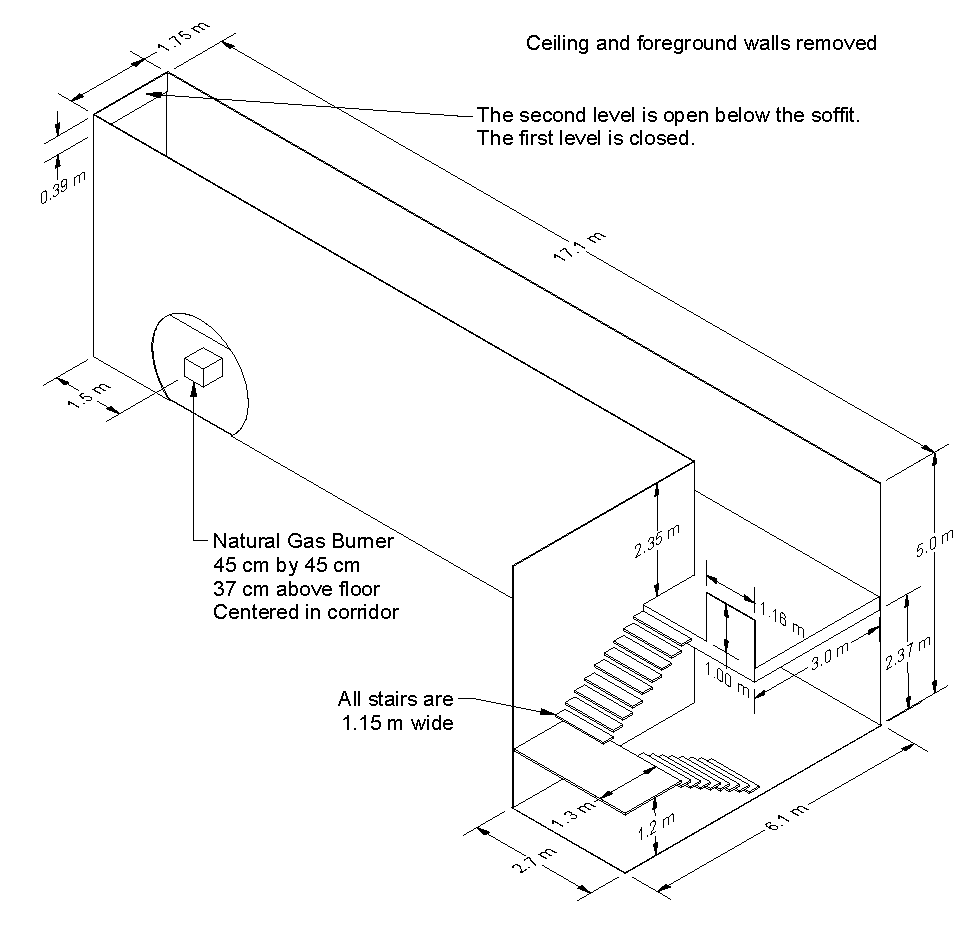
\includegraphics[width=\textwidth]{FIGURES/ATF_Corridors/ATF_Corridors_Drawing}
\caption{Geometry of the ATF Corridors Experiments.}
\label{ATF Drawing}
\end{figure}


\section{Atmospheric Dispersion Correlations}
\label{Atmospheric_Dispersion_Description}

A common exercise in atmospheric dispersion modeling is predicting the plume rise height of stack emissions. Stull~\cite{Stull:2000} presents an empirical correlation for plume rise height from a smoke stack in a stable atmospheric boundary layer. Details of the correlation and simulation are found in Section~\ref{Plume_Height_Discussion}.



\section{Backward Facing Step}
\label{Backward_Facing_Step_Description}

A common validation experiment for CFD codes involves flow through a channel with a backward facing step. These experiments are designed to test the influence of grid resolution, inlet turbulence, wall boundary treatments, and eddy viscosity models. One set of experiments has been conducted by Jovic and Driver~\cite{JD:1994}.  A schematic view of the experiment is shown in Fig.~\ref{tunnel_drawing}. The dimensions of the channel are based on step height $h$ = 0.0098 m.  The length of the channel is $24 \, h$. The width of the channel is $4 \, h$. The height of the inlet section is $5 \, h$, and the height of the channel downstream of the step is $6 \, h$. The expansion ratio is thus 1.2.  The inlet is split into three sub-inlets to permit localized variation of inlet turbulence.  The Reynolds number of the flow is 5100, based on the free-stream velocity (7.2~m/s) and the step height.

\begin{figure}[!ht]
\includegraphics[width=\textwidth]{FIGURES/Backward_Facing_Step/tunnel_drawing}
\caption[Geometry of the Backward Facing Step experiments]{Geometry of the Backward Facing Step experiments.}
\label{tunnel_drawing}
\end{figure}


\section{Beyler Hood Experiments}
\label{Beyler_Hood_Description}

Craig Beyler performed small-scale fire experiments where a variety of circular gas burners were centered at various heights underneath a closed, cylindrical hood, 100~cm in diameter and 48~cm in height~\cite{Beyler:Hood}.  The hood consisted of two concentric cylinders separated by an air gap, as shown in Fig.~\ref{Beyler_Hood_Sketch}.  The inner cylinder was shorter than the outer and this allowed combustion products to be removed uniformly from the hood perimeter.  The exhaust gases were then analyzed to determine species concentrations. The burner could be raised and lowered with respect to the bottom edge of the hood. The reported relative standard uncertainty of the measured gas species mass fractions was 6~\%. The fuels consisted of acetone, ethanol, isopropanol, methanol, propane, propylene, and toluene. Hood equivalence ratios varied from 0.2 to 1.7.  A subset of 47 of the original 148 experiments spanning the equivalence ratio range for each fuel were simulated for validation, see Table~\ref{beyler_sum}.

\begin{figure}[h]
\centering
\includegraphics[width=\textwidth]{FIGURES/Beyler_Hood/Beyler_Hood}
\caption[Sketch of Beyler Hood cross section]{Sketch of Beyler Hood cross section.}
\label{Beyler_Hood_Sketch}
\end{figure}

\begin{table}[!ht]
\centering
\caption[Summary of simulated Beyler Hood experiments]{Summary of simulated Beyler Hood experiments. A negative value of Separation Distance indicates the burner top is below the lower rim of the hood.}
\label{beyler_sum}
\begin{tabular}{|c|c|c|c|c||c|c|c|c|c|}
\hline
Exp.   & Fuel          & HRR      & Burner           & Sep.           &  Exp.   & Fuel          & HRR      & Burner           & Sep.            \\
No.    & Gas           & (kW)     & (cm)             & Dist. (cm)     &  No.    & Gas           & (kW)     & (cm)             & Dist. (cm)      \\ \hline \hline
117    & Acetone       & 18.0     & 22.6             & -12            &  232    & Propane       & 13.5     & 19.5             & -5              \\ \hline
119    & Acetone       & 16.4     & 22.6             & -1             &  257    & Propane       & 8.2      & 19.5             & -15             \\ \hline
122    & Acetone       & 16.4     & 22.6             & 4              &  287    & Propane       & 7.9      & 19.5             & 5               \\ \hline
142    & Acetone       & 12.1     & 22.6             & 4              &  303    & Propane       & 18.3     & 19.5             & 5               \\ \hline
145    & Acetone       & 12.7     & 22.6             & 4              &  307    & Propane       & 21.4     & 19.5             & 5               \\ \hline
106    & Ethanol       & 17.3     & 22.6             & -9             &  318    & Propane       & 18.3     & 19.5             & -20             \\ \hline
107    & Ethanol       & 21.3     & 22.6             & -4             &  322    & Propane       & 21.4     & 19.5             & -20             \\ \hline
108    & Ethanol       & 17.3     & 22.6             & 4              &  334    & Propane       & 21.4     & 19.5             & -15             \\ \hline
110    & Ethanol       & 13.5     & 22.6             & 4              &  355    & Propane       & 18.3     & 19.5             & 0               \\ \hline
115    & Ethanol       & 13.5     & 22.6             & 4              &  359    & Propane       & 21.4     & 19.5             & 0               \\ \hline
130    & Isopropanol   & 12.4     & 22.6             & 4              &  371    & Propane       & 21.4     & 19.5             & -5              \\ \hline
132    & Isopropanol   & 12.4     & 22.6             & 4              &  389    & Propane       & 18.3     & 19.5             & 0               \\ \hline
133    & Isopropanol   & 12.4     & 22.6             & 4              &  429    & Propane       & 28.1     & 19.5             & -10             \\ \hline
136    & Isopropanol   & 12.4     & 22.6             & -1             &  433    & Propane       & 31.5     & 19.5             & -10             \\ \hline
141    & Isopropanol   & 12.4     & 22.6             & 4              &  445    & Propane       & 31.5     & 19.5             & -15             \\ \hline
942    & Methanol      & 11.0     & 22.6             & 0              &  780    & Propylene     & 7.5      & 19.5             & -10             \\ \hline
943    & Methanol      & 11.0     & 22.6             & 0              &  805    & Propylene     & 7.5      & 19.5             & -10             \\ \hline
945    & Methanol      & 11.0     & 22.6             & -5             &  859    & Propylene     & 31.4     & 19.5             & -10             \\ \hline
947    & Methanol      & 11.0     & 22.6             & 0              &  870    & Propylene     & 19.0     & 19.5             & -2              \\ \hline
951    & Methanol      & 9.8      & 22.6             & 0              &  882    & Propylene     & 19.1     & 19.5             & -10             \\ \hline
160    & Toluene       & 11.5     & 22.6             & -6             &  886    & Propylene     & 19.1     & 19.5             & -5              \\ \hline
162    & Toluene       & 11.5     & 22.6             & -1             &  910    & Propylene     & 31.4     & 19.5             & -11             \\ \hline
165    & Toluene       & 11.5     & 22.6             & 4              &  \multicolumn{5}{c|}{}                                                  \\ \cline{1-5}
166    & Toluene       & 11.5     & 22.6             & 5              &  \multicolumn{5}{c|}{}                                                  \\ \cline{1-5}
170    & Toluene       & 11.5     & 22.6             & 4              &  \multicolumn{5}{c|}{}                                                  \\ \hline
\end{tabular}
\end{table}

\subsubsection{Modeling Notes}

Simulations of the Beyler Hood experiments are performed at 3~cm resolution within a fairly simple facsimile of the actual hood. The boundary conditions are set to adiabatic to allow for a relatively quick ramp up to steady-state conditions.

The two-step simple chemistry combustion scheme is applied, where an infinitely fast reaction converts the fuel to CO, soot, and water vapor, followed sequentially by a second fast reaction that converts the soot and CO to CO$_2$. Some of the soot and CO does not convert to CO$_2$, based on post-flame yields listed by Tewarson~\cite{SFPE:Tewarson}.

A minimum auto-ignition temperature is specified for each fuel~\cite{SFPE:Beyler} to prevent the fuel vapor from igniting at the layer interface. This restriction is relaxed in the grid cells just above the burner surface to allow for ignition without a secondary heat source. In addition, a critical flame temperature of 500~$^\circ$C is applied in all cases to account for local flame extinction. The grid is too coarse to support the actual values, and the chosen value is a placeholder until a better flame extinction model is developed.


\section{Bittern Sprinkler Experiments}
\label{Bittern_Sprinkler_Description}

In 2004, a set of 22 fire experiments was conducted at the University of Canterbury, New Zealand, by Adam Bittern~\cite{Bittern:Thesis,Wade:FT2007}. In each experiment, a single chair was burned within an enclosure with two sprinklers installed. The sprinklers were not charged with flowing water during the experiments, but pressure gauges were installed immediately upstream of each sprinkler to indicate activation. The sprinkler actuation time, chair mass loss rate, and gas temperature profile were measured. The HRR was estimated from the measured mass loss rate and heat of combustion of the fuel.

The experiments incorporated four different types of sprinklers, two fire locations (the center and corner of the enclosure), and two ventilation conditions (open or closed door). The enclosure was timber-framed and lined with 10~mm thick gypsum plasterboard. The door was made of plywood and was 0.8~m wide by 2.1~high. The compartment layout, dimensions and experimental arrangement are shown in Figure~\ref{bit_plan}. The chair used as fuel for each experiment was made of flexible polyurethane foam slabs, where each slab measured approximately 0.5~m by 0.4~m by 0.1~m. The seat was ignited using a solid petroleum lighter.

Table~\ref{bit_sum} reports the sprinkler actuation times of each sprinkler.

\begin{figure}[h]
\centering
\includegraphics[width=\textwidth]{FIGURES/Bittern_Sprinkler_Experiments/Bittern_Sketch}
\caption[Plan view of the Bittern Sprinkler Experiments]{Plan view of the Bittern Sprinkler Experiments.}
\label{bit_plan}
\end{figure}


\begin{table}[!ht]
\centering
\caption[Summary of results, Bittern experiments]{Summary of results, Bittern experiments. Note that Exp.~11 has been excluded because of a failed mass loss measurement.}
\label{bit_sum}
\begin{tabular}{|c|c|c|c|c|c|c|c|}
\hline
Exp. & Spr.~1 & Time (s) & Spr.~2 & Time (s) & $T_0$ ($^\circ$C) & Door   & Fire Position \\ \hline \hline
1    & Res A  & 210      & Res A  & 250      & 23.7              & Open   & Center        \\ \hline
2    & Res A  & 225      & Res A  & 211      & 25.5              & Open   & Center        \\ \hline
3    & Res B  & 192      & Res B  & 192      & 25.5              & Open   & Center        \\ \hline
4    & SS68   & 226      & SS68   & 226      & 25.7              & Open   & Center        \\ \hline
5    & SS68   & 266      & SS68   & 272      & 27.5              & Open   & Center        \\ \hline
6    & SS68   & 216      & SS68   & 211      & 27.7              & Open   & Center        \\ \hline
7    & Res A  & 182      & Res A  & 186      & 28.2              & Open   & Center        \\ \hline
8    & Res B  & 182      & Res B  & 187      & 27.9              & Open   & Center        \\ \hline
9    & Res B  & 233      & Res B  & 230      & 28.9              & Open   & Center        \\ \hline
10   & Res A  & 183      & Res B  & 184      & 29.4              & Open   & Center        \\ \hline
12   & SS68   & 246      & Res B  & 228      & 24.0              & Closed & Center        \\ \hline
13   & SS68   & 204      & Res B  & 194      & 24.5              & Closed & Center        \\ \hline
14   & SS68   & 203      & Res B  & 187      & 24.2              & Closed & Center        \\ \hline
15   & SS68   & 270      & Res B  & 253      & 23.7              & Closed & Center        \\ \hline
16   & Res B  & 178      & Res A  & 224      & 20.6              & Closed & Corner        \\ \hline
17   & Res B  & 181      & Res A  & 228      & 23.8              & Closed & Corner        \\ \hline
18   & SS68   & 187      & Res A  & 221      & 25.0              & Closed & Corner        \\ \hline
19   & SS68   & 189      & Res A  & 223      & 26.4              & Closed & Corner        \\ \hline
20   & SS68   & 205      & Res A  & DNA      & 25.3              & Closed & Corner        \\ \hline
21   & SS93   & 216      & SS93   & 330      & 25.2              & Closed & Corner        \\ \hline
22   & SS93   & 205      & SS93   & 263      & 25.2              & Closed & Corner        \\ \hline
\end{tabular}
\end{table}

\subsubsection{Modeling Notes}

The assumptions given in this section were used in the original analysis of the experiments~\cite{Bittern:Thesis}.

The gypsum board had a thickness of 1~cm, density of 731~kg/m\textsuperscript{3}, specific heat of 0.90~kJ/(kg$\cdot$K), conductivity of 0.17~W/(m$\cdot$K), and emissivity of 0.88. The concrete floor was assumed to have a thickness of 10~cm, density of 2300~kg/m$^3$, specific heat of 0.88~kJ/(kg$\cdot$K), conductivity of 1.2~W/(m$\cdot$K), and emissivity of 0.5.

The properties of the sprinklers are shown in Table~\ref{Bittern_Sprinklers}. These properties are based on the manufacturer's specification where available or otherwise estimated based on measured values of comparable sprinklers. For modeling purposes, the sprinkler offset, 2~cm, was selected based on an approximate 2~cm glass bulb length, and the C-factor selected was based on a sensitivity analyses undertaken in the original study.

\begin{table}[!ht]
\centering
\caption[Properties of sprinklers used in Bittern Experiments]{Properties of sprinklers used in Bittern Experiments.}
\label{Bittern_Sprinklers}
\begin{tabular}{|l|l|c|c|c|}
\hline
\textbf{Short} & \textbf{Description}                & \textbf{RTI}        & \textbf{C-Factor} & \textbf{Act. Temp.} \\
\textbf{Name}  &                                     & (m$\cdot$s)$^{1/2}$ & (m/s)$^{1/2}$     & $^\circ$C           \\ \hline
Res A          & Residential, 3 mm glass bulb        & 36                  & 0.4               & 68                  \\ \hline
Res B          & Residential, 3 mm glass bulb        & 36                  & 0.4               & 68                  \\ \hline
SS68           & Standard Response, 5 mm glass bulb  & 95                  & 0.4               & 68                  \\ \hline
SS93           & Standard Response, 5 mm glass bulb  & 95                  & 0.4               & 93                  \\ \hline
\end{tabular}
\end{table}

The average heat of combustion of the upholstery was measured in a cone calorimeter to be 21.9~MJ/kg (Exp.~1-10) and 20.4~MJ/kg (Exp.~12-22). Since the primary fuel used in the experiments was flexible polyurethane foam, the radiant loss fraction assumed in the fire model was 0.46. Other combustion parameters were as for polyurethane foam, and all parameters selected are consistent with those used in the original BRANZFIRE study~\cite{Wade:FT2007}. For the ``simple chemistry'' combustion model, inputs for stoichiometric yields have been selected from literature based on GM23 foam, with an effective molecular formula of CH$_{1.8}$O$_{0.35}$N$_{0.06}$. The soot yield was assumed to be 0.227~kg/kg. The area of the fire was taken to be 0.4~m by 0.5~m. The height of the fire was assumed to be 0.65~m above the floor.

For experiments 11 to 22, the door to the compartment was closed. The estimated leakage area was assumed based on data for loose-fitting internal walls. An area of 0.053 m\textsuperscript{2} was evenly distributed across the door.


\section{Bouchair Solar Chimney}
\label{Bouchair_Solar_Chimney_Description}

To evaluate solar-induced ventilation systems in desert climates, Bouchair~\cite{Bouchair:Thesis} constructed a simple test apparatus shown in Fig.~\ref{Bouchair_Drawing}. A compartment with interior dimensions of approximately 1.6~m long, 1.8~m, and 2.0~m high had a window on one side and an air inlet slot on the other, leading into a 1.5~m wide cavity with two heating panels spanning the long dimension. The panels were heated to 10~$^\circ$C, 20~$^\circ$C, 30~$^\circ$C, or 40~$^\circ$C above ambient, drawing air through the compartment and into the thermal cavity. The mass flow rate of air through the cavity was measured. The inlet slot was either 0.1~m or 0.4~m high, and 1.4~m wide. The thermal cavity was 1.5~m wide, and the hot panels were separated by 0.1~m, 0.2~m, 0.3~m, 0.5~m, or 1.0~m. In all, there were 40 different sets of test parameters.

In addition to the results presented in this guide, simulations of this experiment were performed by Shi and Zhang~\cite{Shi:BE2016}. The objective of the simulations is to predict the mass flow rate by accurately modeling the convective heat transfer between the air and hot panels.

\begin{figure}[!ht]
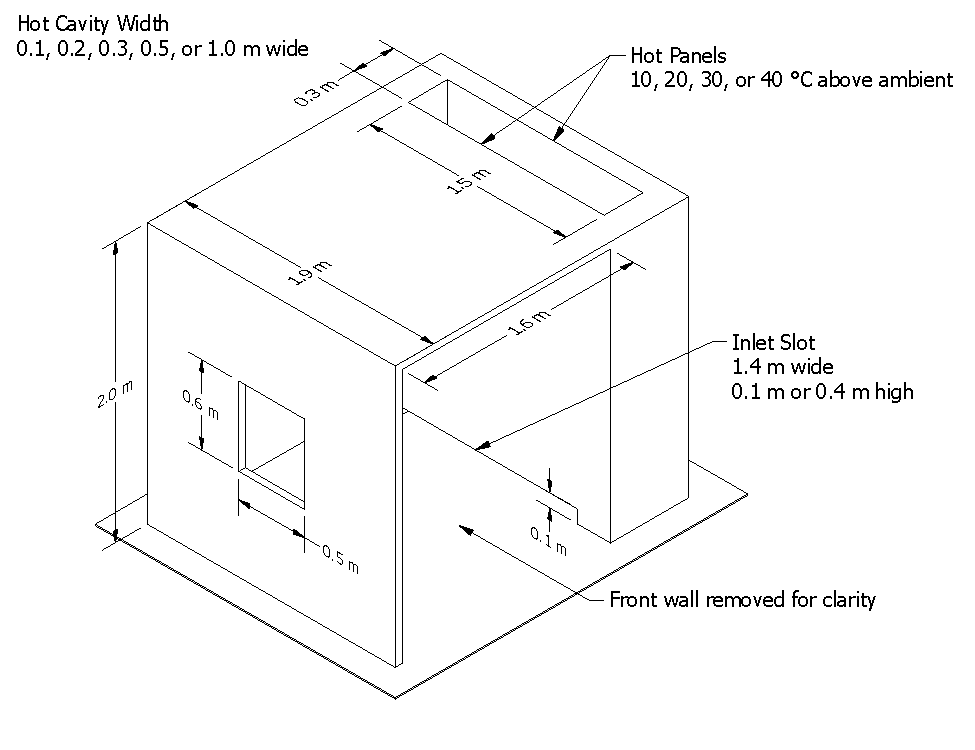
\includegraphics[trim={16in 2.5in 16in 2.5in},clip,width=\textwidth]{FIGURES/Bouchair_Solar_Chimney/Bouchair_Solar_Chimney}
\caption[Geometry of the Bouchair Solar Chimney experiment]{Geometry of the Bouchair Solar Chimney experiment.}
\label{Bouchair_Drawing}
\end{figure}


\section{BRE Spray Test for Radiation Attenuation}
\label{BRE_Spray_Description}

Murrel et al.~\cite{Murrel:1995} measured the attenuation of thermal radiation passing through a water
spray using a heat flux gauge. The radiation was produced by a heat panel, one meter square, at 900~$^\circ$C. The horizontal distance
from the radiation panel to the spray nozzle was 2 m and to the measurement point 4 m. The nozzles were positioned at
a height 0.24 m above the panel upper edge. The heat flux gauge was positioned at the line passing through the center
of the panel. The attenuation of radiation was defined as $(q_0-q_s)/q_0$, where $q_0$ is the initial radiative heat flux,
measured without a spray, and $q_s$ is the heat flux measured during the spray operation.

Experimental results are used from three full-cone type nozzles, labeled A, B and D. The opening angles of the nozzles were between 90 and 108 degrees.
The purpose of the simulation is to compare the measured and simulated attenuation of radiation at different flow conditions. The nozzles were
specified in terms of median droplet size and mean vertical velocity using PDPA measurement in a single position, 0.7 m below the nozzle. The droplet
boundary conditions were determined by assuming $d_m \propto p^{-1/3}$ and $v \propto p^{1/2}$ type of dependencies between the droplet size, speed
and pressure.

\section{Bryant Doorway Velocity Measurements}
\label{Bryant_Doorway_Velocity_Description}

Rodney Bryant of the Fire Research Division at NIST performed a series of velocity measurements of the gas velocity within the doorway of a standard ISO~9705 compartment for fires ranging from 34~kW to 511~kW~\cite{Bryant:FSJ2009,Bryant:EF2009,Bryant:CS2010}. A doorway served as the only vent for the enclosure. It included a jamb of 37~cm extending outward to facilitate the laser measurements. The entire compartment was elevated 0.3~m off the floor of the laboratory (see Fig.~\ref{Bryant_Drawing}). The measurements were made using both bi-directional probes and PIV (Particle Image Velocimetry). The PIV measurements only cover the
lower two-thirds of the doorway because of difficulties in seeding the hot outflow gases. The bi-directional probe measurements span the entire height of the doorway, but Bryant reports that these measurements were up to 20~\% greater than the PIV measurements in certain regions of the flow. Consequently, only the PIV data was used for comparison to the model.

\begin{figure}[ht]
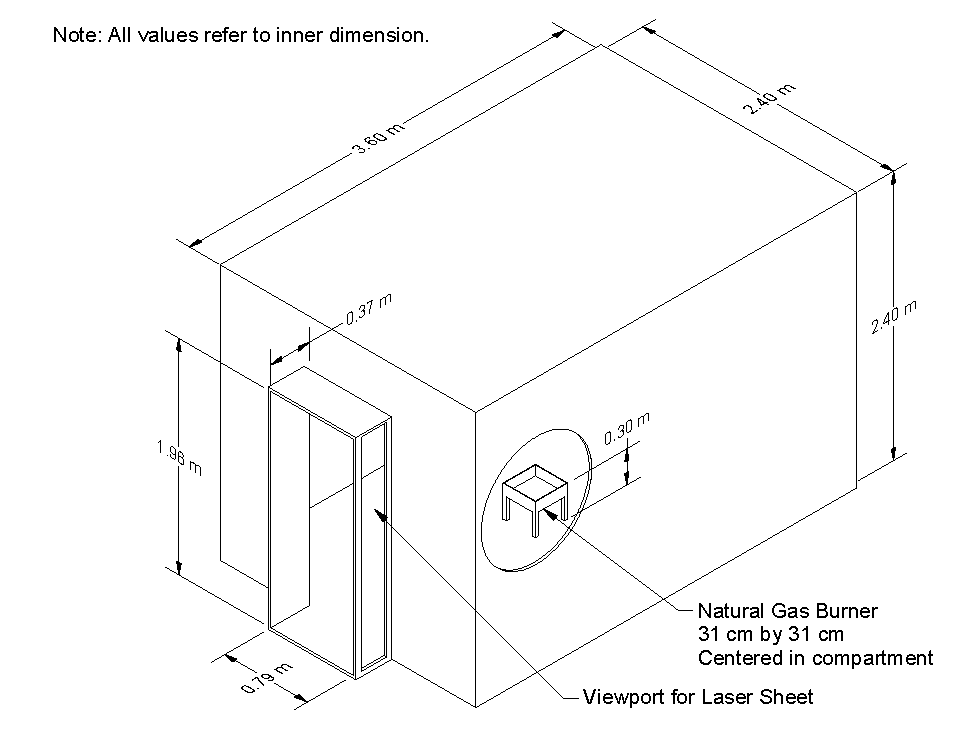
\includegraphics[width=\textwidth]{FIGURES/Bryant_Doorway/Bryant_Compartment}
\caption[Geometry of Bryant's compartment]{Geometry of Bryant's compartment.}
\label{Bryant_Drawing}
\end{figure}


\section{Cable Response to Live Fire -- CAROLFIRE}
\label{CAROLFIRE_Description}

CAROLFIRE was a project sponsored by the U.S.~Nuclear Regulatory Commission to study the thermal response and functional behavior of electrical cables~\cite{CAROLFIRE}. The primary objective of CAROLFIRE was to characterize the various modes of electrical failure (e.g., hot shorts, shorts to ground) within bundles of power, control and instrument cables. A secondary objective of the project was to develop a simple model to predict \underline{th}ermally-\underline{i}nduced \underline{e}lectrical \underline{f}ailure (THIEF). The measurements used for these purposes were conducted at Sandia National Laboratories and are described in Volume II of the CAROLFIRE test report. In brief, there were two series of experiments. The first were conducted within a heated cylindrical enclosure. Single and bundled cables were exposed to various heat fluxes and the electrical failure modes recorded. The second series of experiments involved cables within trays in a semi-enclosed space under which a gas-fueled burner created a hot layer to force cable failure. Only results from the first series are used here.

Petra Andersson and Patrick Van Hees of the Swedish National Testing and Research Institute (SP) proposed that a cable's thermally-induced electrical failure can be predicted via a one-dimensional heat transfer calculation, under the assumption that the cable can be treated as a homogenous cylinder~\cite{Andersson:2005}. Their results for PVC cables were encouraging and suggested that the simplification of the analysis is reasonable and that it should extend to other types of cables. The assumptions underlying the THIEF model are as follows:
\begin{enumerate}
\item The heat penetration into a cable of circular cross section is primarily in the radial direction.
\item The cable is homogeneous in composition. In reality, a cable is constructed of several different types of polymeric materials, cellulosic fillers, and a conducting metal, most often copper.
\item The thermal conductivity, specific heat, and density of the assumed homogeneous cable are independent of temperature. In reality, both the thermal conductivity and specific heat of polymers are temperature-dependent, but this information is not easily obtained from manufacturers.
\item It is assumed that no decomposition reactions occur within the cable during its heating, and ignition and burning are not considered in the model. In fact, thermoplastic cables melt, thermosets form a char layer, and both release volatile gases up to and beyond the point of electrical failure.
\item Electrical failure occurs when the temperature just inside the cable jacket reaches an experimentally determined value.
\end{enumerate}



\section{Crown Fires}
\label{Crown_Fires_Description}

The term ``crown fire'' refers to a wildfire that spreads from the ground surface into the tree canopy. Alexander and Cruz~\cite{Alexander:CJFR2006} compiled a data set of 57 crown fires that occurred in the U.S. and Canada between 1965 and 2003. For each fire, the relative humidity, ambient temperature, and dominant vegetation type are reported, along with estimated values for the vegetation moisture content, {\em canopy}\footnote{Note the difference between {\em canopy} bulk density and {\em crown} bulk density, both of which are abbreviated CBD. The former is the bulk density over the entire forested area, whereas the latter refers to the bulk density within the crown of an individual tree.} bulk density, and open 10~m wind speed. The vegetation consists mainly of coniferous trees, like pines and spruces, and dry undergrowth and ground cover, i.e. scrub brush and dry pine needles. The reported relative humidity ranges between 5~\% and 50~\%, the estimated moisture content ranges between 5~\% and 10~\%, the estimated {\em canopy} bulk density ranges between 0.1~kg/m$^3$ and 0.2~kg/m$^3$, the estimated wind speed ranges between 10~km/h and 50~km/h, and the observed rate of spread ranges between 10~m/min and 110~m/min.

\subsubsection{Modeling Notes}

It is not possible to compare directly the model simulations with the observed fires because of lack of information about the number, spacing, and height of the trees; and the depth, mass, and composition of the ground cover. Instead, Ziegler~et~al.~\cite{Ziegler:thesis,Ziegler:FEM2017,Ziegler:Data2019,Hoffman:FT2016} developed tree maps based on various forests found in the western region of the U.S. The maps contain the location and rough dimensions of each tree in a 4~ha area. Eight maps were developed based on four specific locations and pre- or post-treated conditions. In addition, Ziegler~et~al.~suggest that the moisture content of the trees is approximately 100~\%, and the ground cover 5~\%. The {\em crown} bulk density for all simulations is 1.2~kg/m$^3$, and the surface density is 0.72~kg/m$^2$ with a depth of 6~cm. The simulated fires are ignited along a strip, and the rate of spread is calculated based on the position of peak temperature.

The simulations are performed with a numerical grid that has a resolution of 1~m by 1~m by 0.5~m near the ground, and the vertical dimension increases gradually with height. Because of this relatively coarse resolution, the burning rate of the vegetation is limited to ensure that any given patch of surface vegetation or volume of canopy vegetation cannot burn completely in less than 30~s.





\section{CSIRO Grassland Fires}
\label{CSIRO_Grassland_Fires_Description}

In July and August of 1986, the Commonwealth Scientific and Industrial Research Organisation (CSIRO) of Australia conducted controlled grassland fire experiments near Darwin, Northern Territory~\cite{Cheney:IJWF1993}. July and August are in the middle of the dry season when the grasses are fully cured (dried) and the weather is warm and dry. The experiments were conducted on flat plots measuring 100~m by 100~m, 200~m by 200~m, or 200~m by 300~m. Two cases have been simulated. Case~C064 was conducted on a 100~m by 100~m plot of kerosene grass ({\it Eriachne burkittii}); Case~F19 was conducted on a 200~m by 200~m plot of kangaroo grass ({\it Themeda australis}).

\subsubsection{Modeling Notes}

Two of these experiments were originally simulated with FDS by Mell~et~al.~\cite{Mell:IJWF2007}. These simulations modeled the grass as a collection of cylindrical Lagrangian particles. The pyrolysis model assigned to the particles is described in the FDS User's Guide~\cite{FDS_Users_Guide}, chapter ``Earth, Wind and Fire,'' Section~\ref{UG-vegetation_model}, ``Thermal Degradation Model for Vegetation.''

Now these two experiments are also simulated using the Boundary Fuel Model (BFM)~\cite{Perez-Ramirez:FT2017} and the Rothermel-Albini fire spread algorithm~\cite{Rothermel:1972,Albini:1976}. For the experiment labelled Case~C064, fuel index 1 (Short Grass) is used, with a modified moisture fraction of 0.063. For F19, fuel index 3 (Tall Grass) is used, with a modified moisture fraction of 0.058.

Measured properties for the specific types of grasses burned in the two experiments are listed in Table~\ref{Properties_Grasses}. Properties that were not measured are listed in Table~\ref{Assumed_Properties_Grasses}. These assumed properties are typically for wood or cellulosic fuels. The moisture is modeled as water. The grass is assumed to be composed primarily of cellulose.



\begin{figure}[ht]
\includegraphics[width=\textwidth]{FIGURES/CSIRO_Grassland_Fires/Case_F19_0358.png}
\caption[Snapshot of the simulation of CSIRO Grassland Fire F19]{Snapshot of the simulation of CSIRO Grassland Fire F19.}
\label{F19}
\end{figure}

A snapshot of the Lagrangian particle simulation of Case~F19 is shown in Fig.~\ref{F19}. The computational domain in this case is 240~m by 240~m by 20~m. The grid cells are 0.5~m cubes. The domain is subdivided into 36 individual meshes and run in parallel. The grass is represented 1 simulated blade per grid cell. The radius of the cylinder is derived from the measured surface area to volume ratio. Each simulated blade of grass represents many more actual blades of grass. The weighting factor is determined from the measured bulk mass per unit area. The fires in the experiments were ignited by two men carrying drip torches walking in opposite directions along the upwind boundary of the plot (the red strip in Fig.~\ref{F19}). In FDS, this action was modeled using a specified spread rate along the strip.

\begin{table}[ht]
\begin{center}
\caption[Measured properties for the CSIRO Grassland Fire cases]{Measured properties for the CSIRO Grassland Fire cases~\cite{Cheney:IJWF1993}.}
\label{Properties_Grasses}
\begin{tabular}{|l|c|c|c|}
\hline
Property                        & Units         & Case F19      & Case C064     \\ \hline \hline
Wind Speed                      & m/s           & 4.8           & 4.6           \\ \hline
Ambient Temperature             & $^\circ$C     & 34            & 32            \\ \hline
Surface Area to Volume Ratio    & m$^{-1}$      & 12240         & 9770          \\ \hline
Grass Height                    & m             & 0.51          & 0.21          \\ \hline
Bulk Mass per Unit Area         & kg/m$^2$      & 0.313         & 0.283         \\ \hline
Moisture Fraction               & \%            & 5.8           & 6.3           \\ \hline
\end{tabular}
\end{center}
\end{table}

\begin{table}
\begin{center}
\caption[Assumed properties for dry grass and soil]{Assumed properties for various types of dried grass and soil. Note that the Pyrolysis Temperature is taken to be the temperature at which the mass loss rate peaks in the TGA experiments of Morvan and Dupuy~\cite{Morvan:CF2004}.}
\label{Assumed_Properties_Grasses}
\begin{tabular}{|l|c|c|c|}
\hline
Property                        & Units                 & Value                     & Reference                             \\ \hline \hline
Chemical Composition            & --                    & C$_6$H$_{10}$O$_5$        & Assumption                            \\ \hline
Heat of Combustion              & kJ/kg                 & 15600                     & \cite{Susott:FS1982}                  \\ \hline
Soot Yield                      & kg/kg                 & 0.015                     & \cite{SFPE:Tewarson}                  \\ \hline
Char Yield                      & kg/kg                 & 0.2                       & \cite{Susott:FS1982}                  \\ \hline
Specific Heat                   & kJ/(kg$\cdot$K)       & 1.5                       & Various sources                       \\ \hline
Conductivity                    & W/(m$\cdot$K)         & 0.1                       & Assumption                            \\ \hline
Density                         & kg/m$^3$              & 512                       & \cite{Rothermel:1972}                 \\ \hline
Heat of Pyrolysis               & kJ/kg                 & 418                       & \cite{Morvan:CF2004}                  \\ \hline
Pyrolyis Temperature            & $^\circ$C             & 200                       & \cite{Morvan:CF2004}                  \\ \hline \hline
Obukhov Length                  & m                     & -500                      & Assumption                            \\ \hline
Aerodynamic Roughness Length    & m                     & 0.03                      & Assumption                            \\ \hline
Drag Coefficient                & --                    & 2.8                       & \cite{Falkenstein-Smith:2018}         \\ \hline \hline
Soil Specific Heat              & kJ/(kg$\cdot$K)       & 2.0                       & \cite{Farouki:1981}                   \\ \hline
Soil Conductivity               & W/(m$\cdot$K)         & 0.25                      & \cite{Farouki:1981}                   \\ \hline
Soil Density                    & kg/m$^3$              & 1300                      & \cite{Farouki:1981}                   \\ \hline

\end{tabular}
\end{center}
\end{table}


\section{CSTB Tunnel Experiments}

Between 2005 and 2008, the French building research laboratory, Centre Scientifique et Technique du B\^{a}timent (CSTB) cooperated with the French Tunnel Study Center (CETU), the French National Centre for Scientific Research (CNRS, Institut PPRIME) and the French Directorate for Civil Security (DSC) to conduct fire experiments in a tunnel, some of which involved a water mist system~\cite{Meyrand,Blanchard:FT2014}. The first aim was to improve the understanding of the interaction between water mist and a tunnel fire.  The second was to develop a database for model validation. A one-third scale was selected with the objective of studying realistic fire phenomena in an affordable way.  Twenty-eight experiments were conducted (20 with and 8 without water mist) with varying fuels (heptane pool, wood crib, and wood pallet) and longitudinal velocities (with and without back layering).

The tunnel was 43~m long, with a semi-circular cross section whose area was approximately 4~m$^2$. The walls were covered by a fire resistant mortar cement with well known thermal properties. The floor was made of concrete. A fan was mounted at the downstream side of the tunnel.  Measurements were made of the following: fuel mass, gas temperature, air velocity, radiative heat flux and gas concentration (CO, CO$_2$ and O$_2$).  Sensors were located at 11 longitudinal positions.

Tests~2 and 27 have been selected because neither exhibited back layering. The longitudinal velocity in Test~2 was approximately 2.2~m/s and in Test 27 it was 3.1~m/s. Both experiments involved a 0.5~m$^2$ area heptane pool. In Test~2, the HRR was deduced from the fuel mass loss rate only.  In Test~27, the HRR was deduced from both the mass loss rate and from oxygen consumption calorimetry.

In Test 27, a water mist system was manually activated 300~s after ignition. The water mist system was composed of six nozzles along the centerline of the tunnel, from 4~m upstream to 3.5~m downstream of the fire, 1.5~m apart.  The operating pressure was approximately 90~bar. The water flow rate injected at each nozzle was close to 5.5~L/min, corresponding to a total mist discharge rate of approximately 33~L/min.  Test~27 is interesting because it involved a very low water injection rate.  The main consequence is that the HRR actually increased slightly after the nozzles were activated, and the fire did not extinguish.  The experiment stopped when the fuel was exhausted. This allowed for an assessment of the model's ability to predict the gas cooling and radiation attenuation.

\subsubsection{Modeling Notes}

The simulations of these experiments are performed using 12 meshes. To prevent numerical instability due to oscillations in pressure, a common problem for tunnel fire simulations, the {\ct VELOCITY\_TOLERANCE} and {\ct PRESSURE\_TOLERANCE} are reduced to 0.01~m/s and 400~s$^{-2}$, respectively, and the {\ct MAX\_PRESSURE\_ITERATIONS} is increased to 50. The multi-port mist nozzles are each modeled as a collection of single nozzles with varying orientations.



\section{Cup Burner Experiments}
\label{Cup_Burner_Description}

The cup-burner is a widely used experimental apparatus for studying the effectiveness of flame extinguishing agents. Typically, these experiments feature a steady fuel-air co-flow diffusion flame that is established above the cup. The extinguishing agent is gradually introduced into the air stream to determine the minimum concentration of the agent that leads to lift off. One hundred and ten experimental data sets are examined. The data sets include sixteen fuels: acetone, acetylene, benzene, butane, dodecane, ethanol, ethylene, heptane, hexane, hydrogen, methane, methanol, octane, propanol, and toluene, and five inert gases: argon (Ar), carbon dioxide (CO$_2$), helium (He), and nitrogen (N$_2$), and sulfur hexaflouride (SF$_6$). A STANJAN\footnote{STANJAN is a program for chemical equilibrium calculations.} calculation has been performed to determine the equilibrium temperature using the measured minimum extinguishing concentration for each experiment. The calculation assumes constant pressure and enthalpy using a stoichiometric mixture of fuel and air plus agent. For combinations of fuel and agent with multiple experiments, the average extinguishing concentration and the average flame temperature is taken, resulting in forty-six unique combinations of fuel and agent listed in Table~\ref{Cup_Table}.

\begin{table}[p]
\caption{Summary of Cup Burner Data}
\label{Cup_Table}
\small
\begin{tabular}{|l|c|c|c|c|l|}
\hline
Fuel       &  Agent  & MEC  & CFT  & References   \\ \hline \hline
Acetone    & Ar      & 34.0 & 1729 & \cite{Tapscott:1,Moore:1}  \\ \hline
Acetone    & CO$_2$  & 19.0 & 1678 & \cite{Yamamoto:1}  \\ \hline
Acetone    & N$_2$   & 28.0 & 1670 & \cite{Tapscott:1,Yamamoto:1}  \\ \hline
Acetylene  & CO$_2$  & 45.0 & 1338 & \cite{Yamamoto:1}  \\ \hline
Acetylene  & N$_2$   & 58.0 & 1312 & \cite{Yamamoto:1}  \\ \hline
Benzene    & CO$_2$  & 20.1 & 1691 & \cite{Yamamoto:1,Sakei:1}  \\ \hline
Benzene    & N$_2$   & 30.3 & 1683 & \cite{Tapscott:1,Yamamoto:1,Sakei:1}  \\ \hline
Butane     & N$_2$   & 31.0 & 1594 & \cite{Yamamoto:1}  \\ \hline
Butane     & CO$_2$  & 19.0 & 1639 & \cite{Yamamoto:1}  \\ \hline
Dodecane   & N$_2$   & 33.0 & 1577 & \cite{Tapscott:1}  \\ \hline
Ethanol    & Ar      & 36.5 & 1654 & \cite{Tapscott:1,Moore:1}  \\ \hline
Ethanol    & CO$_2$  & 23.7 & 1542 & \cite{Yamamoto:1,Sakei:1}  \\ \hline
Ethanol    & N$_2$   & 34.6 & 1529 & \cite{Tapscott:1,Yamamoto:1,Sakei:1}  \\ \hline
Ethylene   & CO$_2$  & 32.0 & 1471 & \cite{Yamamoto:1}  \\ \hline
Ethylene   & N$_2$   & 45.0 & 1441 & \cite{Yamamoto:1}  \\ \hline
Heptane    & Ar      & 39.5 & 1643 & \cite{Tapscott:1,Bogdan:1,Moore:1,Sheinson:FSJ,Grosshandler:Cup,Saito:FSJ,NFPA_2001,ISO_14520,Senecal:FSJ}  \\ \hline
Heptane    & N$_2$   & 31.2 & 1617 & \cite{Tapscott:1,Bogdan:1,Hamins:CS1998,Moore:1,Hirst:1,Sheinson:FSJ,Grosshandler:Cup,Saito:FSJ,Yamamoto:1,Sakei:1,NFPA_2001,ISO_14520,Senecal:FSJ}  \\ \hline
Heptane    & CO$_2$  & 21.4 & 1617 & \cite{Moore:1,Hirst:1,Sheinson:FSJ,Grosshandler:Cup,Saito:FSJ,Yamamoto:1,Sakei:1}  \\ \hline
Heptane    & He      & 31.5 & 1763 & \cite{Sheinson:FSJ,Grosshandler:Cup}  \\ \hline
Heptane    & SF$_6$  & 11.0 & 1531 & \cite{Sheinson:FSJ}  \\ \hline
Hexane     & Ar      & 33.0 & 1740 & \cite{Moore:1}  \\ \hline
Hexane     & CO$_2$  & 20.0 & 1647 & \cite{Yamamoto:1}  \\ \hline
Hexane     & N$_2$   & 29.0 & 1646 & \cite{Tapscott:1,Yamamoto:1}  \\ \hline
Hydrogen   & CO$_2$  & 60.0 &  913 & \cite{Yamamoto:1}  \\ \hline
Hydrogen   & N$_2$   & 72.0 &  870 & \cite{Yamamoto:1}  \\ \hline
Methane    & Ar      & 33.8 & 1659 & \cite{Tapscott:1,Takahashi:CS2007,Moore:1}  \\ \hline
Methane    & N$_2$   & 24.2 & 1663 & \cite{Takahashi:CS2007,Yamamoto:1,Ural:1}  \\ \hline
Methane    & CO$_2$  & 14.4 & 1694 & \cite{Yamamoto:1,Sakei:1}  \\ \hline
Methane    & He      & 26.7 & 1746 & \cite{Takahashi:CS2007}  \\ \hline
Methanol   & Ar      & 45.0 & 1494 & \cite{Tapscott:1,Moore:1}  \\ \hline
Methanol   & CO$_2$  & 29.2 & 1410 & \cite{Yamamoto:1,Sakei:1}  \\ \hline
Methanol   & N$_2$   & 40.8 & 1395 & \cite{Tapscott:1,Yamamoto:1,Sakei:1}  \\ \hline
Octane     & Ar      & 27.0 & 1790 & \cite{Moore:1}  \\ \hline
Octane     & CO$_2$  & 24.0 & 1542 & \cite{Yamamoto:1}  \\ \hline
Octane     & N$_2$   & 33.0 & 1564 & \cite{Tapscott:1,Yamamoto:1}  \\ \hline
Propane    & Ar      & 37.5 & 1652 & \cite{Tapscott:1,Moore:1}  \\ \hline
Propane    & CO$_2$  & 21.0 & 1600 & \cite{Yamamoto:1}  \\ \hline
Propane    & N$_2$   & 32.3 & 1573 & \cite{Hamins:CS1998,Yamamoto:1,Ural:1}  \\ \hline
Propanol   & Ar      & 28.0 & 1781 & \cite{Moore:1}  \\ \hline
Propanol   & CO$_2$  & 22.0 & 1584 & \cite{Yamamoto:1}  \\ \hline
Propanol   & He      & 30.0 & 1755 & \cite{Sheinson:FSJ}  \\ \hline
Propanol   & N$_2$   & 30.0 & 1608 & \cite{Yamamoto:1,Sheinson:FSJ}  \\ \hline
Propanol   & SF$_6$  & 11.0 & 1515 & \cite{Sheinson:FSJ}  \\ \hline
Toluene    & Ar      & 27.0 & 1854 & \cite{Moore:1}  \\ \hline
Toluene    & CO$_2$  & 17.0 & 1744 & \cite{Yamamoto:1,Sakei:1}  \\ \hline
Toluene    & N$_2$   & 24.4 & 1755 & \cite{Yamamoto:1,Sakei:1}  \\ \hline
\end{tabular}
\noindent
\begin{tabbing}
MEC  \hspace{0.05in} \= Minimum Extinguishing Concentration (mol/mol) \\
CFT                  \> Critical Flame Temperature ($^\circ$C)
\end{tabbing}
\end{table}


\subsubsection{Modeling Notes}

Cup burner dimensions, fuel inlet velocity, and co-flow inlet velocity vary slightly amongst the researchers; however, extinguishing concentrations have been shown to be fairly insensitive over the range of typical values. The cup burner model was implemented as a 2D, cylindrical geometry with a 1 cm radius for the burner and a 4 cm radius for the tube. A 1 mm grid resolution was used. For gaseous fuels a 1 cm/s inlet velocity was used for the burner. Liquid fuels used burning rates from the SFPE Handbook; fuels without published burning rates scaled the burning rate of a chemically similar fuel (e.g. alcohol, alkane) using the heat of vaporization for the fuel. The fuel temperature boundary condition was ambient for gaseous fuels and one-half of the boiling point for liquid fuels. The co-flow was set to 12~cm/s. The agent mass fraction was ramped from approximately 10~\% below to 10~\% above the values shown in Table~\ref{Cup_Table}. The {\ct CRITICAL\_FLAME\_TEMPERATURE} was set to the values in Table~\ref{Cup_Table}.

\section{DelCo Trainer Experiments}
\label{DelCo_Description}

The NIST Fire Fighting Technology Group conducted a series of experiments in two structures of similar design located at the Delaware County (``DelCo'') Emergency Services Training Center in Sharon Hill, Pennsylvania~\cite{DelCo_TN}. Three propane burners were used to provide the fire source for all experiments, and various sensors were used to collect gas temperature, gas velocity, heat flux, and gas concentration measurements throughout the structure.

The single level structure was instrumented with five bare-bead thermocouple arrays and two gas sample inlet pipes at the locations shown in Fig.~\ref{fig:east_instrumentation}. Both floors of the two level structure were instrumented with three bare-bead thermocouple arrays and one gas sample inlet pipe at the locations shown in Fig.~\ref{fig:west_instrumentation}.

\begin{figure}[!ht]
\includegraphics[width=\columnwidth]{FIGURES/DelCo_Trainers/East_Structure_Dimensioned_Instrumentation}
\caption[Instrumentation of the single level DelCo training structure]{Instrumentation of the single level DelCo training structure. The thermocouple arrays are denoted by crossed circles and the gas sampling measurement locations are denoted by hexagons at locations A1 and A4. The burner is denoted by three cross-hatched squares.}
\label{fig:east_instrumentation}
\end{figure}

\begin{figure}[p]
\includegraphics[width=0.94\columnwidth]{FIGURES/DelCo_Trainers/West_Structure_2nd_Floor_Dimensioned_Instrumentation}
\\~\\
\includegraphics[width=\columnwidth]{FIGURES/DelCo_Trainers/West_Structure_1st_Floor_Dimensioned_Instrumentation}
\caption[Instrumentation of the two level DelCo training structure]{Instrumentation of the second floor (top) and first floor (bottom) of the two level DelCo training structure. The thermocouple arrays are denoted by crossed circles and the gas sampling measurement locations are denoted by hexagons at locations A1 and A10. The burner is denoted by three cross-hatched squares.}
\label{fig:west_instrumentation}
\end{figure}

\section{Droplet Evaporation}
\label{Droplet_Evaporation_Description}

Five sets of experiments have been selected for validation of the evaporation of liquid droplets.

\subsubsection{Fujita, Kurose, and Komori Experiments}
\label{Fujita_exp}

Fujita, Kurose, and Komori performed a series of experiments that suspended a water drop in a heated, vertical wind tunnel~\cite{Fujita}. Four experiments were modeled with relative humidity values of 0~\% and 30~\% and droplet Reynolds numbers of 60 and 150 (approximately 0.8~m/s and 2.0~m/s). Droplet size and surface temperature were recorded as functions of time.

\subsubsection{Gavin Experiments}
\label{Gavin_exp}

Gavin performed two experiments of a single water drop falling in dry air~\cite{Gavin}. The test apparatus was a vertical wind tunnel. A drop was injected into the wind tunnel and the vertical air stream velocity was changed over time to maintain the drop at a constant elevation in the wind tunnel. The first droplet was 769~$\mu$m with an initial temperature of 23.0~$^\circ$C. The second droplet was 557~$\mu$m with an initial temperature of 24.3~$^\circ$C.

\subsubsection{Kolaitis and Founti Experiments}
\label{Kolaitis_exp}

Kolaitis and Founti measured the diameter and temperature of suspended liquid fuel droplets in a heated air stream~\cite{Kolaitis}. Four experiments were chosen: a 1.26~mm droplet of ethanol at an initial temperature of 34.2~$^\circ$C in 94~$^\circ$C quiescent air, a 1.13~mm droplet of decane at an initial temperature of 73.8~$^\circ$C in 94~$^\circ$C quiescent air, a 1.15~mm droplet of heptane at an initial temperature of 49.0~$^\circ$C in 94~$^\circ$C quiescent air, and a 1.42~mm droplet of heptane at an initial temperature of 15.5~$^\circ$C in 94~$^\circ$C air at 0.146~m/s.

\subsubsection{Maqua, Castanet, and Lemoine Experiments}
\label{Maqua_exp}

Maqua, Castanet, and Lemoine measured the temperature of falling droplets of ethanol and acetone mixtures in a heated plume~\cite{Maqua}. Because the temperature and velocity of the plume was not well-characterized, only the experiments involving a droplet falling in quiescent air were modeled. As FDS does not currently have a sub-model for the evaporation of a multi-component fuel, only the experiments for a pure ethanol droplet (140~$\mu$m) and a pure acetone droplet (140~$\mu$m) were modeled. The initial droplet temperature in both experiments was 45~$^\circ$C in 20~$^\circ$C air.

\subsubsection{Taflin Experiments}
\label{Taflin_exp}

Taflin measured the diameter of suspended water droplets in dry air~\cite{Snegirev:1}. One droplet was initially 43.9~$\mu$m and the other was 56.6~$\mu$m.

\section{FAA Cargo Compartments}
\label{FAA_Cargo_Description}

The U.S.~Federal Aviation Administration (FAA) has sponsored experiments and modeling of smoke transport within aircraft storage compartments~\cite{FAA-AR-03-49,FAA-AR-07-27}. Two types of compartments were used; one from a Boeing~707 and one from a McDonnell Douglas DC-10. The 707 compartment was 6.7~m in length, 3.2~m in width, and 1.4~m in height. The DC-10 compartment was 14~m in length, 4.4~m in width, and 1.7~m in height. The fire for all experiments was fueled by a 0.1~m by 0.1~m tray of plastic resin producing a peak HRR of 5~kW~\cite{FAA-AR-06-21}. The long walls of the compartments were barrel-shaped to conform to the shape of the aircraft fuselage. The fire was placed in different locations, and measurements of gas and ceiling temperature, heat flux, gas concentration, and smoke obscuration were made at a variety of locations, mostly near the ceiling.


\section{FAA Polymers}
\label{FAA_Polymers_Description}

As part of their efforts to characterize the burning behavior of commonly used plastics, the U.S.~Federal Aviation Administration (FAA) conducted measurements of the thermal properties of charring and non-charring polymers with the specific purpose of providing input data for numerical pyrolysis models~\cite{Stoliarov:CF2009,Stoliarov:CF2010}. The study aimed to determine whether a one-dimensional conduction/reaction model could be used as a practical tool for prediction and/or extrapolation of the results of fire calorimetry tests. The non-charring polymers included poly(methyl methacrylate) (PMMA), high-impact polystyrene (HIPS), and high density polyethylene (HDPE). The charring polymers included polycarbonate (PC) and polyvinyl chloride (PVC).


\section{Fleury Heat Flux Measurements}
\label{Fleury_Heat_Flux_Description}

Rob Fleury, a master's degree student at the University of Canterbury in Christchurch, New Zealand, measured the heat flux from a variety of propane fires~\cite{Fleury:Masters}. The objective of the work was to evaluate a variety of empirical heat flux calculation methods. For the measurements, heat flux gauges were mounted on moveable dollies that were placed in front of, and to the side of, burners with dimensions of 0.3~m by 0.3~m (1:1 burner), 0.6~m by 0.3~m (2:1 burner), and 0.9~m by 0.3~m (3:1 burner). The heat release rates were set to 100~kW, 150~kW, 200~kW, 250~kW, and 300~kW. The gauges were mounted at heights of 0~m, 0.5~m, 1.0~m, and 1.5~m relative to the top edge of the burner.


\section{FM Burner Experiments}
\label{FM_Burner_Description}

A series of gas burner experiments was conducted by Zeng and Wang at FM Global in which the co-flow air stream was gradually diluted with nitrogen until flame extinction was achieved~\cite{Zeng:26ICDERS}. Numerical simulations were subsequently performed by Ren~et~al.~\cite{Ren:CS2018}. In the experiments, a cylindrical, water-cooled steel burner (15.2~cm O.D., 13.7~cm I.D.) was placed near the floor of a 1.22~m by 1.22~m by 1.83~m tall compartment. Four fuels were used: ethylene (C$_2$H$_4$), methane (CH$_4$), propane (C$_3$H$_8$), and propylene (C$_3$H$_6$). The heat release rate in each experiment was 10~kW with a 1~kW ring of pilot burners to stabilize the flame. At the start of each experiment, air was pumped through the floor at a rate sufficient to supply the fire with approximately 10 times the stoichiometric requirement. Subsequently, nitrogen was slowly added to the air stream until the fire was extinguished.

In the same enclosure and using the same burner, Ren et. al~\cite{Ren:IAFSS2020} made high-frequency mean and rms temperature measurements along six radial profiles above a 15~kW ethylene fire. Soot measurements were made at similar locations. The co-flow air stream at the floor was set to 20.9~\%, 16.8~\%, and 15.2~\% oxygen volume fraction. Additional experiments were performed at 19~\%, 17~\%, and 15~\% oxygen in which global radiation measurements were made, including total radiative fraction and the vertical distribution of radiative emission.

\subsubsection{Modeling Notes}

The FDS simulations of the 10~kW ethylene, methane, propane and propylene fires are run for 65~s, in which time the oxygen concentration in the co-flow stream is ramped down linearly from 21~\% to 8~\%. The volume flow of the co-flow stream has been increased tenfold compared to the experiments to prevent a downwash of ambient air into the sealed compartment. The 15~kW ethylene fire simulations at the various fixed oxygen levels are performed for 20~s. For these simulations, the oxygen volume fraction is specified directly, as is the co-flow stream.

The combustion and extinction are modeled using a two-step reaction scheme. In the first step, fuel is converted to CO, soot, and water vapor, and in the second step, the CO and soot are oxidized to form CO$_2$. Both reactions are fast, but the oxidation step follows the first reaction in serial. That is, in a given time step, all available oxygen first converts fuel to CO and Soot, assumed to be C$_{0.9}$H$_{0.1}$. Any leftover oxygen is then used to oxidize existing CO and Soot. There are two assumptions. First, it is assumed that 2/3 of the carbon in the fuel molecule is converted to CO, and 1/3 to Soot in the first reaction step. Second, the post-flame yields of Soot and CO are set to 0.043 and 0.013, respectively, based on Tewarson's measurements reported in the SFPE Handbook~\cite{SFPE:Tewarson}.

Under the assumption that Air contains 383~ppm CO$_2$ and water vapor corresponding to 40~\% humidity, the full two-step reaction scheme for ethylene is written in terms of ``lumped'' species as follows:
\begin{eqnarray}
\lefteqn{ \underbrace{\mathrm{ (C_2H_4) }}_\text{Fuel} \; + \;
7.96 \; \underbrace{ \mathrm{\left( 0.208 \, O_2 + 0.783 \; N_2 + 0.0004 \, CO_2 + 0.009 \, H_2O \right)}}_\text{Air} \longrightarrow } \quad \quad \quad \quad \quad \quad \quad \nonumber \\
& & 10.34 \, \underbrace{\mathrm{(0.130 \; CO +  0.197 \; H_2O + 0.071 \; Soot +  0.602\, N_2 + 0.0003 \, CO_2)}}_\text{Products 1}
\end{eqnarray}
\be
(\text{Products 1}) + 0.58 \; (\text{Air}) \longrightarrow  1.45 \, \underbrace{\mathrm{(0.0009 \, CO + 0.0073 \, Soot + 0.126 \, CO_2 +  0.141 \; H_2O  + 0.725 \; N_2)}}_\text{Products 2}
\ee
For each of the four fuels simulated, it has been assumed that 2/3 of the carbon in the fuel molecule is converted to CO in the first step. However, there are only detailed measurements of radiative emission and soot volume fraction for ethylene. Thus, it is not clear how the carbon is distributed between the soot and CO in the early stages. For lighter sooting fuels like methane, the fraction of carbon allocated to CO approaches unity.

The radiative fraction has been predicted rather than specified in all simulations.



\section{FM/FPRF Data Center Experiments}
\label{FM_FPRF_Datacenter_Description}

The Fire Protection Research Foundation funded a series of large scale tests of smoke detection in high airflow data centers as part of a research project on behalf of the NFPA~75 and NFPA~76 Technical Committees~\cite{FM_Datacenter_Rpt}. The tests consisted of a data center mockup that was 4.9~m high, 4.9~m wide, and 7.3~m deep. The mockup was divided into a 0.9~m tall subfloor with air supplied via a natural vent opening on one short wall, a 0.9~m tall ceiling plenum with air removed via a mechanical vent opening on one short wall, two 2~m tall by 0.6~m wide by 5.3~m long enclosed cold aisles located along the outer walls, and a 3.1~m tall hot aisle.  Flow from the subfloor to the cold aisles occurred through grated floor tiles, flow from the cold aisles to the hot aisle was through two rows of empty equipment cabinets with perforated metal doors, and flow from the hot aisle to the ceiling plenum was through perforated metal ceiling tiles.

Two groups of tests were performed. The first group of tests used a sonic anemometer to map the flow field in the facility for a flow of 78 air changes per hour (ACH) and 265~ACH. Additional measurements were made of the pressure drops through the floor and ceiling tiles. The second group of tests measured smoke detection response to a variety of detectors from a range of typical smoke sources plus propylene (used for its ease of characterization and repeatability).

The FDS model of the facility makes use of the screen drag model for Lagrangian particles to model the pressure losses through the various metal meshes and grates present in the mockup. The FDS model also uses the specified leakage location model to model leakage through the seams of floor and ceiling tiles. The actual leakage area was not measured during the test. Instead the area was estimated using the reduction in the FM measured pressure drop from to the manufacturer's reported pressure drop to compute a leakage flow. A description of the process used to create the FDS model and the test uncertainties can be found in a companion report documenting modeling of the tests with FDS 6.0.0~\cite{FDS_Datacenter_Rpt}.


\section{FM Parallel Panel Experiments}
\label{FM_Parallel_Panel_Description}

Patricia Beaulieu of Worcester Polytechnic Institute made heat flux measurements within a set of vertical parallel panels as part of a cooperative research program between Worcester Polytechnic Institute and FM Global (Factory Mutual)~\cite{Beaulieu:FM}. The experimental apparatus consisted of two vertical parallel panels, 2.4~m high and 0.6~m wide, with a sand burner at the base. The objective of the project was to measure the flame spread rate over various composite wall lining materials, but there were also experiments conducted with inert walls for the purpose of measuring the heat flux from fires fueled by propane and propylene at heat release rates of 30~kW, 60~kW, and 100~kW. A sketch of the apparatus is shown in Fig.~\ref{Parallel_Panel_Sketch}.

\begin{figure}[!ht]
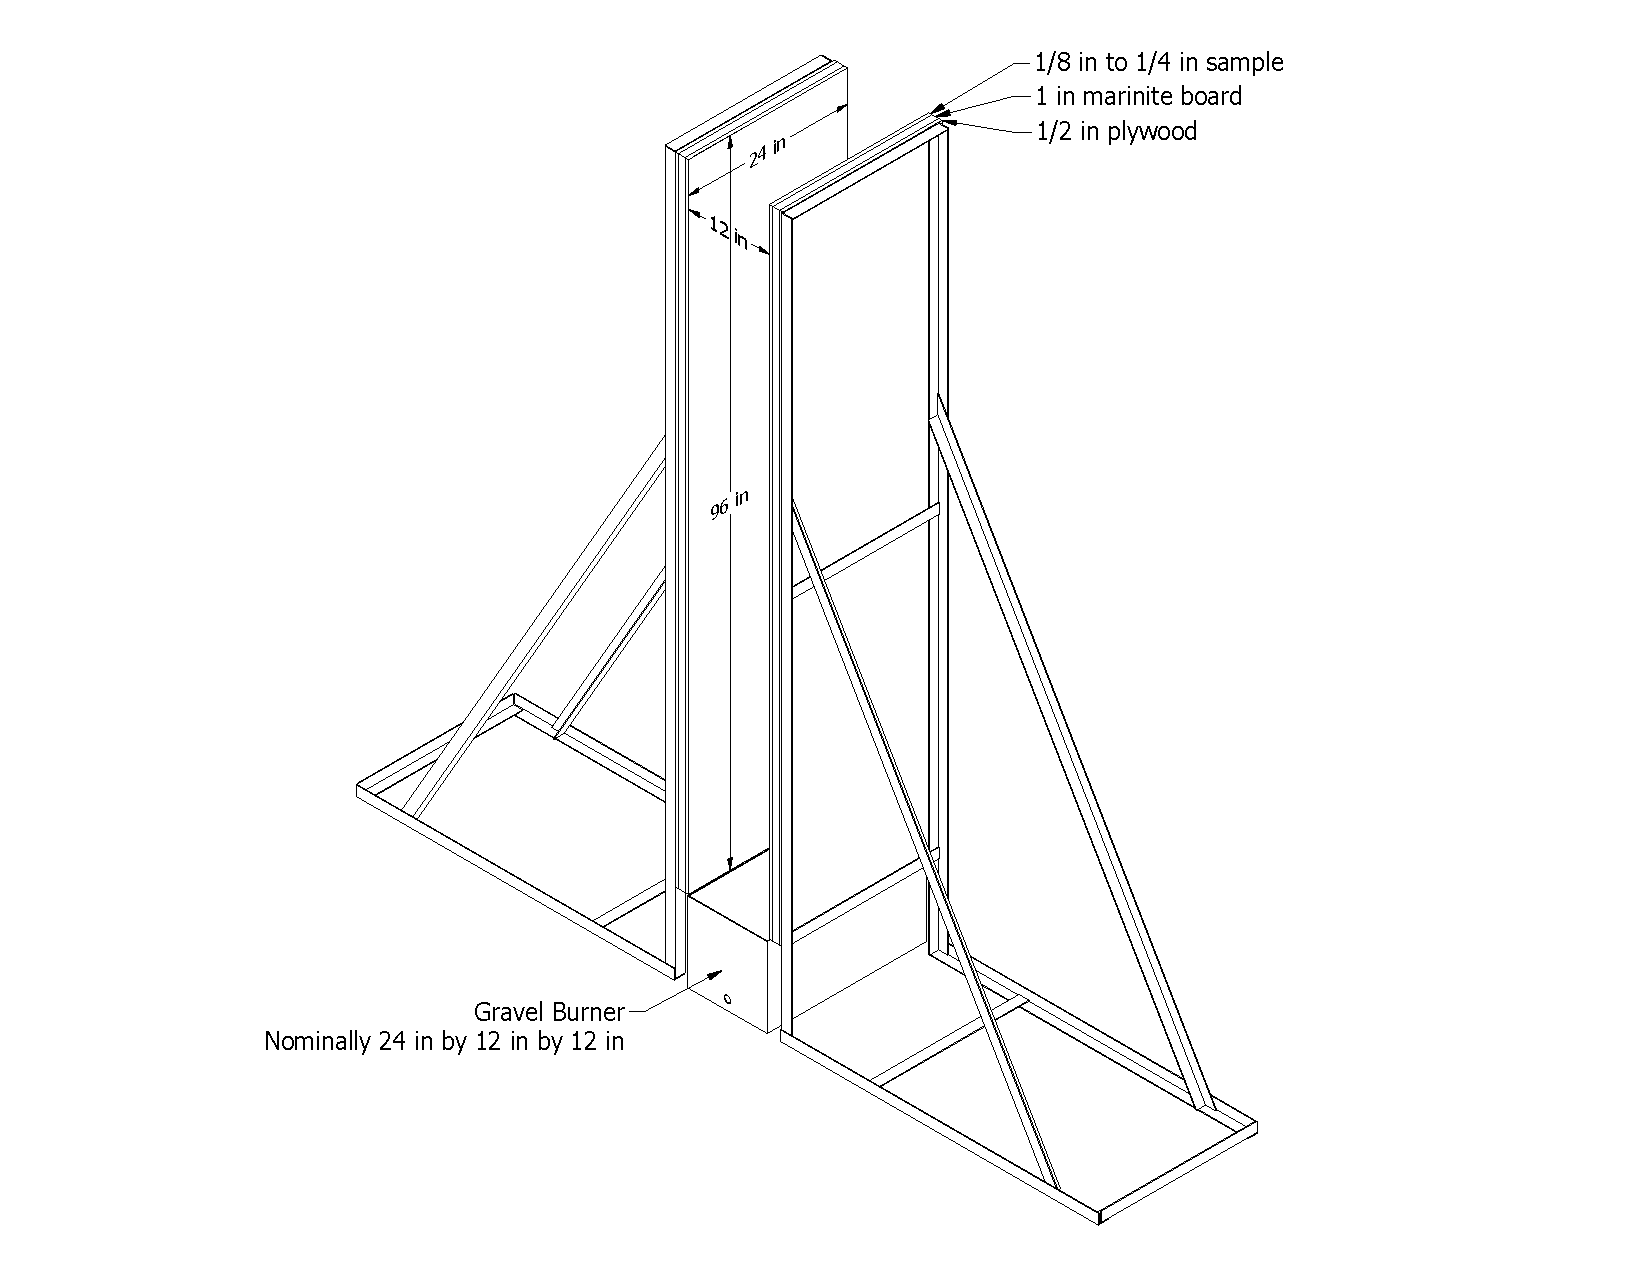
\includegraphics[width=\textwidth]{FIGURES/FM_Parallel_Panel/Full_Assembly}
\caption[Sketch of the FM parallel panel apparatus]{Sketch of the FM parallel panel apparatus.}
\label{Parallel_Panel_Sketch}
\end{figure}



\section{FM/SNL Experiments}
\label{FM_SNL_Description}


The Factory Mutual and Sandia National Laboratories (FM/SNL) test series consists of 25 compartment fire experiments conducted in 1985 for the U.S.~Nuclear Regulatory Commission (NRC) by Factory Mutual Research Corporation (FMRC), under the direction of Sandia National Laboratories (SNL)~\cite{Nowlen:NUREG4681,Nowlen:NUREG4527}. The primary purpose of these experiments was to provide data with which to validate computer models for various types of compartments typical of nuclear power plants. The experiments were conducted in an enclosure measuring approximately 18~m long by 12~m wide by 6~m high, constructed at the FMRC fire test facility in Rhode Island. A drawing is included in Fig.~\ref{FM_SNL_Drawing}. All of the experiments included forced ventilation to simulate typical power plant conditions. Six of the experiments were conducted with a full-scale control room mock-up in place. Parameters varied during the experiments included fire intensity, enclosure ventilation rate, and fire location. Only data from nineteen experiments (Tests 1-17, 21, and 22) is used in the current study. In these experiments, the fires were fueled by a propylene gas burner, and heptane and methanol liquid pools. In the experiments not selected, the heat release was not reported and could not be estimated with confidence. Table~\ref{FM_SNL_Matrix} lists the test parameters.

The following information was provided by the test director, Steve Nowlen of Sandia National Laboratory. In particular, Tests 4, 5, and 21 were given extra attention.
\begin{description}
\item[Heat Release Rate:] The HRR was determined using oxygen consumption calorimetry in the exhaust stack with a correction applied for the carbon dioxide in the upper layer of the compartment. The uncertainty of the fuel mass flow was not documented. Several tests selected for this study had the same target peak heat release rate of 516~kW following a 4~min ``t-squared'' growth profile. The test report contains time histories of the measured HRR, for which the average, sustained HRR following the ramp up for Tests 4, 5, and 21 have been estimated as 510~kW, 480~kW, and 470~kW, respectively. Once reached, the peak HRR was maintained essentially constant during a steady-burn period of 6~min in Tests~4 and 5, and 16~min in Test~21. Note that in Test 21, Nowlen reports a ``significant'' loss of effluent from the exhaust hood that could lead to an under-estimate of the HRR towards the end of the experiment.
\item[Radiative Fraction:] The radiative fraction was not measured during the experiment, but in this study it is assumed to equal 0.35, which is typical for a smoky hydrocarbons. It was further assumed that the radiative fraction was about the same in Test~21 as the other tests, as fuel burning must have occurred outside of the electrical cabinet in which the burner was placed.
\item[Measurements:] Four types of measurements were conducted during the FM/SNL test series that are used in the current model evaluation study, including the HGL temperature and depth, and the ceiling jet and plume temperatures. Aspirated thermocouples (TCs) were used to make all of the temperature measurements. Generally, aspirated TC measurements are preferable to bare-bead TC measurements, as systematic radiative exchange measurement error is reduced.
\item[HGL Depth and Temperature:] Data from all of the vertical TC trees were used when reducing the HGL height and temperature. For the majority of the tests, Sectors 1, 2, and 3 were used, all weighted evenly. For Tests 21 and 22, Sectors 1 and 3 were used, evenly weighted. Sector 2 was partially within the fire plume.
\end{description}



\begin{table}[!ht]
\caption[Summary of FM/SNL Experiments]{Summary of FM/SNL Experiments. ACH stands for Air Changes per Hour.}
\begin{center}
\begin{tabular}{|c|c|c|c|c|c|}
\hline
Test    &  Fuel             & Nominal Peak  & Fire          & Ventilation       & Room                   \\
No.     &  Type             & HRR (kW)      & Position      & Rate (ACH)        & Configuration          \\ \hline \hline
1       & Propylene Burner  &     516       & Center        & 10                & Empty                  \\ \hline
2       & Propylene Burner  &     516       & Center        & 10                & Empty                  \\ \hline
3       & Propylene Burner  &    2000       & Center        & 10                & Empty                  \\ \hline
4       & Propylene Burner  &     516       & Center        & 1                 & Empty                  \\ \hline
5       & Propylene Burner  &     516       & Center        & 10                & Empty                  \\ \hline
6       & Heptane Pool      &     500       & Wall          & 1                 & Empty                  \\ \hline
7       & Propylene Burner  &     516       & Center        & 1                 & Empty                  \\ \hline
8       & Propylene Burner  &    1000       & Center        & 1                 & Empty                  \\ \hline
9       & Propylene Burner  &    1000       & Center        & 8                 & Empty                  \\ \hline
10      & Heptane Pool      &    1000       & Wall          & 4.4               & Empty                  \\ \hline
11      & Methanol Pool     &     500       & Wall          & 4.4               & Empty                  \\ \hline
12      & Heptane Pool      &    2000       & Wall          & 4.4               & Empty                  \\ \hline
13      & Heptane Pool      &    2000       & Wall          & 8                 & Empty                  \\ \hline
14      & Methanol Pool     &     500       & Wall          & 1                 & Empty                  \\ \hline
15      & Heptane Pool      &    1000       & Wall          & 1                 & Empty                  \\ \hline
16      & Heptane Pool      &     500       & Corner        & 1                 & Empty                  \\ \hline
17      & Heptane Pool      &     500       & Corner        & 10                & Empty                  \\ \hline
21      & Propylene Burner  &     500       & Cabinet       & 1                 & Furnished              \\ \hline
22      & Propylene Burner  &    1000       & Cabinet       & 1                 & Furnished              \\ \hline
\end{tabular}
\end{center}
\label{FM_SNL_Matrix}
\end{table}



\begin{figure}[p]
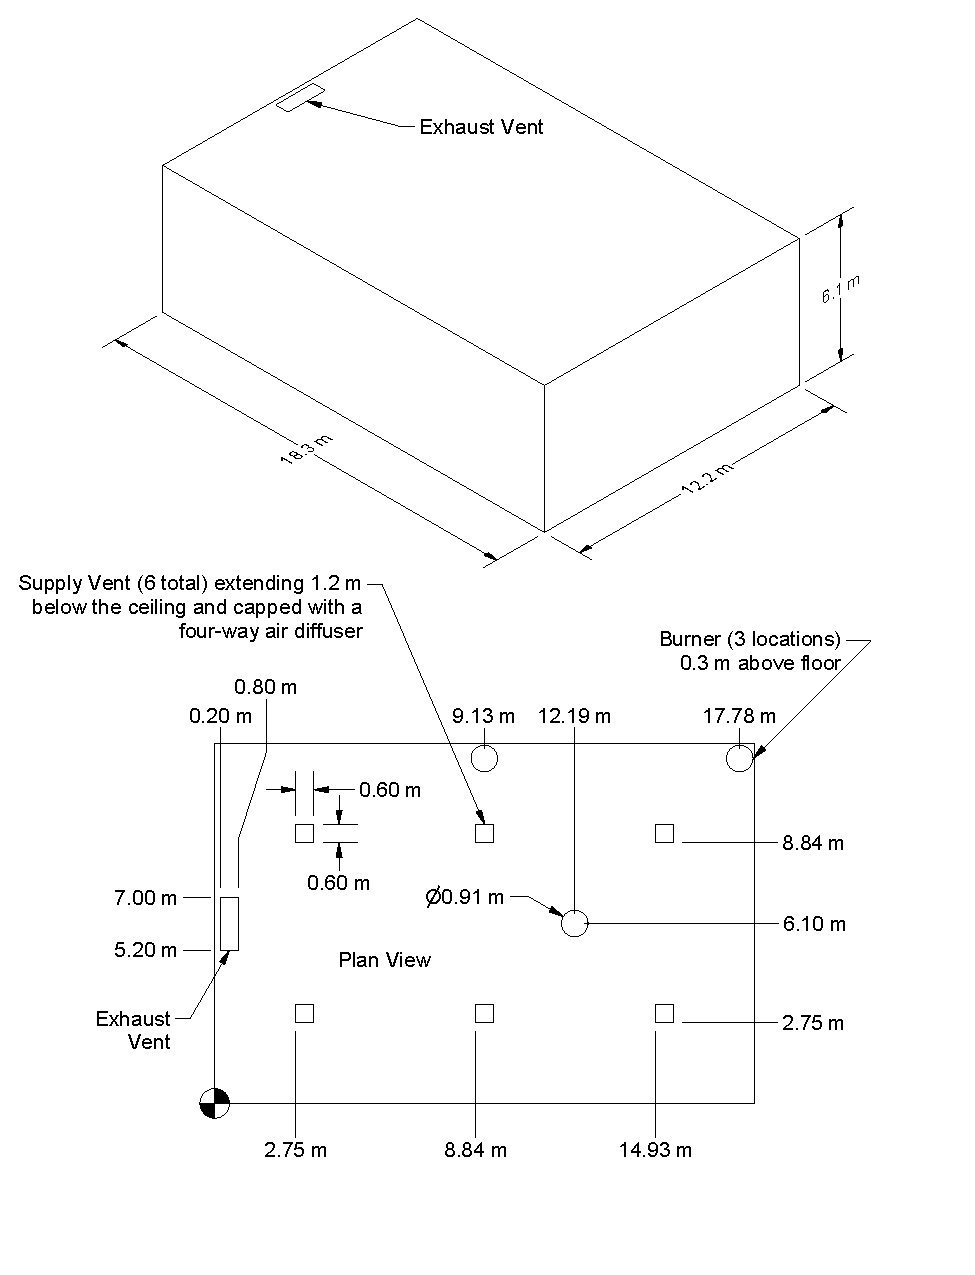
\includegraphics[width=\textwidth]{FIGURES/FM_SNL/FM_SNL_Drawing}
\caption[Geometry of the FM/SNL Experiments]{Geometry of the FM/SNL Experiments.}
\label{FM_SNL_Drawing}
\end{figure}

\FloatBarrier


%\section{FPRF/HAI Corridor Test Series}
%
%The Fire Protection Research Foundation sponsored a series of tests to evalaute the performance of smoke detection mounted in a corridor with deep beam pockets.  The test apparatus consisted of a 14.63 m (48 ft) x 3.66 m (12 ft) movable ceiling to which walls and beams could be attached.  The ceiling was instrumented with gas thermocouples along the centerline,  both at the ceiling and on the bottoms of beams, gas thermocouples along the wall and optical density meters.  21 combinations of beam depth (none, 0.3 m and 0.6 m), corridor width (1.52 m and 3.66 m), and ceiling height (2.74 m, 3.66 m, and 5.49 m) were tested.  Each ceiling height was also tested without walls to serve as an unconfined, smooth ceiling test.  Each test used an 0.3 m (1 ft) x 0.3 m, square sand burner that was centered in the corridor.  Fires were 100 kW propylene fires with a soot yield of 4.8 \% (the soot yield was measured during the test series).  A summary of the tests is shown in Table~\ref{FPRF_HAI_Matrix}.
%
%\begin{table}[h!]
%\caption{Summary of FPRF/HAI Corridor Experiments.}
%\begin{center}
%\begin{tabular}{|c|c|c|c|}
%\hline
%Test    &  Ceiling Height &  Ceiling Width &  Beam Depth  \\
%No.     &  m              &  m             &  m           \\ \hline \hline
%1,2     &  5.49           &  no walls      &  no beams    \\ \hline
%3,4     &  3.66           &  no walls      &  no beams    \\ \hline
%5,6     &  2.74           &  no walls      &  no beams    \\ \hline
%7,8     &  2.74           &  3.66          &  no beams    \\ \hline
%9,10    &  3.66           &  3.66          &  no beams    \\ \hline
%11,12   &  5.49           &  3.66          &  no beams    \\ \hline
%13,14   &  5.49           &  3.66          &  0.30        \\ \hline
%15,16   &  3.66           &  3.66          &  0.30        \\ \hline
%17,18   &  2.77           &  3.66          &  0.30        \\ \hline
%19,20   &  5.49           &  3.66          &  0.61        \\ \hline
%21,22   &  3.66           &  3.66          &  0.61        \\ \hline
%23,24   &  2.74           &  3.66          &  0.61        \\ \hline
%25,26   &  5.49           &  1.52          &  0.61        \\ \hline
%27,28   &  3.66           &  1.52          &  0.61        \\ \hline
%29,30   &  2.74           &  1.52          &  0.61        \\ \hline
%31,32   &  5.49           &  1.52          &  0.30        \\ \hline
%33,34   &  3.66           &  1.52          &  0.30        \\ \hline
%35,36   &  2.74           &  1.52          &  0.30        \\ \hline
%37,38   &  2.74           &  1.52          &  no beams    \\ \hline
%39,40   &  3.66           &  1.52          &  no beams    \\ \hline
%41,42   &  5.49           &  1.52          &  no beams    \\ \hline
%
%\end{tabular}
%\end{center}
%\label{FPRF_HAI_Matrix}
%\end{table}
%
%
%\FloatBarrier

\section{FM Vertical Wall Flame Experiments}
\label{FM_Vertical_Wall_Flame_Description}

A series of experiments was conducted by FM Global~\cite{deRis:IAFSS} in which turbulent flames were generated by flowing various gases through a vertical, water-cooled burner, 1.32~m tall and 0.38~m wide, with 0.152~m side walls. Measurements of soot depth, temperature, radiative heat flux, and radiance were made at various heights.


\section{Hamins Gas Burner Experiments}
\label{Hamins_Gas_Burner_Description}

Anthony Hamins of NIST measured the heat flux at various points around gas burner fires~\cite{Hostikka:3}. Three different sized circular burners were used, with diameters of 0.10 m, 0.38 m, and 1.0 m. Three different gases were used, acetylene, methane, and propane. The heat release rates ranged from 2~kW to 200~kW, and values of $\dot{Q}^*$ ranged from 0.04 to 10.6.


\section{Harrison Spill Plumes}
\label{Harrison_Spill_Plumes_Description}

Roger Harrison, a student at the University of Canterbury, New Zealand, performed a series of one-tenth scale experiments to characterize thermal spill plume entrainment~\cite{Harrison:2009,Harrison:IAFSS2008,Harrison:FT2007,Harrison:FSJ2010}. The dimensions of the fire compartment were 1~m by 1~m by 0.5~m high.  The height of the compartment opening was equal to the height of the compartment. The width of the opening was varied from 0.2~m to 1~m.  A 0.3~m balcony was attached to the top of the compartment opening. The balcony extended 0.5~m beyond each side of the fire compartment.  The heat release rate of the fire varied from 5~kW to 15~kW.
The plume entrainment rate was measured at different heights by varying the exhaust rate of gases from a hood above the compartment.
Two different test configurations were used to model both detached and adhered spill plumes. A diagram of the test structure is displayed in Figure~\ref{Harrison_Drawing}.

\begin{figure}[p]
\includegraphics[width=\textwidth]{FIGURES/Harrison_Spill_Plumes/Harrison_Spill_Plumes_Drawing}
\caption{Geometry of the Harrison Spill Plumes Experiments.}
\label{Harrison_Drawing}
\end{figure}




\section{Heskestad Flame Height Correlation}
\label{Heskestad_Flame_Height_Description}

A widely used experimental correlation for flame height is given by the expression~\cite{Heskestad:FSJ1983,SFPE:Heskestad}:
\be
   \frac{L_{\rm f}}{D} = 3.7 \; (\dot{Q}^*)^{2/5} - 1.02  \quad ; \quad \dot{Q}^* = \frac{\dQ}{\rho_\infty \, c_p \, T_\infty \, \sqrt{g} \; D^{5/2} }
\ee
where $\rho_\infty$, $c_p$, and $T_\infty$ are the ambient density, specific heat, and temperature. $\dot{Q}^*$ is a non-dimensional quantity that relates the fire's heat release rate, $\dQ$, with the diameter of its base, $D$. The greater the value of $Q^*$, the higher the flame height relative to its base diameter.

\section{Insulation Material Fire Resistance Tests}
\label{Insulation_Materials_Description}

Paudel et al.~\cite{Paudel:2020} studied small-scale fire resistance tests for 30 different types of stone wool insulation varying in density, thickness, and organic content. During each test, a 60~cm square sample of insulation covered by a 1~mm thick steel plate was mounted to the opening of a small combustion chamber. Thus, one side of the sample was exposed to ambient ($ T_\infty $) conditions, and the other side was attached to the steel plate whose temperature followed the ISO 834 standard fire curve,
\begin{equation}
	T_\textrm{h}(t) = T_\infty + 345 \, \textrm{log}_{10}(8t + 1)
	\label{eq:isocurve}
\end{equation}
with time, $t$, in minutes and exposure temperature, $T_{\textrm{h}}$, in $^\circ$C. The temperature measurements were made using K-type thermocouples covered with 30~mm square inorganic insulating pads. The pads were attached to the back side of the sample using heat-resistant glue or pins.

\subsubsection{Modeling Notes}

The numerical simulation is explained in Ref.~\cite{Paudel:2020}. Because detailed kinetic properties of the material are currently not available, the chemical decomposition parameters ($A$, $E_{\textrm{a}}$ and $n$) were optimized based on the cold-side measured temperatures. Unlike in Ref.~\cite{Paudel:2020}, the optimized values in the simulation are constant, $A=0.0028$~s$^{-1}$, $E_{\textrm{a}}=21700$~J/mol, and $n=0.71$. The optimization used a Monte Carlo method of 1000 Latin hypercube samples, where the sampling range was 0.001 to 1000~s$^{-1}$ for $A$, $1\times10^4$ to $1\times10^5$~J/mol for $E_{\textrm{a}}$, and 0.1 to 1 for $n$.

\section{LEMTA Spray Test for Radiation Attenuation}
\label{LEMTA_Spray_Description}

Lechene et al.~\cite{Lechene} measured the attenuation of thermal radiation passing through a water spray using a heat flux gauge. The radiation was produced by a 30~cm by 35~cm heat panel whose emission was close to a black body at 500~$^\circ$C. The horizontal distance from the radiation panel to the spray nozzle was 1.5~m and to the measurement point 3~m. The heat flux gauge was positioned at the line passing through the center of the panel. Seven nozzles were arranged in a row, 10~cm apart. They were positioned 1.5~m high. The heat panel was translated vertically during the experiment, the distance between the panel upper edge and the nozzle row varying between 20~cm and 100~cm. The attenuation of radiation is defined as previously described for the BRE Spray experiments. The purpose of the simulations is to compare the measured and simulated attenuation of radiation at different heights. The water mist nozzle has been characterized by Lechene by measuring the spray angles and the water flow rate. The droplet size is set by using a PDPA measurement in a single position, 20~cm below the injection point.


\section{LLNL Enclosure Experiments}
\label{LLNL_Enclosure_Description}

Sixty-four compartment experiments were conducted at Lawrence Livermore National Laboratory (LLNL) in 1986 to study the effects of ventilation on enclosure fires~\cite{Foote:LLNL1986}. These experiments are the basis of the Foote, Pagni, Alvares compartment temperature correlation~\cite{Foote:IAFSS1}.

The test enclosure was 6~m long, 4~m wide, and 4.5~m high (Fig.~\ref{LLNL_Enclosure_Drawing}) with a methane rock burner in the center of the space positioned at various elevations. For most of the experiments the burner was placed on the floor. The fires varied in size, $\dot{Q}$, from 50~kW to 400~kW. The burner was 0.57~m in diameter and 0.23~m height. A single door was closed and sealed for most experiments, and air was pulled through the compartment at rates, $\dot{m}$, varying from 100~g/s to 500~g/s. In some tests the enclosure included a plenum space, where make-up air could be injected from above or below. The test matrix is listed in Table~\ref{LLNL_Matrix}.

\begin{table}[p]
\caption[Summary of LLNL Enclosure Experiments]{Summary of LLNL Enclosure Experiments.}
\begin{center}
\begin{tabular}{|c|c|c|c|c|c|c||c|c|c|c|c|c|c|}
\hline
Test & Room    & $h_0$ &  $\dot{Q}$ & $\dot{m}$ & $T_\infty$ & $t_{\rm end}$  &   Test & Room    & $h_0$ &  $\dot{Q}$ & $\dot{m}$ & $T_\infty$ & $t_{\rm end}$  \\
No.  & Config. & m     &  kW        & g/s       & $^\circ$C  & s              &   No.  & Config. & m     &  kW        & g/s       & $^\circ$C  & s           \\ \hline \hline
1    & TL      & 0     & 200        & 0         & 23         & 560            &   33   & PH      & 0     & 100        & 200       & 23         & 5100        \\ \hline
2    & TL      & 0     & 200        & 0         & 27         & 545            &   34   & PH      & 0     & 100        & 300       & 34         & 4280        \\ \hline
3    & TL      & 0     & 400        & 0         & 27         & 300            &   35   & PH      & 0     & 100        & 400       & 22         & 4110        \\ \hline
4    & TL      & 0     & 300        & 0         & 24         & 385            &   36   & PH      & 0     & 100        & 500       & 29         & 4060        \\ \hline
5    & TL      & 0     & 50         & 0         & 28         & 2770           &   37   & PH      & 0     & 200        & 100       & 20         & 520         \\ \hline
6    & TL      & 0     & 100        & 0         & 29         & 1295           &   38   & PH      & 0     & 200        & 300       & 29         & 4100        \\ \hline
7    & TL      & 0     & 100        & 0         & 35         & 1240           &   39   & PH      & 0     & 250        & 100       & 18         & 430         \\ \hline
8    & TL      & 0     & 200        & 0         & 35         & 555            &   40   & PH      & 0     & 200        & 400       & 28         & 4290        \\ \hline
9    & TL      & 0     & 200        & 500       & 33         & 4220           &   41   & PH      & 0     & 150        & 100       & 20         & 970         \\ \hline
10   & TL      & 0     & 200        & 100       & 28         & 6050           &   42   & PHE     & 2     & 200        & 180       & 30         & 5120        \\ \hline
11   & TL      & 0     & 200        & 200       & 18         & 4780           &   43   & PHE     & 2     & 200        & 0         & 32         & 570         \\ \hline
12   & TL      & 0     & 200        & 300       & 21         & 5440           &   44   & PHE     & 1     & 200        & 180       & 19         & 2670        \\ \hline
13   & TL      & 0     & 200        & 400       & 28         & 5150           &   45   & PHE     & 1     & 200        & 0         & 30         & 810         \\ \hline
14   & TL      & 0     & 200        & 400       & 28         & 5090           &   46   & PHE     & 0.6   & 200        & 180       & 19         & 960         \\ \hline
15   & TL      & 0     & 100        & 300       & 24         & 4070           &   47   & PHE     & 0.6   & 200        & 0         & 19         & 730         \\ \hline
16   & TL      & 0     & 200        & 300       & 21         & 6560+          &   48   & PHE     & 0.3   & 200        & 0         & 21         & 520         \\ \hline
17   & PL      & 0     & 200        & 500       & 26         & 3980           &   49   & PHE     & 0.3   & 200        & 180       & 26         & 970         \\ \hline
18   & PL      & 0     & 200        & 400       & 21         & 4840           &   50   & PHE     & 1     & 200        & 180       & 21         & 4730        \\ \hline
19   & PL      & 0     & 200        & 300       & 18         & 5110           &   51   & PNE     & 1     & 200        & NAT       & 33         & 3360        \\ \hline
20   & PL      & 0     & 200        & 200       & 16         & 6570           &   52   & PN      & 0     & 200        & NAT       & 23         & 4680        \\ \hline
21   & PL      & 0     & 200        & 100       & 23         & 6570           &   53   & PHGS    & 0     & 200        & 185       & 33         & 1540        \\ \hline
22   & PH      & 0     & 200        & 190       & 30         & 950            &   54   & PHGS    & 0     & 200        & 215       & 21         & 4180        \\ \hline
23   & PH      & 0     & 200        & 215       & 28         & 4260           &   55   & PN      & 0     & 100        & NAT       & 31         & 4120        \\ \hline
24   & PH      & 0     & 200        & 205       & 26         & 1480           &   56   & PHGW    & 0     & 200        & 190       & 20         & 1240        \\ \hline
25   & PH      & 0     & 200        & 205       & 25         & 2050           &   57   & PHGW    & 0     & 200        & 215       & 29         & 5390        \\ \hline
26   & PH      & 0     & 200        & 500       & 24         & 4100           &   58   & PHX     & 0     & 200        & 190       & 18         & 4090        \\ \hline
27   & PH      & 0     & 200        & 100       & 23         & 540            &   59   & PHXE    & 1     & 200        & 190       & 24         & 4090        \\ \hline
28   & PH      & 0     & 150        & 150       & 31         & 1870           &   60   & PN      & 0     & 400        & NAT       & 22         & 2680        \\ \hline
29   & PH      & 0     & 250        & 250       & 28         & 1520           &   61   & TN      & 0     & 200        & NAT       & 31         & 2730        \\ \hline
30   & PH      & 0     & 250        & 300       & 34         & 4080           &   62   & TN      & 0     & 400        & NAT       & 22         & 2660        \\ \hline
31   & PH      & 0     & 250        & 500       & 36         & 4160           &   63   & TN      & 0     & 50         & NAT       & 28         & 3240        \\ \hline
32   & PH      & 0     & 100        & 100       & 33         & 4110           &   64   & TN      & 0     & 100        & NAT       & 17         & 3570        \\ \hline
\end{tabular}
\end{center}
\begin{tabbing}
\hspace{0.7in} \= T \hspace{0.2in}  \= full compartment     \hspace{0.8in} \= N \hspace{0.2in} \= natural ventilation (door open) \\
               \> P                 \> plenum configuration                \> X                \> 3 ft extension on inlet opening \\
               \> L                 \> low inlet duct                      \> GS               \> grate on inlet, north/south configuration \\
               \> H                 \> high inlet duct                     \> GW               \> grate on inlet, east/west configuration \\
               \> E                 \> elevated fire, $h_0$
\end{tabbing}
\label{LLNL_Matrix}
\end{table}

\begin{figure}[p]
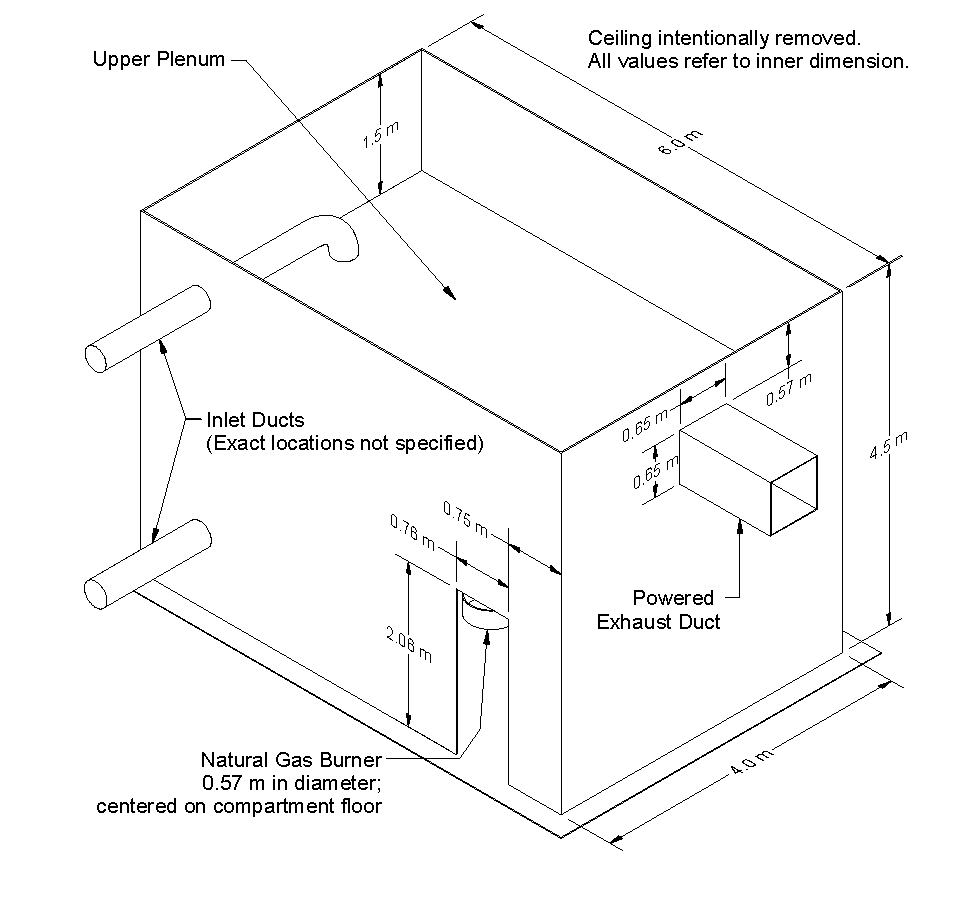
\includegraphics[width=\textwidth]{FIGURES/LLNL_Enclosure/LLNL_Enclosure_Drawing}
\caption[Geometry of the LLNL Enclosure Experiments]{Geometry of the LLNL Enclosure Experiments.}
\label{LLNL_Enclosure_Drawing}
\end{figure}

\subsubsection{Modeling Notes}

The LLNL Enclosure is modeled using a single mesh spanning the interior of the test compartment. The heat release rate of the methane burner and the thermal properties of the walls, ceiling and floor are specified based on information provided in the test report.

The test report of the LLNL Enclosure experiments lists the mass flow rate, $\dot{m}$, through the exhaust duct during the experiment. This mass flow rate is specified explicitly in the model. The make-up air into the compartment is supplied by an inlet duct and compartment leakage, both of which are modeled. The inlet duct is modeled as a 7~m long, 30~cm diameter circular duct with a loss coefficient of 25.6. The leakage area is then calculated based on the reported compartment under or over-pressures, $\Delta p$, during the experiment. The leak area is computed based on the following formulae:
\be
   \frac{\dot{m}}{\rho} = A_{\rm L} \, \sqrt{\frac{2 \, |\Delta p|}{\rho}}  \quad ; \quad A_{\rm L} = A_{\rm L,ref} \left( \frac{|\Delta p|}{|\Delta p_{\rm ref}|} \right)^{n-0.5}
\ee
The reference leakage area, $A_{\rm L,ref}$, is estimated to be 0.0033~m$^2$, $n=0.6311$, $\Delta p_{\rm ref}=50$~Pa.

In some of the experiments, the fire was reported to have self-extinguished, in which case the model employs the relatively simple Mowrer extinction model along with the one-step fast chemistry model of combustion. The Mowrer model predicts local flame extinction when the oxygen concentration within a grid cell is less than that required to raise the cell temperature to the critical flame temperature, which is 1507~$^\circ$C for methane~\cite{SFPE:Beyler}.


\section{LNG Dispersion Experiments}
\label{LNG_Dispersion_Description}

In 2006, the Fire Protection Research Foundation (FPRF) undertook a research project for the National Fire Protection Association (NFPA) Liquefied Natural Gas (LNG) Technical Committee to develop tools for evaluating LNG dispersion models. The work was carried out by the Health and Safety Laboratory (HSL), a directorate of the UK Health and Safety Executive (HSE). HSL developed the LNG Model Evaluation Protocol (MEP), which contained a structure for complete evaluation of LNG dispersion models~\cite{Ivings:HSL}. The experiments are described in Ref.~\cite{Stewart:HSL}.

\subsubsection{Modeling Notes}

The simulations of liquefied natural gas (LNG) dispersion experiments that are described in this report were originally designed by Jeffrey Engerer and Anay Luketa of Sandia National Laboratories on behalf of the Pipeline and Hazardous Materials Safety Administration of the U.S. Department of Transportation.

Parameters for the LNG dispersion experiments are given in Table~\ref{tab:LNG_Dispersion}. In some cases, values of the Monin-Obukhov parameters are taken directly from the test reports. However, for some of the experiments, these parameters were not derived using the same similarity functions as those presented above, in which case the parameters have been recomputed to best fit the measured velocity and temperature profiles. In the table, $u_*$ is the friction velocity, $\kappa=0.41$ is the Von K\'{a}rm\'{a}n constant, $z_0$ is the \emph{aerodynamic} roughness length, $\theta_*$ is the scaling potential temperature, $\theta_0$ is the ground level potential temperature, $L$ is the Monin-Obukhov length, and the similarity functions are those proposed by Dyer~\cite{Dyer:1974} and discussed in the report of the Falcon field experiments~\cite{Falcon}.

In the experiments, a fixed mass, $m$, of LNG was spilled onto water, forming a pool of increasing radius. For modeling purposes, it is assumed that the mass flux of natural gas from the circular pool is fixed at $\dot{m}''_{\rm max}=0.167$~kg/(m$^2 \cdot$s), and the temperature of the gas is $-162$~$^\circ$C, as suggested in the testing protocols. The diameter of the pool, $D$, is calculated using the assumed mass flux per unit area, the reported mass of LNG, $m$, and the spill duration, $\Delta t$.
\be
   D = \sqrt{ \frac{4 \, m}{\pi \, \dot{m}''_{\rm max} \, \Delta t} }
\ee
The values of $D$ are given in Table~\ref{tab:LNG_Dispersion}.

\begin{sidewaystable}[p]
\caption[Summary of LNG Dispersion Experiments]{Summary of LNG Dispersion Experiments.}
\begin{center}
\begin{tabular}{|l|c|c|c|c|c|c|c|c|c|c|c|c|c|}
\hline
Series                         & \multicolumn{4}{|c|}{Burro}       & \multicolumn{3}{|c|}{Coyote}  & \multicolumn{3}{|c|}{Falcon}                  & \multicolumn{3}{|c|}{Maplin Sands}          \\ \hline
Number                         & 3      & 7      & 8      & 9      &  3     & 5      & 6           &  1          & 3           & 4                 &  27             & 34             & 35      \\ \hline \hline
\multicolumn{14}{|c|}{Parameters supplied by test reports} \\ \hline
Fuel Mass, $m$ (kg)            & 14712  & 17289  & 12453  & 10730  & 6532   & 12676  & 10139       & 28074       & 21435       & 18984             & 3714            & 2094           & 3658    \\ \hline
Spill Duration, $\Delta t$ (s) & 167    & 174    & 107    & 79     & 65     & 98     & 82          & 131         & 154         & 301               & 160             & 95             & 135     \\ \hline
$p_0$ (mbar)                   & 948    & 940    & 941    & 940    & 936    & 939    & 942         & 908.9       & 900.8       & 906.3             & ---             & ---            & ---     \\ \hline
$T_0$ ($^\circ$C)              & 34.5   & 33.8   & 32.9   & 35.4   & 39.6   & 29.3   & 24.1        & 32.2        & 35.0        & 30.8              & 14.9            & 15.2           & 16.1    \\ \hline
RH (\%)                        & 5.2    & 7.4    & 4.5    & 14.4   & 11.3   & 22.1   & 22.8        & ---         & 4.0         & 12.0              & 53              & 90             & 77      \\ \hline
\multicolumn{14}{|c|}{Computed parameters} \\ \hline
$L$ (m)                        & -9.49  & -111   & 16.2   & -142   & -8.56  & -33.2  & 82.5        & 4.96        & -422        & 69.4              & -14.4           & -75.5          & -81.2   \\ \hline
$u_*$ (m/s)                    & 0.255  & 0.372  & 0.074  & 0.252  & 0.310  & 0.480  & 0.210       & 0.061       & 0.305       & 0.369             & 0.190           & 0.280          & 0.315   \\ \hline
$z_0$ (m)                      & 0.0002 & 0.0002 & 0.0002 & 0.0002 & 0.0002 & 0.0002 & 0.0002      & 0.008       & 0.008       & 0.008             & 0.0003$^\ddag$  & 0.0003$^\ddag$ & 0.0003$^\ddag$  \\ \hline
$\theta_*$ (K)                 & -0.532 & -0.097 & 0.026  & -0.035 & -0.890 & -0.520 & 0.039       & 0.058       & -0.018      & 0.152             & -0.180          & -0.075         & -0.088  \\ \hline
$\dot{q}''$ (W/m$^2$)          & -154   & -41    & 2      & -10    & -314   & -284   & 9           & 4           & -5          & 58                & -39             & -24            & -32     \\ \hline
$D$ (m)                        & 25.9   & 27.5   & 29.9   & 32.2   & 27.7   & 31.4   & 30.6        & 19.5$^\dag$ & 16.0$^\dag$ & 10.8$^\dag$       & 13.3            & 12.8           & 14.4    \\ \hline
\end{tabular}
\end{center}
$^\ddag$ The roughness length was changed to 0.00002~m to better match the measured velocity and temperature profiles

$^\dag$ The Falcon experiments involved 4 separated spills
\label{tab:LNG_Dispersion}
\end{sidewaystable}



\section{McCaffrey Plume Experiments}
\label{McCaffrey_Plume_Description}

In 1979, at the National Bureau of Standards (now NIST), Bernard McCaffrey measured centerline temperature and velocity profiles above a porous, refractory burner. There were five distinct heat release rates, ranging from 14~kW to 57~kW. The fuel was natural gas (35 kJ/L [45 MJ/kg assuming 19 kg/kgmol as mole weight for natural gas]). The burner was square, 0.3~m on each side. The results of the experiments are reported in Reference~\cite{McCaffrey:NBSIR_79-1910}. Along the centerline of the burner, velocity and temperature were measured using bi-directional probes and thermocouples, respectively.  The centerline data collapses when scaled by the Froude number as shown in Fig.~\ref{fig:McCaffrey_Correlations}. Radiant fraction measurements for natural gas were made in \cite{McCaffrey:1981}.  For convenience, we have extracted the data from that report for the heat release rates reported in \cite{McCaffrey:NBSIR_79-1910}.  See Table \ref{tab:McCaffrey_Plume_Exp}.  The burner surface temperatures are extrapolated to the surface location from a least squares fit of of the temperature data below $z/Q^{2/5} = 0.05$ \si{m.kW^{-2/5}}.  The extrapolations for each power are shown in Fig.~\ref{fig:McCaffrey_Surf_Temp}.

\begin{figure}[!ht]
\begin{tabular*}{\textwidth}{l@{\extracolsep{\fill}}r}
\includegraphics[height=2.2in]{SCRIPT_FIGURES/McCaffrey_Plume/McCaffrey_Temperature_Correlation} &
\includegraphics[height=2.2in]{SCRIPT_FIGURES/McCaffrey_Plume/McCaffrey_Velocity_Correlation} \\
\end{tabular*}
\caption[McCaffrey Plume Centerline Temperature and Velocity Correlations]
{McCaffrey Plume Centerline Temperature and Velocity Correlations (dashed lines) and raw data (symbols).}
\label{fig:McCaffrey_Correlations}
\end{figure}

\begin{table}[!ht]
\caption[Summary of McCaffrey Plume Experiments]{Summary of McCaffrey Plume Experiments, 1979.}
\begin{center}
\begin{tabular}{|c|c|c|c|c|c|}
\hline
$Q$ (kW) & $Q^*$    & $D^*$ (m)   & HRRPUA (kW/m$^2$)  & $\chi_r$ & $T_{\rm surf}$ (\si{\degreeCelsius}) \\ \hline\hline
14.4     & 0.270    & 0.178       & 160                & 0.17     & 750 \\ \hline
21.7     & 0.407    & 0.209       & 241                & 0.21     & 716 \\ \hline
33.0     & 0.618    & 0.248       & 367                & 0.25     & 630 \\ \hline
44.9     & 0.841    & 0.280       & 499                & 0.27     & 608 \\ \hline
57.5     & 1.07     & 0.309       & 639                & 0.27     & 534 \\ \hline
\end{tabular}
\end{center}
\label{tab:McCaffrey_Plume_Exp}
\end{table}

\begin{figure}[p]
\begin{tabular*}{\textwidth}{l@{\extracolsep{\fill}}r}
\includegraphics[height=2.2in]{SCRIPT_FIGURES/McCaffrey_Plume/McCaffrey_14kW_Surface_Temp} &
\includegraphics[height=2.2in]{SCRIPT_FIGURES/McCaffrey_Plume/McCaffrey_22kW_Surface_Temp} \\
\includegraphics[height=2.2in]{SCRIPT_FIGURES/McCaffrey_Plume/McCaffrey_33kW_Surface_Temp} &
\includegraphics[height=2.2in]{SCRIPT_FIGURES/McCaffrey_Plume/McCaffrey_45kW_Surface_Temp} \\
\includegraphics[height=2.2in]{SCRIPT_FIGURES/McCaffrey_Plume/McCaffrey_57kW_Surface_Temp} &
\end{tabular*}
\caption[McCaffrey Plume Burner Surface Temperatures]
{McCaffrey Plume Burner Surface Temperatures.}
\label{fig:McCaffrey_Surf_Temp}
\end{figure}



\section{NBS Multi-Room Experiments}
\label{NBS_Multi-Room_Description}

The National Bureau of Standards (NBS, which is now called the National Institute of Standards and Technology, NIST) Multi-Room Experiments consisted of 45 fire tests representing 9 different sets of conditions were conducted in a three-room suite (see Fig.~\ref{NBS_Drawing}). The experiments were conducted in 1985 and are described in detail in Ref.~\cite{Peacock:NBS_Multi-Room}. The suite consisted of two relatively small rooms, connected via a relatively long corridor. The fire source, a gas burner, was located against the rear wall of one of the small compartments.  Fire tests of 100~kW, 300~kW and 500~kW were conducted. For the current study, only three 100~kW fire experiments have been used, including Test~100A from Set~1, Test~100O from Set~2, and Test~100Z from Set~4. These tests were selected because they had been used in prior validation studies, and because these tests had the steadiest values of measured heat release rate during the steady-burn period.

Following is additional information provided by the test director, Richard Peacock of NIST:
\begin{description}
\item[Heat Release Rate:] In the two tests for which the door was open, the HRR during the steady-burn period measured via oxygen consumption calorimetry was 110~kW with an uncertainty of about 15~\%, consistent with the replicate measurements made during the experimental series and the uncertainty typical of oxygen consumption calorimetry. It was assumed that the closed door test (Test~100O) had the same HRR as the open door tests.
\item[Radiative Fraction:] Natural gas was used as the fuel in Test~100A. In Tests~100O and 100Z, acetylene was added to the natural gas to increase the smoke yield, and as a consequence, the radiative fraction increased. The radiative fraction of natural gas has been studied previously, whereas the radiative fraction of the acetylene/natural gas mixture has not been studied. The radiative fraction for the natural gas fire was assigned a value of 0.20, whereas a value of 0.30 was assigned for the natural gas/acetylene fires.
\item[Measurements:] Only two types of measurements conducted during the NBS test series were used in the evaluation considered here, because there was less confidence in the other measurements. The measurements considered here were the HGL temperature and depth, in which bare bead TCs were used to make these measurements. Single point measurements of temperature within the burn room were not used in the evaluation of plume or ceiling jet algorithms. This is because the geometry was not consistent in either case with the assumptions used in the model algorithms of plumes or jets. Specifically, the burner was mounted against a wall, and the room width-to-height ratio was less than that assumed by the various ceiling jet correlations.
\end{description}

\begin{figure}[p]
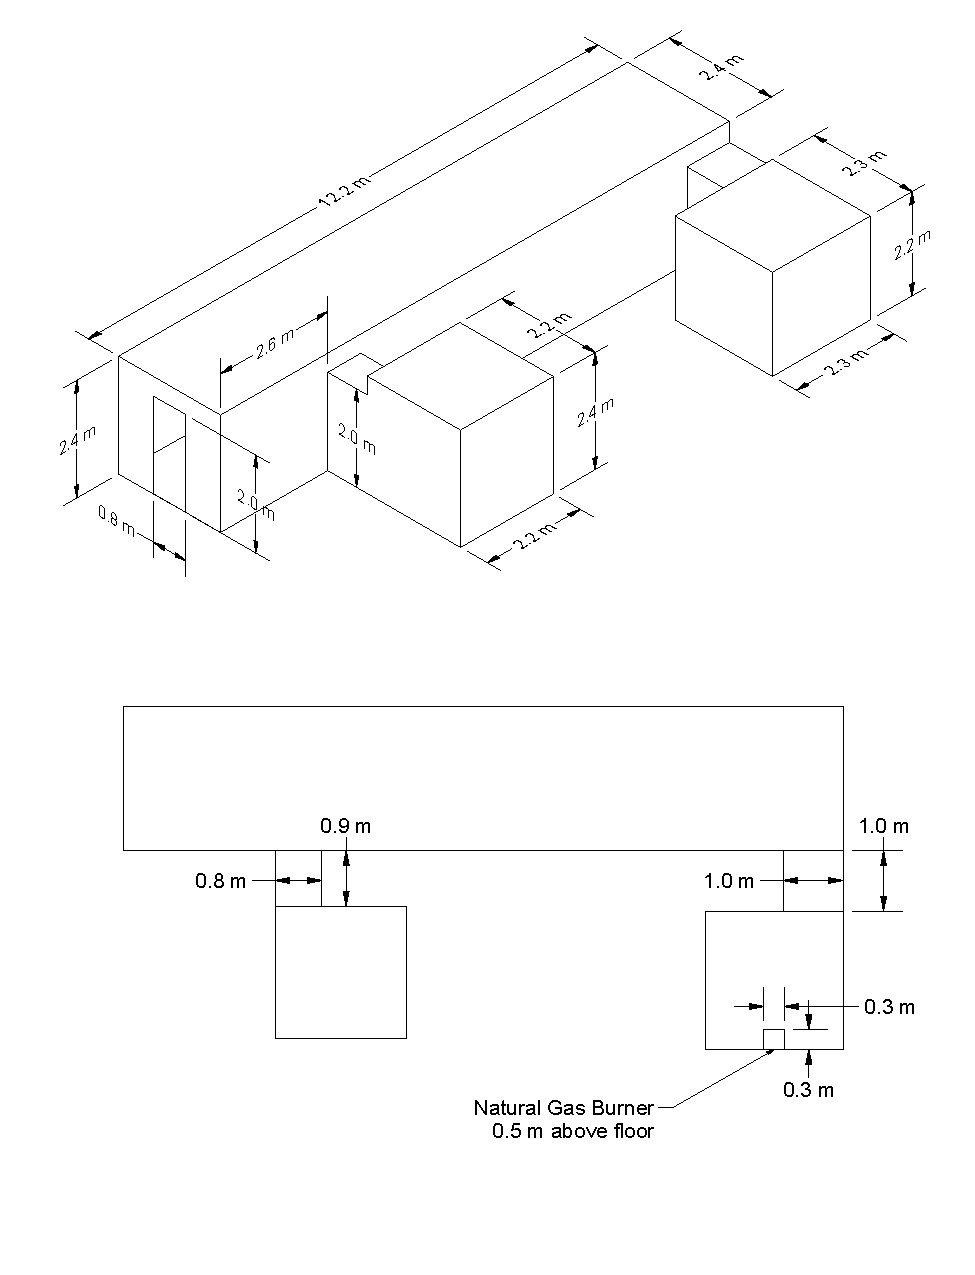
\includegraphics[width=\textwidth]{FIGURES/NBS/NBS}
\caption[Geometry of the NBS Multi-Room Experiments]{Geometry of the NBS Multi-Room Experiments.}
\label{NBS_Drawing}
\end{figure}


\section{NIST Composite Beam Experiments}
\label{NIST_Composite_Beam_Description}

A set of experiments was conducted in the Large Fire Laboratory at NIST to study the behavior of long-span steel-concrete composite floor beams designed and constructed following U.S. building codes and standards~\cite{Ramesh:TNXXXX}. The composite beam consisted of a 12.8~m long W18$\times$35 steel beam and an 16~cm thick lightweight concrete slab cast on top of 7.6~cm deep ribbed steel decking. Drawings of the compartment are shown in Figs.~\ref{NIST_Composite_Beam_Drawing_1} through \ref{NIST_Composite_Beam_Drawing_3}.

Simultaneous mechanical and fire loading was applied to the specimens. The measurements focused on evaluation of the characteristics of the fire loading, temperatures, and structural responses of the specimens to fires.

\subsubsection{Modeling Notes}

The simulations of the NIST Composite Beam experiments are performed with 5~cm grid cells and 32 meshes. The calculations are sped up by a factor of 10 using {\ct TIME\_SHRINK\_FACTOR=10}, whereby a 60~min experiment is simulated in 6~min of real time because the heat release rate is held steady for most of the experiment. The specific heats of all solid materials are reduced by a factor of 10 automatically to account for the change in time scale.

Because these experiments involve a global equivalence ratio of approximately 1, the two-step simple chemistry model is used, where soot and CO are produced when the fire becomes under-ventilated.

\begin{sidewaysfigure}[p]
\includegraphics[width=\textwidth]{FIGURES/NIST_Composite_Beam/NFRL_CompositeBeamTest_CompartmentWallLayout_1}
\caption[Elevation view of NIST Composite Beam experiments]{Elevation view of NIST Composite Beam experiments.}
\label{NIST_Composite_Beam_Drawing_1}
\end{sidewaysfigure}

\begin{sidewaysfigure}[p]
\includegraphics[width=\textwidth]{FIGURES/NIST_Composite_Beam/NFRL_CompositeBeamTest_CompartmentWallLayout_2}
\caption[Plan view of NIST Composite Beam experiments]{Plan view of NIST Composite Beam experiments.}
\label{NIST_Composite_Beam_Drawing_2}
\end{sidewaysfigure}

\begin{sidewaysfigure}[p]
\includegraphics[width=\textwidth]{FIGURES/NIST_Composite_Beam/NFRL_CompositeBeamTest_CompartmentWallLayout_3}
\caption[Side view of NIST Composite Beam experiments]{Side view of NIST Composite Beam experiments.}
\label{NIST_Composite_Beam_Drawing_3}
\end{sidewaysfigure}

\section{NIST E119 Compartment Experiments}
\label{NIST_E119_Compartment_Description}

In December 2018, three fire experiments were conducted in a compartment approximately 10.8~m wide, 7.0~m deep and 3.8~m high, constructed in the Large Fire Laboratory of NIST~\cite{Ana:TNXXXX}. The experiments were designed to test different types of floor assemblies. Two experiments, designed as replicates, lasted 15~min, and the third lasted 75~min. Four natural gas burners generated a peak heat release rate of approximately 10~MW in the 75~min experiments. The measured average upper layer gas temperature was comparable with that prescribed in the ASTM~E119 standard~\cite{E119}. Drawings of the compartment are shown in Figs.~\ref{NIST_E119_Compartment_Drawing_1} through~\ref{NIST_E119_Compartment_Drawing_3}.

\begin{sidewaysfigure}[p]
\includegraphics[width=0.65\textwidth, angle =90]{FIGURES/NIST_E119_Compartment/NIST_E119_Compartment_TCTrees}
\caption[Plan view of NIST E119 Compartment experiment]{Plan view of NIST E119 Compartment experiment.}
\label{NIST_E119_Compartment_Drawing_1}
\end{sidewaysfigure}

\begin{sidewaysfigure}[p]
\includegraphics[width=\textwidth]{FIGURES/NIST_E119_Compartment/NIST_E119_Compartment_SWall}
\caption[Elevation view of NIST E119 Compartment experiment]{Elevation view of NIST E119 Compartment experiment.}
\label{NIST_E119_Compartment_Drawing_2}
\end{sidewaysfigure}

\begin{sidewaysfigure}[p]
\includegraphics[width=\textwidth]{FIGURES/NIST_E119_Compartment/NIST_E119_Compartment_NWall}
\caption[Elevation view of NIST E119 Compartment experiment]{Elevation view of NIST E119 Compartment experiment.}
\label{NIST_E119_Compartment_Drawing_3}
\end{sidewaysfigure}

\FloatBarrier

\section{NIST Douglas Firs}
\label{NIST_Douglas_Firs_Description}

In 2009, Mell et~al. measured the burning rate of individual Douglas fir trees of various sizes and moisture contents~\cite{Mell:2009}. Nine of the trees were approximately 2~m tall, and three were approximately 5~m tall. The results were presented as averages: the three 5~m trees had an average moisture content of 26~\%, three of the 2~m trees had an average moisture content of 49~\%, and the remaining six 2~m trees had a moisture content of 14~\%. The 2~m trees were ignited with a natural gas ring burner with a diameter of 80~cm and a heat release rate of 30~kW. The trees with a moisture content of 14~\% were exposed to the burner for 10~s and the 49~\% trees were exposed for 30~s. The 5~m trees were exposed to a hexagonal burner with a span of 122~cm and HRR of 130~kW for 30~s.

\subsubsection{Modeling Notes}

The trees are modeled as a collection of cylindrical Lagrangian particles. Mell~et~al.~\cite{Mell:2009} group the particles into three size classes. The pyrolysis model assigned to the particles is described in the FDS User's Guide~\cite{FDS_Users_Guide}, chapter ``Earth, Wind and Fire,'' Section~\ref{UG-vegetation_model}, ``Thermal Degradation Model for Vegetation.''

Measured properties of the trees are listed in Table~\ref{Properties_Trees}. Generic vegetation properties are listed in Table~\ref{Assumed_Properties_Trees}. These assumed properties are typically for wood or cellulosic fuels. The moisture is modeled as water. The vegetation is assumed to be composed primarily of cellulose. Reference~\cite{Mell:2009} provides an estimate of the distribution of mass for the foliage, roundwood less than 3~mm in diameter, roundwood 3~mm to 6~mm, and roundwood 6~mm to 10~mm. For the 2~m trees, the distribution is approximately 64~\%, 11~\%, 10~\%, and 15~\%, respectively. For the 5~m trees, it is 60~\%, 17~\%, 12~\%, and 11~\%, respectively.

\begin{table}[ht]
\begin{center}
\caption[Measured properties for the NIST Douglas fir trees]{Measured properties for the NIST Douglas fir trees~\cite{Mell:2009}.}
\label{Properties_Trees}
\begin{tabular}{|l|c|c|c|c|}
\hline
Property                                & Units         & Case 1        & Case 2        & Case 3     \\ \hline \hline
Replicate Experiments                   & --            & 6             & 3             & 3          \\ \hline
Avg.~Crown Height                       & m             & 1.9           & 1.9           & 4.2        \\ \hline
Avg.~Base Height                        & m             & 0.15          & 0.15          & 0.3        \\ \hline
Avg.~Base Width                         & m             & 1.7           & 1.7           & 2.9        \\ \hline
Foliage Surface Area to Volume Ratio    & m$^{-1}$      & 3940          & 3940          & 3940       \\ \hline
Avg.~Initial Mass                       & kg            & 9.7           & 13.5          & 57.9       \\ \hline
Avg.~Moisture Fraction                  & \%            & 14            & 49            & 26         \\ \hline
Assumed Bulk Mass per Unit Volume       & kg/m$^3$      & 3.2           & 4.6           & 2.7        \\ \hline
\end{tabular}
\end{center}
\end{table}

\begin{table}
\begin{center}
\caption[Assumed properties for the vegetation]{Assumed properties for the vegetation. Note that the Pyrolysis Temperature is taken to be the temperature at which the mass loss rate peaks in the TGA experiments of Morvan and Dupuy~\cite{Morvan:CF2004}.}
\label{Assumed_Properties_Trees}
\begin{tabular}{|l|c|c|c|}
\hline
Property                        & Units                 & Value                     & Reference                             \\ \hline \hline
Chemical Composition            & --                    & C$_6$H$_{10}$O$_5$        & Assumption, Cellulose                 \\ \hline
Heat of Combustion              & kJ/kg                 & 17700                     & \cite{Susott:FS1982}                  \\ \hline
Soot Yield                      & kg/kg                 & 0.015                     & \cite{SFPE:Tewarson}                  \\ \hline
Char Yield                      & kg/kg                 & 0.26                      & \cite{Susott:FS1982}                  \\ \hline
Specific Heat                   & kJ/(kg$\cdot$K)       & 1.2                       & Various sources                       \\ \hline
Conductivity                    & W/(m$\cdot$K)         & 2                         & Assumption                            \\ \hline
Density                         & kg/m$^3$              & 514                       & \cite{Rothermel:1972}                 \\ \hline
Heat of Pyrolysis               & kJ/kg                 & 418                       & \cite{Morvan:CF2004}                  \\ \hline
Pyrolyis Temperature            & $^\circ$C             & 200                       & \cite{Morvan:CF2004}                  \\ \hline
\end{tabular}
\end{center}
\end{table}


\section{NIST Enclosure Experiments}
\label{NIST_Enclosure_Description}

A variety of reduced-scale and full-scale compartment fire experiments have been performed at NIST over the past few decades. The main objective of each series is to measure the concentrations of oxygen, carbon dioxide, carbon monoxide, soot, and unburned hydrocarbons in an under-ventilated compartment. These data sets also provide extreme temperature and heat flux measurements.

\subsection{NIST Reduced Scale Enclosure Experiments, 1994}
\label{NIST_RSE_1994_Description}

The NIST Reduced Scale Enclosure (RSE) was a 40~\% scale version of the ISO~9705 compartment~\cite{Bryner:1}. It measured 0.98~m wide by 1.46~m deep by 0.98~m tall. A door, centered on the smaller wall, was 0.48~m wide by 0.81~m tall.  A 15~cm diameter natural gas burner was positioned in the center of the compartment.  The burner was on a stand so that its top was 15~cm above the floor. The fires ranged from 50~kW to 600~kW. Species measurements, including CO concentration, were made near the ceiling in the front and back of the compartment.

\subsection{NIST Reduced Scale Enclosure Experiments, 2007}
\label{NIST_RSE_2007_Description}

Another set of reduced-scale compartment experiments was conducted in 2007 at NIST~\cite{Bundy:1}. The compartment was similar in dimension: 0.95~m wide by 1.42~m deep by 0.98~m tall with the exact same door dimensions. Four different burner types were used: a 13~cm square sand burner, a 25~cm square liquid fuel burner, a spray nozzle into 0.4~m diameter circular pan, and a 60~cm diameter circular pan. Six different fuels were used: natural gas; heptane, methanol, ethanol and toluene liquids; and solid polystyrene beads. The fires ranged from 15~kW to 425~kW, but only fires greater than 190~kW were used for comparison because the smaller fires produced no significant CO. Measurements of O$_2$, CO$_2$, CO, soot, and unburned hydrocarbon concentration were made near the ceiling in the front and back of the compartment.

\begin{table}[!ht]
\caption{Summary of NIST Reduced-Scale Experiments, 2007.}
\begin{center}
\begin{tabular}{|c|c|c|c|c|c|}
\hline
Test   &  Fuel         &  Fuel           & Peak        &  Burner       &  Doorway          \\
No.    &  Type         &  Formula        & HRR (kW)    &  Size (m$^2$) &  Opening (cm)     \\ \hline \hline
1      &  Natural Gas  &  CH$_4$         & 190         &  0.017        &  48               \\ \hline
2      &  Natural Gas  &  CH$_4$         & 395         &  0.017        &  48               \\ \hline
3      &  Natural Gas  &  CH$_4$         & 410         &  0.017        &  48               \\ \hline
4      &  Heptane      &  C$_7$H$_{16}$  & 375         &  0.063        &  48               \\ \hline
5      &  Heptane      &  C$_7$H$_{16}$  & 220         &  0.063        &  24               \\ \hline
6      &  Natural Gas  &  CH$_4$         & 420         &  0.063        &  24               \\ \hline
7      &  Heptane      &  C$_7$H$_{16}$  & 340         &  0.063        &  48               \\ \hline
10     &  Toluene      &  C$_7$H$_8$     & 340         &  0.063        &  48               \\ \hline
11     &  Ethanol      &  C$_2$H$_6$O    & 335         &  0.126        &  48               \\ \hline
12     &  Methanol     &  CH$_4$O        & 305         &  0.126        &  48               \\ \hline
15     &  Heptane      &  C$_7$H$_{16}$  & 375         &  0.126        &  48               \\ \hline
16     &  Polystyrene  &  C$_8$H$_8$     & 360         &  0.283        &  48               \\ \hline
\end{tabular}
\end{center}
\label{tab:NIST_RSE_Exp}
\end{table}


\subsection{NIST Full-Scale Enclosure Experiments, 2008}
\label{NIST_FSE_2008_Description}

The NIST FSE (2008) Experiments were conducted in an ISO~9705 compartment~\cite{Lock:1}. The compartment was 2.4~m wide by 3.6~m long by 2.4~m high with a 2~m high door at one end (Fig.~\ref{NIST_FSE_2008_Drawing}). The door width varied between 0.1~m and 0.8~m. The experiments were designed to study the effects of fuel type, fuel distribution, and vent size on under-ventilated compartment fires. Twenty-seven of the thirty experiments were simulated, which included 7 different fuels, 3 fuel sources, and 4 ventilation openings. The three experiments not simulated had several malfunctions of equipment such that the data could not be trusted.

Peak heat release rates ranged from approximately 100~kW to 2.5~MW. Table~\ref{tab:NIST_FSE_Exp} provides a summary of the experiments. Species concentrations and temperature measurements were made at the front and rear of the compartment.



\begin{figure}[!ht]
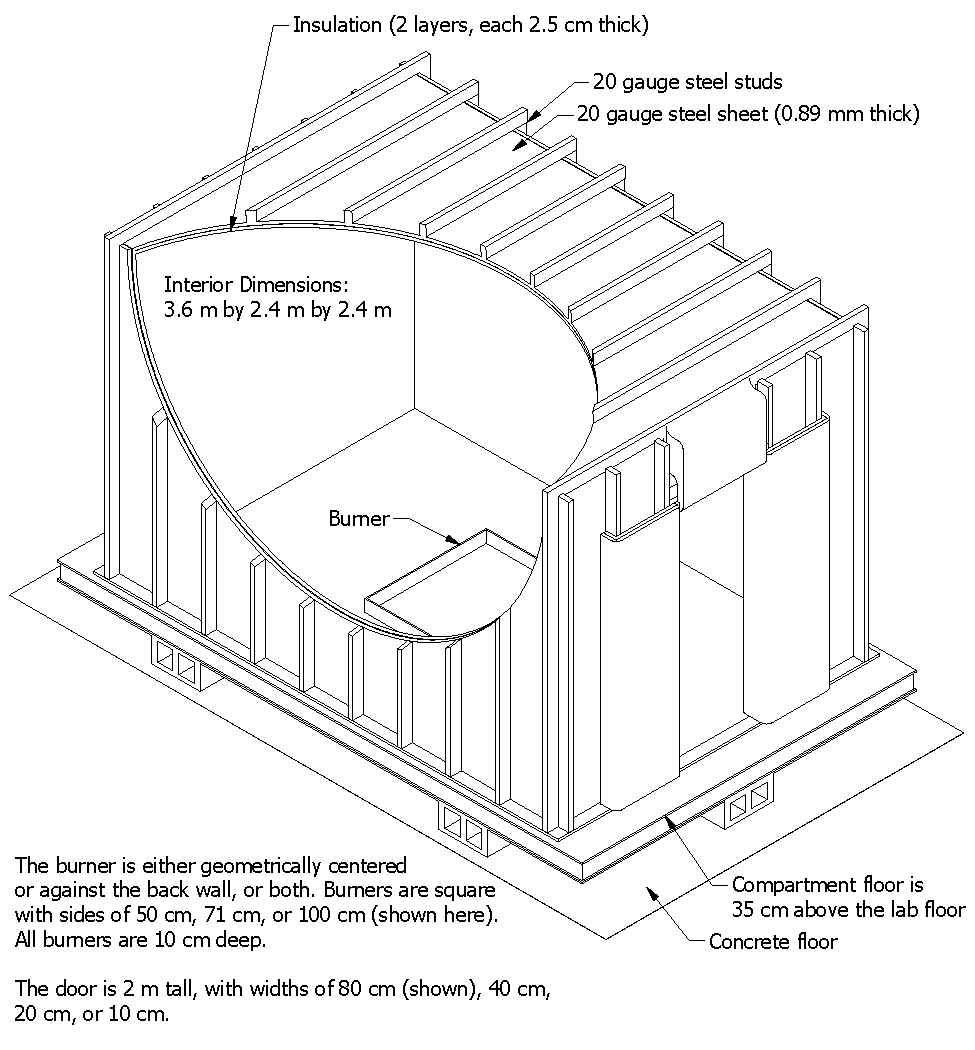
\includegraphics[width=\textwidth]{FIGURES/NIST_FSE_2008/NIST_FSE_2008_Drawing}
\caption[Geometry of the compartment used in the NIST Full-Scale Enclosure experiments]{Geometry of the compartment used in the NIST Full-Scale Enclosure (FSE) experiments.}
\label{NIST_FSE_2008_Drawing}
\end{figure}

\begin{table}[!ht]
\caption[Summary of NIST FSE Experiments selected for model validation]{Summary of NIST FSE Experiments selected for model validation.}
\begin{center}
\begin{tabular}{|l|l|c|c|c|c|c|}
\hline
Test          &  Fuel         &  Fuel             &  Fuel      &  No.~of   &  Burner       &  Doorway          \\
Name          &  Type         &  Formula          &  Mass (kg) &  Burners  &  Size (m$^2$) &  Opening (cm)     \\ \hline \hline
ISONG3        &  Natural Gas  &  CH$_4$           &            &  1        &  1.0          &  80               \\ \hline
ISOHept4      &  Heptane      &  C$_7$H$_{16}$    &  Pool Fed  &  1        &  1.0          &  80               \\ \hline
ISOHept5      &  Heptane      &  C$_7$H$_{16}$    &  Pool Fed  &  1        &  1.0          &  40               \\ \hline
ISOHept8      &  Heptane      &  C$_7$H$_{16}$    &  10        &  1        &  0.5          &  20               \\ \hline
ISOHept9      &  Heptane      &  C$_7$H$_{16}$    &  20        &  1        &  0.5          &  20               \\ \hline
ISONylon10    &  Nylon        &  C$_6$H$_{11}$NO  &  10        &  1        &  0.5          &  20               \\ \hline
ISOPP11       &  Propylene    &  C$_3$H$_6$       &  10        &  1        &  0.5          &  20               \\ \hline
ISOHeptD12    &  Heptane      &  C$_7$H$_{16}$    &  20        &  2        &  0.25         &  20               \\ \hline
ISOHeptD13    &  Heptane      &  C$_7$H$_{16}$    &  20        &  2        &  0.25         &  20               \\ \hline
ISOPropD14    &  Propanol     &  C$_3$H$_8$O      &  24        &  2        &  0.25         &  20               \\ \hline
ISOProp15     &  Propanol     &  C$_3$H$_8$O      &  24        &  1        &  0.5          &  20               \\ \hline
ISOStyrene16  &  Styrene      &  C$_8$H$_8$       &  10        &  1        &  0.5          &  20               \\ \hline
ISOStyrene17  &  Styrene      &  C$_8$H$_8$       &  30        &  1        &  1.0          &  20               \\ \hline
ISOPP18       &  Propylene    &  C$_3$H$_6$       &  20        &  2        &  0.5          &  20               \\ \hline
ISOHept19     &  Heptane      &  C$_7$H$_{16}$    &  20        &  1        &  0.5          &  20               \\ \hline
ISOToluene20  &  Toluene      &  C$_7$H$_8$       &  17        &  1        &  0.5          &  20               \\ \hline
ISOStyrene21  &  Styrene      &  C$_8$H$_8$       &  15        &  1        &  0.5          &  20               \\ \hline
ISOHept22     &  Heptane      &  C$_7$H$_{16}$    &  Spray     &  1        &  0.5          &  20               \\ \hline
ISOHept23     &  Heptane      &  C$_7$H$_{16}$    &  Spray     &  1        &  0.5          &  10               \\ \hline
ISOHept24     &  Heptane      &  C$_7$H$_{16}$    &  Spray     &  1        &  0.5          &  10               \\ \hline
ISOHept25     &  Heptane      &  C$_7$H$_{16}$    &  Spray     &  1        &  0.5          &  40               \\ \hline
ISOHept26     &  Heptane      &  C$_7$H$_{16}$    &  Spray     &  1        &  0.5          &  40               \\ \hline
ISOHept27     &  Heptane      &  C$_7$H$_{16}$    &  Spray     &  1        &  0.5          &  10               \\ \hline
ISOHept28     &  Heptane      &  C$_7$H$_{16}$    &  Spray     &  1        &  0.5          &  20               \\ \hline
ISOToluene29  &  Toluene      &  C$_7$H$_8$       &  Spray     &  1        &  0.5          &  20               \\ \hline
ISOPropanol30 &  Propanol     &  C$_3$H$_8$O      &  Spray     &  1        &  0.5          &  20               \\ \hline
ISONG32       &  Natural Gas  &  CH$_4$           &            &  1        &  0.28         &  20               \\ \hline
\end{tabular}
\end{center}
\label{tab:NIST_FSE_Exp}
\end{table}

\subsection{Modeling Notes}

In the simulations of all of the NIST enclosure experiments, it is assumed that the combustion can be simplified to two fast reactions, the first converting fuel to CO and soot, and the second converting CO and soot to CO$_2$. By default, 2/3 of the carbon in the fuel is converted to CO in the first step, the remaining 1/3 to soot. The heats of combustion for the reactions are calculated directly from the heats of formation of the individual molecules. For cases where the fuel molecule is not pre-defined in FDS (e.g., styrene), the fuel's enthalpy of formation is specified. For cases where the fuel's enthalpy of formation is not known (e.g. nylon), the heat of combustion that is reported for complete combustion is specified in a single reaction test case, from which an effective enthalpy of formation is reported\footnote{The FDS diagnostic output (.out) file contains detailed information about the reaction stoichiometry, heats of combustion, and enthalpies of formation.} and then used in the actual two-step reaction scheme.

In the experiments, the heat release rate was measured via oxygen consumption calorimetry. In the simulations, the mass loss rate of fuel was specified by taking the measured HRR and dividing by the heats of combustion listed in Ref.~\cite{SFPE:Tewarson}.

In all simulations, the model geometry included the compartment interior plus a comparable volume at the exterior to allow for a natural flow into and out of the compartment.

Also, in all simulations, the fire suppression algorithm has been turned off ({\ct SUPPRESSION=.FALSE.}). The reason for this is that the suppression algorithm is not able to distinguish viability of a fire that is close to the point of extinction. Research continues in this area.


\FloatBarrier


\section{NIST Helium Experiments}
\label{NIST_Helium_Description}

Eighteen experiments were conducted at NIST in which helium was released over a lengthy time period inside of a 1.5~m by 1.5~m by 0.75~m plexiglass box with one or two small leakage holes~\cite{Pitts:2011}. The experiments were intended to represent the release of hydrogen from passenger vehicle fuel cell inside of a residential garage. Test parameters included the release rate and length, the location of the release, and the size and location of the leakage. Measurements were made of the helium concentration in a rake at seven locations over the height of the compartment during the release and for a period of up to 11 hours post-release.

Test variables included all permutations of the leak rate and time (14.8~L/min over 3600~s or 3.71~L/min over 14400~s), leak location (on the floor at the center of the compartment, on the floor at the center of the rear wall, and 2.5~cm below the ceiling at the center of the compartment), and the leak area (2.4~cm by 2.4~cm at the center of the front wall, 3.05~cm by 3.05~cm at the center of the front wall, and a pair of 2.15~cm by 2.15~cm centered on the front wall 2.5~cm from the floor and ceiling).

Leakage areas were square holes under 10~cm$^2$ in area.  Attempting to resolve flows through these holes would have required very small grid cells in the vicinity of the holes.  Instead, the FDS HVAC model was used.  For each leakage hole a pair of HVAC ducts was defined over a height of two grid cells (one grid cell height for each vent).  Each duct was assigned one-half the leakage area and the experimentally determined orifice flow coefficient. This approach enabled bi-directional flow to occur at the leakage vent as occurred during each test following the termination of the helium release.



\section{NIST/NRC Compartment Experiments}
\label{NIST_NRC_Description}

These experiments, sponsored by the US NRC and conducted at NIST, consisted of 15 large-scale experiments performed in June 2003. All 15 tests were included in the validation study. The experiments are documented in Ref.~\cite{Hamins:SP1013-1}. The fire sizes ranged from 350 kW to 2.2 MW in a compartment with dimensions 21.7~m by 7.1~m by 3.8~m high, designed to represent a compartment in a nuclear power plant containing power and control cables. A diagram of the test structure is displayed in Figure~\ref{NIST_NRC_Drawing}.

\begin{figure}[p]
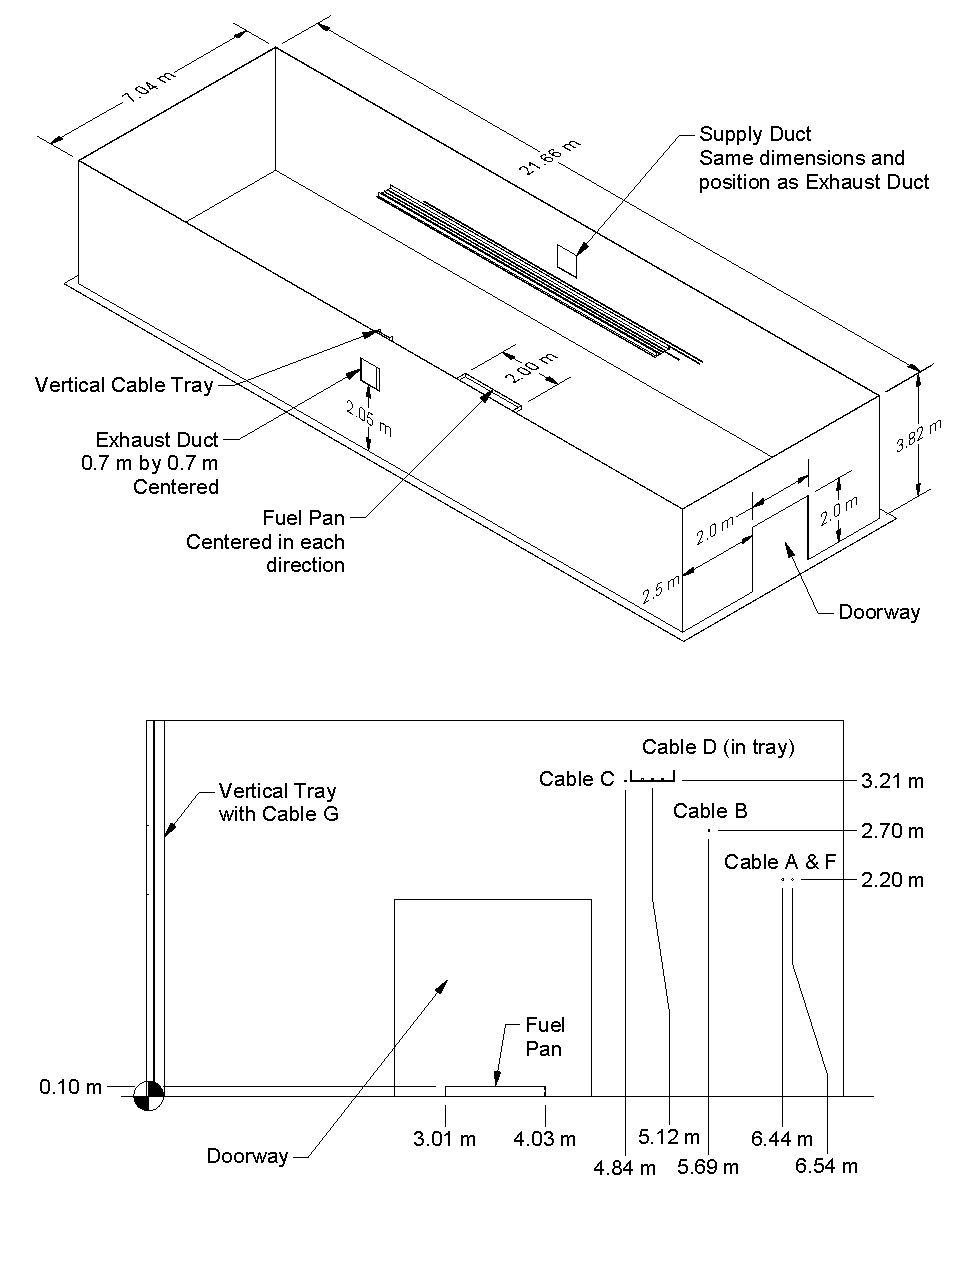
\includegraphics[width=\textwidth]{FIGURES/NIST_NRC/NIST_NRC_Drawing}
\caption[Geometry of the NIST/NRC Experiments]{Geometry of the NIST/NRC Experiments.}
\label{NIST_NRC_Drawing}
\end{figure}

The walls and ceiling were covered with two layers of marinate boards, each layer 0.0125~m thick. The floor
was covered with one layer of gypsum board on top of a layer of plywood. Thermo-physical and optical properties of the marinate
and other materials used in the compartment are given in Ref.~\cite{Hamins:SP1013-1}. The room had one door and a mechanical air injection and extraction
system. Ventilation conditions, the fire size, and fire location were varied. Numerous measurements (approximately 350 per test) were made including
gas and surface temperatures, heat fluxes and gas velocities.

Following are some notes provided by Anthony Hamins, who conducted the experiments:
\begin{description}
\item[Natural Ventilation:] The compartment had a 2~m by 2~m door in the middle of the west wall. Some of the tests had a closed door and no mechanical
ventilation (Tests 2, 7, 8, 13, and 17), and in those tests the measured compartment leakage was an important consideration. The test report lists leakage
areas based on measurements performed prior to Tests 1, 2, 7, 8, and 13. For the closed door tests, the leakage area used in the simulations was
based on the last available measurement. The chronological order of the tests differed from the numerical order.
For Test 4, the leakage area measured before Test 2 was used. For Tests 10 and 16, the leakage area
measured before Test 7 was used.
\item[Mechanical Ventilation:] The mechanical ventilation and exhaust was used during Tests 4, 5, 10, and 16, providing about 5 air changes per hour. The
door was closed during Test 4 and open during Tests 5, 10, and 16. The supply duct was positioned on the south wall, about 2~m off the floor. An
exhaust duct of equal area to the supply duct was positioned on the opposite wall at a comparable location. The flow rates through the supply and
exhaust ducts were measured in detail during breaks in the testing, in the absence of a fire. During the tests, the flows were monitored with single
bi-directional probes during the tests themselves.
\item[Heat Release Rate:] A single nozzle was used to spray liquid hydrocarbon fuels onto a 1~m by 2~m fire pan that was about 0.1~m deep. The test plan
originally called for the use of two nozzles to provide the fuel spray. Experimental observation suggested that the fire was less unsteady with the
use of a single nozzle. In addition, it was observed that the actual extent of the liquid pool was well-approximated by a 1~m circle in the
center of the pan. For safety reasons, the fuel flow was terminated when the lower-layer oxygen concentration
dropped to approximately 15~\% by volume.
The fuel used in 14 of the tests was heptane, while toluene was used for one test. The HRR was
determined using oxygen consumption calorimetry. The recommended uncertainty values
were 17~\% for all of the tests.
\item[Radiative Fraction:]  The values of radiative fraction and its uncertainty were reported as
\num{0.44 \pm 0.07} and \num{0.40 \pm 0.09} for heptane and toluene, respectively.
\item[Soot Yield:]  The values of the soot yield and its uncertainty were reported as \SI{0.0149 \pm 0.0033}{kg/kg}
and \SI{0.195 \pm 0.052}{kg/kg} for heptane and toluene, respectively.
\end{description}


\FloatBarrier

\section{NIST/NRC Corner, Wall, and Cabinet Experiments}
\label{NIST_NRC_Corner_Wall_Cabinet_Description}

In the summer of 2017, experiments were conducted in a large compartment in the NIST large fire laboratory on behalf of the U.S. Nuclear Regulatory Commission. There were two sets of experiments. In the first set, conducted in July, 2017, a natural gas burner was positioned either in a corner or against a wall, and gradually moved outward. In the second set of experiments, conducted in September, 2017, a natural gas burner was placed inside one of two steel cabinets meant to represent typical industrial-scale electrical enclosures.

The compartment for all experiments was 11~m long, 7~m wide, and 3.8~m high. The long dimension of the compartment ran east-west. A 1.8~m wide, 2.4~m high door was centered on the east (short) wall.

All of the fires were fueled by one or more 30.5~cm (1~ft) square natural gas burners. Each burner was essentially a steel box, 30.5~cm square in plan and 15~cm deep, fueled from below. The lip of the burner was 2.5~cm (1~in) wide. A 2.5~cm thick piece of Kaowool insulation was placed under a steel mesh to form the surface of the burner.

\subsection{Wall and Corner Effects}

Six large compartment experiments~\cite{McGrattan:TN1984} were conducted in July, 2017, where four natural gas burners were positioned (1) in a corner and (2) against a wall, and then moved outward in stages until the corner or wall effect became negligible. The quad burner was 60~cm by 60~cm and the burner surface was 54~cm above the floor. The corner fire was located in the southwest corner of the large compartment. The wall fire was centered on the south (long) wall.

The experiments began with the quad burner in the corner or against the wall for the first 30~min. At 30~min, the burner was moved so that its edge(s) was 10~cm away from the wall(s). It remained for 15~min, after which it was moved to 20~cm, 30~cm, 50~cm, 100~cm, and 160~cm, each time remaining 15~min for a total experiment time of 2~h.

A three-dimensional array of thermocouples was positioned on a track mounted to the ceiling above the burner. The purpose of this array was to measure maximum plume temperatures at heights of 2.1~m, 2.7~m, and 3.4~m above the floor. As the burner moved, the thermocouple array moved with it. For the corner fire experiments, when the burner was at the 0~cm, 10~cm, and 20~cm positions, the thermocouple array overhead remained at its original location in the corner. As the burner moved beyond 20~cm, the thermocouple array was moved the same amount so that the burner was always below the array in the same position. In other words, for the corner fire experiments, after the center point of the burner reached the point directly below the position 18 on the diagram below, the burner and array moved together, maintaining their relative position.

The experimental data consists primarily of thermocouple measurements. The key to the column names are as follows:
\begin{itemize}
\item TC-AG-01 through TC-AG-29 are the thermocouples at the top of the cage, 46~cm below the ceiling (see pattern below).
\item TC-BG-01 through TC-BG-29 are the thermocouples at the mid-level of the cage, 107 cm below the ceiling (see pattern below).
\item TC-CG-01 through TC-CG-29 are the thermocouples at the bottom of the cage, 168 cm below the ceiling (see pattern below).
\item TC-WT-01 through TC-WT-13 are the thermocouples of the vertical array called the West Tree. The array was 2.75 m from the west (short) wall and 3.5 m from the south (long) wall. TC-WT-01 was located 2 cm below the ceiling, and the rest were spaced 30 cm apart.
\item TC-ET-01 through TC-ET-13 are the thermocouples of the East Tree. The array was 2.75 m from the east (short) wall and 3.5 m from the south (long) wall. TC-ET-01 was located 2 cm below the ceiling, and the rest were spaced 30 cm apart.
\item TC-C-01 through TC-C-11 are the thermocouples 2 cm from the corner above the corner fire. TC-C-01 was located 2 cm below the ceiling, and the rest were spaced 30 cm apart.
\item TC-W-01 through TC-W-11 are the thermocouples 2 cm from the wall above the wall fire. TC-W-01 was located 2 cm below the ceiling, and the rest were spaced 30 cm apart.
\item HRR (cal) is the heat release rate of the fire as measured using oxygen consumption calorimetry. HRR (NG) is the heat release rate determined from the mass flow rate of natural gas.
\end{itemize}

\begin{figure}[!ht]

\begin{center}
\setlength{\unitlength}{1in}
\begin{picture}(5.5,4.5)
\multiput(0,0)(0.5,0.0){10}{\line(0,1){4.5}}
\multiput(0,0)(0.0,0.5){10}{\line(1,0){4.5}}
\multiput(0,0)(1.0,0.0){5}{\multiput(0,0)(0.0,1.0){5}{\circle*{0.075}}}
\multiput(0.5,0.5)(1.0,1.0){4}{\circle*{0.075}}
\put(0.1,0.1){1}
\put(0.1,1.1){7}
\put(0.1,2.1){13}
\put(0.1,3.1){19}
\put(0.1,4.1){25}
\put(1.1,0.1){2}
\put(1.1,1.1){8}
\put(1.1,2.1){14}
\put(1.1,3.1){20}
\put(1.1,4.1){26}
\put(2.1,0.1){3}
\put(2.1,1.1){9}
\put(2.1,2.1){15}
\put(2.1,3.1){21}
\put(2.1,4.1){27}
\put(3.1,0.1){4}
\put(3.1,1.1){10}
\put(3.1,2.1){16}
\put(3.1,3.1){22}
\put(3.1,4.1){28}
\put(4.1,0.1){5}
\put(4.1,1.1){11}
\put(4.1,2.1){17}
\put(4.1,3.1){23}
\put(4.1,4.1){29}
\put(0.6,0.6){6}
\put(1.6,1.6){12}
\put(2.6,2.6){18}
\put(3.6,3.6){24}
\put(5.25,2){\vector(0,-1){2}}
\put(5.25,2.5){\vector(0,1){2}}
\put(5.25,2.25){\makebox(0,0){0.91 m (36 in)}}
\put(2.25,-0.25){\makebox(0,0){South Wall}}
\end{picture}
\end{center}
\vspace{0.2in}
\caption[Diagram of thermocouple layout for NIST/NRC Corner Effects experiments]{Diagram of thermocouple layout for NIST/NRC Corner Effects experiments.}
\label{TC_pattern}

\end{figure}

The East and West Tree thermocouples were used to estimate the height of the hot gas layer (HGL), and the average temperatures of the upper and lower layers. Also, the three horizontal arrays of thermocouples above the burner were processed by first taking a 2~min running average of each TC, and then choosing the maximum value for each of the three elevations above the fire. These were taken as approximate centerline plume temperatures at each height. These experimental files are labelled with ``HGL'' and ``Plume'', respectively.

\subsection{Cabinet Effects}

In this second series of experiments, conducted in September, 2017, two different mock steel cabinets were used. Each cabinet was constructed of 12 gauge (2.8~mm or 7/64~in) steel plate with openings as shown in Figs.~\ref{Large_Cabinet} and \ref{Medium_Cabinet}. The large cabinet was nominally 0.9~m by 0.9~m by 2.1~m and the medium size cabinet was 0.6~m by 0.6~m by 2.1~m. The openings near the top of each cabinet were sometimes covered with a steel grill, shown in Fig.~\ref{cabinet_grill}.

\begin{figure}[p]
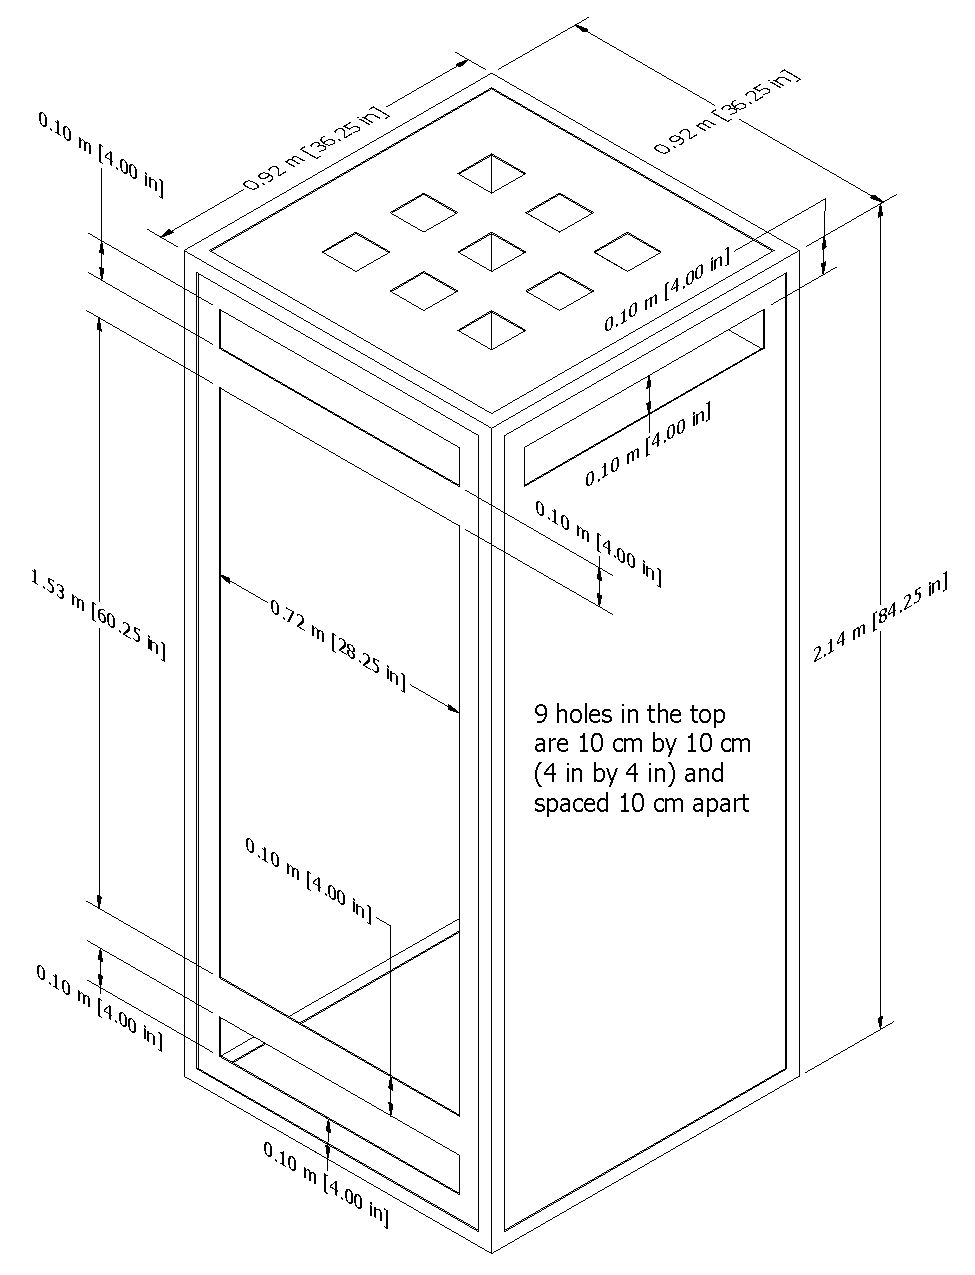
\includegraphics[width=\textwidth]{FIGURES/NIST_NRC_Corner_Effects/Cabinet_3x3x7}
\caption[Large cabinet drawing, NIST/NRC Corner Effects Experiments]{Large cabinet drawing, NIST/NRC Corner Effects Experiments.}
\label{Large_Cabinet}
\end{figure}

\begin{figure}[p]
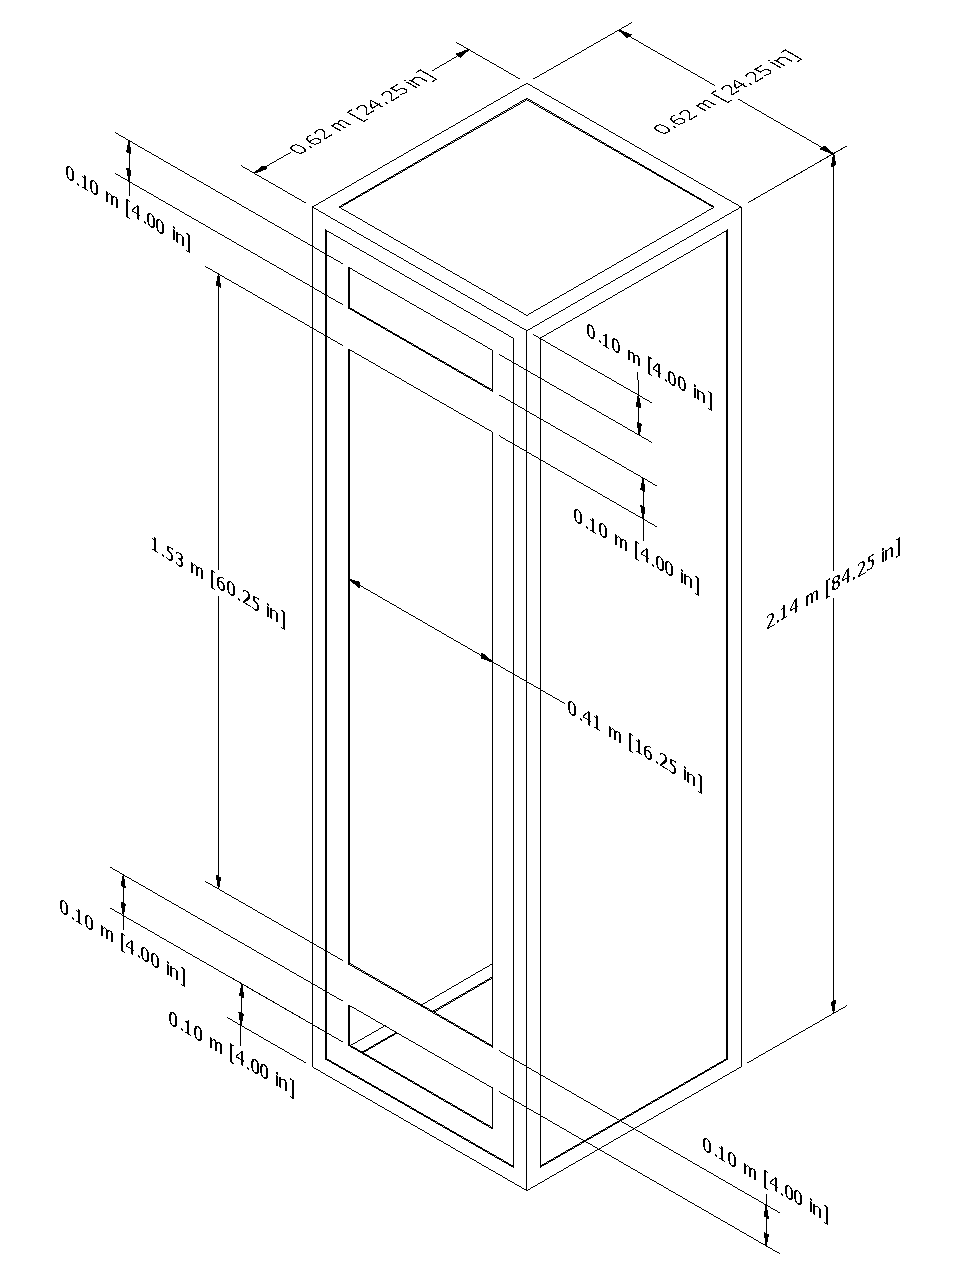
\includegraphics[width=\textwidth]{FIGURES/NIST_NRC_Corner_Effects/Cabinet_2x2x7}
\caption[Medium-sized cabinet drawing, NIST/NRC Corner Effects Experiments]{Medium-sized cabinet drawing, NIST/NRC Corner Effects Experiments.}
\label{Medium_Cabinet}
\end{figure}

\begin{figure}[!ht]
\includegraphics[width=\textwidth]{FIGURES/NIST_NRC_Corner_Effects/grill_drawing}
\caption[Cabinet grill, NIST/NRC Corner Effects Experiments]{Cabinet grill, NIST/NRC Corner Effects Experiments.}
\label{cabinet_grill}
\end{figure}


For the first set of experiments (1-6), the large cabinet was positioned with its front opening facing eastward towards the opening of the test compartment. Its left side was 1.8~m from the south wall and its front side was 5.8~m from the east wall. Two 0.3~m by 0.3~m natural gas burners were placed side by side in the cabinet from the perspective of the cabinet front opening. The top of the burner was 50~cm above the floor of the cabinet. For Tests~1-4, the front door of the cabinet was closed, and the heat release rate was initially set to 50~kW for 30~min, then it was increased to 100~kW for 15~min, 200~kW for 15~min, and 400~kW for 15~min. For Tests~5-6, the front door was opened, and the heat release rate was set to 200~kW, 400~kW, and 700~kW for 15~min each, and then 1000~kW for 5~min, a total of 50~min.

In the second set of experiments (7-10), the medium-sized cabinet was positioned so that its front was the same distance from the east wall as the large cabinet, and its left side was 2.0 m (6.5 ft) from the south wall. A single 30~cm by 30~cm gas burner was centered within. For the closed door tests, the heat release rate was 25~kW, 50~kW, 100~kW, and 200~kW, each for 15~min. For the open door tests, the heat release rate was 40~kW, 80~kW, 200~kW, and 325~kW, each for 15~min.

In the third set of experiments (11-12), the cabinet was removed, and two 30~cm by 30~cm burners were spaced 0.9~m (3~ft) apart, side to side. One of the burners was centered under the array of thermocouples. Both burners were 2.0~m from the south wall. These experiments used the same heat release rate sequence as the open and closed door large cabinet experiments.

The data files for these experiments are labelled, {\ct NIST\_NRC\_Cabinet\_Test\_n.csv}. These files contain the same measurement positions as the corner and wall experiments, with the following additional measurements:
\begin{itemize}
\item PT-1 through PT-8 are plate thermometers positioned 0.6~m (2 ft) from each side of the cabinet at heights of 0.8~m (2.5~ft) and 1.4~m (4.5~ft). PT-1 is the upper plate on the left side. PT-2 is lower left. PT-3 is upper back. PT-4 is lower back. PT-5 is upper front. PT-6 is lower front. PT-7 is upper right. PT-8 is lower right.
\item STC-1 through STC-6 are sheathed thermocouples within the cabinet, 15 cm (6 in) from the left side, centered. STC-1 is 6~cm (2.5~in) from the top. STC-2 through STC-6 are 30~cm, 60~cm, 90~cm, 120~cm, and 150~cm from the top, respectively.
\item TC-Cab is a single 24 gauge Type K thermocouple welded to the center of the back side on the outside of the cabinet. For Test~11, this TC was placed just under the Kaowool surface of the burner, and for Test~12, it was placed just above the surface.
\end{itemize}
The three dimensional array of thermocouples used in the wall and corner experiments was positioned over the front of the cabinet, such that TC positions 1, 7, 13, 19, and 25 in Fig.~\ref{TC_pattern} were just above the upper front edge of the cabinet.

The test matrix is as follows:
\begin{table}[!ht]
\caption{Summary of NIST/NRC Cabinet Experiments.}
\begin{center}
\begin{tabular}{|c|c|c|c|l|l|}
\hline
Test   & Cabinet    & Front Door & Top Vents        & Upper Side Vents                   & HRR (kW)               \\ \hline \hline
1      & Large      & Closed     & Closed           & Grill                              & 50, 100, 200, 400      \\ \hline
2      & Large      & Closed     & All open         & Grill                              & 50, 100, 200, 400      \\ \hline
3      & Large      & Closed     & Closed           & Front open, all others closed      & 50, 100, 200, 400      \\ \hline
4      & Large      & Closed     & Closed           & Front and back open, others closed & 50, 100, 200, 400      \\ \hline
5      & Large      & Open       & Closed           & Front and back open, others closed & 200, 400, 700, 1000    \\ \hline
6      & Large      & Open       & Open             & All open                           & 200, 400, 700, 1000    \\ \hline
7      & Medium     & Closed     & Closed           & Grill                              & 25, 50, 100, 200       \\ \hline
8      & Medium     & Closed     & Closed           & Open                               & 25, 50, 100, 200       \\ \hline
9      & Medium     & Open       & Closed           & Open                               & 40, 80, 200, 325       \\ \hline
10     & Medium     & Open       & Closed           & Closed                             & 40, 80, 200, 325       \\ \hline
11     & None       & N/A        & N/A              & N/A                                & 200, 400, 700, 1000    \\ \hline
12     & None       & N/A        & N/A              & N/A                                & 50, 100, 200, 400      \\ \hline
\end{tabular}
\end{center}
\label{tab:NIST_Cabinet_Experiments}
\end{table}


\FloatBarrier

\section{NIST/NRC Parallel Panel Experiments}
\label{NIST_NRC_Parallel_Panels_Description}

As part of a Nuclear Regulatory Commission (NRC) research project to assess fire behavior in electrical enclosures, rate of spread and heat release rate measurements were made on various plastics lining a parallel panel apparatus. The panels were 0.6~m (2~ft) wide, 2.4~m (8~ft) tall, and separated by 0.3~m (1~ft). A 60~kW propane sand burner was positioned at the base of the two panels. Plastics tested to date include PMMA, PVC, and PBT, cut into 6.4~mm (0.25~in) thick panels. A sketch of the apparatus, originally developed by Factory Mutual, is shown in Fig.~\ref{Parallel_Panel_Sketch}.



\section{NIST Pool Fire Experiments}
\label{NIST_Pool_Fires_Description}

The NIST Pool Fire Experiments include temperature, species concentration, and heat flux measurements of 30~cm and 100~cm diameter circular liquid fuel fires, and 37~cm gaseous burner fires.

The 30~cm burner is 15~cm deep and has a wall thickness of 1.6~mm. The burner is fitted with legs such that the burner rim is positioned 30~cm above the floor. The bottom of the burner is maintained at a constant temperature by flowing tap water (nominally 20~$^\circ$C) through a 3~cm section on the bottom of the fuel pan. The dimensions of the circular burner are similar to Weckman's methanol experiment described in Section~\ref{Waterloo_Methanol_Description}.

The 100~cm burner is also 15~cm deep, has a wall thickness of 1.6~mm, and is water-cooled.

The 37~cm burner is actually 38~cm in diameter with an effective diameter of 37~cm. It is water cooled, and the surface temperature is maintained at approximately 40~$^\circ$C.

\subsubsection{Temperature Measurements}

Hamins and Lock~\cite{Hamins:TN1928} made mean and rms centerline and radial gas temperature measurements for a 30~cm methanol pool fire. The radial measurements were made at heights of 3, 30, 40, 50, and 60~cm.

Sung et al.~\cite{Sung:TN2019} made mean and rms centerline and radial gas temperature measurements for a 100~cm methanol pool fire. The radial measurements were made at heights of 20, 60, 100, 140, and 180~cm.

\subsubsection{Gas Species Measurements}

Falkenstein-Smith et al. measured the time-averaged centerline species concentrations within the flaming region of three liquid fuel fires---acetone, ethanol, and methanol~\cite{Falkenstein-Smith:2019}. The measurements were made using a gas chromatograph/mass spectrometer system (GC/MSD). The volume fraction of each species was calculated via the number of moles identified by the GC/MSD at each centerline point. Soot mass fractions were measured during the gas sampling process.

Similar measurements were made for 37~cm diameter methane and propane fires with a measured fuel flow rate of 0.69~g/s and an estimated HRR of 34.5~kW for the methane fire, and heat release rates of 20~kW and 34~kW for the propane.

\subsubsection{Heat Flux Measurements}

Radiative and total heat flux measurements were made at various locations for the 30~cm and 100~cm methanol pool fires.
\begin{itemize}
\item Kim et al.~\cite{Kim:FSJ2019} made total heat flux measurements along a radial profile extending 1.5~m outwards from the center of the 30~cm methanol fire.
\item Hamins et al.~\cite{Hamins:CST1994} made radiative heat flux measurements along a radial profile extending from the pool center to the outer rim of the 30~cm methanol fire.
\item Klassen et al.~\cite{Klassen:GCR1994} and Kim et al.~\cite{Kim:FSJ2019} made radiative heat flux measurements along a radial profile extending outwards from the outer rim of the 30~cm methanol fire.
\item Kim et al.~\cite{Kim:FSJ2019} made total heat flux measurements along a vertical profile 60~cm from the center of the 30~cm methanol fire.
\item Sung et al.~\cite{Sung:TN2019} made total heat flux measurements along a radial profile extending from outer rim to 2~m, and at various heights and distances from center of the 100~cm methanol fire.
\end{itemize}

\subsubsection{Modeling Notes}

The 30~cm pool fires are modeled at three different grid resolutions---2~cm, 1~cm, and 0.5~cm. The 100~cm pool fires are modeled at 4~cm, 2~cm, and 1~cm resolution. The mass loss rate of the fuel is specified.

A two-step reaction mechanism is implemented. In the first reaction, fuel is converted to CO, soot, H$_2$, and H$_2$O. In the second reaction, the CO, soot, and H$_2$ are converted to CO$_2$ and H$_2$O. Both reactions employ fast kinetics, but proceed in series, not in parallel. The relative amounts of CO, soot, and H$_2$ produced in the first step are still subjects of study, and for the moment have been estimated based on measured results. For example, the methanol fire produces no measurable soot and thus all of the carbon in the fuel molecule is assumed to produce CO in the first step.

The radiative fraction is not specified, but rather predicted using the computed temperature and radiative properties computed by RadCal.


\section{NIST Smoke Alarm Experiments}
\label{NIST_Smoke_Alarm_Description}

A series of experiments was conducted by NIST to measure the activation time of ionization and photoelectric smoke alarms in a residential setting~\cite{Bukowski:1}. Tests were conducted in actual homes with representative sizes and floor plans, utilized actual furnishings and household items for fire sources, and tested actual smoke alarms sold in retail stores at that time. Thirty-six tests were conducted in two homes; 27 in a single-story manufactured home, and 8 in a two-story home. Eight experiments that were conducted in the single-story manufactured home were selected for model validation. Only tests that used a flaming ignition source with a couch or mattress fuel package were considered; the cooking oil fires and tests that used a smoldering ignition source were not considered. The flaming ignition tests used a moderate flame source to quickly ignite the fuel package.

The primary partitioning of the single-story floor plan consisted of three bedrooms, one full bathroom, one kitchen/dining area, one living room, and two hallways (see Fig.~\ref{NIST_Smoke_Alarms_Drawing}). For testing, the doors to Bedroom~3 and the bathroom were always closed. The ceiling was peaked on the long axis, reaching a height of 2.4~m. The outside walls were approximately 2.1~m in height. The slope of the ceiling was approximately 8.4$^\circ$. Groups of smoke alarms were located in the room of fire origin, at least one bedroom, and in a central location. Five stations (Station A through Station E) containing smoke alarm\footnote{Note that, in the FDS Guides, smoke detectors and smoke alarms are collectively referred to as smoke detectors because the same smoke detection algorithm is used to predict activation of either type of device.} arrays were mounted parallel to the ceiling.

Although a load cell was used in the experiments to measure the mass loss rate of the fuel package, the mass loss data were not reliable enough to reconstruct the HRR curves for each test. Instead, the HRR curves were determined by approximating the fire growth using a $t$-squared ramp, as in Eq.~(\ref{eq:t_squared}). The parameters for the $t$-squared ramp were calibrated in FDS by using the temperature measured at the highest thermocouple in the tree (2~cm below the ceiling) in the fire room.
\be
\dot Q = \dot Q_0 \left( \frac{t}{\tau} \right)^2
\label{eq:t_squared}
\ee
A time offset was used to align the predicted ceiling thermocouple temperatures with the measured temperatures. This offset is reported as the time at which the $t$-squared ramp begins. The t-squared calibration parameters and time offsets for the HRR ramps are shown in Table~\ref{tab:NIST_Smoke_Alarms_Summary}. Additionally, the ignition source had a small effect on the measured ceiling thermocouple temperatures. Therefore, the size of the ignition source was approximated as either 3~kW or 7~kW, and the time offset of the ignition source was also calibrated by using the measured ceiling thermocouple temperatures. The resulting HRR curve was input into FDS as a fire ramp. A summary of the eight tests selected for model validation is shown in Table~\ref{tab:NIST_Smoke_Alarms_Summary}.

\begin{table}[h!]
\caption[Summary of NIST Smoke Alarm Experiments selected for model validation]{Summary of NIST Smoke Alarm Experiments selected for model validation.}
\begin{center}
\begin{tabular}{|c|c|c|c|c|c|}
\hline
Test No.  &  Fire Source  &  Fire Location  &  $\dot Q_0$ (kW)  &  $\tau$ (s)  &  Time Offset (s)  \\ \hline \hline
SDC02     &  Chair        &  Living Room    &  150              &  180         &  20               \\ \hline
SDC05     &  Mattress     &  Bedroom        &  200              &  180         &  20               \\ \hline
SDC07     &  Mattress     &  Bedroom        &  350              &  180         &  50               \\ \hline
SDC10     &  Chair        &  Living Room    &  150              &  180         &  40               \\ \hline
SDC33     &  Chair        &  Living Room    &  100              &  180         &  10               \\ \hline
SDC35     &  Chair        &  Living Room    &  100              &  180         &  10               \\ \hline
SDC38     &  Mattress     &  Bedroom        &  120              &  180         &  25               \\ \hline
SDC39     &  Mattress     &  Bedroom        &  200              &  180         &  25               \\ \hline
\end{tabular}
\end{center}
\label{tab:NIST_Smoke_Alarms_Summary}
\end{table}

\begin{figure}[p]
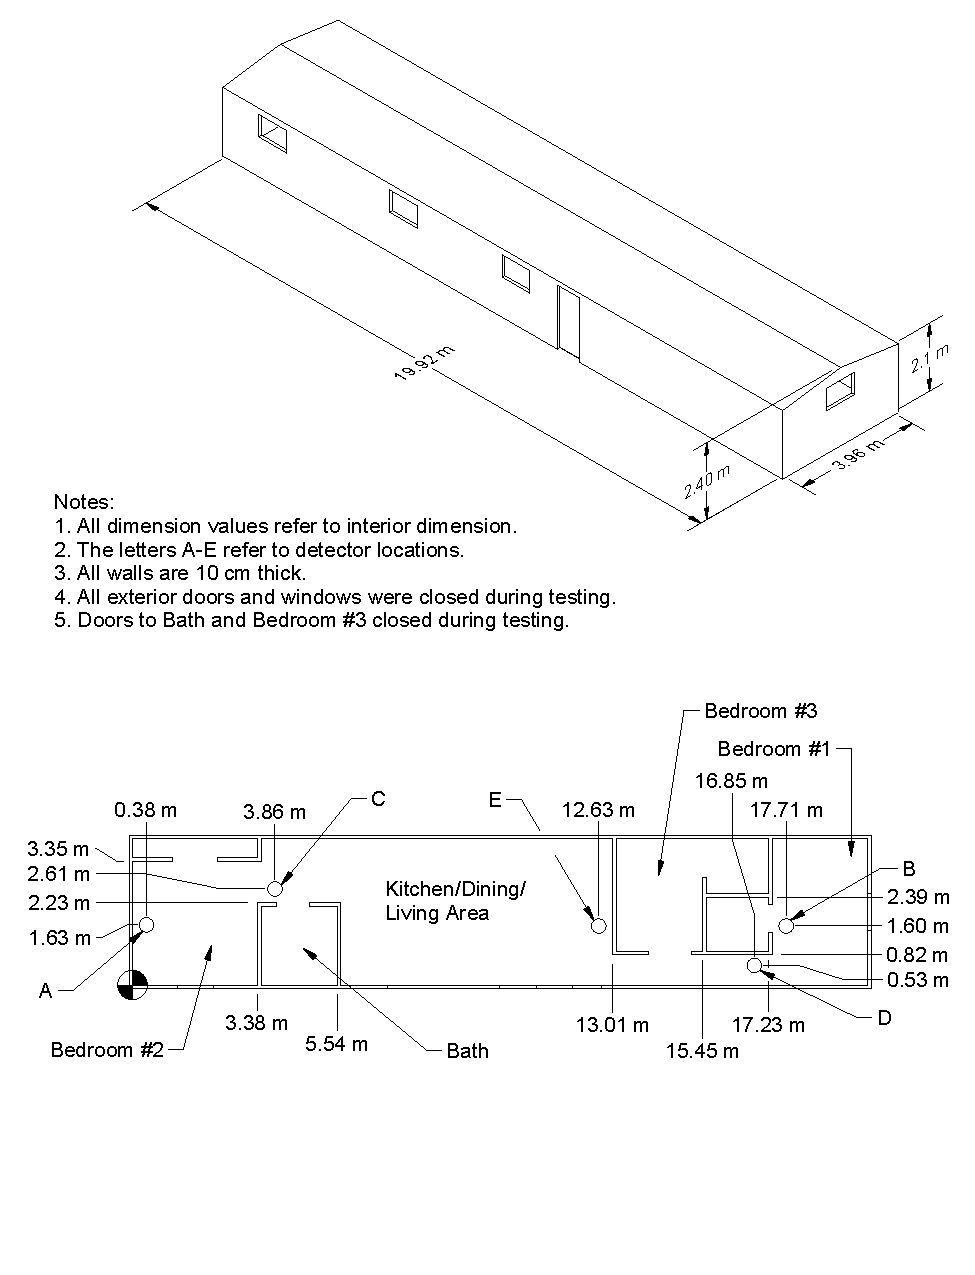
\includegraphics[width=\textwidth]{FIGURES/NIST_Smoke_Alarms/Manufactured_Home_Drawing}
\caption[Geometry of the manufactured home from the NIST Smoke Alarm Experiments]{Geometry of the manufactured home from the NIST Smoke Alarm Experiments.}
\label{NIST_Smoke_Alarms_Drawing}
\end{figure}

\FloatBarrier

\section{NIST Soot Deposition Gauge}
\label{NIST_SDG_Description}

A series of tests were performed as part of an effort to develop a gauge capable of making real time measurements of soot deposition \cite{NIST_SDG}. The test apparatus consisted of a hot plate and cold plate measuring 8 cm wide by 41~cm long and separated by 1~cm. The hot plate was electrically heated and the cold plate was water cooled. A laminar diffusion flame burner using propene as the fuel was used to generate soot. A portion of the effluent from the burner was sent through the test apparatus. In addition to tests using the new gauge, a series of gravimetric tests were performed using 47~mm diameter pieces of aluminum foil attached to the cold plate in four locations. Tests with the aluminum foil used nominal flowrates of 2.5, 5.0, and 10.0 SLPM and nominal temperature differences of 100~$^{\circ}$C and 200~$^{\circ}$C. The test channel was mounted vertically to avoid gravitational settling and with the laminar flow speeds the device essentially creates only thermophoretic deposition. Four replicate tests were performed for the 2.5 and 5.0 SLPM flowrates and three for the 10.0 SLPM flowrate. A summary of the 22 tests modeled is given in the table below.

\begin{table}[h!]
	\caption{Experiment Details for Gravimetric Measurements of Soot Deposition}
	\begin{center}
		\begin{tabular}{|c|c|c|c|}
			\hline
		Test no. & Flow Speed & $\Delta$T & Inlet Soot Conc.  \\
		         & (SLPM)     & (K)       & (mg/m$^3$)        \\ \hline \hline
		1        & 2.5        &  94       &  67.6             \\ \hline
		2        & 2.5        &  94       &  69.2             \\ \hline
		3        & 2.5        &  96       &  64.2             \\ \hline
		4        & 2.5        &  96       &  64.2             \\ \hline
		5        & 5.0        &  96       &  65.5             \\ \hline
		6        & 5.0        &  95       &  62.7             \\ \hline
		7        & 5.0        &  92       &  61.9             \\ \hline
		8        & 5.0        &  94       &  68.4             \\ \hline
		9        & 10.0       &  97       &  25.9             \\ \hline
		10       & 10.0       &  98       &  27.4             \\ \hline
		11       & 10.0       &  99       &  25.5             \\ \hline
		12       & 2.5        &  187      &  60.2             \\ \hline
		13       & 2.5        &  190      &  61.5             \\ \hline
		14       & 2.5        &  189      &  64.2             \\ \hline
		15       & 2.5        &  187      &  59.1             \\ \hline
		16       & 5.0        &  188      &  59.7             \\ \hline
		17       & 5.0        &  186      &  58.5             \\ \hline
		18       & 5.0        &  187      &  60.7             \\ \hline
		19       & 5.0        &  187      &  55.5             \\ \hline
		20       & 10.0       &  191      &  23.5             \\ \hline
		22       & 10.0       &  188      &  24.4             \\ \hline
		21       & 10.0       &  189      &  22.6             \\ \hline
		\end{tabular}
	\end{center}
	\label{tab:NIST_SDG}
\end{table}

\section{NIST Vent Study}
\label{NIST_Vent_Description}

A series of 15 reduced-scale enclosure experiments were conducted during the summer of 2017 by Summer Undergraduate Research Fellows (SURF) Fateema Farzana and Cory Schovanec. There is no test report or paper describing these experiments; only what is included here.

\subsubsection{Enclosure Geometry}
\label{Enclosure_Geometry}

A drawing of the enclosure is given in Fig.~\ref{NIST_Vent_Study_Drawing}. The enclosure consisted of two compartments stacked one on top of the other. The interior lateral dimensions of each compartment were 119~cm by 121~cm. The height of the lower compartment was 59~cm, and the upper was 61~cm. The enclosure was located within a vented laboratory space that was approximately 3~m by 3~m by 2.8~m high. The floor of this space was tiled, but a single sheet of gypsum board served as the lower floor of the test enclosure.

The front door was open in all experiments. For some portion of some of the experiments, the second floor was completely sealed. The leakage area was approximately 18~cm$^2$, measured at an over-pressure of 25~Pa.

\begin{figure}[p]
\includegraphics[width=\textwidth]{FIGURES/NIST_Vent_Study/Latex_Drawing_Plan}
\includegraphics[width=\textwidth]{FIGURES/NIST_Vent_Study/Latex_Drawing_Front}
\caption[Geometry of the compartment from the NIST Vent Study]{Geometry of the compartment from the NIST Vent Study}
\label{NIST_Vent_Study_Drawing}
\end{figure}

\subsubsection{Material Properties}

The walls, ceiling and floor of each compartment was 1.6~cm (5/8~in) Type~X gypsum board. Wood studs formed the exterior frame. Thermo-physical properties of the gypsum board were taken from in Ref.~\cite{Manzello:SiF08} and manufacturer literature. It was assumed that the specific heat was 1.089~kJ/(kg $\cdot$ K), thermal conductivity 0.15~W/m/K, and density 673~kg/m$^3$.  Additionally, a  layer of kaowool, shown in Fig.~\ref{NIST_Vent_Study_Drawing} was used to seal the gap between the removable roof and the second story walls. Aluminum tape was used to seal all other seams.

\subsubsection{Burner}

For all experiments, a 10~cm square propane burner fueled at a rate of 1.65~L/min generated a 2.5~kW fire according to the following calculation:
\be
   1.65 \frac{\rm L}{\rm min} \times \frac{1}{60} \frac{\rm min}{\rm s} \times \frac{1}{1000} \frac{{\rm m}^3}{\rm L} \times 1.967 \, \frac{\rm kg}{{\rm m}^3} \times 46,300 \, \frac{\rm kJ}{\rm kg} = 2.50 \; {\rm kW}
\label{Conversion_Equation}
\ee
Note that the mass flow controller (Sierra Instruments SmartTrak~50) assumed standard conditions to be 0~$^\circ$C and 101325~Pa. For Tests~13-15, a Dwyer flow meter was used in place of the mass flow controller. The flow meter had a flow range of 4~L/min air.

\subsubsection{Thermocouples}

Eight Type-K thermocouples were inserted at each level to measure the vertical temperature profile. The thermocouples formed a vertical array at 84~cm from the left wall of the enclosure, and 17~cm from the front wall. TC-1 was defined as the uppermost thermocouple, with heights defined as the vertical distance from the compartment specific floor.

\begin{table}[h!]
\caption{Heights of the thermocouples above the floor of each level of the enclosure}
\begin{center}
\begin{tabular}{|c|c|c|c|c|c|c|c|c|c|c|c|c|c|c|c|c|}
\hline
Floor 2 TC's   & 1& 2& 3 & 4& 5& 6& 7&8\\ \hline
Height (cm) & 56.5& 50.8& 45.5& 41.0& 36.0& 29.8& 19.8& 10.5\\ \hline
Floor 1 TC's & 9&10&11&12&13&14&15&16\\ \hline
Height (cm) &51.8&47.0&40.64&35.6&30.48&25.7& 16.5&7.0\\ \hline


\end{tabular}
\end{center}
\label{Tab.TC}
\end{table}

\subsubsection{Test Procedure}

Each experiment lasted 100~min with a 5~min cool down period. Table~\ref{tab:NIST_Vent_Study} indicates the times when vents and windows were opened after the start of each experiment. For Test No. 1-4, two trials were performed. In each case, the difference in temperature remained within 3 percent, a difference of less than 1~$^\circ$C. For this reason, no further replicates were conducted.

\begin{table}[h!]
\caption{Vent State by Experiment: Time Opened}
\begin{center}
\begin{tabular}{|c|c|c|c|c|c|c|c|c|c|}
\hline
Test & Front    & Left    & Right     & Left     & Right   & Left         & Right        & Right   & Roof    \\
No.  & Window   & Window  & Window    & Vent     & Vent    & Vent Area    & Vent Area    & Vent    & Vent    \\
     & (min)    & (min)   & (min)     & (min)    & (min)   & (cm$^2$)     & (cm$^2$)     & Shape   & (min)   \\ \hline \hline
1    & 0        &  0      &  0        &  Closed  &  0      &  0           &  100         &  Square & Closed  \\ \hline
2    & 0        &  0      &  0        &  Closed  &  20     &  0           &  100         &  Square & Closed  \\ \hline
3    & 60       &  40     &  Closed   &  Closed  &  20     &  0           &  100         &  Square & Closed  \\ \hline
4    & 0        &  0      &  0        &  Closed  &  0      &  0           & 400          &  Square & Closed  \\ \hline
5    & 0        &  0      &  0        &  Closed  &  20     &  0           &  400         &  Square & Closed  \\ \hline
6    & 60       &  40     &  Closed   &  Closed  &  20     &  0           &  400         &  Square & Closed  \\ \hline
7    &  0       &  0      &  0        &  0       &  0      &  100         &  400         &  Square & Closed  \\ \hline
8    &  0       &  0      &  0        &  20      &  40     &  100         &  400         &  Square & Closed  \\ \hline
9    &  80      &  60     &  Closed   &  20      &  40     &  100         &  400         &  Square & Closed  \\ \hline
10   &  0       &  0      &  0        &  Closed  &  0      &  0           &  100         & Circle  & Closed  \\ \hline
11   &  0       &  0      &  0        &  Closed  &  20     &  0           &  100         & Circle  & Closed  \\ \hline
12   &  60      &  40     &  Closed   &  Closed  &  20     &  0           &  100         & Circle  & Closed  \\ \hline
13   &  0       &  0      &  0        &  0       &  0      &  100         &  400         &  Square & 0       \\ \hline
14   &  0       &  0      &  0        &  20      &  40     &  100         &  400         &  Square & 60      \\ \hline
15   &  Closed  & Closed  &  Closed   &  20      &  40     &  100         &  400         &  Square & 60      \\ \hline
\end{tabular}
\end{center}
\label{tab:NIST_Vent_Study}
\end{table}


\FloatBarrier

\section{NRCC Facade Heat Flux Measurements}
\label{NRCC_Facade_Description}

A series of experiments was conducted by the Fire Research Section of the Institute for Research in Construction, National Research Council of Canada (NRCC), to measure the heat flux to a mock exterior building facade due to a fire within a compartment~\cite{Oleszkiewicz:ASME,Oleszkiewicz:FireTech}. The experiments selected for model validation were conducted using a series of propane line burners within a compartment whose interior dimensions were 5.95~m wide, 4.4~m deep, and 2.75~m high (see Fig.~\ref{NRCC_Facade_Drawing}). There were five different door/window sizes:
\begin{enumerate}
\item 0.94 m by 2.00 m high
\item 0.94 m by 2.70 m high (door)
\item 2.60 m by 1.37 m high (shown in Fig.~\ref{NRCC_Facade_Drawing})
\item 2.60 m by 2.00 m high
\item 2.60 m by 2.70 m high (door)
\end{enumerate}
There were four fire sizes: 5.5~MW, 6.9~MW, 8.6~MW, and 10.3~MW. In all, 19 experiments were conducted, with the exception of the 10.3~MW fire with Window~1. In each experiment, heat flux measurements were made 0.5~m, 1.5~m, 2.5~m, and 3.5~m above the top of the door/window.

\begin{figure}[p]
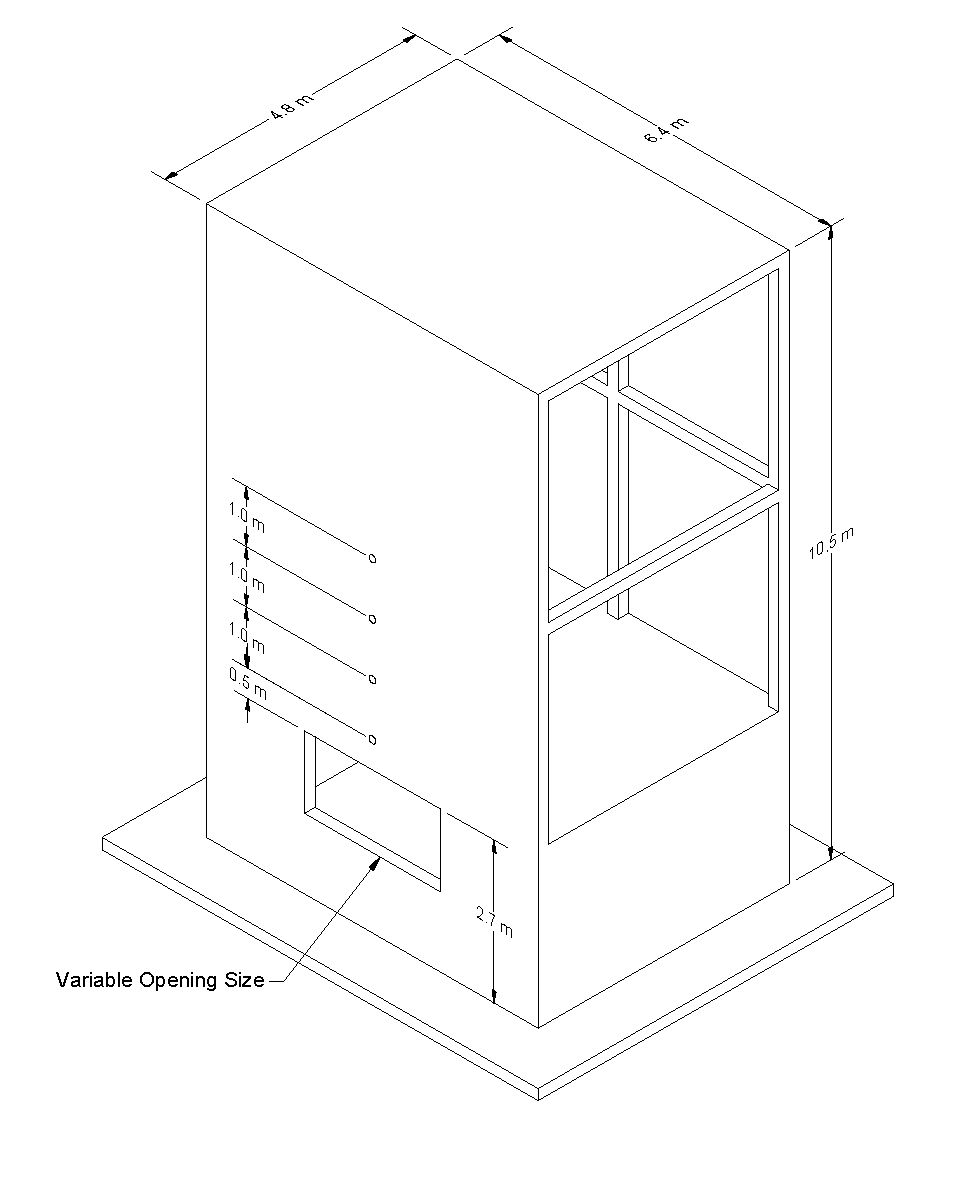
\includegraphics[width=\textwidth]{FIGURES/NRCC_Facade/NRCC_Facade}
\caption[Geometry of the NRCC Facade Experiments]{Geometry of the NRCC Facade Experiments.}
\label{NRCC_Facade_Drawing}
\end{figure}


\section{NRCC Smoke Tower Experiments}
\label{NRCC_Smoke_Tower_Description}

In 2006 and 2007, the National Research Council of Canada (NRCC) conducted 10 fire experiments in a 10 story experimental facility in Almonte, Ontario to study smoke movement through the stair shaft to the upper floors of the building. Four of these experiments utilized actual commodities as fuel, and six utilized a propane burner. Four of the six propane fires were intended to reproduce the heat release of the commodity fires, and these experiments (BK-R, CMP-R, CLC-I-R, and CLC-II-R) have been chosen for this guide. Details of the experiments are included in a master's thesis and paper by Yan Wang~\cite{Wang:Thesis,Wang:FT2011}. A description of FDS simulations of the propane experiments not included in this guide is given by Hadjisophocleous and Jia~\cite{Hadjisophocleous:FT2009}. The analysis of the propane burner experiments discussed in this guide are based on the work of Paul Tyson at Ulster University as part of his master's thesis~\cite{Tyson:Thesis}.

\begin{figure}[p]
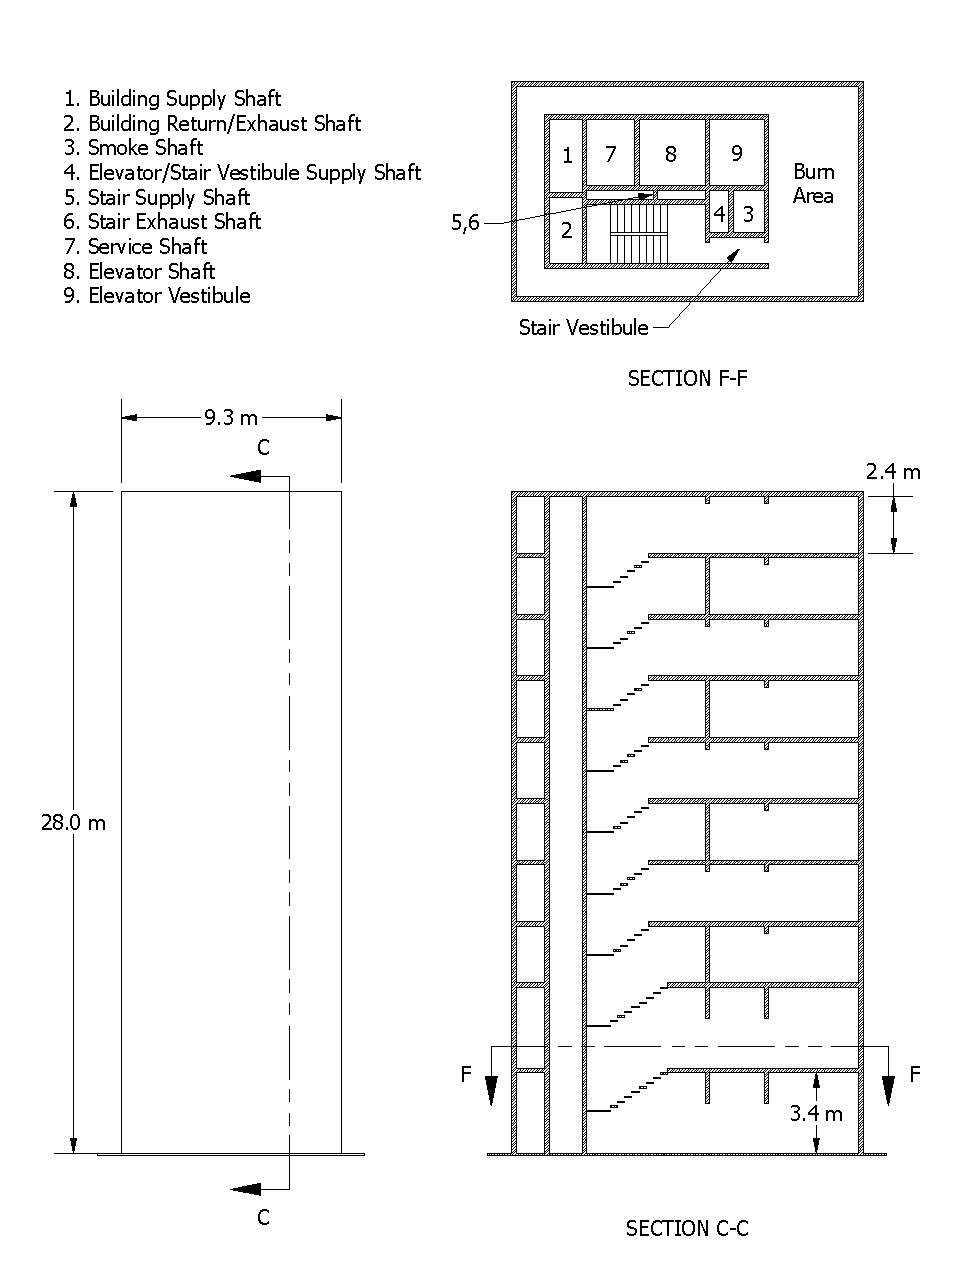
\includegraphics[width=\textwidth]{FIGURES/NRCC_Smoke_Tower/NRCC_Smoke_Tower}
\caption[Geometry of the NRCC Smoke Tower Experiments]{Geometry of the NRCC Smoke Tower Experiments.}
\label{NRCC_Smoke_Tower_Drawing}
\end{figure}

The tower was designed as a test bed for the center core of a high-rise building. It includes a compartment and corridor on each floor, a stair shaft, elevator shaft and service shafts~\cite{Achakji:1987}. Figure~\ref{NRCC_Smoke_Tower_Drawing} displays the geometry of the building as modeled in FDS. All walls and floor slabs are taken to be 0.2~m thick. The first two floors are 3.4~m high, slab to slab. The upper eight floors are 2.4~m, slab to slab. The propane burner was located on the second floor and the smoke flowed through open doors to the stair vestibule and stair shaft itself. In the four experiments considered in this guide, the stair shaft was open on the fourth, sixth, eighth, and tenth floors. The other floors were closed off to the stair shaft. The ventilation system was turned off. A single door was opened on the first floor, and there were no other openings to the outside save natural building leakage. The referenced documents do not explicitly include estimates of leakage areas, but for the sake of modeling, the leakage for each floor was concentrated at a single 1.5~m by 1.5~m exterior window. The leakage area was specified based on an estimate of a ``loose'' building exterior in NFPA~92~\cite{NFPA_92}. This is a very important consideration in modeling because it determines the extent to which the smoke rising up the stair shaft encounters an opposing downward flow.

Thermocouples and gas analyzers were placed at various locations to measure temperature and O$_2$, CO$_2$ and CO concentrations. A vertical array of TCs was located in the fire compartment and the doorway leading into the stair shaft on the second floor. TCs were also placed at each floor in the stair shaft. The gas analyzers were located in the stair shaft at the second floor, just outside the door to the fire compartment.



%\section{NRL Confined Space Experiments}
%
%The U.S. Naval Research Laboratory (NRL) performed a multi-year series of experiments inside of a four level,
%23 compartment test facility with 20 doors and ceiling vents whose exterior boundaries were airtight~\cite{Confined_JFPE} ~\cite{Confined_DTIC}.
%Three HVAC systems were installed in the facility: a supply air system that takes suction from a fan room and discharges the air to the each of the compartments,
%an exhaust system that takes suction from each of the compartments and discharges it to the fan room, and a smoke control control system that takes suction from an upper
%level compartment and discharges it to the ambient (see Figure~\ref{confined_HVAC}).
%A second set of HVAC ducts directly connected the second level with the fourth level (see Figure~\ref{confined_bypass}).
%
%\begin{figure}[ht]
%\begin{center}
%%\includegraphics[width=5.in]{FIGURES/NRL_Confined_Space/confined_space_hvac_layout}
%\end{center}
%\caption{Confined space HVAC system layouts.}
%\label{confined_HVAC}
%\end{figure}
%
%\begin{figure}[ht]
%\begin{center}
%%\includegraphics[width=5.in]{FIGURES/NRL_Confined_Space/confined_space_bypass}
%\end{center}
%\caption{Confined space bypass ducts.}
%\label{confined_bypass}
%\end{figure}
%
%The test facility was instrumented with gas thermocouples, surface thermocouples, optical density meters, gas sampling lines (CO$_2$, CO, and O$_2$),
%and velocity probes in a small number of doors, vents, and HVAC ducts.  Test variables included the number of opened doors and hatches, the number of vent openings to the ambient,
%the fire location, the fire size, and the operation of the HVAC systems.  All the fires were marine diesel pool fires.
%
%\FloatBarrier


\section{NRL/HAI Wall Heat Flux Measurements}
\label{NRL_HAI_Description}

Back, Beyler, DiNenno and Tatem~\cite{Back:IAFSS4} measured the heat flux from 9 different sized propane fires set up against a wall composed
of gypsum board. The experiments were sponsored by the Naval Research Laboratory and conducted by Hughes Associates, Inc., of Baltimore, Maryland. The
square sand burner ranged in size from 0.28~m to 0.70~m, and the fires ranged in size from 50~kW to 520~kW.

\section{PRISME Project}
\label{PRISME_Description}

PRISME is the name of a fire test program conducted under the auspices of the Organization for Economic Cooperation and Development, Nuclear Energy Agency (OECD/NEA). The experiments were conducted at the French Institut de radioprotection et de s\^{u}ret\'{e} nucl\'{e}aire (IRSN) at Cadarache. A variety of experiments were conducted to study ventilation effects, electrical cable failure, and leakage. The test reports are not publicly available, but an entire edition of {\em Fire Safety Journal} documented various experimental and modeling studies~\cite{Audouin:FSJ}.

The PRISME DOOR series consisted of six experiments, five of which involving two compartments connected by an open door (Tests 1-5) and one involving a third compartment (Test 6). The compartments were 5~m by 6~m by 4~m high. A well-instrumented ventilation system supplied air and exhausted combustion products at specified rates, but the thermal expansion of the gases caused these rates to change, a phenomenon that was intended to test the ventilation capabilities of the models. Wahlqvist and van Hees~\cite{Wahlqvist:FSJ} modeled these experiments using FDS and contributed the input files for the cases documented in this guide.

The PRISME LEAK series consisted of experiments where smoke and heat flowed through various types of leaks between the test compartments. Instrumented cables were placed at various locations, and gas and solid phase temperatures were measured. FDS was used to simulate the heating up of the cables using the measured gas temperature several centimeters from the cables~\cite{Dreisbach:Interflam}.

\section{Purdue Flames}
\label{Purdue_Flames_Description}

A turbulent buoyant diffusion flame is established on a diffuser burner with an exit diameter of 7.1 cm. The diverging angle of the burner is 7$^\circ$ such that the gaseous fuel (methane) is decelerated and forms a uniform velocity distribution at the burner exit \cite{Xin:CF2005}. The methane (CH4) mass flow rate (84.3 mg/s) The buoyant diffusion flame burns in a quiescent atmospheric pressure environment. The flame is surrounded by a screened enclosure to minimize flame disturbance. The Froude number of the flame is 0.109 and matches that of a 7.1 cm diameter liquid toluene pool fire \cite{Xin:CF2005,Zhou:CS1998}. The total heat release rate of the methane flame is 4.2 kW under the assumption of complete combustion, and the visible flame height is approximately 36 cm \cite{Xin:CF2005}. Measured and computed vertical and horizontal velocity, mixture fraction, and temperature values for this flame have been reported by Xin et al.~\cite{Xin:CF2005,Xin:PhD2002} and Zhou et al.~\cite{Zhou:CS1998,Zhou:PurduePhD1999}. The mean temperatures have been inferred from the measured species concentrations \cite{Xin:CF2005} by assuming an adiabatic flame. The interdependencies between species concentrations, temperature and specific heat have been ignored for determining the mean temperature.

\section{Ranz Marshall Droplet Experiments}
\label{Ranz_Marshall_Description}

In 1952 Ranz and Marshall performed a set of droplet evaporation experiments that ultimately led to the development of the Ranz-Marshall Nusselt and Schmidt number correlations for droplet heat and mass transfer~\cite{Ranz}. The experiments documented in Figure 8 and Tables 1 to 4 in the paper have been modeled with FDS. For the experiment in Figure 8 of the Ranz and Marshall paper a 1043~$\mu$m water droplet was suspended in still dry air at an ambient temperature and pressure of 24.9$^\circ$C and 98792 Pa. The droplet diameter was measured over time. For the experiments in Tables 1 to 4 in the paper, droplets were suspended in a dry air stream. Experimental parameters included the type of fluid (water or benzene), the initial drop diameter, the ambient temperature, and the velocity of the air stream. The evaporation rate in the FDS simulations was determined by allowing the drop temperature to reach equilibrium and then using the time it took the drop to decrease in size to 350~$\mu$m (the minimum reported droplet size in Figure 8 of the paper). The table below summarizes the experiments.

\begin{table}[h]
	\caption[Summary of Ranz and Marshall droplet evaporation experiments]{Summary of Ranz and Marshall droplet evaporation experiments.}
	\begin{center}
		\begin{tabular}{|c|c|c|c|c|c|c|}
			\hline
			Table   & Test   & Fluid  &  Diameter  &  Air Temperature & Pressure &  Velocity  \\
			No.     & No.    &        & ($\mu$m)   &  ($^{\circ}$C)   &  (Pa)    &  (m/s)     \\ \hline \hline
1 & 1 & Water & 954 & 19.9 & 99059 & 2.46 \\hline
1 & 2 & Water & 954 & 24.6 & 98659 & 2.1 \\hline
1 & 3 & Water & 954 & 24.9 & 98659 & 1.723 \\hline
1 & 4 & Water & 954 & 25.3 & 98659 & 1.532 \\hline
1 & 5 & Water & 954 & 25.4 & 98659 & 1.197 \\hline
1 & 6 & Water & 954 & 24.3 & 98392 & 0.952 \\hline
1 & 7 & Water & 954 & 24.4 & 98392 & 0.762 \\hline
1 & 8 & Water & 954 & 24.5 & 98392 & 0.571 \\hline
1 & 9 & Water & 954 & 24.5 & 98392 & 0.571 \\hline
1 & 10 & Water & 954 & 24.6 & 98392 & 0.285 \\hline
1 & 11 & Water & 954 & 24.7 & 98392 & 0.1513 \\hline
1 & 12 & Water & 954 & 24.8 & 98392 & 0.1718 \\hline
1 & 13 & Water & 954 & 24.9 & 98392 & 0.0841 \\hline
1 & 14 & Water & 954 & 25.0 & 98392 & 0.0337 \\hline
1 & 15 & Water & 954 & 23.2 & 98392 & 2.86 \\hline
1 & 16 & Water & 954 & 23.6 & 99459 & 2.67 \\hline
1 & 17 & Water & 954 & 23.7 & 99459 & 2.28 \\hline
1 & 18 & Water & 954 & 24.0 & 99459 & 3.06 \\hline
1 & 19 & Water & 954 & 24.9 & 98792 & 0 \\hline
2 & 1 & Water & 950 & 90.0 & 98792 & 2.3 \\hline
2 & 2 & Water & 950 & 77.5 & 98792 & 1.1 \\hline
2 & 3 & Water & 950 & 78.7 & 98792 & 1.1 \\hline
2 & 4 & Water & 950 & 78.7 & 98792 & 1.1 \\hline
2 & 5 & Water & 950 & 84.0 & 98792 & 1.83 \\hline
2 & 6 & Water & 950 & 82.5 & 98792 & 1.14 \\hline
2 & 7 & Water & 950 & 83.0 & 98792 & 1.14 \\hline
2 & 8 & Water & 950 & 66.4 & 98792 & 0.55 \\hline
2 & 9 & Water & 950 & 71.4 & 98792 & 0.176 \\hline
3 & 1 & Water & 850 & 115.0 & 98792 & 1.84 \\hline
3 & 2 & Water & 710 & 115.0 & 98792 & 1.84 \\hline
3 & 3 & Water & 560 & 85.0 & 98792 & 0.188 \\hline
3 & 4 & Water & 460 & 85.0 & 98792 & 0.188 \\hline
3 & 5 & Water & 960 & 221.0 & 98792 & 1.84 \\hline
3 & 6 & Water & 580 & 221.0 & 98792 & 1.84 \\hline
3 & 7 & Water & 880 & 193.0 & 98792 & 0.77 \\hline
3 & 8 & Water & 600 & 193.0 & 98792 & 0.77 \\hline
3 & 9 & Water & 1010 & 125.0 & 98792 & 0.21 \\hline
4 & 1 & Benzene & 1100 & 24.4 & 97592 & 0.051 \\hline
4 & 2 & Benzene & 1100 & 26.4 & 97592 & 0.153 \\hline
4 & 3 & Benzene & 1100 & 27.1 & 98125 & 0.289 \\hline
4 & 4 & Benzene & 1100 & 17.9 & 98525 & 0.748 \\hline
4 & 5 & Benzene & 1100 & 17.5 & 98525 & 1.124 \\hline
4 & 6 & Benzene & 1100 & 17.7 & 97725 & 1.5 \\hline
4 & 7 & Benzene & 1100 & 20.7 & 97725 & 0.188 \\hline
4 & 8 & Benzene & 1100 & 20.4 & 97725 & 0.283 \\hline
4 & 9 & Benzene & 1100 & 19.9 & 97725 & 0.755 \\hline
4 & 10 & Benzene & 1100 & 20.0 & 97725 & 1.13 \\hline
4 & 11 & Benzene & 1100 & 20.2 & 97725 & 1.516 \\hline
4 & 12 & Benzene & 1100 & 20.2 & 97725 & 1.9 \\hline
4 & 13 & Benzene & 1100 & 20.4 & 97725 & 2.88 \\hline
		\end{tabular}
	\end{center}
	\label{Ranz_Marshall_Summary}
\end{table}

\section{Restivo Compartment Air Flow Experiment}
\label{Restivo_Description}

Velocity measurements for forced airflow within a 9~m by 3~m by 3~m high compartment (Fig.~\ref{Restivo_Drawing}) were made by Restivo~\cite{Restivo:1979}. These measurements have been widely used to validate CFD models designed for indoor air quality applications. It was also used to assess early versions of FDS~\cite{Emmerich:1,Emmerich:2,Musser:1}. In the experiment, air was forced into the compartment through a 16.8~cm vertical slot along the ceiling running the width of the compartment with a velocity of 0.455~m/s. A passive exhaust was located near the floor on the opposite wall, with conditions specified such that there was no buildup of pressure in the enclosure. The component of velocity in the lengthwise direction was measured in four arrays: two vertical arrays located 3~m and 6~m  from the inlet along the
centerline of the room, and two horizontal arrays located 8.4~cm above the floor and below the ceiling, respectively. These measurements were taken using hot-wire anemometers. While data on the specific instrumentation used are not readily available, hot-wire systems tend to have limitations at low velocities, with typical thresholds of approximately 0.1~m/s.

\begin{figure}[ht]
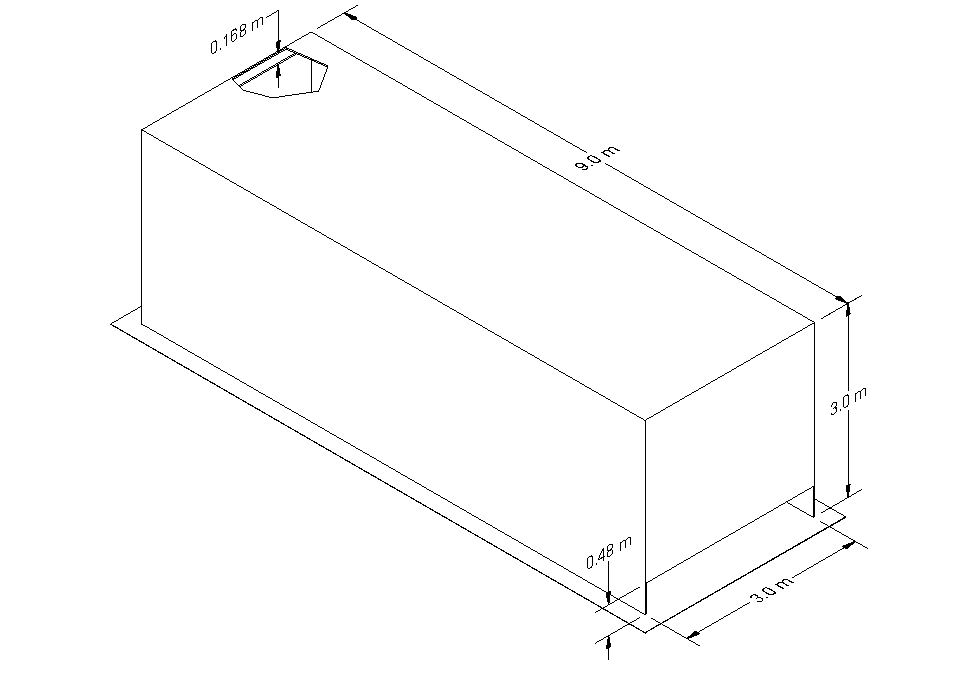
\includegraphics[width=\textwidth]{FIGURES/Restivo_Experiment/Restivo_Drawing}
\caption[Geometry of Restivo's compartment]{Geometry of Restivo's compartment.}
\label{Restivo_Drawing}
\end{figure}

\section{Sandia Plume Experiments}
\label{Sandia_Plume_Description}

The Fire Laboratory for Accreditation of Models by Experimentation (FLAME) facility \cite{OHern:2005,Blanchat:2001} at Sandia National Laboratories in Albuquerque, New Mexico, is designed specifically for validating models of buoyant fire plumes.  The plume source is 1 m in diameter surrounded by a 0.5 m steel `ground plane'. PIV/PLIF techniques are used to obtain instantaneous joint scalar and velocity fields.  O'Hern et al.~\cite{OHern:2005} studied a turbulent buoyant helium plume in the FLAME facility. Earlier work to model this experiment has been performed by DesJardin et al.~\cite{DesJardin:2004}. Tieszen et al.~\cite{Tieszen:2004,Tieszen:2002} studied methane and hydrogen pool fires.

\section{SETCOM Wall Condensation Experiments}
\label{SETCOM_Cond_Description}
The Separate Effect Test for Condensation Modeling (SETCOM) facility is located in J\"{u}lich, Germany \cite{setcom_cfd}. The facility is a recirculating duct containing a flow conditioning section for establishing temperature and humidity and a test section for performing condensation experiments. The condensation section contains a 4~m or 5~m long, water-cooled, aluminum plate for its floor with the remaining walls adiabatic. The condensation section can be tilted from horizontal to vertical to investigate the effects of orientation on condensation. A set of five experiments were performed using the 4~m test section that measured the condensation heat flux from hot, high humidity air. Temperature, humidity, and flow rate were varied.

\subsection{Modeling notes}
Prior to running the validation cases, a set of five scoping simulations were run with no condensation. These simulations used a short length of the test section with {\ct PERIODIC} boundary conditions. These cases were used to determine the rms velocity as a function of the mean velocity.

The condensation simulations included a 4~m portion of duct upstream to allow for flow development, and a 1 m portion of duct downstream to avoid boundary effects on the test section. The upstream boundary condition was set with the conditions shown in the table below along with synthetic eddy method inputs using the rms velocity determine from the scoping simulations. The outlet was defined as an {\ct OPEN} boundary. The experiments measured temperature 1.5~cm into the aluminum plate along the plate centerline. The test measured condensation heat transfer was used with the inside plate temperature to derive the plate surface temperature. The condensation plate {\ct TMP\_FRONT} was set to derived temperature as a function of length along the plate.

\begin{table}[h]
	\caption[Summary of SETCOM condensation experiments selected for model validation]{Summary of SETCOM condensation experiments selected for model validation.}
	\begin{center}
		\begin{tabular}{|c|c|c|c|}
			\hline
			Test      &  Air Speed        &  Temperature          &  Humidity             \\
			No.       &  (m/s)            &  ($^{\circ}$C)        &  (\%)                 \\ \hline \hline
			1         &  0.8              &  86                   &  69                   \\ \hline
			2         &  1.8              &  84                   &  57                   \\ \hline
			3         &  3.7              &  79                   &  59                   \\ \hline
			4         &  4.2              &  78                   &  71                   \\ \hline
			5         &  5.2              &  75                   &  71                   \\ \hline
		\end{tabular}
	\end{center}
	\label{SETCOM_condensation_Summary}
\end{table}

\section{Sippola Aerosol Deposition Experiments}
\label{Sippola_Aerosol_Deposition_Description}

Mark Sippola, a doctoral student at the University of California, Berkeley, measured aerosol deposition velocities for various sizes of monodisperse fluorescent particles and various air velocities in a duct \cite{Sippola:2002,Sippola:2010}. The experimental facility consisted of a duct loop with a section for injecting fluorescent aerosol particles. The loop contained four measurement sections with two sections located after a long segment of straight duct such that fully-developed flow profiles existed. The experiments considered here include tests with measurements in the fully-developed flow test sections. Tests included 16 test for straight smooth steel duct and 15 tests in a straight duct lined with insulation. Based upon pressure drop measurements made in the duct, the roughness of the insulated duct was estimated as 1.5~mm. Both ducts had dimensions of 15~cm by 15~cm. The particle diameters were nominally 1~$\mu$m, 3~$\mu$m, 5~$\mu$m, 9~$\mu$m, and 16~$\mu$m. The air velocities in the duct were nominally 2.2~m/s, 5.3~m/s, and 9.0~m/s. In each test section, a total of twelve panels (20~cm by 10~cm) were cut from the duct section to measure the amount of particles deposited to the duct surfaces; four panels each from the duct ceiling, wall, and floor surfaces. Fluorescent measurement techniques and aerosol concentration measurements were used to calculate the deposition velocities of the particles to duct surfaces (ceiling, wall, and floor) in each of the two straight duct sections where the turbulent flow profile was fully developed. The experiments are summarized in Table~\ref{Sippola_Aerosol_Deposition_Summary}.

\begin{table}[h]
\caption[Summary of Sippola aerosol deposition experiments selected for model validation]{Summary of Sippola aerosol deposition experiments selected for model validation.}
\begin{center}
\begin{tabular}{|c|c|c|c|}
\hline
Test      &  Air Speed        &  Particle Diameter          &  Particle Density             \\
No.       &  (m/s)            &  ($\mu$m)                   &  (kg/m$^3$)                   \\ \hline \hline
1         &  2.2              &  1.0                        &  1350                         \\ \hline
2         &  2.2              &  2.8                        &  1170                         \\ \hline
3         &  2.1              &  5.2                        &  1210                         \\ \hline
4         &  2.2              &  9.1                        &  1030                         \\ \hline
5         &  2.2              &  16                         &  950                          \\ \hline
6         &  5.3              &  1.0                        &  1350                         \\ \hline
7         &  5.2              &  1.0                        &  1350                         \\ \hline
8         &  5.2              &  3.1                        &  1170                         \\ \hline
9         &  5.4              &  5.2                        &  1210                         \\ \hline
10        &  5.3              &  9.8                        &  1030                         \\ \hline
11        &  5.3              &  16                         &  950                          \\ \hline
12        &  9.0              &  1.0                        &  1350                         \\ \hline
13        &  9.0              &  3.1                        &  1170                         \\ \hline
14        &  8.8              &  5.4                        &  1210                         \\ \hline
15        &  9.2              &  8.7                        &  1030                         \\ \hline
16        &  9.1              &  15                         &  950                          \\ \hline
17        &  2.2              &  1.0                        &  1350                         \\ \hline
18        &  2.2              &  3.0                        &  1170                         \\ \hline
19        &  2.2              &  5.3                        &  1190                         \\ \hline
20        &  2.2              &  8.4                        &  1090                         \\ \hline
21        &  2.2              &  13                         &  960                          \\ \hline
22        &  5.3              &  1.0                        &  1350                         \\ \hline
23        &  5.2              &  2.9                        &  1170                         \\ \hline
24        &  5.2              &  4.9                        &  1190                         \\ \hline
25        &  5.3              &  8.2                        &  1090                         \\ \hline
26        &  5.3              &  13                         &  960                          \\ \hline
27        &  8.9              &  1.0                        &  1350                         \\ \hline
28        &  8.7              &  2.8                        &  1170                         \\ \hline
29        &  8.8              &  5.0                        &  1190                         \\ \hline
30        &  8.9              &  8.4                        &  1090                         \\ \hline
31        &  8.9              &  13                         &  960                          \\ \hline
\end{tabular}
\end{center}
\label{Sippola_Aerosol_Deposition_Summary}
\end{table}

\subsubsection{Modeling Notes}

FDS treats smoke particulate and aerosols in a similar way to other gaseous combustion products, basically a tracer gas whose production rate is a fixed fraction of the fuel consumption rate. However, there is an option in the model to allow smoke or aerosols to deposit on solid surfaces, thus reducing its concentration in the product stream. The particle deposition velocity, $u_{\rm dep}$, is calculated by
\be
   u_{\rm dep} = \frac{J_1 + J_2 + J_3 + J_4}{4 \; C_{\rm avg}}
\ee
where $J_1$ through $J_4$ are the deposition fluxes (\si{kg/(m^2.s)}) for duct panels 1 through 4 given by
\be
   J = \frac{m_{\rm d}}{A_{\rm d} \; \Delta t}
\ee
where $m_{\rm d}$ is the mass of particles on the duct panel (kg), $A_{\rm d}$ is the area of the duct panel (m$^2$), and $\Delta t$ is the duration over which the aerosol deposits onto the panel (s). $C_{\rm avg}$ is the
average aerosol concentration in the duct test section (kg/m$^3$) and is given by
\be
   C_{\rm avg} = \frac{C_{\rm upstream} + C_{\rm downstream}}{2}
\ee

\section{Smyth Slot Burner Experiment}
\label{Smyth_Slot_Burner_Description}

Kermit Smyth et al.~conducted diffusion flame experiments at NIST using a methane/air Wolfhard-Parker slot burner. The experiments are described in detail in Refs.~\cite{Norton:1,Smyth:1}. The Wolfhard-Parker slot burner consists of an 8~mm wide central slot flowing fuel surrounded by two 16~mm wide slots flowing dry air with 1~mm separations between the slots. The slots are 41~mm in length. Measurements were made of all major species and a number of minor species along with temperature and velocity. Experimental uncertainties have been reported as 5~\% for temperature  and 10~\% to 20~\% for the major species.

\subsubsection{Modeling Notes}

A two-step combustion scheme (a modified version of the mechanism by Andersen et al.~\cite{AndersenJ:1}) is used to simulate the Smyth Slot Burner Experiment.  A 2D DNS calculation is run at two different grid resolutions: 0.250~mm and 0.125~mm.  In the modified mechanism, the hydrocarbon/oxygen reaction to CO is assumed to be infinitely fast (mixed is burnt) to avoid complications of modeling ignition.  The reversible CO to CO$_2$ reaction is modeled with Arrhenius kinetics.  As discussed by Westbrook and Dryer~\cite{Westbrook:1}, the kinetic constants for the reduced CO mechanism may be model dependent.  Here, the Arrhenius constant for the forward CO to CO$_2$ reaction is tuned to match the Smyth experimental data.

A second set of simulations is run at the same two spatial resolutions, but in these cases both the first and second reactions are infinitely fast. However, the first reaction, where fuel is converted to CO and H$_2$O, proceeds before the second, where the CO is converted to CO$_2$. That is, the reactions are run serially rather than in parallel to illustrate that while both reactions are relatively fast compared to the mixing time scale, the first reaction is faster than the second. This assumption breaks down when the mixing time scale drops below approximately $3 \times 10^{-4}$~s, which is on the order of $\delta/s_{\rm L}$, the flame thickness divided by the laminar flame speed. For this reason, a lower limit on the time-scale ({\ct TAU\_CHEM=3E-4}) is imposed. This same modeling strategy is used in the large eddy simulations of the NIST Reduced Scale Enclosure (RSE) experiments of 1994 (Section~\ref{NIST_RSE_1994_Description}), RSE 2007 (Section~\ref{NIST_RSE_2007_Description}), Full-Scale Enclosure (FSE) 2008 (Section~\ref{NIST_FSE_2008_Description}), UMD Line Burner experiments~\ref{UMD_Line_Burner_Description}, and Waterloo Methanol Experiments (Section~\ref{Waterloo_Methanol_Description}). Note that in these LES simulations, the parameter {\ct TAU\_CHEM} is irrelevant---it is only needed when the grid resolution is on the order of 0.1~mm or less.

Comparisons of the simulations with measurements can be found in Section~\ref{Smyth_Reactions}.


\section{SP Adiabatic Surface Temperature Experiments}
\label{SP_AST_Description}

In 2008, three compartment experiments were performed at SP Technical Research Institute of Sweden under the sponsorship of Brandforsk, the Swedish Fire Research Board~\cite{Wickstrom_AST}. The objective of the experiments was to demonstrate how plate thermometer measurements in the vicinity of a simple steel beam can be used to supply the boundary conditions for a multi-dimensional heat conduction calculation for the beam. The adiabatic surface temperature was derived from the plate temperatures.

The experiments were performed inside a standard compartment designed for corner fire testing (ISO 9705). The compartment is 3.6~m deep, 2.4~m wide and 2.4~m high and includes a door opening 0.8~m by 2.0~m (Fig.~\ref{Room_Drawing}). The room was constructed of 20~cm thick light weight concrete blocks with a density of 600~kg/m$^3$~$\pm$~100~kg/m$^3$. The heat source was a gas burner run at a constant power of 450~kW. The top of the burner, with a square opening 30~cm by 30~cm, was placed 65~cm above the floor, 2.5~cm from the walls. A single steel beam was suspended 20~cm below the ceiling along the centerline of the compartment. There were three measurement stations along the beam at lengths of 0.9~m (Position A), 1.8~m (Position B), and 2.7~m (Position C) from the far wall where the fire was either positioned in the corner (Tests 1 and 2), or the center (Test 3). The beam in Test 1 was a rectangular steel tube filled with an insulation material. The beam in Tests 2 and 3 was an I-beam. A diagram of the room used in Test~2 is displayed in Figure~\ref{Room_Drawing}.

\begin{figure}[!ht]
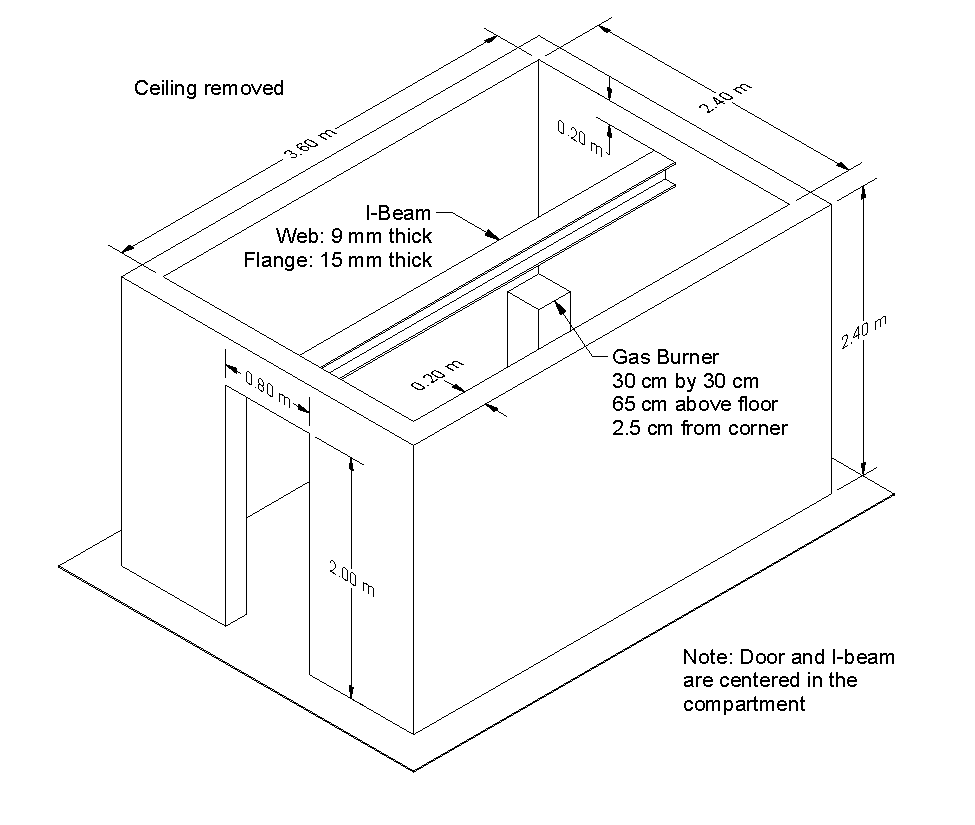
\includegraphics[width=\textwidth]{FIGURES/SP_AST/SP_AST_Compartment_Drawing}
\caption[Geometry of the  SP/AST compartment for Test 2]{Geometry of the  SP/AST compartment for Test 2.}
\label{Room_Drawing}
\end{figure}

A second series of experiments involving plate thermometers was carried out in 2011~\cite{Sjostrom:AST}. A 6~m long, 20~cm diameter vertical steel column was positioned in the center of 1.1~m and 1.9~m diesel fuel and 1.1~m heptane pool fires. Gas, plate thermometer, and surface temperatures were measured at heights of 1~m, 2~m, 3~m, 4~m, and 5~m above the pool surface. These experiments are notable because the column is partially engulfed in flames.

A third series of experiments involving plate thermometers was conducted in 2015~\cite{Sjostrom:SP2016}. A simple compartment with a single door was constructed and instrumented primarily with plate thermometers. The compartment was 2.7~m long, 1.8~m wide, and 1.8~m tall, with a 0.6~m by 1.5~m door centered on one of the short walls. The PTs were affixed to the walls. The 12 experiments were conducted with four different wall linings. In Series~A, the compartment was lined with a 10~cm thick light concrete block. In Series~B, the compartment was lined with a 5~cm thick layer of insulation backed by a 3~mm thick plate of steel. In Series~C, the compartment was lined with an uninsulated 3~mm thick steel plate. In Series~D, the compartment was lined with a 3~mm thick steel plate backed by a 5~cm thick layer of insulation (the opposite of Series~B). The fires were fueled by a 0.3~m by 0.3~m propane burner located in the center of the room except for Test~A3, where it was centered on the back wall. For most of the experiments, the heat release rate was 1000~kW, except for A2 and C1, which were 500~kW, and A4 and C3, which employed linear ramp-ups to 1250~kW.


\section{SP Wood Crib Experiments}
\label{SP_Wood_Cribs_Description}

Hansen and Ingason burned piles of reduced-scale wood pallets in a reduced-scale wind tunnel to develop a simple model that predicts the heat release rate of multiple objects separated by varying distances~\cite{Hansen:2010,Hansen:FSJ2012}. The tunnel was 10~m long with a rectangular cross section 0.6~m wide by 0.4~m tall. Four piles of 1:4 scale pallets were placed at various positions in the tunnel. Each pile of 5 pallets was 0.3~m long, 0.2~m wide and 0.18~m tall. The fire was ignited on the windward side of the upwind pile with a 3~cm by 3~cm by 2.4~cm block of fiberboard soaked in 9~mL of heptane. The HRR was measured, along with temperature, heat flux, and oxygen concentration at various locations.

\subsubsection{Modeling Notes}

The piles of pallets are modeled as an array of Lagrangian particles in lieu of solid obstructions so that a relatively coarse grid of 4~cm can be used. The simulations have previously been performed with partially resolved obstructions~\cite{Janardhan:FT2019}, but such simulations cannot be performed on relatively coarse grids.

The modeling strategy is very similar to that used for vegetation in wildfire simulations. The wood planks are characterized as a homogenous collection of flat disks with a surface area to volume ratio $\sigma=460$~m$^{-1}$ and a packing ratio $\beta=0.42$. The packing ratio is the bulk crib mass per unit volume divided by the density of the wood, $m'''/\rho_{\rm wood}$. The average mass of a pile of pallets is 1.7~kg.

The radiation absorption coefficient is taken as $\kappa=C_{\rm s} \sigma \beta$, where the shape factor, or ratio of plate surface area to projected area, is $C_{\rm s}=0.25$. The absorption coefficient, $\kappa$, also appears in the formula for wind drag, where the pressure drop, $\Delta p$, over a distance, $L$, is given by $\Delta p / L = 0.5 \rho C_{\rm d} \kappa u^2$. The drag coefficient, $C_{\rm d}=2.8$, was measured by Falkenstein-Smith~et~al.~\cite{Falkenstein-Smith:2018} in a study of vegetation. Its application to wood cribs has not been validated.

The wood is assumed to pyrolyze, forming C$_{3.4}$H$_{6.2}$O$_{2.5}$~\cite{Ritchie:1}, according to the following reaction scheme:
\begin{eqnarray}
 {\rm Wet\ Wood} & \rightarrow & \frac{M}{1+M} \, {\rm H_2O} + \frac{1}{1+M} \, {\rm Dry\ Wood} \\[.1in]
 {\rm Dry\ Wood} & \rightarrow & \chi_{\rm char} \, {\rm Char} + (1-\chi_{\rm char}) \, {\rm Fuel\ Gas} \\[.1in]
 {\rm Char} + \nu_{\rm O_2, char} \, {\rm O_2} & \rightarrow & (1+ \nu_{\rm O_2,char} - \chi_{\rm ash}) \, {\rm CO_2} + \chi_{\rm ash} \, {\rm Ash}
\end{eqnarray}
The reaction rates are given by:
\begin{eqnarray}
  r_{\rm H_2O} &=& \left( \frac{\rho_{\rm s,H_2O}}{\rho_{\rm s,0}} \right)        \, A_{\rm H_2O} \, T^{-\frac{1}{2}} \exp \left(  -\frac{E_{\rm H_2O}}{R \, T} \right)  \\[.1in]
  r_{\rm wood} &=& \left( \frac{\rho_{\rm s,wood}}{\rho_{\rm s,0}} \right)^{1.69} \, A_{\rm wood} \,                  \exp \left(  -\frac{E_{\rm wood}}{R \, T} \right)   \\[.1in]
  r_{\rm char} &=& \left( \frac{\rho_{\rm s,char}}{\rho_{\rm s,0}} \right)^0      \, A_{\rm char} \,                  \exp \left(  -\frac{E_{\rm char}}{R \, T} \right) \,
  \frac{ \rho \, Y_{\rm O_2} \, \sigma \, \left( 1+\beta_{\rm char}\sqrt{\RE} \right) }{\nu_{\rm O_2,char} \, \rho_{\rm s,0} }
\end{eqnarray}
The equation governing the temperature of the solid is
\be
\rho_{\rm s} \, c \, \frac{\partial T}{\partial t} = -\rho_{\rm s,0} \left( \Delta{h_{\rm H_2O}}\ r_{\rm H_2O} + \Delta {h_{\rm wood}}\ r_{\rm wood} +  \Delta{h_{\rm char}}\ r_{\rm char} \right) + \nabla \cdot{\mathbf{\dot{q}}}''_{\rm c}  +  \nabla \cdot{\mathbf{\dot{q}}}''_{\rm r}
\ee
The parameters for the pyrolysis model are listed in Table~\ref{Pine_Properties}.

\begin{table}[p]
\caption[Parameters for SP Wood Cribs simulations]{Parameters for SP Wood Cribs simulations.}
\begin{center}
\begin{tabular}{|l|c|c|l|}
\hline
Property                &      Units    &      Value                         & Reference                      \\ \hline \hline
$M$                     &               & 0.016                              & \cite{Hansen:2010}             \\ \hline
$\rho_{\rm H_2O}$       &     kg/m$^3$  & 1000                               & \cite{Porterie:2000PhysFluids} \\ \hline
$c_{\rm H_2O}$          &    kJ/kg/K    & 4.184                              & \cite{Porterie:2000PhysFluids} \\ \hline
$k_{\rm H_2O}$          &      W/m/K    & 0.62                               & \cite{Porterie:2000PhysFluids} \\ \hline
$A_{\rm H_2O}$          & $\sqrt{K}$/s  & 600000                             & \cite{Porterie:2000PhysFluids} \\ \hline
$E_{\rm H_2O}$          & J/mol         & 48200                              & \cite{Porterie:2000PhysFluids} \\ \hline
$\Delta h_{\rm H_2O}$   & kJ/kg         & 2259                               & \cite{Porterie:2000PhysFluids} \\ \hline \hline
$\rho_{\rm wood}$       &     kg/m$^3$  & 370                                &                                \\ \hline
$c_{\rm wood}$          &    kJ/kg/K    & $0.90+0.00235(T-20)$               &                                \\ \hline
$k_{\rm wood}$          &      W/m/K    & $0.10+0.00035(T-20)$               &                                \\ \hline
$\epsilon_{\rm wood}$   &               & 0.95                               & \cite{Ritchie:1}               \\ \hline
$A_{\rm wood}$          & s$^{-1}$      & 141300                             &                                \\ \hline
$E_{\rm wood}$          & J/mol         & 90730                              &                                \\ \hline
$\Delta h_{\rm wood}$   & kJ/kg         & 250                                &                                \\ \hline \hline
$\rho_{\rm char}$       &     kg/m$^3$  & 135                                &                                \\ \hline
$c_{\rm char}$          &    kJ/kg/K    & $0.80+0.00615(T-20)$               &                                \\ \hline
$k_{\rm char}$          &      W/m/K    & $0.11+0.000308(T-20)$              &                                \\ \hline
$\epsilon_{\rm char}$   &               & 1.0                                & Assumption                     \\ \hline
$A_{\rm char}$          & s$^{-1}$      & 430                                & \cite{Porterie:2000PhysFluids} \\ \hline
$E_{\rm char}$          & J/mol         & 74800                              & \cite{Porterie:2000PhysFluids} \\ \hline
$\chi_{\rm char}$       & g/g           & 0.20                               & Assumption                     \\ \hline
$\beta_{\rm char}$      &               & 0.20                               & \cite{Porterie:2006}           \\ \hline
$\nu_{\rm O_2, char}$   & g/g           & 1.65                               & \cite{Porterie:2006}           \\ \hline
$\Delta h_{\rm char}$   & kJ/kg         & -32800                             & \cite{SFPE}                    \\ \hline \hline
$\chi_{\rm ash}$        & g/g           & 0.02                               & Assumption                     \\ \hline
$\rho_{\rm ash}$        &     kg/m$^3$  & 67                                 & Assumption                     \\ \hline
$c_{\rm ash}$           &    kJ/kg/K    & 2.0                                & Assumption                     \\ \hline
$k_{\rm char}$          &      W/m/K    & 0.1                                & Assumption                     \\ \hline \hline
$\Delta h$              &      kJ/kg    & 18100                              & \cite{Hansen:2010}             \\ \hline
\end{tabular}
\end{center}
\label{Pine_Properties}
\end{table}


\section{Steckler Compartment Experiments}
\label{Steckler_Description}

Steckler, Quintiere and Rinkinen performed a set of 55 compartment fire tests at NBS in 1979. The compartment was 2.8~m by 2.8~m by 2.13~m high\footnote{The test report gives the height of the compartment as 2.18~m. This is a misprint. The compartment was 2.13~m high.}, with a single door of various widths, or alternatively a single window with various heights. A 30~cm diameter methane burner was used to generate fires with heat release rates of 31.6~kW, 62.9~kW, 105.3~kW and 158~kW. Vertical profiles of velocity and temperature were measured in the doorway, along with a single vertical profile of temperature within the compartment. A full description and results are reported in Reference~\cite{Steckler:NBSIR_82-2520}. The basic test matrix is listed in Table~\ref{Steckler_Table}. Note that the test report does not include a detailed description of the compartment. However, an internal report\footnote{ {\em Technical Research Report, Fire Induced Flows Through Room Openings - Flow Coefficients}, Project 203005-003, Armstrong Cork Company, Lancaster, Pennsylvania, May, 1981.} by the test sponsor, Armstrong Cork Company, reports that the compartment floor was composed of 19~mm calcium silicate board on top of 12.7~mm plywood on wood joists. The walls and ceiling consisted of 12.7~mm ceramic fiber insulation board over 0.66~mm aluminum sheet attached to wood studs. A diagram of the compartment is displayed in Fig.~\ref{Steckler_ Drawing}.

\begin{table}[h!]
\caption[Summary of Steckler compartment experiments]{Summary of Steckler compartment experiments.}
\begin{center}
\begin{tabular}{|c|c|c|c|c||c|c|c|c|c|}
\hline
        & Door      & Door          &  HRR       & Burner       &       & Door      & Door        &  HRR         & Burner        \\
Test    & Width     & Height        & $\dot{Q}$  & Location     & Test  & Width     & Height      & $\dot{Q}$    & Location      \\
        & (m)       & (m)           & (kW)       &              &       & (m)       &  (m)        & (kW)         &                \\ \hline \hline
10      & 0.24      & 1.83          &  62.9      & Center       & 224   & 0.74      & 0.92        &  62.9         & Back Corner         \\ \hline
11      & 0.36      & 1.83          &  62.9      & Center       & 324   & 0.74      & 0.92        &  62.9         & Back Corner         \\ \hline
12      & 0.49      & 1.83          &  62.9      & Center       & 220   & 0.74      & 1.83        &  31.6         & Back Corner         \\ \hline
612     & 0.49      & 1.83          &  62.9      & Center       & 221   & 0.74      & 1.83        &  105.3        & Back Corner         \\ \hline
13      & 0.62      & 1.83          &  62.9      & Center       & 514   & 0.24      & 1.83        &  62.9         & Back Wall           \\ \hline
14      & 0.74      & 1.83          &  62.9      & Center       & 544   & 0.36      & 1.83        &  62.9         & Back Wall           \\ \hline
18      & 0.74      & 1.83          &  62.9      & Center       & 512   & 0.49      & 1.83        &  62.9         & Back Wall           \\ \hline
710     & 0.74      & 1.83          &  62.9      & Center       & 542   & 0.62      & 1.83        &  62.9         & Back Wall           \\ \hline
810     & 0.74      & 1.83          &  62.9      & Center       & 610   & 0.74      & 1.83        &  62.9         & Back Wall           \\ \hline
16      & 0.86      & 1.83          &  62.9      & Center       & 510   & 0.74      & 1.83        &  62.9         & Back Wall           \\ \hline
17      & 0.99      & 1.83          &  62.9      & Center       & 540   & 0.86      & 1.83        &  62.9         & Back Wall           \\ \hline
22      & 0.74      & 1.38          &  62.9      & Center       & 517   & 0.99      & 1.83        &  62.9         & Back Wall           \\ \hline
23      & 0.74      & 0.92          &  62.9      & Center       & 622   & 0.74      & 1.38        &  62.9         & Back Wall           \\ \hline
30      & 0.74      & 0.92          &  62.9      & Center       & 522   & 0.74      & 1.38        &  62.9         & Back Wall           \\ \hline
41      & 0.74      & 0.46          &  62.9      & Center       & 524   & 0.74      & 0.92        &  62.9         & Back Wall           \\ \hline
19      & 0.74      & 1.83          &  31.6      & Center       & 541   & 0.74      & 0.46        &  62.9         & Back Wall           \\ \hline
20      & 0.74      & 1.83          &  105.3     & Center       & 520   & 0.74      & 1.83        &  31.6         & Back Wall           \\ \hline
21      & 0.74      & 1.83          &  158.0     & Center       & 521   & 0.74      & 1.83        &  105.3        & Back Wall           \\ \hline
114     & 0.24      & 1.83          &  62.9      & Back Corner  & 513   & 0.74      & 1.83        &  158.0        & Back Wall           \\ \hline
144     & 0.36      & 1.83          &  62.9      & Back Corner  & 160   & 0.74      & 1.83        &  62.9         & Center$^*$          \\ \hline
212     & 0.49      & 1.83          &  62.9      & Back Corner  & 163   & 0.74      & 1.83        &  62.9         & Back Corner$^*$     \\ \hline
242     & 0.62      & 1.83          &  62.9      & Back Corner  & 164   & 0.74      & 1.83        &  62.9         & Back Wall$^*$       \\ \hline
410     & 0.74      & 1.83          &  62.9      & Back Corner  & 165   & 0.74      & 1.83        &  62.9         & Left Wall$^*$       \\ \hline
210     & 0.74      & 1.83          &  62.9      & Back Corner  & 162   & 0.74      & 1.83        &  62.9         & Right Wall$^*$      \\ \hline
310     & 0.74      & 1.83          &  62.9      & Back Corner  & 167   & 0.74      & 1.83        &  62.9         & Front Center$^*$    \\ \hline
240     & 0.86      & 1.83          &  62.9      & Back Corner  & 161   & 0.74      & 1.83        &  62.9         & Doorway$^*$         \\ \hline
116     & 0.99      & 1.83          &  62.9      & Back Corner  & 166   & 0.74      & 1.83        &  62.9         & Front Corner$^*$    \\ \hline
122     & 0.74      & 1.38          &  62.9      & Back Corner  &  \multicolumn{5}{r|}{$^*$ Raised burner}                   \\ \hline
\end{tabular}
\end{center}
\label{Steckler_Table}
\end{table}


\begin{figure}[!ht]
\includegraphics[width=\textwidth]{FIGURES/Steckler_Compartment/Steckler_Room_Drawing}
\caption[Geometry of the Steckler Compartment Experiments]{Geometry of the Steckler Compartment Experiments.}
\label{Steckler_ Drawing}
\end{figure}


\FloatBarrier


\section{SWJTU Tunnel Experiments}
\label{SSJTU_Tunnel_Description}

Fires fueled by methanol and propane ranging from 5.6~kW to 16.8~kW were conducted in a 1:20 reduced-scale tunnel at Southwest Jiaotong University, Chengdu, China~\cite{Wang:TUST2019}. The tunnel was 0.45~m wide, 0.23~m high and 20.8~m long. The burner was located at the center of the tunnel and both ends were open. Temperatures and gas concentrations (i.e., O$_2$, CO and CO$_2$) were measured. The results showed that both methanol and propane fires self-extinguished in the 20.8~m long tunnel within approximately 10~min, except for the 5.6~kW methanol fire. The larger the heat release rate, the faster the self-extinction of the fire. The oxygen concentrations in the 20.8~m long tunnel decreased to approximately 12~\% except for the 5.6~kW methanol fire, which remained well above the limiting oxygen concentration.  Self-extinction was not observed for fires of the same heat release rates in a 10~m long tunnel of the same cross section. The oxygen concentrations in the 10~m long tunnel decreased to approximately 17~\%.  In the long tunnel with large fire sizes, the smoke layer descended to the floor, inhibiting the supply of fresh air reaching the fire.




\section{UL/NIST Vent Experiments}
\label{UL_NIST_Vents_Description}

In 2012, the Fire Fighting Technology Group at NIST conducted experiments at Underwriters Laboratories (UL) in Northbrook, Illinois, to assess the change in compartment temperature due to the opening of one or two 1.2~m square ceiling vents~\cite{Opert:Masters}. Four experiments were conducted using a natural gas burner in a 6.1~m by 4.3~m by 2.4~m compartment with a single door opening. The fires ranged in size from 500~kW to 2~MW, and the vents were opened and closed such that during the four experiments there were 31 discrete time intervals in which model predictions could be compared to quasi-steady conditions. The compartment contained two vertical arrays of thermocouples, and the door and vents were instrumented with thermocouples and bi-directional velocity probes. Only the thermocouple data has been used in the validation study. A diagram of the compartment is displayed in Figure~\ref{UL_NIST_Drawing}. The major test parameters are listed in Table~\ref{UL_NIST_Table}.

\begin{figure}[ht]
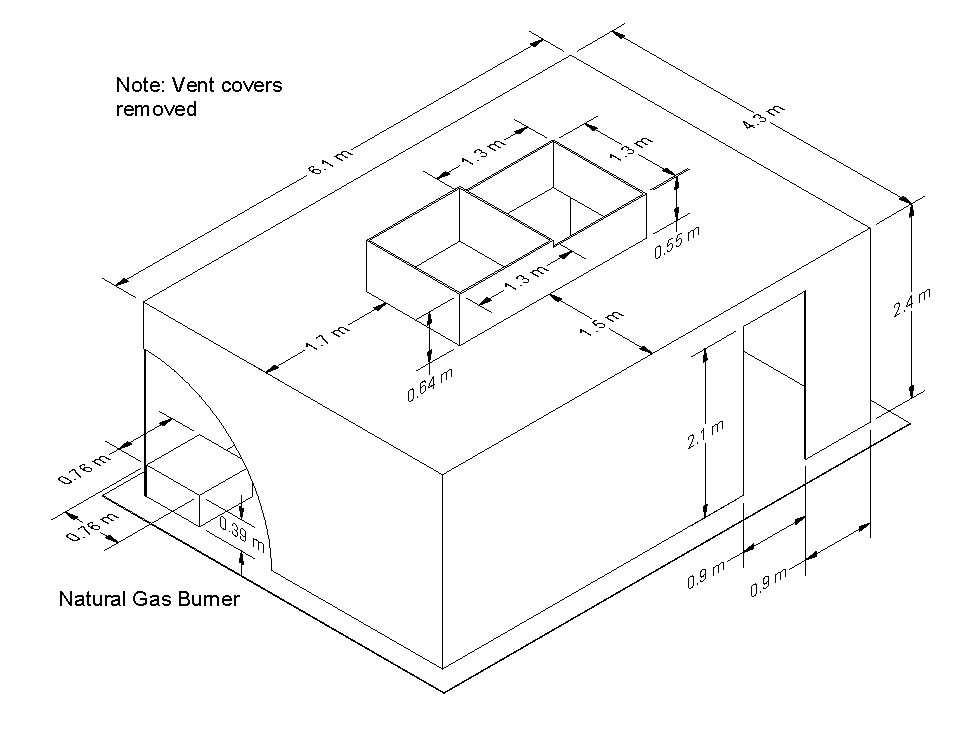
\includegraphics[width=\textwidth]{FIGURES/UL_NIST_Vents/UL_NIST_Vents_Drawing}
\caption{Geometry of the UL/NIST Experiments.}
\label{UL_NIST_Drawing}
\end{figure}


\begin{table}[h!]
\caption[Summary of UL/NIST Vent experiments]{Summary of UL/NIST Vent experiments. Note that the 31 ``experiments'' are actually discrete time intervals during the course of four separate fires.}
\begin{center}
\begin{tabular}{|c|c|c|c||c|c|c|c|}
\hline
Exp.    & End Time  & HRR           &  No. of   & Exp.    & End Time  & HRR           &  No. of           \\
No.     & (s)       & (kW)          & Vents     & No.     & (s)       & (kW)          & Vents             \\ \hline \hline
\multicolumn{4}{|c||}{Fire 1}                   & \multicolumn{4}{|c|}{Fire 3}                            \\ \hline
1       & 1215      & 430           & 0         & 14      & 453       & 476           & 0                 \\ \hline
2       & 1840      & 430           & 1         & 15      & 816       & 476           & 1                 \\ \hline
3       & 2168      & 430           & 2         & 16      & 1153      & 476           & 2                 \\ \hline
4       & 2474      & 430           & 0         & 17      & 1640      & 1002          & 0                 \\ \hline
5       & 2955      & 1011          & 0         & 18      & 1936      & 1002          & 1                 \\ \hline
6       & 3170      & 1011          & 1         & 19      & 2233      & 1002          & 2                 \\ \hline
7       & 3604      & 1011          & 2         & \multicolumn{4}{|c|}{Fire 4}                            \\ \hline
8       & 3840      & 1011          & 0         & 20      & 519       & 1011          & 0                 \\ \hline
9       & 4153      & 2188          & 0         & 21      & 967       & 1011          & 1                 \\ \hline
10      & 4284      & 2188          & 1         & 22      & 1325      & 1011          & 2                 \\ \hline
\multicolumn{4}{|c||}{Fire 2}                   & 23      & 1559      & 470           & 2                 \\ \hline
11      & 565       & 2144          & 0         & 24      & 1653      & 470           & 1                 \\ \hline
12      & 833       & 2144          & 1         & 25      & 2013      & 470           & 0                 \\ \hline
13      & 931       & 2144          & 2         & 26      & 2411      & 470           & 1                 \\ \hline
\multicolumn{4}{|r||}{}                         & 27      & 2910      & 470           & 2                 \\ \cline{5-8}
\multicolumn{4}{|r||}{}                         & 28      & 3399      & 2188          & 2                 \\ \cline{5-8}
\multicolumn{4}{|r||}{}                         & 29      & 3586      & 2188          & 0                 \\ \cline{5-8}
\multicolumn{4}{|r||}{}                         & 30      & 3803      & 2188          & 1                 \\ \cline{5-8}
\multicolumn{4}{|r||}{}                         & 31      & 4035      & 2188          & 2                 \\ \hline
\end{tabular}
\end{center}
\label{UL_NIST_Table}
\end{table}


\FloatBarrier

\section{UL/NFPRF Sprinkler, Vent, and Draft Curtain Study}
\label{UL_NFPRF_Description}

In 1997, thirty-four heptane spray burner and five racked commodity experiments were conducted at the Large Scale Fire Test Facility at Underwriters Laboratories (UL) in Northbrook, Illinois~\cite{Sheppard:1,McGrattan:5}. The spray burner experiments were divided into two test series. Series I consisted of 22 4.4~MW experiments. Series~II consisted of 12 10~MW experiments. The objective of the spray burner experiments was to characterize the temperature and flow field for fire scenarios with a controlled heat release rate in the presence of sprinklers, draft curtains, and smoke \& heat vents.

The Large Scale Fire Test Facility at UL contains a 37~m by 37~m (120~ft by 120~ft) main fire test cell, equipped with a 30.5~m by 30.5~m (100~ft by 100~ft) adjustable height ceiling. The UL/NFPRF test results (Series I) are summarized in Table~\ref{ULmatrix}. The UL/NFPRF test results (Series II) are summarized in Table~\ref{ULburnermatrixII}. The layout of the experiments is shown in Figs.~\ref{layout}, \ref{burnerlayoutA}, and \ref{layout3}.

\begin{table}[h!]
\begin{center}
\begin{tabular}{|c||c|c|c|c|c|c|}
\hline
\multicolumn{7}{|c|}{\bf Heptane Spray Burner Test Series I}  \\ \hline \hline
Test & Burner & Vent                    & First         & Total      & Draft    & Heat Release Rate \\
No.  & Pos.   & Operation               & Actuation (s) & Actuations & Curtains & MW @ s \\
\hline \hline
I-1   & B  & Closed                     & 65            & 11        & Yes  & 4.4 @ 50  \\ \hline
I-2   & B  & Manual (0:40)              & 66            & 12        & Yes  & 4.4 @ 50  \\ \hline
I-3   & B  & Manual (1:30)              & 64            & 12        & Yes  & 4.4 @ 50  \\ \hline
I-4   & C  & Closed                     & 60            & 10        & Yes  & 4.4 @ 50  \\ \hline
I-5   & C  & Manual (0:40)              & 72            & 9         & Yes  & 4.4 @ 50  \\ \hline
I-6   & C  & Manual (1:30)              & 62            & 8         & Yes  & 4.4 @ 50  \\ \hline
I-7   & C  & 74$^\circ$C link (DNO)     & 70            & 10        & Yes  & 4.4 @ 50  \\ \hline
I-8   & B  & 74$^\circ$C link (9:26)    & 60            & 11        & Yes  & 4.4 @ 50  \\ \hline
I-9   & D  & 74$^\circ$C link (DNO)     & 70            & 12        & Yes  & 4.4 @ 50  \\ \hline
I-10  & D  & Manual (0:40)              & 72            & 13        & Yes  & 4.4 @ 50  \\ \hline
I-11  & D  & 74$^\circ$C link (4:48)    & N/A           & N/A       & Yes  & 4.4 @ 50  \\ \hline
I-12  & A  & Closed                     & 68            & 14        & Yes  & 4.4 @ 50  \\ \hline
I-13  & A  & 74$^\circ$C link (1:04)    & 69            & 5         & Yes  & 6.0 @ 60  \\ \hline
I-14  & A  & Manual (0:40)              & 74            & 7         & Yes  & 5.8 @ 60  \\ \hline
I-15  & A  & Manual (1:30)              & 64            & 5         & Yes  & 5.8 @ 60  \\ \hline
I-16  & A  & 74$^\circ$C link (1:46)    & 106           & 4         & Yes  & 5.0 @ 110 \\ \hline \hline
I-17  & B  & 100$^\circ$C link (DNO)    & 58            & 4         & No   & 4.6 @ 50 \\ \hline
I-18  & C  & 100$^\circ$C link (DNO)    & 58            & 4         & No   & 3.7 @ 50 \\ \hline
I-19  & A  & 100$^\circ$C link (10:00)  & 56            & 10        & No   & 4.6 @ 50 \\ \hline
I-20  & A  & 74$^\circ$C link (1:20)    & 54            & 4         & No   & 4.2 @ 50 \\ \hline
I-21  & C  & 74$^\circ$C link (7:00)    & 58            & 10        & No   & 4.6 @ 50 \\ \hline
I-22  & D  & 100$^\circ$C link (DNO)    & 60            & 6         & No   & 4.6 @ 50 \\ \hline
\end{tabular}
\end{center}
\caption[Results of the UL/NFPRF heptane spray experiments, Series~I]
{Results of Series~I of the UL/NFPRF heptane spray experiments. Note that DNO means ``Did Not Open''. Also note, the fires grew at a rate proportional to the square of the time until a certain flow rate of fuel was achieved at which time the flow rate was held steady. Thus, the ``Heat Release Rate'' was the size of the fire at the time when the fuel supply was leveled off.}
\label{ULmatrix}
\end{table}

\begin{figure}[p]
\begin{center}
\setlength{\unitlength}{.05416667in}
\begin{picture}(120,120)

\linethickness{1.mm} \put(0,0){\framebox(120,120)[tc]{North Wall}} \linethickness{.5mm} \put(10,10){\framebox(100,100)[tc]{Adjustable Height
Ceiling}}

\thinlines \put(117,67){\vector(0,-1){67}} \put(117,73){\vector(0, 1){47}} \put(117,70){\makebox(0,0){$120'$}} \put(113,57){\vector(0,-1){47}}
\put(111,110){\line(1,0){4.}} \put(111, 10){\line(1,0){4.}} \put(113,63){\vector(0, 1){47}} \put(113,60){\makebox(0,0){$100'$}}
\put(30.9,12.83){\dashbox{1}(67.1,71.17)[tc]{Draft Curtains}} \put(27.9,40){\vector(0,-1){27.17}} \put(27.9,46){\vector(0, 1){38.0}}
\put(25.9,84.){\line(1,0){4.}} \put(25.9,12.83){\line(1,0){4.}} \put(27.9,43){\makebox(0,0){$71'2''$}} \put(64.0,87.){\vector(-1,0){33.1}}
\put(72.0,87.){\vector( 1,0){26.0}} \put(30.9,85.){\line(0,1){4.}} \put(98.0,85.){\line(0,1){4.}} \put(68.0,87.){\makebox(0,0){$67'1''$}}

\put(16.0,87.){\vector(-1,0){6.}} \put(24.0,87.){\vector( 1,0){6.92}} \put(20.0,87.){\makebox(0,0){$20'11''$}} \put(101.,87.){\vector(-1,0){3.}}
\put(107.,87.){\vector( 1,0){3.}} \put(104.,87.){\makebox(0,0){$12'$}}

\put(27.9,100){\vector(0,1){10.}} \put(27.9,94){\vector(0,-1){10.}} \put(27.9,97){\makebox(0,0){$26'$}}

\put(27.9,8){\vector(0,1){2.}} \put(27.9,8){\line(1,0){3.}} \put(30.9,8){\makebox(0,0)[l]{$2'10''$}}

\put(55.08,14.83){\line(-1,0){2.}} \put(54.08,16.83){\vector(0,-1){2.}} \put(54.08,7.83){\vector(0,1){5.}} \put(54.08,7.83){\line(1,0){3.}}
\put(57.08,7.83){\makebox(0,0)[l]{$2'$}}

\put(85.08,24.83){\line(0,-1){2.}} \put(95.08,24.83){\line(0,-1){2.}} \put(93.08,23.83){\vector(1,0){2.}} \put(87.08,23.83){\vector(-1,0){2.}}
\put(103.00,23.83){\vector(-1,0){5.}} \put(103.00,23.83){\line(0,-1){3.}} \put(103.00,20.83){\makebox(0,0)[ct]{$2'11''$}}
\put(90.08,23.83){\makebox(0,0)[c]{$10'$}}

\thicklines \put(78.08,55.83){\framebox(4,8){ }}

\put(78.58,58.33){\framebox(3,3)[c]{A}} \put(78.58,68.33){\framebox(3,3)[c]{B}} \put(88.58,58.33){\framebox(3,3)[c]{C}}
\put(58.58,38.33){\framebox(3,3)[c]{D}}

\thinlines

\multiput(35.08,14.83)(0,10){7}{\circle*{.8}} \multiput(45.08,14.83)(0,10){7}{\circle*{.8}} \multiput(55.08,14.83)(0,10){7}{\circle*{.8}}
\multiput(65.08,14.83)(0,10){7}{\circle*{.8}} \multiput(75.08,14.83)(0,10){7}{\circle*{.8}} \multiput(85.08,14.83)(0,10){7}{\circle*{.8}}
\multiput(95.08,14.83)(0,10){7}{\circle*{.8}} \tiny \put(35.48,15.23){98} \put(45.48,15.23){91} \put(55.48,15.23){84} \put(65.48,15.23){81}
\put(75.48,15.23){78} \put(85.48,15.23){75} \put(95.48,15.23){72} \put(35.48,25.23){99} \put(45.48,25.23){92} \put(55.48,25.23){85}
\put(65.48,25.23){82} \put(75.48,25.23){79} \put(85.48,25.23){76} \put(95.48,25.23){73} \put(35.48,35.23){100} \put(45.48,35.23){93}
\put(55.48,35.23){86} \put(65.48,35.23){83} \put(75.48,35.23){80} \put(85.48,35.23){77} \put(95.48,35.23){74} \put(35.48,45.23){101}
\put(45.48,45.23){94} \put(55.48,45.23){87} \put(65.48,45.23){62} \put(75.48,45.23){58} \put(85.48,45.23){54} \put(95.48,45.23){50}
\put(35.48,55.23){102} \put(45.48,55.23){95} \put(55.48,55.23){88} \put(65.48,55.23){63} \put(75.48,55.23){59} \put(85.48,55.23){55}
\put(95.48,55.23){51} \put(35.48,65.23){103} \put(45.48,65.23){96} \put(55.48,65.23){89} \put(65.48,65.23){64} \put(75.48,65.23){60}
\put(85.48,65.23){56} \put(95.48,65.23){52} \put(35.48,75.23){104} \put(45.48,75.23){97} \put(55.48,75.23){90} \put(65.48,75.23){65}
\put(75.48,75.23){61} \put(85.48,75.23){57} \put(95.48,75.23){53} \put(70.08,49.83){\makebox(0,0)[c]{68}} \put(70.08,59.83){\makebox(0,0)[c]{69}}
\put(70.08,69.83){\makebox(0,0)[c]{70}} \put(80.08,49.83){\makebox(0,0)[c]{67}} \put(90.08,49.83){\makebox(0,0)[c]{66}}
\put(90.08,69.83){\makebox(0,0)[c]{71}}

\multiput(80.08,56.83)(0,1){7}{\circle*{.2}} \put(80.58,62.83){\line(1,0){22.5}} \put(104.,62.83){\makebox(0,0)[l]{43}}
\put(104.,61.33){\makebox(0,0)[l]{44}} \put(104.,59.83){\makebox(0,0)[l]{45}} \put(104.,58.33){\makebox(0,0)[l]{46}}
\put(104.,56.83){\makebox(0,0)[l]{47}} \put(104.,55.33){\makebox(0,0)[l]{48}} \put(104.,53.83){\makebox(0,0)[l]{49}}

\normalsize

\end{picture}
\end{center}
\caption[Plan view of the UL/NFPRF heptane spray experiments, Series~I] {Plan view of the UL/NFPRF heptane spray experiments, Series~I. The sprinklers are indicated by the solid circles and are spaced exactly 10~ft apart. The number beside each sprinkler location indicates the channel number of the nearest thermocouple. The vent dimensions are 4~ft by 8~ft. The boxed letters A, B, C and D indicate burner positions. Corresponding to each burner position is a vertical array of thermocouples. Thermocouples 1--9 hang 7, 22, 36, 50, 64, 78, 92, 106 and 120~in from the ceiling, respectively, above Position A. Thermocouples 10 and 11 are positioned above and below the ceiling tile directly above Position B, followed by 12--20 that hang at the same levels below the ceiling as 1--9. The same pattern is followed at Positions C and D, with thermocouples 21--31 at C and 32--42 at D.}
\label{layout}
\end{figure}




\begin{table}[ht!]
\begin{center}
\begin{tabular}{|c||c|c|c|c|c|c|c|}
\hline
\multicolumn{8}{|c|}{\bf Heptane Spray Burner Test Series II (10 MW Fires)}\\ \hline \hline
Test & Burner   & Vent      & Sprinklers & First      & Last      & \multicolumn{2}{|c|}{Avg.~Peak Temp.} \\ \cline{7-8}
No.  & Position & Operation & Opened     & Activation & Activation & $^\circ$C & $^\circ$F   \\
\hline \hline
II-1  & D  & 74$^\circ$C link (DNO)  & 27 & 1:15 & 6:13 & 129.4 &264.9 \\ \hline
II-2  & D  & All Open at Start       & 28 & 1:05 & 5:53 & 128.8 &263.8 \\ \hline
II-3  & A  & 74$^\circ$C link (1:15) & 12 & 1:08 & 4:00 & 101.8 &215.2 \\ \hline
II-4  & B  & 74$^\circ$C link (1:48) & 16 & 1:03 & 5:54 & 108.8 &227.8 \\ \hline
II-5  & D  & 74$^\circ$C link (DNO)  & 28 & 1:10 & 7:07 & 130.0 &266.0 \\ \hline
II-6  & D  & All Open at Start       & 27 & 1:10 & 5:21 & 127.5 &261.5 \\ \hline
II-7  & A  & Closed                  & 18 & 1:09 & 4:11 & 117.2 &243.0 \\ \hline
II-8  & B  & 74$^\circ$C link (1:12) & 13 & 1:10 & 3:34 & 107.7 &225.9 \\ \hline
II-9  & E  & 74$^\circ$C link (DNO)  & 23 & 1:07 & 3:28 & 115.8 &240.4 \\ \hline
II-10 & F  & 74$^\circ$C link (3:20) & 19 & 1:14 & 3:01 & 108.4 &227.1 \\ \hline
II-11 & C  & 74$^\circ$C link (DNO)  & 23 & 1:02 & 3:56 & 123.4 &254.1 \\ \hline
II-12 & C  & All Open at Start       & 23 & 0:58 & 4:55 & 119.0 &246.2 \\ \hline
\end{tabular}
\end{center}
\caption[Results of the UL/NFPRF heptane spray experiments, Series~II]
{Results of the UL/NFPRF heptane spray experiments, Series II. Note that all fires were ramped up to 10~MW in 75~s following a $t$-squared curve.}
\label{ULburnermatrixII}
\end{table}


\begin{figure}[p]
\begin{center}
\setlength{\unitlength}{.054166in}
\begin{picture}(120,120)

\linethickness{1mm}
\put(0,0){\framebox(120,120)[tc]{ }}
\put(60,118){\makebox(0,0){North Wall}}
\put(60,  2){\makebox(0,0){South Wall}}

\linethickness{.5mm}
\put(10,10){\framebox(100,100)[tl]{ }}

\thinlines
\put(117,67){\vector(0,-1){67}}
\put(117,73){\vector(0, 1){47}}
\put(117,70){\makebox(0,0){$120'$}}
\put(113,57){\vector(0,-1){47}}
\put(113,63){\vector(0, 1){47}}
\put(113,60){\makebox(0,0){$100'$}}
\put(10.0,86.0){\dashbox{1}(30.0,24.0)[tl]{ }}
\put(40.,10.5){\dashbox{1}(69.5,75.5)[tl]{              }}

\thicklines
\put(48.,16.){\framebox(4,8){ }}
\put(48.,67.){\framebox(4,8){ }}
\put(28.,67.){\framebox(4,8){ }}
\put(98.,67.){\framebox(4,8){ }}
\put(98.,16.){\framebox(4,8){ }}

\large
\put(68.5,49.5){\dashbox{.5}(3,3)[c]{D}}
\put(48.5,69.5){\dashbox{.5}(3,3)[c]{A}}
\put(48.5,79.5){\dashbox{.5}(3,3)[c]{B}}
\put(58.5,59.5){\dashbox{.5}(3,3)[c]{C}}
\put(38.5,54.5){\dashbox{.5}(3,3)[c]{E}}
\put(38.5,84.5){\dashbox{.5}(3,3)[c]{F}}
\normalsize

\multiput(15,11)(0,10){10}{\circle*{.8}}
\multiput(25,11)(0,10){10}{\circle*{.8}}
\multiput(35,11)(0,10){10}{\circle*{.8}}
\multiput(45,11)(0,10){10}{\circle*{.8}}
\multiput(55,11)(0,10){10}{\circle*{.8}}
\multiput(65,11)(0,10){10}{\circle*{.8}}
\multiput(75,11)(0,10){10}{\circle*{.8}}
\multiput(85,11)(0,10){10}{\circle*{.8}}
\multiput(95,11)(0,10){10}{\circle*{.8}}
\multiput(105,11)(0,10){10}{\circle*{.8}}

\end{picture}
\end{center}
\caption[Plan view of the UL/NFPRF heptane spray experiments, Series~II ]
{Plan view of the UL/NFPRF heptane spray experiments, Series~II. The boxed letters A, B, C, D, E and F indicate burner positions. The sprinklers are indicated by the solid circles and are spaced exactly 10~ft apart. The vents are 4~ft by 8~ft. }
\label{burnerlayoutA}
\end{figure}

\setlength{\unitlength}{.054166in}
\newsavebox{\eightbox}
\savebox{\eightbox}(3.5,3.5){%
\put(0,0){\framebox(3.5,3.5){ }}
\put(1.75,0){\line(0,1){3.5}}
\put(0,1.75){\line(1,0){3.5}}}

\newsavebox{\onebox}
\savebox{\onebox}(3.5,3.5){%
\put(0,0){\framebox(3.5,3.5){ }}}

\thinlines
\newsavebox{\fuel}
\savebox{\fuel}(31.5,30.5){%
\multiput( 0.000, 0.0)(4.000,0){ 2}{\usebox{\onebox}}
\multiput( 8.000, 0.0)(4.000,0){ 4}{\usebox{\eightbox}}
\multiput(24.000, 0.0)(4.000,0){ 2}{\usebox{\onebox}}
\multiput( 0.000,11.5)(4.000,0){8}{\usebox{\eightbox}}
\multiput( 0.000,15.5)(4.000,0){8}{\usebox{\eightbox}}
\multiput( 0.000,27.0)(4.000,0){ 2}{\usebox{\onebox}}
\multiput( 8.000,27.0)(4.000,0){ 4}{\usebox{\eightbox}}
\multiput(24.000,27.0)(4.000,0){ 2}{\usebox{\onebox}}
\put(15.000,13.25){\framebox(.5,.5){ }}
\put(16.000,12.75){\framebox(.5,.5){ }}
\put(16.000,13.25){\framebox(.5,.5){ }}
\put(15.000,12.75){\framebox(.5,.5){ }}
}

\begin{figure}[p]
\begin{center}
\setlength{\unitlength}{.054166in}
\begin{picture}(120,120)

\linethickness{1mm}
\put(0,0){\framebox(120,120)[tc]{ }}
\put(60,118){\makebox(0,0){North Wall}}
\put(60,  2){\makebox(0,0){South Wall}}

\linethickness{.5mm}
\put(10,10){\framebox(100,100)[tl]{ }}

\thinlines
\put(10.0,86.0){\dashbox{1}(30.0,24.0)[tl]{ }}
\put(40.,10.5){\dashbox{1}(69.5,75.5)[tl]{              }}

\thicklines
\put(48.,16.){\framebox(4,8){ }}
\put(48.,67.){\framebox(4,8){ }}
\put(28.,67.){\framebox(4,8){ }}
\put(98.,67.){\framebox(4,8){ }}
\put(98.,16.){\framebox(4,8){ }}

\put(34.25,67.75){\usebox{\fuel}}

\multiput(15,11)(0,10){10}{\circle*{.8}}
\multiput(25,11)(0,10){10}{\circle*{.8}}
\multiput(35,11)(0,10){10}{\circle*{.8}}
\multiput(45,11)(0,10){10}{\circle*{.8}}
\multiput(55,11)(0,10){10}{\circle*{.8}}
\multiput(65,11)(0,10){10}{\circle*{.8}}
\multiput(75,11)(0,10){10}{\circle*{.8}}
\multiput(85,11)(0,10){10}{\circle*{.8}}
\multiput(95,11)(0,10){10}{\circle*{.8}}
\multiput(105,11)(0,10){10}{\circle*{.8}}

\end{picture}
\end{center}
\caption[Plan view of the UL/NFPRF plastic commodity Test P-3]
{Plan view of the UL Large Scale Fire Test Facility with the layout of plastic commodity Test P-3. Tests P-1 and P-2 did not include the draft curtains (dashed lines). The sprinklers (dots) were separated by exactly 10~ft. The racks were located 30~ft south and 20~ft east of the position shown in Tests~P-1, P-4, and P-5. The racks were located 10~ft south of the position shown in Test~P-2. Each pallet load of boxed plastic commodity is represented by a square subdivided into four smaller squares to depict the individual boxes. Pallets containing empty boxes are represented by empty squares. Roof vents are represented by rectangles.}
\label{layout3}
\end{figure}

\begin{description}
\item[Ceiling:] The ceiling was raised to a height of 7.6~m and instrumented with thermocouples and other measurement devices. The ceiling was constructed of 0.6~m by 1.2~m by 1.6~cm UL fire-rated Armstrong Ceramaguard (Item 602B) ceiling tiles. The manufacturer reported the thermal properties of the material to be: specific heat 753 J/(kg$\cdot$K), thermal conductivity 0.0611~W/(m$\cdot$K), and density 313~kg/m$^3$.
\item[Draft Curtains:] Sheet metal, 1.2~mm thick and 1.8~m deep, was suspended from the ceiling for 16 of the 22 Series~I tests, enclosing an area of about 450~m$^2$ and 49 sprinklers. The curtains were in place for all of the Series~II tests.
\item[Sprinklers:] Central ELO-231 (Extra Large Orifice) uprights were used for all the tests. The orifice diameter of this sprinkler is reported by the manufacturer to be nominally 1.6~cm (0.64~in), the reference actuation temperature is reported by the manufacturer to be 74$^\circ$C (165$^\circ$F). The RTI (Response Time Index) and C-factor (Conductivity factor) were reported by UL to be 148~(m$\cdot$s)$^\ha$ and 0.7~(m/s)$^\ha$, respectively~\cite{Sheppard:1}. When installed, the sprinkler deflector was located 8~cm below the ceiling. The thermal element of the sprinkler was located 11~cm below the ceiling. The sprinklers were installed with nominal 3~m by 3~m (exact 10~ft by 10~ft) spacing in a system designed to deliver a constant 0.34~L/(s$\cdot$m$^2$) (0.50 gpm/ft$^2$) discharge density when supplied by a 131~kPa (19~psi) discharge pressure
\item[Vent:] UL-listed double leaf fire vents with steel covers and steel curb were installed in the adjustable height ceiling in the position shown in Figs.~\ref{layout} and \ref{burnerlayoutA}. The vent is designed to open manually or automatically. The vent doors were recessed into the ceiling about 0.3~m (1~ft).
\item[Heptane Spray Burner:] The heptane spray burner consisted of a 1~m by 1~m square of 1.3~cm pipe supported by four cement blocks 0.6~m off the floor. Four atomizing spray nozzles were used to provide a free spray of heptane that was then ignited. For all but one of the Series~I tests, the total heat release rate from the fire was manually ramped up following a ``t-squared'' curve to a steady-state in 75~s (150~s was used in Test I-16). The fire was ramped to 10~MW in 75~s for the Series~II tests. The fire growth curve was followed until a specified fire size was reached or the first sprinkler activated. After either of these events, the fire size was maintained at that level until conditions reached roughly a steady state, i.e., the temperatures recorded near the ceilings remained steady and no more sprinkler activations occurred. The heat release rate from the burner was confirmed by placing it under the large product calorimeter at UL, ramping up the flow of heptane in the same manner as in the tests, and measuring the total and convective heat release rates. It was found that the convective heat release rate was 0.65~$\pm$~0.02 of the total.
\item[Plastic Commodity:] The Factory Mutual Research Corporation (FMRC) standard ``Group A Plastic'' test commodity served as the fuel for the rack storage experiments~\cite{Troup:1}. The cartoned plastic commodity consists of rigid crystalline polystyrene cups packaged in compartmented, single-wall, corrugated paper cartons. Each carton is a cube 0.53~m (21~in) on a side. Eight boxes comprise a pallet load. Two-way, slatted deck hardwood pallets support the loads.  A pallet load weighs approximately 80~kg (170~lb), of which about 36~\% is plastic, 35~\% is wood, and 29~\% is corrugated paper~\cite{Troup:1}. Each storage array consisted of a main (ignition) double-row rack at the center, flanked on two sides by single row target racks. The rows were separated by 8~ft wide aisles.  Each of the two rows of the main array consisted of four 2.4~m (8~ft) long bays; a 0.15~m (6~in) flue separated the rows. Longitudinal flues of 0.2~m (7.5~in) were used to separate the pallets within a row. The overall loaded area of the double-row rack measured approximately 2.3~m (7.5~ft) wide by 10~m (33~ft) long.  The racks were divided vertically into 4 tiers; the overall loaded height was 5.8~m (19~ft). The fire was ignited with 2 standard igniters which consisted of 8~cm (3~in) long by 8~cm diameter cylinders of rolled cotton material, each soaked in 120~mL (4~oz) of gasoline and enclosed in a polyethylene bag.  The rolls were placed against the carton surfaces in the first tier, just above the pallet. The igniters were lit with a flaming propane torch at the start of each test.
\item[Instrumentation:] The instrumentation for the tests consisted of thermocouples, gas analysis equipment, and pressure transducers. The locations of the instrumentation are referenced in the plan view of the facility (Fig.~\ref{layout}). Temperature measurements were recorded at 104 locations. Type K 0.0625~in diameter Inconel sheathed thermocouples were positioned to measure (i) temperatures near the ceiling, (ii) temperatures of the ceiling jet, and (iii) temperatures near the vent.
\end{description}


\FloatBarrier


\section{UL/NIJ House Experiments}
\label{UL_NIJ_Description}

The Firefighter Safety Research Institute (FSRI) of Underwriters Laboratory (UL), with support from the National Institute of Justice (NIJ), conducted fire experiments in a one-story ranch-style house and a two-story colonial-style house in the large fire facility at Northbrook, Illinois, in 2016 and 2017~\cite{Madrzykowski:2019}. The goal of the experiments was to determine the effect of ventilation on fire patterns in fully-furnished homes. As part of the project, a natural gas burner was positioned within the unfurnished structures to evaluate changes in flow patterns as various doors and windows were opened and closed. The test structures were instrumented with thermocouple trees, pressure transducers, and bi-directional probes. The floor plan for the single story ranch-style house is included in Fig.~\ref{Ranch_layout}, and plans for the two story colonial-style house in Fig.~\ref{Colonial_layout}. The ceiling was 2.4~m above the floor in the ranch-style house. The colonial-style house featured an atrium with a 5.6~m ceiling height. The first story ceiling in the colonial-style house was 2.5~m above the floor, and the second story ceiling was 2.8~m above the floor.

The leakage area in the single story structure was measured to be 0.08~m$^2$ at 10~Pa. The leakage area in the two story structure was measured to be 0.18~m$^2$ at 10~Pa.

The natural gas burner in each set of experiments had dimensions of 0.6~m by 0.6~m, and the surface of the burner was approximately 0.6~m above the floor. The heat release rate for the single story ranch house was 250~kW, and 500~kW for the two story colonial. The locations of the burner in each house are indicated in the floor plans. The labels for the measurement devices in the one and two story houses are listed in Tables~\ref{Ranch_devices} and~\ref{Colonial_devices}, respectively. Three experiments with unique sequences of events (e.g. opening doors and windows) were conducted in each style of house. All experiments began with all exterior doors and windows closed and the times at which each door and window was opened are listed Table~\ref{Ranch_events} and~\ref{Colonial_events}.

\begin{figure}[p]
\includegraphics[width=\textwidth]{FIGURES/UL_NIJ_Houses/UL_NIJ_Ranch_layout}
\caption[Layout of the one story ranch-style house in the UL/NIJ experiments]{Layout of the one story ranch-style house in the UL/NIJ experiments.}
\label{Ranch_layout}
\end{figure}

\begin{figure}[p]
\includegraphics[width=\textwidth]{FIGURES/UL_NIJ_Houses/UL_NIJ_Colonial_layout}
\caption{Geometry of UL NIJ Colonial-style House}
\label{Colonial_layout}
\end{figure}

\begin{table}[ht!]
\begin{center}
\begin{tabular}{|c|l||c|l||c|l|}
\hline
Temp.           	& Location 			& Pressure          	& Location 		& Velocity              & Location 	\\ \hline \hline
1TC  				& Bedroom 1 		& 1PT 					& Bedroom 1 	& 1BDP 					& Window E 	\\ \hline
2TC  				& Bedroom 2 		& 2PT 					& Bedroom 2 	& 2BDP 					& Window D 	\\ \hline
3TC  				& Bedroom 3 		& 3PT 					& Bedroom 3 	& 3BDP 					& Window B 	\\ \hline
4TC  				& Hallway 			& 4PT 					& Living Room 	& 4BDP 					& Hallway 	\\ \hline
5TC  				& Living Room 		& 5PT 					& Kitchen 		& 5BDP 					& Window F 	\\ \hline
6TC  				& Dining Room 		& 6PT 					& Dining Room 	& 6BDP 					& Front Door\\ \hline
7TC  				& Kitchen (East) 	& \multicolumn{2}{r||}{}				& 7BDP 					& Window A 	\\ \cline{1-2} \cline{5-6}
8TC  				& Kitchen (West) 	& \multicolumn{2}{r}{}					& \multicolumn{2}{r|}{}  			\\ \hline
\end{tabular}
\end{center}
\caption[Locations of measurement devices in the UL/NIJ ranch-style house]
{Locations of measurement devices in the UL/NIJ ranch-style house.}
\label{Ranch_devices}
\end{table}

\begin{table}[ht!]
\begin{center}
\begin{tabular}{|c|l||c|l||c|l|}
\hline
Temp.           	& Location 					& Pressure          	& Location 			& Velocity              & Location 		\\ \hline \hline
1TC  				& Master Bedroom 			& 1PT 					& Master Bedroom 	& 1BDP 					& Front Door 	\\ \hline
2TC  				& Bedroom 2 				& 2PT 					& Bedroom 2 		& 2BDP 					& Window J 		\\ \hline
3TC  				& Bedroom 3 				& 3PT 					& Bedroom 3 		& 3BDP 					& Window K 		\\ \hline
4TC  				& Bedroom 4 				& 4PT 					& Bedroom 4 		& 4BDP 					& Window L 		\\ \hline
5TC  				& 2nd Floor Hallway (East) 	& 5PT 					& Front Corridor 	& 5BDP 					& Window E 		\\ \hline
6TC  				& 2nd Floor Hallway (Middle)& 6PT 					& Living Room 		& 6BDP 					& Window A 		\\ \hline
7TC  				& Family Room (West Corner)	& 8PT 					& Den 				& \multicolumn{2}{r|}{}  				\\ \cline{1-4}
8TC  				& Family Room (Center) 		& 9PT 					& Family Room 		& \multicolumn{2}{r|}{}  				\\ \cline{1-4}
9TC  				& Den 						& 10PT 					& Kitchen 			& \multicolumn{2}{r|}{} 				\\ \cline{1-4}
10TC 				& Living Room 				& \multicolumn{4}{r|}{}											 					\\ \cline{1-2}
11TC  				& Under 2nd Floor Hallway 	& \multicolumn{4}{r|}{} 															\\ \cline{1-2}
12TC  				& Foyer 					& \multicolumn{4}{r|}{} 											 				\\ \cline{1-2}
13TC  				& Dining Room 				& \multicolumn{4}{r|}{} 											 				\\ \cline{1-2}
14TC  				& Laundry Room 				& \multicolumn{4}{r|}{} 											 				\\ \cline{1-2}
15TC  				& Kitchen 					& \multicolumn{4}{r|}{} 											 				\\ \hline
\end{tabular}
\end{center}
\caption[Locations of measurement devices in the UL/NIJ colonial-style house]
{Locations of measurement devices in the UL/NIJ colonial-style house.}
\label{Colonial_devices}
\end{table}

\begin{table}[ht!]
\begin{center}
\begin{tabular}{|c||c|c|c|}
\hline
Event 			& Test 1  	& Test 2 	& Test 5 	\\ \hline \hline
Front Door Open & 300 s 	& 1200 s 	& 1290 s 	\\ \hline
Back Door Open  & 1275 s 	& 1860 s 	& 300 s 	\\ \hline
Window A Open  	& 1260 s 	& 1845 s 	& - 		\\ \hline
Window B Open  	& 1245 s 	& 1830 s 	& - 		\\ \hline
Window C Open  	& 1230 s 	& 900 s 	& - 		\\ \hline
Window D Open  	& 1215 s 	& - 		& 600 s 	\\ \hline
Window E Open  	& 600 s 	& 600 s 	& - 		\\ \hline
Window F Open  	& 1200 s 	& 1815 s 	& 1200 s 	\\ \hline
Window G Open  	& 1300 s 	& 1875 s 	& - 		\\ \hline
Burner Off 		& 900 s 	& 1500 s 	& 900 s 	\\ \hline
\end{tabular}
\end{center}
\caption[Sequence of events for the one story ranch-style house in the UL/NIJ experiments]
{Sequence of events for the one story ranch-style house in the UL/NIJ experiments.}
\label{Ranch_events}
\end{table}

\begin{table}[ht!]
\begin{center}
\begin{tabular}{|c||c|c|c|}
\hline
Event 			& Test 1  	& Test 4 	& Test 6 	\\ \hline \hline
Front Door Open & 600 s 	& 600 s 	& 1200 s 	\\ \hline
Back Door Open  & - 		& - 		& - 		\\ \hline
Window A Open  	& - 		& - 		& 900 s 	\\ \hline
Window B Open  	& - 		& 900 s 	& - 		\\ \hline
Window C Open  	& - 		& - 		& - 		\\ \hline
Window D Open  	& - 		& - 		& - 		\\ \hline
Window E Open  	& - 		& - 		& - 		\\ \hline
Window F Open  	& - 		& - 		& - 		\\ \hline
Window G Open  	& - 		& - 		& - 		\\ \hline
Window H Open  	& - 		& - 		& - 		\\ \hline
Window I Open  	& - 		& - 		& - 		\\ \hline
Window J Open  	& - 		& - 		& - 		\\ \hline
Window K Open  	& 900 s 	& 1260 s 	& 600 s 	\\ \hline
Window L Open  	& 1200 s 	& 1320 s 	& - 		\\ \hline
Window M Open  	& - 		& - 		& - 		\\ \hline
Burner Off 		& 1500 s 	& 1200 s 	& 1500 s 	\\ \hline
\end{tabular}
\end{center}
\caption[Sequence of events for the two story colonial-style house in the UL/NIJ experiments]
{Sequence of events for the two story colonial-style house in the UL/NIJ experiments.}
\label{Colonial_events}
\end{table}


\FloatBarrier

\section{Ulster SBI Corner Heat Flux Measurements}
\label{Ulster_SBI_Description}

Zhang et al.~\cite{Zhang:IAFSS9} measured the heat flux and flame heights from fires in the single burning item (SBI) enclosure at the University of Ulster, Northern Ireland. Thin steel plate probes were used to measure the surface heat flux, and flame heights were determined by analyzing the instantaneous images extracted from the videos of the experiments by a CCD camera. Three heat release rates were used -- 30~kW, 45~kW, and 60~kW.


\section{UMD Polymers}
\label{UMD_Polymers_Description}

Stoliarov et al. conducted measurements of the thermal properties of charring and non-charring polymers with the specific purpose of providing input data for numerical pyrolysis models~\cite{Li:IJHMT,Li:CF,Li:PDS_2014,Li:PDS_2015}. The study aimed to determine whether a one-dimensional conduction/reaction model could be used as a practical tool for prediction and/or extrapolation of the results of fire calorimetry tests. The non-charring polymers included poly(methyl methacrylate) (PMMA), high-impact polystyrene (HIPS), and polyoxymethylene (POM). The charring polymers included acrylonitrile butadiene styrene (ABS), polyethylene terephthalate (PET), Kydex, and polyethylenimine (PEI).


\section{UMD Line Burner}
\label{UMD_Line_Burner_Description}

{\bf James P. White, University of Maryland, College Park}\\

\noindent The University of Maryland (UMD) Line Burner experimental facility provides for the study of a low-strain, buoyancy-driven, fully-turbulent diffusion flame in a canonical line-fire configuration. This facility provides well-controlled inlet and boundary conditions while introducing the complicating effects of buoyancy and turbulence characteristic of large-scale accidental fires. A variety of non-intrusive diagnostics are employed to measure local and integral flame characteristics. The facility comprises a slot burner centrally located within a surrounding, uniform co-flowing oxidizer. Controlled suppression of the flame is achieved via the introduction of either excess nitrogen gas or a fine water mist into the oxidizer stream. A detailed description of this facility is presented in White et al.~\cite{White:2015}.

A plan view illustration of the burner and oxidizer assembly is presented in Fig.~\ref{fig:umd_line_burner_plan_view}.  The burner features a sand-filled, stainless-steel fuel port, measuring 5 cm wide by 50 cm long, with 1.5 mm thick side walls. Methane gas (99.5 \% purity) or propane gas (99.5 \% purity) are the primary burner fuels. A methane flow rate of 1.00 $\pm$0.02 g/s (nominal 5.4 cm/s) or a propane flow rate of 1.08 $\pm$0.02 g/s (nominal 2.1 cm/s) is utilized, measured using a mass flow controller. Assuming complete combustion, the total heat-release rate is roughly 50 kW for either fuel.

The burner is centrally located at the mouth of a surrounding oxidizer port, measuring 50 cm wide by 75 cm long, with 10 cm thick side walls. Flow conditioning elements ensure that the oxidizer is well-mixed and exits the oxidizer port with a uniform, flat velocity profile. The co-flowing oxidizer is provided at a fixed flow rate of 75$\pm$5 g/s (total, including variable suppressant flow, nominal 22 cm/s), measured using a calibrated pitot-static probe.

Sitting on top of the oxidizer port and surrounding the fuel port is a thin, 5 mm tall, 5 cm wide annulus of ceramic fiberboard, positioned so the top of the board is 10 mm below the lip of the fuel port (and 5 mm above the oxidizer port). This board serves as a flow blockage to reduce the oxidizer velocity near the flame base, forcing the onset of buoyancy-generated turbulence upstream toward the fuel port and reducing the tendency to form laminar structures at the base of the flame.

For nitrogen-dilution suppression experiments, the flame is suppressed via the introduction of a variable flow of gaseous nitrogen into the oxidizer. Suppression potential is characterized by the oxygen mole-fraction in the oxidizer, $X_{\rm O_2}$. This quantity is measured using a paramagnetic oxygen analyzer via a probe located in the oxidizer port. The analyzer provides a measurement accuracy of $\pm$0.125 in the volume percentage of O$_2$ and a response time of~5 s. An additional transport delay of approximately 20~s is compensated to provide synchronous data collection with other measurements.

Visible flame height is measured using a video camera, defined based on a 50~\% intermittent flame height \cite{White:2015}. These image-based measurements rely on visible flame emissions, including the incandescence of soot particles, and do not strictly locate the stoichiometric flame sheet. The uncertainty in each flame height measurement is less than $\pm$1.5~cm.

Infrared radiative emissions are measured using a water-cooled Schmidt-Boelter heat-flux transducer. The sensor is positioned 100~cm radially outward from the burner centroid, 18~cm above the fuel port, facing perpendicular to the long axis of the burner. This device has a hemispherical absorptance of 0.94 for a spectral range between 0.6-15.0~$\mu$m, a maximum viewing angle of 90\si{\degree}, and a response time of 0.25~s. Measurement accuracy is $\pm$3~\%. The convective portion of the measured heat flux is neglected and sans-flame measurements are applied to correct for background irradiation.

Heat flux data are converted to radiative loss fraction, $\chi_{\rm r}$, using a weighted multi-point radiation source model, whereby the measured heat flux is assumed to be received from an array of isotropic point sources uniformly distributed over a two-dimensional plane oriented across the visible flame surface. The uncertainty in each $\chi_{\rm r}$ measurement is less than $\pm$4.5~\%.

Mean and RMS (root mean square) temperature data are recorded using an array of R-Type thermocouple probes positioned at selected locations along the centerline of the flame. These probes are constructed using 50~um diameter wires with exposed, bead-welded junctions. Combustion products are collected in an exhaust evacuation system, wherein a gas sampling system provides measurement of the molar concentrations of oxygen ($\pm$0.25 mol~\% O$_2$), carbon dioxide ($\pm$1000~ppm CO$_2$), carbon monoxide ($\pm$100~ppm CO), water vapor ($\pm$3~\% RH), and total hydrocarbons ($\pm$10~ppm THC) in the exhaust stream. From these measurements, integral heat release rate and combustion efficiency measurements are derived using species-based calorimetry techniques.

\begin{figure}[!ht]
\centering
\includegraphics[width=\textwidth]{FIGURES/UMD_Line_Burner/UMD_Line_Burner_isometric}
\caption[UMD Line Burner isometric view of burner and oxidizer assembly]{UMD Line Burner isometric view of burner and oxidizer assembly.}
\label{fig:umd_line_burner_plan_view}
\end{figure}

\subsubsection{Modeling Notes}

The simulations of the UMD Line Burner experiments are performed for a duration of 80~s. The first 10~s allow the flame to stabilize at ambient conditions. At 10~s, nitrogen is introduced in the co-flow air stream and linearly increased so that the oxygen concentration decreases to 10~\% at 80~s. When the oxygen concentration drops to 18~\%, the nitrogen ramp up is delayed for 10~s in order to collect steady-state profiles of oxygen and temperature at heights of 12.5~cm and 25~cm above the burner.

The calculations are performed at three grid resolutions: 12.5~mm, 6.25~mm, and 3.125~mm, using 24, 164, and 204 meshes respectively.

The combustion and extinction are modeled using a two-step reaction scheme. In the first step, fuel is converted to CO, soot, and water vapor, and in the second step, the CO and soot are oxidized to form CO$_2$. Both reactions are fast, but the oxidation step follows the first reaction. That is, in a given time step, all available oxygen first forms CO and soot. Any leftover oxygen is then used to oxidize existing CO and soot. The methane reaction is written in terms of ``lumped'' species as follows:
\be
\underbrace{\mathrm{ (CH_4) }}_\text{Fuel} \; + \;
1.333 \; \underbrace{ \mathrm{\left( O_2 + (0.79/0.21) \; N_2 \right)}}_\text{Air} \longrightarrow
\underbrace{\mathrm{(2/3 \; CO +  2 \; H_2O + 1/3 \; C + 1.333(0.79/0.21) \; N_2)}}_\text{Products 1} \label{CH4_step_1}
\ee
\be
(\text{Products 1}) + 0.667 \; (\text{Air}) \longrightarrow  \underbrace{\mathrm{(CO_2 +  2 \; H_2O  + 2(0.79/0.21) \; N_2)}}_\text{Products 2}
\ee
The propane reaction is:
\be
\underbrace{\mathrm{ (C_3H_8) }}_\text{Fuel} \; + \;
2.2065 \; \underbrace{ \mathrm{\left( O_2 + (0.79/0.21) \; N_2 \right)}}_\text{Air} \longrightarrow
\underbrace{\mathrm{(0.413 \; CO +  4 \; H_2O + 2.587 \; C + 2.2065(0.79/0.21) \; N_2)}}_\text{Products 1}
\ee
\be
(\text{Products 1}) + 2.7935 \; (\text{Air}) \longrightarrow  \underbrace{\mathrm{(3 \; CO_2 +  4 \; H_2O  + 5(0.79/0.21) \; N_2)}}_\text{Products 2}
\ee
The stoichiometry is dictated by the composition of the fuel molecule except for the stoichiometric coefficients of CO and soot in the first step. By default, 2/3 of the carbon in the fuel molecule is converted to CO, and 1/3 to soot. No better strategy has yet emerged for determining this. For both methane and propane, soot is generated in the first step, and as the co-flow is diluted with nitrogen, the flame color changes from yellow to blue as the in-flame soot volume fraction decreases. The simple two-step reaction scheme cannot predict the distribution of soot and CO in the first step; thus, the stoichiometric coefficients for CO and soot (C) in Eq.~(\ref{CH4_step_1}) are chosen somewhat arbitrarily. The choice {\em does} affect the predicted radiative fraction of the fire and the heat flux to the radiometer.

Extinction of the fire is achieved using the {\em critical flame temperature} concept, which is the default extinction model in FDS. The CFT is 1507~$^\circ$C for methane and 1447~$^\circ$C for propane~\cite{SFPE:Beyler}. In addition, combustion is suppressed below the auto-ignition temperatures of 540~$^\circ$C and 450~$^\circ$C for methane and propane, respectively, except in a small volume just above the burner where the fuel is allowed to burn on contact with oxygen. This is a simple way to simulate the effect of a spark igniter.


\section{USCG/HAI Water Mist Suppression Tests}
\label{USCG_HAI_Water_Mist_Description}

The U.S. Coast Guard sponsored a series of experiments to assess the fire suppression capabilities of a variety of water mist systems in a variety of ship board configurations. The experiments were conducted in 1999 by Hughes Associates, Inc., in a simulated machinery space aboard the test vessel {\em State of Maine} at the USCG Fire and Safety Test Detachment, Mobile, Alabama~\cite{Back:USCG1999}. The space had nominal dimensions of 7~m by 5~m by 3~m, containing two steel engine mock-ups each measuring 3~m by 1~m by 1.5~m. The space was equipped with a door for natural ventilation and a forced ventilation system providing approximately 15 air changes per hour. Five commercially available water mist systems were evaluated. The obstructed heptane spray fires ranged in size from approximately 250~kW to 1~MW.


\section{USFS/Catchpole Experiments}
\label{USFS_Catchpole_Description}

The U.S. Forest Service and collaborators from the University of New South Wales, Australia, conducted 354 fire experiments in a wind tunnel with a cross section of 3~m by 3~m~\cite{Catchpole:CST1998}. The tunnel is part of the Intermountain Fire Sciences Laboratory in Missoula, Montana. The fires involved four different fuel species, a range of fuel bed depths, packing ratios, moisture contents and wind speeds. The fuels were regular and coarse excelsior ({\em Populus tranulos}), and pine needles and heartwood sticks ({\em Pinus ponderosa}). The vegetation was placed in a 1~m wide and 8~m long tray. An approximately 5~cm wide tray of ethanol liquid was positioned at one end, and the fire spread rate was measured using photocells and video analysis.

\subsubsection{Modeling Notes}

The vegetation is modeled as a collection of cylindrical Lagrangian particles. The pyrolysis model assigned to the particles is described in the FDS User's Guide~\cite{FDS_Users_Guide}, chapter ``Earth, Wind and Fire,'' Section~\ref{UG-vegetation_model}, ``Thermal Degradation Model for Vegetation.'' The parameters for each experiment are listed in a table in Ref.~\cite{Catchpole:CST1998}.


\section{USFS/Corsica Experiments}
\label{USFS_Corsica_Description}

Perez-Ramirez et al.~at the University of Corsica, France, and Mell at the U.S. Forest Service's Pacific Wildland Fire Science Laboratory in Seattle, Washington, simulated six bench-scale fires spreading over a 1~m wide by 2~m long bed of pine needles~\cite{Perez-Ramirez:FT2017}. The heat release rates from the spreading fires were measured in a furniture calorimeter. The fuel beds were made up of {\em Pinus pinaster} needles, and three different fuel loadings (0.6, 0.9 and 1.2 kg/m$^2$) were tested under no-slope and up-slope conditions (20$^\circ$).

\subsubsection{Modeling Notes}

The pine needles are modeled as a collection of cylindrical Lagrangian particles. The pyrolysis model assigned to the particles is described in the FDS User's Guide~\cite{FDS_Users_Guide}, chapter ``Earth, Wind and Fire,'' Section~\ref{UG-vegetation_model} ``Thermal Degradation Model for Vegetation.''

The test parameters for these experiments are given in Table~\ref{Corsica_Parameters}.

\begin{table}[ht!]
\begin{center}
\begin{tabular}{|c|c|c|c|c|c|}
\hline
Exp.         & Dry Fuel Loading    & Slope 	   & Dry Mass per Volume  & Packing & Bed Depth	    \\
No.          & (kg/m$^2$)          & (deg.)    & (kg/m$^3$)           & Ratio   & (cm)          \\ \hline \hline
1\_0         & 0.6                 & 0         & 17                   & 0.033   & 3.5          	\\ \hline
2\_0         & 0.9                 & 0         & 16                   & 0.031   & 5.5          	\\ \hline
3\_0         & 1.2                 & 0         & 18                   & 0.035   & 6.5          	\\ \hline
1\_20        & 0.6                 & 20        & 17                   & 0.033   & 3.5          	\\ \hline
2\_20        & 0.9                 & 20        & 16                   & 0.031   & 5.5          	\\ \hline
3\_20        & 1.2                 & 20        & 18                   & 0.035   & 7.5          	\\ \hline
\end{tabular}
\end{center}
\caption[Test matrix for the USFS/Corsica Experiments]
{Test matrix for the USFS/Corsica Experiments.}
\label{Corsica_Parameters}
\end{table}



\section{USN High Bay Hangar Experiments}
\label{USN_High_Bay_Hangar_Description}

The U.S. Navy sponsored a series of 33 tests within two hangars examining fire detection and sprinkler activation in response to spill fires in large enclosures. Experiments were conducted using JP-5 and JP-8 fuels in two Navy high bay aircraft hangars located in Naval Air Stations in Barber's Point, Hawaii and Keflavik, Iceland~\cite{Gott:1}.

The Hawaii tests were conducted in a 15~m high hangar measuring 97.8~m in length and 73.8~m in width. Of the 13 tests conducted in the facility 11 were conducted in pans ranging from .09~m$^2$ to 4.9~m$^2$ in area with heat release rates varying from 100~kW to 7.7~MW. The burner was placed in the center of the room on a scale that continuously recorded the pans weight. The facility was equipped with a number of detection devices including thermocouples, electronic smoke and spot heat detectors, projected beam smoke detectors, combination UV/IR optical flame detectors, line-type heat detectors, as well as sprinklers. Measurements were recorded at a large number of locations allowing for a thorough profile of compartment behavior.

It was suspected that fire plume behavior and response of detection devices in a cold building may not have been well replicated by the experiments held in the warm hangar in Hawaii. The Iceland tests were conducted under a 22~m barrel vaulted ceiling in a hangar measuring 45.7~m by 73.8~m. 22 tests in total were conducted. The majority of these tests fires burned JP-5 fuel with the remainder burning JP-8. The jet fuel fires ranged in size from .06~m$^2$ to 20.9~m$^2$ and in heat release rate from 100~kW to approximately 33~MW. The facility was equipped similarly to the Hawaii hangar.



\section{UWO Wind Tunnel Experiments}
\label{UWO_Wind_Tunnel_Description}

Wind tunnel measurements were conducted at the University of Western Ontario (UWO)~\cite{UWO_Wind_Tunnel_Report} on a 1:100 scale model of the Texas Tech Wind Engineering Field Research Laboratory (WERFL) building which has approximate dimensions of 9.1~m by 13.7~m by 4~m and a slightly pitched roof. In the test report, this experiment is referred to as Test~7. Pressure measurements were made for 22 wind directions for this scale model.

\subsubsection{Modeling Notes}

The 1:100 scale model of the building is approximately 14~cm long, 9~cm wide, and 4~cm tall. The simulations use 5.0~mm, 2.5~mm, and 1.25~mm cubic grid cells, uniformly spanning the computational domain of dimensions 1.12~m $\times$ 0.56~m $\times$ 0.28~m. The 4~cm height of the scale model is spanned by 8, 16, and 32 grid cells. The grid resolution was assessed by checking that the values of $y^+$, a non-dimensional distance, never exceed 150 for any mesh resolution. $y^+$ values are dependent on turbulence model wall laws and a value of 150 means that the first grid point is well within the logarithmic region.

Only two wind directions are chosen for validation, 180\si{\degree} and 270\si{\degree}, representing right angles formed with the long and short sides of the building. For each angle, 3 lines of pressure measurements running up the windward side, along the roof, and down the leeward side are used for comparison to the simulation. One line of pressure measurements along the side of the scale model is also used.

The incoming flow assigned at the inflow boundary is characterized by its mean wind speed profile and turbulent fluctuations. For consistency with the UWO experiments, the mean wind speed profile was modeled by the power law:
\begin{equation}
U(z) = 9.144 \left(\frac{z}{0.0396}\right)^p
\end{equation}
where 9.144 m/s is the reference wind speed at the 0.0396~m roof height of the scale model and the power law exponent $p=0.1173$ was fit to the experimental data.

Fluctuations at the inlet boundary are generated by the Synthetic Eddy Method (SEM) of Jarrin~\cite{Jarrin:2008}. The desired value of {\ct N\_EDDY} (the number of eddies generated at the inlet) is the largest possible value that does not slow down the simulation. This value is determined by running a number of simulations for the same time while varying the {\ct N\_EDDY} input and recording the total run time. The other turbulence parameters, {\ct L\_EDDY} (characteristic eddy length) and {\ct REYNOLDS\_STRESS}, are set based on the turbulence intensity data from the UWO experiments. The Reynolds stresses are found by multiplying the turbulence intensity in each direction by the wind velocity at roof height to determine the root mean square of the velocity fluctuations, and then squaring the root mean square values.

The side walls and roof of the wind tunnel are set to free-slip. The roughness length at the ground is specified to be 0.0001~m, 1/100 the full-scale value of 0.01~m. The outlet of the wind tunnel is set to an ``open'' boundary condition, where pressure is set to the ambient pressure.


\section{Vegetation Experiments}
\label{Vegetation_Description}

This folder includes a variety of bench-scale experiments involving vegetative fuels.

Experiments were performed by Frankman et al.~\cite{Frankman:CST2010} at Brigham Young University in 2010 in which small wood shavings and pine needles were exposed to various levels of heat flux from a ceramic burner. Small thermocouples recorded the steady state temperatures. The fuel elements were positioned 15~cm, 25~cm, 35~cm, and 45~cm from the 23~cm by 15~cm rectangular ceramic burner with a radiative heat flux of approximately 37~kW/m$^2$. The fuel elements were suspended by a wire with a horizontal orientation. The hydraulic diameters of the small excelsior, large excelsior and Ponderosa pine samples were reported to be 0.44~mm, 1.29~mm, and 0.70~mm, respectively.

\subsubsection{Modeling Notes}

These calculations are performed with a relatively crude grid because typical wildland fire simulations cannot employ fine grids. A free convection correlation for horizontal cylinders is employed for the convective heat transfer coefficient of the fuel samples. Cylindrical Lagrangian particles are used to represent the fuels with diameters equal to the reported hydraulic diameters. The burner is modeled as a hot plate with a radiative heat flux of 37~kW/m$^2$. Nominal values of 0.1~W/m/K, 1~kJ/kg/K, and 450~kg/m$^3$ are assumed for the thermal conductivity, specific heat, and density of the vegetation. The emissivity is assumed to be 1. The results are relatively insensitive to the thermal properties because the final temperatures are largely determined via the balance of radiation heat flux on to and convective heat flux off of the fuel samples. The temperature rise of all samples does not exceed 100~$^\circ$C.




\section{Vettori Flat Ceiling Experiments}
\label{Vettori_Flat_Ceiling_Description}

Vettori~\cite{Vettori:1} analyzed a series of 45 experiments conducted at NIST that were intended to compare the effects of different ceiling configurations on the activation times of quick response residential pendent sprinklers. The two ceiling configurations used consisted of an obstructed ceiling, with parallel beams 0.038~m wide by 0.24~m deep placed 0.41~m on center, and a smooth ceiling configuration, in which the beams were covered by a sheet of gypsum board.  In addition to the two ceiling configurations, there were also three fire growth rates and three burner locations used -- a total of 18 test configurations. The fire growth rate was provided by a computer controlled methane gas burner to mimic a standard t-squared\footnote{The actual heat release rate are presented in Table~\ref{Vettori_Ramps}.} fire growth rate with either a slow, medium, or fast ramp up. The burner was placed in a corner of the room, then against an adjacent wall, and then in a location removed from any wall. Measurements were taken to record sprinkler activation time, temperatures at varying heights and locations within the room, and the ceiling jet velocities at several other locations.  A diagram of the test structure is displayed in Figure~\ref{Vettori_Drawing}.

\begin{figure}[p]
\includegraphics[width=\textwidth]{FIGURES/Vettori_Flat_Ceiling/Vettori_Flat_Ceiling}
\caption[Geometry of the Vettori Flat Ceiling compartment]{Geometry of the Vettori Flat Ceiling compartment.}
\label{Vettori_Drawing}
\end{figure}

\begin{table}[h!]
\caption[Heat release rate profiles for the Vettori experiments]{Heat release rate profiles for the Vettori experiments.}
\begin{center}
\begin{tabular}{|c|c|c|c|}
\hline
Time    & Slow     & Medium     & Fast   \\
(s)     & (kW)     & (kW)       & (kW)   \\  \hline \hline
0       & 0        & 0          & 0      \\ \hline 10		& 9        &  20        &  75    \\ \hline
20		& 16       &  34        &  127   \\ \hline
30		&   23     &  51        &  173   \\ \hline
40		&   30     &  67        &  196   \\ \hline
50		&   35     &  83        &  271   \\ \hline
60		&   42     &  104       &  379   \\ \hline
70		&   52     &  125       &  515   \\ \hline
80		&   62     &  143       &  673   \\ \hline
90		&   68     &  162       &  852   \\ \hline
100		&  78      &  174       & 1053   \\ \hline
110		&  85      &  192       &        \\ \hline
120		&  94      &  239       &        \\ \hline
130		&  100     &  279       &        \\ \hline
140		&  109     &  325       &        \\ \hline
150		&  115     &  373       &        \\ \hline
160		&  125     &  424       &        \\ \hline
170		&  137     &  479       &        \\ \hline
180		&  148     &  537       &        \\ \hline
190		&  163     &  599       &        \\ \hline
200		&  179     &  663       &        \\ \hline
210		&  195     &            &        \\ \hline
220		&  213     &            &        \\ \hline
230		&  231     &            &        \\ \hline
240		&  250     &            &        \\ \hline
250		&  269     &            &        \\ \hline
260		&  290     &            &        \\ \hline
270		&  311     &            &        \\ \hline
280		&  333     &            &        \\ \hline
290		&  354     &            &        \\ \hline
300		&  378     &            &        \\ \hline
310		&  402     &            &        \\ \hline
320		&  427     &            &        \\ \hline
330		&  453     &            &        \\ \hline
340		&  479     &            &        \\ \hline
350		&  506     &            &        \\ \hline
360		&  534     &            &        \\ \hline
370		&  562     &            &        \\ \hline
\end{tabular}
\end{center}
\label{Vettori_Ramps}
\end{table}

\section{Vettori Sloped Ceiling Experiments}
\label{Vettori_Sloped_Ceiling_Description}

Vettori~\cite{Vettori:2} performed a series of 72 compartment experiments to measure the activation times of quick-response residential pendent sprinklers mounted under a ceiling with an adjustable slope. There were 36 unique configurations (2 replicates of each) combining the following parameters:
\begin{itemize}
\item \underline{F}lat, \underline{13}$^\circ$, or \underline{24}$^\circ$ Ceiling Slope
\item \underline{S}mooth or \underline{O}bstructed Ceiling Surface
\item \underline{F}ast or \underline{S}low Growth Fire
\item \underline{C}orner, \underline{W}all, or \underline{D}etached Burner Location
\end{itemize}
Note that the Slow and Fast fire growth profiles were the same as those reported in Table~\ref{Vettori_Ramps}.





\section{VTT Large Hall Tests}
\label{VTT_Description}

The experiments are described in Ref.~\cite{Hostikka:VTT2104}. The series consisted of 8 experiments, but because of replicates only three unique fire scenarios. The experiments were undertaken to study the movement of smoke in a large hall with a sloped ceiling. The tests were conducted inside the VTT Fire Test Hall, with dimensions of 19~m high by 27~m long by 14~m wide. Each test involved a single heptane pool fire, ranging from 2~MW to 4~MW. Four types of predicted output were used in the present evaluation -- the HGL temperature and depth, average flame height and the plume temperature. Three vertical arrays of thermocouples (TC), plus two thermocouples in the plume, were compared to FDS predictions. The HGL temperature and height were reduced from an average of the three TC arrays using the standard algorithm described in Chapter~\ref{HGL:Chapter}. The ceiling jet temperature was not considered, because the ceiling in the test hall is not flat, and the standard model algorithm is not appropriate for this geometry.

The VTT test report lacks some information needed to model the experiments, which is why some information was based on private communications with the
principal investigator, Simo Hostikka.
\begin{description}
\item[Surface Materials:] The walls and ceiling of the test hall consist of a 1~mm thick layer of sheet metal on top of a 5~cm layer of mineral wool. The floor was constructed of concrete. The report does not provide thermal properties of these materials.
\item[Natural Ventilation:] In Cases~1 and 2, all doors were closed, and ventilation was restricted to infiltration through the building envelope. Precise information on air infiltration during these tests is not available. The scientists who conducted the experiments recommend a leakage area of about 2~m$^2$, distributed uniformly throughout the enclosure. By contrast, in Case~3, the doors located in each end wall (Doors 1 and 2, respectively) were open to the external ambient environment. These doors are each 0.8~m wide by 4~m high, and are located such that their centers are 9.3~m from the south wall.
\item[Mechanical Ventilation:] The test hall has a single mechanical exhaust duct, located in the roof space, running along the center of the building. This duct had a circular section with a diameter of 1~m, and opened horizontally to the hall at a distance of 12~m from the floor and 10.5~m from the west wall. Mechanical exhaust ventilation was operational for Case~3, with a constant volume flow rate of 11~m$^3$/s drawn through the exhaust duct.
\item[Heat Release Rate:] Each test used a single liquid fuel pan with its center located 16~m from the west wall and 7.4~m from the south wall. For all tests, the fuel was heptane in a circular steel pan that was partially filled with water. The pan had a diameter of 1.17~m for Case~1 and 1.6~m for Cases~2 and 3. In each case, the fuel surface was 1~m above the floor. The trays were placed on load cells, and the HRR was calculated from the mass loss rate. For the three cases, the fuel mass loss rate was averaged from individual replicate tests. In the HRR estimation, the heat of combustion (taken as 44,600~kJ/kg) and the combustion efficiency for n-heptane was used. Hostikka suggests a value of 0.8 for the combustion efficiency. Tewarson reports a value of 0.93 for a 10~cm pool fire~\cite{SFPE:Tewarson}. For the calculations reported in the current study, a combustion efficiency of 0.85 is assumed. In general, an uncertainty of 15~\% has been assumed for the reported HRR of most of the large scale fire experiments used.
\item[Radiative Fraction:] The radiative fraction was assumed to be 0.35, similar to many smoky hydrocarbons.
\end{description}
A diagram of the test structure is displayed in Figure~\ref{VTT_Drawing}.

\begin{figure}[p]
\includegraphics[width=\textwidth]{FIGURES/VTT/VTT_Drawing}
\caption[Geometry of the VTT Large Fire Test Hall]{Geometry of the VTT Large Fire Test Hall.}
\label{VTT_Drawing}
\end{figure}


\section{VTT Water Spray Experiments}
\label{VTT_Water_Spray_Description}

The spray from a single water mist nozzle was measured at Tampere University of Technology using a direct imaging technique~\cite{Vaari:2012}. The model number of the nozzle is LN-2, manufactured by the Spraying Systems Company. It is a fine spray hydraulic atomizing nozzle of the standard spray, small capacity type. Measurements were made 40~cm and 62~cm below the nozzle. Measured quantities include the average droplet velocity, droplet flux, and median diameter.


\section{Waterloo Methanol Pool Fire Experiment}
\label{Waterloo_Methanol_Description}

Beth Weckman measured near-field temperatures and velocities of a 30.5~cm diameter methanol pool fire at the University of Waterloo, Ontario, Canada~\cite{Weckman:CF1996}. The methanol fuel flow rate was maintained at 1.35~cm$^3$/s to maintain a burner rim height of 1~cm. Assuming complete combustion, the heat release rate was approximately 24.6~kW.

The burner was mounted on a traversing stand that allowed for radial and axial traverses of the fire flow field. The vapor core, continuous flame zone and fluctuating regions of the fire plume were characterized via profiles of axial and radial velocity and temperature taken at 2~cm intervals from the pool centerline to 16~cm from the centerline in the radial direction, and at heights from 2~cm to 20~cm above the fuel surface. A final radial profile was taken at a height of 30~cm. Measurements were made by moving the burner while the velocity and temperature transducers were held at a fixed point. To shield the fire from drafts, the entire system was enclosed by panels of wire mesh that was covered with an aluminum window screen.

Time resolved velocity measurements were performed using a two component laser doppler anemometer. Time resolved temperature data was measured using 50~$\mu$m diameter, bare-wire thermocouples (Pt~vs~Pt-10\%~Rh) with known bead diameters in the range of 75~$\mu$m to 100~$\mu$m.

Additional measurements of a 30.5~cm diameter methanol pool fire were made by Hamins et~al., including the heat flux to the pool surface~\cite{Hamins:CST1994}, centerline profiles of temperature and species concentrations~\cite{Hamins:TN1928}, and an additional radial profile of temperature 60~cm above the pool surface~\cite{Hamins:TN1928}.

\subsubsection{Modeling Notes}

The methanol pool fire is modeled at three different grid resolutions---2~cm, 1~cm, and 0.5~cm. Two sets of simulations are performed, one in which the mass loss rate of fuel is specified, and one in which it is predicted. The gas phase measurements are compared with the simulations for which the burning rate is specified.

Because measurements of CO were made within the flame envelop, a two-step reaction mechanism is implemented. In the first reaction, fuel is converted to CO and H$_2$O, and in the second reaction, CO is converted to CO$_2$. Both reactions employ fast kinetics.

Physical properties of methanol are taken from a data sheet published by the Methanol Institute~\cite{Methanol}: boiling temperature, 64.6~$^\circ$C, heat of vaporization at 64.6~$^\circ$C, 1098.3~kJ/kg, thermal conductivity, 0.2~W/(m$\cdot$K), specific heat at 25~$^\circ$C, 2.53~kJ/(kg$\cdot$K), density at 20~$^\circ$C, 792~kg/m$^3$. The heat of combustion is given as 19.9~kJ/g, but this value is not input directly, but rather calculated based on the heats of formation of the reactants and products of combustion.

The radiative fraction is specified to be 16~\% (Table A.39, {\em SFPE~Handbook}~\cite{SFPE}). The path length used by RadCal to compute the table of effective radiative absorption coefficients for the gas mixture is set to 10~cm. Normally, its value is a function of grid size, but has been fixed so as not to influence the grid convergence study. The absorption coefficient of the liquid methanol is given as 52~m$^{-1}$, based on the discussion found in Appendix~L of the FDS Technical Reference Guide~\cite{FDS_Tech_Guide}, ``Absorption Coefficients of Liquid Fuels.''

The modeled thermocouple has a bead diameter of 100~$\mu$m to match the experiments.

For the simulations where the burning rate is not specified, a one-step, first-order reaction converting liquid methanol to fuel vapor was used. The boiling temperature of the liquid was specified as the temperature at which the reaction rate is at its peak, 64.5~$^\circ$C. This approach is different than the liquid fuel burning model in FDS. It is more like that used for non-charring polymers.


\section{WTC Spray Burner Experiments}
\label{WTC_Description}

As part of its investigation of the World Trade Center disaster, the Building and Fire Research Laboratory at NIST conducted several series of fire experiments to both gain insight into the observed fire behavior and also to validate FDS for use in reconstructing the fires. The first series of experiments involved a relatively simple compartment with a liquid spray burner and various structural elements with varying amounts of sprayed fire-resistive materials (SFRM). A diagram of the compartment is shown in Fig.~\ref{WTC_Drawing}. A complete description of the experiments can be found in the NIST WTC report NCSTAR~1-5B~\cite{NIST_NCSTAR_1-5B}. The overall enclosure was rectangular, as were the vents and most of the obstructions. The compartment walls and ceiling were made of 2.54~cm thick marinite. The manufacturer provided the thermal properties of the material used in the calculation. The density was 737~kg/m$^3$, conductivity 0.12~W/m/K. The specific heat ranged from 1.17~kJ/kg/K at 93~$^\circ$C to 1.42~kJ/kg/K at 425~$^\circ$C. This value was assumed for higher temperatures. The steel used to construct the column and truss flanges was 0.64~cm thick.  The density of the steel was assumed to be 7,860~kg/m$^3$; its specific heat 0.45~kJ/kg/K.

Two fuels were used in the tests. The properties of the fuels were obtained from measurements made on a series of unconfined burns that are referenced in the test report. The first fuel was a blend of heptane isomers, C$_7$H$_{16}$. Its soot yield was set at a constant 1.5~\%. The second fuel was a mixture (40~\% - 60~\% by mass) of toluene, C$_7$H$_8$, and heptane. Because FDS only considers the burning of a single hydrocarbon fuel, the mixture was taken to be C$_7$H$_{12}$ with a soot yield of 11.4~\%. The radiative fraction for the heptane blend was 0.44; for the heptane/toluene mixture it was 0.39. The heat release rate of the simulated burner was set to that which was measured in the experiments. The spray burner was modeled using reported properties of the nozzle and liquid fuel droplets.

\begin{figure}[p]
\begin{center}
\includegraphics[width=\textwidth]{FIGURES/WTC/WTC}
\end{center}
\caption[Geometry of the WTC Experiments]{Geometry of the compartment used for the WTC Experiments.}
\label{WTC_Drawing}
\end{figure}

\FloatBarrier







\section{Summary of Experiments}

\label{experiment_summary}

Table~\ref{Test_Parameters} presents a summary of all the experiments described in this chapter in terms of parameters commonly used in fire protection engineering. This ``parameter space'' outlines the range of applicability of the validation studies performed to date. In other words, if this guide is to be cited as justification for using FDS to simulate a given fire scenario, that scenario must be similar to these experiments in the sense of having comparable physical parameters. These parameters are explained below:
\begin{description}
\item[Heat Release Rate, $\dQ$,] is the range of peak heat release rates of the fires in the test series.
\item[Fire Diameter, $D$,] is the equivalent diameter of the base of the fire, calculated $D=\sqrt{4A/\pi}$, where $A$ is the area of the base.
\item[Ceiling Height, $H$,] is the distance from floor to ceiling.
\item[Fire Froude Number, $\dot{Q}^*$,] is a useful non-dimensional quantity for plume correlations and flame height estimates. \be \dot{Q}^* = \frac{\dot{Q}}{\rho_\infty c_p T_\infty \sqrt{gD} D^2} \ee It is essentially the ratio of the fuel gas exit velocity and the buoyancy-induced plume velocity. Jet fires are characterized by large Froude numbers. Typical accidental fires have a Froude number near unity.
\item[Flame Height relative to Ceiling Height, $L_{\rm f}/H$,] is a convenient way to express the physical size of the fire relative to the size of the room. The height of the visible flame, based on Heskestad's correlation, is estimated by: \be L_{\rm f} = D \, \left( 3.7 \, (\dot{Q}^*)^{2/5} - 1.02 \right) \ee
\item[Global Equivalence Ratio, $\phi$,] is the ratio of the mass flux of fuel to the mass flux of oxygen into the compartment, divided by the stoichiometric ratio. \be \phi = \frac{\dm_{\rm f}}{r\, \dm_{\hbox{\tiny O$_2$}}} \equiv  \frac{\dQ \; \hbox{(kW)}}{13,100 \; \hbox{(kJ/kg)} \; \dm_{\hbox{\tiny O$_2$}} } \quad ; \quad  \dm_{\hbox{\tiny O$_2$}} = \left\{
     \begin{array}{r@{\quad:\quad}l}
      \ha \, 0.23 \, A_0 \sqrt{H_0} & \hbox{Natural Ventilation} \\
      0.23 \, \rho \, \dot{V}       & \hbox{Mechanical Ventilation} \end{array} \right. \ee Here, $r$ is the stoichiometric ratio, $A_0$ is the area of the compartment opening, $H_0$ is the height of the opening, $\rho$ is the density of air, and $\dot{V}$ is the volume flow of air into the compartment. If $\phi<1$, the compartment is considered ``well-ventilated'' and if $\phi>1$, the compartment is considered ``under-ventilated.''
\item[Compartment Aspect Ratios, $W/H$ and $L/H$,] indicate if the compartment is shaped like a hallway, typical room, or vertical shaft.
\item[Relative Distance along the Ceiling, $r_{\rm cj}/H$,] indicates the distance from the fire plume of a sprinkler, smoke detector, etc., relative to the compartment height, $H$.
\item[Relative Distance from the Fire, $r_{\rm rad}/D$,] indicates whether a ``target'' is near or far from the fire.
\end{description}

\newpage

\begin{landscape}
\begin{longtable}{|l|c|c|c|c|c|c|c|c|c|c|}
\caption[Summary of important experimental parameters]{Summary of important experimental parameters.}  \label{Test_Parameters} \\
\hline
                    & $\dot{Q}$     & $D$           & $H$   &                   &                     &               &             &             &                       &                       \\
\rb{Test Series}    & (kW)          & (m)           & (m)   & \rb{$\dot{Q}^*$}  & \rb{$L_{\rm f}/H$}  & \rb{$\phi$}   & \rb{$W/H$}  & \rb{$L/H$}  & \rb{$r_{\rm cj}/H$}   & \rb{$r_{\rm rad}/D$}  \\
\hline \hline
\endfirsthead
\caption[]{Summary of important experimental parameters (continued).} \\
\hline
                    & $\dot{Q}$     & $D$           & $H$   &                   &                     &               &             &             &                       &                       \\
\rb{Test Series}    & (kW)          & (m)           & (m)   & \rb{$\dot{Q}^*$}  & \rb{$L_{\rm f}/H$}  & \rb{$\phi$}   & \rb{$W/H$}  & \rb{$L/H$}  & \rb{$r_{\rm cj}/H$}   & \rb{$r_{\rm rad}/D$}  \\
\hline \hline
\endhead
Arup Tunnel         & 5344          & 1.6           & 7     & 1.5               & 0.8                 & 0.0           & 1.1         & 43          & 0.0 -- 1.1            & N/A                   \\ \hline
ATF Corridors       & 50 -- 500     & 0.5           & 2.4   & 0.3 -- 3.3        & 0.3 -- 0.9          & 0.0 -- 0.1    & 0.8         & 7.1         & 0.8 -- 6.0            & N/A                   \\ \hline
Beyler Hood         & 8 -- 30       & 0.2           & 0.5   & 0.5 -- 1.1        & 0.7 -- 1.3          & 0.2 -- 1.7    & 2.0         & 2.0         & N/A                   & N/A                   \\ \hline
Bittern Sprinklers  & 150           & 0.5           & 2.4   & 0.8               & 0.5                 & 0.04          & 1.7         & 3.3         & 0.8                   & N/A                   \\ \hline
Bryant Doorway      & 34 -- 511     & 0.3           & 2.4   & 0.5 -- 6.9        & 0.2 -- 1.0          & 0.0 -- 0.2    & 1.0         & 2.1         & 0.6 -- 0.8            & N/A                   \\ \hline
DelCo Trainers      & 440 -- 1190   & 0.7 -- 1.2    & 2.4   & 0.7 -- 1.0        & 0.8 -- 1.1          & 0.1 -- 0.3    & 1.5         & 2.5         & 0.4 -- 3.8            & N/A                   \\ \hline
FAA Cargo           & 5             & 0.1           & 1.4   & 1.4               & 0.2                 & 0.2           & 2.3         & 4.8         & 0.1 -- 4.8            & N/A                   \\ \hline
Fleury Heat Flux    & 100 -- 300    & 0.3 -- 0.6    & Open  & 0.3 -- 5.5        & Open                & Open          & Open        & Open        & Open                  & 1.7 -- 3.3            \\ \hline
FM Panels           & 30 -- 100     & 0.5           & Open  & 0.2 -- 0.5        & Open                & Open          & Open        & Open        & Open                  & 0                     \\ \hline
FM/SNL              & 470 -- 516    & 0.9           & 6.1   & 0.6 -- 2.4        & 0.3 -- 0.6          & 0.0 -- 0.2    & 2.0         & 3.0         & 0.2 -- 0.3            & N/A                   \\ \hline
Hamins CH$_4$       & 0.4 -- 162    & 0.1 -- 1.0    & Open  & 0.1               & Open                & Open          & Open        & Open        & N/A                   & 0.1 -- 12             \\ \hline
Harrison Plumes     & 5 -- 15       & 0.16          & 0.5   & 0.5 -- 1.4        & 0.5 -- 1.0          & Open          & Open        & Open        & N/A                   & N/A                   \\ \hline
Heskestad           & $10^2-10^7$   & 1.1           & Open  & $10^{-1}-10^4$    & Open                & Open          & Open        & Open        & N/A                   & N/A                   \\ \hline
LLNL Enclosure      & 50 -- 400     & 0.6           & 4.5   & 0.2 -- 1.5        & 0.1 -- 0.4          & 0.1 -- 0.4    & 0.9         & 1.3         & 0.3 -- 1.0            & N/A                   \\ \hline
McCaffrey Plume     & 14 -- 57      & 0.3           & Open  & 0.2 -- 0.8        & Open                & Open          & Open        & Open        & N/A                   & N/A                   \\ \hline
NBS Multi-Room      & 110           & 0.3           & 2.4   & 1.5               & 0.5                 & 0.0           & 1.0         & 5.1         & N/A                   & N/A                   \\ \hline
NIST Composite Beam & 4000          & 1.4           & 3.7   & 0.5               & 0.7                 & 0.6           & 0.5         & 3.5         & N/A                   & N/A                   \\ \hline
NIST FSE            & 100 -- 2500   & 0.6 -- 1.1    & 2.4   & 0.5 -- 1.8        & 0.4 -- 1.7          & 0.2 -- 5.9    & 1.0         & 1.5         & 0.4 -- 0.8            & N/A                   \\ \hline
NIST/NRC            & 350 -- 2200   & 1.0           & 3.8   & 0.3 -- 2.0        & 0.3 -- 1.0          & 0.0 -- 0.3    & 1.9         & 5.7         & 0.3 -- 2.1            & 2.0 -- 4.0            \\ \hline
NIST/NRC Cabinet    & 200 -- 400    & 0.3 -- 0.5    & 2.1   & 0.3 -- 3.7        & 0.2 -- 0.9          & 1.3 -- 12     & 0.3         & 0.4         & N/A                   & 1.2 -- 2.0            \\ \hline
NIST/NRC Corner     & 200 -- 400    & 0.7           & 3.8   & 0.4 -- 0.9        & 0.3 -- 0.5          & <0.1          & 1.8         & 2.9         & 0.5 -- 2.3            & N/A                   \\ \hline
NIST RSE            & 50 -- 600     & 0.15          & 1.0   & 5.2 -- 63         & 0.9 -- 2.8          & 0.1 -- 1.1    & 1.0         & 1.5         & N/A                   & N/A                   \\ \hline
NIST Smoke Alarms   & 100 -- 350    & 1.0           & 2.4   & 0.2 -- 0.3        & 0.2 -- 0.5          & N/A           & 1.7         & 8.3         & 1.3 -- 8.3            & N/A                   \\ \hline
NIST Vent Study     & 2.5           & 0.1           & 0.6   & 0.7               & 0.4                 & 0.05          & 2.0         & 2.0         & 1.0                   & N/A                   \\ \hline
NRCC Facade         & 5000 -- 10300 & 4.3           & 2.8   & 0.1 -- 0.2        & 0.9 -- 1.7          & 0.6 -- 1.2    & 1.6         & 2.2         & N/A                   & 0                     \\ \hline
NRCC Smoke Tower    & 3000          & 2.2           & 3.4   & 0.4               & 1.0                 & 0.7           & 0.1         & 0.2         & 1.2                   & N/A                   \\ \hline
NRL/HAI             & 50 -- 520     & 0.3 -- 0.7    & Open  & 1.1 -- 1.2        & Open                & Open          & Open        & Open        & N/A                   & 0                     \\ \hline
PRISME              & 480 -- 1600   & 0.7 -- 1.1    & 4.0   & 1.1               & 0.5 -- 0.8          & 0.5           & 1.3         & 1.5         & 0.0 -- 0.5            & 2.3 -- 5.7            \\ \hline
Sandia Plume        & 2025 -- 5450  & 1.0           & Open  & 1.8 -- 5.0        & Open                & Open          & Open        & Open        & N/A                   & N/A                   \\ \hline
SP AST              & 450           & 0.3           & 2.4   & 6.1               & 1.1                 & 0.1           & 1.0         & 1.5         & N/A                   & N/A                   \\ \hline
Steckler            & 31.6 -- 158   & 0.3           & 2.1   & 0.8 -- 3.8        & 0.3 -- 0.7          & 0.0 -- 0.6    & 1.3         & 1.3         & N/A                   & N/A                   \\ \hline
UL/NFPRF            & 4400 -- 10000 & 1.0           & 7.6   & 4.0 -- 9.1        & 0.7 -- 1.0          & Open          & 4.9         & 4.9         & 0.6 -- 3.9            & N/A                   \\ \hline
UL/NIST Vents       & 500 -- 2000   & 0.9           & 2.4   & 0.7 -- 2.6        & 0.8 -- 1.6          & 0.2 -- 0.6    & 1.8         & 2.5         & 1.0 -- 2.3            & N/A                   \\ \hline
Ulster SBI          & 30 -- 60      & 0.2           & Open  & 1.5 -- 3.0        & Open                & Open          & Open        & Open        & N/A                   & 0                     \\ \hline
USCG/HAI            & 250 -- 1000   & 0.3           & 3.0   & 6.0 -- 24         & 0.6 -- 1.1          & 0.3 -- 1.0    & 1.7         & 2.3         & N/A                   & N/A                   \\ \hline
USN Hawaii          & 100 -- 7700   & 0.3 -- 2.5    & 15    & 0.7 -- 1.3        & 0.1 -- 0.4          & Open          & 4.9         & 6.5         & 0 -- 1.2              & N/A                   \\ \hline
USN Iceland         & 100 -- 15700  & 0.3 -- 3.4    & 22    & 0.7 -- 1.3        & 0.0 -- 0.3          & Open          & 2.1         & 3.4         & 0 -- 1.0              & N/A                   \\ \hline
Vettori Flat        & 1055          & 0.7           & 2.6   & 2.5               & 1.1                 & 0.3           & 2.1         & 3.5         & 0.8 -- 2.9            & N/A                   \\ \hline
Vettori Sloped      & 1055          & 0.7           & 2.5   & 2.5               & 1.2                 & 0.3           & 2.2         & 2.9         & N/A                   & N/A                   \\ \hline
VTT Large Hall      & 1860 -- 3640  & 1.4 -- 1.8    & 19    & 0.7               & 0.2                 & 0             & 1.0         & 1.4         & 0 -- 0.6              & N/A                   \\ \hline
WTC                 & 1970 -- 3240  & 1.6           & 3.8   & 0.6 -- 0.9        & 0.8 -- 1.1          & 0.3 -- 0.5    & 0.9         & 1.8         & 0.0 -- 0.8            & 0.3 -- 1.3            \\ \hline
\end{longtable}
\end{landscape}


\FloatBarrier

Table~\ref{Numerical_Parameters} lists a few important parameters related to the numerical resolution of the calculation.
\begin{description}
\item[Characteristic Fire Diameter, $D^*$,] is a useful length scale that incorporates the heat release rate of the fire.
\be D^* = \left( \frac{\dot{Q}}{\rho_\infty c_p T_\infty \sqrt{g}} \right)^{2/5}  \ee
\item[Plume Resolution Index, $D^*/\dx$,] is the number of grid cells of length $\dx$ that span the characteristic diameter of the fire. The greater its value, the more ``resolved'' are the fire dynamics.
\item[Ceiling Height relative to Fire Diameter, $H/D^*$,] is the non-dimensional height of the smoke plume.
\end{description}
Note that the calculations performed for the various validation studies described in this Guide use a wide range of values of the Plume Resolution Index, $D^*/\dx$. There are several reasons for this. First, typical applications of FDS often involve relatively small fires in relatively large spaces, and it is impractical to use a very fine grid that captures the detailed fire dynamics. Second, for some applications the accuracy of calculation is highly dependent on resolving the plume well, but for others, it is less important. For those citing the validation studies in this Guide, it is important that both the physical and numerical parameters are comparable to the given application.

\newpage

\begin{table}[!t]
\centering
\caption[Summary of important numerical parameters]{Summary of important numerical parameters.}
\begin{tabular}{|l|c|c|c|}
\hline
                    &               &               &               \\
\rb{Test Series}    & \rb{$D^*$ (m)}& \rb{$D^*/\dx$}& \rb{$H/D^*$}  \\ \hline \hline
Arup Tunnel         & 1.8           & 9             & 3.8           \\ \hline
ATF Corridors       & 0.3 -- 0.7    & 3 -- 7        & 3.4 -- 8.5    \\ \hline
Beyler Hood         & 0.1 -- 0.2    & 5 -- 8        & 2.1 -- 3.5    \\ \hline
Bryant Doorway      & 0.2 -- 0.7    & 5 -- 14       & 3.4 -- 9.9    \\ \hline
DelCo Trainers      & 0.7 -- 1.0    & 6.9 -- 10     & 2.3 -- 3.5    \\ \hline
FAA Cargo           & 0.1           & 5.6           & 12            \\ \hline
Fleury Heat Flux    & 0.4 -- 0.6    & 8 -- 12       & Open          \\ \hline
FM Panels           & 0.2 -- 0.4    & 12 -- 19      & Open          \\ \hline
FM/SNL              & 0.7           & 7             & 8.5 -- 8.8    \\ \hline
Hamins Burner       & 0.04 -- 0.5   & 6             & Open          \\ \hline
Harrison Plumes     & 0.1 -- 0.2    & 5 -- 7        & 2.8 -- 4.4    \\ \hline
Heskestad           & 0.4 -- 44     & 5 -- 20       & Open          \\ \hline
LLNL Enclosure      & 0.3 -- 0.6    & 1 -- 3        & 6.9 -- 15.9   \\ \hline
McCaffrey Plume     & 0.2 -- 0.3    & 5 -- 20       & Open          \\ \hline
NBS Multi-Room      & 0.4           & 4             & 6.2           \\ \hline
NIST FSE            & 0.4 -- 1.4    & 3.8 -- 14     & 1.7 -- 6.3    \\ \hline
NIST/NRC            & 0.6 -- 1.3    & 5 -- 11       & 3.1 -- 6.5    \\ \hline
NIST/NRC Cabinets   & 0.2 -- 0.7    & 2.2 -- 6.7    & 3.1 -- 9.5    \\ \hline
NIST/NRC Corner     & 0.5 -- 0.7    & 5.1 -- 6.7    & 5.7 -- 7.5    \\ \hline
NIST RSE            & 0.3 -- 0.8    & 12 -- 32      & 1.3 -- 3.5    \\ \hline
NIST Smoke Alarms   & 0.4 -- 0.6    & 3.8 -- 6.3    & 3.8 -- 6.3    \\ \hline
NIST Vent Study     & 0.1           & 3.5           & 6.8           \\ \hline
NRCC Facade         & 1.8 -- 2.4    & 18 -- 24      & 1.2 -- 1.5    \\ \hline
NRCC Smoke Tower    & 1.5           & 15            & 18.6          \\ \hline
NRL/HAI             & 0.3 -- 0.7    & 9 -- 10       & Open          \\ \hline
PRISME              & 0.7 -- 1.2    & 7 -- 12       & 3.4 -- 5.6    \\ \hline
Sandia Plume        & 1.2 -- 1.8    & 20 -- 118     & Open          \\ \hline
SP AST              & 0.7           & 14            & 3.5           \\ \hline
Steckler            & 0.2 -- 0.4    & 5 -- 9        & 4.8 -- 9.1    \\ \hline
UL/NFPRF            & 1.7 -- 2.4    & 8 -- 12       & 3.2 -- 4.5    \\ \hline
UL/NIST             & 0.7 -- 1.2    & 7 -- 12       & 1.9 -- 3.4    \\ \hline
Ulster SBI          & 0.2 -- 0.3    & 12 -- 15      & Open          \\ \hline
USCG/HAI            & 0.5 -- 0.9    & 5 -- 9        & 3.2 -- 5.6    \\ \hline
USN Hawaii          & 0.4 -- 2.1    & 2 -- 11       & 7.1 -- 40.3   \\ \hline
USN Iceland         & 0.4 -- 2.8    & 2 -- 14       & 7.8 -- 59     \\ \hline
Vettori Flat        & 1.0           & 12            & 2.8           \\ \hline
Vettori Sloped      & 1.0           & 10            & 2.6           \\ \hline
VTT Large Hall      & 1.2 -- 1.6    & 5 -- 6        & 12.1 -- 15.8  \\ \hline
WTC                 & 0.9 -- 1.1    & 9 -- 11       & 3.5 -- 4.1    \\ \hline
\end{tabular}
\label{Numerical_Parameters}
\nopagebreak
\end{table}







% !TEX root = FDS_Validation_Guide.tex

\chapter{Quantifying Model Uncertainty}
\label{Error_Chapter}

This chapter describes a method to estimate the model uncertainty using comparisons of model predictions with experimental measurements whose uncertainty has been quantified. The method is ideal for complex numerical models like FDS for which a systematic analysis of sub-components is impractical, but for which there exists a relatively large amount of experimental data with which to evaluate the accuracy of the model predictions. If the uncertainty in the experiments can be quantified, the uncertainty in the model can then be expressed in the form of a normal distribution whose mean and standard deviation are estimated from the relative difference between the predicted and measured values.

This method only addresses model uncertainty. It does not account for the uncertainty associated with the model input parameters. How the {\em parameter uncertainty} is treated depends greatly on the type of application. Regardless of how the parameter uncertainty is calculated, the model uncertainty needs to be addressed independently. In fact, it is incumbent on the model developers to express the uncertainty of the model in as simple a form as possible to enable the end user to assess the impact of parameter uncertainty and then combine the two forms of uncertainty into a final result.


\section{Introduction}

The most effective way of introducing the subject of uncertainty in fire modeling is by way of an example. Suppose that a fire model is used to estimate the likelihood that an electrical control cable could be damaged by a fire. It is assumed that the cable loses functionality when its surface temperature reaches 200~$^\circ$C, and the model predicts that the cable temperature could reach as high as 175~$^\circ$C. Does this mean that there is no chance of damage? The answer is no, because the input parameters, like the heat release rate of the fire, and the model assumptions, like the way the cables are modeled, are uncertain. The combination of the two -- the {\em parameter uncertainty} and the {\em model uncertainty} -- leave open the possibility that the cable temperature could exceed 200~$^\circ$C.

This chapter addresses {\em model uncertainty} only and suggests a simple method to quantify it. While parameter uncertainty is certainly an
important consideration in fire modeling, its treatment varies considerably depending on the particular application. For example, in what is often
referred to as a ``bounding analysis,'' the model input parameters are chosen so as to simulate a ``maximum credible'' or ``worst case'' fire. In
other cases, mean values of the input parameters constitute a ``50th percentile'' design scenario. Sometimes entire statistical distributions, rather
than individual values, of the input parameters are ``propagated'' through the model in a variety of ways, leading to a statistical distribution of
the model output. Notarianni and Parry survey these techniques in the SFPE Handbook~\cite{Notarianni:SFPE}. Regardless of the method that is chosen
for assessing the impact of the input parameters on the model prediction, there needs to be a way of quantifying the uncertainty of the model itself.
In other words, how good is the prediction for a given set of input parameters?

The issue of model uncertainty has been around as long as the models themselves. The scenario above, for example, was considered by Siu and Apostolakis in the early 1980s~\cite{Siu:RE1982} as part of their development of risk models for nuclear power plants. The fire models at the time were relatively simple. In fact, many were engineering correlations in the form of simple formulae. This made the methods for quantifying their uncertainty reasonably tractable because each formula consisted of only a handful of physical parameters. Over the past thirty years, however, both fire modeling and the corresponding methods of uncertainty analysis have become far more complex. The current generation of computational fluid dynamics (CFD) based fire models require such a large number of physical and numerical parameters that it is considered too cumbersome to estimate model uncertainty by systematically assessing their combined effect on the final prediction. The more practical approach is to compare model predictions with actual fire experiments in a validation study, the conclusions of which typically come in the form of statements like: ``The model generally over-predicts the measured temperatures by about 10~\%,'' or ``The model predictions are within about 20~\% of the measured heat fluxes.'' This information is helpful, at the very least to demonstrate that the model is appropriate for the given application. However, even the statement that the model over-predicts measured temperatures by 10~\% is useful not only to gain acceptance of the model but also to provide a better sense of the model's accuracy, and a greater level of assurance in answering the question posed above. Knowing that the model not only predicted a temperature of 175~$^\circ$C, but also that the model tends to over-predict temperatures by a certain amount, increases the confidence that the postulated fire would not cause the cable to fail. The probability of cable failure could be quantified further via a statistical distribution like the one shown in Fig.~\ref{bell_curve}. The area indicated by the shaded region is the probability that the temperature will exceed 200~$^\circ$C, even though the model has predicted a peak temperature of only 175~$^\circ$C.
\begin{figure}[ht]
\begin{center}
\includegraphics[width=5.in]{FIGURES/bell_curve}
\end{center}
\caption[Demonstration of model uncertainty]{Plot showing a possible way of expressing the uncertainty of the model prediction.}
\label{bell_curve}
\end{figure}

This chapter describes a method for expressing {\em model uncertainty} by way of a distribution like the one shown in Fig.~\ref{bell_curve}. The procedure is not a dramatic departure from the current practice of fire model validation in that it relies entirely on comparisons of model predictions and experimental measurements. The advantage of the approach is that it does not demand advanced knowledge of statistics or details of the numerical model. The parameters of the distribution shown in Fig.~\ref{bell_curve}, namely the mean and standard deviation, are not generated by the model user. Rather, they are reported as the results of the validation study. The calculation of the probability of exceeding some critical threshold (i.e., the area under the curve) is a simple table look-up or function call in data analysis software like Microsoft Excel\textregistered.



\section{Sources of Model Uncertainty}

A deterministic fire model is based on fundamental conservation laws of mass, momentum and energy,
applied either to entire compartments or smaller control
volumes that make up the compartments. A CFD model may use millions of control volumes to compute the
solution of the Navier-Stokes equations.
However, it does not actually solve the Navier-Stokes equations, but rather an approximate form of these equations.
The approximation involves simplifying
physical assumptions, like the various techniques for treating subgrid-scale turbulence.
One critical approximation is the discretization of the governing equations. For example,
the partial derivative of the density, $\rho$,
with respect to the spatial coordinate, $x$, can be written in approximate form as:
\be \frac{\partial \rho}{\partial x} = \frac{\rho_{i+1} - \rho_{i-1}}{2 \, \dx} + \mathcal{O}(\dx^2) \ee
where $\rho_i$ is the average value of the density in the $i$th grid cell and $\dx$ is the spacing between cells.
The second term on the right represents all of the terms of order $\dx^2$ and higher in the Taylor
series expansion and are known collectively as the
{\em discretization error}. These extra terms are simply dropped from
the equation set, the argument being that they become smaller and smaller with decreasing grid cell size, $\dx$.
The effect of these neglected terms is captured, to
some extent, by the subgrid-scale turbulence model, but that is yet another approximation of the true physics.
What effect do these approximations have on
the predicted results? It is very difficult to determine based on an analysis of the discretized equations.
One possibility for estimating
the magnitude of the discretization error is to perform a detailed
convergence analysis, but this still does not answer a
question like, ``What is the uncertainty of the model prediction of the gas
temperature at a particular location in the room at a particular point in time?''

To make matters worse, there are literally dozens of subroutines that make up a CFD-based fire model,
from its transport equations, radiation solver, solid phase heat transfer routines, pyrolysis model,
empirical mass, momentum and energy transfer routines at the wall, and so on.
It has been suggested by some that
a means to quantify the model uncertainty is to combine the uncertainties of all the model
components.
However, such an exercise is very difficult, especially for a CFD model,
for a number of reasons. First, fire involves
a complicated interaction of gas and solid phase phenomena that are closely coupled.
Second, grid sensitivity in a CFD model or the error associated with
a two-layer assumption in a zone model are dependent on the particular fire scenario.
Third, fire is an inherently transient phenomenon in which relatively small
changes in events, like a door opening or sprinkler actuation, can lead to significant changes in outcome.

Rather than attempt to decompose the model into its constituent parts and assess the uncertainty of
each, the strategy adopted here is to compare model predictions to as many
experiments as possible. This has been the traditional approach for quantifying model uncertainty in fire
protection engineering because of the relative abundance of test data. Consider, for example, the
plot shown in Fig.~\ref{scatterplot}. This is the typical outcome of a validation study, where in this case a series of
heat flux measurements are compared with model predictions.
The diagonal line indicates where the prediction and measurement agree.
But because there is uncertainty associated with each, it cannot be said that the model is perfect if its predictions
agree exactly with measurements.
There needs to be a way of quantifying the uncertainties of each before any conclusions can be drawn.
Such an exercise would result in the uncertainty
bars\footnote{The data in Fig.~\ref{scatterplot} was extracted from Ref.~\cite{NUREG_1824_Sup_1}.
The uncertainty bars are for demonstration only.}
shown in the figure. The
horizontal bar associated with each point represents the uncertainty in the measurement itself.
For example, the heat flux gauge is subject to uncertainty due to its design and fabrication.
Because the horizontal bar represents the experimental uncertainty, it is assumed that the vertical
bar represents the model uncertainty. This is only partially true. In fact the vertical bar represents the total
uncertainty of the prediction, which is a combination of the {\em model} and {\em parameter} uncertainties. The physical
input parameters, like the heat release rate and material properties, are based on measurements that are reported
in the documentation of the experiment.
The total {\em experimental uncertainty} is represented by all of the horizontal bar and part of the vertical.
If the {\em experimental uncertainty} can be quantified, then the {\em model uncertainty} can be obtained as a result.


\begin{figure}[ht]
\begin{center}
\includegraphics[height=3.in]{FIGURES/scatterplot}
\end{center}
\caption[Sample scatter plot]{Example of a typical scatter plot of model predictions and experimental measurements.}
\label{scatterplot}
\end{figure}


\section{Experimental Uncertainty}

The difference between a model prediction and an experimental measurement is a combination of three components: (1) uncertainty in the measurement of the predicted quantity, (2) uncertainty in the model input parameters, and (3) uncertainty in the model physics and numerics. The first two components are related to uncertainty in the measured input and output quantities. For example, consider the hot gas layer (HGL) temperature. First, the thermocouple measurements used to calculate the HGL temperature have uncertainty. Second, the measurement of the heat release rate of the fire has uncertainty, and this uncertainty affects the predicted HGL temperature. Third, the model itself, including its physical assumptions and numerical approximations, has uncertainty. The objective of the validation study is to quantify this third component, the model uncertainty. To do this, the first two components of uncertainty related to the experimental measurements must be quantified. The combination of these two, the experimental uncertainty, is the objective of this section.

For many of the experiments considered in this guide, the uncertainty of the measurements was not documented. Instead, estimates of measurement uncertainty are made based on those few experiments that do include uncertainty estimates, and this information is supplemented by engineering judgment. In the following two subsections, each component of the experimental uncertainty is considered separately. First, the uncertainty in the measurement of the predicted quantity of interest, like the surface temperature of the compartment. Second, the uncertainties of the most important input parameters are propagated through simple models to quantify their effect on the predicted quantity. Then, the uncertainties are combined via simple quadrature to estimate the total experimental uncertainty.

Note that in this guide, all uncertainties are expressed in relative form, as a percentage. The uncertainty of a measurement is a combination of the systematic uncertainty associated with the various underlying measurements and assumptions; and the random uncertainty associated with the conduct of the experiment. Following the recommended guidelines for evaluating and expressing the uncertainty of measurements~\cite{Taylor&Kuyatt:1994}, the systematic and random uncertainty values are combined via quadrature resulting in a combined relative standard uncertainty.

\subsection{Uncertainty of Common Fire Measurements}

Because most of the experiments described in this guide have little or no information about the uncertainty of the measurements, much of this section is based on the uncertainty analysis contained in the test report of the NIST/NRC Experiments\footnote{Note that the uncertainties in Ref.~\cite{Hamins:SP1013-1} are reported in the form of 95~\% confidence intervals, or ``2-sigma''. This is referred to as the expanded uncertainty with a coverage factor of 2. To avoid confusion, in this report the uncertainty of all measurements and model predictions shall be reported in terms of a relative standard uncertainty; that is, the estimated standard deviation of the measured or predicted quantity.}. The types of measurements described in this report are the ones most commonly used in large scale fire experiments. They include thermocouples for gas and surface temperature measurements, heat flux gauges, smoke and gas analyzers, and pressure sensors.

\subsubsection{Thermocouples}

Thermocouples are used to measure both gas and surface temperatures. They come in a variety of sizes and are constructed of different types of metals. Some are shielded or aspirated to limit the influence of thermal radiation from remote sources. In Ref.~\cite{Hamins:SP1013-1}, Hamins et al. estimate the uncertainty of the various thermocouple measurements. Estimates of the combined relative standard uncertainty fall in a range between 2.5~\% and 7.5~\%. Because it is not possible to analyze the thousands of thermocouple measurements made in the experiments, the relative standard uncertainty applied to all thermocouple measurements is 5~\%.

\subsubsection{Heat Flux Gauges}

For the NIST/NRC experiments, four types of heat flux gauges were used, some of which measured the total heat flux, and some of which measured only the radiation heat flux. The uncertainty associated with a heat flux measurement depends on many factors, including gauge characteristics, the calibration conditions and accuracy, as well as the incident flux modes (convective, radiative, conductive). Typically, the reported relative standard uncertainty of heat flux gauges varies from about 2.5~\% to 5~\%, with the measurement uncertainty dominated by uncertainty in the calibration and repeatability of the measurement. Repeatability of the various heat flux measurements in the NIST/NRC experiments was determined by examining measurements by the same instruments for different pairs of repeat tests. The difference between the measurements was about 3.5~\%, on average, for both the radiative flux measurements and the total flux measurements. For all of the experiments described in this guide, a combined relative standard uncertainty of 5~\% is suggested based on the measurement repeatability and calibration uncertainties reported for the NIST/NRC experiments.

\subsubsection{Gas Analyzers}

Gas concentrations were measured in two sets of experiments conducted at NIST, the NIST/NRC and the WTC experiments. The volume fractions of the combustion products, carbon monoxide (CO) and carbon dioxide (CO$_2$), were measured using gas sampling in conjunction with non-dispersive infrared analyzers, while the oxygen (O$_2$) volume fraction was typically measured using a paramagnetic analyzer. Gases were extracted through stainless steel or other types of lines and were pumped from the compartment and passed through the analyzers. For several reasons, water in the sample was typically filtered, so the reported results are denoted as ``dry''. Analyzers were calibrated through the use of standard gas mixtures, with low relative uncertainties. Problems with the technique may involve instrument drift, analyzer response, incomplete and partial drying of sample gases, or (in the case when drying is not used) undetermined amounts of water vapor in the oxygen cell, which result in inaccurate readings.

For the NIST/NRC experiments, the species were measured in both the upper and lower layers. The relative standard uncertainty in the measured values was about 1.5~\% for both the O$_2$ depletion and the CO$_2$ measurements. The largest contributors were the uncertainty in the composition of the calibration gas and the possibility of an undetermined amount of water vapor in the sample. The difference between the repeat measurements was about 1~\%, on average, for both the O$_2$ depletion and the CO$_2$ measurements. Therefore, the combined relative standard uncertainty is estimated to be 2~\% for measurements of both the O$_2$ decrease and the CO$_2$ increase.

\subsubsection{Smoke Light Extinction Calculations}

The smoke concentration was measured in the NIST/NRC experiments using laser transmission at 632.8~nm. The reported mass concentration of smoke, $m_s'''$, was computed using the following expression:
\be
   m_s'''=\frac{\ln(I_0/I)}{\phi_{\rm s} L}
\ee
where $L$ is the path length, $I$ and $I_0$ are the laser signal and reference signal, respectively, and $\phi_{\rm s}$ is the specific extinction coefficient, which has a nearly universal value of 8.7~m$^2$/g~$\pm$~5~\% for hydrocarbons~\cite{Mulholland:F+M}. The systematic relative standard uncertainty of this measurement was reported to be 9~\% in Ref.~\cite{Hamins:SP1013-1}, with the dominant contribution to the uncertainty coming from drift in the laser measurement. Repeatability of the smoke measurement was investigated for the NIST/NRC experiments. The mean difference between replicate measurements was about 11~\%. Therefore, a combined relative standard uncertainty of 14~\% is suggested.

\subsubsection{Pressure Gauges}

The uncertainty in pressure measurements is typically small, but depends on the sensor type and calibration. In the NIST/NRC experiments, the differential pressure gauge used was temperature compensated, highly linear, and very stable. The estimated relative standard uncertainty is 0.5~\%.

\subsubsection{Bi-Directional Probes}

Gas velocity is typically measured in fire experiments using bi-directional probes. These devices work like pitot tubes but have much larger openings. Bryant~\cite{Bryant:FSJ2009} estimates that the standard relative uncertainty of this measurement, assuming that the probe is aligned well with the flow, is approximately 7~\%.

\subsubsection{Oxygen Consumption Calorimeters}

For all of the experiments described in this guide, the heat release rate (HRR) is determined either via oxygen consumption calorimetry or via the mass loss rate multiplied by the fuel heat of combustion. The accuracy of each method varies roughly between 2.5~\%, where the fire is small and the fuel stoichiometry is well understood, and 13~\%, where the fire is large or the smoke is not completely captured or the fuel stoichiometry is not well understood. In Ref.~\cite{Hamins:SP1013-1}, the relative standard uncertainty of a 2~MW heptane spray fire is estimated to be 7.5~\%. It is assumed that the uncertainty of the HRR for the other experiments is comparable.

\subsubsection{Device Activation or Failure Time}

Fire models are often used to predict the time to activation of devices like sprinklers and smoke detectors, and time to failure of critical equipment like electrical cables. Measuring activation or failure times in experiments is fairly precise, and, thus, the uncertainty of such measurements is essentially zero. Almost all of the uncertainty associated with these times is in the measurement or characterization of the mechanism of activation or failure. For example, the activation of a sprinkler is based on its measured RTI (Response Time Index) and activation temperature. Estimates of the uncertainty of these parameters are discussed in the next section.

\subsection{Propagation of Input Parameter Uncertainty}

Empirical correlations for basic fire phenomena provide a convenient way to assess the propagation of the uncertainty of the model input parameters. The more complex fire models may require dozens of physical and numerical input parameters for a given fire scenario.  However, only a few of these parameters, when varied over their plausible range of values, significantly impact the results. For example, the thermal conductivity of the compartment walls does not significantly affect a predicted cable surface temperature, but the HRR of the fire does. The relatively simple empirical models identify the key parameters that impact the predicted quantity, and they provide the means to quantify the functional relationship between model inputs and outputs.

\subsubsection{Gas and Surface Temperatures}

According to the McCaffrey, Quintiere, and Harkleroad (MQH) correlation, the HGL temperature rise, $T-T_0$, in compartment fire is proportional to the HRR, $\dot{Q}$, raised to the two-thirds power:
\be
   T-T_0 = C \, \dot{Q}^{\frac{2}{3}}
\ee
The constant, $C$, involves a number of geometric and thermo-physical parameters that are unique to the given fire scenario. By way of differentials, this empirical relationship can be expressed in the form:
\be
   \frac{\Delta T}{T-T_0} \approx \frac{2}{3} \, \frac{\Delta \dot{Q}}{\dot{Q}} \label{MQH_diff}
\ee
This is a simple formula with which one can readily estimate the relative change in the temperature rise due to the relative change in the HRR. The uncertainty in the HRR of the validation experiments was estimated to be 7.5~\%. Equation~(\ref{MQH_diff}) indicates that a 7.5~\% increase in the HRR should lead to a 5~\% increase in the HGL temperature.

\subsubsection{HGL Depth}

Most of the experiments for which the HGL depth was predicted had at least one open door or window that effectively determined the steady-state HGL depth. Unlike all of the other predicted quantities, the HGL depth is relatively insensitive to the fire's HRR. It is largely determined by the height of the opening, and for this reason there is essentially no uncertainty associated with the model inputs that affect the layer depth.

\subsubsection{Gas and Smoke Concentration}

Most fire models assume that combustion product gases and soot, once beyond the flaming region of the fire, are passively transported throughout the compartment. The major products of combustion, like CO$_2$ and water vapor, plus the major reactant, O$_2$, are generated, or consumed, in direct proportion to the burning rate of the fuel, which is directly proportional to the HRR. The mass fraction of any species in the HGL is directly proportional to the product of its yield and the HRR.

For many of the experiments described in this guide, the yields of the major product gases like O$_2$ and CO$_2$ from pure fuels like methane gas and heptane liquid are known from the basic stoichiometry to a high level of accuracy. Thus, the relative uncertainty in the concentration of major products gases is the same as that of the HRR, 7.5~\%. The uncertainty in the smoke concentration, however, is a combination of the uncertainty of the HRR and the soot yield. The relative standard uncertainty of the soot yield of heptane reported in Ref.~\cite{Hamins:SP1013-1} is 11~\%. The uncertainties for HRR and soot yield are combined via quadrature and the resulting expanded relative uncertainty is 13~\%.

\subsubsection{Pressure}

In a closed, ventilated compartment, the average pressure, $p$, is governed by the following equation:
\be
   \frac{\rm{d} p}{\rm{d} t} = \frac{\gamma-1}{V} \left( \dot{Q} - \dot{Q}_{\rm loss} \right) + \frac{\gamma p}{V} \left( \dot{V}-\dot{V}_{\rm leak} \right) \label{simple_pressure}
\ee
where $\gamma$ is the ratio of specific heats (about 1.4), $V$ is the compartment volume, $\dot{Q}$ is the HRR, $\dot{Q}_{\rm loss}$ is the sum of all heat losses to the walls, $\dot{V}$ is the net ventilation rate into the compartment, and $\dot{V}_{\rm leak}$ is the leakage rate out of the compartment. The leakage rate is a function of the compartment over-pressure:
\be
   \dot{V}_{\rm leak} = A_{\rm leak} \sqrt{ \frac{2 (p-p_\infty)}{\rho_\infty} }
\ee
The maximum compartment pressure is achieved when the pressure rise term in Eq.~(\ref{simple_pressure}) is set to zero. Rearranging terms yields an estimate for the maximum pressure:
\be
   (p-p_\infty)_{\max} \approx \frac{\rho_\infty}{2} \left( \frac{ (\gamma-1)  \left( \dot{Q} - \dot{Q}_{\rm loss} \right) + \gamma p_\infty \dot{V} }{\gamma p_\infty A_{\rm leak} } \right)^2 \label{pmax}
\ee
The test report for the NIST/NRC experiments contains estimates of the uncertainty in the HRR, ventilation rate and leakage area. To calculate the uncertainty in the maximum pressure rise resulting from the uncertainty in these three parameters, the pressure rise estimate in Eq.~(\ref{pmax}) was calculated using 1000 randomly selected sets of values of the HRR, ventilation rate, and leakage area. These parameters were assumed to be randomly distributed with mean values of 1000~kW, 1~m$^3$/s, and 0.06~m$^2$ and relative standard uncertainties of 75~kW, 0.1~m$^3$/s, and 0.0021~m$^2$. The mean values of these parameters were typical of the NIST/NRC experiments, and the uncertainties were reported in the test report. The resulting relative standard uncertainty in the pressure of a closed compartment due to the uncertainty in the HRR, ventilation rate, and leakage area is 21~\%.

For an open compartment, in which the ventilation rate and leakage area have much less influence, the relative standard uncertainty in the pressure is twice that of the HRR, 15~\%.

\subsubsection{Velocity}

Fire-induced velocities, as in a plume or ceiling jet, are roughtly proportional to the HRR to the 1/3 power~\cite{SFPE:Alpert}. Given that the relative standard uncertainty in the HRR is 7.5~\%, the uncertainty in gas velocity due to the propagated effect of the uncertainty in the HRR is 2.5~\%.

\subsubsection{Heat Flux}

The heat flux to a target or wall is a combination of direct thermal radiation from the fire and convective and thermal radiation from the HGL. If the heat flux is predominantly due to the thermal radiation of the fire, it can be approximated using the point source radiation model:
\be
   \dot{q}'' = \frac{ \chi_{\rm r} \dot{Q} }{4 \pi r^2}
\ee
where $\chi_{\rm r}$ is the radiative fraction, $\dot{Q}$ is the HRR, and $r$ is the distance from the fire. The relative standard uncertainty of the heat flux is a combination of the uncertainty in the radiative fraction and the HRR:
\be
   \frac{ \delta \dot{q}''}{\dot{q}''} \approx \frac{\delta \dot{Q}}{\dot{Q}} + \frac{\delta \chi_{\rm r}}{\chi_{\rm r}}
\ee
Reference~\cite{Hamins:SP1013-1} estimates the relative standard uncertainty of the radiative fraction of a heptane pool fire to be 8~\%. Combined with the 7.5~\% uncertainty in the HRR (via quadrature) yields a 11~\% relative standard uncertainty in the heat flux directly from a fire.

The heat flux to a cold surface due to the exposure to hot gases and not necessarily the fire itself is the sum of radiative and convective components:
\be
   \dot{q}'' = \epsilon \sigma \left( T_{\rm gas}^4 - T_\infty^4 \right) + h \left( T_{\rm gas} - T_\infty \right)
\ee
where $\epsilon$ is the surface emissivity, $\sigma$ is the Stefan-Boltzmann constant, $T_{\rm gas}$  is the gas temperature, $T_\infty$ is the ambient temperature, and $h$ is the convective heat transfer coefficient. From the discussion above, the relative standard uncertainty in the gas temperature rise above ambient is 5~\% resulting from an estimated uncertainty in the HRR of 7.5~\%. There is also uncertainty in the convective heat transfer coefficient, but this is attributed to the model, not the experimental measurements. Thus, the uncertainty in the heat flux is largely a function of the uncertainty in the gas temperature which is largely a function of the HRR. As was done for the pressure, 1000 randomly selected values of gas temperature with a mean of 300~$^\circ$C above ambient and an relative uncertainty of 5~\% resulted in a corresponding uncertainty of 9~\% in the heat flux.

In actual compartment fires, the heat flux to surfaces is a combination of direct thermal radiation from the fire and indirect radiation and convection from the hot gases. Given that the calculation of the former incurs a 11~\% relative standard uncertainty and the latter 9~\%, to simplify the analyses, a value of 10~\% is used for all heat flux predictions.

\subsubsection{Sprinkler Activation Time}
\label{uncertainty_sprinkler_acts}

The uncertainty in the reported sprinkler activation times is due mainly to uncertainties in the measured HRR, RTI (Response Time Index), and activation temperature. There is a negligible uncertainty in the measured activation time itself, which is typically determined with a pressure transducer. To determine the effect of the uncertainties in the HRR, RTI and activation temperature, consider the ordinary differential equation governing the temperature, $T_{\rm link}$, of a conventional glass bulb of fusible link sprinkler:
\be
   \frac{\d T_{\rm link}}{\d t} = \frac{\sqrt{u}}{\rm RTI} \left( T_{\rm gas} - T_{\rm link} \right) \label{RTIeq}
\ee
Here, $u$ and $T_{\rm gas}$  are the velocity and the temperature of the ceiling jet, respectively. According to Alpert's ceiling jet correlation~\cite{SFPE:Alpert}, the ceiling jet temperature and velocity are proportional to the HRR raised to the power of 2/3 and 1/3, respectively. Given the relative standard uncertainty in the HRR of 7.5~\%, the uncertainty in the ceiling jet temperature and velocity are, thus, 5~\% and 2.5~\%, respectively. As for the RTI and activation temperature, these values are measured experimentally and the uncertainties differ depending on the test procedure. Vettori~\cite{Vettori:1} reports that the RTI of the sprinklers used in his experiments is 56~(m$\cdot$s)$^{1/2}$ with a relative standard uncertainty of 11~\%, and that the activation temperature is 68~$^\circ$C~$\pm$~2.4~$^\circ$C. This latter uncertainty estimate is assumed to represent one standard deviation. Assuming an ambient temperature of approximately 20~$^\circ$C, the relative standard uncertainty in the activation temperature is assumed to be 5~\%.

To determine how the uncertainties in the measured parameters affect the sprinkler activation time, Eq.~(\ref{RTIeq}) was integrated 1000 times using random selections of the ceiling jet temperature and velocity, RTI, and activation temperature. The mean ceiling jet temperature was increased linearly at rates varying from 0.5~$^\circ$C/s to 2~$^\circ$C/s, consistent with the variety of growth rates measured by Vettori. The mean ceiling jet velocity was assumed to be 1~m/s. This procedure yielded a relative standard uncertainty in the sprinkler activation time of 6~\%.

The activation times recorded by Vettori include two or three replicates for each configuration. The standard deviation of the 45 measured activation times, normalized by the mean of each set of replicates, was 6~\%, consistent with the result obtained above.

\subsubsection{Number of Activated Sprinklers}

Alpert's ceiling jet correlation~\cite{SFPE:Alpert} predicts the temperature rise, $T-T_\infty$ ($^\circ$C), as a function of the HRR, $\dot{Q}$ (kW), and radial distance, $r$ (m), from the plume centerline:
\be
   T-T_\infty = 5.38 \; \frac{ \dot{Q}^{2/3} / H^{5/3} }{ (r/H)^{2/3} } \quad ; \quad r/H > 0.18
\ee
For a given ceiling height, $H$, the radial extent of the sprinkler activation temperature is directly proportional to $\dot{Q}$. The number of activated sprinklers is roughly proportional to the square of this radial distance, assuming the sprinklers are uniformly spaced on a rectangular grid. Thus, the uncertainty in the number of activated sprinklers due to the uncertainty in the HRR is 15~\%.


\subsubsection{Electrical Cable Failure Time}

The uncertainty in the reported cable failure times is due mainly to uncertainties in the measured exposing temperature, cable diameter, and jacket thickness. The uncertainty in the measured mass per unit length of the cable is assumed to be negligible. To determine the uncertainty in the cable failure time, the heat conduction equation in the THIEF model was solved numerically using 10,000 random selections of the exposing temperature, cable diameter, and jacket thickness. The cable diameter was varied from 16.25~mm to 16.35~mm, and the jacket thickness was varied from 1.45~mm to 1.55~mm. The uncertainty in the exposing temperature of the cylindrical heater was assumed to be 2.5~\%, the lower bound of the range of uncertainty estimates for thermocouple measurements. The mass per unit length of the cable was assumed to be 0.529~kg/m, and the ambient temperature was assumed to be 20~$^\circ$C. This procedure yielded an estimated relative standard uncertainty in the cable failure time of 12~\%.

\subsubsection{Smoke Detector Activation Time}

There is a single set of experiments with which to evaluate model predictions of smoke detector activation time, the NIST Home Smoke Alarm Experiments. The test report~\cite{Bukowski:1} does not include detailed information about the alarm mechanism within the various smoke detectors used in the experiments. Thus, from a modeling standpoint, these devices are ``black boxes'' and their activation can only be discerned from a variety of empirical techniques, the most popular of which is to assume that the smoke detector behaves like a sprinkler or heat detector whose activation is governed by Eq.~(\ref{RTIeq}) with a low activation temperature and RTI. Bukowski and Averill~\cite{Bukowski:2} suggest an activation temperature of 5~$^\circ$C to be typical of many residential smoke alarms. The propagated uncertainty of this estimate is difficult to determine because temperature rise is not particularly well-correlated with smoke concentration within the sensing chamber of the detector. Nevertheless, the relative standard deviation of the normalized activation times for the NIST Home Smoke Alarm Experiments is 34~\%. Without more detailed information about the activation criteria, the models cannot predict the activation times more accurately than this value.

\subsection{Summary of Experimental Uncertainty Estimates}

Table~\ref{Uncertainty} summarizes the estimated uncertainties of the major output quantities. The right-most column in the table represents the total experimental uncertainty, denoted as $\widetilde{\sigma}_E$, a combination of the uncertainty in the measurement of the output quantity itself, along with the propagated uncertainties of the key measured input quantities. This total experimental uncertainty is obtained by taking the square root of the sum of the squares of the measurement and propagation uncertainties that have been estimated in the previous two sections. It is assumed that the two forms of uncertainty are independent.

\begin{table}[ht]
\caption[Summary of uncertainty estimates]{Summary of uncertainty estimates. All values are expressed in the form of a standard relative uncertainty.}
\begin{center}
\begin{tabular}{|l|c|c|c|}
\hline
Output                        & Measurement     & Propagated Input  & Combined                                  \\
Quantity                      & Uncertainty     & Uncertainty       & Uncertainty, $\widetilde{\sigma}_E$       \\ \hline \hline
Gas and Solid Temperatures    & 0.05            & 0.05              & 0.07                                      \\ \hline
HGL Depth                     & 0.05            & 0.00              & 0.05                                      \\ \hline
Gas Concentrations            & 0.02            & 0.08              & 0.08                                      \\ \hline
Smoke Concentration           & 0.14            & 0.13              & 0.19                                      \\ \hline
Pressure, Closed Compartment  & 0.01            & 0.21              & 0.21                                      \\ \hline
Pressure, Open Compartment    & 0.01            & 0.15              & 0.15                                      \\ \hline
Velocity                      & 0.07            & 0.03              & 0.08                                      \\ \hline
Heat Flux                     & 0.05            & 0.10              & 0.11                                      \\ \hline
No.~Activated Sprinklers      & 0.00            & 0.15              & 0.15                                      \\ \hline
Sprinkler Activation Time     & 0.00            & 0.06              & 0.06                                      \\ \hline
Cable Failure Time            & 0.00            & 0.12              & 0.12                                      \\ \hline
Smoke Alarm Activation Time   & 0.00            & 0.34              & 0.34                                      \\ \hline
\end{tabular}
\end{center}
\label{Uncertainty}
\end{table}



\section{Calculating Model Uncertainty}

This section describes a method for calculating the {\em model uncertainty}~\cite{McGrattan:Metrologia}. Specifically, this entails developing formulae for the mean and standard deviation of a statistical distribution like the one shown in Fig.~\ref{bell_curve}. These formulae are functions solely of the model predictions and the experimental measurements against which the model is compared. The objective is to characterize the performance of the model in predicting a given quantity of interest (e.g., the hot gas layer temperature) with two parameters; one that expresses the tendency for the model to under or over-predict the true value of the quantity and one that expresses the degree of scatter about the true value.

The predicted and measured values of the quantity of interest are obtained from one or more validation studies. Figure~\ref{temp_history} is a typical example of a comparison of model and measurement. Given that usually dozens of such measurements are made during each experiment, and potentially dozens of experiments are conducted as part of a test series, hundreds of such plots can be produced for any given quantity of interest.
\begin{figure}[ht]
\begin{center}
\includegraphics[height=2.5in]{FIGURES/sample_time_history}
\end{center}
\caption[Sample time history plots]{Example of a typical time history comparison of model prediction and experimental measurement.}
\label{temp_history}
\end{figure}
Usually, the data is condensed into a more tractable form by way of a single metric with which to compare the two curves, like the ones shown in Fig.~\ref{temp_history}. Peacock et al.~\cite{Peacock:FSJ1999} discuss various possible metrics. The metric most often used in the FDS validation process is the difference between the peak values of the time-averaged predicted and measured time histories. Thus, for each measurement point, $i$, there is a pair of \underline{E}xperimental and \underline{M}odeled values, $(E_i,M_i)$, where $i$ ranges from 1 to $n$ and both $E_i$ and $M_i$ are positive numbers expressing the greatest rise in the value of the measured/predicted quantity above its ambient. Here, $n$ is the total number of measurement points of a particular quantity of interest from all the experiments.

As mentioned above, measurements from full-scale fire experiments often lack uncertainty estimates. In cases where the uncertainty is reported, it is usually expressed as either a standard deviation or confidence interval about the measured value. In other words, there is rarely a reported systematic bias in the measurement because if a bias can be quantified, the reported values are adjusted accordingly. For this reason, assume that a given experimental measurement, $E_i$, is normally distributed about the ``true'' value, $\theta_i$, and there is no systematic bias:
\be
   E \; | \; \theta \sim N(\theta \; , \; \sigma_E^2) \label{expunc}
\ee
The notation\footnote{Note that the subscript, $i$, has been dropped merely to reduce the notational clutter.} $E \; | \; \theta$ means that $E$ is conditional on a particular value of $\theta$. This is the usual way of defining a likelihood function. It is convenient to use the so-called delta method\footnote{Given the random variable $X \sim N(\mu,\sigma^2)$, the delta method~\cite{Oehlert:1992} provides a way to estimate the distribution of a function of $X$: \[g(X) \sim N \left( g(\mu) + g''(\mu) \, \sigma^2/2 \, , \, (g'(\mu) \, \sigma)^2\right)\]} to obtain the approximate distribution
\be
   \ln E \; | \; \theta \sim N \left( \ln \theta - \frac{\widetilde{\sigma}_E^2}{2} \, , \,\widetilde{\sigma}_E^2 \right) \label{eeq}
\ee
The purpose of applying the natural log to the random variable is so that its variance can be expressed in terms of the relative uncertainty, $\widetilde{\sigma}_E=\sigma_E/\theta$. This is the way that experimental uncertainties are reported. In addition, the results of past validation exercises, when plotted as shown in Fig.~\ref{scatterplot}, form a wedge-shaped pattern that suggests that the difference between predicted and measured values is roughly proportional to the magnitude of the measured value.

It cannot be assumed, as in the case of the experimental measurements, that the model predictions have no systematic bias. Instead,
it is assumed that the model predictions are normally distributed about the true values
multiplied by a bias factor, $\delta$:
\be
   M \; | \; \theta \sim N \left(\delta \, \theta \, , \, \sigma_M^2 \right) \label{mdist}
\ee
The standard deviation, $\sigma_M$, and the bias factor, $\delta$, represent the model uncertainty.
Again, the delta method renders a distribution for $\ln M$ whose parameters can be expressed in terms of a
relative standard deviation:
\be
   \ln M \; | \; \theta \sim N \left(\ln \delta +\ln \theta - \frac{\widetilde{\sigma}_M^2}{2} \; , \;
   \widetilde{\sigma}_M^2 \right) \quad ; \quad \widetilde{\sigma}_M=\frac{\sigma_M}{\delta \, \theta} \label{meq}
\ee
Combining Eq.~(\ref{eeq}) with Eq.~(\ref{meq}) yields:
\be
   \ln M  - \ln E = \ln(M/E) \sim N \left( \ln \delta - \frac{\widetilde{\sigma}_M^2}{2}+\frac{\widetilde{\sigma}_E^2}{2} \; ,
   \; \widetilde{\sigma}_M^2+\widetilde{\sigma}_E^2 \right) \label{lnMeq}
\ee
To estimate the mean and standard deviation of the distribution\footnote{The assumption that $\ln(M/E)$ is normally distributed has been tested for each quantity of interest discussed in the chapters ahead. The results are shown in Sec.~\ref{normality_tests}.}, first define:
\be
   \overline{\ln (M/E)} = \frac{1}{n} \, \sum_{i=1}^n \, \ln (M_i/E_i)
\ee
The least squares estimate of the standard deviation of the combined distribution is defined as:
\be
   \widetilde{\sigma}_M^2 + \widetilde{\sigma}_E^2 \approx \frac{1}{n-1} \sum_{i=1}^n \,
   \left[ \ln (M_i/E_i) - \overline{\ln (M/E)}  \right]^2 \label{stdev}
\ee
Recall that $\widetilde{\sigma}_E$ is known and the expression on the right can be evaluated using the pairs of measured and
predicted values. Equation~(\ref{stdev}) imposes a constraint on the value of the experimental uncertainty, $\widetilde{\sigma}_E$. A further constraint is that $\widetilde{\sigma}_M$ cannot be less than $\widetilde{\sigma}_E$ because it is not possible to demonstrate that the model is more accurate than the measurements against which it is compared. Combining the two constraints leads to:
\begin{equation}
   \widetilde{\sigma}_E^2 < \frac{1}{2} \mathrm{Var}\Big( \ln (M/E) \Big)
\end{equation}
An estimate of $\delta$ can be found using the mean of the distribution:
\be
   \delta \approx \exp \left( \overline{\ln (M/E)} + \frac{ \widetilde{\sigma}_M^2}{2}-\frac{\widetilde{\sigma}_E^2}{2} \right) \label{delta}
\ee
Taking the assumed normal distribution of the model prediction, $M$, in Eq.~(\ref{mdist}) and using
a Bayesian argument\footnote{The form of Bayes theorem used here states that the posterior distribution is the product of
the prior distribution and the likelihood function, normalized by their integral:
$f(\theta|M)= p(\theta) \, f(M|\theta)/\int p(\theta) \, f(M|\theta) \, d\theta$.
A constant prior is also known as a Jeffreys prior~\cite{Gelman:Stats}.}
with a non-informative prior for $\theta$, the posterior distribution can be expressed:
\be
   \delta \, \theta \; | \; M \sim N \left( M \; , \; \sigma_M^2 \right) \label{thetaeq}
\ee
The assumption of a non-informative prior implies that there is not sufficient information about the
prior distribution (i.e., the true value) of
$\theta$ to assume anything other than a uniform\footnote{A uniform distribution means that for any two equally sized intervals of the real line,
there is an equal likelihood that the random variable takes a value in one of them.} distribution.
This is equivalent to saying that the modeler has not biased the model input parameters to compensate for a known
bias in the model output. For example, if a particular model has been shown to over-predict compartment temperature, and the modeler has reduced the specified heat release
rate to better estimate the true temperature, then it can no longer be assumed that the prior distribution of the true temperature is uniform.
Still another way to look at this is by analogy to target shooting. Suppose a particular rifle
has a manufacturers defect such that, on average, it shoots 10~cm to the left of the target. It must be assumed that any given shot by a marksman without this knowledge is
going to strike 10~cm to the left of the intended target. However, if the marksman knows of the defect, he or she will probably aim 10~cm to the right of the
intended target to compensate for the defect. If that is the case, it can no longer be assumed that the intended target was 10~cm to the right of the bullet hole.

The final step in the derivation is to rewrite Eq.~(\ref{thetaeq}) as:
\be
   \theta \; | \; M \sim N \left( \frac{M}{\delta} \; , \; \widetilde{\sigma}_M^2 \left( \frac{M}{\delta} \right)^2 \right) \label{truth}
\ee
This formula has been obtained\footnote{Note that if $X \sim N(\mu,\sigma^2)$, then
$cX \sim N ( c \mu , (c \sigma)^2)$.} by dividing by the bias factor, $\delta$, in Eq.~(\ref{thetaeq}). To summarize, given a model prediction, $M$,
of a particular quantity of interest (e.g., a cable temperature), the true (but unknown) value of this quantity is normally distributed. The mean value
and variance of this normal distribution are based solely on comparisons of model predictions with past experiments that are similar to the particular fire
scenario being analyzed. The performance of the model is quantified by the estimators of the parameters, $\delta$ and $\widetilde{\sigma}_M$, which
have been corrected to account for uncertainties associated with the experimental measurements.

When computing the relative error between measured and predicted values, an additional step is performed to ensure that the bias factor, $\delta$, is not skewed by a large number of data points at any particular region in the scatter plot. The approach used for this procedure is called a regressogram, i.e., a bin-smoothed estimator function~\cite{Tukey:1}. This approach accounts for cases in which small measured values are compared to small predicted values, which can result in a large relative error. In these cases, the calculated bias factor might not be representative of the overall model bias, especially for larger measured and predicted values. Alternatively, a regressogram treats the average values throughout the scatter plot equally by subdividing the scatter plot into bins and normalizing each bin by the number of local data points. The regressogram estimator function is implemented as follows. For each scatter plot, the $x$-axis is subdivided into 10 equally spaced bins. Each bin is assigned a weight that is inversely proportional to the number of points in the bin; a bin with more points is assigned a smaller weight, and a bin with fewer points is assigned a larger weight. Finally, when the relative error is calculated, each bin is multiplied by its respective bin weight.



\section{Example}

This section describes how to make use of Eq.~(\ref{truth}). Referring to the sample problem given above, suppose a fire model is being used to estimate the likelihood that
electrical control cables could be damaged due to a fire in a compartment.
Damage is assumed to occur when the surface temperature of any cable reaches 200~$^\circ$C.
What is the likelihood that the cables would be damaged if the
model predicts that the maximum surface temperature of the cables is 175~$^\circ$C. Assuming that the input parameters are not in question, the following
procedure is suggested:
\begin{enumerate}
\item Assemble a collection of model predictions, $M_i$, and experimental measurements, $E_i$, from
past experiments involving objects with similar thermal characteristics as the cables in question.
How ``similar'' the experiment is to the hypothetical scenario under study can be quantified by way of
various parameters, like the thermal inertia of the object, the size of the fire, the size of the compartment, and so on. Obtain estimates of the
experimental uncertainty from those who conducted the experiments or follow the procedure outlined by Hamins~\cite{NUREG_1824_Sup_1}. Express the
experimental uncertainty in relative terms, $\widetilde{\sigma}_E$.
\item Calculate the bias factor, $\delta$, and relative standard deviation, $\tilde{\sigma}_M$, from Eqs.~(\ref{delta}) and (\ref{stdev}), respectively.
\end{enumerate}
Consider the distribution, Eq.~(\ref{truth}), of the ``true'' temperature, $\theta$, shown graphically in Fig.~\ref{bell_curve}.
The vertical lines indicate the ``critical'' temperature at which damage is assumed to occur ($T_c=200$~$^\circ$C), and the temperature predicted by the
model (175~$^\circ$C). Given an ambient temperature of 20~$^\circ$C, the predicted temperature rise, $M$, is 155~$^\circ$C.
The mean and standard deviation in Eq.~(\ref{truth}) are calculated:
\be \mu = 20 + \frac{M}{\delta} = 20 + \frac{155}{1.13} = 157 \; ^\circ \hbox{C}  \quad ; \quad
   \sigma = \widetilde{\sigma}_M \, \frac{M}{\delta} = 0.20 \times \frac{155}{1.13} = 27 \; ^\circ \hbox{C}  \ee
respectively. The shaded area beneath the bell curve is the probability that the ``true'' temperature can exceed the
critical value, $T_c=200$~$^\circ$C, which can be expressed via the {\em complimentary error function}:
\be P(T>T_c) = \frac{1}{2} \hbox{erfc} \left( \frac{T_c - \mu}{\sigma \sqrt{2}} \right) = \frac{1}{2} \hbox{erfc} \left( \frac{200 - 157}{27 \sqrt{2}} \right) \approx 0.06  \ee
This means that there is a 6~\% chance that the cables could become damaged, assuming that the model's input parameters are not
subject to uncertainty.


\section{Additional Considerations}


Keep in mind that for any fire experiment, FDS might predict a particular quantity accurately (within the experimental uncertainty bounds, for
example), but another quantity less accurately. For example, in the a series of 15 full-scale fire experiments conducted at NIST in 2003, sponsored
by the U.S.~Nuclear Regulatory Commission, the average hot gas layer (HGL) temperature predictions were nearly within the accuracy of the measurements
themselves, yet the smoke concentration predictions differed from the measurements by as much as a factor of 3. Why? Consider the following issues
associated with various types of measurements:
\begin{itemize}
\item Is the measurement taken at a single point, or averaged over many points? In the example above, the HGL temperature is an average of many
thermocouple measurements, whereas the smoke concentration is based on the extinction of laser light over a short length span. Model error tends to
be reduced by the averaging process, plus most fire models, including FDS, are based on global mass and energy conservation laws that are expressed
as spatial averages.
\item Is the measured quantity time-averaged or instantaneous? For example, a surface temperature prediction is less prone to error in comparison to a
heat flux prediction because the former is, in some sense, a time-integral of the latter.
\item In the case of a point measurement, how close to the fire is it? The terms ``near-field'' and ``far-field'' are used throughout this Guide to describe
the relative distance from the fire. In general, predictions of near-field phenomena are more prone to error than far-field. There are exceptions,
however. For example, a prediction of the temperature directly within the flaming region may be more accurate than that made just a fire diameter
away because of the fact that temperatures tend to stabilize at about 1000~$^\circ$C within the fire itself, but then rapidly decrease away from the
flames. Less accurate predictions typically occur in regions of steep gradients (rapid changes, both in space and time).
\end{itemize}




% !TEX root = FDS_Validation_Guide.tex

\chapter{HGL Temperature and Depth}

\label{HGL:Chapter}

FDS, like any CFD-based fire model, does not perform a direct calculation of the HGL temperature or height. These are constructs unique to two-zone models. Nevertheless, FDS does make predictions of gas temperature at the same locations as the thermocouples in the experiments, and these values can be reduced in the same manner as the experimental measurements to produce an ``average'' HGL temperature and height.  Regardless of the validity of the reduction method, the FDS predictions of the HGL temperature and height ought to be representative of the accuracy of its predictions of the individual thermocouple measurements that are used in the HGL reduction. The temperature measurements from the experiments reported in this chapter are used to compute an HGL temperature and height with which to compare to FDS.  The same layer reduction method, described in the next section, is used for all the data presented in this chapter.


\section{HGL Reduction Method}
\label{HGL_Reduction}

Fire protection engineers often need to estimate the location of the interface between the hot, smoke-laden upper layer and the cooler lower layer in a burning compartment.  Relatively simple fire models, often referred to as {\em two-zone models}, compute this quantity directly, along with the average temperature of the upper and lower layers.  In a CFD-based fire model like FDS, there are not two distinct zones, but rather a continuous profile of temperature. Nevertheless, there are methods that have been developed to estimate layer height and average temperatures from a continuous vertical profile of temperature. One such method~\cite{Janssens:JFS1992} is as follows: Consider a continuous function $T(z)$ defining temperature $T$ as a function of height above the floor $z$, where $z=0$ is the floor and $z=H$ is the ceiling. Define $T_{\rm u}$ as the upper layer temperature, $T_{\rm \ell}$ as the lower layer temperature, and $z_{\rm int}$ as the interface height. Compute the quantities:
\begin{eqnarray*} (H-z_{\rm int})\; T_{\rm u} + z_{\rm int} \; T_{\rm \ell} = \int_0^H \; T(z) \; dz &=& I_1 \\
                  (H-z_{\rm int})\; \frac{1}{T_{\rm u}} + z_{\rm int} \; \frac{1}{T_{\rm \ell}} = \int_0^H \; \frac{1}{T(z)} \; dz &=& I_2 \end{eqnarray*}
Solve for $z_{\rm int}$:
\be
   z_{\rm int} = \frac{ T_{\rm \ell}(I_1 \, I_2 - H^2)}{I_1+I_2 \, T_{\rm \ell}^2 - 2\, T_{\rm \ell} \, H}
\ee
Let $T_{\rm \ell}$ be the temperature in the lowest mesh cell and, using Simpson's Rule, perform the numerical integration of $I_1$ and $I_2$. $T_{\rm u}$ is defined as the average upper layer temperature via
\be
   (H-z_{\rm int})\; T_{\rm u} = \int_{z_{\rm int}}^H \; T(z) \; dz
\ee
Further discussion of similar procedures can be found in Ref.~\cite{He:1}.

\newpage


\section{ATF Corridors}

The ATF Corridors experiments consisted of two corridors one on top of the other and connected by a stairwell. HGL temperature and depth reductions were carried out using three arrays of thermocouples in the lower corridor (Trees~A, B, and C) and two arrays in the upper corridor (Trees~G and H).

\begin{figure}[!ht]
\begin{tabular*}{\textwidth}{l@{\extracolsep{\fill}}r}
\includegraphics[height=2.15in]{SCRIPT_FIGURES/ATF_Corridors/ATF_Corridors_HGL_Temp_1_050_kW} &
\includegraphics[height=2.15in]{SCRIPT_FIGURES/ATF_Corridors/ATF_Corridors_HGL_Height_1_050_kW} \\
\includegraphics[height=2.15in]{SCRIPT_FIGURES/ATF_Corridors/ATF_Corridors_HGL_Temp_1_100_kW} &
\includegraphics[height=2.15in]{SCRIPT_FIGURES/ATF_Corridors/ATF_Corridors_HGL_Height_1_100_kW} \\
\includegraphics[height=2.15in]{SCRIPT_FIGURES/ATF_Corridors/ATF_Corridors_HGL_Temp_1_240_kW} &
\includegraphics[height=2.15in]{SCRIPT_FIGURES/ATF_Corridors/ATF_Corridors_HGL_Height_1_240_kW}
\end{tabular*}
\caption[ATF Corridors, HGL temperature and height, first floor, 50~kW, 100~kW, 240~kW]
{ATF Corridors, HGL temperature and height, first floor, 50~kW, 100~kW, 240~kW.}
\label{ATF_Corridors_HGL_1}
\end{figure}

\newpage

\begin{figure}[p]
\begin{tabular*}{\textwidth}{l@{\extracolsep{\fill}}r}
\includegraphics[height=2.15in]{SCRIPT_FIGURES/ATF_Corridors/ATF_Corridors_HGL_Temp_1_250_kW} &
\includegraphics[height=2.15in]{SCRIPT_FIGURES/ATF_Corridors/ATF_Corridors_HGL_Height_1_250_kW} \\
\includegraphics[height=2.15in]{SCRIPT_FIGURES/ATF_Corridors/ATF_Corridors_HGL_Temp_1_500_kW} &
\includegraphics[height=2.15in]{SCRIPT_FIGURES/ATF_Corridors/ATF_Corridors_HGL_Height_1_500_kW} \\
\includegraphics[height=2.15in]{SCRIPT_FIGURES/ATF_Corridors/ATF_Corridors_HGL_Temp_1_Mix_kW} &
\includegraphics[height=2.15in]{SCRIPT_FIGURES/ATF_Corridors/ATF_Corridors_HGL_Height_1_Mix_kW}
\end{tabular*}
\caption[ATF Corridors, HGL temperature and height, first floor, 250~kW, 500~kW, mixed]
{ATF Corridors, HGL temperature and height, first floor, 250~kW, 500~kW, mixed.}
\label{ATF_Corridors_HGL_2}
\end{figure}

\begin{figure}[p]
\begin{tabular*}{\textwidth}{l@{\extracolsep{\fill}}r}
\includegraphics[height=2.15in]{SCRIPT_FIGURES/ATF_Corridors/ATF_Corridors_HGL_Temp_2_050_kW} &
\includegraphics[height=2.15in]{SCRIPT_FIGURES/ATF_Corridors/ATF_Corridors_HGL_Height_2_050_kW} \\
\includegraphics[height=2.15in]{SCRIPT_FIGURES/ATF_Corridors/ATF_Corridors_HGL_Temp_2_100_kW} &
\includegraphics[height=2.15in]{SCRIPT_FIGURES/ATF_Corridors/ATF_Corridors_HGL_Height_2_100_kW} \\
\includegraphics[height=2.15in]{SCRIPT_FIGURES/ATF_Corridors/ATF_Corridors_HGL_Temp_2_240_kW} &
\includegraphics[height=2.15in]{SCRIPT_FIGURES/ATF_Corridors/ATF_Corridors_HGL_Height_2_240_kW}
\end{tabular*}
\caption[ATF Corridors, HGL temperature and height, second floor, 50~kW, 100~kW, 240~kW]
{ATF Corridors, HGL temperature and height, second floor, 50~kW, 100~kW, 240~kW.}
\label{ATF_Corridors_HGL_3}
\end{figure}

\begin{figure}[p]
\begin{tabular*}{\textwidth}{l@{\extracolsep{\fill}}r}
\includegraphics[height=2.15in]{SCRIPT_FIGURES/ATF_Corridors/ATF_Corridors_HGL_Temp_2_250_kW} &
\includegraphics[height=2.15in]{SCRIPT_FIGURES/ATF_Corridors/ATF_Corridors_HGL_Height_2_250_kW} \\
\includegraphics[height=2.15in]{SCRIPT_FIGURES/ATF_Corridors/ATF_Corridors_HGL_Temp_2_500_kW} &
\includegraphics[height=2.15in]{SCRIPT_FIGURES/ATF_Corridors/ATF_Corridors_HGL_Height_2_500_kW} \\
\includegraphics[height=2.15in]{SCRIPT_FIGURES/ATF_Corridors/ATF_Corridors_HGL_Temp_2_Mix_kW} &
\includegraphics[height=2.15in]{SCRIPT_FIGURES/ATF_Corridors/ATF_Corridors_HGL_Height_2_Mix_kW}
\end{tabular*}
\caption[ATF Corridors, HGL temperature and height, second floor, 250~kW, 500~kW, mixed]
{ATF Corridors, HGL temperature and height, second floor, 250~kW, 500~kW, mixed.}
\label{ATF_Corridors_HGL_4}
\end{figure}

\clearpage


\section{CSTB Tunnel}

The CSTB Tunnel experiments include thermocouple measurements at various locations in a small-scale tunnel equipped with a water mist system. Two experiments (Tests~2 and 27) are simulated; the former with no mist activation and the latter with activation after 5~min. The tunnel is approximately 43~m long and the fire is located 17.5~m from the upstream opening.

On the following pages, thermocouple measurements at downwind distances of 4~m, 8~m, 12~m, and 24~m are compared to the predicted values. For a given label, say T+2411, the T denotes Temperature, the +24 means 24~m downwind of the fire, and the final two digits denote the particular thermocouple within an array at that location. The chosen TCs are located along the vertical centerline.

\begin{figure}[!ht]
\begin{tabular*}{\textwidth}{c}
\includegraphics[height=2.15in]{SCRIPT_FIGURES/CSTB_Tunnel/CSTB_Tunnel_Test_2_Temperature_Section+4}  \\
\includegraphics[height=2.15in]{SCRIPT_FIGURES/CSTB_Tunnel/CSTB_Tunnel_Test_2_Temperature_Section+8}  \\
\includegraphics[height=2.15in]{SCRIPT_FIGURES/CSTB_Tunnel/CSTB_Tunnel_Test_2_Temperature_Section+12} \\
\includegraphics[height=2.15in]{SCRIPT_FIGURES/CSTB_Tunnel/CSTB_Tunnel_Test_2_Temperature_Section+24}
\end{tabular*}
\caption[CSTB Tunnel, Test 2, temperatures at 4, 8, 12 and 24 m downstream of fire]
{CSTB Tunnel, Test 2, temperatures at 4, 8, 12 and 24 m downstream of fire.}
\label{CSTB_Tunnel_1}
\end{figure}

\begin{figure}[!ht]
\begin{tabular*}{\textwidth}{c}
\includegraphics[height=2.15in]{SCRIPT_FIGURES/CSTB_Tunnel/CSTB_Tunnel_Test_27_Temperature_Section+4}  \\
\includegraphics[height=2.15in]{SCRIPT_FIGURES/CSTB_Tunnel/CSTB_Tunnel_Test_27_Temperature_Section+8}  \\
\includegraphics[height=2.15in]{SCRIPT_FIGURES/CSTB_Tunnel/CSTB_Tunnel_Test_27_Temperature_Section+12} \\
\includegraphics[height=2.15in]{SCRIPT_FIGURES/CSTB_Tunnel/CSTB_Tunnel_Test_27_Temperature_Section+24}
\end{tabular*}
\caption[CSTB Tunnel, Test 27, temperatures at 4, 8, 12 and 24 m downstream of fire]
{CSTB Tunnel, Test 27, temperatures at 4, 8, 12 and 24 m downstream of fire.}
\label{CSTB_Tunnel_2}
\end{figure}


\clearpage

\section{DelCo Trainers}

The DelCo Trainer experiments were conducted in two different structures. Tests 2-6 were conducted in a single level structure consisting of three rooms. Rooms 1 and 3 had two thermocouple trees and Room 2 had one. Tests~22-25 were conducted in a two level structure. Floors~1 and 2 each had three thermocouple arrays. See Sec.~\ref{DelCo_Description} for their exact locations.

\newpage


\begin{figure}[p]
\begin{tabular*}{\textwidth}{l@{\extracolsep{\fill}}r}
\includegraphics[height=2.15in]{SCRIPT_FIGURES/DelCo_Trainers/Test_02_HGL_Temp_Room_1} &
\includegraphics[height=2.15in]{SCRIPT_FIGURES/DelCo_Trainers/Test_02_HGL_Height_Room_1} \\
\includegraphics[height=2.15in]{SCRIPT_FIGURES/DelCo_Trainers/Test_02_HGL_Temp_Room_2} &
\includegraphics[height=2.15in]{SCRIPT_FIGURES/DelCo_Trainers/Test_02_HGL_Height_Room_2} \\
\includegraphics[height=2.15in]{SCRIPT_FIGURES/DelCo_Trainers/Test_02_HGL_Temp_Room_3} &
\includegraphics[height=2.15in]{SCRIPT_FIGURES/DelCo_Trainers/Test_02_HGL_Height_Room_3}
\end{tabular*}
\caption[DelCo Trainers, HGL Temperature and Height, Test 2]
{DelCo Trainers, HGL Temperature and Height, Test 2.}
\label{DelCo_HGL_2}
\end{figure}

\begin{figure}[p]
\begin{tabular*}{\textwidth}{l@{\extracolsep{\fill}}r}
\includegraphics[height=2.15in]{SCRIPT_FIGURES/DelCo_Trainers/Test_03_HGL_Temp_Room_1} &
\includegraphics[height=2.15in]{SCRIPT_FIGURES/DelCo_Trainers/Test_03_HGL_Height_Room_1} \\
\includegraphics[height=2.15in]{SCRIPT_FIGURES/DelCo_Trainers/Test_03_HGL_Temp_Room_2} &
\includegraphics[height=2.15in]{SCRIPT_FIGURES/DelCo_Trainers/Test_03_HGL_Height_Room_2} \\
\includegraphics[height=2.15in]{SCRIPT_FIGURES/DelCo_Trainers/Test_03_HGL_Temp_Room_3} &
\includegraphics[height=2.15in]{SCRIPT_FIGURES/DelCo_Trainers/Test_03_HGL_Height_Room_3}
\end{tabular*}
\caption[DelCo Trainers, HGL Temperature and Height, Test 3]
{DelCo Trainers, HGL Temperature and Height, Test 3.}
\label{DelCo_HGL_3}
\end{figure}

\begin{figure}[p]
\begin{tabular*}{\textwidth}{l@{\extracolsep{\fill}}r}
\includegraphics[height=2.15in]{SCRIPT_FIGURES/DelCo_Trainers/Test_04_HGL_Temp_Room_1} &
\includegraphics[height=2.15in]{SCRIPT_FIGURES/DelCo_Trainers/Test_04_HGL_Height_Room_1} \\
\includegraphics[height=2.15in]{SCRIPT_FIGURES/DelCo_Trainers/Test_04_HGL_Temp_Room_2} &
\includegraphics[height=2.15in]{SCRIPT_FIGURES/DelCo_Trainers/Test_04_HGL_Height_Room_2} \\
\includegraphics[height=2.15in]{SCRIPT_FIGURES/DelCo_Trainers/Test_04_HGL_Temp_Room_3} &
\includegraphics[height=2.15in]{SCRIPT_FIGURES/DelCo_Trainers/Test_04_HGL_Height_Room_3}
\end{tabular*}
\caption[DelCo Trainers, HGL Temperature and Height, Test 4]
{DelCo Trainers, HGL Temperature and Height, Test 4.}
\label{DelCo_HGL_4}
\end{figure}

\begin{figure}[p]
\begin{tabular*}{\textwidth}{l@{\extracolsep{\fill}}r}
\includegraphics[height=2.15in]{SCRIPT_FIGURES/DelCo_Trainers/Test_05_HGL_Temp_Room_1} &
\includegraphics[height=2.15in]{SCRIPT_FIGURES/DelCo_Trainers/Test_05_HGL_Height_Room_1} \\
\includegraphics[height=2.15in]{SCRIPT_FIGURES/DelCo_Trainers/Test_05_HGL_Temp_Room_2} &
\includegraphics[height=2.15in]{SCRIPT_FIGURES/DelCo_Trainers/Test_05_HGL_Height_Room_2} \\
\includegraphics[height=2.15in]{SCRIPT_FIGURES/DelCo_Trainers/Test_05_HGL_Temp_Room_3} &
\includegraphics[height=2.15in]{SCRIPT_FIGURES/DelCo_Trainers/Test_05_HGL_Height_Room_3}
\end{tabular*}
\caption[DelCo Trainers, HGL Temperature and Height, Test 5]
{DelCo Trainers, HGL Temperature and Height, Test 5.}
\label{DelCo_HGL_5}
\end{figure}

\begin{figure}[p]
\begin{tabular*}{\textwidth}{l@{\extracolsep{\fill}}r}
\includegraphics[height=2.15in]{SCRIPT_FIGURES/DelCo_Trainers/Test_06_HGL_Temp_Room_1} &
\includegraphics[height=2.15in]{SCRIPT_FIGURES/DelCo_Trainers/Test_06_HGL_Height_Room_1} \\
\includegraphics[height=2.15in]{SCRIPT_FIGURES/DelCo_Trainers/Test_06_HGL_Temp_Room_2} &
\includegraphics[height=2.15in]{SCRIPT_FIGURES/DelCo_Trainers/Test_06_HGL_Height_Room_2} \\
\includegraphics[height=2.15in]{SCRIPT_FIGURES/DelCo_Trainers/Test_06_HGL_Temp_Room_3} &
\includegraphics[height=2.15in]{SCRIPT_FIGURES/DelCo_Trainers/Test_06_HGL_Height_Room_3}
\end{tabular*}
\caption[DelCo Trainers, HGL Temperature and Height, Test 6]
{DelCo Trainers, HGL Temperature and Height, Test 6.}
\label{DelCo_HGL_6}
\end{figure}

\begin{figure}[p]
\begin{tabular*}{\textwidth}{l@{\extracolsep{\fill}}r}
\includegraphics[height=2.15in]{SCRIPT_FIGURES/DelCo_Trainers/Test_22_HGL_Temp_Floor_1} &
\includegraphics[height=2.15in]{SCRIPT_FIGURES/DelCo_Trainers/Test_22_HGL_Height_Floor_1} \\
\includegraphics[height=2.15in]{SCRIPT_FIGURES/DelCo_Trainers/Test_22_HGL_Temp_Floor_2} &
\includegraphics[height=2.15in]{SCRIPT_FIGURES/DelCo_Trainers/Test_22_HGL_Height_Floor_2} \\
\includegraphics[height=2.15in]{SCRIPT_FIGURES/DelCo_Trainers/Test_23_HGL_Temp_Floor_1} &
\includegraphics[height=2.15in]{SCRIPT_FIGURES/DelCo_Trainers/Test_23_HGL_Height_Floor_1} \\
\includegraphics[height=2.15in]{SCRIPT_FIGURES/DelCo_Trainers/Test_23_HGL_Temp_Floor_2} &
\includegraphics[height=2.15in]{SCRIPT_FIGURES/DelCo_Trainers/Test_23_HGL_Height_Floor_2}
\end{tabular*}
\caption[DelCo Trainers, HGL Temperature, Tests 22-23]
{DelCo Trainers, HGL Temperature, Tests 22-23.}
\label{DelCo_HGL_22-23}
\end{figure}

\begin{figure}[p]
\begin{tabular*}{\textwidth}{l@{\extracolsep{\fill}}r}
\includegraphics[height=2.15in]{SCRIPT_FIGURES/DelCo_Trainers/Test_24_HGL_Temp_Floor_1} &
\includegraphics[height=2.15in]{SCRIPT_FIGURES/DelCo_Trainers/Test_24_HGL_Height_Floor_1} \\
\includegraphics[height=2.15in]{SCRIPT_FIGURES/DelCo_Trainers/Test_24_HGL_Temp_Floor_2} &
\includegraphics[height=2.15in]{SCRIPT_FIGURES/DelCo_Trainers/Test_24_HGL_Height_Floor_2} \\
\includegraphics[height=2.15in]{SCRIPT_FIGURES/DelCo_Trainers/Test_25_HGL_Temp_Floor_1} &
\includegraphics[height=2.15in]{SCRIPT_FIGURES/DelCo_Trainers/Test_25_HGL_Height_Floor_1} \\
\includegraphics[height=2.15in]{SCRIPT_FIGURES/DelCo_Trainers/Test_25_HGL_Temp_Floor_2} &
\includegraphics[height=2.15in]{SCRIPT_FIGURES/DelCo_Trainers/Test_25_HGL_Height_Floor_2}
\end{tabular*}
\caption[DelCo Trainers, HGL Temperature, Tests 24-25]
{DelCo Trainers, HGL Temperature, Tests 24-25.}
\label{DelCo_HGL_24-25}
\end{figure}



\clearpage

\section{FM/SNL Test Series}

Nineteen tests from the FM/SNL test series were selected for comparison. The HGL temperature and height are calculated using the standard method. The thermocouple arrays that were located in Sectors~1, 2 and 3 are averaged (with an equal weighting for each) for all tests except Tests~21 and 22. For these tests, only Sectors~1 and 3 are used, as Sector~2 falls within the smoke plume. Also, for all but the gas burner experiments, the time history of the HRR is estimated. Only the peak HRR is reported.


\begin{figure}[!h]
\begin{tabular*}{\textwidth}{l@{\extracolsep{\fill}}r}
\includegraphics[height=2.15in]{SCRIPT_FIGURES/FM_SNL/FM_SNL_01_HGL_Temp} &
\includegraphics[height=2.15in]{SCRIPT_FIGURES/FM_SNL/FM_SNL_01_HGL_Height} \\
\includegraphics[height=2.15in]{SCRIPT_FIGURES/FM_SNL/FM_SNL_02_HGL_Temp} &
\includegraphics[height=2.15in]{SCRIPT_FIGURES/FM_SNL/FM_SNL_02_HGL_Height} \\
\includegraphics[height=2.15in]{SCRIPT_FIGURES/FM_SNL/FM_SNL_03_HGL_Temp} &
\includegraphics[height=2.15in]{SCRIPT_FIGURES/FM_SNL/FM_SNL_03_HGL_Height}
\end{tabular*}
\caption[FM/SNL experiments, HGL temperature and height, Tests 1, 2, 3]
{FM/SNL experiments, HGL temperature and height, Tests 1, 2, 3.}
\label{FM_SNL_HGL_1}
\end{figure}

\newpage

\begin{figure}[p]
\begin{tabular*}{\textwidth}{l@{\extracolsep{\fill}}r}
\includegraphics[height=2.15in]{SCRIPT_FIGURES/FM_SNL/FM_SNL_04_HGL_Temp} &
\includegraphics[height=2.15in]{SCRIPT_FIGURES/FM_SNL/FM_SNL_04_HGL_Height} \\
\includegraphics[height=2.15in]{SCRIPT_FIGURES/FM_SNL/FM_SNL_05_HGL_Temp} &
\includegraphics[height=2.15in]{SCRIPT_FIGURES/FM_SNL/FM_SNL_05_HGL_Height} \\
\includegraphics[height=2.15in]{SCRIPT_FIGURES/FM_SNL/FM_SNL_06_HGL_Temp} &
\includegraphics[height=2.15in]{SCRIPT_FIGURES/FM_SNL/FM_SNL_06_HGL_Height} \\
\includegraphics[height=2.15in]{SCRIPT_FIGURES/FM_SNL/FM_SNL_07_HGL_Temp} &
\includegraphics[height=2.15in]{SCRIPT_FIGURES/FM_SNL/FM_SNL_07_HGL_Height}
\end{tabular*}
\caption[FM/SNL experiments, HGL temperature and height, Tests 4, 5, 6, 7]
{FM/SNL experiments, HGL temperature and height, Tests 4, 5, 6, 7.}
\label{FM_SNL_HGL_2}
\end{figure}

\begin{figure}[p]
\begin{tabular*}{\textwidth}{l@{\extracolsep{\fill}}r}
\includegraphics[height=2.15in]{SCRIPT_FIGURES/FM_SNL/FM_SNL_08_HGL_Temp} &
\includegraphics[height=2.15in]{SCRIPT_FIGURES/FM_SNL/FM_SNL_08_HGL_Height} \\
\includegraphics[height=2.15in]{SCRIPT_FIGURES/FM_SNL/FM_SNL_09_HGL_Temp} &
\includegraphics[height=2.15in]{SCRIPT_FIGURES/FM_SNL/FM_SNL_09_HGL_Height} \\
\includegraphics[height=2.15in]{SCRIPT_FIGURES/FM_SNL/FM_SNL_10_HGL_Temp} &
\includegraphics[height=2.15in]{SCRIPT_FIGURES/FM_SNL/FM_SNL_10_HGL_Height} \\
\includegraphics[height=2.15in]{SCRIPT_FIGURES/FM_SNL/FM_SNL_11_HGL_Temp} &
\includegraphics[height=2.15in]{SCRIPT_FIGURES/FM_SNL/FM_SNL_11_HGL_Height}
\end{tabular*}
\caption[FM/SNL experiments, HGL temperature and height, Tests 8, 9, 10, 11]
{FM/SNL experiments, HGL temperature and height, Tests 8, 9, 10, 11.}
\label{FM_SNL_HGL_3}
\end{figure}

\begin{figure}[p]
\begin{tabular*}{\textwidth}{l@{\extracolsep{\fill}}r}
\includegraphics[height=2.15in]{SCRIPT_FIGURES/FM_SNL/FM_SNL_12_HGL_Temp} &
\includegraphics[height=2.15in]{SCRIPT_FIGURES/FM_SNL/FM_SNL_12_HGL_Height} \\
\includegraphics[height=2.15in]{SCRIPT_FIGURES/FM_SNL/FM_SNL_13_HGL_Temp} &
\includegraphics[height=2.15in]{SCRIPT_FIGURES/FM_SNL/FM_SNL_13_HGL_Height} \\
\includegraphics[height=2.15in]{SCRIPT_FIGURES/FM_SNL/FM_SNL_14_HGL_Temp} &
\includegraphics[height=2.15in]{SCRIPT_FIGURES/FM_SNL/FM_SNL_14_HGL_Height} \\
\includegraphics[height=2.15in]{SCRIPT_FIGURES/FM_SNL/FM_SNL_15_HGL_Temp} &
\includegraphics[height=2.15in]{SCRIPT_FIGURES/FM_SNL/FM_SNL_15_HGL_Height}
\end{tabular*}
\caption[FM/SNL experiments, HGL temperature and height, Tests 12, 13, 14, 15]
{FM/SNL experiments, HGL temperature and height, Tests 12, 13, 14, 15.}
\label{FM_SNL_HGL_4}
\end{figure}


\begin{figure}[p]
\begin{tabular*}{\textwidth}{l@{\extracolsep{\fill}}r}
\includegraphics[height=2.15in]{SCRIPT_FIGURES/FM_SNL/FM_SNL_16_HGL_Temp} &
\includegraphics[height=2.15in]{SCRIPT_FIGURES/FM_SNL/FM_SNL_16_HGL_Height} \\
\includegraphics[height=2.15in]{SCRIPT_FIGURES/FM_SNL/FM_SNL_17_HGL_Temp} &
\includegraphics[height=2.15in]{SCRIPT_FIGURES/FM_SNL/FM_SNL_17_HGL_Height} \\
\includegraphics[height=2.15in]{SCRIPT_FIGURES/FM_SNL/FM_SNL_21_HGL_Temp} &
\includegraphics[height=2.15in]{SCRIPT_FIGURES/FM_SNL/FM_SNL_21_HGL_Height} \\
\includegraphics[height=2.15in]{SCRIPT_FIGURES/FM_SNL/FM_SNL_22_HGL_Temp} &
\includegraphics[height=2.15in]{SCRIPT_FIGURES/FM_SNL/FM_SNL_22_HGL_Height}
\end{tabular*}
\caption[FM/SNL experiments, HGL temperature and height, Tests 16, 17, 21, 22]
{FM/SNL experiments, HGL temperature and height, Tests 16, 17, 21, 22.}
\label{FM_SNL_HGL_5}
\end{figure}

\clearpage


\clearpage

\section{JH/FRA Experiments}

Twelve tests from the JH/FRA test series were selected for comparison. The HGL temperature and height are calculated using the standard method. The thermocouple arrays that were located in the north east and south east corners are averaged (with an equal weighting for each) for all tests.


\begin{figure}[!h]
\begin{tabular*}{\textwidth}{l@{\extracolsep{\fill}}r}
\includegraphics[height=2.15in]{SCRIPT_FIGURES/JH_FRA/JH_FRA_compartment_01_HGL_Temp_1} &
\includegraphics[height=2.15in]{SCRIPT_FIGURES/JH_FRA/JH_FRA_compartment_01_HGL_Height_1} \\
\includegraphics[height=2.15in]{SCRIPT_FIGURES/JH_FRA/JH_FRA_compartment_02_HGL_Temp_1} &
\includegraphics[height=2.15in]{SCRIPT_FIGURES/JH_FRA/JH_FRA_compartment_02_HGL_Height_1} \\
\end{tabular*}
\caption[JH/FRA experiments, HGL temperature and height, 1:4 scale inert lining configurations]
{JH/FRA experiments, HGL temperature and height, 1:4 scale inert lining configurations.}
\label{JH_FRA_HGL_1}
\end{figure}

\newpage

\begin{figure}[!h]
\begin{tabular*}{\textwidth}{l@{\extracolsep{\fill}}r}
\includegraphics[height=2.15in]{SCRIPT_FIGURES/JH_FRA/JH_FRA_compartment_03_HGL_Temp_1} &
\includegraphics[height=2.15in]{SCRIPT_FIGURES/JH_FRA/JH_FRA_compartment_03_HGL_Height_1} \\
\includegraphics[height=2.15in]{SCRIPT_FIGURES/JH_FRA/JH_FRA_compartment_04_HGL_Temp_1} &
\includegraphics[height=2.15in]{SCRIPT_FIGURES/JH_FRA/JH_FRA_compartment_04_HGL_Height_1} \\
\end{tabular*}
\caption[JH/FRA experiments, HGL temperature and height, 1:4 scale combustible lining configurations]
{JH/FRA experiments, HGL temperature and height, 1:4 scale combustible lining configurations.}
\label{JH_FRA_HGL_2}
\end{figure}

\newpage

\begin{figure}[!h]
\begin{tabular*}{\textwidth}{l@{\extracolsep{\fill}}r}
\includegraphics[height=2.15in]{SCRIPT_FIGURES/JH_FRA/JH_FRA_compartment_11_HGL_Temp_1} &
\includegraphics[height=2.15in]{SCRIPT_FIGURES/JH_FRA/JH_FRA_compartment_11_HGL_Height_1} \\
\includegraphics[height=2.15in]{SCRIPT_FIGURES/JH_FRA/JH_FRA_compartment_12_HGL_Temp_1} &
\includegraphics[height=2.15in]{SCRIPT_FIGURES/JH_FRA/JH_FRA_compartment_12_HGL_Height_1} \\
\end{tabular*}
\caption[JH/FRA experiments, HGL temperature and height, 1:2 scale inert lining configurations]
{JH/FRA experiments, HGL temperature and height, 1:2 scale inert lining configurations.}
\label{JH_FRA_HGL_3}
\end{figure}

\newpage

\begin{figure}[!h]
\begin{tabular*}{\textwidth}{l@{\extracolsep{\fill}}r}
\includegraphics[height=2.15in]{SCRIPT_FIGURES/JH_FRA/JH_FRA_compartment_13_HGL_Temp_1} &
\includegraphics[height=2.15in]{SCRIPT_FIGURES/JH_FRA/JH_FRA_compartment_13_HGL_Height_1} \\
\includegraphics[height=2.15in]{SCRIPT_FIGURES/JH_FRA/JH_FRA_compartment_14_HGL_Temp_1} &
\includegraphics[height=2.15in]{SCRIPT_FIGURES/JH_FRA/JH_FRA_compartment_14_HGL_Height_1} \\
\end{tabular*}
\caption[JH/FRA experiments, HGL temperature and height, 1:2 scale combustible lining configurations]
{JH/FRA experiments, HGL temperature and height, 1:2 scale combustible lining configurations.}
\label{JH_FRA_HGL_4}
\end{figure}

\newpage

\begin{figure}[!h]
\begin{tabular*}{\textwidth}{l@{\extracolsep{\fill}}r}
\includegraphics[height=2.15in]{SCRIPT_FIGURES/JH_FRA/JH_FRA_compartment_21_HGL_Temp_1} &
\includegraphics[height=2.15in]{SCRIPT_FIGURES/JH_FRA/JH_FRA_compartment_21_HGL_Height_1} \\
\includegraphics[height=2.15in]{SCRIPT_FIGURES/JH_FRA/JH_FRA_compartment_22_HGL_Temp_1} &
\includegraphics[height=2.15in]{SCRIPT_FIGURES/JH_FRA/JH_FRA_compartment_22_HGL_Height_1} \\
\end{tabular*}
\caption[JH/FRA experiments, HGL temperature and height, 1:1 scale inert lining configurations]
{JH/FRA experiments, HGL temperature and height, 1:1 scale inert lining configurations.}
\label{JH_FRA_HGL_5}
\end{figure}

\newpage

\begin{figure}[!h]
\begin{tabular*}{\textwidth}{l@{\extracolsep{\fill}}r}
\includegraphics[height=2.15in]{SCRIPT_FIGURES/JH_FRA/JH_FRA_compartment_23_HGL_Temp_1} &
\includegraphics[height=2.15in]{SCRIPT_FIGURES/JH_FRA/JH_FRA_compartment_23_HGL_Height_1} \\
\includegraphics[height=2.15in]{SCRIPT_FIGURES/JH_FRA/JH_FRA_compartment_24_HGL_Temp_1} &
\includegraphics[height=2.15in]{SCRIPT_FIGURES/JH_FRA/JH_FRA_compartment_24_HGL_Height_1} \\
\end{tabular*}
\caption[JH/FRA experiments, HGL temperature and height, 1:1 scale combustible lining configurations]
{JH/FRA experiments, HGL temperature and height, 1:1 scale combustible lining configurations.}
\label{JH_FRA_HGL_6}
\end{figure}

\newpage



\section{LLNL Enclosure Series}

The figures on the following pages compare predicted and measured hot gas layer temperatures from the LLNL Enclosure experiments. Fifteen thermocouples were evenly spaced from floor to ceiling on either side of the burner. The measured temperatures were reported as averages of the lower, middle, and upper five TCs. Some of the experiments were conducted with a separated plenum space in the top one-third of the overall compartment (Tests~17-60). In these cases, the upper five TCs are a measure of the average plenum temperature.

In the figures, the black circles represent the average of the five upper-most TC measurements. The red circles represent the average of the middle five TC measurements. The corresponding colored curves represent the simulation. For the experiments involving an upper plenum, the middle five TCs are located immediately beneath the plenum and their average temperature is typically greater than that of the upper-most TCs in the plenum. Note that in a number of experiments, the fuel flow was stopped or the fire self-extinguished. The simulations last only as long as the reported measurements.

Details on the experiments and modeling can be found in Sec.~\ref{LLNL_Enclosure_Description}.

\newpage

\begin{figure}[p]
\begin{tabular*}{\textwidth}{l@{\extracolsep{\fill}}r}
\includegraphics[height=2.15in]{SCRIPT_FIGURES/LLNL_Enclosure/LLNL_01_Temp} &
\includegraphics[height=2.15in]{SCRIPT_FIGURES/LLNL_Enclosure/LLNL_02_Temp} \\
\includegraphics[height=2.15in]{SCRIPT_FIGURES/LLNL_Enclosure/LLNL_03_Temp} &
\includegraphics[height=2.15in]{SCRIPT_FIGURES/LLNL_Enclosure/LLNL_04_Temp} \\
\includegraphics[height=2.15in]{SCRIPT_FIGURES/LLNL_Enclosure/LLNL_05_Temp} &
\includegraphics[height=2.15in]{SCRIPT_FIGURES/LLNL_Enclosure/LLNL_06_Temp} \\
\includegraphics[height=2.15in]{SCRIPT_FIGURES/LLNL_Enclosure/LLNL_07_Temp} &
\includegraphics[height=2.15in]{SCRIPT_FIGURES/LLNL_Enclosure/LLNL_08_Temp}
\end{tabular*}
\caption[LLNL Enclosure experiments, HGL temperature, Tests 1-8]
{LLNL Enclosure experiments, HGL temperature, Tests 1-8.}
\label{LLNL_Enclosure_Temp_1}
\end{figure}

\begin{figure}[p]
\begin{tabular*}{\textwidth}{l@{\extracolsep{\fill}}r}
\includegraphics[height=2.15in]{SCRIPT_FIGURES/LLNL_Enclosure/LLNL_09_Temp} &
\includegraphics[height=2.15in]{SCRIPT_FIGURES/LLNL_Enclosure/LLNL_10_Temp} \\
\includegraphics[height=2.15in]{SCRIPT_FIGURES/LLNL_Enclosure/LLNL_11_Temp} &
\includegraphics[height=2.15in]{SCRIPT_FIGURES/LLNL_Enclosure/LLNL_12_Temp} \\
\includegraphics[height=2.15in]{SCRIPT_FIGURES/LLNL_Enclosure/LLNL_13_Temp} &
\includegraphics[height=2.15in]{SCRIPT_FIGURES/LLNL_Enclosure/LLNL_14_Temp} \\
\includegraphics[height=2.15in]{SCRIPT_FIGURES/LLNL_Enclosure/LLNL_15_Temp} &
\includegraphics[height=2.15in]{SCRIPT_FIGURES/LLNL_Enclosure/LLNL_16_Temp}
\end{tabular*}
\caption[LLNL Enclosure experiments, HGL temperature, Tests 9-16]
{LLNL Enclosure experiments, HGL temperature, Tests 9-16.}
\label{LLNL_Enclosure_Temp_2}
\end{figure}

\begin{figure}[p]
\begin{tabular*}{\textwidth}{l@{\extracolsep{\fill}}r}
\includegraphics[height=2.15in]{SCRIPT_FIGURES/LLNL_Enclosure/LLNL_17_Temp} &
\includegraphics[height=2.15in]{SCRIPT_FIGURES/LLNL_Enclosure/LLNL_18_Temp} \\
\includegraphics[height=2.15in]{SCRIPT_FIGURES/LLNL_Enclosure/LLNL_19_Temp} &
\includegraphics[height=2.15in]{SCRIPT_FIGURES/LLNL_Enclosure/LLNL_20_Temp} \\
\includegraphics[height=2.15in]{SCRIPT_FIGURES/LLNL_Enclosure/LLNL_21_Temp} &
\includegraphics[height=2.15in]{SCRIPT_FIGURES/LLNL_Enclosure/LLNL_22_Temp} \\
\includegraphics[height=2.15in]{SCRIPT_FIGURES/LLNL_Enclosure/LLNL_23_Temp} &
\includegraphics[height=2.15in]{SCRIPT_FIGURES/LLNL_Enclosure/LLNL_24_Temp}
\end{tabular*}
\caption[LLNL Enclosure experiments, HGL temperature, Tests 17-24]
{LLNL Enclosure experiments, HGL temperature, Tests 17-24.}
\label{LLNL_Enclosure_Temp_3}
\end{figure}

\begin{figure}[p]
\begin{tabular*}{\textwidth}{l@{\extracolsep{\fill}}r}
\includegraphics[height=2.15in]{SCRIPT_FIGURES/LLNL_Enclosure/LLNL_25_Temp} &
\includegraphics[height=2.15in]{SCRIPT_FIGURES/LLNL_Enclosure/LLNL_26_Temp} \\
\includegraphics[height=2.15in]{SCRIPT_FIGURES/LLNL_Enclosure/LLNL_27_Temp} &
\includegraphics[height=2.15in]{SCRIPT_FIGURES/LLNL_Enclosure/LLNL_28_Temp} \\
\includegraphics[height=2.15in]{SCRIPT_FIGURES/LLNL_Enclosure/LLNL_29_Temp} &
\includegraphics[height=2.15in]{SCRIPT_FIGURES/LLNL_Enclosure/LLNL_30_Temp} \\
\includegraphics[height=2.15in]{SCRIPT_FIGURES/LLNL_Enclosure/LLNL_31_Temp} &
\includegraphics[height=2.15in]{SCRIPT_FIGURES/LLNL_Enclosure/LLNL_32_Temp}
\end{tabular*}
\caption[LLNL Enclosure experiments, HGL temperature, Tests 25-32]
{LLNL Enclosure experiments, HGL temperature, Tests 25-32.}
\label{LLNL_Enclosure_Temp_4}
\end{figure}

\begin{figure}[p]
\begin{tabular*}{\textwidth}{l@{\extracolsep{\fill}}r}
\includegraphics[height=2.15in]{SCRIPT_FIGURES/LLNL_Enclosure/LLNL_33_Temp} &
\includegraphics[height=2.15in]{SCRIPT_FIGURES/LLNL_Enclosure/LLNL_34_Temp} \\
\includegraphics[height=2.15in]{SCRIPT_FIGURES/LLNL_Enclosure/LLNL_35_Temp} &
\includegraphics[height=2.15in]{SCRIPT_FIGURES/LLNL_Enclosure/LLNL_36_Temp} \\
\includegraphics[height=2.15in]{SCRIPT_FIGURES/LLNL_Enclosure/LLNL_37_Temp} &
\includegraphics[height=2.15in]{SCRIPT_FIGURES/LLNL_Enclosure/LLNL_38_Temp} \\
\includegraphics[height=2.15in]{SCRIPT_FIGURES/LLNL_Enclosure/LLNL_39_Temp} &
\includegraphics[height=2.15in]{SCRIPT_FIGURES/LLNL_Enclosure/LLNL_40_Temp}
\end{tabular*}
\caption[LLNL Enclosure experiments, HGL temperature, Tests 33-40]
{LLNL Enclosure experiments, HGL temperature, Tests 33-40.}
\label{LLNL_Enclosure_Temp_5}
\end{figure}

\begin{figure}[p]
\begin{tabular*}{\textwidth}{l@{\extracolsep{\fill}}r}
\includegraphics[height=2.15in]{SCRIPT_FIGURES/LLNL_Enclosure/LLNL_41_Temp} &
\includegraphics[height=2.15in]{SCRIPT_FIGURES/LLNL_Enclosure/LLNL_42_Temp} \\
\includegraphics[height=2.15in]{SCRIPT_FIGURES/LLNL_Enclosure/LLNL_43_Temp} &
\includegraphics[height=2.15in]{SCRIPT_FIGURES/LLNL_Enclosure/LLNL_44_Temp} \\
\includegraphics[height=2.15in]{SCRIPT_FIGURES/LLNL_Enclosure/LLNL_45_Temp} &
\includegraphics[height=2.15in]{SCRIPT_FIGURES/LLNL_Enclosure/LLNL_46_Temp} \\
\includegraphics[height=2.15in]{SCRIPT_FIGURES/LLNL_Enclosure/LLNL_47_Temp} &
\includegraphics[height=2.15in]{SCRIPT_FIGURES/LLNL_Enclosure/LLNL_48_Temp}
\end{tabular*}
\caption[LLNL Enclosure experiments, HGL temperature, Tests 41-48]
{LLNL Enclosure experiments, HGL temperature, Tests 41-48.}
\label{LLNL_Enclosure_Temp_6}
\end{figure}

\begin{figure}[p]
\begin{tabular*}{\textwidth}{l@{\extracolsep{\fill}}r}
\includegraphics[height=2.15in]{SCRIPT_FIGURES/LLNL_Enclosure/LLNL_49_Temp} &
\includegraphics[height=2.15in]{SCRIPT_FIGURES/LLNL_Enclosure/LLNL_50_Temp} \\
\includegraphics[height=2.15in]{SCRIPT_FIGURES/LLNL_Enclosure/LLNL_51_Temp} &
\includegraphics[height=2.15in]{SCRIPT_FIGURES/LLNL_Enclosure/LLNL_52_Temp} \\
\includegraphics[height=2.15in]{SCRIPT_FIGURES/LLNL_Enclosure/LLNL_53_Temp} &
\includegraphics[height=2.15in]{SCRIPT_FIGURES/LLNL_Enclosure/LLNL_54_Temp} \\
\includegraphics[height=2.15in]{SCRIPT_FIGURES/LLNL_Enclosure/LLNL_55_Temp} &
\includegraphics[height=2.15in]{SCRIPT_FIGURES/LLNL_Enclosure/LLNL_56_Temp}
\end{tabular*}
\caption[LLNL Enclosure experiments, HGL temperature, Tests 49-56]
{LLNL Enclosure experiments, HGL temperature, Tests 49-56.}
\label{LLNL_Enclosure_Temp_7}
\end{figure}

\begin{figure}[p]
\begin{tabular*}{\textwidth}{l@{\extracolsep{\fill}}r}
\includegraphics[height=2.15in]{SCRIPT_FIGURES/LLNL_Enclosure/LLNL_57_Temp} &
\includegraphics[height=2.15in]{SCRIPT_FIGURES/LLNL_Enclosure/LLNL_58_Temp} \\
\includegraphics[height=2.15in]{SCRIPT_FIGURES/LLNL_Enclosure/LLNL_59_Temp} &
\includegraphics[height=2.15in]{SCRIPT_FIGURES/LLNL_Enclosure/LLNL_60_Temp} \\
\includegraphics[height=2.15in]{SCRIPT_FIGURES/LLNL_Enclosure/LLNL_61_Temp} &
\includegraphics[height=2.15in]{SCRIPT_FIGURES/LLNL_Enclosure/LLNL_62_Temp} \\
\includegraphics[height=2.15in]{SCRIPT_FIGURES/LLNL_Enclosure/LLNL_63_Temp} &
\includegraphics[height=2.15in]{SCRIPT_FIGURES/LLNL_Enclosure/LLNL_64_Temp}
\end{tabular*}
\caption[LLNL Enclosure experiments, HGL temperature, Tests 57-64]
{LLNL Enclosure experiments, HGL temperature, Tests 57-64.}
\label{LLNL_Enclosure_Temp_8}
\end{figure}

\clearpage

\section{NBS Multi-Room Test Series}

This series of experiments was performed in two relatively small rooms connected by a long corridor. The fire was located in one of the rooms.  Eight vertical arrays of thermocouples were positioned throughout the test space: Tree~1 in the burn room, Tree~2 in the doorway of the burn room, Trees~3, 4, and 5 in the corridor, Tree~6 in the exit doorway to the outside at the far end of the corridor, Tree~7 in the doorway of the ``target'' room, and Tree~8 inside the target room.  Four trees have been selected for comparison with model prediction: Tree~1 in the burn room, the trees in the corridor, and Tree~8 in the target room in Test~100Z. In Tests~100A and 100O, the target room was closed. The test director reduced the layer information individually for the eight thermocouple arrays using an alternative method. These results were included in the original data sets. However, in this report the selected TC trees were reduced using the method described in Sec.~\ref{HGL_Reduction}.

\newpage

\begin{figure}[p]
\begin{tabular*}{\textwidth}{l@{\extracolsep{\fill}}r}
\includegraphics[height=2.15in]{SCRIPT_FIGURES/NBS/NBS_100A_Tree_1_HGL_Temp} &
\includegraphics[height=2.15in]{SCRIPT_FIGURES/NBS/NBS_100A_Tree_1_HGL_Height} \\
\includegraphics[height=2.15in]{SCRIPT_FIGURES/NBS/NBS_100A_Tree_3_HGL_Temp} &
\includegraphics[height=2.15in]{SCRIPT_FIGURES/NBS/NBS_100A_Tree_3_HGL_Height} \\
\includegraphics[height=2.15in]{SCRIPT_FIGURES/NBS/NBS_100A_Tree_4_HGL_Temp} &
\includegraphics[height=2.15in]{SCRIPT_FIGURES/NBS/NBS_100A_Tree_4_HGL_Height} \\
\includegraphics[height=2.15in]{SCRIPT_FIGURES/NBS/NBS_100A_Tree_5_HGL_Temp} &
\includegraphics[height=2.15in]{SCRIPT_FIGURES/NBS/NBS_100A_Tree_5_HGL_Height}
\end{tabular*}
\caption[NBS Multi-Room experiments, HGL temperature and height, Test 100A]
{NBS Multi-Room experiments, HGL temperature and height, Test 100A.}
\label{NBS_HGL_1}
\end{figure}

\begin{figure}[p]
\begin{tabular*}{\textwidth}{l@{\extracolsep{\fill}}r}
\includegraphics[height=2.15in]{SCRIPT_FIGURES/NBS/NBS_100O_Tree_1_HGL_Temp} &
\includegraphics[height=2.15in]{SCRIPT_FIGURES/NBS/NBS_100O_Tree_1_HGL_Height} \\
\includegraphics[height=2.15in]{SCRIPT_FIGURES/NBS/NBS_100O_Tree_3_HGL_Temp} &
\includegraphics[height=2.15in]{SCRIPT_FIGURES/NBS/NBS_100O_Tree_3_HGL_Height} \\
\includegraphics[height=2.15in]{SCRIPT_FIGURES/NBS/NBS_100O_Tree_4_HGL_Temp} &
\includegraphics[height=2.15in]{SCRIPT_FIGURES/NBS/NBS_100O_Tree_4_HGL_Height} \\
\includegraphics[height=2.15in]{SCRIPT_FIGURES/NBS/NBS_100O_Tree_5_HGL_Temp} &
\includegraphics[height=2.15in]{SCRIPT_FIGURES/NBS/NBS_100O_Tree_5_HGL_Height}
\end{tabular*}
\caption[NBS Multi-Room experiments, HGL temperature and height, Test 100O]
{NBS Multi-Room experiments, HGL temperature and height, Test 100O.}
\label{NBS_HGL_2}
\end{figure}

\begin{figure}[p]
\begin{tabular*}{\textwidth}{l@{\extracolsep{\fill}}r}
\includegraphics[height=2.15in]{SCRIPT_FIGURES/NBS/NBS_100Z_Tree_1_HGL_Temp} &
\includegraphics[height=2.15in]{SCRIPT_FIGURES/NBS/NBS_100Z_Tree_1_HGL_Height} \\
\includegraphics[height=2.15in]{SCRIPT_FIGURES/NBS/NBS_100Z_Tree_3_HGL_Temp} &
\includegraphics[height=2.15in]{SCRIPT_FIGURES/NBS/NBS_100Z_Tree_3_HGL_Height} \\
\includegraphics[height=2.15in]{SCRIPT_FIGURES/NBS/NBS_100Z_Tree_5_HGL_Temp} &
\includegraphics[height=2.15in]{SCRIPT_FIGURES/NBS/NBS_100Z_Tree_5_HGL_Height} \\
\includegraphics[height=2.15in]{SCRIPT_FIGURES/NBS/NBS_100Z_Tree_8_HGL_Temp} &
\includegraphics[height=2.15in]{SCRIPT_FIGURES/NBS/NBS_100Z_Tree_8_HGL_Height}
\end{tabular*}
\caption[NBS Multi-Room experiments, HGL temperature and height, Test 100Z]
{NBS Multi-Room experiments, HGL temperature and height, Test 100Z.}
\label{NBS_HGL_3}
\end{figure}

\clearpage


\section{NIST Composite Beam}

A brief description of the experiments is given in Sec.~\ref{NIST_Composite_Beam_Description}. The compartment interior dimensions are 12.4~m long, running east-west, 1.9~m wide, and 3.77~m high. Four experiments with fires were performed, labeled as Tests~2-5. Test~1 did not include a fire.

To measure the hot gas layer in the compartment, stainless steel sheathed thermocouples (Omega~TJ36-CAXL-14U-24 and TJ36-CAXL-38U-24) were mounted 0.8~m below the concrete slab, extending out of the compartment walls. Results are shown in Figs.~\ref{NIST_CB_HGL_1} and \ref{NIST_CB_HGL_2}. TCC1 was mounted 30~cm from the west wall and 46~cm from the north wall. TCC5 was mounted 30~cm from the east wall and 46~cm from the south wall. TCC2, TCC3, and TCC4 were mounted 46~cm from the north wall, and at positions -4.3~m, 0~m, and 4.3~m relative to the line of east-west symmetry, respectively (east is the positive direction). TCC6, TCC7, and TCC8 were mounted 46~cm from the south wall and 4.3~m, 0~m, and -4.3~m from the east-west line of symmetry, respectively.

Because of the symmetry of the experimental configuration, TCC1 and TCC5 are duplicates, TCC3 and TCC7 are duplicates, and TCC2, TCC4, TCC6, and TCC8 are duplicates.


\newpage

\begin{figure}[p]
\begin{tabular*}{\textwidth}{l@{\extracolsep{\fill}}r}
\includegraphics[height=2.15in]{SCRIPT_FIGURES/NIST_Composite_Beam/Test_2_TCC3-7} &
\includegraphics[height=2.15in]{SCRIPT_FIGURES/NIST_Composite_Beam/Test_3_TCC3-7} \\
\includegraphics[height=2.15in]{SCRIPT_FIGURES/NIST_Composite_Beam/Test_4_TCC3-7} &
\includegraphics[height=2.15in]{SCRIPT_FIGURES/NIST_Composite_Beam/Test_5_TCC3-7} \\
\includegraphics[height=2.15in]{SCRIPT_FIGURES/NIST_Composite_Beam/Test_2_TCC2-4-6-8} &
\includegraphics[height=2.15in]{SCRIPT_FIGURES/NIST_Composite_Beam/Test_3_TCC2-4-6-8} \\
\includegraphics[height=2.15in]{SCRIPT_FIGURES/NIST_Composite_Beam/Test_4_TCC2-4-6-8} &
\includegraphics[height=2.15in]{SCRIPT_FIGURES/NIST_Composite_Beam/Test_5_TCC2-4-6-8}
\end{tabular*}
\caption[NIST Composite Beam, mid-compartment HGL temperatures]
{NIST Composite Beam, mid-compartment HGL temperatures.}
\label{NIST_CB_HGL_1}
\end{figure}

\begin{figure}[p]
\begin{tabular*}{\textwidth}{l@{\extracolsep{\fill}}r}
\includegraphics[height=2.15in]{SCRIPT_FIGURES/NIST_Composite_Beam/Test_2_TCC1-5} &
\includegraphics[height=2.15in]{SCRIPT_FIGURES/NIST_Composite_Beam/Test_3_TCC1-5} \\
\includegraphics[height=2.15in]{SCRIPT_FIGURES/NIST_Composite_Beam/Test_4_TCC1-5} &
\includegraphics[height=2.15in]{SCRIPT_FIGURES/NIST_Composite_Beam/Test_5_TCC1-5}
\end{tabular*}
\caption[NIST Composite Beam, end-compartment HGL temperatures]
{NIST Composite Beam, end-compartment HGL temperatures.}
\label{NIST_CB_HGL_2}
\end{figure}

\clearpage

\section{NIST E119 Compartment}

A brief description of the experiments is given in Sec.~\ref{NIST_E119_Compartment_Description}. The compartment interior dimensions are 10.8~m long, running east-west, 7.0~m wide, and 3.8~m high. Three fire experiments were performed, labeled as Tests~1-3.

To measure the upper layer gas temperatures in the compartment, twelve stainless steel sheathed thermocouples (Omega~TJ36-CAXL-14U-24) were mounted 0.305~m below the ceiling, extending out of the ceiling slab. Results are shown in Figs.~\ref{NIST_E119_Compartment_HGL_1} through \ref{NIST_E119_Compartment_HGL_3}. Locations of TC1 through TC12 were shown in Fig.~\ref{NIST_E119_Compartment_Drawing_1}. Because of the symmetry of the experimental configuration, TC1 and TC4 are duplicates, TC2 and TC3 are duplicates, TC9 and TC12 are duplicates, and TC10, TC11 are duplicates.

\newpage

\begin{figure}[p]
\begin{tabular*}{\textwidth}{l@{\extracolsep{\fill}}r}
\includegraphics[height=2.15in]{SCRIPT_FIGURES/NIST_E119_Compartment/Test_1_TC1-4} &
\includegraphics[height=2.15in]{SCRIPT_FIGURES/NIST_E119_Compartment/Test_1_TC2-3} \\
\includegraphics[height=2.15in]{SCRIPT_FIGURES/NIST_E119_Compartment/Test_1_TC5} &
\includegraphics[height=2.15in]{SCRIPT_FIGURES/NIST_E119_Compartment/Test_1_TC6} \\
\includegraphics[height=2.15in]{SCRIPT_FIGURES/NIST_E119_Compartment/Test_1_TC7} &
\includegraphics[height=2.15in]{SCRIPT_FIGURES/NIST_E119_Compartment/Test_1_TC8} \\
\includegraphics[height=2.15in]{SCRIPT_FIGURES/NIST_E119_Compartment/Test_1_TC9-12} &
\includegraphics[height=2.15in]{SCRIPT_FIGURES/NIST_E119_Compartment/Test_1_TC10-11}
\end{tabular*}
\caption[NIST E119 Compartment Test 1, upper layer gas temperatures temperatures]
{NIST E119 Compartment Test 1, upper layer gas temperatures.}
\label{NIST_E119_Compartment_HGL_1}
\end{figure}

\begin{figure}[p]
\begin{tabular*}{\textwidth}{l@{\extracolsep{\fill}}r}
\includegraphics[height=2.15in]{SCRIPT_FIGURES/NIST_E119_Compartment/Test_2_TC1-4} &
\includegraphics[height=2.15in]{SCRIPT_FIGURES/NIST_E119_Compartment/Test_2_TC2-3} \\
\includegraphics[height=2.15in]{SCRIPT_FIGURES/NIST_E119_Compartment/Test_2_TC5} &
\includegraphics[height=2.15in]{SCRIPT_FIGURES/NIST_E119_Compartment/Test_2_TC6} \\
\includegraphics[height=2.15in]{SCRIPT_FIGURES/NIST_E119_Compartment/Test_2_TC7} &
\includegraphics[height=2.15in]{SCRIPT_FIGURES/NIST_E119_Compartment/Test_2_TC8} \\
\includegraphics[height=2.15in]{SCRIPT_FIGURES/NIST_E119_Compartment/Test_2_TC9-12} &
\includegraphics[height=2.15in]{SCRIPT_FIGURES/NIST_E119_Compartment/Test_2_TC10-11}
\end{tabular*}
\caption[NIST E119 Compartment Test 2, upper layer gas temperatures temperatures]
{NIST E119 Compartment Test 2, upper layer gas temperatures.}
\label{NIST_E119_Compartment_HGL_2}
\end{figure}

\begin{figure}[p]
\begin{tabular*}{\textwidth}{l@{\extracolsep{\fill}}r}
\includegraphics[height=2.15in]{SCRIPT_FIGURES/NIST_E119_Compartment/Test_3_TC1-4} &
\includegraphics[height=2.15in]{SCRIPT_FIGURES/NIST_E119_Compartment/Test_3_TC2-3} \\
\includegraphics[height=2.15in]{SCRIPT_FIGURES/NIST_E119_Compartment/Test_3_TC5} &
\includegraphics[height=2.15in]{SCRIPT_FIGURES/NIST_E119_Compartment/Test_3_TC6} \\
\includegraphics[height=2.15in]{SCRIPT_FIGURES/NIST_E119_Compartment/Test_3_TC7} &
\includegraphics[height=2.15in]{SCRIPT_FIGURES/NIST_E119_Compartment/Test_3_TC8} \\
\includegraphics[height=2.15in]{SCRIPT_FIGURES/NIST_E119_Compartment/Test_3_TC9-12} &
\includegraphics[height=2.15in]{SCRIPT_FIGURES/NIST_E119_Compartment/Test_3_TC10-11}
\end{tabular*}
\caption[NIST E119 Compartment Test 3, upper layer gas temperatures temperatures]
{NIST E119 Compartment Test 3, upper layer gas temperatures.}
\label{NIST_E119_Compartment_HGL_3}
\end{figure}

\clearpage

\section{NIST Full-Scale Enclosure (FSE), 2008}

Thermocouple arrays were suspended from the ceiling at two points along the centerline of the ISO~9705 compartment. The array in the front of the compartment was located 72~cm inside the door, and the array in the rear was 72~cm from the back wall. Each array consisted of 11 TCs positioned at heights of 3~cm, 30~cm, 60~cm, 90~cm, 105~cm, 120~cm, 135~cm, 150~cm, 180~cm, 210~cm, and 2.38~cm. The height of the compartment was 2.4~m. In the plots on the following the pages, the average HGL temperature and layer height are shown for experiments 8 through 32. The thermocouple arrays were not installed for experiments labeled ISONG3, ISOHept4, or ISOHept5.

\newpage

\begin{figure}[p]
\begin{tabular*}{\textwidth}{l@{\extracolsep{\fill}}r}
\includegraphics[height=2.15in]{SCRIPT_FIGURES/NIST_FSE_2008/ISOHept8_HGL_Temperature} &
\includegraphics[height=2.15in]{SCRIPT_FIGURES/NIST_FSE_2008/ISOHept8_HGL_Height} \\
\includegraphics[height=2.15in]{SCRIPT_FIGURES/NIST_FSE_2008/ISOHept9_HGL_Temperature} &
\includegraphics[height=2.15in]{SCRIPT_FIGURES/NIST_FSE_2008/ISOHept9_HGL_Height} \\
\includegraphics[height=2.15in]{SCRIPT_FIGURES/NIST_FSE_2008/ISONylon10_HGL_Temperature} &
\includegraphics[height=2.15in]{SCRIPT_FIGURES/NIST_FSE_2008/ISONylon10_HGL_Height} \\
\includegraphics[height=2.15in]{SCRIPT_FIGURES/NIST_FSE_2008/ISOPP11_HGL_Temperature} &
\includegraphics[height=2.15in]{SCRIPT_FIGURES/NIST_FSE_2008/ISOPP11_HGL_Height}
\end{tabular*}
\caption[NIST FSE, HGL temperature and height, Tests 8-11]
{NIST FSE, HGL temperature and height, Tests 8-11.}
\label{NIST_FSE_2008_HGL_Temp_1}
\end{figure}

\begin{figure}[p]
\begin{tabular*}{\textwidth}{l@{\extracolsep{\fill}}r}
\includegraphics[height=2.15in]{SCRIPT_FIGURES/NIST_FSE_2008/ISOHeptD12_HGL_Temperature} &
\includegraphics[height=2.15in]{SCRIPT_FIGURES/NIST_FSE_2008/ISOHeptD12_HGL_Height} \\
\includegraphics[height=2.15in]{SCRIPT_FIGURES/NIST_FSE_2008/ISOHeptD13_HGL_Temperature} &
\includegraphics[height=2.15in]{SCRIPT_FIGURES/NIST_FSE_2008/ISOHeptD13_HGL_Height} \\
\includegraphics[height=2.15in]{SCRIPT_FIGURES/NIST_FSE_2008/ISOPropD14_HGL_Temperature} &
\includegraphics[height=2.15in]{SCRIPT_FIGURES/NIST_FSE_2008/ISOPropD14_HGL_Height} \\
\includegraphics[height=2.15in]{SCRIPT_FIGURES/NIST_FSE_2008/ISOProp15_HGL_Temperature} &
\includegraphics[height=2.15in]{SCRIPT_FIGURES/NIST_FSE_2008/ISOProp15_HGL_Height}
\end{tabular*}
\caption[NIST FSE, HGL temperature and height, Tests 12-15]
{NIST FSE, HGL temperature and height, Tests 12-15.}
\label{NIST_FSE_2008_HGL_Temp_2}
\end{figure}

\begin{figure}[p]
\begin{tabular*}{\textwidth}{l@{\extracolsep{\fill}}r}
\includegraphics[height=2.15in]{SCRIPT_FIGURES/NIST_FSE_2008/ISOStyrene16_HGL_Temperature} &
\includegraphics[height=2.15in]{SCRIPT_FIGURES/NIST_FSE_2008/ISOStyrene16_HGL_Height} \\
\includegraphics[height=2.15in]{SCRIPT_FIGURES/NIST_FSE_2008/ISOStyrene17_HGL_Temperature} &
\includegraphics[height=2.15in]{SCRIPT_FIGURES/NIST_FSE_2008/ISOStyrene17_HGL_Height} \\
\includegraphics[height=2.15in]{SCRIPT_FIGURES/NIST_FSE_2008/ISOPP18_HGL_Temperature} &
\includegraphics[height=2.15in]{SCRIPT_FIGURES/NIST_FSE_2008/ISOPP18_HGL_Height} \\
\includegraphics[height=2.15in]{SCRIPT_FIGURES/NIST_FSE_2008/ISOHept19_HGL_Temperature} &
\includegraphics[height=2.15in]{SCRIPT_FIGURES/NIST_FSE_2008/ISOHept19_HGL_Height}
\end{tabular*}
\caption[NIST FSE, HGL temperature and height, Tests 16-19]
{NIST FSE, HGL temperature and height, Tests 16-19.}
\label{NIST_FSE_2008_HGL_Temp_3}
\end{figure}

\begin{figure}[p]
\begin{tabular*}{\textwidth}{l@{\extracolsep{\fill}}r}
\includegraphics[height=2.15in]{SCRIPT_FIGURES/NIST_FSE_2008/ISOToluene20_HGL_Temperature} &
\includegraphics[height=2.15in]{SCRIPT_FIGURES/NIST_FSE_2008/ISOToluene20_HGL_Height} \\
\includegraphics[height=2.15in]{SCRIPT_FIGURES/NIST_FSE_2008/ISOStyrene21_HGL_Temperature} &
\includegraphics[height=2.15in]{SCRIPT_FIGURES/NIST_FSE_2008/ISOStyrene21_HGL_Height} \\
\includegraphics[height=2.15in]{SCRIPT_FIGURES/NIST_FSE_2008/ISOHept22_HGL_Temperature} &
\includegraphics[height=2.15in]{SCRIPT_FIGURES/NIST_FSE_2008/ISOHept22_HGL_Height} \\
\includegraphics[height=2.15in]{SCRIPT_FIGURES/NIST_FSE_2008/ISOHept23_HGL_Temperature} &
\includegraphics[height=2.15in]{SCRIPT_FIGURES/NIST_FSE_2008/ISOHept23_HGL_Height}
\end{tabular*}
\caption[NIST FSE, HGL temperature and height, Tests 20-23]
{NIST FSE, HGL temperature and height, Tests 20-23.}
\label{NIST_FSE_2008_HGL_Temp_4}
\end{figure}

\begin{figure}[p]
\begin{tabular*}{\textwidth}{l@{\extracolsep{\fill}}r}
\includegraphics[height=2.15in]{SCRIPT_FIGURES/NIST_FSE_2008/ISOHept24_HGL_Temperature} &
\includegraphics[height=2.15in]{SCRIPT_FIGURES/NIST_FSE_2008/ISOHept24_HGL_Height} \\
\includegraphics[height=2.15in]{SCRIPT_FIGURES/NIST_FSE_2008/ISOHept25_HGL_Temperature} &
\includegraphics[height=2.15in]{SCRIPT_FIGURES/NIST_FSE_2008/ISOHept25_HGL_Height} \\
\includegraphics[height=2.15in]{SCRIPT_FIGURES/NIST_FSE_2008/ISOHept26_HGL_Temperature} &
\includegraphics[height=2.15in]{SCRIPT_FIGURES/NIST_FSE_2008/ISOHept26_HGL_Height} \\
\includegraphics[height=2.15in]{SCRIPT_FIGURES/NIST_FSE_2008/ISOHept27_HGL_Temperature} &
\includegraphics[height=2.15in]{SCRIPT_FIGURES/NIST_FSE_2008/ISOHept27_HGL_Height}
\end{tabular*}
\caption[NIST FSE, HGL temperature and height, Tests 24-27]
{NIST FSE, HGL temperature and height, Tests 24-27.}
\label{NIST_FSE_2008_HGL_Temp_5}
\end{figure}

\begin{figure}[p]
\begin{tabular*}{\textwidth}{l@{\extracolsep{\fill}}r}
\includegraphics[height=2.15in]{SCRIPT_FIGURES/NIST_FSE_2008/ISOHept28_HGL_Temperature} &
\includegraphics[height=2.15in]{SCRIPT_FIGURES/NIST_FSE_2008/ISOHept28_HGL_Height} \\
\includegraphics[height=2.15in]{SCRIPT_FIGURES/NIST_FSE_2008/ISOToluene29_HGL_Temperature} &
\includegraphics[height=2.15in]{SCRIPT_FIGURES/NIST_FSE_2008/ISOToluene29_HGL_Height} \\
\includegraphics[height=2.15in]{SCRIPT_FIGURES/NIST_FSE_2008/ISOPropanol30_HGL_Temperature} &
\includegraphics[height=2.15in]{SCRIPT_FIGURES/NIST_FSE_2008/ISOPropanol30_HGL_Height} \\
\includegraphics[height=2.15in]{SCRIPT_FIGURES/NIST_FSE_2008/ISONG32_HGL_Temperature} &
\includegraphics[height=2.15in]{SCRIPT_FIGURES/NIST_FSE_2008/ISONG32_HGL_Height}
\end{tabular*}
\caption[NIST FSE, HGL temperature and height, Tests 28-30, 32]
{NIST FSE, HGL temperature and height, Tests 28-30,, 32.}
\label{NIST_FSE_2008_HGL_Temp_6}
\end{figure}


\clearpage

\section{NIST/NRC Test Series}

The NIST/NRC series consisted of 15 heptane spray fire experiments with varying heat release rates, pan locations, and ventilation conditions. Gas temperatures were measured using seven floor-to-ceiling thermocouple arrays (or ``trees'') distributed throughout the compartment.  The average hot gas layer temperature and height are calculated using thermocouple Trees 1, 2, 3, 5, 6 and 7. Tree~4 was not used because one of its thermocouples (TC~4-9) malfunctioned during most of the experiments. A few observations about the simulations:
\begin{itemize}
\item During Tests~4, 5, 10 and 16 a fan blew air into the compartment through a vent in the south wall. The measured velocity profile of the fan was not uniform, with the bulk of the air blowing from the lower third of the duct towards the ceiling at a roughly 45$^\circ$ angle.  The exact flow pattern is difficult to replicate in the model, thus, the results for Tests~4, 5, 10 and 16 should be evaluated with this in mind. The effect of the fan on the hot gas layer is small, but it does have a some effect on target temperatures near the vent.
\item For all of the tests involving a fan, the predicted HGL height increased after the fire was extinguished, while the measured HGL decreased.  This appears to be a curious artifact of the layer reduction algorithm. It is not included in the calculation of the relative difference.
\item In the closed door tests, the hot gas layer descended all the way to the floor. However, the reduction method, used on both the measured and predicted temperatures, does not account for the formation of a single layer, and therefore does not indicate that the layer drops all the way to the floor. This is neither a flaw in the measurements nor in FDS, but rather in the layer reduction method.
\item The HGL reduction method produces spurious results in the first few minutes of each test because no clear layer has yet formed. These early times are not included in the relative difference calculation.
\end{itemize}

\newpage

\begin{figure}[p]
\begin{tabular*}{\textwidth}{l@{\extracolsep{\fill}}r}
\includegraphics[height=2.15in]{SCRIPT_FIGURES/NIST_NRC/NIST_NRC_01_HGL_Temp} &
\includegraphics[height=2.15in]{SCRIPT_FIGURES/NIST_NRC/NIST_NRC_01_HGL_Height} \\
\includegraphics[height=2.15in]{SCRIPT_FIGURES/NIST_NRC/NIST_NRC_07_HGL_Temp} &
\includegraphics[height=2.15in]{SCRIPT_FIGURES/NIST_NRC/NIST_NRC_07_HGL_Height} \\
\includegraphics[height=2.15in]{SCRIPT_FIGURES/NIST_NRC/NIST_NRC_02_HGL_Temp} &
\includegraphics[height=2.15in]{SCRIPT_FIGURES/NIST_NRC/NIST_NRC_02_HGL_Height} \\
\includegraphics[height=2.15in]{SCRIPT_FIGURES/NIST_NRC/NIST_NRC_08_HGL_Temp} &
\includegraphics[height=2.15in]{SCRIPT_FIGURES/NIST_NRC/NIST_NRC_08_HGL_Height}
\end{tabular*}
\caption[NIST/NRC experiments, HGL temperature and height, Tests 1-2, 7-8]
{NIST/NRC experiments, HGL temperature and height, Tests 1-2, 7-8.}
\label{NIST_NRC_HGL_1}
\end{figure}

\begin{figure}[p]
\begin{tabular*}{\textwidth}{l@{\extracolsep{\fill}}r}
\includegraphics[height=2.15in]{SCRIPT_FIGURES/NIST_NRC/NIST_NRC_04_HGL_Temp} &
\includegraphics[height=2.15in]{SCRIPT_FIGURES/NIST_NRC/NIST_NRC_04_HGL_Height} \\
\includegraphics[height=2.15in]{SCRIPT_FIGURES/NIST_NRC/NIST_NRC_10_HGL_Temp} &
\includegraphics[height=2.15in]{SCRIPT_FIGURES/NIST_NRC/NIST_NRC_10_HGL_Height} \\
\includegraphics[height=2.15in]{SCRIPT_FIGURES/NIST_NRC/NIST_NRC_13_HGL_Temp} &
\includegraphics[height=2.15in]{SCRIPT_FIGURES/NIST_NRC/NIST_NRC_13_HGL_Height} \\
\includegraphics[height=2.15in]{SCRIPT_FIGURES/NIST_NRC/NIST_NRC_16_HGL_Temp} &
\includegraphics[height=2.15in]{SCRIPT_FIGURES/NIST_NRC/NIST_NRC_16_HGL_Height}
\end{tabular*}
\caption[NIST/NRC experiments, HGL temperature and height, Tests 4, 10, 13, 16]
{NIST/NRC experiments, HGL temperature and height, Tests 4, 10, 13, 16.}
\label{NIST_NRC_HGL_2}
\end{figure}

\begin{figure}[p]
\begin{tabular*}{\textwidth}{l@{\extracolsep{\fill}}r}
\includegraphics[height=2.15in]{SCRIPT_FIGURES/NIST_NRC/NIST_NRC_17_HGL_Temp} &
\includegraphics[height=2.15in]{SCRIPT_FIGURES/NIST_NRC/NIST_NRC_17_HGL_Height} \\ [1.in]
\multicolumn{2}{c}{Open door tests to follow} \\ [1.in]
\includegraphics[height=2.15in]{SCRIPT_FIGURES/NIST_NRC/NIST_NRC_03_HGL_Temp} &
\includegraphics[height=2.15in]{SCRIPT_FIGURES/NIST_NRC/NIST_NRC_03_HGL_Height} \\
\includegraphics[height=2.15in]{SCRIPT_FIGURES/NIST_NRC/NIST_NRC_09_HGL_Temp} &
\includegraphics[height=2.15in]{SCRIPT_FIGURES/NIST_NRC/NIST_NRC_09_HGL_Height}
\end{tabular*}
\caption[NIST/NRC experiments, HGL temperature and height, Tests 3, 9, 17]
{NIST/NRC experiments, HGL temperature and height, Tests 3, 9, 17.}
\label{NIST_NRC_HGL_3}
\end{figure}

\begin{figure}[p]
\begin{tabular*}{\textwidth}{l@{\extracolsep{\fill}}r}
\includegraphics[height=2.15in]{SCRIPT_FIGURES/NIST_NRC/NIST_NRC_05_HGL_Temp} &
\includegraphics[height=2.15in]{SCRIPT_FIGURES/NIST_NRC/NIST_NRC_05_HGL_Height} \\
\includegraphics[height=2.15in]{SCRIPT_FIGURES/NIST_NRC/NIST_NRC_14_HGL_Temp} &
\includegraphics[height=2.15in]{SCRIPT_FIGURES/NIST_NRC/NIST_NRC_14_HGL_Height} \\
\includegraphics[height=2.15in]{SCRIPT_FIGURES/NIST_NRC/NIST_NRC_15_HGL_Temp} &
\includegraphics[height=2.15in]{SCRIPT_FIGURES/NIST_NRC/NIST_NRC_15_HGL_Height} \\
\includegraphics[height=2.15in]{SCRIPT_FIGURES/NIST_NRC/NIST_NRC_18_HGL_Temp} &
\includegraphics[height=2.15in]{SCRIPT_FIGURES/NIST_NRC/NIST_NRC_18_HGL_Height}
\end{tabular*}
\caption[NIST/NRC experiments, HGL temperature and height, Tests 5, 14, 15, 18]
{NIST/NRC experiments, HGL temperature and height, Tests 5, 14, 15, 18.}
\label{NIST_NRC_HGL_4}
\end{figure}


\clearpage

\section{NIST/NRC Corner Effects Experiments}

The plots on the following pages compare hot gas layer temperatures and heights in a large compartment where corner, wall, and cabinet effects experiments were conducted. The corner and wall experiments involved a 60~cm by 60~cm natural gas burner with heat release rates of 200~kW, 300~kW, and 400~kW. The burner was either set in a corner or against a wall. The cabinet experiments involved gas burners set in one of two mock steel cabinets, with a variety of heat release rates.

In all experiments, two vertical thermocouple arrays were placed along the centerline of the room, each one-third of the room length from each respective short wall. The arrays each had 13 bare-bead thermocouples. The first was 2~cm below the ceiling, and the rest were spaced 30~cm apart.

\newpage

\begin{figure}[p]
\begin{tabular*}{\textwidth}{l@{\extracolsep{\fill}}r}
\includegraphics[height=2.15in]{SCRIPT_FIGURES/NIST_NRC_Corner_Effects/corner_200_kW_HGL_Temp} &
\includegraphics[height=2.15in]{SCRIPT_FIGURES/NIST_NRC_Corner_Effects/corner_200_kW_HGL_Height} \\
\includegraphics[height=2.15in]{SCRIPT_FIGURES/NIST_NRC_Corner_Effects/corner_300_kW_HGL_Temp} &
\includegraphics[height=2.15in]{SCRIPT_FIGURES/NIST_NRC_Corner_Effects/corner_300_kW_HGL_Height} \\
\includegraphics[height=2.15in]{SCRIPT_FIGURES/NIST_NRC_Corner_Effects/corner_400_kW_HGL_Temp} &
\includegraphics[height=2.15in]{SCRIPT_FIGURES/NIST_NRC_Corner_Effects/corner_400_kW_HGL_Height}
\end{tabular*}
\caption[NIST/NRC Corner Effects, HGL temperature and height, corner experiments]
{NIST/NRC Corner Effects experiments, HGL temperature and height, corner experiments.}
\label{NIST_NRC_Corner}
\end{figure}

\begin{figure}[p]
\begin{tabular*}{\textwidth}{l@{\extracolsep{\fill}}r}
\includegraphics[height=2.15in]{SCRIPT_FIGURES/NIST_NRC_Corner_Effects/wall_200_kW_HGL_Temp} &
\includegraphics[height=2.15in]{SCRIPT_FIGURES/NIST_NRC_Corner_Effects/wall_200_kW_HGL_Height} \\
\includegraphics[height=2.15in]{SCRIPT_FIGURES/NIST_NRC_Corner_Effects/wall_300_kW_HGL_Temp} &
\includegraphics[height=2.15in]{SCRIPT_FIGURES/NIST_NRC_Corner_Effects/wall_300_kW_HGL_Height} \\
\includegraphics[height=2.15in]{SCRIPT_FIGURES/NIST_NRC_Corner_Effects/wall_400_kW_HGL_Temp} &
\includegraphics[height=2.15in]{SCRIPT_FIGURES/NIST_NRC_Corner_Effects/wall_400_kW_HGL_Height}
\end{tabular*}
\caption[NIST/NRC Corner Effects, HGL temperature and height, wall experiments]
{NIST/NRC Corner Effects experiments, HGL temperature and height, wall experiments.}
\label{NIST_NRC_Wall}
\end{figure}

\begin{figure}[p]
\begin{tabular*}{\textwidth}{l@{\extracolsep{\fill}}r}
\includegraphics[height=2.15in]{SCRIPT_FIGURES/NIST_NRC_Corner_Effects/cabinet_01_HGL_Temp} &
\includegraphics[height=2.15in]{SCRIPT_FIGURES/NIST_NRC_Corner_Effects/cabinet_01_HGL_Height} \\
\includegraphics[height=2.15in]{SCRIPT_FIGURES/NIST_NRC_Corner_Effects/cabinet_02_HGL_Temp} &
\includegraphics[height=2.15in]{SCRIPT_FIGURES/NIST_NRC_Corner_Effects/cabinet_02_HGL_Height} \\
\includegraphics[height=2.15in]{SCRIPT_FIGURES/NIST_NRC_Corner_Effects/cabinet_03_HGL_Temp} &
\includegraphics[height=2.15in]{SCRIPT_FIGURES/NIST_NRC_Corner_Effects/cabinet_03_HGL_Height} \\
\includegraphics[height=2.15in]{SCRIPT_FIGURES/NIST_NRC_Corner_Effects/cabinet_04_HGL_Temp} &
\includegraphics[height=2.15in]{SCRIPT_FIGURES/NIST_NRC_Corner_Effects/cabinet_04_HGL_Height}
\end{tabular*}
\caption[NIST/NRC Corner Effects, HGL temperature and height, cabinet experiments 1-4]
{NIST/NRC Corner Effects experiments, HGL temperature and height, cabinet experiments 1-4.}
\label{NIST_NRC_Cabinet_1}
\end{figure}

\begin{figure}[p]
\begin{tabular*}{\textwidth}{l@{\extracolsep{\fill}}r}

\includegraphics[height=2.15in]{SCRIPT_FIGURES/NIST_NRC_Corner_Effects/cabinet_05_HGL_Temp} &
\includegraphics[height=2.15in]{SCRIPT_FIGURES/NIST_NRC_Corner_Effects/cabinet_05_HGL_Height} \\
\includegraphics[height=2.15in]{SCRIPT_FIGURES/NIST_NRC_Corner_Effects/cabinet_06_HGL_Temp} &
\includegraphics[height=2.15in]{SCRIPT_FIGURES/NIST_NRC_Corner_Effects/cabinet_06_HGL_Height} \\
\includegraphics[height=2.15in]{SCRIPT_FIGURES/NIST_NRC_Corner_Effects/cabinet_07_HGL_Temp} &
\includegraphics[height=2.15in]{SCRIPT_FIGURES/NIST_NRC_Corner_Effects/cabinet_07_HGL_Height} \\
\includegraphics[height=2.15in]{SCRIPT_FIGURES/NIST_NRC_Corner_Effects/cabinet_08_HGL_Temp} &
\includegraphics[height=2.15in]{SCRIPT_FIGURES/NIST_NRC_Corner_Effects/cabinet_08_HGL_Height}
\end{tabular*}
\caption[NIST/NRC Corner Effects, HGL temperature and height, cabinet experiments 5-8]
{NIST/NRC Corner Effects experiments, HGL temperature and height, cabinet experiments 5-8.}
\label{NIST_NRC_Cabinet_2}
\end{figure}

\begin{figure}[p]
\begin{tabular*}{\textwidth}{l@{\extracolsep{\fill}}r}
\includegraphics[height=2.15in]{SCRIPT_FIGURES/NIST_NRC_Corner_Effects/cabinet_09_HGL_Temp} &
\includegraphics[height=2.15in]{SCRIPT_FIGURES/NIST_NRC_Corner_Effects/cabinet_09_HGL_Height} \\
\includegraphics[height=2.15in]{SCRIPT_FIGURES/NIST_NRC_Corner_Effects/cabinet_10_HGL_Temp} &
\includegraphics[height=2.15in]{SCRIPT_FIGURES/NIST_NRC_Corner_Effects/cabinet_10_HGL_Height} \\
\includegraphics[height=2.15in]{SCRIPT_FIGURES/NIST_NRC_Corner_Effects/cabinet_11_HGL_Temp} &
\includegraphics[height=2.15in]{SCRIPT_FIGURES/NIST_NRC_Corner_Effects/cabinet_11_HGL_Height} \\
\includegraphics[height=2.15in]{SCRIPT_FIGURES/NIST_NRC_Corner_Effects/cabinet_12_HGL_Temp} &
\includegraphics[height=2.15in]{SCRIPT_FIGURES/NIST_NRC_Corner_Effects/cabinet_12_HGL_Height}
\end{tabular*}
\caption[NIST/NRC Corner Effects, HGL temperature and height, cabinet experiments 9-12]
{NIST/NRC Corner Effects experiments, HGL temperature and height, cabinet experiments 9-12.}
\label{NIST_NRC_Cabinet_3}
\end{figure}


\clearpage

\section{NIST Vent Study}

These experiments were performed in a small-scale two floor enclosure, with each floor connected by one or two ceiling vents. Each floor contained a vertical array of eight sheathed thermocouples at distances below the ceiling of 5, 10, 15, 20, 25, 30, 40, and 50~cm. Fifteen experiments were performed, but only 12 were modeled because three experiments involved a circular vent rather than square which could not be distinguished in the FDS simulations. The results of these experiments were nearly identical.

\newpage

\begin{figure}[p]
\begin{tabular*}{\textwidth}{l@{\extracolsep{\fill}}r}
\includegraphics[height=2.15in]{SCRIPT_FIGURES/NIST_Vent_Study/Test_01_HGL_Temp_Floor_1} &
\includegraphics[height=2.15in]{SCRIPT_FIGURES/NIST_Vent_Study/Test_01_HGL_Height_Floor_1} \\
\includegraphics[height=2.15in]{SCRIPT_FIGURES/NIST_Vent_Study/Test_01_HGL_Temp_Floor_2} &
\includegraphics[height=2.15in]{SCRIPT_FIGURES/NIST_Vent_Study/Test_01_HGL_Height_Floor_2} \\
\includegraphics[height=2.15in]{SCRIPT_FIGURES/NIST_Vent_Study/Test_02_HGL_Temp_Floor_1} &
\includegraphics[height=2.15in]{SCRIPT_FIGURES/NIST_Vent_Study/Test_02_HGL_Height_Floor_1} \\
\includegraphics[height=2.15in]{SCRIPT_FIGURES/NIST_Vent_Study/Test_02_HGL_Temp_Floor_2} &
\includegraphics[height=2.15in]{SCRIPT_FIGURES/NIST_Vent_Study/Test_02_HGL_Height_Floor_2}
\end{tabular*}
\caption[NIST Vent Study, HGL temperature and height, Tests 1 and 2]
{NIST Vent Study, HGL temperature and height, Tests 1 and 2.}
\label{NIST_Vent_Study_1_2}
\end{figure}

\begin{figure}[p]
\begin{tabular*}{\textwidth}{l@{\extracolsep{\fill}}r}
\includegraphics[height=2.15in]{SCRIPT_FIGURES/NIST_Vent_Study/Test_03_HGL_Temp_Floor_1} &
\includegraphics[height=2.15in]{SCRIPT_FIGURES/NIST_Vent_Study/Test_03_HGL_Height_Floor_1} \\
\includegraphics[height=2.15in]{SCRIPT_FIGURES/NIST_Vent_Study/Test_03_HGL_Temp_Floor_2} &
\includegraphics[height=2.15in]{SCRIPT_FIGURES/NIST_Vent_Study/Test_03_HGL_Height_Floor_2} \\
\includegraphics[height=2.15in]{SCRIPT_FIGURES/NIST_Vent_Study/Test_04_HGL_Temp_Floor_1} &
\includegraphics[height=2.15in]{SCRIPT_FIGURES/NIST_Vent_Study/Test_04_HGL_Height_Floor_1} \\
\includegraphics[height=2.15in]{SCRIPT_FIGURES/NIST_Vent_Study/Test_04_HGL_Temp_Floor_2} &
\includegraphics[height=2.15in]{SCRIPT_FIGURES/NIST_Vent_Study/Test_04_HGL_Height_Floor_2}
\end{tabular*}
\caption[NIST Vent Study, HGL temperature and height, Tests 3 and 4]
{NIST Vent Study, HGL temperature and height, Tests 3 and 4.}
\label{NIST_Vent_Study_3_4}
\end{figure}

\begin{figure}[p]
\begin{tabular*}{\textwidth}{l@{\extracolsep{\fill}}r}
\includegraphics[height=2.15in]{SCRIPT_FIGURES/NIST_Vent_Study/Test_05_HGL_Temp_Floor_1} &
\includegraphics[height=2.15in]{SCRIPT_FIGURES/NIST_Vent_Study/Test_05_HGL_Height_Floor_1} \\
\includegraphics[height=2.15in]{SCRIPT_FIGURES/NIST_Vent_Study/Test_05_HGL_Temp_Floor_2} &
\includegraphics[height=2.15in]{SCRIPT_FIGURES/NIST_Vent_Study/Test_05_HGL_Height_Floor_2} \\
\includegraphics[height=2.15in]{SCRIPT_FIGURES/NIST_Vent_Study/Test_06_HGL_Temp_Floor_1} &
\includegraphics[height=2.15in]{SCRIPT_FIGURES/NIST_Vent_Study/Test_06_HGL_Height_Floor_1} \\
\includegraphics[height=2.15in]{SCRIPT_FIGURES/NIST_Vent_Study/Test_06_HGL_Temp_Floor_2} &
\includegraphics[height=2.15in]{SCRIPT_FIGURES/NIST_Vent_Study/Test_06_HGL_Height_Floor_2}
\end{tabular*}
\caption[NIST Vent Study, HGL temperature and height, Tests 5 and 6]
{NIST Vent Study, HGL temperature and height, Tests 5 and 6.}
\label{NIST_Vent_Study_5_6}
\end{figure}

\begin{figure}[p]
\begin{tabular*}{\textwidth}{l@{\extracolsep{\fill}}r}
\includegraphics[height=2.15in]{SCRIPT_FIGURES/NIST_Vent_Study/Test_07_HGL_Temp_Floor_1} &
\includegraphics[height=2.15in]{SCRIPT_FIGURES/NIST_Vent_Study/Test_07_HGL_Height_Floor_1} \\
\includegraphics[height=2.15in]{SCRIPT_FIGURES/NIST_Vent_Study/Test_07_HGL_Temp_Floor_2} &
\includegraphics[height=2.15in]{SCRIPT_FIGURES/NIST_Vent_Study/Test_07_HGL_Height_Floor_2} \\
\includegraphics[height=2.15in]{SCRIPT_FIGURES/NIST_Vent_Study/Test_08_HGL_Temp_Floor_1} &
\includegraphics[height=2.15in]{SCRIPT_FIGURES/NIST_Vent_Study/Test_08_HGL_Height_Floor_1} \\
\includegraphics[height=2.15in]{SCRIPT_FIGURES/NIST_Vent_Study/Test_08_HGL_Temp_Floor_2} &
\includegraphics[height=2.15in]{SCRIPT_FIGURES/NIST_Vent_Study/Test_08_HGL_Height_Floor_2}
\end{tabular*}
\caption[NIST Vent Study, HGL temperature and height, Tests 7 and 8]
{NIST Vent Study, HGL temperature and height, Tests 7 and 8.}
\label{NIST_Vent_Study_7_8}
\end{figure}

\begin{figure}[p]
\begin{tabular*}{\textwidth}{l@{\extracolsep{\fill}}r}
\includegraphics[height=2.15in]{SCRIPT_FIGURES/NIST_Vent_Study/Test_09_HGL_Temp_Floor_1} &
\includegraphics[height=2.15in]{SCRIPT_FIGURES/NIST_Vent_Study/Test_09_HGL_Height_Floor_1} \\
\includegraphics[height=2.15in]{SCRIPT_FIGURES/NIST_Vent_Study/Test_09_HGL_Temp_Floor_2} &
\includegraphics[height=2.15in]{SCRIPT_FIGURES/NIST_Vent_Study/Test_09_HGL_Height_Floor_2} \\
\includegraphics[height=2.15in]{SCRIPT_FIGURES/NIST_Vent_Study/Test_13_HGL_Temp_Floor_1} &
\includegraphics[height=2.15in]{SCRIPT_FIGURES/NIST_Vent_Study/Test_13_HGL_Height_Floor_1} \\
\includegraphics[height=2.15in]{SCRIPT_FIGURES/NIST_Vent_Study/Test_13_HGL_Temp_Floor_2} &
\includegraphics[height=2.15in]{SCRIPT_FIGURES/NIST_Vent_Study/Test_13_HGL_Height_Floor_2}
\end{tabular*}
\caption[NIST Vent Study, HGL temperature and height, Tests 9 and 13]
{NIST Vent Study, HGL temperature and height, Tests 9 and 13.}
\label{NIST_Vent_Study_9_13}
\end{figure}

\begin{figure}[p]
\begin{tabular*}{\textwidth}{l@{\extracolsep{\fill}}r}
\includegraphics[height=2.15in]{SCRIPT_FIGURES/NIST_Vent_Study/Test_14_HGL_Temp_Floor_1} &
\includegraphics[height=2.15in]{SCRIPT_FIGURES/NIST_Vent_Study/Test_14_HGL_Height_Floor_1} \\
\includegraphics[height=2.15in]{SCRIPT_FIGURES/NIST_Vent_Study/Test_14_HGL_Temp_Floor_2} &
\includegraphics[height=2.15in]{SCRIPT_FIGURES/NIST_Vent_Study/Test_14_HGL_Height_Floor_2} \\
\includegraphics[height=2.15in]{SCRIPT_FIGURES/NIST_Vent_Study/Test_15_HGL_Temp_Floor_1} &
\includegraphics[height=2.15in]{SCRIPT_FIGURES/NIST_Vent_Study/Test_15_HGL_Height_Floor_1} \\
\includegraphics[height=2.15in]{SCRIPT_FIGURES/NIST_Vent_Study/Test_15_HGL_Temp_Floor_2} &
\includegraphics[height=2.15in]{SCRIPT_FIGURES/NIST_Vent_Study/Test_15_HGL_Height_Floor_2}
\end{tabular*}
\caption[NIST Vent Study, HGL temperature and height, Tests 14 and 15]
{NIST Vent Study, HGL temperature and height, Tests 14 and 15.}
\label{NIST_Vent_Study_14_15}
\end{figure}



\clearpage

\section{NRCC Smoke Tower}

In the NRCC Smoke Tower experiments, there was a vertical array consisting of thirteen TCs that were installed in the fire compartment on the second floor at the following heights: 0.62~m, 0.92~m, 1.22~m, 1.37~m, 1.52~m, 1.67~m, 1.82~m, 1.97~m, 2.12~m, 2.27~m, 2.42~m, 2.57~m and 2.95~m. Also, five TCs were installed in the doorway between the stair vestibule and stair shaft on the second floor. Figure~\ref{NRCC_Smoke_Tower_HGL_Temp} shows the predicted and measured HGL temperature for both vertical arrays.

\newpage

\begin{figure}[p]
\begin{tabular*}{\textwidth}{l@{\extracolsep{\fill}}r}
\includegraphics[height=2.15in]{SCRIPT_FIGURES/NRCC_Smoke_Tower/BK-R_Fire_Room_HGL_Temp} &
\includegraphics[height=2.15in]{SCRIPT_FIGURES/NRCC_Smoke_Tower/BK-R_Vestibule_HGL_Temp} \\
\includegraphics[height=2.15in]{SCRIPT_FIGURES/NRCC_Smoke_Tower/CMP-R_Fire_Room_HGL_Temp} &
\includegraphics[height=2.15in]{SCRIPT_FIGURES/NRCC_Smoke_Tower/CMP-R_Vestibule_HGL_Temp} \\
\includegraphics[height=2.15in]{SCRIPT_FIGURES/NRCC_Smoke_Tower/CLC-I-R_Fire_Room_HGL_Temp} &
\includegraphics[height=2.15in]{SCRIPT_FIGURES/NRCC_Smoke_Tower/CLC-I-R_Vestibule_HGL_Temp} \\
\includegraphics[height=2.15in]{SCRIPT_FIGURES/NRCC_Smoke_Tower/CLC-II-R_Fire_Room_HGL_Temp} &
\includegraphics[height=2.15in]{SCRIPT_FIGURES/NRCC_Smoke_Tower/CLC-II-R_Vestibule_HGL_Temp}
\end{tabular*}
\caption[NRCC Smoke Tower experiments, HGL temperature in the fire room and stair vestibule]
{NRCC Smoke Tower experiments, HGL temperature in the fire room and stair vestibule.}
\label{NRCC_Smoke_Tower_HGL_Temp}
\end{figure}


\clearpage

\section{PRISME DOOR Experiments}

The compartments in the PRISME DOOR experiments contained vertical arrays of thermocouples to measure the HGL temperature and depth. Each array contained 18 TCs and each compartment included three arrays. The array above the fire was excluded from the calculation of the HGL temperature and depth.

\begin{figure}[!ht]
\begin{tabular*}{\textwidth}{l@{\extracolsep{\fill}}r}
\includegraphics[height=2.15in]{SCRIPT_FIGURES/PRISME/PRS_D1_Room_1_HGL_Temp} &
\includegraphics[height=2.15in]{SCRIPT_FIGURES/PRISME/PRS_D1_Room_1_HGL_Height} \\
\includegraphics[height=2.15in]{SCRIPT_FIGURES/PRISME/PRS_D2_Room_1_HGL_Temp} &
\includegraphics[height=2.15in]{SCRIPT_FIGURES/PRISME/PRS_D2_Room_1_HGL_Height} \\
\includegraphics[height=2.15in]{SCRIPT_FIGURES/PRISME/PRS_D3_Room_1_HGL_Temp} &
\includegraphics[height=2.15in]{SCRIPT_FIGURES/PRISME/PRS_D3_Room_1_HGL_Height}
\end{tabular*}
\caption[PRISME DOOR experiments, HGL temperature and height, Room 1, Tests 1-3]
{PRISME DOOR experiments, HGL temperature and height, Room 1, Tests 1-3.}
\label{PRISME_HGL_1}
\end{figure}

\newpage

\begin{figure}[p]
\begin{tabular*}{\textwidth}{l@{\extracolsep{\fill}}r}
\includegraphics[height=2.15in]{SCRIPT_FIGURES/PRISME/PRS_D4_Room_1_HGL_Temp} &
\includegraphics[height=2.15in]{SCRIPT_FIGURES/PRISME/PRS_D4_Room_1_HGL_Height} \\
\includegraphics[height=2.15in]{SCRIPT_FIGURES/PRISME/PRS_D5_Room_1_HGL_Temp} &
\includegraphics[height=2.15in]{SCRIPT_FIGURES/PRISME/PRS_D5_Room_1_HGL_Height} \\
\includegraphics[height=2.15in]{SCRIPT_FIGURES/PRISME/PRS_D6_Room_1_HGL_Temp} &
\includegraphics[height=2.15in]{SCRIPT_FIGURES/PRISME/PRS_D6_Room_1_HGL_Height}
\end{tabular*}
\caption[PRISME DOOR experiments, HGL temperature and height, Room 1, Tests 4-6]
{PRISME DOOR experiments, HGL temperature and height, Room 1, Tests 4-6.}
\label{PRISME_HGL_2}
\end{figure}

\begin{figure}[p]
\begin{tabular*}{\textwidth}{l@{\extracolsep{\fill}}r}
\includegraphics[height=2.15in]{SCRIPT_FIGURES/PRISME/PRS_D1_Room_2_HGL_Temp} &
\includegraphics[height=2.15in]{SCRIPT_FIGURES/PRISME/PRS_D1_Room_2_HGL_Height} \\
\includegraphics[height=2.15in]{SCRIPT_FIGURES/PRISME/PRS_D2_Room_2_HGL_Temp} &
\includegraphics[height=2.15in]{SCRIPT_FIGURES/PRISME/PRS_D2_Room_2_HGL_Height} \\
\includegraphics[height=2.15in]{SCRIPT_FIGURES/PRISME/PRS_D3_Room_2_HGL_Temp} &
\includegraphics[height=2.15in]{SCRIPT_FIGURES/PRISME/PRS_D3_Room_2_HGL_Height}
\end{tabular*}
\caption[PRISME DOOR experiments, HGL temperature and height, Room 2, Tests 1-3]
{PRISME DOOR experiments, HGL temperature and height, Room 2, Tests 1-3.}
\label{PRISME_HGL_3}
\end{figure}

\begin{figure}[p]
\begin{tabular*}{\textwidth}{l@{\extracolsep{\fill}}r}
\includegraphics[height=2.15in]{SCRIPT_FIGURES/PRISME/PRS_D4_Room_2_HGL_Temp} &
\includegraphics[height=2.15in]{SCRIPT_FIGURES/PRISME/PRS_D4_Room_2_HGL_Height} \\
\includegraphics[height=2.15in]{SCRIPT_FIGURES/PRISME/PRS_D5_Room_2_HGL_Temp} &
\includegraphics[height=2.15in]{SCRIPT_FIGURES/PRISME/PRS_D5_Room_2_HGL_Height} \\
\includegraphics[height=2.15in]{SCRIPT_FIGURES/PRISME/PRS_D6_Room_2_HGL_Temp} &
\includegraphics[height=2.15in]{SCRIPT_FIGURES/PRISME/PRS_D6_Room_2_HGL_Height}
\end{tabular*}
\caption[PRISME DOOR experiments, HGL temperature and height, Room 2, Tests 4-6]
{PRISME DOOR experiments, HGL temperature and height, Room 1, Tests 4-6.}
\label{PRISME_HGL_4}
\end{figure}


\clearpage

\section{PRISME SOURCE Experiments}

The PRISME SOURCE experiments were conducted in a single compartment connected to an HVAC network. The compartment was 5~m by 6~m by 4~m high. The HGL temperature was computed from a single vertical thermocouple array located in the northeast quadrant of the compartment. The array contained 18 TCs; the highest one 0.1~m below the ceiling.

\newpage

\begin{figure}[p]
\begin{tabular*}{\textwidth}{l@{\extracolsep{\fill}}r}
\includegraphics[height=2.15in]{SCRIPT_FIGURES/PRISME/PRS_SI_D1_Room_2_HGL_Temp} &
\includegraphics[height=2.15in]{SCRIPT_FIGURES/PRISME/PRS_SI_D1_Room_2_HGL_Height} \\
\includegraphics[height=2.15in]{SCRIPT_FIGURES/PRISME/PRS_SI_D2_Room_2_HGL_Temp} &
\includegraphics[height=2.15in]{SCRIPT_FIGURES/PRISME/PRS_SI_D2_Room_2_HGL_Height} \\
\includegraphics[height=2.15in]{SCRIPT_FIGURES/PRISME/PRS_SI_D3_Room_2_HGL_Temp} &
\includegraphics[height=2.15in]{SCRIPT_FIGURES/PRISME/PRS_SI_D3_Room_2_HGL_Height} \\
\includegraphics[height=2.15in]{SCRIPT_FIGURES/PRISME/PRS_SI_D4_Room_2_HGL_Temp} &
\includegraphics[height=2.15in]{SCRIPT_FIGURES/PRISME/PRS_SI_D4_Room_2_HGL_Height}
\end{tabular*}
\caption[PRISME SOURCE experiments, HGL temperature and height, Room 2, Tests 1-4]
{PRISME SOURCE experiments, HGL temperature and height, Room 2, Tests 1-4.}
\label{PRISME_SI_HGL_1}
\end{figure}

\begin{figure}[p]
\begin{tabular*}{\textwidth}{l@{\extracolsep{\fill}}r}
\includegraphics[height=2.15in]{SCRIPT_FIGURES/PRISME/PRS_SI_D5_Room_2_HGL_Temp} &
\includegraphics[height=2.15in]{SCRIPT_FIGURES/PRISME/PRS_SI_D5_Room_2_HGL_Height} \\
\includegraphics[height=2.15in]{SCRIPT_FIGURES/PRISME/PRS_SI_D5a_Room_2_HGL_Temp} &
\includegraphics[height=2.15in]{SCRIPT_FIGURES/PRISME/PRS_SI_D5a_Room_2_HGL_Height} \\
\includegraphics[height=2.15in]{SCRIPT_FIGURES/PRISME/PRS_SI_D6_Room_2_HGL_Temp} &
\includegraphics[height=2.15in]{SCRIPT_FIGURES/PRISME/PRS_SI_D6_Room_2_HGL_Height} \\
\includegraphics[height=2.15in]{SCRIPT_FIGURES/PRISME/PRS_SI_D6a_Room_2_HGL_Temp} &
\includegraphics[height=2.15in]{SCRIPT_FIGURES/PRISME/PRS_SI_D6a_Room_2_HGL_Height}
\end{tabular*}
\caption[PRISME SOURCE experiments, HGL temperature and height, Room 2, Tests 5-6]
{PRISME SOURCE experiments, HGL temperature and height, Room 2, Tests 5-6.}
\label{PRISME_SI_HGL_2}
\end{figure}

\clearpage

\section{Steckler Compartment Experiments}

Steckler et al.~\cite{Steckler:NBSIR_82-2520} mapped the doorway/window flows in 55 compartment fire experiments. The test matrix is presented in Table~\ref{Steckler_Table}. Shown on the following pages are the temperature profiles inside the compartment compared with model predictions. To quantify the difference between prediction and measurement, the maximum temperatures were compared.

\newpage

\begin{figure}[p]
\begin{tabular*}{\textwidth}{l@{\extracolsep{\fill}}r}
\includegraphics[height=2.15in]{SCRIPT_FIGURES/Steckler_Compartment/Steckler_010_Temp} &
\includegraphics[height=2.15in]{SCRIPT_FIGURES/Steckler_Compartment/Steckler_011_Temp} \\
\includegraphics[height=2.15in]{SCRIPT_FIGURES/Steckler_Compartment/Steckler_012_Temp} &
\includegraphics[height=2.15in]{SCRIPT_FIGURES/Steckler_Compartment/Steckler_612_Temp} \\
\includegraphics[height=2.15in]{SCRIPT_FIGURES/Steckler_Compartment/Steckler_013_Temp} &
\includegraphics[height=2.15in]{SCRIPT_FIGURES/Steckler_Compartment/Steckler_014_Temp} \\
\includegraphics[height=2.15in]{SCRIPT_FIGURES/Steckler_Compartment/Steckler_018_Temp} &
\includegraphics[height=2.15in]{SCRIPT_FIGURES/Steckler_Compartment/Steckler_710_Temp}
\end{tabular*}
\caption[Steckler experiments, HGL temperature, Tests 10, 11, 12, 13, 14, 18, 612, 710]
{Steckler experiments, HGL temperature, Tests 10, 11, 12, 13, 14, 18, 612, 710.}
\label{Steckler_Temp_1}
\end{figure}

\begin{figure}[p]
\begin{tabular*}{\textwidth}{l@{\extracolsep{\fill}}r}
\includegraphics[height=2.15in]{SCRIPT_FIGURES/Steckler_Compartment/Steckler_810_Temp} &
\includegraphics[height=2.15in]{SCRIPT_FIGURES/Steckler_Compartment/Steckler_016_Temp} \\
\includegraphics[height=2.15in]{SCRIPT_FIGURES/Steckler_Compartment/Steckler_017_Temp} &
\includegraphics[height=2.15in]{SCRIPT_FIGURES/Steckler_Compartment/Steckler_022_Temp} \\
\includegraphics[height=2.15in]{SCRIPT_FIGURES/Steckler_Compartment/Steckler_023_Temp} &
\includegraphics[height=2.15in]{SCRIPT_FIGURES/Steckler_Compartment/Steckler_030_Temp} \\
\includegraphics[height=2.15in]{SCRIPT_FIGURES/Steckler_Compartment/Steckler_041_Temp} &
\includegraphics[height=2.15in]{SCRIPT_FIGURES/Steckler_Compartment/Steckler_019_Temp}
\end{tabular*}
\caption[Steckler experiments, HGL temperature, Tests 16, 17, 19, 22, 23, 30, 41, 810]
{Steckler experiments, HGL temperature, Tests 16, 17, 19, 22, 23, 30, 41, 810.}
\label{Steckler_Temp_2}
\end{figure}

\begin{figure}[p]
\begin{tabular*}{\textwidth}{l@{\extracolsep{\fill}}r}
\includegraphics[height=2.15in]{SCRIPT_FIGURES/Steckler_Compartment/Steckler_020_Temp} &
\includegraphics[height=2.15in]{SCRIPT_FIGURES/Steckler_Compartment/Steckler_021_Temp} \\
\includegraphics[height=2.15in]{SCRIPT_FIGURES/Steckler_Compartment/Steckler_114_Temp} &
\includegraphics[height=2.15in]{SCRIPT_FIGURES/Steckler_Compartment/Steckler_144_Temp} \\
\includegraphics[height=2.15in]{SCRIPT_FIGURES/Steckler_Compartment/Steckler_212_Temp} &
\includegraphics[height=2.15in]{SCRIPT_FIGURES/Steckler_Compartment/Steckler_242_Temp} \\
\includegraphics[height=2.15in]{SCRIPT_FIGURES/Steckler_Compartment/Steckler_410_Temp} &
\includegraphics[height=2.15in]{SCRIPT_FIGURES/Steckler_Compartment/Steckler_210_Temp}
\end{tabular*}
\caption[Steckler experiments, HGL temperature, Tests 20, 21, 114, 144, 210, 212, 242, 410]
{Steckler experiments, HGL temperature, Tests 20, 21, 114, 144, 210, 212, 242, 410.}
\label{Steckler_Temp_3}
\end{figure}

\begin{figure}[p]
\begin{tabular*}{\textwidth}{l@{\extracolsep{\fill}}r}
\includegraphics[height=2.15in]{SCRIPT_FIGURES/Steckler_Compartment/Steckler_310_Temp} &
\includegraphics[height=2.15in]{SCRIPT_FIGURES/Steckler_Compartment/Steckler_240_Temp} \\
\includegraphics[height=2.15in]{SCRIPT_FIGURES/Steckler_Compartment/Steckler_116_Temp} &
\includegraphics[height=2.15in]{SCRIPT_FIGURES/Steckler_Compartment/Steckler_122_Temp} \\
\includegraphics[height=2.15in]{SCRIPT_FIGURES/Steckler_Compartment/Steckler_224_Temp} &
\includegraphics[height=2.15in]{SCRIPT_FIGURES/Steckler_Compartment/Steckler_324_Temp} \\
\includegraphics[height=2.15in]{SCRIPT_FIGURES/Steckler_Compartment/Steckler_220_Temp} &
\includegraphics[height=2.15in]{SCRIPT_FIGURES/Steckler_Compartment/Steckler_221_Temp}
\end{tabular*}
\caption[Steckler experiments, HGL temperature, Tests 116, 122, 220, 221, 224, 240,310, 324]
{Steckler experiments, HGL temperature, Tests 116, 122, 220, 221, 224, 240,310, 324.}
\label{Steckler_Temp_4}
\end{figure}

\begin{figure}[p]
\begin{tabular*}{\textwidth}{l@{\extracolsep{\fill}}r}
\includegraphics[height=2.15in]{SCRIPT_FIGURES/Steckler_Compartment/Steckler_514_Temp} &
\includegraphics[height=2.15in]{SCRIPT_FIGURES/Steckler_Compartment/Steckler_544_Temp} \\
\includegraphics[height=2.15in]{SCRIPT_FIGURES/Steckler_Compartment/Steckler_512_Temp} &
\includegraphics[height=2.15in]{SCRIPT_FIGURES/Steckler_Compartment/Steckler_542_Temp} \\
\includegraphics[height=2.15in]{SCRIPT_FIGURES/Steckler_Compartment/Steckler_610_Temp} &
\includegraphics[height=2.15in]{SCRIPT_FIGURES/Steckler_Compartment/Steckler_510_Temp} \\
\includegraphics[height=2.15in]{SCRIPT_FIGURES/Steckler_Compartment/Steckler_540_Temp} &
\includegraphics[height=2.15in]{SCRIPT_FIGURES/Steckler_Compartment/Steckler_517_Temp}
\end{tabular*}
\caption[Steckler experiments, HGL temperature, Tests 510, 512, 514, 517, 540, 542, 544, 610]
{Steckler experiments, HGL temperature, Tests 510, 512, 514, 517, 540, 542, 544, 610.}
\label{Steckler_Temp_5}
\end{figure}

\begin{figure}[p]
\begin{tabular*}{\textwidth}{l@{\extracolsep{\fill}}r}
\includegraphics[height=2.15in]{SCRIPT_FIGURES/Steckler_Compartment/Steckler_622_Temp} &
\includegraphics[height=2.15in]{SCRIPT_FIGURES/Steckler_Compartment/Steckler_522_Temp} \\
\includegraphics[height=2.15in]{SCRIPT_FIGURES/Steckler_Compartment/Steckler_524_Temp} &
\includegraphics[height=2.15in]{SCRIPT_FIGURES/Steckler_Compartment/Steckler_541_Temp} \\
\includegraphics[height=2.15in]{SCRIPT_FIGURES/Steckler_Compartment/Steckler_520_Temp} &
\includegraphics[height=2.15in]{SCRIPT_FIGURES/Steckler_Compartment/Steckler_521_Temp} \\
\includegraphics[height=2.15in]{SCRIPT_FIGURES/Steckler_Compartment/Steckler_513_Temp} &
\includegraphics[height=2.15in]{SCRIPT_FIGURES/Steckler_Compartment/Steckler_160_Temp}
\end{tabular*}
\caption[Steckler experiments, HGL temperature, Tests 160, 513, 520, 521, 522, 524, 541, 622]
{Steckler experiments, HGL temperature, Tests 160, 513, 520, 521, 522, 524, 541, 622.}
\label{Steckler_Temp_6}
\end{figure}

\begin{figure}[p]
\begin{tabular*}{\textwidth}{l@{\extracolsep{\fill}}r}
\includegraphics[height=2.15in]{SCRIPT_FIGURES/Steckler_Compartment/Steckler_163_Temp} &
\includegraphics[height=2.15in]{SCRIPT_FIGURES/Steckler_Compartment/Steckler_164_Temp} \\
\includegraphics[height=2.15in]{SCRIPT_FIGURES/Steckler_Compartment/Steckler_165_Temp} &
\includegraphics[height=2.15in]{SCRIPT_FIGURES/Steckler_Compartment/Steckler_162_Temp} \\
\includegraphics[height=2.15in]{SCRIPT_FIGURES/Steckler_Compartment/Steckler_167_Temp} &
\includegraphics[height=2.15in]{SCRIPT_FIGURES/Steckler_Compartment/Steckler_161_Temp} \\
\includegraphics[height=2.15in]{SCRIPT_FIGURES/Steckler_Compartment/Steckler_166_Temp} &
\end{tabular*}
\caption[Steckler experiments, HGL temperature, Tests 161, 162, 163, 164, 165, 166, 167]
{Steckler experiments, HGL temperature, Tests 161, 162, 163, 164, 165, 166, 167.}
\label{Steckler_Temp_7}
\end{figure}


\clearpage


\section{UL/NIST Vent Experiments}

The HGL temperature and height for the four experiments was calculated from two vertical arrays of eight thermocouples each. The arrays were centered on the long central axis of the compartment and 90~cm from each short size wall. The 2.4~m by 1.2~m double vent was 90~cm from each array. The uppermost TC was 2.5~cm below the ceiling. The second TC was 30~cm (1~ft) below the ceiling, and the rest were spaced evenly by 1~ft.

\newpage

\begin{figure}[p]
\begin{tabular*}{\textwidth}{l@{\extracolsep{\fill}}r}
\includegraphics[height=2.15in]{SCRIPT_FIGURES/UL_NIST_Vents/UL_NIST_Vents_Test_1_HGL_Temp} &
\includegraphics[height=2.15in]{SCRIPT_FIGURES/UL_NIST_Vents/UL_NIST_Vents_Test_1_HGL_Height} \\
\includegraphics[height=2.15in]{SCRIPT_FIGURES/UL_NIST_Vents/UL_NIST_Vents_Test_2_HGL_Temp} &
\includegraphics[height=2.15in]{SCRIPT_FIGURES/UL_NIST_Vents/UL_NIST_Vents_Test_2_HGL_Height} \\
\includegraphics[height=2.15in]{SCRIPT_FIGURES/UL_NIST_Vents/UL_NIST_Vents_Test_3_HGL_Temp} &
\includegraphics[height=2.15in]{SCRIPT_FIGURES/UL_NIST_Vents/UL_NIST_Vents_Test_3_HGL_Height} \\
\includegraphics[height=2.15in]{SCRIPT_FIGURES/UL_NIST_Vents/UL_NIST_Vents_Test_4_HGL_Temp} &
\includegraphics[height=2.15in]{SCRIPT_FIGURES/UL_NIST_Vents/UL_NIST_Vents_Test_4_HGL_Height}
\end{tabular*}
\caption[UL/NIST experiments, HGL temperature and height, Tests 1-4]
{UL/NIST experiments, HGL temperature and height, Tests 1-4.}
\label{UL_NIST_HGL}
\end{figure}

\clearpage

\section{UL/NIJ House Experiments}

Details of the experiments can be found in Sec.~\ref{UL_NIJ_Description}

The HGL temperature and height for three experiments conducted in the ranch-style house were calculated from two vertical arrays of eight thermocouples. The thermocouple arrays were located in the hallway (4TC) and in the living room (5TC).

The HGL temperature and height for three experiments conducted in the two-story colonial-style house were calculated from a vertical array of thermocouples in the center of the family room (8TC). The uppermost TC was 2.5~cm below the ceiling. The second TC was 30~cm (1~ft) below the ceiling, and the rest were spaced evenly by 30~cm (1~ft).

\newpage

\begin{figure}[p]
\begin{tabular*}{\textwidth}{l@{\extracolsep{\fill}}r}
\includegraphics[height=2.15in]{SCRIPT_FIGURES/UL_NIJ_Houses/UL_NIJ_Single_Story_Gas_1_HGL_Temp} &
\includegraphics[height=2.15in]{SCRIPT_FIGURES/UL_NIJ_Houses/UL_NIJ_Single_Story_Gas_1_HGL_Height} \\
\includegraphics[height=2.15in]{SCRIPT_FIGURES/UL_NIJ_Houses/UL_NIJ_Single_Story_Gas_2_HGL_Temp} &
\includegraphics[height=2.15in]{SCRIPT_FIGURES/UL_NIJ_Houses/UL_NIJ_Single_Story_Gas_2_HGL_Height} \\
\includegraphics[height=2.15in]{SCRIPT_FIGURES/UL_NIJ_Houses/UL_NIJ_Single_Story_Gas_5_HGL_Temp} &
\includegraphics[height=2.15in]{SCRIPT_FIGURES/UL_NIJ_Houses/UL_NIJ_Single_Story_Gas_5_HGL_Height} \\
\end{tabular*}
\caption[UL/NIJ Experiments, HGL temperature and height, Tests 1, 2, and 5]{UL/NIJ Experiments, HGL temperature and height, single-story ranch-style House Tests 1, 2, and 5}
\label{UL_NIJ_HGL_1}
\end{figure}

\begin{figure}[p]
\begin{tabular*}{\textwidth}{l@{\extracolsep{\fill}}r}
\includegraphics[height=2.15in]{SCRIPT_FIGURES/UL_NIJ_Houses/UL_NIJ_Two_Story_Gas_1_HGL_Temp} &
\includegraphics[height=2.15in]{SCRIPT_FIGURES/UL_NIJ_Houses/UL_NIJ_Two_Story_Gas_1_HGL_Height} \\
\includegraphics[height=2.15in]{SCRIPT_FIGURES/UL_NIJ_Houses/UL_NIJ_Two_Story_Gas_4_HGL_Temp} &
\includegraphics[height=2.15in]{SCRIPT_FIGURES/UL_NIJ_Houses/UL_NIJ_Two_Story_Gas_4_HGL_Height} \\
\includegraphics[height=2.15in]{SCRIPT_FIGURES/UL_NIJ_Houses/UL_NIJ_Two_Story_Gas_6_HGL_Temp} &
\includegraphics[height=2.15in]{SCRIPT_FIGURES/UL_NIJ_Houses/UL_NIJ_Two_Story_Gas_6_HGL_Height} \\
\end{tabular*}
\caption[UL/NIJ Experiments, HGL temperature and height, Tests 1, 4, and 6]{UL/NIJ Experiments, HGL temperature and height, two-story colonial-style House Tests 1, 4, and 6}
\label{UL_NIJ_HGL_2}
\end{figure}

\clearpage

\section{VTT Test Series}

The HGL temperature and height are calculated from the (1~min) averaged gas temperatures from three vertical thermocouple arrays using the standard reduction method. There are 10 thermocouples in each vertical array, spaced 2~m apart in the lower two-thirds of the hall, and 1~m apart near the ceiling.

\begin{figure}[h!]
\begin{tabular*}{\textwidth}{l@{\extracolsep{\fill}}r}
\includegraphics[height=2.15in]{SCRIPT_FIGURES/VTT/VTT_01_HGL_Temp} &
\includegraphics[height=2.15in]{SCRIPT_FIGURES/VTT/VTT_01_HGL_Height} \\
\includegraphics[height=2.15in]{SCRIPT_FIGURES/VTT/VTT_02_HGL_Temp} &
\includegraphics[height=2.15in]{SCRIPT_FIGURES/VTT/VTT_02_HGL_Height} \\
\includegraphics[height=2.15in]{SCRIPT_FIGURES/VTT/VTT_03_HGL_Temp} &
\includegraphics[height=2.15in]{SCRIPT_FIGURES/VTT/VTT_03_HGL_Height}
\end{tabular*}
\caption[VTT experiments, HGL temperature and height, Tests 1-3]
{VTT experiments, HGL temperature and height, Tests 1-3.}
\label{VTT_HGL}
\end{figure}



\clearpage

\section{WTC Test Series}

The HGL temperature and height for the WTC experiments were calculated from two TC trees, one that was approximately 3~m to the west and one
2~m to the east of the fire pan (see Fig.~\ref{WTC_Drawing}). Each tree consisted of 15 thermocouples, the highest point being 5~cm below the ceiling.

\begin{figure}[!h]
\begin{tabular*}{\textwidth}{l@{\extracolsep{\fill}}r}
\includegraphics[height=2.15in]{SCRIPT_FIGURES/WTC/WTC_01_HGL_Temp} &
\includegraphics[height=2.15in]{SCRIPT_FIGURES/WTC/WTC_01_HGL_Height} \\
\includegraphics[height=2.15in]{SCRIPT_FIGURES/WTC/WTC_02_HGL_Temp} &
\includegraphics[height=2.15in]{SCRIPT_FIGURES/WTC/WTC_02_HGL_Height} \\
\includegraphics[height=2.15in]{SCRIPT_FIGURES/WTC/WTC_03_HGL_Temp} &
\includegraphics[height=2.15in]{SCRIPT_FIGURES/WTC/WTC_03_HGL_Height}
\end{tabular*}
\caption[WTC experiments, HGL temperature and height, Tests 1-3]
{WTC experiments, HGL temperature and height, Tests 1-3.}
\label{WTC_HGL_1}
\end{figure}

\newpage

\begin{figure}[p]
\begin{tabular*}{\textwidth}{l@{\extracolsep{\fill}}r}
\includegraphics[height=2.15in]{SCRIPT_FIGURES/WTC/WTC_04_HGL_Temp} &
\includegraphics[height=2.15in]{SCRIPT_FIGURES/WTC/WTC_04_HGL_Height} \\
\includegraphics[height=2.15in]{SCRIPT_FIGURES/WTC/WTC_05_HGL_Temp} &
\includegraphics[height=2.15in]{SCRIPT_FIGURES/WTC/WTC_05_HGL_Height} \\
\includegraphics[height=2.15in]{SCRIPT_FIGURES/WTC/WTC_06_HGL_Temp} &
\includegraphics[height=2.15in]{SCRIPT_FIGURES/WTC/WTC_06_HGL_Height}
\end{tabular*}
\caption[WTC experiments, HGL temperature and height, Tests 4-6]
{WTC experiments, HGL temperature and height, Tests 4-6.}
\label{WTC_HGL_2}
\end{figure}


\clearpage

\section{Summary of Hot Gas Layer Temperature and Height}
\label{HGL Temperature, Natural Ventilation}
\label{HGL Temperature, Forced Ventilation}
\label{HGL Temperature, No Ventilation}
\label{HGL Depth}


\begin{figure}[!h]
\centering
\begin{tabular}{l}
\includegraphics[height=4in]{SCRIPT_FIGURES/ScatterPlots/FDS_HGL_Temperature_Natural_Ventilation} \\
\includegraphics[height=4in]{SCRIPT_FIGURES/ScatterPlots/FDS_HGL_Temperature_Forced_Ventilation}
\end{tabular}
\caption[Summary, HGL temperature, natural and forced ventilation]
{Summary, HGL temperature, natural and forced ventilation.}
\label{HGL_Summary_1}
\end{figure}

\newpage

\begin{figure}[!h]
\centering
\begin{tabular}{l}
\includegraphics[height=4in]{SCRIPT_FIGURES/ScatterPlots/FDS_HGL_Temperature_No_Ventilation} \\
\includegraphics[height=4in]{SCRIPT_FIGURES/ScatterPlots/FDS_HGL_Depth}
\end{tabular}
\caption[Summary, HGL temperature, unventilated compartments; HGL depth]
{Summary, HGL temperature, unventilated compartments; HGL depth.}
\label{HGL_Summary_2}
\end{figure}





% !TEX root = FDS_Validation_Guide.tex

\chapter{Fire Plumes}

\section{Plume Temperatures}

For fire plumes, a measure of how well the flow field is resolved is given by the non-dimensional expression $D^*/\dx$, where $D^*$ is a characteristic
fire diameter
\be
   D^* = \left(
     \frac{\dQ}{\rho_\infty \, c_p \, T_\infty \, \sqrt{g} }
     \right)^\frac{2}{5}
\ee
and $\dx$ is the nominal size of a mesh cell\footnote{The characteristic fire diameter is related to the characteristic fire size via the relation $Q^* = (D^*/D)^{5/2}$, where $D$ is the physical diameter of the fire.}. The quantity $D^*/\dx$ can be thought of as the number of computational cells spanning the characteristic (not necessarily the physical) diameter of the fire. The more cells spanning the fire, the better the resolution of the calculation. It is better to assess the quality of the mesh in terms of this non-dimensional parameter, rather than an absolute mesh cell size. For example, a cell size of 10~cm may be ``adequate,'' in some sense, for evaluating the spread of smoke and heat through a building from a sizable fire, but may not be appropriate to study a very small, smoldering source. The resolution of all the numerical simulations included in this chapter is given in Table~\ref{Numerical_Parameters}.

\clearpage

\subsection{FM Burner Experiments}
\label{FM_Burner_Plume_Temperature}

A summary of these experiments can be found in Section~\ref{FM_Burner_Description}.

Mean and rms temperature measurements were made above a 13.7~cm (inner) diameter, 15~kW ethylene burner. The radial profiles are located at heights of 1.0, 1.5, 2.0, 2.5, 3.0, and 3.5 burner diameters, $D$. Figure~\ref{FM_Burner_Temperature_PDF} displays the probability distributions (PDFs) at the six heights and radii of 0~cm, 1~cm, 2~cm, 3~cm, and 4~cm.

\begin{figure}[!h]
\begin{tabular*}{\textwidth}{l@{\extracolsep{\fill}}r}
\includegraphics[height=2.15in]{SCRIPT_FIGURES/FM_Burner/Radial_Mean_Temperature_1p0D} &
\includegraphics[height=2.15in]{SCRIPT_FIGURES/FM_Burner/Radial_RMS_Temperature_1p0D} \\
\includegraphics[height=2.15in]{SCRIPT_FIGURES/FM_Burner/Radial_Mean_Temperature_1p5D} &
\includegraphics[height=2.15in]{SCRIPT_FIGURES/FM_Burner/Radial_RMS_Temperature_1p5D} \\
\includegraphics[height=2.15in]{SCRIPT_FIGURES/FM_Burner/Radial_Mean_Temperature_2p0D} &
\includegraphics[height=2.15in]{SCRIPT_FIGURES/FM_Burner/Radial_RMS_Temperature_2p0D}
\end{tabular*}
\caption[FM Burner experiments, plume mean and rms temperatures]
{FM Burner experiments, plume mean and rms temperatures at heights of 1.0, 1.5, and 2.0 diameters.}
\label{FM_Burner_Plume_1}
\end{figure}

\begin{figure}[p]
\begin{tabular*}{\textwidth}{l@{\extracolsep{\fill}}r}
\includegraphics[height=2.15in]{SCRIPT_FIGURES/FM_Burner/Radial_Mean_Temperature_2p5D} &
\includegraphics[height=2.15in]{SCRIPT_FIGURES/FM_Burner/Radial_RMS_Temperature_2p5D} \\
\includegraphics[height=2.15in]{SCRIPT_FIGURES/FM_Burner/Radial_Mean_Temperature_3p0D} &
\includegraphics[height=2.15in]{SCRIPT_FIGURES/FM_Burner/Radial_RMS_Temperature_3p0D} \\
\includegraphics[height=2.15in]{SCRIPT_FIGURES/FM_Burner/Radial_Mean_Temperature_3p5D} &
\includegraphics[height=2.15in]{SCRIPT_FIGURES/FM_Burner/Radial_RMS_Temperature_3p0D}
\end{tabular*}
\caption[FM Burner experiments, plume mean and rms temperatures]
{FM Burner experiments, plume mean and rms temperatures at heights of 2.5, 3.0, and 2.5 diameters.}
\label{FM_Burner_Plume_2}
\end{figure}

\begin{sidewaysfigure}[p]
\begin{tabular*}{\textwidth}{ccccc}
\includegraphics[width=1.5in]{SCRIPT_FIGURES/FM_Burner/Temperature_PDF_1p0D_r=0cm} &
\includegraphics[width=1.5in]{SCRIPT_FIGURES/FM_Burner/Temperature_PDF_1p0D_r=1cm} &
\includegraphics[width=1.5in]{SCRIPT_FIGURES/FM_Burner/Temperature_PDF_1p0D_r=2cm} &
\includegraphics[width=1.5in]{SCRIPT_FIGURES/FM_Burner/Temperature_PDF_1p0D_r=3cm} &
\includegraphics[width=1.5in]{SCRIPT_FIGURES/FM_Burner/Temperature_PDF_1p0D_r=4cm} \\
\includegraphics[width=1.5in]{SCRIPT_FIGURES/FM_Burner/Temperature_PDF_1p5D_r=0cm} &
\includegraphics[width=1.5in]{SCRIPT_FIGURES/FM_Burner/Temperature_PDF_1p5D_r=1cm} &
\includegraphics[width=1.5in]{SCRIPT_FIGURES/FM_Burner/Temperature_PDF_1p5D_r=2cm} &
\includegraphics[width=1.5in]{SCRIPT_FIGURES/FM_Burner/Temperature_PDF_1p5D_r=3cm} &
\includegraphics[width=1.5in]{SCRIPT_FIGURES/FM_Burner/Temperature_PDF_1p5D_r=4cm} \\
\includegraphics[width=1.5in]{SCRIPT_FIGURES/FM_Burner/Temperature_PDF_2p0D_r=0cm} &
\includegraphics[width=1.5in]{SCRIPT_FIGURES/FM_Burner/Temperature_PDF_2p0D_r=1cm} &
\includegraphics[width=1.5in]{SCRIPT_FIGURES/FM_Burner/Temperature_PDF_2p0D_r=2cm} &
\includegraphics[width=1.5in]{SCRIPT_FIGURES/FM_Burner/Temperature_PDF_2p0D_r=3cm} &
\includegraphics[width=1.5in]{SCRIPT_FIGURES/FM_Burner/Temperature_PDF_2p0D_r=4cm} \\
\includegraphics[width=1.5in]{SCRIPT_FIGURES/FM_Burner/Temperature_PDF_2p5D_r=0cm} &
\includegraphics[width=1.5in]{SCRIPT_FIGURES/FM_Burner/Temperature_PDF_2p5D_r=1cm} &
\includegraphics[width=1.5in]{SCRIPT_FIGURES/FM_Burner/Temperature_PDF_2p5D_r=2cm} &
\includegraphics[width=1.5in]{SCRIPT_FIGURES/FM_Burner/Temperature_PDF_2p5D_r=3cm} &
\includegraphics[width=1.5in]{SCRIPT_FIGURES/FM_Burner/Temperature_PDF_2p5D_r=4cm} \\
\includegraphics[width=1.5in]{SCRIPT_FIGURES/FM_Burner/Temperature_PDF_3p0D_r=0cm} &
\includegraphics[width=1.5in]{SCRIPT_FIGURES/FM_Burner/Temperature_PDF_3p0D_r=1cm} &
\includegraphics[width=1.5in]{SCRIPT_FIGURES/FM_Burner/Temperature_PDF_3p0D_r=2cm} &
\includegraphics[width=1.5in]{SCRIPT_FIGURES/FM_Burner/Temperature_PDF_3p0D_r=3cm} &
\includegraphics[width=1.5in]{SCRIPT_FIGURES/FM_Burner/Temperature_PDF_3p0D_r=4cm} \\
\includegraphics[width=1.5in]{SCRIPT_FIGURES/FM_Burner/Temperature_PDF_3p5D_r=0cm} &
\includegraphics[width=1.5in]{SCRIPT_FIGURES/FM_Burner/Temperature_PDF_3p5D_r=1cm} &
\includegraphics[width=1.5in]{SCRIPT_FIGURES/FM_Burner/Temperature_PDF_3p5D_r=2cm} &
\includegraphics[width=1.5in]{SCRIPT_FIGURES/FM_Burner/Temperature_PDF_3p5D_r=3cm} &
\includegraphics[width=1.5in]{SCRIPT_FIGURES/FM_Burner/Temperature_PDF_3p5D_r=4cm}
\end{tabular*}
\caption[FM Burner experiments, temperature PDFs]
{FM Burner experiments, temperature PDFs.}
\label{FM_Burner_Temperature_PDF}
\end{sidewaysfigure}


\clearpage

\subsection{FM/SNL Experiments}
\label{FM_SNL_Plume_Temperature}

A summary of these experiments can be found in Section~\ref{FM_SNL_Description}.

The FM/SNL tests consisted of propylene gas burners, heptane pools, methanol pools, PMMA solids, as well as qualified and unqualified cables, burned in a large room which, for the first 18 tests, was free of obstructions. Plume Temperatures shown here were measured at approximately 6~m from the floor, or 0.98 times the total ceiling height. For Tests~1-5 and 7-9, the thermocouple station (Station~13) was centered above the fire pan. Tests~6 and 10-15 used an alternate fire location, centered along the south wall. Station~9 was not centered above these fires, but fell within the plume. Tests~16 and 17 had fires located in the south-west corner of the room, too remote from any stations to allow for plume measurements.

\begin{figure}[!h]
\begin{tabular*}{\textwidth}{l@{\extracolsep{\fill}}r}
\includegraphics[height=2.15in]{SCRIPT_FIGURES/FM_SNL/FM_SNL_01_Plume_Temperature} &
\includegraphics[height=2.15in]{SCRIPT_FIGURES/FM_SNL/FM_SNL_02_Plume_Temperature} \\
\includegraphics[height=2.15in]{SCRIPT_FIGURES/FM_SNL/FM_SNL_03_Plume_Temperature} &
\includegraphics[height=2.15in]{SCRIPT_FIGURES/FM_SNL/FM_SNL_04_Plume_Temperature}
\end{tabular*}
\caption[FM/SNL experiments, plume temperature, Tests 1-4]
{FM/SNL experiments, plume temperature, Tests 1-4.}
\label{FM_SNL_Plume_1}
\end{figure}

\newpage

\begin{figure}[p]
\begin{tabular*}{\textwidth}{l@{\extracolsep{\fill}}r}
\includegraphics[height=2.15in]{SCRIPT_FIGURES/FM_SNL/FM_SNL_05_Plume_Temperature} &
\includegraphics[height=2.15in]{SCRIPT_FIGURES/FM_SNL/FM_SNL_06_Plume_Temperature} \\
\includegraphics[height=2.15in]{SCRIPT_FIGURES/FM_SNL/FM_SNL_07_Plume_Temperature} &
\includegraphics[height=2.15in]{SCRIPT_FIGURES/FM_SNL/FM_SNL_08_Plume_Temperature} \\
\includegraphics[height=2.15in]{SCRIPT_FIGURES/FM_SNL/FM_SNL_09_Plume_Temperature} &
\includegraphics[height=2.15in]{SCRIPT_FIGURES/FM_SNL/FM_SNL_10_Plume_Temperature} \\
\includegraphics[height=2.15in]{SCRIPT_FIGURES/FM_SNL/FM_SNL_11_Plume_Temperature} &
\includegraphics[height=2.15in]{SCRIPT_FIGURES/FM_SNL/FM_SNL_12_Plume_Temperature}
\end{tabular*}
\caption[FM/SNL experiments, plume temperature, Tests 5-12]
{FM/SNL experiments, plume temperature, Tests 5-12.}
\label{FM_SNL_Plume_2}
\end{figure}

\begin{figure}[p]
\begin{tabular*}{\textwidth}{l@{\extracolsep{\fill}}r}
\includegraphics[height=2.15in]{SCRIPT_FIGURES/FM_SNL/FM_SNL_13_Plume_Temperature} &
\includegraphics[height=2.15in]{SCRIPT_FIGURES/FM_SNL/FM_SNL_14_Plume_Temperature} \\
\includegraphics[height=2.15in]{SCRIPT_FIGURES/FM_SNL/FM_SNL_15_Plume_Temperature} &
\includegraphics[height=2.15in]{SCRIPT_FIGURES/FM_SNL/FM_SNL_16_Plume_Temperature} \\
\includegraphics[height=2.15in]{SCRIPT_FIGURES/FM_SNL/FM_SNL_17_Plume_Temperature} &
\includegraphics[height=2.15in]{SCRIPT_FIGURES/FM_SNL/FM_SNL_21_Plume_Temperature} \\
\includegraphics[height=2.15in]{SCRIPT_FIGURES/FM_SNL/FM_SNL_22_Plume_Temperature} &
\end{tabular*}
\caption[FM/SNL experiments, plume temperature, Tests 13-17, 21-22]
{FM/SNL experiments, plume temperature, Tests 13-17, 21-22.}
\label{FM_SNL_Plume_3}
\end{figure}

\clearpage



\subsection{McCaffrey's Plume Correlation}
\label{McCaffrey_Plume_Temperature}

A summary of these experiments can be found in Section~\ref{McCaffrey_Plume_Description}.

The following plots show the results of simulations of McCaffrey's five fires at three grid resolutions, nominally $D^*/\dx=[5,10,20]$ (respectively, coarse, medium, and fine resolution).  Temperature measurements and reported simulation results are for thermocouple temperature.

\begin{figure}[h!]
\begin{tabular*}{\textwidth}{l@{\extracolsep{\fill}}r}
\includegraphics[height=2.15in]{SCRIPT_FIGURES/McCaffrey_Plume/McCaffrey_Plume_Temperature_14_kW} &
\includegraphics[height=2.15in]{SCRIPT_FIGURES/McCaffrey_Plume/McCaffrey_Plume_Temperature_22_kW} \\
\includegraphics[height=2.15in]{SCRIPT_FIGURES/McCaffrey_Plume/McCaffrey_Plume_Temperature_33_kW} &
\includegraphics[height=2.15in]{SCRIPT_FIGURES/McCaffrey_Plume/McCaffrey_Plume_Temperature_45_kW} \\
\multicolumn{2}{c}{\includegraphics[height=2.15in]{SCRIPT_FIGURES/McCaffrey_Plume/McCaffrey_Plume_Temperature_57_kW}}
\end{tabular*}
\caption[McCaffrey experiments, plume temperature]
{McCaffrey experiments, plume temperature.}
\label{McCaffrey_Plume_Temperature_Plots}
\end{figure}

\clearpage

Below we plot the same results but arranged in a different way.  The height dimension is scaled by the fire Froude number and each plot represents nominally the same resolution level.

\begin{figure}[h!]
\begin{tabular*}{\textwidth}{l@{\extracolsep{\fill}}r}
\includegraphics[height=2.15in]{SCRIPT_FIGURES/McCaffrey_Plume/McCaffrey_Temperature_Correlation_Coarse} &
\includegraphics[height=2.15in]{SCRIPT_FIGURES/McCaffrey_Plume/McCaffrey_Temperature_Correlation_Medium} \\
\multicolumn{2}{c}{\includegraphics[height=2.15in]{SCRIPT_FIGURES/McCaffrey_Plume/McCaffrey_Temperature_Correlation_Fine}}
\end{tabular*}
\caption[McCaffrey experiments, plume temperature, Froude scaling]
{McCaffrey experiments, plume temperature, Froude scaling.}
\label{McCaffrey_Plume_Temperature_Froude}
\end{figure}

\clearpage

\subsection{NIST/NRC Corner/Wall/Cabinet Effects Experiments}
\label{NIST_NRC_Corner_Wall_Cabinet_Plume_Temperature}

A summary of these experiments can be found in Section~\ref{NIST_NRC_Corner_Wall_Cabinet_Description}.

This set of experiments involved a 60~cm by 60~cm natural gas burner with heat release rates of 200~kW, 300~kW, and 400~kW. The burner was initially positioned in a corner or against a wall and then gradually moved away. A three-tiered array of thermocouples was positioned above the burner and moved along with it. Each tier contained 29~bare-bead thermocouples at heights of 2.13~m, 2.74~m, and 3.35~m above the floor. The plots below show the maximum temperature of the 29~thermocouples, time-averaged over 2~min, at each level. Note that FDS does not allow its devices to move; thus the time over which the model and measurement are compared is limited to that time period in the experiment when the center of the burner was underneath the fixed TC array in the corner or against the wall. In short, the last 30~min of the experiments are not considered.

\begin{figure}[!h]
\begin{tabular*}{\textwidth}{l@{\extracolsep{\fill}}r}
\includegraphics[height=2.15in]{SCRIPT_FIGURES/NIST_NRC_Corner_Effects/corner_200_kW_Corner_Plume} &
\includegraphics[height=2.15in]{SCRIPT_FIGURES/NIST_NRC_Corner_Effects/wall_200_kW_Wall_Plume} \\
\includegraphics[height=2.15in]{SCRIPT_FIGURES/NIST_NRC_Corner_Effects/corner_300_kW_Corner_Plume} &
\includegraphics[height=2.15in]{SCRIPT_FIGURES/NIST_NRC_Corner_Effects/wall_300_kW_Wall_Plume} \\
\includegraphics[height=2.15in]{SCRIPT_FIGURES/NIST_NRC_Corner_Effects/corner_400_kW_Corner_Plume} &
\includegraphics[height=2.15in]{SCRIPT_FIGURES/NIST_NRC_Corner_Effects/wall_400_kW_Wall_Plume}
\end{tabular*}
\caption[NIST/NRC Corner Effects experiments, plume temperature]
{NIST/NRC Corner Effects experiments, plume temperature.}
\label{NIST_NRC_Corner_Plume_Temp}
\end{figure}


\clearpage

\subsection{NIST Pool Fires}
\label{NIST_Pool_Fires_Plume_Temps}

Details of the NIST Pool Fires experiments and modeling are found in Section~\ref{NIST_Pool_Fires_Description}. On the following pages are comparisons of predicted and measured temperatures at various locations in and around liquid and gaseous pool fires. 
\begin{itemize}
\item Figures~\ref{NIST_Pool_Fires_Temperature_1} and \ref{NIST_Pool_Fires_Temperature_2} display centerline profiles of mean and rms temperature for 30~cm diameter acetone, ethanol, and methanol liquid pool fires; and 37~cm methane and propane gaseous fires~\cite{Falkenstein-Smith:2019}. 
\item Figure~\ref{NIST_Pool_Fires_Temperature_3} displays radial profiles of mean and rms temperature for a 30~cm methanol fire at heights of $z=3$~cm (mean only), $z=30$~cm (mean only), $z=41$~cm, $z=51$~cm, and $z=61$~cm. The profiles at 3~cm and 30~cm are from Ref.~\cite{Hamins:TN1928} and the others are from Ref.~\cite{Sung:TN2021}. 
\item Figures~\ref{NIST_Pool_Fires_Plume_Temps_1} and \ref{NIST_Pool_Fires_Plume_Temps_2} display centerline and radial profiles of mean and rms temperature for a 100~cm methanol fire. The radial profiles are located at heights of $z=20$~cm, $z=60$~cm, $z=100$~cm, $z=140$~cm, and $z=180$~cm~\cite{Sung:TN2019}.
\end{itemize}

\newpage

\begin{figure}[p]
\begin{tabular*}{\textwidth}{l@{\extracolsep{\fill}}r}
\includegraphics[height=2.15in]{SCRIPT_FIGURES/NIST_Pool_Fires/NIST_Acetone_T_CL} &
\includegraphics[height=2.15in]{SCRIPT_FIGURES/NIST_Pool_Fires/NIST_Acetone_T_CL_RMS} \\
\includegraphics[height=2.15in]{SCRIPT_FIGURES/NIST_Pool_Fires/NIST_Ethanol_T_CL} &
\includegraphics[height=2.15in]{SCRIPT_FIGURES/NIST_Pool_Fires/NIST_Ethanol_T_CL_RMS} \\
\includegraphics[height=2.15in]{SCRIPT_FIGURES/NIST_Pool_Fires/NIST_Methane_T_CL} &
\includegraphics[height=2.15in]{SCRIPT_FIGURES/NIST_Pool_Fires/NIST_Methane_T_CL_RMS}
\end{tabular*}
\caption[NIST Pool Fires, centerline temperature, acetone, ethanol, methane]
{NIST Pool Fires, centerline tempertaure profiles, 30~cm acetone, 30~cm ethanol, 37~cm methane.}
\label{NIST_Pool_Fires_Temperature_1}
\end{figure}

\begin{figure}[p]
\begin{tabular*}{\textwidth}{l@{\extracolsep{\fill}}r}
\includegraphics[height=2.15in]{SCRIPT_FIGURES/NIST_Pool_Fires/NIST_Methanol_T_CL} &
\includegraphics[height=2.15in]{SCRIPT_FIGURES/NIST_Pool_Fires/NIST_Methanol_T_CL_RMS} \\
\includegraphics[height=2.15in]{SCRIPT_FIGURES/NIST_Pool_Fires/NIST_Propane_20kW_T_CL} &
\includegraphics[height=2.15in]{SCRIPT_FIGURES/NIST_Pool_Fires/NIST_Propane_20kW_T_CL_RMS} \\
\includegraphics[height=2.15in]{SCRIPT_FIGURES/NIST_Pool_Fires/NIST_Propane_34kW_T_CL} &
\includegraphics[height=2.15in]{SCRIPT_FIGURES/NIST_Pool_Fires/NIST_Propane_34kW_T_CL_RMS}
\end{tabular*}
\caption[NIST Pool Fires, centerline temperature, methanol and propane]
{NIST Pool Fires, centerline tempertaure profiles, 30~cm methanol and 37~cm propane.}
\label{NIST_Pool_Fires_Temperature_2}
\end{figure}

\begin{figure}[p]
\begin{tabular*}{\textwidth}{l@{\extracolsep{\fill}}r}
\includegraphics[height=2.1in]{SCRIPT_FIGURES/NIST_Pool_Fires/NIST_Methanol_T_03} &
\includegraphics[height=2.1in]{SCRIPT_FIGURES/NIST_Pool_Fires/NIST_Methanol_T_30} \\
\includegraphics[height=2.1in]{SCRIPT_FIGURES/NIST_Pool_Fires/NIST_Methanol_T_41} &
\includegraphics[height=2.1in]{SCRIPT_FIGURES/NIST_Pool_Fires/NIST_Methanol_T_41_RMS} \\
\includegraphics[height=2.1in]{SCRIPT_FIGURES/NIST_Pool_Fires/NIST_Methanol_T_51} &
\includegraphics[height=2.1in]{SCRIPT_FIGURES/NIST_Pool_Fires/NIST_Methanol_T_51_RMS} \\
\includegraphics[height=2.1in]{SCRIPT_FIGURES/NIST_Pool_Fires/NIST_Methanol_T_61} &
\includegraphics[height=2.1in]{SCRIPT_FIGURES/NIST_Pool_Fires/NIST_Methanol_T_61_RMS}
\end{tabular*}
\caption[NIST Pool Fires, 30 cm methanol, radial profiles of mean and rms temperature]
{NIST Pool Fires, 30 cm methanol, radial profiles of mean and rms temperature.}
\label{NIST_Pool_Fires_Temperature_3}
\end{figure}


\begin{figure}[p]
\begin{tabular*}{\textwidth}{l@{\extracolsep{\fill}}r}
\includegraphics[height=2.15in]{SCRIPT_FIGURES/NIST_Pool_Fires/NIST_Methanol_100_cm_T_CL} &
\includegraphics[height=2.15in]{SCRIPT_FIGURES/NIST_Pool_Fires/NIST_Methanol_100_cm_T_CL_RMS} \\
\includegraphics[height=2.15in]{SCRIPT_FIGURES/NIST_Pool_Fires/NIST_Methanol_100_cm_T_20} &
\includegraphics[height=2.15in]{SCRIPT_FIGURES/NIST_Pool_Fires/NIST_Methanol_100_cm_T_20_RMS} \\
\includegraphics[height=2.15in]{SCRIPT_FIGURES/NIST_Pool_Fires/NIST_Methanol_100_cm_T_60} &
\includegraphics[height=2.15in]{SCRIPT_FIGURES/NIST_Pool_Fires/NIST_Methanol_100_cm_T_60_RMS}
\end{tabular*}
\caption[NIST Pool Fires, 100 cm methanol, plume mean and rms temperatures]
{NIST Pool Fires, 100 cm methanol fire, centerline profiles of mean and rms temperature (top row), radial profiles at $z=20$~cm (middle row) and $z=60$~cm (bottom row).}
\label{NIST_Pool_Fires_Plume_Temps_1}
\end{figure}

\begin{figure}[p]
\begin{tabular*}{\textwidth}{l@{\extracolsep{\fill}}r}
\includegraphics[height=2.15in]{SCRIPT_FIGURES/NIST_Pool_Fires/NIST_Methanol_100_cm_T_100} &
\includegraphics[height=2.15in]{SCRIPT_FIGURES/NIST_Pool_Fires/NIST_Methanol_100_cm_T_100_RMS} \\
\includegraphics[height=2.15in]{SCRIPT_FIGURES/NIST_Pool_Fires/NIST_Methanol_100_cm_T_140} &
\includegraphics[height=2.15in]{SCRIPT_FIGURES/NIST_Pool_Fires/NIST_Methanol_100_cm_T_140_RMS} \\
\includegraphics[height=2.15in]{SCRIPT_FIGURES/NIST_Pool_Fires/NIST_Methanol_100_cm_T_180} &
\includegraphics[height=2.15in]{SCRIPT_FIGURES/NIST_Pool_Fires/NIST_Methanol_100_cm_T_180_RMS}
\end{tabular*}
\caption[NIST Pool Fires, 100 cm methanol fire, radial profiles of mean and rms temperature]
{NIST Pool Fires, 100 cm methanol fire, radial profiles of mean and rms temperature at $z=100$~cm (top row), $z=140$~cm (middle row), $z=180$~cm (bottom row).}
\label{NIST_Pool_Fires_Plume_Temps_2}
\end{figure}


\clearpage

\subsection{NRCC Smoke Tower Experiments, Stairwell Plumes}
\label{NRCC_Smoke_Tower_Plume_Temperature}

A summary of these experiments can be found in Section~\ref{NRCC_Smoke_Tower_Description}.

The NRCC Smoke Tower experiments include measurements of the temperature of smoke ascending a 10 story stairwell. This data is included here in the chapter on Fire Plumes because smoke movement in a vertical shaft with stairs can be considered an obstructed plume. Shown in Fig.~\ref{NRCC_Smoke_Tower_Stairwell} are predictions of gas temperature measurements made in the center of the stairwell approximately 1.8~m above the slab at floors 2-10. Note that the plot labels ``Slot'' refer to the data acquisition system in the experiments only and have no meaning in the present context. It should be clear from the plot title how the various curves ought to be interpreted.

\newpage

\begin{figure}[p]
\begin{tabular*}{\textwidth}{l@{\extracolsep{\fill}}r}
\includegraphics[height=2.15in]{SCRIPT_FIGURES/NRCC_Smoke_Tower/BK-R_Lower_Stairwell} &
\includegraphics[height=2.15in]{SCRIPT_FIGURES/NRCC_Smoke_Tower/BK-R_Upper_Stairwell} \\
\includegraphics[height=2.15in]{SCRIPT_FIGURES/NRCC_Smoke_Tower/CMP-R_Lower_Stairwell} &
\includegraphics[height=2.15in]{SCRIPT_FIGURES/NRCC_Smoke_Tower/CMP-R_Upper_Stairwell} \\
\includegraphics[height=2.15in]{SCRIPT_FIGURES/NRCC_Smoke_Tower/CLC-I-R_Lower_Stairwell} &
\includegraphics[height=2.15in]{SCRIPT_FIGURES/NRCC_Smoke_Tower/CLC-I-R_Upper_Stairwell} \\
\includegraphics[height=2.15in]{SCRIPT_FIGURES/NRCC_Smoke_Tower/CLC-II-R_Lower_Stairwell} &
\includegraphics[height=2.15in]{SCRIPT_FIGURES/NRCC_Smoke_Tower/CLC-II-R_Upper_Stairwell}
\end{tabular*}
\caption[NRCC Smoke Tower, stairwell temperatures]{NRCC Smoke Tower, stairwell temperatures.}
\label{NRCC_Smoke_Tower_Stairwell}
\end{figure}



\clearpage

\subsection{Sandia Methane Burner Experiments}
\label{Sandia_Methane_Burner_Plume_Temperature}

A summary of these experiments can be found in Section~\ref{Sandia_Methane_Burner_Description}.

Figures~\ref{Sandia_Methane_Burner_TC_1} through \ref{Sandia_Methane_Burner_TC_4} compare measured and predicted thermocouple temperatures along the vertical centerline of 3~m methane gas burner fires.

\begin{figure}[!ht]
\begin{tabular*}{\textwidth}{l@{\extracolsep{\fill}}r}
\includegraphics[height=2.15in]{SCRIPT_FIGURES/Sandia_Methane_Burner/Burner01_TC} &
\includegraphics[height=2.15in]{SCRIPT_FIGURES/Sandia_Methane_Burner/Burner02_TC} \\
\includegraphics[height=2.15in]{SCRIPT_FIGURES/Sandia_Methane_Burner/Burner03_TC} &
\includegraphics[height=2.15in]{SCRIPT_FIGURES/Sandia_Methane_Burner/Burner04_TC}
\end{tabular*}
\caption[Sandia Methane Burner, plume temperature, Tests 1-4]{Sandia Methane Burner experiments, plume temperature, Tests 1-4.}
\label{Sandia_Methane_Burner_TC_1}
\end{figure}

\newpage

\begin{figure}[p]
\begin{tabular*}{\textwidth}{l@{\extracolsep{\fill}}r}
\includegraphics[height=2.15in]{SCRIPT_FIGURES/Sandia_Methane_Burner/Burner05_TC} &
\includegraphics[height=2.15in]{SCRIPT_FIGURES/Sandia_Methane_Burner/Burner06_TC} \\
\includegraphics[height=2.15in]{SCRIPT_FIGURES/Sandia_Methane_Burner/Burner07_TC} &
\includegraphics[height=2.15in]{SCRIPT_FIGURES/Sandia_Methane_Burner/Burner08_TC} \\
\includegraphics[height=2.15in]{SCRIPT_FIGURES/Sandia_Methane_Burner/Burner09_TC} &
\includegraphics[height=2.15in]{SCRIPT_FIGURES/Sandia_Methane_Burner/Burner10_TC} \\
\includegraphics[height=2.15in]{SCRIPT_FIGURES/Sandia_Methane_Burner/Burner11_TC} &
\includegraphics[height=2.15in]{SCRIPT_FIGURES/Sandia_Methane_Burner/Burner12_TC}
\end{tabular*}
\caption[Sandia Methane Burner, plume temperature, Tests 5-12]{Sandia Methane Burner experiments, plume temperature, Tests 5-12.}
\label{Sandia_Methane_Burner_TC_2}
\end{figure}

\begin{figure}[p]
\begin{tabular*}{\textwidth}{l@{\extracolsep{\fill}}r}
\includegraphics[height=2.15in]{SCRIPT_FIGURES/Sandia_Methane_Burner/Burner13_TC} &
\includegraphics[height=2.15in]{SCRIPT_FIGURES/Sandia_Methane_Burner/Burner14_TC} \\
\includegraphics[height=2.15in]{SCRIPT_FIGURES/Sandia_Methane_Burner/Burner15_TC} &
\includegraphics[height=2.15in]{SCRIPT_FIGURES/Sandia_Methane_Burner/Burner16_TC} \\
\includegraphics[height=2.15in]{SCRIPT_FIGURES/Sandia_Methane_Burner/Burner17_TC} &
\includegraphics[height=2.15in]{SCRIPT_FIGURES/Sandia_Methane_Burner/Burner18_TC} \\
\includegraphics[height=2.15in]{SCRIPT_FIGURES/Sandia_Methane_Burner/Burner19_TC} &
\includegraphics[height=2.15in]{SCRIPT_FIGURES/Sandia_Methane_Burner/Burner20_TC}
\end{tabular*}
\caption[Sandia Methane Burner, plume temperature, Tests 13-20]{Sandia Methane Burner experiments, plume temperature, Tests 13-20.}
\label{Sandia_Methane_Burner_TC_3}
\end{figure}

\begin{figure}[p]
\begin{tabular*}{\textwidth}{l@{\extracolsep{\fill}}r}
\includegraphics[height=2.15in]{SCRIPT_FIGURES/Sandia_Methane_Burner/Burner21_TC} &
\includegraphics[height=2.15in]{SCRIPT_FIGURES/Sandia_Methane_Burner/Burner22_TC} \\
\includegraphics[height=2.15in]{SCRIPT_FIGURES/Sandia_Methane_Burner/Burner23_TC} &
\includegraphics[height=2.15in]{SCRIPT_FIGURES/Sandia_Methane_Burner/Burner24_TC} \\
\includegraphics[height=2.15in]{SCRIPT_FIGURES/Sandia_Methane_Burner/Burner25_TC} &
\includegraphics[height=2.15in]{SCRIPT_FIGURES/Sandia_Methane_Burner/Burner26_TC} \\
\includegraphics[height=2.15in]{SCRIPT_FIGURES/Sandia_Methane_Burner/Burner27_TC} &
\includegraphics[height=2.15in]{SCRIPT_FIGURES/Sandia_Methane_Burner/Burner28_TC}
\end{tabular*}
\caption[Sandia Methane Burner, plume temperature, Tests 21-28]{Sandia Methane Burner experiments, plume temperature, Tests 21-28.}
\label{Sandia_Methane_Burner_TC_4}
\end{figure}


\clearpage

\subsection{SP Adiabatic Surface Temperature Experiments}
\label{SP_AST_Plume_Temperature}

A summary of these experiments can be found in Section~\ref{SP_AST_Description}.

Three experiments were conducted at SP, Sweden, in 2011, in which a 6~m long, 20~cm diameter vertical column was positioned in the middle of 1.1~m and 1.9~m diesel fuel and 1.1~m heptane
pool fires~\cite{Sjostrom:AST}. Gas, plate, and steel surface temperature measurements were made at heights of 1~m, 2~m, 3~m, 4~m, and 5~m above the pool surface. Gas temperatures were measured with 0.25~mm and 0.50~mm bead thermocouples. The results are very similar and only the 0.25~mm values are used. In the experiments, the fire was reported to lean. The lean was significant for the 1.9~m diesel fuel fire. In that case, only data from 1~m and 2~m above the pool are used. The average temperature between 10~min and 15~min is the basic of comparison.


\begin{figure}[!h]
\begin{tabular*}{\textwidth}{l@{\extracolsep{\fill}}r}
\includegraphics[height=2.15in]{SCRIPT_FIGURES/SP_AST/SP_AST_Diesel_1p1_Gas-1}   &  \includegraphics[height=2.15in]{SCRIPT_FIGURES/SP_AST/SP_AST_Diesel_1p1_Gas-2}    \\
\includegraphics[height=2.15in]{SCRIPT_FIGURES/SP_AST/SP_AST_Diesel_1p1_Gas-3}   &  \includegraphics[height=2.15in]{SCRIPT_FIGURES/SP_AST/SP_AST_Diesel_1p1_Gas-4}     \\
\includegraphics[height=2.15in]{SCRIPT_FIGURES/SP_AST/SP_AST_Diesel_1p1_Gas-5}   &
\end{tabular*}
\caption[SP AST experiments, plume temperature, 1.1 m diesel fire]
{SP AST experiments, plume temperature, 1.1 m diesel fire.}
\label{SP_Diesel_1p1_Gas}
\end{figure}

\newpage

\begin{figure}[p]
\begin{tabular*}{\textwidth}{l@{\extracolsep{\fill}}r}
\includegraphics[height=2.15in]{SCRIPT_FIGURES/SP_AST/SP_AST_Diesel_1p9_Gas-1}   &  \includegraphics[height=2.15in]{SCRIPT_FIGURES/SP_AST/SP_AST_Diesel_1p9_Gas-2}    \\
\includegraphics[height=2.15in]{SCRIPT_FIGURES/SP_AST/SP_AST_Heptane_1p1_Gas-1}  &  \includegraphics[height=2.15in]{SCRIPT_FIGURES/SP_AST/SP_AST_Heptane_1p1_Gas-2}    \\
\includegraphics[height=2.15in]{SCRIPT_FIGURES/SP_AST/SP_AST_Heptane_1p1_Gas-3}  &  \includegraphics[height=2.15in]{SCRIPT_FIGURES/SP_AST/SP_AST_Heptane_1p1_Gas-4}     \\
\includegraphics[height=2.15in]{SCRIPT_FIGURES/SP_AST/SP_AST_Heptane_1p1_Gas-5}  &
\end{tabular*}
\caption[SP AST experiments, plume temperature, 1.9 m diesel and 1.1 m heptane fires]
{SP AST experiments, plume temperature, 1.9 m diesel and 1.9 m heptane fires.}
\label{SP_Diesel_1p9_Gas}
\end{figure}

\clearpage


\subsection{UMD Line Burner}
\label{UMD_Line_Burner_Plume_Temperature}

A summary of these experiments can be found in Section~\ref{UMD_Line_Burner_Description}.

In this section, we present thermocouple temperature measurements and computational results for the UMD Line Burner.  Experimental details may be found in White et al.~\cite{White:2015}. FDS simulations are performed at three grid resolutions corresponding to $W/\delta x = 4, 8, 16$, where $W = 5$ cm is the width of the fuel slot in the line burner. Fig.~\ref{UMD_Line_Burner_methane_O2_p18_TC} shows measured and computational results for mean thermocouple temperature across the width of the burner at two heights, $z$, above the burner surface. Fig.~\ref{UMD_Line_Burner_temp_slcf} shows a slice of gas temperature for the case with methane fuel and 18 vol.~\% O$_2$ in the coflow stream (nitrogen dilution).  The purpose of the image is to provide a qualitative result for the flame.

\begin{figure}[h]
\begin{tabular*}{\textwidth}{l@{\extracolsep{\fill}}r}
\includegraphics[height=2.15in]{SCRIPT_FIGURES/UMD_Line_Burner/methane_O2_p18_TC_z_p125} &
\includegraphics[height=2.15in]{SCRIPT_FIGURES/UMD_Line_Burner/methane_O2_p18_TC_z_p250}
\end{tabular*}
\caption[UMD\_Line\_Burner temperature profiles]
{Measured and computed mean thermocouple temperature profiles at 18 vol \% O$_2$.}
\label{UMD_Line_Burner_methane_O2_p18_TC}
\end{figure}

\begin{figure}[h]
\begin{tabular*}{\textwidth}{l@{\extracolsep{\fill}}r}
\hspace{0.25in}\includegraphics[height=4in]{FIGURES/UMD_Line_Burner/methane_dx_p625cm_front} &
\includegraphics[height=4in]{FIGURES/UMD_Line_Burner/methane_dx_p625cm_side}\hspace{0.25in}
\end{tabular*}
\caption[UMD\_Line\_Burner temperature contours]
{UMD Line Burner temperature contours, front (left) and side (right) views for the $\delta x = 0.625$ cm case.  Fuel (natural gas in this case) enters through the red surface.  The air with nitrogen dilution (to 18 vol.~\% O$_2$ in this case) enters through the blue surface.  The white ceramic flame holder is seen surrounding the red burner surface. The right side view corresponds to the profiles shown in Fig.~\ref{UMD_Line_Burner_methane_O2_p18_TC} through the center of the burner at different heights $z$ from the red burner surface.  Within the slice plane blue represents 20 \si{\degree}C, red 1500 \si{\degree}C. }
\label{UMD_Line_Burner_temp_slcf}
\end{figure}

\clearpage

\subsection{USN High Bay Hangar Experiments}
\label{USN_High_Bay_Hangar_Plume_Temperature}

A summary of these experiments can be found in Section~\ref{USN_High_Bay_Hangar_Description}.

A large number of plume temperature measurements are available from the US Navy experiments conducted at Keflavik, Iceland, and Barber's Point, Hawaii. The hangars were very large in size (22~m high in Iceland and 15~m high in Hawaii) and the heat release rates varied from 100~kW to 33~MW. All experiments made use of a fuel pan filled with either JP-5 or JP-8 jet fuel, positioned in the center of the hangar.


\begin{figure}[h!]
\begin{tabular*}{\textwidth}{l@{\extracolsep{\fill}}r}
\includegraphics[height=2.15in]{SCRIPT_FIGURES/USN_Hangars/USN_Iceland_Test_01_1} &
\includegraphics[height=2.15in]{SCRIPT_FIGURES/USN_Hangars/USN_Iceland_Test_02_1} \\
\includegraphics[height=2.15in]{SCRIPT_FIGURES/USN_Hangars/USN_Iceland_Test_03_1} &
\includegraphics[height=2.15in]{SCRIPT_FIGURES/USN_Hangars/USN_Iceland_Test_04_1} \\
\includegraphics[height=2.15in]{SCRIPT_FIGURES/USN_Hangars/USN_Iceland_Test_05_1} &
\includegraphics[height=2.15in]{SCRIPT_FIGURES/USN_Hangars/USN_Iceland_Test_06_1} \\
\end{tabular*}
\caption[USN Hangar experiments, Iceland, plume temperature, Tests 1-6]
{USN Hangar experiments, Iceland, plume temperature, Tests 1-6.}
\label{USN_Plume_Iceland_1}
\end{figure}

\newpage

\begin{figure}[p]
\begin{tabular*}{\textwidth}{l@{\extracolsep{\fill}}r}
\includegraphics[height=2.15in]{SCRIPT_FIGURES/USN_Hangars/USN_Iceland_Test_07_1} &
\includegraphics[height=2.15in]{SCRIPT_FIGURES/USN_Hangars/USN_Iceland_Test_09_1} \\
\includegraphics[height=2.15in]{SCRIPT_FIGURES/USN_Hangars/USN_Iceland_Test_10_1} &
\includegraphics[height=2.15in]{SCRIPT_FIGURES/USN_Hangars/USN_Iceland_Test_11_1} \\
\includegraphics[height=2.15in]{SCRIPT_FIGURES/USN_Hangars/USN_Iceland_Test_12_1} &
\includegraphics[height=2.15in]{SCRIPT_FIGURES/USN_Hangars/USN_Iceland_Test_13_1} \\
\end{tabular*}
\caption[USN Hangar experiments, Iceland, plume temperature, Tests 7, 9-13]
{USN Hangar experiments, Iceland, plume temperature, Tests 7, 9-13.}
\label{USN_Plume_Iceland_2}
\end{figure}

\begin{figure}[p]
\begin{tabular*}{\textwidth}{l@{\extracolsep{\fill}}r}
\includegraphics[height=2.15in]{SCRIPT_FIGURES/USN_Hangars/USN_Iceland_Test_14_1} &
\includegraphics[height=2.15in]{SCRIPT_FIGURES/USN_Hangars/USN_Iceland_Test_15_1} \\
\includegraphics[height=2.15in]{SCRIPT_FIGURES/USN_Hangars/USN_Iceland_Test_17_1} &
\includegraphics[height=2.15in]{SCRIPT_FIGURES/USN_Hangars/USN_Iceland_Test_18_1} \\
\includegraphics[height=2.15in]{SCRIPT_FIGURES/USN_Hangars/USN_Iceland_Test_19_1} &
\includegraphics[height=2.15in]{SCRIPT_FIGURES/USN_Hangars/USN_Iceland_Test_20_1} \\
\end{tabular*}
\caption[USN Hangar experiments, Iceland, plume temperature, Tests 14-15, 17-20]
{USN Hangar experiments, Iceland, plume temperature, Tests 14-15, 17-20.}
\label{USN_Plume_Iceland_3}
\end{figure}

\begin{figure}[p]
\begin{tabular*}{\textwidth}{l@{\extracolsep{\fill}}r}
\includegraphics[height=2.15in]{SCRIPT_FIGURES/USN_Hangars/USN_Hawaii_Test_01_1} &
\includegraphics[height=2.15in]{SCRIPT_FIGURES/USN_Hangars/USN_Hawaii_Test_02_1} \\
\includegraphics[height=2.15in]{SCRIPT_FIGURES/USN_Hangars/USN_Hawaii_Test_03_1} &
\includegraphics[height=2.15in]{SCRIPT_FIGURES/USN_Hangars/USN_Hawaii_Test_04_1} \\
\includegraphics[height=2.15in]{SCRIPT_FIGURES/USN_Hangars/USN_Hawaii_Test_05_1} &
\includegraphics[height=2.15in]{SCRIPT_FIGURES/USN_Hangars/USN_Hawaii_Test_06_1} \\
\includegraphics[height=2.15in]{SCRIPT_FIGURES/USN_Hangars/USN_Hawaii_Test_07_1} &
\includegraphics[height=2.15in]{SCRIPT_FIGURES/USN_Hangars/USN_Hawaii_Test_11_1}
\end{tabular*}
\caption[USN Hangar experiments, Hawaii, plume temperature, Tests 1-7, 11]
{USN Hangar experiments, Hawaii, plume temperature, Tests 1-7, 11.}
\label{USN_Plume_Hawaii}
\end{figure}

\clearpage

\subsection{VTT Large Hall Experiments}
\label{VTT_Plume_Temperature}

A summary of these experiments can be found in Section~\ref{VTT_Description}.

The VTT experiments consisted of liquid fuel pan fires positioned in the middle of a large fire test hall. Plume temperatures were measured at two heights above the fire, 6~m (T G.1) and 12~m (T G.2). The flames were observed to extend to about 4~m above the fire pan.


\begin{figure}[!h]
\begin{tabular*}{\textwidth}{l@{\extracolsep{\fill}}r}
\includegraphics[height=2.15in]{SCRIPT_FIGURES/VTT/VTT_01_Plume_Temperature} &
\includegraphics[height=2.15in]{SCRIPT_FIGURES/VTT/VTT_02_Plume_Temperature} \\
\multicolumn{2}{c}{\includegraphics[height=2.15in]{SCRIPT_FIGURES/VTT/VTT_03_Plume_Temperature}}
\end{tabular*}
\caption[VTT experiments, plume temperature]
{VTT experiments, plume temperature.}
\label{VTT_Plume}
\end{figure}


\clearpage

\subsection{Waterloo Methanol Pool Fire Experiment}
\label{Waterloo_Methanol_Plume_Temperature}

A summary of these experiments can be found in Section~\ref{Waterloo_Methanol_Description}.

Figure~\ref{Water_Methanol_Plume_Temp_CL} displays the centerline profile of measured and predicted mean temperatures above a 30~cm diameter methanol pool fire. These measurements were conducted by Hamins and Lock~\cite{Hamins:TN1928} at NIST, along with radial profiles at 40~cm, 50~cm, and 60~cm. All of the other measurements on the following pages were conducted by Weckman at the University of Waterloo~\cite{Weckman:CF1996}.

Figures~\ref{Water_Methanol_Plume_Temp_1} through \ref{Water_Methanol_Plume_Temp_4} display radial profiles of measured and predicted mean (left hand plots) and root mean square (right hand plots) temperatures. The root mean square of the temperature is given by
\be
   \left( \overline{T'T'} \right)^{1/2} = \sqrt{ \frac{ \sum_{i=1}^n (T_i-\overline{T})^2 }{n-1} }
\ee
where $T_i$ is the instantaneous value of temperature and $\overline{T}$ is the average value over 50~s. The profile heights range from 2~cm to 30~cm above the pool surface. Time resolved temperature data was measured using 50~$\mu$m diameter, bare-wire thermocouples (Pt~vs~Pt-10\%~Rh) with known bead diameters in the range of 75~$\mu$m to 100~$\mu$m.

Figures~\ref{Water_Methanol_Tpwp_1} through \ref{Water_Methanol_Tpwp_3} display radial profiles of measured and predicted estimates of temperature-velocity covariances:
\be
   \overline{w'T'} = \frac{ \sum_{i=1}^n (w_i-\overline{w})(T_i-\overline{T}) }{n-1}  \quad ; \quad \overline{u'T'} = \frac{ \sum_{i=1}^n (u_i-\overline{w})(T_i-\overline{T}) }{n-1}
\ee
where $u_i$ and $w_i$ are instantaneous values of the horizontal and vertical components of velocity and $\overline{u}$ and $\overline{w}$ are 50~s time averages.

The FDS results are shown at three grid resolutions, 0.5~cm, 1~cm, and 2~cm.

\begin{figure}[!ht]
\centering
\includegraphics[height=2.15in]{SCRIPT_FIGURES/Waterloo_Methanol/Waterloo_Methanol_Temperature_CL}
\caption[Waterloo Methanol, centerline profile, mean temperature, 2~cm to 60~cm above burner]
{Waterloo Methanol, centerline profile of mean temperature, 2~cm to 60~cm above the burner.}
\label{Water_Methanol_Plume_Temp_CL}
\end{figure}

\begin{figure}[p]
\begin{tabular*}{\textwidth}{l@{\extracolsep{\fill}}r}
\includegraphics[height=2.15in]{SCRIPT_FIGURES/Waterloo_Methanol/Waterloo_Methanol_Temperature_2_cm} &
\includegraphics[height=2.15in]{SCRIPT_FIGURES/Waterloo_Methanol/Waterloo_Methanol_RMS_Temperature_2_cm} \\
\includegraphics[height=2.15in]{SCRIPT_FIGURES/Waterloo_Methanol/Waterloo_Methanol_Temperature_4_cm} &
\includegraphics[height=2.15in]{SCRIPT_FIGURES/Waterloo_Methanol/Waterloo_Methanol_RMS_Temperature_4_cm} \\
\includegraphics[height=2.15in]{SCRIPT_FIGURES/Waterloo_Methanol/Waterloo_Methanol_Temperature_6_cm} &
\includegraphics[height=2.15in]{SCRIPT_FIGURES/Waterloo_Methanol/Waterloo_Methanol_RMS_Temperature_6_cm} \\
\includegraphics[height=2.15in]{SCRIPT_FIGURES/Waterloo_Methanol/Waterloo_Methanol_Temperature_8_cm} &
\includegraphics[height=2.15in]{SCRIPT_FIGURES/Waterloo_Methanol/Waterloo_Methanol_RMS_Temperature_8_cm}
\end{tabular*}
\caption[Waterloo Methanol, radial mean and rms temperature, 2~cm to 8~cm above burner]
{Waterloo Methanol, radial profiles of mean (left) and rms (right) temperature, 2~cm to 8~cm above the burner.}
\label{Water_Methanol_Plume_Temp_1}
\end{figure}

\begin{figure}[p]
\begin{tabular*}{\textwidth}{l@{\extracolsep{\fill}}r}
\includegraphics[height=2.15in]{SCRIPT_FIGURES/Waterloo_Methanol/Waterloo_Methanol_Temperature_10_cm} &
\includegraphics[height=2.15in]{SCRIPT_FIGURES/Waterloo_Methanol/Waterloo_Methanol_RMS_Temperature_10_cm} \\
\includegraphics[height=2.15in]{SCRIPT_FIGURES/Waterloo_Methanol/Waterloo_Methanol_Temperature_12_cm} &
\includegraphics[height=2.15in]{SCRIPT_FIGURES/Waterloo_Methanol/Waterloo_Methanol_RMS_Temperature_12_cm} \\
\includegraphics[height=2.15in]{SCRIPT_FIGURES/Waterloo_Methanol/Waterloo_Methanol_Temperature_14_cm} &
\includegraphics[height=2.15in]{SCRIPT_FIGURES/Waterloo_Methanol/Waterloo_Methanol_RMS_Temperature_14_cm} \\
\includegraphics[height=2.15in]{SCRIPT_FIGURES/Waterloo_Methanol/Waterloo_Methanol_Temperature_16_cm} &
\includegraphics[height=2.15in]{SCRIPT_FIGURES/Waterloo_Methanol/Waterloo_Methanol_RMS_Temperature_16_cm}
\end{tabular*}
\caption[Waterloo Methanol, radial mean and rms temperature, 10~cm to 16~cm above burner]
{Waterloo Methanol, radial profiles of mean (left) and rms (right) temperature, 10~cm to 16~cm above the burner.}
\label{Water_Methanol_Plume_Temp_2}
\end{figure}

\begin{figure}[p]
\begin{tabular*}{\textwidth}{l@{\extracolsep{\fill}}r}
\includegraphics[height=2.15in]{SCRIPT_FIGURES/Waterloo_Methanol/Waterloo_Methanol_Temperature_18_cm} &
\includegraphics[height=2.15in]{SCRIPT_FIGURES/Waterloo_Methanol/Waterloo_Methanol_RMS_Temperature_18_cm} \\
\includegraphics[height=2.15in]{SCRIPT_FIGURES/Waterloo_Methanol/Waterloo_Methanol_Temperature_20_cm} &
\includegraphics[height=2.15in]{SCRIPT_FIGURES/Waterloo_Methanol/Waterloo_Methanol_RMS_Temperature_20_cm} \\
\includegraphics[height=2.15in]{SCRIPT_FIGURES/Waterloo_Methanol/Waterloo_Methanol_Temperature_30_cm} &
\includegraphics[height=2.15in]{SCRIPT_FIGURES/Waterloo_Methanol/Waterloo_Methanol_RMS_Temperature_30_cm} \\
\includegraphics[height=2.15in]{SCRIPT_FIGURES/Waterloo_Methanol/Waterloo_Methanol_Temperature_40_cm} &
\includegraphics[height=2.15in]{SCRIPT_FIGURES/Waterloo_Methanol/Waterloo_Methanol_RMS_Temperature_40_cm}
\end{tabular*}
\caption[Waterloo Methanol, radial mean and rms temperature, 18~cm to 40~cm above burner]
{Waterloo Methanol, radial profiles of mean (left) and rms (right) temperature, 18~cm to 40~cm above the burner. The measurement at 40~cm was performed by Hamins and Lock~\cite{Hamins:TN1928}.}
\label{Water_Methanol_Plume_Temp_3}
\end{figure}

\begin{figure}[p]
\begin{tabular*}{\textwidth}{l@{\extracolsep{\fill}}r}
\includegraphics[height=2.15in]{SCRIPT_FIGURES/Waterloo_Methanol/Waterloo_Methanol_Temperature_50_cm} &
\includegraphics[height=2.15in]{SCRIPT_FIGURES/Waterloo_Methanol/Waterloo_Methanol_RMS_Temperature_50_cm} \\
\includegraphics[height=2.15in]{SCRIPT_FIGURES/Waterloo_Methanol/Waterloo_Methanol_Temperature_60_cm} &
\includegraphics[height=2.15in]{SCRIPT_FIGURES/Waterloo_Methanol/Waterloo_Methanol_RMS_Temperature_60_cm}
\end{tabular*}
\caption[Waterloo Methanol, radial mean and rms temperature, 50~cm to 60~cm above burner]
{Waterloo Methanol, radial profiles of mean (left) and rms (right) temperature, 50~cm to 60~cm above the burner. The measurements were performed by Hamins and Lock~\cite{Hamins:TN1928}.}
\label{Water_Methanol_Plume_Temp_4}
\end{figure}


\begin{figure}[p]
\begin{tabular*}{\textwidth}{l@{\extracolsep{\fill}}r}
\includegraphics[height=2.15in]{SCRIPT_FIGURES/Waterloo_Methanol/Waterloo_Methanol_T_prime_w_prime_2_cm} &
\includegraphics[height=2.15in]{SCRIPT_FIGURES/Waterloo_Methanol/Waterloo_Methanol_T_prime_u_prime_2_cm} \\
\includegraphics[height=2.15in]{SCRIPT_FIGURES/Waterloo_Methanol/Waterloo_Methanol_T_prime_w_prime_4_cm} &
\includegraphics[height=2.15in]{SCRIPT_FIGURES/Waterloo_Methanol/Waterloo_Methanol_T_prime_u_prime_4_cm} \\
\includegraphics[height=2.15in]{SCRIPT_FIGURES/Waterloo_Methanol/Waterloo_Methanol_T_prime_w_prime_6_cm} &
\includegraphics[height=2.15in]{SCRIPT_FIGURES/Waterloo_Methanol/Waterloo_Methanol_T_prime_u_prime_6_cm} \\
\includegraphics[height=2.15in]{SCRIPT_FIGURES/Waterloo_Methanol/Waterloo_Methanol_T_prime_w_prime_8_cm} &
\includegraphics[height=2.15in]{SCRIPT_FIGURES/Waterloo_Methanol/Waterloo_Methanol_T_prime_u_prime_8_cm}
\end{tabular*}
\caption[Waterloo Methanol, radial profiles of $\overline{T'w'}$ and $\overline{T'u'}$, 2~cm to 8~cm above the burner]
{Waterloo Methanol, radial profiles of $\overline{T'w'}$ (left) and $\overline{T'u'}$ (right), 2~cm to 8~cm above the burner.}
\label{Water_Methanol_Tpwp_1}
\end{figure}

\begin{figure}[p]
\begin{tabular*}{\textwidth}{l@{\extracolsep{\fill}}r}
\includegraphics[height=2.15in]{SCRIPT_FIGURES/Waterloo_Methanol/Waterloo_Methanol_T_prime_w_prime_10_cm} &
\includegraphics[height=2.15in]{SCRIPT_FIGURES/Waterloo_Methanol/Waterloo_Methanol_T_prime_u_prime_10_cm} \\
\includegraphics[height=2.15in]{SCRIPT_FIGURES/Waterloo_Methanol/Waterloo_Methanol_T_prime_w_prime_12_cm} &
\includegraphics[height=2.15in]{SCRIPT_FIGURES/Waterloo_Methanol/Waterloo_Methanol_T_prime_u_prime_12_cm} \\
\includegraphics[height=2.15in]{SCRIPT_FIGURES/Waterloo_Methanol/Waterloo_Methanol_T_prime_w_prime_14_cm} &
\includegraphics[height=2.15in]{SCRIPT_FIGURES/Waterloo_Methanol/Waterloo_Methanol_T_prime_u_prime_14_cm} \\
\includegraphics[height=2.15in]{SCRIPT_FIGURES/Waterloo_Methanol/Waterloo_Methanol_T_prime_w_prime_16_cm} &
\includegraphics[height=2.15in]{SCRIPT_FIGURES/Waterloo_Methanol/Waterloo_Methanol_T_prime_u_prime_16_cm}
\end{tabular*}
\caption[Waterloo Methanol, radial profiles of $\overline{T'w'}$ and $\overline{T'u'}$, 10~cm to 16~cm above the burner]
{Waterloo Methanol, radial profiles of $\overline{T'w'}$ (left) and $\overline{T'u'}$ (right), 10~cm to 16~cm above the burner.}
\label{Water_Methanol_Tpwp_2}
\end{figure}

\begin{figure}[p]
\begin{tabular*}{\textwidth}{l@{\extracolsep{\fill}}r}
\includegraphics[height=2.15in]{SCRIPT_FIGURES/Waterloo_Methanol/Waterloo_Methanol_T_prime_w_prime_18_cm} &
\includegraphics[height=2.15in]{SCRIPT_FIGURES/Waterloo_Methanol/Waterloo_Methanol_T_prime_u_prime_18_cm} \\
\includegraphics[height=2.15in]{SCRIPT_FIGURES/Waterloo_Methanol/Waterloo_Methanol_T_prime_w_prime_20_cm} &
\includegraphics[height=2.15in]{SCRIPT_FIGURES/Waterloo_Methanol/Waterloo_Methanol_T_prime_u_prime_20_cm} \\
\includegraphics[height=2.15in]{SCRIPT_FIGURES/Waterloo_Methanol/Waterloo_Methanol_T_prime_w_prime_30_cm} &
\includegraphics[height=2.15in]{SCRIPT_FIGURES/Waterloo_Methanol/Waterloo_Methanol_T_prime_u_prime_30_cm}
\end{tabular*}
\caption[Waterloo Methanol, radial profiles of $\overline{T'w'}$ and $\overline{T'u'}$, 18~cm to 30~cm above the burner]
{Waterloo Methanol, radial profiles of $\overline{T'w'}$ (left) and $\overline{T'u'}$ (right), 18~cm to 30~cm above the burner.}
\label{Water_Methanol_Tpwp_3}
\end{figure}


\clearpage


\subsection{Summary of Plume Temperature Predictions}
\label{Plume Temperature}



\begin{figure}[h!]
\begin{center}
\begin{tabular}{c}
\includegraphics[height=4.0in]{SCRIPT_FIGURES/ScatterPlots/FDS_Plume_Temperature}
\end{tabular}
\end{center}
\caption[Summary of plume temperature predictions]
{Summary of plume temperature predictions.}
\label{Plume_Summary}
\end{figure}

\clearpage


\section{Flame Height}

In fire experiments, the flame height is typically defined as the height at which luminous flame can be seen 50~\% of the time. For simulations, the ``flame height'' can be defined as the height at which most of the fire's energy has been released. ``Most'' is taken as some fraction, $f$, between 0.95 and 0.99. Mathematically, this is found by considering the heat release rate per unit vertical length, $z$:
\be
   \dot{q}'(z,t) = \int_{-\infty}^\infty  \int_{-\infty}^\infty \dot{q}'''(x',y',z,t) \, \d x' \, \d y'
\ee
where $\dot{q}'''(x,y,z,t)$ is the instantaneous heat release rate per unit volume at a specific point in the domain. The flame height of the simulated fire is given by $z_L(t)-z_0$, where $z_L(t)$ is the height at which the cumulative heat release rate reaches the fraction, $f$, of the total, $\dot{Q}(t)$.
\be
   f \, \dot{Q}(t) = \int_{z_0}^{z_L(t)}  \dot{q}'(z',t) \, \d z'
\ee
$z_0$ is the height of the firebed or burner surface.

\subsection{Heskestad's Flame Height Correlation}

Table~\ref{Flame_Height_Parameters} lists the parameters for FDS simulations of fires in a 1~m by 1~m square pan\footnote{The effective diameter, $D$, of a 1~m square pan is 1.13~m, obtained by equating the area of a square and circle.}. Figure~\ref{Flame_Height_check_hrr} shows a verification of the heat release rate for each case, and Fig.~\ref{Flame_Height} compares the FDS predictions with Heskestad's empirical correlation. Note that the flame height for the FDS simulations is defined as the distance above the pan, on average, at which 99~\% of the fuel has been consumed. Note also that the simulations were run at three different grid resolutions. A convenient length scale is given by
\be
   D^* = (Q^*)^{2/5} \, D
\ee
Given a grid cell size, $\dx$, the three resolutions can be characterized by the non-dimensional quantity, $D^*/\dx$, whose values in these cases are 5, 10 and 20.

The flame height definition used in Fig.~\ref{Flame_Height} (99~\% fuel consumption) is admittedly arbitrary and is often questioned when FDS predictions of flame height are compared with experimental values, which are usually based on luminosity (effectively measuring radiation emission from soot).  Further, Heskestad's flame height correlation is one among many such correlations~\cite{SFPE:Heskestad,Steward:1970,Becker:1978,Cox:1985,Hasemi:1984,Cetegen:1984,Delichatsios:1984}, and the reported variation is significant, especially at low values of $Q^*$ where the details of the burner configuration (shape of the burner, etc.) become important.  To illustrate the uncertainty one can expect from FDS calculations and to test the sensitivity of the reported FDS results to the flame height definition, Fig.~\ref{Flame_Height2} shows two different FDS flame height predictions, one at 99~\% fuel consumption (as in Fig.~\ref{Flame_Height})---the red curve---and one using 95~\% fuel consumption---the blue curve.  Three different grid resolutions were run for each flame height definition.  For 99~\% fuel consumption, the red dashed line is the maximum flame height from the three resolutions.  For 95~\% fuel consumption, the blue dashed line is the minimum flame height from the three resolutions.  We also overlay several different flame height correlations (colored solid lines).

Figure~\ref{Flame_Structure} includes comparisons of the predicted HRR as a function of the height of the burner for three different values of $Q^*$. The experimental measurements were performed by Tamanini at Factory Mutual~\cite{Tamanini:CF1983}. Both the HRR and height above the burner have been non-dimensionalized by the total HRR and the flame height, respectively. These results demonstrate that the predicted spatial distribution of the energy release improves as the numerical grid is refined.

\clearpage

\begin{table}[h!]
\caption[Summary of parameters for the flame height predictions]{Summary of parameters for the flame height predictions. The grid cell size, $\dx_{10}$, refers to the case where $D^*/\dx$=10.}
\begin{center}
\begin{tabular}{|c|c|c|c|c|c|}
\hline
$Q^*$       & $\dot{Q}$~(kW) & $D^*$ (m)  & $\dx_5$ (m)  & $\dx_{10}$  & $\dx_{20}$ \\ \hline \hline
0.1         &   151          & 0.45       & 0.090        & 0.045       &  0.022     \\ \hline
0.2         &   303          & 0.59       & 0.119        & 0.059       &  0.030     \\ \hline
0.5         &   756          & 0.86       & 0.171        & 0.086       &  0.043     \\ \hline
1           &   1513         & 1.13       & 0.226        & 0.113       &  0.057     \\ \hline
2           &   3025         & 1.49       & 0.298        & 0.149       &  0.075     \\ \hline
5           &   7564         & 2.15       & 0.430        & 0.215       &  0.108     \\ \hline
10          &   15127        & 2.84       & 0.568        & 0.284       &  0.142     \\ \hline
20          &   30255        & 3.75       & 0.749        & 0.375       &  0.187     \\ \hline
50          &   75636        & 5.40       & 1.081        & 0.540       &  0.270     \\ \hline
100         &   151273       & 7.13       & 1.426        & 0.713       &  0.356     \\ \hline
200         &   302545       & 9.41       & 1.882        & 0.941       &  0.470     \\ \hline
500         &   756363       & 13.6       & 2.715        & 1.357       &  0.679     \\ \hline
1000        &   1512725      & 17.9       & 3.582        & 1.791       &  0.895     \\ \hline
2000        &   3025450      & 23.6       & 4.726        & 2.363       &  1.182     \\ \hline
5000        &   7563625      & 34.1       & 6.819        & 3.409       &  1.705     \\ \hline
10000       &   15127250     & 45.0       & 8.997        & 4.499       &  2.249     \\ \hline
\end{tabular}
\end{center}
\label{Flame_Height_Parameters}
\end{table}

\begin{figure}[!h]
\begin{center}
\includegraphics[height=2.2in]{SCRIPT_FIGURES/Heskestad/Flame_Height_check_hrr}
\end{center}
\caption[Verification of the heat release rate for Heskestad Flame Height cases]
{Verification of the heat release rate for Heskestad Flame Height cases.}
\label{Flame_Height_check_hrr}
\end{figure}

\clearpage

\begin{figure}[!h]
\begin{center}
\includegraphics[height=3in]{SCRIPT_FIGURES/Heskestad/Flame_Height}
\end{center}
\caption[Summary of flame height predictions, Heskestad correlation]
{Comparison of FDS predictions of flame height from a 1~m square pan fire for $Q^*$ values ranging from
0.1 to 10000.}
\label{Flame_Height}
\end{figure}

\begin{figure}[!h]
\begin{center}
\includegraphics[height=3in]{SCRIPT_FIGURES/Heskestad/Flame_Height2}
\end{center}
\caption[Flame height uncertainty, multiple correlations and flame height definitions]
{Flame height predictions from various correlations compared with FDS predictions using two different flame height definitions.  Uncertainty (maximum variation) at $Q^*>1$ is $\pm$15~\%.  At $Q^*=0.1$, the uncertainty is approximately $\pm$65~\%. Correlation references: Steward \cite{Steward:1970}, Becker and Liang \cite{Becker:1978}, Cox and Chitty \cite{Cox:1985}, Heskestad \cite{SFPE:Heskestad}, Hasemi and Tokunaga \cite{Hasemi:1984}, Cetegen \cite{Cetegen:1984}, Delichatsios \cite{Delichatsios:1984}.}
\label{Flame_Height2}
\end{figure}


\begin{figure}[p]
\begin{center}
\begin{tabular}{c}
\includegraphics[height=2.15in]{SCRIPT_FIGURES/Heskestad/Flame_Structure_20} \\
\includegraphics[height=2.15in]{SCRIPT_FIGURES/Heskestad/Flame_Structure_10} \\
\includegraphics[height=2.15in]{SCRIPT_FIGURES/Heskestad/Flame_Structure_5}
\end{tabular}
\end{center}
\caption[Predicted HRR as a function of height above the burner]{Predicted HRR as a function of height above the burner compared to measurements.}
\label{Flame_Structure}
\end{figure}

\clearpage

\subsection{Sandia Methane Burner}
\label{Sandia_Methane_Burner_Flame_Height}

A description of these experiments can be found in Section~\ref{Sandia_Methane_Burner_Description}.

Figure~\ref{Sandia_Methane_Burner_HRRPUL_1} through \ref{Sandia_Methane_Burner_HRRPUL_4} display time histories of the computed flame height for 3~m diameter methane fires of various burning rates.

\begin{figure}[!h]
\begin{tabular*}{\textwidth}{l@{\extracolsep{\fill}}r}
\includegraphics[height=2.15in]{SCRIPT_FIGURES/Sandia_Methane_Burner/Burner01_flame_height} &
\includegraphics[height=2.15in]{SCRIPT_FIGURES/Sandia_Methane_Burner/Burner02_flame_height} \\
\includegraphics[height=2.15in]{SCRIPT_FIGURES/Sandia_Methane_Burner/Burner03_flame_height} &
\includegraphics[height=2.15in]{SCRIPT_FIGURES/Sandia_Methane_Burner/Burner04_flame_height} 
\end{tabular*}
\caption[Sandia Methane Burner, heat release rate per unit length, Tests 1-4]
{Sandia Methane Burner, heat release rate per unit length, Tests 1-4.}
\label{Sandia_Methane_Burner_HRRPUL_1}
\end{figure}

\newpage

\begin{figure}[p]
\begin{tabular*}{\textwidth}{l@{\extracolsep{\fill}}r}
\includegraphics[height=2.15in]{SCRIPT_FIGURES/Sandia_Methane_Burner/Burner05_flame_height} &
\includegraphics[height=2.15in]{SCRIPT_FIGURES/Sandia_Methane_Burner/Burner06_flame_height} \\
\includegraphics[height=2.15in]{SCRIPT_FIGURES/Sandia_Methane_Burner/Burner07_flame_height} &
\includegraphics[height=2.15in]{SCRIPT_FIGURES/Sandia_Methane_Burner/Burner08_flame_height} \\
\includegraphics[height=2.15in]{SCRIPT_FIGURES/Sandia_Methane_Burner/Burner09_flame_height} &
\includegraphics[height=2.15in]{SCRIPT_FIGURES/Sandia_Methane_Burner/Burner10_flame_height} \\
\includegraphics[height=2.15in]{SCRIPT_FIGURES/Sandia_Methane_Burner/Burner11_flame_height} &
\includegraphics[height=2.15in]{SCRIPT_FIGURES/Sandia_Methane_Burner/Burner12_flame_height}
\end{tabular*}
\caption[Sandia Methane Burner, heat release rate per unit length, Tests 5-12]
{Sandia Methane Burner, heat release rate per unit length, Tests 5-12.}
\label{Sandia_Methane_Burner_HRRPUL_2}
\end{figure}

\begin{figure}[p]
\begin{tabular*}{\textwidth}{l@{\extracolsep{\fill}}r}
\includegraphics[height=2.15in]{SCRIPT_FIGURES/Sandia_Methane_Burner/Burner13_flame_height} &
\includegraphics[height=2.15in]{SCRIPT_FIGURES/Sandia_Methane_Burner/Burner14_flame_height} \\
\includegraphics[height=2.15in]{SCRIPT_FIGURES/Sandia_Methane_Burner/Burner15_flame_height} &
\includegraphics[height=2.15in]{SCRIPT_FIGURES/Sandia_Methane_Burner/Burner16_flame_height} \\
\includegraphics[height=2.15in]{SCRIPT_FIGURES/Sandia_Methane_Burner/Burner17_flame_height} &
\includegraphics[height=2.15in]{SCRIPT_FIGURES/Sandia_Methane_Burner/Burner18_flame_height} \\
\includegraphics[height=2.15in]{SCRIPT_FIGURES/Sandia_Methane_Burner/Burner19_flame_height} &
\includegraphics[height=2.15in]{SCRIPT_FIGURES/Sandia_Methane_Burner/Burner20_flame_height}
\end{tabular*}
\caption[Sandia Methane Burner, heat release rate per unit length, Tests 13-20]
{Sandia Methane Burner, heat release rate per unit length, Tests 13-20.}
\label{Sandia_Methane_Burner_HRRPUL_3}
\end{figure}

\begin{figure}[p]
\begin{tabular*}{\textwidth}{l@{\extracolsep{\fill}}r}
\includegraphics[height=2.15in]{SCRIPT_FIGURES/Sandia_Methane_Burner/Burner21_flame_height} &
\includegraphics[height=2.15in]{SCRIPT_FIGURES/Sandia_Methane_Burner/Burner22_flame_height} \\
\includegraphics[height=2.15in]{SCRIPT_FIGURES/Sandia_Methane_Burner/Burner23_flame_height} &
\includegraphics[height=2.15in]{SCRIPT_FIGURES/Sandia_Methane_Burner/Burner24_flame_height} \\
\includegraphics[height=2.15in]{SCRIPT_FIGURES/Sandia_Methane_Burner/Burner25_flame_height} &
\includegraphics[height=2.15in]{SCRIPT_FIGURES/Sandia_Methane_Burner/Burner26_flame_height} \\
\includegraphics[height=2.15in]{SCRIPT_FIGURES/Sandia_Methane_Burner/Burner27_flame_height} &
\includegraphics[height=2.15in]{SCRIPT_FIGURES/Sandia_Methane_Burner/Burner28_flame_height}
\end{tabular*}
\caption[Sandia Methane Burner, heat release rate per unit length, Tests 21-28]
{Sandia Methane Burner, heat release rate per unit length, Tests 21-28.}
\label{Sandia_Methane_Burner_HRRPUL_4}
\end{figure}



\clearpage

\subsection{UMD Line Burner}
\label{UMD_Line_Burner_Flame_Height}

A summary of these experiments can be found in Section~\ref{UMD_Line_Burner_Description}.

FDS simulations are performed at three grid resolutions corresponding to $W/\delta x = 4, 8, 16$, where $W = 5$ cm is the width of the fuel slot in the line burner.  Fig.~\ref{UMD_Line_Burner_Lf} shows measured and predicted flame heights of the methane and propane fires as a function of oxygen concentration. For FDS, the flame height is taken as the distance above the burner where 97~\% of the fuel gas is consumed, on average.

\begin{figure}[!h]
\begin{tabular*}{\textwidth}{l@{\extracolsep{\fill}}r}
\includegraphics[height=2.15in]{SCRIPT_FIGURES/UMD_Line_Burner/methane_flame_height} &
\includegraphics[height=2.15in]{SCRIPT_FIGURES/UMD_Line_Burner/propane_flame_height}
\end{tabular*}
\caption[UMD\_Line\_Burner flame height]
{Measured and predicted mean flame heights for the methane and propane UMD Line Burner experiments.}
\label{UMD_Line_Burner_Lf}
\end{figure}

\clearpage

\subsection{Flame Height Summary}
\label{Flame Height}


\begin{figure}[!h]
\begin{center}
\includegraphics[height=4.in]{SCRIPT_FIGURES/ScatterPlots/FDS_Flame_Height} 
\end{center}
\caption[Summary of flame height predictions]
{Summary of measured and predicted mean flame heights.}
\label{Flame_Height_Scatterplot}
\end{figure}




\clearpage

\section{Harrison Spill Plumes/Entrainment Experiments}
\label{Harrison_Spill_Plumes}
\label{Entrainment}

Details of these experiments can be found in Section~\ref{Harrison_Spill_Plumes_Description}.

In each of these reduced-scale spill plume experiments, the entrained mass flow rate into the plume was measured at a series of heights by varying the flow through an exhaust hood to maintain a constant smoke layer depth.  Figure~\ref{Entrainment_Plot} compares measured and predicted entrainment rates at five different elevations for the fire scenarios labelled SE4 through SE21 in Ref.~\cite{Harrison:2009}. Two general configurations are considered -- one that is intended to mimic a balcony spill plume and one in which the plume adheres to a vertical wall above the compartment opening.

\begin{figure}[h]
\begin{center}
\includegraphics[height=4in]{SCRIPT_FIGURES/ScatterPlots/FDS_Entrainment}
\caption[Summary of plume entrainment predictions]{A comparison of predicted and measured mass flow rates at various heights for the Harrison Spill Plume experiments.}
\label{Entrainment_Plot}
\end{center}
\end{figure}




\clearpage

\section{Sandia Plume Experiments}

Details of these experiments can be found in Section~\ref{Sandia_Plume_Description}.

The Fire Laboratory for Accreditation of Models by Experimentation (FLAME) facility \cite{OHern:2005,Blanchat:2001} at Sandia National Laboratories in Albuquerque, New Mexico, is designed specifically for validating models of buoyant fire plumes.  The plume source is 1~m in diameter surrounded by a 0.5~m steel ``ground plane''. Particle Image Velocimetry (PIV) and Planar Laser-Induced Fluorescence (PLIF) techniques were used to obtain instantaneous joint scalar and velocity fields.

\subsection{Sandia 1 m Helium Plume}
\label{Sandia plume}

Calculations of the Sandia 1 m helium plume are run at three grid resolutions: 6 cm, 3 cm, and 1.5 cm.  To give the reader with a qualitative feel for the results, Fig.~\ref{Sandia_He_1m_image} provides a snapshot of density contours from the simulation. The calculations are run in parallel on 16 processors; the outlined blocks indicate the domain decomposition.  Data for vertical velocity, radial velocity, and helium mass fraction are recorded at three levels downstream from the base of the plume, $z = [0.2, 0.4, 0.6]$ m, corresponding to the experimental measurements of O'Hern et al.~\cite{OHern:2005}.  Results for the mean and root mean square (RMS) profiles are given in Figs.~\ref{Sandia_He_1m_velocity} - \ref{Sandia_He_1m_massfraction}.  The means are taken between $t=10$ and $t=20$ seconds in the simulation.

The domain is 3~m by 3~m by 4~m. The boundary conditions are open on all sides with a smooth solid surface surrounding the 1~m diameter helium pool.  The ambient and helium mixture temperature is set to 12~$^\circ$C and the background pressure is set to 80900~Pa to correspond to the experimental conditions.  The helium/acetone/oxygen mixture molecular weight is set to 5.45~kg/kmol.  The turbulent Schmidt and Prandtl numbers are left at the FDS default value of 0.5.  The helium mixture mass flux is specified as 0.0605~kg/s/m$^2$. This case was studied previously by DesJardin et al.~\cite{DesJardin:2004}.
\begin{figure}[h]
\begin{center}
\includegraphics[height=4in]{FIGURES/Sandia_Plumes/Sandia_He_1m_image}
\caption[Sandia 1~m helium plume image]{A snapshot of FDS results at 1.5 cm resolution for the Sandia 1 m helium plume showing density contours.  The rows of measurement devices are visible near the base. The calculations are run in parallel on 16 processors; the outlined blocks indicate the domain decomposition.}
\label{Sandia_He_1m_image}
\end{center}
\end{figure}

\newpage

\begin{figure}[p]
\begin{tabular*}{\textwidth}{l@{\extracolsep{\fill}}r}
\includegraphics[height=2.15in]{SCRIPT_FIGURES/Sandia_Plumes/Sandia_He_1m_W6} &
\includegraphics[height=2.15in]{SCRIPT_FIGURES/Sandia_Plumes/Sandia_He_1m_Wrms_p6} \\
\includegraphics[height=2.15in]{SCRIPT_FIGURES/Sandia_Plumes/Sandia_He_1m_W4} &
\includegraphics[height=2.15in]{SCRIPT_FIGURES/Sandia_Plumes/Sandia_He_1m_Wrms_p4} \\
\includegraphics[height=2.15in]{SCRIPT_FIGURES/Sandia_Plumes/Sandia_He_1m_W2} &
\includegraphics[height=2.15in]{SCRIPT_FIGURES/Sandia_Plumes/Sandia_He_1m_Wrms_p2}
\end{tabular*}
\caption[Sandia 1~m helium plume vertical velocity profiles]
{FDS predictions of mean and root mean square (RMS) vertical velocity profiles for the Sandia 1~m helium plume experiment. Results are shown for 6 cm, 3 cm, and 1.5 cm grid resolutions. With $z$ being the streamwise coordinate, the bottom row is at $z=0.2$ m, the middle row is at $z=0.4$ m, and the top row is at $z=0.6$ m.}
\label{Sandia_He_1m_velocity}
\end{figure}

\begin{figure}[p]
\begin{tabular*}{\textwidth}{l@{\extracolsep{\fill}}r}
\includegraphics[height=2.15in]{SCRIPT_FIGURES/Sandia_Plumes/Sandia_He_1m_U6} &
\includegraphics[height=2.15in]{SCRIPT_FIGURES/Sandia_Plumes/Sandia_He_1m_Urms_p6} \\
\includegraphics[height=2.15in]{SCRIPT_FIGURES/Sandia_Plumes/Sandia_He_1m_U4} &
\includegraphics[height=2.15in]{SCRIPT_FIGURES/Sandia_Plumes/Sandia_He_1m_Urms_p4} \\
\includegraphics[height=2.15in]{SCRIPT_FIGURES/Sandia_Plumes/Sandia_He_1m_U2} &
\includegraphics[height=2.15in]{SCRIPT_FIGURES/Sandia_Plumes/Sandia_He_1m_Urms_p2}
\end{tabular*}
\caption[Sandia 1~m helium plume radial velocity profiles]
{FDS predictions of mean and root mean square (RMS) radial velocity profiles for the Sandia 1~m helium plume experiment. Results are shown for 6 cm, 3 cm, and 1.5 cm grid resolutions. With $z$ being the streamwise coordinate, the bottom row is at $z=0.2$ m, the middle row is at $z=0.4$ m, and the top row is at $z=0.6$ m.}
\label{Sandia_He_1m_velocity_rms}
\end{figure}

\begin{figure}[p]
\begin{tabular*}{\textwidth}{l@{\extracolsep{\fill}}r}
\includegraphics[height=2.15in]{SCRIPT_FIGURES/Sandia_Plumes/Sandia_He_1m_YHe6} &
\includegraphics[height=2.15in]{SCRIPT_FIGURES/Sandia_Plumes/Sandia_He_1m_Yrms_p6} \\
\includegraphics[height=2.15in]{SCRIPT_FIGURES/Sandia_Plumes/Sandia_He_1m_YHe4} &
\includegraphics[height=2.15in]{SCRIPT_FIGURES/Sandia_Plumes/Sandia_He_1m_Yrms_p4} \\
\includegraphics[height=2.15in]{SCRIPT_FIGURES/Sandia_Plumes/Sandia_He_1m_YHe2} &
\includegraphics[height=2.15in]{SCRIPT_FIGURES/Sandia_Plumes/Sandia_He_1m_Yrms_p2}
\end{tabular*}
\caption[Sandia 1~m helium plume mean and RMS mass fraction profiles]
{FDS predictions of mean and root mean square (RMS) helium mass fraction profiles for the Sandia 1~m helium plume experiment. Results are shown for 6 cm, 3 cm, and 1.5 cm grid resolutions. With $z$ being the streamwise coordinate, the bottom row shows data at $z=0.2$ m, the middle row shows data at $z=0.4$ m, and the top row shows data at $z=0.6$ m.}
\label{Sandia_He_1m_massfraction}
\end{figure}

\clearpage

\subsection{Sandia 1 m Methane Pool Fire}
\label{Sandia_methane}

The Sandia 1 m methane pool fire series provides data for three methane flow rates: Test 14 (low flow rate), Test~24 (medium flow rate), and Test 17 (high flow rate) \cite{Tieszen:2004}.  The experiments are simulated using three grid resolutions: 6 cm, 3 cm, and 1.5 cm.  Fig.~\ref{Sandia_CH4_1m_image} provides a snapshot of temperature contours from the 1.5 cm Test 17 simulation. The calculations are run in parallel on 16 processors---a similar computational set up as the helium case (the experiments were run in the same facility at Sandia).  Data for vertical velocity and radial velocity are recorded at three levels downstream from the base of the plume, $z = [0.3, 0.5, 0.9]$ m.  Results for the mean profiles (and turbulent kinetic energy for Test 24) are given in Figs.~\ref{Sandia_CH4_1m_Test14_velocity} - \ref{Sandia_CH4_1m_Test17_velocity}.  The means are taken between $t=10$ and $t=20$ seconds in the simulation.

For Test 17, we recorded the vertical velocity as a time series in four locations in the plume---at two positions along the centerline and at two positions on the edge.  The time series from our 1.5 cm simulation at $x=0$ m and $z=0.5$ m, corresponding to Fig.~6 in \cite{Tieszen:2002}, is shown in Fig.~\ref{Sandia_CH4_1m_Test17_spectrum} along with the power spectrum from the average of the four time series locations.  The FDS results compare well with the experimentally obtained puffing frequency of 1.65 Hz \cite{Tieszen:2002}.

\begin{figure}[h]
\begin{center}
\includegraphics[height=4in]{FIGURES/Sandia_Plumes/Sandia_CH4_1m_image}
\caption[Sandia 1~m methane pool fire instantaneous temperature contours]{A snapshot of FDS results at 1.5 cm resolution for the Sandia 1 m methane pool fire (Test 17 -- high flow rate) showing instantaneous contours of temperature.  The rows of measurement devices (green) are visible near the base.}
\label{Sandia_CH4_1m_image}
\end{center}
\end{figure}

\newpage

\begin{figure}[p]
\begin{tabular*}{\textwidth}{l@{\extracolsep{\fill}}r}
\includegraphics[height=2.15in]{SCRIPT_FIGURES/Sandia_Plumes/Sandia_CH4_1m_Test14_W_zp9} &
\includegraphics[height=2.15in]{SCRIPT_FIGURES/Sandia_Plumes/Sandia_CH4_1m_Test14_U_zp9} \\
\includegraphics[height=2.15in]{SCRIPT_FIGURES/Sandia_Plumes/Sandia_CH4_1m_Test14_W_zp5} &
\includegraphics[height=2.15in]{SCRIPT_FIGURES/Sandia_Plumes/Sandia_CH4_1m_Test14_U_zp5} \\
\includegraphics[height=2.15in]{SCRIPT_FIGURES/Sandia_Plumes/Sandia_CH4_1m_Test14_W_zp3} &
\includegraphics[height=2.15in]{SCRIPT_FIGURES/Sandia_Plumes/Sandia_CH4_1m_Test14_U_zp3}
\end{tabular*}
\caption[Sandia 1~m methane pool fire (Test 14) mean velocity profiles]
{FDS predictions of mean velocity profiles for the Sandia 1~m methane pool fire experiment (Test 14 -- low flow rate). Results are shown for 6 cm, 3 cm, and 1.5 cm grid resolutions. The $z$ coordinate represents height above the methane pool; bottom row: $z=0.3$ m, middle row: $z=0.5$ m, and top row: $z=0.9$ m.}
\label{Sandia_CH4_1m_Test14_velocity}
\end{figure}

\begin{figure}[p]
\begin{tabular*}{\textwidth}{l@{\extracolsep{\fill}}r}
\includegraphics[height=2.15in]{SCRIPT_FIGURES/Sandia_Plumes/Sandia_CH4_1m_Test24_W_zp9} &
\includegraphics[height=2.15in]{SCRIPT_FIGURES/Sandia_Plumes/Sandia_CH4_1m_Test24_U_zp9} \\
\includegraphics[height=2.15in]{SCRIPT_FIGURES/Sandia_Plumes/Sandia_CH4_1m_Test24_W_zp5} &
\includegraphics[height=2.15in]{SCRIPT_FIGURES/Sandia_Plumes/Sandia_CH4_1m_Test24_U_zp5} \\
\includegraphics[height=2.15in]{SCRIPT_FIGURES/Sandia_Plumes/Sandia_CH4_1m_Test24_W_zp3} &
\includegraphics[height=2.15in]{SCRIPT_FIGURES/Sandia_Plumes/Sandia_CH4_1m_Test24_U_zp3}
\end{tabular*}
\caption[Sandia 1~m methane pool fire (Test 24) mean velocity profiles]
{FDS predictions of mean velocity profiles for the Sandia 1~m methane pool fire experiment (Test 24 -- medium flow rate). Results are shown for 6 cm, 3 cm, and 1.5 cm grid resolutions. The $z$ coordinate represents height above the methane pool; bottom row: $z=0.3$ m, middle row: $z=0.5$ m, and top row: $z=0.9$ m.}
\label{Sandia_CH4_1m_Test24_velocity}
\end{figure}

\begin{figure}[p]
\begin{center}
\begin{tabular}{c}
\includegraphics[height=2.15in]{SCRIPT_FIGURES/Sandia_Plumes/Sandia_CH4_1m_Test24_TKE_p9} \\
\includegraphics[height=2.15in]{SCRIPT_FIGURES/Sandia_Plumes/Sandia_CH4_1m_Test24_TKE_p5} \\
\includegraphics[height=2.15in]{SCRIPT_FIGURES/Sandia_Plumes/Sandia_CH4_1m_Test24_TKE_p3}
\end{tabular}
\caption[Sandia 1~m methane pool fire (Test 24) turbulent kinetic energy]
{FDS predictions of turbulent kinetic energy (TKE) profiles for the Sandia 1~m methane pool fire experiment (Test 24 -- medium flow rate). Results are shown for 6 cm, 3 cm, and 1.5 cm grid resolutions. The $z$ coordinate represents height above the methane pool; bottom row: $z=0.3$ m, middle row: $z=0.5$ m, and top row: $z=0.9$ m.}
\label{Sandia_CH4_1m_Test24_tke}
\end{center}
\end{figure}

\begin{figure}[p]
\begin{tabular*}{\textwidth}{l@{\extracolsep{\fill}}r}
\includegraphics[height=2.15in]{SCRIPT_FIGURES/Sandia_Plumes/Sandia_CH4_1m_Test17_W_zp9} &
\includegraphics[height=2.15in]{SCRIPT_FIGURES/Sandia_Plumes/Sandia_CH4_1m_Test17_U_zp9} \\
\includegraphics[height=2.15in]{SCRIPT_FIGURES/Sandia_Plumes/Sandia_CH4_1m_Test17_W_zp5} &
\includegraphics[height=2.15in]{SCRIPT_FIGURES/Sandia_Plumes/Sandia_CH4_1m_Test17_U_zp5} \\
\includegraphics[height=2.15in]{SCRIPT_FIGURES/Sandia_Plumes/Sandia_CH4_1m_Test17_W_zp3} &
\includegraphics[height=2.15in]{SCRIPT_FIGURES/Sandia_Plumes/Sandia_CH4_1m_Test17_U_zp3}
\end{tabular*}
\caption[Sandia 1~m methane pool fire (Test 17) mean velocity profiles]
{FDS predictions of mean velocity profiles for the Sandia 1~m methane pool fire experiment (Test 17). Results are shown for 3 cm and 1.5 cm grid resolutions. The $z$ coordinate represents height above the methane pool; bottom row: $z=0.3$ m, middle row: $z=0.5$ m, and top row: $z=0.9$ m.}
\label{Sandia_CH4_1m_Test17_velocity}
\end{figure}

\begin{figure}[p]
\begin{center}
\begin{tabular}{c}
\includegraphics[height=3.2in]{SCRIPT_FIGURES/Sandia_Plumes/Sandia_CH4_1m_Test17_dx1p5cm_velsignal} \\
\includegraphics[height=3.2in]{SCRIPT_FIGURES/Sandia_Plumes/Sandia_CH4_1m_Test17_dx1p5cm_powerspectrum}
\end{tabular}
\end{center}
\caption[Sandia 1~m methane pool fire velocity signal and power spectrum]
{FDS velocity signal and power spectrum for the Sandia 1~m methane pool fire experiment (Test 17).  The vertical velocity signal (top plot) is output from FDS on the centerline at $z=0.5$ m downstream of the fuel source.  The power spectrum of vertical velocity is measured at four locations and averaged.  Two of the measurement locations are along the centerline, at $z=[0.5, 2.0]$ m, and two are along the edge of the plume, $x = 0.5$ m and $z=[0.5, 2.0]$ m.  The measured puffing frequency of the plume is 1.65 Hz \cite{Tieszen:2002}.  The temporal Nyquist limit of the simulation (the highest resolvable frequency due to the discrete time increment) is $1/(2\delta t) \approx$ 1000 Hz ($\delta t \approx 0.0005$).}
\label{Sandia_CH4_1m_Test17_spectrum}
\end{figure}

\clearpage

\subsection{Sandia 1 m Hydrogen Pool Fire}
\label{Sandia_hydrogen}

Sandia Test 35 \cite{Tieszen:2004} is simulated at three grid resolutions: 6 cm, 3 cm, and 1.5 cm.  The computational set up is nearly identical to the methane cases.  Results for mean vertical and radial velocity are given in Figs.~\ref{Sandia_H2_1m_Test35_velocity}.  Results for turbulent kinetic energy are presented in Fig.~\ref{Sandia_H2_1m_Test35_tke}.  Means are taken from a time average between $t=10$ and $t=20$ seconds in the simulation.

By examining movies of the simulation results we can see a qualitative difference between the methane and hydrogen cases.  The dynamics of the hydrogen case tend to dominated by near total consumption events which create blowback on the pool followed by streaks of accelerating buoyant flow which increase the mean vertical velocity.  An example of the consumption event is seen near the end of the case shown in Fig.~\ref{Sandia_H2_1m_image}.  It is possible that we have not run the simulation long enough for accurate statistics and that streaking events early in the time window (between 10-20 seconds) are biasing the mean vertical velocity to be too high, as is clear from the top-left plot in Fig.~\ref{Sandia_H2_1m_Test35_velocity}.

\begin{figure}[h]
\begin{center}
\includegraphics[height=4in]{FIGURES/Sandia_Plumes/Sandia_H2_1m_image}
\caption[Sandia 1~m hydrogen pool fire instantaneous temperature contours]{A snapshot of FDS results at 1.5 cm resolution for the Sandia 1 m hydrogen pool fire (Test 35) showing instantaneous contours of temperature.  The rows of measurement devices (green) are visible near the base.}
\label{Sandia_H2_1m_image}
\end{center}
\end{figure}

\newpage

\begin{figure}[p]
\begin{tabular*}{\textwidth}{l@{\extracolsep{\fill}}r}
\includegraphics[height=2.15in]{SCRIPT_FIGURES/Sandia_Plumes/Sandia_H2_1m_Test35_W_zp9} &
\includegraphics[height=2.15in]{SCRIPT_FIGURES/Sandia_Plumes/Sandia_H2_1m_Test35_U_zp9} \\
\includegraphics[height=2.15in]{SCRIPT_FIGURES/Sandia_Plumes/Sandia_H2_1m_Test35_W_zp5} &
\includegraphics[height=2.15in]{SCRIPT_FIGURES/Sandia_Plumes/Sandia_H2_1m_Test35_U_zp5} \\
\includegraphics[height=2.15in]{SCRIPT_FIGURES/Sandia_Plumes/Sandia_H2_1m_Test35_W_zp3} &
\includegraphics[height=2.15in]{SCRIPT_FIGURES/Sandia_Plumes/Sandia_H2_1m_Test35_U_zp3}
\end{tabular*}
\caption[Sandia 1~m hydrogen pool fire (Test 35) mean velocity profiles]
{FDS predictions of mean velocity profiles for the Sandia 1~m hydrogen pool fire experiment (Test 35). Results are shown for 6 cm, 3 cm, and 1.5 cm grid resolutions. The $z$ coordinate represents height above the pool; bottom row: $z=0.3$ m, middle row: $z=0.5$ m, and top row: $z=0.9$ m.}
\label{Sandia_H2_1m_Test35_velocity}
\end{figure}

\begin{figure}[p]
\begin{center}
\begin{tabular}{c}
\includegraphics[height=2.15in]{SCRIPT_FIGURES/Sandia_Plumes/Sandia_H2_1m_Test35_TKE_p9} \\
\includegraphics[height=2.15in]{SCRIPT_FIGURES/Sandia_Plumes/Sandia_H2_1m_Test35_TKE_p5} \\
\includegraphics[height=2.15in]{SCRIPT_FIGURES/Sandia_Plumes/Sandia_H2_1m_Test35_TKE_p3}
\end{tabular}
\caption[Sandia 1~m hydrogen pool fire (Test 25) turbulent kinetic energy]
{FDS predictions of turbulent kinetic energy (TKE) profiles for the Sandia 1~m hydrogen pool fire experiment (Test 35). Results are shown for 6 cm, 3 cm, and 1.5 cm grid resolutions. The $z$ coordinate represents height above the methane pool; bottom row: $z=0.3$ m, middle row: $z=0.5$ m, and top row: $z=0.9$ m.}
\label{Sandia_H2_1m_Test35_tke}
\end{center}
\end{figure}


\clearpage

\section{Purdue 7.1 cm Methane Flame}
\label{Purdue_Flames}

Details of these experiments can be found in Section~\ref{Purdue_Flames_Description}.

Figures \ref{Purdue_7p1_CH4_mixture_fraction}-\ref{Purdue_7p1_CH4_vel_rms} show results for the Purdue 7.1 cm methane flame \cite{Xin:CF2005}.  Three sets of results are presented: two coarse (4 mm) cases and one fine (2 mm) case.  The fine mesh case is run with MPI on 16 meshes.  The coarse cases are run two ways: a single mesh case (dashed lines) and a 16 mesh case (dotted lines).  As should be the case, the single- and multi-mesh cases yield the same results.  This gives confidence in the domain decomposition strategy for open plume flows with FDS.

The discrepancy at the centerline for mixture fraction and vertical velocity may be attributed to our not accounting for (1) the slight divergence of the flow at the burner exit  (7\si{\degree} \cite{Xin:CF2005}) and (2) the asymmetries and fluctuations in the burner exit and ambient environment.  Examination of the FDS output shows the solution remains very symmetric, preventing large gulps of air from penetrating the centerline of the plume, which would tend to smooth out the profiles near the center reducing the bimodal vertical velocity profile and centerline mixture fraction.

\begin{figure}[!h]
\begin{tabular*}{\textwidth}{l@{\extracolsep{\fill}}r}
\includegraphics[height=2.15in]{SCRIPT_FIGURES/Purdue_Flames/7p1_cm_CH4_f_zd_1p41} &
\includegraphics[height=2.15in]{SCRIPT_FIGURES/Purdue_Flames/7p1_cm_CH4_f_zd_p70} \\
\includegraphics[height=2.15in]{SCRIPT_FIGURES/Purdue_Flames/7p1_cm_CH4_f_zd_p14} &
\includegraphics[height=2.15in]{SCRIPT_FIGURES/Purdue_Flames/7p1_cm_CH4_f_zd_p07}
\end{tabular*}
\caption[Purdue 7.1 cm methane flame mean mixture fraction profiles]
{Measured \cite{Zhou:CS1998} and computed radial profiles of the mean mixture fraction at select heights above the burner exit simulated using grids with different spatial resolutions.}
\label{Purdue_7p1_CH4_mixture_fraction}
\end{figure}

\newpage

\begin{figure}[p]
\begin{tabular*}{\textwidth}{l@{\extracolsep{\fill}}r}
\includegraphics[height=2.15in]{SCRIPT_FIGURES/Purdue_Flames/7p1_cm_CH4_T_zd_1p41} &
\includegraphics[height=2.15in]{SCRIPT_FIGURES/Purdue_Flames/7p1_cm_CH4_T_zd_p70} \\
\includegraphics[height=2.15in]{SCRIPT_FIGURES/Purdue_Flames/7p1_cm_CH4_T_zd_p14} &
\includegraphics[height=2.15in]{SCRIPT_FIGURES/Purdue_Flames/7p1_cm_CH4_T_zd_p07}
\end{tabular*}
\caption[Purdue 7.1 cm methane flame mean temperature profiles]
{Inferred \cite{Xin:CF2005} and computed radial profiles of the mean temperature at select heights above the burner exit simulated using grids with different spatial resolutions.}
\label{Purdue_7p1_CH4_temperature}
\end{figure}

\begin{figure}[p]
\begin{tabular*}{\textwidth}{l@{\extracolsep{\fill}}r}
\includegraphics[height=2.15in]{SCRIPT_FIGURES/Purdue_Flames/7p1_cm_CH4_w_zd_p70} &
\includegraphics[height=2.15in]{SCRIPT_FIGURES/Purdue_Flames/7p1_cm_CH4_u_zd_p70} \\
\includegraphics[height=2.15in]{SCRIPT_FIGURES/Purdue_Flames/7p1_cm_CH4_w_zd_p56} &
\includegraphics[height=2.15in]{SCRIPT_FIGURES/Purdue_Flames/7p1_cm_CH4_u_zd_p56} \\
\includegraphics[height=2.15in]{SCRIPT_FIGURES/Purdue_Flames/7p1_cm_CH4_w_zd_p42} &
\includegraphics[height=2.15in]{SCRIPT_FIGURES/Purdue_Flames/7p1_cm_CH4_u_zd_p42}
\end{tabular*}
\caption[Purdue 7.1 cm methane flame mean velocity profiles]
{Measured \cite{Zhou:CS1998} and computed radial profiles of the mean vertical and horizontal velocities at select heights above the burner exit simulated using grids with different spatial resolutions.}
\label{Purdue_7p1_CH4_vertical_velocity}
\end{figure}

\begin{figure}[p]
\begin{tabular*}{\textwidth}{l@{\extracolsep{\fill}}r}
\includegraphics[height=2.15in]{SCRIPT_FIGURES/Purdue_Flames/7p1_cm_CH4_RMS_w_zd_p50} &
\includegraphics[height=2.15in]{SCRIPT_FIGURES/Purdue_Flames/7p1_cm_CH4_RMS_u_zd_p50}
\end{tabular*}
\caption[Purdue 7.1 cm methane flame rms velocity profiles]
{Measured and computed profiles of rms vertical (left) and radial (right) velocity profiles at $z/D = 0.5$.}
\label{Purdue_7p1_CH4_vel_rms}
\end{figure}





\clearpage

\section{FM Vertical Wall Flame Experiments}
\label{FM_Vertical_Wall_Flame_Plume_Temperature}

Details of these experiments can be found in Section~\ref{FM_Vertical_Wall_Flame_Description}.

Figure~\ref{FM_Vertical_Wall_Flame_temperature} displays the measured and predicted thermocouple (i.e. uncorrected) temperatures as a function of the normal distance, $y$, from the surface of a vertical, water-cooled burner. The measurements were made 771~mm from the base of the burner for propylene mass flow rates of 8.75, 11.85, 12.68, 17.05, 22.37, and 22.49 g/m$^2$/s.

Figure~\ref{FM_Vertical_Wall_Flame_soot_depth} displays the measured and predicted soot depth at heights of 365, 527, 771, 1022, and 1317~mm above the base of the burner for various fuel burning rates. The soot depth was measured by inserting glass rods through the flame, normal to the burner surface, for 2~s. The soot depth is the length of the blackened portion of the rod, taken to represent the average flame depth over the 2~s interval. For the FDS simulations, the soot depth was taken to be the distance from the burner surface where the soot mass fraction drops below 0.0025.

\begin{figure}[p]
\begin{tabular*}{\textwidth}{l@{\extracolsep{\fill}}r}
\includegraphics[height=2.15in]{SCRIPT_FIGURES/FM_Vertical_Wall_Flames/Propylene_Temp_8p75} &
\includegraphics[height=2.15in]{SCRIPT_FIGURES/FM_Vertical_Wall_Flames/Propylene_Temp_11p85} \\
\includegraphics[height=2.15in]{SCRIPT_FIGURES/FM_Vertical_Wall_Flames/Propylene_Temp_12p68} &
\includegraphics[height=2.15in]{SCRIPT_FIGURES/FM_Vertical_Wall_Flames/Propylene_Temp_17p05} \\
\includegraphics[height=2.15in]{SCRIPT_FIGURES/FM_Vertical_Wall_Flames/Propylene_Temp_22p37} &
\includegraphics[height=2.15in]{SCRIPT_FIGURES/FM_Vertical_Wall_Flames/Propylene_Temp_22p49}
\end{tabular*}
\caption[FM Vertical Wall Flame mean temperature profiles]
{Uncorrected horizontal temperature profiles normal to the burner surface for fuel flow rates of 8.75, 11.85, 12.68, 17.05, 22.37, and 22.49 g/m$^2$/s.}
\label{FM_Vertical_Wall_Flame_temperature}
\end{figure}

\begin{figure}[p]
\begin{tabular*}{\textwidth}{l@{\extracolsep{\fill}}r}
\includegraphics[height=2.15in]{SCRIPT_FIGURES/FM_Vertical_Wall_Flames/Soot_Depth_365} &
\includegraphics[height=2.15in]{SCRIPT_FIGURES/FM_Vertical_Wall_Flames/Soot_Depth_527} \\
\includegraphics[height=2.15in]{SCRIPT_FIGURES/FM_Vertical_Wall_Flames/Soot_Depth_771} &
\includegraphics[height=2.15in]{SCRIPT_FIGURES/FM_Vertical_Wall_Flames/Soot_Depth_1022} \\
\multicolumn{2}{c}{\includegraphics[height=2.15in]{SCRIPT_FIGURES/FM_Vertical_Wall_Flames/Soot_Depth_1317}}
\end{tabular*}
\caption[FM Vertical Wall Flame soot depth measurements]
{Soot depth at heights of 365, 527, 771, 1022, and 1317 mm.}
\label{FM_Vertical_Wall_Flame_soot_depth}
\end{figure}









% !TEX root = FDS_Validation_Guide.tex

\chapter{Ceiling Jets and Device Activation}

FDS is a CFD-based fire model and has no specific ceiling jet algorithm. Rather, temperatures throughout the fire compartment are computed directly from the governing conservation equations. Nevertheless, temperature measurements near the ceiling are useful in evaluating the model's ability to predict the activation times of sprinklers, smoke detectors, and other fire protection devices. The term ``ceiling jet'' is used loosely here -- it distinguishes a point temperature measurement near the ceiling from an average ``hot gas layer'' (HGL) temperature.

This chapter first presents comparisons of model predictions and temperature measurements near to the ceiling. Next, predicted sprinkler activation times and the total number of activations are compared with measurements. Finally, predicted smoke detector activation times are compared with measurements.

\section{Ceiling Jet Temperatures}

The ceiling jet temperature measurements presented in this section were made for a variety of reasons. Most often, these measurements were simply the upper most thermocouple temperature in a vertical array. Sometimes, these measurements were designed to detect the activation time of a sprinkler. In any case, these measurements are used to evaluate the model's ability to predict the gas temperature at a single point, as opposed to the hot gas layer average.

\clearpage

\subsection{ATF Corridors Experiment}

This series of experiments involved two fairly long corridors connected by a staircase. The fire, a natural gas sand burner, was located on the first level at the end of the corridor away from the stairwell. The corridor was closed at this end, and open at the same position on the
second level. Two-way flow occurred on both levels because make-up air flowed from the opening on the second level down
the stairs to the first. The only opening to the enclosure was the open end of the second-level corridor.

Temperatures were measured with seven thermocouple trees. Tree A was located fairly close to the fire on the first level. Tree~B
was located halfway down the first-level corridor. Tree~C was close to the stairwell entrance on the first level. Tree~D was located
in the doorway of the stairwell on the first level. Tree~E was located roughly along the vertical centerline of the
stairwell. Tree~F was located near the stairwell opening on the second level. Tree~G was located near the exit at the
other end of the second-level corridor. The graphs on the following pages show the top and bottom TC from each tree for
the given fire sizes of 50~kW, 100~kW, 250~kW, 500~kW, and a mixed HRR ``pulsed'' fire.

\newpage

\begin{figure}[p]
\begin{tabular*}{\textwidth}{l@{\extracolsep{\fill}}r}
\includegraphics[height=2.15in]{SCRIPT_FIGURES/ATF_Corridors/ATF_Corridors_Jet_Temp_A_050_kW} &
\includegraphics[height=2.15in]{SCRIPT_FIGURES/ATF_Corridors/ATF_Corridors_Jet_Temp_B_050_kW} \\
\includegraphics[height=2.15in]{SCRIPT_FIGURES/ATF_Corridors/ATF_Corridors_Jet_Temp_C_050_kW} &
\includegraphics[height=2.15in]{SCRIPT_FIGURES/ATF_Corridors/ATF_Corridors_Jet_Temp_D_050_kW} \\
\includegraphics[height=2.15in]{SCRIPT_FIGURES/ATF_Corridors/ATF_Corridors_Jet_Temp_E_050_kW} &
\includegraphics[height=2.15in]{SCRIPT_FIGURES/ATF_Corridors/ATF_Corridors_Jet_Temp_F_050_kW} \\
\includegraphics[height=2.15in]{SCRIPT_FIGURES/ATF_Corridors/ATF_Corridors_Jet_Temp_G_050_kW} &
\end{tabular*}
\caption[ATF Corridors experiments, ceiling jet, 50 kW]
{ATF Corridors experiments, ceiling jet, 50 kW.}
\label{ATF_Corridors_Jet_Temp_50_kW}
\end{figure}

\begin{figure}[p]
\begin{tabular*}{\textwidth}{l@{\extracolsep{\fill}}r}
\includegraphics[height=2.15in]{SCRIPT_FIGURES/ATF_Corridors/ATF_Corridors_Jet_Temp_A_100_kW} &
\includegraphics[height=2.15in]{SCRIPT_FIGURES/ATF_Corridors/ATF_Corridors_Jet_Temp_B_100_kW} \\
\includegraphics[height=2.15in]{SCRIPT_FIGURES/ATF_Corridors/ATF_Corridors_Jet_Temp_C_100_kW} &
\includegraphics[height=2.15in]{SCRIPT_FIGURES/ATF_Corridors/ATF_Corridors_Jet_Temp_D_100_kW} \\
\includegraphics[height=2.15in]{SCRIPT_FIGURES/ATF_Corridors/ATF_Corridors_Jet_Temp_E_100_kW} &
\includegraphics[height=2.15in]{SCRIPT_FIGURES/ATF_Corridors/ATF_Corridors_Jet_Temp_F_100_kW} \\
\includegraphics[height=2.15in]{SCRIPT_FIGURES/ATF_Corridors/ATF_Corridors_Jet_Temp_G_100_kW} &
\end{tabular*}
\caption[ATF Corridors experiments, ceiling jet, 100 kW]
{ATF Corridors experiments, ceiling jet, 100 kW.}
\label{ATF_Corridors_Jet_Temp_100_kW}
\end{figure}

\begin{figure}[p]
\begin{tabular*}{\textwidth}{l@{\extracolsep{\fill}}r}
\includegraphics[height=2.15in]{SCRIPT_FIGURES/ATF_Corridors/ATF_Corridors_Jet_Temp_A_250_kW} &
\includegraphics[height=2.15in]{SCRIPT_FIGURES/ATF_Corridors/ATF_Corridors_Jet_Temp_B_250_kW} \\
\includegraphics[height=2.15in]{SCRIPT_FIGURES/ATF_Corridors/ATF_Corridors_Jet_Temp_C_250_kW} &
\includegraphics[height=2.15in]{SCRIPT_FIGURES/ATF_Corridors/ATF_Corridors_Jet_Temp_D_250_kW} \\
\includegraphics[height=2.15in]{SCRIPT_FIGURES/ATF_Corridors/ATF_Corridors_Jet_Temp_E_250_kW} &
\includegraphics[height=2.15in]{SCRIPT_FIGURES/ATF_Corridors/ATF_Corridors_Jet_Temp_F_250_kW} \\
\includegraphics[height=2.15in]{SCRIPT_FIGURES/ATF_Corridors/ATF_Corridors_Jet_Temp_G_250_kW} &
\end{tabular*}
\caption[ATF Corridors experiments, ceiling jet, 250 kW]
{ATF Corridors experiments, ceiling jet, 250 kW.}
\label{ATF_Corridors_Jet_Temp_250_kW}
\end{figure}

\begin{figure}[p]
\begin{tabular*}{\textwidth}{l@{\extracolsep{\fill}}r}
\includegraphics[height=2.15in]{SCRIPT_FIGURES/ATF_Corridors/ATF_Corridors_Jet_Temp_A_500_kW} &
\includegraphics[height=2.15in]{SCRIPT_FIGURES/ATF_Corridors/ATF_Corridors_Jet_Temp_B_500_kW} \\
\includegraphics[height=2.15in]{SCRIPT_FIGURES/ATF_Corridors/ATF_Corridors_Jet_Temp_C_500_kW} &
\includegraphics[height=2.15in]{SCRIPT_FIGURES/ATF_Corridors/ATF_Corridors_Jet_Temp_D_500_kW} \\
\includegraphics[height=2.15in]{SCRIPT_FIGURES/ATF_Corridors/ATF_Corridors_Jet_Temp_E_500_kW} &
\includegraphics[height=2.15in]{SCRIPT_FIGURES/ATF_Corridors/ATF_Corridors_Jet_Temp_F_500_kW} \\
\includegraphics[height=2.15in]{SCRIPT_FIGURES/ATF_Corridors/ATF_Corridors_Jet_Temp_G_500_kW} &
\end{tabular*}
\caption[ATF Corridors experiments, ceiling jet, 500 kW]
{ATF Corridors experiments, ceiling jet, 500 kW.}
\label{ATF_Corridors_Jet_Temp_500_kW}
\end{figure}

\begin{figure}[p]
\begin{tabular*}{\textwidth}{l@{\extracolsep{\fill}}r}
\includegraphics[height=2.15in]{SCRIPT_FIGURES/ATF_Corridors/ATF_Corridors_Jet_Temp_A_Mix_kW} &
\includegraphics[height=2.15in]{SCRIPT_FIGURES/ATF_Corridors/ATF_Corridors_Jet_Temp_B_Mix_kW} \\
\includegraphics[height=2.15in]{SCRIPT_FIGURES/ATF_Corridors/ATF_Corridors_Jet_Temp_C_Mix_kW} &
\includegraphics[height=2.15in]{SCRIPT_FIGURES/ATF_Corridors/ATF_Corridors_Jet_Temp_D_Mix_kW} \\
\includegraphics[height=2.15in]{SCRIPT_FIGURES/ATF_Corridors/ATF_Corridors_Jet_Temp_E_Mix_kW} &
\includegraphics[height=2.15in]{SCRIPT_FIGURES/ATF_Corridors/ATF_Corridors_Jet_Temp_F_Mix_kW} \\
\includegraphics[height=2.15in]{SCRIPT_FIGURES/ATF_Corridors/ATF_Corridors_Jet_Temp_G_Mix_kW} &
\end{tabular*}
\caption[ATF Corridors experiments, ceiling jet, mixed HRR]
{ATF Corridors experiments, ceiling jet, mixed HRR.}
\label{ATF_Corridors_Jet_Temp_Mix_kW}
\end{figure}


\clearpage

\subsection{Arup Tunnel Experiments}

The plots below show the predicted and measured temperatures from a fire experiment conducted in a tunnel. Near-ceiling temperatures were measured at distances of 2~m, 4~m, 6~m and 8~m from the fire along the centerline of tunnel.

\begin{figure}[!h]
\begin{tabular*}{\textwidth}{l@{\extracolsep{\fill}}r}
\includegraphics[height=2.15in]{SCRIPT_FIGURES/Arup_Tunnel/Arup_Tunnel_2_m} &
\includegraphics[height=2.15in]{SCRIPT_FIGURES/Arup_Tunnel/Arup_Tunnel_4_m} \\
\includegraphics[height=2.15in]{SCRIPT_FIGURES/Arup_Tunnel/Arup_Tunnel_6_m} &
\includegraphics[height=2.15in]{SCRIPT_FIGURES/Arup_Tunnel/Arup_Tunnel_8_m}
\end{tabular*}
\caption[Arup Tunnel experiments, ceiling jet]
{Arup Tunnel experiments, ceiling jet.}
\label{Arup_Tunnel}
\end{figure}

\clearpage

\subsection{DelCo Trainers}

The plots below and on the following pages display comparisons of ceiling jet temperatures for the DelCo Trainer experiments. Tests~2-6 were conducted in a single level house mock-up with three rooms adjacent to one another. Locations A1 and A2 were in the fire room, A3 was in an adjacent room, and A4 and A5 were in a room next to the adjacent room. Tests~22-25 were conducted in a two level house mock-up. Locations A1, A2, and A3 were 2~cm below the ceiling of the first level, and A7, A8, and A9 were 2~cm below the ceiling of the second level. See Section~\ref{DelCo_Description} for their exact locations.

\begin{figure}[!h]
\begin{tabular*}{\textwidth}{l@{\extracolsep{\fill}}r}
\includegraphics[height=2.15in]{SCRIPT_FIGURES/DelCo_Trainers/Test_02_A1_A3_A5_Ceiling_Jet} &
\includegraphics[height=2.15in]{SCRIPT_FIGURES/DelCo_Trainers/Test_02_A2_A4_Ceiling_Jet} \\
\includegraphics[height=2.15in]{SCRIPT_FIGURES/DelCo_Trainers/Test_03_A1_A3_A5_Ceiling_Jet} &
\includegraphics[height=2.15in]{SCRIPT_FIGURES/DelCo_Trainers/Test_03_A2_A4_Ceiling_Jet} \\
\includegraphics[height=2.15in]{SCRIPT_FIGURES/DelCo_Trainers/Test_04_A1_A3_A5_Ceiling_Jet} &
\includegraphics[height=2.15in]{SCRIPT_FIGURES/DelCo_Trainers/Test_04_A2_A4_Ceiling_Jet}
\end{tabular*}
\caption[DelCo Trainers, ceiling jet temperature, Tests 2-4]
{DelCo Trainers, ceiling jet temperature, Tests 2-4.}
\label{DelCo_Ceiling_Jet_1}
\end{figure}

\newpage

\begin{figure}[p]
\begin{tabular*}{\textwidth}{l@{\extracolsep{\fill}}r}
\includegraphics[height=2.15in]{SCRIPT_FIGURES/DelCo_Trainers/Test_05_A1_A3_A5_Ceiling_Jet} &
\includegraphics[height=2.15in]{SCRIPT_FIGURES/DelCo_Trainers/Test_05_A2_A4_Ceiling_Jet} \\
\includegraphics[height=2.15in]{SCRIPT_FIGURES/DelCo_Trainers/Test_06_A1_A3_A5_Ceiling_Jet} &
\includegraphics[height=2.15in]{SCRIPT_FIGURES/DelCo_Trainers/Test_06_A2_A4_Ceiling_Jet}
\end{tabular*}
\caption[DelCo Trainers, ceiling jet temperature, Tests 5 and 6]
{DelCo Trainers, ceiling jet temperature, Tests 5 and 6.}
\label{DelCo_Ceiling_Jet_2}
\end{figure}

\begin{figure}[p]
\begin{tabular*}{\textwidth}{l@{\extracolsep{\fill}}r}
\includegraphics[height=2.15in]{SCRIPT_FIGURES/DelCo_Trainers/Test_22_A1_A2_A3_Ceiling_Jet} &
\includegraphics[height=2.15in]{SCRIPT_FIGURES/DelCo_Trainers/Test_22_A7_A8_A9_Ceiling_Jet} \\
\includegraphics[height=2.15in]{SCRIPT_FIGURES/DelCo_Trainers/Test_23_A1_A2_A3_Ceiling_Jet} &
\includegraphics[height=2.15in]{SCRIPT_FIGURES/DelCo_Trainers/Test_23_A7_A8_A9_Ceiling_Jet} \\
\includegraphics[height=2.15in]{SCRIPT_FIGURES/DelCo_Trainers/Test_24_A1_A2_A3_Ceiling_Jet} &
\includegraphics[height=2.15in]{SCRIPT_FIGURES/DelCo_Trainers/Test_24_A7_A8_A9_Ceiling_Jet} \\
\includegraphics[height=2.15in]{SCRIPT_FIGURES/DelCo_Trainers/Test_25_A1_A2_A3_Ceiling_Jet} &
\includegraphics[height=2.15in]{SCRIPT_FIGURES/DelCo_Trainers/Test_25_A7_A8_A9_Ceiling_Jet}
\end{tabular*}
\caption[DelCo Trainers, ceiling jet temperature, Tests 22-25]
{DelCo Trainers, ceiling jet temperature, Tests 22-25.}
\label{DelCo_Ceiling_Jet_3}
\end{figure}

\clearpage

\subsection{FAA Cargo Compartments}

Figure~\ref{FAA_Cargo_probe_locations} displays the locations of the near-ceiling thermocouples in the Boeing~707 compartment. The TCs were positioned approximately 4~cm below the ceiling. The small numbered squares indicate the fire locations for Tests 1, 2 and 3.

\begin{figure}[!h]
\begin{center}
\setlength{\unitlength}{1.0in}
\begin{picture}(3.18,6.73)(-1.59,0)

\put(-1.59,0.){\framebox(3.18,6.73){ }}

\put( 0.03,3.68){\framebox(0.10,0.10){\tiny 1}}
\put( 0.38,0.23){\framebox(0.10,0.10){\tiny 2}}
\put( 0.38,1.75){\framebox(0.10,0.10){\tiny 3}}

\put(-1.37,0.17){\circle*{0.05}}
\put(-1.32,0.14){1}
\put(-0.46,0.17){\circle*{0.05}}
\put(-0.41,0.14){2}
\put(-0.00,0.17){\circle*{0.05}}
\put( 0.05,0.14){3}
\put( 0.46,0.17){\circle*{0.05}}
\put( 0.51,0.14){4}
\put( 1.37,0.17){\circle*{0.05}}
\put( 1.42,0.14){5}

\put(-1.37,1.08){\circle*{0.05}}
\put(-1.32,1.05){6}
\put(-0.46,1.08){\circle*{0.05}}
\put(-0.41,1.05){7}
\put(-0.00,1.08){\circle*{0.05}}
\put( 0.05,1.05){8}
\put( 0.46,1.08){\circle*{0.05}}
\put( 0.51,1.05){9}
\put( 1.37,1.08){\circle*{0.05}}
\put( 1.42,1.05){10}

\put(-1.37,1.99){\circle*{0.05}}
\put(-1.32,1.96){11}
\put(-0.46,1.99){\circle*{0.05}}
\put(-0.41,1.96){12}
\put(-0.00,1.99){\circle*{0.05}}
\put( 0.05,1.96){13}
\put( 0.46,1.99){\circle*{0.05}}
\put( 0.51,1.96){14}
\put( 1.37,1.99){\circle*{0.05}}
\put( 1.42,1.96){15}

\put(-1.37,2.91){\circle*{0.05}}
\put(-1.32,2.84){16}
\put(-0.46,2.91){\circle*{0.05}}
\put(-0.41,2.84){17}
\put(-0.00,2.91){\circle*{0.05}}
\put( 0.05,2.84){18}
\put( 0.46,2.91){\circle*{0.05}}
\put( 0.51,2.84){19}
\put( 1.37,2.91){\circle*{0.05}}
\put( 1.42,2.84){20}

\put(-1.37,3.82){\circle*{0.05}}
\put(-1.32,3.79){21}
\put(-0.46,3.82){\circle*{0.05}}
\put(-0.41,3.79){22}
\put(-0.00,3.82){\circle*{0.05}}
\put( 0.05,3.82){23}
\put( 0.46,3.82){\circle*{0.05}}
\put( 0.51,3.79){24}
\put( 1.37,3.82){\circle*{0.05}}
\put( 1.42,3.79){25}

\put(-1.37,4.74){\circle*{0.05}}
\put(-1.32,4.71){26}
\put(-0.46,4.74){\circle*{0.05}}
\put(-0.41,4.71){27}
\put(-0.00,4.74){\circle*{0.05}}
\put( 0.05,4.71){28}
\put( 0.46,4.74){\circle*{0.05}}
\put( 0.51,4.71){29}
\put( 1.37,4.74){\circle*{0.05}}
\put( 1.42,4.71){30}

\put(-1.37,5.65){\circle*{0.05}}
\put(-1.32,5.62){31}
\put(-0.46,5.65){\circle*{0.05}}
\put(-0.41,5.62){32}
\put(-0.00,5.65){\circle*{0.05}}
\put( 0.05,5.62){33}
\put( 0.46,5.65){\circle*{0.05}}
\put( 0.51,5.62){34}
\put( 1.37,5.65){\circle*{0.05}}
\put( 1.42,5.62){35}

\put(-1.37,6.57){\circle*{0.05}}
\put(-1.32,6.54){36}
\put(-0.46,6.57){\circle*{0.05}}
\put(-0.41,6.54){37}
\put(-0.00,6.57){\circle*{0.05}}
\put( 0.05,6.54){38}
\put( 0.46,6.57){\circle*{0.05}}
\put( 0.51,6.54){39}
\put( 1.37,6.57){\circle*{0.05}}
\put( 1.42,6.54){40}

\put(-1.58,1.73){\vector(1,0){3.16}}
\put(-1.58,2.95){\vector(1,0){3.16}}
\put(-1.58,5.31){\vector(1,0){3.16}}
\put(-1.51,4.90){\vector(1,0){3.02}}

\put( 1.65,1.70){Forward Beam}
\put( 1.65,2.92){Mid-Compartment Beam}
\put( 1.65,5.28){Aft Beam}
\put( 1.65,4.87){Vertical Beams (3)}


\put( 0.13,3.65){A}
\put( 0.08,5.27){B}

\end{picture}
\end{center}
\caption[Layout of ceiling TCs, FAA Cargo Compartments]{Layout of the near-ceiling thermocouples and other instruments, FAA Cargo Compartment Experiments.}
\label{FAA_Cargo_probe_locations}
\end{figure}

\newpage

\begin{figure}[p]
\begin{tabular*}{\textwidth}{l@{\extracolsep{\fill}}r}
\includegraphics[height=2.15in]{SCRIPT_FIGURES/FAA_Cargo_Compartments/FAA_Cargo_Compartments_Jet_Test_1_1-4} &
\includegraphics[height=2.15in]{SCRIPT_FIGURES/FAA_Cargo_Compartments/FAA_Cargo_Compartments_Jet_Test_1_5-8} \\
\includegraphics[height=2.15in]{SCRIPT_FIGURES/FAA_Cargo_Compartments/FAA_Cargo_Compartments_Jet_Test_1_9-12} &
\includegraphics[height=2.15in]{SCRIPT_FIGURES/FAA_Cargo_Compartments/FAA_Cargo_Compartments_Jet_Test_1_13-16} \\
\includegraphics[height=2.15in]{SCRIPT_FIGURES/FAA_Cargo_Compartments/FAA_Cargo_Compartments_Jet_Test_1_17-20} &
\includegraphics[height=2.15in]{SCRIPT_FIGURES/FAA_Cargo_Compartments/FAA_Cargo_Compartments_Jet_Test_1_21-24} \\
\includegraphics[height=2.15in]{SCRIPT_FIGURES/FAA_Cargo_Compartments/FAA_Cargo_Compartments_Jet_Test_1_25-28} &
\includegraphics[height=2.15in]{SCRIPT_FIGURES/FAA_Cargo_Compartments/FAA_Cargo_Compartments_Jet_Test_1_29-32}
\end{tabular*}
\caption[FAA Cargo Compartment experiments, ceiling jet, Test 1]
{FAA Cargo Compartment experiments, ceiling jet, Test 1.}
\label{FAA_Cargo_HGL_1}
\end{figure}

\begin{figure}[p]
\begin{tabular*}{\textwidth}{l@{\extracolsep{\fill}}r}
\includegraphics[height=2.15in]{SCRIPT_FIGURES/FAA_Cargo_Compartments/FAA_Cargo_Compartments_Jet_Test_1_33-36} &
\includegraphics[height=2.15in]{SCRIPT_FIGURES/FAA_Cargo_Compartments/FAA_Cargo_Compartments_Jet_Test_1_37-40} \\
\includegraphics[height=2.15in]{SCRIPT_FIGURES/FAA_Cargo_Compartments/FAA_Cargo_Compartments_Jet_Test_2_1-4} &
\includegraphics[height=2.15in]{SCRIPT_FIGURES/FAA_Cargo_Compartments/FAA_Cargo_Compartments_Jet_Test_2_5-8} \\
\includegraphics[height=2.15in]{SCRIPT_FIGURES/FAA_Cargo_Compartments/FAA_Cargo_Compartments_Jet_Test_2_9-12} &
\includegraphics[height=2.15in]{SCRIPT_FIGURES/FAA_Cargo_Compartments/FAA_Cargo_Compartments_Jet_Test_2_13-16} \\
\includegraphics[height=2.15in]{SCRIPT_FIGURES/FAA_Cargo_Compartments/FAA_Cargo_Compartments_Jet_Test_2_17-20} &
\includegraphics[height=2.15in]{SCRIPT_FIGURES/FAA_Cargo_Compartments/FAA_Cargo_Compartments_Jet_Test_2_21-24}
\end{tabular*}
\caption[FAA Cargo Compartment experiments, ceiling jet, Test 1 and 2]
{FAA Cargo Compartment experiments, ceiling jet, Test 1 and 2.}
\label{FAA_Cargo_HGL_2}
\end{figure}

\begin{figure}[p]
\begin{tabular*}{\textwidth}{l@{\extracolsep{\fill}}r}
\includegraphics[height=2.15in]{SCRIPT_FIGURES/FAA_Cargo_Compartments/FAA_Cargo_Compartments_Jet_Test_2_25-28} &
\includegraphics[height=2.15in]{SCRIPT_FIGURES/FAA_Cargo_Compartments/FAA_Cargo_Compartments_Jet_Test_2_29-32} \\
\includegraphics[height=2.15in]{SCRIPT_FIGURES/FAA_Cargo_Compartments/FAA_Cargo_Compartments_Jet_Test_2_33-36} &
\includegraphics[height=2.15in]{SCRIPT_FIGURES/FAA_Cargo_Compartments/FAA_Cargo_Compartments_Jet_Test_2_37-40} \\
\includegraphics[height=2.15in]{SCRIPT_FIGURES/FAA_Cargo_Compartments/FAA_Cargo_Compartments_Jet_Test_3_1-4} &
\includegraphics[height=2.15in]{SCRIPT_FIGURES/FAA_Cargo_Compartments/FAA_Cargo_Compartments_Jet_Test_3_5-8} \\
\includegraphics[height=2.15in]{SCRIPT_FIGURES/FAA_Cargo_Compartments/FAA_Cargo_Compartments_Jet_Test_3_9-12} &
\includegraphics[height=2.15in]{SCRIPT_FIGURES/FAA_Cargo_Compartments/FAA_Cargo_Compartments_Jet_Test_3_13-16}
\end{tabular*}
\caption[FAA Cargo Compartment experiments, ceiling jet, Test 2 and 3]
{FAA Cargo Compartment experiments, ceiling jet, Test 2 and 3.}
\label{FAA_Cargo_HGL_3}
\end{figure}

\begin{figure}[p]
\begin{tabular*}{\textwidth}{l@{\extracolsep{\fill}}r}
\includegraphics[height=2.15in]{SCRIPT_FIGURES/FAA_Cargo_Compartments/FAA_Cargo_Compartments_Jet_Test_3_17-20} &
\includegraphics[height=2.15in]{SCRIPT_FIGURES/FAA_Cargo_Compartments/FAA_Cargo_Compartments_Jet_Test_3_21-24} \\
\includegraphics[height=2.15in]{SCRIPT_FIGURES/FAA_Cargo_Compartments/FAA_Cargo_Compartments_Jet_Test_3_25-28} &
\includegraphics[height=2.15in]{SCRIPT_FIGURES/FAA_Cargo_Compartments/FAA_Cargo_Compartments_Jet_Test_3_29-32} \\
\includegraphics[height=2.15in]{SCRIPT_FIGURES/FAA_Cargo_Compartments/FAA_Cargo_Compartments_Jet_Test_3_33-36} &
\includegraphics[height=2.15in]{SCRIPT_FIGURES/FAA_Cargo_Compartments/FAA_Cargo_Compartments_Jet_Test_3_37-40}
\end{tabular*}
\caption[FAA Cargo Compartment experiments, ceiling jet, Test 3]
{FAA Cargo Compartment experiments, ceiling jet, Test 3.}
\label{FAA_Cargo_HGL_4}
\end{figure}

\clearpage




\subsection{FM/SNL Experiments}

The near-ceiling thermocouples in Sectors 1 and 3 have been chosen to evaluate the ceiling jet temperature prediction.

\begin{figure}[!h]
\begin{tabular*}{\textwidth}{l@{\extracolsep{\fill}}r}
\includegraphics[height=2.15in]{SCRIPT_FIGURES/FM_SNL/FM_SNL_01_Ceiling_Jet} &
\includegraphics[height=2.15in]{SCRIPT_FIGURES/FM_SNL/FM_SNL_02_Ceiling_Jet} \\
\includegraphics[height=2.15in]{SCRIPT_FIGURES/FM_SNL/FM_SNL_03_Ceiling_Jet} &
\includegraphics[height=2.15in]{SCRIPT_FIGURES/FM_SNL/FM_SNL_04_Ceiling_Jet} \\
\includegraphics[height=2.15in]{SCRIPT_FIGURES/FM_SNL/FM_SNL_05_Ceiling_Jet} &
\includegraphics[height=2.15in]{SCRIPT_FIGURES/FM_SNL/FM_SNL_06_Ceiling_Jet} \\
\end{tabular*}
\caption[FM/SNL experiments, ceiling jet, Tests 1-6]
{FM/SNL experiments, ceiling jet, Tests 1-6.}
\label{FM_SNL_Ceiling_Jet_1}
\end{figure}

\newpage

\begin{figure}[p]
\begin{tabular*}{\textwidth}{l@{\extracolsep{\fill}}r}
\includegraphics[height=2.15in]{SCRIPT_FIGURES/FM_SNL/FM_SNL_07_Ceiling_Jet} &
\includegraphics[height=2.15in]{SCRIPT_FIGURES/FM_SNL/FM_SNL_08_Ceiling_Jet} \\
\includegraphics[height=2.15in]{SCRIPT_FIGURES/FM_SNL/FM_SNL_09_Ceiling_Jet} &
\includegraphics[height=2.15in]{SCRIPT_FIGURES/FM_SNL/FM_SNL_10_Ceiling_Jet} \\
\includegraphics[height=2.15in]{SCRIPT_FIGURES/FM_SNL/FM_SNL_11_Ceiling_Jet} &
\includegraphics[height=2.15in]{SCRIPT_FIGURES/FM_SNL/FM_SNL_12_Ceiling_Jet} \\
\includegraphics[height=2.15in]{SCRIPT_FIGURES/FM_SNL/FM_SNL_13_Ceiling_Jet} &
\includegraphics[height=2.15in]{SCRIPT_FIGURES/FM_SNL/FM_SNL_14_Ceiling_Jet} \\
\end{tabular*}
\caption[FM/SNL experiments, ceiling jet, Tests 7-14]
{FM/SNL experiments, ceiling jet, Tests 7-14.}
\label{FM_SNL_Ceiling_Jet_2}
\end{figure}

\begin{figure}[p]
\begin{tabular*}{\textwidth}{l@{\extracolsep{\fill}}r}
\includegraphics[height=2.15in]{SCRIPT_FIGURES/FM_SNL/FM_SNL_15_Ceiling_Jet} &
\includegraphics[height=2.15in]{SCRIPT_FIGURES/FM_SNL/FM_SNL_16_Ceiling_Jet} \\
\includegraphics[height=2.15in]{SCRIPT_FIGURES/FM_SNL/FM_SNL_17_Ceiling_Jet} &
\includegraphics[height=2.15in]{SCRIPT_FIGURES/FM_SNL/FM_SNL_21_Ceiling_Jet} \\
\includegraphics[height=2.15in]{SCRIPT_FIGURES/FM_SNL/FM_SNL_22_Ceiling_Jet} \\
\end{tabular*}
\caption[FM/SNL experiments, ceiling jet, Tests 15-17, 21-22]
{FM/SNL experiments, ceiling jet, Tests 15-17, 21-22.}
\label{FM_SNL_Ceiling_Jet_3}
\end{figure}


\clearpage

\subsection{Memorial Tunnel Experiments}
\label{Memorial_Tunnel_Ceiling_Jet}

A description of the experiments is found in Section~\ref{Memorial_Tunnel_Description}.

The figures on the following pages show near-ceiling temperature and velocity at measurement locations (``loops'') uphill of the fire. Temperatures were measured approximately 10~m (Loop~305) and 30~m (Loop~306) uphill of the fuel pan and 80~cm below the top of the arched ceiling. The velocity was measured at the same location as the Loop~305 temperature measurement. ``Backlayering'' of smoke is assumed if the temperature at Loop~306 rises above ambient. Coinciding with backlayering is a positive (uphill direction) value of near-ceiling velocity. The jet fans were positioned uphill of the fire and usually blew in the downhill direction, except for Tests~Tests 23B, 24B, and 25B, where the fans are positioned downhill of the fire, but still blow in the downhill direction. The fan flow direction was reversed during some of the experiments.

\begin{figure}[!h]
\begin{tabular*}{\textwidth}{l@{\extracolsep{\fill}}r}
\includegraphics[height=2.15in]{SCRIPT_FIGURES/Memorial_Tunnel/Test_501-CJ} &
\includegraphics[height=2.15in]{SCRIPT_FIGURES/Memorial_Tunnel/Test_501-CJ-Vel} \\
\includegraphics[height=2.15in]{SCRIPT_FIGURES/Memorial_Tunnel/Test_502-CJ} &
\includegraphics[height=2.15in]{SCRIPT_FIGURES/Memorial_Tunnel/Test_502-CJ-Vel}
\end{tabular*}
\caption[Memorial Tunnel experiments, ceiling jet temperature, Tests 501-502]
{Memorial Tunnel experiments, ceiling jet, Tests 501-611.}
\label{Memorial_Tunnel_Ceiling_Jet_1}
\end{figure}

\newpage

\begin{figure}[p]
\begin{tabular*}{\textwidth}{l@{\extracolsep{\fill}}r}
\includegraphics[height=2.15in]{SCRIPT_FIGURES/Memorial_Tunnel/Test_605-CJ} &
\includegraphics[height=2.15in]{SCRIPT_FIGURES/Memorial_Tunnel/Test_605-CJ-Vel} \\
\includegraphics[height=2.15in]{SCRIPT_FIGURES/Memorial_Tunnel/Test_606A-CJ} &
\includegraphics[height=2.15in]{SCRIPT_FIGURES/Memorial_Tunnel/Test_606A-CJ-Vel} \\
\includegraphics[height=2.15in]{SCRIPT_FIGURES/Memorial_Tunnel/Test_607-CJ} &
\includegraphics[height=2.15in]{SCRIPT_FIGURES/Memorial_Tunnel/Test_607-CJ-Vel} \\
\includegraphics[height=2.15in]{SCRIPT_FIGURES/Memorial_Tunnel/Test_608-CJ} &
\includegraphics[height=2.15in]{SCRIPT_FIGURES/Memorial_Tunnel/Test_608-CJ-Vel}
\end{tabular*}
\caption[Memorial Tunnel experiments, ceiling jet temperature and velocity, Tests 605-608]
{Memorial Tunnel experiments, ceiling jet temperature and velocity, Tests 605-608.}
\label{Memorial_Tunnel_Ceiling_Jet_2}
\end{figure}

\begin{figure}[p]
\begin{tabular*}{\textwidth}{l@{\extracolsep{\fill}}r}
\includegraphics[height=2.15in]{SCRIPT_FIGURES/Memorial_Tunnel/Test_610-CJ} &
\includegraphics[height=2.15in]{SCRIPT_FIGURES/Memorial_Tunnel/Test_610-CJ-Vel} \\
\includegraphics[height=2.15in]{SCRIPT_FIGURES/Memorial_Tunnel/Test_611-CJ} &
\includegraphics[height=2.15in]{SCRIPT_FIGURES/Memorial_Tunnel/Test_611-CJ-Vel} \\
\includegraphics[height=2.15in]{SCRIPT_FIGURES/Memorial_Tunnel/Test_612B-CJ} &
\includegraphics[height=2.15in]{SCRIPT_FIGURES/Memorial_Tunnel/Test_612B-CJ-Vel} \\
\includegraphics[height=2.15in]{SCRIPT_FIGURES/Memorial_Tunnel/Test_615B-CJ} &
\includegraphics[height=2.15in]{SCRIPT_FIGURES/Memorial_Tunnel/Test_615B-CJ-Vel}
\end{tabular*}
\caption[Memorial Tunnel experiments, ceiling jet temperature and velocity, Test 610-615B]
{Memorial Tunnel experiments, ceiling jet temperature and velocity, Test 610-615B.}
\label{Memorial_Tunnel_Ceiling_Jet_3}
\end{figure}

\begin{figure}[p]
\begin{tabular*}{\textwidth}{l@{\extracolsep{\fill}}r}
\includegraphics[height=2.15in]{SCRIPT_FIGURES/Memorial_Tunnel/Test_617A-CJ} &
\includegraphics[height=2.15in]{SCRIPT_FIGURES/Memorial_Tunnel/Test_617A-CJ-Vel} \\
\includegraphics[height=2.15in]{SCRIPT_FIGURES/Memorial_Tunnel/Test_618A-CJ} &
\includegraphics[height=2.15in]{SCRIPT_FIGURES/Memorial_Tunnel/Test_618A-CJ-Vel} \\
\includegraphics[height=2.15in]{SCRIPT_FIGURES/Memorial_Tunnel/Test_621A-CJ} &
\includegraphics[height=2.15in]{SCRIPT_FIGURES/Memorial_Tunnel/Test_621A-CJ-Vel} \\
\includegraphics[height=2.15in]{SCRIPT_FIGURES/Memorial_Tunnel/Test_622B-CJ} &
\includegraphics[height=2.15in]{SCRIPT_FIGURES/Memorial_Tunnel/Test_622B-CJ-Vel}
\end{tabular*}
\caption[Memorial Tunnel experiments, ceiling jet temperature and velocity, Test 617A-622B]
{Memorial Tunnel experiments, ceiling jettemperature and velocity, Test 617A-622B.}
\label{Memorial_Tunnel_Ceiling_Jet_4}
\end{figure}

\begin{figure}[p]
\begin{tabular*}{\textwidth}{l@{\extracolsep{\fill}}r}
\includegraphics[height=2.15in]{SCRIPT_FIGURES/Memorial_Tunnel/Test_623B-CJ} &
\includegraphics[height=2.15in]{SCRIPT_FIGURES/Memorial_Tunnel/Test_623B-CJ-Vel} \\
\includegraphics[height=2.15in]{SCRIPT_FIGURES/Memorial_Tunnel/Test_624B-CJ} &
\includegraphics[height=2.15in]{SCRIPT_FIGURES/Memorial_Tunnel/Test_624B-CJ-Vel} \\
\includegraphics[height=2.15in]{SCRIPT_FIGURES/Memorial_Tunnel/Test_625B-CJ} &
\includegraphics[height=2.15in]{SCRIPT_FIGURES/Memorial_Tunnel/Test_625B-CJ-Vel}
\end{tabular*}
\caption[Memorial Tunnel experiments, ceiling jet temperature and velocity, Test 623B-625B]
{Memorial Tunnel experiments, ceiling jet temperature and velocity, Test 623B-625B.}
\label{Memorial_Tunnel_Ceiling_Jet_5}
\end{figure}

\clearpage

The figures on the following pages show comparisons of measured and predicted gas temperature in the vertical centerline plane of the tunnel. The temperature contours are drawn from temperature values obtained along 13 vertical arrays of thermocouples at measurement stations (``loops'') that are labelled along the bottom of each plot. Data from Loops~214 and 202 have not been used. The fire location is designated with the letter ``F'', which corresponds to Loop~205. 

In most cases, the fans blew air downhill from the North Portal at left towards the South Portal at right. It is assumed that backlayering has been prevented when the temperatures near Loops~305 and 306 drop to nearly ambient.

\newpage

\begin{figure}[p]
\begin{tabular*}{\textwidth}{c}
\includegraphics[width=6.5in]{SCRIPT_FIGURES/Memorial_Tunnel/Test_501_T_5} \\
\includegraphics[width=6.5in]{SCRIPT_FIGURES/Memorial_Tunnel/Test_501_T_10} \\
\includegraphics[width=6.5in]{SCRIPT_FIGURES/Memorial_Tunnel/Test_501_T_16} \\
\includegraphics[width=6.5in]{SCRIPT_FIGURES/Memorial_Tunnel/Test_501_T_20} \\
\includegraphics[width=6.5in]{SCRIPT_FIGURES/Memorial_Tunnel/Test_501_T_26} \\
\includegraphics[width=6.5in]{SCRIPT_FIGURES/Memorial_Tunnel/Test_501_T_30}
\end{tabular*}
\caption[Memorial Tunnel experiments, centerline temperature contours, Test 501]
{Memorial Tunnel experiments, centerline temperature contours, Test 501.}
\label{Memorial_Tunnel_Temperature_Contours_501}
\end{figure}

\begin{figure}[p]
\begin{tabular*}{\textwidth}{c}
\includegraphics[width=6.5in]{SCRIPT_FIGURES/Memorial_Tunnel/Test_502_T_5} \\
\includegraphics[width=6.5in]{SCRIPT_FIGURES/Memorial_Tunnel/Test_502_T_10} \\
\includegraphics[width=6.5in]{SCRIPT_FIGURES/Memorial_Tunnel/Test_502_T_16} \\
\includegraphics[width=6.5in]{SCRIPT_FIGURES/Memorial_Tunnel/Test_502_T_20} \\
\includegraphics[width=6.5in]{SCRIPT_FIGURES/Memorial_Tunnel/Test_502_T_26} \\
\includegraphics[width=6.5in]{SCRIPT_FIGURES/Memorial_Tunnel/Test_502_T_30}
\end{tabular*}
\caption[Memorial Tunnel experiments, centerline temperature contours, Test 502]
{Memorial Tunnel experiments, centerline temperature contours, Test 502.}
\label{Memorial_Tunnel_Temperature_Contours_502}
\end{figure}

\begin{figure}[p]
\begin{tabular*}{\textwidth}{c}
\includegraphics[width=6.5in]{SCRIPT_FIGURES/Memorial_Tunnel/Test_605_T_12} \\
\includegraphics[width=6.5in]{SCRIPT_FIGURES/Memorial_Tunnel/Test_605_T_16} \\
\includegraphics[width=6.5in]{SCRIPT_FIGURES/Memorial_Tunnel/Test_605_T_22} \\
\includegraphics[width=6.5in]{SCRIPT_FIGURES/Memorial_Tunnel/Test_605_T_26} \\
\includegraphics[width=6.5in]{SCRIPT_FIGURES/Memorial_Tunnel/Test_605_T_28} \\
\includegraphics[width=6.5in]{SCRIPT_FIGURES/Memorial_Tunnel/Test_605_T_30}
\end{tabular*}
\caption[Memorial Tunnel experiments, centerline temperature contours, Test 605]
{Memorial Tunnel experiments, centerline temperature contours, Test 605.}
\label{Memorial_Tunnel_Temperature_Contours_605}
\end{figure}

\begin{figure}[p]
\begin{tabular*}{\textwidth}{c}
\includegraphics[width=6.5in]{SCRIPT_FIGURES/Memorial_Tunnel/Test_606A_T_4} \\
\includegraphics[width=6.5in]{SCRIPT_FIGURES/Memorial_Tunnel/Test_606A_T_8} \\
\includegraphics[width=6.5in]{SCRIPT_FIGURES/Memorial_Tunnel/Test_606A_T_16} \\
\includegraphics[width=6.5in]{SCRIPT_FIGURES/Memorial_Tunnel/Test_606A_T_20} \\
\includegraphics[width=6.5in]{SCRIPT_FIGURES/Memorial_Tunnel/Test_606A_T_24} \\
\includegraphics[width=6.5in]{SCRIPT_FIGURES/Memorial_Tunnel/Test_606A_T_26}
\end{tabular*}
\caption[Memorial Tunnel experiments, centerline temperature contours, Test 606A]
{Memorial Tunnel experiments, centerline temperature contours, Test 606A.}
\label{Memorial_Tunnel_Temperature_Contours_606A}
\end{figure}

\begin{figure}[p]
\begin{tabular*}{\textwidth}{c}
\includegraphics[width=6.5in]{SCRIPT_FIGURES/Memorial_Tunnel/Test_607_T_8} \\
\includegraphics[width=6.5in]{SCRIPT_FIGURES/Memorial_Tunnel/Test_607_T_10} \\
\includegraphics[width=6.5in]{SCRIPT_FIGURES/Memorial_Tunnel/Test_607_T_14} \\
\includegraphics[width=6.5in]{SCRIPT_FIGURES/Memorial_Tunnel/Test_607_T_22} \\
\includegraphics[width=6.5in]{SCRIPT_FIGURES/Memorial_Tunnel/Test_607_T_26} \\
\includegraphics[width=6.5in]{SCRIPT_FIGURES/Memorial_Tunnel/Test_607_T_28}
\end{tabular*}
\caption[Memorial Tunnel experiments, centerline temperature contours, Test 607]
{Memorial Tunnel experiments, centerline temperature contours, Test 607.}
\label{Memorial_Tunnel_Temperature_Contours_607}
\end{figure}

\begin{figure}[p]
\begin{tabular*}{\textwidth}{c}
\includegraphics[width=6.5in]{SCRIPT_FIGURES/Memorial_Tunnel/Test_608_T_1} \\
\includegraphics[width=6.5in]{SCRIPT_FIGURES/Memorial_Tunnel/Test_608_T_2} \\
\includegraphics[width=6.5in]{SCRIPT_FIGURES/Memorial_Tunnel/Test_608_T_4} \\
\includegraphics[width=6.5in]{SCRIPT_FIGURES/Memorial_Tunnel/Test_608_T_6} \\
\includegraphics[width=6.5in]{SCRIPT_FIGURES/Memorial_Tunnel/Test_608_T_12} \\
\includegraphics[width=6.5in]{SCRIPT_FIGURES/Memorial_Tunnel/Test_608_T_20}
\end{tabular*}
\caption[Memorial Tunnel experiments, centerline temperature contours, Test 608]
{Memorial Tunnel experiments, centerline temperature contours, Test 608.}
\label{Memorial_Tunnel_Temperature_Contours_608}
\end{figure}

\begin{figure}[p]
\begin{tabular*}{\textwidth}{c}
\includegraphics[width=6.5in]{SCRIPT_FIGURES/Memorial_Tunnel/Test_610_T_6} \\
\includegraphics[width=6.5in]{SCRIPT_FIGURES/Memorial_Tunnel/Test_610_T_8} \\
\includegraphics[width=6.5in]{SCRIPT_FIGURES/Memorial_Tunnel/Test_610_T_12} \\
\includegraphics[width=6.5in]{SCRIPT_FIGURES/Memorial_Tunnel/Test_610_T_22} \\
\includegraphics[width=6.5in]{SCRIPT_FIGURES/Memorial_Tunnel/Test_610_T_24} \\
\includegraphics[width=6.5in]{SCRIPT_FIGURES/Memorial_Tunnel/Test_610_T_26}
\end{tabular*}
\caption[Memorial Tunnel experiments, centerline temperature contours, Test 610]
{Memorial Tunnel experiments, centerline temperature contours, Test 610.}
\label{Memorial_Tunnel_Temperature_Contours_610}
\end{figure}

\begin{figure}[p]
\begin{tabular*}{\textwidth}{c}
\includegraphics[width=6.5in]{SCRIPT_FIGURES/Memorial_Tunnel/Test_611_T_2} \\
\includegraphics[width=6.5in]{SCRIPT_FIGURES/Memorial_Tunnel/Test_611_T_6} \\
\includegraphics[width=6.5in]{SCRIPT_FIGURES/Memorial_Tunnel/Test_611_T_8} \\
\includegraphics[width=6.5in]{SCRIPT_FIGURES/Memorial_Tunnel/Test_611_T_16} \\
\includegraphics[width=6.5in]{SCRIPT_FIGURES/Memorial_Tunnel/Test_611_T_20} \\
\includegraphics[width=6.5in]{SCRIPT_FIGURES/Memorial_Tunnel/Test_611_T_26}
\end{tabular*}
\caption[Memorial Tunnel experiments, centerline temperature contours, Test 611]
{Memorial Tunnel experiments, centerline temperature contours, Test 611.}
\label{Memorial_Tunnel_Temperature_Contours_611}
\end{figure}

\begin{figure}[p]
\begin{tabular*}{\textwidth}{c}
\includegraphics[width=6.5in]{SCRIPT_FIGURES/Memorial_Tunnel/Test_612B_T_2} \\
\includegraphics[width=6.5in]{SCRIPT_FIGURES/Memorial_Tunnel/Test_612B_T_6} \\
\includegraphics[width=6.5in]{SCRIPT_FIGURES/Memorial_Tunnel/Test_612B_T_10} \\
\includegraphics[width=6.5in]{SCRIPT_FIGURES/Memorial_Tunnel/Test_612B_T_14} \\
\includegraphics[width=6.5in]{SCRIPT_FIGURES/Memorial_Tunnel/Test_612B_T_18} \\
\includegraphics[width=6.5in]{SCRIPT_FIGURES/Memorial_Tunnel/Test_612B_T_22}
\end{tabular*}
\caption[Memorial Tunnel experiments, centerline temperature contours, Test 612B]
{Memorial Tunnel experiments, centerline temperature contours, Test 612B.}
\label{Memorial_Tunnel_Temperature_Contours_612B}
\end{figure}

\begin{figure}[p]
\begin{tabular*}{\textwidth}{c}
\includegraphics[width=6.5in]{SCRIPT_FIGURES/Memorial_Tunnel/Test_615B_T_2} \\
\includegraphics[width=6.5in]{SCRIPT_FIGURES/Memorial_Tunnel/Test_615B_T_4} \\
\includegraphics[width=6.5in]{SCRIPT_FIGURES/Memorial_Tunnel/Test_615B_T_6} \\
\includegraphics[width=6.5in]{SCRIPT_FIGURES/Memorial_Tunnel/Test_615B_T_10} \\
\includegraphics[width=6.5in]{SCRIPT_FIGURES/Memorial_Tunnel/Test_615B_T_18} \\
\includegraphics[width=6.5in]{SCRIPT_FIGURES/Memorial_Tunnel/Test_615B_T_28}
\end{tabular*}
\caption[Memorial Tunnel experiments, centerline temperature contours, Test 615B]
{Memorial Tunnel experiments, centerline temperature contours, Test 615B.}
\label{Memorial_Tunnel_Temperature_Contours_615B}
\end{figure}

\begin{figure}[p]
\begin{tabular*}{\textwidth}{c}
\includegraphics[width=6.5in]{SCRIPT_FIGURES/Memorial_Tunnel/Test_617A_T_16} \\
\includegraphics[width=6.5in]{SCRIPT_FIGURES/Memorial_Tunnel/Test_617A_T_18} \\
\includegraphics[width=6.5in]{SCRIPT_FIGURES/Memorial_Tunnel/Test_617A_T_20} \\
\includegraphics[width=6.5in]{SCRIPT_FIGURES/Memorial_Tunnel/Test_617A_T_22} \\
\includegraphics[width=6.5in]{SCRIPT_FIGURES/Memorial_Tunnel/Test_617A_T_28} \\
\includegraphics[width=6.5in]{SCRIPT_FIGURES/Memorial_Tunnel/Test_617A_T_30}
\end{tabular*}
\caption[Memorial Tunnel experiments, centerline temperature contours, Test 617A]
{Memorial Tunnel experiments, centerline temperature contours, Test 617A.}
\label{Memorial_Tunnel_Temperature_Contours_617A}
\end{figure}

\begin{figure}[p]
\begin{tabular*}{\textwidth}{c}
\includegraphics[width=6.5in]{SCRIPT_FIGURES/Memorial_Tunnel/Test_618A_T_2} \\
\includegraphics[width=6.5in]{SCRIPT_FIGURES/Memorial_Tunnel/Test_618A_T_5} \\
\includegraphics[width=6.5in]{SCRIPT_FIGURES/Memorial_Tunnel/Test_618A_T_6} \\
\includegraphics[width=6.5in]{SCRIPT_FIGURES/Memorial_Tunnel/Test_618A_T_12} \\
\includegraphics[width=6.5in]{SCRIPT_FIGURES/Memorial_Tunnel/Test_618A_T_24} \\
\includegraphics[width=6.5in]{SCRIPT_FIGURES/Memorial_Tunnel/Test_618A_T_26}
\end{tabular*}
\caption[Memorial Tunnel experiments, centerline temperature contours, Test 618A]
{Memorial Tunnel experiments, centerline temperature contours, Test 618A.}
\label{Memorial_Tunnel_Temperature_Contours_618A}
\end{figure}

\begin{figure}[p]
\begin{tabular*}{\textwidth}{c}
\includegraphics[width=6.5in]{SCRIPT_FIGURES/Memorial_Tunnel/Test_621A_T_1} \\
\includegraphics[width=6.5in]{SCRIPT_FIGURES/Memorial_Tunnel/Test_621A_T_2} \\
\includegraphics[width=6.5in]{SCRIPT_FIGURES/Memorial_Tunnel/Test_621A_T_3} \\
\includegraphics[width=6.5in]{SCRIPT_FIGURES/Memorial_Tunnel/Test_621A_T_12} \\
\includegraphics[width=6.5in]{SCRIPT_FIGURES/Memorial_Tunnel/Test_621A_T_14} \\
\includegraphics[width=6.5in]{SCRIPT_FIGURES/Memorial_Tunnel/Test_621A_T_24}
\end{tabular*}
\caption[Memorial Tunnel experiments, centerline temperature contours, Test 621A]
{Memorial Tunnel experiments, centerline temperature contours, Test 621A.}
\label{Memorial_Tunnel_Temperature_Contours_621A}
\end{figure}

\begin{figure}[p]
\begin{tabular*}{\textwidth}{c}
\includegraphics[width=6.5in]{SCRIPT_FIGURES/Memorial_Tunnel/Test_622B_T_3} \\
\includegraphics[width=6.5in]{SCRIPT_FIGURES/Memorial_Tunnel/Test_622B_T_4} \\
\includegraphics[width=6.5in]{SCRIPT_FIGURES/Memorial_Tunnel/Test_622B_T_5} \\
\includegraphics[width=6.5in]{SCRIPT_FIGURES/Memorial_Tunnel/Test_622B_T_8} \\
\includegraphics[width=6.5in]{SCRIPT_FIGURES/Memorial_Tunnel/Test_622B_T_10} \\
\includegraphics[width=6.5in]{SCRIPT_FIGURES/Memorial_Tunnel/Test_622B_T_14}
\end{tabular*}
\caption[Memorial Tunnel experiments, centerline temperature contours, Test 622B]
{Memorial Tunnel experiments, centerline temperature contours, Test 622B.}
\label{Memorial_Tunnel_Temperature_Contours_622B}
\end{figure}

\begin{figure}[p]
\begin{tabular*}{\textwidth}{c}
\includegraphics[width=6.5in]{SCRIPT_FIGURES/Memorial_Tunnel/Test_623B_T_2} \\
\includegraphics[width=6.5in]{SCRIPT_FIGURES/Memorial_Tunnel/Test_623B_T_4} \\
\includegraphics[width=6.5in]{SCRIPT_FIGURES/Memorial_Tunnel/Test_623B_T_6} \\
\includegraphics[width=6.5in]{SCRIPT_FIGURES/Memorial_Tunnel/Test_623B_T_10} \\
\includegraphics[width=6.5in]{SCRIPT_FIGURES/Memorial_Tunnel/Test_623B_T_20} \\
\includegraphics[width=6.5in]{SCRIPT_FIGURES/Memorial_Tunnel/Test_623B_T_28}
\end{tabular*}
\caption[Memorial Tunnel experiments, centerline temperature contours, Test 623B]
{Memorial Tunnel experiments, centerline temperature contours, Test 623B.}
\label{Memorial_Tunnel_Temperature_Contours_623B}
\end{figure}

\begin{figure}[p]
\begin{tabular*}{\textwidth}{c}
\includegraphics[width=6.5in]{SCRIPT_FIGURES/Memorial_Tunnel/Test_624B_T_1} \\
\includegraphics[width=6.5in]{SCRIPT_FIGURES/Memorial_Tunnel/Test_624B_T_2} \\
\includegraphics[width=6.5in]{SCRIPT_FIGURES/Memorial_Tunnel/Test_624B_T_3} \\
\includegraphics[width=6.5in]{SCRIPT_FIGURES/Memorial_Tunnel/Test_624B_T_4} \\
\includegraphics[width=6.5in]{SCRIPT_FIGURES/Memorial_Tunnel/Test_624B_T_6} \\
\includegraphics[width=6.5in]{SCRIPT_FIGURES/Memorial_Tunnel/Test_624B_T_8}
\end{tabular*}
\caption[Memorial Tunnel experiments, centerline temperature contours, Test 624B]
{Memorial Tunnel experiments, centerline temperature contours, Test 624B.}
\label{Memorial_Tunnel_Temperature_Contours_624B}
\end{figure}

\begin{figure}[p]
\begin{tabular*}{\textwidth}{c}
\includegraphics[width=6.5in]{SCRIPT_FIGURES/Memorial_Tunnel/Test_625B_T_6} \\
\includegraphics[width=6.5in]{SCRIPT_FIGURES/Memorial_Tunnel/Test_625B_T_8} \\
\includegraphics[width=6.5in]{SCRIPT_FIGURES/Memorial_Tunnel/Test_625B_T_10} \\
\includegraphics[width=6.5in]{SCRIPT_FIGURES/Memorial_Tunnel/Test_625B_T_18} \\
\includegraphics[width=6.5in]{SCRIPT_FIGURES/Memorial_Tunnel/Test_625B_T_22} \\
\includegraphics[width=6.5in]{SCRIPT_FIGURES/Memorial_Tunnel/Test_625B_T_24}
\end{tabular*}
\caption[Memorial Tunnel experiments, centerline temperature contours, Test 625B]
{Memorial Tunnel experiments, centerline temperature contours, Test 625B.}
\label{Memorial_Tunnel_Temperature_Contours_625B}
\end{figure}

\clearpage

The figures on the following pages display the extent of a single centerline temperature contour as a function of position and time. The temperature contour is based on temperature values obtained along 13 vertical arrays of thermocouples at measurement stations (``loops'') that are labelled along the bottom of each plot. Data from Loops~214 and 202 have not been used. The fire location is designated with the letter ``F'', which corresponds to Loop~205.

In most cases, the fans blew air downhill from the North Portal at left towards the South Portal at right. The extent of backlayering is approximated by the position of the single contour.

\newpage

\begin{figure}[p]
\begin{tabular*}{\textwidth}{c}
\includegraphics[width=6.5in]{SCRIPT_FIGURES/Memorial_Tunnel/Test_501_tvT} \\
\includegraphics[width=6.5in]{SCRIPT_FIGURES/Memorial_Tunnel/Test_502_tvT} \\
\includegraphics[width=6.5in]{SCRIPT_FIGURES/Memorial_Tunnel/Test_605_tvT} \\
\includegraphics[width=6.5in]{SCRIPT_FIGURES/Memorial_Tunnel/Test_606A_tvT} \\
\includegraphics[width=6.5in]{SCRIPT_FIGURES/Memorial_Tunnel/Test_607_tvT} \\
\includegraphics[width=6.5in]{SCRIPT_FIGURES/Memorial_Tunnel/Test_608_tvT}
\end{tabular*}
\caption[Memorial Tunnel experiments, extent of centerline temperature contour, Tests 501-608]
{Memorial Tunnel experiments, extent of centerline temperature contour, Tests 501-608.}
\label{Memorial_Tunnel_Temperature_Contours_501-608}
\end{figure}

\begin{figure}[p]
\begin{tabular*}{\textwidth}{c}
\includegraphics[width=6.5in]{SCRIPT_FIGURES/Memorial_Tunnel/Test_610_tvT} \\
\includegraphics[width=6.5in]{SCRIPT_FIGURES/Memorial_Tunnel/Test_611_tvT} \\
\includegraphics[width=6.5in]{SCRIPT_FIGURES/Memorial_Tunnel/Test_612B_tvT} \\
\includegraphics[width=6.5in]{SCRIPT_FIGURES/Memorial_Tunnel/Test_615B_tvT} \\
\includegraphics[width=6.5in]{SCRIPT_FIGURES/Memorial_Tunnel/Test_617A_tvT} \\
\includegraphics[width=6.5in]{SCRIPT_FIGURES/Memorial_Tunnel/Test_618A_tvT}
\end{tabular*}
\caption[Memorial Tunnel experiments, extent of centerline temperature contour, Tests 610-618A]
{Memorial Tunnel experiments, extent of centerline temperature contour, Tests 610-618A.}
\label{Memorial_Tunnel_Temperature_Contours_610-618A}
\end{figure}

\begin{figure}[p]
\begin{tabular*}{\textwidth}{c}
\includegraphics[width=6.5in]{SCRIPT_FIGURES/Memorial_Tunnel/Test_621A_tvT} \\
\includegraphics[width=6.5in]{SCRIPT_FIGURES/Memorial_Tunnel/Test_622B_tvT} \\
\includegraphics[width=6.5in]{SCRIPT_FIGURES/Memorial_Tunnel/Test_623B_tvT} \\
\includegraphics[width=6.5in]{SCRIPT_FIGURES/Memorial_Tunnel/Test_624B_tvT} \\
\includegraphics[width=6.5in]{SCRIPT_FIGURES/Memorial_Tunnel/Test_625B_tvT}
\end{tabular*}
\caption[Memorial Tunnel experiments, extent of centerline temperature contour, Tests 621A-625B]
{Memorial Tunnel experiments, extent of centerline temperature contour, Tests 621A-625B.}
\label{Memorial_Tunnel_Temperature_Contours_621A-625B}
\end{figure}


\clearpage

\subsection{NIST Composite Beam}

A brief description of the experiments is given in Section~\ref{NIST_Composite_Beam_Description}. The compartment interior dimensions are 12.4~m long, running east-west, 1.9~m wide, and 3.77~m high. Four experiments with fires were performed, labeled as Tests~2-5. Test~1 did not include a fire.

To measure the ceiling jet temperature in the compartment, stainless steel sheathed thermocouples (Omega~TJ36-CAXL-14U-24 and TJ36-CAXL-38U-24) were mounted 2.5~cm and 23~cm below the ceiling, extending through four holes drilled down through the concrete. Two TCs were located at each of the four positions. TCC9 and TCC10 were located 2.6~m west and 0.6~m north of the compartment center. TCC11 and TCC12 were located at the same location east of the center. TCC13 and TCC14 were located at the same relative location, south and east of the center. TCC15 and TCC16 were located west and south of the center.

Because of the symmetry of the experimental configuration, TCC9, TCC11, TCC13, and TCC15, all 2.5~cm below the ceiling are duplicates; as are TCC10, TCC12, TCC14, and TCC16, located 23~cm below the ceiling.

\newpage

\begin{figure}[p]
\begin{tabular*}{\textwidth}{l@{\extracolsep{\fill}}r}
\includegraphics[height=2.15in]{SCRIPT_FIGURES/NIST_Composite_Beam/Test_2_TCC10-12-14-16} &
\includegraphics[height=2.15in]{SCRIPT_FIGURES/NIST_Composite_Beam/Test_3_TCC10-12-14-16} \\
\includegraphics[height=2.15in]{SCRIPT_FIGURES/NIST_Composite_Beam/Test_4_TCC10-12-14-16} &
\includegraphics[height=2.15in]{SCRIPT_FIGURES/NIST_Composite_Beam/Test_5_TCC10-12-14-16} \\
\includegraphics[height=2.15in]{SCRIPT_FIGURES/NIST_Composite_Beam/Test_2_TCC9-11-13-15} &
\includegraphics[height=2.15in]{SCRIPT_FIGURES/NIST_Composite_Beam/Test_3_TCC9-11-13-15} \\
\includegraphics[height=2.15in]{SCRIPT_FIGURES/NIST_Composite_Beam/Test_4_TCC9-11-13-15} &
\includegraphics[height=2.15in]{SCRIPT_FIGURES/NIST_Composite_Beam/Test_5_TCC9-11-13-15}
\end{tabular*}
\caption[NIST Composite Beam, ceiling jet temperatures]
{NIST Composite Beam, ceiling jet temperatures.}
\label{NIST_CB_cj}
\end{figure}


\clearpage

\subsection{NIST Smoke Alarm Experiments}

The primary purpose of the NIST Smoke Alarm Experiments was to measure smoke detector activation times in residential settings. In the single-story manufactured home tests that were selected for validation, five smoke detector measurement stations (Station A through Station E) were located in different areas of the manufactured home. Thermocouple trees were also located at each measurement station. The highest thermocouple in the tree can be compared to ceiling jet temperature predictions. The plots on the following page show the measured and predicted ceiling jet temperatures for the five measurement stations in each test.

\newpage

\begin{figure}[p]
\begin{tabular*}{\textwidth}{l@{\extracolsep{\fill}}r}
\includegraphics[height=2.15in]{SCRIPT_FIGURES/NIST_Smoke_Alarms/NIST_Smoke_Alarms_SDC02_Ceiling_Jet} &
\includegraphics[height=2.15in]{SCRIPT_FIGURES/NIST_Smoke_Alarms/NIST_Smoke_Alarms_SDC05_Ceiling_Jet} \\
\includegraphics[height=2.15in]{SCRIPT_FIGURES/NIST_Smoke_Alarms/NIST_Smoke_Alarms_SDC07_Ceiling_Jet} &
\includegraphics[height=2.15in]{SCRIPT_FIGURES/NIST_Smoke_Alarms/NIST_Smoke_Alarms_SDC10_Ceiling_Jet} \\
\includegraphics[height=2.15in]{SCRIPT_FIGURES/NIST_Smoke_Alarms/NIST_Smoke_Alarms_SDC33_Ceiling_Jet} &
\includegraphics[height=2.15in]{SCRIPT_FIGURES/NIST_Smoke_Alarms/NIST_Smoke_Alarms_SDC35_Ceiling_Jet} \\
\includegraphics[height=2.15in]{SCRIPT_FIGURES/NIST_Smoke_Alarms/NIST_Smoke_Alarms_SDC38_Ceiling_Jet} &
\includegraphics[height=2.15in]{SCRIPT_FIGURES/NIST_Smoke_Alarms/NIST_Smoke_Alarms_SDC39_Ceiling_Jet}
\end{tabular*}
\caption[NIST Smoke Alarm experiments, ceiling jet]
{NIST Smoke Alarm experiments, ceiling jet.}
\label{NIST_Smoke_Alarms_Ceiling_Jet}
\end{figure}


\clearpage

\subsection{NIST/NRC Experiments}

In the NIST/NRC experiments, seven vertical arrays of thermocouples were positioned throughout the compartment.
The thermocouple nearest the ceiling in Tree~7, located towards the back of the compartment away from the door,
has been chosen to evaluate the ceiling jet temperature prediction.

\newpage

\begin{figure}[p]
\begin{tabular*}{\textwidth}{l@{\extracolsep{\fill}}r}
\includegraphics[height=2.15in]{SCRIPT_FIGURES/NIST_NRC/NIST_NRC_01_Ceiling_Jet} &
\includegraphics[height=2.15in]{SCRIPT_FIGURES/NIST_NRC/NIST_NRC_07_Ceiling_Jet} \\
\includegraphics[height=2.15in]{SCRIPT_FIGURES/NIST_NRC/NIST_NRC_02_Ceiling_Jet} &
\includegraphics[height=2.15in]{SCRIPT_FIGURES/NIST_NRC/NIST_NRC_08_Ceiling_Jet} \\
\includegraphics[height=2.15in]{SCRIPT_FIGURES/NIST_NRC/NIST_NRC_04_Ceiling_Jet} &
\includegraphics[height=2.15in]{SCRIPT_FIGURES/NIST_NRC/NIST_NRC_10_Ceiling_Jet} \\
\includegraphics[height=2.15in]{SCRIPT_FIGURES/NIST_NRC/NIST_NRC_13_Ceiling_Jet} &
\includegraphics[height=2.15in]{SCRIPT_FIGURES/NIST_NRC/NIST_NRC_16_Ceiling_Jet}
\end{tabular*}
\caption[NIST/NRC experiments, ceiling jet, Tests 1, 2, 4, 7, 8, 10, 13, 16]
{NIST/NRC experiments, ceiling jet, Tests 1, 2, 4, 7, 8, 10, 13, 16.}
\label{NIST_NRC_Jet_Closed}
\end{figure}

\begin{figure}[p]
\begin{tabular*}{\textwidth}{l@{\extracolsep{\fill}}r}
\includegraphics[height=2.15in]{SCRIPT_FIGURES/NIST_NRC/NIST_NRC_17_Ceiling_Jet} &
 \\
\includegraphics[height=2.15in]{SCRIPT_FIGURES/NIST_NRC/NIST_NRC_03_Ceiling_Jet} &
\includegraphics[height=2.15in]{SCRIPT_FIGURES/NIST_NRC/NIST_NRC_09_Ceiling_Jet} \\
\includegraphics[height=2.15in]{SCRIPT_FIGURES/NIST_NRC/NIST_NRC_05_Ceiling_Jet} &
\includegraphics[height=2.15in]{SCRIPT_FIGURES/NIST_NRC/NIST_NRC_14_Ceiling_Jet} \\
\includegraphics[height=2.15in]{SCRIPT_FIGURES/NIST_NRC/NIST_NRC_15_Ceiling_Jet} &
\includegraphics[height=2.15in]{SCRIPT_FIGURES/NIST_NRC/NIST_NRC_18_Ceiling_Jet}
\end{tabular*}
\caption[NIST/NRC experiments, ceiling jet, Tests 3, 5, 9, 14, 15, 17, 18]
{NIST/NRC experiments, ceiling jet, Tests 3, 5, 9, 14, 15, 17, 18.}
\label{NIST_NRC_Jet_Open}
\end{figure}

\clearpage

\subsection{NIST/NRC Corner Effects Experiments}

The plots on the following pages compare ceiling jet temperatures at two locations in a large compartment where corner, wall, and cabinet effects experiments were conducted. The corner and wall experiments involved a 60~cm by 60~cm natural gas burner with heat release rates of 200~kW, 300~kW, and 400~kW. The burner was either set in a corner or against a wall. The cabinet experiments involved gas burners set in one of two mock steel cabinets, with a variety of heat release rates.

In all experiments, two vertical thermocouple arrays were placed along the centerline of the room, each one-third of the room length from each respective short wall. The arrays each had 13 bare-bead thermocouples. The first was 2~cm below the ceiling, used to measure the ceiling jet temperature.

\newpage

\begin{figure}[p]
\begin{tabular*}{\textwidth}{l@{\extracolsep{\fill}}r}
\includegraphics[height=2.15in]{SCRIPT_FIGURES/NIST_NRC_Corner_Effects/corner_200_kW_Ceiling_Jet} &
\includegraphics[height=2.15in]{SCRIPT_FIGURES/NIST_NRC_Corner_Effects/wall_200_kW_Ceiling_Jet} \\
\includegraphics[height=2.15in]{SCRIPT_FIGURES/NIST_NRC_Corner_Effects/corner_300_kW_Ceiling_Jet} &
\includegraphics[height=2.15in]{SCRIPT_FIGURES/NIST_NRC_Corner_Effects/wall_300_kW_Ceiling_Jet} \\
\includegraphics[height=2.15in]{SCRIPT_FIGURES/NIST_NRC_Corner_Effects/corner_400_kW_Ceiling_Jet} &
\includegraphics[height=2.15in]{SCRIPT_FIGURES/NIST_NRC_Corner_Effects/wall_400_kW_Ceiling_Jet}
\end{tabular*}
\caption[NIST/NRC Corner Effects experiments, ceiling jet temperature]
{NIST/NRC Corner Effects experiments, ceiling jet temperature, wall and corner tests.}
\label{NIST_NRC_Corner_Ceiling_Jet_1}
\end{figure}

\begin{figure}[p]
\begin{tabular*}{\textwidth}{l@{\extracolsep{\fill}}r}
\includegraphics[height=2.15in]{SCRIPT_FIGURES/NIST_NRC_Corner_Effects/cabinet_01_Ceiling_Jet} &
\includegraphics[height=2.15in]{SCRIPT_FIGURES/NIST_NRC_Corner_Effects/cabinet_02_Ceiling_Jet} \\
\includegraphics[height=2.15in]{SCRIPT_FIGURES/NIST_NRC_Corner_Effects/cabinet_03_Ceiling_Jet} &
\includegraphics[height=2.15in]{SCRIPT_FIGURES/NIST_NRC_Corner_Effects/cabinet_04_Ceiling_Jet} \\
\includegraphics[height=2.15in]{SCRIPT_FIGURES/NIST_NRC_Corner_Effects/cabinet_05_Ceiling_Jet} &
\includegraphics[height=2.15in]{SCRIPT_FIGURES/NIST_NRC_Corner_Effects/cabinet_06_Ceiling_Jet}
\end{tabular*}
\caption[NIST/NRC Corner Effects experiments, ceiling jet temperature, large cabinet]
{NIST/NRC Corner Effects experiments, ceiling jet temperature, large cabinet.}
\label{NIST_NRC_Corner_Ceiling_Jet_2}
\end{figure}

\begin{figure}[p]
\begin{tabular*}{\textwidth}{l@{\extracolsep{\fill}}r}
\includegraphics[height=2.15in]{SCRIPT_FIGURES/NIST_NRC_Corner_Effects/cabinet_07_Ceiling_Jet} &
\includegraphics[height=2.15in]{SCRIPT_FIGURES/NIST_NRC_Corner_Effects/cabinet_08_Ceiling_Jet} \\
\includegraphics[height=2.15in]{SCRIPT_FIGURES/NIST_NRC_Corner_Effects/cabinet_09_Ceiling_Jet} &
\includegraphics[height=2.15in]{SCRIPT_FIGURES/NIST_NRC_Corner_Effects/cabinet_10_Ceiling_Jet} \\
\includegraphics[height=2.15in]{SCRIPT_FIGURES/NIST_NRC_Corner_Effects/cabinet_11_Ceiling_Jet} &
\includegraphics[height=2.15in]{SCRIPT_FIGURES/NIST_NRC_Corner_Effects/cabinet_12_Ceiling_Jet}
\end{tabular*}
\caption[NIST/NRC Corner Effects experiments, ceiling jet temperature, medium-sized cabinet]
{NIST/NRC Corner Effects experiments, ceiling jet temperature, medium-sized cabinet.}
\label{NIST_NRC_Corner_Ceiling_Jet_3}
\end{figure}


\clearpage

\subsection{NIST Vent Study}

These experiments were performed in a small-scale two floor enclosure, with each floor connected by one or two ceiling vents. Each floor contained a vertical array of eight sheathed thermocouples; the uppermost being 5~cm below the ceiling.

\begin{figure}[!h]
\begin{tabular*}{\textwidth}{l@{\extracolsep{\fill}}r}
\includegraphics[height=2.15in]{SCRIPT_FIGURES/NIST_Vent_Study/Test_01_Ceiling_Jet_Temp} &
\includegraphics[height=2.15in]{SCRIPT_FIGURES/NIST_Vent_Study/Test_02_Ceiling_Jet_Temp} \\
\includegraphics[height=2.15in]{SCRIPT_FIGURES/NIST_Vent_Study/Test_03_Ceiling_Jet_Temp} &
\includegraphics[height=2.15in]{SCRIPT_FIGURES/NIST_Vent_Study/Test_04_Ceiling_Jet_Temp} \\
\includegraphics[height=2.15in]{SCRIPT_FIGURES/NIST_Vent_Study/Test_05_Ceiling_Jet_Temp} &
\includegraphics[height=2.15in]{SCRIPT_FIGURES/NIST_Vent_Study/Test_06_Ceiling_Jet_Temp}
\end{tabular*}
\caption[NIST Vent Study, ceiling jet temperature, Tests 1-6]
{NIST Vent Study, ceiling jet temperature, Tests 1-6.}
\label{NIST_Vent_Study_Ceiling_Jet_1}
\end{figure}

\begin{figure}[!h]
\begin{tabular*}{\textwidth}{l@{\extracolsep{\fill}}r}
\includegraphics[height=2.15in]{SCRIPT_FIGURES/NIST_Vent_Study/Test_07_Ceiling_Jet_Temp} &
\includegraphics[height=2.15in]{SCRIPT_FIGURES/NIST_Vent_Study/Test_08_Ceiling_Jet_Temp} \\
\includegraphics[height=2.15in]{SCRIPT_FIGURES/NIST_Vent_Study/Test_09_Ceiling_Jet_Temp} &
\includegraphics[height=2.15in]{SCRIPT_FIGURES/NIST_Vent_Study/Test_13_Ceiling_Jet_Temp} \\
\includegraphics[height=2.15in]{SCRIPT_FIGURES/NIST_Vent_Study/Test_14_Ceiling_Jet_Temp} &
\includegraphics[height=2.15in]{SCRIPT_FIGURES/NIST_Vent_Study/Test_15_Ceiling_Jet_Temp}
\end{tabular*}
\caption[NIST Vent Study, ceiling jet temperature, Tests 7-9, 13-15]
{NIST Vent Study, ceiling jet temperature, Tests 7-9, 13-15.}
\label{NIST_Vent_Study_Ceiling_Jet_2}
\end{figure}


\clearpage

\subsection{NRCC Smoke Tower}

In the NRCC Smoke Tower experiments, there was a vertical array of 13 TCs and a single near-ceiling TC on the opposite side of the fire compartment. Shown in Fig.~\ref{NRCC_Smoke_Tower_Ceiling_Jet} are the predicted and measured temperatures of the single TC and the uppermost TC of the vertical array in the fire compartment. Shown in Fig.~\ref{NRCC_Smoke_Tower_Upper_Floors} are predictions of gas temperature measurements made in the stair vestibule of floors 4, 6, 8, and 10, along with inner compartment temperature measurements made on floors 4, 8, and 10. Note that the plot labels ``Slot'' refer to the data acquisition system in the experiments only and have no meaning in the present context. It should be clear from the plot title how the various curves ought to be interpreted.


\begin{figure}[!ht]
\begin{tabular*}{\textwidth}{l@{\extracolsep{\fill}}r}
\includegraphics[height=2.15in]{SCRIPT_FIGURES/NRCC_Smoke_Tower/BK-R_Fire_Room_Ceiling_Jet} &
\includegraphics[height=2.15in]{SCRIPT_FIGURES/NRCC_Smoke_Tower/CMP-R_Fire_Room_Ceiling_Jet} \\
\includegraphics[height=2.15in]{SCRIPT_FIGURES/NRCC_Smoke_Tower/CLC-I-R_Fire_Room_Ceiling_Jet} &
\includegraphics[height=2.15in]{SCRIPT_FIGURES/NRCC_Smoke_Tower/CLC-II-R_Fire_Room_Ceiling_Jet}
\end{tabular*}
\caption[NRCC Smoke Tower experiments, ceiling jet]{NRCC Smoke Tower experiments, ceiling jet.}
\label{NRCC_Smoke_Tower_Ceiling_Jet}
\end{figure}

\begin{figure}[p]
\begin{tabular*}{\textwidth}{l@{\extracolsep{\fill}}r}
\includegraphics[height=2.15in]{SCRIPT_FIGURES/NRCC_Smoke_Tower/BK-R_Lobby_4_6_8_10} &
\includegraphics[height=2.15in]{SCRIPT_FIGURES/NRCC_Smoke_Tower/BK-R_Floor_4_8_10} \\
\includegraphics[height=2.15in]{SCRIPT_FIGURES/NRCC_Smoke_Tower/CMP-R_Lobby_4_6_8_10} &
\includegraphics[height=2.15in]{SCRIPT_FIGURES/NRCC_Smoke_Tower/CMP-R_Floor_4_8_10} \\
\includegraphics[height=2.15in]{SCRIPT_FIGURES/NRCC_Smoke_Tower/CLC-I-R_Lobby_4_6_8_10} &
\includegraphics[height=2.15in]{SCRIPT_FIGURES/NRCC_Smoke_Tower/CLC-I-R_Floor_4_8_10} \\
\includegraphics[height=2.15in]{SCRIPT_FIGURES/NRCC_Smoke_Tower/CLC-II-R_Lobby_4_6_8_10} &
\includegraphics[height=2.15in]{SCRIPT_FIGURES/NRCC_Smoke_Tower/CLC-II-R_Floor_4_8_10}
\end{tabular*}
\caption[NRCC Smoke Tower, upper floor temperatures]{NRCC Smoke Tower, upper floor temperatures.}
\label{NRCC_Smoke_Tower_Upper_Floors}
\end{figure}


\clearpage


\subsection{PRISME DOOR Experiments}

In the PRISME DOOR experiments, the uppermost TC in the vertical arrays were used to measure the ceiling jet temperature. These TCs were approximately 10~cm below the ceiling.

\begin{figure}[!h]
\begin{tabular*}{\textwidth}{l@{\extracolsep{\fill}}r}
\includegraphics[height=2.15in]{SCRIPT_FIGURES/PRISME/PRS_D1_Room_1_Ceiling_Jet} &
\includegraphics[height=2.15in]{SCRIPT_FIGURES/PRISME/PRS_D2_Room_1_Ceiling_Jet} \\
\includegraphics[height=2.15in]{SCRIPT_FIGURES/PRISME/PRS_D3_Room_1_Ceiling_Jet} &
\includegraphics[height=2.15in]{SCRIPT_FIGURES/PRISME/PRS_D4_Room_1_Ceiling_Jet} \\
\includegraphics[height=2.15in]{SCRIPT_FIGURES/PRISME/PRS_D5_Room_1_Ceiling_Jet} &
\includegraphics[height=2.15in]{SCRIPT_FIGURES/PRISME/PRS_D6_Room_1_Ceiling_Jet}
\end{tabular*}
\caption[PRISME DOOR experiments, ceiling jet, Room 1]{PRISME DOOR experiments, ceiling jet, Room 1.}
\label{PRISME_Ceiling_Jet_Room_1}
\end{figure}

\newpage

\begin{figure}[p]
\begin{tabular*}{\textwidth}{l@{\extracolsep{\fill}}r}
\includegraphics[height=2.15in]{SCRIPT_FIGURES/PRISME/PRS_D1_Room_2_Ceiling_Jet} &
\includegraphics[height=2.15in]{SCRIPT_FIGURES/PRISME/PRS_D2_Room_2_Ceiling_Jet} \\
\includegraphics[height=2.15in]{SCRIPT_FIGURES/PRISME/PRS_D3_Room_2_Ceiling_Jet} &
\includegraphics[height=2.15in]{SCRIPT_FIGURES/PRISME/PRS_D4_Room_2_Ceiling_Jet} \\
\includegraphics[height=2.15in]{SCRIPT_FIGURES/PRISME/PRS_D5_Room_2_Ceiling_Jet} &
\includegraphics[height=2.15in]{SCRIPT_FIGURES/PRISME/PRS_D6_Room_2_Ceiling_Jet}
\end{tabular*}
\caption[PRISME DOOR experiments, ceiling jet, Room 2]{PRISME DOOR experiments, ceiling jet, Room 2.}
\label{PRISME_Ceiling_Jet_Room_2}
\end{figure}

\clearpage


\subsection{PRISME SOURCE Experiments}

In the PRISME SOURCE experiments, the uppermost TC in the vertical array was used to measure the ceiling jet temperature. The thermocouple array was located in the northeast corner of the room. This TC was approximately 10~cm below the ceiling.

\begin{figure}[!h]
\begin{tabular*}{\textwidth}{l@{\extracolsep{\fill}}r}
\includegraphics[height=2.15in]{SCRIPT_FIGURES/PRISME/PRS_SI_D1_Room_2_Ceiling_Jet} &
\includegraphics[height=2.15in]{SCRIPT_FIGURES/PRISME/PRS_SI_D2_Room_2_Ceiling_Jet} \\
\includegraphics[height=2.15in]{SCRIPT_FIGURES/PRISME/PRS_SI_D3_Room_2_Ceiling_Jet} &
\includegraphics[height=2.15in]{SCRIPT_FIGURES/PRISME/PRS_SI_D4_Room_2_Ceiling_Jet} \\
\includegraphics[height=2.15in]{SCRIPT_FIGURES/PRISME/PRS_SI_D5_Room_2_Ceiling_Jet} &
\includegraphics[height=2.15in]{SCRIPT_FIGURES/PRISME/PRS_SI_D5a_Room_2_Ceiling_Jet} \\
\includegraphics[height=2.15in]{SCRIPT_FIGURES/PRISME/PRS_SI_D6_Room_2_Ceiling_Jet} &
\includegraphics[height=2.15in]{SCRIPT_FIGURES/PRISME/PRS_SI_D6a_Room_2_Ceiling_Jet}
\end{tabular*}
\caption[PRISME SOURCE experiments, ceiling jet, Room 2]{PRISME SOURCE experiments, ceiling jet, Room 2.}
\label{PRISME_SOURCE_Ceiling_Jet_Room_1}
\end{figure}

\clearpage


\subsection{SP Adiabatic Surface Temperature Experiments}

Three experiments were conducted in a standard compartment, 3.6~m long by 2.4~m wide by 2.4~m high, with a 0.8~m wide by 2.0~m high door centered on the narrow wall. A single beam was suspended 20~cm below the ceiling lengthwise along the centerline of the compartment. There were three measurement stations along the beam at distances of 0.9~m (Station~A), 1.8~m (Station~B), and 2.7~m (Station~C) from the far wall where the fire was either positioned in the corner (Tests~1 and 2), or the center (Test 3). The gas temperatures reported here were measured 10~cm away from all four sides of the beam at Station~A, and 10~cm away from the two lateral sides at Stations~B and C. In the figure legends, the measurement station is denoted A, B, or C, and the position is denoted 1, 2, 3, or 4. Position~1 is 10~cm above the beam. Position~2 is 10~cm from the side of the beam facing away from the fire, Position~3 is 10~cm below the beam, and Position~4 is 10~cm away from the side of the beam facing the fire.

\begin{figure}[!h]
\begin{tabular*}{\textwidth}{l@{\extracolsep{\fill}}r}
\includegraphics[height=2.15in]{SCRIPT_FIGURES/SP_AST/SP_AST_Test_1_Sta_A_Pos_1_and_2_Gas} &
\includegraphics[height=2.15in]{SCRIPT_FIGURES/SP_AST/SP_AST_Test_1_Sta_A_Pos_3_and_4_Gas} \\
\includegraphics[height=2.15in]{SCRIPT_FIGURES/SP_AST/SP_AST_Test_1_Sta_B_Pos_2_and_4_Gas} &
\includegraphics[height=2.15in]{SCRIPT_FIGURES/SP_AST/SP_AST_Test_1_Sta_C_Pos_2_and_4_Gas}
\end{tabular*}
\caption[SP AST experiments, ceiling jet, Test 1]{SP AST experiments, ceiling jet, Test 1.}
\label{SP_Test_1_Gas}
\end{figure}

\newpage

\begin{figure}[p]
\begin{tabular*}{\textwidth}{l@{\extracolsep{\fill}}r}
\includegraphics[height=2.15in]{SCRIPT_FIGURES/SP_AST/SP_AST_Test_2_Sta_A_Pos_1_and_2_Gas} &
\includegraphics[height=2.15in]{SCRIPT_FIGURES/SP_AST/SP_AST_Test_2_Sta_A_Pos_3_and_4_Gas} \\
\includegraphics[height=2.15in]{SCRIPT_FIGURES/SP_AST/SP_AST_Test_2_Sta_B_Pos_2_and_4_Gas} &
\includegraphics[height=2.15in]{SCRIPT_FIGURES/SP_AST/SP_AST_Test_2_Sta_C_Pos_2_and_4_Gas} \\
\includegraphics[height=2.15in]{SCRIPT_FIGURES/SP_AST/SP_AST_Test_3_Sta_A_Pos_1_and_2_Gas} &
\includegraphics[height=2.15in]{SCRIPT_FIGURES/SP_AST/SP_AST_Test_3_Sta_A_Pos_3_and_4_Gas} \\
\includegraphics[height=2.15in]{SCRIPT_FIGURES/SP_AST/SP_AST_Test_3_Sta_B_Pos_2_and_4_Gas} &
\includegraphics[height=2.15in]{SCRIPT_FIGURES/SP_AST/SP_AST_Test_3_Sta_C_Pos_2_and_4_Gas}
\end{tabular*}
\caption[SP AST experiments, ceiling jet, Tests 2 and 3]{SP AST experiments, ceiling jet, Tests 2 and 3.}
\label{SP_Test_2_3_Gas}
\end{figure}


\clearpage

\subsection{UL/NFPRF Series I Experiments}

The primary purpose of the UL/NFPRF experiments was to measure sprinkler activation times for a series of heptane spray burner fires. To determine activation times, thermocouples were affixed to each sprinkler, and a sudden drop in temperature indicated activation. These same thermocouple temperatures can be compared to ceiling jet temperature predictions. Referring to Fig.~\ref{layout}, the chosen measurement locations are 56, 68, 86, and 98, providing comparisons as close to, and as far away from, the fire as possible.


\begin{figure}[h!]
\begin{tabular*}{\textwidth}{l@{\extracolsep{\fill}}r}
\includegraphics[height=2.15in]{SCRIPT_FIGURES/UL_NFPRF/UL_NFPRF_1_01_jet} &
\includegraphics[height=2.15in]{SCRIPT_FIGURES/UL_NFPRF/UL_NFPRF_1_02_jet} \\
\includegraphics[height=2.15in]{SCRIPT_FIGURES/UL_NFPRF/UL_NFPRF_1_03_jet} &
\includegraphics[height=2.15in]{SCRIPT_FIGURES/UL_NFPRF/UL_NFPRF_1_04_jet} \\
\includegraphics[height=2.15in]{SCRIPT_FIGURES/UL_NFPRF/UL_NFPRF_1_05_jet} &
\includegraphics[height=2.15in]{SCRIPT_FIGURES/UL_NFPRF/UL_NFPRF_1_06_jet}
\end{tabular*}
\caption[UL/NFPPRF experiments, ceiling jet, Series I, Tests 1-6]{UL/NFPPRF experiments, ceiling jet, Series I, Tests 1-6.}
\label{UL_NFPRF_jet_1}
\end{figure}

\newpage

\begin{figure}[p]
\begin{tabular*}{\textwidth}{l@{\extracolsep{\fill}}r}
\includegraphics[height=2.15in]{SCRIPT_FIGURES/UL_NFPRF/UL_NFPRF_1_07_jet} &
\includegraphics[height=2.15in]{SCRIPT_FIGURES/UL_NFPRF/UL_NFPRF_1_08_jet} \\
\includegraphics[height=2.15in]{SCRIPT_FIGURES/UL_NFPRF/UL_NFPRF_1_09_jet} &
\includegraphics[height=2.15in]{SCRIPT_FIGURES/UL_NFPRF/UL_NFPRF_1_10_jet} \\
\includegraphics[height=2.15in]{SCRIPT_FIGURES/UL_NFPRF/UL_NFPRF_1_11_jet} &
\includegraphics[height=2.15in]{SCRIPT_FIGURES/UL_NFPRF/UL_NFPRF_1_12_jet} \\
\includegraphics[height=2.15in]{SCRIPT_FIGURES/UL_NFPRF/UL_NFPRF_1_13_jet} &
\includegraphics[height=2.15in]{SCRIPT_FIGURES/UL_NFPRF/UL_NFPRF_1_14_jet}
\end{tabular*}
\caption[UL/NFPPRF experiments, ceiling jet, Series I, Tests 7-14]{UL/NFPPRF experiments, ceiling jet, Series I, Tests 7-14.}
\label{UL_NFPRF_jet_2}
\end{figure}

\begin{figure}[p]
\begin{tabular*}{\textwidth}{l@{\extracolsep{\fill}}r}
\includegraphics[height=2.15in]{SCRIPT_FIGURES/UL_NFPRF/UL_NFPRF_1_15_jet} &
\includegraphics[height=2.15in]{SCRIPT_FIGURES/UL_NFPRF/UL_NFPRF_1_16_jet} \\
\includegraphics[height=2.15in]{SCRIPT_FIGURES/UL_NFPRF/UL_NFPRF_1_17_jet} &
\includegraphics[height=2.15in]{SCRIPT_FIGURES/UL_NFPRF/UL_NFPRF_1_18_jet} \\
\includegraphics[height=2.15in]{SCRIPT_FIGURES/UL_NFPRF/UL_NFPRF_1_19_jet} &
\includegraphics[height=2.15in]{SCRIPT_FIGURES/UL_NFPRF/UL_NFPRF_1_20_jet} \\
\includegraphics[height=2.15in]{SCRIPT_FIGURES/UL_NFPRF/UL_NFPRF_1_21_jet} &
\includegraphics[height=2.15in]{SCRIPT_FIGURES/UL_NFPRF/UL_NFPRF_1_22_jet}
\end{tabular*}
\caption[UL/NFPPRF experiments, ceiling jet, Series I, Tests 15-22]{UL/NFPPRF experiments, ceiling jet, Series I, Tests 15-22.}
\label{UL_NFPRF_jet_3}
\end{figure}


\clearpage

\subsection{UL/NIJ House Experiments}

The following plots compare the uppermost thermocouple measurements with corresponding model predictions for the ranch-style and colonial-style houses.


\begin{figure}[!h]
\begin{tabular*}{\textwidth}{l@{\extracolsep{\fill}}r}
\includegraphics[height=2.15in]{SCRIPT_FIGURES/UL_NIJ_Houses/Single_Story_Gas_1_CJ_LR} &
\includegraphics[height=2.15in]{SCRIPT_FIGURES/UL_NIJ_Houses/Single_Story_Gas_2_CJ_LR} \\
\includegraphics[height=2.15in]{SCRIPT_FIGURES/UL_NIJ_Houses/Single_Story_Gas_5_CJ_LR} &
\includegraphics[height=2.15in]{SCRIPT_FIGURES/UL_NIJ_Houses/Two_Story_Gas_1_CJ_LR} \\
\includegraphics[height=2.15in]{SCRIPT_FIGURES/UL_NIJ_Houses/Two_Story_Gas_4_CJ_LR} &
\includegraphics[height=2.15in]{SCRIPT_FIGURES/UL_NIJ_Houses/Two_Story_Gas_6_CJ_LR} \\
\end{tabular*}
\caption{UL/NIJ Experiments, ceiling jet temperature}
\label{UL_NIJ_CJ_1}
\end{figure}


\clearpage

\subsection{UL/NIST Vent Experiments}

The ceiling jet temperatures were measured at two locations, 90~cm from the short ends of the 2.4~m by 1.2~m double vent.

\newpage

\begin{figure}[p]
\begin{tabular*}{\textwidth}{l@{\extracolsep{\fill}}r}
\includegraphics[height=2.15in]{SCRIPT_FIGURES/UL_NIST_Vents/UL_NIST_Vents_Test_1_Jet_Tree_1} &
\includegraphics[height=2.15in]{SCRIPT_FIGURES/UL_NIST_Vents/UL_NIST_Vents_Test_1_Jet_Tree_2} \\
\includegraphics[height=2.15in]{SCRIPT_FIGURES/UL_NIST_Vents/UL_NIST_Vents_Test_2_Jet_Tree_1} &
\includegraphics[height=2.15in]{SCRIPT_FIGURES/UL_NIST_Vents/UL_NIST_Vents_Test_2_Jet_Tree_2} \\
\includegraphics[height=2.15in]{SCRIPT_FIGURES/UL_NIST_Vents/UL_NIST_Vents_Test_3_Jet_Tree_1} &
\includegraphics[height=2.15in]{SCRIPT_FIGURES/UL_NIST_Vents/UL_NIST_Vents_Test_3_Jet_Tree_2} \\
\includegraphics[height=2.15in]{SCRIPT_FIGURES/UL_NIST_Vents/UL_NIST_Vents_Test_4_Jet_Tree_1} &
\includegraphics[height=2.15in]{SCRIPT_FIGURES/UL_NIST_Vents/UL_NIST_Vents_Test_4_Jet_Tree_2}
\end{tabular*}
\caption[UL/NIST Vents experiments, ceiling jet]{UL/NIST Vents experiments, ceiling jet.}
\label{UL_NIST_Ceiling_Jet}
\end{figure}


\clearpage

\subsection{Vettori Flat Ceiling Experiments}
\label{Vettori_Flat_Results}

For these experiments, the measured and predicted thermocouple temperature at the location of the first two activating sprinklers are compared. The experiments consisted of either Smooth or Obstructed ceilings; Slow, Medium or Fast fires; and a burner in the Open, at the Wall, or in the Corner.
The experiments included three replicates of each of the smooth ceiling configurations and two replicates of each of the obstructed ceiling configurations.

\newpage

\begin{figure}[p]
\begin{tabular*}{\textwidth}{l@{\extracolsep{\fill}}r}
\includegraphics[height=2.15in]{SCRIPT_FIGURES/Vettori_Flat_Ceiling/SMOOTH_OPEN_FAST_v_Test_01} &
\includegraphics[height=2.15in]{SCRIPT_FIGURES/Vettori_Flat_Ceiling/SMOOTH_OPEN_FAST_v_Test_02} \\
\includegraphics[height=2.15in]{SCRIPT_FIGURES/Vettori_Flat_Ceiling/SMOOTH_OPEN_FAST_v_Test_03} &
\includegraphics[height=2.15in]{SCRIPT_FIGURES/Vettori_Flat_Ceiling/OBSTRUCTED_OPEN_FAST_v_Test_04} \\
\includegraphics[height=2.15in]{SCRIPT_FIGURES/Vettori_Flat_Ceiling/OBSTRUCTED_OPEN_FAST_v_Test_05} &
\includegraphics[height=2.15in]{SCRIPT_FIGURES/Vettori_Flat_Ceiling/SMOOTH_OPEN_MED_v_Test_06} \\
\includegraphics[height=2.15in]{SCRIPT_FIGURES/Vettori_Flat_Ceiling/SMOOTH_OPEN_MED_v_Test_07} &
\includegraphics[height=2.15in]{SCRIPT_FIGURES/Vettori_Flat_Ceiling/SMOOTH_OPEN_MED_v_Test_08} \\
\end{tabular*}
\caption[Vettori Flat Ceiling experiments, ceiling jet, Tests 1-8]{Vettori Flat Ceiling experiments, ceiling jet, Tests 1-8.}
\label{Vettori_1}
\end{figure}

\begin{figure}[p]
\begin{tabular*}{\textwidth}{l@{\extracolsep{\fill}}r}
\includegraphics[height=2.15in]{SCRIPT_FIGURES/Vettori_Flat_Ceiling/OBSTRUCTED_OPEN_MED_v_Test_09} &
\includegraphics[height=2.15in]{SCRIPT_FIGURES/Vettori_Flat_Ceiling/OBSTRUCTED_OPEN_MED_v_Test_10} \\
\includegraphics[height=2.15in]{SCRIPT_FIGURES/Vettori_Flat_Ceiling/SMOOTH_OPEN_FAST_v_Test_11} &
\includegraphics[height=2.15in]{SCRIPT_FIGURES/Vettori_Flat_Ceiling/SMOOTH_OPEN_FAST_v_Test_12} \\
\includegraphics[height=2.15in]{SCRIPT_FIGURES/Vettori_Flat_Ceiling/SMOOTH_OPEN_FAST_v_Test_13} &
\includegraphics[height=2.15in]{SCRIPT_FIGURES/Vettori_Flat_Ceiling/OBSTRUCTED_OPEN_SLOW_v_Test_14} \\
\includegraphics[height=2.15in]{SCRIPT_FIGURES/Vettori_Flat_Ceiling/OBSTRUCTED_OPEN_SLOW_v_Test_15} &
\includegraphics[height=2.15in]{SCRIPT_FIGURES/Vettori_Flat_Ceiling/SMOOTH_WALL_FAST_v_Test_16} \\
\end{tabular*}
\caption[Vettori Flat Ceiling experiments, ceiling jet, Tests 9-16]{Vettori Flat Ceiling experiments, ceiling jet, Tests 9-16.}
\label{Vettori_2}
\end{figure}

\begin{figure}[p]
\begin{tabular*}{\textwidth}{l@{\extracolsep{\fill}}r}
\includegraphics[height=2.15in]{SCRIPT_FIGURES/Vettori_Flat_Ceiling/SMOOTH_WALL_FAST_v_Test_17} &
\includegraphics[height=2.15in]{SCRIPT_FIGURES/Vettori_Flat_Ceiling/SMOOTH_WALL_FAST_v_Test_18} \\
\includegraphics[height=2.15in]{SCRIPT_FIGURES/Vettori_Flat_Ceiling/OBSTRUCTED_WALL_FAST_v_Test_19} &
\includegraphics[height=2.15in]{SCRIPT_FIGURES/Vettori_Flat_Ceiling/OBSTRUCTED_WALL_FAST_v_Test_20} \\
\includegraphics[height=2.15in]{SCRIPT_FIGURES/Vettori_Flat_Ceiling/SMOOTH_WALL_MED_v_Test_21} &
\includegraphics[height=2.15in]{SCRIPT_FIGURES/Vettori_Flat_Ceiling/SMOOTH_WALL_MED_v_Test_22} \\
\includegraphics[height=2.15in]{SCRIPT_FIGURES/Vettori_Flat_Ceiling/SMOOTH_WALL_MED_v_Test_23} &
\includegraphics[height=2.15in]{SCRIPT_FIGURES/Vettori_Flat_Ceiling/OBSTRUCTED_WALL_MED_v_Test_24} \\
\end{tabular*}
\caption[Vettori Flat Ceiling experiments, ceiling jet, Tests 17-24]{Vettori Flat Ceiling experiments, ceiling jet, Tests 17-24.}
\label{Vettori_3}
\end{figure}

\begin{figure}[p]
\begin{tabular*}{\textwidth}{l@{\extracolsep{\fill}}r}
\includegraphics[height=2.15in]{SCRIPT_FIGURES/Vettori_Flat_Ceiling/OBSTRUCTED_WALL_MED_v_Test_25} &
\includegraphics[height=2.15in]{SCRIPT_FIGURES/Vettori_Flat_Ceiling/SMOOTH_WALL_SLOW_v_Test_26} \\
\includegraphics[height=2.15in]{SCRIPT_FIGURES/Vettori_Flat_Ceiling/SMOOTH_WALL_SLOW_v_Test_27} &
\includegraphics[height=2.15in]{SCRIPT_FIGURES/Vettori_Flat_Ceiling/SMOOTH_WALL_SLOW_v_Test_28} \\
\includegraphics[height=2.15in]{SCRIPT_FIGURES/Vettori_Flat_Ceiling/OBSTRUCTED_WALL_SLOW_v_Test_29} &
\includegraphics[height=2.15in]{SCRIPT_FIGURES/Vettori_Flat_Ceiling/OBSTRUCTED_WALL_SLOW_v_Test_30} \\
\includegraphics[height=2.15in]{SCRIPT_FIGURES/Vettori_Flat_Ceiling/SMOOTH_CORNER_FAST_v_Test_31} &
\includegraphics[height=2.15in]{SCRIPT_FIGURES/Vettori_Flat_Ceiling/SMOOTH_CORNER_FAST_v_Test_32} \\
\end{tabular*}
\caption[Vettori Flat Ceiling experiments, ceiling jet, Tests 25-32]{Vettori Flat Ceiling experiments, ceiling jet, Tests 25-32.}
\label{Vettori_4}
\end{figure}

\begin{figure}[p]
\begin{tabular*}{\textwidth}{l@{\extracolsep{\fill}}r}
\includegraphics[height=2.15in]{SCRIPT_FIGURES/Vettori_Flat_Ceiling/SMOOTH_CORNER_FAST_v_Test_33} &
\includegraphics[height=2.15in]{SCRIPT_FIGURES/Vettori_Flat_Ceiling/OBSTRUCTED_CORNER_FAST_v_Test_34} \\
\includegraphics[height=2.15in]{SCRIPT_FIGURES/Vettori_Flat_Ceiling/OBSTRUCTED_CORNER_FAST_v_Test_35} &
\includegraphics[height=2.15in]{SCRIPT_FIGURES/Vettori_Flat_Ceiling/SMOOTH_CORNER_MED_v_Test_36} \\
\includegraphics[height=2.15in]{SCRIPT_FIGURES/Vettori_Flat_Ceiling/SMOOTH_CORNER_MED_v_Test_37} &
\includegraphics[height=2.15in]{SCRIPT_FIGURES/Vettori_Flat_Ceiling/SMOOTH_CORNER_MED_v_Test_38} \\
\includegraphics[height=2.15in]{SCRIPT_FIGURES/Vettori_Flat_Ceiling/OBSTRUCTED_CORNER_MED_v_Test_39} &
\includegraphics[height=2.15in]{SCRIPT_FIGURES/Vettori_Flat_Ceiling/OBSTRUCTED_CORNER_MED_v_Test_40} \\
\end{tabular*}
\caption[Vettori Flat Ceiling experiments, ceiling jet, Tests 33-40]{Vettori Flat Ceiling experiments, ceiling jet, Tests 33-40.}
\label{Vettori_5}
\end{figure}

\begin{figure}[p]
\begin{tabular*}{\textwidth}{l@{\extracolsep{\fill}}r}
\includegraphics[height=2.15in]{SCRIPT_FIGURES/Vettori_Flat_Ceiling/SMOOTH_CORNER_SLOW_v_Test_41} &
\includegraphics[height=2.15in]{SCRIPT_FIGURES/Vettori_Flat_Ceiling/SMOOTH_CORNER_SLOW_v_Test_42} \\
\includegraphics[height=2.15in]{SCRIPT_FIGURES/Vettori_Flat_Ceiling/SMOOTH_CORNER_SLOW_v_Test_43} &
\includegraphics[height=2.15in]{SCRIPT_FIGURES/Vettori_Flat_Ceiling/OBSTRUCTED_CORNER_SLOW_v_Test_44} \\
\includegraphics[height=2.15in]{SCRIPT_FIGURES/Vettori_Flat_Ceiling/OBSTRUCTED_CORNER_SLOW_v_Test_45} \\
\end{tabular*}
\caption[Vettori Flat Ceiling experiments, ceiling jet, Tests 41-45]{Vettori Flat Ceiling experiments, ceiling jet, Tests 41-45.}
\label{Vettori_6}
\end{figure}


\clearpage

\subsection{Vettori Sloped Ceiling Experiments}
\label{Vettori_Sloped_Results}

For these experiments, the measured and predicted thermocouple temperature at the locations of the first two activating sprinklers are compared. The thermocouples were located 15~cm below the ceiling. Replicate results are shown side by side, i.e. Test~2 is a replicate of Test~1; Test~4 is a replicate of Test~3, and so on. There were 36 unique configurations (2 replicates of each) combining the following parameters:
\begin{itemize}
\item \underline{F}lat, \underline{13}$^\circ$, or \underline{24}$^\circ$ Ceiling Slope
\item \underline{S}mooth or \underline{O}bstructed Ceiling Surface
\item \underline{F}ast or \underline{S}low Growth Fire
\item \underline{C}orner, \underline{W}all, or \underline{D}etached Burner Location
\end{itemize}
The plots are labelled using this convention. For example, ``13SFC'' means that the ceiling is sloped 13$^\circ$ from horizontal, the ceiling is \underline{S}mooth (no beams), the fire growth rate is \underline{F}ast, and the burner is in the \underline{C}orner of the room.

\newpage

\begin{figure}[p]
\begin{tabular*}{\textwidth}{l@{\extracolsep{\fill}}r}
\includegraphics[height=2.15in]{SCRIPT_FIGURES/Vettori_Sloped_Ceiling/FSFD_v_Test_01} &
\includegraphics[height=2.15in]{SCRIPT_FIGURES/Vettori_Sloped_Ceiling/FSFD_v_Test_02} \\
\includegraphics[height=2.15in]{SCRIPT_FIGURES/Vettori_Sloped_Ceiling/FSSD_v_Test_03} &
\includegraphics[height=2.15in]{SCRIPT_FIGURES/Vettori_Sloped_Ceiling/FSSD_v_Test_04} \\
\includegraphics[height=2.15in]{SCRIPT_FIGURES/Vettori_Sloped_Ceiling/FSFW_v_Test_05} &
\includegraphics[height=2.15in]{SCRIPT_FIGURES/Vettori_Sloped_Ceiling/FSFW_v_Test_06} \\
\includegraphics[height=2.15in]{SCRIPT_FIGURES/Vettori_Sloped_Ceiling/FSSW_v_Test_07} &
\includegraphics[height=2.15in]{SCRIPT_FIGURES/Vettori_Sloped_Ceiling/FSSW_v_Test_08} \\
\end{tabular*}
\caption[Vettori Sloped Ceiling experiments, ceiling jet, Tests 1-8]{Vettori Sloped Ceiling experiments, ceiling jet, Tests 1-8.}
\label{Vettori_Sloped_1}
\end{figure}

\begin{figure}[p]
\begin{tabular*}{\textwidth}{l@{\extracolsep{\fill}}r}
\includegraphics[height=2.15in]{SCRIPT_FIGURES/Vettori_Sloped_Ceiling/FSFC_v_Test_09} &
\includegraphics[height=2.15in]{SCRIPT_FIGURES/Vettori_Sloped_Ceiling/FSFC_v_Test_10} \\
\includegraphics[height=2.15in]{SCRIPT_FIGURES/Vettori_Sloped_Ceiling/FSSC_v_Test_11} &
\includegraphics[height=2.15in]{SCRIPT_FIGURES/Vettori_Sloped_Ceiling/FSSC_v_Test_12} \\
\includegraphics[height=2.15in]{SCRIPT_FIGURES/Vettori_Sloped_Ceiling/FOFD_v_Test_13} &
\includegraphics[height=2.15in]{SCRIPT_FIGURES/Vettori_Sloped_Ceiling/FOFD_v_Test_14} \\
\includegraphics[height=2.15in]{SCRIPT_FIGURES/Vettori_Sloped_Ceiling/FOSD_v_Test_15} &
\includegraphics[height=2.15in]{SCRIPT_FIGURES/Vettori_Sloped_Ceiling/FOSD_v_Test_16} \\
\end{tabular*}
\caption[Vettori Sloped Ceiling experiments, ceiling jet, Tests 9-16]{Vettori Sloped Ceiling experiments, ceiling jet, Tests 9-16.}
\label{Vettori_Sloped_2}
\end{figure}

\begin{figure}[p]
\begin{tabular*}{\textwidth}{l@{\extracolsep{\fill}}r}
\includegraphics[height=2.15in]{SCRIPT_FIGURES/Vettori_Sloped_Ceiling/FOFW_v_Test_17} &
\includegraphics[height=2.15in]{SCRIPT_FIGURES/Vettori_Sloped_Ceiling/FOFW_v_Test_18} \\
\includegraphics[height=2.15in]{SCRIPT_FIGURES/Vettori_Sloped_Ceiling/FOSW_v_Test_19} &
\includegraphics[height=2.15in]{SCRIPT_FIGURES/Vettori_Sloped_Ceiling/FOSW_v_Test_20} \\
\includegraphics[height=2.15in]{SCRIPT_FIGURES/Vettori_Sloped_Ceiling/FOFC_v_Test_21} &
\includegraphics[height=2.15in]{SCRIPT_FIGURES/Vettori_Sloped_Ceiling/FOFC_v_Test_22} \\
\includegraphics[height=2.15in]{SCRIPT_FIGURES/Vettori_Sloped_Ceiling/FOSC_v_Test_23} &
\includegraphics[height=2.15in]{SCRIPT_FIGURES/Vettori_Sloped_Ceiling/FOSC_v_Test_24} \\
\end{tabular*}
\caption[Vettori Sloped Ceiling experiments, ceiling jet, Tests 17-24]{Vettori Sloped Ceiling experiments, ceiling jet, Tests 17-24.}
\label{Vettori_Sloped_3}
\end{figure}

\begin{figure}[p]
\begin{tabular*}{\textwidth}{l@{\extracolsep{\fill}}r}
\includegraphics[height=2.15in]{SCRIPT_FIGURES/Vettori_Sloped_Ceiling/13SFD_v_Test_25} &
\includegraphics[height=2.15in]{SCRIPT_FIGURES/Vettori_Sloped_Ceiling/13SFD_v_Test_26} \\
\includegraphics[height=2.15in]{SCRIPT_FIGURES/Vettori_Sloped_Ceiling/13SSD_v_Test_27} &
\includegraphics[height=2.15in]{SCRIPT_FIGURES/Vettori_Sloped_Ceiling/13SSD_v_Test_28} \\
\includegraphics[height=2.15in]{SCRIPT_FIGURES/Vettori_Sloped_Ceiling/13SFW_v_Test_29} &
\includegraphics[height=2.15in]{SCRIPT_FIGURES/Vettori_Sloped_Ceiling/13SFW_v_Test_30} \\
\includegraphics[height=2.15in]{SCRIPT_FIGURES/Vettori_Sloped_Ceiling/13SSW_v_Test_31} &
\includegraphics[height=2.15in]{SCRIPT_FIGURES/Vettori_Sloped_Ceiling/13SSW_v_Test_32} \\
\end{tabular*}
\caption[Vettori Sloped Ceiling experiments, ceiling jet, Tests 25-32]{Vettori Sloped Ceiling experiments, ceiling jet, Tests 25-32.}
\label{Vettori_Sloped_4}
\end{figure}

\begin{figure}[p]
\begin{tabular*}{\textwidth}{l@{\extracolsep{\fill}}r}
\includegraphics[height=2.15in]{SCRIPT_FIGURES/Vettori_Sloped_Ceiling/13SFC_v_Test_33} &
\includegraphics[height=2.15in]{SCRIPT_FIGURES/Vettori_Sloped_Ceiling/13SFC_v_Test_34} \\
\includegraphics[height=2.15in]{SCRIPT_FIGURES/Vettori_Sloped_Ceiling/13SSC_v_Test_35} &
\includegraphics[height=2.15in]{SCRIPT_FIGURES/Vettori_Sloped_Ceiling/13SSC_v_Test_36} \\
\includegraphics[height=2.15in]{SCRIPT_FIGURES/Vettori_Sloped_Ceiling/13OFD_v_Test_37} &
\includegraphics[height=2.15in]{SCRIPT_FIGURES/Vettori_Sloped_Ceiling/13OFD_v_Test_38} \\
\includegraphics[height=2.15in]{SCRIPT_FIGURES/Vettori_Sloped_Ceiling/13OSD_v_Test_39} &
\includegraphics[height=2.15in]{SCRIPT_FIGURES/Vettori_Sloped_Ceiling/13OSD_v_Test_40} \\
\end{tabular*}
\caption[Vettori Sloped Ceiling experiments, ceiling jet, Tests 33-40]{Vettori Sloped Ceiling experiments, ceiling jet, Tests 33-40.}
\label{Vettori_Sloped_5}
\end{figure}

\begin{figure}[p]
\begin{tabular*}{\textwidth}{l@{\extracolsep{\fill}}r}
\includegraphics[height=2.15in]{SCRIPT_FIGURES/Vettori_Sloped_Ceiling/13OFW_v_Test_41} &
\includegraphics[height=2.15in]{SCRIPT_FIGURES/Vettori_Sloped_Ceiling/13OFW_v_Test_42} \\
\includegraphics[height=2.15in]{SCRIPT_FIGURES/Vettori_Sloped_Ceiling/13OSW_v_Test_43} &
\includegraphics[height=2.15in]{SCRIPT_FIGURES/Vettori_Sloped_Ceiling/13OSW_v_Test_44} \\
\includegraphics[height=2.15in]{SCRIPT_FIGURES/Vettori_Sloped_Ceiling/13OFC_v_Test_45} &
\includegraphics[height=2.15in]{SCRIPT_FIGURES/Vettori_Sloped_Ceiling/13OFC_v_Test_46} \\
\includegraphics[height=2.15in]{SCRIPT_FIGURES/Vettori_Sloped_Ceiling/13OSC_v_Test_47} &
\includegraphics[height=2.15in]{SCRIPT_FIGURES/Vettori_Sloped_Ceiling/13OSC_v_Test_48} \\
\end{tabular*}
\caption[Vettori Sloped Ceiling experiments, ceiling jet, Tests 41-48]{Vettori Sloped Ceiling experiments, ceiling jet, Tests 41-48.}
\label{Vettori_Sloped_6}
\end{figure}

\begin{figure}[p]
\begin{tabular*}{\textwidth}{l@{\extracolsep{\fill}}r}
\includegraphics[height=2.15in]{SCRIPT_FIGURES/Vettori_Sloped_Ceiling/24SFD_v_Test_49} &
\includegraphics[height=2.15in]{SCRIPT_FIGURES/Vettori_Sloped_Ceiling/24SFD_v_Test_50} \\
\includegraphics[height=2.15in]{SCRIPT_FIGURES/Vettori_Sloped_Ceiling/24SSD_v_Test_51} &
\includegraphics[height=2.15in]{SCRIPT_FIGURES/Vettori_Sloped_Ceiling/24SSD_v_Test_52} \\
\includegraphics[height=2.15in]{SCRIPT_FIGURES/Vettori_Sloped_Ceiling/24SFW_v_Test_53} &
\includegraphics[height=2.15in]{SCRIPT_FIGURES/Vettori_Sloped_Ceiling/24SFW_v_Test_54} \\
\includegraphics[height=2.15in]{SCRIPT_FIGURES/Vettori_Sloped_Ceiling/24SSW_v_Test_55} &
\includegraphics[height=2.15in]{SCRIPT_FIGURES/Vettori_Sloped_Ceiling/24SSW_v_Test_56} \\
\end{tabular*}
\caption[Vettori Sloped Ceiling experiments, ceiling jet, Tests 49-56]{Vettori Sloped Ceiling experiments, ceiling jet, Tests 49-56.}
\label{Vettori_Sloped_7}
\end{figure}

\begin{figure}[p]
\begin{tabular*}{\textwidth}{l@{\extracolsep{\fill}}r}
\includegraphics[height=2.15in]{SCRIPT_FIGURES/Vettori_Sloped_Ceiling/24SFC_v_Test_57} &
\includegraphics[height=2.15in]{SCRIPT_FIGURES/Vettori_Sloped_Ceiling/24SFC_v_Test_58} \\
\includegraphics[height=2.15in]{SCRIPT_FIGURES/Vettori_Sloped_Ceiling/24SSC_v_Test_59} &
\includegraphics[height=2.15in]{SCRIPT_FIGURES/Vettori_Sloped_Ceiling/24SSC_v_Test_60} \\
\includegraphics[height=2.15in]{SCRIPT_FIGURES/Vettori_Sloped_Ceiling/24OFD_v_Test_61} &
\includegraphics[height=2.15in]{SCRIPT_FIGURES/Vettori_Sloped_Ceiling/24OFD_v_Test_62} \\
\includegraphics[height=2.15in]{SCRIPT_FIGURES/Vettori_Sloped_Ceiling/24OSD_v_Test_63} &
\includegraphics[height=2.15in]{SCRIPT_FIGURES/Vettori_Sloped_Ceiling/24OSD_v_Test_64} \\
\end{tabular*}
\caption[Vettori Sloped Ceiling experiments, ceiling jet, Tests 57-64]{Vettori Sloped Ceiling experiments, ceiling jet, Tests 57-64.}
\label{Vettori_Sloped_8}
\end{figure}

\begin{figure}[p]
\begin{tabular*}{\textwidth}{l@{\extracolsep{\fill}}r}
\includegraphics[height=2.15in]{SCRIPT_FIGURES/Vettori_Sloped_Ceiling/24OFW_v_Test_65} &
\includegraphics[height=2.15in]{SCRIPT_FIGURES/Vettori_Sloped_Ceiling/24OFW_v_Test_66} \\
\includegraphics[height=2.15in]{SCRIPT_FIGURES/Vettori_Sloped_Ceiling/24OSW_v_Test_67} &
\includegraphics[height=2.15in]{SCRIPT_FIGURES/Vettori_Sloped_Ceiling/24OSW_v_Test_68} \\
\includegraphics[height=2.15in]{SCRIPT_FIGURES/Vettori_Sloped_Ceiling/24OFC_v_Test_69} &
\includegraphics[height=2.15in]{SCRIPT_FIGURES/Vettori_Sloped_Ceiling/24OFC_v_Test_70} \\
\includegraphics[height=2.15in]{SCRIPT_FIGURES/Vettori_Sloped_Ceiling/24OSC_v_Test_71} &
\includegraphics[height=2.15in]{SCRIPT_FIGURES/Vettori_Sloped_Ceiling/24OSC_v_Test_72} \\
\end{tabular*}
\caption[Vettori Sloped Ceiling experiments, ceiling jet, Tests 65-72]{Vettori Sloped Ceiling experiments, ceiling jet, Tests 65-72.}
\label{Vettori_Sloped_9}
\end{figure}

\clearpage




\subsection{WTC Experiments}

In the WTC experiments, the compartment was 7~m long, 3.6~m wide and 3.8~m high. A 1~m by 2~m pan was positioned close to the center of the compartment. Aspirated thermocouples were positioned 3~m to the west (TTRW1) and 2~m to the east (TTRE1) of the fire pan, 18~cm below the ceiling.


\begin{figure}[h!]
\begin{tabular*}{\textwidth}{l@{\extracolsep{\fill}}r}
\includegraphics[height=2.15in]{SCRIPT_FIGURES/WTC/WTC_01_Ceiling_Jet} &
\includegraphics[height=2.15in]{SCRIPT_FIGURES/WTC/WTC_02_Ceiling_Jet} \\
\includegraphics[height=2.15in]{SCRIPT_FIGURES/WTC/WTC_03_Ceiling_Jet} &
\includegraphics[height=2.15in]{SCRIPT_FIGURES/WTC/WTC_04_Ceiling_Jet} \\
\includegraphics[height=2.15in]{SCRIPT_FIGURES/WTC/WTC_05_Ceiling_Jet} &
\includegraphics[height=2.15in]{SCRIPT_FIGURES/WTC/WTC_06_Ceiling_Jet}
\end{tabular*}
\caption[WTC experiments, ceiling jet, Tests 1-6]{WTC experiments, ceiling jet, Tests 1-6.}
\label{WTC_Jet}
\end{figure}

\clearpage

\subsection{Summary of Ceiling Jet Temperature Predictions}
\label{Ceiling Jet Temperature}


\begin{figure}[h!]
\begin{center}
\begin{tabular}{c}
\includegraphics[height=4in]{SCRIPT_FIGURES/ScatterPlots/FDS_Flat_Ceiling_Jet_Temperature}
\end{tabular}
\end{center}
\caption[Summary of ceiling jet temperature predictions]{Summary of ceiling jet temperature predictions.}
\label{Flat_Ceiling_Jet_Summary}
\end{figure}




\clearpage

\section{Sprinkler Activation Times}

There are two ways to evaluate the model's ability to predict sprinkler activation. The first is to simply compare the total number of predicted versus observed activations. The second is to compare the time to first activation. Comparing the total number of activations indirectly indicates if the model accurately predicts the cooling of the hot gases by the water spray. Comparing time to first activation indirectly indicates if the model accurately predicts the velocity and temperature of the ceiling jet.

\subsection{Time to First Sprinkler Activation}
\label{Sprinkler Activation Time}

Figure~\ref{Sprinkler_Activation_Times} compares measured and predicted sprinkler activation times. For the UL/NFPRF experiments, only the time to first activation is compared because the resulting water spray sometimes delays the second activation substantially. While the model accounts for the cooling effect of the spray, the disruption of the activation sequence is somewhat random. A better way to check the accuracy of the model is to compare the predicted and measured total number of activation, which is discussed in the next section. For the Vettori experiments, the sprinklers did not flow water; thus, it is possible to consider the activation times of up to four sprinklers.

\begin{figure}[h]
\begin{center}
\includegraphics[height=4in]{SCRIPT_FIGURES/ScatterPlots/FDS_Sprinkler_Actuation_Time}
\end{center}
\caption[Comparison of measured and predicted sprinkler actuation times]{Comparison of measured and predicted sprinkler actuation times.}
\label{Sprinkler_Activation_Times}
\end{figure}


\clearpage

\subsection{Number of Sprinkler Activations}
\label{UL_NFPRF:Results}
\label{Sprinkler Actuations}

The figures on the following pages display the number of sprinklers actuated as a function of time. The results are summarized in Fig.~\ref{UL_NFPRF}. The discussion of the uncertainty for this quantity can be found in Section~\ref{uncertainty_sprinkler_acts}.

Note that no sprinklers were installed for Test~11, Series~I.

\newpage

\begin{figure}[p]
\begin{tabular*}{\textwidth}{l@{\extracolsep{\fill}}r}
\includegraphics[height=2.15in]{SCRIPT_FIGURES/UL_NFPRF/UL_NFPRF_1_01_Actuations} &
\includegraphics[height=2.15in]{SCRIPT_FIGURES/UL_NFPRF/UL_NFPRF_1_02_Actuations} \\
\includegraphics[height=2.15in]{SCRIPT_FIGURES/UL_NFPRF/UL_NFPRF_1_03_Actuations} &
\includegraphics[height=2.15in]{SCRIPT_FIGURES/UL_NFPRF/UL_NFPRF_1_04_Actuations} \\
\includegraphics[height=2.15in]{SCRIPT_FIGURES/UL_NFPRF/UL_NFPRF_1_05_Actuations} &
\includegraphics[height=2.15in]{SCRIPT_FIGURES/UL_NFPRF/UL_NFPRF_1_06_Actuations} \\
\includegraphics[height=2.15in]{SCRIPT_FIGURES/UL_NFPRF/UL_NFPRF_1_07_Actuations} &
\includegraphics[height=2.15in]{SCRIPT_FIGURES/UL_NFPRF/UL_NFPRF_1_08_Actuations} \\
\end{tabular*}
\caption[UL/NFPRF experiments, number of sprinkler activations, Series I, Tests 1-8]{UL/NFPRF experiments, number of sprinkler activations, Series I, Tests 1-8.}
\label{UL_NFPRF_1}
\end{figure}

\begin{figure}[p]
\begin{tabular*}{\textwidth}{l@{\extracolsep{\fill}}r}
\includegraphics[height=2.15in]{SCRIPT_FIGURES/UL_NFPRF/UL_NFPRF_1_09_Actuations} &
\includegraphics[height=2.15in]{SCRIPT_FIGURES/UL_NFPRF/UL_NFPRF_1_10_Actuations} \\
%\includegraphics[height=2.15in]{SCRIPT_FIGURES/UL_NFPRF/UL_NFPRF_1_11_Actuations} &
&
\includegraphics[height=2.15in]{SCRIPT_FIGURES/UL_NFPRF/UL_NFPRF_1_12_Actuations} \\
\includegraphics[height=2.15in]{SCRIPT_FIGURES/UL_NFPRF/UL_NFPRF_1_13_Actuations} &
\includegraphics[height=2.15in]{SCRIPT_FIGURES/UL_NFPRF/UL_NFPRF_1_14_Actuations} \\
\includegraphics[height=2.15in]{SCRIPT_FIGURES/UL_NFPRF/UL_NFPRF_1_15_Actuations} &
\includegraphics[height=2.15in]{SCRIPT_FIGURES/UL_NFPRF/UL_NFPRF_1_16_Actuations} \\
\end{tabular*}
\caption[UL/NFPRF experiments, number of sprinkler activations, Series I, Tests 9-16]{UL/NFPRF experiments, number of sprinkler activations, Series I, Tests 9-16.}
\label{UL_NFPRF_2}
\end{figure}

\begin{figure}[p]
\begin{tabular*}{\textwidth}{l@{\extracolsep{\fill}}r}
\includegraphics[height=2.15in]{SCRIPT_FIGURES/UL_NFPRF/UL_NFPRF_1_17_Actuations} &
\includegraphics[height=2.15in]{SCRIPT_FIGURES/UL_NFPRF/UL_NFPRF_1_18_Actuations} \\
\includegraphics[height=2.15in]{SCRIPT_FIGURES/UL_NFPRF/UL_NFPRF_1_19_Actuations} &
\includegraphics[height=2.15in]{SCRIPT_FIGURES/UL_NFPRF/UL_NFPRF_1_20_Actuations} \\
\includegraphics[height=2.15in]{SCRIPT_FIGURES/UL_NFPRF/UL_NFPRF_1_21_Actuations} &
\includegraphics[height=2.15in]{SCRIPT_FIGURES/UL_NFPRF/UL_NFPRF_1_22_Actuations}
\end{tabular*}
\caption[UL/NFPRF experiments, number of sprinkler activations, Series I, Tests 17-22]{UL/NFPRF experiments, number of sprinkler activations, Series I, Tests 17-22.}
\label{UL_NFPRF_3}
\end{figure}

\begin{figure}[p]
\begin{tabular*}{\textwidth}{l@{\extracolsep{\fill}}r}
\includegraphics[height=2.15in]{SCRIPT_FIGURES/UL_NFPRF/UL_NFPRF_2_01_Actuations} &
\includegraphics[height=2.15in]{SCRIPT_FIGURES/UL_NFPRF/UL_NFPRF_2_02_Actuations} \\
\includegraphics[height=2.15in]{SCRIPT_FIGURES/UL_NFPRF/UL_NFPRF_2_03_Actuations} &
\includegraphics[height=2.15in]{SCRIPT_FIGURES/UL_NFPRF/UL_NFPRF_2_04_Actuations} \\
\includegraphics[height=2.15in]{SCRIPT_FIGURES/UL_NFPRF/UL_NFPRF_2_05_Actuations} &
\includegraphics[height=2.15in]{SCRIPT_FIGURES/UL_NFPRF/UL_NFPRF_2_06_Actuations}
\end{tabular*}
\caption[UL/NFPRF experiments, number of sprinkler activations, Series II, Tests 1-6]{UL/NFPRF experiments, number of sprinkler activations, Series II, Tests 1-6.}
\label{UL_NFPRF_2_1}
\end{figure}

\begin{figure}[p]
\begin{tabular*}{\textwidth}{l@{\extracolsep{\fill}}r}
\includegraphics[height=2.15in]{SCRIPT_FIGURES/UL_NFPRF/UL_NFPRF_2_07_Actuations} &
\includegraphics[height=2.15in]{SCRIPT_FIGURES/UL_NFPRF/UL_NFPRF_2_08_Actuations} \\
\includegraphics[height=2.15in]{SCRIPT_FIGURES/UL_NFPRF/UL_NFPRF_2_09_Actuations} &
\includegraphics[height=2.15in]{SCRIPT_FIGURES/UL_NFPRF/UL_NFPRF_2_10_Actuations} \\
\includegraphics[height=2.15in]{SCRIPT_FIGURES/UL_NFPRF/UL_NFPRF_2_11_Actuations} &
\includegraphics[height=2.15in]{SCRIPT_FIGURES/UL_NFPRF/UL_NFPRF_2_12_Actuations}
\end{tabular*}
\caption[UL/NFPRF experiments, number of sprinkler activations, Series II, Tests 7-12]{UL/NFPRF experiments, number of sprinkler activations, Series II, Tests 7-12.}
\label{UL_NFPRF_2_2}
\end{figure}

\begin{figure}[p]
\begin{tabular*}{\textwidth}{l@{\extracolsep{\fill}}r}
\includegraphics[height=2.15in]{SCRIPT_FIGURES/UL_NFPRF/UL_NFPRF_P-1_Actuations} &
\includegraphics[height=2.15in]{SCRIPT_FIGURES/UL_NFPRF/UL_NFPRF_P-2_Actuations} \\
\includegraphics[height=2.15in]{SCRIPT_FIGURES/UL_NFPRF/UL_NFPRF_P-3_Actuations} &
\includegraphics[height=2.15in]{SCRIPT_FIGURES/UL_NFPRF/UL_NFPRF_P-4_Actuations} \\
\includegraphics[height=2.15in]{SCRIPT_FIGURES/UL_NFPRF/UL_NFPRF_P-5_Actuations} &
\end{tabular*}
\caption[UL/NFPRF experiments, no.~of sprinkler activations, Group A Commodity, Tests 1-5]{UL/NFPRF experiments, number of sprinkler activations, Group A Commodity, Tests 1-5.}
\label{UL_NFPRF_3_1}
\end{figure}

\begin{figure}[p]
\begin{center}
\includegraphics[height=4in]{SCRIPT_FIGURES/ScatterPlots/FDS_Sprinkler_Actuations}
\end{center}
\caption[Comparison of the number of predicted and measured sprinkler activations]
{Comparison of the number of predicted and measured sprinkler activations.}
\label{UL_NFPRF}
\end{figure}




\clearpage

\section{Smoke Detector Activation Times}
\label{Smoke Detector Activation Time}
\label{Smoke Detector Activation Time, Temp. Rise}

FDS can model smoke detector activation in two ways. The first method is based on the assumption that activation occurs when the gas temperature near the detector rises above a given threshold. Essentially this method treats the smoke detector exactly like a heat detector with a relatively low RTI value. Figure~\ref{NIST_Smoke_Alarms_Scatterplot_Temp_Rise} compares the measured versus predicted smoke detector activation times using a heat detector/temperature rise approach. The heat detectors were set with an RTI of 5~$\sqrt{\hbox{m}\cdot \hbox{s}}$ and an activation temperature of \SI{5}{\celsius} above ambient, based on the suggestion of Bukowski and Averill~\cite{Bukowski:2}.

\begin{figure}[!h]
\begin{center}
\begin{tabular}{c}
\includegraphics[height=4.0in]{SCRIPT_FIGURES/ScatterPlots/FDS_Smoke_Detector_Activation_Time_Temp_Rise}
\end{tabular}
\end{center}
\caption[Summary of smoke detector activation times (temperature rise), NIST Smoke Alarms]
{Summary of smoke detector activation times (using temperature rise), NIST Smoke Alarms.}
\label{NIST_Smoke_Alarms_Scatterplot_Temp_Rise}
\end{figure}

The second method of predicting smoke detector activation is to use an empirical model of the smoke transit time within the device to estimate when the smoke concentration will rise above a particular threshold value set by the manufacturer. Figure~\ref{NIST_Smoke_Alarms_Scatterplot} compares the measured versus predicted smoke detector activation times using the smoke detector model. Note that the test report~\cite{Bukowski:1} does not provide the parameters that characterize the smoke transit time within the detector. Instead, generic values are used.


\begin{figure}[!h]
\begin{center}
\begin{tabular}{c}
\includegraphics[height=4.0in]{SCRIPT_FIGURES/ScatterPlots/FDS_Smoke_Detector_Activation_Time}
\end{tabular}
\end{center}
\caption[Summary of activation times, smoke detector model, NIST Smoke Alarms]
{Summary of smoke detector activation times (using smoke detector model), NIST Smoke Alarms.}
\label{NIST_Smoke_Alarms_Scatterplot}
\end{figure}










% !TEX root = FDS_Validation_Guide.tex

\chapter{Gas Velocity}

Gas velocity is often measured at compartment inlets and outlets as part of a global assessment of mass and
energy conservation.  This chapter contains measurements of gas velocity and related quantities.

\section{ATF Corridor Experiments}

Comparisons of bi-directional velocity measurements with FDS predictions for the ATF Corridor experiments are presented on the following
pages. Velocity measurements were made at four locations, two on the first level (Trees H and I) and two on the second level (Trees J and K).
Shown are the upper-most and lower-most probe for each vertical array. Typically there were four probes per tree, with the number 1 indicating the
upper-most probe.

\newpage

\begin{figure}[p]
\begin{tabular*}{\textwidth}{l@{\extracolsep{\fill}}r}
\includegraphics[height=2.15in]{SCRIPT_FIGURES/ATF_Corridors/ATF_Corridors_Velocity_H_050_kW} &
\includegraphics[height=2.15in]{SCRIPT_FIGURES/ATF_Corridors/ATF_Corridors_Velocity_H_100_kW} \\
 &
\includegraphics[height=2.15in]{SCRIPT_FIGURES/ATF_Corridors/ATF_Corridors_Velocity_H_250_kW} \\
\includegraphics[height=2.15in]{SCRIPT_FIGURES/ATF_Corridors/ATF_Corridors_Velocity_H_500_kW} &
\includegraphics[height=2.15in]{SCRIPT_FIGURES/ATF_Corridors/ATF_Corridors_Velocity_H_Pulsed_HRR}
\end{tabular*}
\caption[ATF Corridors, gas velocity, first level, Location H]{ATF Corridors, gas velocity, first level, Location H.}
\label{ATF_Velocity_H}
\end{figure}

\begin{figure}[p]
\begin{tabular*}{\textwidth}{l@{\extracolsep{\fill}}r}
\includegraphics[height=2.15in]{SCRIPT_FIGURES/ATF_Corridors/ATF_Corridors_Velocity_I_050_kW} &
\includegraphics[height=2.15in]{SCRIPT_FIGURES/ATF_Corridors/ATF_Corridors_Velocity_I_100_kW} \\
\includegraphics[height=2.15in]{SCRIPT_FIGURES/ATF_Corridors/ATF_Corridors_Velocity_I_240_kW} &
\includegraphics[height=2.15in]{SCRIPT_FIGURES/ATF_Corridors/ATF_Corridors_Velocity_I_250_kW} \\
\includegraphics[height=2.15in]{SCRIPT_FIGURES/ATF_Corridors/ATF_Corridors_Velocity_I_500_kW} &
\includegraphics[height=2.15in]{SCRIPT_FIGURES/ATF_Corridors/ATF_Corridors_Velocity_I_Pulsed_HRR}
\end{tabular*}
\caption[ATF Corridors, gas velocity, first level, Location I]{ATF Corridors, gas velocity, first level, Location I.}
\label{ATF_Velocity_I}
\end{figure}

\begin{figure}[p]
\begin{tabular*}{\textwidth}{l@{\extracolsep{\fill}}r}
\includegraphics[height=2.15in]{SCRIPT_FIGURES/ATF_Corridors/ATF_Corridors_Velocity_J_050_kW} &
\includegraphics[height=2.15in]{SCRIPT_FIGURES/ATF_Corridors/ATF_Corridors_Velocity_J_100_kW} \\
\includegraphics[height=2.15in]{SCRIPT_FIGURES/ATF_Corridors/ATF_Corridors_Velocity_J_240_kW} &
\includegraphics[height=2.15in]{SCRIPT_FIGURES/ATF_Corridors/ATF_Corridors_Velocity_J_250_kW} \\
\includegraphics[height=2.15in]{SCRIPT_FIGURES/ATF_Corridors/ATF_Corridors_Velocity_J_500_kW} &
\includegraphics[height=2.15in]{SCRIPT_FIGURES/ATF_Corridors/ATF_Corridors_Velocity_J_Pulsed_HRR}
\end{tabular*}
\caption[ATF Corridors, gas velocity, second level, Location J]{ATF Corridors, gas velocity, second level, Location J.}
\label{ATF_Velocity_J}
\end{figure}

\begin{figure}[p]
\begin{tabular*}{\textwidth}{l@{\extracolsep{\fill}}r}
\includegraphics[height=2.15in]{SCRIPT_FIGURES/ATF_Corridors/ATF_Corridors_Velocity_K_050_kW} &
\includegraphics[height=2.15in]{SCRIPT_FIGURES/ATF_Corridors/ATF_Corridors_Velocity_K_100_kW} \\
\includegraphics[height=2.15in]{SCRIPT_FIGURES/ATF_Corridors/ATF_Corridors_Velocity_K_240_kW} &
\includegraphics[height=2.15in]{SCRIPT_FIGURES/ATF_Corridors/ATF_Corridors_Velocity_K_250_kW} \\
\includegraphics[height=2.15in]{SCRIPT_FIGURES/ATF_Corridors/ATF_Corridors_Velocity_K_500_kW} &
\includegraphics[height=2.15in]{SCRIPT_FIGURES/ATF_Corridors/ATF_Corridors_Velocity_K_Pulsed_HRR}
\end{tabular*}
\caption[ATF Corridors, gas velocity, second level, Location K]{ATF Corridors, gas velocity, second level, Location K.}
\label{ATF_Velocity_K}
\end{figure}


\clearpage

\section{Backward Facing Step}

A snapshot the instantaneous velocity contours of the flow over a backward facing step is shown in Fig.~\ref{fig:vel_slice}. The dimensions of the tunnel are given in Fig.~\ref{tunnel_drawing}. Virtual measurement devices are placed throughout the channel to collect data relating to flow characteristics such as velocity, turbulence RMS velocity, and friction velocity.  These virtual measurement devices are placed into lines, four vertical and one horizontal, with a device in the volumetric center of each grid cell.  A vertical line device is placed within the inlet region at a location of $x=-3h$, and three line devices are placed in the post-step region at locations of $4h$, $6h$, and $10h$. The post-step vertical line devices are placed accordingly to sample the recirculation, reattachment, and recovery regions.  A horizontal line device is used to sample data directly adjacent to the bottom wall of the channel in the post-step region ($0h$ to $20h$).

\begin{figure}[!htb]
    \centering
    \includegraphics[width=\textwidth]{FIGURES/Backward_Facing_Step/backward_facing_step_vel_slice}
    \caption[Instantaneous contours of velocity magnitude]{Instantaneous contours of velocity magnitude.}
    \label{fig:vel_slice}
\end{figure}

The profile of the inlet streamwise velocity component, $\overline{u}(z)$, is specified using experimental data provided by Jovic and Driver~\cite{JD:1994}, while the transverse components, $\overline{v}(z)$ and $\overline{w}(z)$, are set to zero.  Turbulent eddies are injected using the Synthetic Eddy Method of Jarrin~\cite{Jarrin:2008}.  Eddies are injected at random locations in the bottom two inlets, advected with the flow over a distance equal to the maximum eddy length scale and recycled at the inlet.  The inlet maximum eddy length scale is 0.03~m, the number of eddies is 100, and the RMS velocity is set to 0.5~m/s for the middle inlet and 1.0~m/s for the bottom inlet to match the measured inlet data at $x/h=-3$ as closely as possible.

The boundary conditions for velocity and pressure on the top of the domain are ``mirror'', that is, zero gradient.  The spanwise boundaries are periodic.  The outlet boundary is ``open''.

Figure~\ref{fig:friction_pressure_coefficients} shows the longitudinal profiles of the friction coefficient (left) and the pressure coefficient (right).  The $x/h$ location where $C_f$ crosses zero is the reattachment length, a key validation metric for this flow. The measured value is approximately 6. Figure~\ref{fig:flow_profiles} shows the inlet ($x/h=-3$) and downstream mean and covariance profiles.

\begin{figure}[!htb]
    \centering
    \includegraphics[height=2.2in]{SCRIPT_FIGURES/Backward_Facing_Step/backward_facing_step_Cf}
    \includegraphics[height=2.2in]{SCRIPT_FIGURES/Backward_Facing_Step/backward_facing_step_Cp}
    \caption[Friction coefficient and pressure coefficient]{Longitudinal profiles of (left) friction coefficient and (right) pressure coefficient.}
    \label{fig:friction_pressure_coefficients}
\end{figure}

\begin{figure}[!htb]
    \centering
    \includegraphics[height=2.2in]{SCRIPT_FIGURES/Backward_Facing_Step/backward_facing_step_U}
    \includegraphics[height=2.2in]{SCRIPT_FIGURES/Backward_Facing_Step/backward_facing_step_W}\\
    \includegraphics[height=2.2in]{SCRIPT_FIGURES/Backward_Facing_Step/backward_facing_step_uu}
    \includegraphics[height=2.2in]{SCRIPT_FIGURES/Backward_Facing_Step/backward_facing_step_ww}\\
    \includegraphics[height=2.2in]{SCRIPT_FIGURES/Backward_Facing_Step/backward_facing_step_uw}
    \caption[Backward facing step flow profiles]{Flow profiles for various grid resolutions.  Symbols: --$\mathlarger{\mathlarger{\star}}$--, $h/\delta z$=5; --$\Box$--, $h/\delta z$=10; --$\Diamond$--, $h/\delta z$=20; $\mathlarger{\mathlarger{\boldsymbol\circ}}$, J\&D experimental data.}
    \label{fig:flow_profiles}
\end{figure}


\clearpage

\section{Bryant Doorway Experiments}

On the following page there are seven plots comparing the predicted and measured centerline velocity\footnote{Note that the quantity that is being compared is the total velocity multiplied by the sign of its normal component.} profiles in a doorway of a standard ISO~9705 compartment. The measurements shown are based on PIV (Particle Image Velocimetry). Note that some of the measurements do not extend to the top of the doorway (1.96~m above the compartment floor) because the heat from the fire prevented adequate laser resolution of the particles. Velocity measurements were also made using bi-directional probes~\cite{Bryant:FSJ2009}, but these measurements were shown to be up to 20~\% greater in magnitude than the comparable PIV measurement.

\newpage

\begin{figure}[p]
\begin{tabular*}{\textwidth}{l@{\extracolsep{\fill}}r}
\includegraphics[height=2.15in]{SCRIPT_FIGURES/Bryant_Doorway/Bryant_Doorway_034_kW} &
\includegraphics[height=2.15in]{SCRIPT_FIGURES/Bryant_Doorway/Bryant_Doorway_065_kW} \\
\includegraphics[height=2.15in]{SCRIPT_FIGURES/Bryant_Doorway/Bryant_Doorway_096_kW} &
\includegraphics[height=2.15in]{SCRIPT_FIGURES/Bryant_Doorway/Bryant_Doorway_128_kW} \\
\includegraphics[height=2.15in]{SCRIPT_FIGURES/Bryant_Doorway/Bryant_Doorway_160_kW} &
\includegraphics[height=2.15in]{SCRIPT_FIGURES/Bryant_Doorway/Bryant_Doorway_320_kW} \\
\includegraphics[height=2.15in]{SCRIPT_FIGURES/Bryant_Doorway/Bryant_Doorway_511_kW} &
\end{tabular*}
\caption[Bryant Doorway experiments, gas velocity profiles]{Bryant Doorway experiments, gas velocity profiles.}
\label{Bryant_Doorway}
\end{figure}


\clearpage

\section{Edinburgh Vegetation Drag}

The following figures show average velocities, taken over a 60~s period and obtained 225~mm from the leading edge of the fuel bed, as shown in Figure~\ref{Ed_Veg_Drag_Layout}. In the case of the simulations, averaging starts after 20~s in order to allow quasi-steady conditions to establish. The experimental points represent an average of two repeats, involving re-packing of the fuel bed.

\begin{figure}[ht]
\begin{tabular*}{\textwidth}{l@{\extracolsep{\fill}}r}
\includegraphics[height=2.15in]{SCRIPT_FIGURES/Edinburgh_Vegetation_Drag/PineNeedles_20kg_050cms} &
\includegraphics[height=2.15in]{SCRIPT_FIGURES/Edinburgh_Vegetation_Drag/PineNeedles_20kg_100cms} \\
\includegraphics[height=2.15in]{SCRIPT_FIGURES/Edinburgh_Vegetation_Drag/PineNeedles_20kg_150cms} &
\includegraphics[height=2.15in]{SCRIPT_FIGURES/Edinburgh_Vegetation_Drag/PineNeedles_20kg_200cms} \\
\end{tabular*}
\caption[Edinburgh Vegetation Drag, gas velocity profiles, low bulk density]{Edinburgh Vegetation Drag, gas velocity profiles, low bulk density.}
\label{Ed_Veg_Drag_velocity_low}
\end{figure}

\begin{figure}[ht]
\begin{tabular*}{\textwidth}{l@{\extracolsep{\fill}}r}
\includegraphics[height=2.15in]{SCRIPT_FIGURES/Edinburgh_Vegetation_Drag/PineNeedles_40kg_050cms} &
\includegraphics[height=2.15in]{SCRIPT_FIGURES/Edinburgh_Vegetation_Drag/PineNeedles_40kg_100cms} \\
\includegraphics[height=2.15in]{SCRIPT_FIGURES/Edinburgh_Vegetation_Drag/PineNeedles_40kg_150cms} &
\includegraphics[height=2.15in]{SCRIPT_FIGURES/Edinburgh_Vegetation_Drag/PineNeedles_40kg_200cms} \\
\end{tabular*}
\caption[Edinburgh Vegetation Drag, gas velocity profiles, medium bulk density]{Edinburgh Vegetation Drag, gas velocity profiles, medium bulk density.}
\label{Ed_Veg_Drag_velocity_medium}
\end{figure}

\begin{figure}[ht]
\begin{tabular*}{\textwidth}{l@{\extracolsep{\fill}}r}
\includegraphics[height=2.15in]{SCRIPT_FIGURES/Edinburgh_Vegetation_Drag/PineNeedles_60kg_050cms} &
\includegraphics[height=2.15in]{SCRIPT_FIGURES/Edinburgh_Vegetation_Drag/PineNeedles_60kg_100cms} \\
\includegraphics[height=2.15in]{SCRIPT_FIGURES/Edinburgh_Vegetation_Drag/PineNeedles_60kg_150cms} &
\includegraphics[height=2.15in]{SCRIPT_FIGURES/Edinburgh_Vegetation_Drag/PineNeedles_60kg_200cms} \\
\end{tabular*}
\caption[Edinburgh Vegetation Drag, gas velocity profiles, high bulk density]{Edinburgh Vegetation Drag, gas velocity profiles, high bulk density.}
\label{Ed_Veg_Drag_velocity_high}
\end{figure}

\clearpage

\section{FM/FPRF Datacenter Experiments}

On the following page there are eight plots comparing the predicted and measured velocities for the high and low fan speed flow mapping tests in the FM/FPRF datacenter mockup. For each test there are plots for u-velocity, v-velocity, w-velocity and total velocity. Error bars are the measured and predicted RMS values. The dotted lines represent the measurement error. Measurement error was not a simple percentage of the measured value but rather was a propagation of fan flow error (the primary FDS input), sonic anemometer intrinsic error, and an estimate of the error based on the accuracy of placing the anemometer (determined from attempts to make repeat measurements after removing and replacing the probe).

\begin{figure}[ht]
\begin{tabular*}{\textwidth}{l@{\extracolsep{\fill}}r}
\includegraphics[height=3.2in]{SCRIPT_FIGURES/FM_FPRF_Datacenter/FM_Datacenter_Veltest_Low_u} &
\includegraphics[height=3.2in]{SCRIPT_FIGURES/FM_FPRF_Datacenter/FM_Datacenter_Veltest_Low_v} \\
\includegraphics[height=3.2in]{SCRIPT_FIGURES/FM_FPRF_Datacenter/FM_Datacenter_Veltest_Low_w} &
\includegraphics[height=3.2in]{SCRIPT_FIGURES/FM_FPRF_Datacenter/FM_Datacenter_Veltest_Low_vel}
\end{tabular*}
\caption[FM/FPRF experiments, gas velocity, low fan rate]{FM/FPRF experiments, gas velocity, low fan rate.}
\label{FM_Datacenter_Flow_Mapping_1}
\end{figure}

\begin{figure}[ht]
\begin{tabular*}{\textwidth}{l@{\extracolsep{\fill}}r}
\includegraphics[height=3.2in]{SCRIPT_FIGURES/FM_FPRF_Datacenter/FM_Datacenter_Veltest_High_u} &
\includegraphics[height=3.2in]{SCRIPT_FIGURES/FM_FPRF_Datacenter/FM_Datacenter_Veltest_High_v} \\
\includegraphics[height=3.2in]{SCRIPT_FIGURES/FM_FPRF_Datacenter/FM_Datacenter_Veltest_High_w} &
\includegraphics[height=3.2in]{SCRIPT_FIGURES/FM_FPRF_Datacenter/FM_Datacenter_Veltest_High_vel}
\end{tabular*}
\caption[FM/FPRF experiments, gas velocity, high fan rate]{FM/FPRF experiments, gas velocity, high fan rate.}
\label{FM_Datacenter_Flow_Mapping_2}
\end{figure}

\clearpage

\section{McCaffrey's Plume Correlation}

The following plots show the results of simulations of McCaffrey's five fires at three grid resolutions, nominally $D^*/\dx=[5,10,20]$ (respectively, coarse, medium, and fine resolution).

\begin{figure}[h!]
\begin{tabular*}{\textwidth}{l@{\extracolsep{\fill}}r}
\includegraphics[height=2.15in]{SCRIPT_FIGURES/McCaffrey_Plume/McCaffrey_Plume_Velocity_14_kW} &
\includegraphics[height=2.15in]{SCRIPT_FIGURES/McCaffrey_Plume/McCaffrey_Plume_Velocity_22_kW} \\
\includegraphics[height=2.15in]{SCRIPT_FIGURES/McCaffrey_Plume/McCaffrey_Plume_Velocity_33_kW} &
\includegraphics[height=2.15in]{SCRIPT_FIGURES/McCaffrey_Plume/McCaffrey_Plume_Velocity_45_kW} \\
\multicolumn{2}{c}{\includegraphics[height=2.15in]{SCRIPT_FIGURES/McCaffrey_Plume/McCaffrey_Plume_Velocity_57_kW}}
\end{tabular*}
\caption[McCaffrey Plumes, centerline plume velocity]{McCaffrey Plumes, centerline plume velocity.}
\label{McCaffrey_Plume_Velocity}
\end{figure}

\clearpage

Below we plot the same results but arranged in a different way.  The height dimension is scaled by the fire Froude number and each plot represents nominally the same resolution level.

\begin{figure}[h!]
\begin{tabular*}{\textwidth}{l@{\extracolsep{\fill}}r}
\includegraphics[height=2.15in]{SCRIPT_FIGURES/McCaffrey_Plume/McCaffrey_Velocity_Correlation_Coarse} &
\includegraphics[height=2.15in]{SCRIPT_FIGURES/McCaffrey_Plume/McCaffrey_Velocity_Correlation_Medium} \\
\multicolumn{2}{c}{\includegraphics[height=2.15in]{SCRIPT_FIGURES/McCaffrey_Plume/McCaffrey_Velocity_Correlation_Fine}}
\end{tabular*}
\caption[McCaffrey Plumes, centerline plume velocity, Froude scaling]{McCaffrey Plumes, centerline plume velocity, Froude scaling.}
\label{McCaffrey_Plume_Velocity_Froude}
\end{figure}


\clearpage

\section{NIST Pool Fires}
\label{NIST_Pool_Fires_Velocity}

% THE CL RMS VELOCITIES ARE CURRENTLY UNDER INVESTIGATTION...

% Figures~\ref{NIST_Pool_Fires_Velocity_1} and \ref{NIST_Pool_Fires_Velocity_2} display centerline profiles of mean and rms vertical velocity for 30~cm acetone, ethanol, and methanol pool fires; and 37~cm methane and propane gas burners~\cite{Sung:TN2021}.

% \begin{figure}[!h]
% \begin{tabular*}{\textwidth}{l@{\extracolsep{\fill}}r}
% \includegraphics[height=2.15in]{SCRIPT_FIGURES/NIST_Pool_Fires/NIST_Acetone_w_CL} &
% \includegraphics[height=2.15in]{SCRIPT_FIGURES/NIST_Pool_Fires/NIST_Acetone_w_CL_RMS} \\
% \includegraphics[height=2.15in]{SCRIPT_FIGURES/NIST_Pool_Fires/NIST_Ethanol_w_CL} &
% \includegraphics[height=2.15in]{SCRIPT_FIGURES/NIST_Pool_Fires/NIST_Ethanol_w_CL_RMS} \\
% \includegraphics[height=2.15in]{SCRIPT_FIGURES/NIST_Pool_Fires/NIST_Methane_w_CL} &
% \includegraphics[height=2.15in]{SCRIPT_FIGURES/NIST_Pool_Fires/NIST_Methane_w_CL_RMS}
% \end{tabular*}
% \caption[NIST Pool Fires, centerline velocity]{NIST Pool Fires, centerline profiles of mean and rms vertical velocity for 30~cm acetone and ethanol liquid pool fires; and a 37~cm methane gaseous fire.}
% \label{NIST_Pool_Fires_Velocity_1}
% \end{figure}

% \newpage

% \begin{figure}[p]
% \begin{tabular*}{\textwidth}{l@{\extracolsep{\fill}}r}
% \includegraphics[height=2.15in]{SCRIPT_FIGURES/NIST_Pool_Fires/NIST_Methanol_w_CL} &
% \includegraphics[height=2.15in]{SCRIPT_FIGURES/NIST_Pool_Fires/NIST_Methanol_w_CL_RMS} \\
% \includegraphics[height=2.15in]{SCRIPT_FIGURES/NIST_Pool_Fires/NIST_Propane_20kW_w_CL} &
% \includegraphics[height=2.15in]{SCRIPT_FIGURES/NIST_Pool_Fires/NIST_Propane_20kW_w_CL_RMS} \\
% \includegraphics[height=2.15in]{SCRIPT_FIGURES/NIST_Pool_Fires/NIST_Propane_34kW_w_CL} &
% \includegraphics[height=2.15in]{SCRIPT_FIGURES/NIST_Pool_Fires/NIST_Propane_34kW_w_CL_RMS}
% \end{tabular*}
% \caption[NIST Pool Fires, centerline velocity]{NIST Pool Fires, centerline profiles of mean and rms vertical velocity for a 30~cm methanol fire; and 37~cm propane fires of 20~kW and 34~kW.}
% \label{NIST_Pool_Fires_Velocity_2}
% \end{figure}

Figure~\ref{NIST_Pool_Fires_Velocity_1} displays centerline profiles of mean vertical velocity for 30~cm acetone, ethanol, and methanol pool fires; and 37~cm methane and propane gas burners~\cite{Sung:TN2021}.

\begin{figure}[!h]
\begin{tabular*}{\textwidth}{l@{\extracolsep{\fill}}r}
\includegraphics[height=2.15in]{SCRIPT_FIGURES/NIST_Pool_Fires/NIST_Acetone_w_CL} &
\includegraphics[height=2.15in]{SCRIPT_FIGURES/NIST_Pool_Fires/NIST_Methanol_w_CL} \\
\includegraphics[height=2.15in]{SCRIPT_FIGURES/NIST_Pool_Fires/NIST_Ethanol_w_CL}  &
\includegraphics[height=2.15in]{SCRIPT_FIGURES/NIST_Pool_Fires/NIST_Methane_w_CL} \\
\includegraphics[height=2.15in]{SCRIPT_FIGURES/NIST_Pool_Fires/NIST_Propane_20kW_w_CL} &
\includegraphics[height=2.15in]{SCRIPT_FIGURES/NIST_Pool_Fires/NIST_Propane_34kW_w_CL}
\end{tabular*}
\caption[NIST Pool Fires, centerline velocity]{NIST Pool Fires, centerline profiles of mean vertical velocity for 30~cm acetone, methanol, and ethanol liquid pool fires, a 37~cm methane fire, and propane fires of 20~kW and 34~kW.}
\label{NIST_Pool_Fires_Velocity_1}
\end{figure}

\clearpage

\section{PRISME DOOR Experiments}

Bi-directional probes were placed in the doorway separating the two compartments of the PRISME DOOR experiments. Shown on the plots below are the uppermost and lowest measurement points.

\begin{figure}[!ht]
\begin{tabular*}{\textwidth}{l@{\extracolsep{\fill}}r}
\includegraphics[height=2.15in]{SCRIPT_FIGURES/PRISME/PRS_D1_Velocity} &
\includegraphics[height=2.15in]{SCRIPT_FIGURES/PRISME/PRS_D2_Velocity} \\
\includegraphics[height=2.15in]{SCRIPT_FIGURES/PRISME/PRS_D3_Velocity} &
\includegraphics[height=2.15in]{SCRIPT_FIGURES/PRISME/PRS_D4_Velocity} \\
\includegraphics[height=2.15in]{SCRIPT_FIGURES/PRISME/PRS_D5_Velocity} &
\includegraphics[height=2.15in]{SCRIPT_FIGURES/PRISME/PRS_D6_Velocity}
\end{tabular*}
\caption[PRISME DOOR experiments, gas velocity]{PRISME DOOR experiments, gas velocity.}
\label{PRISME_Velocity}
\end{figure}

\clearpage

\section{Restivo Experiment}

The results of a simulation of Restivo's room ventilation experiment are presented below. To capture the forced inlet flow, the volume near the supply slot needs a fairly fine grid to capture the mixing of air at the shear layer. For the results shown here, the height of the inlet was spanned with 6 grid cells, roughly 3~cm in the vertical dimension, 6~cm in the other two. Finer grids were used in the Musser study~\cite{Musser:1}, but with no appreciable change in results. The component of velocity in the lengthwise direction was measured in four arrays: two vertical arrays located 3~m and 6~m  from the inlet along the centerline of the room, and two horizontal arrays located 8.4~cm above the floor and below the ceiling, respectively. These measurements were taken using hot-wire anemometers. While data on the specific instrumentation used are not readily available, hot-wire systems tend to have limitations at low velocities, with typical thresholds of approximately 0.1~m/s.

\begin{figure}[h!]
\begin{tabular*}{\textwidth}{l@{\extracolsep{\fill}}r}
\includegraphics[height=2.15in]{SCRIPT_FIGURES/Restivo_Experiment/Restivo_3m_Velocity} &
\includegraphics[height=2.15in]{SCRIPT_FIGURES/Restivo_Experiment/Restivo_6m_Velocity} \\
\includegraphics[height=2.15in]{SCRIPT_FIGURES/Restivo_Experiment/Restivo_Ceiling_Velocity} &
\includegraphics[height=2.15in]{SCRIPT_FIGURES/Restivo_Experiment/Restivo_Floor_Velocity}
\end{tabular*}
\caption[Restivo experiment, gas velocity]{Restivo experiment, gas velocity.}
\label{Restivo_Velocity}
\end{figure}

\clearpage

\section{Steckler Compartment Experiments}

Steckler et al.~\cite{Steckler:NBSIR_82-2520} mapped the doorway/window flows in 55 compartment fire experiments. The test matrix is presented in Table~\ref{Steckler_Table}. Shown on the following pages are the centerline velocity profiles, compared with model predictions. Off-center profiles are not considered. The vertical spacing of the measurements was approximately 11~cm, with the uppermost velocity probe centered 5.7~cm below the 10~cm thick soffit. The FDS simulations were uniformly gridded with cells of 5~cm on each side. To quantify the difference between prediction and measurement, the maximum outward velocities, which always occurred at the uppermost measurement location, were compared. It has been found that relatively minor changes in the velocity boundary conditions at the edges and bottom of the door soffit can have a noticeable impact on these results.

\newpage

\begin{figure}[p]
\begin{tabular*}{\textwidth}{l@{\extracolsep{\fill}}r}
\includegraphics[height=2.15in]{SCRIPT_FIGURES/Steckler_Compartment/Steckler_010_Vel} &
\includegraphics[height=2.15in]{SCRIPT_FIGURES/Steckler_Compartment/Steckler_011_Vel} \\
\includegraphics[height=2.15in]{SCRIPT_FIGURES/Steckler_Compartment/Steckler_012_Vel} &
\includegraphics[height=2.15in]{SCRIPT_FIGURES/Steckler_Compartment/Steckler_612_Vel} \\
\includegraphics[height=2.15in]{SCRIPT_FIGURES/Steckler_Compartment/Steckler_013_Vel} &
\includegraphics[height=2.15in]{SCRIPT_FIGURES/Steckler_Compartment/Steckler_014_Vel} \\
\includegraphics[height=2.15in]{SCRIPT_FIGURES/Steckler_Compartment/Steckler_018_Vel} &
\includegraphics[height=2.15in]{SCRIPT_FIGURES/Steckler_Compartment/Steckler_710_Vel}
\end{tabular*}
\caption[Steckler experiments, velocity profiles, Tests 10, 11, 12, 13, 14, 18, 612, 710]{Steckler experiments, velocity profiles, Tests 10, 11, 12, 13, 14, 18, 612, 710.}
\label{Steckler_Vel_1}
\end{figure}

\begin{figure}[p]
\begin{tabular*}{\textwidth}{l@{\extracolsep{\fill}}r}
\includegraphics[height=2.15in]{SCRIPT_FIGURES/Steckler_Compartment/Steckler_810_Vel} &
\includegraphics[height=2.15in]{SCRIPT_FIGURES/Steckler_Compartment/Steckler_016_Vel} \\
\includegraphics[height=2.15in]{SCRIPT_FIGURES/Steckler_Compartment/Steckler_017_Vel} &
\includegraphics[height=2.15in]{SCRIPT_FIGURES/Steckler_Compartment/Steckler_022_Vel} \\
\includegraphics[height=2.15in]{SCRIPT_FIGURES/Steckler_Compartment/Steckler_023_Vel} &
\includegraphics[height=2.15in]{SCRIPT_FIGURES/Steckler_Compartment/Steckler_030_Vel} \\
\includegraphics[height=2.15in]{SCRIPT_FIGURES/Steckler_Compartment/Steckler_041_Vel} &
\includegraphics[height=2.15in]{SCRIPT_FIGURES/Steckler_Compartment/Steckler_019_Vel}
\end{tabular*}
\caption[Steckler experiments, velocity profiles, Tests 16, 17, 19, 22, 23, 30, 41, 810]{Steckler experiments, velocity profiles, Tests 16, 17, 19, 22, 23, 30, 41, 810.}
\label{Steckler_Vel_2}
\end{figure}

\begin{figure}[p]
\begin{tabular*}{\textwidth}{l@{\extracolsep{\fill}}r}
\includegraphics[height=2.15in]{SCRIPT_FIGURES/Steckler_Compartment/Steckler_020_Vel} &
\includegraphics[height=2.15in]{SCRIPT_FIGURES/Steckler_Compartment/Steckler_021_Vel} \\
\includegraphics[height=2.15in]{SCRIPT_FIGURES/Steckler_Compartment/Steckler_114_Vel} &
\includegraphics[height=2.15in]{SCRIPT_FIGURES/Steckler_Compartment/Steckler_144_Vel} \\
\includegraphics[height=2.15in]{SCRIPT_FIGURES/Steckler_Compartment/Steckler_212_Vel} &
\includegraphics[height=2.15in]{SCRIPT_FIGURES/Steckler_Compartment/Steckler_242_Vel} \\
\includegraphics[height=2.15in]{SCRIPT_FIGURES/Steckler_Compartment/Steckler_410_Vel} &
\includegraphics[height=2.15in]{SCRIPT_FIGURES/Steckler_Compartment/Steckler_210_Vel}
\end{tabular*}
\caption[Steckler experiments, velocity profiles, Tests 20, 21, 114, 144, 210, 212, 242, 410]{Steckler experiments, velocity profiles, Tests 20, 21, 114, 144, 210, 212, 242, 410.}
\label{Steckler_Vel_3}
\end{figure}

\begin{figure}[p]
\begin{tabular*}{\textwidth}{l@{\extracolsep{\fill}}r}
\includegraphics[height=2.15in]{SCRIPT_FIGURES/Steckler_Compartment/Steckler_310_Vel} &
\includegraphics[height=2.15in]{SCRIPT_FIGURES/Steckler_Compartment/Steckler_240_Vel} \\
\includegraphics[height=2.15in]{SCRIPT_FIGURES/Steckler_Compartment/Steckler_116_Vel} &
\includegraphics[height=2.15in]{SCRIPT_FIGURES/Steckler_Compartment/Steckler_122_Vel} \\
\includegraphics[height=2.15in]{SCRIPT_FIGURES/Steckler_Compartment/Steckler_224_Vel} &
\includegraphics[height=2.15in]{SCRIPT_FIGURES/Steckler_Compartment/Steckler_324_Vel} \\
\includegraphics[height=2.15in]{SCRIPT_FIGURES/Steckler_Compartment/Steckler_220_Vel} &
\includegraphics[height=2.15in]{SCRIPT_FIGURES/Steckler_Compartment/Steckler_221_Vel}
\end{tabular*}
\caption[Steckler experiments, velocity profiles, Tests 116, 122, 220, 221, 224, 240, 310, 324]{Steckler experiments, velocity profiles, Tests 116, 122, 220, 221, 224, 240, 310, 324.}
\label{Steckler_Vel_4}
\end{figure}

\begin{figure}[p]
\begin{tabular*}{\textwidth}{l@{\extracolsep{\fill}}r}
\includegraphics[height=2.15in]{SCRIPT_FIGURES/Steckler_Compartment/Steckler_514_Vel} &
\includegraphics[height=2.15in]{SCRIPT_FIGURES/Steckler_Compartment/Steckler_544_Vel} \\
\includegraphics[height=2.15in]{SCRIPT_FIGURES/Steckler_Compartment/Steckler_512_Vel} &
\includegraphics[height=2.15in]{SCRIPT_FIGURES/Steckler_Compartment/Steckler_542_Vel} \\
\includegraphics[height=2.15in]{SCRIPT_FIGURES/Steckler_Compartment/Steckler_610_Vel} &
\includegraphics[height=2.15in]{SCRIPT_FIGURES/Steckler_Compartment/Steckler_510_Vel} \\
\includegraphics[height=2.15in]{SCRIPT_FIGURES/Steckler_Compartment/Steckler_540_Vel} &
\includegraphics[height=2.15in]{SCRIPT_FIGURES/Steckler_Compartment/Steckler_517_Vel}
\end{tabular*}
\caption[Steckler experiments, velocity profiles, Tests 510, 512, 514, 517, 540, 542, 544, 610]{Steckler experiments, velocity profiles, Tests 510, 512, 514, 517, 540, 542, 544, 610.}
\label{Steckler_Vel_5}
\end{figure}

\begin{figure}[p]
\begin{tabular*}{\textwidth}{l@{\extracolsep{\fill}}r}
\includegraphics[height=2.15in]{SCRIPT_FIGURES/Steckler_Compartment/Steckler_622_Vel} &
\includegraphics[height=2.15in]{SCRIPT_FIGURES/Steckler_Compartment/Steckler_522_Vel} \\
\includegraphics[height=2.15in]{SCRIPT_FIGURES/Steckler_Compartment/Steckler_524_Vel} &
\includegraphics[height=2.15in]{SCRIPT_FIGURES/Steckler_Compartment/Steckler_541_Vel} \\
\includegraphics[height=2.15in]{SCRIPT_FIGURES/Steckler_Compartment/Steckler_520_Vel} &
\includegraphics[height=2.15in]{SCRIPT_FIGURES/Steckler_Compartment/Steckler_521_Vel} \\
\includegraphics[height=2.15in]{SCRIPT_FIGURES/Steckler_Compartment/Steckler_513_Vel} &
\includegraphics[height=2.15in]{SCRIPT_FIGURES/Steckler_Compartment/Steckler_160_Vel}
\end{tabular*}
\caption[Steckler experiments, velocity profiles, Tests 160, 513, 520, 521, 522, 524, 541, 622]{Steckler experiments, velocity profiles, Tests 160, 513, 520, 521, 522, 524, 541, 622.}
\label{Steckler_Vel_6}
\end{figure}

\begin{figure}[p]
\begin{tabular*}{\textwidth}{l@{\extracolsep{\fill}}r}
\includegraphics[height=2.15in]{SCRIPT_FIGURES/Steckler_Compartment/Steckler_163_Vel} &
\includegraphics[height=2.15in]{SCRIPT_FIGURES/Steckler_Compartment/Steckler_164_Vel} \\
\includegraphics[height=2.15in]{SCRIPT_FIGURES/Steckler_Compartment/Steckler_165_Vel} &
\includegraphics[height=2.15in]{SCRIPT_FIGURES/Steckler_Compartment/Steckler_162_Vel} \\
\includegraphics[height=2.15in]{SCRIPT_FIGURES/Steckler_Compartment/Steckler_167_Vel} &
\includegraphics[height=2.15in]{SCRIPT_FIGURES/Steckler_Compartment/Steckler_161_Vel} \\
\includegraphics[height=2.15in]{SCRIPT_FIGURES/Steckler_Compartment/Steckler_166_Vel} &
\end{tabular*}
\caption[Steckler experiments, velocity profiles, Tests 161, 162, 163, 164, 165, 166, 167]{Steckler experiments, velocity profiles, Tests 161, 162, 163, 164, 165, 166, 167.}
\label{Steckler_Vel_7}
\end{figure}


\clearpage

\section{UL/NIJ House Experiments}

Details of the UL/NIJ Experiments are presented in Section~\ref{UL_NIJ_Description}.

Velocity was measured at (typically) five vertical locations in the open windows and doorways of the two houses. The bi-directional probes were evenly spaced through the height of each opening.

In the single story house, the velocity profiles in the front doorway and Window~E or F are used for comparison. In the two story house, the profiles in the front doorway and Windows~K, L or A are used.

Note that this data has not been included in the summary scatter plot, Fig.~\ref{Steckler_Scatterplot} because it is too noisy to make precise comparisons. It is included here mainly for qualitative comparison.

\begin{figure}[p]
\begin{tabular*}{\textwidth}{l@{\extracolsep{\fill}}r}
\includegraphics[height=2.15in]{SCRIPT_FIGURES/UL_NIJ_Houses/UL_NIJ_Single_Story_Gas_1_BDP_1} &
\includegraphics[height=2.15in]{SCRIPT_FIGURES/UL_NIJ_Houses/UL_NIJ_Single_Story_Gas_1_BDP_6} \\
\includegraphics[height=2.15in]{SCRIPT_FIGURES/UL_NIJ_Houses/UL_NIJ_Single_Story_Gas_2_BDP_1} &
\includegraphics[height=2.15in]{SCRIPT_FIGURES/UL_NIJ_Houses/UL_NIJ_Single_Story_Gas_2_BDP_6} \\
\multicolumn{2}{c}{\includegraphics[height=2.15in]{SCRIPT_FIGURES/UL_NIJ_Houses/UL_NIJ_Single_Story_Gas_5_BDP_5}}
\end{tabular*}
\caption[UL/NIJ Experiments, Velocity, single story house, Tests 1, 2, and 5]{UL/NIJ Experiments, Velocity, single story house, Tests 1, 2, and 5.}
\label{UL_NIJ_Vel_Ranch_123}
\end{figure}

\begin{figure}[p]
\begin{center}
\begin{tabular}{c}
\includegraphics[height=2.15in]{SCRIPT_FIGURES/UL_NIJ_Houses/UL_NIJ_Two_Story_Gas_1_BDP_1} \\
\includegraphics[height=2.15in]{SCRIPT_FIGURES/UL_NIJ_Houses/UL_NIJ_Two_Story_Gas_1_BDP_3} \\
\includegraphics[height=2.15in]{SCRIPT_FIGURES/UL_NIJ_Houses/UL_NIJ_Two_Story_Gas_1_BDP_4}
\end{tabular}
\end{center}
\caption[UL/NIJ Experiments, Velocity, two-story house, Test 1]{UL/NIJ Experiments, Velocity, two-story house, Test 1.}
\label{UL_NIJ_Vel_Colonial_1}
\end{figure}

\begin{figure}[p]
\begin{center}
\begin{tabular}{c}
\includegraphics[height=2.15in]{SCRIPT_FIGURES/UL_NIJ_Houses/UL_NIJ_Two_Story_Gas_4_BDP_1} \\
\includegraphics[height=2.15in]{SCRIPT_FIGURES/UL_NIJ_Houses/UL_NIJ_Two_Story_Gas_4_BDP_3} \\
\includegraphics[height=2.15in]{SCRIPT_FIGURES/UL_NIJ_Houses/UL_NIJ_Two_Story_Gas_4_BDP_4}
\end{tabular}
\end{center}
\caption[UL/NIJ Experiments, Velocity, two-story house, Test 4]{UL/NIJ Experiments, Velocity, two-story house, Test 4.}
\label{UL_NIJ_Vel_Colonial_4}
\end{figure}

\begin{figure}[p]
\begin{center}
\begin{tabular}{c}
\includegraphics[height=2.15in]{SCRIPT_FIGURES/UL_NIJ_Houses/UL_NIJ_Two_Story_Gas_6_BDP_3} \\
\includegraphics[height=2.15in]{SCRIPT_FIGURES/UL_NIJ_Houses/UL_NIJ_Two_Story_Gas_6_BDP_6} \\
\includegraphics[height=2.15in]{SCRIPT_FIGURES/UL_NIJ_Houses/UL_NIJ_Two_Story_Gas_6_BDP_1}
\end{tabular}
\end{center}
\caption[UL/NIJ Experiments, Velocity, two-story house, Test 6]{UL/NIJ Experiments, Velocity, two-story house, Test 6.}
\label{UL_NIJ_Vel_Colonial_6}
\end{figure}


\clearpage


\section{Waterloo Methanol Pool Fire Experiment}
\label{Waterloo_Methanol_Velocity}

Figures~\ref{Water_Methanol_Vert_Vel_1} through \ref{Water_Methanol_Vert_Vel_3} display radial profiles of measured and predicted mean (left hand plots) and root mean square (right hand plots) values of the vertical velocity above a 30~cm diameter methanol pool fire. The root mean square of the vertical velocity is given by:
\be
   \left( \overline{w'w'} \right)^{1/2} = \sqrt{ \frac{ \sum_{i=1}^n (w_i-\overline{w})^2 }{n-1} }
\ee
where $w_i$ is the instantaneous value of the vertical velocity and $\overline{w}$ is the average value over 50~s. The profile heights range from 2~cm to 30~cm above the pool surface. Time resolved velocity measurements were performed using a two component laser doppler anemometer.

Figures~\ref{Water_Methanol_Hori_Vel_1} through \ref{Water_Methanol_Hori_Vel_3} display radial profiles of measured and predicted mean (left hand plots) and root mean square (right hand plots) values of the horizontal velocity.

Figures~\ref{Water_Methanol_upwp_1} through \ref{Water_Methanol_upwp_2} display radial profiles of measured and predicted estimates of the horizontal and vertical velocity covariance:
\be
   \overline{u'w'} = \frac{ \sum_{i=1}^n (u_i-\overline{u})(w_i-\overline{w}) }{n-1}
\ee
where $u_i$ and $w_i$ are instantaneous values of the horizontal and vertical components of velocity and $\overline{u}$ and $\overline{w}$ are 50~s time averages.

The FDS results are shown at three grid resolutions, 0.5~cm, 1~cm, and 2~cm.



\begin{figure}[p]
\begin{tabular*}{\textwidth}{l@{\extracolsep{\fill}}r}
\includegraphics[height=2.15in]{SCRIPT_FIGURES/Waterloo_Methanol/Waterloo_Methanol_Vertical_Velocity_2_cm} &
\includegraphics[height=2.15in]{SCRIPT_FIGURES/Waterloo_Methanol/Waterloo_Methanol_RMS_Vertical_Velocity_2_cm} \\
\includegraphics[height=2.15in]{SCRIPT_FIGURES/Waterloo_Methanol/Waterloo_Methanol_Vertical_Velocity_4_cm} &
\includegraphics[height=2.15in]{SCRIPT_FIGURES/Waterloo_Methanol/Waterloo_Methanol_RMS_Vertical_Velocity_4_cm} \\
\includegraphics[height=2.15in]{SCRIPT_FIGURES/Waterloo_Methanol/Waterloo_Methanol_Vertical_Velocity_6_cm} &
\includegraphics[height=2.15in]{SCRIPT_FIGURES/Waterloo_Methanol/Waterloo_Methanol_RMS_Vertical_Velocity_6_cm} \\
\includegraphics[height=2.15in]{SCRIPT_FIGURES/Waterloo_Methanol/Waterloo_Methanol_Vertical_Velocity_8_cm} &
\includegraphics[height=2.15in]{SCRIPT_FIGURES/Waterloo_Methanol/Waterloo_Methanol_RMS_Vertical_Velocity_8_cm}
\end{tabular*}
\caption[Waterloo Methanol, radial mean and rms vert.~vel., 2~cm to 8~cm above burner]
{Waterloo Methanol, radial profiles of mean and rms vertical velocity, 2~cm to 8~cm above the burner.}
\label{Water_Methanol_Vert_Vel_1}
\end{figure}

\begin{figure}[p]
\begin{tabular*}{\textwidth}{l@{\extracolsep{\fill}}r}
\includegraphics[height=2.15in]{SCRIPT_FIGURES/Waterloo_Methanol/Waterloo_Methanol_Vertical_Velocity_10_cm} &
\includegraphics[height=2.15in]{SCRIPT_FIGURES/Waterloo_Methanol/Waterloo_Methanol_RMS_Vertical_Velocity_10_cm} \\
\includegraphics[height=2.15in]{SCRIPT_FIGURES/Waterloo_Methanol/Waterloo_Methanol_Vertical_Velocity_12_cm} &
\includegraphics[height=2.15in]{SCRIPT_FIGURES/Waterloo_Methanol/Waterloo_Methanol_RMS_Vertical_Velocity_12_cm} \\
\includegraphics[height=2.15in]{SCRIPT_FIGURES/Waterloo_Methanol/Waterloo_Methanol_Vertical_Velocity_14_cm} &
\includegraphics[height=2.15in]{SCRIPT_FIGURES/Waterloo_Methanol/Waterloo_Methanol_RMS_Vertical_Velocity_14_cm} \\
\includegraphics[height=2.15in]{SCRIPT_FIGURES/Waterloo_Methanol/Waterloo_Methanol_Vertical_Velocity_16_cm} &
\includegraphics[height=2.15in]{SCRIPT_FIGURES/Waterloo_Methanol/Waterloo_Methanol_RMS_Vertical_Velocity_16_cm}
\end{tabular*}
\caption[Waterloo Methanol, radial mean and rms vert.~vel., 10~cm to 16~cm above burner]
{Waterloo Methanol, radial profiles of mean and rms vertical velocity, 10~cm to 16~cm above the burner.}
\label{Water_Methanol_Vert_Vel_2}
\end{figure}

\begin{figure}[p]
\begin{tabular*}{\textwidth}{l@{\extracolsep{\fill}}r}
\includegraphics[height=2.15in]{SCRIPT_FIGURES/Waterloo_Methanol/Waterloo_Methanol_Vertical_Velocity_18_cm} &
\includegraphics[height=2.15in]{SCRIPT_FIGURES/Waterloo_Methanol/Waterloo_Methanol_RMS_Vertical_Velocity_18_cm} \\
\includegraphics[height=2.15in]{SCRIPT_FIGURES/Waterloo_Methanol/Waterloo_Methanol_Vertical_Velocity_20_cm} &
\includegraphics[height=2.15in]{SCRIPT_FIGURES/Waterloo_Methanol/Waterloo_Methanol_RMS_Vertical_Velocity_20_cm} \\
\includegraphics[height=2.15in]{SCRIPT_FIGURES/Waterloo_Methanol/Waterloo_Methanol_Vertical_Velocity_30_cm} &
\includegraphics[height=2.15in]{SCRIPT_FIGURES/Waterloo_Methanol/Waterloo_Methanol_RMS_Vertical_Velocity_30_cm}
\end{tabular*}
\caption[Waterloo Methanol, radial mean and rms vert.~vel., 18~cm to 30~cm above burner]
{Waterloo Methanol, radial profiles of mean and rms vertical velocity, 18~cm to 30~cm above the burner.}
\label{Water_Methanol_Vert_Vel_3}
\end{figure}


\begin{figure}[p]
\begin{tabular*}{\textwidth}{l@{\extracolsep{\fill}}r}
\includegraphics[height=2.15in]{SCRIPT_FIGURES/Waterloo_Methanol/Waterloo_Methanol_Horizontal_Velocity_2_cm} &
\includegraphics[height=2.15in]{SCRIPT_FIGURES/Waterloo_Methanol/Waterloo_Methanol_RMS_Horizontal_Velocity_2_cm} \\
\includegraphics[height=2.15in]{SCRIPT_FIGURES/Waterloo_Methanol/Waterloo_Methanol_Horizontal_Velocity_4_cm} &
\includegraphics[height=2.15in]{SCRIPT_FIGURES/Waterloo_Methanol/Waterloo_Methanol_RMS_Horizontal_Velocity_4_cm} \\
\includegraphics[height=2.15in]{SCRIPT_FIGURES/Waterloo_Methanol/Waterloo_Methanol_Horizontal_Velocity_6_cm} &
\includegraphics[height=2.15in]{SCRIPT_FIGURES/Waterloo_Methanol/Waterloo_Methanol_RMS_Horizontal_Velocity_6_cm} \\
\includegraphics[height=2.15in]{SCRIPT_FIGURES/Waterloo_Methanol/Waterloo_Methanol_Horizontal_Velocity_8_cm} &
\includegraphics[height=2.15in]{SCRIPT_FIGURES/Waterloo_Methanol/Waterloo_Methanol_RMS_Horizontal_Velocity_8_cm}
\end{tabular*}
\caption[Waterloo Methanol, radial mean and rms horz.~vel., 2~cm to 8~cm above burner]
{Waterloo Methanol, radial profiles of mean and rms horizontal velocity, 2~cm to 8~cm above the burner.}
\label{Water_Methanol_Hori_Vel_1}
\end{figure}

\begin{figure}[p]
\begin{tabular*}{\textwidth}{l@{\extracolsep{\fill}}r}
\includegraphics[height=2.15in]{SCRIPT_FIGURES/Waterloo_Methanol/Waterloo_Methanol_Horizontal_Velocity_10_cm} &
\includegraphics[height=2.15in]{SCRIPT_FIGURES/Waterloo_Methanol/Waterloo_Methanol_RMS_Horizontal_Velocity_10_cm} \\
\includegraphics[height=2.15in]{SCRIPT_FIGURES/Waterloo_Methanol/Waterloo_Methanol_Horizontal_Velocity_12_cm} &
\includegraphics[height=2.15in]{SCRIPT_FIGURES/Waterloo_Methanol/Waterloo_Methanol_RMS_Horizontal_Velocity_12_cm} \\
\includegraphics[height=2.15in]{SCRIPT_FIGURES/Waterloo_Methanol/Waterloo_Methanol_Horizontal_Velocity_14_cm} &
\includegraphics[height=2.15in]{SCRIPT_FIGURES/Waterloo_Methanol/Waterloo_Methanol_RMS_Horizontal_Velocity_14_cm} \\
\includegraphics[height=2.15in]{SCRIPT_FIGURES/Waterloo_Methanol/Waterloo_Methanol_Horizontal_Velocity_16_cm} &
\includegraphics[height=2.15in]{SCRIPT_FIGURES/Waterloo_Methanol/Waterloo_Methanol_RMS_Horizontal_Velocity_16_cm}
\end{tabular*}
\caption[Waterloo Methanol, radial mean and rms horz.~vel., 10~cm to 16~cm above burner]
{Waterloo Methanol, radial profiles of mean and rms horizontal velocity, 10~cm to 16~cm above the burner.}
\label{Water_Methanol_Hori_Vel_2}
\end{figure}

\begin{figure}[p]
\begin{tabular*}{\textwidth}{l@{\extracolsep{\fill}}r}
\includegraphics[height=2.15in]{SCRIPT_FIGURES/Waterloo_Methanol/Waterloo_Methanol_Horizontal_Velocity_18_cm} &
\includegraphics[height=2.15in]{SCRIPT_FIGURES/Waterloo_Methanol/Waterloo_Methanol_RMS_Horizontal_Velocity_18_cm} \\
\includegraphics[height=2.15in]{SCRIPT_FIGURES/Waterloo_Methanol/Waterloo_Methanol_Horizontal_Velocity_20_cm} &
\includegraphics[height=2.15in]{SCRIPT_FIGURES/Waterloo_Methanol/Waterloo_Methanol_RMS_Horizontal_Velocity_20_cm} \\
\includegraphics[height=2.15in]{SCRIPT_FIGURES/Waterloo_Methanol/Waterloo_Methanol_Horizontal_Velocity_30_cm} &
\includegraphics[height=2.15in]{SCRIPT_FIGURES/Waterloo_Methanol/Waterloo_Methanol_RMS_Horizontal_Velocity_30_cm}
\end{tabular*}
\caption[Waterloo Methanol, radial mean and rms horz.~vel., 18~cm to 30~cm above burner]
{Waterloo Methanol, radial profiles of mean and rms horizontal velocity, 18~cm to 30~cm above the burner.}
\label{Water_Methanol_Hori_Vel_3}
\end{figure}


\begin{figure}[p]
\begin{tabular*}{\textwidth}{l@{\extracolsep{\fill}}r}
\includegraphics[height=2.15in]{SCRIPT_FIGURES/Waterloo_Methanol/Waterloo_Methanol_u_prime_w_prime_2_cm} &
\includegraphics[height=2.15in]{SCRIPT_FIGURES/Waterloo_Methanol/Waterloo_Methanol_u_prime_w_prime_4_cm} \\
\includegraphics[height=2.15in]{SCRIPT_FIGURES/Waterloo_Methanol/Waterloo_Methanol_u_prime_w_prime_6_cm} &
\includegraphics[height=2.15in]{SCRIPT_FIGURES/Waterloo_Methanol/Waterloo_Methanol_u_prime_w_prime_8_cm} \\
\includegraphics[height=2.15in]{SCRIPT_FIGURES/Waterloo_Methanol/Waterloo_Methanol_u_prime_w_prime_10_cm} &
\includegraphics[height=2.15in]{SCRIPT_FIGURES/Waterloo_Methanol/Waterloo_Methanol_u_prime_w_prime_12_cm}
\end{tabular*}
\caption[Waterloo Methanol, radial profiles of $\overline{u'w'}$, 2~cm to 12~cm above the burner]
{Waterloo Methanol, radial profiles of $\overline{u'w'}$, 2~cm to 12~cm above the burner.}
\label{Water_Methanol_upwp_1}
\end{figure}

\begin{figure}[p]
\begin{tabular*}{\textwidth}{l@{\extracolsep{\fill}}r}
\includegraphics[height=2.15in]{SCRIPT_FIGURES/Waterloo_Methanol/Waterloo_Methanol_u_prime_w_prime_14_cm} &
\includegraphics[height=2.15in]{SCRIPT_FIGURES/Waterloo_Methanol/Waterloo_Methanol_u_prime_w_prime_16_cm} \\
\includegraphics[height=2.15in]{SCRIPT_FIGURES/Waterloo_Methanol/Waterloo_Methanol_u_prime_w_prime_18_cm} &
\includegraphics[height=2.15in]{SCRIPT_FIGURES/Waterloo_Methanol/Waterloo_Methanol_u_prime_w_prime_20_cm} \\
\multicolumn{2}{c}{\includegraphics[height=2.15in]{SCRIPT_FIGURES/Waterloo_Methanol/Waterloo_Methanol_u_prime_w_prime_30_cm}}
\end{tabular*}
\caption[Waterloo Methanol, radial profiles of $\overline{u'w'}$, 14~cm to 30~cm above the burner]
{Waterloo Methanol, radial profiles of $\overline{u'w'}$, 14~cm to 30~cm above the burner.}
\label{Water_Methanol_upwp_2}
\end{figure}

\clearpage


\section{WTC Experiments}

Bi-directional probes were positioned inside two of the four inlet openings and three of the four outlet openings. The locations are shown in Fig.~\ref{WTC_velocity_probe_locations}. Exact dimensions are given in Ref.~\cite{NIST_NCSTAR_1-5B}.

\begin{figure}[h!]
\begin{center}
\setlength{\unitlength}{1.6in}
\begin{picture}(3.6,3.82)

\put(0,0){\framebox(3.6,3.82){ }}

\put(0.3,2){\framebox(0.5,0.7){ }}
\put(0.96,2){\framebox(0.75,0.7){ }}
\put(1.87,2){\framebox(0.75,0.7){ }}
\put(2.78,2){\framebox(0.5,0.7){ }}

\put(0.9,1){Below: Inlet vents on the west wall looking inwards.}

\put(0.3,0.1){\framebox(0.5,0.7){ }}
\put(0.96,0.1){\framebox(0.75,0.7){ }}
\put(1.87,0.1){\framebox(0.75,0.7){ }}
\put(2.78,0.1){\framebox(0.5,0.7){ }}

\put(0.9,1.8){Above: Outlet vents on the east wall looking outwards.}

\put(2.13,0.71){\circle*{0.03}}
\put(2.05,0.68){1}
\put(2.13,0.46){\circle*{0.03}}
\put(2.05,0.43){2}
\put(2.13,0.25){\circle*{0.03}}
\put(2.05,0.22){3}

\put(3.07,0.71){\circle*{0.03}}
\put(2.99,0.68){6}
\put(3.07,0.46){\circle*{0.03}}
\put(2.99,0.43){7}
\put(3.07,0.25){\circle*{0.03}}
\put(2.99,0.22){8}

\put(1.47,2.61){\circle*{0.03}}
\put(1.39,2.58){1}
\put(1.47,2.36){\circle*{0.03}}
\put(1.39,2.33){2}
\put(1.47,2.15){\circle*{0.03}}
\put(1.39,2.12){3}

\put(1.20,2.61){\circle*{0.03}}
\put(1.12,2.58){4}
\put(1.20,2.15){\circle*{0.03}}
\put(1.12,2.12){5}

\put(0.54,2.61){\circle*{0.03}}
\put(0.46,2.58){6}
\put(0.54,2.36){\circle*{0.03}}
\put(0.46,2.33){7}
\put(0.54,2.15){\circle*{0.03}}
\put(0.46,2.12){8}

\put(3.06,2.61){\circle*{0.03}}
\put(2.98,2.58){9}
\put(3.06,2.15){\circle*{0.03}}
\put(2.94,2.12){10}

\end{picture}
\end{center}
\caption[Layout of velocity probes, WTC Experiments]{Layout of the bi-directional probes in the inlet (west wall) and outlet (east wall) vents, WTC Experiments.}
\label{WTC_velocity_probe_locations}
\end{figure}

\newpage

\begin{figure}[p]
\begin{tabular*}{\textwidth}{l@{\extracolsep{\fill}}r}
\includegraphics[height=2.15in]{SCRIPT_FIGURES/WTC/WTC_01_velo_1-3} &
\includegraphics[height=2.15in]{SCRIPT_FIGURES/WTC/WTC_02_velo_1-3} \\
\includegraphics[height=2.15in]{SCRIPT_FIGURES/WTC/WTC_03_velo_1-3} &
\includegraphics[height=2.15in]{SCRIPT_FIGURES/WTC/WTC_04_velo_1-3} \\
\includegraphics[height=2.15in]{SCRIPT_FIGURES/WTC/WTC_05_velo_1-3} &
\includegraphics[height=2.15in]{SCRIPT_FIGURES/WTC/WTC_06_velo_1-3}
\end{tabular*}
\caption[WTC experiments, inlet velocity, Points 1-3]{WTC experiments, inlet velocity, Points 1-3.}
\label{WTC_velo_1-3}
\end{figure}

\begin{figure}[p]
\begin{tabular*}{\textwidth}{l@{\extracolsep{\fill}}r}
\includegraphics[height=2.15in]{SCRIPT_FIGURES/WTC/WTC_01_velo_6-8} &
\includegraphics[height=2.15in]{SCRIPT_FIGURES/WTC/WTC_02_velo_6-8} \\
\includegraphics[height=2.15in]{SCRIPT_FIGURES/WTC/WTC_03_velo_6-8} &
\includegraphics[height=2.15in]{SCRIPT_FIGURES/WTC/WTC_04_velo_6-8} \\
\includegraphics[height=2.15in]{SCRIPT_FIGURES/WTC/WTC_05_velo_6-8} &
\includegraphics[height=2.15in]{SCRIPT_FIGURES/WTC/WTC_06_velo_6-8}
\end{tabular*}
\caption[WTC experiments, inlet velocity, Points 6-8]{WTC experiments, inlet velocity, Points 6-8.}
\label{WTC_velo_6-8}
\end{figure}

\begin{figure}[p]
\begin{tabular*}{\textwidth}{l@{\extracolsep{\fill}}r}
\includegraphics[height=2.15in]{SCRIPT_FIGURES/WTC/WTC_01_velo_out_1-5} &
\includegraphics[height=2.15in]{SCRIPT_FIGURES/WTC/WTC_02_velo_out_1-5} \\
\includegraphics[height=2.15in]{SCRIPT_FIGURES/WTC/WTC_03_velo_out_1-5} &
\includegraphics[height=2.15in]{SCRIPT_FIGURES/WTC/WTC_04_velo_out_1-5} \\
\includegraphics[height=2.15in]{SCRIPT_FIGURES/WTC/WTC_05_velo_out_1-5} &
\includegraphics[height=2.15in]{SCRIPT_FIGURES/WTC/WTC_06_velo_out_1-5}
\end{tabular*}
\caption[WTC experiments, outlet velocity, Points 1-5]{WTC experiments, outlet velocity, Points 1-5.}
\label{WTC_velo_out_1-5}
\end{figure}

\begin{figure}[p]
\begin{tabular*}{\textwidth}{l@{\extracolsep{\fill}}r}
\includegraphics[height=2.15in]{SCRIPT_FIGURES/WTC/WTC_01_velo_out_6-10} &
\includegraphics[height=2.15in]{SCRIPT_FIGURES/WTC/WTC_02_velo_out_6-10} \\
\includegraphics[height=2.15in]{SCRIPT_FIGURES/WTC/WTC_03_velo_out_6-10} &
\includegraphics[height=2.15in]{SCRIPT_FIGURES/WTC/WTC_04_velo_out_6-10} \\
\includegraphics[height=2.15in]{SCRIPT_FIGURES/WTC/WTC_05_velo_out_6-10} &
\includegraphics[height=2.15in]{SCRIPT_FIGURES/WTC/WTC_06_velo_out_6-10}
\end{tabular*}
\caption[WTC experiments, outlet velocity, Points 6-10]{WTC experiments, outlet velocity, Points 6-10.}
\label{WTC_velo_out_6-10}
\end{figure}



\clearpage

\section{Summary of Velocity Predictions}
\label{Velocity}

\begin{figure}[h!]
\begin{center}
\begin{tabular}{l}
\includegraphics[height=4.0in]{SCRIPT_FIGURES/ScatterPlots/FDS_Velocity}
\end{tabular}
\end{center}
\caption[Summary of velocity predictions]
{Summary of comparisons of predicted and measured maximum velocities.}
\label{Steckler_Scatterplot}
\end{figure}

\clearpage

\section{Memorial Tunnel Experiments}
\label{Memorial_Tunnel_Velocity_Profiles}

The plots on the following pages show measured and predicted gas velocities at various locations in the 854~m long Memorial Tunnel. A description of the experiments can be found in Section~\ref{Memorial_Tunnel_Description}. The first set of plots compare time series of the volume flow through various sections of the tunnel. The location of the sections are shown in the second set of plots, which are vertical profiles of velocity at various instances in time.

\begin{figure}[p]
\begin{tabular*}{\textwidth}{l@{\extracolsep{\fill}}r}
\includegraphics[height=2.15in]{SCRIPT_FIGURES/Memorial_Tunnel/Test_606A-214-VF} &
\includegraphics[height=2.15in]{SCRIPT_FIGURES/Memorial_Tunnel/Test_606A-209-VF} \\
\includegraphics[height=2.15in]{SCRIPT_FIGURES/Memorial_Tunnel/Test_606A-208-VF} &
\includegraphics[height=2.15in]{SCRIPT_FIGURES/Memorial_Tunnel/Test_606A-207-VF} \\
\includegraphics[height=2.15in]{SCRIPT_FIGURES/Memorial_Tunnel/Test_606A-307-VF} &
\includegraphics[height=2.15in]{SCRIPT_FIGURES/Memorial_Tunnel/Test_606A-305-VF}
\end{tabular*}
\caption[Memorial Tunnel experiments, volume flow, Test 606A, Loops 214-305]{Memorial Tunnel experiments, volume flow, Test 606A, Loops 214-305.}
\label{Memorial_Tunnel_606A_214-305}
\end{figure}

\begin{figure}[p]
\begin{tabular*}{\textwidth}{l@{\extracolsep{\fill}}r}
\includegraphics[height=2.15in]{SCRIPT_FIGURES/Memorial_Tunnel/Test_606A-304-VF} &
\includegraphics[height=2.15in]{SCRIPT_FIGURES/Memorial_Tunnel/Test_606A-302-VF} \\
\includegraphics[height=2.15in]{SCRIPT_FIGURES/Memorial_Tunnel/Test_606A-301-VF} &
\includegraphics[height=2.15in]{SCRIPT_FIGURES/Memorial_Tunnel/Test_606A-202-VF} 
\end{tabular*}
\caption[Memorial Tunnel experiments, volume flow, Test 606A, Loops 304-202]{Memorial Tunnel experiments, volume flow, Test 606A, Loops 304-202.}
\label{Memorial_Tunnel_606A_304-202}
\end{figure}

\begin{figure}[p]
\begin{tabular*}{\textwidth}{c}
\includegraphics[height=1.25in]{SCRIPT_FIGURES/Memorial_Tunnel/Test_606A_U_0} \\
\includegraphics[height=1.25in]{SCRIPT_FIGURES/Memorial_Tunnel/Test_606A_U_1} \\
\includegraphics[height=1.25in]{SCRIPT_FIGURES/Memorial_Tunnel/Test_606A_U_2} \\
\includegraphics[height=1.25in]{SCRIPT_FIGURES/Memorial_Tunnel/Test_606A_U_3} \\
\includegraphics[height=1.25in]{SCRIPT_FIGURES/Memorial_Tunnel/Test_606A_U_4} \\
\includegraphics[height=1.25in]{SCRIPT_FIGURES/Memorial_Tunnel/Test_606A_U_5}
\end{tabular*}
\caption[Memorial Tunnel experiments, velocity profiles, Test 606A, 0-5 min]{Measured (red) and predicted (black) vertical centerline velocity profiles for Memorial Tunnel Test~606A at 0, 1, 2, 3, 4, and 5~min. The numbers along the horizontal axis indicate the station or ``loop'' at which the measurements were made.}
\label{Memorial_606A_U_0-5}
\end{figure}

\begin{figure}[p]
\begin{tabular*}{\textwidth}{c}
\includegraphics[height=1.25in]{SCRIPT_FIGURES/Memorial_Tunnel/Test_606A_U_8} \\
\includegraphics[height=1.25in]{SCRIPT_FIGURES/Memorial_Tunnel/Test_606A_U_10} \\
\includegraphics[height=1.25in]{SCRIPT_FIGURES/Memorial_Tunnel/Test_606A_U_12} \\
\includegraphics[height=1.25in]{SCRIPT_FIGURES/Memorial_Tunnel/Test_606A_U_14} \\
\includegraphics[height=1.25in]{SCRIPT_FIGURES/Memorial_Tunnel/Test_606A_U_16} \\
\includegraphics[height=1.25in]{SCRIPT_FIGURES/Memorial_Tunnel/Test_606A_U_18}
\end{tabular*}
\caption[Memorial Tunnel experiments, velocity profiles, Test 606A, 8-18 min]{Measured (red) and predicted (black) vertical centerline velocity profiles for Memorial Tunnel Test~606A at 8, 10, 12, 14, 16, and 18~min. The numbers along the horizontal axis indicate the station or ``loop'' at which the measurements were made.}
\label{Memorial_606A_U_8-18}
\end{figure}

\begin{figure}[p]
\begin{tabular*}{\textwidth}{c}
\includegraphics[height=1.25in]{SCRIPT_FIGURES/Memorial_Tunnel/Test_606A_U_20} \\
\includegraphics[height=1.25in]{SCRIPT_FIGURES/Memorial_Tunnel/Test_606A_U_22} \\
\includegraphics[height=1.25in]{SCRIPT_FIGURES/Memorial_Tunnel/Test_606A_U_24} \\
\includegraphics[height=1.25in]{SCRIPT_FIGURES/Memorial_Tunnel/Test_606A_U_26} \\
\includegraphics[height=1.25in]{SCRIPT_FIGURES/Memorial_Tunnel/Test_606A_U_28} \\
\includegraphics[height=1.25in]{SCRIPT_FIGURES/Memorial_Tunnel/Test_606A_U_30}
\end{tabular*}
\caption[Memorial Tunnel experiments, velocity profiles, Test 606A, 20-30 min]{Measured (red) and predicted (black) vertical centerline velocity profiles for Memorial Tunnel Test~606A at 20, 22, 24, 26, 28, and 30~min. The numbers along the horizontal axis indicate the station or ``loop'' at which the measurements were made.}
\label{Memorial_606A_U_20-30}
\end{figure}


\begin{figure}[p]
\begin{tabular*}{\textwidth}{l@{\extracolsep{\fill}}r}
\includegraphics[height=2.15in]{SCRIPT_FIGURES/Memorial_Tunnel/Test_612B-214-VF} &
\includegraphics[height=2.15in]{SCRIPT_FIGURES/Memorial_Tunnel/Test_612B-209-VF} \\
\includegraphics[height=2.15in]{SCRIPT_FIGURES/Memorial_Tunnel/Test_612B-208-VF} &
\includegraphics[height=2.15in]{SCRIPT_FIGURES/Memorial_Tunnel/Test_612B-207-VF} \\
\includegraphics[height=2.15in]{SCRIPT_FIGURES/Memorial_Tunnel/Test_612B-307-VF} &
\includegraphics[height=2.15in]{SCRIPT_FIGURES/Memorial_Tunnel/Test_612B-305-VF}
\end{tabular*}
\caption[Memorial Tunnel experiments, volume flow, Test 612B, Loops 214-305]{Memorial Tunnel experiments, volume flow, Test 612B, Loops 214-305.}
\label{Memorial_Tunnel_612B_214-305}
\end{figure}

\begin{figure}[p]
\begin{tabular*}{\textwidth}{l@{\extracolsep{\fill}}r}
\includegraphics[height=2.15in]{SCRIPT_FIGURES/Memorial_Tunnel/Test_612B-304-VF} &
\includegraphics[height=2.15in]{SCRIPT_FIGURES/Memorial_Tunnel/Test_612B-302-VF} \\
\includegraphics[height=2.15in]{SCRIPT_FIGURES/Memorial_Tunnel/Test_612B-301-VF} &
\includegraphics[height=2.15in]{SCRIPT_FIGURES/Memorial_Tunnel/Test_612B-202-VF}
\end{tabular*}
\caption[Memorial Tunnel experiments, volume flow, Test 612B, Loops 304-202]{Memorial Tunnel experiments, volume flow, Test 612B, Loops 304-202.}
\label{Memorial_Tunnel_612B_304-202}
\end{figure}

\begin{figure}[p]
\begin{tabular*}{\textwidth}{c}
\includegraphics[height=1.25in]{SCRIPT_FIGURES/Memorial_Tunnel/Test_612B_U_0} \\
\includegraphics[height=1.25in]{SCRIPT_FIGURES/Memorial_Tunnel/Test_612B_U_1} \\
\includegraphics[height=1.25in]{SCRIPT_FIGURES/Memorial_Tunnel/Test_612B_U_2} \\
\includegraphics[height=1.25in]{SCRIPT_FIGURES/Memorial_Tunnel/Test_612B_U_3} \\
\includegraphics[height=1.25in]{SCRIPT_FIGURES/Memorial_Tunnel/Test_612B_U_4} \\
\includegraphics[height=1.25in]{SCRIPT_FIGURES/Memorial_Tunnel/Test_612B_U_5}
\end{tabular*}
\caption[Memorial Tunnel experiments, velocity profiles, Test 612B, 0-5 min]{Measured (red) and predicted (black) vertical centerline velocity profiles for Memorial Tunnel Test~612B at 0, 1, 2, 3, 4, and 5~min. The numbers along the horizontal axis indicate the station or ``loop'' at which the measurements were made.}
\label{Memorial_612B_U_0-5}
\end{figure}

\begin{figure}[p]
\begin{tabular*}{\textwidth}{c}
\includegraphics[height=1.25in]{SCRIPT_FIGURES/Memorial_Tunnel/Test_612B_U_8} \\
\includegraphics[height=1.25in]{SCRIPT_FIGURES/Memorial_Tunnel/Test_612B_U_10} \\
\includegraphics[height=1.25in]{SCRIPT_FIGURES/Memorial_Tunnel/Test_612B_U_12} \\
\includegraphics[height=1.25in]{SCRIPT_FIGURES/Memorial_Tunnel/Test_612B_U_14} \\
\includegraphics[height=1.25in]{SCRIPT_FIGURES/Memorial_Tunnel/Test_612B_U_16} \\
\includegraphics[height=1.25in]{SCRIPT_FIGURES/Memorial_Tunnel/Test_612B_U_18}
\end{tabular*}
\caption[Memorial Tunnel experiments, velocity profiles, Test 612B, 8-18 min]{Measured (red) and predicted (black) vertical centerline velocity profiles for Memorial Tunnel Test~612B at 8, 10, 12, 14, 16, and 18~min. The numbers along the horizontal axis indicate the station or ``loop'' at which the measurements were made.}
\label{Memorial_612B_U_8-18}
\end{figure}

\begin{figure}[p]
\begin{tabular*}{\textwidth}{c}
\includegraphics[height=1.25in]{SCRIPT_FIGURES/Memorial_Tunnel/Test_612B_U_20} \\
\includegraphics[height=1.25in]{SCRIPT_FIGURES/Memorial_Tunnel/Test_612B_U_22} \\
\includegraphics[height=1.25in]{SCRIPT_FIGURES/Memorial_Tunnel/Test_612B_U_24} \\
\includegraphics[height=1.25in]{SCRIPT_FIGURES/Memorial_Tunnel/Test_612B_U_26} \\
\includegraphics[height=1.25in]{SCRIPT_FIGURES/Memorial_Tunnel/Test_612B_U_28} \\
\includegraphics[height=1.25in]{SCRIPT_FIGURES/Memorial_Tunnel/Test_612B_U_30}
\end{tabular*}
\caption[Memorial Tunnel experiments, velocity profiles, Test 612B, 20-30 min]{Measured (red) and predicted (black) vertical centerline velocity profiles for Memorial Tunnel Test~612B at 20, 22, 24, 26, 28, and 30~min. The numbers along the horizontal axis indicate the station or ``loop'' at which the measurements were made.}
\label{Memorial_612B_U_20-30}
\end{figure}


\begin{figure}[p]
\begin{tabular*}{\textwidth}{l@{\extracolsep{\fill}}r}
\includegraphics[height=2.15in]{SCRIPT_FIGURES/Memorial_Tunnel/Test_615B-214-VF} &
\includegraphics[height=2.15in]{SCRIPT_FIGURES/Memorial_Tunnel/Test_615B-209-VF} \\
\includegraphics[height=2.15in]{SCRIPT_FIGURES/Memorial_Tunnel/Test_615B-208-VF} &
\includegraphics[height=2.15in]{SCRIPT_FIGURES/Memorial_Tunnel/Test_615B-207-VF} \\
\includegraphics[height=2.15in]{SCRIPT_FIGURES/Memorial_Tunnel/Test_615B-307-VF} &
\includegraphics[height=2.15in]{SCRIPT_FIGURES/Memorial_Tunnel/Test_615B-305-VF}
\end{tabular*}
\caption[Memorial Tunnel experiments, volume flow, Test 615B, Loops 214-305]{Memorial Tunnel experiments, volume flow, Test 615B, Loops 214-305.}
\label{Memorial_Tunnel_615B_214-305}
\end{figure}

\begin{figure}[p]
\begin{tabular*}{\textwidth}{l@{\extracolsep{\fill}}r}
\includegraphics[height=2.15in]{SCRIPT_FIGURES/Memorial_Tunnel/Test_615B-304-VF} &
\includegraphics[height=2.15in]{SCRIPT_FIGURES/Memorial_Tunnel/Test_615B-302-VF} \\
\includegraphics[height=2.15in]{SCRIPT_FIGURES/Memorial_Tunnel/Test_615B-301-VF} &
\includegraphics[height=2.15in]{SCRIPT_FIGURES/Memorial_Tunnel/Test_615B-202-VF}
\end{tabular*}
\caption[Memorial Tunnel experiments, volume flow, Test 615B, Loops 304-202]{Memorial Tunnel experiments, volume flow, Test 615B, Loops 304-202.}
\label{Memorial_Tunnel_615B_304-202}
\end{figure}

\begin{figure}[p]
\begin{tabular*}{\textwidth}{c}
\includegraphics[height=1.25in]{SCRIPT_FIGURES/Memorial_Tunnel/Test_615B_U_0} \\
\includegraphics[height=1.25in]{SCRIPT_FIGURES/Memorial_Tunnel/Test_615B_U_1} \\
\includegraphics[height=1.25in]{SCRIPT_FIGURES/Memorial_Tunnel/Test_615B_U_2} \\
\includegraphics[height=1.25in]{SCRIPT_FIGURES/Memorial_Tunnel/Test_615B_U_3} \\
\includegraphics[height=1.25in]{SCRIPT_FIGURES/Memorial_Tunnel/Test_615B_U_4} \\
\includegraphics[height=1.25in]{SCRIPT_FIGURES/Memorial_Tunnel/Test_615B_U_5}
\end{tabular*}
\caption[Memorial Tunnel experiments, velocity profiles, Test 615B, 0-5 min]{Measured (red) and predicted (black) vertical centerline velocity profiles for Memorial Tunnel Test~615B at 0, 1, 2, 3, 4, and 5~min. The numbers along the horizontal axis indicate the station or ``loop'' at which the measurements were made.}
\label{Memorial_615B_U_0-5}
\end{figure}

\begin{figure}[p]
\begin{tabular*}{\textwidth}{c}
\includegraphics[height=1.25in]{SCRIPT_FIGURES/Memorial_Tunnel/Test_615B_U_8} \\
\includegraphics[height=1.25in]{SCRIPT_FIGURES/Memorial_Tunnel/Test_615B_U_10} \\
\includegraphics[height=1.25in]{SCRIPT_FIGURES/Memorial_Tunnel/Test_615B_U_12} \\
\includegraphics[height=1.25in]{SCRIPT_FIGURES/Memorial_Tunnel/Test_615B_U_14} \\
\includegraphics[height=1.25in]{SCRIPT_FIGURES/Memorial_Tunnel/Test_615B_U_16} \\
\includegraphics[height=1.25in]{SCRIPT_FIGURES/Memorial_Tunnel/Test_615B_U_18}
\end{tabular*}
\caption[Memorial Tunnel experiments, velocity profiles, Test 615B, 8-18 min]{Measured (red) and predicted (black) vertical centerline velocity profiles for Memorial Tunnel Test~615B at 8, 10, 12, 14, 16, and 18~min. The numbers along the horizontal axis indicate the station or ``loop'' at which the measurements were made.}
\label{Memorial_615B_U_8-18}
\end{figure}

\begin{figure}[p]
\begin{tabular*}{\textwidth}{c}
\includegraphics[height=1.25in]{SCRIPT_FIGURES/Memorial_Tunnel/Test_615B_U_20} \\
\includegraphics[height=1.25in]{SCRIPT_FIGURES/Memorial_Tunnel/Test_615B_U_22} \\
\includegraphics[height=1.25in]{SCRIPT_FIGURES/Memorial_Tunnel/Test_615B_U_24} \\
\includegraphics[height=1.25in]{SCRIPT_FIGURES/Memorial_Tunnel/Test_615B_U_26} \\
\includegraphics[height=1.25in]{SCRIPT_FIGURES/Memorial_Tunnel/Test_615B_U_28} \\
\includegraphics[height=1.25in]{SCRIPT_FIGURES/Memorial_Tunnel/Test_615B_U_30}
\end{tabular*}
\caption[Memorial Tunnel experiments, velocity profiles, Test 615B, 20-30 min]{Measured (red) and predicted (black) vertical centerline velocity profiles for Memorial Tunnel Test~615B at 20, 22, 24, 26, 28, and 30~min. The numbers along the horizontal axis indicate the station or ``loop'' at which the measurements were made.}
\label{Memorial_615B_U_20-30}
\end{figure}


\clearpage

\section{Wu Bakar Tunnel Experiments}

This section contains the results of the simulations of the Wu and Bakar experiments described in Section~\ref{Wu_Bakar_Tunnels_Description}. Five simulations are conducted. In each, the heat release rate is stepped up from its lowest reported value to its highest, each step lasting 20~s. For each of the eight heat release rates, the tunnel velocity is set to the reported critical velocity. Temperature readings along the ceiling indicate where the smoke layer temperature drops below 30~$^\circ$C, 10~$^\circ$C above ambient. This is taken as the extent of the back-layer. Using an empirical correlation for the normalized back-layer length, $L_{\rm b}^*$, developed by Li~et al.~\cite{Li:FSJ2010}
\be
   L_{\rm b}^* = \left\{ \begin{array}{ll} 18.5 \, \ln (0.81 \, Q^{*1/3}/V^*) & Q^*\le 0.15 \\
                                      18.5 \, \ln (0.43 /V^*)            & Q^*>   0.15 \end{array} \right.
\ee
where
\be
   L_{\rm b}^* = \frac{L_{\rm b}}{\bar{H}} \quad ; \quad \bar{H}=\frac{4A}{P} \quad ; \quad Q^*=\frac{Q}{\rho_\infty c_p T_\infty \sqrt{g \bar{H}^5} } \quad ; \quad V^* = \frac{V}{\sqrt{g \bar{H}}}
\ee
the FDS-predicted critical velocity, $V_{\rm FDS}$, can be estimated from the measured, $V_{\rm exp}$, via
\be
   V_{\rm FDS} \approx V_{\rm exp} \left( 1 + \frac{L_{\rm b,FDS}}{18.5 \, \bar{H}} \right)
\ee
Note that $\bar{H}$ is known as the {\em hydraulic diameter} which takes into consideration the tunnel's cross-sectional area, $A$, and perimeter, $P$. For a square cross section, the hydraulic diameter equals the tunnel height.

\begin{figure}[!h]
\begin{center}
\includegraphics[height=4.0in]{SCRIPT_FIGURES/Wu_Bakar_Tunnels/Wu_Bakar_Critical_Velocity}
\end{center}
\caption[Wu and Bakar critical velocity correlation with FDS results added]
{Wu and Bakar critical velocity correlation with FDS results added.}
\label{Wu_Bakar_Correlation}
\end{figure}

The non-dimensionalized critical velocity predictions are plotted against the non-dimensionalized HRR in Fig.~\ref{Wu_Bakar_Correlation}. The solid line in the figure is the correlation developed by Wu and Bakar~\cite{Wu:FSJ2000}:
\be
   V^* = \left\{ \begin{array}{ll} 0.4 \, (Q^*/0.2)^{1/3} & Q^* \le 0.2 \\ 0.4 & Q^* > 0.2 \end{array} \right.
\ee




% !TEX root = FDS_Validation_Guide.tex

\chapter{Gas Species and Smoke}

For most applications, FDS uses a single step, mixing-controlled combustion model. The products of combustion are ``lumped'' together and tracked as a single gas mixture. These products include CO$_2$, H$_2$O, CO, and soot. However, in some cases, the combustion is incomplete due to a lack of oxygen. In others, a multiple-step reaction scheme is used to predict the production of CO.

\section{Major Combustion Products, O$_2$ and CO$_2$}

For any hydrocarbon fuel, the major combustion products are oxygen and carbon dioxide. Accurate predictions of these gases requires knowledge of the chemical composition of the fuel and an accurate transport algorithm for the combustion products.

\clearpage

\subsection{DelCo Trainers}

Oxygen and carbon dioxide measurements were made at several locations in the one and two level DelCo training structures. See Sec.~\ref{DelCo_Description} for their exact locations.

\begin{figure}[!h]
\begin{tabular*}{\textwidth}{l@{\extracolsep{\fill}}r}
\includegraphics[height=2.15in]{SCRIPT_FIGURES/DelCo_Trainers/Test_02_CO2} &
\includegraphics[height=2.15in]{SCRIPT_FIGURES/DelCo_Trainers/Test_02_O2} \\
\includegraphics[height=2.15in]{SCRIPT_FIGURES/DelCo_Trainers/Test_03_CO2} &
\includegraphics[height=2.15in]{SCRIPT_FIGURES/DelCo_Trainers/Test_03_O2} \\
\includegraphics[height=2.15in]{SCRIPT_FIGURES/DelCo_Trainers/Test_04_CO2} &
\includegraphics[height=2.15in]{SCRIPT_FIGURES/DelCo_Trainers/Test_04_O2}
\end{tabular*}
\caption[DelCo Trainers, CO$_2$ and O$_2$ concentration, Tests 2-4]{DelCo Trainers, CO$_2$ and O$_2$ concentration, Tests 2-4.}
\label{DelCo_CO2_O2_1}
\end{figure}

\newpage

\begin{figure}[p]
\begin{tabular*}{\textwidth}{l@{\extracolsep{\fill}}r}
\includegraphics[height=2.15in]{SCRIPT_FIGURES/DelCo_Trainers/Test_05_CO2} &
\includegraphics[height=2.15in]{SCRIPT_FIGURES/DelCo_Trainers/Test_05_O2} \\
\includegraphics[height=2.15in]{SCRIPT_FIGURES/DelCo_Trainers/Test_06_CO2} &
\includegraphics[height=2.15in]{SCRIPT_FIGURES/DelCo_Trainers/Test_06_O2}
\end{tabular*}
\caption[DelCo Trainers, CO$_2$ and O$_2$ concentration, Tests 5-6]{DelCo Trainers, CO$_2$ and O$_2$ concentration, Tests 5-6.}
\label{DelCo_CO2_O2_2}
\end{figure}

\begin{figure}[p]
\begin{tabular*}{\textwidth}{l@{\extracolsep{\fill}}r}
\includegraphics[height=2.15in]{SCRIPT_FIGURES/DelCo_Trainers/Test_22_CO2} &
\includegraphics[height=2.15in]{SCRIPT_FIGURES/DelCo_Trainers/Test_22_O2} \\
\includegraphics[height=2.15in]{SCRIPT_FIGURES/DelCo_Trainers/Test_23_CO2} &
\includegraphics[height=2.15in]{SCRIPT_FIGURES/DelCo_Trainers/Test_23_O2} \\
\includegraphics[height=2.15in]{SCRIPT_FIGURES/DelCo_Trainers/Test_24_CO2} &
\includegraphics[height=2.15in]{SCRIPT_FIGURES/DelCo_Trainers/Test_24_O2} \\
\includegraphics[height=2.15in]{SCRIPT_FIGURES/DelCo_Trainers/Test_25_CO2} &
\includegraphics[height=2.15in]{SCRIPT_FIGURES/DelCo_Trainers/Test_25_O2}
\end{tabular*}
\caption[DelCo Trainers, CO$_2$ and O$_2$ concentration, Tests 22-25]{DelCo Trainers, CO$_2$ and O$_2$ concentration, Tests 22-25.}
\label{DelCo_CO2_O2_3}
\end{figure}


\clearpage

\subsection{FAA Cargo Compartments}

Carbon dioxide and carbon monoxide were measured near the ceiling in the forward, middle, and aft sections of the compartment. Note that all but the middle compartment concentrations were measured in Tests~2~and~3.


\begin{figure}[h]
\begin{tabular*}{\textwidth}{l@{\extracolsep{\fill}}r}
\includegraphics[height=2.15in]{SCRIPT_FIGURES/FAA_Cargo_Compartments/FAA_Cargo_Compartments_Test_1_CO2} &
\includegraphics[height=2.15in]{SCRIPT_FIGURES/FAA_Cargo_Compartments/FAA_Cargo_Compartments_Test_1_CO} \\
\includegraphics[height=2.15in]{SCRIPT_FIGURES/FAA_Cargo_Compartments/FAA_Cargo_Compartments_Test_2_CO2} &
\includegraphics[height=2.15in]{SCRIPT_FIGURES/FAA_Cargo_Compartments/FAA_Cargo_Compartments_Test_2_CO} \\
\includegraphics[height=2.15in]{SCRIPT_FIGURES/FAA_Cargo_Compartments/FAA_Cargo_Compartments_Test_3_CO2} &
\includegraphics[height=2.15in]{SCRIPT_FIGURES/FAA_Cargo_Compartments/FAA_Cargo_Compartments_Test_3_CO}
\end{tabular*}
\caption[FAA Cargo Compartment experiments, CO$_2$ and O$_2$ concentration]{FAA Cargo Compartment experiments, CO$_2$ and O$_2$ concentration.}
\label{FAA_Cargo_CO2_CO}
\end{figure}

\clearpage

\subsection{LLNL Enclosure}

Oxygen and carbon dioxide concentrations were reported for a single location within the LLNL Enclosure. The test report~\cite{Foote:LLNL1986} specifies the lateral location of the sensors (1.5~m from the wall opposite the exhaust duct, along the room centerline), but the reported height is only ``top of room.'' In the model, the sensors were located 4.3~m off the floor, 0.2~m below the ceiling of the compartment.

For some experiments, only two concentrations are reported, one being the ambient value. The results of these experiments are shown for completeness, but the values are not included in the calculation of the accuracy statistics.

Also, the test report does not indicate whether the reported volume fractions were taken to be ``wet'' or ``dry''; that is, whether the water vapor was condensed out of the sample. For the sake of comparison, the FDS results are assumed to be ``dry''.

Further details of the modeling can be found in Sec.~\ref{LLNL_Enclosure_Description}.

\newpage

\begin{figure}[p]
\begin{tabular*}{\textwidth}{l@{\extracolsep{\fill}}r}
\includegraphics[height=2.15in]{SCRIPT_FIGURES/LLNL_Enclosure/LLNL_01_O2} &
\includegraphics[height=2.15in]{SCRIPT_FIGURES/LLNL_Enclosure/LLNL_01_CO2} \\
\includegraphics[height=2.15in]{SCRIPT_FIGURES/LLNL_Enclosure/LLNL_02_O2} &
\includegraphics[height=2.15in]{SCRIPT_FIGURES/LLNL_Enclosure/LLNL_02_CO2} \\
\includegraphics[height=2.15in]{SCRIPT_FIGURES/LLNL_Enclosure/LLNL_03_O2} &
\includegraphics[height=2.15in]{SCRIPT_FIGURES/LLNL_Enclosure/LLNL_03_CO2} \\
\includegraphics[height=2.15in]{SCRIPT_FIGURES/LLNL_Enclosure/LLNL_04_O2} &
\includegraphics[height=2.15in]{SCRIPT_FIGURES/LLNL_Enclosure/LLNL_04_CO2}
\end{tabular*}
\caption[LLNL Enclosure, O$_2$ and CO$_2$ concentration, Tests 1-4]{LLNL Enclosure, O$_2$ and CO$_2$ concentration, Tests 1-4.}
\label{LLNL_Gas_1}
\end{figure}

\begin{figure}[p]
\begin{tabular*}{\textwidth}{l@{\extracolsep{\fill}}r}
\includegraphics[height=2.15in]{SCRIPT_FIGURES/LLNL_Enclosure/LLNL_05_O2} &
\includegraphics[height=2.15in]{SCRIPT_FIGURES/LLNL_Enclosure/LLNL_05_CO2} \\
\includegraphics[height=2.15in]{SCRIPT_FIGURES/LLNL_Enclosure/LLNL_06_O2} &
\includegraphics[height=2.15in]{SCRIPT_FIGURES/LLNL_Enclosure/LLNL_06_CO2} \\
\includegraphics[height=2.15in]{SCRIPT_FIGURES/LLNL_Enclosure/LLNL_07_O2} &
\includegraphics[height=2.15in]{SCRIPT_FIGURES/LLNL_Enclosure/LLNL_07_CO2} \\
\includegraphics[height=2.15in]{SCRIPT_FIGURES/LLNL_Enclosure/LLNL_08_O2} &
\includegraphics[height=2.15in]{SCRIPT_FIGURES/LLNL_Enclosure/LLNL_08_CO2}
\end{tabular*}
\caption[LLNL Enclosure, O$_2$ and CO$_2$ concentration, Tests 5-8]{LLNL Enclosure, O$_2$ and CO$_2$ concentration, Tests 5-8.}
\label{LLNL_Gas_2}
\end{figure}

\begin{figure}[p]
\begin{tabular*}{\textwidth}{l@{\extracolsep{\fill}}r}
\includegraphics[height=2.15in]{SCRIPT_FIGURES/LLNL_Enclosure/LLNL_09_O2} &
\includegraphics[height=2.15in]{SCRIPT_FIGURES/LLNL_Enclosure/LLNL_09_CO2} \\
\includegraphics[height=2.15in]{SCRIPT_FIGURES/LLNL_Enclosure/LLNL_10_O2} &
\includegraphics[height=2.15in]{SCRIPT_FIGURES/LLNL_Enclosure/LLNL_10_CO2} \\
\includegraphics[height=2.15in]{SCRIPT_FIGURES/LLNL_Enclosure/LLNL_11_O2} &
\includegraphics[height=2.15in]{SCRIPT_FIGURES/LLNL_Enclosure/LLNL_11_CO2} \\
\includegraphics[height=2.15in]{SCRIPT_FIGURES/LLNL_Enclosure/LLNL_12_O2} &
\includegraphics[height=2.15in]{SCRIPT_FIGURES/LLNL_Enclosure/LLNL_12_CO2}
\end{tabular*}
\caption[LLNL Enclosure, O$_2$ and CO$_2$ concentration, Tests 9-12]{LLNL Enclosure, O$_2$ and CO$_2$ concentration, Tests 9-12.}
\label{LLNL_Gas_3}
\end{figure}

\begin{figure}[p]
\begin{tabular*}{\textwidth}{l@{\extracolsep{\fill}}r}
\includegraphics[height=2.15in]{SCRIPT_FIGURES/LLNL_Enclosure/LLNL_13_O2} &
\includegraphics[height=2.15in]{SCRIPT_FIGURES/LLNL_Enclosure/LLNL_13_CO2} \\
\includegraphics[height=2.15in]{SCRIPT_FIGURES/LLNL_Enclosure/LLNL_14_O2} &
\includegraphics[height=2.15in]{SCRIPT_FIGURES/LLNL_Enclosure/LLNL_14_CO2} \\
\includegraphics[height=2.15in]{SCRIPT_FIGURES/LLNL_Enclosure/LLNL_15_O2} &
\includegraphics[height=2.15in]{SCRIPT_FIGURES/LLNL_Enclosure/LLNL_15_CO2} \\
\includegraphics[height=2.15in]{SCRIPT_FIGURES/LLNL_Enclosure/LLNL_16_O2} &
\includegraphics[height=2.15in]{SCRIPT_FIGURES/LLNL_Enclosure/LLNL_16_CO2}
\end{tabular*}
\caption[LLNL Enclosure, O$_2$ and CO$_2$ concentration, Tests 13-16]{LLNL Enclosure, O$_2$ and CO$_2$ concentration, Tests 13-16.}
\label{LLNL_Gas_4}
\end{figure}

\begin{figure}[p]
\begin{tabular*}{\textwidth}{l@{\extracolsep{\fill}}r}
\includegraphics[height=2.15in]{SCRIPT_FIGURES/LLNL_Enclosure/LLNL_17_O2} &
\includegraphics[height=2.15in]{SCRIPT_FIGURES/LLNL_Enclosure/LLNL_17_CO2} \\
\includegraphics[height=2.15in]{SCRIPT_FIGURES/LLNL_Enclosure/LLNL_18_O2} &
\includegraphics[height=2.15in]{SCRIPT_FIGURES/LLNL_Enclosure/LLNL_18_CO2} \\
\includegraphics[height=2.15in]{SCRIPT_FIGURES/LLNL_Enclosure/LLNL_19_O2} &
\includegraphics[height=2.15in]{SCRIPT_FIGURES/LLNL_Enclosure/LLNL_19_CO2} \\
\includegraphics[height=2.15in]{SCRIPT_FIGURES/LLNL_Enclosure/LLNL_20_O2} &
\includegraphics[height=2.15in]{SCRIPT_FIGURES/LLNL_Enclosure/LLNL_20_CO2}
\end{tabular*}
\caption[LLNL Enclosure, O$_2$ and CO$_2$ concentration, Tests 17-20]{LLNL Enclosure, O$_2$ and CO$_2$ concentration, Tests 17-20.}
\label{LLNL_Gas_5}
\end{figure}

\begin{figure}[p]
\begin{tabular*}{\textwidth}{l@{\extracolsep{\fill}}r}
\includegraphics[height=2.15in]{SCRIPT_FIGURES/LLNL_Enclosure/LLNL_21_O2} &
\includegraphics[height=2.15in]{SCRIPT_FIGURES/LLNL_Enclosure/LLNL_21_CO2} \\
\includegraphics[height=2.15in]{SCRIPT_FIGURES/LLNL_Enclosure/LLNL_22_O2} &
\includegraphics[height=2.15in]{SCRIPT_FIGURES/LLNL_Enclosure/LLNL_22_CO2} \\
\includegraphics[height=2.15in]{SCRIPT_FIGURES/LLNL_Enclosure/LLNL_23_O2} &
\includegraphics[height=2.15in]{SCRIPT_FIGURES/LLNL_Enclosure/LLNL_23_CO2} \\
\includegraphics[height=2.15in]{SCRIPT_FIGURES/LLNL_Enclosure/LLNL_24_O2} &
\includegraphics[height=2.15in]{SCRIPT_FIGURES/LLNL_Enclosure/LLNL_24_CO2}
\end{tabular*}
\caption[LLNL Enclosure, O$_2$ and CO$_2$ concentration, Tests 21-24]{LLNL Enclosure, O$_2$ and CO$_2$ concentration, Tests 21-24.}
\label{LLNL_Gas_6}
\end{figure}

\begin{figure}[p]
\begin{tabular*}{\textwidth}{l@{\extracolsep{\fill}}r}
\includegraphics[height=2.15in]{SCRIPT_FIGURES/LLNL_Enclosure/LLNL_25_O2} &
\includegraphics[height=2.15in]{SCRIPT_FIGURES/LLNL_Enclosure/LLNL_25_CO2} \\
\includegraphics[height=2.15in]{SCRIPT_FIGURES/LLNL_Enclosure/LLNL_26_O2} &
\includegraphics[height=2.15in]{SCRIPT_FIGURES/LLNL_Enclosure/LLNL_26_CO2} \\
\includegraphics[height=2.15in]{SCRIPT_FIGURES/LLNL_Enclosure/LLNL_27_O2} &
\includegraphics[height=2.15in]{SCRIPT_FIGURES/LLNL_Enclosure/LLNL_27_CO2} \\
\includegraphics[height=2.15in]{SCRIPT_FIGURES/LLNL_Enclosure/LLNL_28_O2} &
\includegraphics[height=2.15in]{SCRIPT_FIGURES/LLNL_Enclosure/LLNL_28_CO2}
\end{tabular*}
\caption[LLNL Enclosure, O$_2$ and CO$_2$ concentration, Tests 25-28]{LLNL Enclosure, O$_2$ and CO$_2$ concentration, Tests 25-28.}
\label{LLNL_Gas_7}
\end{figure}

\begin{figure}[p]
\begin{tabular*}{\textwidth}{l@{\extracolsep{\fill}}r}
\includegraphics[height=2.15in]{SCRIPT_FIGURES/LLNL_Enclosure/LLNL_29_O2} &
\includegraphics[height=2.15in]{SCRIPT_FIGURES/LLNL_Enclosure/LLNL_29_CO2} \\
\includegraphics[height=2.15in]{SCRIPT_FIGURES/LLNL_Enclosure/LLNL_30_O2} &
\includegraphics[height=2.15in]{SCRIPT_FIGURES/LLNL_Enclosure/LLNL_30_CO2} \\
\includegraphics[height=2.15in]{SCRIPT_FIGURES/LLNL_Enclosure/LLNL_31_O2} &
\includegraphics[height=2.15in]{SCRIPT_FIGURES/LLNL_Enclosure/LLNL_31_CO2} \\
\includegraphics[height=2.15in]{SCRIPT_FIGURES/LLNL_Enclosure/LLNL_32_O2} &
\includegraphics[height=2.15in]{SCRIPT_FIGURES/LLNL_Enclosure/LLNL_32_CO2}
\end{tabular*}
\caption[LLNL Enclosure, O$_2$ and CO$_2$ concentration, Tests 29-32]{LLNL Enclosure, O$_2$ and CO$_2$ concentration, Tests 29-32.}
\label{LLNL_Gas_8}
\end{figure}

\begin{figure}[p]
\begin{tabular*}{\textwidth}{l@{\extracolsep{\fill}}r}
\includegraphics[height=2.15in]{SCRIPT_FIGURES/LLNL_Enclosure/LLNL_33_O2} &
\includegraphics[height=2.15in]{SCRIPT_FIGURES/LLNL_Enclosure/LLNL_33_CO2} \\
\includegraphics[height=2.15in]{SCRIPT_FIGURES/LLNL_Enclosure/LLNL_34_O2} &
\includegraphics[height=2.15in]{SCRIPT_FIGURES/LLNL_Enclosure/LLNL_34_CO2} \\
\includegraphics[height=2.15in]{SCRIPT_FIGURES/LLNL_Enclosure/LLNL_35_O2} &
\includegraphics[height=2.15in]{SCRIPT_FIGURES/LLNL_Enclosure/LLNL_35_CO2} \\
\includegraphics[height=2.15in]{SCRIPT_FIGURES/LLNL_Enclosure/LLNL_36_O2} &
\includegraphics[height=2.15in]{SCRIPT_FIGURES/LLNL_Enclosure/LLNL_36_CO2}
\end{tabular*}
\caption[LLNL Enclosure, O$_2$ and CO$_2$ concentration, Tests 33-36]{LLNL Enclosure, O$_2$ and CO$_2$ concentration, Tests 33-36.}
\label{LLNL_Gas_9}
\end{figure}

\begin{figure}[p]
\begin{tabular*}{\textwidth}{l@{\extracolsep{\fill}}r}
\includegraphics[height=2.15in]{SCRIPT_FIGURES/LLNL_Enclosure/LLNL_37_O2} &
\includegraphics[height=2.15in]{SCRIPT_FIGURES/LLNL_Enclosure/LLNL_37_CO2} \\
\includegraphics[height=2.15in]{SCRIPT_FIGURES/LLNL_Enclosure/LLNL_38_O2} &
\includegraphics[height=2.15in]{SCRIPT_FIGURES/LLNL_Enclosure/LLNL_38_CO2} \\
\includegraphics[height=2.15in]{SCRIPT_FIGURES/LLNL_Enclosure/LLNL_39_O2} &
\includegraphics[height=2.15in]{SCRIPT_FIGURES/LLNL_Enclosure/LLNL_39_CO2} \\
\includegraphics[height=2.15in]{SCRIPT_FIGURES/LLNL_Enclosure/LLNL_40_O2} &
\includegraphics[height=2.15in]{SCRIPT_FIGURES/LLNL_Enclosure/LLNL_40_CO2}
\end{tabular*}
\caption[LLNL Enclosure, O$_2$ and CO$_2$ concentration, Tests 37-40]{LLNL Enclosure, O$_2$ and CO$_2$ concentration, Tests 37-40.}
\label{LLNL_Gas_10}
\end{figure}

\begin{figure}[p]
\begin{tabular*}{\textwidth}{l@{\extracolsep{\fill}}r}
\includegraphics[height=2.15in]{SCRIPT_FIGURES/LLNL_Enclosure/LLNL_41_O2} &
\includegraphics[height=2.15in]{SCRIPT_FIGURES/LLNL_Enclosure/LLNL_41_CO2} \\
\includegraphics[height=2.15in]{SCRIPT_FIGURES/LLNL_Enclosure/LLNL_42_O2} &
\includegraphics[height=2.15in]{SCRIPT_FIGURES/LLNL_Enclosure/LLNL_42_CO2} \\
\includegraphics[height=2.15in]{SCRIPT_FIGURES/LLNL_Enclosure/LLNL_43_O2} &
\includegraphics[height=2.15in]{SCRIPT_FIGURES/LLNL_Enclosure/LLNL_43_CO2} \\
\includegraphics[height=2.15in]{SCRIPT_FIGURES/LLNL_Enclosure/LLNL_44_O2} &
\includegraphics[height=2.15in]{SCRIPT_FIGURES/LLNL_Enclosure/LLNL_44_CO2}
\end{tabular*}
\caption[LLNL Enclosure, O$_2$ and CO$_2$ concentration, Tests 41-44]{LLNL Enclosure, O$_2$ and CO$_2$ concentration, Tests 41-44.}
\label{LLNL_Gas_11}
\end{figure}

\begin{figure}[p]
\begin{tabular*}{\textwidth}{l@{\extracolsep{\fill}}r}
\includegraphics[height=2.15in]{SCRIPT_FIGURES/LLNL_Enclosure/LLNL_45_O2} &
\includegraphics[height=2.15in]{SCRIPT_FIGURES/LLNL_Enclosure/LLNL_45_CO2} \\
\includegraphics[height=2.15in]{SCRIPT_FIGURES/LLNL_Enclosure/LLNL_46_O2} &
\includegraphics[height=2.15in]{SCRIPT_FIGURES/LLNL_Enclosure/LLNL_46_CO2} \\
\includegraphics[height=2.15in]{SCRIPT_FIGURES/LLNL_Enclosure/LLNL_47_O2} &
\includegraphics[height=2.15in]{SCRIPT_FIGURES/LLNL_Enclosure/LLNL_47_CO2} \\
\includegraphics[height=2.15in]{SCRIPT_FIGURES/LLNL_Enclosure/LLNL_48_O2} &
\includegraphics[height=2.15in]{SCRIPT_FIGURES/LLNL_Enclosure/LLNL_48_CO2}
\end{tabular*}
\caption[LLNL Enclosure, O$_2$ and CO$_2$ concentration, Tests 45-48]{LLNL Enclosure, O$_2$ and CO$_2$ concentration, Tests 45-48.}
\label{LLNL_Gas_12}
\end{figure}

\begin{figure}[p]
\begin{tabular*}{\textwidth}{l@{\extracolsep{\fill}}r}
\includegraphics[height=2.15in]{SCRIPT_FIGURES/LLNL_Enclosure/LLNL_49_O2} &
\includegraphics[height=2.15in]{SCRIPT_FIGURES/LLNL_Enclosure/LLNL_49_CO2} \\
\includegraphics[height=2.15in]{SCRIPT_FIGURES/LLNL_Enclosure/LLNL_50_O2} &
\includegraphics[height=2.15in]{SCRIPT_FIGURES/LLNL_Enclosure/LLNL_50_CO2} \\
\includegraphics[height=2.15in]{SCRIPT_FIGURES/LLNL_Enclosure/LLNL_51_O2} &
\includegraphics[height=2.15in]{SCRIPT_FIGURES/LLNL_Enclosure/LLNL_51_CO2} \\
\includegraphics[height=2.15in]{SCRIPT_FIGURES/LLNL_Enclosure/LLNL_52_O2} &
\includegraphics[height=2.15in]{SCRIPT_FIGURES/LLNL_Enclosure/LLNL_52_CO2}
\end{tabular*}
\caption[LLNL Enclosure, O$_2$ and CO$_2$ concentration, Tests 49-52]{LLNL Enclosure, O$_2$ and CO$_2$ concentration, Tests 49-52.}
\label{LLNL_Gas_13}
\end{figure}

\begin{figure}[p]
\begin{tabular*}{\textwidth}{l@{\extracolsep{\fill}}r}
\includegraphics[height=2.15in]{SCRIPT_FIGURES/LLNL_Enclosure/LLNL_53_O2} &
\includegraphics[height=2.15in]{SCRIPT_FIGURES/LLNL_Enclosure/LLNL_53_CO2} \\
\includegraphics[height=2.15in]{SCRIPT_FIGURES/LLNL_Enclosure/LLNL_54_O2} &
\includegraphics[height=2.15in]{SCRIPT_FIGURES/LLNL_Enclosure/LLNL_54_CO2} \\
\includegraphics[height=2.15in]{SCRIPT_FIGURES/LLNL_Enclosure/LLNL_55_O2} &
\includegraphics[height=2.15in]{SCRIPT_FIGURES/LLNL_Enclosure/LLNL_55_CO2} \\
\includegraphics[height=2.15in]{SCRIPT_FIGURES/LLNL_Enclosure/LLNL_56_O2} &
\includegraphics[height=2.15in]{SCRIPT_FIGURES/LLNL_Enclosure/LLNL_56_CO2}
\end{tabular*}
\caption[LLNL Enclosure, O$_2$ and CO$_2$ concentration, Tests 53-56]{LLNL Enclosure, O$_2$ and CO$_2$ concentration, Tests 53-56.}
\label{LLNL_Gas_14}
\end{figure}

\begin{figure}[p]
\begin{tabular*}{\textwidth}{l@{\extracolsep{\fill}}r}
\includegraphics[height=2.15in]{SCRIPT_FIGURES/LLNL_Enclosure/LLNL_57_O2} &
\includegraphics[height=2.15in]{SCRIPT_FIGURES/LLNL_Enclosure/LLNL_57_CO2} \\
\includegraphics[height=2.15in]{SCRIPT_FIGURES/LLNL_Enclosure/LLNL_58_O2} &
\includegraphics[height=2.15in]{SCRIPT_FIGURES/LLNL_Enclosure/LLNL_58_CO2} \\
\includegraphics[height=2.15in]{SCRIPT_FIGURES/LLNL_Enclosure/LLNL_59_O2} &
\includegraphics[height=2.15in]{SCRIPT_FIGURES/LLNL_Enclosure/LLNL_59_CO2} \\
\includegraphics[height=2.15in]{SCRIPT_FIGURES/LLNL_Enclosure/LLNL_60_O2} &
\includegraphics[height=2.15in]{SCRIPT_FIGURES/LLNL_Enclosure/LLNL_60_CO2}
\end{tabular*}
\caption[LLNL Enclosure, O$_2$ and CO$_2$ concentration, Tests 57-60]{LLNL Enclosure, O$_2$ and CO$_2$ concentration, Tests 57-60.}
\label{LLNL_Gas_15}
\end{figure}

\begin{figure}[p]
\begin{tabular*}{\textwidth}{l@{\extracolsep{\fill}}r}
\includegraphics[height=2.15in]{SCRIPT_FIGURES/LLNL_Enclosure/LLNL_61_O2} &
\includegraphics[height=2.15in]{SCRIPT_FIGURES/LLNL_Enclosure/LLNL_61_CO2} \\
\includegraphics[height=2.15in]{SCRIPT_FIGURES/LLNL_Enclosure/LLNL_62_O2} &
\includegraphics[height=2.15in]{SCRIPT_FIGURES/LLNL_Enclosure/LLNL_62_CO2} \\
\includegraphics[height=2.15in]{SCRIPT_FIGURES/LLNL_Enclosure/LLNL_63_O2} &
\includegraphics[height=2.15in]{SCRIPT_FIGURES/LLNL_Enclosure/LLNL_63_CO2} \\
\includegraphics[height=2.15in]{SCRIPT_FIGURES/LLNL_Enclosure/LLNL_64_O2} &
\includegraphics[height=2.15in]{SCRIPT_FIGURES/LLNL_Enclosure/LLNL_64_CO2}
\end{tabular*}
\caption[LLNL Enclosure, O$_2$ and CO$_2$ concentration, Tests 61-64]{LLNL Enclosure, O$_2$ and CO$_2$ concentration, Tests 61-64.}
\label{LLNL_Gas_16}
\end{figure}


\clearpage


\subsection{NIST/NRC Experiments}

The following pages present comparisons of oxygen and carbon dioxide concentration predictions and measurements for the
NIST/NRC series. There were two oxygen measurements, one in the upper layer, one in the lower.  There was only one carbon
dioxide measurement in the upper layer.

\begin{figure}[h]
\begin{tabular*}{\textwidth}{l@{\extracolsep{\fill}}r}
\includegraphics[height=2.15in]{SCRIPT_FIGURES/NIST_NRC/NIST_NRC_17_Oxygen} &
\includegraphics[height=2.15in]{SCRIPT_FIGURES/NIST_NRC/NIST_NRC_17_CO2} \\
\includegraphics[height=2.15in]{SCRIPT_FIGURES/NIST_NRC/NIST_NRC_03_Oxygen} &
\includegraphics[height=2.15in]{SCRIPT_FIGURES/NIST_NRC/NIST_NRC_03_CO2} \\
\includegraphics[height=2.15in]{SCRIPT_FIGURES/NIST_NRC/NIST_NRC_09_Oxygen} &
\includegraphics[height=2.15in]{SCRIPT_FIGURES/NIST_NRC/NIST_NRC_09_CO2}
\end{tabular*}
\caption[NIST/NRC experiments, CO$_2$ and O$_2$ concentration, Tests 3, 9, 17]{NIST/NRC experiments, CO$_2$ and O$_2$ concentration, Tests 3, 9, 17.}
\label{NIST_NRC_Gas_Open_1}
\end{figure}

\newpage

\begin{figure}[p]
\begin{tabular*}{\textwidth}{l@{\extracolsep{\fill}}r}
\includegraphics[height=2.15in]{SCRIPT_FIGURES/NIST_NRC/NIST_NRC_05_Oxygen} &
\includegraphics[height=2.15in]{SCRIPT_FIGURES/NIST_NRC/NIST_NRC_05_CO2} \\
\includegraphics[height=2.15in]{SCRIPT_FIGURES/NIST_NRC/NIST_NRC_14_Oxygen} &
\includegraphics[height=2.15in]{SCRIPT_FIGURES/NIST_NRC/NIST_NRC_14_CO2} \\
\includegraphics[height=2.15in]{SCRIPT_FIGURES/NIST_NRC/NIST_NRC_15_Oxygen} &
\includegraphics[height=2.15in]{SCRIPT_FIGURES/NIST_NRC/NIST_NRC_15_CO2} \\
\includegraphics[height=2.15in]{SCRIPT_FIGURES/NIST_NRC/NIST_NRC_18_Oxygen} &
\includegraphics[height=2.15in]{SCRIPT_FIGURES/NIST_NRC/NIST_NRC_18_CO2}
\end{tabular*}
\caption[NIST/NRC experiments, CO$_2$ and O$_2$ concentration, Tests 5, 14, 15, 18]{NIST/NRC experiments, CO$_2$ and O$_2$ concentration, Tests 5, 14, 15, 18.}
\label{NIST_NRC_Gas_Open_2}
\end{figure}

\begin{figure}[p]
\begin{tabular*}{\textwidth}{l@{\extracolsep{\fill}}r}
\includegraphics[height=2.15in]{SCRIPT_FIGURES/NIST_NRC/NIST_NRC_01_Oxygen} &
\includegraphics[height=2.15in]{SCRIPT_FIGURES/NIST_NRC/NIST_NRC_01_CO2} \\
\includegraphics[height=2.15in]{SCRIPT_FIGURES/NIST_NRC/NIST_NRC_07_Oxygen} &
\includegraphics[height=2.15in]{SCRIPT_FIGURES/NIST_NRC/NIST_NRC_07_CO2} \\
\includegraphics[height=2.15in]{SCRIPT_FIGURES/NIST_NRC/NIST_NRC_02_Oxygen} &
\includegraphics[height=2.15in]{SCRIPT_FIGURES/NIST_NRC/NIST_NRC_02_CO2} \\
\includegraphics[height=2.15in]{SCRIPT_FIGURES/NIST_NRC/NIST_NRC_08_Oxygen} &
\includegraphics[height=2.15in]{SCRIPT_FIGURES/NIST_NRC/NIST_NRC_08_CO2}
\end{tabular*}
\caption[NIST/NRC experiments, CO$_2$ and O$_2$ concentration, Tests 1, 2, 7, 8]{NIST/NRC experiments, CO$_2$ and O$_2$ concentration, Tests 1, 2, 7, 8.}
\label{NIST_NRC_Gas_Closed_1}
\end{figure}

\begin{figure}[p]
\begin{tabular*}{\textwidth}{l@{\extracolsep{\fill}}r}
\includegraphics[height=2.15in]{SCRIPT_FIGURES/NIST_NRC/NIST_NRC_04_Oxygen} &
\includegraphics[height=2.15in]{SCRIPT_FIGURES/NIST_NRC/NIST_NRC_04_CO2} \\
\includegraphics[height=2.15in]{SCRIPT_FIGURES/NIST_NRC/NIST_NRC_10_Oxygen} &
\includegraphics[height=2.15in]{SCRIPT_FIGURES/NIST_NRC/NIST_NRC_10_CO2} \\
\includegraphics[height=2.15in]{SCRIPT_FIGURES/NIST_NRC/NIST_NRC_13_Oxygen} &
\includegraphics[height=2.15in]{SCRIPT_FIGURES/NIST_NRC/NIST_NRC_13_CO2} \\
\includegraphics[height=2.15in]{SCRIPT_FIGURES/NIST_NRC/NIST_NRC_16_Oxygen} &
\includegraphics[height=2.15in]{SCRIPT_FIGURES/NIST_NRC/NIST_NRC_16_CO2}
\end{tabular*}
\caption[NIST/NRC experiments, CO$_2$ and O$_2$ concentration, Tests 4, 10, 13, 16]{NIST/NRC experiments, CO$_2$ and O$_2$ concentration, Tests 4, 10, 13, 16.}
\label{NIST_NRC_Gas_Closed_2}
\end{figure}


\clearpage

\subsection{NRCC Smoke Tower}

In the NRCC Smoke Tower experiments, there were oxygen and carbon dioxide analyzers in the stair shaft on the second floor just outside the door of the fire compartment.

\begin{figure}[!ht]
\begin{tabular*}{\textwidth}{l@{\extracolsep{\fill}}r}
\includegraphics[height=2.15in]{SCRIPT_FIGURES/NRCC_Smoke_Tower/BK-R_Fire_Lobby_O2} &
\includegraphics[height=2.15in]{SCRIPT_FIGURES/NRCC_Smoke_Tower/BK-R_Fire_Lobby_CO2} \\
\includegraphics[height=2.15in]{SCRIPT_FIGURES/NRCC_Smoke_Tower/CMP-R_Fire_Lobby_O2} &
\includegraphics[height=2.15in]{SCRIPT_FIGURES/NRCC_Smoke_Tower/CMP-R_Fire_Lobby_CO2}
\end{tabular*}
\caption[NRCC Smoke Tower, CO$_2$ and O$_2$ concentration, Tests BK-R and COMP-R]{NRCC Smoke Tower, CO$_2$ and O$_2$ concentration, Tests BK-R and COMP-R.}
\label{NRCC_Smoke_Tower_O2_CO2_1}
\end{figure}

\begin{figure}[!ht]
\begin{tabular*}{\textwidth}{l@{\extracolsep{\fill}}r}
\includegraphics[height=2.15in]{SCRIPT_FIGURES/NRCC_Smoke_Tower/CLC-I-R_Fire_Lobby_O2} &
\includegraphics[height=2.15in]{SCRIPT_FIGURES/NRCC_Smoke_Tower/CLC-I-R_Fire_Lobby_CO2} \\
\includegraphics[height=2.15in]{SCRIPT_FIGURES/NRCC_Smoke_Tower/CLC-II-R_Fire_Lobby_O2} &
\includegraphics[height=2.15in]{SCRIPT_FIGURES/NRCC_Smoke_Tower/CLC-II-R_Fire_Lobby_CO2}
\end{tabular*}
\caption[NRCC Smoke Tower, CO$_2$ and O$_2$ concentration, Tests CLC-I-R and CLC-II-R]{NRCC Smoke Tower, CO$_2$ and O$_2$ concentration, Tests CLC-I-R and CLC-II-R.}
\label{NRCC_Smoke_Tower_O2_CO2_2}
\end{figure}


\clearpage

\subsection{PRISME DOOR Experiments}

Each compartment in the PRISME DOOR experiments contained an oxygen and carbon dioxide measurement in the upper (haut) and lower (bas) layers.

\begin{figure}[!ht]
\begin{tabular*}{\textwidth}{l@{\extracolsep{\fill}}r}
\includegraphics[height=2.15in]{SCRIPT_FIGURES/PRISME/PRS_D1_Room_1_O2} &
\includegraphics[height=2.15in]{SCRIPT_FIGURES/PRISME/PRS_D1_Room_1_CO2} \\
\includegraphics[height=2.15in]{SCRIPT_FIGURES/PRISME/PRS_D2_Room_1_O2} &
\includegraphics[height=2.15in]{SCRIPT_FIGURES/PRISME/PRS_D2_Room_1_CO2} \\
\includegraphics[height=2.15in]{SCRIPT_FIGURES/PRISME/PRS_D3_Room_1_O2} &
\includegraphics[height=2.15in]{SCRIPT_FIGURES/PRISME/PRS_D3_Room_1_CO2}
\end{tabular*}
\caption[PRISME DOOR experiments, CO$_2$ and O$_2$ concentration, Room 1, Tests 1-3]{PRISME DOOR experiments, CO$_2$ and O$_2$ concentration, Room 1, Tests 1-3.}
\label{PRISME_Gas_1}
\end{figure}

\newpage

\begin{figure}[p]
\begin{tabular*}{\textwidth}{l@{\extracolsep{\fill}}r}
\includegraphics[height=2.15in]{SCRIPT_FIGURES/PRISME/PRS_D4_Room_1_O2} &
\includegraphics[height=2.15in]{SCRIPT_FIGURES/PRISME/PRS_D4_Room_1_CO2} \\
\includegraphics[height=2.15in]{SCRIPT_FIGURES/PRISME/PRS_D5_Room_1_O2} &
\includegraphics[height=2.15in]{SCRIPT_FIGURES/PRISME/PRS_D5_Room_1_CO2} \\
\includegraphics[height=2.15in]{SCRIPT_FIGURES/PRISME/PRS_D6_Room_1_O2} &
\includegraphics[height=2.15in]{SCRIPT_FIGURES/PRISME/PRS_D6_Room_1_CO2}
\end{tabular*}
\caption[PRISME DOOR experiments, CO$_2$ and O$_2$ concentration, Room 1, Tests 4-6]{PRISME DOOR experiments, CO$_2$ and O$_2$ concentration, Room 1, Tests 4-6.}
\label{PRISME_Gas_2}
\end{figure}

\begin{figure}[p]
\begin{tabular*}{\textwidth}{l@{\extracolsep{\fill}}r}
\includegraphics[height=2.15in]{SCRIPT_FIGURES/PRISME/PRS_D1_Room_2_O2} &
\includegraphics[height=2.15in]{SCRIPT_FIGURES/PRISME/PRS_D1_Room_2_CO2} \\
\includegraphics[height=2.15in]{SCRIPT_FIGURES/PRISME/PRS_D2_Room_2_O2} &
\includegraphics[height=2.15in]{SCRIPT_FIGURES/PRISME/PRS_D2_Room_2_CO2} \\
\includegraphics[height=2.15in]{SCRIPT_FIGURES/PRISME/PRS_D3_Room_2_O2} &
\includegraphics[height=2.15in]{SCRIPT_FIGURES/PRISME/PRS_D3_Room_2_CO2}
\end{tabular*}
\caption[PRISME DOOR experiments, CO$_2$ and O$_2$ concentration, Room 2, Tests 1-3]{PRISME DOOR experiments, CO$_2$ and O$_2$ concentration, Room 2, Tests 1-3.}
\label{PRISME_Gas_3}
\end{figure}

\begin{figure}[p]
\begin{tabular*}{\textwidth}{l@{\extracolsep{\fill}}r}
\includegraphics[height=2.15in]{SCRIPT_FIGURES/PRISME/PRS_D4_Room_2_O2} &
\includegraphics[height=2.15in]{SCRIPT_FIGURES/PRISME/PRS_D4_Room_2_CO2} \\
\includegraphics[height=2.15in]{SCRIPT_FIGURES/PRISME/PRS_D5_Room_2_O2} &
\includegraphics[height=2.15in]{SCRIPT_FIGURES/PRISME/PRS_D5_Room_2_CO2} \\
\includegraphics[height=2.15in]{SCRIPT_FIGURES/PRISME/PRS_D6_Room_2_O2} &
\includegraphics[height=2.15in]{SCRIPT_FIGURES/PRISME/PRS_D6_Room_2_CO2}
\end{tabular*}
\caption[PRISME DOOR experiments, CO$_2$ and O$_2$ concentration, Room 2, Tests 4-6]{PRISME DOOR experiments, CO$_2$ and O$_2$ concentration, Room 2, Tests 4-6.}
\label{PRISME_Gas_4}
\end{figure}

\clearpage

\subsection{PRISME SOURCE Experiments}

The compartment in the PRISME SOURCE experiments contained an oxygen and carbon dioxide measurement in the upper (haut) and lower (bas) layers.

\begin{figure}[!ht]
\begin{tabular*}{\textwidth}{l@{\extracolsep{\fill}}r}
\includegraphics[height=2.15in]{SCRIPT_FIGURES/PRISME/PRS_SI_D1_Room_2_O2} &
\includegraphics[height=2.15in]{SCRIPT_FIGURES/PRISME/PRS_SI_D1_Room_2_CO2} \\
\includegraphics[height=2.15in]{SCRIPT_FIGURES/PRISME/PRS_SI_D2_Room_2_O2} &
\includegraphics[height=2.15in]{SCRIPT_FIGURES/PRISME/PRS_SI_D2_Room_2_CO2} \\
\includegraphics[height=2.15in]{SCRIPT_FIGURES/PRISME/PRS_SI_D3_Room_2_O2} &
\includegraphics[height=2.15in]{SCRIPT_FIGURES/PRISME/PRS_SI_D3_Room_2_CO2} \\
\includegraphics[height=2.15in]{SCRIPT_FIGURES/PRISME/PRS_SI_D4_Room_2_O2} &
\includegraphics[height=2.15in]{SCRIPT_FIGURES/PRISME/PRS_SI_D4_Room_2_CO2}
\end{tabular*}
\caption[PRISME SOURCE experiments, CO$_2$ and O$_2$ concentration, Room 2, Tests 1-4]{PRISME SOURCE experiments, CO$_2$ and O$_2$ concentration, Room 2, Tests 1-4.}
\label{PRISME_SOURCE_Gas_1}
\end{figure}

\newpage

\begin{figure}[p]
\begin{tabular*}{\textwidth}{l@{\extracolsep{\fill}}r}
\includegraphics[height=2.15in]{SCRIPT_FIGURES/PRISME/PRS_SI_D5_Room_2_O2} &
\includegraphics[height=2.15in]{SCRIPT_FIGURES/PRISME/PRS_SI_D5_Room_2_CO2} \\
\includegraphics[height=2.15in]{SCRIPT_FIGURES/PRISME/PRS_SI_D5a_Room_2_O2} &
\includegraphics[height=2.15in]{SCRIPT_FIGURES/PRISME/PRS_SI_D5a_Room_2_CO2} \\
\includegraphics[height=2.15in]{SCRIPT_FIGURES/PRISME/PRS_SI_D6_Room_2_O2} &
\includegraphics[height=2.15in]{SCRIPT_FIGURES/PRISME/PRS_SI_D6_Room_2_CO2} \\
\includegraphics[height=2.15in]{SCRIPT_FIGURES/PRISME/PRS_SI_D6a_Room_2_O2} &
\includegraphics[height=2.15in]{SCRIPT_FIGURES/PRISME/PRS_SI_D6a_Room_2_CO2}
\end{tabular*}
\caption[PRISME SOURCE experiments, CO$_2$ and O$_2$ concentration, Room 2, Tests 5-6]{PRISME SOURCE experiments, CO$_2$ and O$_2$ concentration, Room 2, Tests 5-6.}
\label{PRISME_SOURCE_Gas_2}
\end{figure}

\clearpage


\subsection{WTC Experiments}

The following pages present comparisons of oxygen and carbon dioxide concentration predictions and measurements for the
WTC experiments. There was only one measurement of each made near the ceiling of the compartment roughly 2~m from the fire.


\begin{figure}[h]
\begin{tabular*}{\textwidth}{l@{\extracolsep{\fill}}r}
\includegraphics[height=2.15in]{SCRIPT_FIGURES/WTC/WTC_01_Oxygen} &
\includegraphics[height=2.15in]{SCRIPT_FIGURES/WTC/WTC_01_CO2} \\
\includegraphics[height=2.15in]{SCRIPT_FIGURES/WTC/WTC_02_Oxygen} &
\includegraphics[height=2.15in]{SCRIPT_FIGURES/WTC/WTC_02_CO2} \\
\includegraphics[height=2.15in]{SCRIPT_FIGURES/WTC/WTC_03_Oxygen} &
\includegraphics[height=2.15in]{SCRIPT_FIGURES/WTC/WTC_03_CO2}
\end{tabular*}
\caption[WTC experiments, CO$_2$ and O$_2$ concentration, Tests 1-3]{WTC experiments, CO$_2$ and O$_2$ concentration, Tests 1-3.}
\label{NIST_WTC_Oxygen_CO2_1}
\end{figure}

\newpage

\begin{figure}[p]
\begin{tabular*}{\textwidth}{l@{\extracolsep{\fill}}r}
\includegraphics[height=2.15in]{SCRIPT_FIGURES/WTC/WTC_04_Oxygen} &
\includegraphics[height=2.15in]{SCRIPT_FIGURES/WTC/WTC_04_CO2} \\
\includegraphics[height=2.15in]{SCRIPT_FIGURES/WTC/WTC_05_Oxygen} &
\includegraphics[height=2.15in]{SCRIPT_FIGURES/WTC/WTC_05_CO2} \\
\includegraphics[height=2.15in]{SCRIPT_FIGURES/WTC/WTC_06_Oxygen} &
\includegraphics[height=2.15in]{SCRIPT_FIGURES/WTC/WTC_06_CO2}
\end{tabular*}
\caption[WTC experiments, CO$_2$ and O$_2$ concentration, Tests 4-6]{WTC experiments, CO$_2$ and O$_2$ concentration, Tests 4-6.}
\label{NIST_WTC_Oxygen_CO2_2}
\end{figure}

\clearpage


\subsection{UMD Line Burner}
\label{UMD_Line_Burner_species}

Oxygen concentration measurements were made across the coflow section of the burner.  Fig.~\ref{UMD_Line_Burner_methane_O2_p18_O2} shows mean volume fraction O$_2$ profiles for two heights, $z$, above the burner surface for the experiment with nitrogen dilution of the coflowing air to 18 vol.~\% O$_2$ with methane as fuel.  Notice that the O$_2$ level at the outer edge of the burner is the ambient value of 21 vol.~\%.  Further experimental details may be found in White et al.~\cite{White:2015}. FDS simulations are performed at three grid resolutions corresponding to $W/\delta x = 4, 8, 16$, where $W = 5$ cm is the width of the line burner (see Fig.~\ref{fig:umd_line_burner_plan_view}).

\begin{figure}[h]
\begin{tabular*}{\textwidth}{l@{\extracolsep{\fill}}r}
\includegraphics[height=2.15in]{SCRIPT_FIGURES/UMD_Line_Burner/methane_O2_p18_O2_z_p125} &
\includegraphics[height=2.15in]{SCRIPT_FIGURES/UMD_Line_Burner/methane_O2_p18_O2_z_p250}
\end{tabular*}
\caption[UMD\_Line\_Burner oxygen concentration profiles]
{Measured and predicted mean oxygen concentration profiles at 18 vol \% O$_2$.}
\label{UMD_Line_Burner_methane_O2_p18_O2}
\end{figure}

\clearpage


\subsection{Summary of Major Combustion Products Predictions}
\label{Carbon Dioxide Concentration}
\label{Oxygen Concentration}


\begin{figure}[!h]
\centering
\begin{tabular}{c}
\includegraphics[height=4in]{SCRIPT_FIGURES/ScatterPlots/FDS_Carbon_Dioxide_Concentration} \\
\includegraphics[height=4in]{SCRIPT_FIGURES/ScatterPlots/FDS_Oxygen_Concentration}
\end{tabular}
\caption[Summary of major gas species predictions]
{Summary of major gas species predictions.}
\end{figure}

\clearpage


\section{Smoke}

\subsection{FM Burner Experiments}
\label{FM_Burner_Soot}

Mean and rms soot volume fraction measurements were made above a 13.7~cm (inner) diameter, 15 kW ethylene burner. Figures~\ref{FM_Burner_Soot_1} through \ref{FM_Burner_Soot_6} display the radial profiles located at heights of 0.5, 1.0, 1.5, 2.5, and 3.5 burner diameters, $D$. Figures~\ref{FM_Burner_Soot_PDF_20p9} through \ref{FM_Burner_Soot_PDF_15p2} display the probability distributions (PDFs) at the five heights and radii of 0~cm, 2~cm, 4~cm, 6~cm, and 8~cm.

\begin{figure}[!h]
\begin{tabular*}{\textwidth}{l@{\extracolsep{\fill}}r}
\includegraphics[height=2.15in]{SCRIPT_FIGURES/FM_Burner/LII_Radial_Mean_Soot_0p5D_20p9} &
\includegraphics[height=2.15in]{SCRIPT_FIGURES/FM_Burner/LII_Radial_RMS_Soot_0p5D_20p9} \\
\includegraphics[height=2.15in]{SCRIPT_FIGURES/FM_Burner/LII_Radial_Mean_Soot_1p0D_20p9} &
\includegraphics[height=2.15in]{SCRIPT_FIGURES/FM_Burner/LII_Radial_RMS_Soot_1p0D_20p9} \\
\includegraphics[height=2.15in]{SCRIPT_FIGURES/FM_Burner/LII_Radial_Mean_Soot_1p5D_20p9} &
\includegraphics[height=2.15in]{SCRIPT_FIGURES/FM_Burner/LII_Radial_RMS_Soot_1p5D_20p9}
\end{tabular*}
\caption[FM Burner experiments, plume mean and rms soot volume fraction, 20.9~\% O$_2$]
{FM Burner experiments, plume mean and rms soot volume fraction at heights of 0.5, 1.0, and 1.5 burner diameters, D, 20.9~\% O$_2$.}
\label{FM_Burner_Soot_1}
\end{figure}

\newpage

\begin{figure}[p]
\begin{tabular*}{\textwidth}{l@{\extracolsep{\fill}}r}
\includegraphics[height=2.15in]{SCRIPT_FIGURES/FM_Burner/LII_Radial_Mean_Soot_2p5D_20p9} &
\includegraphics[height=2.15in]{SCRIPT_FIGURES/FM_Burner/LII_Radial_RMS_Soot_2p5D_20p9} \\
\includegraphics[height=2.15in]{SCRIPT_FIGURES/FM_Burner/LII_Radial_Mean_Soot_3p5D_20p9} &
\includegraphics[height=2.15in]{SCRIPT_FIGURES/FM_Burner/LII_Radial_RMS_Soot_3p5D_20p9}
\end{tabular*}
\caption[FM Burner experiments, plume mean and rms soot voiume fraction, 20.9~\% O$_2$]
{FM Burner experiments, plume mean and rms soot volume fraction at heights of 2.5 and 3.5 burner diameters, D, 20.9~\% O$_2$.}
\label{FM_Burner_Soot_2}
\end{figure}

\begin{figure}[p]
\begin{tabular*}{\textwidth}{l@{\extracolsep{\fill}}r}
\includegraphics[height=2.15in]{SCRIPT_FIGURES/FM_Burner/LII_Radial_Mean_Soot_0p5D_16p8} &
\includegraphics[height=2.15in]{SCRIPT_FIGURES/FM_Burner/LII_Radial_RMS_Soot_0p5D_16p8} \\
\includegraphics[height=2.15in]{SCRIPT_FIGURES/FM_Burner/LII_Radial_Mean_Soot_1p0D_16p8} &
\includegraphics[height=2.15in]{SCRIPT_FIGURES/FM_Burner/LII_Radial_RMS_Soot_1p0D_16p8} \\
\includegraphics[height=2.15in]{SCRIPT_FIGURES/FM_Burner/LII_Radial_Mean_Soot_1p5D_16p8} &
\includegraphics[height=2.15in]{SCRIPT_FIGURES/FM_Burner/LII_Radial_RMS_Soot_1p5D_16p8}
\end{tabular*}
\caption[FM Burner experiments, plume mean and rms soot volume fraction, 16.8~\% O$_2$]
{FM Burner experiments, plume mean and rms soot volume fraction at heights of 0.5, 1.0, and 1.5 burner diameters, D, 16.8~\% O$_2$.}
\label{FM_Burner_Soot_3}
\end{figure}

\begin{figure}[p]
\begin{tabular*}{\textwidth}{l@{\extracolsep{\fill}}r}
\includegraphics[height=2.15in]{SCRIPT_FIGURES/FM_Burner/LII_Radial_Mean_Soot_2p5D_16p8} &
\includegraphics[height=2.15in]{SCRIPT_FIGURES/FM_Burner/LII_Radial_RMS_Soot_2p5D_16p8} \\
\includegraphics[height=2.15in]{SCRIPT_FIGURES/FM_Burner/LII_Radial_Mean_Soot_3p5D_16p8} &
\includegraphics[height=2.15in]{SCRIPT_FIGURES/FM_Burner/LII_Radial_RMS_Soot_3p5D_16p8}
\end{tabular*}
\caption[FM Burner experiments, plume mean and rms soot voiume fraction, 16.8~\% O$_2$]
{FM Burner experiments, plume mean and rms soot volume fraction at heights of 2.5 and 3.5 burner diameters, D, 16.8~\% O$_2$.}
\label{FM_Burner_Soot_4}
\end{figure}

\begin{figure}[p]
\begin{tabular*}{\textwidth}{l@{\extracolsep{\fill}}r}
\includegraphics[height=2.15in]{SCRIPT_FIGURES/FM_Burner/LII_Radial_Mean_Soot_0p5D_15p2} &
\includegraphics[height=2.15in]{SCRIPT_FIGURES/FM_Burner/LII_Radial_RMS_Soot_0p5D_15p2} \\
\includegraphics[height=2.15in]{SCRIPT_FIGURES/FM_Burner/LII_Radial_Mean_Soot_1p0D_15p2} &
\includegraphics[height=2.15in]{SCRIPT_FIGURES/FM_Burner/LII_Radial_RMS_Soot_1p0D_15p2} \\
\includegraphics[height=2.15in]{SCRIPT_FIGURES/FM_Burner/LII_Radial_Mean_Soot_1p5D_15p2} &
\includegraphics[height=2.15in]{SCRIPT_FIGURES/FM_Burner/LII_Radial_RMS_Soot_1p5D_15p2}
\end{tabular*}
\caption[FM Burner experiments, plume mean and rms soot volume fraction, 15.2~\% O$_2$]
{FM Burner experiments, plume mean and rms soot volume fraction at heights of 0.5, 1.0, and 1.5 burner diameters, D, 15.2~\% O$_2$.}
\label{FM_Burner_Soot_5}
\end{figure}

\begin{figure}[p]
\begin{tabular*}{\textwidth}{l@{\extracolsep{\fill}}r}
\includegraphics[height=2.15in]{SCRIPT_FIGURES/FM_Burner/LII_Radial_Mean_Soot_2p5D_15p2} &
\includegraphics[height=2.15in]{SCRIPT_FIGURES/FM_Burner/LII_Radial_RMS_Soot_2p5D_15p2} \\
\includegraphics[height=2.15in]{SCRIPT_FIGURES/FM_Burner/LII_Radial_Mean_Soot_3p5D_15p2} &
\includegraphics[height=2.15in]{SCRIPT_FIGURES/FM_Burner/LII_Radial_RMS_Soot_3p5D_15p2}
\end{tabular*}
\caption[FM Burner experiments, plume mean and rms soot voiume fraction, 15.2~\% O$_2$]
{FM Burner experiments, plume mean and rms soot volume fraction at heights of 2.5 and 3.5 burner diameters, D, 15.2~\% O$_2$.}
\label{FM_Burner_Soot_6}
\end{figure}


\begin{sidewaysfigure}[p]
\begin{tabular*}{\textwidth}{ccccc}
\includegraphics[width=1.5in]{SCRIPT_FIGURES/FM_Burner/LII_Soot_PDF_0p5D_r=0cm_20p9} &
\includegraphics[width=1.5in]{SCRIPT_FIGURES/FM_Burner/LII_Soot_PDF_0p5D_r=2cm_20p9} &
\includegraphics[width=1.5in]{SCRIPT_FIGURES/FM_Burner/LII_Soot_PDF_0p5D_r=4cm_20p9} &
\includegraphics[width=1.5in]{SCRIPT_FIGURES/FM_Burner/LII_Soot_PDF_0p5D_r=6cm_20p9} &
\includegraphics[width=1.5in]{SCRIPT_FIGURES/FM_Burner/LII_Soot_PDF_0p5D_r=8cm_20p9} \\
\includegraphics[width=1.5in]{SCRIPT_FIGURES/FM_Burner/LII_Soot_PDF_1p0D_r=0cm_20p9} &
\includegraphics[width=1.5in]{SCRIPT_FIGURES/FM_Burner/LII_Soot_PDF_1p0D_r=2cm_20p9} &
\includegraphics[width=1.5in]{SCRIPT_FIGURES/FM_Burner/LII_Soot_PDF_1p0D_r=4cm_20p9} &
\includegraphics[width=1.5in]{SCRIPT_FIGURES/FM_Burner/LII_Soot_PDF_1p0D_r=6cm_20p9} &
\includegraphics[width=1.5in]{SCRIPT_FIGURES/FM_Burner/LII_Soot_PDF_1p0D_r=8cm_20p9} \\
\includegraphics[width=1.5in]{SCRIPT_FIGURES/FM_Burner/LII_Soot_PDF_1p5D_r=0cm_20p9} &
\includegraphics[width=1.5in]{SCRIPT_FIGURES/FM_Burner/LII_Soot_PDF_1p5D_r=2cm_20p9} &
\includegraphics[width=1.5in]{SCRIPT_FIGURES/FM_Burner/LII_Soot_PDF_1p5D_r=4cm_20p9} &
\includegraphics[width=1.5in]{SCRIPT_FIGURES/FM_Burner/LII_Soot_PDF_1p5D_r=6cm_20p9} &
\includegraphics[width=1.5in]{SCRIPT_FIGURES/FM_Burner/LII_Soot_PDF_1p5D_r=8cm_20p9} \\
\includegraphics[width=1.5in]{SCRIPT_FIGURES/FM_Burner/LII_Soot_PDF_2p5D_r=0cm_20p9} &
\includegraphics[width=1.5in]{SCRIPT_FIGURES/FM_Burner/LII_Soot_PDF_2p5D_r=2cm_20p9} &
\includegraphics[width=1.5in]{SCRIPT_FIGURES/FM_Burner/LII_Soot_PDF_2p5D_r=4cm_20p9} &
\includegraphics[width=1.5in]{SCRIPT_FIGURES/FM_Burner/LII_Soot_PDF_2p5D_r=6cm_20p9} &
\includegraphics[width=1.5in]{SCRIPT_FIGURES/FM_Burner/LII_Soot_PDF_1p5D_r=8cm_20p9} \\
\includegraphics[width=1.5in]{SCRIPT_FIGURES/FM_Burner/LII_Soot_PDF_3p5D_r=0cm_20p9} &
\includegraphics[width=1.5in]{SCRIPT_FIGURES/FM_Burner/LII_Soot_PDF_3p5D_r=2cm_20p9} &
\includegraphics[width=1.5in]{SCRIPT_FIGURES/FM_Burner/LII_Soot_PDF_3p5D_r=4cm_20p9} &
\includegraphics[width=1.5in]{SCRIPT_FIGURES/FM_Burner/LII_Soot_PDF_3p5D_r=6cm_20p9} &
\includegraphics[width=1.5in]{SCRIPT_FIGURES/FM_Burner/LII_Soot_PDF_3p5D_r=8cm_20p9} \\
\end{tabular*}
\caption[FM Burner experiments, soot volume fraction PDFs, 20.9~\% O$_2$]
{FM Burner experiments, soot volume fraction PDFs, 20.9~\% O$_2$.}
\label{FM_Burner_Soot_PDF_20p9}
\end{sidewaysfigure}

\begin{sidewaysfigure}[p]
\begin{tabular*}{\textwidth}{ccccc}
\includegraphics[width=1.5in]{SCRIPT_FIGURES/FM_Burner/LII_Soot_PDF_0p5D_r=0cm_16p8} &
\includegraphics[width=1.5in]{SCRIPT_FIGURES/FM_Burner/LII_Soot_PDF_0p5D_r=2cm_16p8} &
\includegraphics[width=1.5in]{SCRIPT_FIGURES/FM_Burner/LII_Soot_PDF_0p5D_r=4cm_16p8} &
\includegraphics[width=1.5in]{SCRIPT_FIGURES/FM_Burner/LII_Soot_PDF_0p5D_r=6cm_16p8} &
\includegraphics[width=1.5in]{SCRIPT_FIGURES/FM_Burner/LII_Soot_PDF_0p5D_r=8cm_16p8} \\
\includegraphics[width=1.5in]{SCRIPT_FIGURES/FM_Burner/LII_Soot_PDF_1p0D_r=0cm_16p8} &
\includegraphics[width=1.5in]{SCRIPT_FIGURES/FM_Burner/LII_Soot_PDF_1p0D_r=2cm_16p8} &
\includegraphics[width=1.5in]{SCRIPT_FIGURES/FM_Burner/LII_Soot_PDF_1p0D_r=4cm_16p8} &
\includegraphics[width=1.5in]{SCRIPT_FIGURES/FM_Burner/LII_Soot_PDF_1p0D_r=6cm_16p8} &
\includegraphics[width=1.5in]{SCRIPT_FIGURES/FM_Burner/LII_Soot_PDF_1p0D_r=8cm_16p8} \\
\includegraphics[width=1.5in]{SCRIPT_FIGURES/FM_Burner/LII_Soot_PDF_1p5D_r=0cm_16p8} &
\includegraphics[width=1.5in]{SCRIPT_FIGURES/FM_Burner/LII_Soot_PDF_1p5D_r=2cm_16p8} &
\includegraphics[width=1.5in]{SCRIPT_FIGURES/FM_Burner/LII_Soot_PDF_1p5D_r=4cm_16p8} &
\includegraphics[width=1.5in]{SCRIPT_FIGURES/FM_Burner/LII_Soot_PDF_1p5D_r=6cm_16p8} &
\includegraphics[width=1.5in]{SCRIPT_FIGURES/FM_Burner/LII_Soot_PDF_1p5D_r=8cm_16p8} \\
\includegraphics[width=1.5in]{SCRIPT_FIGURES/FM_Burner/LII_Soot_PDF_2p5D_r=0cm_16p8} &
\includegraphics[width=1.5in]{SCRIPT_FIGURES/FM_Burner/LII_Soot_PDF_2p5D_r=2cm_16p8} &
\includegraphics[width=1.5in]{SCRIPT_FIGURES/FM_Burner/LII_Soot_PDF_2p5D_r=4cm_16p8} &
\includegraphics[width=1.5in]{SCRIPT_FIGURES/FM_Burner/LII_Soot_PDF_2p5D_r=6cm_16p8} &
\includegraphics[width=1.5in]{SCRIPT_FIGURES/FM_Burner/LII_Soot_PDF_1p5D_r=8cm_16p8} \\
\includegraphics[width=1.5in]{SCRIPT_FIGURES/FM_Burner/LII_Soot_PDF_3p5D_r=0cm_16p8} &
\includegraphics[width=1.5in]{SCRIPT_FIGURES/FM_Burner/LII_Soot_PDF_3p5D_r=2cm_16p8} &
\includegraphics[width=1.5in]{SCRIPT_FIGURES/FM_Burner/LII_Soot_PDF_3p5D_r=4cm_16p8} &
\includegraphics[width=1.5in]{SCRIPT_FIGURES/FM_Burner/LII_Soot_PDF_3p5D_r=6cm_16p8} &
\includegraphics[width=1.5in]{SCRIPT_FIGURES/FM_Burner/LII_Soot_PDF_3p5D_r=8cm_16p8} \\
\end{tabular*}
\caption[FM Burner experiments, soot volume fraction PDFs, 16.8~\% O$_2$]
{FM Burner experiments, soot volume fraction PDFs, 16.8~\% O$_2$.}
\label{FM_Burner_Soot_PDF_16p8}
\end{sidewaysfigure}

\begin{sidewaysfigure}[p]
\begin{tabular*}{\textwidth}{ccccc}
\includegraphics[width=1.5in]{SCRIPT_FIGURES/FM_Burner/LII_Soot_PDF_0p5D_r=0cm_15p2} &
\includegraphics[width=1.5in]{SCRIPT_FIGURES/FM_Burner/LII_Soot_PDF_0p5D_r=2cm_15p2} &
\includegraphics[width=1.5in]{SCRIPT_FIGURES/FM_Burner/LII_Soot_PDF_0p5D_r=4cm_15p2} &
\includegraphics[width=1.5in]{SCRIPT_FIGURES/FM_Burner/LII_Soot_PDF_0p5D_r=6cm_15p2} &
\includegraphics[width=1.5in]{SCRIPT_FIGURES/FM_Burner/LII_Soot_PDF_0p5D_r=8cm_15p2} \\
\includegraphics[width=1.5in]{SCRIPT_FIGURES/FM_Burner/LII_Soot_PDF_1p0D_r=0cm_15p2} &
\includegraphics[width=1.5in]{SCRIPT_FIGURES/FM_Burner/LII_Soot_PDF_1p0D_r=2cm_15p2} &
\includegraphics[width=1.5in]{SCRIPT_FIGURES/FM_Burner/LII_Soot_PDF_1p0D_r=4cm_15p2} &
\includegraphics[width=1.5in]{SCRIPT_FIGURES/FM_Burner/LII_Soot_PDF_1p0D_r=6cm_15p2} &
\includegraphics[width=1.5in]{SCRIPT_FIGURES/FM_Burner/LII_Soot_PDF_1p0D_r=8cm_15p2} \\
\includegraphics[width=1.5in]{SCRIPT_FIGURES/FM_Burner/LII_Soot_PDF_1p5D_r=0cm_15p2} &
\includegraphics[width=1.5in]{SCRIPT_FIGURES/FM_Burner/LII_Soot_PDF_1p5D_r=2cm_15p2} &
\includegraphics[width=1.5in]{SCRIPT_FIGURES/FM_Burner/LII_Soot_PDF_1p5D_r=4cm_15p2} &
\includegraphics[width=1.5in]{SCRIPT_FIGURES/FM_Burner/LII_Soot_PDF_1p5D_r=6cm_15p2} &
\includegraphics[width=1.5in]{SCRIPT_FIGURES/FM_Burner/LII_Soot_PDF_1p5D_r=8cm_15p2} \\
\includegraphics[width=1.5in]{SCRIPT_FIGURES/FM_Burner/LII_Soot_PDF_2p5D_r=0cm_15p2} &
\includegraphics[width=1.5in]{SCRIPT_FIGURES/FM_Burner/LII_Soot_PDF_2p5D_r=2cm_15p2} &
\includegraphics[width=1.5in]{SCRIPT_FIGURES/FM_Burner/LII_Soot_PDF_2p5D_r=4cm_15p2} &
\includegraphics[width=1.5in]{SCRIPT_FIGURES/FM_Burner/LII_Soot_PDF_2p5D_r=6cm_15p2} &
\includegraphics[width=1.5in]{SCRIPT_FIGURES/FM_Burner/LII_Soot_PDF_1p5D_r=8cm_15p2} \\
\includegraphics[width=1.5in]{SCRIPT_FIGURES/FM_Burner/LII_Soot_PDF_3p5D_r=0cm_15p2} &
\includegraphics[width=1.5in]{SCRIPT_FIGURES/FM_Burner/LII_Soot_PDF_3p5D_r=2cm_15p2} &
\includegraphics[width=1.5in]{SCRIPT_FIGURES/FM_Burner/LII_Soot_PDF_3p5D_r=4cm_15p2} &
\includegraphics[width=1.5in]{SCRIPT_FIGURES/FM_Burner/LII_Soot_PDF_3p5D_r=6cm_15p2} &
\includegraphics[width=1.5in]{SCRIPT_FIGURES/FM_Burner/LII_Soot_PDF_3p5D_r=8cm_15p2} \\
\end{tabular*}
\caption[FM Burner experiments, soot volume fraction PDFs, 15.2~\% O$_2$]
{FM Burner experiments, soot volume fraction PDFs, 15.2~\% O$_2$.}
\label{FM_Burner_Soot_PDF_15p2}
\end{sidewaysfigure}



\clearpage


\subsection{FM/FPRF Data Center Experiments}
\label{FM Smoke Concentration}

Results of the low exhaust rate (78 ACH) and high exhaust rate (265 ACH) tests for propylene and cables is shown in the figure below. Each test had three measurement locations (subfloor, ceiling, and ceiling plenum); however, not all locations for all tests had a measurement above background noise in the laser signal.

\begin{figure}[!h]
\begin{tabular*}{\textwidth}{l@{\extracolsep{\fill}}r}
\includegraphics[height=2.15in]{SCRIPT_FIGURES/FM_FPRF_Datacenter/FM_Datacenter_Low_C3H6_SF} &
\includegraphics[height=2.15in]{SCRIPT_FIGURES/FM_FPRF_Datacenter/FM_Datacenter_High_C3H6_SF} \\
\includegraphics[height=2.15in]{SCRIPT_FIGURES/FM_FPRF_Datacenter/FM_Datacenter_Low_C3H6_HA} &
\includegraphics[height=2.15in]{SCRIPT_FIGURES/FM_FPRF_Datacenter/FM_Datacenter_High_C3H6_HA} \\
\includegraphics[height=2.15in]{SCRIPT_FIGURES/FM_FPRF_Datacenter/FM_Datacenter_Low_Cable_SF} &
\includegraphics[height=2.15in]{SCRIPT_FIGURES/FM_FPRF_Datacenter/FM_Datacenter_High_Cable_SF}
\end{tabular*}
\caption[FM/FPRF Data Center, smoke concentration, propylene and cable sources]{FM/FPRF Data Center, smoke concentration, low and high exhaust rate, propylene and cable sources.}
\label{FM_FPRF_Datacenter_Smoke}
\end{figure}

\clearpage

\subsection{NIST/NRC Experiments}
\label{Smoke Concentration}

The figures on the following pages contain comparisons of measured and predicted smoke concentration at one measuring station in the upper layer. The experiments are divided into two. Figure~\ref{smoke_closed} displays the results of the experiments in which the compartment door was closed. Figure~\ref{smoke_open} displays the results of the experiments in which the compartment door was open. The results are significantly different---the simulations of the closed door experiments predict smoke concentrations that are more than twice that of the experiments. The reason for this is that FDS has not accounted for the agglomeration and deposition of the smoke on the walls, something that is far more important when the compartment is not well-ventilated.

\newpage

\begin{figure}[p]
\begin{tabular*}{\textwidth}{l@{\extracolsep{\fill}}r}
\includegraphics[height=2.15in]{SCRIPT_FIGURES/NIST_NRC/NIST_NRC_01_Smoke} &
\includegraphics[height=2.15in]{SCRIPT_FIGURES/NIST_NRC/NIST_NRC_07_Smoke} \\
\includegraphics[height=2.15in]{SCRIPT_FIGURES/NIST_NRC/NIST_NRC_02_Smoke} &
\includegraphics[height=2.15in]{SCRIPT_FIGURES/NIST_NRC/NIST_NRC_08_Smoke} \\
\includegraphics[height=2.15in]{SCRIPT_FIGURES/NIST_NRC/NIST_NRC_04_Smoke} &
\includegraphics[height=2.15in]{SCRIPT_FIGURES/NIST_NRC/NIST_NRC_10_Smoke} \\
\includegraphics[height=2.15in]{SCRIPT_FIGURES/NIST_NRC/NIST_NRC_13_Smoke} &
\includegraphics[height=2.15in]{SCRIPT_FIGURES/NIST_NRC/NIST_NRC_16_Smoke}
\end{tabular*}
\caption[NIST/NRC experiments, smoke concentration, closed door experiments]{NIST/NRC experiments, smoke concentration, closed door experiments.}
\label{smoke_closed}
\end{figure}

\begin{figure}[p]
\begin{tabular*}{\textwidth}{l@{\extracolsep{\fill}}r}
\includegraphics[height=2.15in]{SCRIPT_FIGURES/NIST_NRC/NIST_NRC_03_Smoke} &
\includegraphics[height=2.15in]{SCRIPT_FIGURES/NIST_NRC/NIST_NRC_09_Smoke} \\
\includegraphics[height=2.15in]{SCRIPT_FIGURES/NIST_NRC/NIST_NRC_05_Smoke} &
\includegraphics[height=2.15in]{SCRIPT_FIGURES/NIST_NRC/NIST_NRC_14_Smoke} \\
\includegraphics[height=2.15in]{SCRIPT_FIGURES/NIST_NRC/NIST_NRC_15_Smoke} &
\includegraphics[height=2.15in]{SCRIPT_FIGURES/NIST_NRC/NIST_NRC_18_Smoke}
\end{tabular*}
\caption[NIST/NRC experiments, smoke concentration, open door experiements]{NIST/NRC experiments, smoke concentration, open door experiments.}
\label{smoke_open}
\end{figure}


\begin{figure}[p]
\begin{center}
\begin{tabular}{c}
\includegraphics[height=4.0in]{SCRIPT_FIGURES/ScatterPlots/FDS_Smoke_Concentration}
\end{tabular}
\end{center}
\caption[Summary of smoke concentration predictions]{Summary of smoke concentration predictions.}
\end{figure}

\clearpage

\subsection{FAA Cargo Compartments}
\label{Smoke Obscuration}

Beam obscuration measurements were made at different locations within the compartment (see Fig.~\ref{FAA_Cargo_probe_locations}). The data is presented below in terms of percent transmission per meter, $100(I/I_0)^{1/L}$, where $I$ is the light intensity and $L$ is the beam pathlength in units of meters.

\begin{figure}[h]
\begin{tabular*}{\textwidth}{l@{\extracolsep{\fill}}r}
\includegraphics[height=2.15in]{SCRIPT_FIGURES/FAA_Cargo_Compartments/FAA_Cargo_Compartments_Test_1_Ceiling_Transmission} &
\includegraphics[height=2.15in]{SCRIPT_FIGURES/FAA_Cargo_Compartments/FAA_Cargo_Compartments_Test_1_Cargo_Transmission} \\
\includegraphics[height=2.15in]{SCRIPT_FIGURES/FAA_Cargo_Compartments/FAA_Cargo_Compartments_Test_2_Ceiling_Transmission} &
\includegraphics[height=2.15in]{SCRIPT_FIGURES/FAA_Cargo_Compartments/FAA_Cargo_Compartments_Test_2_Cargo_Transmission} \\
\includegraphics[height=2.15in]{SCRIPT_FIGURES/FAA_Cargo_Compartments/FAA_Cargo_Compartments_Test_3_Ceiling_Transmission} &
\includegraphics[height=2.15in]{SCRIPT_FIGURES/FAA_Cargo_Compartments/FAA_Cargo_Compartments_Test_3_Cargo_Transmission}
\end{tabular*}
\caption[FAA Cargo Compartments experiments, smoke obscuration]{FAA Cargo Compartments experiments, smoke obscuration.}
\end{figure}

\newpage

\begin{figure}[p]
\begin{center}
\begin{tabular}{c}
\includegraphics[height=4.0in]{SCRIPT_FIGURES/ScatterPlots/FDS_Smoke_Obscuration}
\end{tabular}
\end{center}
\caption[Summary of smoke obscuration predictions]{Summary of smoke obscuration predictions.}
\end{figure}


\clearpage

\section{Aerosols}

\subsection{Sippola Aerosol Deposition Experiments}
\label{Aerosol Deposition Velocity}

Figure~\ref{Sippola_Aerosol_Deposition_Velocity} compares the measured and predicted aerosol deposition velocities in the Sippola experiments, and Figure~\ref{Summary_Aerosol_Deposition_Velocity} shows a summary of the results. Details of the experiment and simulation are found in Sec.~\ref{Sippola_Aerosol_Deposition_Description}

\begin{figure}[!ht]
\begin{center}
\begin{tabular}{c}
\includegraphics[height=2.15in]{SCRIPT_FIGURES/Sippola_Aerosol_Deposition/Sippola_Aerosol_Ceiling_Deposition} \\
\includegraphics[height=2.15in]{SCRIPT_FIGURES/Sippola_Aerosol_Deposition/Sippola_Aerosol_Wall_Deposition} \\
\includegraphics[height=2.15in]{SCRIPT_FIGURES/Sippola_Aerosol_Deposition/Sippola_Aerosol_Floor_Deposition}
\end{tabular}
\end{center}
\caption[Predicted and measured aerosol deposition velocities, Sippola experiments]
{Predicted and measured aerosol deposition velocities, Sippola experiments.}
\label{Sippola_Aerosol_Deposition_Velocity}
\end{figure}

\begin{figure}[!ht]
\begin{center}
\begin{tabular}{c}
\includegraphics[height=4.0in]{SCRIPT_FIGURES/ScatterPlots/FDS_Aerosol_Deposition_Velocity} \\
\vspace{0.25in} \\
\end{tabular}
\end{center}
\caption[Summary of aerosol deposition velocity predictions]
{Summary of aerosol deposition velocity predictions.}
\label{Summary_Aerosol_Deposition_Velocity}
\end{figure}

\subsection{NIST Soot Deposition Gauge Experiments}
\label{Aerosol Deposition}

Figure~\ref{NIST Soot Deposition Gauge deposited mass} compares the measured and predicted aerosol mass deposition velocities in the NIST Soot Deposition Gauge experiments, and Figure~\ref{Summary_NIST_SDG} shows a summary of the results. Details of the experiment and simulation are found in Sec.~\ref{NIST_SDG_Description}

\begin{figure}[!ht]
	\begin{center}
		\begin{tabular}{c}
			\includegraphics[height=2.15in]{SCRIPT_FIGURES/NIST_Deposition_Gauge/NIST_SDG_100} \\
			\includegraphics[height=2.15in]{SCRIPT_FIGURES/NIST_Deposition_Gauge/NIST_SDG_200}
		\end{tabular}
	\end{center}
	\caption[Predicted and measured aerosol deposited mass, NIST Soot Deposition Gauge exp]
	{Predicted and measured aerosol deposited mass, NIST Soot Deposition Gauge experiments.}
	\label{NIST Soot Deposition Gauge deposited mass}
\end{figure}

\begin{figure}[!ht]
	\begin{center}
		\begin{tabular}{c}
			\includegraphics[height=4.0in]{SCRIPT_FIGURES/ScatterPlots/FDS_Aerosol_Deposition} \\
			\vspace{0.25in} \\
		\end{tabular}
	\end{center}
	\caption[Summary of aerosol deposited mass predictions]
	{Summary of aerosol deposited mass predictions.}
	\label{Summary_NIST_SDG}
\end{figure}

\clearpage

\section{Droplet Evaporation}

This section presents the results of simulations of liquid droplet evaporation experiments. The titles of the sections below are named for the experimentalists.

\subsection{Ranz and Marshall}

A description of the experiments is included in Sec.~\ref{Ranz_Marshall_Description}. Figure~\ref{RM_Fig_8} shows the results of predicting the drop diameter of a single droplet evaporating in dry air.

\begin{figure}[!h]
    \centering
    \includegraphics[height=2.15in]{SCRIPT_FIGURES/Ranz_Marshall/Ranz_Marshall_Time_Dep}
    \caption[Droplet diameter for the Ranz and Marshall experiment]
    {Measured and predicted droplet diameter for the Ranz and Marshall experiment shown in Fig.~8 of \cite{Ranz}.}
    \label{RM_Fig_8}
\end{figure}

Figure~\ref{RM_Tables} compares the measured and predicted evaporation rates for Table 1 through Table 4 in \cite{Ranz}. The Table 1 experiments were water droplets in ambient air, the Table 2 experiments were water droplets at in warm air (less than boiling), the Table 3 experiments were water droplets in hot air (greater than boiling), and the Table 4 experiments were benzene droplets in ambient air.  A summary of the results is shown in Fig.~\ref{RM_Summary}.

\begin{figure}[!h]
	\begin{tabular*}{\textwidth}{l@{\extracolsep{\fill}}r}
		\includegraphics[height=2.15in]{SCRIPT_FIGURES/Ranz_Marshall/Ranz_Marshall_Table_1} &
		\includegraphics[height=2.15in]{SCRIPT_FIGURES/Ranz_Marshall/Ranz_Marshall_Table_2} \\
		\includegraphics[height=2.15in]{SCRIPT_FIGURES/Ranz_Marshall/Ranz_Marshall_Table_3} &
		\includegraphics[height=2.15in]{SCRIPT_FIGURES/Ranz_Marshall/Ranz_Marshall_Table_4}
	\end{tabular*}
	\caption[Evaporation rates for the Ranz and Marshall experiments]{Evaporation rates for the Ranz and Marshall experiments~\cite{Ranz}.}
	\label{RM_Tables}
\end{figure}

\begin{figure}[!ht]
	\begin{center}
		\begin{tabular}{c}
			\includegraphics[height=3.0in]{SCRIPT_FIGURES/ScatterPlots/FDS_Evaporation_Rate} \\
			\vspace{0.25in} \\
		\end{tabular}
	\end{center}
	\caption[Summary of evaporation rates for the Ranz and Marshall experiments]{Summary of evaporation rates for the Ranz and Marshall experiments~\cite{Ranz}.}
	\label{RM_Summary}
\end{figure}

\FloatBarrier

\subsection{Fujita et al.}

A description of the experiments is included in Sec.~\ref{Fujita_exp}. Figure~\ref{Fujita_drop_area} shows the droplet area normalized by its initial area, and Fig.~\ref{Fujita_drop_T} shows the droplet temperature change.

\begin{figure}[!h]
\begin{tabular*}{\textwidth}{l@{\extracolsep{\fill}}r}
\includegraphics[height=2.15in]{SCRIPT_FIGURES/Droplet_Evaporation/fujita_up8_hp0_d} &
\includegraphics[height=2.15in]{SCRIPT_FIGURES/Droplet_Evaporation/fujita_up8_hp3_d} \\
\includegraphics[height=2.15in]{SCRIPT_FIGURES/Droplet_Evaporation/fujita_u2p0_hp0_d} &
\includegraphics[height=2.15in]{SCRIPT_FIGURES/Droplet_Evaporation/fujita_u2p0_hp3_d}
\end{tabular*}
\caption[Normalized droplet area for the Fujita experiments]{Normalized droplet area for the Fujita experiments for varying Reynolds number (Re) and Humidty (H)}
\label{Fujita_drop_area}
\end{figure}

\begin{figure}[!ht]
\begin{tabular*}{\textwidth}{l@{\extracolsep{\fill}}r}
\includegraphics[height=2.15in]{SCRIPT_FIGURES/Droplet_Evaporation/fujita_up8_hp0_T} &
\includegraphics[height=2.15in]{SCRIPT_FIGURES/Droplet_Evaporation/fujita_up8_hp3_T} \\
\includegraphics[height=2.15in]{SCRIPT_FIGURES/Droplet_Evaporation/fujita_u2p0_hp0_T} &
\includegraphics[height=2.15in]{SCRIPT_FIGURES/Droplet_Evaporation/fujita_u2p0_hp3_T}
\end{tabular*}
\caption[Droplet temperature change, Fujita et al. experiments]{Droplet temperature change for the Fujita experiments for varying Reynolds number (Re) and Humidity (H).}
\label{Fujita_drop_T}
\end{figure}

\FloatBarrier

\subsection{Gavin}

A description of the experiments is included in Sec.~\ref{Gavin_exp}. Figure~\ref{Gavin_plots} shows the simulation results for the droplet terminal velocity.

\begin{figure}[!h]
\begin{tabular*}{\textwidth}{l@{\extracolsep{\fill}}r}
\includegraphics[height=2.15in]{SCRIPT_FIGURES/Droplet_Evaporation/gavin_557} &
\includegraphics[height=2.15in]{SCRIPT_FIGURES/Droplet_Evaporation/gavin_769}
\end{tabular*}
\caption[Droplet terminal velocity for the Gavin experiments]{Droplet terminal velocity for the Gavin experiments.}
\label{Gavin_plots}
\end{figure}

\FloatBarrier

\subsection{Kolaitis and Founti}

A description of the experiments is included in Sec.~\ref{Kolaitis_exp}. Figure~\ref{Kolaitis_d2} shows the simulation results for the squared droplet diameter. Figure~\ref{Kolaitis_T} shows the simulation results for the droplet surface temperature.

\begin{figure}[!h]
	\begin{tabular*}{\textwidth}{l@{\extracolsep{\fill}}r}
		\includegraphics[height=2.15in]{SCRIPT_FIGURES/Droplet_Evaporation/kolaitis_decane_d2} &
		\includegraphics[height=2.15in]{SCRIPT_FIGURES/Droplet_Evaporation/kolaitis_ethanol_d2} \\
		\includegraphics[height=2.15in]{SCRIPT_FIGURES/Droplet_Evaporation/kolaitis_heptane_1_d2} &
		\includegraphics[height=2.15in]{SCRIPT_FIGURES/Droplet_Evaporation/kolaitis_heptane_2_d2}
	\end{tabular*}
	\caption[Square of the droplet diameter, Kolaitis and Founti]{Square of the droplet diameter, Kolaitis and Founti.}
	\label{Kolaitis_d2}
\end{figure}

\begin{figure}[!ht]
	\begin{tabular*}{\textwidth}{l@{\extracolsep{\fill}}r}
		\includegraphics[height=2.15in]{SCRIPT_FIGURES/Droplet_Evaporation/kolaitis_decane_T} &
		\includegraphics[height=2.15in]{SCRIPT_FIGURES/Droplet_Evaporation/kolaitis_ethanol_T} \\
		\includegraphics[height=2.15in]{SCRIPT_FIGURES/Droplet_Evaporation/kolaitis_heptane_1_T} &
		\includegraphics[height=2.15in]{SCRIPT_FIGURES/Droplet_Evaporation/kolaitis_heptane_2_T}
	\end{tabular*}
	\caption[Droplet surface temperature, Kolaitis and Founti]{Droplet surface temperature, Kolaitis and Founti.}
	\label{Kolaitis_T}
\end{figure}

\FloatBarrier

\subsection{Maqua et al.}

A description of the experiments is included in Sec.~\ref{Maqua_exp}. Figure~\ref{Maqua_plots} shows the droplet surface temperature for the two experiments.

\begin{figure}[!ht]
\begin{tabular*}{\textwidth}{l@{\extracolsep{\fill}}r}
\includegraphics[height=2.15in]{SCRIPT_FIGURES/Droplet_Evaporation/maqua_acetone} &
\includegraphics[height=2.15in]{SCRIPT_FIGURES/Droplet_Evaporation/maqua_ethanol}
\end{tabular*}
\caption[Droplet surface temperature for the Maqua et al. experiments]{Droplet surface temperature for the Maqua et al. experiments.}
\label{Maqua_plots}
\end{figure}

\FloatBarrier

\subsection{Taflin Experiments}

A description of the experiments is included in Sec.~\ref{Taflin_exp}. Figure~\ref{Taflin_plots} shows the droplet diameter for the two Taflin experiments.

\begin{figure}[!h]
\begin{tabular*}{\textwidth}{l@{\extracolsep{\fill}}r}
\includegraphics[height=2.15in]{SCRIPT_FIGURES/Droplet_Evaporation/taflin_43p9} &
\includegraphics[height=2.15in]{SCRIPT_FIGURES/Droplet_Evaporation/taflin_56p6}
\end{tabular*}
\caption[Droplet diameter for the Taflin experiments]{Droplet diameter for the Taflin experiments.}
\label{Taflin_plots}
\end{figure}



\clearpage

\section{Products of Incomplete Combustion}

Predicting the concentration of products of incomplete combustion is challenging because it requires information about the chemical composition of the fuel and the multiple reactions that convert fuel to products. FDS contains a fairly general framework by which users can specify the reaction mechanism, and the examples in the following subsections highlight some of the more commonly used schemes.


\subsection{Smyth Slot Burner Experiment}
\label{Smyth_Reactions}

Figure~\ref{Smyth_Slot_Burner_temp} shows predicted and measured temperatures at three elevations above the Smyth slot burner (see Sec.~\ref{Smyth_Slot_Burner_Description} for details). Figures~\ref{Smyth_Slot_Burner_fuel_ox} through \ref{Smyth_Slot_Burner_h2o_h2} show predicted and measured concentrations of CH$_4$, O$_2$, CO, CO$_2$, H$_2$O and H$_2$ at the same three elevations. The reported uncertainty in the species concentration measurements ranges from 10~\% to 20~\%. The abbreviation ``FR'' in the labels means that the conversion of CO to CO$_2$ is modeled using a finite-rate, reversible reaction. The word ``Fast'' implies that this reaction is infinitely fast, but occurs following the first reaction, also infinitely fast.

\begin{figure}[!h]
\begin{tabular*}{\textwidth}{l@{\extracolsep{\fill}}r}
\includegraphics[height=2.15in]{SCRIPT_FIGURES/Smyth_Slot_Burner/Smyth_Slot_Burner_11mm_Temperature} &
\includegraphics[height=2.15in]{SCRIPT_FIGURES/Smyth_Slot_Burner/Smyth_Slot_Burner_9mm_Temperature} \\
\multicolumn{2}{c}{\includegraphics[height=2.15in]{SCRIPT_FIGURES/Smyth_Slot_Burner/Smyth_Slot_Burner_7mm_Temperature}}
\end{tabular*}
\caption[Temperature predictions at 7~mm, 9~mm, and 11~mm above burner, Smyth experiment]
{Predicted and measured temperature at 7~mm, 9~mm, and 11~mm above a methane-air slot burner.}
\label{Smyth_Slot_Burner_temp}
\end{figure}

\newpage

\begin{figure}[p]
\begin{tabular*}{\textwidth}{l@{\extracolsep{\fill}}r}
\includegraphics[height=2.15in]{SCRIPT_FIGURES/Smyth_Slot_Burner/Smyth_Slot_Burner_11mm_Fuel} &
\includegraphics[height=2.15in]{SCRIPT_FIGURES/Smyth_Slot_Burner/Smyth_Slot_Burner_11mm_Oxygen} \\
\includegraphics[height=2.15in]{SCRIPT_FIGURES/Smyth_Slot_Burner/Smyth_Slot_Burner_9mm_Fuel} &
\includegraphics[height=2.15in]{SCRIPT_FIGURES/Smyth_Slot_Burner/Smyth_Slot_Burner_9mm_Oxygen} \\
\includegraphics[height=2.15in]{SCRIPT_FIGURES/Smyth_Slot_Burner/Smyth_Slot_Burner_7mm_Fuel} &
\includegraphics[height=2.15in]{SCRIPT_FIGURES/Smyth_Slot_Burner/Smyth_Slot_Burner_7mm_Oxygen}
\end{tabular*}
\caption[CH$_4$ and O$_2$ volume fractions at 11~mm, 9~mm, and 7~mm above burner, Smyth burner]
{Predicted and measured CH$_4$ and O$_2$ volume fractions at 11~mm, 9~mm, and 7~mm above a methane-air slot burner.}
\label{Smyth_Slot_Burner_fuel_ox}
\end{figure}

\begin{figure}[p]
\begin{tabular*}{\textwidth}{l@{\extracolsep{\fill}}r}
\includegraphics[height=2.15in]{SCRIPT_FIGURES/Smyth_Slot_Burner/Smyth_Slot_Burner_11mm_Carbon_Dioxide} &
\includegraphics[height=2.15in]{SCRIPT_FIGURES/Smyth_Slot_Burner/Smyth_Slot_Burner_11mm_Carbon_Monoxide} \\
\includegraphics[height=2.15in]{SCRIPT_FIGURES/Smyth_Slot_Burner/Smyth_Slot_Burner_9mm_Carbon_Dioxide} &
\includegraphics[height=2.15in]{SCRIPT_FIGURES/Smyth_Slot_Burner/Smyth_Slot_Burner_9mm_Carbon_Monoxide} \\
\includegraphics[height=2.15in]{SCRIPT_FIGURES/Smyth_Slot_Burner/Smyth_Slot_Burner_7mm_Carbon_Dioxide} &
\includegraphics[height=2.15in]{SCRIPT_FIGURES/Smyth_Slot_Burner/Smyth_Slot_Burner_7mm_Carbon_Monoxide}
\end{tabular*}
\caption[CO$_2$ and CO volume fractions at 11~mm, 9~mm, and 7~mm above burner, Smyth burner]
{Predicted and measured CO$_2$ and CO volume fractions at 11~mm, 9~mm, and 7~mm above a methane-air slot burner.}
\label{Smyth_Slot_Burner_co_co2}
\end{figure}

\begin{figure}[p]
\begin{tabular*}{\textwidth}{l@{\extracolsep{\fill}}r}
\includegraphics[height=2.15in]{SCRIPT_FIGURES/Smyth_Slot_Burner/Smyth_Slot_Burner_11mm_Water} &
\includegraphics[height=2.15in]{SCRIPT_FIGURES/Smyth_Slot_Burner/Smyth_Slot_Burner_11mm_Hydrogen} \\
\includegraphics[height=2.15in]{SCRIPT_FIGURES/Smyth_Slot_Burner/Smyth_Slot_Burner_9mm_Water} &
\includegraphics[height=2.15in]{SCRIPT_FIGURES/Smyth_Slot_Burner/Smyth_Slot_Burner_9mm_Hydrogen} \\
\includegraphics[height=2.15in]{SCRIPT_FIGURES/Smyth_Slot_Burner/Smyth_Slot_Burner_7mm_Water} &
\includegraphics[height=2.15in]{SCRIPT_FIGURES/Smyth_Slot_Burner/Smyth_Slot_Burner_7mm_Hydrogen}
\end{tabular*}
\caption[H$_2$O and H$_2$ volume fractions at 11~mm, 9~mm, and 7~mm above burner, Smyth burner]
{Predicted and measured H$_2$O and H$_2$ volume fractions at 11~mm, 9~mm, and 7~mm above a methane-air slot burner.}
\label{Smyth_Slot_Burner_h2o_h2}
\end{figure}



\clearpage

\subsection{Beyler Hood Experiments}

Fig.~\ref{Beyler_Species} compares measured and predicted species mass fractions in the Beyler Hood experiments. Both measured and predicted values are time-averaged. The FDS results are taken at the extraction vent, whereas the measurements were made downstream of the vent. Details of the experiments can be found in Sec.~\ref{Beyler_Hood_Description}.



\begin{figure}[h]
\begin{tabular*}{\textwidth}{c@{\extracolsep{\fill}}c}
\includegraphics[height=2.8in]{SCRIPT_FIGURES/Beyler_Hood/Beyler_Hood_O2} &
\includegraphics[height=2.8in]{SCRIPT_FIGURES/Beyler_Hood/Beyler_Hood_CO2} \\
\includegraphics[height=2.8in]{SCRIPT_FIGURES/Beyler_Hood/Beyler_Hood_H2O} &
\includegraphics[height=2.8in]{SCRIPT_FIGURES/Beyler_Hood/Beyler_Hood_CO} \\
\includegraphics[height=2.8in]{SCRIPT_FIGURES/Beyler_Hood/Beyler_Hood_Soot} &
\includegraphics[height=2.8in]{SCRIPT_FIGURES/Beyler_Hood/Beyler_Hood_UHC}
\end{tabular*}
\caption[Summary of gas species predictions, Beyler hood experiments]
{Comparison of measured and predicted species concentrations in the Beyler hood experiments}
\label{Beyler_Species}
\end{figure}

\clearpage

\subsection{NIST Reduced Scale Enclosure (RSE) Experiments, 1994}
\label{sec:NIST_RSE_1994}

Figures~\ref{NIST_RSE_1994_CO} through \ref{NIST_RSE_1994_H2O} show the measured and predicted CO, CO$_2$ and O$_2$, and H$_2$O concentrations. Figure~\ref{NIST_RSE_1994_temp} shows the measured and predicted thermocouple temperatures in the front and rear of the compartment. The measurements were made 10~cm below the ceiling and 30~cm from the left side wall. The front position was 10~cm from the wall with the door; the back position was 30~cm from the rear wall. Details of the experiments are found in Sec.~\ref{NIST_RSE_1994_Description}.

\begin{figure}[!h]
\begin{tabular*}{\textwidth}{l@{\extracolsep{\fill}}r}
\includegraphics[height=2.15in]{SCRIPT_FIGURES/NIST_RSE_1994/NIST_RSE_1994_CO_Front} &
\includegraphics[height=2.15in]{SCRIPT_FIGURES/NIST_RSE_1994/NIST_RSE_1994_CO_Rear}
\end{tabular*}
\caption[Comparison of measured and predicted CO concentration, NIST RSE experiments]{Comparison of measured and predicted CO concentration, NIST RSE experiments.}
\label{NIST_RSE_1994_CO}
\end{figure}

\begin{figure}[!h]
\begin{tabular*}{\textwidth}{l@{\extracolsep{\fill}}r}
\includegraphics[height=2.15in]{SCRIPT_FIGURES/NIST_RSE_1994/NIST_RSE_1994_CO2_Front} &
\includegraphics[height=2.15in]{SCRIPT_FIGURES/NIST_RSE_1994/NIST_RSE_1994_CO2_Rear}
\end{tabular*}
\caption[Comparison of measured and predicted CO$_2$ concentration, NIST RSE experiments]{Comparison of measured and predicted CO$_2$ concentration, NIST RSE experiments.}
\label{NIST_RSE_1994_CO2}
\end{figure}

\newpage

\begin{figure}[!h]
\begin{tabular*}{\textwidth}{l@{\extracolsep{\fill}}r}
\includegraphics[height=2.15in]{SCRIPT_FIGURES/NIST_RSE_1994/NIST_RSE_1994_O2_Front} &
\includegraphics[height=2.15in]{SCRIPT_FIGURES/NIST_RSE_1994/NIST_RSE_1994_O2_Rear}
\end{tabular*}
\caption[Comparison of measured and predicted O$_2$ concentration, NIST RSE experiments]{Comparison of measured and predicted O$_2$ concentration, NIST RSE experiments.}
\label{NIST_RSE_1994_O2}
\end{figure}

\begin{figure}[!h]
\begin{tabular*}{\textwidth}{l@{\extracolsep{\fill}}r}
\includegraphics[height=2.15in]{SCRIPT_FIGURES/NIST_RSE_1994/NIST_RSE_1994_H2O_Front} &
\includegraphics[height=2.15in]{SCRIPT_FIGURES/NIST_RSE_1994/NIST_RSE_1994_H2O_Rear}
\end{tabular*}
\caption[Comparison of measured and predicted H$_2$O concentration, NIST RSE experiments]{Comparison of measured and predicted H$_2$O concentration, NIST RSE experiments.}
\label{NIST_RSE_1994_H2O}
\end{figure}

\begin{figure}[!h]
\begin{tabular*}{\textwidth}{l@{\extracolsep{\fill}}r}
\includegraphics[height=2.15in]{SCRIPT_FIGURES/NIST_RSE_1994/NIST_RSE_1994_TC_Front} &
\includegraphics[height=2.15in]{SCRIPT_FIGURES/NIST_RSE_1994/NIST_RSE_1994_TC_Rear}
\end{tabular*}
\caption[Comparison of measured and predicted temperature, NIST RSE experiments]{Comparison of measured and predicted temperature, NIST RSE experiments.}
\label{NIST_RSE_1994_temp}
\end{figure}

\clearpage



\subsection{NIST Reduced-Scale Enclosure (RSE) Experiments, 2007}
\label{sec:NIST_RSE_2007}

Species and temperature measurements were made in the front and rear of the compartment, 10~cm below the ceiling, 29~cm from the right wall (looking into the compartment), and 10~cm from the front wall or 29~cm from the rear wall. The compartment was 0.95~m wide by 1.42~m deep by 0.98~m tall with a door 0.48~m wide by 0.81~m tall centered on one of the short walls.  Measurements of temperature, O$_2$, CO$_2$, CO, and unburned hydrocarbon concentration were made near the ceiling in the front and back of the compartment. Details of the experiments are found in Sec.~\ref{NIST_RSE_2007_Description}.

\begin{figure}[!ht]
\begin{tabular*}{\textwidth}{l@{\extracolsep{\fill}}r}
\includegraphics[height=2.15in]{SCRIPT_FIGURES/NIST_RSE_2007/RSE_01_CO2} &
\includegraphics[height=2.15in]{SCRIPT_FIGURES/NIST_RSE_2007/RSE_01_CO} \\
\includegraphics[height=2.15in]{SCRIPT_FIGURES/NIST_RSE_2007/RSE_01_O2} &
\includegraphics[height=2.15in]{SCRIPT_FIGURES/NIST_RSE_2007/RSE_01_THC} \\
\includegraphics[height=2.15in]{SCRIPT_FIGURES/NIST_RSE_2007/RSE_01_temp} &
\includegraphics[height=2.15in]{SCRIPT_FIGURES/NIST_RSE_2007/RSE_01_HRR}
\end{tabular*}
\caption[Summary of Test 1, NIST RSE 2007]{Summary of Test 1, NIST RSE 2007.}
\label{NIST_RSE_2007_1}
\end{figure}

\newpage

\begin{figure}[p]
\begin{tabular*}{\textwidth}{l@{\extracolsep{\fill}}r}
\includegraphics[height=2.15in]{SCRIPT_FIGURES/NIST_RSE_2007/RSE_02_CO2} &
\includegraphics[height=2.15in]{SCRIPT_FIGURES/NIST_RSE_2007/RSE_02_CO} \\
\includegraphics[height=2.15in]{SCRIPT_FIGURES/NIST_RSE_2007/RSE_02_O2} &
\includegraphics[height=2.15in]{SCRIPT_FIGURES/NIST_RSE_2007/RSE_02_THC} \\
\includegraphics[height=2.15in]{SCRIPT_FIGURES/NIST_RSE_2007/RSE_02_temp} &
\includegraphics[height=2.15in]{SCRIPT_FIGURES/NIST_RSE_2007/RSE_02_HRR}
\end{tabular*}
\caption[Summary of Test 2, NIST RSE 2007]{Summary of Test 2, NIST RSE 2007.}
\label{NIST_RSE_2007_2}
\end{figure}

\begin{figure}[p]
\begin{tabular*}{\textwidth}{l@{\extracolsep{\fill}}r}
\includegraphics[height=2.15in]{SCRIPT_FIGURES/NIST_RSE_2007/RSE_03_CO2} &
\includegraphics[height=2.15in]{SCRIPT_FIGURES/NIST_RSE_2007/RSE_03_CO} \\
\includegraphics[height=2.15in]{SCRIPT_FIGURES/NIST_RSE_2007/RSE_03_O2} &
\includegraphics[height=2.15in]{SCRIPT_FIGURES/NIST_RSE_2007/RSE_03_THC} \\
\includegraphics[height=2.15in]{SCRIPT_FIGURES/NIST_RSE_2007/RSE_03_temp} &
\includegraphics[height=2.15in]{SCRIPT_FIGURES/NIST_RSE_2007/RSE_03_HRR}
\end{tabular*}
\caption[Summary of Test 3, NIST RSE 2007]{Summary of Test 3, NIST RSE 2007.}
\label{NIST_RSE_2007_3}
\end{figure}

\begin{figure}[p]
\begin{tabular*}{\textwidth}{l@{\extracolsep{\fill}}r}
\includegraphics[height=2.15in]{SCRIPT_FIGURES/NIST_RSE_2007/RSE_04_CO2} &
\includegraphics[height=2.15in]{SCRIPT_FIGURES/NIST_RSE_2007/RSE_04_CO} \\
\includegraphics[height=2.15in]{SCRIPT_FIGURES/NIST_RSE_2007/RSE_04_O2} &
\includegraphics[height=2.15in]{SCRIPT_FIGURES/NIST_RSE_2007/RSE_04_THC} \\
\includegraphics[height=2.15in]{SCRIPT_FIGURES/NIST_RSE_2007/RSE_04_temp} &
\includegraphics[height=2.15in]{SCRIPT_FIGURES/NIST_RSE_2007/RSE_04_HRR}
\end{tabular*}
\caption[Summary of Test 4, NIST RSE 2007]{Summary of Test 4, NIST RSE 2007.}
\label{NIST_RSE_2007_4}
\end{figure}

\begin{figure}[p]
\begin{tabular*}{\textwidth}{l@{\extracolsep{\fill}}r}
\includegraphics[height=2.15in]{SCRIPT_FIGURES/NIST_RSE_2007/RSE_05_CO2} &
\includegraphics[height=2.15in]{SCRIPT_FIGURES/NIST_RSE_2007/RSE_05_CO} \\
\includegraphics[height=2.15in]{SCRIPT_FIGURES/NIST_RSE_2007/RSE_05_O2} &
\includegraphics[height=2.15in]{SCRIPT_FIGURES/NIST_RSE_2007/RSE_05_THC} \\
\includegraphics[height=2.15in]{SCRIPT_FIGURES/NIST_RSE_2007/RSE_05_temp} &
\includegraphics[height=2.15in]{SCRIPT_FIGURES/NIST_RSE_2007/RSE_05_HRR}
\end{tabular*}
\caption[Summary of Test 5, NIST RSE 2007]{Summary of Test 5, NIST RSE 2007.}
\label{NIST_RSE_2007_5}
\end{figure}

\begin{figure}[p]
\begin{tabular*}{\textwidth}{l@{\extracolsep{\fill}}r}
\includegraphics[height=2.15in]{SCRIPT_FIGURES/NIST_RSE_2007/RSE_06_CO2} &
\includegraphics[height=2.15in]{SCRIPT_FIGURES/NIST_RSE_2007/RSE_06_CO} \\
\includegraphics[height=2.15in]{SCRIPT_FIGURES/NIST_RSE_2007/RSE_06_O2} &
\includegraphics[height=2.15in]{SCRIPT_FIGURES/NIST_RSE_2007/RSE_06_THC} \\
\includegraphics[height=2.15in]{SCRIPT_FIGURES/NIST_RSE_2007/RSE_06_temp} &
\includegraphics[height=2.15in]{SCRIPT_FIGURES/NIST_RSE_2007/RSE_06_HRR}
\end{tabular*}
\caption[Summary of Test 6, NIST RSE 2007]{Summary of Test 6, NIST RSE 2007.}
\label{NIST_RSE_2007_6}
\end{figure}

\begin{figure}[p]
\begin{tabular*}{\textwidth}{l@{\extracolsep{\fill}}r}
\includegraphics[height=2.15in]{SCRIPT_FIGURES/NIST_RSE_2007/RSE_07_CO2} &
\includegraphics[height=2.15in]{SCRIPT_FIGURES/NIST_RSE_2007/RSE_07_CO} \\
\includegraphics[height=2.15in]{SCRIPT_FIGURES/NIST_RSE_2007/RSE_07_O2} &
\includegraphics[height=2.15in]{SCRIPT_FIGURES/NIST_RSE_2007/RSE_07_THC} \\
\includegraphics[height=2.15in]{SCRIPT_FIGURES/NIST_RSE_2007/RSE_07_temp} &
\includegraphics[height=2.15in]{SCRIPT_FIGURES/NIST_RSE_2007/RSE_07_HRR}
\end{tabular*}
\caption[Summary of Test 7, NIST RSE 2007]{Summary of Test 7, NIST RSE 2007.}
\label{NIST_RSE_2007_7}
\end{figure}

\begin{figure}[p]
\begin{tabular*}{\textwidth}{l@{\extracolsep{\fill}}r}
\includegraphics[height=2.15in]{SCRIPT_FIGURES/NIST_RSE_2007/RSE_10_CO2} &
\includegraphics[height=2.15in]{SCRIPT_FIGURES/NIST_RSE_2007/RSE_10_CO} \\
\includegraphics[height=2.15in]{SCRIPT_FIGURES/NIST_RSE_2007/RSE_10_O2} &
\includegraphics[height=2.15in]{SCRIPT_FIGURES/NIST_RSE_2007/RSE_10_THC} \\
\includegraphics[height=2.15in]{SCRIPT_FIGURES/NIST_RSE_2007/RSE_10_temp} &
\includegraphics[height=2.15in]{SCRIPT_FIGURES/NIST_RSE_2007/RSE_10_HRR}
\end{tabular*}
\caption[Summary of Test 10, NIST RSE 2007]{Summary of Test 10, NIST RSE 2007.}
\label{NIST_RSE_2007_10}
\end{figure}

\begin{figure}[p]
\begin{tabular*}{\textwidth}{l@{\extracolsep{\fill}}r}
\includegraphics[height=2.15in]{SCRIPT_FIGURES/NIST_RSE_2007/RSE_11_CO2} &
\includegraphics[height=2.15in]{SCRIPT_FIGURES/NIST_RSE_2007/RSE_11_CO} \\
\includegraphics[height=2.15in]{SCRIPT_FIGURES/NIST_RSE_2007/RSE_11_O2} &
\includegraphics[height=2.15in]{SCRIPT_FIGURES/NIST_RSE_2007/RSE_11_THC} \\
\includegraphics[height=2.15in]{SCRIPT_FIGURES/NIST_RSE_2007/RSE_11_temp} &
\includegraphics[height=2.15in]{SCRIPT_FIGURES/NIST_RSE_2007/RSE_11_HRR}
\end{tabular*}
\caption[Summary of Test 11, NIST RSE 2007]{Summary of Test 11, NIST RSE 2007.}
\label{NIST_RSE_2007_11}
\end{figure}

\begin{figure}[p]
\begin{tabular*}{\textwidth}{l@{\extracolsep{\fill}}r}
\includegraphics[height=2.15in]{SCRIPT_FIGURES/NIST_RSE_2007/RSE_12_CO2} &
\includegraphics[height=2.15in]{SCRIPT_FIGURES/NIST_RSE_2007/RSE_12_CO} \\
\includegraphics[height=2.15in]{SCRIPT_FIGURES/NIST_RSE_2007/RSE_12_O2} &
\includegraphics[height=2.15in]{SCRIPT_FIGURES/NIST_RSE_2007/RSE_12_THC} \\
\includegraphics[height=2.15in]{SCRIPT_FIGURES/NIST_RSE_2007/RSE_12_temp} &
\includegraphics[height=2.15in]{SCRIPT_FIGURES/NIST_RSE_2007/RSE_12_HRR}
\end{tabular*}
\caption[Summary of Test 12, NIST RSE 2007]{Summary of Test 12, NIST RSE 2007.}
\label{NIST_RSE_2007_12}
\end{figure}

\begin{figure}[p]
\begin{tabular*}{\textwidth}{l@{\extracolsep{\fill}}r}
\includegraphics[height=2.15in]{SCRIPT_FIGURES/NIST_RSE_2007/RSE_15_CO2} &
\includegraphics[height=2.15in]{SCRIPT_FIGURES/NIST_RSE_2007/RSE_15_CO} \\
\includegraphics[height=2.15in]{SCRIPT_FIGURES/NIST_RSE_2007/RSE_15_O2} &
\includegraphics[height=2.15in]{SCRIPT_FIGURES/NIST_RSE_2007/RSE_15_THC} \\
\includegraphics[height=2.15in]{SCRIPT_FIGURES/NIST_RSE_2007/RSE_15_temp} &
\includegraphics[height=2.15in]{SCRIPT_FIGURES/NIST_RSE_2007/RSE_15_HRR}
\end{tabular*}
\caption[Summary of Test 15, NIST RSE 2007]{Summary of Test 15, NIST RSE 2007.}
\label{NIST_RSE_2007_15}
\end{figure}

\begin{figure}[p]
\begin{tabular*}{\textwidth}{l@{\extracolsep{\fill}}r}
\includegraphics[height=2.15in]{SCRIPT_FIGURES/NIST_RSE_2007/RSE_16_CO2} &
\includegraphics[height=2.15in]{SCRIPT_FIGURES/NIST_RSE_2007/RSE_16_CO} \\
\includegraphics[height=2.15in]{SCRIPT_FIGURES/NIST_RSE_2007/RSE_16_O2} &
\includegraphics[height=2.15in]{SCRIPT_FIGURES/NIST_RSE_2007/RSE_16_THC} \\
\includegraphics[height=2.15in]{SCRIPT_FIGURES/NIST_RSE_2007/RSE_16_temp} &
\includegraphics[height=2.15in]{SCRIPT_FIGURES/NIST_RSE_2007/RSE_16_HRR}
\end{tabular*}
\caption[Summary of Test 16, NIST RSE 2007]{Summary of Test 16, NIST RSE 2007.}
\label{NIST_RSE_2007_16}
\end{figure}


\clearpage

\subsection{NIST Full-Scale Enclosure (FSE) Experiments, 2008}
\label{sec:NIST_FSE_2008}

Species concentrations and temperature measurements were made at the front and rear of the compartment. Details of the experiments are found in Sec.~\ref{NIST_FSE_2008_Description}.

\begin{figure}[!ht]
\begin{tabular*}{\textwidth}{l@{\extracolsep{\fill}}r}
\includegraphics[height=2.15in]{SCRIPT_FIGURES/NIST_FSE_2008/ISONG3_Carbon_Dioxide} &
\includegraphics[height=2.15in]{SCRIPT_FIGURES/NIST_FSE_2008/ISONG3_Carbon_Monoxide} \\
\includegraphics[height=2.15in]{SCRIPT_FIGURES/NIST_FSE_2008/ISONG3_Oxygen} &
\includegraphics[height=2.15in]{SCRIPT_FIGURES/NIST_FSE_2008/ISONG3_Unburned_Hydrocarbons} \\
\includegraphics[height=2.15in]{SCRIPT_FIGURES/NIST_FSE_2008/ISONG3_Temperature} &
\includegraphics[height=2.15in]{SCRIPT_FIGURES/NIST_FSE_2008/ISONG3_HRR}
\end{tabular*}
\caption[Summary of ISONG3, NIST FSE 2008]{Summary of ISONG3, NIST FSE 2008.}
\label{NIST_FSE_1994_ISONG3}
\end{figure}

\newpage

\begin{figure}[p]
\begin{tabular*}{\textwidth}{l@{\extracolsep{\fill}}r}
\includegraphics[height=2.15in]{SCRIPT_FIGURES/NIST_FSE_2008/ISOHept4_Carbon_Dioxide} &
\includegraphics[height=2.15in]{SCRIPT_FIGURES/NIST_FSE_2008/ISOHept4_Carbon_Monoxide} \\
\includegraphics[height=2.15in]{SCRIPT_FIGURES/NIST_FSE_2008/ISOHept4_Oxygen} &
\includegraphics[height=2.15in]{SCRIPT_FIGURES/NIST_FSE_2008/ISOHept4_Unburned_Hydrocarbons} \\
\includegraphics[height=2.15in]{SCRIPT_FIGURES/NIST_FSE_2008/ISOHept4_Temperature} &
\includegraphics[height=2.15in]{SCRIPT_FIGURES/NIST_FSE_2008/ISOHept4_HRR}
\end{tabular*}
\caption[Summary of ISOHept4, NIST FSE 2008]{Summary of ISOHept4, NIST FSE 2008.}
\label{NIST_FSE_1994_ISOHept4}
\end{figure}

\begin{figure}[p]
\begin{tabular*}{\textwidth}{l@{\extracolsep{\fill}}r}
\includegraphics[height=2.15in]{SCRIPT_FIGURES/NIST_FSE_2008/ISOHept5_Carbon_Dioxide} &
\includegraphics[height=2.15in]{SCRIPT_FIGURES/NIST_FSE_2008/ISOHept5_Carbon_Monoxide} \\
\includegraphics[height=2.15in]{SCRIPT_FIGURES/NIST_FSE_2008/ISOHept5_Oxygen} &
\includegraphics[height=2.15in]{SCRIPT_FIGURES/NIST_FSE_2008/ISOHept5_Unburned_Hydrocarbons} \\
\includegraphics[height=2.15in]{SCRIPT_FIGURES/NIST_FSE_2008/ISOHept5_Temperature} &
\includegraphics[height=2.15in]{SCRIPT_FIGURES/NIST_FSE_2008/ISOHept5_HRR}
\end{tabular*}
\caption[Summary of ISOHept5, NIST FSE 2008]{Summary of ISOHept5, NIST FSE 2008.}
\label{NIST_FSE_1994_ISOHept5}
\end{figure}

\begin{figure}[p]
\begin{tabular*}{\textwidth}{l@{\extracolsep{\fill}}r}
\includegraphics[height=2.15in]{SCRIPT_FIGURES/NIST_FSE_2008/ISOHept8_Carbon_Dioxide} &
\includegraphics[height=2.15in]{SCRIPT_FIGURES/NIST_FSE_2008/ISOHept8_Carbon_Monoxide} \\
\includegraphics[height=2.15in]{SCRIPT_FIGURES/NIST_FSE_2008/ISOHept8_Oxygen} &
\includegraphics[height=2.15in]{SCRIPT_FIGURES/NIST_FSE_2008/ISOHept8_Unburned_Hydrocarbons} \\
\includegraphics[height=2.15in]{SCRIPT_FIGURES/NIST_FSE_2008/ISOHept8_Temperature} &
\includegraphics[height=2.15in]{SCRIPT_FIGURES/NIST_FSE_2008/ISOHept8_HRR}
\end{tabular*}
\caption[Summary of ISOHept8, NIST FSE 2008]{Summary of ISOHept8, NIST FSE 2008.}
\label{NIST_FSE_1994_ISOHept8}
\end{figure}

\begin{figure}[p]
\begin{tabular*}{\textwidth}{l@{\extracolsep{\fill}}r}
\includegraphics[height=2.15in]{SCRIPT_FIGURES/NIST_FSE_2008/ISOHept9_Carbon_Dioxide} &
\includegraphics[height=2.15in]{SCRIPT_FIGURES/NIST_FSE_2008/ISOHept9_Carbon_Monoxide} \\
\includegraphics[height=2.15in]{SCRIPT_FIGURES/NIST_FSE_2008/ISOHept9_Oxygen} &
\includegraphics[height=2.15in]{SCRIPT_FIGURES/NIST_FSE_2008/ISOHept9_Unburned_Hydrocarbons} \\
\includegraphics[height=2.15in]{SCRIPT_FIGURES/NIST_FSE_2008/ISOHept9_Temperature} &
\includegraphics[height=2.15in]{SCRIPT_FIGURES/NIST_FSE_2008/ISOHept9_HRR}
\end{tabular*}
\caption[Summary of ISOHept9, NIST FSE 2008]{Summary of ISOHept9, NIST FSE 2008.}
\label{NIST_FSE_1994_ISOHept9}
\end{figure}

\begin{figure}[p]
\begin{tabular*}{\textwidth}{l@{\extracolsep{\fill}}r}
\includegraphics[height=2.15in]{SCRIPT_FIGURES/NIST_FSE_2008/ISONylon10_Carbon_Dioxide} &
\includegraphics[height=2.15in]{SCRIPT_FIGURES/NIST_FSE_2008/ISONylon10_Carbon_Monoxide} \\
\includegraphics[height=2.15in]{SCRIPT_FIGURES/NIST_FSE_2008/ISONylon10_Oxygen} &
\includegraphics[height=2.15in]{SCRIPT_FIGURES/NIST_FSE_2008/ISONylon10_Unburned_Hydrocarbons} \\
\includegraphics[height=2.15in]{SCRIPT_FIGURES/NIST_FSE_2008/ISONylon10_Temperature} &
\includegraphics[height=2.15in]{SCRIPT_FIGURES/NIST_FSE_2008/ISONylon10_HRR}
\end{tabular*}
\caption[Summary of ISONylon10, NIST FSE 2008]{Summary of ISONylon10, NIST FSE 2008.}
\label{NIST_FSE_1994_ISONylon10}
\end{figure}

\begin{figure}[p]
\begin{tabular*}{\textwidth}{l@{\extracolsep{\fill}}r}
\includegraphics[height=2.15in]{SCRIPT_FIGURES/NIST_FSE_2008/ISOPP11_Carbon_Dioxide} &
\includegraphics[height=2.15in]{SCRIPT_FIGURES/NIST_FSE_2008/ISOPP11_Carbon_Monoxide} \\
\includegraphics[height=2.15in]{SCRIPT_FIGURES/NIST_FSE_2008/ISOPP11_Oxygen} &
\includegraphics[height=2.15in]{SCRIPT_FIGURES/NIST_FSE_2008/ISOPP11_Unburned_Hydrocarbons} \\
\includegraphics[height=2.15in]{SCRIPT_FIGURES/NIST_FSE_2008/ISOPP11_Temperature} &
\includegraphics[height=2.15in]{SCRIPT_FIGURES/NIST_FSE_2008/ISOPP11_HRR}
\end{tabular*}
\caption[Summary of ISOPP11, NIST FSE 2008]{Summary of ISOPP11, NIST FSE 2008.}
\label{NIST_FSE_1994_ISOPropylene11}
\end{figure}

\begin{figure}[p]
\begin{tabular*}{\textwidth}{l@{\extracolsep{\fill}}r}
\includegraphics[height=2.15in]{SCRIPT_FIGURES/NIST_FSE_2008/ISOHeptD12_Carbon_Dioxide} &
\includegraphics[height=2.15in]{SCRIPT_FIGURES/NIST_FSE_2008/ISOHeptD12_Carbon_Monoxide} \\
\includegraphics[height=2.15in]{SCRIPT_FIGURES/NIST_FSE_2008/ISOHeptD12_Oxygen} &
\includegraphics[height=2.15in]{SCRIPT_FIGURES/NIST_FSE_2008/ISOHeptD12_Unburned_Hydrocarbons} \\
\includegraphics[height=2.15in]{SCRIPT_FIGURES/NIST_FSE_2008/ISOHeptD12_Temperature} &
\includegraphics[height=2.15in]{SCRIPT_FIGURES/NIST_FSE_2008/ISOHeptD12_HRR}
\end{tabular*}
\caption[Summary of ISOHeptD12, NIST FSE 2008]{Summary of ISOHeptD12, NIST FSE 2008.}
\label{NIST_FSE_1994_ISOHeptD12}
\end{figure}

\begin{figure}[p]
\begin{tabular*}{\textwidth}{l@{\extracolsep{\fill}}r}
\includegraphics[height=2.15in]{SCRIPT_FIGURES/NIST_FSE_2008/ISOHeptD13_Carbon_Dioxide} &
\includegraphics[height=2.15in]{SCRIPT_FIGURES/NIST_FSE_2008/ISOHeptD13_Carbon_Monoxide} \\
\includegraphics[height=2.15in]{SCRIPT_FIGURES/NIST_FSE_2008/ISOHeptD13_Oxygen} &
\includegraphics[height=2.15in]{SCRIPT_FIGURES/NIST_FSE_2008/ISOHeptD13_Unburned_Hydrocarbons} \\
\includegraphics[height=2.15in]{SCRIPT_FIGURES/NIST_FSE_2008/ISOHeptD13_Temperature} &
\includegraphics[height=2.15in]{SCRIPT_FIGURES/NIST_FSE_2008/ISOHeptD13_HRR}
\end{tabular*}
\caption[Summary of ISOHeptD13, NIST FSE 2008]{Summary of ISOHeptD13, NIST FSE 2008.}
\label{NIST_FSE_1994_ISOHeptD13}
\end{figure}

\begin{figure}[p]
\begin{tabular*}{\textwidth}{l@{\extracolsep{\fill}}r}
\includegraphics[height=2.15in]{SCRIPT_FIGURES/NIST_FSE_2008/ISOPropD14_Carbon_Dioxide} &
\includegraphics[height=2.15in]{SCRIPT_FIGURES/NIST_FSE_2008/ISOPropD14_Carbon_Monoxide} \\
\includegraphics[height=2.15in]{SCRIPT_FIGURES/NIST_FSE_2008/ISOPropD14_Oxygen} &
\includegraphics[height=2.15in]{SCRIPT_FIGURES/NIST_FSE_2008/ISOPropD14_Unburned_Hydrocarbons} \\
\includegraphics[height=2.15in]{SCRIPT_FIGURES/NIST_FSE_2008/ISOPropD14_Temperature} &
\includegraphics[height=2.15in]{SCRIPT_FIGURES/NIST_FSE_2008/ISOPropD14_HRR}
\end{tabular*}
\caption[Summary of ISOPropD14, NIST FSE 2008]{Summary of ISOPropD14, NIST FSE 2008.}
\label{NIST_FSE_1994_ISOPropD14}
\end{figure}

\begin{figure}[p]
\begin{tabular*}{\textwidth}{l@{\extracolsep{\fill}}r}
\includegraphics[height=2.15in]{SCRIPT_FIGURES/NIST_FSE_2008/ISOProp15_Carbon_Dioxide} &
\includegraphics[height=2.15in]{SCRIPT_FIGURES/NIST_FSE_2008/ISOProp15_Carbon_Monoxide} \\
\includegraphics[height=2.15in]{SCRIPT_FIGURES/NIST_FSE_2008/ISOProp15_Oxygen} &
\includegraphics[height=2.15in]{SCRIPT_FIGURES/NIST_FSE_2008/ISOProp15_Unburned_Hydrocarbons} \\
\includegraphics[height=2.15in]{SCRIPT_FIGURES/NIST_FSE_2008/ISOProp15_Temperature} &
\includegraphics[height=2.15in]{SCRIPT_FIGURES/NIST_FSE_2008/ISOProp15_HRR}
\end{tabular*}
\caption[Summary of ISOProp15, NIST FSE 2008]{Summary of ISOProp15, NIST FSE 2008.}
\label{NIST_FSE_1994_ISOProp15}
\end{figure}

\begin{figure}[p]
\begin{tabular*}{\textwidth}{l@{\extracolsep{\fill}}r}
\includegraphics[height=2.15in]{SCRIPT_FIGURES/NIST_FSE_2008/ISOStyrene16_Carbon_Dioxide} &
\includegraphics[height=2.15in]{SCRIPT_FIGURES/NIST_FSE_2008/ISOStyrene16_Carbon_Monoxide} \\
\includegraphics[height=2.15in]{SCRIPT_FIGURES/NIST_FSE_2008/ISOStyrene16_Oxygen} &
\includegraphics[height=2.15in]{SCRIPT_FIGURES/NIST_FSE_2008/ISOStyrene16_Unburned_Hydrocarbons} \\
\includegraphics[height=2.15in]{SCRIPT_FIGURES/NIST_FSE_2008/ISOStyrene16_Temperature} &
\includegraphics[height=2.15in]{SCRIPT_FIGURES/NIST_FSE_2008/ISOStyrene16_HRR}
\end{tabular*}
\caption[Summary of ISOStyrene16, NIST FSE 2008]{Summary of ISOStyrene16, NIST FSE 2008.}
\label{NIST_FSE_1994_ISOStyrene16}
\end{figure}

\begin{figure}[p]
\begin{tabular*}{\textwidth}{l@{\extracolsep{\fill}}r}
\includegraphics[height=2.15in]{SCRIPT_FIGURES/NIST_FSE_2008/ISOStyrene17_Carbon_Dioxide} &
\includegraphics[height=2.15in]{SCRIPT_FIGURES/NIST_FSE_2008/ISOStyrene17_Carbon_Monoxide} \\
\includegraphics[height=2.15in]{SCRIPT_FIGURES/NIST_FSE_2008/ISOStyrene17_Oxygen} &
\includegraphics[height=2.15in]{SCRIPT_FIGURES/NIST_FSE_2008/ISOStyrene17_Unburned_Hydrocarbons} \\
\includegraphics[height=2.15in]{SCRIPT_FIGURES/NIST_FSE_2008/ISOStyrene17_Temperature} &
\includegraphics[height=2.15in]{SCRIPT_FIGURES/NIST_FSE_2008/ISOStyrene17_HRR}
\end{tabular*}
\caption[Summary of ISOStyrene17, NIST FSE 2008]{Summary of ISOStyrene17, NIST FSE 2008.}
\label{NIST_FSE_1994_ISOStyrene17}
\end{figure}


\begin{figure}[p]
\begin{tabular*}{\textwidth}{l@{\extracolsep{\fill}}r}
\includegraphics[height=2.15in]{SCRIPT_FIGURES/NIST_FSE_2008/ISOPP18_Carbon_Dioxide} &
\includegraphics[height=2.15in]{SCRIPT_FIGURES/NIST_FSE_2008/ISOPP18_Carbon_Monoxide} \\
\includegraphics[height=2.15in]{SCRIPT_FIGURES/NIST_FSE_2008/ISOPP18_Oxygen} &
\includegraphics[height=2.15in]{SCRIPT_FIGURES/NIST_FSE_2008/ISOPP18_Unburned_Hydrocarbons} \\
\includegraphics[height=2.15in]{SCRIPT_FIGURES/NIST_FSE_2008/ISOPP18_Temperature} &
\includegraphics[height=2.15in]{SCRIPT_FIGURES/NIST_FSE_2008/ISOPP18_HRR}
\end{tabular*}
\caption[Summary of ISOPP18, NIST FSE 2008]{Summary of ISOPP18, NIST FSE 2008.}
\label{NIST_FSE_1994_ISOPP18}
\end{figure}

\begin{figure}[p]
\begin{tabular*}{\textwidth}{l@{\extracolsep{\fill}}r}
\includegraphics[height=2.15in]{SCRIPT_FIGURES/NIST_FSE_2008/ISOHept19_Carbon_Dioxide} &
\includegraphics[height=2.15in]{SCRIPT_FIGURES/NIST_FSE_2008/ISOHept19_Carbon_Monoxide} \\
\includegraphics[height=2.15in]{SCRIPT_FIGURES/NIST_FSE_2008/ISOHept19_Oxygen} &
\includegraphics[height=2.15in]{SCRIPT_FIGURES/NIST_FSE_2008/ISOHept19_Unburned_Hydrocarbons} \\
\includegraphics[height=2.15in]{SCRIPT_FIGURES/NIST_FSE_2008/ISOHept19_Temperature} &
\includegraphics[height=2.15in]{SCRIPT_FIGURES/NIST_FSE_2008/ISOHept19_HRR}
\end{tabular*}
\caption[Summary of ISOHept19, NIST FSE 2008]{Summary of ISOHept19, NIST FSE 2008.}
\label{NIST_FSE_1994_ISOHept19}
\end{figure}

\begin{figure}[p]
\begin{tabular*}{\textwidth}{l@{\extracolsep{\fill}}r}
\includegraphics[height=2.15in]{SCRIPT_FIGURES/NIST_FSE_2008/ISOToluene20_Carbon_Dioxide} &
\includegraphics[height=2.15in]{SCRIPT_FIGURES/NIST_FSE_2008/ISOToluene20_Carbon_Monoxide} \\
\includegraphics[height=2.15in]{SCRIPT_FIGURES/NIST_FSE_2008/ISOToluene20_Oxygen} &
\includegraphics[height=2.15in]{SCRIPT_FIGURES/NIST_FSE_2008/ISOToluene20_Unburned_Hydrocarbons} \\
\includegraphics[height=2.15in]{SCRIPT_FIGURES/NIST_FSE_2008/ISOToluene20_Temperature} &
\includegraphics[height=2.15in]{SCRIPT_FIGURES/NIST_FSE_2008/ISOToluene20_HRR}
\end{tabular*}
\caption[Summary of ISOToluene20, NIST FSE 2008]{Summary of ISOToluene20, NIST FSE 2008.}
\label{NIST_FSE_1994_ISOToluene20}
\end{figure}

\begin{figure}[p]
\begin{tabular*}{\textwidth}{l@{\extracolsep{\fill}}r}
\includegraphics[height=2.15in]{SCRIPT_FIGURES/NIST_FSE_2008/ISOStyrene21_Carbon_Dioxide} &
\includegraphics[height=2.15in]{SCRIPT_FIGURES/NIST_FSE_2008/ISOStyrene21_Carbon_Monoxide} \\
\includegraphics[height=2.15in]{SCRIPT_FIGURES/NIST_FSE_2008/ISOStyrene21_Oxygen} &
\includegraphics[height=2.15in]{SCRIPT_FIGURES/NIST_FSE_2008/ISOStyrene21_Unburned_Hydrocarbons} \\
\includegraphics[height=2.15in]{SCRIPT_FIGURES/NIST_FSE_2008/ISOStyrene21_Temperature} &
\includegraphics[height=2.15in]{SCRIPT_FIGURES/NIST_FSE_2008/ISOStyrene21_HRR}
\end{tabular*}
\caption[Summary of ISOStyrene21, NIST FSE 2008]{Summary of ISOStyrene21, NIST FSE 2008.}
\label{NIST_FSE_1994_ISOStyrene21}
\end{figure}

\begin{figure}[p]
\begin{tabular*}{\textwidth}{l@{\extracolsep{\fill}}r}
\includegraphics[height=2.15in]{SCRIPT_FIGURES/NIST_FSE_2008/ISOHept22_Carbon_Dioxide} &
\includegraphics[height=2.15in]{SCRIPT_FIGURES/NIST_FSE_2008/ISOHept22_Carbon_Monoxide} \\
\includegraphics[height=2.15in]{SCRIPT_FIGURES/NIST_FSE_2008/ISOHept22_Oxygen} &
\includegraphics[height=2.15in]{SCRIPT_FIGURES/NIST_FSE_2008/ISOHept22_Unburned_Hydrocarbons} \\
\includegraphics[height=2.15in]{SCRIPT_FIGURES/NIST_FSE_2008/ISOHept22_Temperature} &
\includegraphics[height=2.15in]{SCRIPT_FIGURES/NIST_FSE_2008/ISOHept22_HRR}
\end{tabular*}
\caption[Summary of ISOHept22, NIST FSE 2008]{Summary of ISOHept22, NIST FSE 2008.}
\label{NIST_FSE_1994_ISOHept22}
\end{figure}

\begin{figure}[p]
\begin{tabular*}{\textwidth}{l@{\extracolsep{\fill}}r}
\includegraphics[height=2.15in]{SCRIPT_FIGURES/NIST_FSE_2008/ISOHept23_Carbon_Dioxide} &
\includegraphics[height=2.15in]{SCRIPT_FIGURES/NIST_FSE_2008/ISOHept23_Carbon_Monoxide} \\
\includegraphics[height=2.15in]{SCRIPT_FIGURES/NIST_FSE_2008/ISOHept23_Oxygen} &
\includegraphics[height=2.15in]{SCRIPT_FIGURES/NIST_FSE_2008/ISOHept23_Unburned_Hydrocarbons} \\
\includegraphics[height=2.15in]{SCRIPT_FIGURES/NIST_FSE_2008/ISOHept23_Temperature} &
\includegraphics[height=2.15in]{SCRIPT_FIGURES/NIST_FSE_2008/ISOHept23_HRR}
\end{tabular*}
\caption[Summary of ISOHept23, NIST FSE 2008]{Summary of ISOHept23, NIST FSE 2008.}
\label{NIST_FSE_1994_ISOHept23}
\end{figure}

\begin{figure}[p]
\begin{tabular*}{\textwidth}{l@{\extracolsep{\fill}}r}
\includegraphics[height=2.15in]{SCRIPT_FIGURES/NIST_FSE_2008/ISOHept24_Carbon_Dioxide} &
\includegraphics[height=2.15in]{SCRIPT_FIGURES/NIST_FSE_2008/ISOHept24_Carbon_Monoxide} \\
\includegraphics[height=2.15in]{SCRIPT_FIGURES/NIST_FSE_2008/ISOHept24_Oxygen} &
\includegraphics[height=2.15in]{SCRIPT_FIGURES/NIST_FSE_2008/ISOHept24_Unburned_Hydrocarbons} \\
\includegraphics[height=2.15in]{SCRIPT_FIGURES/NIST_FSE_2008/ISOHept24_Temperature} &
\includegraphics[height=2.15in]{SCRIPT_FIGURES/NIST_FSE_2008/ISOHept24_HRR}
\end{tabular*}
\caption[Summary of ISOHept24, NIST FSE 2008]{Summary of ISOHept24, NIST FSE 2008.}
\label{NIST_FSE_1994_ISOHept24}
\end{figure}

\begin{figure}[p]
\begin{tabular*}{\textwidth}{l@{\extracolsep{\fill}}r}
\includegraphics[height=2.15in]{SCRIPT_FIGURES/NIST_FSE_2008/ISOHept25_Carbon_Dioxide} &
\includegraphics[height=2.15in]{SCRIPT_FIGURES/NIST_FSE_2008/ISOHept25_Carbon_Monoxide} \\
\includegraphics[height=2.15in]{SCRIPT_FIGURES/NIST_FSE_2008/ISOHept25_Oxygen} &
\includegraphics[height=2.15in]{SCRIPT_FIGURES/NIST_FSE_2008/ISOHept25_Unburned_Hydrocarbons} \\
\includegraphics[height=2.15in]{SCRIPT_FIGURES/NIST_FSE_2008/ISOHept25_Temperature} &
\includegraphics[height=2.15in]{SCRIPT_FIGURES/NIST_FSE_2008/ISOHept25_HRR}
\end{tabular*}
\caption[Summary of ISOHept25, NIST FSE 2008]{Summary of ISOHept25, NIST FSE 2008.}
\label{NIST_FSE_1994_ISOHept25}
\end{figure}

\begin{figure}[p]
\begin{tabular*}{\textwidth}{l@{\extracolsep{\fill}}r}
\includegraphics[height=2.15in]{SCRIPT_FIGURES/NIST_FSE_2008/ISOHept26_Carbon_Dioxide} &
\includegraphics[height=2.15in]{SCRIPT_FIGURES/NIST_FSE_2008/ISOHept26_Carbon_Monoxide} \\
\includegraphics[height=2.15in]{SCRIPT_FIGURES/NIST_FSE_2008/ISOHept26_Oxygen} &
\includegraphics[height=2.15in]{SCRIPT_FIGURES/NIST_FSE_2008/ISOHept26_Unburned_Hydrocarbons} \\
\includegraphics[height=2.15in]{SCRIPT_FIGURES/NIST_FSE_2008/ISOHept26_Temperature} &
\includegraphics[height=2.15in]{SCRIPT_FIGURES/NIST_FSE_2008/ISOHept26_HRR}
\end{tabular*}
\caption[Summary of ISOHept26, NIST FSE 2008]{Summary of ISOHept26, NIST FSE 2008.}
\label{NIST_FSE_1994_ISOHept26}
\end{figure}

\begin{figure}[p]
\begin{tabular*}{\textwidth}{l@{\extracolsep{\fill}}r}
\includegraphics[height=2.15in]{SCRIPT_FIGURES/NIST_FSE_2008/ISOHept27_Carbon_Dioxide} &
\includegraphics[height=2.15in]{SCRIPT_FIGURES/NIST_FSE_2008/ISOHept27_Carbon_Monoxide} \\
\includegraphics[height=2.15in]{SCRIPT_FIGURES/NIST_FSE_2008/ISOHept27_Oxygen} &
\includegraphics[height=2.15in]{SCRIPT_FIGURES/NIST_FSE_2008/ISOHept27_Unburned_Hydrocarbons} \\
\includegraphics[height=2.15in]{SCRIPT_FIGURES/NIST_FSE_2008/ISOHept27_Temperature} &
\includegraphics[height=2.15in]{SCRIPT_FIGURES/NIST_FSE_2008/ISOHept27_HRR}
\end{tabular*}
\caption[Summary of ISOHept27, NIST FSE 2008]{Summary of ISOHept27, NIST FSE 2008.}
\label{NIST_FSE_1994_ISOHept27}
\end{figure}

\begin{figure}[p]
\begin{tabular*}{\textwidth}{l@{\extracolsep{\fill}}r}
\includegraphics[height=2.15in]{SCRIPT_FIGURES/NIST_FSE_2008/ISOHept28_Carbon_Dioxide} &
\includegraphics[height=2.15in]{SCRIPT_FIGURES/NIST_FSE_2008/ISOHept28_Carbon_Monoxide} \\
\includegraphics[height=2.15in]{SCRIPT_FIGURES/NIST_FSE_2008/ISOHept28_Oxygen} &
\includegraphics[height=2.15in]{SCRIPT_FIGURES/NIST_FSE_2008/ISOHept28_Unburned_Hydrocarbons} \\
\includegraphics[height=2.15in]{SCRIPT_FIGURES/NIST_FSE_2008/ISOHept28_Temperature} &
\includegraphics[height=2.15in]{SCRIPT_FIGURES/NIST_FSE_2008/ISOHept28_HRR}
\end{tabular*}
\caption[Summary of ISOHept28, NIST FSE 2008]{Summary of ISOHept28, NIST FSE 2008.}
\label{NIST_FSE_1994_ISOHept28}
\end{figure}

\begin{figure}[p]
\begin{tabular*}{\textwidth}{l@{\extracolsep{\fill}}r}
\includegraphics[height=2.15in]{SCRIPT_FIGURES/NIST_FSE_2008/ISOToluene29_Carbon_Dioxide} &
\includegraphics[height=2.15in]{SCRIPT_FIGURES/NIST_FSE_2008/ISOToluene29_Carbon_Monoxide} \\
\includegraphics[height=2.15in]{SCRIPT_FIGURES/NIST_FSE_2008/ISOToluene29_Oxygen} &
\includegraphics[height=2.15in]{SCRIPT_FIGURES/NIST_FSE_2008/ISOToluene29_Unburned_Hydrocarbons} \\
\includegraphics[height=2.15in]{SCRIPT_FIGURES/NIST_FSE_2008/ISOToluene29_Temperature} &
\includegraphics[height=2.15in]{SCRIPT_FIGURES/NIST_FSE_2008/ISOToluene29_HRR}
\end{tabular*}
\caption[Summary of ISOToluene29, NIST FSE 2008]{Summary of ISOToluene29, NIST FSE 2008.}
\label{NIST_FSE_1994_ISOToluene29}
\end{figure}

\begin{figure}[p]
\begin{tabular*}{\textwidth}{l@{\extracolsep{\fill}}r}
\includegraphics[height=2.15in]{SCRIPT_FIGURES/NIST_FSE_2008/ISOPropanol30_Carbon_Dioxide} &
\includegraphics[height=2.15in]{SCRIPT_FIGURES/NIST_FSE_2008/ISOPropanol30_Carbon_Monoxide} \\
\includegraphics[height=2.15in]{SCRIPT_FIGURES/NIST_FSE_2008/ISOPropanol30_Oxygen} &
\includegraphics[height=2.15in]{SCRIPT_FIGURES/NIST_FSE_2008/ISOPropanol30_Unburned_Hydrocarbons} \\
\includegraphics[height=2.15in]{SCRIPT_FIGURES/NIST_FSE_2008/ISOPropanol30_Temperature} &
\includegraphics[height=2.15in]{SCRIPT_FIGURES/NIST_FSE_2008/ISOPropanol30_HRR}
\end{tabular*}
\caption[Summary of ISOPropanol30, NIST FSE 2008]{Summary of ISOPropanol30, NIST FSE 2008.}
\label{NIST_FSE_1994_ISOPropanol30}
\end{figure}

\begin{figure}[p]
\begin{tabular*}{\textwidth}{l@{\extracolsep{\fill}}r}
\includegraphics[height=2.15in]{SCRIPT_FIGURES/NIST_FSE_2008/ISONG32_Carbon_Dioxide} &
\includegraphics[height=2.15in]{SCRIPT_FIGURES/NIST_FSE_2008/ISONG32_Carbon_Monoxide} \\
\includegraphics[height=2.15in]{SCRIPT_FIGURES/NIST_FSE_2008/ISONG32_Oxygen} &
\includegraphics[height=2.15in]{SCRIPT_FIGURES/NIST_FSE_2008/ISONG32_Unburned_Hydrocarbons} \\
\includegraphics[height=2.15in]{SCRIPT_FIGURES/NIST_FSE_2008/ISONG32_Temperature} &
\includegraphics[height=2.15in]{SCRIPT_FIGURES/NIST_FSE_2008/ISONG32_HRR}
\end{tabular*}
\caption[Summary of ISONG32, NIST FSE 2008]{Summary of ISONG32, NIST FSE 2008.}
\label{NIST_FSE_1994_ISONG32}
\end{figure}


\clearpage

\subsection{NIST Pool Fires}
\label{sec:NIST_Pool_Fires}

Falkenstein-Smith et al.~\cite{Falkenstein-Smith:2019} made mean temperature and product species concentration measurements along the centerline above 30.5~cm diameter liquid pool fires of acetone, ethanol, and methanol; and a 37.0~cm diameter burner of methane and propane. The measurements were made using a gas chromatograph/mass spectrometer system (GC/MSD). The volume fraction of each species was calculated via the number of moles identified by the GC/MSD at each centerline point. Soot mass fractions were measured during the gas sampling process. Note that the species measurements include the vapor form of the primary fuel molecule, in addition to intermediate fuel species. FDS does not model the decomposition of the fuel molecule into intermediate hydrocarbon species except for CO and H$_2$.

The mean centerline temperature profiles are found in Sec.~\ref{NIST_Pool_Fires_Plume_Temps}. The species concentrations are found in Figs.~\ref{NIST_Pool_Fires_Acetone} through~\ref{NIST_Pool_Fires_Propane_34kW} on the following pages.

\newpage

\begin{figure}[p]
\begin{tabular*}{\textwidth}{l@{\extracolsep{\fill}}r}
\includegraphics[height=2.15in]{SCRIPT_FIGURES/NIST_Pool_Fires/NIST_Acetone_O2_CL} &
\includegraphics[height=2.15in]{SCRIPT_FIGURES/NIST_Pool_Fires/NIST_Acetone_Fuel_CL} \\
\includegraphics[height=2.15in]{SCRIPT_FIGURES/NIST_Pool_Fires/NIST_Acetone_CO2_CL} &
\includegraphics[height=2.15in]{SCRIPT_FIGURES/NIST_Pool_Fires/NIST_Acetone_CO_CL}    \\
\includegraphics[height=2.15in]{SCRIPT_FIGURES/NIST_Pool_Fires/NIST_Acetone_H2O_CL} &
\includegraphics[height=2.15in]{SCRIPT_FIGURES/NIST_Pool_Fires/NIST_Acetone_H2_CL} \\
\includegraphics[height=2.15in]{SCRIPT_FIGURES/NIST_Pool_Fires/NIST_Acetone_N2_CL} &
\includegraphics[height=2.15in]{SCRIPT_FIGURES/NIST_Pool_Fires/NIST_Acetone_Soot_CL}
\end{tabular*}
\caption[NIST Pool Fires, centerline product species, acetone]{NIST Pool Fires, centerline product species, acetone.}
\label{NIST_Pool_Fires_Acetone}
\end{figure}

\begin{figure}[p]
\begin{tabular*}{\textwidth}{l@{\extracolsep{\fill}}r}
\includegraphics[height=2.15in]{SCRIPT_FIGURES/NIST_Pool_Fires/NIST_Ethanol_O2_CL} &
\includegraphics[height=2.15in]{SCRIPT_FIGURES/NIST_Pool_Fires/NIST_Ethanol_Fuel_CL} \\
\includegraphics[height=2.15in]{SCRIPT_FIGURES/NIST_Pool_Fires/NIST_Ethanol_CO2_CL} &
\includegraphics[height=2.15in]{SCRIPT_FIGURES/NIST_Pool_Fires/NIST_Ethanol_CO_CL}    \\
\includegraphics[height=2.15in]{SCRIPT_FIGURES/NIST_Pool_Fires/NIST_Ethanol_H2O_CL} &
\includegraphics[height=2.15in]{SCRIPT_FIGURES/NIST_Pool_Fires/NIST_Ethanol_H2_CL} \\
\includegraphics[height=2.15in]{SCRIPT_FIGURES/NIST_Pool_Fires/NIST_Ethanol_N2_CL} &
\includegraphics[height=2.15in]{SCRIPT_FIGURES/NIST_Pool_Fires/NIST_Ethanol_Soot_CL}
\end{tabular*}
\caption[NIST Pool Fires, centerline product species, ethanol]{NIST Pool Fires, centerline product species, ethanol.}
\label{NIST_Pool_Fires_Ethanol}
\end{figure}

\begin{figure}[p]
\begin{tabular*}{\textwidth}{l@{\extracolsep{\fill}}r}
\includegraphics[height=2.15in]{SCRIPT_FIGURES/NIST_Pool_Fires/NIST_Methanol_O2_CL} &
\includegraphics[height=2.15in]{SCRIPT_FIGURES/NIST_Pool_Fires/NIST_Methanol_Fuel_CL} \\
\includegraphics[height=2.15in]{SCRIPT_FIGURES/NIST_Pool_Fires/NIST_Methanol_CO2_CL} &
\includegraphics[height=2.15in]{SCRIPT_FIGURES/NIST_Pool_Fires/NIST_Methanol_CO_CL}    \\
\includegraphics[height=2.15in]{SCRIPT_FIGURES/NIST_Pool_Fires/NIST_Methanol_H2O_CL} &
\includegraphics[height=2.15in]{SCRIPT_FIGURES/NIST_Pool_Fires/NIST_Methanol_H2_CL} \\
\includegraphics[height=2.15in]{SCRIPT_FIGURES/NIST_Pool_Fires/NIST_Methanol_N2_CL} &
\includegraphics[height=2.15in]{SCRIPT_FIGURES/NIST_Pool_Fires/NIST_Methanol_Soot_CL}
\end{tabular*}
\caption[NIST Pool Fires, centerline product species, methanol]{NIST Pool Fires, centerline product species, methanol.}
\label{NIST_Pool_Fires_Methanol}
\end{figure}

\begin{figure}[p]
\begin{tabular*}{\textwidth}{l@{\extracolsep{\fill}}r}
\includegraphics[height=2.15in]{SCRIPT_FIGURES/NIST_Pool_Fires/NIST_Methane_O2_CL} &
\includegraphics[height=2.15in]{SCRIPT_FIGURES/NIST_Pool_Fires/NIST_Methane_Fuel_CL} \\
\includegraphics[height=2.15in]{SCRIPT_FIGURES/NIST_Pool_Fires/NIST_Methane_CO2_CL} &
\includegraphics[height=2.15in]{SCRIPT_FIGURES/NIST_Pool_Fires/NIST_Methane_CO_CL}    \\
\includegraphics[height=2.15in]{SCRIPT_FIGURES/NIST_Pool_Fires/NIST_Methane_H2O_CL} &
\includegraphics[height=2.15in]{SCRIPT_FIGURES/NIST_Pool_Fires/NIST_Methane_H2_CL} \\
\includegraphics[height=2.15in]{SCRIPT_FIGURES/NIST_Pool_Fires/NIST_Methane_N2_CL} &
\includegraphics[height=2.15in]{SCRIPT_FIGURES/NIST_Pool_Fires/NIST_Methane_Soot_CL}
\end{tabular*}
\caption[NIST Pool Fires, centerline product species, methane]{NIST Pool Fires, centerline product species, methane.}
\label{NIST_Pool_Fires_Methane}
\end{figure}

\begin{figure}[p]
\begin{tabular*}{\textwidth}{l@{\extracolsep{\fill}}r}
\includegraphics[height=2.15in]{SCRIPT_FIGURES/NIST_Pool_Fires/NIST_Propane_20kW_O2_CL} &
\includegraphics[height=2.15in]{SCRIPT_FIGURES/NIST_Pool_Fires/NIST_Propane_20kW_Fuel_CL} \\
\includegraphics[height=2.15in]{SCRIPT_FIGURES/NIST_Pool_Fires/NIST_Propane_20kW_CO2_CL} &
\includegraphics[height=2.15in]{SCRIPT_FIGURES/NIST_Pool_Fires/NIST_Propane_20kW_CO_CL}    \\
\includegraphics[height=2.15in]{SCRIPT_FIGURES/NIST_Pool_Fires/NIST_Propane_20kW_H2O_CL} &
\includegraphics[height=2.15in]{SCRIPT_FIGURES/NIST_Pool_Fires/NIST_Propane_20kW_H2_CL} \\
\includegraphics[height=2.15in]{SCRIPT_FIGURES/NIST_Pool_Fires/NIST_Propane_20kW_N2_CL} &
\includegraphics[height=2.15in]{SCRIPT_FIGURES/NIST_Pool_Fires/NIST_Propane_20kW_Soot_CL}
\end{tabular*}
\caption[NIST Pool Fires, centerline product species, propane, 20 kW]{NIST Pool Fires, centerline product species, propane, 20 kW.}
\label{NIST_Pool_Fires_Propane_20kW}
\end{figure}

\begin{figure}[p]
\begin{tabular*}{\textwidth}{l@{\extracolsep{\fill}}r}
\includegraphics[height=2.15in]{SCRIPT_FIGURES/NIST_Pool_Fires/NIST_Propane_34kW_O2_CL} &
\includegraphics[height=2.15in]{SCRIPT_FIGURES/NIST_Pool_Fires/NIST_Propane_34kW_Fuel_CL} \\
\includegraphics[height=2.15in]{SCRIPT_FIGURES/NIST_Pool_Fires/NIST_Propane_34kW_CO2_CL} &
\includegraphics[height=2.15in]{SCRIPT_FIGURES/NIST_Pool_Fires/NIST_Propane_34kW_CO_CL}    \\
\includegraphics[height=2.15in]{SCRIPT_FIGURES/NIST_Pool_Fires/NIST_Propane_34kW_H2O_CL} &
\includegraphics[height=2.15in]{SCRIPT_FIGURES/NIST_Pool_Fires/NIST_Propane_34kW_H2_CL} \\
\includegraphics[height=2.15in]{SCRIPT_FIGURES/NIST_Pool_Fires/NIST_Propane_34kW_N2_CL} &
\includegraphics[height=2.15in]{SCRIPT_FIGURES/NIST_Pool_Fires/NIST_Propane_34kW_Soot_CL}
\end{tabular*}
\caption[NIST Pool Fires, centerline product species, propane, 34 kW]{NIST Pool Fires, centerline product species, propane, 34 kW.}
\label{NIST_Pool_Fires_Propane_34kW}
\end{figure}
\clearpage

%\subsection{PRISME DOOR Experiments}
%
%Each compartment in the PRISME DOOR experiments contained carbon monoxide measurements in the upper (haut) and lower (bas) layers.
%
%\begin{figure}[!ht]
%\begin{tabular*}{\textwidth}{l@{\extracolsep{\fill}}r}
%\includegraphics[height=2.15in]{SCRIPT_FIGURES/PRISME/PRS_D1_Room_1_CO} &
%\includegraphics[height=2.15in]{SCRIPT_FIGURES/PRISME/PRS_D2_Room_1_CO} \\
%\includegraphics[height=2.15in]{SCRIPT_FIGURES/PRISME/PRS_D3_Room_1_CO} &
%\includegraphics[height=2.15in]{SCRIPT_FIGURES/PRISME/PRS_D4_Room_1_CO} \\
%\includegraphics[height=2.15in]{SCRIPT_FIGURES/PRISME/PRS_D5_Room_1_CO} &
%\includegraphics[height=2.15in]{SCRIPT_FIGURES/PRISME/PRS_D6_Room_1_CO}
%\end{tabular*}
%\label{PRISME_CO_1}
%\end{figure}
%
%\begin{figure}[p]
%\begin{tabular*}{\textwidth}{l@{\extracolsep{\fill}}r}
%\includegraphics[height=2.15in]{SCRIPT_FIGURES/PRISME/PRS_D1_Room_2_CO} &
%\includegraphics[height=2.15in]{SCRIPT_FIGURES/PRISME/PRS_D2_Room_2_CO} \\
%\includegraphics[height=2.15in]{SCRIPT_FIGURES/PRISME/PRS_D3_Room_2_CO} &
%\includegraphics[height=2.15in]{SCRIPT_FIGURES/PRISME/PRS_D4_Room_2_CO} \\
%\includegraphics[height=2.15in]{SCRIPT_FIGURES/PRISME/PRS_D5_Room_2_CO} &
%\includegraphics[height=2.15in]{SCRIPT_FIGURES/PRISME/PRS_D6_Room_2_CO}
%\end{tabular*}
%\label{PRISME_CO_2}
%\end{figure}
%
%\clearpage

\subsection{Summary, Products of Incomplete Combustion}
\label{Carbon Monoxide Concentration}

\begin{figure}[h]
\begin{center}
\begin{tabular}{c}
\includegraphics[height=4.0in]{SCRIPT_FIGURES/ScatterPlots/FDS_Carbon_Monoxide_Concentration}
\end{tabular}
\end{center}
\caption[Summary of carbon monoxide predictions]{Summary of carbon monoxide predictions.}
\label{Summary_CO_Concentration}
\end{figure}

\clearpage

\section{Helium Release in a Reduced Scale Garage Geometry}
\label{Species Concentration}

FDS simulations were performed to predict the helium release and dispersion in a reduced scale garage geometry. The figures on the following pages show the comparison between the FDS predictions and the measured values for the eighteen experiments. Table~\ref{NIST_He_2009_Parameters} lists the experimental parameters, including the release duration, release location (21~cm off the floor at the center of the compartment, 21~cm off the floor and 5~cm from the center of the rear wall, and 2.5~cm below the ceiling at the center of the compartment), and the leak area (single small vent, 2.4~cm by 2.4~cm, at the center of the front wall, single large vent, 3.05~cm by 3.05~cm, at the center of the front wall, and a pair of vents, 2.15~cm by 2.15~cm, centered on the front wall, 2.5~cm from the floor and ceiling, respectively). The seven sensors were located 37.5~cm from the front and side walls, at heights of 9~cm, 19~cm, 28~cm, 37~cm, 47~cm, 56~cm, and 65~cm off the floor. In the figures on the following pages, the highest concentrations correspond to the highest measurement locations.

\begin{table}[h]
\centering
\caption[Test parameters of the NIST\_He\_2009 experiments]{Test parameters of the NIST\_He\_2009 experiments.}
\begin{tabular}{|c|c|c|c|}
\hline
Test         &  Release          &  Release          &  Leak                         \\
Label        &  Duration (h)     &  Location         &  Configuration                \\ \hline \hline
3600-LC-SSV  &  1                &  Lower Center     &  Single Small Vent            \\ \hline
3600-LC-SLV  &  1                &  Lower Center     &  Single Large Vent            \\ \hline
3600-LC-ULV  &  1                &  Lower Center     &  Dual Vents                   \\ \hline
3600-LR-SSV  &  1                &  Lower Rear       &  Single Small Vent            \\ \hline
3600-LR-SLV  &  1                &  Lower Rear       &  Single Large Vent            \\ \hline
3600-LR-ULV  &  1                &  Lower Rear       &  Dual Vents                   \\ \hline
3600-UC-SSV  &  1                &  Upper Center     &  Single Small Vent            \\ \hline
3600-UC-SLV  &  1                &  Upper Center     &  Single Large Vent            \\ \hline
3600-UC-ULV  &  1                &  Upper Center     &  Dual Vents                   \\ \hline
14400-LC-SSV &  4                &  Lower Center     &  Single Small Vent            \\ \hline
14400-LC-SLV &  4                &  Lower Center     &  Single Large Vent            \\ \hline
14400-LC-ULV &  4                &  Lower Center     &  Dual Vents                   \\ \hline
14400-LR-SSV &  4                &  Lower Rear       &  Single Small Vent            \\ \hline
14400-LR-SLV &  4                &  Lower Rear       &  Single Large Vent            \\ \hline
14400-LR-ULV &  4                &  Lower Rear       &  Dual Vents                   \\ \hline
14400-UC-SSV &  4                &  Upper Center     &  Single Small Vent            \\ \hline
14400-UC-SLV &  4                &  Upper Center     &  Single Large Vent            \\ \hline
14400-UC-ULV &  4                &  Upper Center     &  Dual Vents                   \\ \hline
\end{tabular}
\label{NIST_He_2009_Parameters}
\end{table}

\newpage

\begin{figure}[p]
\begin{tabular*}{\textwidth}{l@{\extracolsep{\fill}}r}
\includegraphics[height=2.15in]{SCRIPT_FIGURES/NIST_He_2009/NIST_He_3600_LC_SSV} &
\includegraphics[height=2.15in]{SCRIPT_FIGURES/NIST_He_2009/NIST_He_3600_LC_SLV} \\
\includegraphics[height=2.15in]{SCRIPT_FIGURES/NIST_He_2009/NIST_He_3600_LC_ULV} &
\includegraphics[height=2.15in]{SCRIPT_FIGURES/NIST_He_2009/NIST_He_3600_LR_SSV} \\
\includegraphics[height=2.15in]{SCRIPT_FIGURES/NIST_He_2009/NIST_He_3600_LR_SLV} &
\includegraphics[height=2.15in]{SCRIPT_FIGURES/NIST_He_2009/NIST_He_3600_LR_ULV}
\end{tabular*}
\caption[Results of the NIST\_He\_2009 experiments]{Comparison of measured (solid lines) and predicted (dashed lines) helium concentrations in the NIST\_He\_2009 experiments.}
\label{NIST_Hydrogen_Species_1}
\end{figure}

\begin{figure}[p]
\begin{tabular*}{\textwidth}{l@{\extracolsep{\fill}}r}
\includegraphics[height=2.15in]{SCRIPT_FIGURES/NIST_He_2009/NIST_He_3600_UC_SSV} &
\includegraphics[height=2.15in]{SCRIPT_FIGURES/NIST_He_2009/NIST_He_3600_UC_SLV} \\
\includegraphics[height=2.15in]{SCRIPT_FIGURES/NIST_He_2009/NIST_He_3600_UC_ULV} &
\includegraphics[height=2.15in]{SCRIPT_FIGURES/NIST_He_2009/NIST_He_14400_LC_SSV} \\
\includegraphics[height=2.15in]{SCRIPT_FIGURES/NIST_He_2009/NIST_He_14400_LC_SLV} &
\includegraphics[height=2.15in]{SCRIPT_FIGURES/NIST_He_2009/NIST_He_14400_LC_ULV}
\end{tabular*}
\caption[Results of the NIST\_He\_2009 experiments]{Comparison of measured (solid lines) and predicted (dashed lines) helium concentrations in the NIST\_He\_2009 experiments.}
\label{NIST_Hydrogen_Species_2}
\end{figure}

\begin{figure}[p]
\begin{tabular*}{\textwidth}{l@{\extracolsep{\fill}}r}
\includegraphics[height=2.15in]{SCRIPT_FIGURES/NIST_He_2009/NIST_He_14400_LR_SSV} &
\includegraphics[height=2.15in]{SCRIPT_FIGURES/NIST_He_2009/NIST_He_14400_LR_SLV} \\
\includegraphics[height=2.15in]{SCRIPT_FIGURES/NIST_He_2009/NIST_He_14400_LR_ULV} &
\includegraphics[height=2.15in]{SCRIPT_FIGURES/NIST_He_2009/NIST_He_14400_UC_SSV} \\
\includegraphics[height=2.15in]{SCRIPT_FIGURES/NIST_He_2009/NIST_He_14400_UC_SLV} &
\includegraphics[height=2.15in]{SCRIPT_FIGURES/NIST_He_2009/NIST_He_14400_UC_ULV}
\end{tabular*}
\caption[Results of the NIST\_He\_2009 experiments]{Comparison of measured (solid lines) and predicted (dashed lines) helium concentrations in the NIST\_He\_2009 experiments.}
\label{NIST_Hydrogen_Species_3}
\end{figure}

\begin{figure}[p]
\begin{center}
\begin{tabular}{c}
\includegraphics[height=4.0in]{SCRIPT_FIGURES/ScatterPlots/FDS_Species_Concentration}
\end{tabular}
\end{center}
\caption[Summary of species concentration predictions]{Summary of species concentration predictions.}
\label{Summary_Species_Concentration}
\end{figure}




% !TEX root = FDS_Validation_Guide.tex

\chapter{Pressure}

In FDS, the pressure is decomposed into a temporally-varying background pressure plus a temporally and spatially-varying perturbation that drives the flow. The former can be thought of as the ``over-pressure'' which increases if heat is introduced into a closed compartment. In real buildings, leakage and ventilation affect the compartment ``over-pressure'' along with the fire.

\section{FM/FPRF Datacenter Experiments}

Measurements made during flow mapping in the FM datacenter mockup included two pairs of differential pressure transmitters. One pair measured the pressure difference between the subfloor (SF) and the cold aisle (CA).  The other pair measured the pressure difference between the hot aisle (HA) and the ceiling plenum (CP). A comparison of measured and predicted pressures for the exhaust rate (78 ACH) and high exhaust rate (265 ACH) tests  is shown in the figure below.

\begin{figure}[p]
\begin{tabular*}{\textwidth}{l@{\extracolsep{\fill}}r}
\includegraphics[height=2.15in]{SCRIPT_FIGURES/FM_FPRF_Datacenter/FM_Datacenter_Veltest_Low_Pres} &
\includegraphics[height=2.15in]{SCRIPT_FIGURES/FM_FPRF_Datacenter/FM_Datacenter_Veltest_High_Pres}
\end{tabular*}
\caption[FM/FPRF Data Center, differential pressure]{FM/FPRF Data Center, differential pressure (Left - low exahust rate, Right - high exhaust rate)}
\label{FM_FPRF_Datacenter_Pres}
\end{figure}

\section{NIST/NRC Experiments}

Comparisons between measured and predicted pressures for the NIST/NRC series are shown on the following pages. For those tests in which the door to the compartment was open, the over-pressures were only a few Pascals, whereas when the door was closed, the over-pressures were several hundred Pascals. The pressure within the compartment was measured at a single point, near the floor. For the simulations of the closed door tests, the compartment is assumed to leak via a small uniform flow distributed over the walls and ceiling. The flow rate is calculated based on the assumption that the leakage rate is proportional to the measured leakage area times the square root of compartment over-pressure.

Note that for the closed door tests, there is often a dramatic drop in the predicted compartment pressure. This is the result of the assumption in FDS that the heat release rate is decreased to zero in one second at the time in the experiment when the fuel flow was stopped for safety reasons.  In reality, the fire did not extinguish immediately because there was an excess of fuel in the pan following the flow stoppage. For the purpose of model comparison, the peak over-pressures are compared in the closed door tests, and the peak (albeit small) under-pressures are compared in the open door tests.

\newpage

\begin{figure}[p]
\begin{tabular*}{\textwidth}{l@{\extracolsep{\fill}}r}
\includegraphics[height=2.15in]{SCRIPT_FIGURES/NIST_NRC/NIST_NRC_01_Pressure} &
\includegraphics[height=2.15in]{SCRIPT_FIGURES/NIST_NRC/NIST_NRC_07_Pressure} \\
\includegraphics[height=2.15in]{SCRIPT_FIGURES/NIST_NRC/NIST_NRC_02_Pressure} &
\includegraphics[height=2.15in]{SCRIPT_FIGURES/NIST_NRC/NIST_NRC_08_Pressure} \\
\includegraphics[height=2.15in]{SCRIPT_FIGURES/NIST_NRC/NIST_NRC_04_Pressure} &
\includegraphics[height=2.15in]{SCRIPT_FIGURES/NIST_NRC/NIST_NRC_10_Pressure} \\
\includegraphics[height=2.15in]{SCRIPT_FIGURES/NIST_NRC/NIST_NRC_13_Pressure} &
\includegraphics[height=2.15in]{SCRIPT_FIGURES/NIST_NRC/NIST_NRC_16_Pressure}
\end{tabular*}
\caption[NIST/NRC experiments, compartment pressure, Tests 1, 2, 4, 7, 8, 10, 13, 16]{NIST/NRC experiments, compartment pressure, Tests 1, 2, 4, 7, 8, 10, 13, 16.}
\label{NIST_NRC_Pressure_Closed}
\end{figure}

\begin{figure}[p]
\begin{tabular*}{\textwidth}{l@{\extracolsep{\fill}}r}
\includegraphics[height=2.15in]{SCRIPT_FIGURES/NIST_NRC/NIST_NRC_17_Pressure} &
   \\
\includegraphics[height=2.15in]{SCRIPT_FIGURES/NIST_NRC/NIST_NRC_03_Pressure} &
\includegraphics[height=2.15in]{SCRIPT_FIGURES/NIST_NRC/NIST_NRC_09_Pressure} \\
\includegraphics[height=2.15in]{SCRIPT_FIGURES/NIST_NRC/NIST_NRC_05_Pressure} &
\includegraphics[height=2.15in]{SCRIPT_FIGURES/NIST_NRC/NIST_NRC_14_Pressure} \\
\includegraphics[height=2.15in]{SCRIPT_FIGURES/NIST_NRC/NIST_NRC_15_Pressure} &
\includegraphics[height=2.15in]{SCRIPT_FIGURES/NIST_NRC/NIST_NRC_18_Pressure}
\end{tabular*}
\caption[NIST/NRC experiments, compartment pressure, Tests 3, 5, 9, 14, 15, 17, 18]{NIST/NRC experiments, compartment pressure, Tests 3, 5, 9, 14, 15, 17, 18.}
\label{NIST_NRC_Pressure_Open}
\end{figure}

\clearpage

\section{LLNL Enclosure Experiments}

The reported compartment pressure in the LLNL Enclosure experiments was taken near the ceiling of the compartment, 0.6~m from the wall including the exhaust duct, and 0.6~m from the wall opposite the wall with the door. Further details of the experiments can be found in Section~\ref{LLNL_Enclosure_Description}.

In the figures on the following pages, the open circles represent the measured pressure; the solid line represents the predicted pressure. The predicted pressures are time-averaged over a time interval of 30~s, whereas the measurements appear to be instantaneous values separated by hundreds or thousands of seconds. Because of this, the short-duration pressure spike that is typical of fires within relatively tight compartments is seen in the model prediction but not necessarily the measured data. The comparison of measurement and prediction is based on the final few pressure points, not the initial spike.

The results of all 64 experiments are plotted for completeness, but a few of the results were excluded from the computation of the summary statistics because the fire self-extinguished near the time of the last pressure measurement, sometimes leading to a reported final pressure being less than the initial pressure, typical when there is a sudden decrease in the heat release rate. In other cases, the difference between initial and final measured pressure was too small to make a meaningful comparison.

For cases where the door to the compartment was open, the measured gauge pressures at the start of the experiment ranged from 0~Pa to 10~Pa. There is not enough information in the test report to explain why the starting pressures were not 0~Pa; thus, the measured pressures were adjusted so that the starting pressure is 0~Pa.

\begin{figure}[p]
\begin{tabular*}{\textwidth}{l@{\extracolsep{\fill}}r}
\includegraphics[height=2.15in]{SCRIPT_FIGURES/LLNL_Enclosure/LLNL_01_Pres} &
\includegraphics[height=2.15in]{SCRIPT_FIGURES/LLNL_Enclosure/LLNL_02_Pres} \\
\includegraphics[height=2.15in]{SCRIPT_FIGURES/LLNL_Enclosure/LLNL_03_Pres} &
\includegraphics[height=2.15in]{SCRIPT_FIGURES/LLNL_Enclosure/LLNL_04_Pres} \\
\includegraphics[height=2.15in]{SCRIPT_FIGURES/LLNL_Enclosure/LLNL_05_Pres} &
\includegraphics[height=2.15in]{SCRIPT_FIGURES/LLNL_Enclosure/LLNL_06_Pres} \\
\includegraphics[height=2.15in]{SCRIPT_FIGURES/LLNL_Enclosure/LLNL_07_Pres} &
\includegraphics[height=2.15in]{SCRIPT_FIGURES/LLNL_Enclosure/LLNL_08_Pres}
\end{tabular*}
\caption[LLNL Enclosure experiments, compartment pressure, Tests 1-8]{LLNL Enclosure experiments, compartment pressure, Tests 1-8.}
\label{LLNL_Enclosure_Pres_1}
\end{figure}

\begin{figure}[p]
\begin{tabular*}{\textwidth}{l@{\extracolsep{\fill}}r}
\includegraphics[height=2.15in]{SCRIPT_FIGURES/LLNL_Enclosure/LLNL_09_Pres} &
\includegraphics[height=2.15in]{SCRIPT_FIGURES/LLNL_Enclosure/LLNL_10_Pres} \\
\includegraphics[height=2.15in]{SCRIPT_FIGURES/LLNL_Enclosure/LLNL_11_Pres} &
\includegraphics[height=2.15in]{SCRIPT_FIGURES/LLNL_Enclosure/LLNL_12_Pres} \\
\includegraphics[height=2.15in]{SCRIPT_FIGURES/LLNL_Enclosure/LLNL_13_Pres} &
\includegraphics[height=2.15in]{SCRIPT_FIGURES/LLNL_Enclosure/LLNL_14_Pres} \\
\includegraphics[height=2.15in]{SCRIPT_FIGURES/LLNL_Enclosure/LLNL_15_Pres} &
\includegraphics[height=2.15in]{SCRIPT_FIGURES/LLNL_Enclosure/LLNL_16_Pres}
\end{tabular*}
\caption[LLNL Enclosure experiments, compartment pressure, Tests 9-16]{LLNL Enclosure experiments, compartment pressure, Tests 9-16.}
\label{LLNL_Enclosure_Pres_2}
\end{figure}

\begin{figure}[p]
\begin{tabular*}{\textwidth}{l@{\extracolsep{\fill}}r}
\includegraphics[height=2.15in]{SCRIPT_FIGURES/LLNL_Enclosure/LLNL_17_Pres} &
\includegraphics[height=2.15in]{SCRIPT_FIGURES/LLNL_Enclosure/LLNL_18_Pres} \\
\includegraphics[height=2.15in]{SCRIPT_FIGURES/LLNL_Enclosure/LLNL_19_Pres} &
\includegraphics[height=2.15in]{SCRIPT_FIGURES/LLNL_Enclosure/LLNL_20_Pres} \\
\includegraphics[height=2.15in]{SCRIPT_FIGURES/LLNL_Enclosure/LLNL_21_Pres} &
\includegraphics[height=2.15in]{SCRIPT_FIGURES/LLNL_Enclosure/LLNL_22_Pres} \\
\includegraphics[height=2.15in]{SCRIPT_FIGURES/LLNL_Enclosure/LLNL_23_Pres} &
\includegraphics[height=2.15in]{SCRIPT_FIGURES/LLNL_Enclosure/LLNL_24_Pres}
\end{tabular*}
\caption[LLNL Enclosure experiments, compartment pressure, Tests 17-24]{LLNL Enclosure experiments, compartment pressure, Tests 17-24.}
\label{LLNL_Enclosure_Pres_3}
\end{figure}

\begin{figure}[p]
\begin{tabular*}{\textwidth}{l@{\extracolsep{\fill}}r}
\includegraphics[height=2.15in]{SCRIPT_FIGURES/LLNL_Enclosure/LLNL_25_Pres} &
\includegraphics[height=2.15in]{SCRIPT_FIGURES/LLNL_Enclosure/LLNL_26_Pres} \\
\includegraphics[height=2.15in]{SCRIPT_FIGURES/LLNL_Enclosure/LLNL_27_Pres} &
\includegraphics[height=2.15in]{SCRIPT_FIGURES/LLNL_Enclosure/LLNL_28_Pres} \\
\includegraphics[height=2.15in]{SCRIPT_FIGURES/LLNL_Enclosure/LLNL_29_Pres} &
\includegraphics[height=2.15in]{SCRIPT_FIGURES/LLNL_Enclosure/LLNL_30_Pres} \\
\includegraphics[height=2.15in]{SCRIPT_FIGURES/LLNL_Enclosure/LLNL_31_Pres} &
\includegraphics[height=2.15in]{SCRIPT_FIGURES/LLNL_Enclosure/LLNL_32_Pres}
\end{tabular*}
\caption[LLNL Enclosure experiments, compartment pressure, Tests 25-32]{LLNL Enclosure experiments, compartment pressure, Tests 25-32.}
\label{LLNL_Enclosure_Pres_4}
\end{figure}

\begin{figure}[p]
\begin{tabular*}{\textwidth}{l@{\extracolsep{\fill}}r}
\includegraphics[height=2.15in]{SCRIPT_FIGURES/LLNL_Enclosure/LLNL_33_Pres} &
\includegraphics[height=2.15in]{SCRIPT_FIGURES/LLNL_Enclosure/LLNL_34_Pres} \\
\includegraphics[height=2.15in]{SCRIPT_FIGURES/LLNL_Enclosure/LLNL_35_Pres} &
\includegraphics[height=2.15in]{SCRIPT_FIGURES/LLNL_Enclosure/LLNL_36_Pres} \\
\includegraphics[height=2.15in]{SCRIPT_FIGURES/LLNL_Enclosure/LLNL_37_Pres} &
\includegraphics[height=2.15in]{SCRIPT_FIGURES/LLNL_Enclosure/LLNL_38_Pres} \\
\includegraphics[height=2.15in]{SCRIPT_FIGURES/LLNL_Enclosure/LLNL_39_Pres} &
\includegraphics[height=2.15in]{SCRIPT_FIGURES/LLNL_Enclosure/LLNL_40_Pres}
\end{tabular*}
\caption[LLNL Enclosure experiments, compartment pressure, Tests 33-40]{LLNL Enclosure experiments, compartment pressure, Tests 33-40.}
\label{LLNL_Enclosure_Pres_5}
\end{figure}

\begin{figure}[p]
\begin{tabular*}{\textwidth}{l@{\extracolsep{\fill}}r}
\includegraphics[height=2.15in]{SCRIPT_FIGURES/LLNL_Enclosure/LLNL_41_Pres} &
\includegraphics[height=2.15in]{SCRIPT_FIGURES/LLNL_Enclosure/LLNL_42_Pres} \\
\includegraphics[height=2.15in]{SCRIPT_FIGURES/LLNL_Enclosure/LLNL_43_Pres} &
\includegraphics[height=2.15in]{SCRIPT_FIGURES/LLNL_Enclosure/LLNL_44_Pres} \\
\includegraphics[height=2.15in]{SCRIPT_FIGURES/LLNL_Enclosure/LLNL_45_Pres} &
\includegraphics[height=2.15in]{SCRIPT_FIGURES/LLNL_Enclosure/LLNL_46_Pres} \\
\includegraphics[height=2.15in]{SCRIPT_FIGURES/LLNL_Enclosure/LLNL_47_Pres} &
\includegraphics[height=2.15in]{SCRIPT_FIGURES/LLNL_Enclosure/LLNL_48_Pres}
\end{tabular*}
\caption[LLNL Enclosure experiments, compartment pressure, Tests 41-48]{LLNL Enclosure experiments, compartment pressure, Tests 41-48.}
\label{LLNL_Enclosure_Pres_6}
\end{figure}

\begin{figure}[p]
\begin{tabular*}{\textwidth}{l@{\extracolsep{\fill}}r}
\includegraphics[height=2.15in]{SCRIPT_FIGURES/LLNL_Enclosure/LLNL_49_Pres} &
\includegraphics[height=2.15in]{SCRIPT_FIGURES/LLNL_Enclosure/LLNL_50_Pres} \\
\includegraphics[height=2.15in]{SCRIPT_FIGURES/LLNL_Enclosure/LLNL_51_Pres} &
\includegraphics[height=2.15in]{SCRIPT_FIGURES/LLNL_Enclosure/LLNL_52_Pres} \\
\includegraphics[height=2.15in]{SCRIPT_FIGURES/LLNL_Enclosure/LLNL_53_Pres} &
\includegraphics[height=2.15in]{SCRIPT_FIGURES/LLNL_Enclosure/LLNL_54_Pres} \\
\includegraphics[height=2.15in]{SCRIPT_FIGURES/LLNL_Enclosure/LLNL_55_Pres} &
\includegraphics[height=2.15in]{SCRIPT_FIGURES/LLNL_Enclosure/LLNL_56_Pres}
\end{tabular*}
\caption[LLNL Enclosure experiments, compartment pressure, Tests 49-56]{LLNL Enclosure experiments, compartment pressure, Tests 49-56.}
\label{LLNL_Enclosure_Pres_7}
\end{figure}

\begin{figure}[p]
\begin{tabular*}{\textwidth}{l@{\extracolsep{\fill}}r}
\includegraphics[height=2.15in]{SCRIPT_FIGURES/LLNL_Enclosure/LLNL_57_Pres} &
\includegraphics[height=2.15in]{SCRIPT_FIGURES/LLNL_Enclosure/LLNL_58_Pres} \\
\includegraphics[height=2.15in]{SCRIPT_FIGURES/LLNL_Enclosure/LLNL_59_Pres} &
\includegraphics[height=2.15in]{SCRIPT_FIGURES/LLNL_Enclosure/LLNL_60_Pres} \\
\includegraphics[height=2.15in]{SCRIPT_FIGURES/LLNL_Enclosure/LLNL_61_Pres} &
\includegraphics[height=2.15in]{SCRIPT_FIGURES/LLNL_Enclosure/LLNL_62_Pres} \\
\includegraphics[height=2.15in]{SCRIPT_FIGURES/LLNL_Enclosure/LLNL_63_Pres} &
\includegraphics[height=2.15in]{SCRIPT_FIGURES/LLNL_Enclosure/LLNL_64_Pres}
\end{tabular*}
\caption[LLNL Enclosure experiments, compartment pressure, Tests 57-64]{LLNL Enclosure experiments, compartment pressure, Tests 57-64.}
\label{LLNL_Enclosure_Pres_8}
\end{figure}



\clearpage

\section{PRISME DOOR Experiments}

The PRISME experiments were conducted in a relatively well-sealed set of compartments with a well-controlled ventilation system. Supply air was forced into and exhaust products extracted from the test compartments via two fans and a fairly extensive ventilation network. The air flow rates and nodal pressures were measured throughout the system. The FDS simulations included the ventilation system, and for each segment of the network a loss coefficient was calculated so as to match the initial conditions of the experiments. The plots to follow show the predicted and measured compartment pressures and supply and exhaust flows. These air flows were predicted by the model, based on the initial specification of the ventilation system.

\newpage

\begin{figure}[p]
\begin{tabular*}{\textwidth}{l@{\extracolsep{\fill}}r}
\includegraphics[height=2.15in]{SCRIPT_FIGURES/PRISME/PRS_D1_Room_1_Pressure} &
\includegraphics[height=2.15in]{SCRIPT_FIGURES/PRISME/PRS_D1_Room_1_Supply_Exhaust} \\
\includegraphics[height=2.15in]{SCRIPT_FIGURES/PRISME/PRS_D2_Room_1_Pressure} &
\includegraphics[height=2.15in]{SCRIPT_FIGURES/PRISME/PRS_D2_Room_1_Supply_Exhaust} \\
\includegraphics[height=2.15in]{SCRIPT_FIGURES/PRISME/PRS_D3_Room_1_Pressure} &
\includegraphics[height=2.15in]{SCRIPT_FIGURES/PRISME/PRS_D3_Room_1_Supply_Exhaust}
\end{tabular*}
\caption[PRISME DOOR, compartment pressure and supply/exhaust, Room 1, Tests 1-3]{PRISME DOOR, compartment pressure and supply/exhaust, Room 1, Tests 1-3.}
\label{PRISME_Room_1_Pressure_1-3}
\end{figure}

\begin{figure}[p]
\begin{tabular*}{\textwidth}{l@{\extracolsep{\fill}}r}
\includegraphics[height=2.15in]{SCRIPT_FIGURES/PRISME/PRS_D4_Room_1_Pressure} &
\includegraphics[height=2.15in]{SCRIPT_FIGURES/PRISME/PRS_D4_Room_1_Supply_Exhaust} \\
\includegraphics[height=2.15in]{SCRIPT_FIGURES/PRISME/PRS_D5_Room_1_Pressure} &
\includegraphics[height=2.15in]{SCRIPT_FIGURES/PRISME/PRS_D5_Room_1_Supply_Exhaust} \\
\includegraphics[height=2.15in]{SCRIPT_FIGURES/PRISME/PRS_D6_Room_1_Pressure} &
\includegraphics[height=2.15in]{SCRIPT_FIGURES/PRISME/PRS_D6_Room_1_Supply_Exhaust}
\end{tabular*}
\caption[PRISME DOOR, compartment pressure and supply/exhaust, Room 1, Tests 4-6]{PRISME DOOR, compartment pressure and supply/exhaust, Room 1, Tests 4-6.}
\label{PRISME_Room_1_Pressure_4-6}
\end{figure}

\begin{figure}[p]
\begin{tabular*}{\textwidth}{l@{\extracolsep{\fill}}r}
\includegraphics[height=2.15in]{SCRIPT_FIGURES/PRISME/PRS_D1_Room_2_Pressure} &
\includegraphics[height=2.15in]{SCRIPT_FIGURES/PRISME/PRS_D1_Room_2_Supply_Exhaust} \\
\includegraphics[height=2.15in]{SCRIPT_FIGURES/PRISME/PRS_D2_Room_2_Pressure} &
\includegraphics[height=2.15in]{SCRIPT_FIGURES/PRISME/PRS_D2_Room_2_Supply_Exhaust} \\
\includegraphics[height=2.15in]{SCRIPT_FIGURES/PRISME/PRS_D3_Room_2_Pressure} &
\includegraphics[height=2.15in]{SCRIPT_FIGURES/PRISME/PRS_D3_Room_2_Supply_Exhaust}
\end{tabular*}
\caption[PRISME DOOR, compartment pressure and supply/exhaust, Room 2, Tests 1-3]{PRISME DOOR, compartment pressure and supply/exhaust, Room 2, Tests 1-3.}
\label{PRISME_Room_2_Pressure_1-3}
\end{figure}

\begin{figure}[p]
\begin{tabular*}{\textwidth}{l@{\extracolsep{\fill}}r}
\includegraphics[height=2.15in]{SCRIPT_FIGURES/PRISME/PRS_D4_Room_2_Pressure} &
\includegraphics[height=2.15in]{SCRIPT_FIGURES/PRISME/PRS_D4_Room_2_Supply_Exhaust} \\
\includegraphics[height=2.15in]{SCRIPT_FIGURES/PRISME/PRS_D5_Room_2_Pressure} &
\includegraphics[height=2.15in]{SCRIPT_FIGURES/PRISME/PRS_D5_Room_2_Supply_Exhaust} \\
\includegraphics[height=2.15in]{SCRIPT_FIGURES/PRISME/PRS_D6_Room_2_Pressure} &
\includegraphics[height=2.15in]{SCRIPT_FIGURES/PRISME/PRS_D6_Room_2_Supply_Exhaust}
\end{tabular*}
\caption[PRISME DOOR, compartment pressure and supply/exhaust, Room 2, Tests 4-6]{PRISME DOOR, compartment pressure and supply/exhaust, Room 2, Tests 4-6.}
\label{PRISME_Room_2_Pressure_4-6}
\end{figure}


\clearpage

\section{PRISME SOURCE Experiments}

The PRISME SOURCE experiments were conducted in a single compartment with a well-controlled ventilation system. Supply air was forced into and exhaust products extracted from the test compartment via two fans and a fairly extensive ventilation network. The air flow rates and nodal pressures were measured throughout the system. The FDS simulations included the ventilation system, and for each segment of the network a loss coefficient was calculated so as to match the initial conditions of the experiments. The plots to follow show the predicted and measured compartment pressures and supply and exhaust flows. These air flows were predicted by the model, based on the initial specification of the ventilation system.

\newpage

\begin{figure}[p]
\begin{tabular*}{\textwidth}{l@{\extracolsep{\fill}}r}
\includegraphics[height=2.15in]{SCRIPT_FIGURES/PRISME/PRS_SI_D1_Room_2_Pressure} &
\includegraphics[height=2.15in]{SCRIPT_FIGURES/PRISME/PRS_SI_D1_Room_2_Supply_Exhaust} \\
\includegraphics[height=2.15in]{SCRIPT_FIGURES/PRISME/PRS_SI_D2_Room_2_Pressure} &
\includegraphics[height=2.15in]{SCRIPT_FIGURES/PRISME/PRS_SI_D2_Room_2_Supply_Exhaust} \\
\includegraphics[height=2.15in]{SCRIPT_FIGURES/PRISME/PRS_SI_D3_Room_2_Pressure} &
\includegraphics[height=2.15in]{SCRIPT_FIGURES/PRISME/PRS_SI_D3_Room_2_Supply_Exhaust} \\
\includegraphics[height=2.15in]{SCRIPT_FIGURES/PRISME/PRS_SI_D4_Room_2_Pressure} &
\includegraphics[height=2.15in]{SCRIPT_FIGURES/PRISME/PRS_SI_D4_Room_2_Supply_Exhaust}
\end{tabular*}
\caption[PRISME SOURCE, pressure and supply/exhaust flow rates, Tests 1, 2, 3 and 4]{PRISME SOURCE, pressure and supply/exhaust flow rates, Tests 1, 2, 3 and 4.}
\label{PRISME_SOURCE_Room_2_Pressure_1}
\end{figure}

\begin{figure}[p]
\begin{tabular*}{\textwidth}{l@{\extracolsep{\fill}}r}
\includegraphics[height=2.15in]{SCRIPT_FIGURES/PRISME/PRS_SI_D5_Room_2_Pressure} &
\includegraphics[height=2.15in]{SCRIPT_FIGURES/PRISME/PRS_SI_D5_Room_2_Supply_Exhaust} \\
\includegraphics[height=2.15in]{SCRIPT_FIGURES/PRISME/PRS_SI_D5a_Room_2_Pressure} &
\includegraphics[height=2.15in]{SCRIPT_FIGURES/PRISME/PRS_SI_D5a_Room_2_Supply_Exhaust} \\
\includegraphics[height=2.15in]{SCRIPT_FIGURES/PRISME/PRS_SI_D6_Room_2_Pressure} &
\includegraphics[height=2.15in]{SCRIPT_FIGURES/PRISME/PRS_SI_D6_Room_2_Supply_Exhaust} \\
\includegraphics[height=2.15in]{SCRIPT_FIGURES/PRISME/PRS_SI_D6a_Room_2_Pressure} &
\includegraphics[height=2.15in]{SCRIPT_FIGURES/PRISME/PRS_SI_D6a_Room_2_Supply_Exhaust}
\end{tabular*}
\caption[PRISME SOURCE, pressure and supply/exhaust flow rates, Tests 5, 5a, 6 and 6a]{PRISME SOURCE, pressure and supply/exhaust flow rates, Tests 5, 5a, 6 and 6a.}
\label{PRISME_SOURCE_Room_2_Pressure_2}
\end{figure}



\clearpage

\section{UL/NIJ House Experiments}

A description and drawings from these experiments are included in Section~\ref{UL_NIJ_Description}

For both the one and two-story house experiments, pressures were measured at three elevations in various locations. All pressure taps were installed within 0.3~m of a wall. In the single-story house, the taps were located 0.3~m (1~ft), 1.2~m (4~ft), and 2.1~m (7~ft) below the ceiling. In the two-story house, the taps were located 0.3~m (1~ft), 2.4~m (8~ft), and 4.6~m (15~ft) below the ceiling in the family room atrium (9PT), and 0.3~m (1~ft), 1.2~m (4~ft), and 2.1~m (7~ft) below the ceiling in all other rooms. Note that for the two-story house, Test~6, the den was closed and no pressure measurements are reported for this room.

The plots on the following pages compare the measured pressures with corresponding model predictions. Note that the pressures are reported relative to the ambient pressure at the given elevation. That is, all reported pressures are zero at the time of ignition.

\newpage

\begin{figure}[p]
\begin{tabular*}{\textwidth}{l@{\extracolsep{\fill}}r}
\includegraphics[height=2.15in]{SCRIPT_FIGURES/UL_NIJ_Houses/UL_NIJ_Single_Story_Gas_1_Pressure_1} &
\includegraphics[height=2.15in]{SCRIPT_FIGURES/UL_NIJ_Houses/UL_NIJ_Single_Story_Gas_1_Pressure_2} \\
\includegraphics[height=2.15in]{SCRIPT_FIGURES/UL_NIJ_Houses/UL_NIJ_Single_Story_Gas_1_Pressure_3} &
\includegraphics[height=2.15in]{SCRIPT_FIGURES/UL_NIJ_Houses/UL_NIJ_Single_Story_Gas_1_Pressure_4} \\
\includegraphics[height=2.15in]{SCRIPT_FIGURES/UL_NIJ_Houses/UL_NIJ_Single_Story_Gas_1_Pressure_5} &
\includegraphics[height=2.15in]{SCRIPT_FIGURES/UL_NIJ_Houses/UL_NIJ_Single_Story_Gas_1_Pressure_6} \\
\end{tabular*}
\caption[UL/NIJ Experiments, Pressure, Single-Story (Ranch) House, Test 1]{UL/NIJ Experiments, Pressure, Single-Story (Ranch) House, Test 1.}
\label{UL_NIJ_Pres_Ranch_1}
\end{figure}

\begin{figure}[p]
\begin{tabular*}{\textwidth}{l@{\extracolsep{\fill}}r}
\includegraphics[height=2.15in]{SCRIPT_FIGURES/UL_NIJ_Houses/UL_NIJ_Single_Story_Gas_2_Pressure_1} &
\includegraphics[height=2.15in]{SCRIPT_FIGURES/UL_NIJ_Houses/UL_NIJ_Single_Story_Gas_2_Pressure_2} \\
\includegraphics[height=2.15in]{SCRIPT_FIGURES/UL_NIJ_Houses/UL_NIJ_Single_Story_Gas_2_Pressure_3} &
\includegraphics[height=2.15in]{SCRIPT_FIGURES/UL_NIJ_Houses/UL_NIJ_Single_Story_Gas_2_Pressure_4} \\
\includegraphics[height=2.15in]{SCRIPT_FIGURES/UL_NIJ_Houses/UL_NIJ_Single_Story_Gas_2_Pressure_5} &
\includegraphics[height=2.15in]{SCRIPT_FIGURES/UL_NIJ_Houses/UL_NIJ_Single_Story_Gas_2_Pressure_6} \\
\end{tabular*}
\caption[UL/NIJ Experiments, Pressure, Single-Story (Ranch) House, Test 2]{UL/NIJ Experiments, Pressure, Single-Story (Ranch) House, Test 2.}
\label{UL_NIJ_Pres_Ranch_2}
\end{figure}

\begin{figure}[p]
\begin{tabular*}{\textwidth}{l@{\extracolsep{\fill}}r}
\includegraphics[height=2.15in]{SCRIPT_FIGURES/UL_NIJ_Houses/UL_NIJ_Single_Story_Gas_5_Pressure_1} &
\includegraphics[height=2.15in]{SCRIPT_FIGURES/UL_NIJ_Houses/UL_NIJ_Single_Story_Gas_5_Pressure_2} \\
\includegraphics[height=2.15in]{SCRIPT_FIGURES/UL_NIJ_Houses/UL_NIJ_Single_Story_Gas_5_Pressure_3} &
\includegraphics[height=2.15in]{SCRIPT_FIGURES/UL_NIJ_Houses/UL_NIJ_Single_Story_Gas_5_Pressure_4} \\
\includegraphics[height=2.15in]{SCRIPT_FIGURES/UL_NIJ_Houses/UL_NIJ_Single_Story_Gas_5_Pressure_5} &
\includegraphics[height=2.15in]{SCRIPT_FIGURES/UL_NIJ_Houses/UL_NIJ_Single_Story_Gas_5_Pressure_6} \\
\end{tabular*}
\caption[UL/NIJ Experiments, Pressure, Single-Story (Ranch) House, Test 5]{UL/NIJ Experiments, Pressure, Single-Story (Ranch) House, Test 5.}
\label{UL_NIJ_Pres_Ranch_5}
\end{figure}

\begin{figure}[p]
\begin{tabular*}{\textwidth}{l@{\extracolsep{\fill}}r}
\includegraphics[height=2.15in]{SCRIPT_FIGURES/UL_NIJ_Houses/UL_NIJ_Two_Story_Gas_1_Pressure_1} &
\includegraphics[height=2.15in]{SCRIPT_FIGURES/UL_NIJ_Houses/UL_NIJ_Two_Story_Gas_1_Pressure_3} \\
\includegraphics[height=2.15in]{SCRIPT_FIGURES/UL_NIJ_Houses/UL_NIJ_Two_Story_Gas_1_Pressure_4} &
\includegraphics[height=2.15in]{SCRIPT_FIGURES/UL_NIJ_Houses/UL_NIJ_Two_Story_Gas_1_Pressure_5} \\
\includegraphics[height=2.15in]{SCRIPT_FIGURES/UL_NIJ_Houses/UL_NIJ_Two_Story_Gas_1_Pressure_6} &
\includegraphics[height=2.15in]{SCRIPT_FIGURES/UL_NIJ_Houses/UL_NIJ_Two_Story_Gas_1_Pressure_8} \\
\includegraphics[height=2.15in]{SCRIPT_FIGURES/UL_NIJ_Houses/UL_NIJ_Two_Story_Gas_1_Pressure_9}
\end{tabular*}
\caption[UL/NIJ Experiments, Pressure, Two-Story (Colonial) House, Test 1]{UL/NIJ Experiments, Pressure, Two-Story (Colonial) House, Test 1.}
\label{UL_NIJ_Pres_Colonial_1}
\end{figure}

\begin{figure}[p]
\begin{tabular*}{\textwidth}{l@{\extracolsep{\fill}}r}
\includegraphics[height=2.15in]{SCRIPT_FIGURES/UL_NIJ_Houses/UL_NIJ_Two_Story_Gas_4_Pressure_1} &
\includegraphics[height=2.15in]{SCRIPT_FIGURES/UL_NIJ_Houses/UL_NIJ_Two_Story_Gas_4_Pressure_3} \\
\includegraphics[height=2.15in]{SCRIPT_FIGURES/UL_NIJ_Houses/UL_NIJ_Two_Story_Gas_4_Pressure_4} &
\includegraphics[height=2.15in]{SCRIPT_FIGURES/UL_NIJ_Houses/UL_NIJ_Two_Story_Gas_4_Pressure_5} \\
\includegraphics[height=2.15in]{SCRIPT_FIGURES/UL_NIJ_Houses/UL_NIJ_Two_Story_Gas_4_Pressure_6} &
\includegraphics[height=2.15in]{SCRIPT_FIGURES/UL_NIJ_Houses/UL_NIJ_Two_Story_Gas_4_Pressure_8} \\
\includegraphics[height=2.15in]{SCRIPT_FIGURES/UL_NIJ_Houses/UL_NIJ_Two_Story_Gas_4_Pressure_9}
\end{tabular*}
\caption[UL/NIJ Experiments, Pressure, Two-Story (Colonial) House, Test 4]{UL/NIJ Experiments, Pressure, Two-Story (Colonial) House, Test 4.}
\label{UL_NIJ_Pres_Colonial_4}
\end{figure}

\begin{figure}[p]
\begin{tabular*}{\textwidth}{l@{\extracolsep{\fill}}r}
\includegraphics[height=2.15in]{SCRIPT_FIGURES/UL_NIJ_Houses/UL_NIJ_Two_Story_Gas_6_Pressure_1} &
\includegraphics[height=2.15in]{SCRIPT_FIGURES/UL_NIJ_Houses/UL_NIJ_Two_Story_Gas_6_Pressure_3} \\
\includegraphics[height=2.15in]{SCRIPT_FIGURES/UL_NIJ_Houses/UL_NIJ_Two_Story_Gas_6_Pressure_4} &
\includegraphics[height=2.15in]{SCRIPT_FIGURES/UL_NIJ_Houses/UL_NIJ_Two_Story_Gas_6_Pressure_5} \\
\includegraphics[height=2.15in]{SCRIPT_FIGURES/UL_NIJ_Houses/UL_NIJ_Two_Story_Gas_6_Pressure_6} &
\includegraphics[height=2.15in]{SCRIPT_FIGURES/UL_NIJ_Houses/UL_NIJ_Two_Story_Gas_6_Pressure_9}
\end{tabular*}
\caption[UL/NIJ Experiments, Pressure, Two-Story (Colonial) House, Test 6]{UL/NIJ Experiments, Pressure, Two-Story (Colonial) House, Test 6.}
\label{UL_NIJ_Pres_Colonial_6}
\end{figure}

\clearpage

\section{Summary of Pressure Predictions}
\label{Compartment Over-Pressure}

\begin{figure}[h!]
\begin{center}
\begin{tabular}{c}
\includegraphics[height=4in]{SCRIPT_FIGURES/ScatterPlots/FDS_Compartment_Pressure}
\end{tabular}
\end{center}
\caption[Summary of pressure predictions]{Summary of pressure predictions for open and closed compartments.}
\label{Pressure_Summary}
\end{figure}



% !TEX root = FDS_Validation_Guide.tex

\chapter{Surface Temperature}

All solid surfaces in an FDS model are assigned thermal boundary conditions. Heat and mass transfer to and from surfaces is usually handled with empirical correlations, although it is possible to compute directly the heat and mass transfer when performing a Direct Numerical Simulation (DNS). Heat conduction into a solid surface is calculated via a one-dimensional solution of the heat equation in cartesian, cylindrical, or spherical coordinates. The latter two are useful for predicting the thermal response of so-called ``targets,'' which include structural steel, electrical cables, sensitive equipment, or any type of intervening combustible.

This chapter divides solid surfaces into two major categories -- compartment linings (i.e., walls, ceiling, floor) and targets (i.e., anything that is not a wall, ceiling, or floor). The reason for this distinction is that some models treat the two categories differently. In general, FDS does not.

\clearpage

\section{Wall, Ceiling and Floor Temperatures}

\subsection{FAA Cargo Compartments}

Measurements of surface temperature were made at two ceiling locations (denoted A and B in Fig.~\ref{FAA_Cargo_probe_locations}). The surface temperature measurements are shown below.

\begin{figure}[h!]
\begin{tabular*}{\textwidth}{l@{\extracolsep{\fill}}r}
\includegraphics[height=2.15in]{SCRIPT_FIGURES/FAA_Cargo_Compartments/FAA_Cargo_Compartments_Test_1_Ceiling_Temp} &
\includegraphics[height=2.15in]{SCRIPT_FIGURES/FAA_Cargo_Compartments/FAA_Cargo_Compartments_Test_2_Ceiling_Temp} \\
\multicolumn{2}{c}{\includegraphics[height=2.15in]{SCRIPT_FIGURES/FAA_Cargo_Compartments/FAA_Cargo_Compartments_Test_3_Ceiling_Temp}}
\end{tabular*}
\caption[FAA Cargo Compartment experiments, ceiling surface temperatures]{FAA Cargo Compartment experiments, ceiling surface temperatures.}
\label{FAA_Ceiling_Temp}
\end{figure}



\clearpage

\subsection{NIST Composite Beam}

A brief description of the experiments is given in Section~\ref{NIST_Composite_Beam_Description}. The compartment interior dimensions are 12.4~m long, running east-west, 1.9~m wide, and 3.77~m high. Four experiments with fires were performed, labeled as Tests~2-5. Test~1 did not include a fire.

Figures~\ref{NIST_CB_UDT_3-4} through \ref{NIST_CB_UDT_5-6} display the under-surface temperature of the steel deck at Sections~3-6. Figures~\ref{NIST_CB_IDT_1-2} through \ref{NIST_CB_IDT_7-8} display the temperatures of the concrete slab between the concrete and steel deck at Sections~1-8.

\newpage

\begin{figure}[p]
\begin{tabular*}{\textwidth}{l@{\extracolsep{\fill}}r}
 &
\includegraphics[height=2.15in]{SCRIPT_FIGURES/NIST_Composite_Beam/Test_3_Sec_3_Under_Deck_Temps} \\
\includegraphics[height=2.15in]{SCRIPT_FIGURES/NIST_Composite_Beam/Test_4_Sec_3_Under_Deck_Temps} &
\includegraphics[height=2.15in]{SCRIPT_FIGURES/NIST_Composite_Beam/Test_5_Sec_3_Under_Deck_Temps} \\
 &
\includegraphics[height=2.15in]{SCRIPT_FIGURES/NIST_Composite_Beam/Test_3_Sec_4_Under_Deck_Temps} \\
\includegraphics[height=2.15in]{SCRIPT_FIGURES/NIST_Composite_Beam/Test_4_Sec_4_Under_Deck_Temps} &
\includegraphics[height=2.15in]{SCRIPT_FIGURES/NIST_Composite_Beam/Test_5_Sec_4_Under_Deck_Temps}
\end{tabular*}
\caption[NIST Composite Beam, under-deck temperatures, Sections 3 and 4]{NIST Composite Beam, under-deck temperatures, Sections 3 and 4.}
\label{NIST_CB_UDT_3-4}
\end{figure}

\begin{figure}[p]
\begin{tabular*}{\textwidth}{l@{\extracolsep{\fill}}r}
 &
\includegraphics[height=2.15in]{SCRIPT_FIGURES/NIST_Composite_Beam/Test_3_Sec_5_Under_Deck_Temps} \\
\includegraphics[height=2.15in]{SCRIPT_FIGURES/NIST_Composite_Beam/Test_4_Sec_5_Under_Deck_Temps} &
\includegraphics[height=2.15in]{SCRIPT_FIGURES/NIST_Composite_Beam/Test_5_Sec_5_Under_Deck_Temps} \\
 &
\includegraphics[height=2.15in]{SCRIPT_FIGURES/NIST_Composite_Beam/Test_3_Sec_6_Under_Deck_Temps} \\
\includegraphics[height=2.15in]{SCRIPT_FIGURES/NIST_Composite_Beam/Test_4_Sec_6_Under_Deck_Temps} &
\includegraphics[height=2.15in]{SCRIPT_FIGURES/NIST_Composite_Beam/Test_5_Sec_6_Under_Deck_Temps}
\end{tabular*}
\caption[NIST Composite Beam, under-deck temperatures, Sections 5 and 6]{NIST Composite Beam, under-deck temperatures, Sections 5 and 6.}
\label{NIST_CB_UDT_5-6}
\end{figure}

\begin{figure}[p]
\begin{tabular*}{\textwidth}{l@{\extracolsep{\fill}}r}
\includegraphics[height=2.15in]{SCRIPT_FIGURES/NIST_Composite_Beam/Test_2_Sec_1_Inside_Deck_Temps} &
\includegraphics[height=2.15in]{SCRIPT_FIGURES/NIST_Composite_Beam/Test_3_Sec_1_Inside_Deck_Temps} \\
\includegraphics[height=2.15in]{SCRIPT_FIGURES/NIST_Composite_Beam/Test_4_Sec_1_Inside_Deck_Temps} &
\includegraphics[height=2.15in]{SCRIPT_FIGURES/NIST_Composite_Beam/Test_5_Sec_1_Inside_Deck_Temps} \\
\includegraphics[height=2.15in]{SCRIPT_FIGURES/NIST_Composite_Beam/Test_2_Sec_2_Inside_Deck_Temps} &
\includegraphics[height=2.15in]{SCRIPT_FIGURES/NIST_Composite_Beam/Test_3_Sec_2_Inside_Deck_Temps} \\
\includegraphics[height=2.15in]{SCRIPT_FIGURES/NIST_Composite_Beam/Test_4_Sec_2_Inside_Deck_Temps} &
\end{tabular*}
\caption[NIST Composite Beam, inside-deck temperatures, Sections 1 and 2]{NIST Composite Beam, inside-deck temperatures, Sections 1 and 2.}
\label{NIST_CB_IDT_1-2}
\end{figure}

\begin{figure}[p]
\begin{tabular*}{\textwidth}{l@{\extracolsep{\fill}}r}
\includegraphics[height=2.15in]{SCRIPT_FIGURES/NIST_Composite_Beam/Test_2_Sec_3_Inside_Deck_Temps} &
\includegraphics[height=2.15in]{SCRIPT_FIGURES/NIST_Composite_Beam/Test_3_Sec_3_Inside_Deck_Temps} \\
\includegraphics[height=2.15in]{SCRIPT_FIGURES/NIST_Composite_Beam/Test_4_Sec_3_Inside_Deck_Temps} &
\includegraphics[height=2.15in]{SCRIPT_FIGURES/NIST_Composite_Beam/Test_5_Sec_3_Inside_Deck_Temps} \\
\includegraphics[height=2.15in]{SCRIPT_FIGURES/NIST_Composite_Beam/Test_2_Sec_4_Inside_Deck_Temps} &
\includegraphics[height=2.15in]{SCRIPT_FIGURES/NIST_Composite_Beam/Test_3_Sec_4_Inside_Deck_Temps} \\
\includegraphics[height=2.15in]{SCRIPT_FIGURES/NIST_Composite_Beam/Test_4_Sec_4_Inside_Deck_Temps} &
\includegraphics[height=2.15in]{SCRIPT_FIGURES/NIST_Composite_Beam/Test_5_Sec_4_Inside_Deck_Temps}
\end{tabular*}
\caption[NIST Composite Beam, inside-deck temperatures, Sections 3 and 4]{NIST Composite Beam, inside-deck temperatures, Sections 3 and 4.}
\label{NIST_CB_IDT_3-4}
\end{figure}

\begin{figure}[p]
\begin{tabular*}{\textwidth}{l@{\extracolsep{\fill}}r}
\includegraphics[height=2.15in]{SCRIPT_FIGURES/NIST_Composite_Beam/Test_2_Sec_5_Inside_Deck_Temps} &
\includegraphics[height=2.15in]{SCRIPT_FIGURES/NIST_Composite_Beam/Test_3_Sec_5_Inside_Deck_Temps} \\
\includegraphics[height=2.15in]{SCRIPT_FIGURES/NIST_Composite_Beam/Test_4_Sec_5_Inside_Deck_Temps} &
\includegraphics[height=2.15in]{SCRIPT_FIGURES/NIST_Composite_Beam/Test_5_Sec_5_Inside_Deck_Temps} \\
\includegraphics[height=2.15in]{SCRIPT_FIGURES/NIST_Composite_Beam/Test_2_Sec_6_Inside_Deck_Temps} &
\includegraphics[height=2.15in]{SCRIPT_FIGURES/NIST_Composite_Beam/Test_3_Sec_6_Inside_Deck_Temps} \\
\includegraphics[height=2.15in]{SCRIPT_FIGURES/NIST_Composite_Beam/Test_4_Sec_6_Inside_Deck_Temps} &
\includegraphics[height=2.15in]{SCRIPT_FIGURES/NIST_Composite_Beam/Test_5_Sec_6_Inside_Deck_Temps}
\end{tabular*}
\caption[NIST Composite Beam, inside-deck temperatures, Sections 5 and 6]{NIST Composite Beam, inside-deck temperatures, Sections 5 and 6.}
\label{NIST_CB_IDT_5-6}
\end{figure}

\begin{figure}[p]
\begin{tabular*}{\textwidth}{l@{\extracolsep{\fill}}r}
\includegraphics[height=2.15in]{SCRIPT_FIGURES/NIST_Composite_Beam/Test_2_Sec_7_Inside_Deck_Temps} &
\includegraphics[height=2.15in]{SCRIPT_FIGURES/NIST_Composite_Beam/Test_3_Sec_7_Inside_Deck_Temps} \\
\includegraphics[height=2.15in]{SCRIPT_FIGURES/NIST_Composite_Beam/Test_4_Sec_7_Inside_Deck_Temps} &
\includegraphics[height=2.15in]{SCRIPT_FIGURES/NIST_Composite_Beam/Test_5_Sec_7_Inside_Deck_Temps} \\
\includegraphics[height=2.15in]{SCRIPT_FIGURES/NIST_Composite_Beam/Test_2_Sec_8_Inside_Deck_Temps} &
\includegraphics[height=2.15in]{SCRIPT_FIGURES/NIST_Composite_Beam/Test_3_Sec_8_Inside_Deck_Temps} \\
\includegraphics[height=2.15in]{SCRIPT_FIGURES/NIST_Composite_Beam/Test_4_Sec_8_Inside_Deck_Temps} &
\includegraphics[height=2.15in]{SCRIPT_FIGURES/NIST_Composite_Beam/Test_5_Sec_8_Inside_Deck_Temps}
\end{tabular*}
\caption[NIST Composite Beam, inside-deck temperatures, Sections 7 and 8]{NIST Composite Beam, inside-deck temperatures, Sections 7 and 8.}
\label{NIST_CB_IDT_7-8}
\end{figure}




\clearpage

\subsection{NIST Full-Scale Enclosure (FSE), 2008}

Measurements of surface temperature were made at three ceiling and three floor locations in a standard ISO~9705 compartment. In the plots on the following the pages, the ceiling measurements at the rear, center and front of the compartment are denoted by TSHFRCE, TSHFCCE, and TSHFFCE, respectively (Temperature Surface Heat Flux Rear CEiling, etc.). The floor measurements at the rear and front are denoted TSHFRFL and TSHFFFL. The surface temperatures measurements that were made just outside the door were faulty and are not used. All of the floor measurements for the experiment labeled ISOHept8 were faulty.

\newpage

\begin{figure}[p]
\begin{tabular*}{\textwidth}{l@{\extracolsep{\fill}}r}
\includegraphics[height=2.15in]{SCRIPT_FIGURES/NIST_FSE_2008/ISONG3_Floor_Temperature} &
\includegraphics[height=2.15in]{SCRIPT_FIGURES/NIST_FSE_2008/ISONG3_Ceiling_Temperature} \\
\includegraphics[height=2.15in]{SCRIPT_FIGURES/NIST_FSE_2008/ISOHept4_Floor_Temperature} &
\includegraphics[height=2.15in]{SCRIPT_FIGURES/NIST_FSE_2008/ISOHept4_Ceiling_Temperature} \\
\includegraphics[height=2.15in]{SCRIPT_FIGURES/NIST_FSE_2008/ISOHept5_Floor_Temperature} &
\includegraphics[height=2.15in]{SCRIPT_FIGURES/NIST_FSE_2008/ISOHept5_Ceiling_Temperature} \\
 &
\includegraphics[height=2.15in]{SCRIPT_FIGURES/NIST_FSE_2008/ISOHept8_Ceiling_Temperature}
\end{tabular*}
\caption[NIST FSE experiments, floor and ceiling temperatures, Tests 3-4, 8]{NIST FSE experiments, floor and ceiling temperatures, Tests 3-4, 8.}
\label{NIST_FSE_2008_Surface_Temp_1}
\end{figure}

\begin{figure}[p]
\begin{tabular*}{\textwidth}{l@{\extracolsep{\fill}}r}
\includegraphics[height=2.15in]{SCRIPT_FIGURES/NIST_FSE_2008/ISOHept9_Floor_Temperature} &
\includegraphics[height=2.15in]{SCRIPT_FIGURES/NIST_FSE_2008/ISOHept9_Ceiling_Temperature} \\
\includegraphics[height=2.15in]{SCRIPT_FIGURES/NIST_FSE_2008/ISONylon10_Floor_Temperature} &
\includegraphics[height=2.15in]{SCRIPT_FIGURES/NIST_FSE_2008/ISONylon10_Ceiling_Temperature} \\
\includegraphics[height=2.15in]{SCRIPT_FIGURES/NIST_FSE_2008/ISOPP11_Floor_Temperature} &
\includegraphics[height=2.15in]{SCRIPT_FIGURES/NIST_FSE_2008/ISOPP11_Ceiling_Temperature} \\
\includegraphics[height=2.15in]{SCRIPT_FIGURES/NIST_FSE_2008/ISOHeptD12_Floor_Temperature} &
\includegraphics[height=2.15in]{SCRIPT_FIGURES/NIST_FSE_2008/ISOHeptD12_Ceiling_Temperature}
\end{tabular*}
\caption[NIST FSE experiments, floor and ceiling temperatures, Tests 9-12]{NIST FSE experiments, floor and ceiling temperatures, Tests 9-12.}
\label{NIST_FSE_2008_Surface_Temp_2}
\end{figure}

\begin{figure}[p]
\begin{tabular*}{\textwidth}{l@{\extracolsep{\fill}}r}
\includegraphics[height=2.15in]{SCRIPT_FIGURES/NIST_FSE_2008/ISOHeptD13_Floor_Temperature} &
\includegraphics[height=2.15in]{SCRIPT_FIGURES/NIST_FSE_2008/ISOHeptD13_Ceiling_Temperature} \\
\includegraphics[height=2.15in]{SCRIPT_FIGURES/NIST_FSE_2008/ISOPropD14_Floor_Temperature} &
\includegraphics[height=2.15in]{SCRIPT_FIGURES/NIST_FSE_2008/ISOPropD14_Ceiling_Temperature} \\
\includegraphics[height=2.15in]{SCRIPT_FIGURES/NIST_FSE_2008/ISOProp15_Floor_Temperature} &
\includegraphics[height=2.15in]{SCRIPT_FIGURES/NIST_FSE_2008/ISOProp15_Ceiling_Temperature} \\
\includegraphics[height=2.15in]{SCRIPT_FIGURES/NIST_FSE_2008/ISOStyrene16_Floor_Temperature} &
\includegraphics[height=2.15in]{SCRIPT_FIGURES/NIST_FSE_2008/ISOStyrene16_Ceiling_Temperature}
\end{tabular*}
\caption[NIST FSE experiments, floor and ceiling temperatures, Tests 13-16]{NIST FSE experiments, floor and ceiling temperatures, Tests 13-16.}
\label{NIST_FSE_2008_Surface_Temp_3}
\end{figure}

\begin{figure}[p]
\begin{tabular*}{\textwidth}{l@{\extracolsep{\fill}}r}
\includegraphics[height=2.15in]{SCRIPT_FIGURES/NIST_FSE_2008/ISOStyrene17_Floor_Temperature} &
\includegraphics[height=2.15in]{SCRIPT_FIGURES/NIST_FSE_2008/ISOStyrene17_Ceiling_Temperature} \\
\includegraphics[height=2.15in]{SCRIPT_FIGURES/NIST_FSE_2008/ISOPP18_Floor_Temperature} &
\includegraphics[height=2.15in]{SCRIPT_FIGURES/NIST_FSE_2008/ISOPP18_Ceiling_Temperature} \\
\includegraphics[height=2.15in]{SCRIPT_FIGURES/NIST_FSE_2008/ISOHept19_Floor_Temperature} &
\includegraphics[height=2.15in]{SCRIPT_FIGURES/NIST_FSE_2008/ISOHept19_Ceiling_Temperature} \\
\includegraphics[height=2.15in]{SCRIPT_FIGURES/NIST_FSE_2008/ISOToluene20_Floor_Temperature} &
\includegraphics[height=2.15in]{SCRIPT_FIGURES/NIST_FSE_2008/ISOToluene20_Ceiling_Temperature}
\end{tabular*}
\caption[NIST FSE experiments, floor and ceiling temperatures, Tests 17-20]{NIST FSE experiments, floor and ceiling temperatures, Tests 17-20.}
\label{NIST_FSE_2008_Surface_Temp_4}
\end{figure}

\begin{figure}[p]
\begin{tabular*}{\textwidth}{l@{\extracolsep{\fill}}r}
\includegraphics[height=2.15in]{SCRIPT_FIGURES/NIST_FSE_2008/ISOStyrene21_Floor_Temperature} &
\includegraphics[height=2.15in]{SCRIPT_FIGURES/NIST_FSE_2008/ISOStyrene21_Ceiling_Temperature} \\
\includegraphics[height=2.15in]{SCRIPT_FIGURES/NIST_FSE_2008/ISOHept22_Floor_Temperature} &
\includegraphics[height=2.15in]{SCRIPT_FIGURES/NIST_FSE_2008/ISOHept22_Ceiling_Temperature} \\
\includegraphics[height=2.15in]{SCRIPT_FIGURES/NIST_FSE_2008/ISOHept23_Floor_Temperature} &
\includegraphics[height=2.15in]{SCRIPT_FIGURES/NIST_FSE_2008/ISOHept23_Ceiling_Temperature} \\
\includegraphics[height=2.15in]{SCRIPT_FIGURES/NIST_FSE_2008/ISOHept24_Floor_Temperature} &
\includegraphics[height=2.15in]{SCRIPT_FIGURES/NIST_FSE_2008/ISOHept24_Ceiling_Temperature}
\end{tabular*}
\caption[NIST FSE experiments, floor and ceiling temperatures, Tests 21-24]{NIST FSE experiments, floor and ceiling temperatures, Tests 21-24.}
\label{NIST_FSE_2008_Surface_Temp_5}
\end{figure}

\begin{figure}[p]
\begin{tabular*}{\textwidth}{l@{\extracolsep{\fill}}r}
\includegraphics[height=2.15in]{SCRIPT_FIGURES/NIST_FSE_2008/ISOHept25_Floor_Temperature} &
\includegraphics[height=2.15in]{SCRIPT_FIGURES/NIST_FSE_2008/ISOHept25_Ceiling_Temperature} \\
\includegraphics[height=2.15in]{SCRIPT_FIGURES/NIST_FSE_2008/ISOHept26_Floor_Temperature} &
\includegraphics[height=2.15in]{SCRIPT_FIGURES/NIST_FSE_2008/ISOHept26_Ceiling_Temperature} \\
\includegraphics[height=2.15in]{SCRIPT_FIGURES/NIST_FSE_2008/ISOHept27_Floor_Temperature} &
\includegraphics[height=2.15in]{SCRIPT_FIGURES/NIST_FSE_2008/ISOHept27_Ceiling_Temperature} \\
\includegraphics[height=2.15in]{SCRIPT_FIGURES/NIST_FSE_2008/ISOHept28_Floor_Temperature} &
\includegraphics[height=2.15in]{SCRIPT_FIGURES/NIST_FSE_2008/ISOHept28_Ceiling_Temperature}
\end{tabular*}
\caption[NIST FSE experiments, floor and ceiling temperatures, Tests 25-28]{NIST FSE experiments, floor and ceiling temperatures, Tests 25-28.}
\label{NIST_FSE_2008_Surface_Temp_6}
\end{figure}

\begin{figure}[p]
\begin{tabular*}{\textwidth}{l@{\extracolsep{\fill}}r}
\includegraphics[height=2.15in]{SCRIPT_FIGURES/NIST_FSE_2008/ISOToluene29_Floor_Temperature} &
\includegraphics[height=2.15in]{SCRIPT_FIGURES/NIST_FSE_2008/ISOToluene29_Ceiling_Temperature} \\
\includegraphics[height=2.15in]{SCRIPT_FIGURES/NIST_FSE_2008/ISOPropanol30_Floor_Temperature} &
\includegraphics[height=2.15in]{SCRIPT_FIGURES/NIST_FSE_2008/ISOPropanol30_Ceiling_Temperature} \\
\includegraphics[height=2.15in]{SCRIPT_FIGURES/NIST_FSE_2008/ISONG32_Floor_Temperature} &
\includegraphics[height=2.15in]{SCRIPT_FIGURES/NIST_FSE_2008/ISONG32_Ceiling_Temperature}
\end{tabular*}
\caption[NIST FSE experiments, floor and ceiling temperatures, Tests 29, 30, 32]{NIST FSE experiments, floor and ceiling temperatures, Tests 29, 30, 32.}
\label{NIST_FSE_2008_Surface_Temp_7}
\end{figure}

\clearpage

\subsection{NIST/NRC Experiments}

Thermocouples and heat flux gauges were positioned at various locations on all four walls of the test compartment, plus the ceiling and floor. Comparisons between measured and predicted surface temperatures are shown on the following pages. Over the course of 15 experiments, a number of the thermocouples and gauges failed, but because over half of the measurement points were in roughly the same relative location to the fire, the faulty data was discarded based on examining replicate experiments or locations on the opposite wall. Note that Position~8 for the floor and ceiling is not used, simply because the plotting routine is limited to 7 distinct colors and Position~8 is on the opposite side of the compartment to Position~1. Table~\ref{NIST_NRC_Wall_Coords} lists the locations for each test.

\begin{table}[ht]
\caption[Wall measurement positions for the NIST/NRC series]
{Wall thermocouple and heat flux gauge positions for the NIST/NRC series. The origin of the coordinate system lies on the floor in the southwest
corner of the compartment. The designation ``U'' and ``C'' is irrelevant, and the last digit ``2'' indicates that the thermocouple is measuring the wall temperature rather than the heat flux gauge temperature.}
\begin{center}
\begin{tabular}{|l|c|c|c||l|c|c|c|}
\hline
Name              & $x$   & $y$  & $z$      & Name              & $x$   & $y$   & $z$       \\ \hline \hline
TC North U-1-2    & 3.85  & 7.04 & 1.49     & TC South U-1-2    & 3.86  & 0     & 1.49      \\ \hline
TC North U-2-2    & 3.86  & 7.04 & 3.71     & TC South U-2-2    & 3.86  & 0     & 3.82      \\ \hline
TC North U-3-2    & 9.48  & 7.04 & 1.86     & TC South U-3-2    & 9.54  & 0     & 1.86      \\ \hline
TC North U-4-2    & 12.07 & 7.04 & 1.88     & TC South U-4-2    & 12.08 & 0     & 1.86      \\ \hline
TC North U-5-2    & 17.69 & 7.04 & 1.49     & TC South U-5-2    & 17.69 & 0     & 1.50      \\ \hline
TC North U-6-2    & 17.69 & 7.04 & 3.69     & TC South U-6-2    & 17.74 & 0     & 3.70      \\ \hline \hline
TC East U-1-2     & 21.66 & 1.52 & 1.12     & TC West U-1-2     & 0     & 1.59  & 1.12      \\ \hline
TC East U-2-2     & 21.66 & 1.52 & 2.40     & TC West U-2-2     & 0     & 1.59  & 2.42      \\ \hline
TC East U-3-2     & 21.66 & 5.68 & 1.13     & TC West U-3-2     & 0     & 5.70  & 1.12      \\ \hline
TC East U-4-2     & 21.66 & 5.70 & 2.42     & TC West U-4-2     & 0     & 5.70  & 2.42      \\ \hline \hline
TC Floor U-1-2    & 3.08  & 3.51 & 0        & TC Ceiling U-1-2  & 3.04  & 3.60  & 3.82      \\ \hline
TC Floor U-2-2    & 9.08  & 1.94 & 0        & TC Ceiling C-2-2  & 8.99  & 2.00  & 3.82      \\ \hline
TC Floor U-3-2    & 9.06  & 5.97 & 0        & TC Ceiling C-3-2  & 9.03  & 5.97  & 3.82      \\ \hline
TC Floor U-4-2    & 10.86 & 2.38 & 0        & TC Ceiling C-4-2  & 10.79 & 2.38  & 3.82      \\ \hline
TC Floor C-5-2    & 10.93 & 5.20 & 0        & TC Ceiling C-5-2  & 10.79 & 5.20  & 3.82      \\ \hline
TC Floor U-6-2    & 13.13 & 1.99 & 0        & TC Ceiling C-6-2  & 13.00 & 2.07  & 3.82      \\ \hline
TC Floor U-7-2    & 13.00 & 5.92 & 0        & TC Ceiling C-7-2  & 12.84 & 5.98  & 3.82      \\ \hline
TC Floor U-8-2    & 18.63 & 3.54 & 0        & TC Ceiling U-8-2  & 18.71 & 3.54  & 3.82      \\ \hline
\end{tabular}
\end{center}
\label{NIST_NRC_Wall_Coords}
\end{table}

\newpage

\begin{figure}[p]
\begin{tabular*}{\textwidth}{l@{\extracolsep{\fill}}r}
\includegraphics[height=2.15in]{SCRIPT_FIGURES/NIST_NRC/NIST_NRC_01_North_Wall_Temp} &
\includegraphics[height=2.15in]{SCRIPT_FIGURES/NIST_NRC/NIST_NRC_07_North_Wall_Temp} \\
\includegraphics[height=2.15in]{SCRIPT_FIGURES/NIST_NRC/NIST_NRC_02_North_Wall_Temp} &
\includegraphics[height=2.15in]{SCRIPT_FIGURES/NIST_NRC/NIST_NRC_08_North_Wall_Temp} \\
\includegraphics[height=2.15in]{SCRIPT_FIGURES/NIST_NRC/NIST_NRC_04_North_Wall_Temp} &
\includegraphics[height=2.15in]{SCRIPT_FIGURES/NIST_NRC/NIST_NRC_10_North_Wall_Temp} \\
\includegraphics[height=2.15in]{SCRIPT_FIGURES/NIST_NRC/NIST_NRC_13_North_Wall_Temp} &
\includegraphics[height=2.15in]{SCRIPT_FIGURES/NIST_NRC/NIST_NRC_16_North_Wall_Temp}
\end{tabular*}
\caption[NIST/NRC experiments, north wall temperatures, Tests 1, 2, 4, 7, 8, 10, 13, 16]{NIST/NRC experiments, north wall temperatures, Tests 1, 2, 4, 7, 8, 10, 13, 16.}
\label{NIST_NRC_North_Wall_Temp_Closed}
\end{figure}

\begin{figure}[p]
\begin{tabular*}{\textwidth}{l@{\extracolsep{\fill}}r}
\includegraphics[height=2.15in]{SCRIPT_FIGURES/NIST_NRC/NIST_NRC_03_North_Wall_Temp} &
\includegraphics[height=2.15in]{SCRIPT_FIGURES/NIST_NRC/NIST_NRC_09_North_Wall_Temp} \\
\includegraphics[height=2.15in]{SCRIPT_FIGURES/NIST_NRC/NIST_NRC_05_North_Wall_Temp} &
\includegraphics[height=2.15in]{SCRIPT_FIGURES/NIST_NRC/NIST_NRC_14_North_Wall_Temp} \\
\includegraphics[height=2.15in]{SCRIPT_FIGURES/NIST_NRC/NIST_NRC_15_North_Wall_Temp} &
\includegraphics[height=2.15in]{SCRIPT_FIGURES/NIST_NRC/NIST_NRC_18_North_Wall_Temp}
\end{tabular*}
\caption[NIST/NRC experiments, north wall temperatures, Tests 3, 5, 9, 14, 15, 18]{NIST/NRC experiments, north wall temperatures, Tests 3, 5, 9, 14, 15, 18.}
\label{NIST_NRC_North_Wall_Temp_Open}
\end{figure}

\begin{figure}[p]
\begin{tabular*}{\textwidth}{l@{\extracolsep{\fill}}r}
\includegraphics[height=2.15in]{SCRIPT_FIGURES/NIST_NRC/NIST_NRC_01_South_Wall_Temp} &
\includegraphics[height=2.15in]{SCRIPT_FIGURES/NIST_NRC/NIST_NRC_07_South_Wall_Temp} \\
\includegraphics[height=2.15in]{SCRIPT_FIGURES/NIST_NRC/NIST_NRC_02_South_Wall_Temp} &
\includegraphics[height=2.15in]{SCRIPT_FIGURES/NIST_NRC/NIST_NRC_08_South_Wall_Temp} \\
\includegraphics[height=2.15in]{SCRIPT_FIGURES/NIST_NRC/NIST_NRC_04_South_Wall_Temp} &
\includegraphics[height=2.15in]{SCRIPT_FIGURES/NIST_NRC/NIST_NRC_10_South_Wall_Temp} \\
\includegraphics[height=2.15in]{SCRIPT_FIGURES/NIST_NRC/NIST_NRC_13_South_Wall_Temp} &
\includegraphics[height=2.15in]{SCRIPT_FIGURES/NIST_NRC/NIST_NRC_16_South_Wall_Temp}
\end{tabular*}
\caption[NIST/NRC experiments, south wall temperatures, Tests 1, 2, 4, 7, 8, 10, 13, 16]{NIST/NRC experiments, south wall temperatures, Tests 1, 2, 4, 7, 8, 10, 13, 16.}
\label{NIST_NRC_South_Wall_Temp_Closed}
\end{figure}

\begin{figure}[p]
\begin{tabular*}{\textwidth}{l@{\extracolsep{\fill}}r}
\includegraphics[height=2.15in]{SCRIPT_FIGURES/NIST_NRC/NIST_NRC_03_South_Wall_Temp} &
\includegraphics[height=2.15in]{SCRIPT_FIGURES/NIST_NRC/NIST_NRC_09_South_Wall_Temp} \\
\includegraphics[height=2.15in]{SCRIPT_FIGURES/NIST_NRC/NIST_NRC_05_South_Wall_Temp} &
\includegraphics[height=2.15in]{SCRIPT_FIGURES/NIST_NRC/NIST_NRC_14_South_Wall_Temp} \\
\includegraphics[height=2.15in]{SCRIPT_FIGURES/NIST_NRC/NIST_NRC_15_South_Wall_Temp} &
\includegraphics[height=2.15in]{SCRIPT_FIGURES/NIST_NRC/NIST_NRC_18_South_Wall_Temp}
\end{tabular*}
\caption[NIST/NRC experiments, south wall temperatures, Tests 3, 5, 9, 14, 15, 18]{NIST/NRC experiments, south wall temperatures, Tests 3, 5, 9, 14, 15, 18.}
\label{NIST_NRC_South_Wall_Temp_Open}
\end{figure}

\begin{figure}[p]
\begin{tabular*}{\textwidth}{l@{\extracolsep{\fill}}r}
\includegraphics[height=2.15in]{SCRIPT_FIGURES/NIST_NRC/NIST_NRC_01_East_Wall_Temp} &
\includegraphics[height=2.15in]{SCRIPT_FIGURES/NIST_NRC/NIST_NRC_07_East_Wall_Temp} \\
\includegraphics[height=2.15in]{SCRIPT_FIGURES/NIST_NRC/NIST_NRC_02_East_Wall_Temp} &
\includegraphics[height=2.15in]{SCRIPT_FIGURES/NIST_NRC/NIST_NRC_08_East_Wall_Temp} \\
\includegraphics[height=2.15in]{SCRIPT_FIGURES/NIST_NRC/NIST_NRC_04_East_Wall_Temp} &
\includegraphics[height=2.15in]{SCRIPT_FIGURES/NIST_NRC/NIST_NRC_10_East_Wall_Temp} \\
\includegraphics[height=2.15in]{SCRIPT_FIGURES/NIST_NRC/NIST_NRC_13_East_Wall_Temp} &
\includegraphics[height=2.15in]{SCRIPT_FIGURES/NIST_NRC/NIST_NRC_16_East_Wall_Temp}
\end{tabular*}
\caption[NIST/NRC experiments, east wall temperatures, Tests 1, 2, 4, 7, 8, 10, 13, 16]{NIST/NRC experiments, east wall temperatures, Tests 1, 2, 4, 7, 8, 10, 13, 16.}
\label{NIST_NRC_East_Wall_Temp_Closed}
\end{figure}

\begin{figure}[p]
\begin{tabular*}{\textwidth}{l@{\extracolsep{\fill}}r}
\includegraphics[height=2.15in]{SCRIPT_FIGURES/NIST_NRC/NIST_NRC_03_East_Wall_Temp} &
\includegraphics[height=2.15in]{SCRIPT_FIGURES/NIST_NRC/NIST_NRC_09_East_Wall_Temp} \\
\includegraphics[height=2.15in]{SCRIPT_FIGURES/NIST_NRC/NIST_NRC_05_East_Wall_Temp} &
\includegraphics[height=2.15in]{SCRIPT_FIGURES/NIST_NRC/NIST_NRC_14_East_Wall_Temp} \\
\includegraphics[height=2.15in]{SCRIPT_FIGURES/NIST_NRC/NIST_NRC_15_East_Wall_Temp} &
\includegraphics[height=2.15in]{SCRIPT_FIGURES/NIST_NRC/NIST_NRC_18_East_Wall_Temp}
\end{tabular*}
\caption[NIST/NRC experiments, east wall temperatures, Tests 3, 5, 9, 14, 15, 18]{NIST/NRC experiments, east wall temperatures, Tests 3, 5, 9, 14, 15, 18.}
\label{NIST_NRC_East_Wall_Temp_Open}
\end{figure}

\begin{figure}[p]
\begin{tabular*}{\textwidth}{l@{\extracolsep{\fill}}r}
\includegraphics[height=2.15in]{SCRIPT_FIGURES/NIST_NRC/NIST_NRC_01_West_Wall_Temp} &
\includegraphics[height=2.15in]{SCRIPT_FIGURES/NIST_NRC/NIST_NRC_07_West_Wall_Temp} \\
\includegraphics[height=2.15in]{SCRIPT_FIGURES/NIST_NRC/NIST_NRC_02_West_Wall_Temp} &
\includegraphics[height=2.15in]{SCRIPT_FIGURES/NIST_NRC/NIST_NRC_08_West_Wall_Temp} \\
\includegraphics[height=2.15in]{SCRIPT_FIGURES/NIST_NRC/NIST_NRC_04_West_Wall_Temp} &
\includegraphics[height=2.15in]{SCRIPT_FIGURES/NIST_NRC/NIST_NRC_10_West_Wall_Temp} \\
\includegraphics[height=2.15in]{SCRIPT_FIGURES/NIST_NRC/NIST_NRC_13_West_Wall_Temp} &
\includegraphics[height=2.15in]{SCRIPT_FIGURES/NIST_NRC/NIST_NRC_16_West_Wall_Temp}
\end{tabular*}
\caption[NIST/NRC experiments, west wall temperatures, Tests 1, 2, 4, 7, 8, 10, 13, 16]{NIST/NRC experiments, west wall temperatures, Tests 1, 2, 4, 7, 8, 10, 13, 16.}
\label{NIST_NRC_West_Wall_Temp_Closed}
\end{figure}

\begin{figure}[p]
\begin{tabular*}{\textwidth}{l@{\extracolsep{\fill}}r}
\includegraphics[height=2.15in]{SCRIPT_FIGURES/NIST_NRC/NIST_NRC_03_West_Wall_Temp} &
\includegraphics[height=2.15in]{SCRIPT_FIGURES/NIST_NRC/NIST_NRC_09_West_Wall_Temp} \\
\includegraphics[height=2.15in]{SCRIPT_FIGURES/NIST_NRC/NIST_NRC_05_West_Wall_Temp} &
\includegraphics[height=2.15in]{SCRIPT_FIGURES/NIST_NRC/NIST_NRC_14_West_Wall_Temp} \\
\includegraphics[height=2.15in]{SCRIPT_FIGURES/NIST_NRC/NIST_NRC_15_West_Wall_Temp} &
\includegraphics[height=2.15in]{SCRIPT_FIGURES/NIST_NRC/NIST_NRC_18_West_Wall_Temp}
\end{tabular*}
\caption[NIST/NRC experiments, west wall temperatures, Tests 3, 5, 9, 14, 15, 18]{NIST/NRC experiments, west wall temperatures, Tests 3, 5, 9, 14, 15, 18.}
\label{NIST_NRC_West_Wall_Temp_Open}
\end{figure}

\begin{figure}[p]
\begin{tabular*}{\textwidth}{l@{\extracolsep{\fill}}r}
\includegraphics[height=2.15in]{SCRIPT_FIGURES/NIST_NRC/NIST_NRC_01_Ceiling_Temp} &
\includegraphics[height=2.15in]{SCRIPT_FIGURES/NIST_NRC/NIST_NRC_07_Ceiling_Temp} \\
\includegraphics[height=2.15in]{SCRIPT_FIGURES/NIST_NRC/NIST_NRC_02_Ceiling_Temp} &
\includegraphics[height=2.15in]{SCRIPT_FIGURES/NIST_NRC/NIST_NRC_08_Ceiling_Temp} \\
\includegraphics[height=2.15in]{SCRIPT_FIGURES/NIST_NRC/NIST_NRC_04_Ceiling_Temp} &
\includegraphics[height=2.15in]{SCRIPT_FIGURES/NIST_NRC/NIST_NRC_10_Ceiling_Temp} \\
\includegraphics[height=2.15in]{SCRIPT_FIGURES/NIST_NRC/NIST_NRC_13_Ceiling_Temp} &
\includegraphics[height=2.15in]{SCRIPT_FIGURES/NIST_NRC/NIST_NRC_16_Ceiling_Temp}
\end{tabular*}
\caption[NIST/NRC experiments, ceiling temperatures, Tests 1, 2, 4, 7, 8, 10, 13, 16]{NIST/NRC experiments, ceiling temperatures, Tests 1, 2, 4, 7, 8, 10, 13, 16.}
\label{NIST_NRC_Ceiling_Temp_Closed}
\end{figure}

\begin{figure}[p]
\begin{tabular*}{\textwidth}{l@{\extracolsep{\fill}}r}
\includegraphics[height=2.15in]{SCRIPT_FIGURES/NIST_NRC/NIST_NRC_03_Ceiling_Temp} &
\includegraphics[height=2.15in]{SCRIPT_FIGURES/NIST_NRC/NIST_NRC_09_Ceiling_Temp} \\
\includegraphics[height=2.15in]{SCRIPT_FIGURES/NIST_NRC/NIST_NRC_05_Ceiling_Temp} &
\includegraphics[height=2.15in]{SCRIPT_FIGURES/NIST_NRC/NIST_NRC_14_Ceiling_Temp} \\
\includegraphics[height=2.15in]{SCRIPT_FIGURES/NIST_NRC/NIST_NRC_15_Ceiling_Temp} &
\includegraphics[height=2.15in]{SCRIPT_FIGURES/NIST_NRC/NIST_NRC_18_Ceiling_Temp}
\end{tabular*}
\caption[NIST/NRC experiments, ceiling temperatures, Tests 3, 5, 9, 14, 15, 18]{NIST/NRC experiments, ceiling temperatures, Tests 3, 5, 9, 14, 15, 18.}
\label{NIST_NRC_Ceiling_Temp_Open}
\end{figure}

\begin{figure}[p]
\begin{tabular*}{\textwidth}{l@{\extracolsep{\fill}}r}
\includegraphics[height=2.15in]{SCRIPT_FIGURES/NIST_NRC/NIST_NRC_01_Floor_Temp} &
\includegraphics[height=2.15in]{SCRIPT_FIGURES/NIST_NRC/NIST_NRC_07_Floor_Temp} \\
\includegraphics[height=2.15in]{SCRIPT_FIGURES/NIST_NRC/NIST_NRC_02_Floor_Temp} &
\includegraphics[height=2.15in]{SCRIPT_FIGURES/NIST_NRC/NIST_NRC_08_Floor_Temp} \\
\includegraphics[height=2.15in]{SCRIPT_FIGURES/NIST_NRC/NIST_NRC_04_Floor_Temp} &
\includegraphics[height=2.15in]{SCRIPT_FIGURES/NIST_NRC/NIST_NRC_10_Floor_Temp} \\
\includegraphics[height=2.15in]{SCRIPT_FIGURES/NIST_NRC/NIST_NRC_13_Floor_Temp} &
\includegraphics[height=2.15in]{SCRIPT_FIGURES/NIST_NRC/NIST_NRC_16_Floor_Temp}
\end{tabular*}
\caption[NIST/NRC experiments, floor wall temperatures, Tests 1, 2, 4, 7, 8, 10, 13, 16]{NIST/NRC experiments, floor wall temperatures, Tests 1, 2, 4, 7, 8, 10, 13, 16.}
\label{NIST_NRC_Floor_Temp_Closed}
\end{figure}

\begin{figure}[p]
\begin{tabular*}{\textwidth}{l@{\extracolsep{\fill}}r}
\includegraphics[height=2.15in]{SCRIPT_FIGURES/NIST_NRC/NIST_NRC_03_Floor_Temp} &
\includegraphics[height=2.15in]{SCRIPT_FIGURES/NIST_NRC/NIST_NRC_09_Floor_Temp} \\
\includegraphics[height=2.15in]{SCRIPT_FIGURES/NIST_NRC/NIST_NRC_05_Floor_Temp} &
\includegraphics[height=2.15in]{SCRIPT_FIGURES/NIST_NRC/NIST_NRC_14_Floor_Temp} \\
\includegraphics[height=2.15in]{SCRIPT_FIGURES/NIST_NRC/NIST_NRC_15_Floor_Temp} &
\includegraphics[height=2.15in]{SCRIPT_FIGURES/NIST_NRC/NIST_NRC_18_Floor_Temp}
\end{tabular*}
\caption[NIST/NRC experiments, floor temperatures, Tests 3, 5, 9, 14, 15, 18]{NIST/NRC experiments, floor temperatures, Tests 3, 5, 9, 14, 15, 18.}
\label{NIST_NRC_Floor_Temp_Open}
\end{figure}

\clearpage

\subsection{PRISME DOOR Experiments}

Thermocouples were positioned at various points on the walls. Each room contained a vertical array labeled, for example, TP\_L1\_NE265. The TP indicates a surface temperature measurement, L1 indicates compartment 1, which is where the fire was located, NE indicates northeast corner of the room, and 265 indicates the number of centimeters above the floor. In addition, each room contained four measurement points centered on each wall at a height of approximately 260~cm. These points are labeled, for example, TP\_L2\_SC265, compartment 2, center of south wall, 265~cm high.

\begin{figure}[!ht]
\begin{tabular*}{\textwidth}{l@{\extracolsep{\fill}}r}
\includegraphics[height=2.15in]{SCRIPT_FIGURES/PRISME/PRS_D1_Room_1_Wall_Temperature_Array} &
\includegraphics[height=2.15in]{SCRIPT_FIGURES/PRISME/PRS_D2_Room_1_Wall_Temperature_Array} \\
\includegraphics[height=2.15in]{SCRIPT_FIGURES/PRISME/PRS_D3_Room_1_Wall_Temperature_Array} &
\includegraphics[height=2.15in]{SCRIPT_FIGURES/PRISME/PRS_D4_Room_1_Wall_Temperature_Array} \\
\includegraphics[height=2.15in]{SCRIPT_FIGURES/PRISME/PRS_D5_Room_1_Wall_Temperature_Array} &
\includegraphics[height=2.15in]{SCRIPT_FIGURES/PRISME/PRS_D6_Room_1_Wall_Temperature_Array}
\end{tabular*}
\caption[PRISME DOOR experiments, wall temperatures, vertical array, Room 1]{PRISME DOOR experiments, wall temperatures, vertical array, Room 1.}
\label{PRISME_Wall_Array_Room_1}
\end{figure}

\newpage

\begin{figure}[p]
\begin{tabular*}{\textwidth}{l@{\extracolsep{\fill}}r}
\includegraphics[height=2.15in]{SCRIPT_FIGURES/PRISME/PRS_D1_Room_1_Wall_Temperature_Circle} &
\includegraphics[height=2.15in]{SCRIPT_FIGURES/PRISME/PRS_D2_Room_1_Wall_Temperature_Circle} \\
\includegraphics[height=2.15in]{SCRIPT_FIGURES/PRISME/PRS_D3_Room_1_Wall_Temperature_Circle} &
\includegraphics[height=2.15in]{SCRIPT_FIGURES/PRISME/PRS_D4_Room_1_Wall_Temperature_Circle} \\
\includegraphics[height=2.15in]{SCRIPT_FIGURES/PRISME/PRS_D5_Room_1_Wall_Temperature_Circle} &
\includegraphics[height=2.15in]{SCRIPT_FIGURES/PRISME/PRS_D6_Room_1_Wall_Temperature_Circle}
\end{tabular*}
\caption[PRISME DOOR experiments, wall temperatures, four sides, Room 1]{PRISME DOOR experiments, wall temperatures, four sides, Room 1.}
\label{PRISME_Wall_Circle_Room_1}
\end{figure}

\begin{figure}[p]
\begin{tabular*}{\textwidth}{l@{\extracolsep{\fill}}r}
\includegraphics[height=2.15in]{SCRIPT_FIGURES/PRISME/PRS_D1_Room_2_Wall_Temperature_Array} &
\includegraphics[height=2.15in]{SCRIPT_FIGURES/PRISME/PRS_D2_Room_2_Wall_Temperature_Array} \\
\includegraphics[height=2.15in]{SCRIPT_FIGURES/PRISME/PRS_D3_Room_2_Wall_Temperature_Array} &
\includegraphics[height=2.15in]{SCRIPT_FIGURES/PRISME/PRS_D4_Room_2_Wall_Temperature_Array} \\
\includegraphics[height=2.15in]{SCRIPT_FIGURES/PRISME/PRS_D5_Room_2_Wall_Temperature_Array} &
\includegraphics[height=2.15in]{SCRIPT_FIGURES/PRISME/PRS_D6_Room_2_Wall_Temperature_Array}
\end{tabular*}
\caption[PRISME DOOR experiments, wall temperatures, vertical array, Room 2]{PRISME DOOR experiments, wall temperatures, vertical array, Room 2.}
\label{PRISME_Wall_Array_Room_2}
\end{figure}

\begin{figure}[p]
\begin{tabular*}{\textwidth}{l@{\extracolsep{\fill}}r}
\includegraphics[height=2.15in]{SCRIPT_FIGURES/PRISME/PRS_D1_Room_2_Wall_Temperature_Circle} &
\includegraphics[height=2.15in]{SCRIPT_FIGURES/PRISME/PRS_D2_Room_2_Wall_Temperature_Circle} \\
\includegraphics[height=2.15in]{SCRIPT_FIGURES/PRISME/PRS_D3_Room_2_Wall_Temperature_Circle} &
\includegraphics[height=2.15in]{SCRIPT_FIGURES/PRISME/PRS_D4_Room_2_Wall_Temperature_Circle} \\
\includegraphics[height=2.15in]{SCRIPT_FIGURES/PRISME/PRS_D5_Room_2_Wall_Temperature_Circle} &
\includegraphics[height=2.15in]{SCRIPT_FIGURES/PRISME/PRS_D6_Room_2_Wall_Temperature_Circle}
\end{tabular*}
\caption[PRISME DOOR experiments, wall temperatures, four sides, Room 2]{PRISME DOOR experiments, wall temperatures, four sides, Room 2.}
\label{PRISME_Wall_Circle_Room_2}
\end{figure}

\clearpage

\subsection{PRISME SOURCE Experiments}

Thermocouples were positioned at various points on the walls. The room contained a vertical array labeled, for example, TP\_L2\_NE265. The TP indicates a surface temperature measurement, L2 indicates compartment 2, which is where the fire was located, NE indicates northeast corner of the room, and 265 indicates the number of centimeters above the floor. In addition, each room contained four measurement points centered on each wall at a height of approximately 260~cm.

\begin{figure}[!ht]
\begin{tabular*}{\textwidth}{l@{\extracolsep{\fill}}r}
\includegraphics[height=2.15in]{SCRIPT_FIGURES/PRISME/PRS_SI_D1_Room_2_Wall_Temperature_Array} &
\includegraphics[height=2.15in]{SCRIPT_FIGURES/PRISME/PRS_SI_D2_Room_2_Wall_Temperature_Array} \\
\includegraphics[height=2.15in]{SCRIPT_FIGURES/PRISME/PRS_SI_D3_Room_2_Wall_Temperature_Array} &
\includegraphics[height=2.15in]{SCRIPT_FIGURES/PRISME/PRS_SI_D4_Room_2_Wall_Temperature_Array} \\
\includegraphics[height=2.15in]{SCRIPT_FIGURES/PRISME/PRS_SI_D5_Room_2_Wall_Temperature_Array} &
\includegraphics[height=2.15in]{SCRIPT_FIGURES/PRISME/PRS_SI_D5a_Room_2_Wall_Temperature_Array} \\
\includegraphics[height=2.15in]{SCRIPT_FIGURES/PRISME/PRS_SI_D6_Room_2_Wall_Temperature_Array} &
\includegraphics[height=2.15in]{SCRIPT_FIGURES/PRISME/PRS_SI_D6a_Room_2_Wall_Temperature_Array}
\end{tabular*}
\caption[PRISME SOURCE experiments, wall temperatures, vertical array, Room 2]{PRISME SOURCE experiments, wall temperatures, vertical array, Room 2.}
\label{PRISME_SOURCE_Wall_Array_Room_2}
\end{figure}

\begin{figure}[p]
\begin{tabular*}{\textwidth}{l@{\extracolsep{\fill}}r}
\includegraphics[height=2.15in]{SCRIPT_FIGURES/PRISME/PRS_SI_D1_Room_2_Wall_Temperature_Circle} &
\includegraphics[height=2.15in]{SCRIPT_FIGURES/PRISME/PRS_SI_D2_Room_2_Wall_Temperature_Circle} \\
\includegraphics[height=2.15in]{SCRIPT_FIGURES/PRISME/PRS_SI_D3_Room_2_Wall_Temperature_Circle} &
\includegraphics[height=2.15in]{SCRIPT_FIGURES/PRISME/PRS_SI_D4_Room_2_Wall_Temperature_Circle} \\
\includegraphics[height=2.15in]{SCRIPT_FIGURES/PRISME/PRS_SI_D5_Room_2_Wall_Temperature_Circle} &
\includegraphics[height=2.15in]{SCRIPT_FIGURES/PRISME/PRS_SI_D5a_Room_2_Wall_Temperature_Circle} \\
\includegraphics[height=2.15in]{SCRIPT_FIGURES/PRISME/PRS_SI_D6_Room_2_Wall_Temperature_Circle} &
\includegraphics[height=2.15in]{SCRIPT_FIGURES/PRISME/PRS_SI_D6a_Room_2_Wall_Temperature_Circle}
\end{tabular*}
\caption[PRISME SOURCE experiments, wall temperatures, four sides, Room 2]{PRISME SOURCE experiments, wall temperatures, four sides, Room 2.}
\label{PRISME_SOURCE_Wall_Circle_Room_2}
\end{figure}

\clearpage


\subsection{WTC Experiments}

The following pages contain comparisons of predicted and measured ceiling temperatures, both at the surface and beneath a layer of marinite board. Table~\ref{WTC_Ceiling} below lists the coordinates of the measurement locations relative to the center of the fire pan. Names with ``IN'' appended are measurements made under the marinite board.


\begin{table}[h!]
\caption[Ceiling surface measurement locations for the WTC series]{Locations of ceiling surface temperature measurements relative to the fire pan in the WTC series.}
\begin{center}
\begin{tabular}{|l|c|c|c|}
\hline
Name                & $x$ (m)   & $y$ (m)   & $z$ (m)   \\ \hline \hline
TCC                 & 0.62      & 0.07      & 3.82      \\ \hline
TCN3                & 0.62      & 0.67      & 3.82      \\ \hline
TCS3                & 0.62      & -0.53     & 3.82      \\ \hline
TCE7                & 2.18      & 0.07      & 3.82      \\ \hline
TCW7                & -1.15     & 0.07      & 3.82      \\ \hline \hline
TCCIN               & 0.62      & 0.07      & 3.83      \\ \hline
TCN3IN              & 0.62      & 0.67      & 3.83      \\ \hline
TCS3IN              & 0.62      & -0.53     & 3.83      \\ \hline
TCE4IN              & 1.28      & 0.07      & 3.83      \\ \hline
TCW4IN              & 0.05      & 0.07      & 3.83      \\ \hline
\end{tabular}
\end{center}
\label{WTC_Ceiling}
\end{table}

\newpage

\begin{figure}[p]
\begin{tabular*}{\textwidth}{l@{\extracolsep{\fill}}r}
\includegraphics[height=2.15in]{SCRIPT_FIGURES/WTC/WTC_01_Ceiling_Temp_N} &
\includegraphics[height=2.15in]{SCRIPT_FIGURES/WTC/WTC_02_Ceiling_Temp_N} \\
\includegraphics[height=2.15in]{SCRIPT_FIGURES/WTC/WTC_03_Ceiling_Temp_N} &
\includegraphics[height=2.15in]{SCRIPT_FIGURES/WTC/WTC_04_Ceiling_Temp_N} \\
\includegraphics[height=2.15in]{SCRIPT_FIGURES/WTC/WTC_05_Ceiling_Temp_N} &
\includegraphics[height=2.15in]{SCRIPT_FIGURES/WTC/WTC_06_Ceiling_Temp_N}
\end{tabular*}
\caption[WTC experiments, ceiling temperatures, north array]{WTC experiments, ceiling temperatures, north array.}
\label{NIST_WTC_Ceiling_N}
\end{figure}

\begin{figure}[p]
\begin{tabular*}{\textwidth}{l@{\extracolsep{\fill}}r}
\includegraphics[height=2.15in]{SCRIPT_FIGURES/WTC/WTC_01_Ceiling_Temp_S} &
\includegraphics[height=2.15in]{SCRIPT_FIGURES/WTC/WTC_02_Ceiling_Temp_S} \\
\includegraphics[height=2.15in]{SCRIPT_FIGURES/WTC/WTC_03_Ceiling_Temp_S} &
\includegraphics[height=2.15in]{SCRIPT_FIGURES/WTC/WTC_04_Ceiling_Temp_S} \\
\includegraphics[height=2.15in]{SCRIPT_FIGURES/WTC/WTC_05_Ceiling_Temp_S} &
\includegraphics[height=2.15in]{SCRIPT_FIGURES/WTC/WTC_06_Ceiling_Temp_S}
\end{tabular*}
\caption[WTC experiments, ceiling temperatures, south array]{WTC experiments, ceiling temperatures, south array.}
\label{NIST_WTC_Ceiling_S}
\end{figure}

\begin{figure}[p]
\begin{tabular*}{\textwidth}{l@{\extracolsep{\fill}}r}
\includegraphics[height=2.15in]{SCRIPT_FIGURES/WTC/WTC_01_Ceiling_Temp_E1-4} &
\includegraphics[height=2.15in]{SCRIPT_FIGURES/WTC/WTC_02_Ceiling_Temp_E1-4} \\
\includegraphics[height=2.15in]{SCRIPT_FIGURES/WTC/WTC_03_Ceiling_Temp_E1-4} &
\includegraphics[height=2.15in]{SCRIPT_FIGURES/WTC/WTC_04_Ceiling_Temp_E1-4} \\
\includegraphics[height=2.15in]{SCRIPT_FIGURES/WTC/WTC_05_Ceiling_Temp_E1-4} &
\includegraphics[height=2.15in]{SCRIPT_FIGURES/WTC/WTC_06_Ceiling_Temp_E1-4}
\end{tabular*}
\caption[WTC experiments, ceiling temperatures, east array, Points 1-4]{WTC experiments, ceiling temperatures, east array, Points 1-4.}
\label{NIST_WTC_Ceiling_E1-4}
\end{figure}

\begin{figure}[p]
\begin{tabular*}{\textwidth}{l@{\extracolsep{\fill}}r}
\includegraphics[height=2.15in]{SCRIPT_FIGURES/WTC/WTC_01_Ceiling_Temp_E5-7} &
\includegraphics[height=2.15in]{SCRIPT_FIGURES/WTC/WTC_02_Ceiling_Temp_E5-7} \\
\includegraphics[height=2.15in]{SCRIPT_FIGURES/WTC/WTC_03_Ceiling_Temp_E5-7} &
\includegraphics[height=2.15in]{SCRIPT_FIGURES/WTC/WTC_04_Ceiling_Temp_E5-7} \\
\includegraphics[height=2.15in]{SCRIPT_FIGURES/WTC/WTC_05_Ceiling_Temp_E5-7} &
\includegraphics[height=2.15in]{SCRIPT_FIGURES/WTC/WTC_06_Ceiling_Temp_E5-7}
\end{tabular*}
\caption[WTC experiments, ceiling temperatures, east array, Points 5-7]{WTC experiments, ceiling temperatures, east array, Points 5-7.}
\label{NIST_WTC_Ceiling_E5-7}
\end{figure}

\begin{figure}[p]
\begin{tabular*}{\textwidth}{l@{\extracolsep{\fill}}r}
\includegraphics[height=2.15in]{SCRIPT_FIGURES/WTC/WTC_01_Ceiling_Temp_W1-4} &
\includegraphics[height=2.15in]{SCRIPT_FIGURES/WTC/WTC_02_Ceiling_Temp_W1-4} \\
\includegraphics[height=2.15in]{SCRIPT_FIGURES/WTC/WTC_03_Ceiling_Temp_W1-4} &
\includegraphics[height=2.15in]{SCRIPT_FIGURES/WTC/WTC_04_Ceiling_Temp_W1-4} \\
\includegraphics[height=2.15in]{SCRIPT_FIGURES/WTC/WTC_05_Ceiling_Temp_W1-4} &
\includegraphics[height=2.15in]{SCRIPT_FIGURES/WTC/WTC_06_Ceiling_Temp_W1-4}
\end{tabular*}
\caption[WTC experiments, ceiling temperatures, west array, Points 1-4]{WTC experiments, ceiling temperatures, west array, Points 1-4.}
\label{NIST_WTC_Ceiling_W1-4}
\end{figure}

\begin{figure}[p]
\begin{tabular*}{\textwidth}{l@{\extracolsep{\fill}}r}
\includegraphics[height=2.15in]{SCRIPT_FIGURES/WTC/WTC_01_Ceiling_Temp_W5-8} &
\includegraphics[height=2.15in]{SCRIPT_FIGURES/WTC/WTC_02_Ceiling_Temp_W5-8} \\
\includegraphics[height=2.15in]{SCRIPT_FIGURES/WTC/WTC_03_Ceiling_Temp_W5-8} &
\includegraphics[height=2.15in]{SCRIPT_FIGURES/WTC/WTC_04_Ceiling_Temp_W5-8} \\
\includegraphics[height=2.15in]{SCRIPT_FIGURES/WTC/WTC_05_Ceiling_Temp_W5-8} &
\includegraphics[height=2.15in]{SCRIPT_FIGURES/WTC/WTC_06_Ceiling_Temp_W5-8}
\end{tabular*}
\caption[WTC experiments, ceiling temperatures, west array, Points 5-8]{WTC experiments, ceiling temperatures, west array, Points 5-8.}
\label{NIST_WTC_Ceiling_W5-8}
\end{figure}

\begin{figure}[p]
\begin{tabular*}{\textwidth}{l@{\extracolsep{\fill}}r}
\includegraphics[height=2.15in]{SCRIPT_FIGURES/WTC/WTC_01_Ceiling_Temp_EWNS} &
\includegraphics[height=2.15in]{SCRIPT_FIGURES/WTC/WTC_02_Ceiling_Temp_EWNS} \\
\includegraphics[height=2.15in]{SCRIPT_FIGURES/WTC/WTC_03_Ceiling_Temp_EWNS} &
\includegraphics[height=2.15in]{SCRIPT_FIGURES/WTC/WTC_04_Ceiling_Temp_EWNS} \\
\includegraphics[height=2.15in]{SCRIPT_FIGURES/WTC/WTC_05_Ceiling_Temp_EWNS} &
\includegraphics[height=2.15in]{SCRIPT_FIGURES/WTC/WTC_06_Ceiling_Temp_EWNS}
\end{tabular*}
\caption[WTC experiments, ceiling temperatures, diagonal array]{WTC experiments, ceiling temperatures, diagonal array.}
\label{NIST_WTC_Ceiling_EWNS}
\end{figure}

\begin{figure}[p]
\begin{tabular*}{\textwidth}{l@{\extracolsep{\fill}}r}
\includegraphics[height=2.15in]{SCRIPT_FIGURES/WTC/WTC_01_Wall_Temp_98_100_102} &
\includegraphics[height=2.15in]{SCRIPT_FIGURES/WTC/WTC_02_Wall_Temp_98_100_102} \\
\includegraphics[height=2.15in]{SCRIPT_FIGURES/WTC/WTC_03_Wall_Temp_98_100_102} &
\includegraphics[height=2.15in]{SCRIPT_FIGURES/WTC/WTC_04_Wall_Temp_98_100_102} \\
\includegraphics[height=2.15in]{SCRIPT_FIGURES/WTC/WTC_05_Wall_Temp_98_100_102} &
\includegraphics[height=2.15in]{SCRIPT_FIGURES/WTC/WTC_06_Wall_Temp_98_100_102}
\end{tabular*}
\caption[WTC experiments, wall temperatures, Points 98, 100, 102]{WTC experiments, wall temperatures, Points 98, 100, 102.}
\label{NIST_WTC_Wall_98_100_102}
\end{figure}

\begin{figure}[p]
\begin{tabular*}{\textwidth}{l@{\extracolsep{\fill}}r}
\includegraphics[height=2.15in]{SCRIPT_FIGURES/WTC/WTC_01_Wall_Temp_103_105_106} &
\includegraphics[height=2.15in]{SCRIPT_FIGURES/WTC/WTC_02_Wall_Temp_103_105_106} \\
\includegraphics[height=2.15in]{SCRIPT_FIGURES/WTC/WTC_03_Wall_Temp_103_105_106} &
\includegraphics[height=2.15in]{SCRIPT_FIGURES/WTC/WTC_04_Wall_Temp_103_105_106} \\
\includegraphics[height=2.15in]{SCRIPT_FIGURES/WTC/WTC_05_Wall_Temp_103_105_106} &
\includegraphics[height=2.15in]{SCRIPT_FIGURES/WTC/WTC_06_Wall_Temp_103_105_106}
\end{tabular*}
\caption[WTC experiments, wall temperatures, Points 103, 105, 106]{WTC experiments, wall temperatures, Points 103, 105, 106.}
\label{NIST_WTC_Wall_103_105_106}
\end{figure}

\begin{figure}[p]
\begin{tabular*}{\textwidth}{l@{\extracolsep{\fill}}r}
\includegraphics[height=2.15in]{SCRIPT_FIGURES/WTC/WTC_01_Wall_Temp_107_109_110} &
\includegraphics[height=2.15in]{SCRIPT_FIGURES/WTC/WTC_02_Wall_Temp_107_109_110} \\
\includegraphics[height=2.15in]{SCRIPT_FIGURES/WTC/WTC_03_Wall_Temp_107_109_110} &
\includegraphics[height=2.15in]{SCRIPT_FIGURES/WTC/WTC_04_Wall_Temp_107_109_110} \\
\includegraphics[height=2.15in]{SCRIPT_FIGURES/WTC/WTC_05_Wall_Temp_107_109_110} &
\includegraphics[height=2.15in]{SCRIPT_FIGURES/WTC/WTC_06_Wall_Temp_107_109_110}
\end{tabular*}
\caption[WTC experiments, wall temperatures, Points 107, 109, 110]{WTC experiments, wall temperatures, Points 107, 109, 110.}
\label{NIST_WTC_Wall_107_109_110}
\end{figure}

\begin{figure}[p]
\begin{tabular*}{\textwidth}{l@{\extracolsep{\fill}}r}
\includegraphics[height=2.15in]{SCRIPT_FIGURES/WTC/WTC_01_Inner_Ceiling_Temp_NS} &
\includegraphics[height=2.15in]{SCRIPT_FIGURES/WTC/WTC_02_Inner_Ceiling_Temp_NS} \\
\includegraphics[height=2.15in]{SCRIPT_FIGURES/WTC/WTC_03_Inner_Ceiling_Temp_NS} &
\includegraphics[height=2.15in]{SCRIPT_FIGURES/WTC/WTC_04_Inner_Ceiling_Temp_NS} \\
\includegraphics[height=2.15in]{SCRIPT_FIGURES/WTC/WTC_05_Inner_Ceiling_Temp_NS} &
\includegraphics[height=2.15in]{SCRIPT_FIGURES/WTC/WTC_06_Inner_Ceiling_Temp_NS}
\end{tabular*}
\caption[WTC experiments, inner ceiling temperatures, north-south axis]{WTC experiments, inner ceiling temperatures, north-south axis.}
\label{NIST_WTC_Inner_Ceiling_NS}
\end{figure}

\begin{figure}[p]
\begin{tabular*}{\textwidth}{l@{\extracolsep{\fill}}r}
\includegraphics[height=2.15in]{SCRIPT_FIGURES/WTC/WTC_01_Inner_Ceiling_Temp_EW} &
\includegraphics[height=2.15in]{SCRIPT_FIGURES/WTC/WTC_02_Inner_Ceiling_Temp_EW} \\
\includegraphics[height=2.15in]{SCRIPT_FIGURES/WTC/WTC_03_Inner_Ceiling_Temp_EW} &
\includegraphics[height=2.15in]{SCRIPT_FIGURES/WTC/WTC_04_Inner_Ceiling_Temp_EW} \\
\includegraphics[height=2.15in]{SCRIPT_FIGURES/WTC/WTC_05_Inner_Ceiling_Temp_EW} &
\includegraphics[height=2.15in]{SCRIPT_FIGURES/WTC/WTC_06_Inner_Ceiling_Temp_EW}
\end{tabular*}
\caption[WTC experiments, inner ceiling temperatures, east-west axis]{WTC experiments, inner ceiling temperatures, east-west axis.}
\label{NIST_WTC_Inner_Ceiling_EW}
\end{figure}

\begin{figure}[p]
\begin{tabular*}{\textwidth}{l@{\extracolsep{\fill}}r}
\includegraphics[height=2.15in]{SCRIPT_FIGURES/WTC/WTC_01_Inner_Wall_Temp} &
\includegraphics[height=2.15in]{SCRIPT_FIGURES/WTC/WTC_02_Inner_Wall_Temp} \\
\includegraphics[height=2.15in]{SCRIPT_FIGURES/WTC/WTC_03_Inner_Wall_Temp} &
\includegraphics[height=2.15in]{SCRIPT_FIGURES/WTC/WTC_04_Inner_Wall_Temp} \\
\includegraphics[height=2.15in]{SCRIPT_FIGURES/WTC/WTC_05_Inner_Wall_Temp} &
\includegraphics[height=2.15in]{SCRIPT_FIGURES/WTC/WTC_06_Inner_Wall_Temp}
\end{tabular*}
\caption[WTC experiments, inner wall temperatures]{WTC experiments, inner wall temperatures.}
\label{NIST_WTC_Inner_Wall}
\end{figure}

\clearpage

\subsection{Insulation Materials Fire Resistance Tests}

Figures~\ref{wool_1} through \ref{wool_4} contain comparisons of predicted and measured cold side temperatures of stone wool insulation samples in small-scale fire resistance tests. The measured temperatures are the average of 8 thermocouples. The physical properties of the materials are given in Table~\ref{stone_wool_props}. Further details on the experiments and modeling can be found in Section~\ref{Insulation_Materials_Description}.

\begin{table}[ht]
\caption[Property of Insulation Materials]
{Physical properties of stone wool insulation materials~\cite{Paudel:2020}.}
\begin{center}
\begin{tabular}{|c|c|c|c|}
\hline
Test & Thickness & Density    & Loss  \\
No.  & (mm)      & (kg/m$^3$) & (\%)  \\ \hline \hline
1  & 61.9  & 101.4  & 1.5  \\ \hline
2  & 62.4  & 100.5  & 1.3  \\ \hline
3  & 60.0  & 97.2   & 1.4  \\ \hline
4  & 63.2  & 95.3   & 1.2  \\ \hline
5  & 61.7  & 100.7  & 1.2  \\ \hline
6  & 60.5  & 100.2  & 1.1  \\ \hline
7  & 60.0  & 99.6   & 1.1  \\ \hline
8  & 61.8  & 90.2   & 1.3  \\ \hline
9  & 61.1  & 69.8   & 1.3  \\ \hline
10 & 61.7  & 79.3   & 1.5  \\ \hline
11 & 60.1  & 90.3   & 1.3  \\ \hline
12 & 60.1  & 90.3   & 1.4  \\ \hline
13 & 61.4  & 100.0  & 1.4  \\ \hline
14 & 60.3  & 100.9  & 1.5  \\ \hline
15 & 61.0  & 138.8  & 2.1  \\ \hline
16 & 41.2  & 107.2  & 1.3  \\ \hline
17 & 72.7  & 78.9   & 1.6  \\ \hline
18 & 61.3  & 141.2  & 1.9  \\ \hline
19 & 61.9  & 147.7  & 1.5  \\ \hline
20 & 52.0  & 38.3   & 0.7  \\ \hline
21 & 60.5  & 147.3  & 1.3  \\ \hline
22 & 75.7  & 66.3   & 6.9  \\ \hline
23 & 75.2  & 71.1   & 9.0  \\ \hline
24 & 76.2  & 51.4   & 9.8  \\ \hline
25 & 71.5  & 63.9   & 1.1  \\ \hline
26 & 72.8  & 75.1   & 1.2  \\ \hline
27 & 60.4  & 85.0   & 1.3  \\ \hline
28 & 75.0  & 68.5   & 4.7  \\ \hline
29 & 75.7  & 48.7   & 6.7  \\ \hline
30 & 75.3  & 48.2   & 4.8  \\ \hline
\end{tabular}
\end{center}
\label{stone_wool_props}
\end{table}

\newpage

\begin{figure}[p]
	\begin{tabular*}{\textwidth}{l@{\extracolsep{\fill}}r}
		\includegraphics[height=2.15in]{SCRIPT_FIGURES/Insulation_Materials/stone_wool_1_cold_side_temp} &
		\includegraphics[height=2.15in]{SCRIPT_FIGURES/Insulation_Materials/stone_wool_2_cold_side_temp} \\
		\includegraphics[height=2.15in]{SCRIPT_FIGURES/Insulation_Materials/stone_wool_3_cold_side_temp} &
		\includegraphics[height=2.15in]{SCRIPT_FIGURES/Insulation_Materials/stone_wool_4_cold_side_temp} \\
		\includegraphics[height=2.15in]{SCRIPT_FIGURES/Insulation_Materials/stone_wool_5_cold_side_temp} &
		\includegraphics[height=2.15in]{SCRIPT_FIGURES/Insulation_Materials/stone_wool_6_cold_side_temp}
	\end{tabular*}
	\caption[Insulation material cold side temperatures, Tests 1-6]{Insulation material cold side temperatures, Tests 1-6.}
    \label{wool_1}
\end{figure}

\begin{figure}[p]
	\begin{tabular*}{\textwidth}{l@{\extracolsep{\fill}}r}
		\includegraphics[height=2.15in]{SCRIPT_FIGURES/Insulation_Materials/stone_wool_7_cold_side_temp} &
		\includegraphics[height=2.15in]{SCRIPT_FIGURES/Insulation_Materials/stone_wool_8_cold_side_temp} \\
		\includegraphics[height=2.15in]{SCRIPT_FIGURES/Insulation_Materials/stone_wool_9_cold_side_temp} &
		\includegraphics[height=2.15in]{SCRIPT_FIGURES/Insulation_Materials/stone_wool_10_cold_side_temp} \\
		\includegraphics[height=2.15in]{SCRIPT_FIGURES/Insulation_Materials/stone_wool_11_cold_side_temp} &
		\includegraphics[height=2.15in]{SCRIPT_FIGURES/Insulation_Materials/stone_wool_12_cold_side_temp} \\
		\includegraphics[height=2.15in]{SCRIPT_FIGURES/Insulation_Materials/stone_wool_13_cold_side_temp} &
		\includegraphics[height=2.15in]{SCRIPT_FIGURES/Insulation_Materials/stone_wool_14_cold_side_temp}
	\end{tabular*}
    \caption[Insulation material cold side temperatures, Tests 7-14]{Insulation material cold side temperatures, Tests 7-14.}
    \label{wool_2}
\end{figure}

\begin{figure}[p]
	\begin{tabular*}{\textwidth}{l@{\extracolsep{\fill}}r}
		\includegraphics[height=2.15in]{SCRIPT_FIGURES/Insulation_Materials/stone_wool_15_cold_side_temp} &
		\includegraphics[height=2.15in]{SCRIPT_FIGURES/Insulation_Materials/stone_wool_16_cold_side_temp} \\
		\includegraphics[height=2.15in]{SCRIPT_FIGURES/Insulation_Materials/stone_wool_17_cold_side_temp} &
		\includegraphics[height=2.15in]{SCRIPT_FIGURES/Insulation_Materials/stone_wool_18_cold_side_temp} \\
		\includegraphics[height=2.15in]{SCRIPT_FIGURES/Insulation_Materials/stone_wool_19_cold_side_temp} &
		\includegraphics[height=2.15in]{SCRIPT_FIGURES/Insulation_Materials/stone_wool_20_cold_side_temp} \\
		\includegraphics[height=2.15in]{SCRIPT_FIGURES/Insulation_Materials/stone_wool_21_cold_side_temp} &
		\includegraphics[height=2.15in]{SCRIPT_FIGURES/Insulation_Materials/stone_wool_22_cold_side_temp}
	\end{tabular*}
    \caption[Insulation material cold side temperatures, Tests 15-22]{Insulation material cold side temperatures, Tests 15-22.}
    \label{wool_3}
\end{figure}

\begin{figure}[p]
	\begin{tabular*}{\textwidth}{l@{\extracolsep{\fill}}r}
		\includegraphics[height=2.15in]{SCRIPT_FIGURES/Insulation_Materials/stone_wool_23_cold_side_temp} &
		\includegraphics[height=2.15in]{SCRIPT_FIGURES/Insulation_Materials/stone_wool_24_cold_side_temp} \\
		\includegraphics[height=2.15in]{SCRIPT_FIGURES/Insulation_Materials/stone_wool_25_cold_side_temp} &
		\includegraphics[height=2.15in]{SCRIPT_FIGURES/Insulation_Materials/stone_wool_26_cold_side_temp} \\
		\includegraphics[height=2.15in]{SCRIPT_FIGURES/Insulation_Materials/stone_wool_27_cold_side_temp} &
		\includegraphics[height=2.15in]{SCRIPT_FIGURES/Insulation_Materials/stone_wool_28_cold_side_temp} \\
		\includegraphics[height=2.15in]{SCRIPT_FIGURES/Insulation_Materials/stone_wool_29_cold_side_temp} &
		\includegraphics[height=2.15in]{SCRIPT_FIGURES/Insulation_Materials/stone_wool_30_cold_side_temp}
	\end{tabular*}
    \caption[Insulation material cold side temperatures, Tests 23-30]{Insulation material cold side temperatures, Tests 23-30.}
    \label{wool_4}
\end{figure}

\clearpage

\subsection{Summary of Wall, Ceiling, and Floor Temperature Predictions}
\label{Surface Temperature}

Figure~\ref{Summary_Surface_Temperature} summarizes the temperature predictions for walls, ceilings, and floors.

\begin{figure}[h!]
\begin{center}
\begin{tabular}{c}
\includegraphics[height=4in]{SCRIPT_FIGURES/ScatterPlots/FDS_Surface_Temperature}
\end{tabular}
\end{center}
\caption[Summary of compartment surface temperature predictions]
{Summary of compartment surface temperature predictions.}
\label{Summary_Surface_Temperature}
\end{figure}

\clearpage

\section{Target Temperature}

A ``target'' refers to any object that is not a wall, ceiling, or floor. In the sections to follow, the targets consist of structural steel members, electrical cables, and various other objects.


\subsection{NIST Composite Beam}

A brief description of the experiments is given in Section~\ref{NIST_Composite_Beam_Description}. The compartment interior dimensions are 12.4~m long, running east-west, 1.9~m wide, and 3.77~m high. Four experiments with fires were performed, labeled as Tests~2-5. Test~1 did not include a fire.

Figure~\ref{NIST_CB_Plates} displays the plate thermometer temperatures at three locations. PT1 is mounted on the east wall facing west. PT2 is mounted just north of the beam at mid-span, pointing north. PT3 is also mounted at mid-span, just below the beam and facing downward.

Figure~\ref{NIST_CB_Beam} displays the steel temperature at Sections 1, 3-8 for Test~5 only. TCC11 is the upper flange temperature. TCC12, TCC13, and TCC14 are the web temperatures, and TCC15 is the lower flange temperature.

\begin{figure}[!h]
\begin{tabular*}{\textwidth}{l@{\extracolsep{\fill}}r}
\includegraphics[height=2.15in]{SCRIPT_FIGURES/NIST_Composite_Beam/Test_4_Plates} &
\includegraphics[height=2.15in]{SCRIPT_FIGURES/NIST_Composite_Beam/Test_5_Plates}
\end{tabular*}
\caption[NIST Composite Beam, beam temperatures]{NIST Composite Beam, beam temperatures.}
\label{NIST_CB_Plates}
\end{figure}

\newpage

\begin{figure}[p]
\begin{tabular*}{\textwidth}{l@{\extracolsep{\fill}}r}
\includegraphics[height=2.15in]{SCRIPT_FIGURES/NIST_Composite_Beam/Test_5_Sec_1_Beam_Temps} &
 \\
\includegraphics[height=2.15in]{SCRIPT_FIGURES/NIST_Composite_Beam/Test_5_Sec_3_Beam_Temps} &
\includegraphics[height=2.15in]{SCRIPT_FIGURES/NIST_Composite_Beam/Test_5_Sec_4_Beam_Temps} \\
\includegraphics[height=2.15in]{SCRIPT_FIGURES/NIST_Composite_Beam/Test_5_Sec_5_Beam_Temps} &
\includegraphics[height=2.15in]{SCRIPT_FIGURES/NIST_Composite_Beam/Test_5_Sec_6_Beam_Temps} \\
\includegraphics[height=2.15in]{SCRIPT_FIGURES/NIST_Composite_Beam/Test_5_Sec_7_Beam_Temps} &
\includegraphics[height=2.15in]{SCRIPT_FIGURES/NIST_Composite_Beam/Test_5_Sec_8_Beam_Temps}
\end{tabular*}
\caption[NIST Composite Beam, beam temperatures]{NIST Composite Beam, beam temperatures.}
\label{NIST_CB_Beam}
\end{figure}



\clearpage

\subsection{NIST E119 Compartment}

A brief description of the experiments is given in Section~\ref{NIST_E119_Compartment_Description}. The compartment interior dimensions are 10.8~m long, running east-west, 7.0~m wide, and 3.8~m high. Three fire experiments were performed, labeled as Tests~1-3.

Figure~\ref{NIST_E119_Compartment_Plates} displays the plate thermometer temperatures at three locations.  Locations of PT1 through PT3 were shown in Fig.~\ref{NIST_E119_Compartment_Drawing_1}.

\begin{figure}[!h]
\begin{tabular*}{\textwidth}{l@{\extracolsep{\fill}}r}
\includegraphics[height=2.15in]{SCRIPT_FIGURES/NIST_E119_Compartment/Test_1_Plates} &
\includegraphics[height=2.15in]{SCRIPT_FIGURES/NIST_E119_Compartment/Test_2_Plates} \\
\includegraphics[height=2.15in]{SCRIPT_FIGURES/NIST_E119_Compartment/Test_3_Plates}
\end{tabular*}
\caption[NIST E119 Compartment, Plate temperatures]{NIST E119 Compartment, Plate temperatures.}
\label{NIST_E119_Compartment_Plates}
\end{figure}

\clearpage

\subsection{NIST/NRC Experiments}

Electrical cables of various types (power and control), and configurations (horizontal or vertical; in tray or free-hanging), were installed in the test compartment. For each of the four cable targets considered, measurements of the local gas temperature, surface temperature, radiative heat flux, and total heat flux are available.  The following pages display comparisons of surface temperature for Control Cable B, Horizontal Cable Tray D, Power Cable F, and Vertical Cable Tray G. For the bundled cables within horizontal and vertical trays (Targets D and G), FDS assumes them to be rectangular slabs of thickness comparable to the diameter of the individual cables. For the free-hanging cables B and F, FDS assumes them to be cylinders of uniform composition.

\newpage

\begin{figure}[p]
\begin{tabular*}{\textwidth}{l@{\extracolsep{\fill}}r}
\includegraphics[height=2.15in]{SCRIPT_FIGURES/NIST_NRC/NIST_NRC_01_Cable_A_Temp} &
\includegraphics[height=2.15in]{SCRIPT_FIGURES/NIST_NRC/NIST_NRC_07_Cable_A_Temp} \\
\includegraphics[height=2.15in]{SCRIPT_FIGURES/NIST_NRC/NIST_NRC_02_Cable_A_Temp} &
\includegraphics[height=2.15in]{SCRIPT_FIGURES/NIST_NRC/NIST_NRC_08_Cable_A_Temp} \\
\includegraphics[height=2.15in]{SCRIPT_FIGURES/NIST_NRC/NIST_NRC_04_Cable_A_Temp} &
\includegraphics[height=2.15in]{SCRIPT_FIGURES/NIST_NRC/NIST_NRC_10_Cable_A_Temp} \\
\includegraphics[height=2.15in]{SCRIPT_FIGURES/NIST_NRC/NIST_NRC_13_Cable_A_Temp} &
\includegraphics[height=2.15in]{SCRIPT_FIGURES/NIST_NRC/NIST_NRC_16_Cable_A_Temp}
\end{tabular*}
\caption[NIST/NRC experiments, Cable A temperatures, Tests 1, 2, 4, 7, 8, 10, 13, 16]{NIST/NRC experiments, Cable A temperatures, Tests 1, 2, 4, 7, 8, 10, 13, 16.}
\label{NIST_NRC_Cable_A_Closed}
\end{figure}

\begin{figure}[p]
\begin{tabular*}{\textwidth}{l@{\extracolsep{\fill}}r}
\includegraphics[height=2.15in]{SCRIPT_FIGURES/NIST_NRC/NIST_NRC_03_Cable_A_Temp} &
\includegraphics[height=2.15in]{SCRIPT_FIGURES/NIST_NRC/NIST_NRC_09_Cable_A_Temp} \\
\includegraphics[height=2.15in]{SCRIPT_FIGURES/NIST_NRC/NIST_NRC_05_Cable_A_Temp} &
\includegraphics[height=2.15in]{SCRIPT_FIGURES/NIST_NRC/NIST_NRC_14_Cable_A_Temp} \\
\includegraphics[height=2.15in]{SCRIPT_FIGURES/NIST_NRC/NIST_NRC_15_Cable_A_Temp} &
\includegraphics[height=2.15in]{SCRIPT_FIGURES/NIST_NRC/NIST_NRC_18_Cable_A_Temp}
\end{tabular*}
\caption[NIST/NRC experiments, Cable A temperatures, Tests 3, 5, 9, 14, 15, 18]{NIST/NRC experiments, Cable A temperatures, Tests 3, 5, 9, 14, 15, 18.}
\label{NIST_NRC_Cable_A_Open}
\end{figure}

\begin{figure}[p]
\begin{tabular*}{\textwidth}{l@{\extracolsep{\fill}}r}
\includegraphics[height=2.15in]{SCRIPT_FIGURES/NIST_NRC/NIST_NRC_01_Cable_B_Temp} &
\includegraphics[height=2.15in]{SCRIPT_FIGURES/NIST_NRC/NIST_NRC_07_Cable_B_Temp} \\
\includegraphics[height=2.15in]{SCRIPT_FIGURES/NIST_NRC/NIST_NRC_02_Cable_B_Temp} &
\includegraphics[height=2.15in]{SCRIPT_FIGURES/NIST_NRC/NIST_NRC_08_Cable_B_Temp} \\
\includegraphics[height=2.15in]{SCRIPT_FIGURES/NIST_NRC/NIST_NRC_04_Cable_B_Temp} &
\includegraphics[height=2.15in]{SCRIPT_FIGURES/NIST_NRC/NIST_NRC_10_Cable_B_Temp} \\
\includegraphics[height=2.15in]{SCRIPT_FIGURES/NIST_NRC/NIST_NRC_13_Cable_B_Temp} &
\includegraphics[height=2.15in]{SCRIPT_FIGURES/NIST_NRC/NIST_NRC_16_Cable_B_Temp}
\end{tabular*}
\caption[NIST/NRC experiments, Cable B temperatures, Tests 1, 2, 4, 7, 8, 10, 13, 16]{NIST/NRC experiments, Cable B temperatures, Tests 1, 2, 4, 7, 8, 10, 13, 16.}
\label{NIST_NRC_Cable_B_Closed}
\end{figure}

\begin{figure}[p]
\begin{tabular*}{\textwidth}{l@{\extracolsep{\fill}}r}
\includegraphics[height=2.15in]{SCRIPT_FIGURES/NIST_NRC/NIST_NRC_03_Cable_B_Temp} &
\includegraphics[height=2.15in]{SCRIPT_FIGURES/NIST_NRC/NIST_NRC_09_Cable_B_Temp} \\
\includegraphics[height=2.15in]{SCRIPT_FIGURES/NIST_NRC/NIST_NRC_05_Cable_B_Temp} &
\includegraphics[height=2.15in]{SCRIPT_FIGURES/NIST_NRC/NIST_NRC_14_Cable_B_Temp} \\
\includegraphics[height=2.15in]{SCRIPT_FIGURES/NIST_NRC/NIST_NRC_15_Cable_B_Temp} &
\includegraphics[height=2.15in]{SCRIPT_FIGURES/NIST_NRC/NIST_NRC_18_Cable_B_Temp}
\end{tabular*}
\caption[NIST/NRC experiments, Cable B temperatures, Tests 3, 5, 9, 14, 15, 18]{NIST/NRC experiments, Cable B temperatures, Tests 3, 5, 9, 14, 15, 18.}
\label{NIST_NRC_Cable_B_Open}
\end{figure}

\begin{figure}[p]
\begin{tabular*}{\textwidth}{l@{\extracolsep{\fill}}r}
\includegraphics[height=2.15in]{SCRIPT_FIGURES/NIST_NRC/NIST_NRC_01_Cable_Ca_Temp} &
\includegraphics[height=2.15in]{SCRIPT_FIGURES/NIST_NRC/NIST_NRC_07_Cable_Ca_Temp} \\
\includegraphics[height=2.15in]{SCRIPT_FIGURES/NIST_NRC/NIST_NRC_02_Cable_Ca_Temp} &
\includegraphics[height=2.15in]{SCRIPT_FIGURES/NIST_NRC/NIST_NRC_08_Cable_Ca_Temp} \\
\includegraphics[height=2.15in]{SCRIPT_FIGURES/NIST_NRC/NIST_NRC_04_Cable_Ca_Temp} &
\includegraphics[height=2.15in]{SCRIPT_FIGURES/NIST_NRC/NIST_NRC_10_Cable_Ca_Temp} \\
\includegraphics[height=2.15in]{SCRIPT_FIGURES/NIST_NRC/NIST_NRC_13_Cable_Ca_Temp} &
\includegraphics[height=2.15in]{SCRIPT_FIGURES/NIST_NRC/NIST_NRC_16_Cable_Ca_Temp}
\end{tabular*}
\caption[NIST/NRC experiments, Cable Ca temperatures, Tests 1, 2, 4, 7, 8, 10, 13, 16]{NIST/NRC experiments, Cable Ca temperatures, Tests 1, 2, 4, 7, 8, 10, 13, 16.}
\label{NIST_NRC_Cable_Ca_Closed}
\end{figure}

\begin{figure}[p]
\begin{tabular*}{\textwidth}{l@{\extracolsep{\fill}}r}
\includegraphics[height=2.15in]{SCRIPT_FIGURES/NIST_NRC/NIST_NRC_03_Cable_Ca_Temp} &
\includegraphics[height=2.15in]{SCRIPT_FIGURES/NIST_NRC/NIST_NRC_09_Cable_Ca_Temp} \\
\includegraphics[height=2.15in]{SCRIPT_FIGURES/NIST_NRC/NIST_NRC_05_Cable_Ca_Temp} &
\includegraphics[height=2.15in]{SCRIPT_FIGURES/NIST_NRC/NIST_NRC_14_Cable_Ca_Temp} \\
\includegraphics[height=2.15in]{SCRIPT_FIGURES/NIST_NRC/NIST_NRC_15_Cable_Ca_Temp} &
\includegraphics[height=2.15in]{SCRIPT_FIGURES/NIST_NRC/NIST_NRC_18_Cable_Ca_Temp}
\end{tabular*}
\caption[NIST/NRC experiments, Cable Ca temperatures, Tests 3, 5, 9, 14, 15, 18]{NIST/NRC experiments, Cable Ca temperatures, Tests 3, 5, 9, 14, 15, 18.}
\label{NIST_NRC_Cable_Ca_Open}
\end{figure}

\begin{figure}[p]
\begin{tabular*}{\textwidth}{l@{\extracolsep{\fill}}r}
\includegraphics[height=2.15in]{SCRIPT_FIGURES/NIST_NRC/NIST_NRC_01_Cable_Cb_Temp} &
\includegraphics[height=2.15in]{SCRIPT_FIGURES/NIST_NRC/NIST_NRC_07_Cable_Cb_Temp} \\
\includegraphics[height=2.15in]{SCRIPT_FIGURES/NIST_NRC/NIST_NRC_02_Cable_Cb_Temp} &
\includegraphics[height=2.15in]{SCRIPT_FIGURES/NIST_NRC/NIST_NRC_08_Cable_Cb_Temp} \\
\includegraphics[height=2.15in]{SCRIPT_FIGURES/NIST_NRC/NIST_NRC_04_Cable_Cb_Temp} &
\includegraphics[height=2.15in]{SCRIPT_FIGURES/NIST_NRC/NIST_NRC_10_Cable_Cb_Temp} \\
\includegraphics[height=2.15in]{SCRIPT_FIGURES/NIST_NRC/NIST_NRC_13_Cable_Cb_Temp} &
\includegraphics[height=2.15in]{SCRIPT_FIGURES/NIST_NRC/NIST_NRC_16_Cable_Cb_Temp}
\end{tabular*}
\caption[NIST/NRC experiments, Cable Cb temperatures, Tests 1, 2, 4, 7, 8, 10, 13, 16]{NIST/NRC experiments, Cable Cb temperatures, Tests 1, 2, 4, 7, 8, 10, 13, 16.}
\label{NIST_NRC_Cable_Cb_Closed}
\end{figure}

\begin{figure}[p]
\begin{tabular*}{\textwidth}{l@{\extracolsep{\fill}}r}
\includegraphics[height=2.15in]{SCRIPT_FIGURES/NIST_NRC/NIST_NRC_03_Cable_Cb_Temp} &
\includegraphics[height=2.15in]{SCRIPT_FIGURES/NIST_NRC/NIST_NRC_09_Cable_Cb_Temp} \\
\includegraphics[height=2.15in]{SCRIPT_FIGURES/NIST_NRC/NIST_NRC_05_Cable_Cb_Temp} &
\includegraphics[height=2.15in]{SCRIPT_FIGURES/NIST_NRC/NIST_NRC_14_Cable_Cb_Temp} \\
\includegraphics[height=2.15in]{SCRIPT_FIGURES/NIST_NRC/NIST_NRC_15_Cable_Cb_Temp} &
\includegraphics[height=2.15in]{SCRIPT_FIGURES/NIST_NRC/NIST_NRC_18_Cable_Cb_Temp}
\end{tabular*}
\caption[NIST/NRC experiments, Cable Cb temperatures, Tests 3, 5, 9, 14, 15, 18]{NIST/NRC experiments, Cable Cb temperatures, Tests 3, 5, 9, 14, 15, 18.}
\label{NIST_NRC_Cable_Cb_Open}
\end{figure}

\begin{figure}[p]
\begin{tabular*}{\textwidth}{l@{\extracolsep{\fill}}r}
\includegraphics[height=2.15in]{SCRIPT_FIGURES/NIST_NRC/NIST_NRC_01_Cable_D_Temp} &
\includegraphics[height=2.15in]{SCRIPT_FIGURES/NIST_NRC/NIST_NRC_07_Cable_D_Temp} \\
\includegraphics[height=2.15in]{SCRIPT_FIGURES/NIST_NRC/NIST_NRC_02_Cable_D_Temp} &
\includegraphics[height=2.15in]{SCRIPT_FIGURES/NIST_NRC/NIST_NRC_08_Cable_D_Temp} \\
\includegraphics[height=2.15in]{SCRIPT_FIGURES/NIST_NRC/NIST_NRC_04_Cable_D_Temp} &
\includegraphics[height=2.15in]{SCRIPT_FIGURES/NIST_NRC/NIST_NRC_10_Cable_D_Temp} \\
\includegraphics[height=2.15in]{SCRIPT_FIGURES/NIST_NRC/NIST_NRC_13_Cable_D_Temp} &
\includegraphics[height=2.15in]{SCRIPT_FIGURES/NIST_NRC/NIST_NRC_16_Cable_D_Temp}
\end{tabular*}
\caption[NIST/NRC experiments, Cable D temperatures, Tests 1, 2, 4, 7, 8, 10, 13, 16]{NIST/NRC experiments, Cable D temperatures, Tests 1, 2, 4, 7, 8, 10, 13, 16.}
\label{NIST_NRC_Cable_D_Closed}
\end{figure}

\begin{figure}[p]
\begin{tabular*}{\textwidth}{l@{\extracolsep{\fill}}r}
\includegraphics[height=2.15in]{SCRIPT_FIGURES/NIST_NRC/NIST_NRC_03_Cable_D_Temp} &
\includegraphics[height=2.15in]{SCRIPT_FIGURES/NIST_NRC/NIST_NRC_09_Cable_D_Temp} \\
\includegraphics[height=2.15in]{SCRIPT_FIGURES/NIST_NRC/NIST_NRC_05_Cable_D_Temp} &
\includegraphics[height=2.15in]{SCRIPT_FIGURES/NIST_NRC/NIST_NRC_14_Cable_D_Temp} \\
\includegraphics[height=2.15in]{SCRIPT_FIGURES/NIST_NRC/NIST_NRC_15_Cable_D_Temp} &
\includegraphics[height=2.15in]{SCRIPT_FIGURES/NIST_NRC/NIST_NRC_18_Cable_D_Temp}
\end{tabular*}
\caption[NIST/NRC experiments, Cable D temperatures, Tests 3, 5, 9, 14, 15, 18]{NIST/NRC experiments, Cable D temperatures, Tests 3, 5, 9, 14, 15, 18.}
\label{NIST_NRC_Cable_D_Open}
\end{figure}

\begin{figure}[p]
\begin{tabular*}{\textwidth}{l@{\extracolsep{\fill}}r}
\includegraphics[height=2.15in]{SCRIPT_FIGURES/NIST_NRC/NIST_NRC_01_Cable_F_Temp} &
\includegraphics[height=2.15in]{SCRIPT_FIGURES/NIST_NRC/NIST_NRC_07_Cable_F_Temp} \\
\includegraphics[height=2.15in]{SCRIPT_FIGURES/NIST_NRC/NIST_NRC_02_Cable_F_Temp} &
\includegraphics[height=2.15in]{SCRIPT_FIGURES/NIST_NRC/NIST_NRC_08_Cable_F_Temp} \\
\includegraphics[height=2.15in]{SCRIPT_FIGURES/NIST_NRC/NIST_NRC_04_Cable_F_Temp} &
\includegraphics[height=2.15in]{SCRIPT_FIGURES/NIST_NRC/NIST_NRC_10_Cable_F_Temp} \\
\includegraphics[height=2.15in]{SCRIPT_FIGURES/NIST_NRC/NIST_NRC_13_Cable_F_Temp} &
\includegraphics[height=2.15in]{SCRIPT_FIGURES/NIST_NRC/NIST_NRC_16_Cable_F_Temp}
\end{tabular*}
\caption[NIST/NRC experiments, Cable F temperatures, Tests 1, 2, 4, 7, 8, 10, 13, 16]{NIST/NRC experiments, Cable F temperatures, Tests 1, 2, 4, 7, 8, 10, 13, 16.}
\label{NIST_NRC_Cable_F_Closed}
\end{figure}

\begin{figure}[p]
\begin{tabular*}{\textwidth}{l@{\extracolsep{\fill}}r}
\includegraphics[height=2.15in]{SCRIPT_FIGURES/NIST_NRC/NIST_NRC_03_Cable_F_Temp} &
\includegraphics[height=2.15in]{SCRIPT_FIGURES/NIST_NRC/NIST_NRC_09_Cable_F_Temp} \\
\includegraphics[height=2.15in]{SCRIPT_FIGURES/NIST_NRC/NIST_NRC_05_Cable_F_Temp} &
\includegraphics[height=2.15in]{SCRIPT_FIGURES/NIST_NRC/NIST_NRC_14_Cable_F_Temp} \\
\includegraphics[height=2.15in]{SCRIPT_FIGURES/NIST_NRC/NIST_NRC_15_Cable_F_Temp} &
\includegraphics[height=2.15in]{SCRIPT_FIGURES/NIST_NRC/NIST_NRC_18_Cable_F_Temp}
\end{tabular*}
\caption[NIST/NRC experiments, Cable F temperatures, Tests 3, 5, 9, 14, 15, 18]{NIST/NRC experiments, Cable F temperatures, Tests 3, 5, 9, 14, 15, 18.}
\label{NIST_NRC_Cable_F_Open}
\end{figure}

\begin{figure}[p]
\begin{tabular*}{\textwidth}{l@{\extracolsep{\fill}}r}
\includegraphics[height=2.15in]{SCRIPT_FIGURES/NIST_NRC/NIST_NRC_01_Cable_G_Temp} &
\includegraphics[height=2.15in]{SCRIPT_FIGURES/NIST_NRC/NIST_NRC_07_Cable_G_Temp} \\
\includegraphics[height=2.15in]{SCRIPT_FIGURES/NIST_NRC/NIST_NRC_02_Cable_G_Temp} &
\includegraphics[height=2.15in]{SCRIPT_FIGURES/NIST_NRC/NIST_NRC_08_Cable_G_Temp} \\
\includegraphics[height=2.15in]{SCRIPT_FIGURES/NIST_NRC/NIST_NRC_04_Cable_G_Temp} &
\includegraphics[height=2.15in]{SCRIPT_FIGURES/NIST_NRC/NIST_NRC_10_Cable_G_Temp} \\
\includegraphics[height=2.15in]{SCRIPT_FIGURES/NIST_NRC/NIST_NRC_13_Cable_G_Temp} &
\includegraphics[height=2.15in]{SCRIPT_FIGURES/NIST_NRC/NIST_NRC_16_Cable_G_Temp}
\end{tabular*}
\caption[NIST/NRC experiments, Cable G temperatures, Tests 1, 2, 4, 7, 8, 10, 13, 16]{NIST/NRC experiments, Cable G temperatures, Tests 1, 2, 4, 7, 8, 10, 13, 16.}
\label{NIST_NRC_Cable_G_Closed}
\end{figure}

\begin{figure}[p]
\begin{tabular*}{\textwidth}{l@{\extracolsep{\fill}}r}
\includegraphics[height=2.15in]{SCRIPT_FIGURES/NIST_NRC/NIST_NRC_03_Cable_G_Temp} &
\includegraphics[height=2.15in]{SCRIPT_FIGURES/NIST_NRC/NIST_NRC_09_Cable_G_Temp} \\
\includegraphics[height=2.15in]{SCRIPT_FIGURES/NIST_NRC/NIST_NRC_05_Cable_G_Temp} &
\includegraphics[height=2.15in]{SCRIPT_FIGURES/NIST_NRC/NIST_NRC_14_Cable_G_Temp} \\
\includegraphics[height=2.15in]{SCRIPT_FIGURES/NIST_NRC/NIST_NRC_15_Cable_G_Temp} &
\includegraphics[height=2.15in]{SCRIPT_FIGURES/NIST_NRC/NIST_NRC_18_Cable_G_Temp}
\end{tabular*}
\caption[NIST/NRC experiments, Cable G temperatures, Tests 3, 5, 9, 14, 15, 18]{NIST/NRC experiments, Cable G temperatures, Tests 3, 5, 9, 14, 15, 18.}
\label{NIST_NRC_Cable_G_Open}
\end{figure}

\clearpage

\subsection{NIST/NRC Corner Effects Experiments}

The plots on the following pages display comparisons of plate thermometer (PT) temperatures for the cabinet experiments. Two PTs were positioned facing each side of the cabinets, at a distance of 60~cm and heights of 76~cm and 137~cm, on center. In addition, a Type~K thermocouple (TC) was welded to the back of the cabinet, centered both horizontally and vertically.

\newpage

\begin{figure}[p]
\begin{tabular*}{\textwidth}{l@{\extracolsep{\fill}}r}
\multicolumn{2}{c}{\includegraphics[height=2.15in]{SCRIPT_FIGURES/NIST_NRC_Corner_Effects/cabinet_01_Cabinet_Temp}} \\
\multicolumn{2}{c}{\includegraphics[height=2.15in]{SCRIPT_FIGURES/NIST_NRC_Corner_Effects/cabinet_01_PT-3-4_Temp}} \\
\includegraphics[height=2.15in]{SCRIPT_FIGURES/NIST_NRC_Corner_Effects/cabinet_01_PT-1-2_Temp} &
\includegraphics[height=2.15in]{SCRIPT_FIGURES/NIST_NRC_Corner_Effects/cabinet_01_PT-7-8_Temp} \\
\multicolumn{2}{c}{\includegraphics[height=2.15in]{SCRIPT_FIGURES/NIST_NRC_Corner_Effects/cabinet_01_PT-5-6_Temp}}
\end{tabular*}
\caption[NIST/NRC Corner Effects, plate and cabinet temperatures, Test 1]{NIST/NRC Corner Effects, plate and cabinet temperatures, Test 1.}
\label{NIST_NRC_Cabinet_PT_Test_1}
\end{figure}

\begin{figure}[p]
\begin{tabular*}{\textwidth}{l@{\extracolsep{\fill}}r}
\multicolumn{2}{c}{\includegraphics[height=2.15in]{SCRIPT_FIGURES/NIST_NRC_Corner_Effects/cabinet_02_Cabinet_Temp}} \\
\multicolumn{2}{c}{\includegraphics[height=2.15in]{SCRIPT_FIGURES/NIST_NRC_Corner_Effects/cabinet_02_PT-3-4_Temp}} \\
\includegraphics[height=2.15in]{SCRIPT_FIGURES/NIST_NRC_Corner_Effects/cabinet_02_PT-1-2_Temp} &
\includegraphics[height=2.15in]{SCRIPT_FIGURES/NIST_NRC_Corner_Effects/cabinet_02_PT-7-8_Temp} \\
\multicolumn{2}{c}{\includegraphics[height=2.15in]{SCRIPT_FIGURES/NIST_NRC_Corner_Effects/cabinet_02_PT-5-6_Temp}}
\end{tabular*}
\caption[NIST/NRC Corner Effects, plate and cabinet temperatures, Test 2]{NIST/NRC Corner Effects, plate and cabinet temperatures, Test 2.}
\label{NIST_NRC_Cabinet_PT_Test_2}
\end{figure}

\begin{figure}[p]
\begin{tabular*}{\textwidth}{l@{\extracolsep{\fill}}r}
\multicolumn{2}{c}{\includegraphics[height=2.15in]{SCRIPT_FIGURES/NIST_NRC_Corner_Effects/cabinet_03_Cabinet_Temp}} \\
\multicolumn{2}{c}{\includegraphics[height=2.15in]{SCRIPT_FIGURES/NIST_NRC_Corner_Effects/cabinet_03_PT-3-4_Temp}} \\
\includegraphics[height=2.15in]{SCRIPT_FIGURES/NIST_NRC_Corner_Effects/cabinet_03_PT-1-2_Temp} &
\includegraphics[height=2.15in]{SCRIPT_FIGURES/NIST_NRC_Corner_Effects/cabinet_03_PT-7-8_Temp} \\
\multicolumn{2}{c}{\includegraphics[height=2.15in]{SCRIPT_FIGURES/NIST_NRC_Corner_Effects/cabinet_03_PT-5-6_Temp}}
\end{tabular*}
\caption[NIST/NRC Corner Effects, plate and cabinet temperatures, Test 3]{NIST/NRC Corner Effects, plate and cabinet temperatures, Test 3.}
\label{NIST_NRC_Cabinet_PT_Test_3}
\end{figure}

\begin{figure}[p]
\begin{tabular*}{\textwidth}{l@{\extracolsep{\fill}}r}
\multicolumn{2}{c}{\includegraphics[height=2.15in]{SCRIPT_FIGURES/NIST_NRC_Corner_Effects/cabinet_04_Cabinet_Temp}} \\
\multicolumn{2}{c}{\includegraphics[height=2.15in]{SCRIPT_FIGURES/NIST_NRC_Corner_Effects/cabinet_04_PT-3-4_Temp}} \\
\includegraphics[height=2.15in]{SCRIPT_FIGURES/NIST_NRC_Corner_Effects/cabinet_04_PT-1-2_Temp} &
\includegraphics[height=2.15in]{SCRIPT_FIGURES/NIST_NRC_Corner_Effects/cabinet_04_PT-7-8_Temp} \\
\multicolumn{2}{c}{\includegraphics[height=2.15in]{SCRIPT_FIGURES/NIST_NRC_Corner_Effects/cabinet_04_PT-5-6_Temp}}
\end{tabular*}
\caption[NIST/NRC Corner Effects, plate and cabinet temperatures, Test 4]{NIST/NRC Corner Effects, plate and cabinet temperatures, Test 4.}
\label{NIST_NRC_Cabinet_PT_Test_4}
\end{figure}

\begin{figure}[p]
\begin{tabular*}{\textwidth}{l@{\extracolsep{\fill}}r}
\multicolumn{2}{c}{\includegraphics[height=2.15in]{SCRIPT_FIGURES/NIST_NRC_Corner_Effects/cabinet_05_Cabinet_Temp}} \\
\multicolumn{2}{c}{\includegraphics[height=2.15in]{SCRIPT_FIGURES/NIST_NRC_Corner_Effects/cabinet_05_PT-3-4_Temp}} \\
\includegraphics[height=2.15in]{SCRIPT_FIGURES/NIST_NRC_Corner_Effects/cabinet_05_PT-1-2_Temp} &
\includegraphics[height=2.15in]{SCRIPT_FIGURES/NIST_NRC_Corner_Effects/cabinet_05_PT-7-8_Temp} \\
\multicolumn{2}{c}{\includegraphics[height=2.15in]{SCRIPT_FIGURES/NIST_NRC_Corner_Effects/cabinet_05_PT-5-6_Temp}}
\end{tabular*}
\caption[NIST/NRC Corner Effects, plate and cabinet temperatures, Test 5]{NIST/NRC Corner Effects, plate and cabinet temperatures, Test 5.}
\label{NIST_NRC_Cabinet_PT_Test_5}
\end{figure}

\begin{figure}[p]
\begin{tabular*}{\textwidth}{l@{\extracolsep{\fill}}r}
\multicolumn{2}{c}{\includegraphics[height=2.15in]{SCRIPT_FIGURES/NIST_NRC_Corner_Effects/cabinet_06_Cabinet_Temp}} \\
\multicolumn{2}{c}{\includegraphics[height=2.15in]{SCRIPT_FIGURES/NIST_NRC_Corner_Effects/cabinet_06_PT-3-4_Temp}} \\
\includegraphics[height=2.15in]{SCRIPT_FIGURES/NIST_NRC_Corner_Effects/cabinet_06_PT-1-2_Temp} &
\includegraphics[height=2.15in]{SCRIPT_FIGURES/NIST_NRC_Corner_Effects/cabinet_06_PT-7-8_Temp} \\
\multicolumn{2}{c}{\includegraphics[height=2.15in]{SCRIPT_FIGURES/NIST_NRC_Corner_Effects/cabinet_06_PT-5-6_Temp}}
\end{tabular*}
\caption[NIST/NRC Corner Effects, plate and cabinet temperatures, Test 6]{NIST/NRC Corner Effects, plate and cabinet temperatures, Test 6.}
\label{NIST_NRC_Cabinet_PT_Test_6}
\end{figure}

\begin{figure}[p]
\begin{tabular*}{\textwidth}{l@{\extracolsep{\fill}}r}
\multicolumn{2}{c}{\includegraphics[height=2.15in]{SCRIPT_FIGURES/NIST_NRC_Corner_Effects/cabinet_07_Cabinet_Temp}} \\
\multicolumn{2}{c}{\includegraphics[height=2.15in]{SCRIPT_FIGURES/NIST_NRC_Corner_Effects/cabinet_07_PT-3-4_Temp}} \\
\includegraphics[height=2.15in]{SCRIPT_FIGURES/NIST_NRC_Corner_Effects/cabinet_07_PT-1-2_Temp} &
\includegraphics[height=2.15in]{SCRIPT_FIGURES/NIST_NRC_Corner_Effects/cabinet_07_PT-7-8_Temp} \\
\multicolumn{2}{c}{\includegraphics[height=2.15in]{SCRIPT_FIGURES/NIST_NRC_Corner_Effects/cabinet_07_PT-5-6_Temp}}
\end{tabular*}
\caption[NIST/NRC Corner Effects, plate and cabinet temperatures, Test 7]{NIST/NRC Corner Effects, plate and cabinet temperatures, Test 7.}
\label{NIST_NRC_Cabinet_PT_Test_7}
\end{figure}

\begin{figure}[p]
\begin{tabular*}{\textwidth}{l@{\extracolsep{\fill}}r}
\multicolumn{2}{c}{\includegraphics[height=2.15in]{SCRIPT_FIGURES/NIST_NRC_Corner_Effects/cabinet_08_Cabinet_Temp}} \\
\multicolumn{2}{c}{\includegraphics[height=2.15in]{SCRIPT_FIGURES/NIST_NRC_Corner_Effects/cabinet_08_PT-3-4_Temp}} \\
\includegraphics[height=2.15in]{SCRIPT_FIGURES/NIST_NRC_Corner_Effects/cabinet_08_PT-1-2_Temp} &
\includegraphics[height=2.15in]{SCRIPT_FIGURES/NIST_NRC_Corner_Effects/cabinet_08_PT-7-8_Temp} \\
\multicolumn{2}{c}{\includegraphics[height=2.15in]{SCRIPT_FIGURES/NIST_NRC_Corner_Effects/cabinet_08_PT-5-6_Temp}}
\end{tabular*}
\caption[NIST/NRC Corner Effects, plate and cabinet temperatures, Test 8]{NIST/NRC Corner Effects, plate and cabinet temperatures, Test 8.}
\label{NIST_NRC_Cabinet_PT_Test_8}
\end{figure}

\begin{figure}[p]
\begin{tabular*}{\textwidth}{l@{\extracolsep{\fill}}r}
\multicolumn{2}{c}{\includegraphics[height=2.15in]{SCRIPT_FIGURES/NIST_NRC_Corner_Effects/cabinet_09_Cabinet_Temp}} \\
\multicolumn{2}{c}{\includegraphics[height=2.15in]{SCRIPT_FIGURES/NIST_NRC_Corner_Effects/cabinet_09_PT-3-4_Temp}} \\
\includegraphics[height=2.15in]{SCRIPT_FIGURES/NIST_NRC_Corner_Effects/cabinet_09_PT-1-2_Temp} &
\includegraphics[height=2.15in]{SCRIPT_FIGURES/NIST_NRC_Corner_Effects/cabinet_09_PT-7-8_Temp} \\
\multicolumn{2}{c}{\includegraphics[height=2.15in]{SCRIPT_FIGURES/NIST_NRC_Corner_Effects/cabinet_09_PT-5-6_Temp}}
\end{tabular*}
\caption[NIST/NRC Corner Effects, plate and cabinet temperatures, Test 9]{NIST/NRC Corner Effects, plate and cabinet temperatures, Test 9.}
\label{NIST_NRC_Cabinet_PT_Test_9}
\end{figure}

\begin{figure}[p]
\begin{tabular*}{\textwidth}{l@{\extracolsep{\fill}}r}
\multicolumn{2}{c}{\includegraphics[height=2.15in]{SCRIPT_FIGURES/NIST_NRC_Corner_Effects/cabinet_10_Cabinet_Temp}} \\
\multicolumn{2}{c}{\includegraphics[height=2.15in]{SCRIPT_FIGURES/NIST_NRC_Corner_Effects/cabinet_10_PT-3-4_Temp}} \\
\includegraphics[height=2.15in]{SCRIPT_FIGURES/NIST_NRC_Corner_Effects/cabinet_10_PT-1-2_Temp} &
\includegraphics[height=2.15in]{SCRIPT_FIGURES/NIST_NRC_Corner_Effects/cabinet_10_PT-7-8_Temp} \\
\multicolumn{2}{c}{\includegraphics[height=2.15in]{SCRIPT_FIGURES/NIST_NRC_Corner_Effects/cabinet_10_PT-5-6_Temp}}
\end{tabular*}
\caption[NIST/NRC Corner Effects, plate and cabinet temperatures, Test 10]{NIST/NRC Corner Effects, plate and cabinet temperatures, Test 10.}
\label{NIST_NRC_Cabinet_PT_Test_10}
\end{figure}

\begin{figure}[p]
\begin{tabular*}{\textwidth}{l@{\extracolsep{\fill}}r}
\multicolumn{2}{c}{\includegraphics[height=2.15in]{SCRIPT_FIGURES/NIST_NRC_Corner_Effects/cabinet_11_PT-3-4_Temp}} \\
\includegraphics[height=2.15in]{SCRIPT_FIGURES/NIST_NRC_Corner_Effects/cabinet_11_PT-1-2_Temp} &
\includegraphics[height=2.15in]{SCRIPT_FIGURES/NIST_NRC_Corner_Effects/cabinet_11_PT-7-8_Temp} \\
\multicolumn{2}{c}{\includegraphics[height=2.15in]{SCRIPT_FIGURES/NIST_NRC_Corner_Effects/cabinet_11_PT-5-6_Temp}}
\end{tabular*}
\caption[NIST/NRC Corner Effects, plate and cabinet temperatures, Test 11]{NIST/NRC Corner Effects, plate and cabinet temperatures, Test 11.}
\label{NIST_NRC_Cabinet_PT_Test_11}
\end{figure}

\begin{figure}[p]
\begin{tabular*}{\textwidth}{l@{\extracolsep{\fill}}r}
\multicolumn{2}{c}{\includegraphics[height=2.15in]{SCRIPT_FIGURES/NIST_NRC_Corner_Effects/cabinet_12_PT-3-4_Temp}} \\
\includegraphics[height=2.15in]{SCRIPT_FIGURES/NIST_NRC_Corner_Effects/cabinet_12_PT-1-2_Temp} &
\includegraphics[height=2.15in]{SCRIPT_FIGURES/NIST_NRC_Corner_Effects/cabinet_12_PT-7-8_Temp} \\
\multicolumn{2}{c}{\includegraphics[height=2.15in]{SCRIPT_FIGURES/NIST_NRC_Corner_Effects/cabinet_12_PT-5-6_Temp}}
\end{tabular*}
\caption[NIST/NRC Corner Effects, plate and cabinet temperatures, Test 12]{NIST/NRC Corner Effects, plate and cabinet temperatures, Test 12.}
\label{NIST_NRC_Cabinet_PT_Test_12}
\end{figure}


\clearpage

\subsection{SP Adiabatic Surface Temperature Experiments}

Comparisons of FDS predictions of gas, plate thermometer, and steel temperatures for compartment and pool fire experiments conducted at SP, Sweden, are
presented on the following pages.

\subsubsection{Compartment Fire Experiments}

Three experiments were conducted in a standard compartment, 3.6~m long by 2.4~m wide by 2.4~m high, with a 0.8~m wide by
2.0~m high door centered on the narrow wall. Each experiment used a constant 450~kW propane burner and a single beam suspended 20~cm below the ceiling
along the centerline of the compartment. There were three measurement stations along the beam at lengths of 0.9~m (Position A), 1.8~m (Position B), and
2.7~m (Position C) from the far wall where the fire was either positioned in the corner (Tests 1 and 2), or the center (Test 3). The beam in Test 1 was
a rectangular steel tube filled with an insulation material. The beam in Tests 2 and 3 was an I-beam. Details can be found in the test report~\cite{Wickstrom_AST}.

Each page to follow contains the results for a single experiment and measuring station. There are nine in all. In addition to predictions plate thermometer and steel temperatures, there are predictions of the adiabatic surface temperature (AST) for the locations and orientations of the plate thermometers. The AST is a useful quantity that serves as a boundary condition for thermal resistance calculations of structures. The basic idea is as follows. The {\em net} heat flux to the solid surface is given as the sum of radiative and convective components:
\be \dot{q}_r'' + \dot{q}_c'' = \epsilon \, \left( \dot{q}_{r,inc}'' - \sigma T_s^4 \right) + h (T_g - T_s)  \label{heat_flux} \ee
where $\dot{q}_{r,inc}''$ is the incident radiative flux, $T_s$ the surface temperature, $T_g$ the gas temperature near the surface, and $h$ the convective heat transfer coefficient.
Following the idea proposed by Wickstr\"{o}m~\cite{Wickstrom:Interflam2007}, the AST is defined as the surface temperature of a perfectly insulated solid.
This is equivalent to saying that the net heat flux to this (hypothetical) surface is zero:
\be 0 = \epsilon \, \left( \dot{q}_{r,inc}'' - \sigma T_{\hbox{\tiny AST}}^4 \right) + h (T_g - T_{\hbox{\tiny AST}} )  \label{AST_solid} \ee
This definition of the AST forms the theory behind the plate thermometer, a 10~cm by 10~cm thin metal plate with an insulated backing that is designed to
measure the AST, albeit with a slight time lag due to the fact that it is not a perfect insulator.

FDS calculates the AST by solving the following equation implicitly for $T_{\hbox{\tiny AST}}$:
\be \dot{q}_r'' + \dot{q}_c'' = \epsilon \, \left( \sigma T_{\hbox{\tiny AST}}^4 - \sigma T_s^4 \right) + h (T_{\hbox{\tiny AST}} - T_s)  \label{AST_gas} \ee
Equation~(\ref{AST_gas}) is simply Eq.~(\ref{heat_flux}) minus Eq.~(\ref{AST_solid}). As such, it shows that the AST can be regarded as an {\em effective} gas temperature for
the purpose of providing boundary conditions for a detailed heat conduction calculation within the solid.

FDS calculates the AST using Eq.~(\ref{AST_gas}) and the plate thermometer temperature via its standard one-dimensional heat conduction calculation for a
two layer solid of metal and insulating material. In the experiments, the plate thermometer temperature was obtained from a thermocouple attached to the back side of
the thin metal plate, and the AST was derived from the measured plate thermometer temperature by a back calculation involving only the thermal lag due to the
plate, not the insulation material.

\newpage


\begin{figure}[p]
\begin{tabular*}{\textwidth}{l@{\extracolsep{\fill}}r}
\includegraphics[height=2.15in]{SCRIPT_FIGURES/SP_AST/SP_AST_Test_1_Sta_A_Pos_1_and_2_PT} &
\includegraphics[height=2.15in]{SCRIPT_FIGURES/SP_AST/SP_AST_Test_1_Sta_A_Pos_3_and_4_PT} \\
\includegraphics[height=2.15in]{SCRIPT_FIGURES/SP_AST/SP_AST_Test_1_Sta_A_Pos_1_and_2_AST} &
\includegraphics[height=2.15in]{SCRIPT_FIGURES/SP_AST/SP_AST_Test_1_Sta_A_Pos_3_and_4_AST} \\
\includegraphics[height=2.15in]{SCRIPT_FIGURES/SP_AST/SP_AST_Test_1_Sta_A_Pos_1_and_2_Steel} &
\includegraphics[height=2.15in]{SCRIPT_FIGURES/SP_AST/SP_AST_Test_1_Sta_A_Pos_3_and_4_Steel}
\end{tabular*}
\caption[SP AST experiments, Station A plate, adiabatic surface, and steel temperatures, Test 1]{SP AST experiments, Station A plate, adiabatic surface, and steel temperatures, Test 1.}
\label{SP_Test_1_Station_A}
\end{figure}

\begin{figure}[p]
\begin{tabular*}{\textwidth}{l@{\extracolsep{\fill}}r}
\includegraphics[height=2.15in]{SCRIPT_FIGURES/SP_AST/SP_AST_Test_1_Sta_B_Pos_1_and_2_PT} &
\includegraphics[height=2.15in]{SCRIPT_FIGURES/SP_AST/SP_AST_Test_1_Sta_B_Pos_3_and_4_PT} \\
\includegraphics[height=2.15in]{SCRIPT_FIGURES/SP_AST/SP_AST_Test_1_Sta_B_Pos_1_and_2_AST} &
\includegraphics[height=2.15in]{SCRIPT_FIGURES/SP_AST/SP_AST_Test_1_Sta_B_Pos_3_and_4_AST} \\
\includegraphics[height=2.15in]{SCRIPT_FIGURES/SP_AST/SP_AST_Test_1_Sta_B_Pos_1_and_2_Steel} &
\includegraphics[height=2.15in]{SCRIPT_FIGURES/SP_AST/SP_AST_Test_1_Sta_B_Pos_3_and_4_Steel}
\end{tabular*}
\caption[SP AST experiments, Station B plate, adiabatic surface, and steel temperatures, Test 1]{SP AST experiments, Station B plate, adiabatic surface, and steel temperatures, Test 1.}
\label{SP_Test_1_Station_B}
\end{figure}

\begin{figure}[p]
\begin{tabular*}{\textwidth}{l@{\extracolsep{\fill}}r}
\includegraphics[height=2.15in]{SCRIPT_FIGURES/SP_AST/SP_AST_Test_1_Sta_C_Pos_1_and_2_PT} &
\includegraphics[height=2.15in]{SCRIPT_FIGURES/SP_AST/SP_AST_Test_1_Sta_C_Pos_3_and_4_PT} \\
\includegraphics[height=2.15in]{SCRIPT_FIGURES/SP_AST/SP_AST_Test_1_Sta_C_Pos_1_and_2_AST} &
\includegraphics[height=2.15in]{SCRIPT_FIGURES/SP_AST/SP_AST_Test_1_Sta_C_Pos_3_and_4_AST} \\
\includegraphics[height=2.15in]{SCRIPT_FIGURES/SP_AST/SP_AST_Test_1_Sta_C_Pos_1_and_2_Steel} &
\includegraphics[height=2.15in]{SCRIPT_FIGURES/SP_AST/SP_AST_Test_1_Sta_C_Pos_3_and_4_Steel}
\end{tabular*}
\caption[SP AST experiments, Station C plate, adiabatic surface, and steel temperatures, Test 1]{SP AST experiments, Station C plate, adiabatic surface, and steel temperatures, Test 1.}
\label{SP_Test_1_Station_C}
\end{figure}


\begin{figure}[p]
\begin{tabular*}{\textwidth}{l@{\extracolsep{\fill}}r}
\includegraphics[height=2.15in]{SCRIPT_FIGURES/SP_AST/SP_AST_Test_2_Sta_A_Pos_1_and_2_PT} &
\includegraphics[height=2.15in]{SCRIPT_FIGURES/SP_AST/SP_AST_Test_2_Sta_A_Pos_3_and_4_PT} \\
\includegraphics[height=2.15in]{SCRIPT_FIGURES/SP_AST/SP_AST_Test_2_Sta_A_Pos_1_and_2_AST} &
\includegraphics[height=2.15in]{SCRIPT_FIGURES/SP_AST/SP_AST_Test_2_Sta_A_Pos_3_and_4_AST} \\
\includegraphics[height=2.15in]{SCRIPT_FIGURES/SP_AST/SP_AST_Test_2_Sta_A_Pos_1_and_2_Steel} &
\includegraphics[height=2.15in]{SCRIPT_FIGURES/SP_AST/SP_AST_Test_2_Sta_A_Pos_3_and_4_Steel}
\end{tabular*}
\caption[SP AST experiments, Station A plate, adiabatic surface, and steel temperatures, Test 2]{SP AST experiments, Station A plate, adiabatic surface, and steel temperatures, Test 2.}
\label{SP_Test_2_Station_A}
\end{figure}

\begin{figure}[p]
\begin{tabular*}{\textwidth}{l@{\extracolsep{\fill}}r}
\includegraphics[height=2.15in]{SCRIPT_FIGURES/SP_AST/SP_AST_Test_2_Sta_B_Pos_1_and_2_PT} &
\includegraphics[height=2.15in]{SCRIPT_FIGURES/SP_AST/SP_AST_Test_2_Sta_B_Pos_3_and_4_PT} \\
\includegraphics[height=2.15in]{SCRIPT_FIGURES/SP_AST/SP_AST_Test_2_Sta_B_Pos_1_and_2_AST} &
\includegraphics[height=2.15in]{SCRIPT_FIGURES/SP_AST/SP_AST_Test_2_Sta_B_Pos_3_and_4_AST} \\
\includegraphics[height=2.15in]{SCRIPT_FIGURES/SP_AST/SP_AST_Test_2_Sta_B_Pos_1_and_2_Steel} &
\includegraphics[height=2.15in]{SCRIPT_FIGURES/SP_AST/SP_AST_Test_2_Sta_B_Pos_3_and_4_Steel}
\end{tabular*}
\caption[SP AST experiments, Station B plate, adiabatic surface, and steel temperatures, Test 2]{SP AST experiments, Station B plate, adiabatic surface, and steel temperatures, Test 2.}
\label{SP_Test_2_Station_B}
\end{figure}

\begin{figure}[p]
\begin{tabular*}{\textwidth}{l@{\extracolsep{\fill}}r}
\includegraphics[height=2.15in]{SCRIPT_FIGURES/SP_AST/SP_AST_Test_2_Sta_C_Pos_1_and_2_PT} &
\includegraphics[height=2.15in]{SCRIPT_FIGURES/SP_AST/SP_AST_Test_2_Sta_C_Pos_3_and_4_PT} \\
\includegraphics[height=2.15in]{SCRIPT_FIGURES/SP_AST/SP_AST_Test_2_Sta_C_Pos_1_and_2_AST} &
\includegraphics[height=2.15in]{SCRIPT_FIGURES/SP_AST/SP_AST_Test_2_Sta_C_Pos_3_and_4_AST} \\
\includegraphics[height=2.15in]{SCRIPT_FIGURES/SP_AST/SP_AST_Test_2_Sta_C_Pos_1_and_2_Steel} &
\includegraphics[height=2.15in]{SCRIPT_FIGURES/SP_AST/SP_AST_Test_2_Sta_C_Pos_3_and_4_Steel}
\end{tabular*}
\caption[SP AST experiments, Station C plate, adiabatic surface, and steel temperatures, Test 2]{SP AST experiments, Station C plate, adiabatic surface, and steel temperatures, Test 2.}
\label{SP_Test_2_Station_C}
\end{figure}


\begin{figure}[p]
\begin{tabular*}{\textwidth}{l@{\extracolsep{\fill}}r}
\includegraphics[height=2.15in]{SCRIPT_FIGURES/SP_AST/SP_AST_Test_3_Sta_A_Pos_1_and_2_PT} &
\includegraphics[height=2.15in]{SCRIPT_FIGURES/SP_AST/SP_AST_Test_3_Sta_A_Pos_3_and_4_PT} \\
\includegraphics[height=2.15in]{SCRIPT_FIGURES/SP_AST/SP_AST_Test_3_Sta_A_Pos_1_and_2_AST} &
\includegraphics[height=2.15in]{SCRIPT_FIGURES/SP_AST/SP_AST_Test_3_Sta_A_Pos_3_and_4_AST} \\
\includegraphics[height=2.15in]{SCRIPT_FIGURES/SP_AST/SP_AST_Test_3_Sta_A_Pos_1_and_2_Steel} &
\includegraphics[height=2.15in]{SCRIPT_FIGURES/SP_AST/SP_AST_Test_3_Sta_A_Pos_3_and_4_Steel}
\end{tabular*}
\caption[SP AST experiments, Station A plate, adiabatic surface, and steel temperatures, Test 3]{SP AST experiments, Station A plate, adiabatic surface, and steel temperatures, Test 3.}
\label{SP_Test_3_Station_A}
\end{figure}

\begin{figure}[p]
\begin{tabular*}{\textwidth}{l@{\extracolsep{\fill}}r}
\includegraphics[height=2.15in]{SCRIPT_FIGURES/SP_AST/SP_AST_Test_3_Sta_B_Pos_1_and_2_PT} &
\includegraphics[height=2.15in]{SCRIPT_FIGURES/SP_AST/SP_AST_Test_3_Sta_B_Pos_3_and_4_PT} \\
\includegraphics[height=2.15in]{SCRIPT_FIGURES/SP_AST/SP_AST_Test_3_Sta_B_Pos_1_and_2_AST} &
\includegraphics[height=2.15in]{SCRIPT_FIGURES/SP_AST/SP_AST_Test_3_Sta_B_Pos_3_and_4_AST} \\
\includegraphics[height=2.15in]{SCRIPT_FIGURES/SP_AST/SP_AST_Test_3_Sta_B_Pos_1_and_2_Steel} &
\includegraphics[height=2.15in]{SCRIPT_FIGURES/SP_AST/SP_AST_Test_3_Sta_B_Pos_3_and_4_Steel}
\end{tabular*}
\caption[SP AST experiments, Station B plate, adiabatic surface, and steel temperatures, Test 3]{SP AST experiments, Station B plate, adiabatic surface, and steel temperatures, Test 3.}
\label{SP_Test_3_Station_B}
\end{figure}

\begin{figure}[p]
\begin{tabular*}{\textwidth}{l@{\extracolsep{\fill}}r}
\includegraphics[height=2.15in]{SCRIPT_FIGURES/SP_AST/SP_AST_Test_3_Sta_C_Pos_1_and_2_PT} &
\includegraphics[height=2.15in]{SCRIPT_FIGURES/SP_AST/SP_AST_Test_3_Sta_C_Pos_3_and_4_PT} \\
\includegraphics[height=2.15in]{SCRIPT_FIGURES/SP_AST/SP_AST_Test_3_Sta_C_Pos_1_and_2_AST} &
\includegraphics[height=2.15in]{SCRIPT_FIGURES/SP_AST/SP_AST_Test_3_Sta_C_Pos_3_and_4_AST} \\
\includegraphics[height=2.15in]{SCRIPT_FIGURES/SP_AST/SP_AST_Test_3_Sta_C_Pos_1_and_2_Steel} &
\includegraphics[height=2.15in]{SCRIPT_FIGURES/SP_AST/SP_AST_Test_3_Sta_C_Pos_3_and_4_Steel}
\end{tabular*}
\caption[SP AST experiments, Station C plate, adiabatic surface, and steel temperatures, Test 3]{SP AST experiments, Station C plate, adiabatic surface, and steel temperatures, Test 3.}
\label{SP_Test_3_Station_C}
\end{figure}

\clearpage

\subsubsection{Pool Fire Experiments}

Three experiments were conducted at SP, Sweden, in 2011, in which a 6~m long, 20~cm diameter vertical column was positioned in the middle of 1.1~m and 1.9~m diesel and 1.1~m heptane pool fires~\cite{Sjostrom:AST}. Gas, plate, and steel surface temperature measurements were made at heights of 1~m, 2~m, 3~m, 4~m, and 5~m above the pool surface. At heights of 1~m, 3~m, and 5~m, these measurements were made at only one angular position. However, at 2~m and 4~m, the measurements were made at four positions. At these heights, two conventional plates thermometers were positioned approximately 10~cm from the column surface, along with two special plate thermometers (SPT) that were installed flush with the column surface. At each height, comparable predictions were made with FDS, but at only one angular position because there is no predominant direction of leaning in the simulation. In the experiments, the fire was reported to lean in the direction of Position~1. The lean was significant for the 1.9~m diesel fuel fires, in which case only data from 1~m and 2~m above the pool are used. Also, FDS assumes the column to be square in cross section (20~cm by 20~cm), rather than circular. The grid spacing is 10~cm.

\newpage

\begin{figure}[p]
\begin{tabular*}{\textwidth}{l@{\extracolsep{\fill}}r}
\includegraphics[height=2.15in]{SCRIPT_FIGURES/SP_AST/SP_AST_Diesel_1p1_PT-1}  &  \includegraphics[height=2.15in]{SCRIPT_FIGURES/SP_AST/SP_AST_Diesel_1p1_Steel-1}    \\
\includegraphics[height=2.15in]{SCRIPT_FIGURES/SP_AST/SP_AST_Diesel_1p1_PT-2}  &  \includegraphics[height=2.15in]{SCRIPT_FIGURES/SP_AST/SP_AST_Diesel_1p1_Steel-2}    \\
\includegraphics[height=2.15in]{SCRIPT_FIGURES/SP_AST/SP_AST_Diesel_1p1_PT-3}  &  \includegraphics[height=2.15in]{SCRIPT_FIGURES/SP_AST/SP_AST_Diesel_1p1_Steel-3}    \\
\includegraphics[height=2.15in]{SCRIPT_FIGURES/SP_AST/SP_AST_Diesel_1p1_PT-4}  &  \includegraphics[height=2.15in]{SCRIPT_FIGURES/SP_AST/SP_AST_Diesel_1p1_Steel-4}
\end{tabular*}
\caption[SP AST experiments, steel temperatures, 1.1 m diesel fire]{SP AST experiments, steel temperatures, 1.1 m diesel fire.}
\label{SP_Diesel_1p1_PT_Steel}
\end{figure}

\begin{figure}[p]
\begin{tabular*}{\textwidth}{l@{\extracolsep{\fill}}r}
\includegraphics[height=2.15in]{SCRIPT_FIGURES/SP_AST/SP_AST_Diesel_1p1_PT-5}  &  \includegraphics[height=2.15in]{SCRIPT_FIGURES/SP_AST/SP_AST_Diesel_1p1_Steel-5}   \\
\includegraphics[height=2.15in]{SCRIPT_FIGURES/SP_AST/SP_AST_Diesel_1p9_PT-1}  &  \includegraphics[height=2.15in]{SCRIPT_FIGURES/SP_AST/SP_AST_Diesel_1p9_Steel-1}   \\
\includegraphics[height=2.15in]{SCRIPT_FIGURES/SP_AST/SP_AST_Diesel_1p9_PT-2}  &  \includegraphics[height=2.15in]{SCRIPT_FIGURES/SP_AST/SP_AST_Diesel_1p9_Steel-2}   \\
\includegraphics[height=2.15in]{SCRIPT_FIGURES/SP_AST/SP_AST_Heptane_1p1_PT-1} &  \includegraphics[height=2.15in]{SCRIPT_FIGURES/SP_AST/SP_AST_Heptane_1p1_Steel-1}
\end{tabular*}
\caption[SP AST experiments, steel temperatures, 1.1 m and 1.9 m diesel, 1.1 m heptane fires]{SP AST experiments, steel temperatures, 1.1 m and 1.9 m diesel, 1.1 m heptane fires.}
\label{SP_Diesel_1p9_PT_Steel}
\end{figure}

\begin{figure}[p]
\begin{tabular*}{\textwidth}{l@{\extracolsep{\fill}}r}
\includegraphics[height=2.15in]{SCRIPT_FIGURES/SP_AST/SP_AST_Heptane_1p1_PT-2} &  \includegraphics[height=2.15in]{SCRIPT_FIGURES/SP_AST/SP_AST_Heptane_1p1_Steel-2}  \\
\includegraphics[height=2.15in]{SCRIPT_FIGURES/SP_AST/SP_AST_Heptane_1p1_PT-3} &  \includegraphics[height=2.15in]{SCRIPT_FIGURES/SP_AST/SP_AST_Heptane_1p1_Steel-3}  \\
\includegraphics[height=2.15in]{SCRIPT_FIGURES/SP_AST/SP_AST_Heptane_1p1_PT-4} &  \includegraphics[height=2.15in]{SCRIPT_FIGURES/SP_AST/SP_AST_Heptane_1p1_Steel-4}  \\
\includegraphics[height=2.15in]{SCRIPT_FIGURES/SP_AST/SP_AST_Heptane_1p1_PT-5} &  \includegraphics[height=2.15in]{SCRIPT_FIGURES/SP_AST/SP_AST_Heptane_1p1_Steel-5}
\end{tabular*}
\caption[SP AST experiments, steel temperatures, 1.1 m heptane fire]{SP AST experiments, steel temperatures, 1.1 m heptane fire.}
\label{SP_Heptane_1p1_PT_Steel}
\end{figure}

\clearpage

\subsubsection{Insulated Room Experiments}

The plots on the following pages display measured and predicted plate thermometer (PT) temperatures for a series of single compartment experiments conducted by SP, Sweden~\cite{Sjostrom:SP2016}. The compartment was 2.7~m long, 1.8~m wide, and 1.8~m tall, with a 0.6~m by 1.5~m door centered on one of the short walls. The PTs were affixed to the walls. The designations of right and left wall are from the perspective of a person looking into the room. The back wall is the short wall without the door; the front wall is opposite. When referring to a given PT, the terms left/right, upper/lower, front/back refer to the quadrant where the PT is located. The PTs are centered within each quadrant, and are thus located at one-fourth or three-fourths of the wall's length, width or height. The term ``center'' refers to the center point of the entire wall. The designation ``back wall upper'' refers to the upper left quadrant of the back wall, and ``back wall lower'' refers to the lower right quadrant of the back wall.

The 12 experiments were conducted with four different wall linings. In Series~A, the compartment was lined with a 10~cm thick light concrete block. In Series~B, the compartment was lined with a 5~cm thick layer of insulation backed by a 3~mm thick plate of steel. In Series~C, the compartment was lined with an uninsulated 3~mm thick steel plate. In Series~D, the compartment was lined with a 3~mm thick steel plate backed by a 5~cm thick layer of insulation (the opposite of Series~B).

\newpage

\begin{figure}[p]
\begin{tabular*}{\textwidth}{l@{\extracolsep{\fill}}r}
\includegraphics[height=2.15in]{SCRIPT_FIGURES/SP_AST/SP_Room_A1_Left_Wall_PTs} &  \includegraphics[height=2.15in]{SCRIPT_FIGURES/SP_AST/SP_Room_A1_Right_Wall_PTs}  \\
\includegraphics[height=2.15in]{SCRIPT_FIGURES/SP_AST/SP_Room_A1_Ceiling_PTs}   &  \includegraphics[height=2.15in]{SCRIPT_FIGURES/SP_AST/SP_Room_A1_Floor_PTs}  \\
\includegraphics[height=2.15in]{SCRIPT_FIGURES/SP_AST/SP_Room_A1_Back_Wall_PTs} &  \includegraphics[height=2.15in]{SCRIPT_FIGURES/SP_AST/SP_Room_A1_Front_Wall_PTs}
\end{tabular*}
\caption[SP AST experiments, Insulated Room, Test A1]{SP AST experiments, Insulated Room, Test A1.}
\label{SP_Room_A1_PTs}
\end{figure}

\begin{figure}[p]
\begin{tabular*}{\textwidth}{l@{\extracolsep{\fill}}r}
\includegraphics[height=2.15in]{SCRIPT_FIGURES/SP_AST/SP_Room_A2_Left_Wall_PTs} &  \includegraphics[height=2.15in]{SCRIPT_FIGURES/SP_AST/SP_Room_A2_Right_Wall_PTs}  \\
\includegraphics[height=2.15in]{SCRIPT_FIGURES/SP_AST/SP_Room_A2_Ceiling_PTs}   &  \includegraphics[height=2.15in]{SCRIPT_FIGURES/SP_AST/SP_Room_A2_Floor_PTs}  \\
\includegraphics[height=2.15in]{SCRIPT_FIGURES/SP_AST/SP_Room_A2_Back_Wall_PTs} &  \includegraphics[height=2.15in]{SCRIPT_FIGURES/SP_AST/SP_Room_A2_Front_Wall_PTs}
\end{tabular*}
\caption[SP AST experiments, Insulated Room, Test A2]{SP AST experiments, Insulated Room, Test A2.}
\label{SP_Room_A2_PTs}
\end{figure}

\begin{figure}[p]
\begin{tabular*}{\textwidth}{l@{\extracolsep{\fill}}r}
\includegraphics[height=2.15in]{SCRIPT_FIGURES/SP_AST/SP_Room_A3_Left_Wall_PTs} &  \includegraphics[height=2.15in]{SCRIPT_FIGURES/SP_AST/SP_Room_A3_Right_Wall_PTs}  \\
\includegraphics[height=2.15in]{SCRIPT_FIGURES/SP_AST/SP_Room_A3_Ceiling_PTs}   &  \includegraphics[height=2.15in]{SCRIPT_FIGURES/SP_AST/SP_Room_A3_Floor_PTs}  \\
\includegraphics[height=2.15in]{SCRIPT_FIGURES/SP_AST/SP_Room_A3_Back_Wall_PTs} &  \includegraphics[height=2.15in]{SCRIPT_FIGURES/SP_AST/SP_Room_A3_Front_Wall_PTs}
\end{tabular*}
\caption[SP AST experiments, Insulated Room, Test A3]{SP AST experiments, Insulated Room, Test A3.}
\label{SP_Room_A3_PTs}
\end{figure}

\begin{figure}[p]
\begin{tabular*}{\textwidth}{l@{\extracolsep{\fill}}r}
\includegraphics[height=2.15in]{SCRIPT_FIGURES/SP_AST/SP_Room_A4_Left_Wall_PTs} &  \includegraphics[height=2.15in]{SCRIPT_FIGURES/SP_AST/SP_Room_A4_Right_Wall_PTs}  \\
\includegraphics[height=2.15in]{SCRIPT_FIGURES/SP_AST/SP_Room_A4_Ceiling_PTs}   &  \includegraphics[height=2.15in]{SCRIPT_FIGURES/SP_AST/SP_Room_A4_Floor_PTs}  \\
\includegraphics[height=2.15in]{SCRIPT_FIGURES/SP_AST/SP_Room_A4_Back_Wall_PTs} &  \includegraphics[height=2.15in]{SCRIPT_FIGURES/SP_AST/SP_Room_A4_Front_Wall_PTs}
\end{tabular*}
\caption[SP AST experiments, Insulated Room, Test A4]{SP AST experiments, Insulated Room, Test A4.}
\label{SP_Room_A4_PTs}
\end{figure}

\begin{figure}[p]
\begin{tabular*}{\textwidth}{l@{\extracolsep{\fill}}r}
\includegraphics[height=2.15in]{SCRIPT_FIGURES/SP_AST/SP_Room_A5_Left_Wall_PTs} &  \includegraphics[height=2.15in]{SCRIPT_FIGURES/SP_AST/SP_Room_A5_Right_Wall_PTs}  \\
\includegraphics[height=2.15in]{SCRIPT_FIGURES/SP_AST/SP_Room_A5_Ceiling_PTs}   &  \includegraphics[height=2.15in]{SCRIPT_FIGURES/SP_AST/SP_Room_A5_Floor_PTs}  \\
\includegraphics[height=2.15in]{SCRIPT_FIGURES/SP_AST/SP_Room_A5_Back_Wall_PTs} &  \includegraphics[height=2.15in]{SCRIPT_FIGURES/SP_AST/SP_Room_A5_Front_Wall_PTs}
\end{tabular*}
\caption[SP AST experiments, Insulated Room, Test A5]{SP AST experiments, Insulated Room, Test A5.}
\label{SP_Room_A5_PTs}
\end{figure}

\begin{figure}[p]
\begin{tabular*}{\textwidth}{l@{\extracolsep{\fill}}r}
\includegraphics[height=2.15in]{SCRIPT_FIGURES/SP_AST/SP_Room_B1_Left_Wall_PTs} &  \includegraphics[height=2.15in]{SCRIPT_FIGURES/SP_AST/SP_Room_B1_Right_Wall_PTs}  \\
\includegraphics[height=2.15in]{SCRIPT_FIGURES/SP_AST/SP_Room_B1_Ceiling_PTs}   &  \includegraphics[height=2.15in]{SCRIPT_FIGURES/SP_AST/SP_Room_B1_Floor_PTs}  \\
\includegraphics[height=2.15in]{SCRIPT_FIGURES/SP_AST/SP_Room_B1_Back_Wall_PTs} &  \includegraphics[height=2.15in]{SCRIPT_FIGURES/SP_AST/SP_Room_B1_Front_Wall_PTs}
\end{tabular*}
\caption[SP AST experiments, Insulated Room, Test B1]{SP AST experiments, Insulated Room, Test B1.}
\label{SP_Room_B1_PTs}
\end{figure}

\begin{figure}[p]
\begin{tabular*}{\textwidth}{l@{\extracolsep{\fill}}r}
\includegraphics[height=2.15in]{SCRIPT_FIGURES/SP_AST/SP_Room_B2_Left_Wall_PTs} &  \includegraphics[height=2.15in]{SCRIPT_FIGURES/SP_AST/SP_Room_B2_Right_Wall_PTs}  \\
\includegraphics[height=2.15in]{SCRIPT_FIGURES/SP_AST/SP_Room_B2_Ceiling_PTs}   &  \includegraphics[height=2.15in]{SCRIPT_FIGURES/SP_AST/SP_Room_B2_Floor_PTs}  \\
\includegraphics[height=2.15in]{SCRIPT_FIGURES/SP_AST/SP_Room_B2_Back_Wall_PTs} &  \includegraphics[height=2.15in]{SCRIPT_FIGURES/SP_AST/SP_Room_B2_Front_Wall_PTs}
\end{tabular*}
\caption[SP AST experiments, Insulated Room, Test B2]{SP AST experiments, Insulated Room, Test B2.}
\label{SP_Room_B2_PTs}
\end{figure}

\begin{figure}[p]
\begin{tabular*}{\textwidth}{l@{\extracolsep{\fill}}r}
\includegraphics[height=2.15in]{SCRIPT_FIGURES/SP_AST/SP_Room_C1_Left_Wall_PTs} &  \includegraphics[height=2.15in]{SCRIPT_FIGURES/SP_AST/SP_Room_C1_Right_Wall_PTs}  \\
\includegraphics[height=2.15in]{SCRIPT_FIGURES/SP_AST/SP_Room_C1_Ceiling_PTs}   &  \includegraphics[height=2.15in]{SCRIPT_FIGURES/SP_AST/SP_Room_C1_Floor_PTs}  \\
\includegraphics[height=2.15in]{SCRIPT_FIGURES/SP_AST/SP_Room_C1_Back_Wall_PTs} &  \includegraphics[height=2.15in]{SCRIPT_FIGURES/SP_AST/SP_Room_C1_Front_Wall_PTs}
\end{tabular*}
\caption[SP AST experiments, Insulated Room, Test C1]{SP AST experiments, Insulated Room, Test C1.}
\label{SP_Room_C1_PTs}
\end{figure}

\begin{figure}[p]
\begin{tabular*}{\textwidth}{l@{\extracolsep{\fill}}r}
\includegraphics[height=2.15in]{SCRIPT_FIGURES/SP_AST/SP_Room_C2_Left_Wall_PTs} &  \includegraphics[height=2.15in]{SCRIPT_FIGURES/SP_AST/SP_Room_C2_Right_Wall_PTs}  \\
\includegraphics[height=2.15in]{SCRIPT_FIGURES/SP_AST/SP_Room_C2_Ceiling_PTs}   &  \includegraphics[height=2.15in]{SCRIPT_FIGURES/SP_AST/SP_Room_C2_Floor_PTs}  \\
\includegraphics[height=2.15in]{SCRIPT_FIGURES/SP_AST/SP_Room_C2_Back_Wall_PTs} &  \includegraphics[height=2.15in]{SCRIPT_FIGURES/SP_AST/SP_Room_C2_Front_Wall_PTs}
\end{tabular*}
\caption[SP AST experiments, Insulated Room, Test C2]{SP AST experiments, Insulated Room, Test C2.}
\label{SP_Room_C2_PTs}
\end{figure}

\begin{figure}[p]
\begin{tabular*}{\textwidth}{l@{\extracolsep{\fill}}r}
\includegraphics[height=2.15in]{SCRIPT_FIGURES/SP_AST/SP_Room_C3_Left_Wall_PTs} &  \includegraphics[height=2.15in]{SCRIPT_FIGURES/SP_AST/SP_Room_C3_Right_Wall_PTs}  \\
\includegraphics[height=2.15in]{SCRIPT_FIGURES/SP_AST/SP_Room_C3_Ceiling_PTs}   &  \includegraphics[height=2.15in]{SCRIPT_FIGURES/SP_AST/SP_Room_C3_Floor_PTs}  \\
\includegraphics[height=2.15in]{SCRIPT_FIGURES/SP_AST/SP_Room_C3_Back_Wall_PTs} &  \includegraphics[height=2.15in]{SCRIPT_FIGURES/SP_AST/SP_Room_C3_Front_Wall_PTs}
\end{tabular*}
\caption[SP AST experiments, Insulated Room, Test C3]{SP AST experiments, Insulated Room, Test C3.}
\label{SP_Room_C3_PTs}
\end{figure}

\begin{figure}[p]
\begin{tabular*}{\textwidth}{l@{\extracolsep{\fill}}r}
\includegraphics[height=2.15in]{SCRIPT_FIGURES/SP_AST/SP_Room_D1_Left_Wall_PTs} &  \includegraphics[height=2.15in]{SCRIPT_FIGURES/SP_AST/SP_Room_D1_Right_Wall_PTs}  \\
\includegraphics[height=2.15in]{SCRIPT_FIGURES/SP_AST/SP_Room_D1_Ceiling_PTs}   &  \includegraphics[height=2.15in]{SCRIPT_FIGURES/SP_AST/SP_Room_D1_Floor_PTs}  \\
\includegraphics[height=2.15in]{SCRIPT_FIGURES/SP_AST/SP_Room_D1_Back_Wall_PTs} &  \includegraphics[height=2.15in]{SCRIPT_FIGURES/SP_AST/SP_Room_D1_Front_Wall_PTs}
\end{tabular*}
\caption[SP AST experiments, Insulated Room, Test D1]{SP AST experiments, Insulated Room, Test D1.}
\label{SP_Room_D1_PTs}
\end{figure}

\begin{figure}[p]
\begin{tabular*}{\textwidth}{l@{\extracolsep{\fill}}r}
\includegraphics[height=2.15in]{SCRIPT_FIGURES/SP_AST/SP_Room_D2_Left_Wall_PTs} &  \includegraphics[height=2.15in]{SCRIPT_FIGURES/SP_AST/SP_Room_D2_Right_Wall_PTs}  \\
\includegraphics[height=2.15in]{SCRIPT_FIGURES/SP_AST/SP_Room_D2_Ceiling_PTs}   &  \includegraphics[height=2.15in]{SCRIPT_FIGURES/SP_AST/SP_Room_D2_Floor_PTs}  \\
\includegraphics[height=2.15in]{SCRIPT_FIGURES/SP_AST/SP_Room_D2_Back_Wall_PTs} &  \includegraphics[height=2.15in]{SCRIPT_FIGURES/SP_AST/SP_Room_D2_Front_Wall_PTs}
\end{tabular*}
\caption[SP AST experiments, Insulated Room, Test D2]{SP AST experiments, Insulated Room, Test D2.}
\label{SP_Room_D2_PTs}
\end{figure}


\clearpage


\subsubsection{Plate Thermometer Validation}

The simulations of the SP Adiabatic Surface Temperature experiments include a 1-D model of a plate thermometer (PT). A PT is constructed of a thin, 10~cm square sheet of Inconel backed by a layer of insulation material. A single thermocouple is attached to the back side of the Inconel plate. To test the FDS PT model, a real PT was placed in a cone calorimeter at NIST and exposed to nominal heat fluxes of 25~kW/m$^2$ and 75~kW/m$^2$. The results are shown in Fig.~\ref{plate_thermometers}.

\begin{figure}[!h]
\begin{tabular*}{\textwidth}{l@{\extracolsep{\fill}}r}
\includegraphics[height=2.15in]{SCRIPT_FIGURES/SP_AST/plate_thermometer_25}  &  \includegraphics[height=2.15in]{SCRIPT_FIGURES/SP_AST/plate_thermometer_75}
\end{tabular*}
\caption[Predictions of plate thermometer temperatures in a cone calorimeter]{Predictions of plate thermometer temperatures in a cone calorimeter.}
\label{plate_thermometers}
\end{figure}

\clearpage

\subsection{WTC Experiments}

The compartment for the WTC experiments contained a hollow box column roughly 0.5~m from the fire pan, two trusses over the top of the pan, and one or two steel bars resting on the lower truss flanges. In Tests 1, 2 and 3, the steel was bare, and in Tests 4, 5 and 6, the steel was coated with various thicknesses of sprayed fire-resistive materials. The column was instrumented near its base (about 0.5~m from the floor, middle (1.5~m), and upper (2.5~m). Four measurements of steel (and insulation) temperatures were made at each location, for each of its four sides. These elements were modeled using thin sheet obstructions with a resolution of 10~cm.

In addition to the steel structural elements, five cylinders (``slugs'') of nickel~200 ($\ge$ 99~\% nickel), 25.4~cm long and 10.2~cm in diameter, were positioned 50~cm north of the centerline in the WTC experiments. Slugs 1 through 5 were 2.92~m, 1.82~m, 0.57~m, 0.05~m, and 1.56~m, respectively, from the longitudinal axis of the fire pan. All the slugs were 50~cm north of the lateral axis. The fire pan measured 2~m by 1~m. Four thermocouples were inserted into each slug at various locations. All four temperatures for each slug were virtually indistinguishable. Rectangular obstructions were used to model the slugs, but the one-dimensional heat conduction calculation was performed using cylindrical coordinates.

\newpage

\begin{figure}[p]
\begin{tabular*}{\textwidth}{l@{\extracolsep{\fill}}r}
\includegraphics[height=2.15in]{SCRIPT_FIGURES/WTC/WTC_01_Upper_Column_Steel_Temp} &
\includegraphics[height=2.15in]{SCRIPT_FIGURES/WTC/WTC_02_Upper_Column_Steel_Temp} \\
\includegraphics[height=2.15in]{SCRIPT_FIGURES/WTC/WTC_03_Upper_Column_Steel_Temp} &
\includegraphics[height=2.15in]{SCRIPT_FIGURES/WTC/WTC_04_Upper_Column_Steel_Temp} \\
\includegraphics[height=2.15in]{SCRIPT_FIGURES/WTC/WTC_05_Upper_Column_Steel_Temp} &
\includegraphics[height=2.15in]{SCRIPT_FIGURES/WTC/WTC_06_Upper_Column_Steel_Temp}
\end{tabular*}
\caption[WTC experiments, steel temperatures, upper column]{WTC experiments, steel temperatures, upper column.}
\label{NIST_WTC_Upper_Column_Steel}
\end{figure}

\begin{figure}[p]
\begin{tabular*}{\textwidth}{l@{\extracolsep{\fill}}r}
\includegraphics[height=2.15in]{SCRIPT_FIGURES/WTC/WTC_01_Middle_Column_Steel_Temp} &
\includegraphics[height=2.15in]{SCRIPT_FIGURES/WTC/WTC_02_Middle_Column_Steel_Temp} \\
\includegraphics[height=2.15in]{SCRIPT_FIGURES/WTC/WTC_03_Middle_Column_Steel_Temp} &
\includegraphics[height=2.15in]{SCRIPT_FIGURES/WTC/WTC_04_Middle_Column_Steel_Temp} \\
\includegraphics[height=2.15in]{SCRIPT_FIGURES/WTC/WTC_05_Middle_Column_Steel_Temp} &
\includegraphics[height=2.15in]{SCRIPT_FIGURES/WTC/WTC_06_Middle_Column_Steel_Temp}
\end{tabular*}
\caption[WTC experiments, steel temperatures, middle column]{WTC experiments, steel temperatures, middle column.}
\label{NIST_WTC_Middle_Column_Steel}
\end{figure}

\begin{figure}[p]
\begin{tabular*}{\textwidth}{l@{\extracolsep{\fill}}r}
\includegraphics[height=2.15in]{SCRIPT_FIGURES/WTC/WTC_01_Lower_Column_Steel_Temp} &
\includegraphics[height=2.15in]{SCRIPT_FIGURES/WTC/WTC_02_Lower_Column_Steel_Temp} \\
\includegraphics[height=2.15in]{SCRIPT_FIGURES/WTC/WTC_03_Lower_Column_Steel_Temp} &
\includegraphics[height=2.15in]{SCRIPT_FIGURES/WTC/WTC_04_Lower_Column_Steel_Temp} \\
\includegraphics[height=2.15in]{SCRIPT_FIGURES/WTC/WTC_05_Lower_Column_Steel_Temp} &
\includegraphics[height=2.15in]{SCRIPT_FIGURES/WTC/WTC_06_Lower_Column_Steel_Temp}
\end{tabular*}
\caption[WTC experiments, steel temperatures, lower column]{WTC experiments, steel temperatures, lower column.}
\label{NIST_WTC_Lower_Column_Steel}
\end{figure}

\begin{figure}[p]
\begin{tabular*}{\textwidth}{l@{\extracolsep{\fill}}r}
\includegraphics[height=2.15in]{SCRIPT_FIGURES/WTC/WTC_01_Truss_A_Upper_Steel_Temp} &
\includegraphics[height=2.15in]{SCRIPT_FIGURES/WTC/WTC_02_Truss_A_Upper_Steel_Temp} \\
\includegraphics[height=2.15in]{SCRIPT_FIGURES/WTC/WTC_03_Truss_A_Upper_Steel_Temp} &
\includegraphics[height=2.15in]{SCRIPT_FIGURES/WTC/WTC_04_Truss_A_Upper_Steel_Temp} \\
\includegraphics[height=2.15in]{SCRIPT_FIGURES/WTC/WTC_05_Truss_A_Upper_Steel_Temp} &
\includegraphics[height=2.15in]{SCRIPT_FIGURES/WTC/WTC_06_Truss_A_Upper_Steel_Temp}
\end{tabular*}
\caption[WTC experiments, steel temperatures, upper Truss A]{WTC experiments, steel temperatures, upper Truss A.}
\label{NIST_WTC_Truss_A_Upper_Steel_Temp}
\end{figure}

\begin{figure}[p]
\begin{tabular*}{\textwidth}{l@{\extracolsep{\fill}}r}
\includegraphics[height=2.15in]{SCRIPT_FIGURES/WTC/WTC_01_Truss_A_Middle_Steel_Temp} &
\includegraphics[height=2.15in]{SCRIPT_FIGURES/WTC/WTC_02_Truss_A_Middle_Steel_Temp} \\
\includegraphics[height=2.15in]{SCRIPT_FIGURES/WTC/WTC_03_Truss_A_Middle_Steel_Temp} &
\includegraphics[height=2.15in]{SCRIPT_FIGURES/WTC/WTC_04_Truss_A_Middle_Steel_Temp} \\
\includegraphics[height=2.15in]{SCRIPT_FIGURES/WTC/WTC_05_Truss_A_Middle_Steel_Temp} &
\includegraphics[height=2.15in]{SCRIPT_FIGURES/WTC/WTC_06_Truss_A_Middle_Steel_Temp}
\end{tabular*}
\caption[WTC experiments, steel temperatures, middle Truss A]{WTC experiments, steel temperatures, middle Truss A.}
\label{NIST_WTC_Truss_A_Middle_Steel_Temp}
\end{figure}

\begin{figure}[p]
\begin{tabular*}{\textwidth}{l@{\extracolsep{\fill}}r}
\includegraphics[height=2.15in]{SCRIPT_FIGURES/WTC/WTC_01_Truss_A_Lower_Steel_Temp} &
\includegraphics[height=2.15in]{SCRIPT_FIGURES/WTC/WTC_02_Truss_A_Lower_Steel_Temp} \\
\includegraphics[height=2.15in]{SCRIPT_FIGURES/WTC/WTC_03_Truss_A_Lower_Steel_Temp} &
\includegraphics[height=2.15in]{SCRIPT_FIGURES/WTC/WTC_04_Truss_A_Lower_Steel_Temp} \\
\includegraphics[height=2.15in]{SCRIPT_FIGURES/WTC/WTC_05_Truss_A_Lower_Steel_Temp} &
\includegraphics[height=2.15in]{SCRIPT_FIGURES/WTC/WTC_06_Truss_A_Lower_Steel_Temp}
\end{tabular*}
\caption[WTC experiments, steel temperatures, lower Truss A]{WTC experiments, steel temperatures, lower Truss A.}
\label{NIST_WTC_Truss_A_Lower_Steel_Temp}
\end{figure}

\begin{figure}[p]
\begin{tabular*}{\textwidth}{l@{\extracolsep{\fill}}r}
\includegraphics[height=2.15in]{SCRIPT_FIGURES/WTC/WTC_01_Truss_B_Upper_Steel_Temp} &
\includegraphics[height=2.15in]{SCRIPT_FIGURES/WTC/WTC_02_Truss_B_Upper_Steel_Temp} \\
\includegraphics[height=2.15in]{SCRIPT_FIGURES/WTC/WTC_03_Truss_B_Upper_Steel_Temp} &
\includegraphics[height=2.15in]{SCRIPT_FIGURES/WTC/WTC_04_Truss_B_Upper_Steel_Temp} \\
\includegraphics[height=2.15in]{SCRIPT_FIGURES/WTC/WTC_05_Truss_B_Upper_Steel_Temp} &
\includegraphics[height=2.15in]{SCRIPT_FIGURES/WTC/WTC_06_Truss_B_Upper_Steel_Temp}
\end{tabular*}
\caption[WTC experiments, steel temperatures, upper Truss B]{WTC experiments, steel temperatures, upper Truss B.}
\label{NIST_WTC_Truss_B_Upper_Steel_Temp}
\end{figure}

\begin{figure}[p]
\begin{tabular*}{\textwidth}{l@{\extracolsep{\fill}}r}
\includegraphics[height=2.15in]{SCRIPT_FIGURES/WTC/WTC_01_Truss_B_Middle_Steel_Temp} &
\includegraphics[height=2.15in]{SCRIPT_FIGURES/WTC/WTC_02_Truss_B_Middle_Steel_Temp} \\
\includegraphics[height=2.15in]{SCRIPT_FIGURES/WTC/WTC_03_Truss_B_Middle_Steel_Temp} &
\includegraphics[height=2.15in]{SCRIPT_FIGURES/WTC/WTC_04_Truss_B_Middle_Steel_Temp} \\
\includegraphics[height=2.15in]{SCRIPT_FIGURES/WTC/WTC_05_Truss_B_Middle_Steel_Temp} &
\includegraphics[height=2.15in]{SCRIPT_FIGURES/WTC/WTC_06_Truss_B_Middle_Steel_Temp}
\end{tabular*}
\caption[WTC experiments, steel temperatures, middle Truss B]{WTC experiments, steel temperatures, middle Truss B.}
\label{NIST_WTC_Truss_B_Middle_Steel_Temp}
\end{figure}

\begin{figure}[p]
\begin{tabular*}{\textwidth}{l@{\extracolsep{\fill}}r}
\includegraphics[height=2.15in]{SCRIPT_FIGURES/WTC/WTC_01_Truss_B_Lower_Steel_Temp} &
\includegraphics[height=2.15in]{SCRIPT_FIGURES/WTC/WTC_02_Truss_B_Lower_Steel_Temp} \\
\includegraphics[height=2.15in]{SCRIPT_FIGURES/WTC/WTC_03_Truss_B_Lower_Steel_Temp} &
\includegraphics[height=2.15in]{SCRIPT_FIGURES/WTC/WTC_04_Truss_B_Lower_Steel_Temp} \\
\includegraphics[height=2.15in]{SCRIPT_FIGURES/WTC/WTC_05_Truss_B_Lower_Steel_Temp} &
\includegraphics[height=2.15in]{SCRIPT_FIGURES/WTC/WTC_06_Truss_B_Lower_Steel_Temp}
\end{tabular*}
\caption[WTC experiments, steel temperatures, lower Truss B]{WTC experiments, steel temperatures, lower Truss B.}
\label{NIST_WTC_Truss_B_Lower_Steel_Temp}
\end{figure}


\begin{figure}[p]
\begin{tabular*}{\textwidth}{l@{\extracolsep{\fill}}r}
\includegraphics[height=2.15in]{SCRIPT_FIGURES/WTC/WTC_01_Bar_1_Steel_Temp} &
\includegraphics[height=2.15in]{SCRIPT_FIGURES/WTC/WTC_02_Bar_1_Steel_Temp} \\
\includegraphics[height=2.15in]{SCRIPT_FIGURES/WTC/WTC_03_Bar_1_Steel_Temp} &
\includegraphics[height=2.15in]{SCRIPT_FIGURES/WTC/WTC_04_Bar_1_Steel_Temp} \\
\includegraphics[height=2.15in]{SCRIPT_FIGURES/WTC/WTC_05_Bar_1_Steel_Temp} &
\includegraphics[height=2.15in]{SCRIPT_FIGURES/WTC/WTC_06_Bar_1_Steel_Temp}
\end{tabular*}
\caption[WTC experiments, steel temperatures, Bar 1]{WTC experiments, steel temperatures, Bar 1.}
\label{NIST_WTC_Bar_1_Steel_Temp}
\end{figure}


\begin{figure}[p]
\begin{tabular*}{\textwidth}{l@{\extracolsep{\fill}}r}
\includegraphics[height=2.15in]{SCRIPT_FIGURES/WTC/WTC_01_Slug_Temp} &
\includegraphics[height=2.15in]{SCRIPT_FIGURES/WTC/WTC_02_Slug_Temp} \\
\includegraphics[height=2.15in]{SCRIPT_FIGURES/WTC/WTC_03_Slug_Temp} &
\includegraphics[height=2.15in]{SCRIPT_FIGURES/WTC/WTC_04_Slug_Temp} \\
\includegraphics[height=2.15in]{SCRIPT_FIGURES/WTC/WTC_05_Slug_Temp} &
\includegraphics[height=2.15in]{SCRIPT_FIGURES/WTC/WTC_06_Slug_Temp}
\end{tabular*}
\caption[WTC experiments, slug temperatures]{WTC experiments, slug temperatures.}
\label{NIST_WTC_Slug_Temp}
\end{figure}

\clearpage


\subsection{CAROLFIRE Experiments}

On the following pages are predictions of the THIEF (thermally-induced electrical failure) model compared to 35 experiments conducted at Sandia National Laboratory~\cite{CAROLFIRE}. In these experiments, an instrumented electrical cable was run through a heated cylindrical ``shroud.'' The shroud temperature is an input for the model, and the cable temperature (and in some cases that of the steel conduit enclosing the cable) is predicted. Note that the cables generally fall into two categories -- thermoset and thermoplastic. Thermoset cables form a char layer when burned and typically fail electrically at temperatures near 400~$^\circ$C. Thermoplastic cables typically melt and then burn, leaving little residue behind except the conductors. These cables typically fail between 200~$^\circ$C and 250~$^\circ$C. Some cables, as in Tests~18 and 31, do not fall into either category. The thermoset cables were exposed to temperatures in the neighborhood of 480~$^\circ$C, and the thermoplastics were exposed to temperatures near 300~$^\circ$C.

Note in the plots to follow that the objective of the calculation is to predict the cable temperature just inside of the jacket until the cable fails electrically. In some experiments, the short-circuiting of the cable led to ignition of the pyrolyzates. This behavior is not captured in the model, which is why some of the experimental data shows a rapid rise in temperature at a certain point in the test. In many cases, electrical failure occurred very shortly, or at about the same time, as ignition.

Figure~\ref{Cable_Failure_Time_Summary_Plot} compares the measured versus predicted time to a ``threshold'' temperature. The threshold temperature is 400~$^\circ$C for thermoset cables and 200~$^\circ$C for thermoplastics.

\newpage

\begin{figure}[p]
\begin{tabular*}{\textwidth}{l@{\extracolsep{\fill}}r}
\includegraphics[height=2.15in]{SCRIPT_FIGURES/CAROLFIRE/CAROLFIRE_PT_01} &
\includegraphics[height=2.15in]{SCRIPT_FIGURES/CAROLFIRE/CAROLFIRE_PT_02} \\
\includegraphics[height=2.15in]{SCRIPT_FIGURES/CAROLFIRE/CAROLFIRE_PT_03} &
\includegraphics[height=2.15in]{SCRIPT_FIGURES/CAROLFIRE/CAROLFIRE_PT_07} \\
\includegraphics[height=2.15in]{SCRIPT_FIGURES/CAROLFIRE/CAROLFIRE_PT_09} &
\includegraphics[height=2.15in]{SCRIPT_FIGURES/CAROLFIRE/CAROLFIRE_PT_11} \\
\includegraphics[height=2.15in]{SCRIPT_FIGURES/CAROLFIRE/CAROLFIRE_PT_12} &
\includegraphics[height=2.15in]{SCRIPT_FIGURES/CAROLFIRE/CAROLFIRE_PT_13}
\end{tabular*}
\caption[CAROLFIRE, electrical cable temperatures, Penlight Tests 1, 2, 3, 7, 9, 11-13]{CAROLFIRE, electrical cable temperatures, Penlight Tests 1, 2, 3, 7, 9, 11-13.}
\label{CAROLFIRE_Thermoset_1}
\end{figure}

\begin{figure}[p]
\begin{tabular*}{\textwidth}{l@{\extracolsep{\fill}}r}
\includegraphics[height=2.15in]{SCRIPT_FIGURES/CAROLFIRE/CAROLFIRE_PT_17} &
\includegraphics[height=2.15in]{SCRIPT_FIGURES/CAROLFIRE/CAROLFIRE_PT_19} \\
\includegraphics[height=2.15in]{SCRIPT_FIGURES/CAROLFIRE/CAROLFIRE_PT_20} &
\includegraphics[height=2.15in]{SCRIPT_FIGURES/CAROLFIRE/CAROLFIRE_PT_22} \\
\includegraphics[height=2.15in]{SCRIPT_FIGURES/CAROLFIRE/CAROLFIRE_PT_23} &
\includegraphics[height=2.15in]{SCRIPT_FIGURES/CAROLFIRE/CAROLFIRE_PT_24} \\
\includegraphics[height=2.15in]{SCRIPT_FIGURES/CAROLFIRE/CAROLFIRE_PT_27} &
\includegraphics[height=2.15in]{SCRIPT_FIGURES/CAROLFIRE/CAROLFIRE_PT_28}
\end{tabular*}
\caption[CAROLFIRE, electrical cable temperatures, Penlight Tests 17, 19-20, 22-24, 27-28]{CAROLFIRE, electrical cable temperatures, Penlight Tests 17, 19-20, 22-24, 27-28.}
\label{CAROLFIRE_Thermoset_2}
\end{figure}

\begin{figure}[p]
\begin{tabular*}{\textwidth}{l@{\extracolsep{\fill}}r}
\includegraphics[height=2.15in]{SCRIPT_FIGURES/CAROLFIRE/CAROLFIRE_PT_04} &
\includegraphics[height=2.15in]{SCRIPT_FIGURES/CAROLFIRE/CAROLFIRE_PT_05} \\
\includegraphics[height=2.15in]{SCRIPT_FIGURES/CAROLFIRE/CAROLFIRE_PT_06} &
\includegraphics[height=2.15in]{SCRIPT_FIGURES/CAROLFIRE/CAROLFIRE_PT_08} \\
\includegraphics[height=2.15in]{SCRIPT_FIGURES/CAROLFIRE/CAROLFIRE_PT_10} &
\includegraphics[height=2.15in]{SCRIPT_FIGURES/CAROLFIRE/CAROLFIRE_PT_14} \\
\includegraphics[height=2.15in]{SCRIPT_FIGURES/CAROLFIRE/CAROLFIRE_PT_15} &
\includegraphics[height=2.15in]{SCRIPT_FIGURES/CAROLFIRE/CAROLFIRE_PT_16}
\end{tabular*}
\caption[CAROLFIRE, electrical cable temperatures, Penlight Tests 4-6, 8, 10, 14-16]{CAROLFIRE, electrical cable temperatures, Penlight Tests 4-6, 8, 10, 14-16.}
\label{CAROLFIRE_Thermoplastic_1}
\end{figure}

\begin{figure}[p]
\begin{tabular*}{\textwidth}{l@{\extracolsep{\fill}}r}
\includegraphics[height=2.15in]{SCRIPT_FIGURES/CAROLFIRE/CAROLFIRE_PT_21} &
\includegraphics[height=2.15in]{SCRIPT_FIGURES/CAROLFIRE/CAROLFIRE_PT_25} \\
\includegraphics[height=2.15in]{SCRIPT_FIGURES/CAROLFIRE/CAROLFIRE_PT_26} &
\includegraphics[height=2.15in]{SCRIPT_FIGURES/CAROLFIRE/CAROLFIRE_PT_29} \\
\includegraphics[height=2.15in]{SCRIPT_FIGURES/CAROLFIRE/CAROLFIRE_PT_30} &
\includegraphics[height=2.15in]{SCRIPT_FIGURES/CAROLFIRE/CAROLFIRE_PT_63} \\
\includegraphics[height=2.15in]{SCRIPT_FIGURES/CAROLFIRE/CAROLFIRE_PT_65}
\end{tabular*}
\caption[CAROLFIRE, electrical cable temperatures, Penlight Tests 21, 25-26, 29-30, 63, 65]{CAROLFIRE, electrical cable temperatures, Penlight Tests 21, 25-26, 29-30, 63, 65.}
\label{CAROLFIRE_Thermoplastic_2}
\end{figure}

\begin{figure}[p]
\begin{tabular*}{\textwidth}{l@{\extracolsep{\fill}}r}
\includegraphics[height=2.15in]{SCRIPT_FIGURES/CAROLFIRE/CAROLFIRE_PT_62} &
\includegraphics[height=2.15in]{SCRIPT_FIGURES/CAROLFIRE/CAROLFIRE_PT_64} \\
\includegraphics[height=2.15in]{SCRIPT_FIGURES/CAROLFIRE/CAROLFIRE_PT_18} &
\includegraphics[height=2.15in]{SCRIPT_FIGURES/CAROLFIRE/CAROLFIRE_PT_31}
\end{tabular*}
\caption[CAROLFIRE, electrical cable temperatures, Penlight Tests 18, 31, 62, 64]{CAROLFIRE, electrical cable temperatures, Penlight Tests 18, 31, 62, 64.}
\label{CAROLFIRE_Special_1}
\end{figure}


\clearpage




\subsection{PRISME Experiments}

In most of the PRISME experiments, instrumented electrical cables were laid within trays at various heights in the test compartment. For the PRISME LEAK series of experiments (Figs.~\ref{PRISME_1} and \ref{PRISME_2}), the gas temperature in the vicinity of the cables was measured and served as the exposing heat source for calculations using the THIEF (Thermally-Induced Electrical Failure) model~\cite{Dreisbach:Interflam}.

For the PRISME Door experiments, the temperatures of surrogate cables were predicted directly from the predicted thermal environment of the entire compartment. The measurement points in these experiments were labeled, for example, TCA\_L2\_HE\_SURF, meaning thermocouple of the ``analytical'' cable, compartment 2, {\it haut} (high), east, surface. BW means {\it bas} (low) west, for example. Thermocouples were positioned on the cable surface (SURF), halfway towards center (INTER), and center (CENTRE).

\newpage

\begin{figure}[!h]
\begin{tabular*}{\textwidth}{l@{\extracolsep{\fill}}r}
\includegraphics[height=2.15in]{SCRIPT_FIGURES/PRISME/PRISME_LK_1_Lower} &
\includegraphics[height=2.15in]{SCRIPT_FIGURES/PRISME/PRISME_LK_1_Upper} \\
\includegraphics[height=2.15in]{SCRIPT_FIGURES/PRISME/PRISME_LK_2_Lower} &
\includegraphics[height=2.15in]{SCRIPT_FIGURES/PRISME/PRISME_LK_2_Upper_A} \\
\includegraphics[height=2.15in]{SCRIPT_FIGURES/PRISME/PRISME_LK_2_Upper_B} &
\end{tabular*}
\caption[PRISME LEAK experiments, cable temperature, Tests 1 and 2]{PRISME LEAK experiments, cable temperature, Tests 1 and 2.}
\label{PRISME_1}
\end{figure}

\begin{figure}[p]
\begin{tabular*}{\textwidth}{l@{\extracolsep{\fill}}r}
\includegraphics[height=2.15in]{SCRIPT_FIGURES/PRISME/PRISME_LK_3_A} &
\includegraphics[height=2.15in]{SCRIPT_FIGURES/PRISME/PRISME_LK_3_B} \\
\includegraphics[height=2.15in]{SCRIPT_FIGURES/PRISME/PRISME_LK_4_A} &
\includegraphics[height=2.15in]{SCRIPT_FIGURES/PRISME/PRISME_LK_4_B} \\
\includegraphics[height=2.15in]{SCRIPT_FIGURES/PRISME/PRISME_LK_4_C} &
\end{tabular*}
\caption[PRISME LEAK experiments, cable temperature, Tests 3 and 4]{PRISME LEAK experiments, cable temperature, Tests 3 and 4.}
\label{PRISME_2}
\end{figure}

\begin{figure}[p]
\begin{tabular*}{\textwidth}{l@{\extracolsep{\fill}}r}
\includegraphics[height=2.15in]{SCRIPT_FIGURES/PRISME/PRS_D1_Room_1_BW_Cable_Temperature} &
\includegraphics[height=2.15in]{SCRIPT_FIGURES/PRISME/PRS_D2_Room_1_BW_Cable_Temperature} \\
\includegraphics[height=2.15in]{SCRIPT_FIGURES/PRISME/PRS_D3_Room_1_BW_Cable_Temperature} &
\includegraphics[height=2.15in]{SCRIPT_FIGURES/PRISME/PRS_D4_Room_1_BW_Cable_Temperature} \\
\includegraphics[height=2.15in]{SCRIPT_FIGURES/PRISME/PRS_D5_Room_1_BW_Cable_Temperature} &
\includegraphics[height=2.15in]{SCRIPT_FIGURES/PRISME/PRS_D6_Room_1_BW_Cable_Temperature}
\end{tabular*}
\caption[PRISME DOOR experiments, cable temperature, Room 1, Cable BW]{PRISME DOOR experiments, cable temperature, Room 1, Cable BW.}
\label{PRISME_BW_Cable_Room_1}
\end{figure}

\begin{figure}[p]
\begin{tabular*}{\textwidth}{l@{\extracolsep{\fill}}r}
\includegraphics[height=2.15in]{SCRIPT_FIGURES/PRISME/PRS_D1_Room_1_HW_Cable_Temperature} &
\includegraphics[height=2.15in]{SCRIPT_FIGURES/PRISME/PRS_D2_Room_1_HW_Cable_Temperature} \\
\includegraphics[height=2.15in]{SCRIPT_FIGURES/PRISME/PRS_D3_Room_1_HW_Cable_Temperature} &
\includegraphics[height=2.15in]{SCRIPT_FIGURES/PRISME/PRS_D4_Room_1_HW_Cable_Temperature} \\
\includegraphics[height=2.15in]{SCRIPT_FIGURES/PRISME/PRS_D5_Room_1_HW_Cable_Temperature} &
\includegraphics[height=2.15in]{SCRIPT_FIGURES/PRISME/PRS_D6_Room_1_HW_Cable_Temperature}
\end{tabular*}
\caption[PRISME DOOR experiments, cable temperature, Room 1, Cable HW]{PRISME DOOR experiments, cable temperature, Room 1, Cable HW.}
\label{PRISME_HW_Cable_Room_1}
\end{figure}

\begin{figure}[p]
\begin{tabular*}{\textwidth}{l@{\extracolsep{\fill}}r}
\includegraphics[height=2.15in]{SCRIPT_FIGURES/PRISME/PRS_D1_Room_2_BE_Cable_Temperature} &
\includegraphics[height=2.15in]{SCRIPT_FIGURES/PRISME/PRS_D2_Room_2_BE_Cable_Temperature} \\
\includegraphics[height=2.15in]{SCRIPT_FIGURES/PRISME/PRS_D3_Room_2_BE_Cable_Temperature} &
\includegraphics[height=2.15in]{SCRIPT_FIGURES/PRISME/PRS_D4_Room_2_BE_Cable_Temperature} \\
\includegraphics[height=2.15in]{SCRIPT_FIGURES/PRISME/PRS_D5_Room_2_BE_Cable_Temperature} &
\end{tabular*}
\caption[PRISME DOOR experiments, cable temperature, Room 2, Cable BE]{PRISME DOOR experiments, cable temperature, Room 2, Cable BE.}
\label{PRISME_BE_Cable_Room_2}
\end{figure}

\begin{figure}[p]
\begin{tabular*}{\textwidth}{l@{\extracolsep{\fill}}r}
\includegraphics[height=2.15in]{SCRIPT_FIGURES/PRISME/PRS_D1_Room_2_HE_Cable_Temperature} &
\includegraphics[height=2.15in]{SCRIPT_FIGURES/PRISME/PRS_D2_Room_2_HE_Cable_Temperature} \\
\includegraphics[height=2.15in]{SCRIPT_FIGURES/PRISME/PRS_D3_Room_2_HE_Cable_Temperature} &
\includegraphics[height=2.15in]{SCRIPT_FIGURES/PRISME/PRS_D4_Room_2_HE_Cable_Temperature} \\
\includegraphics[height=2.15in]{SCRIPT_FIGURES/PRISME/PRS_D5_Room_2_HE_Cable_Temperature} &
\includegraphics[height=2.15in]{SCRIPT_FIGURES/PRISME/PRS_D6_Room_2_HE_Cable_Temperature}
\end{tabular*}
\caption[PRISME DOOR experiments, cable temperature, Room 2, Cable HE]{PRISME DOOR experiments, cable temperature, Room 2, Cable HE.}
\label{PRISME_HE_Cable_Room_2}
\end{figure}

\begin{figure}[p]
\begin{tabular*}{\textwidth}{l@{\extracolsep{\fill}}r}
\includegraphics[height=2.15in]{SCRIPT_FIGURES/PRISME/PRS_D1_Room_2_HW_Cable_Temperature} &
\includegraphics[height=2.15in]{SCRIPT_FIGURES/PRISME/PRS_D2_Room_2_HW_Cable_Temperature} \\
\includegraphics[height=2.15in]{SCRIPT_FIGURES/PRISME/PRS_D3_Room_2_HW_Cable_Temperature} &
\includegraphics[height=2.15in]{SCRIPT_FIGURES/PRISME/PRS_D4_Room_2_HW_Cable_Temperature} \\
\includegraphics[height=2.15in]{SCRIPT_FIGURES/PRISME/PRS_D5_Room_2_HW_Cable_Temperature} &
\includegraphics[height=2.15in]{SCRIPT_FIGURES/PRISME/PRS_D6_Room_2_HW_Cable_Temperature}
\end{tabular*}
\caption[PRISME DOOR experiments, cable temperature, Room 2, Cable HW]{PRISME DOOR experiments, cable temperature, Room 2, Cable HW.}
\label{PRISME_HW_Cable_Room_2}
\end{figure}


\clearpage

\subsection{Vegetation Experiments}

Results of the Frankman vegetation experiments are shown in Fig.~\ref{Frankman_Figs}. Each plot represents a particular fuel sample. ``SmEx15'', for example, is the small excelsior at 15~cm from the burner. Details and references can be found in Section~\ref{Vegetation_Description}.

\begin{figure}[!h]
\begin{tabular*}{\textwidth}{l@{\extracolsep{\fill}}r}
\includegraphics[height=2.15in]{SCRIPT_FIGURES/Vegetation/frankman_SmEx} &
\includegraphics[height=2.15in]{SCRIPT_FIGURES/Vegetation/frankman_LgEx} \\
\multicolumn{2}{c}{\includegraphics[height=2.15in]{SCRIPT_FIGURES/Vegetation/frankman_Pine}}
\end{tabular*}
\caption[Frankman vegetation experiments, fuel temperatures]{Frankman vegetation experiments, fuel temperatures.}
\label{Frankman_Figs}
\end{figure}


\clearpage

\subsection{Summary of Target Temperature Predictions}
\label{Target Temperature}


\begin{figure}[h!]
\begin{center}
\begin{tabular}{c}
\includegraphics[height=4in]{SCRIPT_FIGURES/ScatterPlots/FDS_Target_Temperature}
\end{tabular}
\end{center}
\caption[Summary of target temperature predictions]
{Summary of target temperature predictions.}
\end{figure}

\clearpage


\subsection{Time to Failure}
\label{Cable Failure Time}

In addition to comparing the peak temperature predictions and measurements for electrical cables, it is also useful to consider the uncertainty in predicting the time to cable failure. Obviously, the two quantities are related, but from a practical standpoint, it is the time to failure that is of interest in these types of analyses. Figure~\ref{Cable_Failure_Time_Summary_Plot} displays results for the CAROLFIRE experiments.

\begin{figure}[h!]
\begin{center}
\begin{tabular}{c}
\includegraphics[height=4.0in]{SCRIPT_FIGURES/ScatterPlots/FDS_Cable_Failure_Time}
\end{tabular}
\end{center}
\caption[Summary of time to failure predictions for electrical cables]
{Summary of time to failure predictions for electrical cables.}
\label{Cable_Failure_Time_Summary_Plot}
\end{figure}

%\clearpage
%
%\section{Complex Geometry Surface Temperature}
%
%
%\subsection{Lattimer Tilted Wall Experiments}
%
%The experiments were to quantify the effects of wall deflection on the heat transfer from the fire to the wall and the fire dynamics. The non-combustible wall was constructed of 915~mm high, 610~mm wide, 25~mm thick ceramic fiber board, as shown in Fig.~\ref{Lattimer_Tilted_Wall_Setup}.  The exposed surface of the wall was painted black with high temperature flat black paint. During a single experiment, the wall was at an angle of 0, 10 or 20 degrees from the vertical. Thermocouples were placed at distances of 75~mm, 305~mm, and 610~mm from the base of the wall along the centerline. The following pages contain comparisons of predicted and measured wall temperatures at the three centerline locations.
%
%
%\begin{figure}[h!]
%\begin{center}
%\begin{tabular}{cc}
%\begin{tikzpicture}[scale=0.6]
%\draw[line width=0.5mm,fill=lightgray] (0,0) to (2,0) to (2,1) to (0,1) to (0,0);
%\draw[dashed,line width=0.3mm,fill=blue!10] (0,1) to (-3.1295,9.5982) to (-3.3644,9.5127) to (-0.2349,0.9145) to (0,1);
%\draw[dashed,line width=0.3mm,fill=blue!10] (0,1) to (-1.5889,10.0110) to (-1.8351,9.9676) to (-0.2462,0.9566) to (0,1);
%\draw[line width=0.3mm,fill=blue!10] (0,1) to (0,10.15) to (-0.25,10.15) to (-0.25,1) to (0,1);
%\draw (-3.13,10) node {$20^o$};
%\draw (-1.58,10.35) node {$10^o$};
%\draw (0,10.5) node {$0^o$};
%\end{tikzpicture}
%\hspace{1cm}&\hspace{1cm}
%\begin{tikzpicture}[scale=0.6]
%\draw[line width=0.5mm,fill=lightgray] (-1,0) to (1,0) to (1,1) to (-1,1) to (-1,0);
%\draw[line width=0.3mm,fill=blue!10] (3.05,1) to (3.05,10.15) to (-3.05,10.15) to (-3.05,1) to (3.05,1);
%\draw[dashed,line width=0.2mm,fill=blue!10] (0,1) to (0,11);
%\draw[fill=black] (0,1.75) circle (1mm);
%\draw[fill=black] (0,4.05) circle (1mm);
%\draw[fill=black] (0,7.10) circle (1mm);
%\draw (3,1.75) node {TC 1 (75 mm)};
%\draw (3,4.05) node {TC 2 (305 mm)};
%\draw (3,7.10) node {TC 3 (610 mm)};
%\end{tikzpicture}
%\end{tabular}
%\caption[Wall with sand burner at the bottom of the wall]{Wall with sand burner at the bottom of the wall.}
%\label{Lattimer_Tilted_Wall_Setup}
%\end{center}
%\end{figure}
%
%
%\begin{figure}[p]
%\begin{tabular*}{\textwidth}{l@{\extracolsep{\fill}}r}
%\includegraphics[height=2.15in]{SCRIPT_FIGURES/Lattimer_Tilted_Wall/Wall_TC_0_degree} &
%\includegraphics[height=2.15in]{SCRIPT_FIGURES/Lattimer_Tilted_Wall/Centerline_Temp_0_degree}
%\end{tabular*}
%\label{Lattimer_Wall_TC_0}
%\end{figure}

\clearpage

\section{Liquid Pool Surface Temperature}
\label{sec:Liquid_Pool_Surf_Temp}

This section presents results for liquid pool surface temperatures for a water pan evaporating under a constant heat flux and for a set of pool fire simulations presented in Ref.~\cite{Sikanen:2016}.  The first simulation deals with the evaporation of water in the ASTM~E2058 fire propagation apparatus, reported in Ref.~\cite{SFPE:Tewarson}, using the ``M1K2'' model described in Ref.~\cite{Sikanen:2016}. The pool fires are assumed to burn in a 1~m by 1~m square tray, and the fuel layer is 10~cm thick.  Further details of the setup and mass loss rate comparisons are shown in Sec.~\ref{sec:Liquid_Pool_Fires_MLR}.

Figures \ref{NIST_Methanol_1m_pan_TSURF} and \ref{Waterloo_Methanol_TSURF} show the maximum surface tempature from the simulation compared with the boiling temperature for methanol (64.7 \si{\degreeCelsius}) for the 1 m NIST pool fire  \cite{Sung:TN2019} and 30 cm Waterloo pool fire \cite{Weckman:CF1996}, respectively.

\begin{figure}[!h]
\centering
\includegraphics[height=2.15in]{SCRIPT_FIGURES/Pool_Fires/ASTM_E2058_Sat_Temp}
\caption[ASTM E2058 water evaporation 50 kW/m$^2$, surface temperature]{ASTM E2058 water evaporation 50 kW/m$^2$, surface temperature.}
\label{ASTM_E2058_Water_Evap}
\end{figure}

\newpage

\begin{figure}[p]{}
\begin{tabular*}{\textwidth}{l@{\extracolsep{\fill}}r}
\includegraphics[height=2.15in]{SCRIPT_FIGURES/Pool_Fires/acetone_1_m_Tsurf} &
\includegraphics[height=2.15in]{SCRIPT_FIGURES/Pool_Fires/benzene_1_m_Tsurf} \\
\includegraphics[height=2.15in]{SCRIPT_FIGURES/Pool_Fires/butane_1_m_Tsurf} &
\includegraphics[height=2.15in]{SCRIPT_FIGURES/Pool_Fires/ethanol_1_m_Tsurf} \\
\includegraphics[height=2.15in]{SCRIPT_FIGURES/Pool_Fires/heptane_1_m_Tsurf} &
\includegraphics[height=2.15in]{SCRIPT_FIGURES/Pool_Fires/methanol_1_m_Tsurf}
\end{tabular*}
\caption[Pool fire experiments, surface temperatures]{Pool fire experiments, surface temperatures.}
\label{Pool_Fire_Surf_Temp}
\end{figure}

\begin{figure}[!h]
\centering
\includegraphics[height=2.15in]{SCRIPT_FIGURES/NIST_Pool_Fires/NIST_Methanol_1m_pan_TSURF}
\caption[NIST 1 m methanol pool fire, surface temperature]{NIST 1 m methanol pool fire, surface temperature.}
\label{NIST_Methanol_1m_pan_TSURF}
\end{figure}

\begin{figure}[!h]
\centering
\includegraphics[height=2.15in]{SCRIPT_FIGURES/Waterloo_Methanol/Waterloo_Methanol_TSURF}
\caption[Waterloo 30 cm methanol pool fire, surface temperature]{Waterloo 30 cm methanol pool fire, surface temperature.}
\label{Waterloo_Methanol_TSURF}
\end{figure}



\clearpage

\subsection{Summary of Liquid Pool Surface Temperature Predictions}
\label{Liquid Pool Surface Temperature}

Figure~\ref{Summary_Liquid_Pool_Surface_Temperature} summarizes the temperature predictions for liquid pool surface temperatures under high heat flux conditions such as pool fires.

\begin{figure}[h!]
\begin{center}
\begin{tabular}{c}
\includegraphics[height=4in]{SCRIPT_FIGURES/ScatterPlots/FDS_Liquid_Pool_Surface_Temperature}
\end{tabular}
\end{center}
\caption[Summary of liquid pool surface temperature predictions]
{Summary of liquid pool surface temperature predictions.}
\label{Summary_Liquid_Pool_Surface_Temperature}
\end{figure}











% !TEX root = FDS_Validation_Guide.tex

\chapter{Heat Flux}

This chapter contains a wide variety of heat flux measurements, ranging from less than a kW/m$^2$ from very small methane gas burners up to about 150~kW/m$^2$ in full-scale compartment fires. The results are broken up into two broad categories---heat flux to compartment walls, ceiling, and floor, and heat flux to ``targets''. A target is any object of interest in a fire simulation, like a steel beam or electrical cable.

There are also sections that look at special cases, like the heat flux measured at a liquid fuel surface, attenuation of thermal radiation by water sprays, and convective heat flux.


\clearpage

\section{Heat Flux to Walls, Ceiling, and Floor}


\subsection{FAA Cargo Compartments}

Measurements of heat flux and surface temperature were made at two ceiling locations (denoted A and B in Fig.~\ref{FAA_Cargo_probe_locations}). The heat flux measurements are shown below.

\begin{figure}[h!]
\begin{tabular*}{\textwidth}{l@{\extracolsep{\fill}}r}
\includegraphics[height=2.15in]{SCRIPT_FIGURES/FAA_Cargo_Compartments/FAA_Cargo_Compartments_Test_1_Heat_Flux} &
\includegraphics[height=2.15in]{SCRIPT_FIGURES/FAA_Cargo_Compartments/FAA_Cargo_Compartments_Test_2_Heat_Flux} \\
\multicolumn{2}{c}{\includegraphics[height=2.15in]{SCRIPT_FIGURES/FAA_Cargo_Compartments/FAA_Cargo_Compartments_Test_3_Heat_Flux}}
\end{tabular*}
\caption[FAA Cargo Compartment experiments, heat flux to ceiling]{FAA Cargo Compartment experiments, heat flux to ceiling.}
\end{figure}

\clearpage


\subsection{FM Parallel Panel Experiments}

Predicted and measured vertical heat flux profiles for three propane and three propylene fires (30~kW, 60~kW, and 100~kW) sandwiched between two 2.4~m high, 0.6~m wide panels are presented below.

\begin{figure}[h!]
\begin{tabular*}{\textwidth}{l@{\extracolsep{\fill}}r}
\includegraphics[height=2.15in]{SCRIPT_FIGURES/FM_Parallel_Panel/FM_Parallel_Panel_1_Heat_Flux} &
\includegraphics[height=2.15in]{SCRIPT_FIGURES/FM_Parallel_Panel/FM_Parallel_Panel_4_Heat_Flux} \\
\includegraphics[height=2.15in]{SCRIPT_FIGURES/FM_Parallel_Panel/FM_Parallel_Panel_2_Heat_Flux} &
\includegraphics[height=2.15in]{SCRIPT_FIGURES/FM_Parallel_Panel/FM_Parallel_Panel_5_Heat_Flux} \\
\includegraphics[height=2.15in]{SCRIPT_FIGURES/FM_Parallel_Panel/FM_Parallel_Panel_3_Heat_Flux} &
\includegraphics[height=2.15in]{SCRIPT_FIGURES/FM_Parallel_Panel/FM_Parallel_Panel_6_Heat_Flux}
\end{tabular*}
\label{FM_Parallel_Panel}
\caption[FM Parallel Panel experiments, side wall heat flux]
{FM Parallel Panel experiments, side wall heat flux.}
\end{figure}

\clearpage

\subsection{FM Vertical Wall Flame Experiments}

Figure~\ref{FM_Vertical_Flame_Radiance} displays the measured and predicted outward flame radiance at heights of 66, 330, 594, and 990~mm above the base of the burner, for a range of burning rates. The radiance is defined as the radiant flux per unit solid angle in the outward normal direction. The radiance of an ideal black body at temperature $T$ is $\sigma T^4/\pi$.

Figure~\ref{FM_Vertical_Flame_HF} displays the measured and predicted heat flux from propylene, ethane, ethylene, and methane wall fires. The fuel flow rates for propylene are 12.68, 17.05, and 22.37~g/m$^2$/s.

\begin{figure}[h!]
\begin{tabular*}{\textwidth}{l@{\extracolsep{\fill}}r}
\includegraphics[height=2.15in]{SCRIPT_FIGURES/FM_Vertical_Wall_Flames/Propylene_Radiance_066} &
\includegraphics[height=2.15in]{SCRIPT_FIGURES/FM_Vertical_Wall_Flames/Propylene_Radiance_330} \\
\includegraphics[height=2.15in]{SCRIPT_FIGURES/FM_Vertical_Wall_Flames/Propylene_Radiance_594} &
\includegraphics[height=2.15in]{SCRIPT_FIGURES/FM_Vertical_Wall_Flames/Propylene_Radiance_990}
\end{tabular*}
\caption[FM Vertical Wall Flame experiments, flame radiance]
{Flame radiance as a function of fuel flow rate at heights of 66, 330, 594, and 990~mm.}
\label{FM_Vertical_Flame_Radiance}
\end{figure}

\newpage

\begin{figure}[p]
\begin{tabular*}{\textwidth}{l@{\extracolsep{\fill}}r}
\includegraphics[height=2.15in]{SCRIPT_FIGURES/FM_Vertical_Wall_Flames/Propylene_HF_12p68} &
\includegraphics[height=2.15in]{SCRIPT_FIGURES/FM_Vertical_Wall_Flames/Propylene_HF_17p05} \\
\includegraphics[height=2.15in]{SCRIPT_FIGURES/FM_Vertical_Wall_Flames/Propylene_HF_22p37} &
\includegraphics[height=2.15in]{SCRIPT_FIGURES/FM_Vertical_Wall_Flames/Ethane_HF} \\
\includegraphics[height=2.15in]{SCRIPT_FIGURES/FM_Vertical_Wall_Flames/Ethylene_HF} &
\includegraphics[height=2.15in]{SCRIPT_FIGURES/FM_Vertical_Wall_Flames/Methane_HF}
\end{tabular*}
\caption[FM Vertical Wall Flame experiments, centerline heat flux]
{Vertical profiles of heat flux to the burner surface for fuel flow rates of 12.68, 17.05, and 22.37~g/m$^2$/s.}
\label{FM_Vertical_Flame_HF}
\end{figure}

\clearpage

\subsection{NIST E119 Compartment}

Heat flux gauges (Gardon, Model 64-20-18) were placed at three locations in the compartment, in water-cooled steel pipes of 25~mm inside diameter. Results are shown in Fig.~\ref{NIST_E119_Compartment_Wall_Flux}. Gauge locations are shown in Fig.~\ref{NIST_E119_Compartment_Drawing_1}.

\begin{figure}[!h]
\begin{tabular*}{\textwidth}{l@{\extracolsep{\fill}}r}
\includegraphics[height=2.15in]{SCRIPT_FIGURES/NIST_E119_Compartment/Test_1_Wall_Flux} &
\includegraphics[height=2.15in]{SCRIPT_FIGURES/NIST_E119_Compartment/Test_2_Wall_Flux} \\
\multicolumn{2}{c}{\includegraphics[height=2.15in]{SCRIPT_FIGURES/NIST_E119_Compartment/Test_3_Wall_Flux}}
\end{tabular*}
\caption[NIST E119 Compartment, wall heat fluxes]{NIST E119 Compartment, wall heat fluxes.}
\label{NIST_E119_Compartment_Wall_Flux}
\end{figure}

\clearpage

\subsection{NIST/NRC Experiments}

Heat flux gauges and thermocouples were positioned at various locations on the walls, floor, and ceiling of the compartment. The locations are given in Table~\ref{NIST_NRC_Wall_Coords}. The heat flux gauges were not water cooled; thus, they measured the {\em net} rather than the {\em gauge} heat flux. However, the net heat flux is a function of the temperature of the heat flux gauge itself, which is not something that is modeled. To better compare model and measurement, the measured net heat flux is converted into a gauge heat flux using the following formula:
\begin{equation}
\dot{q}''_{\subscript{gauge}} = \dot{q}''_{\subscript{net}} + \sigma \left( T^4_{\subscript{gauge}} - T^4_\infty \right) + h  \left( T_{\subscript{gauge}}-T_\infty \right) \quad \hbox{kW/m}^2
\end{equation}
where $\sigma=5.67 \times 10^{-11}$~kW/m$^2$/K$^4$ and $h=0.005$~kW/m$^2$/K.

Also, over the course of 15 experiments, numerous heat flux gauges failed, most often due to loss of contact with the wall or faulty thermocouples. All of the measurements from Test~13 and 16 were found to be flawed.

\newpage

\begin{figure}[p]
\begin{tabular*}{\textwidth}{l@{\extracolsep{\fill}}r}
\includegraphics[height=2.15in]{SCRIPT_FIGURES/NIST_NRC/NIST_NRC_01_North_Wall_Flux} &
\includegraphics[height=2.15in]{SCRIPT_FIGURES/NIST_NRC/NIST_NRC_07_North_Wall_Flux} \\
\includegraphics[height=2.15in]{SCRIPT_FIGURES/NIST_NRC/NIST_NRC_02_North_Wall_Flux} &
\includegraphics[height=2.15in]{SCRIPT_FIGURES/NIST_NRC/NIST_NRC_08_North_Wall_Flux} \\
\includegraphics[height=2.15in]{SCRIPT_FIGURES/NIST_NRC/NIST_NRC_04_North_Wall_Flux} &
\includegraphics[height=2.15in]{SCRIPT_FIGURES/NIST_NRC/NIST_NRC_10_North_Wall_Flux}
\end{tabular*}
\caption[NIST/NRC experiments, heat flux to north wall, Tests 1, 2, 4, 7, 8, 10]{NIST/NRC experiments, heat flux to north wall, Tests 1, 2, 4, 7, 8, 10.}
\label{NIST_NRC_North_Wall_Flux_Closed}
\end{figure}

\begin{figure}[p]
\begin{tabular*}{\textwidth}{l@{\extracolsep{\fill}}r}
\includegraphics[height=2.15in]{SCRIPT_FIGURES/NIST_NRC/NIST_NRC_03_North_Wall_Flux} &
\includegraphics[height=2.15in]{SCRIPT_FIGURES/NIST_NRC/NIST_NRC_09_North_Wall_Flux} \\
\includegraphics[height=2.15in]{SCRIPT_FIGURES/NIST_NRC/NIST_NRC_05_North_Wall_Flux} &
\includegraphics[height=2.15in]{SCRIPT_FIGURES/NIST_NRC/NIST_NRC_14_North_Wall_Flux} \\
\includegraphics[height=2.15in]{SCRIPT_FIGURES/NIST_NRC/NIST_NRC_15_North_Wall_Flux} &
\includegraphics[height=2.15in]{SCRIPT_FIGURES/NIST_NRC/NIST_NRC_18_North_Wall_Flux}
\end{tabular*}
\caption[NIST/NRC experiments, heat flux to north wall, Tests 3, 5, 9, 14, 15, 18]{NIST/NRC experiments, heat flux to north wall, Tests 3, 5, 9, 14, 15, 18.}
\label{NIST_NRC_North_Wall_Flux_Open}
\end{figure}

\begin{figure}[p]
\begin{tabular*}{\textwidth}{l@{\extracolsep{\fill}}r}
\includegraphics[height=2.15in]{SCRIPT_FIGURES/NIST_NRC/NIST_NRC_01_South_Wall_Flux} &
\includegraphics[height=2.15in]{SCRIPT_FIGURES/NIST_NRC/NIST_NRC_07_South_Wall_Flux} \\
\includegraphics[height=2.15in]{SCRIPT_FIGURES/NIST_NRC/NIST_NRC_02_South_Wall_Flux} &
\includegraphics[height=2.15in]{SCRIPT_FIGURES/NIST_NRC/NIST_NRC_08_South_Wall_Flux} \\
\includegraphics[height=2.15in]{SCRIPT_FIGURES/NIST_NRC/NIST_NRC_04_South_Wall_Flux} &
\includegraphics[height=2.15in]{SCRIPT_FIGURES/NIST_NRC/NIST_NRC_10_South_Wall_Flux}
\end{tabular*}
\caption[NIST/NRC experiments, heat flux to south wall, Tests 1, 2, 4, 7, 8, 10]{NIST/NRC experiments, heat flux to south wall, Tests 1, 2, 4, 7, 8, 10.}
\label{NIST_NRC_South_Wall_Flux_Closed}
\end{figure}

\begin{figure}[p]
\begin{tabular*}{\textwidth}{l@{\extracolsep{\fill}}r}
\includegraphics[height=2.15in]{SCRIPT_FIGURES/NIST_NRC/NIST_NRC_03_South_Wall_Flux} &
\includegraphics[height=2.15in]{SCRIPT_FIGURES/NIST_NRC/NIST_NRC_09_South_Wall_Flux} \\
\includegraphics[height=2.15in]{SCRIPT_FIGURES/NIST_NRC/NIST_NRC_05_South_Wall_Flux} &
\includegraphics[height=2.15in]{SCRIPT_FIGURES/NIST_NRC/NIST_NRC_14_South_Wall_Flux} \\
\includegraphics[height=2.15in]{SCRIPT_FIGURES/NIST_NRC/NIST_NRC_15_South_Wall_Flux} &
\includegraphics[height=2.15in]{SCRIPT_FIGURES/NIST_NRC/NIST_NRC_18_South_Wall_Flux}
\end{tabular*}
\caption[NIST/NRC experiments, heat flux to south wall, Tests 3, 5, 9, 14, 15, 18]{NIST/NRC experiments, heat flux to south wall, Tests 3, 5, 9, 14, 15, 18.}
\label{NIST_NRC_South_Wall_Flux_Open}
\end{figure}


\begin{figure}[p]
\begin{tabular*}{\textwidth}{l@{\extracolsep{\fill}}r}
\includegraphics[height=2.15in]{SCRIPT_FIGURES/NIST_NRC/NIST_NRC_01_East_Wall_Flux} &
\includegraphics[height=2.15in]{SCRIPT_FIGURES/NIST_NRC/NIST_NRC_07_East_Wall_Flux} \\
\includegraphics[height=2.15in]{SCRIPT_FIGURES/NIST_NRC/NIST_NRC_02_East_Wall_Flux} &
\includegraphics[height=2.15in]{SCRIPT_FIGURES/NIST_NRC/NIST_NRC_08_East_Wall_Flux} \\
\includegraphics[height=2.15in]{SCRIPT_FIGURES/NIST_NRC/NIST_NRC_04_East_Wall_Flux} &
\includegraphics[height=2.15in]{SCRIPT_FIGURES/NIST_NRC/NIST_NRC_10_East_Wall_Flux}
\end{tabular*}
\caption[NIST/NRC experiments, heat flux to east wall, Tests 1, 2, 4, 7, 8, 10]{NIST/NRC experiments, heat flux to east wall, Tests 1, 2, 4, 7, 8, 10.}
\label{NIST_NRC_East_Wall_Flux_Closed}
\end{figure}

\begin{figure}[p]
\begin{tabular*}{\textwidth}{l@{\extracolsep{\fill}}r}
\includegraphics[height=2.15in]{SCRIPT_FIGURES/NIST_NRC/NIST_NRC_03_East_Wall_Flux} &
\includegraphics[height=2.15in]{SCRIPT_FIGURES/NIST_NRC/NIST_NRC_09_East_Wall_Flux} \\
\includegraphics[height=2.15in]{SCRIPT_FIGURES/NIST_NRC/NIST_NRC_05_East_Wall_Flux} &
\includegraphics[height=2.15in]{SCRIPT_FIGURES/NIST_NRC/NIST_NRC_14_East_Wall_Flux} \\
\includegraphics[height=2.15in]{SCRIPT_FIGURES/NIST_NRC/NIST_NRC_15_East_Wall_Flux} &
\includegraphics[height=2.15in]{SCRIPT_FIGURES/NIST_NRC/NIST_NRC_18_East_Wall_Flux}
\end{tabular*}
\caption[NIST/NRC experiments, heat flux to east wall, Tests 3, 5, 9, 14, 15, 18]{NIST/NRC experiments, heat flux to east wall, Tests 3, 5, 9, 14, 15, 18.}
\label{NIST_NRC_East_Wall_Flux_Open}
\end{figure}


\begin{figure}[p]
\begin{tabular*}{\textwidth}{l@{\extracolsep{\fill}}r}
\includegraphics[height=2.15in]{SCRIPT_FIGURES/NIST_NRC/NIST_NRC_01_West_Wall_Flux} &
\includegraphics[height=2.15in]{SCRIPT_FIGURES/NIST_NRC/NIST_NRC_07_West_Wall_Flux} \\
\includegraphics[height=2.15in]{SCRIPT_FIGURES/NIST_NRC/NIST_NRC_02_West_Wall_Flux} &
\includegraphics[height=2.15in]{SCRIPT_FIGURES/NIST_NRC/NIST_NRC_08_West_Wall_Flux} \\
\includegraphics[height=2.15in]{SCRIPT_FIGURES/NIST_NRC/NIST_NRC_04_West_Wall_Flux} &
\includegraphics[height=2.15in]{SCRIPT_FIGURES/NIST_NRC/NIST_NRC_10_West_Wall_Flux}
\end{tabular*}
\caption[NIST/NRC experiments, heat flux to west wall, Tests 1, 2, 4, 7, 8, 10]{NIST/NRC experiments, heat flux to west wall, Tests 1, 2, 4, 7, 8, 10.}
\label{NIST_NRC_West_Wall_Flux_Closed}
\end{figure}

\begin{figure}[p]
\begin{tabular*}{\textwidth}{l@{\extracolsep{\fill}}r}
\includegraphics[height=2.15in]{SCRIPT_FIGURES/NIST_NRC/NIST_NRC_03_West_Wall_Flux} &
\includegraphics[height=2.15in]{SCRIPT_FIGURES/NIST_NRC/NIST_NRC_09_West_Wall_Flux} \\
\includegraphics[height=2.15in]{SCRIPT_FIGURES/NIST_NRC/NIST_NRC_05_West_Wall_Flux} &
\includegraphics[height=2.15in]{SCRIPT_FIGURES/NIST_NRC/NIST_NRC_14_West_Wall_Flux} \\
\includegraphics[height=2.15in]{SCRIPT_FIGURES/NIST_NRC/NIST_NRC_15_West_Wall_Flux} &
\includegraphics[height=2.15in]{SCRIPT_FIGURES/NIST_NRC/NIST_NRC_18_West_Wall_Flux}
\end{tabular*}
\caption[NIST/NRC experiments, heat flux to west wall, Tests 3, 5, 9, 14, 15, 18]{NIST/NRC experiments, heat flux to west wall, Tests 3, 5, 9, 14, 15, 18.}
\label{NIST_NRC_West_Wall_Flux_Open}
\end{figure}

\begin{figure}[p]
\begin{tabular*}{\textwidth}{l@{\extracolsep{\fill}}r}
\includegraphics[height=2.15in]{SCRIPT_FIGURES/NIST_NRC/NIST_NRC_01_Floor_Flux} &
\includegraphics[height=2.15in]{SCRIPT_FIGURES/NIST_NRC/NIST_NRC_07_Floor_Flux} \\
\includegraphics[height=2.15in]{SCRIPT_FIGURES/NIST_NRC/NIST_NRC_02_Floor_Flux} &
\includegraphics[height=2.15in]{SCRIPT_FIGURES/NIST_NRC/NIST_NRC_08_Floor_Flux} \\
\includegraphics[height=2.15in]{SCRIPT_FIGURES/NIST_NRC/NIST_NRC_04_Floor_Flux} &
\includegraphics[height=2.15in]{SCRIPT_FIGURES/NIST_NRC/NIST_NRC_10_Floor_Flux}
\end{tabular*}
\caption[NIST/NRC experiments, heat flux to the floor, Tests 1, 2, 4, 7, 8, 10]{NIST/NRC experiments, heat flux to the floor, Tests 1, 2, 4, 7, 8, 10.}
\label{NIST_NRC_Floor_Flux_Closed}
\end{figure}

\begin{figure}[p]
\begin{tabular*}{\textwidth}{l@{\extracolsep{\fill}}r}
\includegraphics[height=2.15in]{SCRIPT_FIGURES/NIST_NRC/NIST_NRC_03_Floor_Flux} &
\includegraphics[height=2.15in]{SCRIPT_FIGURES/NIST_NRC/NIST_NRC_09_Floor_Flux} \\
\includegraphics[height=2.15in]{SCRIPT_FIGURES/NIST_NRC/NIST_NRC_05_Floor_Flux} &
\includegraphics[height=2.15in]{SCRIPT_FIGURES/NIST_NRC/NIST_NRC_14_Floor_Flux} \\
\includegraphics[height=2.15in]{SCRIPT_FIGURES/NIST_NRC/NIST_NRC_15_Floor_Flux} &
\includegraphics[height=2.15in]{SCRIPT_FIGURES/NIST_NRC/NIST_NRC_18_Floor_Flux}
\end{tabular*}
\caption[NIST/NRC experiments, heat flux to the floor, Tests 3, 5, 9, 14, 15, 18]{NIST/NRC experiments, heat flux to the floor, Tests 3, 5, 9, 14, 15, 18.}
\label{NIST_NRC_Floor_Flux_Open}
\end{figure}


\begin{figure}[p]
\begin{tabular*}{\textwidth}{l@{\extracolsep{\fill}}r}
\includegraphics[height=2.15in]{SCRIPT_FIGURES/NIST_NRC/NIST_NRC_01_Ceiling_Flux} &
\includegraphics[height=2.15in]{SCRIPT_FIGURES/NIST_NRC/NIST_NRC_07_Ceiling_Flux} \\
\includegraphics[height=2.15in]{SCRIPT_FIGURES/NIST_NRC/NIST_NRC_02_Ceiling_Flux} &
\includegraphics[height=2.15in]{SCRIPT_FIGURES/NIST_NRC/NIST_NRC_08_Ceiling_Flux} \\
\includegraphics[height=2.15in]{SCRIPT_FIGURES/NIST_NRC/NIST_NRC_04_Ceiling_Flux} &
\includegraphics[height=2.15in]{SCRIPT_FIGURES/NIST_NRC/NIST_NRC_10_Ceiling_Flux}
\end{tabular*}
\caption[NIST/NRC experiments, heat flux to the ceiling, Tests 1, 2, 4, 7, 8, 10]{NIST/NRC experiments, heat flux to the ceiling, Tests 1, 2, 4, 7, 8, 10.}
\label{NIST_NRC_Ceiling_Flux_Closed}
\end{figure}

\begin{figure}[p]
\begin{tabular*}{\textwidth}{l@{\extracolsep{\fill}}r}
\includegraphics[height=2.15in]{SCRIPT_FIGURES/NIST_NRC/NIST_NRC_03_Ceiling_Flux} &
\includegraphics[height=2.15in]{SCRIPT_FIGURES/NIST_NRC/NIST_NRC_09_Ceiling_Flux} \\
\includegraphics[height=2.15in]{SCRIPT_FIGURES/NIST_NRC/NIST_NRC_05_Ceiling_Flux} &
\includegraphics[height=2.15in]{SCRIPT_FIGURES/NIST_NRC/NIST_NRC_14_Ceiling_Flux} \\
\includegraphics[height=2.15in]{SCRIPT_FIGURES/NIST_NRC/NIST_NRC_15_Ceiling_Flux} &
\includegraphics[height=2.15in]{SCRIPT_FIGURES/NIST_NRC/NIST_NRC_18_Ceiling_Flux}
\end{tabular*}
\caption[NIST/NRC experiments, heat flux to the ceiling, Tests 3, 5, 9, 14, 15, 18]{NIST/NRC experiments, heat flux to the ceiling, Tests 3, 5, 9, 14, 15, 18.}
\label{NIST_NRC_Ceiling_Flux_Open}
\end{figure}

\clearpage

\subsection{NRCC Facade Experiments}

Figure~\ref{NRCC_Facade_Image} displays the simulation of a 10.3~MW fire inside and outside of a small enclosure. The purpose of the experiment was to measure the heat flux to the exterior facade. The FDS heat flux predictions are made at the location of the green points.

\begin{figure}[h!]
\begin{center}
\begin{tabular}{c}
\includegraphics[width=5.0in]{FIGURES/NRCC_Facade/NRCC_Facade_Win_2_10_MW_0467}
\end{tabular}
\end{center}
\caption[Smokeview rendering of NRCC Facade experiment]
{Smokeview rendering of one of the NRCC Facade experiments. The door is
0.94~m by 2.70~m tall (referred to as ``Window 2'' in the comparison plots). The
fire is 10.3~MW.}
\label{NRCC_Facade_Image}
\end{figure}

\newpage

\begin{figure}[p]
\begin{tabular*}{\textwidth}{l@{\extracolsep{\fill}}r}
\includegraphics[height=2.15in]{SCRIPT_FIGURES/NRCC_Facade/NRCC_Facade_Win_1_05_MW} &
\includegraphics[height=2.15in]{SCRIPT_FIGURES/NRCC_Facade/NRCC_Facade_Win_1_06_MW} \\
\includegraphics[height=2.15in]{SCRIPT_FIGURES/NRCC_Facade/NRCC_Facade_Win_1_08_MW} &
  \\
\includegraphics[height=2.15in]{SCRIPT_FIGURES/NRCC_Facade/NRCC_Facade_Win_2_05_MW} &
\includegraphics[height=2.15in]{SCRIPT_FIGURES/NRCC_Facade/NRCC_Facade_Win_2_06_MW} \\
\includegraphics[height=2.15in]{SCRIPT_FIGURES/NRCC_Facade/NRCC_Facade_Win_2_08_MW} &
\includegraphics[height=2.15in]{SCRIPT_FIGURES/NRCC_Facade/NRCC_Facade_Win_2_10_MW}
\end{tabular*}
\caption[NRCC Facade experiments, heat flux, window configuration 1 and 2]{NRCC Facade experiments, heat flux, window configuration 1 and 2.}
\label{NRCC_Facade_1}
\end{figure}

\begin{figure}[p]
\begin{tabular*}{\textwidth}{l@{\extracolsep{\fill}}r}
\includegraphics[height=2.15in]{SCRIPT_FIGURES/NRCC_Facade/NRCC_Facade_Win_3_05_MW} &
\includegraphics[height=2.15in]{SCRIPT_FIGURES/NRCC_Facade/NRCC_Facade_Win_3_06_MW} \\
\includegraphics[height=2.15in]{SCRIPT_FIGURES/NRCC_Facade/NRCC_Facade_Win_3_08_MW} &
\includegraphics[height=2.15in]{SCRIPT_FIGURES/NRCC_Facade/NRCC_Facade_Win_3_10_MW} \\
\includegraphics[height=2.15in]{SCRIPT_FIGURES/NRCC_Facade/NRCC_Facade_Win_4_05_MW} &
\includegraphics[height=2.15in]{SCRIPT_FIGURES/NRCC_Facade/NRCC_Facade_Win_4_06_MW} \\
\includegraphics[height=2.15in]{SCRIPT_FIGURES/NRCC_Facade/NRCC_Facade_Win_4_08_MW} &
\includegraphics[height=2.15in]{SCRIPT_FIGURES/NRCC_Facade/NRCC_Facade_Win_4_10_MW}
\end{tabular*}
\caption[NRCC Facade experiments, heat flux, window configuration 3 and 4]{NRCC Facade experiments, heat flux, window configuration 3 and 4.}
\label{NRCC_Facade_2}
\end{figure}

\begin{figure}[p]
\begin{tabular*}{\textwidth}{l@{\extracolsep{\fill}}r}
\includegraphics[height=2.15in]{SCRIPT_FIGURES/NRCC_Facade/NRCC_Facade_Win_5_05_MW} &
\includegraphics[height=2.15in]{SCRIPT_FIGURES/NRCC_Facade/NRCC_Facade_Win_5_06_MW} \\
\includegraphics[height=2.15in]{SCRIPT_FIGURES/NRCC_Facade/NRCC_Facade_Win_5_08_MW} &
\includegraphics[height=2.15in]{SCRIPT_FIGURES/NRCC_Facade/NRCC_Facade_Win_5_10_MW}
\end{tabular*}
\caption[NRCC Facade experiments, heat flux, window configuration 5]{NRCC Facade experiments, heat flux, window configuration 5.}
\label{NRCC_Facade_3}
\end{figure}


\clearpage



\subsection{NRL/HAI Experiments}

Predicted and measured vertical heat flux profiles from 9 propane sand burner fires are shown on the following pages. The parameters for each
experiment are listed in Table~\ref{NRL/HAI_Parameters} below. Note that all the FDS simulations were performed with a grid resolution such that
$D^*/\dx=10$.

\begin{table}[ht]
\caption[Summary of the NRL/HAI Wall Heat Flux Measurements]{Summary of the NRL/HAI Wall Heat Flux Measurements.}
\begin{center}
\begin{tabular}{|c|c|c|c|c|c|}
\hline
Test     & $D$     & $D^*$      & $\dot{Q}$   & $Q^*$   & Observed  Flame \\
Number   & (m)     & (m)        & (kW)        &         & Height (m)      \\ \hline \hline
1        & 0.28    & 0.30       &  53         & 0.85    & 0.79            \\ \hline
2        & 0.70    & 0.30       &  56         & 0.09    & 0.36            \\ \hline
3        & 0.48    & 0.33       &  68         & 0.28    & 0.60            \\ \hline
4        & 0.37    & 0.39       &  106        & 0.84    & 1.00            \\ \hline
5        & 0.48    & 0.43       &  136        & 0.57    & 0.87            \\ \hline
6        & 0.48    & 0.51       &  204        & 0.85    & 1.45            \\ \hline
7        & 0.70    & 0.52       &  220        & 0.36    & 1.20            \\ \hline
8        & 0.57    & 0.60       &  313        & 0.85    & 2.20            \\ \hline
9        & 0.70    & 0.74       &  523        & 0.85    & 2.9 (based on 500~$^\circ$C)       \\ \hline
\end{tabular}
\end{center}
\label{NRL/HAI_Parameters}
\end{table}

\newpage

\begin{figure}[p]
\begin{tabular*}{\textwidth}{l@{\extracolsep{\fill}}r}
\includegraphics[height=2.15in]{SCRIPT_FIGURES/NRL_HAI/NRL_HAI_1_Heat_Flux} &
\includegraphics[height=2.15in]{SCRIPT_FIGURES/NRL_HAI/NRL_HAI_2_Heat_Flux} \\
\includegraphics[height=2.15in]{SCRIPT_FIGURES/NRL_HAI/NRL_HAI_3_Heat_Flux} &
\includegraphics[height=2.15in]{SCRIPT_FIGURES/NRL_HAI/NRL_HAI_4_Heat_Flux} \\
\includegraphics[height=2.15in]{SCRIPT_FIGURES/NRL_HAI/NRL_HAI_5_Heat_Flux} &
\end{tabular*}
\label{NRL_HAI_1}
\caption[NRL/HAI experiments, heat flux to the wall, Tests 1-5]{NRL/HAI experiments, heat flux to the wall, Tests 1-5.}
\end{figure}

\begin{figure}[p]
\begin{tabular*}{\textwidth}{l@{\extracolsep{\fill}}r}
\includegraphics[height=2.15in]{SCRIPT_FIGURES/NRL_HAI/NRL_HAI_6_Heat_Flux} &
\includegraphics[height=2.15in]{SCRIPT_FIGURES/NRL_HAI/NRL_HAI_7_Heat_Flux} \\
\includegraphics[height=2.15in]{SCRIPT_FIGURES/NRL_HAI/NRL_HAI_8_Heat_Flux} &
\includegraphics[height=2.15in]{SCRIPT_FIGURES/NRL_HAI/NRL_HAI_9_Heat_Flux}
\end{tabular*}
\label{NRL_HAI_2}
\caption[NRL/HAI experiments, heat flux to the wall, Tests 6-9]{NRL/HAI experiments, heat flux to the wall, Tests 6-9.}
\end{figure}



\clearpage

\subsection{PRISME DOOR Experiments}

Total and radiative heat flux gauges were positioned at various points on the walls. Each room contained a vertical array labeled, for example, FLT\_L1\_NC265. The FLT indicates a surface total heat flux measurement, L1 indicates compartment 1, which is where the fire was located, NC indicates north wall center, and 265 indicates the number of centimeters above the floor. In addition, each room contained four measurement points centered on each wall at a height of approximately 260~cm. These points are labeled, for example, FLT\_L2\_SC265, compartment 2, center of south wall, 265~cm high.

\begin{figure}[!ht]
\begin{tabular*}{\textwidth}{l@{\extracolsep{\fill}}r}
\includegraphics[height=2.15in]{SCRIPT_FIGURES/PRISME/PRS_D1_Room_1_Total_Heat_Flux_Array} &
\includegraphics[height=2.15in]{SCRIPT_FIGURES/PRISME/PRS_D2_Room_1_Total_Heat_Flux_Array} \\
\includegraphics[height=2.15in]{SCRIPT_FIGURES/PRISME/PRS_D3_Room_1_Total_Heat_Flux_Array} &
\includegraphics[height=2.15in]{SCRIPT_FIGURES/PRISME/PRS_D4_Room_1_Total_Heat_Flux_Array} \\
\includegraphics[height=2.15in]{SCRIPT_FIGURES/PRISME/PRS_D5_Room_1_Total_Heat_Flux_Array} &
\includegraphics[height=2.15in]{SCRIPT_FIGURES/PRISME/PRS_D6_Room_1_Total_Heat_Flux_Array}
\end{tabular*}
\caption[PRISME DOOR experiments, total heat flux, vertical array, Room 1]{PRISME DOOR experiments, total heat flux, vertical array, Room 1.}
\label{PRISME_Wall_Array_THF_Room_1}
\end{figure}

\newpage

\begin{figure}[p]
\begin{tabular*}{\textwidth}{l@{\extracolsep{\fill}}r}
\includegraphics[height=2.15in]{SCRIPT_FIGURES/PRISME/PRS_D1_Room_1_Radiative_Heat_Flux_Array} &
\includegraphics[height=2.15in]{SCRIPT_FIGURES/PRISME/PRS_D2_Room_1_Radiative_Heat_Flux_Array} \\
\includegraphics[height=2.15in]{SCRIPT_FIGURES/PRISME/PRS_D3_Room_1_Radiative_Heat_Flux_Array} &
\includegraphics[height=2.15in]{SCRIPT_FIGURES/PRISME/PRS_D4_Room_1_Radiative_Heat_Flux_Array} \\
\includegraphics[height=2.15in]{SCRIPT_FIGURES/PRISME/PRS_D5_Room_1_Radiative_Heat_Flux_Array} &
\includegraphics[height=2.15in]{SCRIPT_FIGURES/PRISME/PRS_D6_Room_1_Radiative_Heat_Flux_Array}
\end{tabular*}
\caption[PRISME DOOR experiments, radiative heat flux, vertical array, Room 1]{PRISME DOOR experiments, radiative heat flux, vertical array, Room 1.}
\label{PRISME_Wall_Array_RHF_Room_1}
\end{figure}

\begin{figure}[p]
\begin{tabular*}{\textwidth}{l@{\extracolsep{\fill}}r}
\includegraphics[height=2.15in]{SCRIPT_FIGURES/PRISME/PRS_D1_Room_1_Total_Heat_Flux_Circle} &
\includegraphics[height=2.15in]{SCRIPT_FIGURES/PRISME/PRS_D2_Room_1_Total_Heat_Flux_Circle} \\
\includegraphics[height=2.15in]{SCRIPT_FIGURES/PRISME/PRS_D3_Room_1_Total_Heat_Flux_Circle} &
\includegraphics[height=2.15in]{SCRIPT_FIGURES/PRISME/PRS_D4_Room_1_Total_Heat_Flux_Circle} \\
\includegraphics[height=2.15in]{SCRIPT_FIGURES/PRISME/PRS_D5_Room_1_Total_Heat_Flux_Circle} &
\includegraphics[height=2.15in]{SCRIPT_FIGURES/PRISME/PRS_D6_Room_1_Total_Heat_Flux_Circle}
\end{tabular*}
\caption[PRISME DOOR experiments, total heat flux, four walls, Room 1]{PRISME DOOR experiments, total heat flux, four walls, Room 1.}
\label{PRISME_Wall_Circle_THF_Room_1}
\end{figure}

\begin{figure}[p]
\begin{tabular*}{\textwidth}{l@{\extracolsep{\fill}}r}
\includegraphics[height=2.15in]{SCRIPT_FIGURES/PRISME/PRS_D1_Room_2_Total_Heat_Flux_Array} &
\includegraphics[height=2.15in]{SCRIPT_FIGURES/PRISME/PRS_D2_Room_2_Total_Heat_Flux_Array} \\
\includegraphics[height=2.15in]{SCRIPT_FIGURES/PRISME/PRS_D3_Room_2_Total_Heat_Flux_Array} &
\includegraphics[height=2.15in]{SCRIPT_FIGURES/PRISME/PRS_D4_Room_2_Total_Heat_Flux_Array} \\
\includegraphics[height=2.15in]{SCRIPT_FIGURES/PRISME/PRS_D5_Room_2_Total_Heat_Flux_Array} &
\includegraphics[height=2.15in]{SCRIPT_FIGURES/PRISME/PRS_D6_Room_2_Total_Heat_Flux_Array}
\end{tabular*}
\caption[PRISME DOOR experiments, total heat flux, vertical array, Room 2]{PRISME DOOR experiments, total heat flux, vertical array, Room 2.}
\label{PRISME_Wall_Array_THF_Room_2}
\end{figure}

\begin{figure}[p]
\begin{tabular*}{\textwidth}{l@{\extracolsep{\fill}}r}
\includegraphics[height=2.15in]{SCRIPT_FIGURES/PRISME/PRS_D1_Room_2_Radiative_Heat_Flux_Array} &
\includegraphics[height=2.15in]{SCRIPT_FIGURES/PRISME/PRS_D2_Room_2_Radiative_Heat_Flux_Array} \\
\includegraphics[height=2.15in]{SCRIPT_FIGURES/PRISME/PRS_D3_Room_2_Radiative_Heat_Flux_Array} &
\includegraphics[height=2.15in]{SCRIPT_FIGURES/PRISME/PRS_D4_Room_2_Radiative_Heat_Flux_Array} \\
\includegraphics[height=2.15in]{SCRIPT_FIGURES/PRISME/PRS_D5_Room_2_Radiative_Heat_Flux_Array} &
\includegraphics[height=2.15in]{SCRIPT_FIGURES/PRISME/PRS_D6_Room_2_Radiative_Heat_Flux_Array}
\end{tabular*}
\caption[PRISME DOOR experiments, radiative heat flux, vertical array, Room 2]{PRISME DOOR experiments, radiative heat flux, vertical array, Room 2.}
\label{PRISME_Wall_Array_RHF_Room_2}
\end{figure}

\begin{figure}[p]
\begin{tabular*}{\textwidth}{l@{\extracolsep{\fill}}r}
\includegraphics[height=2.15in]{SCRIPT_FIGURES/PRISME/PRS_D1_Room_2_Total_Heat_Flux_Circle} &
\includegraphics[height=2.15in]{SCRIPT_FIGURES/PRISME/PRS_D2_Room_2_Total_Heat_Flux_Circle} \\
\includegraphics[height=2.15in]{SCRIPT_FIGURES/PRISME/PRS_D3_Room_2_Total_Heat_Flux_Circle} &
\includegraphics[height=2.15in]{SCRIPT_FIGURES/PRISME/PRS_D4_Room_2_Total_Heat_Flux_Circle} \\
\includegraphics[height=2.15in]{SCRIPT_FIGURES/PRISME/PRS_D5_Room_2_Total_Heat_Flux_Circle} &
\includegraphics[height=2.15in]{SCRIPT_FIGURES/PRISME/PRS_D6_Room_2_Total_Heat_Flux_Circle}
\end{tabular*}
\caption[PRISME DOOR experiments, total heat flux, four walls, Room 2]{PRISME DOOR experiments, total heat flux, four walls, Room 2.}
\label{PRISME_Wall_Circle_THF_Room_2}
\end{figure}



\clearpage


\subsection{PRISME SOURCE Experiments}

Total and radiative heat flux gauges were positioned at various points on the walls. Each room contained a vertical array labeled, for example, FLT\_L1\_NC265. The FLT indicates a surface total heat flux measurement, L1 indicates compartment 1, which is where the fire was located, NC indicates north wall center, and 265 indicates the number of centimeters above the floor. In addition, each room contained four measurement points centered on each wall at a height of approximately 260~cm. These points are labeled, for example, FLT\_L2\_SC265, compartment 2, center of south wall, 265~cm high.

\begin{figure}[p]
\begin{tabular*}{\textwidth}{l@{\extracolsep{\fill}}r}
\includegraphics[height=2.15in]{SCRIPT_FIGURES/PRISME/PRS_SI_D1_Room_2_Total_Heat_Flux_Array} &
\includegraphics[height=2.15in]{SCRIPT_FIGURES/PRISME/PRS_SI_D2_Room_2_Total_Heat_Flux_Array} \\
\includegraphics[height=2.15in]{SCRIPT_FIGURES/PRISME/PRS_SI_D3_Room_2_Total_Heat_Flux_Array} &
\includegraphics[height=2.15in]{SCRIPT_FIGURES/PRISME/PRS_SI_D4_Room_2_Total_Heat_Flux_Array} \\
\includegraphics[height=2.15in]{SCRIPT_FIGURES/PRISME/PRS_SI_D5_Room_2_Total_Heat_Flux_Array} &
\includegraphics[height=2.15in]{SCRIPT_FIGURES/PRISME/PRS_SI_D5a_Room_2_Total_Heat_Flux_Array} \\
\includegraphics[height=2.15in]{SCRIPT_FIGURES/PRISME/PRS_SI_D6_Room_2_Total_Heat_Flux_Array} &
\includegraphics[height=2.15in]{SCRIPT_FIGURES/PRISME/PRS_SI_D6a_Room_2_Total_Heat_Flux_Array}
\end{tabular*}
\caption[PRISME SOURCE experiments, total heat flux, vertical array, Room 2]{PRISME SOURCE experiments, total heat flux, vertical array, Room 2.}
\label{PRISME_SOURCE_Wall_Array_THF_Room_2}
\end{figure}

\begin{figure}[p]
\begin{tabular*}{\textwidth}{l@{\extracolsep{\fill}}r}
\includegraphics[height=2.15in]{SCRIPT_FIGURES/PRISME/PRS_SI_D1_Room_2_Radiative_Heat_Flux_Array} &
\includegraphics[height=2.15in]{SCRIPT_FIGURES/PRISME/PRS_SI_D2_Room_2_Radiative_Heat_Flux_Array} \\
\includegraphics[height=2.15in]{SCRIPT_FIGURES/PRISME/PRS_SI_D3_Room_2_Radiative_Heat_Flux_Array} &
\includegraphics[height=2.15in]{SCRIPT_FIGURES/PRISME/PRS_SI_D4_Room_2_Radiative_Heat_Flux_Array} \\
\includegraphics[height=2.15in]{SCRIPT_FIGURES/PRISME/PRS_SI_D5_Room_2_Radiative_Heat_Flux_Array} &
\includegraphics[height=2.15in]{SCRIPT_FIGURES/PRISME/PRS_SI_D5a_Room_2_Radiative_Heat_Flux_Array} \\
\includegraphics[height=2.15in]{SCRIPT_FIGURES/PRISME/PRS_SI_D6_Room_2_Radiative_Heat_Flux_Array} &
\includegraphics[height=2.15in]{SCRIPT_FIGURES/PRISME/PRS_SI_D6a_Room_2_Radiative_Heat_Flux_Array}
\end{tabular*}
\caption[PRISME SOURCE experiments, radiative heat flux, vertical array, Room 2]{PRISME SOURCE experiments, radiative heat flux, vertical array, Room 2.}
\label{PRISME_SOURCE_Wall_Array_RHF_Room_2}
\end{figure}

\begin{figure}[p]
\begin{tabular*}{\textwidth}{l@{\extracolsep{\fill}}r}
\includegraphics[height=2.15in]{SCRIPT_FIGURES/PRISME/PRS_SI_D1_Room_2_Total_Heat_Flux_Circle} &
\includegraphics[height=2.15in]{SCRIPT_FIGURES/PRISME/PRS_SI_D2_Room_2_Total_Heat_Flux_Circle} \\
\includegraphics[height=2.15in]{SCRIPT_FIGURES/PRISME/PRS_SI_D3_Room_2_Total_Heat_Flux_Circle} &
\includegraphics[height=2.15in]{SCRIPT_FIGURES/PRISME/PRS_SI_D4_Room_2_Total_Heat_Flux_Circle} \\
\includegraphics[height=2.15in]{SCRIPT_FIGURES/PRISME/PRS_SI_D5_Room_2_Total_Heat_Flux_Circle} &
\includegraphics[height=2.15in]{SCRIPT_FIGURES/PRISME/PRS_SI_D5a_Room_2_Total_Heat_Flux_Circle} \\
\includegraphics[height=2.15in]{SCRIPT_FIGURES/PRISME/PRS_SI_D6_Room_2_Total_Heat_Flux_Circle} &
\includegraphics[height=2.15in]{SCRIPT_FIGURES/PRISME/PRS_SI_D6a_Room_2_Total_Heat_Flux_Circle}
\end{tabular*}
\caption[PRISME SOURCE experiments, total heat flux, four walls, Room 2]{PRISME SOURCE experiments, total heat flux, four walls, Room 2.}
\label{PRISME_SOURCE_Wall_Circle_THF_Room_2}
\end{figure}

\clearpage


\subsection{Ulster SBI Experiments}

Predicted and measured vertical heat flux profiles for three propane fire sizes in the single burning item (SBI) enclosure at the University of Ulster are shown on the following page. Measurements were made on two vertical panels that form a corner, at the base of which was a triangular-shaped burner with sides of length 25~cm. Three vertical profiles were measured on each panel at distances of 3.25~cm, 16.5~cm, and 29~cm from the corner.

\begin{figure}[h!]
\begin{tabular*}{\textwidth}{l@{\extracolsep{\fill}}r}
\includegraphics[height=2.15in]{SCRIPT_FIGURES/Ulster_SBI/Ulster_SBI_30_kW_Left_Heat_Flux} &
\includegraphics[height=2.15in]{SCRIPT_FIGURES/Ulster_SBI/Ulster_SBI_30_kW_Right_Heat_Flux} \\
\includegraphics[height=2.15in]{SCRIPT_FIGURES/Ulster_SBI/Ulster_SBI_45_kW_Left_Heat_Flux} &
\includegraphics[height=2.15in]{SCRIPT_FIGURES/Ulster_SBI/Ulster_SBI_45_kW_Right_Heat_Flux} \\
\includegraphics[height=2.15in]{SCRIPT_FIGURES/Ulster_SBI/Ulster_SBI_60_kW_Left_Heat_Flux} &
\includegraphics[height=2.15in]{SCRIPT_FIGURES/Ulster_SBI/Ulster_SBI_60_kW_Right_Heat_Flux}
\end{tabular*}
\label{Ulster_SBI}
\caption[Ulster SBI experiments, corner fire heat flux]
{Comparison of predicted (lines) and measured (circles) heat fluxes to adjacent panels forming a corner in the single
burning item (SBI) apparatus at the University of Ulster.}
\end{figure}

\clearpage


\subsection{WTC Experiments}

There were a variety of heat flux gauges installed in the test compartment. Most were within 2~m of the fire. Their locations and orientations are listed in Table~\ref{WTC_Gauges}. This section contains the measurements at the floor and ceiling.

\begin{table}[!h]
\caption[Heat flux gauge positions relative to the center of the fire pan in the WTC series]
{Heat flux gauge positions relative to the center of the fire pan in the WTC series.}
\begin{center}
\begin{tabular}{|l|c|c|c|c|l|}
\hline
Name    & $x$ (m)   & $y$ (m) & $z$ (m)   & Orientation  & Location              \\ \hline \hline
H2FU    & 0.64      & 0.63    & 3.30      &     $+z$     & Truss Support         \\ \hline
H2RU    & 0.64      & 0.51    & 3.30      &     $+z$     & Truss Support         \\ \hline
H2FD    & 0.64      & 0.30    & 3.15      &     $-z$     & Truss Support         \\ \hline
H2RD    & 0.64      & 0.42    & 3.15      &     $-z$     & Truss Support         \\ \hline
HCoHF   & -0.90     & 0.84    & 3.46      &     $+x$     & Column, facing fire   \\ \hline
HCoHW   & -0.97     & 0.92    & 3.27      &     $+y$     & Column, facing north  \\ \hline
HCoLF   & -0.90     & 0.84    & 0.92      &     $+x$     & Column, facing fire   \\ \hline
HCoLW   & -0.97     & 0.92    & 1.02      &     $+y$     & Column, facing north  \\ \hline
HF1     & 1.06      & 0.13    & 0.13      &     $+z$     & Floor                 \\ \hline
HF2     & 1.56      & 0.10    & 0.13      &     $+z$     & Floor                 \\ \hline
HCe1    & -0.45     & 0.35    & 3.82      &     $-z$     & Ceiling               \\ \hline
HCe2    &  0.05     & 0.35    & 3.82      &     $-z$     & Ceiling               \\ \hline
HCe3    &  0.80     & 0.35    & 3.82      &     $-z$     & Ceiling               \\ \hline
HCe4    &  2.56     & 0.35    & 3.82      &     $-z$     & Ceiling               \\ \hline
\end{tabular}
\end{center}
\label{WTC_Gauges}
\end{table}

\newpage

\begin{figure}[p]
\begin{tabular*}{\textwidth}{l@{\extracolsep{\fill}}r}
\includegraphics[height=2.15in]{SCRIPT_FIGURES/WTC/WTC_01_Floor_Flux} &
\includegraphics[height=2.15in]{SCRIPT_FIGURES/WTC/WTC_02_Floor_Flux} \\
\includegraphics[height=2.15in]{SCRIPT_FIGURES/WTC/WTC_03_Floor_Flux} &
\includegraphics[height=2.15in]{SCRIPT_FIGURES/WTC/WTC_04_Floor_Flux} \\
\includegraphics[height=2.15in]{SCRIPT_FIGURES/WTC/WTC_05_Floor_Flux} &
\includegraphics[height=2.15in]{SCRIPT_FIGURES/WTC/WTC_06_Floor_Flux}
\end{tabular*}
\caption[WTC experiments, heat flux to the floor]{WTC experiments, heat flux to the floor.}
\label{NIST_WTC_Floor_Flux}
\end{figure}

\begin{figure}[p]
\begin{tabular*}{\textwidth}{l@{\extracolsep{\fill}}r}
\includegraphics[height=2.15in]{SCRIPT_FIGURES/WTC/WTC_01_Ceiling_Flux_1} &
\includegraphics[height=2.15in]{SCRIPT_FIGURES/WTC/WTC_02_Ceiling_Flux_1} \\
\includegraphics[height=2.15in]{SCRIPT_FIGURES/WTC/WTC_03_Ceiling_Flux_1} &
\includegraphics[height=2.15in]{SCRIPT_FIGURES/WTC/WTC_04_Ceiling_Flux_1} \\
\includegraphics[height=2.15in]{SCRIPT_FIGURES/WTC/WTC_05_Ceiling_Flux_1} &
\includegraphics[height=2.15in]{SCRIPT_FIGURES/WTC/WTC_06_Ceiling_Flux_1}
\end{tabular*}
\caption[WTC experiments, heat flux to the ceiling]{WTC experiments, heat flux to the ceiling.}
\label{NIST_WTC_Ceiling_Flux_1}
\end{figure}

\begin{figure}[p]
\begin{tabular*}{\textwidth}{l@{\extracolsep{\fill}}r}
\includegraphics[height=2.15in]{SCRIPT_FIGURES/WTC/WTC_01_Ceiling_Flux_2} &
\includegraphics[height=2.15in]{SCRIPT_FIGURES/WTC/WTC_02_Ceiling_Flux_2} \\
\includegraphics[height=2.15in]{SCRIPT_FIGURES/WTC/WTC_03_Ceiling_Flux_2} &
\includegraphics[height=2.15in]{SCRIPT_FIGURES/WTC/WTC_04_Ceiling_Flux_2} \\
\includegraphics[height=2.15in]{SCRIPT_FIGURES/WTC/WTC_05_Ceiling_Flux_2} &
\includegraphics[height=2.15in]{SCRIPT_FIGURES/WTC/WTC_06_Ceiling_Flux_2}
\end{tabular*}
\caption[WTC experiments, heat flux to the ceiling]{WTC experiments, heat flux to the ceiling.}
\label{NIST_WTC_Ceiling_Flux_2}
\end{figure}


\clearpage


\subsection{Summary of Wall, Ceiling and Floor Heat Flux Predictions}
\label{Surface Heat Flux}


\begin{figure}[h!]
\begin{center}
\begin{tabular}{c}
\includegraphics[height=4in]{SCRIPT_FIGURES/ScatterPlots/FDS_Surface_Heat_Flux}
\end{tabular}
\end{center}
\caption[Summary of compartment surface heat flux predictions]
{Summary of surface heat flux predictions.}
\label{Summary_Surface_Heat_Flux}
\end{figure}



\clearpage

\section{Heat Flux to Targets}

The heat flux measurements are broken up into two broad categories---heat flux to walls, floors, and ceiling, and heat flux to ``targets''. A target is any object of interest in a fire, like a steel beam or electrical cable. The following subsections consider heat flux to targets.


\subsection{Fleury Experiments}

The plots on the following pages contain comparisons of predicted and measured heat fluxes from a series of propane burner fires. Heat flux gauges were mounted on moveable dollies that were placed in front of, and to the side of, burners with dimensions of 0.3~m by 0.3~m (1:1 burner), 0.6~m by 0.3~m (2:1 burner), and 0.9~m by 0.3~m (3:1 burner). The heat release rates were set to 100~kW, 150~kW, 200~kW, 250~kW, and 300~kW. The gauges were mounted at heights of 0~m, 0.5~m, 1.0~m, and 1.5~m relative to the top edge of the burner. Each page contains the results for a given HRR.

\newpage

\begin{figure}[p]
\begin{tabular*}{\textwidth}{l@{\extracolsep{\fill}}r}
\includegraphics[height=2.15in]{SCRIPT_FIGURES/Fleury_Heat_Flux/Fleury_1t1_100_kW_Front_Heat_Flux} &
\includegraphics[height=2.15in]{SCRIPT_FIGURES/Fleury_Heat_Flux/Fleury_1t1_100_kW_Side_Heat_Flux} \\
\includegraphics[height=2.15in]{SCRIPT_FIGURES/Fleury_Heat_Flux/Fleury_2t1_100_kW_Front_Heat_Flux} &
\includegraphics[height=2.15in]{SCRIPT_FIGURES/Fleury_Heat_Flux/Fleury_2t1_100_kW_Side_Heat_Flux} \\
\includegraphics[height=2.15in]{SCRIPT_FIGURES/Fleury_Heat_Flux/Fleury_3t1_100_kW_Front_Heat_Flux} &
\includegraphics[height=2.15in]{SCRIPT_FIGURES/Fleury_Heat_Flux/Fleury_3t1_100_kW_Side_Heat_Flux}
\end{tabular*}
\label{Fleury_Heat_Flux_100_kW}
\caption[Fleury Heat Flux, 100 kW fires]
{Comparison of predicted (lines) and measured (circles) heat flux for the 100~kW Fleury fires.}
\end{figure}

\begin{figure}[p]
\begin{tabular*}{\textwidth}{l@{\extracolsep{\fill}}r}
\includegraphics[height=2.15in]{SCRIPT_FIGURES/Fleury_Heat_Flux/Fleury_1t1_150_kW_Front_Heat_Flux} &
\includegraphics[height=2.15in]{SCRIPT_FIGURES/Fleury_Heat_Flux/Fleury_1t1_150_kW_Side_Heat_Flux} \\
\includegraphics[height=2.15in]{SCRIPT_FIGURES/Fleury_Heat_Flux/Fleury_2t1_150_kW_Front_Heat_Flux} &
\includegraphics[height=2.15in]{SCRIPT_FIGURES/Fleury_Heat_Flux/Fleury_2t1_150_kW_Side_Heat_Flux} \\
\includegraphics[height=2.15in]{SCRIPT_FIGURES/Fleury_Heat_Flux/Fleury_3t1_150_kW_Front_Heat_Flux} &
\includegraphics[height=2.15in]{SCRIPT_FIGURES/Fleury_Heat_Flux/Fleury_3t1_150_kW_Side_Heat_Flux}
\end{tabular*}
\label{Fleury_Heat_Flux_150_kW}
\caption[Fleury Heat Flux, 150 kW fires]
{Comparison of predicted (lines) and measured (circles) heat flux for the 150~kW Fleury fires.}
\end{figure}

\begin{figure}[p]
\begin{tabular*}{\textwidth}{l@{\extracolsep{\fill}}r}
\includegraphics[height=2.15in]{SCRIPT_FIGURES/Fleury_Heat_Flux/Fleury_1t1_200_kW_Front_Heat_Flux} &
\includegraphics[height=2.15in]{SCRIPT_FIGURES/Fleury_Heat_Flux/Fleury_1t1_200_kW_Side_Heat_Flux} \\
\includegraphics[height=2.15in]{SCRIPT_FIGURES/Fleury_Heat_Flux/Fleury_2t1_200_kW_Front_Heat_Flux} &
\includegraphics[height=2.15in]{SCRIPT_FIGURES/Fleury_Heat_Flux/Fleury_2t1_200_kW_Side_Heat_Flux} \\
\includegraphics[height=2.15in]{SCRIPT_FIGURES/Fleury_Heat_Flux/Fleury_3t1_200_kW_Front_Heat_Flux} &
\includegraphics[height=2.15in]{SCRIPT_FIGURES/Fleury_Heat_Flux/Fleury_3t1_200_kW_Side_Heat_Flux}
\end{tabular*}
\label{Fleury_Heat_Flux_200_kW}
\caption[Fleury Heat Flux, 200 kW fires]
{Comparison of predicted (lines) and measured (circles) heat flux for the 200~kW Fleury fires.}
\end{figure}

\begin{figure}[p]
\begin{tabular*}{\textwidth}{l@{\extracolsep{\fill}}r}
\includegraphics[height=2.15in]{SCRIPT_FIGURES/Fleury_Heat_Flux/Fleury_1t1_250_kW_Front_Heat_Flux} &
\includegraphics[height=2.15in]{SCRIPT_FIGURES/Fleury_Heat_Flux/Fleury_1t1_250_kW_Side_Heat_Flux} \\
\includegraphics[height=2.15in]{SCRIPT_FIGURES/Fleury_Heat_Flux/Fleury_2t1_250_kW_Front_Heat_Flux} &
\includegraphics[height=2.15in]{SCRIPT_FIGURES/Fleury_Heat_Flux/Fleury_2t1_250_kW_Side_Heat_Flux} \\
\includegraphics[height=2.15in]{SCRIPT_FIGURES/Fleury_Heat_Flux/Fleury_3t1_250_kW_Front_Heat_Flux} &
\includegraphics[height=2.15in]{SCRIPT_FIGURES/Fleury_Heat_Flux/Fleury_3t1_250_kW_Side_Heat_Flux}
\end{tabular*}
\label{Fleury_Heat_Flux_250_kW}
\caption[Fleury Heat Flux, 250 kW fires]
{Comparison of predicted (lines) and measured (circles) heat flux for the 250~kW Fleury fires.}
\end{figure}

\begin{figure}[p]
\begin{tabular*}{\textwidth}{l@{\extracolsep{\fill}}r}
\includegraphics[height=2.15in]{SCRIPT_FIGURES/Fleury_Heat_Flux/Fleury_1t1_300_kW_Front_Heat_Flux} &
\includegraphics[height=2.15in]{SCRIPT_FIGURES/Fleury_Heat_Flux/Fleury_1t1_300_kW_Side_Heat_Flux} \\
\includegraphics[height=2.15in]{SCRIPT_FIGURES/Fleury_Heat_Flux/Fleury_2t1_300_kW_Front_Heat_Flux} &
\includegraphics[height=2.15in]{SCRIPT_FIGURES/Fleury_Heat_Flux/Fleury_2t1_300_kW_Side_Heat_Flux} \\
\includegraphics[height=2.15in]{SCRIPT_FIGURES/Fleury_Heat_Flux/Fleury_3t1_300_kW_Front_Heat_Flux} &
\includegraphics[height=2.15in]{SCRIPT_FIGURES/Fleury_Heat_Flux/Fleury_3t1_300_kW_Side_Heat_Flux}
\end{tabular*}
\label{Fleury_Heat_Flux_300_kW}
\caption[Fleury Heat Flux, 300 kW fires]
{Comparison of predicted (lines) and measured (circles) heat flux for the 300~kW Fleury fires.}
\end{figure}

\clearpage

\subsection{Hamins Gas Burner Experiments}

Predicted and measured radial and vertical heat flux profiles from 30 methane, 34 propane, and 16 acetylene gas burner fire experiments conducted by Anthony Hamins~\cite{Hamins:TN2016} are displayed in this section. The relevant information about the fires is included in Tables~\ref{Hamins_Methane_Table}, \ref{Hamins_Propane_Table}, and \ref{Hamins_Acetylene_Table}. In each table, $D$ is the diameter of the burner and $R_0$ is the radial distance from the burner centerline to the position of the vertical heat flux measurements. $\dot{Q}$ is the product of the mass loss rate, $\dot{m}$, and the heat of combustion. The heat of combustion of acetylene is 48.2~kJ/g; and for propane, 46.4~kJ/g. For the methane experiments, either methane (50.03~kJ/g) or natural gas (49.4~kJ/g) was used. $\dot{Q}''$ is the heat release rate per unit area, and
\be
   \dot{Q}^* = \frac{\dot{Q}}{\rho_\infty \, T_\infty \, c_p \, \sqrt{g D} \, D^2 }   \quad ; \quad    D^* = \left( \frac{\dot{Q}}{\rho_\infty \, T_\infty \, c_p \, \sqrt{g} } \right)^{2/5}
\ee
Note that in the test matrices, the values to the right of the double lines indicate parameters used in the simulations.  The values for radiative fraction, $\chi_{\rm rad}$, are suggested by Hamins~\cite{Hamins:TN2016}. The quantity $D^*/\delta x$ is an indicator of grid resolution, where $D^*$ is the characteristic burner dimension and $\delta x$ is the grid cell size.

\newpage

\subsubsection{Methane Experiments}

\begin{table}[!ht]
\caption[Parameters of the Hamins methane burner experiments]{Parameters of the Hamins methane burner experiments. The asterisk after the Test No. indicates that natural gas was used as fuel. The soot and CO yields were assumed to be zero.}
\begin{center}
\begin{tabular}{|c|c|c|c|c|c|c||c|c|}
\hline
Test      & $D$      & $R_0$      & $\dot{Q}$   &  $\dot{m}$            &  $\dot{Q}''$   &               &            &          \\
No.       & (m)      & (m)        & (kW)        &  (g/s)                &  (kW/m$^2$)    & \raisebox{1.5ex}[0pt]{$\dot{Q}^*$} & \raisebox{1.5ex}[0pt]{$\chi_{\rm rad}$} & \raisebox{1.5ex}[0pt]{$D^*/\delta x$} \\ \hline \hline
1         & 0.1      & 0.13       & 0.42        &  0.0085               &  53.5          & 0.12          & 0.13       & 8.6     \\ \hline
2         & 0.1      & 0.13       & 0.61        &  0.0122               &  77.7          & 0.18          & 0.13       & 10.0     \\ \hline
3         & 0.1      & 0.13       & 0.78        &  0.0155               &  99.3          & 0.22          & 0.13       & 11.0     \\ \hline
4         & 0.1      & 0.13       & 1.11        &  0.0222               &  141.3         & 0.32          & 0.16       & 12.7      \\ \hline
5         & 0.1      & 0.13       & 1.89        &  0.0378               &  240.6         & 0.54          & 0.16       & 15.7      \\ \hline
6*        & 0.35     & 0.40       & 11.2        &  0.226                &  115.9         & 0.14          & 0.08       & 6.4      \\ \hline
7*        & 0.35     & 0.40       & 15.3        &  0.310                &  159.0         & 0.19          & 0.10       & 7.2      \\ \hline
8*        & 0.35     & 0.40       & 10.5        &  0.212                &  109.0         & 0.13          & 0.08       & 6.2      \\ \hline
9*        & 0.35     & 0.40       & 6.67        &  0.135                &  69.3          & 0.08          & 0.07       & 5.2      \\ \hline
10*       & 0.35     & 0.64       & 19.3        &  0.391                &  200.7         & 0.24          & 0.12       & 7.9      \\ \hline
11*       & 0.35     & 0.63       & 27.0        &  0.546                &  280.3         & 0.34          & 0.15       & 9.1      \\ \hline
12*       & 0.35     & 0.81       & 40.6        &  0.822                &  422.2         & 0.51          & 0.18       & 10.7      \\ \hline
13*       & 0.35     & 0.92       & 63.5        &  1.285                &  659.9         & 0.80          & 0.21       & 12.8       \\ \hline
14*       & 0.35     & 0.92       & 90.3        &  1.828                &  938.7         & 1.13          & 0.22       & 14.7       \\ \hline
15        & 0.35     & 0.92       & 178         &  3.567                &  1854.6        & 2.24          & 0.20       & 19.3       \\ \hline
16        & 0.35     & 0.92       & 210         &  4.194                &  2180.8        & 2.63          & 0.20       & 20.6       \\ \hline
17        & 0.35     & 0.92       & 34.0        &  0.679                &  353.2         & 0.43          & 0.16       & 9.9      \\ \hline
18        & 0.35     & 0.90       & 145         &  2.904                &  1510.0        & 1.82          & 0.28       & 17.8       \\ \hline
19        & 0.35     & 0.90       & 125         &  2.495                &  1297.7        & 1.56          & 0.23       & 16.7       \\ \hline
20*       & 1.0      & 1.00       & 49.0        &  0.997                &  62.4          & 0.04          & 0.14       & 5.8      \\ \hline
21*       & 1.0      & 1.00       & 81.0        &  1.648                &  103.1         & 0.07          & 0.15       & 7.0      \\ \hline
22*       & 1.0      & 1.00       & 112         &  2.282                &  142.8         & 0.10          & 0.17       & 8.0       \\ \hline
23*       & 1.0      & 1.00       & 129         &  2.635                &  164.8         & 0.12          & 0.18       & 8.5       \\ \hline
24*       & 1.0      & 0.79       & 52.7        &  1.069                &  67.1          & 0.05          & 0.12       & 5.9      \\ \hline
25*       & 1.0      & 0.79       & 69.7        &  1.414                &  88.8          & 0.06          & 0.12       & 6.6      \\ \hline
26*       & 1.0      & 0.79       & 87.3        &  1.771                &  111.2         & 0.08          & 0.13       & 7.3       \\ \hline
27*       & 1.0      & 0.79       & 102         &  2.081                &  130.6         & 0.09          & 0.13       & 7.7       \\ \hline
28*       & 1.0      & 0.79       & 121         &  2.462                &  154.5         & 0.11          & 0.14       & 8.3       \\ \hline
29*       & 1.0      & 0.79       & 138         &  2.793                &  175.3         & 0.12          & 0.16       & 8.7       \\ \hline
30*       & 1.0      & 0.79       & 172         &  3.482                &  218.5         & 0.16          & 0.18       & 9.5       \\ \hline
\end{tabular}
\end{center}
\label{Hamins_Methane_Table}
\end{table}

\newpage

\begin{figure}[p]
\begin{tabular*}{\textwidth}{l@{\extracolsep{\fill}}r}
\includegraphics[height=2.15in]{SCRIPT_FIGURES/Hamins_Gas_Burners/M1_Radial_Heat_Flux} &
\includegraphics[height=2.15in]{SCRIPT_FIGURES/Hamins_Gas_Burners/M1_Vertical_Heat_Flux} \\
\includegraphics[height=2.15in]{SCRIPT_FIGURES/Hamins_Gas_Burners/M2_Radial_Heat_Flux} &
\includegraphics[height=2.15in]{SCRIPT_FIGURES/Hamins_Gas_Burners/M2_Vertical_Heat_Flux} \\
\includegraphics[height=2.15in]{SCRIPT_FIGURES/Hamins_Gas_Burners/M3_Radial_Heat_Flux} &
\includegraphics[height=2.15in]{SCRIPT_FIGURES/Hamins_Gas_Burners/M3_Vertical_Heat_Flux} \\
\includegraphics[height=2.15in]{SCRIPT_FIGURES/Hamins_Gas_Burners/M4_Radial_Heat_Flux} &
\includegraphics[height=2.15in]{SCRIPT_FIGURES/Hamins_Gas_Burners/M4_Vertical_Heat_Flux}
\end{tabular*}
\label{Hamins_Methane_1-4}
\caption[Heat flux predictions, Hamins methane burner Tests 1-4]
{Comparison of predicted and measured heat fluxes, Hamins Methane Tests 1-4.}
\end{figure}

\begin{figure}[p]
\begin{tabular*}{\textwidth}{l@{\extracolsep{\fill}}r}
\includegraphics[height=2.15in]{SCRIPT_FIGURES/Hamins_Gas_Burners/M5_Radial_Heat_Flux} &
\includegraphics[height=2.15in]{SCRIPT_FIGURES/Hamins_Gas_Burners/M5_Vertical_Heat_Flux} \\
\includegraphics[height=2.15in]{SCRIPT_FIGURES/Hamins_Gas_Burners/M6_Radial_Heat_Flux} &
\includegraphics[height=2.15in]{SCRIPT_FIGURES/Hamins_Gas_Burners/M6_Vertical_Heat_Flux} \\
\includegraphics[height=2.15in]{SCRIPT_FIGURES/Hamins_Gas_Burners/M7_Radial_Heat_Flux} &
\includegraphics[height=2.15in]{SCRIPT_FIGURES/Hamins_Gas_Burners/M7_Vertical_Heat_Flux} \\
\includegraphics[height=2.15in]{SCRIPT_FIGURES/Hamins_Gas_Burners/M8_Radial_Heat_Flux} &
\includegraphics[height=2.15in]{SCRIPT_FIGURES/Hamins_Gas_Burners/M8_Vertical_Heat_Flux}
\end{tabular*}
\label{Hamins_Methane_5-8}
\caption[Heat flux predictions, Hamins methane burner Tests 5-8]
{Comparison of predicted and measured heat fluxes, Hamins Methane Tests 5-8.}
\end{figure}

\begin{figure}[p]
\begin{tabular*}{\textwidth}{l@{\extracolsep{\fill}}r}
\includegraphics[height=2.15in]{SCRIPT_FIGURES/Hamins_Gas_Burners/M9_Radial_Heat_Flux} &
\includegraphics[height=2.15in]{SCRIPT_FIGURES/Hamins_Gas_Burners/M9_Vertical_Heat_Flux} \\
\includegraphics[height=2.15in]{SCRIPT_FIGURES/Hamins_Gas_Burners/M10_Radial_Heat_Flux} &
\includegraphics[height=2.15in]{SCRIPT_FIGURES/Hamins_Gas_Burners/M10_Vertical_Heat_Flux} \\
\includegraphics[height=2.15in]{SCRIPT_FIGURES/Hamins_Gas_Burners/M11_Radial_Heat_Flux} &
\includegraphics[height=2.15in]{SCRIPT_FIGURES/Hamins_Gas_Burners/M11_Vertical_Heat_Flux} \\
\includegraphics[height=2.15in]{SCRIPT_FIGURES/Hamins_Gas_Burners/M12_Radial_Heat_Flux} &
\includegraphics[height=2.15in]{SCRIPT_FIGURES/Hamins_Gas_Burners/M12_Vertical_Heat_Flux}
\end{tabular*}
\label{Hamins_Methane_9-12}
\caption[Heat flux predictions, Hamins methane burner Tests 9-12]
{Comparison of predicted and measured heat fluxes, Hamins Methane Tests 9-12.}
\end{figure}

\begin{figure}[p]
\begin{tabular*}{\textwidth}{l@{\extracolsep{\fill}}r}
\includegraphics[height=2.15in]{SCRIPT_FIGURES/Hamins_Gas_Burners/M13_Radial_Heat_Flux} &
\includegraphics[height=2.15in]{SCRIPT_FIGURES/Hamins_Gas_Burners/M13_Vertical_Heat_Flux} \\
\includegraphics[height=2.15in]{SCRIPT_FIGURES/Hamins_Gas_Burners/M14_Radial_Heat_Flux} &
\includegraphics[height=2.15in]{SCRIPT_FIGURES/Hamins_Gas_Burners/M14_Vertical_Heat_Flux} \\
\includegraphics[height=2.15in]{SCRIPT_FIGURES/Hamins_Gas_Burners/M15_Radial_Heat_Flux} &
\includegraphics[height=2.15in]{SCRIPT_FIGURES/Hamins_Gas_Burners/M15_Vertical_Heat_Flux} \\
\includegraphics[height=2.15in]{SCRIPT_FIGURES/Hamins_Gas_Burners/M16_Radial_Heat_Flux} &
\includegraphics[height=2.15in]{SCRIPT_FIGURES/Hamins_Gas_Burners/M16_Vertical_Heat_Flux}
\end{tabular*}
\label{Hamins_Methane_13-16}
\caption[Heat flux predictions, Hamins methane burner Tests 13-16]
{Comparison of predicted and measured heat fluxes, Hamins Methane Tests 13-16.}
\end{figure}

\begin{figure}[p]
\begin{tabular*}{\textwidth}{l@{\extracolsep{\fill}}r}
\includegraphics[height=2.15in]{SCRIPT_FIGURES/Hamins_Gas_Burners/M17_Radial_Heat_Flux} &
\includegraphics[height=2.15in]{SCRIPT_FIGURES/Hamins_Gas_Burners/M17_Vertical_Heat_Flux} \\
\includegraphics[height=2.15in]{SCRIPT_FIGURES/Hamins_Gas_Burners/M18_Radial_Heat_Flux} &
\includegraphics[height=2.15in]{SCRIPT_FIGURES/Hamins_Gas_Burners/M18_Vertical_Heat_Flux} \\
\includegraphics[height=2.15in]{SCRIPT_FIGURES/Hamins_Gas_Burners/M19_Radial_Heat_Flux} &
\includegraphics[height=2.15in]{SCRIPT_FIGURES/Hamins_Gas_Burners/M19_Vertical_Heat_Flux} \\
\includegraphics[height=2.15in]{SCRIPT_FIGURES/Hamins_Gas_Burners/M20_Radial_Heat_Flux} &
\includegraphics[height=2.15in]{SCRIPT_FIGURES/Hamins_Gas_Burners/M20_Vertical_Heat_Flux}
\end{tabular*}
\label{Hamins_Methane_17-20}
\caption[Heat flux predictions, Hamins methane burner Tests 17-20]
{Comparison of predicted and measured heat fluxes, Hamins Methane Tests 17-20.}
\end{figure}

\begin{figure}[p]
\begin{tabular*}{\textwidth}{l@{\extracolsep{\fill}}r}
\includegraphics[height=2.15in]{SCRIPT_FIGURES/Hamins_Gas_Burners/M21_Radial_Heat_Flux} &
\includegraphics[height=2.15in]{SCRIPT_FIGURES/Hamins_Gas_Burners/M21_Vertical_Heat_Flux} \\
\includegraphics[height=2.15in]{SCRIPT_FIGURES/Hamins_Gas_Burners/M22_Radial_Heat_Flux} &
\includegraphics[height=2.15in]{SCRIPT_FIGURES/Hamins_Gas_Burners/M22_Vertical_Heat_Flux} \\
\includegraphics[height=2.15in]{SCRIPT_FIGURES/Hamins_Gas_Burners/M23_Radial_Heat_Flux} &
\includegraphics[height=2.15in]{SCRIPT_FIGURES/Hamins_Gas_Burners/M23_Vertical_Heat_Flux} \\
\includegraphics[height=2.15in]{SCRIPT_FIGURES/Hamins_Gas_Burners/M24_Radial_Heat_Flux} &
\includegraphics[height=2.15in]{SCRIPT_FIGURES/Hamins_Gas_Burners/M24_Vertical_Heat_Flux}
\end{tabular*}
\label{Hamins_Methane_21-24}
\caption[Heat flux predictions, Hamins methane burner Tests 21-24]
{Comparison of predicted and measured heat fluxes, Hamins Methane Tests 21-24.}
\end{figure}

\begin{figure}[p]
\begin{tabular*}{\textwidth}{l@{\extracolsep{\fill}}r}
\includegraphics[height=2.15in]{SCRIPT_FIGURES/Hamins_Gas_Burners/M25_Radial_Heat_Flux} &
\includegraphics[height=2.15in]{SCRIPT_FIGURES/Hamins_Gas_Burners/M25_Vertical_Heat_Flux} \\
\includegraphics[height=2.15in]{SCRIPT_FIGURES/Hamins_Gas_Burners/M26_Radial_Heat_Flux} &
\includegraphics[height=2.15in]{SCRIPT_FIGURES/Hamins_Gas_Burners/M26_Vertical_Heat_Flux} \\
\includegraphics[height=2.15in]{SCRIPT_FIGURES/Hamins_Gas_Burners/M27_Radial_Heat_Flux} &
\includegraphics[height=2.15in]{SCRIPT_FIGURES/Hamins_Gas_Burners/M27_Vertical_Heat_Flux} \\
\includegraphics[height=2.15in]{SCRIPT_FIGURES/Hamins_Gas_Burners/M28_Radial_Heat_Flux} &
\includegraphics[height=2.15in]{SCRIPT_FIGURES/Hamins_Gas_Burners/M28_Vertical_Heat_Flux}
\end{tabular*}
\label{Hamins_Methane_25-28}
\caption[Heat flux predictions, Hamins methane burner Tests 25-28]
{Comparison of predicted and measured heat fluxes, Hamins Methane Tests 25-28.}
\end{figure}

\begin{figure}[p]
\begin{tabular*}{\textwidth}{l@{\extracolsep{\fill}}r}
\includegraphics[height=2.15in]{SCRIPT_FIGURES/Hamins_Gas_Burners/M29_Radial_Heat_Flux} &
\includegraphics[height=2.15in]{SCRIPT_FIGURES/Hamins_Gas_Burners/M29_Vertical_Heat_Flux} \\
\includegraphics[height=2.15in]{SCRIPT_FIGURES/Hamins_Gas_Burners/M30_Radial_Heat_Flux} &
\includegraphics[height=2.15in]{SCRIPT_FIGURES/Hamins_Gas_Burners/M30_Vertical_Heat_Flux}
\end{tabular*}
\label{Hamins_Methane_29-30}
\caption[Heat flux predictions, Hamins methane burner Tests 29-30]
{Comparison of predicted and measured heat fluxes, Hamins Methane Tests 29-30.}
\end{figure}

\clearpage

\subsubsection{Propane Experiments}

\begin{table}[!h]
\caption[Parameters of the Hamins propane burner experiments]{Parameters of the Hamins propane burner experiments. Note that in all cases, the soot and CO yields were taken to be 0.024 and 0.005, respectively, based on the measurements of Tewarson~\cite{SFPE:Tewarson}.}
\begin{center}
\begin{tabular}{|c|c|c|c|c|c|c||c|c|}
\hline
Test     & $D$      & $R_0$      & $\dot{Q}$   &  $\dot{m}$            &  $\dot{Q}''$   &               &           &           \\
No.      & (m)      & (m)        & (kW)        &  (kg/s)               &  (kW/m$^2$)    & \raisebox{1.5ex}[0pt]{$\dot{Q}^*$} & \raisebox{1.5ex}[0pt]{$\chi_{\rm rad}$} & \raisebox{1.5ex}[0pt]{$D^*/\delta x$} \\ \hline \hline
1        & 0.1      & 0.26       & 2.7         &  0.058                &  343.8         & 0.78          & 0.22      & 9.0          \\ \hline
2        & 0.1      & 0.26       & 6.8         &  0.148                &  870.9         & 1.96          & 0.27      & 13.1          \\ \hline
3        & 0.1      & 0.26       & 11.8        &  0.254                &  1499.9        & 3.38          & 0.29      & 16.3          \\ \hline
4        & 0.1      & 0.37       & 17.9        &  0.386                &  2277.8        & 5.14          & 0.29      & 19.2          \\ \hline
5        & 0.1      & 0.37       & 25.2        &  0.543                &  3203.5        & 7.22          & 0.30      & 22.1          \\ \hline
6        & 0.1      & 0.49       & 36.9        &  0.796                &  4698.3        & 10.6          & 0.30      & 25.7          \\ \hline
7        & 0.1      & 0.13       & 0.4         &  0.010                &  56.0          & 0.13          & 0.12      & 4.4          \\ \hline
8        & 0.1      & 0.13       & 0.8         &  0.017                &  99.3          & 0.22          & 0.12      & 5.5          \\ \hline
9        & 0.1      & 0.13       & 0.6         &  0.013                &  76.4          & 0.17          & 0.12      & 4.9          \\ \hline
10       & 0.1      & 0.13       & 1.0         &  0.021                &  123.5         & 0.28          & 0.15      & 6.0          \\ \hline
11       & 0.1      & 0.13       & 1.4         &  0.031                &  183.3         & 0.41          & 0.18      & 7.0          \\ \hline
12       & 0.1      & 0.13       & 2.2         &  0.046                &  273.7         & 0.62          & 0.23      & 8.2          \\ \hline
13       & 0.1      & 0.19       & 3.4         &  0.074                &  434.2         & 0.98          & 0.24      & 9.9          \\ \hline
14       & 0.1      & 0.19       & 5.6         &  0.122                &  718.1         & 1.62          & 0.26      & 12.1          \\ \hline
15       & 0.1      & 0.28       & 11.9        &  0.257                &  1513.9        & 3.41          & 0.26      & 16.3          \\ \hline
16       & 0.1      & 0.28       & 24.8        &  0.535                &  3156.4        & 7.12          & 0.29      & 21.9          \\ \hline
17       & 0.35     & 0.92       & 33.9        &  0.732                &  352.8         & 0.43          & 0.25      & 9.9          \\ \hline
18       & 0.35     & 0.92       & 124.9       &  2.694                &  1298.1        & 1.56          & 0.30      & 16.7          \\ \hline
19       & 0.35     & 0.57       & 20.0        &  0.431                &  207.9         & 0.25          & 0.18      & 8.0          \\ \hline
20       & 0.35     & 0.57       & 15.6        &  0.336                &  162.0         & 0.20          & 0.14      & 7.3          \\ \hline
21       & 0.35     & 0.39       & 19.0        &  0.409                &  197.3         & 0.24          & 0.13      & 7.9          \\ \hline
22       & 0.35     & 0.39       & 14.6        &  0.316                &  152.2         & 0.18          & 0.10      & 7.1          \\ \hline
23       & 0.35     & 0.68       & 108.2       &  2.334                &  1124.5        & 1.36          & 0.29      & 15.8          \\ \hline
24       & 0.35     & 0.68       & 102.3       &  2.207                &  1063.7        & 1.28          & 0.31      & 15.5          \\ \hline
25       & 0.35     & 0.68       & 79.7        &  1.719                &  828.4         & 1.00          & 0.28      & 14.0          \\ \hline
26       & 0.35     & 0.51       & 12.0        &  0.258                &  124.5         & 0.15          & 0.08      & 6.6          \\ \hline
27       & 1.0      & 0.81       & 55.2        &  1.190                &  70.2          & 0.05          & 0.11      & 6.0          \\ \hline
28       & 1.0      & 0.81       & 81.7        &  1.761                &  104.0         & 0.07          & 0.15      & 7.1          \\ \hline
29       & 1.0      & 0.81       & 107.3       &  2.315                &  136.7         & 0.10          & 0.18      & 7.9          \\ \hline
30       & 1.0      & 1.00       & 136.4       &  2.943                &  173.7         & 0.12          & 0.22      & 8.7          \\ \hline
31       & 1.0      & 0.97       & 55.6        &  1.199                &  70.8          & 0.05          & 0.12      & 6.1          \\ \hline
32       & 1.0      & 0.97       & 82.5        &  1.779                &  105.0         & 0.07          & 0.14      & 7.1          \\ \hline
33       & 1.0      & 0.97       & 107.9       &  2.326                &  137.3         & 0.10          & 0.17      & 7.9          \\ \hline
34       & 1.0      & 0.97       & 137.3       &  2.963                &  174.9         & 0.12          & 0.23      & 8.7          \\ \hline
\end{tabular}
\end{center}
\label{Hamins_Propane_Table}
\end{table}

\newpage


\begin{figure}[p]
\begin{tabular*}{\textwidth}{l@{\extracolsep{\fill}}r}
\includegraphics[height=2.15in]{SCRIPT_FIGURES/Hamins_Gas_Burners/P1_Radial_Heat_Flux} &
\includegraphics[height=2.15in]{SCRIPT_FIGURES/Hamins_Gas_Burners/P1_Vertical_Heat_Flux} \\
\includegraphics[height=2.15in]{SCRIPT_FIGURES/Hamins_Gas_Burners/P2_Radial_Heat_Flux} &
\includegraphics[height=2.15in]{SCRIPT_FIGURES/Hamins_Gas_Burners/P2_Vertical_Heat_Flux} \\
\includegraphics[height=2.15in]{SCRIPT_FIGURES/Hamins_Gas_Burners/P3_Radial_Heat_Flux} &
\includegraphics[height=2.15in]{SCRIPT_FIGURES/Hamins_Gas_Burners/P3_Vertical_Heat_Flux} \\
\includegraphics[height=2.15in]{SCRIPT_FIGURES/Hamins_Gas_Burners/P4_Radial_Heat_Flux} &
\includegraphics[height=2.15in]{SCRIPT_FIGURES/Hamins_Gas_Burners/P4_Vertical_Heat_Flux}
\end{tabular*}
\label{Hamins_Propane_1-4}
\caption[Heat flux predictions, Hamins propane burner Tests 1-4]
{Comparison of predicted and measured heat fluxes, Hamins Propane Tests 1-4.}
\end{figure}

\begin{figure}[p]
\begin{tabular*}{\textwidth}{l@{\extracolsep{\fill}}r}
\includegraphics[height=2.15in]{SCRIPT_FIGURES/Hamins_Gas_Burners/P5_Radial_Heat_Flux} &
\includegraphics[height=2.15in]{SCRIPT_FIGURES/Hamins_Gas_Burners/P5_Vertical_Heat_Flux} \\
\includegraphics[height=2.15in]{SCRIPT_FIGURES/Hamins_Gas_Burners/P6_Radial_Heat_Flux} &
\includegraphics[height=2.15in]{SCRIPT_FIGURES/Hamins_Gas_Burners/P6_Vertical_Heat_Flux} \\
\includegraphics[height=2.15in]{SCRIPT_FIGURES/Hamins_Gas_Burners/P7_Radial_Heat_Flux} &
\includegraphics[height=2.15in]{SCRIPT_FIGURES/Hamins_Gas_Burners/P7_Vertical_Heat_Flux} \\
\includegraphics[height=2.15in]{SCRIPT_FIGURES/Hamins_Gas_Burners/P8_Radial_Heat_Flux} &
\includegraphics[height=2.15in]{SCRIPT_FIGURES/Hamins_Gas_Burners/P8_Vertical_Heat_Flux}
\end{tabular*}
\label{Hamins_Propane_5-8}
\caption[Heat flux predictions, Hamins propane burner Tests 5-8]
{Comparison of predicted and measured heat fluxes, Hamins Propane Tests 5-8.}
\end{figure}

\begin{figure}[p]
\begin{tabular*}{\textwidth}{l@{\extracolsep{\fill}}r}
\includegraphics[height=2.15in]{SCRIPT_FIGURES/Hamins_Gas_Burners/P9_Radial_Heat_Flux} &
\includegraphics[height=2.15in]{SCRIPT_FIGURES/Hamins_Gas_Burners/P9_Vertical_Heat_Flux} \\
\includegraphics[height=2.15in]{SCRIPT_FIGURES/Hamins_Gas_Burners/P10_Radial_Heat_Flux} &
\includegraphics[height=2.15in]{SCRIPT_FIGURES/Hamins_Gas_Burners/P10_Vertical_Heat_Flux} \\
\includegraphics[height=2.15in]{SCRIPT_FIGURES/Hamins_Gas_Burners/P11_Radial_Heat_Flux} &
\includegraphics[height=2.15in]{SCRIPT_FIGURES/Hamins_Gas_Burners/P11_Vertical_Heat_Flux} \\
\includegraphics[height=2.15in]{SCRIPT_FIGURES/Hamins_Gas_Burners/P12_Radial_Heat_Flux} &
\includegraphics[height=2.15in]{SCRIPT_FIGURES/Hamins_Gas_Burners/P12_Vertical_Heat_Flux}
\end{tabular*}
\label{Hamins_Propane_9-12}
\caption[Heat flux predictions, Hamins propane burner Tests 9-12]
{Comparison of predicted and measured heat fluxes, Hamins Propane Tests 9-12.}
\end{figure}

\begin{figure}[p]
\begin{tabular*}{\textwidth}{l@{\extracolsep{\fill}}r}
\includegraphics[height=2.15in]{SCRIPT_FIGURES/Hamins_Gas_Burners/P13_Radial_Heat_Flux} &
\includegraphics[height=2.15in]{SCRIPT_FIGURES/Hamins_Gas_Burners/P13_Vertical_Heat_Flux} \\
\includegraphics[height=2.15in]{SCRIPT_FIGURES/Hamins_Gas_Burners/P14_Radial_Heat_Flux} &
\includegraphics[height=2.15in]{SCRIPT_FIGURES/Hamins_Gas_Burners/P14_Vertical_Heat_Flux} \\
\includegraphics[height=2.15in]{SCRIPT_FIGURES/Hamins_Gas_Burners/P15_Radial_Heat_Flux} &
\includegraphics[height=2.15in]{SCRIPT_FIGURES/Hamins_Gas_Burners/P15_Vertical_Heat_Flux} \\
\includegraphics[height=2.15in]{SCRIPT_FIGURES/Hamins_Gas_Burners/P16_Radial_Heat_Flux} &
\includegraphics[height=2.15in]{SCRIPT_FIGURES/Hamins_Gas_Burners/P16_Vertical_Heat_Flux}
\end{tabular*}
\label{Hamins_Propane_13-16}
\caption[Heat flux predictions, Hamins propane burner Tests 13-16]
{Comparison of predicted and measured heat fluxes, Hamins Propane Tests 13-16.}
\end{figure}

\begin{figure}[p]
\begin{tabular*}{\textwidth}{l@{\extracolsep{\fill}}r}
\includegraphics[height=2.15in]{SCRIPT_FIGURES/Hamins_Gas_Burners/P17_Radial_Heat_Flux} &
\includegraphics[height=2.15in]{SCRIPT_FIGURES/Hamins_Gas_Burners/P17_Vertical_Heat_Flux} \\
\includegraphics[height=2.15in]{SCRIPT_FIGURES/Hamins_Gas_Burners/P18_Radial_Heat_Flux} &
\includegraphics[height=2.15in]{SCRIPT_FIGURES/Hamins_Gas_Burners/P18_Vertical_Heat_Flux} \\
\includegraphics[height=2.15in]{SCRIPT_FIGURES/Hamins_Gas_Burners/P19_Radial_Heat_Flux} &
\includegraphics[height=2.15in]{SCRIPT_FIGURES/Hamins_Gas_Burners/P19_Vertical_Heat_Flux} \\
\includegraphics[height=2.15in]{SCRIPT_FIGURES/Hamins_Gas_Burners/P20_Radial_Heat_Flux} &
\includegraphics[height=2.15in]{SCRIPT_FIGURES/Hamins_Gas_Burners/P20_Vertical_Heat_Flux}
\end{tabular*}
\label{Hamins_Propane_17-20}
\caption[Heat flux predictions, Hamins propane burner Tests 17-20]
{Comparison of predicted and measured heat fluxes, Hamins Propane Tests 17-20.}
\end{figure}

\begin{figure}[p]
\begin{tabular*}{\textwidth}{l@{\extracolsep{\fill}}r}
\includegraphics[height=2.15in]{SCRIPT_FIGURES/Hamins_Gas_Burners/P21_Radial_Heat_Flux} &
\includegraphics[height=2.15in]{SCRIPT_FIGURES/Hamins_Gas_Burners/P21_Vertical_Heat_Flux} \\
\includegraphics[height=2.15in]{SCRIPT_FIGURES/Hamins_Gas_Burners/P22_Radial_Heat_Flux} &
\includegraphics[height=2.15in]{SCRIPT_FIGURES/Hamins_Gas_Burners/P22_Vertical_Heat_Flux} \\
\includegraphics[height=2.15in]{SCRIPT_FIGURES/Hamins_Gas_Burners/P23_Radial_Heat_Flux} &
\includegraphics[height=2.15in]{SCRIPT_FIGURES/Hamins_Gas_Burners/P23_Vertical_Heat_Flux} \\
\includegraphics[height=2.15in]{SCRIPT_FIGURES/Hamins_Gas_Burners/P24_Radial_Heat_Flux} &
\includegraphics[height=2.15in]{SCRIPT_FIGURES/Hamins_Gas_Burners/P24_Vertical_Heat_Flux}
\end{tabular*}
\label{Hamins_Propane_21-24}
\caption[Heat flux predictions, Hamins propane burner Tests 21-24]
{Comparison of predicted and measured heat fluxes, Hamins Propane Tests 21-24.}
\end{figure}

\begin{figure}[p]
\begin{tabular*}{\textwidth}{l@{\extracolsep{\fill}}r}
\includegraphics[height=2.15in]{SCRIPT_FIGURES/Hamins_Gas_Burners/P25_Radial_Heat_Flux} &
\includegraphics[height=2.15in]{SCRIPT_FIGURES/Hamins_Gas_Burners/P25_Vertical_Heat_Flux} \\
\includegraphics[height=2.15in]{SCRIPT_FIGURES/Hamins_Gas_Burners/P26_Radial_Heat_Flux} &
\includegraphics[height=2.15in]{SCRIPT_FIGURES/Hamins_Gas_Burners/P26_Vertical_Heat_Flux} \\
\includegraphics[height=2.15in]{SCRIPT_FIGURES/Hamins_Gas_Burners/P27_Radial_Heat_Flux} &
\includegraphics[height=2.15in]{SCRIPT_FIGURES/Hamins_Gas_Burners/P27_Vertical_Heat_Flux} \\
\includegraphics[height=2.15in]{SCRIPT_FIGURES/Hamins_Gas_Burners/P28_Radial_Heat_Flux} &
\includegraphics[height=2.15in]{SCRIPT_FIGURES/Hamins_Gas_Burners/P28_Vertical_Heat_Flux}
\end{tabular*}
\label{Hamins_Propane_25-28}
\caption[Heat flux predictions, Hamins propane burner Tests 25-28]
{Comparison of predicted and measured heat fluxes, Hamins Propane Tests 25-28.}
\end{figure}

\begin{figure}[p]
\begin{tabular*}{\textwidth}{l@{\extracolsep{\fill}}r}
\includegraphics[height=2.15in]{SCRIPT_FIGURES/Hamins_Gas_Burners/P29_Radial_Heat_Flux} &
\includegraphics[height=2.15in]{SCRIPT_FIGURES/Hamins_Gas_Burners/P29_Vertical_Heat_Flux} \\
\includegraphics[height=2.15in]{SCRIPT_FIGURES/Hamins_Gas_Burners/P30_Radial_Heat_Flux} &
\includegraphics[height=2.15in]{SCRIPT_FIGURES/Hamins_Gas_Burners/P30_Vertical_Heat_Flux} \\
\includegraphics[height=2.15in]{SCRIPT_FIGURES/Hamins_Gas_Burners/P31_Radial_Heat_Flux} &
\includegraphics[height=2.15in]{SCRIPT_FIGURES/Hamins_Gas_Burners/P31_Vertical_Heat_Flux} \\
\includegraphics[height=2.15in]{SCRIPT_FIGURES/Hamins_Gas_Burners/P32_Radial_Heat_Flux} &
\includegraphics[height=2.15in]{SCRIPT_FIGURES/Hamins_Gas_Burners/P32_Vertical_Heat_Flux}
\end{tabular*}
\label{Hamins_Propane_29-32}
\caption[Heat flux predictions, Hamins propane burner Tests 29-32]
{Comparison of predicted and measured heat fluxes, Hamins Propane Tests 29-32.}
\end{figure}

\begin{figure}[p]
\begin{tabular*}{\textwidth}{l@{\extracolsep{\fill}}r}
\includegraphics[height=2.15in]{SCRIPT_FIGURES/Hamins_Gas_Burners/P33_Radial_Heat_Flux} &
\includegraphics[height=2.15in]{SCRIPT_FIGURES/Hamins_Gas_Burners/P33_Vertical_Heat_Flux} \\
\includegraphics[height=2.15in]{SCRIPT_FIGURES/Hamins_Gas_Burners/P34_Radial_Heat_Flux} &
\includegraphics[height=2.15in]{SCRIPT_FIGURES/Hamins_Gas_Burners/P34_Vertical_Heat_Flux}
\end{tabular*}
\label{Hamins_Propane_33-34}
\caption[Heat flux predictions, Hamins propane burner Tests 33-34]
{Comparison of predicted and measured heat fluxes, Hamins Propane Tests 33-34.}
\end{figure}

\clearpage

\subsubsection{Acetylene Experiments}

\begin{table}[ht]
\caption[Parameters of the Hamins acetylene burner experiments]{Parameters of the Hamins acetylene burner experiments. Note that in all cases, the soot and CO yields were taken to be 0.096 and 0.042, respectively, based on the measurements of Tewarson~\cite{SFPE:Tewarson}.}
\begin{center}
\begin{tabular}{|c|c|c|c|c|c|c||c|c|}
\hline
Test     & $D$      & $R_0$      & $\dot{Q}$   &  $\dot{m}$            &  $\dot{Q}''$   &               &         &             \\
No.      & (m)      & (m)        & (kW)        &  (kg/s)               &  (kW/m$^2$)    & \raisebox{1.5ex}[0pt]{$\dot{Q}^*$} & \raisebox{1.5ex}[0pt]{$\chi_{\rm rad}$} & \raisebox{1.5ex}[0pt]{$D^*/\delta x$} \\ \hline \hline
1        & 0.10     & 0.13       & 0.45        &  0.009                &  57.3          & 0.13         & 0.12     & 4.4             \\ \hline
2        & 0.10     & 0.13       & 0.56        &  0.012                &  71.3          & 0.16         & 0.15     & 4.8             \\ \hline
3        & 0.10     & 0.13       & 0.90        &  0.019                &  114.6         & 0.26         & 0.18     & 5.8             \\ \hline
4        & 0.10     & 0.13       & 1.29        &  0.027                &  164.2         & 0.37         & 0.27     & 6.7             \\ \hline
5        & 0.10     & 0.13       & 1.54        &  0.032                &  196.1         & 0.44         & 0.31     & 7.2             \\ \hline
6        & 0.35     & 0.39       & 12.5        &  0.259                &  129.9         & 0.16         & 0.13     & 6.7             \\ \hline
7        & 0.35     & 0.51       & 11.0        &  0.229                &  114.3         & 0.14         & 0.09     & 6.3             \\ \hline
8        & 0.35     & 0.51       & 20.4        &  0.424                &  212.0         & 0.26         & 0.22     & 8.1             \\ \hline
9        & 0.35     & 0.51       & 31.3        &  0.648                &  325.3         & 0.39         & 0.33     & 9.6             \\ \hline
10       & 0.35     & 0.69       & 38.2        &  0.793                &  397.0         & 0.48         & 0.38     & 10.4             \\ \hline
11       & 0.35     & 0.69       & 48.0        &  1.000                &  498.9         & 0.60         & 0.41     & 11.4             \\ \hline
12       & 0.35     & 0.69       & 62.4        &  1.290                &  648.6         & 0.78         & 0.42     & 12.7             \\ \hline
13       & 0.35     & 0.69       & 76.3        &  1.580                &  793.0         & 0.96         & 0.43     & 13.8             \\ \hline
14       & 0.35     & 0.69       & 109.2       &  2.270                &  1135.0        & 1.37         & 0.44     & 15.9             \\ \hline
15       & 0.35     & 0.69       & 117.2       &  2.430                &  1218.2        & 1.47         & 0.43     & 16.3             \\ \hline
16       & 0.35     & 0.69       & 134.7       &  2.790                &  1400.0        & 1.69         & 0.46     & 17.3             \\ \hline
\end{tabular}
\end{center}
\label{Hamins_Acetylene_Table}
\end{table}

\newpage


\begin{figure}[p]
\begin{tabular*}{\textwidth}{l@{\extracolsep{\fill}}r}
\includegraphics[height=2.15in]{SCRIPT_FIGURES/Hamins_Gas_Burners/A1_Radial_Heat_Flux} &
\includegraphics[height=2.15in]{SCRIPT_FIGURES/Hamins_Gas_Burners/A1_Vertical_Heat_Flux} \\
\includegraphics[height=2.15in]{SCRIPT_FIGURES/Hamins_Gas_Burners/A2_Radial_Heat_Flux} &
\includegraphics[height=2.15in]{SCRIPT_FIGURES/Hamins_Gas_Burners/A2_Vertical_Heat_Flux} \\
\includegraphics[height=2.15in]{SCRIPT_FIGURES/Hamins_Gas_Burners/A3_Radial_Heat_Flux} &
\includegraphics[height=2.15in]{SCRIPT_FIGURES/Hamins_Gas_Burners/A3_Vertical_Heat_Flux} \\
\includegraphics[height=2.15in]{SCRIPT_FIGURES/Hamins_Gas_Burners/A4_Radial_Heat_Flux} &
\includegraphics[height=2.15in]{SCRIPT_FIGURES/Hamins_Gas_Burners/A4_Vertical_Heat_Flux}
\end{tabular*}
\label{Hamins_Acetylene_1-4}
\caption[Heat flux predictions, Hamins acetylene burner Tests 1-4]
{Comparison of predicted and measured heat fluxes, Hamins Acetylene Tests 1-4.}
\end{figure}

\begin{figure}[p]
\begin{tabular*}{\textwidth}{l@{\extracolsep{\fill}}r}
\includegraphics[height=2.15in]{SCRIPT_FIGURES/Hamins_Gas_Burners/A5_Radial_Heat_Flux} &
\includegraphics[height=2.15in]{SCRIPT_FIGURES/Hamins_Gas_Burners/A5_Vertical_Heat_Flux} \\
\includegraphics[height=2.15in]{SCRIPT_FIGURES/Hamins_Gas_Burners/A6_Radial_Heat_Flux} &
\includegraphics[height=2.15in]{SCRIPT_FIGURES/Hamins_Gas_Burners/A6_Vertical_Heat_Flux} \\
\includegraphics[height=2.15in]{SCRIPT_FIGURES/Hamins_Gas_Burners/A7_Radial_Heat_Flux} &
\includegraphics[height=2.15in]{SCRIPT_FIGURES/Hamins_Gas_Burners/A7_Vertical_Heat_Flux} \\
\includegraphics[height=2.15in]{SCRIPT_FIGURES/Hamins_Gas_Burners/A8_Radial_Heat_Flux} &
\includegraphics[height=2.15in]{SCRIPT_FIGURES/Hamins_Gas_Burners/A8_Vertical_Heat_Flux}
\end{tabular*}
\label{Hamins_Acetylene_5-8}
\caption[Heat flux predictions, Hamins acetylene burner Tests 5-8]
{Comparison of predicted and measured heat fluxes, Hamins Acetylene Tests 5-8.}
\end{figure}

\begin{figure}[p]
\begin{tabular*}{\textwidth}{l@{\extracolsep{\fill}}r}
\includegraphics[height=2.15in]{SCRIPT_FIGURES/Hamins_Gas_Burners/A9_Radial_Heat_Flux} &
\includegraphics[height=2.15in]{SCRIPT_FIGURES/Hamins_Gas_Burners/A9_Vertical_Heat_Flux} \\
\includegraphics[height=2.15in]{SCRIPT_FIGURES/Hamins_Gas_Burners/A10_Radial_Heat_Flux} &
\includegraphics[height=2.15in]{SCRIPT_FIGURES/Hamins_Gas_Burners/A10_Vertical_Heat_Flux} \\
\includegraphics[height=2.15in]{SCRIPT_FIGURES/Hamins_Gas_Burners/A11_Radial_Heat_Flux} &
\includegraphics[height=2.15in]{SCRIPT_FIGURES/Hamins_Gas_Burners/A11_Vertical_Heat_Flux} \\
\includegraphics[height=2.15in]{SCRIPT_FIGURES/Hamins_Gas_Burners/A12_Radial_Heat_Flux} &
\includegraphics[height=2.15in]{SCRIPT_FIGURES/Hamins_Gas_Burners/A12_Vertical_Heat_Flux}
\end{tabular*}
\label{Hamins_Acetylene_9-12}
\caption[Heat flux predictions, Hamins acetylene burner Tests 9-12]
{Comparison of predicted and measured heat fluxes, Hamins Acetylene Tests 9-12.}
\end{figure}

\begin{figure}[p]
\begin{tabular*}{\textwidth}{l@{\extracolsep{\fill}}r}
\includegraphics[height=2.15in]{SCRIPT_FIGURES/Hamins_Gas_Burners/A13_Radial_Heat_Flux} &
\includegraphics[height=2.15in]{SCRIPT_FIGURES/Hamins_Gas_Burners/A13_Vertical_Heat_Flux} \\
\includegraphics[height=2.15in]{SCRIPT_FIGURES/Hamins_Gas_Burners/A14_Radial_Heat_Flux} &
\includegraphics[height=2.15in]{SCRIPT_FIGURES/Hamins_Gas_Burners/A14_Vertical_Heat_Flux} \\
\includegraphics[height=2.15in]{SCRIPT_FIGURES/Hamins_Gas_Burners/A15_Radial_Heat_Flux} &
\includegraphics[height=2.15in]{SCRIPT_FIGURES/Hamins_Gas_Burners/A15_Vertical_Heat_Flux} \\
\includegraphics[height=2.15in]{SCRIPT_FIGURES/Hamins_Gas_Burners/A16_Radial_Heat_Flux} &
\includegraphics[height=2.15in]{SCRIPT_FIGURES/Hamins_Gas_Burners/A16_Vertical_Heat_Flux}
\end{tabular*}
\label{Hamins_Acetylene_13-16}
\caption[Heat flux predictions, Hamins acetylene burner Tests 13-16]
{Comparison of predicted and measured heat fluxes, Hamins Acetylene Tests 13-16.}
\end{figure}

\clearpage

\subsection{LNG Fires}

A description of the 13 LNG trench fire experiments is given in Section~\ref{LNG_Fires_Description}. On the following pages are plots comparing predicted and measured heat fluxes to radiometers at various distances from the trench fire. Measurements from two types of radiometers are compared to the model. The first (labelled with an ``L'') is a wide-angle, slow-response type (thermopile) for measuring incident flux levels at positions upwind, crosswind, and downwind of the fire. The second (labelled with a ``B'') is a fast-response, wide-angle type (thermistor) for measuring the average surface emissive power of the visible flames from various locations.

\begin{figure}[!h]
\begin{tabular*}{\textwidth}{l@{\extracolsep{\fill}}r}
\includegraphics[height=2.15in]{SCRIPT_FIGURES/LNG_Fires/Croce_01_Heat_Flux_1} &
\includegraphics[height=2.15in]{SCRIPT_FIGURES/LNG_Fires/Croce_01_Heat_Flux_2} \\
\includegraphics[height=2.15in]{SCRIPT_FIGURES/LNG_Fires/Croce_02_Heat_Flux_1} &
\includegraphics[height=2.15in]{SCRIPT_FIGURES/LNG_Fires/Croce_02_Heat_Flux_2}
\end{tabular*}
\caption[LNG Fires, heat flux for Tests 1-2]
{LNG Fires, heat flux for Tests 1-2}
\label{Croce_Heat_Flux_1}
\end{figure}

\newpage

\begin{figure}[p]
\begin{tabular*}{\textwidth}{l@{\extracolsep{\fill}}r}
\includegraphics[height=2.15in]{SCRIPT_FIGURES/LNG_Fires/Croce_03_Heat_Flux_1} &
\includegraphics[height=2.15in]{SCRIPT_FIGURES/LNG_Fires/Croce_03_Heat_Flux_2} \\
\includegraphics[height=2.15in]{SCRIPT_FIGURES/LNG_Fires/Croce_04_Heat_Flux_1} &
\includegraphics[height=2.15in]{SCRIPT_FIGURES/LNG_Fires/Croce_04_Heat_Flux_2} \\
\includegraphics[height=2.15in]{SCRIPT_FIGURES/LNG_Fires/Croce_05_Heat_Flux_1} &
\includegraphics[height=2.15in]{SCRIPT_FIGURES/LNG_Fires/Croce_05_Heat_Flux_2} \\
\includegraphics[height=2.15in]{SCRIPT_FIGURES/LNG_Fires/Croce_06_Heat_Flux_1} &
\includegraphics[height=2.15in]{SCRIPT_FIGURES/LNG_Fires/Croce_06_Heat_Flux_2}
\end{tabular*}
\caption[LNG Fires, heat flux for Tests 3-6]
{LNG Fires, heat flux for Tests 3-6}
\label{Croce_Heat_Flux_2}
\end{figure}

\begin{figure}[p]
\begin{tabular*}{\textwidth}{l@{\extracolsep{\fill}}r}
\includegraphics[height=2.15in]{SCRIPT_FIGURES/LNG_Fires/Croce_07_Heat_Flux_1} &
\includegraphics[height=2.15in]{SCRIPT_FIGURES/LNG_Fires/Croce_07_Heat_Flux_2} \\
\includegraphics[height=2.15in]{SCRIPT_FIGURES/LNG_Fires/Croce_08_Heat_Flux_1} &
\includegraphics[height=2.15in]{SCRIPT_FIGURES/LNG_Fires/Croce_08_Heat_Flux_2} \\
\includegraphics[height=2.15in]{SCRIPT_FIGURES/LNG_Fires/Croce_09_Heat_Flux_1} &
\includegraphics[height=2.15in]{SCRIPT_FIGURES/LNG_Fires/Croce_09_Heat_Flux_2} \\
\includegraphics[height=2.15in]{SCRIPT_FIGURES/LNG_Fires/Croce_10_Heat_Flux_1} &
\includegraphics[height=2.15in]{SCRIPT_FIGURES/LNG_Fires/Croce_10_Heat_Flux_2}
\end{tabular*}
\caption[LNG Fires, heat flux for Tests 7-10]
{LNG Fires, heat flux for Tests 7-10}
\label{Croce_Heat_Flux_3}
\end{figure}

\begin{figure}[p]
\begin{tabular*}{\textwidth}{l@{\extracolsep{\fill}}r}
\includegraphics[height=2.15in]{SCRIPT_FIGURES/LNG_Fires/Croce_11_Heat_Flux_1} &
\includegraphics[height=2.15in]{SCRIPT_FIGURES/LNG_Fires/Croce_11_Heat_Flux_2} \\
\includegraphics[height=2.15in]{SCRIPT_FIGURES/LNG_Fires/Croce_12_Heat_Flux_1} &
\includegraphics[height=2.15in]{SCRIPT_FIGURES/LNG_Fires/Croce_12_Heat_Flux_2} \\
\includegraphics[height=2.15in]{SCRIPT_FIGURES/LNG_Fires/Croce_13_Heat_Flux_1} &
\includegraphics[height=2.15in]{SCRIPT_FIGURES/LNG_Fires/Croce_13_Heat_Flux_2}
\end{tabular*}
\caption[LNG Fires, heat flux for Tests 11-13]
{LNG Fires, heat flux for Tests 11-13}
\label{Croce_Heat_Flux_4}
\end{figure}


\clearpage

\subsection{NIST/NRC Experiments}

Cables in various types (power and control), and configurations (horizontal, vertical, in trays or free-hanging), were installed in
the test compartment. For each of the four cable targets considered, measurements of the radiative and total heat flux were made with
gauges positioned near the cables themselves.  The following pages display comparisons of these heat flux predictions and measurements for Control Cable B, Horizontal Cable Tray D, Power Cable F and Vertical Cable Tray G.

\newpage

\begin{figure}[p]
\begin{tabular*}{\textwidth}{l@{\extracolsep{\fill}}r}
\includegraphics[height=2.15in]{SCRIPT_FIGURES/NIST_NRC/NIST_NRC_01_Cable_B_Flux} &
\includegraphics[height=2.15in]{SCRIPT_FIGURES/NIST_NRC/NIST_NRC_07_Cable_B_Flux} \\
\includegraphics[height=2.15in]{SCRIPT_FIGURES/NIST_NRC/NIST_NRC_02_Cable_B_Flux} &
\includegraphics[height=2.15in]{SCRIPT_FIGURES/NIST_NRC/NIST_NRC_08_Cable_B_Flux} \\
\includegraphics[height=2.15in]{SCRIPT_FIGURES/NIST_NRC/NIST_NRC_04_Cable_B_Flux} &
\includegraphics[height=2.15in]{SCRIPT_FIGURES/NIST_NRC/NIST_NRC_10_Cable_B_Flux} \\
\includegraphics[height=2.15in]{SCRIPT_FIGURES/NIST_NRC/NIST_NRC_13_Cable_B_Flux} &
\includegraphics[height=2.15in]{SCRIPT_FIGURES/NIST_NRC/NIST_NRC_16_Cable_B_Flux}
\end{tabular*}
\caption[NIST/NRC experiments, heat flux to Cable B, Tests 1, 2, 4, 7, 8, 10, 13, 16]
{NIST/NRC experiments, heat flux to Cable B, Tests 1, 2, 4, 7, 8, 10, 13, 16.}
\label{NIST_NRC_Cable_B_Flux_Closed}
\end{figure}

\begin{figure}[p]
\begin{tabular*}{\textwidth}{l@{\extracolsep{\fill}}r}
\includegraphics[height=2.15in]{SCRIPT_FIGURES/NIST_NRC/NIST_NRC_03_Cable_B_Flux} &
\includegraphics[height=2.15in]{SCRIPT_FIGURES/NIST_NRC/NIST_NRC_09_Cable_B_Flux} \\
\includegraphics[height=2.15in]{SCRIPT_FIGURES/NIST_NRC/NIST_NRC_05_Cable_B_Flux} &
\includegraphics[height=2.15in]{SCRIPT_FIGURES/NIST_NRC/NIST_NRC_14_Cable_B_Flux} \\
\includegraphics[height=2.15in]{SCRIPT_FIGURES/NIST_NRC/NIST_NRC_15_Cable_B_Flux} &
\includegraphics[height=2.15in]{SCRIPT_FIGURES/NIST_NRC/NIST_NRC_18_Cable_B_Flux}
\end{tabular*}
\caption[NIST/NRC experiments, heat flux to Cable B, Tests 3, 5, 9, 14, 15, 18]
{NIST/NRC experiments, heat flux to Cable B, Tests 3, 5, 9, 14, 15, 18.}
\label{NIST_NRC_Cable_B_Flux_Open}
\end{figure}

\begin{figure}[p]
\begin{tabular*}{\textwidth}{l@{\extracolsep{\fill}}r}
\includegraphics[height=2.15in]{SCRIPT_FIGURES/NIST_NRC/NIST_NRC_01_Cable_D_Flux} &
\includegraphics[height=2.15in]{SCRIPT_FIGURES/NIST_NRC/NIST_NRC_07_Cable_D_Flux} \\
\includegraphics[height=2.15in]{SCRIPT_FIGURES/NIST_NRC/NIST_NRC_02_Cable_D_Flux} &
\includegraphics[height=2.15in]{SCRIPT_FIGURES/NIST_NRC/NIST_NRC_08_Cable_D_Flux} \\
\includegraphics[height=2.15in]{SCRIPT_FIGURES/NIST_NRC/NIST_NRC_04_Cable_D_Flux} &
\includegraphics[height=2.15in]{SCRIPT_FIGURES/NIST_NRC/NIST_NRC_10_Cable_D_Flux} \\
\includegraphics[height=2.15in]{SCRIPT_FIGURES/NIST_NRC/NIST_NRC_13_Cable_D_Flux} &
\includegraphics[height=2.15in]{SCRIPT_FIGURES/NIST_NRC/NIST_NRC_16_Cable_D_Flux}
\end{tabular*}
\caption[NIST/NRC experiments, heat flux to Cable D, Tests 1, 2, 4, 7, 8, 10, 13, 16]
{NIST/NRC experiments, heat flux to Cable D, Tests 1, 2, 4, 7, 8, 10, 13, 16.}
\label{NIST_NRC_Cable_D_Flux_Closed}
\end{figure}

\begin{figure}[p]
\begin{tabular*}{\textwidth}{l@{\extracolsep{\fill}}r}
                           &
\includegraphics[height=2.15in]{SCRIPT_FIGURES/NIST_NRC/NIST_NRC_09_Cable_D_Flux} \\
\includegraphics[height=2.15in]{SCRIPT_FIGURES/NIST_NRC/NIST_NRC_05_Cable_D_Flux} &
\includegraphics[height=2.15in]{SCRIPT_FIGURES/NIST_NRC/NIST_NRC_14_Cable_D_Flux} \\
                      &
\end{tabular*}
\caption[NIST/NRC experiments, heat flux to Cable D, Tests 5, 9, 14]
{NIST/NRC experiments, heat flux to Cable D, Tests 5, 9, 14.}
\label{NIST_NRC_Cable_D_Flux_Open}
\end{figure}

\begin{figure}[p]
\begin{tabular*}{\textwidth}{l@{\extracolsep{\fill}}r}
\includegraphics[height=2.15in]{SCRIPT_FIGURES/NIST_NRC/NIST_NRC_01_Cable_F_Flux} &
\includegraphics[height=2.15in]{SCRIPT_FIGURES/NIST_NRC/NIST_NRC_07_Cable_F_Flux} \\
\includegraphics[height=2.15in]{SCRIPT_FIGURES/NIST_NRC/NIST_NRC_02_Cable_F_Flux} &
\includegraphics[height=2.15in]{SCRIPT_FIGURES/NIST_NRC/NIST_NRC_08_Cable_F_Flux} \\
\includegraphics[height=2.15in]{SCRIPT_FIGURES/NIST_NRC/NIST_NRC_04_Cable_F_Flux} &
\includegraphics[height=2.15in]{SCRIPT_FIGURES/NIST_NRC/NIST_NRC_10_Cable_F_Flux} \\
\includegraphics[height=2.15in]{SCRIPT_FIGURES/NIST_NRC/NIST_NRC_13_Cable_F_Flux} &
\includegraphics[height=2.15in]{SCRIPT_FIGURES/NIST_NRC/NIST_NRC_16_Cable_F_Flux}
\end{tabular*}
\caption[NIST/NRC experiments, heat flux to Cable F, Tests 1, 2, 4, 7, 8, 10, 13, 16]
{NIST/NRC experiments, heat flux to Cable F, Tests 1, 2, 4, 7, 8, 10, 13, 16.}
\label{NIST_NRC_Cable_F_Flux_Closed}
\end{figure}

\begin{figure}[p]
\begin{tabular*}{\textwidth}{l@{\extracolsep{\fill}}r}
\includegraphics[height=2.15in]{SCRIPT_FIGURES/NIST_NRC/NIST_NRC_03_Cable_F_Flux} &
\includegraphics[height=2.15in]{SCRIPT_FIGURES/NIST_NRC/NIST_NRC_09_Cable_F_Flux} \\
\includegraphics[height=2.15in]{SCRIPT_FIGURES/NIST_NRC/NIST_NRC_05_Cable_F_Flux} &
\includegraphics[height=2.15in]{SCRIPT_FIGURES/NIST_NRC/NIST_NRC_14_Cable_F_Flux} \\
\includegraphics[height=2.15in]{SCRIPT_FIGURES/NIST_NRC/NIST_NRC_15_Cable_F_Flux} &
\includegraphics[height=2.15in]{SCRIPT_FIGURES/NIST_NRC/NIST_NRC_18_Cable_F_Flux}
\end{tabular*}
\caption[NIST/NRC experiments, heat flux to Cable F, Tests 3, 5, 9, 14, 15, 18]
{NIST/NRC experiments, heat flux to Cable F, Tests 3, 5, 9, 14, 15, 18.}
\label{NIST_NRC_Cable_F_Flux_Open}
\end{figure}

\begin{figure}[p]
\begin{tabular*}{\textwidth}{l@{\extracolsep{\fill}}r}
\includegraphics[height=2.15in]{SCRIPT_FIGURES/NIST_NRC/NIST_NRC_01_Cable_G_Flux} &
\includegraphics[height=2.15in]{SCRIPT_FIGURES/NIST_NRC/NIST_NRC_07_Cable_G_Flux} \\
\includegraphics[height=2.15in]{SCRIPT_FIGURES/NIST_NRC/NIST_NRC_02_Cable_G_Flux} &
\includegraphics[height=2.15in]{SCRIPT_FIGURES/NIST_NRC/NIST_NRC_08_Cable_G_Flux} \\
\includegraphics[height=2.15in]{SCRIPT_FIGURES/NIST_NRC/NIST_NRC_04_Cable_G_Flux} &
\includegraphics[height=2.15in]{SCRIPT_FIGURES/NIST_NRC/NIST_NRC_10_Cable_G_Flux} \\
\includegraphics[height=2.15in]{SCRIPT_FIGURES/NIST_NRC/NIST_NRC_13_Cable_G_Flux} &
\includegraphics[height=2.15in]{SCRIPT_FIGURES/NIST_NRC/NIST_NRC_16_Cable_G_Flux}
\end{tabular*}
\caption[NIST/NRC experiments, heat flux to Cable G, Tests 1, 2, 4, 7, 8, 10, 13, 16]
{NIST/NRC experiments, heat flux to Cable G, Tests 1, 2, 4, 7, 8, 10, 13, 16.}
\label{NIST_NRC_Cable_G_Flux_Closed}
\end{figure}

\begin{figure}[p]
\begin{tabular*}{\textwidth}{l@{\extracolsep{\fill}}r}
\includegraphics[height=2.15in]{SCRIPT_FIGURES/NIST_NRC/NIST_NRC_03_Cable_G_Flux} &
\includegraphics[height=2.15in]{SCRIPT_FIGURES/NIST_NRC/NIST_NRC_09_Cable_G_Flux} \\
\includegraphics[height=2.15in]{SCRIPT_FIGURES/NIST_NRC/NIST_NRC_05_Cable_G_Flux} &
\includegraphics[height=2.15in]{SCRIPT_FIGURES/NIST_NRC/NIST_NRC_14_Cable_G_Flux} \\
\includegraphics[height=2.15in]{SCRIPT_FIGURES/NIST_NRC/NIST_NRC_15_Cable_G_Flux} &
\includegraphics[height=2.15in]{SCRIPT_FIGURES/NIST_NRC/NIST_NRC_18_Cable_G_Flux}
\end{tabular*}
\caption[NIST/NRC experiments, heat flux to Cable G, Tests 3, 5, 9, 14, 15, 18]
{NIST/NRC experiments, heat flux to Cable G, Tests 3, 5, 9, 14, 15, 18.}
\label{NIST_NRC_Cable_G_Flux_Open}
\end{figure}


\clearpage

\subsection{NIST Pool Fires}
\label{NIST_Pool_Fires_Heat_Flux_Results}

A description of the NIST Pool Fire experiments and modeling is given in Section~\ref{NIST_Pool_Fires_Description}. On the following pages are comparisons of heat flux measurements and predictions at various locations and orientations.
\begin{itemize}
\item Figure~\ref{NIST_Pool_Fire_Heat_Flux} displays radiative and total heat flux to the liquid pool surface of a 30~cm methanol fire. The {\rm radiative} heat flux measurements were made by Hamins~et~al.~\cite{Hamins:CST1994} and the {\em total} heat flux measurements were made by Kim et al.~\cite{Kim:FSJ2019}.
\item Figure~\ref{NIST_Pool_Fire_Heat_Flux2} displays radial and vertical profiles of {\em total} heat flux for a 30~cm methanol fire extending beyond the outer rim of the pan~\cite{Kim:FSJ2019}. The vertical profile was made at $r=60$~cm. Additional radial measurements were made by Klassen~et~al.~\cite{Klassen:GCR1994}.
\item Figure~\ref{NIST_Pool_Fire_Heat_Flux3} displays a radial profile of the total heat flux in the downward direction for a 100~cm pan methanl fire. The radial distance ranges from the burner edge ($r=50$~cm) to $r=200$~cm. The positions of the heat flux gauges were located $z=1$~cm above the fuel surface and oriented in the upward direction~\cite{Sung:TN2019}.
\item Figure~\ref{NIST_Pool_Fire_Heat_Flux4} displays radial profiles of the total heat flux emitted radially away from the fire at heights of $z=41$~cm, $z=61$~cm, and $z=81$~cm above the fuel surface. The heat flux guages were oriented in the horizontal direction towards the fire centerline~\cite{Sung:TN2019}.
\end{itemize}

\begin{figure}[!ht]
\begin{tabular*}{\textwidth}{l@{\extracolsep{\fill}}r}
\includegraphics[height=2.15in]{SCRIPT_FIGURES/NIST_Pool_Fires/Methanol_30_cm_radHF_radial} &
\includegraphics[height=2.15in]{SCRIPT_FIGURES/NIST_Pool_Fires/Methanol_30_cm_HF_radial1}
\end{tabular*}
\caption[NIST Pool Fires, 30 cm methanol fire, radial profiles of downward heat flux at surface level]
{NIST Pool Fires, 30~cm methanol fire, radial profiles of downward radiative and total heat flux at $z=0$~cm.}
\label{NIST_Pool_Fire_Heat_Flux}
\end{figure}

\begin{figure}[!ht]
\begin{tabular*}{\textwidth}{l@{\extracolsep{\fill}}r}
\includegraphics[height=2.15in]{SCRIPT_FIGURES/NIST_Pool_Fires/Methanol_30_cm_HF_radial2} &
\includegraphics[height=2.15in]{SCRIPT_FIGURES/NIST_Pool_Fires/Methanol_30_cm_HF_vertical}
\end{tabular*}
\caption[NIST Pool Fires, 30 cm methanol fire, radial and vertical profiles of total heat flux]
{NIST Pool Fires, 30 cm methanol fire, radial and vertical profiles of total heat flux from a 30~cm methanol fire.}
\label{NIST_Pool_Fire_Heat_Flux2}
\end{figure}

\begin{figure}[!ht]
\begin{tabular*}{\textwidth}{l@{\extracolsep{\fill}}r}
\includegraphics[height=2.15in]{SCRIPT_FIGURES/NIST_Pool_Fires/NIST_Methanol_1m_pan_HF_radial_0_cm} &
\includegraphics[height=2.15in]{SCRIPT_FIGURES/NIST_Pool_Fires/NIST_Methanol_1m_pan_HF_vertical_207_cm}
\end{tabular*}
\caption[NIST Pool Fires, 100 cm methanol fire, radial and vertical profiles of heat flux]
{NIST Pool Fires, 100 cm methanol fire, total heat flux downward at $z=0$~cm (left) and outward at $r=207$~cm (right).}
\label{NIST_Pool_Fire_Heat_Flux3}
\end{figure}

\begin{figure}[!ht]
\begin{tabular*}{\textwidth}{l@{\extracolsep{\fill}}r}
\includegraphics[height=2.15in]{SCRIPT_FIGURES/NIST_Pool_Fires/NIST_Methanol_1m_pan_HF_radial_41_cm} &
\includegraphics[height=2.15in]{SCRIPT_FIGURES/NIST_Pool_Fires/NIST_Methanol_1m_pan_HF_radial_61_cm} \\
\multicolumn{2}{c}{\includegraphics[height=2.15in]{SCRIPT_FIGURES/NIST_Pool_Fires/NIST_Methanol_1m_pan_HF_radial_81_cm}}
\end{tabular*}
\caption[NIST Pool Fires, 100 cm methanol fire, radial profiles of heat flux]
{NIST Pool Fires, 100 cm methanol fire, total heat flux outward at $z=41$~cm, $z=61$~cm, and $z=61$~cm.}
\label{NIST_Pool_Fire_Heat_Flux4}
\end{figure}



\clearpage

\subsection{WTC Experiments}

There were a variety of heat flux gauges installed in the test compartment. Most were within 2~m of the fire. Their locations and orientations are listed in Table~\ref{WTC_Gauges}.


\begin{figure}[h!]
\begin{tabular*}{\textwidth}{l@{\extracolsep{\fill}}r}
\includegraphics[height=2.15in]{SCRIPT_FIGURES/WTC/WTC_01_Station_2_Flux_High} &
\includegraphics[height=2.15in]{SCRIPT_FIGURES/WTC/WTC_02_Station_2_Flux_High} \\
\includegraphics[height=2.15in]{SCRIPT_FIGURES/WTC/WTC_03_Station_2_Flux_High} &
\includegraphics[height=2.15in]{SCRIPT_FIGURES/WTC/WTC_04_Station_2_Flux_High} \\
\includegraphics[height=2.15in]{SCRIPT_FIGURES/WTC/WTC_05_Station_2_Flux_High} &
\includegraphics[height=2.15in]{SCRIPT_FIGURES/WTC/WTC_06_Station_2_Flux_High}
\end{tabular*}
\caption[WTC experiments, heat flux at Station 2, high position]
{WTC experiments, heat flux at Station 2, high position.}
\label{NIST_WTC_Station_2_Flux_High}
\end{figure}

\newpage

\begin{figure}[p]
\begin{tabular*}{\textwidth}{l@{\extracolsep{\fill}}r}
\includegraphics[height=2.15in]{SCRIPT_FIGURES/WTC/WTC_01_Station_2_Flux_Low} &
\includegraphics[height=2.15in]{SCRIPT_FIGURES/WTC/WTC_02_Station_2_Flux_Low} \\
\includegraphics[height=2.15in]{SCRIPT_FIGURES/WTC/WTC_03_Station_2_Flux_Low} &
\includegraphics[height=2.15in]{SCRIPT_FIGURES/WTC/WTC_04_Station_2_Flux_Low} \\
\includegraphics[height=2.15in]{SCRIPT_FIGURES/WTC/WTC_05_Station_2_Flux_Low} &
\includegraphics[height=2.15in]{SCRIPT_FIGURES/WTC/WTC_06_Station_2_Flux_Low}
\end{tabular*}
\caption[WTC experiments, heat flux at Station 2, low position]
{WTC experiments, heat flux at Station 2, low position.}
\label{NIST_WTC_Station_2_Flux_Low}
\end{figure}

\begin{figure}[p]
\begin{tabular*}{\textwidth}{l@{\extracolsep{\fill}}r}
\includegraphics[height=2.15in]{SCRIPT_FIGURES/WTC/WTC_01_Upper_Column_Flux} &
\includegraphics[height=2.15in]{SCRIPT_FIGURES/WTC/WTC_02_Upper_Column_Flux} \\
\includegraphics[height=2.15in]{SCRIPT_FIGURES/WTC/WTC_03_Upper_Column_Flux} &
\includegraphics[height=2.15in]{SCRIPT_FIGURES/WTC/WTC_04_Upper_Column_Flux} \\
\includegraphics[height=2.15in]{SCRIPT_FIGURES/WTC/WTC_05_Upper_Column_Flux} &
\includegraphics[height=2.15in]{SCRIPT_FIGURES/WTC/WTC_06_Upper_Column_Flux}
\end{tabular*}
\caption[WTC experiments, heat flux to upper column]
{WTC experiments, heat flux to upper column.}
\label{NIST_WTC_Upper_Column_Flux}
\end{figure}

\begin{figure}[p]
\begin{tabular*}{\textwidth}{l@{\extracolsep{\fill}}r}
\includegraphics[height=2.15in]{SCRIPT_FIGURES/WTC/WTC_01_Lower_Column_Flux} &
\includegraphics[height=2.15in]{SCRIPT_FIGURES/WTC/WTC_02_Lower_Column_Flux} \\
\includegraphics[height=2.15in]{SCRIPT_FIGURES/WTC/WTC_03_Lower_Column_Flux} &
\includegraphics[height=2.15in]{SCRIPT_FIGURES/WTC/WTC_04_Lower_Column_Flux} \\
\includegraphics[height=2.15in]{SCRIPT_FIGURES/WTC/WTC_05_Lower_Column_Flux} &
\includegraphics[height=2.15in]{SCRIPT_FIGURES/WTC/WTC_06_Lower_Column_Flux}
\end{tabular*}
\caption[WTC experiments, heat flux to lower column]
{WTC experiments, heat flux to lower column.}
\label{NIST_WTC_Lower_Column_Flux}
\end{figure}

\clearpage

\subsection{UMD Line Burner}

In the UMD line burner experiments, radiative heat flux was measured at a distance of 1~m normal to the flame sheet.  In the FDS calculations the domain is extended to encompass the heat flux measurement location; two devices are placed at the 1~m distance on either side of the flame as shown in Fig.~\ref{fig_umd_integrated_intensity}. This figure also shows a slice contour of integrated radiation intensity to confirm the pattern is smooth.

The radiative fraction and radiative heat flux as functions of oxygen volume fraction in the coflow have been measured by White~et~al.~\cite{White:2015}.  FDS does not employ a specified radiative fraction in these simulations. Rather it uses a three step reaction mechanism that produces CO and soot in the first step and the oxidation of these species in the second and third. The source of thermal radiation is the CO, CO$_2$, water vapor, and soot in the flame, as calculated by RadCal. Figure~\ref{fig_umd_chi_r} displays the measured and predicted global radiative fraction and heat flux.

\begin{figure}[h!]
\centering
\includegraphics[height=3in]{FIGURES/UMD_Line_Burner/integrated_intensity}
\caption{UMD Line Burner contour of integrated radiation intensity.}
\label{fig_umd_integrated_intensity}
\end{figure}

\begin{figure}[h!]
\begin{tabular*}{\textwidth}{l@{\extracolsep{\fill}}r}
\includegraphics[height=2.15in]{SCRIPT_FIGURES/UMD_Line_Burner/methane_Chi_r} &
\includegraphics[height=2.15in]{SCRIPT_FIGURES/UMD_Line_Burner/methane_rad_heat_flux} \\
\includegraphics[height=2.15in]{SCRIPT_FIGURES/UMD_Line_Burner/propane_Chi_r} &
\includegraphics[height=2.15in]{SCRIPT_FIGURES/UMD_Line_Burner/propane_rad_heat_flux}
\end{tabular*}
\caption[UMD Line Burner radiative fraction and radiative heat flux]{The plots on the left compare measured and predicted radiative fraction, and the plots on the right compare measured and predicted heat flux to a target 1~m away from the flame.}
\label{fig_umd_chi_r}
\end{figure}

\clearpage

\subsection{Summary of Target Heat Flux Predictions}
\label{Target Heat Flux}

\begin{figure}[h!]
\begin{center}
\begin{tabular}{c}
\includegraphics[height=4in]{SCRIPT_FIGURES/ScatterPlots/FDS_Target_Heat_Flux}
\end{tabular}
\end{center}
\caption[Summary of target heat flux predictions]
{Summary of target heat flux predictions.}
\end{figure}




\clearpage

\section{Attenuation of Thermal Radiation in Water Spray}

This section presents the results of simulations of spray experiments where the reduction of thermal radiation by a fine water spray was measured.

\subsection{BRE Spray Experiments}

Attenuation of thermal radiation by a water spray was measured using three full-cone type hydraulic nozzles at eight different pressures. The initial droplet speeds were determined using a simple hydraulic relation, $v = 0.9 \sqrt{2P/\rho}$. The median drop size distributions were determined by assuming $d_m \propto p^{-1/3}$ and finding the constant of proportionality by fitting to the experimental PDPA measurement 1~m below the nozzles.  Measured median diameters, $d_{v50}$, are compared against mean diameters, $d_{43}$. The arithmetic mean of the droplets is used for vertical velocity. The comparison of predicted and measured attenuation, Fig.~\ref{BRE_LEMTA_Spray_Attenuation}, is made at a distance of 4~m from the heat source.

\begin{figure}[h!]
\begin{tabular*}{\textwidth}{l@{\extracolsep{\fill}}r}
\includegraphics[width=2.8in]{SCRIPT_FIGURES/BRE_LEMTA_Spray/BRE_Spray_W} &
\includegraphics[width=2.8in]{SCRIPT_FIGURES/BRE_LEMTA_Spray/BRE_Spray_Diameter}
\end{tabular*}
\caption[Droplet speeds and mean diameters for the three nozzles]{Comparison of experimental and predicted droplet speeds and mean diameters for the three nozzles and different pressures.}
\label{BRE_Spray_W_and_diam}
\end{figure}

\begin{figure}[h!]
\begin{center}
\begin{tabular}{c}
\includegraphics[height=4in]{SCRIPT_FIGURES/BRE_LEMTA_Spray/BRE_LEMTA_Spray_Attenuation}
\end{tabular}
\end{center}
\caption[Comparison of radiation attenuation, BRE and LEMTA Spray experiments]{Comparison of predicted and measured radiation attenuation in the spray experiments at BRE and at LEMTA.}
\label{BRE_LEMTA_Spray_Attenuation}
\end{figure}


\subsection{LEMTA Spray Experiments}

The attenuation of thermal radiation was measured at five heights in water sprays produced by seven full-elliptic type hydraulic nozzles. The operating pressure was 4~bar. The initial speed was deduced from the water flow rate and the orifice diameter. The droplet size at the injection point was determined by comparing the predicted and measured results at the PDPA measurement location 0.2~m below the nozzles. The comparison of predicted and measured attenuations, Fig.~\ref{BRE_LEMTA_Spray_Attenuation}, is made at five locations.

\clearpage

\section{Convective Heat Flux}

This section focuses specifically on experiments that primarily involved convective heat transfer.

\subsection{Bouchair Solar Chimney}

The plots on the following pages compare the predicted air mass flow rates through the test apparatus shown in Fig.~\ref{Bouchair_Drawing}. The measurements were made at both the inlet and outlet of the thermal cavity. Note that in Bouchair's thesis~\cite{Bouchair:Thesis}, the measurements were presented as mass flow rates per unit length of the inlet slot, 1.4~m. In the plots on the following pages, the measurements and simulation results are presented simply as a total mass flux, kg/s.

\begin{figure}[p]
\begin{tabular*}{\textwidth}{l@{\extracolsep{\fill}}r}
\includegraphics[height=2.15in]{SCRIPT_FIGURES/Bouchair_Solar_Chimney/SC_p1_p1_30} &
\includegraphics[height=2.15in]{SCRIPT_FIGURES/Bouchair_Solar_Chimney/SC_p1_p1_40} \\
\includegraphics[height=2.15in]{SCRIPT_FIGURES/Bouchair_Solar_Chimney/SC_p1_p1_50} &
\includegraphics[height=2.15in]{SCRIPT_FIGURES/Bouchair_Solar_Chimney/SC_p1_p1_60} \\
\includegraphics[height=2.15in]{SCRIPT_FIGURES/Bouchair_Solar_Chimney/SC_p4_p1_30} &
\includegraphics[height=2.15in]{SCRIPT_FIGURES/Bouchair_Solar_Chimney/SC_p4_p1_40} \\
\includegraphics[height=2.15in]{SCRIPT_FIGURES/Bouchair_Solar_Chimney/SC_p4_p1_50} &
\includegraphics[height=2.15in]{SCRIPT_FIGURES/Bouchair_Solar_Chimney/SC_p4_p1_60}
\end{tabular*}
\caption[Bouchair Solar Chimney, 0.1 m thermal cavity]{Bouchair Solar Chimney, 0.1 m thermal cavity.}
\label{Bouchair_p1}
\end{figure}

\begin{figure}[p]
\begin{tabular*}{\textwidth}{l@{\extracolsep{\fill}}r}
\includegraphics[height=2.15in]{SCRIPT_FIGURES/Bouchair_Solar_Chimney/SC_p1_p2_30} &
\includegraphics[height=2.15in]{SCRIPT_FIGURES/Bouchair_Solar_Chimney/SC_p1_p2_40} \\
\includegraphics[height=2.15in]{SCRIPT_FIGURES/Bouchair_Solar_Chimney/SC_p1_p2_50} &
\includegraphics[height=2.15in]{SCRIPT_FIGURES/Bouchair_Solar_Chimney/SC_p1_p2_60} \\
\includegraphics[height=2.15in]{SCRIPT_FIGURES/Bouchair_Solar_Chimney/SC_p4_p2_30} &
\includegraphics[height=2.15in]{SCRIPT_FIGURES/Bouchair_Solar_Chimney/SC_p4_p2_40} \\
\includegraphics[height=2.15in]{SCRIPT_FIGURES/Bouchair_Solar_Chimney/SC_p4_p2_50} &
\includegraphics[height=2.15in]{SCRIPT_FIGURES/Bouchair_Solar_Chimney/SC_p4_p2_60}
\end{tabular*}
\caption[Bouchair Solar Chimney, 0.2 m thermal cavity]{Bouchair Solar Chimney, 0.2 m thermal cavity.}
\label{Bouchair_p2}
\end{figure}

\begin{figure}[p]
\begin{tabular*}{\textwidth}{l@{\extracolsep{\fill}}r}
\includegraphics[height=2.15in]{SCRIPT_FIGURES/Bouchair_Solar_Chimney/SC_p1_p3_30} &
\includegraphics[height=2.15in]{SCRIPT_FIGURES/Bouchair_Solar_Chimney/SC_p1_p3_40} \\
\includegraphics[height=2.15in]{SCRIPT_FIGURES/Bouchair_Solar_Chimney/SC_p1_p3_50} &
\includegraphics[height=2.15in]{SCRIPT_FIGURES/Bouchair_Solar_Chimney/SC_p1_p3_60} \\
\includegraphics[height=2.15in]{SCRIPT_FIGURES/Bouchair_Solar_Chimney/SC_p4_p3_30} &
\includegraphics[height=2.15in]{SCRIPT_FIGURES/Bouchair_Solar_Chimney/SC_p4_p3_40} \\
\includegraphics[height=2.15in]{SCRIPT_FIGURES/Bouchair_Solar_Chimney/SC_p4_p3_50} &
\includegraphics[height=2.15in]{SCRIPT_FIGURES/Bouchair_Solar_Chimney/SC_p4_p3_60}
\end{tabular*}
\caption[Bouchair Solar Chimney, 0.3 m thermal cavity]{Bouchair Solar Chimney, 0.3 m thermal cavity.}
\label{Bouchair_p3}
\end{figure}

\begin{figure}[p]
\begin{tabular*}{\textwidth}{l@{\extracolsep{\fill}}r}
\includegraphics[height=2.15in]{SCRIPT_FIGURES/Bouchair_Solar_Chimney/SC_p1_p5_30} &
\includegraphics[height=2.15in]{SCRIPT_FIGURES/Bouchair_Solar_Chimney/SC_p1_p5_40} \\
\includegraphics[height=2.15in]{SCRIPT_FIGURES/Bouchair_Solar_Chimney/SC_p1_p5_50} &
\includegraphics[height=2.15in]{SCRIPT_FIGURES/Bouchair_Solar_Chimney/SC_p1_p5_60} \\
\includegraphics[height=2.15in]{SCRIPT_FIGURES/Bouchair_Solar_Chimney/SC_p4_p5_30} &
\includegraphics[height=2.15in]{SCRIPT_FIGURES/Bouchair_Solar_Chimney/SC_p4_p5_40} \\
\includegraphics[height=2.15in]{SCRIPT_FIGURES/Bouchair_Solar_Chimney/SC_p4_p5_50} &
\includegraphics[height=2.15in]{SCRIPT_FIGURES/Bouchair_Solar_Chimney/SC_p4_p5_60}
\end{tabular*}
\caption[Bouchair Solar Chimney, 0.5 m thermal cavity]{Bouchair Solar Chimney, 0.5 m thermal cavity.}
\label{Bouchair_p5}
\end{figure}

\begin{figure}[p]
\begin{tabular*}{\textwidth}{l@{\extracolsep{\fill}}r}
\includegraphics[height=2.15in]{SCRIPT_FIGURES/Bouchair_Solar_Chimney/SC_p1_1p_30} &
\includegraphics[height=2.15in]{SCRIPT_FIGURES/Bouchair_Solar_Chimney/SC_p1_1p_40} \\
\includegraphics[height=2.15in]{SCRIPT_FIGURES/Bouchair_Solar_Chimney/SC_p1_1p_50} &
\includegraphics[height=2.15in]{SCRIPT_FIGURES/Bouchair_Solar_Chimney/SC_p1_1p_60} \\
\includegraphics[height=2.15in]{SCRIPT_FIGURES/Bouchair_Solar_Chimney/SC_p4_1p_30} &
\includegraphics[height=2.15in]{SCRIPT_FIGURES/Bouchair_Solar_Chimney/SC_p4_1p_40} \\
\includegraphics[height=2.15in]{SCRIPT_FIGURES/Bouchair_Solar_Chimney/SC_p4_1p_50} &
\includegraphics[height=2.15in]{SCRIPT_FIGURES/Bouchair_Solar_Chimney/SC_p4_1p_60}
\end{tabular*}
\caption[Bouchair Solar Chimney, 1.0 m thermal cavity]{Bouchair Solar Chimney, 1.0 m thermal cavity.}
\label{Bouchair_1p}
\end{figure}

\begin{figure}[h!]
\begin{center}
\begin{tabular}{c}
\includegraphics[height=4in]{SCRIPT_FIGURES/ScatterPlots/FDS_Convective_Heat_Flux}
\end{tabular}
\end{center}
\caption[Summary of Bouchair Solar Chimney results]{Summary of Bouchair Solar Chimney results.}
\label{Mass Flow Rate}
\end{figure}


\clearpage

\section{Radiation Source Term}

\subsection{FM Burner Experiments}
\label{FM_Burner_Heat_Flux_Distribution}

Figure~\ref{FM_Burner_Vertical_Heat_Flux} displays mean and rms vertical profiles of the radiation emission, in units of kW/m, from a 15~kW, 13.7~cm (inner) diameter ethylene burner at ambient oxygen concentrations of 21~\%, 19~\%, 17~\%, and 15~\%. Figure~\ref{FM_Burner_Radiant_Fraction} displays the predicted total radiant fraction for the four ambient oxygen levels.

\begin{figure}[p]
\begin{tabular*}{\textwidth}{l@{\extracolsep{\fill}}r}
\includegraphics[height=2.15in]{SCRIPT_FIGURES/FM_Burner/Mean_Vertical_Radiation_Emission_20p9} &
\includegraphics[height=2.15in]{SCRIPT_FIGURES/FM_Burner/RMS_Vertical_Radiation_Emission_20p9} \\
\includegraphics[height=2.15in]{SCRIPT_FIGURES/FM_Burner/Mean_Vertical_Radiation_Emission_19p0} &
\includegraphics[height=2.15in]{SCRIPT_FIGURES/FM_Burner/RMS_Vertical_Radiation_Emission_19p0} \\
\includegraphics[height=2.15in]{SCRIPT_FIGURES/FM_Burner/Mean_Vertical_Radiation_Emission_16p8} &
\includegraphics[height=2.15in]{SCRIPT_FIGURES/FM_Burner/RMS_Vertical_Radiation_Emission_16p8} \\
\includegraphics[height=2.15in]{SCRIPT_FIGURES/FM_Burner/Mean_Vertical_Radiation_Emission_15p2} &
\includegraphics[height=2.15in]{SCRIPT_FIGURES/FM_Burner/RMS_Vertical_Radiation_Emission_15p2}
\end{tabular*}
\caption[FM Burner experiments, mean and rms vertical heat flux profiles]
{FM Burner experiments, mean and rms vertical heat flux profiles.}
\label{FM_Burner_Vertical_Heat_Flux}
\end{figure}

\begin{figure}[p]
\begin{center}
\begin{tabular}{c}
\includegraphics[height=2.15in]{SCRIPT_FIGURES/FM_Burner/Radiant_Fraction_20p9} \\
\includegraphics[height=2.15in]{SCRIPT_FIGURES/FM_Burner/Radiant_Fraction_19p0} \\
\includegraphics[height=2.15in]{SCRIPT_FIGURES/FM_Burner/Radiant_Fraction_16p8} \\
\includegraphics[height=2.15in]{SCRIPT_FIGURES/FM_Burner/Radiant_Fraction_15p2}
\end{tabular}
\end{center}
\caption[FM Burner experiments, radiant fraction]
{FM Burner experiments, radiant fraction for four oxygen levels.}
\label{FM_Burner_Radiant_Fraction}
\end{figure}



\clearpage

\section{Condensation Heat Flux}
\label{Condensation}
This section focuses on experiments involving condensation onto surfaces.

\subsection{SETCOM Experiments}
The following plot shows the results of modeling the SETCOM experiments.

\begin{figure}[h!]
	\begin{center}
		\begin{tabular}{c}
			\includegraphics[height=4in]{SCRIPT_FIGURES/ScatterPlots/FDS_Condensation}
		\end{tabular}
	\end{center}
	\caption[Summary of SETCOM results]{Summary of SETCOM results.}
	\label{SETCOM_summary}
\end{figure}



% !TEX root = FDS_Validation_Guide.tex

\chapter{Suppression}

This chapter looks at validation exercises where the aim is to predict the extinguishment of a fire.

\section{Minimum Agent Concentration Experiments}

In the following sections, results of experiments are presented in which relatively small flames are extinguished due to the introduction of an inerting agent in the oxidizer stream.

\subsection{Cup Burner Experiments}
\label{Minimum Extinguishing Concentration}
A cup burner is an apparatus used to determine the minimum extinguishing concentration (MEC) for combinations of fuels and suppression agents. Sixteen fuels (acetone, acetylene, benzene, butane, dodecane, ethanol, ethylene, heptane, hexane, hydrogen, methane, methanol, octane, propane, propanol, and toluene) and five suppression agents (argon, carbon dioxide, helium, nitrogen, and sulfur hexaflouride) are considered. For the simulations, the MEC is found when the post-ignition HRR remains below $1 \times 10^{-10}$~kW. The critical flame temperatures specified for the fuel reactions are shown in Table~\ref{Cup_Table}. The extinguishing agent concentration is measured at the outer edge of the cup burner tube at a level slightly below the cup rim. Results are shown in Fig.~\ref{cup_burner_extinguish_vol} where color indicates the fuel and shape indicates the extinguishing agent.

\newpage

\begin{figure}[h!]
\begin{tabular*}{\textwidth}{l@{\extracolsep{\fill}}r}
\includegraphics[height=4in]{SCRIPT_FIGURES/ScatterPlots/FDS_Minimum_Extinguishing_Concentration} &
\raisebox{0.5\height}{\includegraphics[height=2in]{FIGURES/Cup_Burner/Cup_Legend}}
\end{tabular*}
\caption[Results of Cup Burner experiments]{Comparison of measured and predicted minimum extinguishing volume fractions for the cup burner tests. Fuel type is indicated by color, and extinguishing agent is indicated by shape.}
\label{cup_burner_extinguish_vol}
\end{figure}

\clearpage

\subsection{FM Burner Experiments}

A description of the FM Burner experiments can be found in Section~\ref{FM_Burner_Description}. Briefly, a 15.2~cm round steel burner generating a 10~kW fire was supplied with oxygen by an air stream from below that was slowly diluted with nitrogen until the flame extinguished.  In the FDS simulations, nitrogen is added to the air stream supplied through the floor of the enclosure, linearly decreasing the oxygen volume fraction over one minute of simulated time. In Fig.~\ref{fig_fm_burner}, the combustion efficiency, $\eta$, is plotted as a function of oxygen volume fraction for all four fuels tested and compared with the measurements of Zeng and Wang~\cite{Zeng:26ICDERS}.  The auto-ignition temperature (AIT) threshold for each fuel is set according to the Beyler's chapter in the SFPE Handbook~\cite{SFPE:Beyler}.  The modeled burner is piloted using a ring of 36 particles ejecting enough fuel to produce 1~kW (to match the experimental pilot).

\begin{figure}[!h]
\begin{tabular*}{\textwidth}{l@{\extracolsep{\fill}}r}
\includegraphics[height=2.1in]{SCRIPT_FIGURES/FM_Burner/eta_C2H4} &
\includegraphics[height=2.1in]{SCRIPT_FIGURES/FM_Burner/eta_C3H6} \\
\includegraphics[height=2.1in]{SCRIPT_FIGURES/FM_Burner/eta_C3H8} &
\includegraphics[height=2.1in]{SCRIPT_FIGURES/FM_Burner/eta_CH4}
\end{tabular*}
\caption[FM Burner combustion efficiency]{FM Burner combustion efficiency.}
\label{fig_fm_burner}
\end{figure}

\clearpage

\subsection{UMD Line Burner}

A description of UMD Line Burner experiments can be found in Section~\ref{UMD_Line_Burner_Description}. In the experiments, the oxygen co-flow was slowly diluted with nitrogen until the flame weakened and eventually extinguished.  In the FDS simulations, the nitrogen co-flow is setup with a ramp in time to achieve a linear decrease in the co-flow oxygen volume fraction over one minute of real time. In Fig.~\ref{fig_umd_comb_eta}, we plot the combustion efficiency as a function of oxygen volume fraction for both methane and propane and compare with the measurements of White~et~al.~\cite{White:2015}.  Note that the FDS results are presented for three different grid resolutions corresponding to $W/\delta x$ = 4, 8, and 16 ($\delta x$ = 1.25~cm, 0.625~cm, and 0.3125~cm, respectively), where $W=5$ cm is the width of the burner.  A simple re-ignition model with an ignition temperature threshold set to the SFPE Handbook~\cite{SFPE} value of the Auto-Ignition Temperature (AIT) for methane and propane is used.  A piloted ignition region (AIT = 0~K) is set just within the near field of the line burner.  Details of the re-ignition model and pilot region as well as parameter sensitivity studies are provided in White~et~al.~\cite{White:2017}.

\begin{figure}[!h]
\begin{tabular*}{\textwidth}{l@{\extracolsep{\fill}}r}
\includegraphics[height=2.1in]{SCRIPT_FIGURES/UMD_Line_Burner/methane_eta} &
\includegraphics[height=2.1in]{SCRIPT_FIGURES/UMD_Line_Burner/propane_eta}
\end{tabular*}
\caption[UMD Line Burner combustion efficiency]{UMD Line Burner combustion efficiency.}
\label{fig_umd_comb_eta}
\end{figure}

\clearpage


\section{Compartment Fire Extinction}

The following sections present results for experiments in which fires within forced ventilation compartments either self-extinguish due to lack of oxygen, or extinguish due to a water mist system.


\subsection{LLNL Enclosure Experiments}
\label{LLNL_Extinction Time}

The figures on the following pages contain plots of the heat release rate in both the experiments and the simulation. The experimental curve is just the value reported in the test report, which drops to zero instantly at the reported extinguishment time. In cases where the model does not predict extinction, the extinction time data is not used in the summary scatter plot, Fig.~\ref{USCG_Scatter}.

\newpage

\begin{figure}[p]
\begin{tabular*}{\textwidth}{l@{\extracolsep{\fill}}r}
\includegraphics[height=2.1in]{SCRIPT_FIGURES/LLNL_Enclosure/LLNL_Extinction_Test_1} &
\includegraphics[height=2.1in]{SCRIPT_FIGURES/LLNL_Enclosure/LLNL_Extinction_Test_2} \\
\includegraphics[height=2.1in]{SCRIPT_FIGURES/LLNL_Enclosure/LLNL_Extinction_Test_3} &
\includegraphics[height=2.1in]{SCRIPT_FIGURES/LLNL_Enclosure/LLNL_Extinction_Test_4} \\
\includegraphics[height=2.1in]{SCRIPT_FIGURES/LLNL_Enclosure/LLNL_Extinction_Test_5} &
\includegraphics[height=2.1in]{SCRIPT_FIGURES/LLNL_Enclosure/LLNL_Extinction_Test_6} \\
\includegraphics[height=2.1in]{SCRIPT_FIGURES/LLNL_Enclosure/LLNL_Extinction_Test_7} &
\includegraphics[height=2.1in]{SCRIPT_FIGURES/LLNL_Enclosure/LLNL_Extinction_Test_8}
\end{tabular*}
\caption[LLNL Extinction Time, Tests 1-8]{LLNL Extinction Time, Tests 1-8.}
\label{LLNL_Extinction_1}
\end{figure}

\begin{figure}[p]
\begin{tabular*}{\textwidth}{l@{\extracolsep{\fill}}r}
\includegraphics[height=2.1in]{SCRIPT_FIGURES/LLNL_Enclosure/LLNL_Extinction_Test_22} &
\includegraphics[height=2.1in]{SCRIPT_FIGURES/LLNL_Enclosure/LLNL_Extinction_Test_24} \\
\includegraphics[height=2.1in]{SCRIPT_FIGURES/LLNL_Enclosure/LLNL_Extinction_Test_25} &
\includegraphics[height=2.1in]{SCRIPT_FIGURES/LLNL_Enclosure/LLNL_Extinction_Test_27} \\
\includegraphics[height=2.1in]{SCRIPT_FIGURES/LLNL_Enclosure/LLNL_Extinction_Test_28} &
\includegraphics[height=2.1in]{SCRIPT_FIGURES/LLNL_Enclosure/LLNL_Extinction_Test_29} \\
\includegraphics[height=2.1in]{SCRIPT_FIGURES/LLNL_Enclosure/LLNL_Extinction_Test_32} &
\includegraphics[height=2.1in]{SCRIPT_FIGURES/LLNL_Enclosure/LLNL_Extinction_Test_37}
\end{tabular*}
\caption[LLNL Extinction Time, Tests 22, 24, 25, 27, 28, 29, 32, 37]
{LLNL Extinction Time, Tests 22, 24, 25, 27, 28, 29, 32, 37.}
\label{LLNL_Extinction_2}
\end{figure}

\begin{figure}[p]
\begin{tabular*}{\textwidth}{l@{\extracolsep{\fill}}r}
\includegraphics[height=2.1in]{SCRIPT_FIGURES/LLNL_Enclosure/LLNL_Extinction_Test_39} &
\includegraphics[height=2.1in]{SCRIPT_FIGURES/LLNL_Enclosure/LLNL_Extinction_Test_41} \\
\includegraphics[height=2.1in]{SCRIPT_FIGURES/LLNL_Enclosure/LLNL_Extinction_Test_43} &
\includegraphics[height=2.1in]{SCRIPT_FIGURES/LLNL_Enclosure/LLNL_Extinction_Test_44} \\
\includegraphics[height=2.1in]{SCRIPT_FIGURES/LLNL_Enclosure/LLNL_Extinction_Test_45} &
\includegraphics[height=2.1in]{SCRIPT_FIGURES/LLNL_Enclosure/LLNL_Extinction_Test_46} \\
\includegraphics[height=2.1in]{SCRIPT_FIGURES/LLNL_Enclosure/LLNL_Extinction_Test_47} &
\includegraphics[height=2.1in]{SCRIPT_FIGURES/LLNL_Enclosure/LLNL_Extinction_Test_48}
\end{tabular*}
\caption[LLNL Extinction Time, Tests 39, 41, 43-48]
{LLNL Extinction Time, Tests 39, 41, 43-48.}
\label{LLNL_Extinction_3}
\end{figure}

\begin{figure}[p]
\begin{tabular*}{\textwidth}{l@{\extracolsep{\fill}}r}
\includegraphics[height=2.1in]{SCRIPT_FIGURES/LLNL_Enclosure/LLNL_Extinction_Test_49} &
\end{tabular*}
\caption[LLNL Extinction Time, Test 49]{LLNL Extinction Time, Test 49.}
\label{LLNL_Extinction_4}
\end{figure}

\clearpage


\subsection{NIST/NRC OLIVE-Fire Experiments}
\label{NIST_NRC_OLIVE-Fire}

These experiments involve fires within large, steel electrical enclosures. A brief description of the experiments and photographs of the enclosures are found in Section~\ref{NIST_NRC_OLIVE-Fire_Description}. Table~\ref{OLIVE_matrix} lists the leakage and vent areas of the enclosures, along with the measured maximum heat release rate (HRR).

Figures \ref{NIST_NRC_HRR_1} through \ref{NIST_NRC_HRR_5} compare predicted versus measured heat release rates and gas species near the ceiling of each enclosure. The HRR plots on the left contain two sets of curves. The black curves represent the nominal HRR based solely on the metered natural gas flow. The gas flow was ramped up in increments of 25~kW, 50~kW, or 100~kW until the HRR determined via oxygen consumption calorimetry (red curves) diverged, at which point the maximum achievable HRR within the enclosure had been reached.

\begin{table}[!h]
\begin{center}
\caption[Summary of NIST/NRC OLIVE-Fire Experiments]{Summary of NIST/NRC OLIVE-Fire Experiments.}
\label{OLIVE_matrix}
\begin{tabular}{|c|c|c|c|c|c|}
\hline
Exp.   & Encl.      & Leak Area     & Vent Area           & Total Area     & Max HRR          \\
No.    & No.        & (m$^2$)       & (m$^2$)             & (m$^2$)        & (kW)             \\ \hline
3      &  5         & 0.060         & 0.032               & 0.092          & 160              \\ \hline
4      &  5         & 0.060         & 0                   & 0.060          & 105              \\ \hline
8      &  5         & 0.060         & 0.108               & 0.168          & 230              \\ \hline
9      &  6         & 0.017         & 0                   & 0.017          & 45               \\ \hline
12     &  2         & 0.170         & 0.164               & 0.334          & 580              \\ \hline
13     &  2         & 0.170         & 0                   & 0.170          & 270              \\ \hline
15     &  3         & 0.039         & 0                   & 0.039          & 70               \\ \hline
16     &  3         & 0.039         & 0.016               & 0.055          & 100              \\ \hline
17     &  3         & 0.039         & 0.032               & 0.071          & 130              \\ \hline
19     &  8         & 0.079         & 0                   & 0.079          & 165              \\ \hline
22     &  7         & 0.036         & 0.008               & 0.044          & 65               \\ \hline
23     &  7         & 0.033         & 0.008               & 0.041          & 60               \\ \hline
24     &  7         & 0.058         & 0.008               & 0.066          & 180              \\ \hline
26     &  4         & 0.043         & 0.030               & 0.073          & 120              \\ \hline
27     &  4         & 0.043         & 0.030               & 0.073          & 125              \\ \hline
29     &  1         & 0.110         & 0                   & 0.110          & 240              \\ \hline
30     &  1         & 0.110         & 0.070               & 0.180          & 250              \\ \hline
31     &  1         & 0.110         & 0.070               & 0.180          & 400              \\ \hline
\end{tabular}
\end{center}
\end{table}


\begin{figure}[p]
\begin{tabular*}{\textwidth}{l@{\extracolsep{\fill}}r}
\includegraphics[height=2.1in]{SCRIPT_FIGURES/NIST_NRC_OLIVE-Fire/Test_3_hrr} &
\includegraphics[height=2.1in]{SCRIPT_FIGURES/NIST_NRC_OLIVE-Fire/Test_3_gas} \\
\includegraphics[height=2.1in]{SCRIPT_FIGURES/NIST_NRC_OLIVE-Fire/Test_4_hrr} &
\includegraphics[height=2.1in]{SCRIPT_FIGURES/NIST_NRC_OLIVE-Fire/Test_4_gas} \\
\includegraphics[height=2.1in]{SCRIPT_FIGURES/NIST_NRC_OLIVE-Fire/Test_8_hrr} &
\includegraphics[height=2.1in]{SCRIPT_FIGURES/NIST_NRC_OLIVE-Fire/Test_8_gas} \\
\includegraphics[height=2.1in]{SCRIPT_FIGURES/NIST_NRC_OLIVE-Fire/Test_9_hrr} &
\includegraphics[height=2.1in]{SCRIPT_FIGURES/NIST_NRC_OLIVE-Fire/Test_9_gas}
\end{tabular*}
\caption[NIST/NRC OLIVE-Fire maximum HRR and gas concentrations, Tests 3, 4, 8, 9]
{NIST/NRC OLIVE-Fire maximum HRR and gas concentrations, Tests 3, 4, 8, 9.}
\label{NIST_NRC_HRR_1}
\end{figure}

\begin{figure}[p]
\begin{tabular*}{\textwidth}{l@{\extracolsep{\fill}}r}
\includegraphics[height=2.1in]{SCRIPT_FIGURES/NIST_NRC_OLIVE-Fire/Test_12_hrr} &
\includegraphics[height=2.1in]{SCRIPT_FIGURES/NIST_NRC_OLIVE-Fire/Test_12_gas} \\
\includegraphics[height=2.1in]{SCRIPT_FIGURES/NIST_NRC_OLIVE-Fire/Test_13_hrr} &
\includegraphics[height=2.1in]{SCRIPT_FIGURES/NIST_NRC_OLIVE-Fire/Test_13_gas} \\
\includegraphics[height=2.1in]{SCRIPT_FIGURES/NIST_NRC_OLIVE-Fire/Test_15_hrr} &
\includegraphics[height=2.1in]{SCRIPT_FIGURES/NIST_NRC_OLIVE-Fire/Test_15_gas} \\
\includegraphics[height=2.1in]{SCRIPT_FIGURES/NIST_NRC_OLIVE-Fire/Test_16_hrr} &
\includegraphics[height=2.1in]{SCRIPT_FIGURES/NIST_NRC_OLIVE-Fire/Test_16_gas}
\end{tabular*}
\caption[NIST/NRC OLIVE-Fire maximum HRR and gas concentrations, Tests 12, 13, 15, 16]
{NIST/NRC OLIVE-Fire maximum HRR and gas concentrations, Tests 12, 13, 15, 16.}
\label{NIST_NRC_HRR_2}
\end{figure}

\begin{figure}[p]
\begin{tabular*}{\textwidth}{l@{\extracolsep{\fill}}r}
\includegraphics[height=2.1in]{SCRIPT_FIGURES/NIST_NRC_OLIVE-Fire/Test_17_hrr} &
\includegraphics[height=2.1in]{SCRIPT_FIGURES/NIST_NRC_OLIVE-Fire/Test_17_gas} \\
\includegraphics[height=2.1in]{SCRIPT_FIGURES/NIST_NRC_OLIVE-Fire/Test_19_hrr} &
\includegraphics[height=2.1in]{SCRIPT_FIGURES/NIST_NRC_OLIVE-Fire/Test_19_gas} \\
\includegraphics[height=2.1in]{SCRIPT_FIGURES/NIST_NRC_OLIVE-Fire/Test_22_hrr} &
\includegraphics[height=2.1in]{SCRIPT_FIGURES/NIST_NRC_OLIVE-Fire/Test_22_gas} \\
\includegraphics[height=2.1in]{SCRIPT_FIGURES/NIST_NRC_OLIVE-Fire/Test_23_hrr} &
\includegraphics[height=2.1in]{SCRIPT_FIGURES/NIST_NRC_OLIVE-Fire/Test_23_gas}
\end{tabular*}
\caption[NIST/NRC OLIVE-Fire maximum HRR and gas concentrations, Tests 17, 19, 22, 23]
{NIST/NRC OLIVE-Fire maximum HRR and gas concentrations, Tests 17, 19, 22, 23.}
\label{NIST_NRC_HRR_3}
\end{figure}

\begin{figure}[p]
\begin{tabular*}{\textwidth}{l@{\extracolsep{\fill}}r}
\includegraphics[height=2.1in]{SCRIPT_FIGURES/NIST_NRC_OLIVE-Fire/Test_24_hrr} &
\includegraphics[height=2.1in]{SCRIPT_FIGURES/NIST_NRC_OLIVE-Fire/Test_24_gas} \\
\includegraphics[height=2.1in]{SCRIPT_FIGURES/NIST_NRC_OLIVE-Fire/Test_26_hrr} &
\includegraphics[height=2.1in]{SCRIPT_FIGURES/NIST_NRC_OLIVE-Fire/Test_26_gas} \\
\includegraphics[height=2.1in]{SCRIPT_FIGURES/NIST_NRC_OLIVE-Fire/Test_27_hrr} &
\includegraphics[height=2.1in]{SCRIPT_FIGURES/NIST_NRC_OLIVE-Fire/Test_27_gas} \\
\includegraphics[height=2.1in]{SCRIPT_FIGURES/NIST_NRC_OLIVE-Fire/Test_29_hrr} &
\includegraphics[height=2.1in]{SCRIPT_FIGURES/NIST_NRC_OLIVE-Fire/Test_29_gas}
\end{tabular*}
\caption[NIST/NRC OLIVE-Fire maximum HRR and gas concentrations, Tests 24, 26, 27, 29]
{NIST/NRC OLIVE-Fire maximum HRR and gas concentrations, Tests 24, 26, 27, 29.}
\label{NIST_NRC_HRR_4}
\end{figure}

\begin{figure}[p]
\begin{tabular*}{\textwidth}{l@{\extracolsep{\fill}}r}
\includegraphics[height=2.1in]{SCRIPT_FIGURES/NIST_NRC_OLIVE-Fire/Test_30_hrr} &
\includegraphics[height=2.1in]{SCRIPT_FIGURES/NIST_NRC_OLIVE-Fire/Test_30_gas} \\
\includegraphics[height=2.1in]{SCRIPT_FIGURES/NIST_NRC_OLIVE-Fire/Test_31_hrr} &
\includegraphics[height=2.1in]{SCRIPT_FIGURES/NIST_NRC_OLIVE-Fire/Test_31_gas}
\end{tabular*}
\caption[NIST/NRC OLIVE-Fire maximum HRR and gas concentrations, Tests 30, 31]
{NIST/NRC OLIVE-Fire maximum HRR and gas concentrations, Tests 30, 31.}
\label{NIST_NRC_HRR_5}
\end{figure}

\clearpage


\subsection{SWJTU Tunnel Experiments}

The figures below display the heat release rate as a function of time for the SWJTU Tunnel experiments.

\begin{figure}[!h]
\begin{tabular*}{\textwidth}{l@{\extracolsep{\fill}}r}
\includegraphics[height=2.1in]{SCRIPT_FIGURES/SWJTU_Tunnels/Test_I-1_Ext_Time} &
\includegraphics[height=2.1in]{SCRIPT_FIGURES/SWJTU_Tunnels/Test_I-2_Ext_Time} \\
\includegraphics[height=2.1in]{SCRIPT_FIGURES/SWJTU_Tunnels/Test_I-3_Ext_Time} &
\includegraphics[height=2.1in]{SCRIPT_FIGURES/SWJTU_Tunnels/Test_I-4_Ext_Time} \\
\includegraphics[height=2.1in]{SCRIPT_FIGURES/SWJTU_Tunnels/Test_I-5_Ext_Time} &
\includegraphics[height=2.1in]{SCRIPT_FIGURES/SWJTU_Tunnels/Test_I-6_Ext_Time}
\end{tabular*}
\caption[SWJTU Tunnel experiments, extinction time]{SWJTU Tunnel experiments, extinction time.}
\label{SWJTU_Extinction}
\end{figure}


\clearpage


\subsection{USCG/HAI Water Mist Suppression Tests}

The following pages contain comparisons of the predicted heat release rates for fires that are suppressed with a water mist system. In all cases, the flow rate of liquid fuel is specified in the model, but the decrease in HRR due to the extinguishing system is predicted by the model. Table~\ref{USCG_HAI_Times} reports the observed extinguishment times. Figure~\ref{USCG_Scatter} compares the measured versus predicted extinguishment times. For the simulations, the extinguishment time is taken to be when the HRR drops to half of its specified value.

In cases where there is no reported fire extinction or the model does not predict extinction, the extinction time data is not used in the summary scatter plot, Fig.~\ref{USCG_Scatter}.


\begin{table}[h!]
\caption[USCG/HAI water mist suppression extinguishment times]{Recorded extinguishment times for the USCG/HAI water mist suppression tests in a small shipboard machinery space. ``No''
means that the fire was not extinguished within 600 s of nozzle activation.}
\begin{center}
\begin{tabular}{|l|c|c|c|c|c|c|}
\hline
\multicolumn{2}{|l|}{System}                            & Navy  & Grinnell  & Fogtec    & Chemetron & Fike   \\ \hline  \hline
\multicolumn{2}{|l|}{Number of Nozzles}                 & 6     & 6         & 6         & 15        & 6      \\ \hline
\multicolumn{2}{|l|}{Operating Pressure (bar)}          & 70    & 13        & 100       & 12        & 21     \\ \hline
\multicolumn{2}{|l|}{Flow Rate (L/min)}                 & 68    & 75        & 22        & 70        & 48     \\ \hline
\multicolumn{2}{|l|}{Assumed Median Drop Size ($\mu$m)} & 175   & 225       & 100       &           & 200    \\ \hline
\multicolumn{2}{|l|}{Assumed Initial Velocity (m/s)}    & 75    & 32        & 90        &           & 41     \\ \hline
\multicolumn{2}{|l|}{Assumed Spray Angle (deg.)}        & 120   & 90        & 120       &           & 90     \\ \hline \hline
Fire Scenario       & Ventilation                       & \multicolumn{5}{c|}{Extinguishment Time (s)}      \\ \hline \hline
1.0 MW Spray        & Closed                            & 15    & 26        & 21        & 27        & 21     \\ \hline
1.0 MW Spray        & Natural                           & 15    & 40        & 32        & 43        & 35     \\ \hline
1.0 MW Spray        & Forced                            & 17    & 55        & 76        & 357       & 133    \\ \hline
0.5 MW Spray        & Closed                            & 34    & 70        & 39        & 53        & 56     \\ \hline
0.5 MW Spray        & Natural                           & 41    & 117       & 67        & 158       & 140    \\ \hline
0.5 MW Spray        & Forced                            & 124   & No        & No        & No        & No     \\ \hline
0.25 MW Spray       & Closed                            & 157   & 360       & 169       & 314       & 277    \\ \hline
0.25 MW Spray       & Natural                           & 206   & No        & 290       & 525       & 566    \\ \hline
0.25 MW Spray       & Forced                            & No    & No        & No        & No        & No     \\ \hline
\end{tabular}
\end{center}
\label{USCG_HAI_Times}
\end{table}



\newpage

\begin{figure}[p]
\begin{tabular*}{\textwidth}{l@{\extracolsep{\fill}}r}
\includegraphics[height=2.1in]{SCRIPT_FIGURES/USCG_HAI/USCG_HAI_HRR_1000_Closed_Grinnell} &
\includegraphics[height=2.1in]{SCRIPT_FIGURES/USCG_HAI/USCG_HAI_HRR_1000_Closed_Navy} \\
\includegraphics[height=2.1in]{SCRIPT_FIGURES/USCG_HAI/USCG_HAI_HRR_1000_Closed_Fogtec} &
\includegraphics[height=2.1in]{SCRIPT_FIGURES/USCG_HAI/USCG_HAI_HRR_1000_Closed_Fike} \\
\includegraphics[height=2.1in]{SCRIPT_FIGURES/USCG_HAI/USCG_HAI_HRR_1000_Natural_Grinnell} &
\includegraphics[height=2.1in]{SCRIPT_FIGURES/USCG_HAI/USCG_HAI_HRR_1000_Natural_Navy} \\
\includegraphics[height=2.1in]{SCRIPT_FIGURES/USCG_HAI/USCG_HAI_HRR_1000_Natural_Fogtec} &
\includegraphics[height=2.1in]{SCRIPT_FIGURES/USCG_HAI/USCG_HAI_HRR_1000_Natural_Fike}
\end{tabular*}
\caption[USCG/HAI experiments, extinction time]{USCG/HAI experiments, extinction time.}
\label{USCG_HAI_2}
\end{figure}

\begin{figure}[p]
\begin{tabular*}{\textwidth}{l@{\extracolsep{\fill}}r}
\includegraphics[height=2.1in]{SCRIPT_FIGURES/USCG_HAI/USCG_HAI_HRR_1000_Forced_Grinnell} &
\includegraphics[height=2.1in]{SCRIPT_FIGURES/USCG_HAI/USCG_HAI_HRR_1000_Forced_Navy} \\
\includegraphics[height=2.1in]{SCRIPT_FIGURES/USCG_HAI/USCG_HAI_HRR_1000_Forced_Fogtec} &
\includegraphics[height=2.1in]{SCRIPT_FIGURES/USCG_HAI/USCG_HAI_HRR_1000_Forced_Fike} \\
\includegraphics[height=2.1in]{SCRIPT_FIGURES/USCG_HAI/USCG_HAI_HRR_500_Closed_Grinnell} &
\includegraphics[height=2.1in]{SCRIPT_FIGURES/USCG_HAI/USCG_HAI_HRR_500_Closed_Navy} \\
\includegraphics[height=2.1in]{SCRIPT_FIGURES/USCG_HAI/USCG_HAI_HRR_500_Closed_Fogtec} &
\includegraphics[height=2.1in]{SCRIPT_FIGURES/USCG_HAI/USCG_HAI_HRR_500_Closed_Fike}
\end{tabular*}
\caption[USCG/HAI experiments, extinction time]{USCG/HAI experiments, extinction time.}
\label{USCG_HAI_4}
\end{figure}

\begin{figure}[p]
\begin{tabular*}{\textwidth}{l@{\extracolsep{\fill}}r}
\includegraphics[height=2.1in]{SCRIPT_FIGURES/USCG_HAI/USCG_HAI_HRR_500_Natural_Grinnell} &
\includegraphics[height=2.1in]{SCRIPT_FIGURES/USCG_HAI/USCG_HAI_HRR_500_Natural_Navy} \\
\includegraphics[height=2.1in]{SCRIPT_FIGURES/USCG_HAI/USCG_HAI_HRR_500_Natural_Fogtec} &
\includegraphics[height=2.1in]{SCRIPT_FIGURES/USCG_HAI/USCG_HAI_HRR_500_Natural_Fike} \\
\includegraphics[height=2.1in]{SCRIPT_FIGURES/USCG_HAI/USCG_HAI_HRR_500_Forced_Grinnell} &
\includegraphics[height=2.1in]{SCRIPT_FIGURES/USCG_HAI/USCG_HAI_HRR_500_Forced_Navy} \\
\includegraphics[height=2.1in]{SCRIPT_FIGURES/USCG_HAI/USCG_HAI_HRR_500_Forced_Fogtec} &
\includegraphics[height=2.1in]{SCRIPT_FIGURES/USCG_HAI/USCG_HAI_HRR_500_Forced_Fike}
\end{tabular*}
\caption[USCG/HAI experiments, extinction time]{USCG/HAI experiments, extinction time.}
\label{USCG_HAI_6}
\end{figure}

\begin{figure}[p]
\begin{tabular*}{\textwidth}{l@{\extracolsep{\fill}}r}
\includegraphics[height=2.1in]{SCRIPT_FIGURES/USCG_HAI/USCG_HAI_HRR_250_Closed_Grinnell} &
\includegraphics[height=2.1in]{SCRIPT_FIGURES/USCG_HAI/USCG_HAI_HRR_250_Closed_Navy} \\
\includegraphics[height=2.1in]{SCRIPT_FIGURES/USCG_HAI/USCG_HAI_HRR_250_Closed_Fogtec} &
\includegraphics[height=2.1in]{SCRIPT_FIGURES/USCG_HAI/USCG_HAI_HRR_250_Closed_Fike} \\
\includegraphics[height=2.1in]{SCRIPT_FIGURES/USCG_HAI/USCG_HAI_HRR_250_Natural_Grinnell} &
\includegraphics[height=2.1in]{SCRIPT_FIGURES/USCG_HAI/USCG_HAI_HRR_250_Natural_Navy} \\
\includegraphics[height=2.1in]{SCRIPT_FIGURES/USCG_HAI/USCG_HAI_HRR_250_Natural_Fogtec} &
\includegraphics[height=2.1in]{SCRIPT_FIGURES/USCG_HAI/USCG_HAI_HRR_250_Natural_Fike}
\end{tabular*}
\caption[USCG/HAI experiments, extinction time]{USCG/HAI experiments, extinction time.}
\label{USCG_HAI_8}
\end{figure}


\begin{figure}[p]
\begin{tabular*}{\textwidth}{l@{\extracolsep{\fill}}r}
\includegraphics[height=2.1in]{SCRIPT_FIGURES/USCG_HAI/USCG_HAI_HRR_250_Forced_Grinnell} &
\includegraphics[height=2.1in]{SCRIPT_FIGURES/USCG_HAI/USCG_HAI_HRR_250_Forced_Navy} \\
\includegraphics[height=2.1in]{SCRIPT_FIGURES/USCG_HAI/USCG_HAI_HRR_250_Forced_Fogtec} &
\includegraphics[height=2.1in]{SCRIPT_FIGURES/USCG_HAI/USCG_HAI_HRR_250_Forced_Fike}
\end{tabular*}
\caption[USCG/HAI experiments, extinction time]{USCG/HAI experiments, extinction time.}
\label{USCG_HAI_9}
\end{figure}

\clearpage

\subsection{Summary, Flame Extinction Time}
\label{Extinction Time}

\begin{figure}[h!]
\begin{center}
\includegraphics[height=4in]{SCRIPT_FIGURES/ScatterPlots/FDS_Extinction_Time}
\caption[Extinguishment times for the USCG/HAI water mist suppression tests]{Comparison of measured and predicted extinguishment times for the USCG/HAI water mist suppression tests.}
\label{USCG_Scatter}
\end{center}
\end{figure}

\clearpage

\section{Theobald Hose Stream Experiments}

Figures \ref{fig:Theobald_max_range}---\ref{fig:Theobald_max_height_distance} show scatter plots for the maximum range, the maximum height, and the distance to the point of maximum height for the Theobald Hose Stream experiments~\cite{Theobald:1981}.  There are approximately 90 experiments using four different nozzle types (6, 7, 9 [Rouse], 10) with different nozzle diameters (13~mm, 19~mm, 25.4~mm).  Note that the solid circles on the scatter plots below are scaled by the nozzle diameter.  The experiments also varied the hose pressure (and hence exit velocity) from 2.1~bar to 6.2~bar and firing angle (relative to horizotal) from 20$^\circ$ to 45$^\circ$.

\begin{figure}[h!]
\begin{center}
\includegraphics[height=3.5in]{SCRIPT_FIGURES/Theobald_Hose_Stream/Theobald_Hose_Stream_Max_Range}
\caption[Theobald Hose Stream max range]{Theobald Hose Stream, maximum range.}
\label{fig:Theobald_max_range}
\end{center}
\end{figure}

\begin{figure}[!ht]
\begin{center}
\includegraphics[height=3.5in]{SCRIPT_FIGURES/Theobald_Hose_Stream/Theobald_Hose_Stream_Max_Height}
\caption[Theobald Hose Stream max height]{Theobald Hose Stream, maximum height.}
\label{fig:Theobald_max_height}
\end{center}
\end{figure}

\begin{figure}[!ht]
\begin{center}
\includegraphics[height=3.5in]{SCRIPT_FIGURES/Theobald_Hose_Stream/Theobald_Hose_Stream_Max_Height_Distance}
\caption[Theobald Hose Stream distance to max height]{Theobald Hose Stream, distance to the point of maximum height.}
\label{fig:Theobald_max_height_distance}
\end{center}
\end{figure}


\clearpage

\section{VTT Water Spray Experiments}

Figure~\ref{LN02} presents profiles of mean droplet diameter, mean velocity, and droplet flux below a single 74$^\circ$ hollow-cone water mist nozzle. The pressure behind the nozzle was 2~MPa, and the flow constant was 0.077~L/min/bar$^{1/2}$. The The experimental data represents average values at each distance calculated over the four measuring points at that distance (except for the point at the spray axis). A comparison of droplet speed, mist flux and Sauter mean diameter ($D_{32}$) profiles are shown in Fig.~\ref{LN02}. Comparisons are shown at 40~cm and 62~cm vertical distances from the nozzle. Simulation results are reported for three spatial resolutions: 1~cm, 2~cm, and 4~cm.

\begin{figure}
\begin{tabular*}{\textwidth}{l@{\extracolsep{\fill}}r}
\includegraphics[height=2.1in]{SCRIPT_FIGURES/VTT_Sprays/LN02_velo_40} &
\includegraphics[height=2.1in]{SCRIPT_FIGURES/VTT_Sprays/LN02_velo_62}  \\
\includegraphics[height=2.1in]{SCRIPT_FIGURES/VTT_Sprays/LN02_flux_40} &
\includegraphics[height=2.1in]{SCRIPT_FIGURES/VTT_Sprays/LN02_flux_62}  \\
\includegraphics[height=2.1in]{SCRIPT_FIGURES/VTT_Sprays/LN02_diam_40} &
\includegraphics[height=2.1in]{SCRIPT_FIGURES/VTT_Sprays/LN02_diam_62}  \\
\end{tabular*}
\caption[Droplet speed, flux, and mean diameter profiles of the LN-2 nozzle]{Comparison of predicted and experimental droplet speed (top), droplet flux (middle) and mean diameter (bottom) profiles of the LN-2 nozzle. The left column corresponds to measurements made 40~cm from the nozzle, while the right column corresponds to measurements made 62~cm from the nozzle.}
\label{LN02}
\end{figure}



% !TEX root = FDS_Validation_Guide.tex

\chapter{Burning Rate and Fire Spread}

This chapter contains a series of validation exercises where the aim is to {\em predict} the burning and spread rate of the fire. Most of the simulations included in the previous chapters involved a {\em specified} burning or heat release rate. Here, the objective is to apply measured thermophysical properties of the material and predict its burning rate, either with a specified heat flux or as a free burn.



\section{FAA Polymers}\label{sec_FAA_Polymers}

The U.S.~Federal Aviation Administration (FAA) has studied various plastics that are commonly used aboard commercial aircraft.

This section presents measured properties of various polymers and the numerical predictions of their mass loss and/or burning rates under constant heat heating. Two types of experiments are considered. First, the NIST Gasification Apparatus is used to measure the mass loss rate of non-burning samples in a nitrogen atmosphere. Second, the standard Cone Calorimeter~\cite{conecal} is used to measure the heat release rate of materials in a normal atmosphere. When just the mass loss rate of a non-burning sample has been measured, FDS is run in ``solid phase only'' mode; that is, a 1-D heat conduction calculation is performed in a single grid cell. The result is the predicted mass loss rate as a function of time. To simulate a cone calorimeter experiment, FDS simulates the burning of a 10~cm by 10~cm sample with a specified heat flux to represent the effect of the cone heater. The cone itself is not included in the simulation. As the sample burns, FDS predicts the additional radiative and convective heating of the sample as a result of the fire.

In general, the burning/gasification rate of a charring polymer is more difficult to predict than a non-charring one because there are more parameters that need to be measured and
more complicated behavior, like intumescence, need to be considered.

\subsection{Glossary of Terms}
\label{glossary}

\begin{description}
\item[Assumption:]  Characteristics were assumed from known properties in similar materials.
\item[Cone Calorimeter] (ASTM E 1354 \cite{conecal}) The Cone Calorimeter exposes a small sample to a constant external radiant heat flux simulating exposure of the sample to a large scale fire. The device records mass loss data along with heat release data through oxygen consumption calorimetry. From this a variety of heat release related properties can be found including heat of combustion.
\item[Constant Volume:] The material is assumed to maintain a constant volume during the solid phase reactions.
\item[Direct:]  Direct measurement of densities is performed by measuring the dimensions and mass of the sample.
\item[DSC:] (ASTM E 2070 \cite{diffscancal}) A Differential Scanning Calorimeter precisely raises the temperature of a small sample of material at a constant rate. This coupled with knowledge of heat absorbed by the sample allows for the calculation of the specific heat function of a material as well as heats of reaction and phase change.
\item[Estimated:] Characteristics were approximated based on known properties in similar materials.
\item[FTIR:] Fourier Transform Infrared Spectroscopy uses a spectrometer to simultaneously characterize the absorption of all frequencies of infrared light. In testing a sample is exposed to infrared light and a detector records light that has passed through the sample. A Fourier transform of detector measurement is then translated into absorption information.
\item[Gasification Apparatus:] Similar to the Cone Calorimeter however flaming is prevented. This is done typically through the introduction of inert purge gases.
\item[Inherited:] The properties of the product or component are assumed to be the same as the original material.
\item[Inverse Analysis:] Property was established by fitting a model to measured temperatures from the Cone Calorimeter or Gasification Apparatus.
\item[IS:] (ASTM E 1175 \cite{intgsphere}) An Integrating Sphere, or an Ulbricht Sphere, is a hollow cavity whose interior has a high diffuse reflectivity. A sample placed inside the sphere is exposed to incident radiation and reflectivity measured. Emissivity can be determined from this information. The standard above is for measurement of Solar reflectivity, and was not necessarily precisely followed.
\item[Laser Flash:] (ASTM E1461 \cite{laserflash}) In the Laser Flash Method one surface of a sample is rapidly heated using a single pulse from a laser. Heat sensors on the opposite side of the sample record the arrival of the resulting temperature disturbance. From this thermal diffusivity/thermal conductivity can be calculated.
\item[Literature:] Results were found within previously published literature.
\item[MCC:] (ASTM D 7309 \cite{microcc}) The Microscale Combustion Calorimeter (MCC)  rapidly pyrolyzes a milligram size sample in an inert atmosphere. The pyrolyzate is then exposed to an abundance of oxygen.  Heat release history is obtained from oxygen consumption. Similar to TGA with  heat release recorded rather than mass loss rate.
\item[Pulsed Current:] Can refer to different types of tests. Generally, a sample is positioned between two electrodes in a sealed chamber with an inert atmosphere. The sample is heated through pulses of current. Measurements of the sample and the chamber can give information regarding specific heat, emissivity, or other material properties.
\item[TGA:] (ASTM E 1131 \cite{thermalga}) In Thermal Gravimetric Analysis (TGA)  a small sample is heated at uniform rate, generally in a Nitrogen (N$_2$) atmosphere. The percentage weight loss of the sample is recorded relative to the sample's temperature. Rate constants can then be fitted to the data. Similar to MCC with mass loss recorded instead of heat release.
\item[TLS:] (ASTM D 5930 \cite{transline}) The Transient Line Source method records temperature of a single point at a fixed distance in a sample over time using a probe. Given knowledge of the heat exposure of the sample the thermal conductivity can be found from the slope of the recorded data.
\end{description}



\newpage

\subsection{Non-Charring Polymers, HDPE, HIPS, and PMMA}

A non-charring polymer is considered one of the easiest solids to model because it typically involves only a single, first order reaction that converts solid plastic to fuel vapor. No residue is formed and the plastic is completely pyrolyzed. Table~\ref{FAA_Properties} lists nine parameters for each polymer studied. These values have been input directly into FDS, and the predicted mass loss rates are compared with measured values from the NIST Gasification Apparatus, a device that pyrolyzes the solid in a nitrogen environment to prevent combustion of fuel gases. The results are shown in Fig.~\ref{FAA_Polymers}. The exposing heat flux was 52~kW/m$^2$. A 1~cm layer of insulation was placed under the sample. Its properties are given in Ref.~\cite{Stoliarov:CF2009}.

\begin{table}[h!]
\caption[FAA non-charring polymer properties]{Input parameters for FAA Polymers non-charring samples. Courtesy S.~Stoliarov, M.~McKinnon and J.~Li, University of Maryland.
See Sec.~\ref{glossary} for an explanation of terms.}
\begin{center}
\begin{tabular}{|l|c|c|c|c|c|l|l|}
\hline
Property                    & Units         & HDPE                  & HIPS                  & PMMA                  & Unc. (\%) & Method                &  Ref.                         \\ \hline \hline
Density                     & kg/m$^3$      & 860                   & 950                   & 1100                  & 5         & Direct                &  \cite{Stoliarov:CF2009}      \\ \hline
Conductivity                & W/m/K         & 0.29                  & 0.22                  & 0.20                  & 15        & TLC                   &  \cite{Stoliarov:CF2009}      \\ \hline
Specific Heat               & kJ/kg/K       & 3.5                   & 2.0                   & 2.2                   & 15        & DSC                   &  \cite{Stoliarov:PDS2008}     \\ \hline
Emissivity                  &               & 0.92                  & 0.86                  & 0.85                  & 20        & IS                    &  \cite{Hallman:PES1974}       \\ \hline
Absorption Coef.            & m$^{-1}$      & 1300                  & 2700                  & 2700                  & 50        & FTIR                  &  \cite{Tsilingiris:ECM2003}   \\ \hline
Pre-Exp.~Factor             & s$^{-1}$      & $4.8 \times 10^{22}$  & $1.2 \times 10^{16}$  & $8.5 \times 10^{12}$  & 50        & TGA                   &  \cite{Stoliarov:CF2009}      \\ \hline
Activation Energy           & J/mol       & $3.49 \times 10^{5}$  & $2.47 \times 10^{5}$  & $1.88 \times 10^{5}$  & 3         & TGA                   &  \cite{Stoliarov:CF2009}      \\ \hline
Heat of Reaction            & kJ/kg         & 920                   & 1000                  & 870                   & 15        & DSC                   &  \cite{Stoliarov:PDS2008}     \\ \hline
\end{tabular}
\end{center}
\label{FAA_Properties}
\end{table}



\begin{figure}[h!]
\begin{tabular*}{\textwidth}{l@{\extracolsep{\fill}}r}
\includegraphics[height=2.15in]{SCRIPT_FIGURES/FAA_Polymers/FAA_Polymers_HDPE} &
\includegraphics[height=2.15in]{SCRIPT_FIGURES/FAA_Polymers/FAA_Polymers_HIPS} \\
\includegraphics[height=2.15in]{SCRIPT_FIGURES/FAA_Polymers/FAA_Polymers_PMMA}&
\end{tabular*}
\caption[Results of FAA Polymers, non-charring, comparison]
{Comparison of predicted and measured mass loss rates for three non-charring polymers exposed to a heat flux of 52~kW/m$^2$ in a
nitrogen environment.}
\label{FAA_Polymers}
\end{figure}

\clearpage

\subsection{Complex Non-Charring Polymers: PP, PA66, POM, and PET}

The polymers described in this section exhibit slightly more complex behavior than those in the previous section because they exhibit foaming and bubbling as they degrade. Table~\ref{FAA_Properties2} lists the properties of each polymer.  In the model, the polymers melt to form a liquid with identical properties as the solid. The melting is characterized by a relatively fast reaction that occurs near the melting temperature with a heat of reaction equivalent to a heat of melting. The predicted mass loss rates are compared with measured values from the NIST Gasification Apparatus, a device that pyrolyzes the solid in a nitrogen environment to prevent combustion of fuel gases. The results are shown in Fig.~\ref{FAA_Polymers2}. The exposing heat flux is 50~kW/m$^2$. A thin sheet of aluminum foil and a 2.5~cm layer of Foamglas insulation underlies the sample. Its properties are given in Ref.~\cite{Stoliarov:FM2012}.


\begin{table}[h!]
\caption[FAA complex non-charring polymer properties]{Input parameters for FAA Polymers complex non-charring samples~\cite{Stoliarov:FM2012}. Courtesy S.~Stoliarov, G.~Linteris and R.E.~Lyon. See Sec.~\ref{glossary} for an explanation of terms.}
\begin{center}
\begin{tabular}{|l|c|c|c|c|c|c|l|}
\hline
Property                    & Units         & PP                    & PA66                  & POM                   & PET                   & Unc.      & Method    \\
                            &               &                       &                       &                       &                       & (\%)      &           \\ \hline \hline
Density                     & kg/m$^3$      & 910                   & 1150                  & 1425                  & 1380                  & 5         & Direct    \\ \hline
Conductivity                & W/m/K         & 0.24                  & 0.34                  & 0.28                  & 0.29                  & 15        & TLC       \\ \hline
Specific Heat               & kJ/kg/K       & 2.68                  & 2.54                  & 1.88                  & 2.01                  & 15        & DSC       \\ \hline
Emissivity                  &               & 0.96                  & 0.95                  & 0.95                  & 0.903                 & 20        & IS        \\ \hline
Absorption Coef.            & m$^{-1}$      & 966                   & 3920                  & 3550                  & 2937                  & 50        & FTIR      \\ \hline
Pre-Exp.~Factor             & s$^{-1}$      & $1.6 \times 10^{23}$  & $5.7 \times 10^{17}$  & $3.7 \times 10^{10}$  & $4.50 \times 10^{18}$ & 50        & TGA       \\ \hline
Activation Energy           & J/mol       & $3.52 \times 10^{5}$  & $2.74 \times 10^{5}$  & $1.57 \times 10^{5}$  & $2.81 \times 10^{5}$  & 3         & TGA       \\ \hline
Heat of Reaction            & kJ/kg         & 1310                  & 1390                  & 1570                  & 1800                  & 15        & DSC       \\ \hline
Heat of Melting             & kJ/kg         & 80                    & 55                    & 141                   & 37                    & 15        & DSC       \\ \hline
Melting Temperature         & K             & 158                   & 262                   & 165                   & 253                   & 15        & DSC       \\ \hline

\end{tabular}
\end{center}
\label{FAA_Properties2}
\end{table}



\begin{figure}[h!]
\begin{tabular*}{\textwidth}{l@{\extracolsep{\fill}}r}
\includegraphics[height=2.15in]{SCRIPT_FIGURES/FAA_Polymers/FAA_Polymers_PP} &
\includegraphics[height=2.15in]{SCRIPT_FIGURES/FAA_Polymers/FAA_Polymers_PA66} \\
\includegraphics[height=2.15in]{SCRIPT_FIGURES/FAA_Polymers/FAA_Polymers_POM}&
\includegraphics[height=2.15in]{SCRIPT_FIGURES/FAA_Polymers/FAA_Polymers_PET} \\
\end{tabular*}
\caption[Results of FAA Polymers, complex, non-charring, comparison]
{Comparison of predicted and measured mass loss rates for four complex non-charring polymers exposed to a heat flux of 50~kW/m$^2$ in a
nitrogen environment.}
\label{FAA_Polymers2}
\end{figure}

\clearpage


\subsection{Polycarbonate (PC)}

Table~\ref{Properties_PC} lists the measured properties of polycarbonate. These values have been input directly into FDS, and the predicted heat release rates are compared with measured values from the Cone Calorimeter. The results for samples of various thicknesses and imposed heat fluxes are shown in Fig.~\ref{HRR_PC}. A 1~cm layer of Kaowool insulation was placed under the sample. Its properties are given in Ref.~\cite{Stoliarov:CF2010}. It is assumed that the polymer undergoes a single step reaction that forms fuel gas and char.
\be
   \hbox{PC} \to 0.21 \, \hbox{Char} + 0.79 \, \hbox{Gas}
\ee

\begin{table}[h!]
\caption[Properties of polycarbonate (PC)]{Properties of polycarbonate (PC). Courtesy S.~Stoliarov, University of Maryland. See Sec.~\ref{glossary} for an explanation of terms.}
\begin{center}
\begin{tabular}{|l|c|c|l|l|}
\hline
Property                    & Units         & Value                             & Method                &  Reference                                \\ \hline \hline
Polymer Density             & kg/m$^3$      & 1180 $\pm$ 60                     & Direct                &  \cite{Stoliarov:CF2010}                  \\ \hline
Polymer Conductivity        & W/m/K         & 0.22 $\pm$ 0.03                   & Literature            &  \cite{Stoliarov:CF2010}                  \\ \hline
Polymer Specific Heat       & kJ/kg/K       & 1.9 $\pm$ 0.3                     & DSC                   &  \cite{Stoliarov:PDS2008}                 \\ \hline
Polymer Emissivity          &               & 0.90 $\pm$ 0.05                   & IS                    &  \cite{Hallman:PES1974}                   \\ \hline
Polymer Absorption Coef.    & m$^{-1}$      & 1770 $\pm$ 590                    & FTIR                  &  \cite{Tsilingiris:ECM2003}               \\ \hline
Char Density                & kg/m$^3$      & 248                               & Cone Calorimeter      &  \cite{Stoliarov:CF2010}                  \\ \hline
Char Conductivity           & W/m/K         & 0.37                              & Cone Calorimeter      &  \cite{Stoliarov:CF2010}                  \\ \hline
Char Specific Heat          & kJ/kg/K       & 1.72 $\pm$ 0.17                   & Pulsed Current        &  \cite{Stoliarov:CF2010,Matsumoto:1996}   \\ \hline
Char Emissivity             &               & 0.85 $\pm$ 0.05                   & Pulsed Current        &  \cite{Stoliarov:CF2010,Matsumoto:1996}   \\ \hline
Char Absorption Coef.       & m$^{-1}$      & Opaque                            & Assumption            &  \cite{Stoliarov:CF2010}                  \\ \hline
Pre-Exp.~Factor             & s$^{-1}$      & $(1.9 \pm 1.1) \times 10^{18}$    & TGA                   &  \cite{Stoliarov:CF2010}                  \\ \hline
Activation Energy           & J/mol       & $(2.95 \pm 0.06) \times 10^{5}$   & TGA                   &  \cite{Stoliarov:CF2010}                  \\ \hline
Heat of Reaction            & kJ/kg         & 830 $\pm$ 140                     & DSC                   &  \cite{Stoliarov:PDS2008}                 \\ \hline
Heat of Combustion          & kJ/kg         & 25600 $\pm$ 130                   & MCC                   &  \cite{Stoliarov:CF2010}                  \\ \hline
Combustion Efficiency       &               & 0.84 $\pm$ 0.03                   & Cone Calorimeter      &  \cite{Stoliarov:CF2010}                  \\ \hline
\end{tabular}
\end{center}
\label{Properties_PC}
\end{table}

\begin{figure}[p]
\begin{tabular*}{\textwidth}{l@{\extracolsep{\fill}}r}
\includegraphics[height=2.15in]{SCRIPT_FIGURES/FAA_Polymers/FAA_Polymers_PC_6_75} &
\includegraphics[height=2.15in]{SCRIPT_FIGURES/FAA_Polymers/FAA_Polymers_PC_6_92} \\
\includegraphics[height=2.15in]{SCRIPT_FIGURES/FAA_Polymers/FAA_Polymers_PC_6_50} &
\includegraphics[height=2.15in]{SCRIPT_FIGURES/FAA_Polymers/FAA_Polymers_PC_3_75} \\
\includegraphics[height=2.15in]{SCRIPT_FIGURES/FAA_Polymers/FAA_Polymers_PC_9_75} &
\end{tabular*}
\caption[Heat release rate of polycarbonate (PC)]
{Comparison of predicted and measured heat release rates for polycarbonate (PC).}
\label{HRR_PC}
\end{figure}

\clearpage


\subsection{Poly(vinyl chloride) (PVC)}

Table~\ref{Properties_PVC} lists the measured properties of poly(vinyl chloride). These values have been input directly into FDS, and the predicted heat release rates are compared with measured values from the Cone Calorimeter. The results for samples of various thicknesses and imposed heat fluxes are shown in Fig.~\ref{HRR_PVC}. A 1~cm layer of Kaowool insulation was placed under the sample. Its properties are given in Ref.~\cite{Stoliarov:CF2010}.

It is assumed that the polymer decomposes via a two-step reaction:
\begin{eqnarray}
   \hbox{Polymer} &\to& 0.44 \, \hbox{Char 1} + 0.56 \, \hbox{Gas 1}  \\
   \hbox{Char 1}  &\to& 0.47 \, \hbox{Char 2} + 0.53 \, \hbox{Gas 2}
\end{eqnarray}


\begin{table}[h!]
\caption[Properties of poly(vinyl chloride) (PVC)]{Properties of poly(vinyl chloride) (PVC). Courtesy S.~Stoliarov, University of Maryland. See Sec.~\ref{glossary} for an explanation of terms.}
\begin{center}
\begin{tabular}{|l|c|c|l|l|}
\hline
Property                    & Units         & Value                             & Method                    &  Reference                                \\ \hline \hline
Polymer Density             & kg/m$^3$      & 1430 $\pm$ 70                     & Direct                    &  \cite{Stoliarov:CF2010}                  \\ \hline
Polymer Conductivity        & W/m/K         & 0.17 $\pm$ 0.01                   & Literature                &  \cite{Stoliarov:CF2010}                  \\ \hline
Polymer Specific Heat       & kJ/kg/K       & 1.55 $\pm$ 0.25                   & DSC                       &  \cite{Stoliarov:PDS2008}                 \\ \hline
Polymer Emissivity          &               & 0.90 $\pm$ 0.05                   & IS                        &  \cite{Hallman:PES1974}                   \\ \hline
Polymer Absorption Coef.    & m$^{-1}$      & 2145 $\pm$ 715                    & FTIR                      &  \cite{Tsilingiris:ECM2003}               \\ \hline
Char 1 Density              & kg/m$^3$      & 629                               & Constant Volume           &  \cite{Stoliarov:CF2010}                  \\ \hline
Char 1 Conductivity         & W/m/K         & 0.17                              & Inherited                 &  \cite{Stoliarov:CF2010}                  \\ \hline
Char 1 Specific Heat        & kJ/kg/K       & 1.55 $\pm$ 0.25                   & Inherited                 &  \cite{Stoliarov:CF2010}                  \\ \hline
Char 1 Emissivity           &               & 0.90 $\pm$ 0.05                   & Inherited                 &  \cite{Stoliarov:CF2010}                  \\ \hline
Char 1 Absorption Coef.     & m$^{-1}$      & 2453                              & Inverse Analysis          &  \cite{Stoliarov:CF2010}                  \\ \hline
Char 2 Density              & kg/m$^3$      & 296                               & Constant Volume           &  \cite{Stoliarov:CF2010}                  \\ \hline
Char 2 Conductivity         & W/m/K         & 0.26                              & Inverse Analysis          &  \cite{Stoliarov:CF2010}                  \\ \hline
Char 2 Specific Heat        & kJ/kg/K       & 1.72 $\pm$ 0.17                   & Pulsed Current            &  \cite{Stoliarov:CF2010,Matsumoto:1996}   \\ \hline
Char 2 Emissivity           &               & 0.85 $\pm$ 0.05                   & Pulsed Current            &  \cite{Stoliarov:CF2010,Matsumoto:1996}   \\ \hline
Char 2 Absorption Coef.     & m$^{-1}$      & Opaque                            & Assumption                &  \cite{Stoliarov:CF2010}                  \\ \hline
Reac 1 Pre-Exp.~Factor      & s$^{-1}$      & $(1.4 \pm 0.8) \times 10^{33}$    & TGA                       &  \cite{Stoliarov:CF2010}                  \\ \hline
Reac 1 Activation Energy    & J/mol       & $(3.67 \pm 0.07) \times 10^{5}$   & TGA                       &  \cite{Stoliarov:CF2010}                  \\ \hline
Reac 1 Char Yield           &               & $0.44 \pm 0.01$                   & TGA                       &  \cite{Stoliarov:CF2010}                  \\ \hline
Reac 1 Heat of Reaction     & kJ/kg         & 170 $\pm$ 17                      & DSC                       &  \cite{Stoliarov:PDS2008}                 \\ \hline
Gas 1 Heat of Combustion    & kJ/kg         & 2700 $\pm$ 300                    & MCC                       &  \cite{Stoliarov:CF2010}                  \\ \hline
Gas 1 Combustion Efficiency &               & 0.75 $\pm$ 0.03                   & Cone Calorimeter          &  \cite{Stoliarov:CF2010}                  \\ \hline
Reac 2 Pre-Exp.~Factor      & s$^{-1}$      & $(3.5 \pm 2.1) \times 10^{12}$    & TGA                       &  \cite{Stoliarov:CF2010}                  \\ \hline
Reac 2 Activation Energy    & J/mol       & $(2.07 \pm 0.04) \times 10^{5}$   & TGA                       &  \cite{Stoliarov:CF2010}                  \\ \hline
Reac 2 Char Yield           &               & $0.47 \pm 0.01$                   & TGA                       &  \cite{Stoliarov:CF2010}                  \\ \hline
Reac 2 Heat of Reaction     & kJ/kg         & 1200 $\pm$ 900                    & DSC                       &  \cite{Stoliarov:PDS2008}                 \\ \hline
Gas 2 Heat of Combustion    & kJ/kg         & 36500 $\pm$ 1800                  & MCC                       &  \cite{Stoliarov:CF2010}                  \\ \hline
Gas 2 Combustion Efficiency &               & 0.75 $\pm$ 0.03                   & Cone Calorimeter          &  \cite{Stoliarov:CF2010}                  \\ \hline
\end{tabular}
\end{center}
\label{Properties_PVC}
\end{table}

\begin{figure}[p]
\begin{tabular*}{\textwidth}{l@{\extracolsep{\fill}}r}
\includegraphics[height=2.15in]{SCRIPT_FIGURES/FAA_Polymers/FAA_Polymers_PVC_6_75} &
\includegraphics[height=2.15in]{SCRIPT_FIGURES/FAA_Polymers/FAA_Polymers_PVC_6_92} \\
\includegraphics[height=2.15in]{SCRIPT_FIGURES/FAA_Polymers/FAA_Polymers_PVC_6_50} &
\includegraphics[height=2.15in]{SCRIPT_FIGURES/FAA_Polymers/FAA_Polymers_PVC_3_75} \\
\includegraphics[height=2.15in]{SCRIPT_FIGURES/FAA_Polymers/FAA_Polymers_PVC_9_75} &
\end{tabular*}
\caption[Heat release rate of poly(vinyl chloride) (PVC)]
{Comparison of predicted and measured heat release rates for poly(vinyl chloride) (PVC).}
\label{HRR_PVC}
\end{figure}

\clearpage



\subsection{Poly(aryl ether ether ketone)) (PEEK)}

Table~\ref{Properties_PEEK} lists the measured properties of poly(aryl ether ether ketone)\footnote{Trade name VICTREX PEEK 450G. The sample has been thoroughly dried.}. Its property values have been input directly into FDS, and the predicted heat release rates are compared with measured values from the Cone Calorimeter. It is assumed that the polymer decomposes via a four-step reaction:
\begin{eqnarray}
   \hbox{Polymer} &\to& 0.62 \, \hbox{Char 1} + 0.38 \, \hbox{Gas 1}  \\
   \hbox{Char 1}  &\to& 0.88 \, \hbox{Char 2} + 0.12 \, \hbox{Gas 2}  \\
   \hbox{Char 2}  &\to& 0.88 \, \hbox{Char 3} + 0.12 \, \hbox{Gas 2}  \\
   \hbox{Char 3}  &\to& \hbox{Gas 2}
\end{eqnarray}
It is also assumed that the gaseous fuel molecule is C$_{19}$H$_{12}$O$_3$. A 1~cm layer of Kaowool insulation was placed under the sample. Its properties are given in Ref.~\cite{Stoliarov:CF2010}.

The results for 3.9~mm samples at imposed heat fluxes of 50~kW/m$^2$, 70~kW/m$^2$, and 90~kW/m$^2$ are shown in Fig.~\ref{HRR_PEEK}. Note that the plots on the left are the results of simulations of the solid phase only, where the heat feedback from the fire is assumed to be 15~kW/m$^2$ and it is applied at the time of ignition. The plots on the right are from 3-D simulations of the solid sample and the fire. In these cases, the radiative feedback is not specified but rather calculated.

\begin{table}[p]
\caption[Properties of poly(aryl ether ether ketone) (PEEK)]{Properties of poly(aryl ether ether ketone) (PEEK). Courtesy E.~Oztekin, U.S.~FAA and S.~Stoliarov,
University of Maryland. See Sec.~\ref{glossary} for an explanation of terms.}
\begin{center}
\begin{tabular}{|l|c|c|l|l|}
\hline
Property                    & Units         & Value                             & Method                    &  Reference                              \\ \hline \hline
Polymer Density             & kg/m$^3$      & 1300                              & Direct                    &  \cite{Oztekin:CF2012}                  \\ \hline
Polymer Conductivity        & W/m/K         & 0.28                              & Inverse Analysis          &  \cite{Oztekin:CF2012}                  \\ \hline
Polymer Specific Heat       & kJ/kg/K       & 2.05                              & Inverse Analysis          &  \cite{Oztekin:CF2012}                  \\ \hline
Polymer Emissivity          &               & 0.90                              & Inverse Analysis          &  \cite{Oztekin:CF2012}                  \\ \hline
Polymer Absorption Coef.    & m$^{-1}$      & 1690                              & Inverse Analysis          &  \cite{Oztekin:CF2012}                  \\ \hline
Char 1 Density              & kg/m$^3$      & 810                               & Constant Volume           &  \cite{Oztekin:CF2012}                  \\ \hline
Char 1 Conductivity         & W/m/K         & 0.37                              & Inverse Analysis          &  \cite{Oztekin:CF2012}                  \\ \hline
Char 1 Specific Heat        & kJ/kg/K       & 0.24                              & Assumed                   &  \cite{Oztekin:CF2012}                  \\ \hline
Char 1 Emissivity           &               & 1                                 & Assumed                   &  \cite{Oztekin:CF2012}                  \\ \hline
Char 1 Absorption Coef.     & m$^{-1}$      & 81000                             & Assumed opaque            &  \cite{Oztekin:CF2012}                  \\ \hline
Char 2 Density              & kg/m$^3$      & 710                               & Constant Volume           &  \cite{Oztekin:CF2012}                  \\ \hline
Char 2 Conductivity         & W/m/K         & 0.37                              & Inverse Analysis          &  \cite{Oztekin:CF2012}                  \\ \hline
Char 2 Specific Heat        & kJ/kg/K       & 0.27                              & Assumed                   &  \cite{Oztekin:CF2012}                  \\ \hline
Char 2 Emissivity           &               & 1                                 & Assumed                   &  \cite{Oztekin:CF2012}                  \\ \hline
Char 2 Absorption Coef.     & m$^{-1}$      & 71000                             & Assumed opaque            &  \cite{Oztekin:CF2012}                  \\ \hline
Reac 1 Pre-Exp.~Factor      & s$^{-1}$      & $1.0 \times 10^{32}$              & TGA                       &  \cite{Oztekin:CF2012}                  \\ \hline
Reac 1 Activation Energy    & J/mol       & $5.57 \times 10^5$                & TGA                       &  \cite{Oztekin:CF2012}                  \\ \hline
Reac 1 Char Yield           &               & 0.62                              & TGA                       &  \cite{Oztekin:CF2012}                  \\ \hline
Reac 1 Heat of Reaction     & kJ/kg         & 350                               & Inverse Analysis          &  \cite{Oztekin:CF2012}                  \\ \hline
Gas 1 Heat of Combustion    & kJ/kg         & 16000                             & Cone calorimetry          &  \cite{Oztekin:CF2012}                  \\ \hline
Gas 1 Combustion Efficiency &               & 1                                 & Assumed                   &  \cite{Oztekin:CF2012}                  \\ \hline
Reac 2 Pre-Exp.~Factor      & s$^{-1}$      & $1.0 \times 10^3$                 & TGA                       &  \cite{Oztekin:CF2012}                  \\ \hline
Reac 2 Activation Energy    & J/mol       & $8.9 \times 10^4$                 & TGA                       &  \cite{Oztekin:CF2012}                  \\ \hline
Reac 2 Char Yield           &               & 0.88                              & TGA                       &  \cite{Oztekin:CF2012}                  \\ \hline
Reac 2 Heat of Reaction     & kJ/kg         & 0                                 & Assumed                   &  \cite{Oztekin:CF2012}                  \\ \hline
Gas 2 Heat of Combustion    & kJ/kg         & 27000                             & Cone Calorimetry          &  \cite{Oztekin:CF2012}                  \\ \hline
Gas 2 Combustion Efficiency &               & 1                                 & Assumed                   &  \cite{Oztekin:CF2012}                  \\ \hline
Reac 3 Pre-Exp.~Factor      & s$^{-1}$      & $1.0 \times 10^5$                 & TGA                       &  \cite{Oztekin:CF2012}                  \\ \hline
Reac 3 Activation Energy    & J/mol       & $1.47 \times 10^5$                & TGA                       &  \cite{Oztekin:CF2012}                  \\ \hline
Reac 3 Char Yield           &               & 0.88                              & TGA                       &  \cite{Oztekin:CF2012}                  \\ \hline
Reac 3 Heat of Reaction     & kJ/kg         & 0                                 & Assumed                   &  \cite{Oztekin:CF2012}                  \\ \hline
Reac 4 Pre-Exp.~Factor      & s$^{-1}$      & $1.0 \times 10^3$                 & TGA                       &  \cite{Oztekin:CF2012}                  \\ \hline
Reac 4 Activation Energy    & J/mol       & $1.29 \times 10^5$                & TGA                       &  \cite{Oztekin:CF2012}                  \\ \hline
Reac 4 Char Yield           &               & 0                                 & TGA                       &  \cite{Oztekin:CF2012}                  \\ \hline
Reac 4 Heat of Reaction     & kJ/kg         & 0                                 & Assumed                   &  \cite{Oztekin:CF2012}                  \\ \hline
\end{tabular}
\end{center}
\label{Properties_PEEK}
\end{table}

\begin{figure}[p]
\begin{tabular*}{\textwidth}{l@{\extracolsep{\fill}}r}
\includegraphics[height=2.15in]{SCRIPT_FIGURES/FAA_Polymers/FAA_Polymers_PEEK_50_solid_only} &
\includegraphics[height=2.15in]{SCRIPT_FIGURES/FAA_Polymers/FAA_Polymers_PEEK_50} \\
\includegraphics[height=2.15in]{SCRIPT_FIGURES/FAA_Polymers/FAA_Polymers_PEEK_70_solid_only} &
\includegraphics[height=2.15in]{SCRIPT_FIGURES/FAA_Polymers/FAA_Polymers_PEEK_70} \\
\includegraphics[height=2.15in]{SCRIPT_FIGURES/FAA_Polymers/FAA_Polymers_PEEK_90_solid_only} &
\includegraphics[height=2.15in]{SCRIPT_FIGURES/FAA_Polymers/FAA_Polymers_PEEK_90}
\end{tabular*}
\caption[Heat release rate of poly(aryl ether ether ketone) (PEEK)]
{Comparison of predicted and measured heat release rates for poly(aryl ether ether ketone) (PEEK). The plots on the left include only a simulation of the solid phase with an added heat flux of 15~kW/m$^2$ to account for the radiative feedback from the flame. The plots on the right are 3-D simulations of the solid sample and the fire.}
\label{HRR_PEEK}
\end{figure}

\clearpage


\subsection{Poly(butylene terephtalate) (PBT)}

Samples of poly(butylene terephtalate) (PBT)\footnote{Tradename Arnite T06-200, DSM Engineering Plastics} have been burned without oxygen in the Gasification Apparatus and with oxygen in the Cone Calorimeter. The properties of PBT are listed in Table~\ref{Properties_PBT}. It is assumed that the polymer undergoes a single step reaction that forms fuel gas and no char.

The results of the simulations are shown in Fig.~\ref{HRR_PBT}. Note that the effect of the flame radiation heat feedback to the sample surface is accounted for by increasing the imposed heat fluxes of 35~kW/m$^2$ by 39~\%, 50~kW/m$^2$ by 22~\%, and 70~kW/m$^2$ by 6~\%~\cite{Kempel:1}.


\begin{table}[h!]
\caption[Properties of poly(butylene terephtalate) (PBT)]{Properties of poly(butylene terephtalate) (PBT). Courtesy S.~Stoliarov, University of Maryland, and
Florian Kempel.
See Sec.~\ref{glossary} for an explanation of terms. Note that the Specific Heat and Conductivity result from averaging the reported temperature dependent
properties over the room to decomposition temperature range (300~K -- 650~K).
The heat capacity value is increased by 0.13~kJ/kg/K to account for the heat of melting (-46~kJ/kg), which takes place at 493~K.}
\begin{center}
\begin{tabular}{|l|c|c|l|l|}
\hline
Property                & Units     & Value                             & Method                                & Reference                     \\ \hline \hline
Density                 & kg/m$^3$  & 1300 $\pm$ 70                     & Direct                                & \cite{Kempel:1}               \\ \hline
Specific Heat           & kJ/kg/K   & 2.23 $\pm$ 0.34                   & DSC                                   & \cite{Kempel:1}               \\ \hline
Conductivity            & W/m/K     & 0.29 $\pm$ 0.05                   & TLS                                   & \cite{Kempel:1}               \\ \hline
Emissivity              &           & 0.88 $\pm$ 0.05                   & FTIR                                  & \cite{Linteris:2}             \\ \hline
Absorption Coefficient  & m$^{-1}$  & 2561 $\pm$ 140                    & FTIR                                  & \cite{Linteris:2}             \\ \hline
Pre-Exp. Factor         & s$^{-1}$  & $(2.49 \pm 0.62) \times 10^{14}$  & TGA                                   & \cite{Kempel:1}               \\ \hline
Activation Energy       & J/mol   & $(2.12 \pm 0.53) \times 10^{5}$   & TGA                                   & \cite{Kempel:1}               \\ \hline
Heat of Reaction        & kJ/kg     & 507                               & DSC, Literature                       & \cite{Kempel:1,Lyon:Ency2005} \\ \hline
Heat of Combustion      & kJ/kg     & 19500                             & Cone Calorimeter                      & \cite{Kempel:1}               \\ \hline
Combustion Efficiency   &           & 1                                 & Assumption                            & \cite{Kempel:1}               \\ \hline
\end{tabular}
\end{center}
\label{Properties_PBT}
\end{table}


\begin{figure}[h!]
\begin{tabular*}{\textwidth}{l@{\extracolsep{\fill}}r}
 &
\includegraphics[height=2.15in]{SCRIPT_FIGURES/FAA_Polymers/FAA_Polymers_PBT_35_solid_only} \\
\includegraphics[height=2.15in]{SCRIPT_FIGURES/FAA_Polymers/FAA_Polymers_PBT} &
\includegraphics[height=2.15in]{SCRIPT_FIGURES/FAA_Polymers/FAA_Polymers_PBT_50_solid_only} \\
 &
\includegraphics[height=2.15in]{SCRIPT_FIGURES/FAA_Polymers/FAA_Polymers_PBT_70_solid_only}
\end{tabular*}
\caption[Mass loss rate of poly(butylene terephtalate) (PBT)]
{Comparison of predicted and measured mass loss rates for poly(butylene terephtalate) (PBT)
in both the Gasification Apparatus and Cone Calorimeter.}
\label{HRR_PBT}
\end{figure}


\clearpage


\subsection{PBT with Glass Fibers (PBT-GF)}

Samples of poly(butylene terephtalate) (PBT), blended with 30~\% by mass glass fibers\footnote{Tradename Arnite TV4-261, DSM Engineering Plastics}, have been burned without oxygen in the Gasification Apparatus and with oxygen in the Cone Calorimeter. The properties of PBT-GF are listed in Table~\ref{Properties_PBT-GF}. It is assumed that the polymer undergoes a single step reaction that forms fuel gas and char.
\be
   \hbox{PBT-GF} \to 0.32 \, \hbox{Char} + 0.68 \, \hbox{Gas}
\ee
The results of the simulations are shown in Fig.~\ref{HRR_PBTGF}. Note that the effect of the flame radiation heat feedback to the sample surface is accounted for by increasing the imposed heat fluxes of 35~kW/m$^2$ by 33~\%, 50~kW/m$^2$ by 16~\%, and 70~kW/m$^2$ by 5~\%~\cite{Kempel:1}.

\begin{table}[h!]
\caption[Properties of poly(butylene terephtalate) with glass fibers (PBT-GF)]{Properties of poly(butylene terephtalate) with glass fibers (PBT-GF).
Courtesy S.~Stoliarov, University of Maryland. See Sec.~\ref{glossary} for an explanation of terms. Note that the Polymer Specific Heat and Polymer Conductivity
are the result of averaging the reported temperature dependent properties over the room to decomposition temperature range (300~K -- 650~K).
The heat capacity value is increased by 0.09~kJ/kg/K to account for the heat of melting (-32~kJ/kg), which takes place at 493~K.}
\begin{center}
\begin{tabular}{|l|c|c|l|l|}
\hline
Property                &      Units    &      Value                        & Method                                    & Reference                     \\ \hline \hline
Polymer Density         &     kg/m$^3$  & 1520 $\pm$ 80                     & Direct                                    & \cite{Kempel:1}               \\ \hline
Polymer Specific Heat   &    kJ/kg/K    & 1.68 $\pm$ 0.26                   & DSC                                       & \cite{Kempel:1}               \\ \hline
Polymer Conductivity    &      W/m/K    & 0.36 $\pm$ 0.06                   & TLS                                       & \cite{Kempel:1}               \\ \hline
Polymer Emissivity      &               & 0.87 $\pm$ 0.05                   & FTIR                                      & \cite{Linteris:2}             \\ \hline
Polymer Absorption Coef.&  m$^{-1}$     & 2860 $\pm$ 150                    & FTIR                                      & \cite{Linteris:2}             \\ \hline
Char Density            &     kg/m$^3$  &        482                        & Constant Volume                           & \cite{Kempel:1}               \\ \hline
Char Specific Heat      &    kJ/kg/K    &        0.85                       & Literature                                & \cite{SCHOTT}                 \\ \hline
Char Conductivity       &      W/m/K    & 0.07 $\pm$ 0.02                   & Laser Flash                               & \cite{Kempel:1}               \\ \hline
Char Emissivity         &               &       0.85                        & Literature                                & \cite{Braeuer:1}              \\ \hline
Char Absorption Coef.   &      m$^{-1}$ &       10000                       & Estimated                                 & \cite{Kempel:1}               \\ \hline
Pre-Exp. Factor         &      s$^{-1}$ & $(2.49 \pm 0.63) \times 10^{14}$  & TGA                                       & \cite{Kempel:1}               \\ \hline
Activation Energy       &    J/mol    & $(2.12 \pm 0.53) \times 10^{5}$   & TGA                                       & \cite{Kempel:1}               \\ \hline
Heat of Reaction        &      kJ/kg    &        355                        & DSC, Literature                           & \cite{Kempel:1,Lyon:Ency2005} \\ \hline
Heat of Combustion      &      kJ/kg    & 19500                             & Cone Calorimeter                          & \cite{Kempel:1}               \\ \hline
Char Yield              &               & 0.32 $\pm$ 0.05                   & Gasification Device                       & \cite{Kempel:1}               \\ \hline
Combustion Efficiency   &               &          1                        & Assumption                                & \cite{Kempel:1}               \\ \hline
\end{tabular}
\end{center}
\label{Properties_PBT-GF}
\end{table}

\begin{figure}[h!]
\begin{tabular*}{\textwidth}{l@{\extracolsep{\fill}}r}
 &
\includegraphics[height=2.15in]{SCRIPT_FIGURES/FAA_Polymers/FAA_Polymers_PBTGF_35_solid_only} \\
\includegraphics[height=2.15in]{SCRIPT_FIGURES/FAA_Polymers/FAA_Polymers_PBTGF} &
\includegraphics[height=2.15in]{SCRIPT_FIGURES/FAA_Polymers/FAA_Polymers_PBTGF_50_solid_only} \\
 &
\includegraphics[height=2.15in]{SCRIPT_FIGURES/FAA_Polymers/FAA_Polymers_PBTGF_70_solid_only}
\end{tabular*}
\caption[Mass loss rate of poly(butylene terephtalate) with glass fibers (PBT-GF)]
{Comparison of predicted and measured mass loss rates for poly(butylene terephtalate) with glass fibers (PBT-GF) in both the Gasification Apparatus and Cone Calorimeter.}
\label{HRR_PBTGF}
\end{figure}

\clearpage

\section{NIST Polymers}

Black PMMA was chosen as the first material to be studied by the MaCFP Condenced Phase Subgroup. Its properties are listed in Table~\ref{NIST_PMMA_Properties}. It is assumed that the solid decomposes in two steps~\cite{Fiola:FSJ2021}.
\begin{eqnarray}
   \hbox{PMMA}_{\rm melt}   &\to& 0.98 \, \hbox{PMMA}_{\rm int} + 0.02 \, \hbox{MMA}_{\rm gas}  \label{PMMA1of2} \\
   \hbox{PMMA}_{\rm int}    &\to& 0.002 \, \hbox{Char} +         0.998 \, \hbox{MMA}_{\rm gas}   \label{PMMA2of2}
\end{eqnarray}

\begin{table}[!h]
\caption[NIST PMMA properties]{Input parameters for PMMA~\cite{Fiola:FSJ2021}.}
\begin{center}
\begin{tabular}{|l|c|c|c|}
\hline
Property                    & Units         & Value                                                                                                                                        & Unc.           \\ \hline \hline
Density                     & kg/m$^3$      & 1210                                                                                                                                         & 30             \\ \hline
Conductivity                & W/m/K         & $\begin{array}{ll} 0.16  & T<395 \; \hbox{K} \\  0.34 - 4.2 \times 10^{-4} \, T  & T>395 \; \hbox{K} \end{array}$                            &                \\ \hline
Specific Heat               & kJ/kg/K       & $\begin{array}{ll} -1.39+ 8.33 \times 10^{-3} \, T & T<395 \; \hbox{K} \\ 0.851 + 3.07 \times 10^{-3} \, T & T>395 \; \hbox{K} \end{array}$  &                \\ \hline
Emissivity                  &               & 0.96                                                                                                                                         &                \\ \hline
Absorption Coef.            & m$^{-1}$      & 2870                                                                                                                                         & 280            \\ \hline
Pre-Exp.~Factor             & s$^{-1}$      & $\begin{array}{ll} 4.95 \times 10^{16} & \hbox{ Step 1} \\ 1.35 \times 10^{11} & \hbox{ Step 2} \end{array}$                                 &                \\ \hline 
Activation Energy           & J/mol         & $\begin{array}{ll} 1.64 \times 10^{5}  & \hbox{ Step 1} \\ 1.64 \times 10^{5}  & \hbox{ Step 2} \end{array}$                                 &                \\ \hline
Heat of Reaction            & kJ/kg         & $\begin{array}{ll} 5                   & \hbox{ Step 1} \\ 817                 & \hbox{ Step 2} \end{array}$                                 &                \\ \hline
\end{tabular}
\end{center}
\label{NIST_PMMA_Properties}
\end{table}

Figure~\ref{NIST_PMMA} displays the results of measurements performed at NIST and FDS simulations of pyrolyzing black PMMA in the TGA (10~K/min), MCC (60~K/min) and DSC (10~K/min). Figure~\ref{NIST_PMMA_Cone} displays results of the Gasification Apparatus (50~kW/m$^2$) and Cone Calorimeter (25~kW/m$^2$).

\begin{figure}[!h]
\begin{tabular*}{\textwidth}{l@{\extracolsep{\fill}}r}
\includegraphics[height=2.15in]{SCRIPT_FIGURES/NIST_Polymers/PMMA_TGA_10K} &
\includegraphics[height=2.15in]{SCRIPT_FIGURES/NIST_Polymers/PMMA_MCC_60K} \\
\multicolumn{2}{c}{\includegraphics[height=2.15in]{SCRIPT_FIGURES/NIST_Polymers/PMMA_DSC_10K}}
\end{tabular*}
\caption[NIST Polymers, TGA, MCC and DSC analysis of black PMMA]
{(Top left) Mass of a 5~mg sample of black PMMA undergoing Thermo-Gravimetric Analysis in nitrogen with a heating rate of 10~K/min. (Top right) Heat release rate of a small sample of PMMA in the Micro-Combustion Calorimeter with a heating rate of 60~K/min. (Bottom) Heat flow into a small sample of PMMA in the Differential Scanning Calorimeter at 10~K/min.}
\label{NIST_PMMA}
\end{figure}

\begin{figure}[!h]
\begin{tabular*}{\textwidth}{l@{\extracolsep{\fill}}r}
\includegraphics[height=2.15in]{SCRIPT_FIGURES/NIST_Polymers/PMMA_Gasification_50kW} &
\includegraphics[height=2.15in]{SCRIPT_FIGURES/NIST_Polymers/PMMA_Cone_25kW}
\end{tabular*}
\caption[NIST Polymers, PMMA in the Cone and Gasification Apparatus]
{(Left) Mass loss rate of a 6~mm thick sample of PMMA exposed to 50~kW/m$^2$ in the Gasification Apparatus. (Right) Heat release rate of a 6~mm thick sample of PMMA exposed to 25~kW/m$^2$ in the Cone Calorimeter.}
\label{NIST_PMMA_Cone}
\end{figure}


\clearpage

\section{UMD Polymers}

This section contains a description of seven polymers analyzed by J.~Li for his doctoral thesis at the University of Maryland~\cite{Li:Thesis}. In addition to the thesis itself, details of the measurement techniques can be found in Refs.~\cite{Li:IJHMT,Li:CF,Linteris:2,Li:PDS_2014,Li:PDS_2015}.

In the experiments, samples of seven different polymers were exposed to several different heat flux levels in the controlled atmosphere pyrolysis apparatus (CAPA) developed at the University of Maryland. This apparatus is similar to a cone calorimeter, but with a nitrogen environment. Thus, it is similar in function to the Gasification Apparatus. In each experiment, a roughly 6~mm sample was placed upon a wire mesh with no insulated backing. The top side of the sample was exposed to a specified heat flux, while the bottom remained exposed to ambient conditions. The mass loss rate of the sample was measured, and in the sections to follow the measured values are compared to FDS predictions. The seven polymers are organized into groups with one, two, or three degradation steps.

\subsection{One-Step Degradation: ABS, HIPS, and PMMA}

These three polymers are assumed to pyrolyze according to the following single step process:
\begin{equation}
   \hbox{Polymer}  \to \nu_{\rm r} \, \hbox{Char} + (1-\nu_{\rm r}) \, \hbox{Gas}
\end{equation}
The properties of the virgin polymer, the char, and the reaction kinetics are listed in Table~\ref{Properties_ABS_HIPS_PMMA}.

\begin{table}[h!]
\caption[Properties of ABS, HIPS, and PMMA]{Properties of ABS, HIPS, and PMMA. Note that the temperature dependence of the thermal conductivity is assumed to be linear, unlike some of those reported in Ref.~\cite{Li:Thesis}.}
\centering
\begin{tabular*}{\textwidth}{|l|@{\extracolsep\fill}c@{\extracolsep\fill}|c|c|c|}
\hline
Property                    & Units         & ABS                     & HIPS                    & PMMA                     \\ \hline \hline
Polymer Density             & kg/m$^3$      & 1050                    & 1060                    & 1160                     \\ \hline
                            &               &                         &                         & $0.45-0.00038 \, T, \; T<378$~K      \\
\raisebox{1.5ex}[0pt]{Polymer Cond.}        & \raisebox{1.5ex}[0pt]{W/m/K}         & \raisebox{1.5ex}[0pt]{$0.30-0.00028 \, T$}  & \raisebox{1.5ex}[0pt]{$0.10+0.0001  \, T$} & $0.27-0.00024 \, T, \; T\ge 378$~K  \\ \hline
Polymer Spec.~Heat          & kJ/kg/K       & $1.58+0.0013  \, T$     & $0.59+0.0034  \, T$     & $0.60+0.0036  \, T$      \\ \hline
Polymer Emissivity          &               & 0.95                    & 0.95                    & 0.95                     \\ \hline
Polymer Abs.~Coef.          & m$^{-1}$      & 1800                    & 2250                    & 2240                     \\ \hline
Char Density                & kg/m$^3$      & 80                      & Same as Polymer         & Same as Polymer          \\ \hline
Char Conductivity           & W/m/K         & $0.13-0.00054 \, T$     & Same as Polymer         & Same as Polymer          \\ \hline
Char Specific Heat          & kJ/kg/K       & $0.82+0.00011 \, T$     & Same as Polymer         & Same as Polymer          \\ \hline
Char Emissivity             &               & 0.86                    & Same as Polymer         & Same as Polymer          \\ \hline
Char Abs.~Coef.             & m$^{-1}$      & 2500                    & Opaque                  & Same as Polymer          \\ \hline
Pre-Exp.~Factor             & s$^{-1}$      & $1.00\times 10^{14}$    & $1.70\times 10^{20}$    & $8.60\times 10^{12}$     \\ \hline
Activation Energy           & J/mol       & $2.19\times 10^5$       & $3.01\times 10^5$       & $1.88\times 10^5$        \\ \hline
Heat of Reaction            & kJ/kg         & 460                     & 689                     & 846                      \\ \hline
Heat of Combustion          & kJ/kg         & 28750                   & 29900                   & 24450                    \\ \hline
Residue Fraction            &               & 0.023                   & 0.043                   & 0.015                    \\ \hline
\end{tabular*}
\label{Properties_ABS_HIPS_PMMA}
\end{table}


\begin{figure}[p]
\begin{tabular*}{\textwidth}{l@{\extracolsep{\fill}}r}
\includegraphics[height=2.1in]{SCRIPT_FIGURES/UMD_Polymers/ABS_30} &
\includegraphics[height=2.1in]{SCRIPT_FIGURES/UMD_Polymers/ABS_50} \\
\multicolumn{2}{c}{\includegraphics[height=2.1in]{SCRIPT_FIGURES/UMD_Polymers/ABS_70}} \\
\includegraphics[height=2.1in]{SCRIPT_FIGURES/UMD_Polymers/HIPS_30} &
\includegraphics[height=2.1in]{SCRIPT_FIGURES/UMD_Polymers/HIPS_50} \\
\multicolumn{2}{c}{\includegraphics[height=2.1in]{SCRIPT_FIGURES/UMD_Polymers/HIPS_70}}
\end{tabular*}
\caption[Mass loss rate of ABS and HIPS]
{Comparison of predicted and measured mass loss rates for ABS and HIPS.}
\label{ABS_HIPS}
\end{figure}

\begin{figure}[p]
\begin{tabular*}{\textwidth}{l@{\extracolsep{\fill}}r}
\includegraphics[height=2.15in]{SCRIPT_FIGURES/UMD_Polymers/PMMA_20} &
\includegraphics[height=2.15in]{SCRIPT_FIGURES/UMD_Polymers/PMMA_40} \\
\multicolumn{2}{c}{\includegraphics[height=2.15in]{SCRIPT_FIGURES/UMD_Polymers/PMMA_60}}
\end{tabular*}
\caption[Mass loss rate of PMMA]
{Comparison of predicted and measured mass loss rates for PMMA.}
\label{PMMA}
\end{figure}

\clearpage

\subsection{Two-Step Degradation: Kydex}

This polymer is assumed to pyrolyze according to the following two step process:
\begin{eqnarray}
   \hbox{Polymer}       &\to& 0.45 \, \hbox{Intermediate} + 0.55 \, \hbox{Gas}  \label{reac1of2} \\
   \hbox{Intermediate}  &\to& 0.31 \, \hbox{Char} +         0.69 \, \hbox{Gas}  \label{reac2of2}
\end{eqnarray}
The properties of the polymer and the reaction kinetics are listed in Table~\ref{Properties_Kydex} and the mass loss rate comparisons are shown on the following page. Note that nominal exposing heat flux values of 30~kW/m$^2$, 50~kW/m$^2$, and 70~kW/m$^2$ were changed slightly in the simulations to account for the fact that the intumescing material surface moved closer to the heater during the course of the experiment~\cite{Li:PDS_2015}.

\begin{table}[!h]
\caption[Properties of Kydex]{Properties of Kydex. Note that the temperature dependence of the thermal conductivity is assumed to be linear, unlike some of those reported in Ref.~\cite{Li:Thesis}.}
\centering
\begin{tabular}{|l|c|c|}
\hline
Property                                 & Units         & Kydex                    \\ \hline \hline
Polymer Density                          & kg/m$^3$      & 1350                     \\ \hline
Polymer Cond.                            & W/m/K         & $0.28-0.00029 \, T$      \\ \hline
Polymer Spec.~Heat                       & kJ/kg/K       & $-0.62+0.00593  \, T$    \\ \hline
Polymer, Int. Emissivity                 &               & 0.95                     \\ \hline
Polymer Abs.~Coef.                       & m$^{-1}$      & 2135                     \\ \hline
Int.~Density                             & kg/m$^3$      & Same as Char             \\ \hline
Int.~Cond.                               & W/m/K         & $0.55+0.00003 \, T$      \\ \hline
Int.~Spec.~Heat                          & kJ/kg/K       & $0.27+0.00301  \, T$     \\ \hline
Int.~Abs.~Coef.                          & m$^{-1}$      & 3000                     \\ \hline
Char Density                             & kg/m$^3$      & 100                      \\ \hline
Char Conductivity                        & W/m/K         & $0.21+0.00034 \, T$      \\ \hline
Char Specific Heat                       & kJ/kg/K       & $1.15+0.00010 \, T$      \\ \hline
Char Emissivity                          &               & 0.86                     \\ \hline
Char Abs.~Coef.                          & m$^{-1}$      & 10000                    \\ \hline
Reac.~\ref{reac1of2} Pre-Exp.~Factor     & s$^{-1}$      & $6.03\times 10^{10}$     \\ \hline
Reac.~\ref{reac1of2} Act.~Energy         & J/mol       & $1.41\times 10^5$        \\ \hline
Reac.~\ref{reac1of2} Heat of Reac.       & kJ/kg         & 180                      \\ \hline
Reac.~\ref{reac1of2} Residue Frac.       &               & 0.45                     \\ \hline
Reac.~\ref{reac2of2} Pre-Exp.~Factor     & s$^{-1}$      & $1.36\times 10^{10}$     \\ \hline
Reac.~\ref{reac2of2} Act.~Energy         & J/mol       & $1.74\times 10^5$        \\ \hline
Reac.~\ref{reac2of2} Heat of Reac.       & kJ/kg         & 125                      \\ \hline
Reac.~\ref{reac2of2} Residue Frac.       &               & 0.31                     \\ \hline
Gas Heat of Combustion                   & kJ/kg         & 12650                    \\ \hline
\end{tabular}
\label{Properties_Kydex}
\end{table}

\begin{figure}[p]
\begin{tabular*}{\textwidth}{l@{\extracolsep{\fill}}r}
\includegraphics[height=2.15in]{SCRIPT_FIGURES/UMD_Polymers/Kydex_30} &
\includegraphics[height=2.15in]{SCRIPT_FIGURES/UMD_Polymers/Kydex_50} \\
\multicolumn{2}{c}{\includegraphics[height=2.15in]{SCRIPT_FIGURES/UMD_Polymers/Kydex_70}}
\end{tabular*}
\caption[Mass loss rate of Kydex]
{Comparison of predicted and measured mass loss rates for Kydex.}
\label{Kydex}
\end{figure}

\clearpage

\subsection{Three-Step Degradation: PEI, PET, and POM}

These three polymers are assumed to pyrolyze following the three-step process:
\begin{eqnarray}
   \hbox{Polymer}       &\to& \hbox{Melt}  \label{reac1of3} \\
   \hbox{Melt}          &\to& \nu_{\rm r,2} \, \hbox{Intermediate} + (1-\nu_{\rm r,2}) \, \hbox{Gas}  \label{reac2of3} \\
   \hbox{Intermediate}  &\to& \nu_{\rm r,3} \, \hbox{Char} +         (1-\nu_{\rm r,3}) \, \hbox{Gas}  \label{reac3of3}
\end{eqnarray}
The property data is listed in Table~\ref{Properties_PEI_PET_POM} and the mass loss rate comparisons are shown on the subsequent pages.

\begin{table}[!h]
\caption[Properties of PEI, PET, and POM]{Properties of PEI, PET, and POM. Note that the temperature dependence of the thermal conductivity is assumed to be linear, unlike some of those reported in Ref.~\cite{Li:Thesis}.}
\centering
\begin{tabular}{|l|c|c|c|c|}
\hline
Property                                 & Units         & PEI                     & PET                     & POM                      \\ \hline \hline
Polymer, Melt Density                    & kg/m$^3$      & 1285                    & 1385                    & 1424                     \\ \hline
Polymer Cond.                            & W/m/K         & $0.40-0.00040 \, T$     & $0.34-0.00046  \, T$    & $0.25+0.00002 \, T$      \\ \hline
Polymer Spec.~Heat                       & kJ/kg/K       & $-0.04+0.00410  \, T$   & $-0.27+0.00464  \, T$   & $-1.86+0.0099  \, T$     \\ \hline
Polymer, Melt, Int. Emiss.               &               & 0.95                    & 0.95                    & 0.95                     \\ \hline
Polymer Abs.~Coef.                       & m$^{-1}$      & 1745                    & 1940                    & 3050                     \\ \hline
Melt Cond.                               & W/m/K         & $0.32-0.00033 \, T$     & $0.33-0.00002 \, T$     & $0.21+0.00001 \, T$      \\ \hline
Melt Spec.~Heat                          & kJ/kg/K       & $1.88+0.00057  \, T$    & $2.05-0.00021 \, T$     & $1.65+0.00120  \, T$     \\ \hline
Melt Abs.~Coef.                          & m$^{-1}$      & 128500                  & Same as Polymer         & Same as Polymer          \\ \hline
Int.~Density                             & kg/m$^3$      & Same as Char            & 730                     & Same as Polymer          \\ \hline
Int.~Cond.                               & W/m/K         & $0.45+0.00019 \, T$     & $0.45+0.00020  \, T$    & $0.19-0.00006 \, T$      \\ \hline
Int.~Spec.~Heat                          & kJ/kg/K       & $1.59+0.00031  \, T$    & $1.44-0.00005  \, T$    & Same as Melt             \\ \hline
Int.~Abs.~Coef.                          & m$^{-1}$      & 8000                    & 1025                    & Same as Polymer          \\ \hline
Char Density                             & kg/m$^3$      & 80                      & 80                      & Same as Int.             \\ \hline
Char Conductivity                        & W/m/K         & $0.45+0.00013 \, T$     & $0.34+0.00046  \, T$    & Same as Polymer          \\ \hline
Char Specific Heat                       & kJ/kg/K       & $1.30+0.00004 \, T$     & $0.82+0.00011 \, T$     & Same as Int.             \\ \hline
Char Emissivity                          &               & 0.86                    & 0.86                    & Same as Polymer          \\ \hline
Char Abs.~Coef.                          & m$^{-1}$      & Same as Int.            & 8000                    & Same as Polymer          \\ \hline
Reac.~\ref{reac1of3} Pre-Exp.~Factor     & s$^{-1}$      & 1                       & $1.50\times 10^{36}$    & $2.69\times 10^{42}$     \\ \hline
Reac.~\ref{reac1of3} Act.~Energy         & J/mol       & 0                       & $3.80\times 10^5$       & $3.82\times 10^5$        \\ \hline
Reac.~\ref{reac1of3} Heat of Reac.       & kJ/kg         & 1                       & 30                      & 192                      \\ \hline
Reac.~\ref{reac1of3} Residue Frac.       &               & 1                       & 1                       & 1                        \\ \hline
Reac.~\ref{reac2of3} Pre-Exp.~Factor     & s$^{-1}$      & $7.66\times 10^{27}$    & $1.60\times 10^{15}$    & $3.84\times 10^{14}$     \\ \hline
Reac.~\ref{reac2of3} Act.~Energy         & J/mol       & $4.65\times 10^5$       & $2.35\times 10^5$       & $2.00\times 10^5$        \\ \hline
Reac.~\ref{reac2of3} Heat of Reac.       & kJ/kg         & -80                     & 220                     & 1192                     \\ \hline
Reac.~\ref{reac2of3} Residue Frac.       &               & 0.65                    & 0.18                    & 0.4                      \\ \hline
Reac.~\ref{reac3of3} Pre-Exp.~Factor     & s$^{-1}$      & $6.50\times 10^{2}$     & $3.53\times 10^{4}$     & $4.76\times 10^{44}$     \\ \hline
Reac.~\ref{reac3of3} Act.~Energy         & J/mol       & $0.88\times 10^5$       & $0.96\times 10^5$       & $5.90\times 10^5$        \\ \hline
Reac.~\ref{reac3of3} Heat of Reac.       & kJ/kg         & -5                      & 250                     & 1352                     \\ \hline
Reac.~\ref{reac3of3} Residue Frac.       &               & 0.77                    & 0.72                    & 0.018                    \\ \hline
Gas Heat of Combustion                   & kJ/kg         & 18050                   & 15950                   & 14350                    \\ \hline
\end{tabular}
\label{Properties_PEI_PET_POM}
\end{table}


\begin{figure}[p]
\begin{tabular*}{\textwidth}{l@{\extracolsep{\fill}}r}
\includegraphics[height=2.15in]{SCRIPT_FIGURES/UMD_Polymers/PEI_50} &
\includegraphics[height=2.15in]{SCRIPT_FIGURES/UMD_Polymers/PEI_70} \\
\multicolumn{2}{c}{\includegraphics[height=2.15in]{SCRIPT_FIGURES/UMD_Polymers/PEI_90}} \\
\includegraphics[height=2.15in]{SCRIPT_FIGURES/UMD_Polymers/PET_50} &
\includegraphics[height=2.15in]{SCRIPT_FIGURES/UMD_Polymers/PET_70}
\end{tabular*}
\caption[Mass loss rate of PEI and PET]
{Comparison of predicted and measured mass loss rates for PEI and PET.}
\label{PEI_PET}
\end{figure}

\begin{figure}[p]
\begin{tabular*}{\textwidth}{l@{\extracolsep{\fill}}r}
\includegraphics[height=2.15in]{SCRIPT_FIGURES/UMD_Polymers/POM_30} &
\includegraphics[height=2.15in]{SCRIPT_FIGURES/UMD_Polymers/POM_50} \\
\multicolumn{2}{c}{\includegraphics[height=2.15in]{SCRIPT_FIGURES/UMD_Polymers/POM_70}}
\end{tabular*}
\caption[Mass loss rate of POM]
{Comparison of predicted and measured mass loss rates for POM.}
\label{POM}
\end{figure}

\clearpage

\section{Corrugated Cardboard}
\label{Cardboard}

Table~\ref{Properties_Cardboard} lists the measured properties of a double-wall corrugated cardboard with the conventional U.S.~designation 69-23B-69-23C-69. Corrugated cardboard is characterized by alternating layers of homogeneous, planar liner boards and corrugated sections made up of periodic flutes. The numbers in the specification indicate the areal density in lb/(1000~ft$^2$) and the letters indicate the flute designation (B indicates a range of 45 to 52 flutes per foot and C indicates a range of 39 to 43 flutes per foot). It is assumed that each layer consists of the same lingo-cellulosic, charring material with the density defined as the mass of the solid material divided by the volume of the layer. This representation requires slightly different definitions for the properties of each unique layer -- liner board (LB), C-flute layer (CFL), and B-flute layer (BFL).

The reaction mechanism for the cardboard material includes one reaction to describe the release of residual moisture and three sequential reactions to describe the thermal degradation of the virgin material to a final residual char. Each of the initial solid components (LB, CFL, and BFL) undergoes the same four-step mechanism.
\begin{eqnarray}
   \hbox{Moisture}            &\to& \hbox{Water Vapor}  \\
   \hbox{Virgin Cardboard}    &\to& 0.90 \, \hbox{Intermediary Solid} + 0.10 \, \hbox{Fuel Gas 2}  \\
   \hbox{Intermediary Solid}  &\to& 0.37 \, \hbox{Char 1}             + 0.63 \, \hbox{Fuel Gas 3}  \\
   \hbox{Char 1}              &\to& 0.59 \, \hbox{Char 2}             + 0.41 \, \hbox{Fuel Gas 4}
\end{eqnarray}

\begin{longtable}{@{\extracolsep{\fill}}|l|c|c|l|l|}
\caption[Properties of corrugated cardboard]{Properties of corrugated cardboard. Courtesy M. McKinnon, University of Maryland. See Sec.~\ref{glossary} for an explanation of terms.}
\label{Properties_Cardboard} \\
\hline
\endfirsthead
\caption[]{Continued} \\
\hline
\endhead
Property                          & Units         & Value                                   & Method                                    & Reference                             \\ \hline \hline
Moisture Density                  & kg/m$^3$      & 1000                                    & Direct                                    & \cite{McKinnon:CF2013}                \\ \hline
Moisture Conductivity	          & W/m/K	      & 0.1	                                    & Inherited             	                & \cite{McKinnon:CF2013}                \\ \hline
Moisture Specific Heat	          & kJ/kg/K	      & 4.19	                                & Literature	                            & \cite{Coblentz:1}                     \\ \hline
Moisture Emissivity	 	          &               & 0.7	                                    & Inherited             	                & \cite{McKinnon:CF2013}                \\ \hline
LB Density	                      & kg/m$^3$      &	520	                                    & Direct	                                & \cite{McKinnon:CF2013}                \\ \hline
LB Conductivity	                  & W/m/K	      & 0.1	                                    & Inverse Analysis                          & \cite{McKinnon:CF2013}                \\ \hline
LB Specific Heat	              & kJ/kg/K	      & 1.8	                                    & DSC	                                    & \cite{McKinnon:CF2013}                \\ \hline
LB Emissivity	 	              &               & 0.7	                                    & Inverse Analysis                          & \cite{McKinnon:CF2013}                \\ \hline
LB Intermediary Density	          & kg/m$^3$	  & 468	                                    & Constant Volume                           & \cite{McKinnon:CF2013}                \\ \hline
LB Intermediary Conductivity	  & W/m/K	      & $0.05 + 7.5\times 10^{-11}\times T^3$   & Inverse Analysis                          & \cite{McKinnon:CF2013}                \\ \hline
LB Intermediary Specific Heat	  & kJ/kg/K	      & 1.55	                                & DSC	                                    & \cite{McKinnon:CF2013}                \\ \hline
LB Intermediary Emissivity	 	  &               & 0.775	                                & Inverse Analysis                          & \cite{McKinnon:CF2013}                \\ \hline
LB Char 1 Density	              & kg/m$^3$	  & 173	                                    & Constant Volume                           & \cite{McKinnon:CF2013}                \\ \hline
LB Char 1 Conductivity	          & W/m/K	      & $1.5\times 10^{-10}\times T^3$          & Inverse Analysis                          & \cite{McKinnon:CF2013}                \\ \hline
LB Char 1 Specific Heat	          & kJ/kg/K	      & 1.3	                                    & DSC                                       & \cite{McKinnon:CF2013}                \\ \hline
LB Char 1 Emissivity	 	      &               & 0.85	                                & Literature	                            & \cite{Matsumoto:IJT1995}              \\ \hline
LB Char 2 Density	              & kg/m$^3$	  & 102	                                    & Constant Volume                           & \cite{McKinnon:CF2013}                \\ \hline
LB Char 2 Conductivity	          & W/m/K	      & $1.5\times 10^{-10}\times T^3$          & Inverse Analysis                          & \cite{McKinnon:CF2013}                \\ \hline
LB Char 2 Specific Heat	          & kJ/kg/K	      & 1.3	                                    & DSC                                       & \cite{McKinnon:CF2013}                \\ \hline
LB Char 2 Emissivity	 	      &               & 0.85	                                & Literature	                            & \cite{Matsumoto:IJT1995}              \\ \hline
CFL Density	                      & kg/m$^3$	  & 49	                                    & Constant Volume                           & \cite{McKinnon:CF2013}                \\ \hline
CFL Conductivity	              & W/m/K	      & 0.1                                     & Inverse Analysis                          & \cite{McKinnon:CF2013}                \\ \hline
CFL Specific Heat	              & kJ/kg/K	      & 1.8	                                    & DSC                                       & \cite{McKinnon:CF2013}                \\ \hline
CFL Emissivity	 	              &               & 0.7 	                                & Inverse Analysis                          & \cite{McKinnon:CF2013}                \\ \hline
CFL Intermediary Density	      & kg/m$^3$	  & 44	                                    & Constant Volume                           & \cite{McKinnon:CF2013}                \\ \hline
CFL Intermediary Conductivity	  & W/m/K	      & $0.05 + 7.5\times 10^{-10}\times T^3$   & Inverse Analysis                          & \cite{McKinnon:CF2013}                \\ \hline
CFL Intermediary Specific Heat	  & kJ/kg/K	      & 1.55	                                & DSC                                       & \cite{McKinnon:CF2013}                \\ \hline
CFL Intermediary Emissivity	 	  &               & 0.775 	                                & Inverse Analysis                          & \cite{McKinnon:CF2013}                \\ \hline
CFL Char 1 Density	              & kg/m$^3$	  & 16	                                    & Constant Volume                           & \cite{McKinnon:CF2013}                \\ \hline
CFL Char 1 Conductivity	          & W/m/K	      & $1.5\times 10^{-9}\times T^3$           & Inverse Analysis                          & \cite{McKinnon:CF2013}                \\ \hline
CFL Char 1 Specific Heat	      & kJ/kg/K	      & 1.3	                                    & DSC                                       & \cite{McKinnon:CF2013}                \\ \hline
CFL Char 1 Emissivity	 	      &               & 0.85	                                & Literature	                            & \cite{Matsumoto:IJT1995}              \\ \hline
CFL Char 2 Density	              & kg/m$^3$	  & 9.4	                                    & Constant Volume                           & \cite{McKinnon:CF2013}                \\ \hline
CFL Char 2 Conductivity	          & W/m/K	      & $1.5\times 10^{-9}\times T^3$           & Inverse Analysis                          & \cite{McKinnon:CF2013}                \\ \hline
CFL Char 2 Specific Heat	      & kJ/kg/K	      & 1.3	                                    & DSC                                       & \cite{McKinnon:CF2013}                \\ \hline
CFL Char 2 Emissivity	 	      &               & 0.85	                                & Literature	                            & \cite{Matsumoto:IJT1995}              \\ \hline
BFL Density	                      & kg/m$^3$	  & 74	                                    & Constant Volume                           & \cite{McKinnon:CF2013}                \\ \hline
BFL Conductivity	              & W/m/K	      & 0.1                                     & Inverse Analysis                          & \cite{McKinnon:CF2013}                \\ \hline
BFL Specific Heat	              & kJ/kg/K	      & 1.8	                                    & DSC                                       & \cite{McKinnon:CF2013}                \\ \hline
BFL Emissivity	 	              &               & 0.7 	                                & Inverse Analysis                          & \cite{McKinnon:CF2013}                \\ \hline
BFL Intermediary Density	      & kg/m$^3$	  & 67	                                    & Constant Volume                           & \cite{McKinnon:CF2013}                \\ \hline
BFL Intermediary Conductivity	  & W/m/K	      & $0.05 + 7.5\times 10^{-10}\times T^3$   & Inverse Analysis                          & \cite{McKinnon:CF2013}                \\ \hline
BFL Intermediary Specific Heat	  & kJ/kg/K	      & 1.55	                                & DSC                                       & \cite{McKinnon:CF2013}                \\ \hline
BFL Intermediary Emissivity       &               & 0.775 	                                & Inverse Analysis                          & \cite{McKinnon:CF2013}                \\ \hline
BFL Char 1 Density	              & kg/m$^3$	  & 25	                                    & Constant Volume                           & \cite{McKinnon:CF2013}                \\ \hline
BFL Char 1 Conductivity	          & W/m/K	      & $1.5\times 10^{-9}\times T^3$           & Inverse Analysis                          & \cite{McKinnon:CF2013}                \\ \hline
BFL Char 1 Specific Heat	      & kJ/kg/K	      & 1.3	                                    & DSC                                       & \cite{McKinnon:CF2013}                \\ \hline
BFL Char 1 Emissivity	 	      &               & 0.85	                                & Literature	                            & \cite{Matsumoto:IJT1995}              \\ \hline
BFL Char 2 Density	              & kg/m$^3$	  & 15	                                    & Constant Volume                           & \cite{McKinnon:CF2013}                \\ \hline
BFL Char 2 Conductivity	          & W/m/K	      & $1.5\times 10^{-9}\times T^3$           & Inverse Analysis                          & \cite{McKinnon:CF2013}                \\ \hline
BFL Char 2 Specific Heat	      & kJ/kg/K	      & 1.3	                                    & DSC                                       & \cite{McKinnon:CF2013}                \\ \hline
BFL Char 2 Emissivity	 	      &               & 0.85	                                & Literature	                            & \cite{Matsumoto:IJT1995}              \\ \hline
Reaction 1 Pre-Exp.~Factor        & s$^{-1}$	  & 6.14	                                & TGA                                       & \cite{McKinnon:CF2013}                \\ \hline
Reaction 1 Activation Energy	  & J/mol	      & 23500                                   & TGA                                       & \cite{McKinnon:CF2013}                \\ \hline
Reaction 1 Heat of Reaction       &	kJ/kg	      & 2445	                                & Literature                                & \cite{Coblentz:1}                     \\ \hline
Reaction 1 Char Yield	 	      &               & 0	                                    & TGA	                                    & \cite{McKinnon:CF2013}                \\ \hline
Reaction 2 Pre-Exp.~Factor        & s$^{-1}$      & $7.95\times 10^9$                       & TGA	                                    & \cite{McKinnon:CF2013}                \\ \hline
Reaction 2 Activation Energy	  & J/mol	      & $1.30\times 10^5$                       & TGA	                                    & \cite{McKinnon:CF2013}                \\ \hline
Reaction 2 Char Yield	 	      &               & 0.9	                                    & TGA	                                    & \cite{McKinnon:CF2013}                \\ \hline
Reaction 2 Heat of Reaction       & kJ/kg	      & 0                                       & DSC	                                    & \cite{McKinnon:CF2013}                \\ \hline
Fuel Gas 2 Heat of Combustion     & kJ/kg	      & 18500	                                & MCC	                                    & \cite{McKinnon:CF2013}                \\ \hline
Reaction 3 Pre-Exp.~Factor        & s$^{-1}$	  & $2\times 10^{11}$                   	& TGA                                       & \cite{McKinnon:CF2013}                \\ \hline
Reaction 3 Activation Energy	  & J/mol	      & $1.60\times 10^5$	                    & TGA	                                    & \cite{McKinnon:CF2013}                \\ \hline
Reaction 3 Char Yield	 	      &               & 0.37	                                & TGA	                                    & \cite{McKinnon:CF2013}                \\ \hline
Reaction 3 Heat of Reaction	      & kJ/kg	      & 126                                 	& DSC                                       & \cite{McKinnon:CF2013}                \\ \hline
Fuel Gas 3 Heat of Combustion     & kJ/kg	      & 13600	                                & MCC	                                    & \cite{McKinnon:CF2013}                \\ \hline
Reaction 4 Pre-Exp.~Factor        & s$^{-1}$	  & 0.0261	                                & TGA	                                    & \cite{McKinnon:CF2013}                \\ \hline
Reaction 4 Activation Energy	  & J/mol	      & 17000	                                & TGA                                       & \cite{McKinnon:CF2013}                \\ \hline
Reaction 4 Char Yield	 	      &               & 0.59	                                & TGA                                       & \cite{McKinnon:CF2013}                \\ \hline
Reaction 4 Heat of Reaction	      & kJ/kg	      & 0                                       & DSC	                                    & \cite{McKinnon:CF2013}                \\ \hline
Fuel Gas 4 Heat of Combustion     & kJ/kg	      & 14000                               	& MCC                                       & \cite{McKinnon:CF2013}                \\ \hline
\end{longtable}

\noindent Table~\ref{Dimensions_Cardboard} lists the composition and thickness of each of the layers. The sample is insulated with 28~mm of Kaowool PM board, manufactured by ThermalCeramics (www.thermalceramics.com).
\begin{table}[h!]
\caption[Cardboard composition and dimensions]{Cardboard composition and dimensions.}
\begin{center}
\begin{tabular}{|c|l|c|l|l|}
\hline
Layer	  & Composition   & Thickness (mm) \\ \hline \hline
1	      & Liner Board	  & 0.64       \\ \hline
2	      & C Flute Layer & 3.2        \\ \hline
3	      & Liner Board	  & 0.64       \\ \hline
4	      & B Flute Layer & 2.1        \\ \hline
5	      & Liner Board	  & 0.64       \\ \hline
6	      & Kaowool	      & 28         \\ \hline
\end{tabular}
\end{center}
\label{Dimensions_Cardboard}
\end{table}
The gasification experiments were conducted in a modified cone calorimeter referred to as the controlled atmosphere pyrolysis apparatus (CAPA)~\cite{Semmes:IAFSS11}, in which the sample is surrounded by nitrogen to prevent ignition. Measured and predicted mass loss rates at imposed heat fluxes of 20~kW/m$^2$, 40~kW/m$^2$, and 60~kW/m$^2$ are shown in Fig.~\ref{MLR_Cardboard}.

\begin{figure}[h!]
\begin{tabular*}{\textwidth}{l@{\extracolsep{\fill}}r}
\includegraphics[height=2.15in]{SCRIPT_FIGURES/FAA_Polymers/Cardboard_DW_20} &
\includegraphics[height=2.15in]{SCRIPT_FIGURES/FAA_Polymers/Cardboard_DW_40} \\
 & \includegraphics[height=2.15in]{SCRIPT_FIGURES/FAA_Polymers/Cardboard_DW_60}
\end{tabular*}
\caption[Mass loss rate of corrugated cardboard]{Mass loss rate of corrugated cardboard.}
\label{MLR_Cardboard}
\end{figure}


\clearpage

\section{Wood Cribs and Similar Wood/Paper Combustibles}

A common combustible used in fire research and testing is a wood crib; that is, a uniform array of wooden dowels of nearly square cross section. However, a stack of wooden pallets can be viewed as a wood crib as well. Whatever its form, these cribs tend to burn at a consistent and predictable rate, making them ideal for fire testing.

\newpage

\subsection{Aalto Woods Cone Calorimeter Measurements}
\label{Aalto_Woods_HRRPUA}

Cone calorimeter measurements for 2~cm thick samples of spruce and pine under flaming, inert, and smoldering conditions are shown on the following pages. The samples undergo the following three decomposition steps:
\begin{eqnarray}
   \hbox{Wet Wood} &\to& \nu_{\rm m} \, \hbox{Moisture} + (1-\nu_{\rm m}) \, \hbox{Dry Wood} \\
   \hbox{Dry Wood} &\to& \nu_{\rm char} \, \hbox{Char} + (1-\nu_{\rm char}) \, \hbox{Pyrolyzate} \\
   \hbox{Char} + 2.67 \, \hbox{O}_2 &\to& 3.67 \, \hbox{CO}_2
\end{eqnarray}
The parameters for the reactions are listed in Table~\ref{Aalto_Woods_Properties}.

\begin{table}[h!]
\caption[Properties of spruce and pine]{Properties of spruce and pine, as estimated by PROPTI~\cite{Rinta-Paavola:2022}.}
\begin{center}
\begin{tabular}{|l|c|c|c|}
\hline
Property                     & Units         & Spruce                & Pine                                        \\ \hline \hline
\multicolumn{4}{|c|}{Moisture}                                                                                     \\ \hline
Density                      & kg/m$^3$      & \multicolumn{2}{|c|}{1000}                                          \\ \hline
Conductivity                 & W/m/K         & \multicolumn{2}{|c|}{0.6}                                           \\ \hline
Specific Heat                & kJ/kg/K       & \multicolumn{2}{|c|}{4.2}                                           \\ \hline
Emissivity, $\epsilon$       &               & \multicolumn{2}{|c|}{0.9}                                           \\ \hline
Pre-Exp.~Factor, $A$         & s$^{-1}$      & \multicolumn{2}{|c|}{$8.37 \times 10^{12}$}                         \\ \hline
Activation Energy, $E$       & J/mol         & \multicolumn{2}{|c|}{$1.21 \times 10^{5}$}                          \\ \hline
Heat of Reaction             & kJ/kg         & \multicolumn{2}{|c|}{2500}                                          \\ \hline
\multicolumn{4}{|c|}{Wood}                                                                                         \\ \hline
Density                      & kg/m$^3$      & 408                             & 493                               \\ \hline
Conductivity                 & W/m/K         & $3.16\times 10^{-4}\, T-0.0305$ & $3.57\times 10^{-4}\, T-0.00462$  \\ \hline
Specific Heat                & kJ/kg/K       & \multicolumn{2}{|c|}{$0.0044 \,T - 0.414$}                          \\ \hline
Emissivity, $\epsilon$       &               & 0.9                             & 0.9                               \\ \hline
Pre-Exp.~Factor, $A$         & s$^{-1}$      & $2.12 \times 10^{11}$           & $1.8 \times 10^{11}$              \\ \hline
Activation Energy, $E$       & J/mol         & $1.91 \times 10^{5}$            & $1.85 \times 10^{5}$              \\ \hline
Reaction Order, $n_{\rm s}$  &               & 1.89                            & 1.89                              \\ \hline
Char Yield, $\nu_{\rm char}$ &               & 0.15                            & 0.16                              \\ \hline
Heat of Reaction             & kJ/kg         & 112                             & 140                               \\ \hline
Heat of Combustion           & kJ/kg         & 13750                           & 13850                             \\ \hline
\multicolumn{4}{|c|}{Char}                                                                                         \\ \hline
Density                      & kg/m$^3$      & 52.5                            & 104                               \\ \hline
Conductivity                 & W/m/K         & \multicolumn{2}{|c|}{$8.2\times 10^{-5}\, T+0.091$}                 \\ \hline
Specific Heat                & kJ/kg/K       & \multicolumn{2}{|c|}{$1.43+0.000355\,T-7.32\times 10^4/T^2$}        \\ \hline
Emissivity, $\epsilon$       &               & 0.84                            & 0.84                              \\ \hline
Pre-Exp.~Factor, $A$         & s$^{-1}$      & 3.75                            & 1.79                              \\ \hline
Activation Energy, $E$       & J/mol         & 27685                           & 27685                             \\ \hline
$n_{\rm O_2}$                &               & 0.68                            & 0.68                              \\ \hline
Heat of Reaction             & kJ/kg         & -32000                          & -32000                            \\ \hline
\end{tabular}
\end{center}
\label{Aalto_Woods_Properties}
\end{table}


\begin{figure}[!h]
\begin{tabular*}{\textwidth}{l@{\extracolsep{\fill}}r}
\includegraphics[height=2.15in]{SCRIPT_FIGURES/Aalto_Woods/pine_flaming_25} &
\includegraphics[height=2.15in]{SCRIPT_FIGURES/Aalto_Woods/spruce_flaming_25} \\
\includegraphics[height=2.15in]{SCRIPT_FIGURES/Aalto_Woods/pine_flaming_35} &
\includegraphics[height=2.15in]{SCRIPT_FIGURES/Aalto_Woods/spruce_flaming_35} \\
\includegraphics[height=2.15in]{SCRIPT_FIGURES/Aalto_Woods/pine_flaming_50} &
\includegraphics[height=2.15in]{SCRIPT_FIGURES/Aalto_Woods/spruce_flaming_50} \\
\end{tabular*}
\caption[Aalto Woods heat release rates]{Aalto Woods heat release rates.}
\label{Aalto_Woods_HRR}
\end{figure}

\begin{figure}[p]
\begin{tabular*}{\textwidth}{l@{\extracolsep{\fill}}r}
\includegraphics[height=2.15in]{SCRIPT_FIGURES/Aalto_Woods/pine_N2_35} &
\includegraphics[height=2.15in]{SCRIPT_FIGURES/Aalto_Woods/spruce_N2_35} \\
\includegraphics[height=2.15in]{SCRIPT_FIGURES/Aalto_Woods/pine_N2_50} &
\includegraphics[height=2.15in]{SCRIPT_FIGURES/Aalto_Woods/spruce_N2_50} \\
\includegraphics[height=2.15in]{SCRIPT_FIGURES/Aalto_Woods/pine_smolder_20} &
\includegraphics[height=2.15in]{SCRIPT_FIGURES/Aalto_Woods/spruce_smolder_25} \\
\includegraphics[height=2.15in]{SCRIPT_FIGURES/Aalto_Woods/pine_smolder_30} &
\includegraphics[height=2.15in]{SCRIPT_FIGURES/Aalto_Woods/spruce_smolder_35}
\end{tabular*}
\caption[Aalto Woods mass loss rates]{Aalto Woods mass loss rates.}
\label{Aalto_Woods_MLR}
\end{figure}


\clearpage

\subsection{BST/FRS Wood Crib Experiments}
\label{BST_FRS_wood_cribs_temperature}

Figures~\ref{BST_FRS_wood_cribs_Tests_1to2} through \ref{BST_FRS_wood_cribs_Tests_5to6} display comparisons of the measured and predicted gas temperatures along three ``crib lines'' within a long compartment filled with 33 wooden cribs. The experiments are described in Sec.~\ref{BST_FRS_wood_cribs_description}. The crib lines are located at row 2 (back), 6 (middle) and 10 (front). Each measurement is an average of three thermocouples at the same distance.

\begin{figure}[!h]
\begin{tabular*}{\textwidth}{l@{\extracolsep{\fill}}r}
\includegraphics[height=2.15in]{SCRIPT_FIGURES/BST_FRS_wood_cribs/BST_FRS_1_Line2} &
\includegraphics[height=2.15in]{SCRIPT_FIGURES/BST_FRS_wood_cribs/BST_FRS_2_Line2} \\
\includegraphics[height=2.15in]{SCRIPT_FIGURES/BST_FRS_wood_cribs/BST_FRS_1_Line6} &
\includegraphics[height=2.15in]{SCRIPT_FIGURES/BST_FRS_wood_cribs/BST_FRS_2_Line6} \\
\includegraphics[height=2.15in]{SCRIPT_FIGURES/BST_FRS_wood_cribs/BST_FRS_1_Line10} &   
\includegraphics[height=2.15in]{SCRIPT_FIGURES/BST_FRS_wood_cribs/BST_FRS_2_Line10}
\end{tabular*}
\caption[BST/FRS Wood Cribs temperatures, Tests 1 and 2]{BST/FRS Wood Cribs temperatures, Tests 1 (left) and 2 (right).}
\label{BST_FRS_wood_cribs_Tests_1to2}
\end{figure}

\begin{figure}[p]
\begin{tabular*}{\textwidth}{l@{\extracolsep{\fill}}r}
\includegraphics[height=2.15in]{SCRIPT_FIGURES/BST_FRS_wood_cribs/BST_FRS_3_Line2} &
\includegraphics[height=2.15in]{SCRIPT_FIGURES/BST_FRS_wood_cribs/BST_FRS_4_Line2} \\
\includegraphics[height=2.15in]{SCRIPT_FIGURES/BST_FRS_wood_cribs/BST_FRS_3_Line6} & 
\includegraphics[height=2.15in]{SCRIPT_FIGURES/BST_FRS_wood_cribs/BST_FRS_4_Line6} \\
\includegraphics[height=2.15in]{SCRIPT_FIGURES/BST_FRS_wood_cribs/BST_FRS_3_Line10} &
\includegraphics[height=2.15in]{SCRIPT_FIGURES/BST_FRS_wood_cribs/BST_FRS_4_Line10}    
\end{tabular*}
\caption[BST/FRS Wood Cribs temperatures, Tests 3 and 4]{BST/FRS Wood Cribs temperatures, Tests 3 (left) and 4 (right).}
\label{BST_FRS_wood_cribs_Tests_3to4}
\end{figure}

\begin{figure}[p]
\begin{tabular*}{\textwidth}{l@{\extracolsep{\fill}}r}
\includegraphics[height=2.15in]{SCRIPT_FIGURES/BST_FRS_wood_cribs/BST_FRS_5_Line2} &
\includegraphics[height=2.15in]{SCRIPT_FIGURES/BST_FRS_wood_cribs/BST_FRS_6_Line2} \\
\includegraphics[height=2.15in]{SCRIPT_FIGURES/BST_FRS_wood_cribs/BST_FRS_5_Line6} &
\includegraphics[height=2.15in]{SCRIPT_FIGURES/BST_FRS_wood_cribs/BST_FRS_6_Line6} \\
\includegraphics[height=2.15in]{SCRIPT_FIGURES/BST_FRS_wood_cribs/BST_FRS_5_Line10} &
\includegraphics[height=2.15in]{SCRIPT_FIGURES/BST_FRS_wood_cribs/BST_FRS_6_Line10}
\end{tabular*}
\caption[BST/FRS Wood Cribs temperatures, Tests 5 and 6]{BST/FRS Wood Cribs temperatures, Tests 5 (left) and 6 (right).}
\label{BST_FRS_wood_cribs_Tests_5to6}
\end{figure}

\clearpage


\subsection{NIST/NRC Transient Combustibles}

Figure~\ref{NIST_NRC_Transient_Combustibles_cribs} compares measured and predicted heat release rates for a single wood crib and arrays of multiple cribs. The simulations are all performed using Lagrangian particles as surrogates for the 56~cm long, 3.8~cm square pine sticks. The grid resolution in all cases is 8~cm, with additional simulations performed with 4~cm and 2~cm resolution for the single crib.

\begin{figure}[!h]
\begin{tabular*}{\textwidth}{l@{\extracolsep{\fill}}r}
\includegraphics[height=2.15in]{SCRIPT_FIGURES/NIST_NRC_Transient_Combustibles/crib_1x1x1_HRR} &
\includegraphics[height=2.15in]{SCRIPT_FIGURES/NIST_NRC_Transient_Combustibles/crib_2x1x1_HRR} \\
\includegraphics[height=2.15in]{SCRIPT_FIGURES/NIST_NRC_Transient_Combustibles/crib_2x2x1_HRR} &
\includegraphics[height=2.15in]{SCRIPT_FIGURES/NIST_NRC_Transient_Combustibles/crib_2x2x2_HRR} 
\end{tabular*}
\caption[NIST/NRC Transient Combustibles: wood cribs]{NIST/NRC Transient Combustibles: wood cribs.}
\label{NIST_NRC_Transient_Combustibles_cribs}
\end{figure}

\FloatBarrier

Figure~\ref{NIST_NRC_Transient_Combustibles_boxes} compares measured and predicted heat release rates for a single cardbard box filled with shredded craft paper and arrays of multiple boxes. The simulations are all performed using Lagrangian particles as surrogates for the small paper strips. The grid resolution in all cases is 5~cm.

\begin{figure}[!h]
\begin{tabular*}{\textwidth}{l@{\extracolsep{\fill}}r}
\includegraphics[height=2.15in]{SCRIPT_FIGURES/NIST_NRC_Transient_Combustibles/box_1x1x1_HRR} &
\includegraphics[height=2.15in]{SCRIPT_FIGURES/NIST_NRC_Transient_Combustibles/box_2x1x1_HRR} \\
\includegraphics[height=2.15in]{SCRIPT_FIGURES/NIST_NRC_Transient_Combustibles/box_2x2x1_HRR} &
\includegraphics[height=2.15in]{SCRIPT_FIGURES/NIST_NRC_Transient_Combustibles/box_2x2x2_HRR}
\end{tabular*}
\caption[NIST/NRC Transient Combustibles: boxes]{NIST/NRC Transient Combustibles: boxes.}
\label{NIST_NRC_Transient_Combustibles_boxes}
\end{figure}

\FloatBarrier

Figure~\ref{NIST_NRC_Transient_Combustibles_pallets} compares measured and predicted heat release rates for a stack of two, four and eight wood pallets. The simulations are all performed using Lagrangian particles as surrogates for the wooden planks. The grid resolution in all cases is 6~cm.

\begin{figure}[!h]
\begin{tabular*}{\textwidth}{l@{\extracolsep{\fill}}r}
\includegraphics[height=2.15in]{SCRIPT_FIGURES/NIST_NRC_Transient_Combustibles/pallet_1x1x2_HRR} &
\includegraphics[height=2.15in]{SCRIPT_FIGURES/NIST_NRC_Transient_Combustibles/pallet_1x1x4_HRR} \\
\multicolumn{2}{c}{\includegraphics[height=2.15in]{SCRIPT_FIGURES/NIST_NRC_Transient_Combustibles/pallet_1x1x8_HRR}}
\end{tabular*}
\caption[NIST/NRC Transient Combustibles: pallets]{NIST/NRC Transient Combustibles: pallets.}
\label{NIST_NRC_Transient_Combustibles_pallets}
\end{figure}


\clearpage


\subsection{SP Wood Crib Experiments}

These experiments and the modeling strategy are described in Sec.~\ref{SP_Wood_Cribs_Description}. Briefly, four piles of 1:4 scale wood pallets are positioned in a wind tunnel with various separation distances. The upwind pile is ignited and the fire spreads from pile to pile. The wind velocity for Test~1 is 0.3~m/s; and for Test~12 it is 0.9~m/s. For all others, it is 0.6~m/s. Tests~1, 4, and 12 have only a single pile; the rest have four.

Figures~\ref{SP_Wood_Cribs_HRR_1} and \ref{SP_Wood_Cribs_HRR_2} display the measured and predicted HRR for 11 of the 12 SP Wood Crib experiments. Test~2 was set up differently than the other experiments and was not used in the analysis.

\begin{figure}[!ht]
\begin{tabular*}{\textwidth}{l@{\extracolsep{\fill}}r}
\includegraphics[height=2.15in]{SCRIPT_FIGURES/SP_Wood_Cribs/Test_1_HRR} &
 \\
\includegraphics[height=2.15in]{SCRIPT_FIGURES/SP_Wood_Cribs/Test_3_HRR} &
\includegraphics[height=2.15in]{SCRIPT_FIGURES/SP_Wood_Cribs/Test_4_HRR} \\
\includegraphics[height=2.15in]{SCRIPT_FIGURES/SP_Wood_Cribs/Test_5_HRR} &
\includegraphics[height=2.15in]{SCRIPT_FIGURES/SP_Wood_Cribs/Test_6_HRR}
\end{tabular*}
\caption[SP Wood Cribs heat release rates, Tests 1-6]{SP Wood Cribs heat release rates, Tests 1-6.}
\label{SP_Wood_Cribs_HRR_1}
\end{figure}

\begin{figure}[p]
\begin{tabular*}{\textwidth}{l@{\extracolsep{\fill}}r}
\includegraphics[height=2.15in]{SCRIPT_FIGURES/SP_Wood_Cribs/Test_7_HRR} &
\includegraphics[height=2.15in]{SCRIPT_FIGURES/SP_Wood_Cribs/Test_8_HRR} \\
\includegraphics[height=2.15in]{SCRIPT_FIGURES/SP_Wood_Cribs/Test_9_HRR} &
\includegraphics[height=2.15in]{SCRIPT_FIGURES/SP_Wood_Cribs/Test_10_HRR} \\
\includegraphics[height=2.15in]{SCRIPT_FIGURES/SP_Wood_Cribs/Test_11_HRR} &
\includegraphics[height=2.15in]{SCRIPT_FIGURES/SP_Wood_Cribs/Test_12_HRR}
\end{tabular*}
\caption[SP Wood Cribs heat release rates, Tests 7-12]{SP Wood Cribs heat release rates, Tests 7-12.}
\label{SP_Wood_Cribs_HRR_2}
\end{figure}


\clearpage

\section{Liquid Pool Fires}
\label{sec:Liquid_Pool_Fires_MLR}

\subsection{DoJ/HAI Pool Fires}

Table~\ref{DoJ_HAI_Matrix} lists the relevant parameters for a series of gasolene and kerosene pool fire experiments.

Figures~\ref{DoJ_HAI_Pool_Fires_1} through \ref{DoJ_HAI_Pool_Fires_6} display measured and predicted burning rate of a variety of gasoline and kerosene pool fires in 0.3~m, 0.6~m, and 1.2~m square pans of various depths and two substrates---concrete and vinyl.

\newpage

\begin{table}[p]
\caption[Summary of DoJ/HAI Diked Fire Tests]{Summary of DoJ/HAI Diked Fire Tests.}
\begin{center}
\begin{tabular}{|l|c|c|c|c|}
\hline
Test ID   & Pan Side Length (m)  & Fuel &  Depth (mm)  & Substrate  \\ \hline
DSF1-C-CC-G-1-0.093    & 0.31  & Gasoline  & 1  & Coated Concrete   \\ \hline
DSF2-C-CC-G-5-0.093    & 0.31  & Gasoline  & 5  & Coated Concrete   \\ \hline
DSF3-C-CC-G-10-0.093   & 0.31  & Gasoline  & 10 & Coated Concrete   \\ \hline
DSF4-C-CC-G-20-0.093   & 0.31  & Gasoline  & 20 & Coated Concrete   \\ \hline
DSF5-C-CC-K-1-0.093    & 0.31  & Kerosene  & 1  & Coated Concrete   \\ \hline
DSF6-C-CC-K-5-0.093    & 0.31  & Kerosene  & 5  & Coated Concrete   \\ \hline
DSF7-C-CC-K-10-0.093   & 0.31  & Kerosene  & 10 & Coated Concrete   \\ \hline
DSF8-C-CC-K-20-0.093   & 0.31  & Kerosene  & 20 & Coated Concrete   \\ \hline
DSF9-C-CC-G-1-0.372    & 0.61  & Gasoline  & 1  & Coated Concrete   \\ \hline
DSF10-C-CC-G-5-0.372   & 0.61  & Gasoline  & 5  & Coated Concrete   \\ \hline
DSF11-C-CC-G-10-0.372  & 0.61  & Gasoline  & 10 & Coated Concrete   \\ \hline
DSF12-C-CC-G-20-0.372  & 0.61  & Gasoline  & 20 & Coated Concrete   \\ \hline
DSF13-C-CC-K-1-0.372   & 0.61  & Kerosene  & 1  & Coated Concrete   \\ \hline
DSF14-C-CC-K-5-0.372   & 0.61  & Kerosene  & 5  & Coated Concrete   \\ \hline
DSF15-C-CC-K-10-0.372  & 0.61  & Kerosene  & 10 & Coated Concrete   \\ \hline
DSF16-C-CC-K-20-0.372  & 0.61  & Kerosene  & 20 & Coated Concrete   \\ \hline
DSF17-C-CC-G-1-1.488   & 1.22  & Gasoline  & 1  & Coated Concrete   \\ \hline
DSF18-C-CC-G-2-1.488   & 1.22  & Gasoline  & 2  & Coated Concrete   \\ \hline
DSF19-C-CC-G-3-1.488   & 1.22  & Gasoline  & 3  & Coated Concrete   \\ \hline
DSF20-C-CC-G-4-1.488   & 1.22  & Gasoline  & 4  & Coated Concrete   \\ \hline
DSF21-C-CC-G-5-1.488   & 1.22  & Gasoline  & 5  & Coated Concrete   \\ \hline
DSF22-C-CC-G-20-1.488  & 1.22  & Gasoline  & 20 & Coated Concrete   \\ \hline
DSF25-C-V-G-1-0.093    & 0.31  & Gasoline  & 1  & Vinyl             \\ \hline
DSF26-C-V-G-5-0.093    & 0.31  & Gasoline  & 5  & Vinyl             \\ \hline
DSF27-C-V-G-10-0.093   & 0.31  & Gasoline  & 10 & Vinyl             \\ \hline
DSF28-C-V-G-20-0.093   & 0.31  & Gasoline  & 20 & Vinyl             \\ \hline
DSF29-C-V-K-1-0.093    & 0.31  & Kerosene  & 1  & Vinyl             \\ \hline
DSF30-C-V-K-5-0.093    & 0.31  & Kerosene  & 5  & Vinyl             \\ \hline
DSF31-C-V-K-10-0.093   & 0.31  & Kerosene  & 10 & Vinyl             \\ \hline
DSF32-C-V-K-20-0.093   & 0.31  & Kerosene  & 20 & Vinyl             \\ \hline
DSF33-C-V-G-1-0.372    & 0.61  & Gasoline  & 1  & Vinyl             \\ \hline
DSF34-C-V-G-5-0.372    & 0.61  & Gasoline  & 5  & Vinyl             \\ \hline
DSF35-C-V-G-10-0.372   & 0.61  & Gasoline  & 10 & Vinyl             \\ \hline
DSF36-C-V-G-20-0.372   & 0.61  & Gasoline  & 20 & Vinyl             \\ \hline
DSF37-C-V-K-1-0.372    & 0.61  & Kerosene  & 1  & Vinyl             \\ \hline
DSF38-C-V-K-5-0.372    & 0.61  & Kerosene  & 5  & Vinyl             \\ \hline
DSF39-C-V-K-10-0.372   & 0.61  & Kerosene  & 10 & Vinyl             \\ \hline
DSF40-C-V-K-20-0.372   & 0.61  & Kerosene  & 20 & Vinyl             \\ \hline
DSF41-C-V-G-1-1.488    & 1.22  & Gasoline  & 1  & Vinyl             \\ \hline
DSF42-C-V-G-2-1.488    & 1.22  & Gasoline  & 2  & Vinyl             \\ \hline
DSF43-C-V-G-3-1.488    & 1.22  & Gasoline  & 3  & Vinyl             \\ \hline
DSF44-C-V-G-4-1.488    & 1.22  & Gasoline  & 4  & Vinyl             \\ \hline
DSF45-C-V-G-5-1.488    & 1.22  & Gasoline  & 5  & Vinyl             \\ \hline
DSF46-C-V-G-15-1.488   & 1.22  & Gasoline  & 15 & Vinyl             \\ \hline
\end{tabular}
\end{center}
\label{DoJ_HAI_Matrix}
\end{table}

\begin{figure}[p]
\begin{tabular*}{\textwidth}{l@{\extracolsep{\fill}}r}
\includegraphics[height=2.15in]{SCRIPT_FIGURES/DoJ_HAI_Pool_Fires/DSF1} &
\includegraphics[height=2.15in]{SCRIPT_FIGURES/DoJ_HAI_Pool_Fires/DSF2} \\
\includegraphics[height=2.15in]{SCRIPT_FIGURES/DoJ_HAI_Pool_Fires/DSF3} &
\includegraphics[height=2.15in]{SCRIPT_FIGURES/DoJ_HAI_Pool_Fires/DSF4} \\
\includegraphics[height=2.15in]{SCRIPT_FIGURES/DoJ_HAI_Pool_Fires/DSF5} &
\includegraphics[height=2.15in]{SCRIPT_FIGURES/DoJ_HAI_Pool_Fires/DSF6} \\
\includegraphics[height=2.15in]{SCRIPT_FIGURES/DoJ_HAI_Pool_Fires/DSF7} &
\includegraphics[height=2.15in]{SCRIPT_FIGURES/DoJ_HAI_Pool_Fires/DSF8}  
\end{tabular*}
\caption[DoJ/HAI Pool Fires, Tests 1-8]{DoJ/HAI Pool Fires, Tests 1-8.}
\label{DoJ_HAI_Pool_Fires_1}
\end{figure}

\begin{figure}[p]
\begin{tabular*}{\textwidth}{l@{\extracolsep{\fill}}r}
\includegraphics[height=2.15in]{SCRIPT_FIGURES/DoJ_HAI_Pool_Fires/DSF9} &
\includegraphics[height=2.15in]{SCRIPT_FIGURES/DoJ_HAI_Pool_Fires/DSF10} \\
\includegraphics[height=2.15in]{SCRIPT_FIGURES/DoJ_HAI_Pool_Fires/DSF11} &
\includegraphics[height=2.15in]{SCRIPT_FIGURES/DoJ_HAI_Pool_Fires/DSF12} \\
\includegraphics[height=2.15in]{SCRIPT_FIGURES/DoJ_HAI_Pool_Fires/DSF13} &
\includegraphics[height=2.15in]{SCRIPT_FIGURES/DoJ_HAI_Pool_Fires/DSF14} \\
\includegraphics[height=2.15in]{SCRIPT_FIGURES/DoJ_HAI_Pool_Fires/DSF15} &
\includegraphics[height=2.15in]{SCRIPT_FIGURES/DoJ_HAI_Pool_Fires/DSF16}
\end{tabular*}
\caption[DoJ/HAI Pool Fires, Tests 9-16]{DoJ/HAI Pool Fires, Tests 9-16.}
\label{DoJ_HAI_Pool_Fires_2}
\end{figure}

\begin{figure}[p]
\begin{tabular*}{\textwidth}{l@{\extracolsep{\fill}}r}
\includegraphics[height=2.15in]{SCRIPT_FIGURES/DoJ_HAI_Pool_Fires/DSF17} &
\includegraphics[height=2.15in]{SCRIPT_FIGURES/DoJ_HAI_Pool_Fires/DSF18} \\
\includegraphics[height=2.15in]{SCRIPT_FIGURES/DoJ_HAI_Pool_Fires/DSF19} &
\includegraphics[height=2.15in]{SCRIPT_FIGURES/DoJ_HAI_Pool_Fires/DSF20} \\
\includegraphics[height=2.15in]{SCRIPT_FIGURES/DoJ_HAI_Pool_Fires/DSF21} &
\includegraphics[height=2.15in]{SCRIPT_FIGURES/DoJ_HAI_Pool_Fires/DSF22}
\end{tabular*}
\caption[DoJ/HAI Pool Fires, Tests 17-22]{DoJ/HAI Pool Fires, Tests 17-22.}
\label{DoJ_HAI_Pool_Fires_3}
\end{figure}

\begin{figure}[p]
\begin{tabular*}{\textwidth}{l@{\extracolsep{\fill}}r}
\includegraphics[height=2.15in]{SCRIPT_FIGURES/DoJ_HAI_Pool_Fires/DSF25} &
\includegraphics[height=2.15in]{SCRIPT_FIGURES/DoJ_HAI_Pool_Fires/DSF26} \\
\includegraphics[height=2.15in]{SCRIPT_FIGURES/DoJ_HAI_Pool_Fires/DSF27} &
\includegraphics[height=2.15in]{SCRIPT_FIGURES/DoJ_HAI_Pool_Fires/DSF28} \\
\includegraphics[height=2.15in]{SCRIPT_FIGURES/DoJ_HAI_Pool_Fires/DSF29} &
\includegraphics[height=2.15in]{SCRIPT_FIGURES/DoJ_HAI_Pool_Fires/DSF30} \\
\includegraphics[height=2.15in]{SCRIPT_FIGURES/DoJ_HAI_Pool_Fires/DSF31} &
\includegraphics[height=2.15in]{SCRIPT_FIGURES/DoJ_HAI_Pool_Fires/DSF32}
\end{tabular*}
\caption[DoJ/HAI Pool Fires, Tests 25-32]{DoJ/HAI Pool Fires, Tests 25-32.}
\label{DoJ_HAI_Pool_Fires_4}
\end{figure}

\begin{figure}[p]
\begin{tabular*}{\textwidth}{l@{\extracolsep{\fill}}r}
\includegraphics[height=2.15in]{SCRIPT_FIGURES/DoJ_HAI_Pool_Fires/DSF33} &
\includegraphics[height=2.15in]{SCRIPT_FIGURES/DoJ_HAI_Pool_Fires/DSF34} \\
\includegraphics[height=2.15in]{SCRIPT_FIGURES/DoJ_HAI_Pool_Fires/DSF35} &
\includegraphics[height=2.15in]{SCRIPT_FIGURES/DoJ_HAI_Pool_Fires/DSF36} \\
\includegraphics[height=2.15in]{SCRIPT_FIGURES/DoJ_HAI_Pool_Fires/DSF37} &
\includegraphics[height=2.15in]{SCRIPT_FIGURES/DoJ_HAI_Pool_Fires/DSF38} \\
\includegraphics[height=2.15in]{SCRIPT_FIGURES/DoJ_HAI_Pool_Fires/DSF39} &
\includegraphics[height=2.15in]{SCRIPT_FIGURES/DoJ_HAI_Pool_Fires/DSF40}
\end{tabular*}
\caption[DoJ/HAI Pool Fires, Tests 33-40]{DoJ/HAI Pool Fires, Tests 33-40.}
\label{DoJ_HAI_Pool_Fires_5}
\end{figure}

\begin{figure}[p]
\begin{tabular*}{\textwidth}{l@{\extracolsep{\fill}}r}
\includegraphics[height=2.15in]{SCRIPT_FIGURES/DoJ_HAI_Pool_Fires/DSF41} &
\includegraphics[height=2.15in]{SCRIPT_FIGURES/DoJ_HAI_Pool_Fires/DSF42} \\
\includegraphics[height=2.15in]{SCRIPT_FIGURES/DoJ_HAI_Pool_Fires/DSF43} &
\includegraphics[height=2.15in]{SCRIPT_FIGURES/DoJ_HAI_Pool_Fires/DSF44} \\
\includegraphics[height=2.15in]{SCRIPT_FIGURES/DoJ_HAI_Pool_Fires/DSF45} &
\includegraphics[height=2.15in]{SCRIPT_FIGURES/DoJ_HAI_Pool_Fires/DSF46}
\end{tabular*}
\caption[DoJ/HAI Pool Fires, Tests 41-46]{DoJ/HAI Pool Fires, Tests 41-46.}
\label{DoJ_HAI_Pool_Fires_6}
\end{figure}


\clearpage

\subsection{Pool Fire Measurements}

Shown below are comparisons of measured and predicted evaporation/burning rates of various liquid pools. Surface temperature comparisons of these same experiments are shown in Sec.~\ref{sec:Liquid_Pool_Surf_Temp}.

Figure~\ref{ASTM_E2058_Water_Evap_MLR} compares the measured and predicted evaporation rate of water subjected to a 50~kW/m$^2$ heat flux.

\begin{figure}[!h]
\centering
\includegraphics[height=2.15in]{SCRIPT_FIGURES/Pool_Fires/ASTM_E2058_Water_Evap}
\caption[ASTM E2058 fire propagation apparatus water evaporation at 50~kW/m$^2$ heat flux]{ASTM E2058 fire propagation apparatus water evaporation at 50~kW/m$^2$ heat flux.}
\label{ASTM_E2058_Water_Evap_MLR}
\end{figure}

\noindent
Figure~\ref{VTT_MLRPUA} shows the measured and predicted mass loss rates of 1.17 m (1.07 m$^2$) and 1.6 m (2.0 m$^2$) diameter heptane pool fires. The measured mass loss rates are averages of two or three individual experiments. 

\begin{figure}[!ht]
\begin{tabular*}{\textwidth}{l@{\extracolsep{\fill}}r}
\includegraphics[height=2.15in]{SCRIPT_FIGURES/Pool_Fires/VTT_heptane_1_m2} &
\includegraphics[height=2.15in]{SCRIPT_FIGURES/Pool_Fires/VTT_heptane_2_m2} \\
\end{tabular*}
\caption[VTT Large Hall Test burning rate]{VTT Large Hall Test burning rate.}
\label{VTT_MLRPUA}
\end{figure}

\noindent
Figure~\ref{POOL_MLR} compares predicted and measured burning rates of a variety of liquid fuels.
\begin{figure}[p]
\begin{tabular*}{\textwidth}{l@{\extracolsep{\fill}}r}
\includegraphics[height=2.15in]{SCRIPT_FIGURES/Pool_Fires/acetone_1_m} &
\includegraphics[height=2.15in]{SCRIPT_FIGURES/Pool_Fires/benzene_1_m} \\
\includegraphics[height=2.15in]{SCRIPT_FIGURES/Pool_Fires/butane_1_m} &
\includegraphics[height=2.15in]{SCRIPT_FIGURES/Pool_Fires/ethanol_1_m} \\
\includegraphics[height=2.15in]{SCRIPT_FIGURES/Pool_Fires/heptane_1_m} &
\includegraphics[height=2.15in]{SCRIPT_FIGURES/Pool_Fires/methanol_1_m} \\
\end{tabular*}
\caption[Comparison of burning rates for various liquid pool fires]{Comparison of burning rates for various liquid pool fires.}
\label{POOL_MLR}
\end{figure}

\FloatBarrier

\subsection{NIST Pool Fires}

Figure~\ref{NIST_1_m_methanol_MLRPUA} displays the measured and predicted burning rate of a 100~cm diameter methanol pool fire experiment conducted by Sung~et~al. at NIST~\cite{Sung:TN2019}.

\begin{figure}[!ht]
\centering
\includegraphics[height=2.15in]{SCRIPT_FIGURES/NIST_Pool_Fires/NIST_Methanol_1m_pan_MLRPUA}
\caption[NIST 1 m methanol burning rate]{Burning rate of a 1 m methanol pool fire.}
\label{NIST_1_m_methanol_MLRPUA}
\end{figure}

\FloatBarrier

\subsection{Waterloo Methanol Pool Fire}

Figure~\ref{Waterloo_HRR} displays the measured and predicted burning rate for a 30~cm diameter methanol pool fire experiment conducted by Weckman at the University of Waterloo~\cite{Weckman:CF1996}. The experimental result came after at least 10~min of burning, whereas the model is only run for 2~min.

\begin{figure}[!ht]
\centering
\includegraphics[height=2.15in]{SCRIPT_FIGURES/Waterloo_Methanol/Waterloo_Methanol_MLRPUA}
\caption[Waterloo Methanol mass loss rate]{Waterloo Methanol mass loss rate.}
\label{Waterloo_HRR}
\end{figure}



\clearpage

\section{Vertical Flame Spread}

\subsection{NIST/NRC Parallel Panel Experiments}

The figures below contain predictions of the burning rate of various plastics in a parallel panel apparatus described in Sec.~\ref{NIST_NRC_Parallel_Panels_Description}.

\begin{figure}[!ht]
\centering
\includegraphics[height=2.15in]{SCRIPT_FIGURES/NIST_NRC_Parallel_Panels/PMMA_60_kW} \\
\includegraphics[height=2.15in]{SCRIPT_FIGURES/NIST_NRC_Parallel_Panels/PBT_60_kW} \\
\includegraphics[height=2.15in]{SCRIPT_FIGURES/NIST_NRC_Parallel_Panels/PVC_60_kW}
\caption[NIST/NRC Parallel Panels experiments]{NIST/NRC Parallel Panels experiments.}
\label{NIST_NRC_PP_HRR}
\end{figure}


\clearpage

\subsection{UMD SBI Experiment}

A description of this experiment is given in Sec.~\ref{UMD_SBI_Description}.

Figure~\ref{UMD_SBI_HRR} displays the measured and predicted HRR for upward spread over PMMA panels in the SBI (Single Burning Item) apparatus. 

\begin{figure}[!ht]
\centering
\includegraphics[height=2.15in]{SCRIPT_FIGURES/UMD_SBI/HRR}
\caption[UMD SBI experiment, heat release rate]{UMD SBI experiment, heat release rate.}
\label{UMD_SBI_HRR}
\end{figure}



\clearpage

\section{Wildland Fire Burning and Spread Rates}
\label{WUI}

The following sections present examples of fire spread through vegetation, both small and full-scale. Summary plots of burning and spread rates are presented in Figs.~\ref{Burning_Rate} and \ref{RoS_Summary}.


\subsection{Crown Fires}

This section presents the rate of spread for simulations of crown fires. For a description of the experiments and simulations, see Sec.~\ref{Crown_Fires_Description}. The experimental data consists of 57 observed crown fires. The simulations are performed with comparable conditions, but not all input parameters can be gleaned from the experimental reports. Thus, the comparison is largely qualitative, and has not been quantified in any way other than the comparison plot in Fig.~\ref{Crown_Fire_Plot}.

\begin{figure}[ht]
\centering
\includegraphics[height=2.15in]{SCRIPT_FIGURES/Crown_Fires/Crown_Fires_ROS}
\caption[Comparison observed and predicted rates of spread for a variety of crown fires]{Comparison observed and predicted rates of spread for a variety of crown fires.}
\label{Crown_Fire_Plot}
\end{figure}


\clearpage


\subsection{CSIRO Grassland Fires}

This section presents the rate of spread for simulations of two of the CSIRO Grassland Fire experiments. For details of the experiments and simulations, see Sec.~\ref{CSIRO_Grassland_Fires_Description}. The first experiment, C064, was conducted on a 100~m by 100~m plot; the second, F19, was conducted on a 200~m by 200~m plot. The results of the simulations are shown in Fig.~\ref{CSIRO}. The fire front in the FDS simulations is defined as the location of the maximum gas temperature in a 1~m wide, 1~m tall strip along the centerline of the grass field. The experimental points were determined from aerial photography.

For each case, we perform simulations with three different fuel models---one using Lagrangian particles to represent the vegetation, one using the Boundary Fuel Model (BFM), and the other using Rothermel-Albini fuel models in a level set fire spread simulation.  For each fuel model, we also run at three different grid resolutions, as indicated in the plots in Fig.~\ref{CSIRO}.  The Lagrangian particle and Boundary Fuel Model require higher grid resolution $\delta x = [1, 0.5, 0.25]$ m.  The level set simulations are designed for relatively coarse grids, in this case we run at $\delta x = [20, 10, 5]$ m.

\begin{figure}[p]
\begin{tabular*}{\textwidth}{l@{\extracolsep{\fill}}r}
\includegraphics[height=2.15in]{SCRIPT_FIGURES/CSIRO_Grassland_Fires/Case_C064} & \includegraphics[height=2.15in]{SCRIPT_FIGURES/CSIRO_Grassland_Fires/Case_C064_BFM} \\
\multicolumn{2}{c}{\includegraphics[height=2.15in]{SCRIPT_FIGURES/CSIRO_Grassland_Fires/Case_C064_LS} } \\
\includegraphics[height=2.15in]{SCRIPT_FIGURES/CSIRO_Grassland_Fires/Case_F19}  & \includegraphics[height=2.15in]{SCRIPT_FIGURES/CSIRO_Grassland_Fires/Case_F19_BFM} \\
\multicolumn{2}{c}{\includegraphics[height=2.15in]{SCRIPT_FIGURES/CSIRO_Grassland_Fires/Case_F19_LS} }
\end{tabular*}
\caption[Measured and predicted fire front position for the CSIRO Grassland Fires]{Comparison of the measured and predicted fire front position for the CSIRO Grassland Fires using three different methods of fire spread.}
\label{CSIRO}
\end{figure}


\clearpage


\subsection{USFS/Catchpole Experiments}
\label{USFS_Catchpole_Plots}

Figures~\ref{USFS_Catchpole_008} through \ref{USFS_Catchpole_354} present the results of 354 simulations of the USFS/Catchpole experiments. A brief description is given in Sec.~\ref{USFS_Catchpole_Description}. The paper by Catchpole et al.~\cite{Catchpole:CST1998} reports a single rate of spread for each experiment, which is depicted in the figures as a straight black line. The rate of spread of the simulations was calculated by fitting the best line through the data points over a time interval between 10~\% and 90~\% of the observed transit time of the real fire over the 8~m fuel bed. The red dashed line is the best fit line from which the rate of spread is taken.

\newpage

\begin{figure}[p]
\begin{tabular*}{\textwidth}{l@{\extracolsep{\fill}}r}
\includegraphics[height=2.15in]{SCRIPT_FIGURES/USFS_Catchpole/MF54} &
\includegraphics[height=2.15in]{SCRIPT_FIGURES/USFS_Catchpole/MF43} \\
\includegraphics[height=2.15in]{SCRIPT_FIGURES/USFS_Catchpole/MF50} &
\includegraphics[height=2.15in]{SCRIPT_FIGURES/USFS_Catchpole/MF48} \\
\includegraphics[height=2.15in]{SCRIPT_FIGURES/USFS_Catchpole/MF32} &
\includegraphics[height=2.15in]{SCRIPT_FIGURES/USFS_Catchpole/MF49} \\
\includegraphics[height=2.15in]{SCRIPT_FIGURES/USFS_Catchpole/MF42} &
\includegraphics[height=2.15in]{SCRIPT_FIGURES/USFS_Catchpole/MF51} \\
\end{tabular*}
\caption[Flame front, USFS/Catchpole experiments]{Flame front, USFS/Catchpole experiments}
\label{USFS_Catchpole_008}
\end{figure}

\begin{figure}[p]
\begin{tabular*}{\textwidth}{l@{\extracolsep{\fill}}r}
\includegraphics[height=2.15in]{SCRIPT_FIGURES/USFS_Catchpole/MF47} &
\includegraphics[height=2.15in]{SCRIPT_FIGURES/USFS_Catchpole/MF37} \\
\includegraphics[height=2.15in]{SCRIPT_FIGURES/USFS_Catchpole/MF31} &
\includegraphics[height=2.15in]{SCRIPT_FIGURES/USFS_Catchpole/MF55} \\
\includegraphics[height=2.15in]{SCRIPT_FIGURES/USFS_Catchpole/MF56} &
\includegraphics[height=2.15in]{SCRIPT_FIGURES/USFS_Catchpole/MF24} \\
\includegraphics[height=2.15in]{SCRIPT_FIGURES/USFS_Catchpole/MF52} &
\includegraphics[height=2.15in]{SCRIPT_FIGURES/USFS_Catchpole/MF38} \\
\end{tabular*}
\caption[Flame front, USFS/Catchpole experiments]{Flame front, USFS/Catchpole experiments}
\label{USFS_Catchpole_016}
\end{figure}

\begin{figure}[p]
\begin{tabular*}{\textwidth}{l@{\extracolsep{\fill}}r}
\includegraphics[height=2.15in]{SCRIPT_FIGURES/USFS_Catchpole/MF53} &
\includegraphics[height=2.15in]{SCRIPT_FIGURES/USFS_Catchpole/MF29} \\
\includegraphics[height=2.15in]{SCRIPT_FIGURES/USFS_Catchpole/MF21} &
\includegraphics[height=2.15in]{SCRIPT_FIGURES/USFS_Catchpole/MF20} \\
\includegraphics[height=2.15in]{SCRIPT_FIGURES/USFS_Catchpole/EXSC1} &
\includegraphics[height=2.15in]{SCRIPT_FIGURES/USFS_Catchpole/EXSC60} \\
\includegraphics[height=2.15in]{SCRIPT_FIGURES/USFS_Catchpole/EXSC61} &
\includegraphics[height=2.15in]{SCRIPT_FIGURES/USFS_Catchpole/EXSC2B} \\
\end{tabular*}
\caption[Flame front, USFS/Catchpole experiments]{Flame front, USFS/Catchpole experiments}
\label{USFS_Catchpole_024}
\end{figure}

\begin{figure}[p]
\begin{tabular*}{\textwidth}{l@{\extracolsep{\fill}}r}
\includegraphics[height=2.15in]{SCRIPT_FIGURES/USFS_Catchpole/EXSC1A} &
\includegraphics[height=2.15in]{SCRIPT_FIGURES/USFS_Catchpole/EXSC67} \\
\includegraphics[height=2.15in]{SCRIPT_FIGURES/USFS_Catchpole/EXSC71} &
\includegraphics[height=2.15in]{SCRIPT_FIGURES/USFS_Catchpole/EXSC3F} \\
\includegraphics[height=2.15in]{SCRIPT_FIGURES/USFS_Catchpole/EXSC8A} &
\includegraphics[height=2.15in]{SCRIPT_FIGURES/USFS_Catchpole/EXSC68} \\
\includegraphics[height=2.15in]{SCRIPT_FIGURES/USFS_Catchpole/EXSC46} &
\includegraphics[height=2.15in]{SCRIPT_FIGURES/USFS_Catchpole/EXSC9E} \\
\end{tabular*}
\caption[Flame front, USFS/Catchpole experiments]{Flame front, USFS/Catchpole experiments}
\label{USFS_Catchpole_032}
\end{figure}

\begin{figure}[p]
\begin{tabular*}{\textwidth}{l@{\extracolsep{\fill}}r}
\includegraphics[height=2.15in]{SCRIPT_FIGURES/USFS_Catchpole/EXSC84} &
\includegraphics[height=2.15in]{SCRIPT_FIGURES/USFS_Catchpole/EXSC6A} \\
\includegraphics[height=2.15in]{SCRIPT_FIGURES/USFS_Catchpole/EXSC98} &
\includegraphics[height=2.15in]{SCRIPT_FIGURES/USFS_Catchpole/EXSC96} \\
\includegraphics[height=2.15in]{SCRIPT_FIGURES/USFS_Catchpole/EXSC99} &
\includegraphics[height=2.15in]{SCRIPT_FIGURES/USFS_Catchpole/EXSC47} \\
\includegraphics[height=2.15in]{SCRIPT_FIGURES/USFS_Catchpole/EXSC1C} &
\includegraphics[height=2.15in]{SCRIPT_FIGURES/USFS_Catchpole/EXSC2C} \\
\end{tabular*}
\caption[Flame front, USFS/Catchpole experiments]{Flame front, USFS/Catchpole experiments}
\label{USFS_Catchpole_040}
\end{figure}

\begin{figure}[p]
\begin{tabular*}{\textwidth}{l@{\extracolsep{\fill}}r}
\includegraphics[height=2.15in]{SCRIPT_FIGURES/USFS_Catchpole/EXSC7A} &
\includegraphics[height=2.15in]{SCRIPT_FIGURES/USFS_Catchpole/EXSC5E} \\
\includegraphics[height=2.15in]{SCRIPT_FIGURES/USFS_Catchpole/EXSC2E} &
\includegraphics[height=2.15in]{SCRIPT_FIGURES/USFS_Catchpole/EXSC64} \\
\includegraphics[height=2.15in]{SCRIPT_FIGURES/USFS_Catchpole/EXSC4B} &
\includegraphics[height=2.15in]{SCRIPT_FIGURES/USFS_Catchpole/EXSC48} \\
\includegraphics[height=2.15in]{SCRIPT_FIGURES/USFS_Catchpole/EXSC6D} &
\includegraphics[height=2.15in]{SCRIPT_FIGURES/USFS_Catchpole/EXSC65} \\
\end{tabular*}
\caption[Flame front, USFS/Catchpole experiments]{Flame front, USFS/Catchpole experiments}
\label{USFS_Catchpole_048}
\end{figure}

\begin{figure}[p]
\begin{tabular*}{\textwidth}{l@{\extracolsep{\fill}}r}
\includegraphics[height=2.15in]{SCRIPT_FIGURES/USFS_Catchpole/EXSC7B} &
\includegraphics[height=2.15in]{SCRIPT_FIGURES/USFS_Catchpole/EXSC49} \\
\includegraphics[height=2.15in]{SCRIPT_FIGURES/USFS_Catchpole/EXSC32} &
\includegraphics[height=2.15in]{SCRIPT_FIGURES/USFS_Catchpole/EXSC6B} \\
\includegraphics[height=2.15in]{SCRIPT_FIGURES/USFS_Catchpole/EXSC93} &
\includegraphics[height=2.15in]{SCRIPT_FIGURES/USFS_Catchpole/EXSC92} \\
\includegraphics[height=2.15in]{SCRIPT_FIGURES/USFS_Catchpole/EXSC75} &
\includegraphics[height=2.15in]{SCRIPT_FIGURES/USFS_Catchpole/EXSC73} \\
\end{tabular*}
\caption[Flame front, USFS/Catchpole experiments]{Flame front, USFS/Catchpole experiments}
\label{USFS_Catchpole_056}
\end{figure}

\begin{figure}[p]
\begin{tabular*}{\textwidth}{l@{\extracolsep{\fill}}r}
\includegraphics[height=2.15in]{SCRIPT_FIGURES/USFS_Catchpole/EXSC5B} &
\includegraphics[height=2.15in]{SCRIPT_FIGURES/USFS_Catchpole/EXSC77} \\
\includegraphics[height=2.15in]{SCRIPT_FIGURES/USFS_Catchpole/EXSC2} &
\includegraphics[height=2.15in]{SCRIPT_FIGURES/USFS_Catchpole/EXSC3} \\
\includegraphics[height=2.15in]{SCRIPT_FIGURES/USFS_Catchpole/EXSC85} &
\includegraphics[height=2.15in]{SCRIPT_FIGURES/USFS_Catchpole/EXSC3D} \\
\includegraphics[height=2.15in]{SCRIPT_FIGURES/USFS_Catchpole/EXSC4D} &
\includegraphics[height=2.15in]{SCRIPT_FIGURES/USFS_Catchpole/EXSC66} \\
\end{tabular*}
\caption[Flame front, USFS/Catchpole experiments]{Flame front, USFS/Catchpole experiments}
\label{USFS_Catchpole_064}
\end{figure}

\begin{figure}[p]
\begin{tabular*}{\textwidth}{l@{\extracolsep{\fill}}r}
\includegraphics[height=2.15in]{SCRIPT_FIGURES/USFS_Catchpole/EXSC8F} &
\includegraphics[height=2.15in]{SCRIPT_FIGURES/USFS_Catchpole/EXSC5C} \\
\includegraphics[height=2.15in]{SCRIPT_FIGURES/USFS_Catchpole/EXSC9B} &
\includegraphics[height=2.15in]{SCRIPT_FIGURES/USFS_Catchpole/EXSC8B} \\
\includegraphics[height=2.15in]{SCRIPT_FIGURES/USFS_Catchpole/EXSC4C} &
\includegraphics[height=2.15in]{SCRIPT_FIGURES/USFS_Catchpole/EXSC95} \\
\includegraphics[height=2.15in]{SCRIPT_FIGURES/USFS_Catchpole/EXSC3C} &
\includegraphics[height=2.15in]{SCRIPT_FIGURES/USFS_Catchpole/EXSC7C} \\
\end{tabular*}
\caption[Flame front, USFS/Catchpole experiments]{Flame front, USFS/Catchpole experiments}
\label{USFS_Catchpole_072}
\end{figure}

\begin{figure}[p]
\begin{tabular*}{\textwidth}{l@{\extracolsep{\fill}}r}
\includegraphics[height=2.15in]{SCRIPT_FIGURES/USFS_Catchpole/EXSC6C} &
\includegraphics[height=2.15in]{SCRIPT_FIGURES/USFS_Catchpole/EXSC8C} \\
\includegraphics[height=2.15in]{SCRIPT_FIGURES/USFS_Catchpole/EXSC58} &
\includegraphics[height=2.15in]{SCRIPT_FIGURES/USFS_Catchpole/EXSC55} \\
\includegraphics[height=2.15in]{SCRIPT_FIGURES/USFS_Catchpole/EXSC52} &
\includegraphics[height=2.15in]{SCRIPT_FIGURES/USFS_Catchpole/EXSC59} \\
\includegraphics[height=2.15in]{SCRIPT_FIGURES/USFS_Catchpole/EXSC2D} &
\includegraphics[height=2.15in]{SCRIPT_FIGURES/USFS_Catchpole/EXSC51} \\
\end{tabular*}
\caption[Flame front, USFS/Catchpole experiments]{Flame front, USFS/Catchpole experiments}
\label{USFS_Catchpole_080}
\end{figure}

\begin{figure}[p]
\begin{tabular*}{\textwidth}{l@{\extracolsep{\fill}}r}
\includegraphics[height=2.15in]{SCRIPT_FIGURES/USFS_Catchpole/EXSC56} &
\includegraphics[height=2.15in]{SCRIPT_FIGURES/USFS_Catchpole/EXSC1D} \\
\includegraphics[height=2.15in]{SCRIPT_FIGURES/USFS_Catchpole/EXSC9C} &
\includegraphics[height=2.15in]{SCRIPT_FIGURES/USFS_Catchpole/EXSC82} \\
\includegraphics[height=2.15in]{SCRIPT_FIGURES/USFS_Catchpole/EXSC7D} &
\includegraphics[height=2.15in]{SCRIPT_FIGURES/USFS_Catchpole/EXSC1E} \\
\includegraphics[height=2.15in]{SCRIPT_FIGURES/USFS_Catchpole/EXSC9D} &
\includegraphics[height=2.15in]{SCRIPT_FIGURES/USFS_Catchpole/EXSC8D} \\
\end{tabular*}
\caption[Flame front, USFS/Catchpole experiments]{Flame front, USFS/Catchpole experiments}
\label{USFS_Catchpole_088}
\end{figure}

\begin{figure}[p]
\begin{tabular*}{\textwidth}{l@{\extracolsep{\fill}}r}
\includegraphics[height=2.15in]{SCRIPT_FIGURES/USFS_Catchpole/EXSC62} &
\includegraphics[height=2.15in]{SCRIPT_FIGURES/USFS_Catchpole/EXSC83} \\
\includegraphics[height=2.15in]{SCRIPT_FIGURES/USFS_Catchpole/EXSC86} &
\includegraphics[height=2.15in]{SCRIPT_FIGURES/USFS_Catchpole/EXSC63} \\
\includegraphics[height=2.15in]{SCRIPT_FIGURES/USFS_Catchpole/EXSC3B} &
\includegraphics[height=2.15in]{SCRIPT_FIGURES/USFS_Catchpole/EXSC88} \\
\includegraphics[height=2.15in]{SCRIPT_FIGURES/USFS_Catchpole/EXSC44} &
\includegraphics[height=2.15in]{SCRIPT_FIGURES/USFS_Catchpole/EXSC45} \\
\end{tabular*}
\caption[Flame front, USFS/Catchpole experiments]{Flame front, USFS/Catchpole experiments}
\label{USFS_Catchpole_096}
\end{figure}

\begin{figure}[p]
\begin{tabular*}{\textwidth}{l@{\extracolsep{\fill}}r}
\includegraphics[height=2.15in]{SCRIPT_FIGURES/USFS_Catchpole/EXSC22} &
\includegraphics[height=2.15in]{SCRIPT_FIGURES/USFS_Catchpole/EXSC1B} \\
\includegraphics[height=2.15in]{SCRIPT_FIGURES/USFS_Catchpole/EXSC2A} &
\includegraphics[height=2.15in]{SCRIPT_FIGURES/USFS_Catchpole/EXSC21} \\
\includegraphics[height=2.15in]{SCRIPT_FIGURES/USFS_Catchpole/EXSC57} &
\includegraphics[height=2.15in]{SCRIPT_FIGURES/USFS_Catchpole/EXSC70} \\
\includegraphics[height=2.15in]{SCRIPT_FIGURES/USFS_Catchpole/EXSC9A} &
\includegraphics[height=2.15in]{SCRIPT_FIGURES/USFS_Catchpole/EXSC5} \\
\end{tabular*}
\caption[Flame front, USFS/Catchpole experiments]{Flame front, USFS/Catchpole experiments}
\label{USFS_Catchpole_104}
\end{figure}

\begin{figure}[p]
\begin{tabular*}{\textwidth}{l@{\extracolsep{\fill}}r}
\includegraphics[height=2.15in]{SCRIPT_FIGURES/USFS_Catchpole/EXSC53} &
\includegraphics[height=2.15in]{SCRIPT_FIGURES/USFS_Catchpole/EXSC97} \\
\includegraphics[height=2.15in]{SCRIPT_FIGURES/USFS_Catchpole/EXSC5A} &
\includegraphics[height=2.15in]{SCRIPT_FIGURES/USFS_Catchpole/EXSC8E} \\
\includegraphics[height=2.15in]{SCRIPT_FIGURES/USFS_Catchpole/EXSC4A} &
\includegraphics[height=2.15in]{SCRIPT_FIGURES/USFS_Catchpole/EXSC69} \\
\includegraphics[height=2.15in]{SCRIPT_FIGURES/USFS_Catchpole/EXSC3A} &
\includegraphics[height=2.15in]{SCRIPT_FIGURES/USFS_Catchpole/EXSC23} \\
\end{tabular*}
\caption[Flame front, USFS/Catchpole experiments]{Flame front, USFS/Catchpole experiments}
\label{USFS_Catchpole_112}
\end{figure}

\begin{figure}[p]
\begin{tabular*}{\textwidth}{l@{\extracolsep{\fill}}r}
\includegraphics[height=2.15in]{SCRIPT_FIGURES/USFS_Catchpole/EXSC4} &
\includegraphics[height=2.15in]{SCRIPT_FIGURES/USFS_Catchpole/EXSC16} \\
\includegraphics[height=2.15in]{SCRIPT_FIGURES/USFS_Catchpole/EXSC24} &
\includegraphics[height=2.15in]{SCRIPT_FIGURES/USFS_Catchpole/EXSC27} \\
\includegraphics[height=2.15in]{SCRIPT_FIGURES/USFS_Catchpole/EXSC25} &
\includegraphics[height=2.15in]{SCRIPT_FIGURES/USFS_Catchpole/EXSC80} \\
\includegraphics[height=2.15in]{SCRIPT_FIGURES/USFS_Catchpole/EXSC78} &
\includegraphics[height=2.15in]{SCRIPT_FIGURES/USFS_Catchpole/EXSC87} \\
\end{tabular*}
\caption[Flame front, USFS/Catchpole experiments]{Flame front, USFS/Catchpole experiments}
\label{USFS_Catchpole_120}
\end{figure}

\begin{figure}[p]
\begin{tabular*}{\textwidth}{l@{\extracolsep{\fill}}r}
\includegraphics[height=2.15in]{SCRIPT_FIGURES/USFS_Catchpole/EXSC54} &
\includegraphics[height=2.15in]{SCRIPT_FIGURES/USFS_Catchpole/EXSC6} \\
\includegraphics[height=2.15in]{SCRIPT_FIGURES/USFS_Catchpole/EXSC14} &
\includegraphics[height=2.15in]{SCRIPT_FIGURES/USFS_Catchpole/EXSC30} \\
\includegraphics[height=2.15in]{SCRIPT_FIGURES/USFS_Catchpole/EXSC15} &
\includegraphics[height=2.15in]{SCRIPT_FIGURES/USFS_Catchpole/EXSC34} \\
\includegraphics[height=2.15in]{SCRIPT_FIGURES/USFS_Catchpole/EXSC28} &
\includegraphics[height=2.15in]{SCRIPT_FIGURES/USFS_Catchpole/EXSC26} \\
\end{tabular*}
\caption[Flame front, USFS/Catchpole experiments]{Flame front, USFS/Catchpole experiments}
\label{USFS_Catchpole_128}
\end{figure}

\begin{figure}[p]
\begin{tabular*}{\textwidth}{l@{\extracolsep{\fill}}r}
\includegraphics[height=2.15in]{SCRIPT_FIGURES/USFS_Catchpole/EXSC79} &
\includegraphics[height=2.15in]{SCRIPT_FIGURES/USFS_Catchpole/EXSC81} \\
\includegraphics[height=2.15in]{SCRIPT_FIGURES/USFS_Catchpole/EXSC89} &
\includegraphics[height=2.15in]{SCRIPT_FIGURES/USFS_Catchpole/EXSC42} \\
\includegraphics[height=2.15in]{SCRIPT_FIGURES/USFS_Catchpole/EXSC7E} &
\includegraphics[height=2.15in]{SCRIPT_FIGURES/USFS_Catchpole/EXSC6E} \\
\includegraphics[height=2.15in]{SCRIPT_FIGURES/USFS_Catchpole/EXSC7} &
\includegraphics[height=2.15in]{SCRIPT_FIGURES/USFS_Catchpole/EXSC43} \\
\end{tabular*}
\caption[Flame front, USFS/Catchpole experiments]{Flame front, USFS/Catchpole experiments}
\label{USFS_Catchpole_136}
\end{figure}

\begin{figure}[p]
\begin{tabular*}{\textwidth}{l@{\extracolsep{\fill}}r}
\includegraphics[height=2.15in]{SCRIPT_FIGURES/USFS_Catchpole/EXSC4F} &
\includegraphics[height=2.15in]{SCRIPT_FIGURES/USFS_Catchpole/EXSC3E} \\
\includegraphics[height=2.15in]{SCRIPT_FIGURES/USFS_Catchpole/EXSC4E} &
\includegraphics[height=2.15in]{SCRIPT_FIGURES/USFS_Catchpole/EXSC20} \\
\includegraphics[height=2.15in]{SCRIPT_FIGURES/USFS_Catchpole/EXSC38} &
\includegraphics[height=2.15in]{SCRIPT_FIGURES/USFS_Catchpole/EXSC8} \\
\includegraphics[height=2.15in]{SCRIPT_FIGURES/USFS_Catchpole/EXSC17} &
\includegraphics[height=2.15in]{SCRIPT_FIGURES/USFS_Catchpole/EXSC29} \\
\end{tabular*}
\caption[Flame front, USFS/Catchpole experiments]{Flame front, USFS/Catchpole experiments}
\label{USFS_Catchpole_144}
\end{figure}

\begin{figure}[p]
\begin{tabular*}{\textwidth}{l@{\extracolsep{\fill}}r}
\includegraphics[height=2.15in]{SCRIPT_FIGURES/USFS_Catchpole/EXSC33} &
\includegraphics[height=2.15in]{SCRIPT_FIGURES/USFS_Catchpole/EXSC40} \\
\includegraphics[height=2.15in]{SCRIPT_FIGURES/USFS_Catchpole/EXSC36} &
\includegraphics[height=2.15in]{SCRIPT_FIGURES/USFS_Catchpole/EXSC50} \\
\includegraphics[height=2.15in]{SCRIPT_FIGURES/USFS_Catchpole/EXSC18} &
\includegraphics[height=2.15in]{SCRIPT_FIGURES/USFS_Catchpole/EXSC74} \\
\includegraphics[height=2.15in]{SCRIPT_FIGURES/USFS_Catchpole/EXSC9} &
\includegraphics[height=2.15in]{SCRIPT_FIGURES/USFS_Catchpole/EXSC19} \\
\end{tabular*}
\caption[Flame front, USFS/Catchpole experiments]{Flame front, USFS/Catchpole experiments}
\label{USFS_Catchpole_152}
\end{figure}

\begin{figure}[p]
\begin{tabular*}{\textwidth}{l@{\extracolsep{\fill}}r}
\includegraphics[height=2.15in]{SCRIPT_FIGURES/USFS_Catchpole/EXSC31} &
\includegraphics[height=2.15in]{SCRIPT_FIGURES/USFS_Catchpole/EXSC35} \\
\includegraphics[height=2.15in]{SCRIPT_FIGURES/USFS_Catchpole/EXSC37} &
\includegraphics[height=2.15in]{SCRIPT_FIGURES/USFS_Catchpole/EXSC76} \\
\includegraphics[height=2.15in]{SCRIPT_FIGURES/USFS_Catchpole/EXSC72} &
\includegraphics[height=2.15in]{SCRIPT_FIGURES/USFS_Catchpole/EXSC12} \\
\includegraphics[height=2.15in]{SCRIPT_FIGURES/USFS_Catchpole/EXSC10} &
\includegraphics[height=2.15in]{SCRIPT_FIGURES/USFS_Catchpole/EXSC13} \\
\end{tabular*}
\caption[Flame front, USFS/Catchpole experiments]{Flame front, USFS/Catchpole experiments}
\label{USFS_Catchpole_160}
\end{figure}

\begin{figure}[p]
\begin{tabular*}{\textwidth}{l@{\extracolsep{\fill}}r}
\includegraphics[height=2.15in]{SCRIPT_FIGURES/USFS_Catchpole/EXSC11} &
\includegraphics[height=2.15in]{SCRIPT_FIGURES/USFS_Catchpole/PPMC78} \\
\includegraphics[height=2.15in]{SCRIPT_FIGURES/USFS_Catchpole/PPMC87} &
\includegraphics[height=2.15in]{SCRIPT_FIGURES/USFS_Catchpole/PPMC9H} \\
\includegraphics[height=2.15in]{SCRIPT_FIGURES/USFS_Catchpole/PPMC3C} &
\includegraphics[height=2.15in]{SCRIPT_FIGURES/USFS_Catchpole/PPMC59} \\
\includegraphics[height=2.15in]{SCRIPT_FIGURES/USFS_Catchpole/PPMC1C} &
\includegraphics[height=2.15in]{SCRIPT_FIGURES/USFS_Catchpole/PPMC7B} \\
\end{tabular*}
\caption[Flame front, USFS/Catchpole experiments]{Flame front, USFS/Catchpole experiments}
\label{USFS_Catchpole_168}
\end{figure}

\begin{figure}[p]
\begin{tabular*}{\textwidth}{l@{\extracolsep{\fill}}r}
\includegraphics[height=2.15in]{SCRIPT_FIGURES/USFS_Catchpole/PPMC60} &
\includegraphics[height=2.15in]{SCRIPT_FIGURES/USFS_Catchpole/PPMC2C} \\
\includegraphics[height=2.15in]{SCRIPT_FIGURES/USFS_Catchpole/PPMC8B} &
\includegraphics[height=2.15in]{SCRIPT_FIGURES/USFS_Catchpole/PPMC7H} \\
\includegraphics[height=2.15in]{SCRIPT_FIGURES/USFS_Catchpole/PPMC3D} &
\includegraphics[height=2.15in]{SCRIPT_FIGURES/USFS_Catchpole/PPMC9C} \\
\includegraphics[height=2.15in]{SCRIPT_FIGURES/USFS_Catchpole/PPMC7F} &
\includegraphics[height=2.15in]{SCRIPT_FIGURES/USFS_Catchpole/PPMC8J} \\
\end{tabular*}
\caption[Flame front, USFS/Catchpole experiments]{Flame front, USFS/Catchpole experiments}
\label{USFS_Catchpole_176}
\end{figure}

\begin{figure}[p]
\begin{tabular*}{\textwidth}{l@{\extracolsep{\fill}}r}
\includegraphics[height=2.15in]{SCRIPT_FIGURES/USFS_Catchpole/PPMC5F} &
\includegraphics[height=2.15in]{SCRIPT_FIGURES/USFS_Catchpole/PPMC9J} \\
\includegraphics[height=2.15in]{SCRIPT_FIGURES/USFS_Catchpole/PPMC1H} &
\includegraphics[height=2.15in]{SCRIPT_FIGURES/USFS_Catchpole/PPMC6C} \\
\includegraphics[height=2.15in]{SCRIPT_FIGURES/USFS_Catchpole/PPMC6F} &
\includegraphics[height=2.15in]{SCRIPT_FIGURES/USFS_Catchpole/PPMC3H} \\
\includegraphics[height=2.15in]{SCRIPT_FIGURES/USFS_Catchpole/PPMC7C} &
\includegraphics[height=2.15in]{SCRIPT_FIGURES/USFS_Catchpole/PPMC74} \\
\end{tabular*}
\caption[Flame front, USFS/Catchpole experiments]{Flame front, USFS/Catchpole experiments}
\label{USFS_Catchpole_184}
\end{figure}

\begin{figure}[p]
\begin{tabular*}{\textwidth}{l@{\extracolsep{\fill}}r}
\includegraphics[height=2.15in]{SCRIPT_FIGURES/USFS_Catchpole/PPMC49} &
\includegraphics[height=2.15in]{SCRIPT_FIGURES/USFS_Catchpole/PPMC54} \\
\includegraphics[height=2.15in]{SCRIPT_FIGURES/USFS_Catchpole/PPMC2B} &
\includegraphics[height=2.15in]{SCRIPT_FIGURES/USFS_Catchpole/PPMC2} \\
\includegraphics[height=2.15in]{SCRIPT_FIGURES/USFS_Catchpole/PPMC45} &
\includegraphics[height=2.15in]{SCRIPT_FIGURES/USFS_Catchpole/PPMC88} \\
\includegraphics[height=2.15in]{SCRIPT_FIGURES/USFS_Catchpole/PPMC99} &
\includegraphics[height=2.15in]{SCRIPT_FIGURES/USFS_Catchpole/PPMC50} \\
\end{tabular*}
\caption[Flame front, USFS/Catchpole experiments]{Flame front, USFS/Catchpole experiments}
\label{USFS_Catchpole_192}
\end{figure}

\begin{figure}[p]
\begin{tabular*}{\textwidth}{l@{\extracolsep{\fill}}r}
\includegraphics[height=2.15in]{SCRIPT_FIGURES/USFS_Catchpole/PPMC11} &
\includegraphics[height=2.15in]{SCRIPT_FIGURES/USFS_Catchpole/PPMC56} \\
\includegraphics[height=2.15in]{SCRIPT_FIGURES/USFS_Catchpole/PPMC16} &
\includegraphics[height=2.15in]{SCRIPT_FIGURES/USFS_Catchpole/PPMC51} \\
\includegraphics[height=2.15in]{SCRIPT_FIGURES/USFS_Catchpole/PPMC52} &
\includegraphics[height=2.15in]{SCRIPT_FIGURES/USFS_Catchpole/PPMC72} \\
\includegraphics[height=2.15in]{SCRIPT_FIGURES/USFS_Catchpole/PPMC12} &
\includegraphics[height=2.15in]{SCRIPT_FIGURES/USFS_Catchpole/PPMC77} \\
\end{tabular*}
\caption[Flame front, USFS/Catchpole experiments]{Flame front, USFS/Catchpole experiments}
\label{USFS_Catchpole_200}
\end{figure}

\begin{figure}[p]
\begin{tabular*}{\textwidth}{l@{\extracolsep{\fill}}r}
\includegraphics[height=2.15in]{SCRIPT_FIGURES/USFS_Catchpole/PPMC75} &
\includegraphics[height=2.15in]{SCRIPT_FIGURES/USFS_Catchpole/PPMC73} \\
\includegraphics[height=2.15in]{SCRIPT_FIGURES/USFS_Catchpole/PPMC55} &
\includegraphics[height=2.15in]{SCRIPT_FIGURES/USFS_Catchpole/PPMC15} \\
\includegraphics[height=2.15in]{SCRIPT_FIGURES/USFS_Catchpole/PPMC61} &
\includegraphics[height=2.15in]{SCRIPT_FIGURES/USFS_Catchpole/PPMC53} \\
\includegraphics[height=2.15in]{SCRIPT_FIGURES/USFS_Catchpole/PPMC1E} &
\includegraphics[height=2.15in]{SCRIPT_FIGURES/USFS_Catchpole/PPMC9D} \\
\end{tabular*}
\caption[Flame front, USFS/Catchpole experiments]{Flame front, USFS/Catchpole experiments}
\label{USFS_Catchpole_208}
\end{figure}

\begin{figure}[p]
\begin{tabular*}{\textwidth}{l@{\extracolsep{\fill}}r}
\includegraphics[height=2.15in]{SCRIPT_FIGURES/USFS_Catchpole/PPMC7D} &
\includegraphics[height=2.15in]{SCRIPT_FIGURES/USFS_Catchpole/PPMC3F} \\
\includegraphics[height=2.15in]{SCRIPT_FIGURES/USFS_Catchpole/PPMC76} &
\includegraphics[height=2.15in]{SCRIPT_FIGURES/USFS_Catchpole/PPMC13} \\
\includegraphics[height=2.15in]{SCRIPT_FIGURES/USFS_Catchpole/PPMC8D} &
\includegraphics[height=2.15in]{SCRIPT_FIGURES/USFS_Catchpole/PPMC71} \\
\includegraphics[height=2.15in]{SCRIPT_FIGURES/USFS_Catchpole/PPMC2F} &
\includegraphics[height=2.15in]{SCRIPT_FIGURES/USFS_Catchpole/PPMC4D} \\
\end{tabular*}
\caption[Flame front, USFS/Catchpole experiments]{Flame front, USFS/Catchpole experiments}
\label{USFS_Catchpole_216}
\end{figure}

\FloatBarrier

\begin{figure}[p]
\begin{tabular*}{\textwidth}{l@{\extracolsep{\fill}}r}
\includegraphics[height=2.15in]{SCRIPT_FIGURES/USFS_Catchpole/PPMC17} &
\includegraphics[height=2.15in]{SCRIPT_FIGURES/USFS_Catchpole/PPMC8C} \\
\includegraphics[height=2.15in]{SCRIPT_FIGURES/USFS_Catchpole/PPMC4F} &
\includegraphics[height=2.15in]{SCRIPT_FIGURES/USFS_Catchpole/PPMC8E} \\
\includegraphics[height=2.15in]{SCRIPT_FIGURES/USFS_Catchpole/PPMC9E} &
\includegraphics[height=2.15in]{SCRIPT_FIGURES/USFS_Catchpole/PPMC98} \\
\includegraphics[height=2.15in]{SCRIPT_FIGURES/USFS_Catchpole/PPMC57} &
\includegraphics[height=2.15in]{SCRIPT_FIGURES/USFS_Catchpole/PPMC4E} \\
\end{tabular*}
\caption[Flame front, USFS/Catchpole experiments]{Flame front, USFS/Catchpole experiments}
\label{USFS_Catchpole_224}
\end{figure}

\begin{figure}[p]
\begin{tabular*}{\textwidth}{l@{\extracolsep{\fill}}r}
\includegraphics[height=2.15in]{SCRIPT_FIGURES/USFS_Catchpole/PPMC3E} &
\includegraphics[height=2.15in]{SCRIPT_FIGURES/USFS_Catchpole/PPMC2E} \\
\includegraphics[height=2.15in]{SCRIPT_FIGURES/USFS_Catchpole/PPMC5E} &
\includegraphics[height=2.15in]{SCRIPT_FIGURES/USFS_Catchpole/PPMC14} \\
\includegraphics[height=2.15in]{SCRIPT_FIGURES/USFS_Catchpole/PPMC6H} &
\includegraphics[height=2.15in]{SCRIPT_FIGURES/USFS_Catchpole/PPMC5H} \\
\includegraphics[height=2.15in]{SCRIPT_FIGURES/USFS_Catchpole/PPMC7E} &
\includegraphics[height=2.15in]{SCRIPT_FIGURES/USFS_Catchpole/PPMC79} \\
\end{tabular*}
\caption[Flame front, USFS/Catchpole experiments]{Flame front, USFS/Catchpole experiments}
\label{USFS_Catchpole_232}
\end{figure}

\begin{figure}[p]
\begin{tabular*}{\textwidth}{l@{\extracolsep{\fill}}r}
\includegraphics[height=2.15in]{SCRIPT_FIGURES/USFS_Catchpole/PPMC6E} &
\includegraphics[height=2.15in]{SCRIPT_FIGURES/USFS_Catchpole/PPMC58} \\
\includegraphics[height=2.15in]{SCRIPT_FIGURES/USFS_Catchpole/PPMC9G} &
\includegraphics[height=2.15in]{SCRIPT_FIGURES/USFS_Catchpole/PPMC1B} \\
\includegraphics[height=2.15in]{SCRIPT_FIGURES/USFS_Catchpole/PPMC8} &
\includegraphics[height=2.15in]{SCRIPT_FIGURES/USFS_Catchpole/PPMC8F} \\
\includegraphics[height=2.15in]{SCRIPT_FIGURES/USFS_Catchpole/PPMC2H} &
\includegraphics[height=2.15in]{SCRIPT_FIGURES/USFS_Catchpole/PPMC1} \\
\end{tabular*}
\caption[Flame front, USFS/Catchpole experiments]{Flame front, USFS/Catchpole experiments}
\label{USFS_Catchpole_240}
\end{figure}

\begin{figure}[p]
\begin{tabular*}{\textwidth}{l@{\extracolsep{\fill}}r}
\includegraphics[height=2.15in]{SCRIPT_FIGURES/USFS_Catchpole/PPMC9F} &
\includegraphics[height=2.15in]{SCRIPT_FIGURES/USFS_Catchpole/PPMC10} \\
\includegraphics[height=2.15in]{SCRIPT_FIGURES/USFS_Catchpole/PPMC4H} &
\includegraphics[height=2.15in]{SCRIPT_FIGURES/USFS_Catchpole/PPMC44} \\
\includegraphics[height=2.15in]{SCRIPT_FIGURES/USFS_Catchpole/PPMC5} &
\includegraphics[height=2.15in]{SCRIPT_FIGURES/USFS_Catchpole/PPMC6} \\
\includegraphics[height=2.15in]{SCRIPT_FIGURES/USFS_Catchpole/EXMC6J} &
\includegraphics[height=2.15in]{SCRIPT_FIGURES/USFS_Catchpole/EXMC20} \\
\end{tabular*}
\caption[Flame front, USFS/Catchpole experiments]{Flame front, USFS/Catchpole experiments}
\label{USFS_Catchpole_248}
\end{figure}

\begin{figure}[p]
\begin{tabular*}{\textwidth}{l@{\extracolsep{\fill}}r}
\includegraphics[height=2.15in]{SCRIPT_FIGURES/USFS_Catchpole/EXMC83} &
\includegraphics[height=2.15in]{SCRIPT_FIGURES/USFS_Catchpole/EXMC95} \\
\includegraphics[height=2.15in]{SCRIPT_FIGURES/USFS_Catchpole/EXMC86} &
\includegraphics[height=2.15in]{SCRIPT_FIGURES/USFS_Catchpole/EXMC41} \\
\includegraphics[height=2.15in]{SCRIPT_FIGURES/USFS_Catchpole/EXMC97} &
\includegraphics[height=2.15in]{SCRIPT_FIGURES/USFS_Catchpole/EXMC42} \\
\includegraphics[height=2.15in]{SCRIPT_FIGURES/USFS_Catchpole/EXMC3I} &
\includegraphics[height=2.15in]{SCRIPT_FIGURES/USFS_Catchpole/EXMC1I} \\
\end{tabular*}
\caption[Flame front, USFS/Catchpole experiments]{Flame front, USFS/Catchpole experiments}
\label{USFS_Catchpole_256}
\end{figure}

\begin{figure}[p]
\begin{tabular*}{\textwidth}{l@{\extracolsep{\fill}}r}
\includegraphics[height=2.15in]{SCRIPT_FIGURES/USFS_Catchpole/EXMC9I} &
\includegraphics[height=2.15in]{SCRIPT_FIGURES/USFS_Catchpole/EXMC8I} \\
\includegraphics[height=2.15in]{SCRIPT_FIGURES/USFS_Catchpole/EXMC2I} &
\includegraphics[height=2.15in]{SCRIPT_FIGURES/USFS_Catchpole/EXMC9B} \\
\includegraphics[height=2.15in]{SCRIPT_FIGURES/USFS_Catchpole/EXMC3A} &
\includegraphics[height=2.15in]{SCRIPT_FIGURES/USFS_Catchpole/EXMC91} \\
\includegraphics[height=2.15in]{SCRIPT_FIGURES/USFS_Catchpole/EXMC92} &
\includegraphics[height=2.15in]{SCRIPT_FIGURES/USFS_Catchpole/EXMC94} \\
\end{tabular*}
\caption[Flame front, USFS/Catchpole experiments]{Flame front, USFS/Catchpole experiments}
\label{USFS_Catchpole_264}
\end{figure}

\begin{figure}[p]
\begin{tabular*}{\textwidth}{l@{\extracolsep{\fill}}r}
\includegraphics[height=2.15in]{SCRIPT_FIGURES/USFS_Catchpole/EXMC33} &
\includegraphics[height=2.15in]{SCRIPT_FIGURES/USFS_Catchpole/EXMC9A} \\
\includegraphics[height=2.15in]{SCRIPT_FIGURES/USFS_Catchpole/EXMC61} &
\includegraphics[height=2.15in]{SCRIPT_FIGURES/USFS_Catchpole/EXMC4I} \\
\includegraphics[height=2.15in]{SCRIPT_FIGURES/USFS_Catchpole/EXMC51} &
\includegraphics[height=2.15in]{SCRIPT_FIGURES/USFS_Catchpole/EXMC18} \\
\includegraphics[height=2.15in]{SCRIPT_FIGURES/USFS_Catchpole/EXMC24} &
\includegraphics[height=2.15in]{SCRIPT_FIGURES/USFS_Catchpole/EXMC26} \\
\end{tabular*}
\caption[Flame front, USFS/Catchpole experiments]{Flame front, USFS/Catchpole experiments}
\label{USFS_Catchpole_272}
\end{figure}

\begin{figure}[p]
\begin{tabular*}{\textwidth}{l@{\extracolsep{\fill}}r}
\includegraphics[height=2.15in]{SCRIPT_FIGURES/USFS_Catchpole/EXMC34} &
\includegraphics[height=2.15in]{SCRIPT_FIGURES/USFS_Catchpole/EXMC63} \\
\includegraphics[height=2.15in]{SCRIPT_FIGURES/USFS_Catchpole/EXMC46} &
\includegraphics[height=2.15in]{SCRIPT_FIGURES/USFS_Catchpole/EXMC68} \\
\includegraphics[height=2.15in]{SCRIPT_FIGURES/USFS_Catchpole/EXMC28} &
\includegraphics[height=2.15in]{SCRIPT_FIGURES/USFS_Catchpole/EXMC22} \\
\includegraphics[height=2.15in]{SCRIPT_FIGURES/USFS_Catchpole/EXMC27} &
\includegraphics[height=2.15in]{SCRIPT_FIGURES/USFS_Catchpole/EXMC35} \\
\end{tabular*}
\caption[Flame front, USFS/Catchpole experiments]{Flame front, USFS/Catchpole experiments}
\label{USFS_Catchpole_280}
\end{figure}

\begin{figure}[p]
\begin{tabular*}{\textwidth}{l@{\extracolsep{\fill}}r}
\includegraphics[height=2.15in]{SCRIPT_FIGURES/USFS_Catchpole/EXMC64} &
\includegraphics[height=2.15in]{SCRIPT_FIGURES/USFS_Catchpole/EXMC47} \\
\includegraphics[height=2.15in]{SCRIPT_FIGURES/USFS_Catchpole/EXMC69} &
\includegraphics[height=2.15in]{SCRIPT_FIGURES/USFS_Catchpole/EXMC23} \\
\includegraphics[height=2.15in]{SCRIPT_FIGURES/USFS_Catchpole/EXMC30} &
\includegraphics[height=2.15in]{SCRIPT_FIGURES/USFS_Catchpole/EXMC36} \\
\includegraphics[height=2.15in]{SCRIPT_FIGURES/USFS_Catchpole/EXMC65} &
\includegraphics[height=2.15in]{SCRIPT_FIGURES/USFS_Catchpole/EXMC48} \\
\end{tabular*}
\caption[Flame front, USFS/Catchpole experiments]{Flame front, USFS/Catchpole experiments}
\label{USFS_Catchpole_288}
\end{figure}

\begin{figure}[p]
\begin{tabular*}{\textwidth}{l@{\extracolsep{\fill}}r}
\includegraphics[height=2.15in]{SCRIPT_FIGURES/USFS_Catchpole/EXMC84} &
\includegraphics[height=2.15in]{SCRIPT_FIGURES/USFS_Catchpole/EXMC96} \\
\includegraphics[height=2.15in]{SCRIPT_FIGURES/USFS_Catchpole/MF23} &
\includegraphics[height=2.15in]{SCRIPT_FIGURES/USFS_Catchpole/EX77} \\
\includegraphics[height=2.15in]{SCRIPT_FIGURES/USFS_Catchpole/EXMC25} &
\includegraphics[height=2.15in]{SCRIPT_FIGURES/USFS_Catchpole/MF30} \\
\includegraphics[height=2.15in]{SCRIPT_FIGURES/USFS_Catchpole/EXMC3} &
\includegraphics[height=2.15in]{SCRIPT_FIGURES/USFS_Catchpole/EXMC4} \\
\end{tabular*}
\caption[Flame front, USFS/Catchpole experiments]{Flame front, USFS/Catchpole experiments}
\label{USFS_Catchpole_296}
\end{figure}

\begin{figure}[p]
\begin{tabular*}{\textwidth}{l@{\extracolsep{\fill}}r}
\includegraphics[height=2.15in]{SCRIPT_FIGURES/USFS_Catchpole/EXMC7} &
\includegraphics[height=2.15in]{SCRIPT_FIGURES/USFS_Catchpole/EXMC5J} \\
\includegraphics[height=2.15in]{SCRIPT_FIGURES/USFS_Catchpole/EXMC2J} &
\includegraphics[height=2.15in]{SCRIPT_FIGURES/USFS_Catchpole/EXMC1J} \\
\includegraphics[height=2.15in]{SCRIPT_FIGURES/USFS_Catchpole/EXMC2A} &
\includegraphics[height=2.15in]{SCRIPT_FIGURES/USFS_Catchpole/EXMC1A} \\
\includegraphics[height=2.15in]{SCRIPT_FIGURES/USFS_Catchpole/EXMC4A} &
\includegraphics[height=2.15in]{SCRIPT_FIGURES/USFS_Catchpole/EXMC7A} \\
\end{tabular*}
\caption[Flame front, USFS/Catchpole experiments]{Flame front, USFS/Catchpole experiments}
\label{USFS_Catchpole_304}
\end{figure}

\begin{figure}[p]
\begin{tabular*}{\textwidth}{l@{\extracolsep{\fill}}r}
\includegraphics[height=2.15in]{SCRIPT_FIGURES/USFS_Catchpole/EXMC19} &
\includegraphics[height=2.15in]{SCRIPT_FIGURES/USFS_Catchpole/EXMC82} \\
\includegraphics[height=2.15in]{SCRIPT_FIGURES/USFS_Catchpole/EXMC39} &
\includegraphics[height=2.15in]{SCRIPT_FIGURES/USFS_Catchpole/EXMC40} \\
\includegraphics[height=2.15in]{SCRIPT_FIGURES/USFS_Catchpole/EXMC66} &
\includegraphics[height=2.15in]{SCRIPT_FIGURES/USFS_Catchpole/EXMC4G} \\
\includegraphics[height=2.15in]{SCRIPT_FIGURES/USFS_Catchpole/EXMC2G} &
\includegraphics[height=2.15in]{SCRIPT_FIGURES/USFS_Catchpole/EXMC6G} \\
\end{tabular*}
\caption[Flame front, USFS/Catchpole experiments]{Flame front, USFS/Catchpole experiments}
\label{USFS_Catchpole_312}
\end{figure}

\begin{figure}[p]
\begin{tabular*}{\textwidth}{l@{\extracolsep{\fill}}r}
\includegraphics[height=2.15in]{SCRIPT_FIGURES/USFS_Catchpole/EXMC8G} &
\includegraphics[height=2.15in]{SCRIPT_FIGURES/USFS_Catchpole/EXMC3G} \\
\includegraphics[height=2.15in]{SCRIPT_FIGURES/USFS_Catchpole/EXMC1G} &
\includegraphics[height=2.15in]{SCRIPT_FIGURES/USFS_Catchpole/EXMC7G} \\
\includegraphics[height=2.15in]{SCRIPT_FIGURES/USFS_Catchpole/EXMC5G} &
\includegraphics[height=2.15in]{SCRIPT_FIGURES/USFS_Catchpole/EXMC5D} \\
\includegraphics[height=2.15in]{SCRIPT_FIGURES/USFS_Catchpole/EXMC3B} &
\includegraphics[height=2.15in]{SCRIPT_FIGURES/USFS_Catchpole/EXMC5B} \\
\end{tabular*}
\caption[Flame front, USFS/Catchpole experiments]{Flame front, USFS/Catchpole experiments}
\label{USFS_Catchpole_320}
\end{figure}

\begin{figure}[p]
\begin{tabular*}{\textwidth}{l@{\extracolsep{\fill}}r}
\includegraphics[height=2.15in]{SCRIPT_FIGURES/USFS_Catchpole/EXMC71} &
\includegraphics[height=2.15in]{SCRIPT_FIGURES/USFS_Catchpole/EXMC1D} \\
\includegraphics[height=2.15in]{SCRIPT_FIGURES/USFS_Catchpole/EXMC1K} &
\includegraphics[height=2.15in]{SCRIPT_FIGURES/USFS_Catchpole/EXMC4C} \\
\includegraphics[height=2.15in]{SCRIPT_FIGURES/USFS_Catchpole/EXMC6D} &
\includegraphics[height=2.15in]{SCRIPT_FIGURES/USFS_Catchpole/EXMC8H} \\
\includegraphics[height=2.15in]{SCRIPT_FIGURES/USFS_Catchpole/EXMC4B} &
\includegraphics[height=2.15in]{SCRIPT_FIGURES/USFS_Catchpole/EXMC6B} \\
\end{tabular*}
\caption[Flame front, USFS/Catchpole experiments]{Flame front, USFS/Catchpole experiments}
\label{USFS_Catchpole_328}
\end{figure}

\begin{figure}[p]
\begin{tabular*}{\textwidth}{l@{\extracolsep{\fill}}r}
\includegraphics[height=2.15in]{SCRIPT_FIGURES/USFS_Catchpole/EXMC2D} &
\includegraphics[height=2.15in]{SCRIPT_FIGURES/USFS_Catchpole/EXMC5C} \\
\includegraphics[height=2.15in]{SCRIPT_FIGURES/USFS_Catchpole/EXMC89} &
\includegraphics[height=2.15in]{SCRIPT_FIGURES/USFS_Catchpole/EXMC90} \\
\includegraphics[height=2.15in]{SCRIPT_FIGURES/USFS_Catchpole/EXMC70} &
\includegraphics[height=2.15in]{SCRIPT_FIGURES/USFS_Catchpole/EXMC31} \\
\includegraphics[height=2.15in]{SCRIPT_FIGURES/USFS_Catchpole/EXMC32} &
\includegraphics[height=2.15in]{SCRIPT_FIGURES/USFS_Catchpole/EXMC37} \\
\end{tabular*}
\caption[Flame front, USFS/Catchpole experiments]{Flame front, USFS/Catchpole experiments}
\label{USFS_Catchpole_336}
\end{figure}

\begin{figure}[p]
\begin{tabular*}{\textwidth}{l@{\extracolsep{\fill}}r}
\includegraphics[height=2.15in]{SCRIPT_FIGURES/USFS_Catchpole/EXMC62} &
\includegraphics[height=2.15in]{SCRIPT_FIGURES/USFS_Catchpole/EXMC43} \\
\includegraphics[height=2.15in]{SCRIPT_FIGURES/USFS_Catchpole/EXMC93} &
\includegraphics[height=2.15in]{SCRIPT_FIGURES/USFS_Catchpole/EXMC67} \\
\includegraphics[height=2.15in]{SCRIPT_FIGURES/USFS_Catchpole/EXMC85} &
\includegraphics[height=2.15in]{SCRIPT_FIGURES/USFS_Catchpole/EXMC6A} \\
\includegraphics[height=2.15in]{SCRIPT_FIGURES/USFS_Catchpole/EXMC8A} &
\includegraphics[height=2.15in]{SCRIPT_FIGURES/USFS_Catchpole/EXMC80} \\
\end{tabular*}
\caption[Flame front, USFS/Catchpole experiments]{Flame front, USFS/Catchpole experiments}
\label{USFS_Catchpole_344}
\end{figure}

\begin{figure}[p]
\begin{tabular*}{\textwidth}{l@{\extracolsep{\fill}}r}
\includegraphics[height=2.15in]{SCRIPT_FIGURES/USFS_Catchpole/EXMC29} &
\includegraphics[height=2.15in]{SCRIPT_FIGURES/USFS_Catchpole/EXMC21} \\
\includegraphics[height=2.15in]{SCRIPT_FIGURES/USFS_Catchpole/EXMC81} &
\includegraphics[height=2.15in]{SCRIPT_FIGURES/USFS_Catchpole/EXMC38} \\
\includegraphics[height=2.15in]{SCRIPT_FIGURES/USFS_Catchpole/EX74} &
\includegraphics[height=2.15in]{SCRIPT_FIGURES/USFS_Catchpole/EX73} \\
\includegraphics[height=2.15in]{SCRIPT_FIGURES/USFS_Catchpole/EX72} &
\includegraphics[height=2.15in]{SCRIPT_FIGURES/USFS_Catchpole/EX75} \\
\end{tabular*}
\caption[Flame front, USFS/Catchpole experiments]{Flame front, USFS/Catchpole experiments}
\label{USFS_Catchpole_352}
\end{figure}

\begin{figure}[p]
\begin{tabular*}{\textwidth}{l@{\extracolsep{\fill}}r}
\includegraphics[height=2.15in]{SCRIPT_FIGURES/USFS_Catchpole/EX76} &
\includegraphics[height=2.15in]{SCRIPT_FIGURES/USFS_Catchpole/EXMC3J} \\
\end{tabular*}
\caption[Flame front, USFS/Catchpole experiments]{Flame front, USFS/Catchpole experiments}
\label{USFS_Catchpole_354}
\end{figure}





\clearpage

\subsection{USFS/Corsica Fire Spread Experiments}
\label{USFS_Corsica_Results}

A description of the experiments and modeling strategy can be found in Sec.~\ref{USFS_Corsica_Description}. Comparisons of the measured and predicted heat release rates for six bench-scale (1~m by 2~m) fires spreading over pine needles are shown in Fig.~\ref{USFS_Corsica_HRR} below. Front trajectory plots are shown in Fig.~\ref{USFS_Corsica_RoS}.

\begin{figure}[!ht]
\begin{tabular*}{\textwidth}{l@{\extracolsep{\fill}}r}
\includegraphics[height=2.15in]{SCRIPT_FIGURES/USFS_Corsica/Test_1_0_HRR} &
\includegraphics[height=2.15in]{SCRIPT_FIGURES/USFS_Corsica/Test_1_20_HRR} \\
\includegraphics[height=2.15in]{SCRIPT_FIGURES/USFS_Corsica/Test_2_0_HRR} &
\includegraphics[height=2.15in]{SCRIPT_FIGURES/USFS_Corsica/Test_2_20_HRR} \\
\includegraphics[height=2.15in]{SCRIPT_FIGURES/USFS_Corsica/Test_3_0_HRR} &
\includegraphics[height=2.15in]{SCRIPT_FIGURES/USFS_Corsica/Test_3_20_HRR}
\end{tabular*}
\caption[HRR, USFS/Corsica experiments]{HRR, USFS/Corsica experiments.}
\label{USFS_Corsica_HRR}
\end{figure}

\begin{figure}[p]
\begin{tabular*}{\textwidth}{l@{\extracolsep{\fill}}r}
\includegraphics[height=2.15in]{SCRIPT_FIGURES/USFS_Corsica/Test_1_0_RoS} &
\includegraphics[height=2.15in]{SCRIPT_FIGURES/USFS_Corsica/Test_1_20_RoS} \\
\includegraphics[height=2.15in]{SCRIPT_FIGURES/USFS_Corsica/Test_2_0_RoS} &
\includegraphics[height=2.15in]{SCRIPT_FIGURES/USFS_Corsica/Test_2_20_RoS} \\
\includegraphics[height=2.15in]{SCRIPT_FIGURES/USFS_Corsica/Test_3_0_RoS} &
\includegraphics[height=2.15in]{SCRIPT_FIGURES/USFS_Corsica/Test_3_20_RoS}
\end{tabular*}
\caption[Rate of Spread, USFS/Corsica experiments]{Rate of Spread, USFS/Corsica experiments.}
\label{USFS_Corsica_RoS}
\end{figure}




\clearpage

\subsection{Burning Trees (NIST Douglas Firs)}
\label{Douglas_Firs}

A description of the experiments and modeling assumptions are given in Sec.~\ref{NIST_Douglas_Firs_Description}.

Snapshots of the simulation of the 2~m tall, 14~\% moisture tree are shown in Fig.~\ref{tree_snaps}. The computational domain in this case is 2~m by 2~m by 4~m. The grid cells are 5~cm cubes. The pine needles are represented by 130,000 Lagrangian particles with a cylindrical geometry, or about 25 simulated needles per grid cell. The radius of the cylinder is derived from the measured surface area to volume ratio. Each simulated pine needle or segment of roundwood represents many more actual needles or segments. The weighting factor is determined from the estimated bulk mass per unit volume. The results of the simulations are shown in Fig.~\ref{NIST_Douglas_Fir_MLR}.

\begin{figure}[ht]
\includegraphics[width=2in]{FIGURES/NIST_Douglas_Firs/tree_2_m_14_pc_0290}
\includegraphics[width=2in]{FIGURES/NIST_Douglas_Firs/tree_2_m_14_pc_0544}
\includegraphics[width=2in]{FIGURES/NIST_Douglas_Firs/tree_2_m_14_pc_0879}
\caption[Snapshots of a 2~m Douglas fir fire simulation]{Snapshots of the simulation of the 2~m tall Douglas fir tree, 14~\% moisture.}
\label{tree_snaps}
\end{figure}



\newpage

\begin{figure}[h]
\begin{tabular*}{\textwidth}{l@{\extracolsep{\fill}}r}
\includegraphics[height=2.15in]{SCRIPT_FIGURES/NIST_Douglas_Firs/tree_2_m_14_pc} &
\includegraphics[height=2.15in]{SCRIPT_FIGURES/NIST_Douglas_Firs/tree_2_m_49_pc} \\
\multicolumn{2}{c}{\includegraphics[height=2.15in]{SCRIPT_FIGURES/NIST_Douglas_Firs/tree_5_m_26_pc} }
\end{tabular*}
\caption[Comparison measured and predicted mass loss rate for the Douglas fir tree experiments]{Comparison measured and predicted mass loss rate for the Douglas fir tree experiments.}
\label{NIST_Douglas_Fir_MLR}
\end{figure}


\newpage


\section{Summary of Burning and Spread Rates}
\label{Burning Rate}
\label{Heat Release Rate}
\label{Liquid Pool Burning Rate}
\label{Rate of Spread}

\begin{figure}[!ht]
\centering
\begin{tabular}{c}
\includegraphics[height=3.5in]{SCRIPT_FIGURES/ScatterPlots/FDS_Heat_Release_Rates}
\end{tabular}
\caption[Summary of heat release rate predictions]{Summary of heat release rate predictions.}
\label{Heat_Release_Rate}
\end{figure}


\begin{figure}[!ht]
\centering
\begin{tabular}{c}
\includegraphics[height=3.5in]{SCRIPT_FIGURES/ScatterPlots/FDS_Burning_Rates}
\end{tabular}
\caption[Summary of burning rate predictions]{Summary of burning rate predictions.}
\label{Burning_Rate}
\end{figure}


\begin{figure}[!ht]
\centering
\begin{tabular}{c}
\includegraphics[height=3.5in]{SCRIPT_FIGURES/ScatterPlots/FDS_Liquid_Pool_Burning_Rates}
\end{tabular}
\caption[Summary of liquid pool burning rate predictions]{Summary of liquid pool burning rate predictions.}
\label{Liquid_Pool_Burning_Rate}
\end{figure}


\begin{figure}[!ht]
\centering
\begin{tabular}{c}
\includegraphics[height=3.5in]{SCRIPT_FIGURES/ScatterPlots/FDS_Rate_of_Spread}
\end{tabular}
\caption[Summary, Wildfire Rate of Spread]
{Summary, Wildfire Rate of Spread.}
\label{RoS_Summary}
\end{figure}






% !TEX root = FDS_Validation_Guide.tex

\chapter{Wind Engineering and Atmospheric Dispersion}

This chapter presents results of simulations of wind over structures and atmospheric dispersion, all involving a simplified atmospheric boundary layer model in FDS.


\section{UWO Wind Tunnel Experiments}

A description of the UWO Wind Tunnel experiments is included in Sec.~\ref{UWO_Wind_Tunnel_Description}. Schematic drawings of the wind tunnel models are shown in Fig.~\ref{UWO_Drawings}.

Figures~\ref{UWO_Test_7_pressure_coefficients_180_1} through \ref{UWO_Test_7_pressure_coefficients_270_2} show comparisons of measured and predicted mean, rms, minimum and maximum values of the pressure coefficients on the surface of a 1:100 scale model of a building in a wind tunnel. The model building is shown at the top of Fig.~\ref{UWO_Drawings}. Figures~\ref{UWO_SS21_Test_6_pressure_coefficients_0_1} through \ref{UWO_SS21_Test_6_pressure_coefficients_45_4} show similar results for the model shown at the bottom of Fig.~\ref{UWO_Drawings}. The comparisons are made for two wind directions for each model. For SS20-Test~7, the 180$^\circ$ wind direction is perpendicular to the model's shorter side. The 270$^\circ$ wind direction is perpendicular to the model's longer side. For the SS21-Test~6 model, the wind directions are 0$^\circ$ (perpendicular to short side) and 45$^\circ$.

The diagrams in Fig.~\ref{UWO_Drawings} indicate the location of the ``lines'' where the data is compared. The discontinuities in the lines represent the transition from the windward side, to the roof, to the leeward side. The side plots do not include windward or leeward side data.

The simulations are run for approximately one-tenth the time as that of the experiments, which were run for 100~s. The minimum and maximum values for the simulations are extrapolated so that they may be compared to the measured min and max for the 100~s experiment. The procedure is described in the FDS User's Guide~\cite{FDS_Users_Guide}, in the section describing the {\ct TEMPORAL\_STATISTIC} {\ct 'MIN'} and {\ct 'MAX'}.

\begin{figure}[!ht]
\centering
\includegraphics[width=5.5in]{FIGURES/UWO_Wind_Tunnel/UWO-BLT-SS20-Test7}
\includegraphics[width=5.5in]{FIGURES/UWO_Wind_Tunnel/UWO-BLWT-SS21-Test6-40ft}
\caption[UWO Wind Tunnel schematic drawings]{UWO Wind Tunnel schematic drawings. (Top) SS20-Test 7. (Bottom) SS21-Test 6. The numbers at the base of the models denote the starting points of the lines over which the measurements and predictions are compared.}
\label{UWO_Drawings}
\end{figure}

\begin{figure}[p]
\begin{tabular*}{\textwidth}{l@{\extracolsep{\fill}}r}
\includegraphics[height=2.1in]{SCRIPT_FIGURES/UWO_Wind_Tunnel/UWO_Cp_mean_180_line_1} &
\includegraphics[height=2.1in]{SCRIPT_FIGURES/UWO_Wind_Tunnel/UWO_Cp_rms_180_line_1} \\
\includegraphics[height=2.1in]{SCRIPT_FIGURES/UWO_Wind_Tunnel/UWO_Cp_min_180_line_1} &
\includegraphics[height=2.1in]{SCRIPT_FIGURES/UWO_Wind_Tunnel/UWO_Cp_max_180_line_1} \\
\includegraphics[height=2.1in]{SCRIPT_FIGURES/UWO_Wind_Tunnel/UWO_Cp_mean_180_line_2} &
\includegraphics[height=2.1in]{SCRIPT_FIGURES/UWO_Wind_Tunnel/UWO_Cp_rms_180_line_2} \\
\includegraphics[height=2.1in]{SCRIPT_FIGURES/UWO_Wind_Tunnel/UWO_Cp_min_180_line_2} &
\includegraphics[height=2.1in]{SCRIPT_FIGURES/UWO_Wind_Tunnel/UWO_Cp_max_180_line_2}
\end{tabular*}
\caption[UWO Wind Tunnel, SS20-Test 7 pressure coefficients, 180\si{\degree}]{UWO Wind Tunnel, SS20-Test 7 pressure coefficients, 180\si{\degree} wind direction.}
\label{UWO_Test_7_pressure_coefficients_180_1}
\end{figure}

\begin{figure}[p]
\begin{tabular*}{\textwidth}{l@{\extracolsep{\fill}}r}
\includegraphics[height=2.1in]{SCRIPT_FIGURES/UWO_Wind_Tunnel/UWO_Cp_mean_180_line_3} &
\includegraphics[height=2.1in]{SCRIPT_FIGURES/UWO_Wind_Tunnel/UWO_Cp_rms_180_line_3} \\
\includegraphics[height=2.1in]{SCRIPT_FIGURES/UWO_Wind_Tunnel/UWO_Cp_min_180_line_3} &
\includegraphics[height=2.1in]{SCRIPT_FIGURES/UWO_Wind_Tunnel/UWO_Cp_max_180_line_3} \\
\includegraphics[height=2.1in]{SCRIPT_FIGURES/UWO_Wind_Tunnel/UWO_Cp_mean_180_line_4} &
\includegraphics[height=2.1in]{SCRIPT_FIGURES/UWO_Wind_Tunnel/UWO_Cp_rms_180_line_4}  \\
\includegraphics[height=2.1in]{SCRIPT_FIGURES/UWO_Wind_Tunnel/UWO_Cp_min_180_line_4} &
\includegraphics[height=2.1in]{SCRIPT_FIGURES/UWO_Wind_Tunnel/UWO_Cp_max_180_line_4}
\end{tabular*}
\caption[UWO Wind Tunnel, SS20-Test 7 pressure coefficients, 180\si{\degree}]{UWO Wind Tunnel, SS20-Test 7 pressure coefficients, 180\si{\degree} wind direction.}
\label{UWO_Test_7_pressure_coefficients_180_2}
\end{figure}

\begin{figure}[p]
\begin{tabular*}{\textwidth}{l@{\extracolsep{\fill}}r}
\includegraphics[height=2.1in]{SCRIPT_FIGURES/UWO_Wind_Tunnel/UWO_Cp_mean_270_line_5} &
\includegraphics[height=2.1in]{SCRIPT_FIGURES/UWO_Wind_Tunnel/UWO_Cp_rms_270_line_5} \\
\includegraphics[height=2.1in]{SCRIPT_FIGURES/UWO_Wind_Tunnel/UWO_Cp_min_270_line_5} &
\includegraphics[height=2.1in]{SCRIPT_FIGURES/UWO_Wind_Tunnel/UWO_Cp_max_270_line_5} \\
\includegraphics[height=2.1in]{SCRIPT_FIGURES/UWO_Wind_Tunnel/UWO_Cp_mean_270_line_6} &
\includegraphics[height=2.1in]{SCRIPT_FIGURES/UWO_Wind_Tunnel/UWO_Cp_rms_270_line_6} \\
\includegraphics[height=2.1in]{SCRIPT_FIGURES/UWO_Wind_Tunnel/UWO_Cp_min_270_line_6} &
\includegraphics[height=2.1in]{SCRIPT_FIGURES/UWO_Wind_Tunnel/UWO_Cp_max_270_line_6}
\end{tabular*}
\caption[UWO Wind Tunnel, SS20-Test 7 pressure coefficients, 270\si{\degree}]{UWO Wind Tunnel, SS20-Test 7 pressure coefficients, 270\si{\degree} wind direction.}
\label{UWO_Test_7_pressure_coefficients_270_1}
\end{figure}

\begin{figure}[p]
\begin{tabular*}{\textwidth}{l@{\extracolsep{\fill}}r}
\includegraphics[height=2.1in]{SCRIPT_FIGURES/UWO_Wind_Tunnel/UWO_Cp_mean_270_line_7} &
\includegraphics[height=2.1in]{SCRIPT_FIGURES/UWO_Wind_Tunnel/UWO_Cp_rms_270_line_7} \\
\includegraphics[height=2.1in]{SCRIPT_FIGURES/UWO_Wind_Tunnel/UWO_Cp_min_270_line_7} &
\includegraphics[height=2.1in]{SCRIPT_FIGURES/UWO_Wind_Tunnel/UWO_Cp_max_270_line_7} \\
\includegraphics[height=2.1in]{SCRIPT_FIGURES/UWO_Wind_Tunnel/UWO_Cp_mean_270_line_8} &
\includegraphics[height=2.1in]{SCRIPT_FIGURES/UWO_Wind_Tunnel/UWO_Cp_rms_270_line_8}  \\
\includegraphics[height=2.1in]{SCRIPT_FIGURES/UWO_Wind_Tunnel/UWO_Cp_min_270_line_8} &
\includegraphics[height=2.1in]{SCRIPT_FIGURES/UWO_Wind_Tunnel/UWO_Cp_max_270_line_8}
\end{tabular*}
\caption[UWO Wind Tunnel, SS20-Test 7 pressure coefficients, 270\si{\degree}]{UWO Wind Tunnel, SS20-Test 7 pressure coefficients, 270\si{\degree} wind direction.}
\label{UWO_Test_7_pressure_coefficients_270_2}
\end{figure}


\begin{figure}[p]
\begin{tabular*}{\textwidth}{l@{\extracolsep{\fill}}r}
\includegraphics[height=2.1in]{SCRIPT_FIGURES/UWO_Wind_Tunnel/UWO_SS21_Test_6_Cp_mean_0_line_1} &
\includegraphics[height=2.1in]{SCRIPT_FIGURES/UWO_Wind_Tunnel/UWO_SS21_Test_6_Cp_rms_0_line_1} \\
\includegraphics[height=2.1in]{SCRIPT_FIGURES/UWO_Wind_Tunnel/UWO_SS21_Test_6_Cp_min_0_line_1} &
\includegraphics[height=2.1in]{SCRIPT_FIGURES/UWO_Wind_Tunnel/UWO_SS21_Test_6_Cp_max_0_line_1} \\
\includegraphics[height=2.1in]{SCRIPT_FIGURES/UWO_Wind_Tunnel/UWO_SS21_Test_6_Cp_mean_0_line_2} &
\includegraphics[height=2.1in]{SCRIPT_FIGURES/UWO_Wind_Tunnel/UWO_SS21_Test_6_Cp_rms_0_line_2} \\
\includegraphics[height=2.1in]{SCRIPT_FIGURES/UWO_Wind_Tunnel/UWO_SS21_Test_6_Cp_min_0_line_2} &
\includegraphics[height=2.1in]{SCRIPT_FIGURES/UWO_Wind_Tunnel/UWO_SS21_Test_6_Cp_max_0_line_2}
\end{tabular*}
\caption[UWO Wind Tunnel, SS21-Test 6 pressure coefficients, 0\si{\degree}]{UWO Wind Tunnel, SS21-Test 6 pressure coefficients, 0\si{\degree} wind direction.}
\label{UWO_SS21_Test_6_pressure_coefficients_0_1}
\end{figure}

\begin{figure}[p]
\begin{tabular*}{\textwidth}{l@{\extracolsep{\fill}}r}
\includegraphics[height=2.1in]{SCRIPT_FIGURES/UWO_Wind_Tunnel/UWO_SS21_Test_6_Cp_mean_0_line_3} &
\includegraphics[height=2.1in]{SCRIPT_FIGURES/UWO_Wind_Tunnel/UWO_SS21_Test_6_Cp_rms_0_line_3} \\
\includegraphics[height=2.1in]{SCRIPT_FIGURES/UWO_Wind_Tunnel/UWO_SS21_Test_6_Cp_min_0_line_3} &
\includegraphics[height=2.1in]{SCRIPT_FIGURES/UWO_Wind_Tunnel/UWO_SS21_Test_6_Cp_max_0_line_3} \\
\includegraphics[height=2.1in]{SCRIPT_FIGURES/UWO_Wind_Tunnel/UWO_SS21_Test_6_Cp_mean_0_line_4} &
\includegraphics[height=2.1in]{SCRIPT_FIGURES/UWO_Wind_Tunnel/UWO_SS21_Test_6_Cp_rms_0_line_4} \\
\includegraphics[height=2.1in]{SCRIPT_FIGURES/UWO_Wind_Tunnel/UWO_SS21_Test_6_Cp_min_0_line_4} &
\includegraphics[height=2.1in]{SCRIPT_FIGURES/UWO_Wind_Tunnel/UWO_SS21_Test_6_Cp_max_0_line_4}
\end{tabular*}
\caption[UWO Wind Tunnel, SS21-Test 6 pressure coefficients, 0\si{\degree}]{UWO Wind Tunnel, SS21-Test 6 pressure coefficients, 0\si{\degree} wind direction.}
\label{UWO_SS21_Test_6_pressure_coefficients_0_2}
\end{figure}

\begin{figure}[p]
\begin{tabular*}{\textwidth}{l@{\extracolsep{\fill}}r}
\includegraphics[height=2.1in]{SCRIPT_FIGURES/UWO_Wind_Tunnel/UWO_SS21_Test_6_Cp_mean_45_line_1} &
\includegraphics[height=2.1in]{SCRIPT_FIGURES/UWO_Wind_Tunnel/UWO_SS21_Test_6_Cp_rms_45_line_1} \\
\includegraphics[height=2.1in]{SCRIPT_FIGURES/UWO_Wind_Tunnel/UWO_SS21_Test_6_Cp_min_45_line_1} &
\includegraphics[height=2.1in]{SCRIPT_FIGURES/UWO_Wind_Tunnel/UWO_SS21_Test_6_Cp_max_45_line_1} \\
\includegraphics[height=2.1in]{SCRIPT_FIGURES/UWO_Wind_Tunnel/UWO_SS21_Test_6_Cp_mean_45_line_2} &
\includegraphics[height=2.1in]{SCRIPT_FIGURES/UWO_Wind_Tunnel/UWO_SS21_Test_6_Cp_rms_45_line_2} \\
\includegraphics[height=2.1in]{SCRIPT_FIGURES/UWO_Wind_Tunnel/UWO_SS21_Test_6_Cp_min_45_line_2} &
\includegraphics[height=2.1in]{SCRIPT_FIGURES/UWO_Wind_Tunnel/UWO_SS21_Test_6_Cp_max_45_line_2}
\end{tabular*}
\caption[UWO Wind Tunnel, SS21-Test 6 pressure coefficients, 45\si{\degree}]{UWO Wind Tunnel, SS21-Test 6 pressure coefficients, 45\si{\degree} wind direction.}
\label{UWO_SS21_Test_6_pressure_coefficients_45_3}
\end{figure}

\begin{figure}[p]
\begin{tabular*}{\textwidth}{l@{\extracolsep{\fill}}r}
\includegraphics[height=2.1in]{SCRIPT_FIGURES/UWO_Wind_Tunnel/UWO_SS21_Test_6_Cp_mean_45_line_3} &
\includegraphics[height=2.1in]{SCRIPT_FIGURES/UWO_Wind_Tunnel/UWO_SS21_Test_6_Cp_rms_45_line_3} \\
\includegraphics[height=2.1in]{SCRIPT_FIGURES/UWO_Wind_Tunnel/UWO_SS21_Test_6_Cp_min_45_line_3} &
\includegraphics[height=2.1in]{SCRIPT_FIGURES/UWO_Wind_Tunnel/UWO_SS21_Test_6_Cp_max_45_line_3} \\
\includegraphics[height=2.1in]{SCRIPT_FIGURES/UWO_Wind_Tunnel/UWO_SS21_Test_6_Cp_mean_45_line_4} &
\includegraphics[height=2.1in]{SCRIPT_FIGURES/UWO_Wind_Tunnel/UWO_SS21_Test_6_Cp_rms_45_line_4} \\
\includegraphics[height=2.1in]{SCRIPT_FIGURES/UWO_Wind_Tunnel/UWO_SS21_Test_6_Cp_min_45_line_4} &
\includegraphics[height=2.1in]{SCRIPT_FIGURES/UWO_Wind_Tunnel/UWO_SS21_Test_6_Cp_max_45_line_4}
\end{tabular*}
\caption[UWO Wind Tunnel, SS21-Test 6 pressure coefficients, 45\si{\degree}]{UWO Wind Tunnel, SS21-Test 6 pressure coefficients, 45\si{\degree} wind direction.}
\label{UWO_SS21_Test_6_pressure_coefficients_45_4}
\end{figure}






\section{LNG Dispersion Experiments}
\label{Atmospheric Dispersion}

Details of the numerical modeling of these experiments is found in Sec.~\ref{LNG_Dispersion_Description}.

Figure~\ref{LNG_Dispersion_Burro_profiles} through Fig.~\ref{LNG_Dispersion_MaplinSands_profiles} display the measured velocity and temperature profiles, the corresponding Monin-Obukhov profiles that serve as initial and boundary conditions for FDS, and the resulting time-averaged profiles from the FDS simulations.

Figures~\ref{LNG_Dispersion_1}--\ref{LNG_Dispersion_2} compare measured and predicted downwind concentrations of natural gas originating from spills of liquefied natural gas (LNG) on water. In each case, the measured values are short-time (1~s to 3~s) averages of sensors positioned in arcs at discrete distances downwind of the spill site. For each arc, the maximum value is chosen. The processing of the FDS results follows the same procedure. The sensors were generally located a few meters off the relatively dry, flat terrain.

\newpage

\begin{figure}[p]
\begin{tabular*}{\textwidth}{l@{\extracolsep{\fill}}r}
\includegraphics[height=2.1in]{SCRIPT_FIGURES/LNG_Dispersion/Burro3_vel} &
\includegraphics[height=2.1in]{SCRIPT_FIGURES/LNG_Dispersion/Burro3_tmp} \\
\includegraphics[height=2.1in]{SCRIPT_FIGURES/LNG_Dispersion/Burro7_vel} &
\includegraphics[height=2.1in]{SCRIPT_FIGURES/LNG_Dispersion/Burro7_tmp} \\
\includegraphics[height=2.1in]{SCRIPT_FIGURES/LNG_Dispersion/Burro8_vel} &
\includegraphics[height=2.1in]{SCRIPT_FIGURES/LNG_Dispersion/Burro8_tmp} \\
\includegraphics[height=2.1in]{SCRIPT_FIGURES/LNG_Dispersion/Burro9_vel} &
\includegraphics[height=2.1in]{SCRIPT_FIGURES/LNG_Dispersion/Burro9_tmp}
\end{tabular*}
\caption[LNG Dispersion experiments, Burro velocity and temperature profiles]{LNG Dispersion experiments, Burro velocity and temperature profiles.}
\label{LNG_Dispersion_Burro_profiles}
\end{figure}

\begin{figure}[p]
\begin{tabular*}{\textwidth}{l@{\extracolsep{\fill}}r}
\includegraphics[height=2.1in]{SCRIPT_FIGURES/LNG_Dispersion/Coyote3_vel} &
\includegraphics[height=2.1in]{SCRIPT_FIGURES/LNG_Dispersion/Coyote3_tmp} \\
\includegraphics[height=2.1in]{SCRIPT_FIGURES/LNG_Dispersion/Coyote5_vel} &
\includegraphics[height=2.1in]{SCRIPT_FIGURES/LNG_Dispersion/Coyote5_tmp} \\
\includegraphics[height=2.1in]{SCRIPT_FIGURES/LNG_Dispersion/Coyote6_vel} &
\includegraphics[height=2.1in]{SCRIPT_FIGURES/LNG_Dispersion/Coyote6_tmp}
\end{tabular*}
\caption[LNG Dispersion experiments, Coyote velocity and temperature profiles]{LNG Dispersion experiments, Coyote velocity and temperature profiles.}
\label{LNG_Dispersion_Coyote_profiles}
\end{figure}

\begin{figure}[p]
\begin{tabular*}{\textwidth}{l@{\extracolsep{\fill}}r}
\includegraphics[height=2.1in]{SCRIPT_FIGURES/LNG_Dispersion/Falcon1_vel} &
\includegraphics[height=2.1in]{SCRIPT_FIGURES/LNG_Dispersion/Falcon1_tmp} \\
\includegraphics[height=2.1in]{SCRIPT_FIGURES/LNG_Dispersion/Falcon3_vel} &
\includegraphics[height=2.1in]{SCRIPT_FIGURES/LNG_Dispersion/Falcon3_tmp} \\
\includegraphics[height=2.1in]{SCRIPT_FIGURES/LNG_Dispersion/Falcon4_vel} &
\includegraphics[height=2.1in]{SCRIPT_FIGURES/LNG_Dispersion/Falcon4_tmp}
\end{tabular*}
\caption[LNG Dispersion experiments, Falcon velocity and temperature profiles]{LNG Dispersion experiments, Falcon velocity and temperature profiles.}
\label{LNG_Dispersion_Falcon_profiles}
\end{figure}

\begin{figure}[p]
\begin{tabular*}{\textwidth}{l@{\extracolsep{\fill}}r}
\includegraphics[height=2.1in]{SCRIPT_FIGURES/LNG_Dispersion/MaplinSands27_vel} &
\includegraphics[height=2.1in]{SCRIPT_FIGURES/LNG_Dispersion/MaplinSands27_tmp} \\
\includegraphics[height=2.1in]{SCRIPT_FIGURES/LNG_Dispersion/MaplinSands34_vel} &
\includegraphics[height=2.1in]{SCRIPT_FIGURES/LNG_Dispersion/MaplinSands34_tmp} \\
\includegraphics[height=2.1in]{SCRIPT_FIGURES/LNG_Dispersion/MaplinSands35_vel} &
\includegraphics[height=2.1in]{SCRIPT_FIGURES/LNG_Dispersion/MaplinSands35_tmp}
\end{tabular*}
\caption[LNG Dispersion experiments, Maplin Sands velocity and temperature profiles]{LNG Dispersion experiments, Maplin Sands velocity and temperature profiles.}
\label{LNG_Dispersion_MaplinSands_profiles}
\end{figure}


\begin{figure}[p]
\begin{tabular*}{\textwidth}{l@{\extracolsep{\fill}}r}
\includegraphics[height=2.1in]{SCRIPT_FIGURES/LNG_Dispersion/Burro3} &
\includegraphics[height=2.1in]{SCRIPT_FIGURES/LNG_Dispersion/Burro7} \\
\includegraphics[height=2.1in]{SCRIPT_FIGURES/LNG_Dispersion/Burro8} &
\includegraphics[height=2.1in]{SCRIPT_FIGURES/LNG_Dispersion/Burro9} \\
\includegraphics[height=2.1in]{SCRIPT_FIGURES/LNG_Dispersion/Coyote3} &
\includegraphics[height=2.1in]{SCRIPT_FIGURES/LNG_Dispersion/Coyote5} \\
\multicolumn{2}{c}{\includegraphics[height=2.1in]{SCRIPT_FIGURES/LNG_Dispersion/Coyote6}}
\end{tabular*}
\caption[LNG Dispersion experiments, Burro and Coyote]{LNG Dispersion experiments, Burro and Coyote.}
\label{LNG_Dispersion_1}
\end{figure}

\begin{figure}[p]
\begin{tabular*}{\textwidth}{l@{\extracolsep{\fill}}r}
\includegraphics[height=2.1in]{SCRIPT_FIGURES/LNG_Dispersion/Falcon1} &
\includegraphics[height=2.1in]{SCRIPT_FIGURES/LNG_Dispersion/Falcon3} \\
\multicolumn{2}{c}{\includegraphics[height=2.1in]{SCRIPT_FIGURES/LNG_Dispersion/Falcon4}} \\
\includegraphics[height=2.1in]{SCRIPT_FIGURES/LNG_Dispersion/MaplinSands27} &
\includegraphics[height=2.1in]{SCRIPT_FIGURES/LNG_Dispersion/MaplinSands34} \\
\multicolumn{2}{c}{\includegraphics[height=2.1in]{SCRIPT_FIGURES/LNG_Dispersion/MaplinSands35}}
\end{tabular*}
\caption[LNG Dispersion experiments, Falson and Maplin Sands]{LNG Dispersion experiments, Falcon and Maplin Sands.}
\label{LNG_Dispersion_2}
\end{figure}

\begin{figure}[p]
\begin{center}
\begin{tabular}{c}
\includegraphics[width=6.0in]{SCRIPT_FIGURES/ScatterPlots/FDS_Atmospheric_Dispersion}
\end{tabular}
\end{center}
\caption[Summary of LNG Dispersion predictions]{Summary of LNG Dispersion predictions. Note that the dashed black lines denote plus/minus a factor of two from the measured values. The red dashed lines represent two relative standard deviations about the solid red line, the model average.}
\label{Summary_LNG_Dispersion}
\end{figure}


\clearpage

\section{Stack Emission Plume Rise}
\label{Plume_Height_Discussion}

A common exercise in atmospheric dispersion modeling is predicting the plume rise height of stack emissions. In an example given by Stull~\cite{Stull:2000}, a $z_{\rm s}=75$~m stack emits SO$_2$ at a rate of 250~g/s with an exit velocity of $W_0=20$~m/s and temperature of $\Delta T=180$~K above ambient ($T_0=293$~K) through an orifice with radius $R_0=2$~m. The wind speed is $U=5$~m/s. Three cases are considered where the atmosphere is stably stratified with temperature gradients, $\d T/\d z$, of -4.8, -8.8 and 5.2~K/km.  The expected equilibrium height is given by the empirical expression:
\be
   z_{\rm c} = z_{\rm s} + 2.6 \, \left( \frac{I_{\rm b} \, U^2}{N_{\rm BV}^2 } \right)^{1/3} \approx \left\{ \begin{array}{ll} 290\; \hbox{m} & \hbox{Case 1} \\ 443\; \hbox{m} & \hbox{Case 2} \\ 224\; \hbox{m} & \hbox{Case 3} \end{array} \right.
\ee
where $I_{\rm b}$ is a buoyancy length scale given by
\be
   I_{\rm b} = \frac{W_0 \, R_0^2 \, g}{U^3} \; \frac{\Delta T}{T_0} \approx 3.85 \; \hbox{m} \quad \hbox{(all cases)}
\ee
and the Brunt-V{\"a}is{\"a}l{\"a} frequency is given by:
\be
   N_{\rm BV}^2 = \frac{g}{T_0} \left( \frac{\d T}{\d z} + \Gamma_{\rm d} \right) \approx \left\{ \begin{array}{ll} 1.67\times 10^{-4}\; \hbox{s}^{-2} & \hbox{Case 1} \\ 0.334\times 10^{-4}\; \hbox{s}^{-2} & \hbox{Case 2} \\ 5.02\times 10^{-4}\; \hbox{s}^{-2} & \hbox{Case 3} \end{array} \right.    \quad  \quad \Gamma_{\rm d}=9.8 \times 10^{-3} \; \hbox{K/m}
\ee
Notice that the exhaust rate of SO$_2$ has no role in the calculation of plume height because it is greatly diluted by hot air (or other exhaust products) exiting the stack at 20~m/s.

Figure~\ref{plume_height_images} displays snapshots of the simulations, and Fig.~\ref{plume_height} displays the comparison of FDS simulations with the empirical correlation. In the simulations, the plume height was taken as the location of the peak concentration of the SO$_2$ far downwind of the stack. The stack is approximated as a rectangular solid measuring 4~m by 4~m by 76~m. The grid surrounding stack is composed of 2~m cubes. The next grid to the right is 4~m, and the next is 8~m. The wind speed is fixed at 5~m/s, and the temperature is linearly stratified. 

\begin{figure}[p]
\begin{center}
\begin{tabular}{c}
\includegraphics[width=6.0in]{FIGURES/Atmospheric_Dispersion/plume_rise_1_1000} \\
\includegraphics[width=6.0in]{FIGURES/Atmospheric_Dispersion/plume_rise_2_1000} \\
\includegraphics[width=6.0in]{FIGURES/Atmospheric_Dispersion/plume_rise_3_1000}
\end{tabular}
\end{center}
\caption[Images of Plume Height simulations]{Snapshots of the simulations of plume rise. The largest computational domain is 800~m high and 1600~m long. The stack at left is 75~m high.}
\label{plume_height_images}
\end{figure}

\begin{figure}[p]
\begin{tabular*}{\textwidth}{l@{\extracolsep{\fill}}r}
\includegraphics[height=2.1in]{SCRIPT_FIGURES/Atmospheric_Dispersion/plume_rise_1} &
\includegraphics[height=2.1in]{SCRIPT_FIGURES/Atmospheric_Dispersion/plume_rise_2} \\
\multicolumn{2}{c}{\includegraphics[height=2.1in]{SCRIPT_FIGURES/Atmospheric_Dispersion/plume_rise_3}} \\
\multicolumn{2}{c}{\includegraphics[height=3.1in]{SCRIPT_FIGURES/ScatterPlots/FDS_Plume_Height}}
\end{tabular*}
\caption[Atmospheric Dispersion, Plume Height results]{Atmospheric Dispersion, Plume Height results.}
\label{plume_height}
\end{figure}












\chapter{Conclusion}


\section{Summary of FDS Model Uncertainty Statistics}

Table~\ref{summary_stats} lists the summary statistics for the different quantities examined in this Guide. This is, for each quantity of interest, Table~\ref{summary_stats} lists the bias and relative standard deviation of the predicted values. It also lists the total number of experimental data sets on which these statistics are based, as well as the total number of point to point comparisons. Obviously, the more data sets and the more points, the more reliable the statistics.

For further details about model uncertainty and the meaning of these statistics, see Chapter~\ref{Error_Chapter}.

\IfFileExists{SCRIPT_FIGURES/ScatterPlots/validation_statistics.tex}{\input{SCRIPT_FIGURES/ScatterPlots/validation_statistics.tex}}{\typeout{Error: Missing file SCRIPT_FIGURES/ScatterPlots/validation_statistics.tex}}


\section{Normality Tests}
\label{normality_tests}

The histograms on the following pages display the distribution of the quantity $\ln(M/E)$, where $M$ is a random variable representing the \underline{M}odel prediction and $E$ is a random variable representing the \underline{E}xperimental measurement. Recall from Chapter~\ref{Error_Chapter} that $\ln(M/E)$ is assumed to be normally distributed. To test this assumption for each of the quantities of interest listed in Table~\ref{summary_stats}, Spiegelhalter's normality test has been applied~\cite{Spiegelhalter:Biometrika1983}. This test examines a set of values, $x_1,...,x_n$ whose mean and standard deviation are computed as follows:
\be
   \bar{x} = \sum_{i=1}^n x_i  \quad ; \quad \sigma^2 = \frac{1}{n-1}  \sum_{i=1}^n \left( x_i - \bar{x} \right)^2
\ee
Spiegelhalter tests the null hypothesis that the sample $x_i$ is taken from a normally distributed population. The test statistic, $S$, is defined:
\be
   S = \frac{N-0.73 \, n}{0.9 \, \sqrt{n}}  \quad ; \quad N=\sum_{i=1}^n Z_i^2 \, \ln \, Z_i^2  \quad ; \quad Z_i = \frac{x_i - \bar{x}}{\sigma}
\ee
Under the null hypothesis, the test statistic is normally distributed with mean 0 and standard deviation of 1. If the $p$-value
\be
   p = 1 - \left| \erf \left( \frac{S}{\sqrt{2}} \right) \right|
\ee
is less than 0.05, the null hypothesis is rejected.

The flaw in most normality tests is that they tend to reject the assumption of normality when the number of samples is relatively large. As can be seen in some of the histograms on the following pages, some fairly ``normal'' looking distributions fail while decidedly non-normal distributions pass. For this reason, the $p$-value is less important than the qualitative appearance of the histogram. If the histogram exhibits the typical bell-shaped curve, this adds confidence to the statistical treatment of the data. If the histogram is not bell-shaped, this might cast doubt on the statistical treatment for that particular quantity.

\IfFileExists{SCRIPT_FIGURES/ScatterPlots/validation_histograms.tex}{\input{SCRIPT_FIGURES/ScatterPlots/validation_histograms.tex}}{\typeout{Error: Missing file SCRIPT_FIGURES/ScatterPlots/validation_histograms.tex}}


\clearpage


\section{Summary of FDS Validation Git Statistics}

Table~\ref{validation_git_stats} shows the Git repository statistics for all of the validation datasets. For each dataset, the corresponding last changed date and Git revision string are shown. This indicates the Git revision string and date for which the most recent validation results for a given dataset were committed to the repository.

\IfFileExists{SCRIPT_FIGURES/ScatterPlots/validation_git_stats.tex}{\input{SCRIPT_FIGURES/ScatterPlots/validation_git_stats.tex}}{\typeout{Error: Missing file SCRIPT_FIGURES/ScatterPlots/validation_git_stats.tex}}


\bibliography{../Bibliography/FDS_refs,../Bibliography/FDS_general,../Bibliography/FDS_mathcomp}

\end{document}
